% !Mode:: "TeX:DE:UTF-8:Main"
%
% Pass xcolor table option BEFORE \documentclass so it takes effect when
% the class loads pdfpages -> eso-pic -> xcolor.
\PassOptionsToPackage{table}{xcolor}

% \DocumentMetadata{
%   lang        = en,
%   pdfversion  = 2.0,
%   pdfstandard = A-2b,
%   testphase   = 
%     {phase-III,
%      title,
%      table
% 	}  
% }

%JOURNAL CODE  SEE DOCUMENTATION
\documentclass[examplefnt,biber]{nowfnt-arxiv} % creates the journal version, needs biber version

% ====== Chinese (Simplified) support for XeLaTeX ======
\usepackage{xeCJK}
\setCJKmainfont{Noto Serif CJK SC}[AutoFakeBold=true,AutoFakeSlant=true]
\setCJKsansfont{Noto Sans CJK SC}[AutoFakeBold=true,AutoFakeSlant=true]
\setCJKmonofont{Noto Sans CJK SC}
\linespread{1.25}\selectfont

% \usepackage{etoolbox}
% \newcounter{absfn}
% \makeatletter
% \let\orig@footnotetext\@footnotetext
% \long\def\@footnotetext#1{%
%   \orig@footnotetext{\hypertarget{absfn.\theabsfn}{}#1}%
% }
% \let\orig@makefnmark\@makefnmark
% \def\@makefnmark{%
%   \stepcounter{absfn}%
%   \hyperlink{absfn.\theabsfn}{\orig@makefnmark}%
% }
% \makeatother

\usepackage{etoolbox}
\newcounter{fnhyp}
\AfterEndPreamble{\input{fnfix}}



% \documentclass[examplefnt,biber]{nowfnt} 
%wrapper for book and ebook are created automatically.
% \PassOptionsToPackage{colorlinks=true}{hyperref}
\PassOptionsToPackage{dvipsnames}{xcolor} % harmless on pdf engines
\PassOptionsToPackage{table}{xcolor}      % must precede tikz load to avoid option clash




\usepackage{tikz}
\usetikzlibrary{arrows.meta,calc,positioning,shapes.geometric}
% \usepackage{subfigure}
\usepackage{subcaption}
\usepackage{mathrsfs}
\usepackage{tcolorbox}
\usepackage{booktabs} % for professional tables
\usetikzlibrary{positioning,calc,arrows.meta,shapes.geometric}


\usepackage[labelfont={bf,sf}]{caption}
\usetikzlibrary{shapes, arrows, positioning, backgrounds, shadows} % Added shadows
\usepackage{stmaryrd}
\usepackage{placeins} % in preamble
\newcommand{\graymidrule}{\arrayrulecolor{black!25}\midrule\arrayrulecolor{black}}
\usepackage{cancel}

\newcommand{\ys}[1]{{\color{orange}{[YS: #1]}}}




\captionsetup[table]{labelfont={bf,sf}}
%%%%% For Math Box %%%%%%%
\usepackage{mathtools}
\usepackage{fancybox}
\usepackage[dvipsnames]{xcolor}
\usepackage{amsmath, amssymb, amsfonts}
% \usepackage{thmtools}
\usepackage{graphicx}
\usepackage{setspace}
\usepackage{geometry}
\usepackage{float}
\usepackage[utf8]{inputenc}
\usepackage[english]{babel}
\usepackage{environ}
\usepackage{xr}
\usepackage{mwe}
\usepackage{adjustbox} % <-- for max width scaling
\usepackage{multirow}       % Also in the preamble
\usepackage{makecell}
\usepackage{tikz}
\usetikzlibrary{arrows.meta, positioning}

% \usepackage{ulem} %for \uwave
\usepackage{annotate_eqs}
\usetikzlibrary{positioning, arrows.meta, fit, shapes.multipart}



% \usepackage[T1]{fontenc}
% \usepackage{mathabx}
\def\Circlearrowleft{\ensuremath{%
  \rotatebox[origin=c]{180}{$\circlearrowleft$}}}
\def\Circlearrowright{\ensuremath{%
  \rotatebox[origin=c]{150}{$\circlearrowright$}}}
\def\CircleArrowleft{\ensuremath{%
  \reflectbox{\rotatebox[origin=c]{180}{$\circlearrowleft$}}}}
\def\CircleArrowright{\ensuremath{%
  \reflectbox{\rotatebox[origin=c]{180}{$\circlearrowright$}}}}

\newtheorem*{lemma*}{Lemma}

\renewcommand{\labelitemi}{\raisebox{.25\height}{\tiny$\blacksquare$}}
\renewcommand{\labelitemii}{{$\bullet$}}


% \usepackage{enumitem}
% \setlist[itemize]{label=\rule[0.5ex]{0.6ex}{0.6ex}}
% \usepackage{csquotes} % put this in your preamble
\usepackage{epigraph} 
\setlength{\epigraphwidth}{0.79\textwidth}
\usepackage{thmbox}  % Load thmbox package
\newtheorem[M]{question}{\sffamily\bfseries 问题}[section]
\tcbuselibrary{theorems,skins,breakable}

\newcommand{\cc}[1]{\cellcolor{gray!#1}}
\newcommand{\textbfs}[1]{{\sffamily\textbf{#1}}}
\usepackage{multicol}




%%%%%%%%%%%%%%%%%%%
\usepackage{algorithm}
\usepackage{algpseudocode}
\floatname{algorithm}{\textbfs{算法}}
\DeclareCaptionFormat{bfsformat}{\textbfs{#1#2}#3}
\captionsetup[algorithm]{format=bfsformat, labelfont=bf}
\renewcommand{\algorithmicrequire}{\textbfs{输入：}}
\renewcommand{\algorithmicensure}{\textbfs{输出：}}
\renewcommand{\algorithmicfor}{\textbfs{for}}      
\renewcommand{\algorithmicend}{\textbfs{end}} 
\renewcommand{\algorithmicdo}{\textbfs{do}} 
\renewcommand{\algorithmicrepeat}{\textbfs{Repeat}} 
\renewcommand{\algorithmicuntil}{\textbfs{until}} 
\renewcommand{\algorithmicreturn}{\textbfs{return}} 
\renewcommand{\algorithmicif}{\textbfs{if}} 
\renewcommand{\algorithmicelse}{\textbfs{else}}
\renewcommand{\algorithmicthen}{\textbfs{then}}
\renewcommand{\algorithmicwhile}{\textbfs{while}} 
%%%%%%%%%%%%%%%%%%%%


\usepackage{cleveref}
\crefname{algorithm}{算法}{算法}

\usepackage{subcaption}
\usepackage{graphicx}
%%%%%%%%%%%%%%%%%%%%%%%%


\usepackage[framemethod=TikZ]{mdframed}
\mdfsetup{%
   middlelinecolor=black,
   middlelinewidth=1.1pt,
   backgroundcolor=gray!10,
   roundcorner=6pt}
\input{math_commands}
\input{theorems}
\renewcommand\thepart{\Alph{part}}

%%%%%%%%%%%%%%%%% Checklist %%%%%%%%%%%%%%%%%
\newlist{todolist}{itemize}{2}
\setlist[todolist]{label=$\square$}
\usepackage{pifont}
\newcommand{\cmark}{\ding{51}}%
\newcommand{\xmark}{\ding{55}}%
\newcommand{\done}{\rlap{$\square$}{\raisebox{2pt}{\large\hspace{1pt}\cmark}}%
\hspace{-2.5pt}}
\newcommand{\wontfix}{\rlap{$\square$}{\large\hspace{1pt}\xmark}}
%%%%%%%%%%%%%%%%%%%%%%%%%%%%%%%%%%%%%%%%%%%%%%

\usepackage{pstricks}
\usepackage{pstricks-add}

% \usepackage{kotex}  % removed: hijacks xeCJK CJK fonts -> tofu boxes

\DeclareRobustCommand{\figcredit}[2][Source]{%
  \par\smallskip
  \makebox[\linewidth][r]{\footnotesize\itshape #1: #2}%
}
% \usepackage[colorlinks=true,allcolors=blue,plainpages=false,pdfpagelabels=true]{hyperref}

% \makeatletter
% \def\cref@addtoreset#1#2{\@addtoreset{#1}{#2}}
% \makeatother

%ARTICLE TITLE
\title{扩散模型的原理}


%ARTICLE SUB-TITLE
% \subtitle{From Origins to Advances}


%AUTHORS FOR COVER PAGE 
% separate authors by \and, item by \\
% Don't use verbatim or problematic symbols.
% _ in mail address should be entered as \_
% Pay attention to large mail-addresses ...

%if there are many author twocolumn mode can be activated.
%\booltrue{authortwocolumn} %SEE DOCUMENTATION
\maintitleauthorlist{
Chieh-Hsin Lai \\
Sony AI \\
\and
Yang Song\\
OpenAI \\
\and
Dongjun Kim \\
Stanford University \\
\and
Yuki Mitsufuji \\
Sony Group Corporation, Sony AI \\
\and
Stefano Ermon \\
Stanford University
}

%ISSUE DATA AS PROVIDED BY NOW
\issuesetup
{%
 copyrightowner={Chieh-Hsin Lai, Yang Song, Dongjun Kim, Yuki Mitsufuji, and Stefano Ermon},
 volume        = xx,
 issue         = xx,
 pubyear       = 2024,
 isbn          = xxx-x-xxxxx-xxx-x,
 eisbn         = xxx-x-xxxxx-xxx-x,
 doi           = 10.1561/XXXXXXXXX,
 firstpage     = 1, %Explain
 lastpage      = 18
 }

%BIBLIOGRAPHY FILE
%\addbibresource{sample.bib}
%\addbibresource{testfnt.bib}
\addbibresource{main_v2.bib}


%AUTHORS FOR ABSTRACT PAGE
\author[1]{Chieh-Hsin Lai}
\author[2]{Yang Song}
\author[3]{Dongjun Kim}
\author[4]{Yuki Mitsufuji}
\author[5]{Stefano Ermon}

\affil[1]{Sony AI; \url{chieh-hsin.lai@sony.com} / \url{chiehhsinlai@gmail.com}}
\affil[2]{OpenAI\footnote{Affiliation reflects the institution at the time of the work.}; \url{thusongyang@gmail.com}}
\affil[3]{Stanford University; \url{dongjun@stanford.edu}}
\affil[4]{Sony Group Corporation, Sony AI; \url{yuhki.mitsufuji@sony.com}}
\affil[5]{Stanford University; \url{ermon@cs.stanford.edu}}

\articledatabox{\nowfntstandardcitation}



% \declaretheorem[style=remark, thmbox=M, name=Theorem]{theorem}

\newcommand{\veryshortarrow}[1][3pt]{\mathrel{%
   \hbox{\rule[\dimexpr\fontdimen22\textfont2-.2pt\relax]{#1}{.4pt}}%
   \mkern-4mu\hbox{\usefont{U}{lasy}{m}{n}\symbol{41}}}}

% ==========================================================
% MIT Press forthcoming badge on the VERY FIRST cover page
% Paste this block in the preamble, immediately before:
%     \begin{document}
% ==========================================================

% ==========================================================
% MIT Press forthcoming badge on the VERY FIRST cover page
% Paste this block in the preamble, immediately before:
%     \begin{document}
% ==========================================================

\usepackage{eso-pic}

\definecolor{MITTagGold}{HTML}{B8872E}
\definecolor{MITTagBrown}{HTML}{5A3518}
\definecolor{MITTagCream}{HTML}{FFF4D8}
\definecolor{MITTagOrange}{HTML}{D9982F}

% ---- Easy layout knobs ----
% More negative x = move tag left. More negative y = move tag down.
\newcommand{\MITPressTagXShift}{-13mm}
\newcommand{\MITPressTagYShift}{-13mm}

% Positive value moves the existing cover title/authors DOWN.
\newcommand{\CoverTitleDrop}{-5mm}

\makeatletter
\newif\ifMITPressTagFirstCover
\MITPressTagFirstCovertrue

\newcommand{\MITPressBadgeContent}{%
  \begin{minipage}{6.2cm}
    \centering
    {\sffamily\bfseries\fontsize{7.2}{8.2}\selectfont
     \color{MITTagGold!75!black} FORTHCOMING FROM}%
    \hspace{0.32em}%
    {\sffamily\bfseries\fontsize{11.4}{12.4}\selectfont
     \color{MITTagBrown} MIT Press}%
    {\sffamily\bfseries\fontsize{7.2}{8.2}\selectfont
     \color{MITTagGold!75!black}, 2027}%
  \end{minipage}%
}

\newcommand{\MITPressForthcomingTag}{%
  \AddToShipoutPictureFG*{%
    \begin{tikzpicture}[remember picture,overlay]

      % Gray soft shadow only: no text, no boundary, slightly shifted.
      \node[
        anchor=north east,
        xshift=\MITPressTagXShift,
        yshift=\MITPressTagYShift,
        rounded corners=7pt,
        inner xsep=11pt,
        inner ysep=7pt,
        fill=black,
        fill opacity=0.16,
        draw=none,
        text opacity=0
      ] at ([xshift=1.15pt,yshift=-1.15pt]current page.north east) {%
        \MITPressBadgeContent
      };

      % Main badge: gradient fill, NO boundary line.
      \node[
        anchor=north east,
        xshift=\MITPressTagXShift,
        yshift=\MITPressTagYShift,
        rounded corners=7pt,
        inner xsep=11pt,
        inner ysep=7pt,
        draw=none,
        top color=MITTagCream,
        bottom color=MITTagOrange!18
      ] at (current page.north east) {%
        \MITPressBadgeContent
      };

    \end{tikzpicture}%
  }%
}

% Attach the badge to the real first cover page.
\patchcmd{\nowfnt@bookauthortitlepage}
  {\thispagestyle{\nowfnt@titlepagestyle}}
  {\thispagestyle{\nowfnt@titlepagestyle}%
   \ifMITPressTagFirstCover
     \MITPressForthcomingTag
   \fi}
  {}
  {\PackageWarning{MITPressTag}{Could not attach the MIT Press tag to the cover page}}

% Move the existing cover text down slightly, only on the first cover page.
\patchcmd{\nowfnt@bookauthortitlepage}
  {\raggedleft}
  {\raggedleft
   \ifMITPressTagFirstCover
     \vspace*{\CoverTitleDrop}%
     \global\MITPressTagFirstCoverfalse
   \fi}
  {}
  {\PackageWarning{MITPressTag}{Could not move the first-cover text down}}



\makeatother

% \makeatother

% ====== Override publisher UI strings with Chinese ======
\renewcommand{\contentsname}{目\ 次}
\renewcommand{\listfigurename}{图\ 目录}
\renewcommand{\listtablename}{表\ 目录}
\renewcommand{\figurename}{图}
\renewcommand{\tablename}{表}
\renewcommand{\bibname}{参考文献}
\renewcommand{\indexname}{索引}
\renewcommand{\appendixname}{附录}
\renewcommand{\acknowledgementsname}{致谢}
\makeatletter\renewcommand{\nowfnt@contentsname}{目\ 次}\makeatother
\crefname{figure}{图}{图}
\crefname{table}{表}{表}
\crefname{equation}{式}{式}
\crefname{section}{节}{节}
\crefname{chapter}{章}{章}
\crefname{appendix}{附录}{附录}
\crefname{part}{部分}{部分}

\begin{document}

\makeabstracttitle

\begin{abstract}
本书聚焦于塑造扩散模型发展的核心原理，追溯其起源，并阐明不同的数学表述如何源自共同的思想。


扩散建模首先定义一个\emph{前向腐蚀过程}（forward corruption process），它逐步将数据变为噪声。该前向过程通过定义一族连续的中间分布，将数据分布与一个简单的噪声分布联系起来。扩散模型的核心目标是构造另一个沿相反方向进行的过程，在把噪声变换为数据的同时，恢复出由前向腐蚀过程所定义的相同中间分布。

我们从三个互补的角度来形式化这一思想。\emph{变分视角}（variational view）受变分自编码器的启发，将扩散视为逐步学习去噪的过程，通过求解一系列小的去噪目标，使模型学会将噪声还原为数据。\emph{分数视角}（score-based view）植根于基于能量的建模，学习不断演化的数据分布的梯度（分数），该梯度指示了如何将样本推向概率更高的区域。\emph{流视角}（flow-based view）与归一化流相关，将生成视为沿一条平滑路径、在一个学习到的速度场下把样本从噪声移向数据的过程。



这三种视角共享一个共同的主干：一个学习到的、依赖于时间的速度场，其流将一个简单的先验收送到数据。有了它，采样就归结为求解一个微分方程，该方程沿一条连续的生成轨迹将噪声演化为数据。在此基础之上，本书讨论了用于可控生成的\emph{引导}（guidance）、用于高效采样的\emph{高级数值求解器}，以及受扩散启发的\emph{流映射模型}（flow-map models）——后者学习沿该轨迹任意时刻之间的直接映射。

本书面向具备深度学习基础知识的读者，他们希望对扩散模型获得清晰、概念化且数学上有根基的理解。本书阐述了该主题的核心原理，解释了统一其众多表述形式的思想，并为在这一快速发展的领域中进一步研究提供了坚实基础。因此，本书既可作为研究者的原理性参考，也适合作为学生和新入门读者的易读入门读物。本书的补充材料可在本书网站获取：

{\centering
\url{https://the-principles-of-diffusion-models.github.io/}\par
}
\end{abstract}


\begin{acknowledgements}

我们衷心感谢社区中许多提供宝贵反馈、帮助我们发现勘误的成员。特别感谢以下各位（按字母顺序排列）：\emph{Francis Bach}、\emph{Ilia Badanin}、\emph{Rwiddhi Chakraborty}、\emph{Mauricio Delbracio}、\emph{Jacob Lessing}、\emph{Kaiming He}、\emph{Yutong (Kelly) He}、\emph{Durk Kingma}、\emph{Shucheng Li}、\emph{Ramtin Moslemi}、\emph{Rukmangadh Sai Myana}、\emph{Stefano Peluchetti}、\emph{Yuri Plotkin}、\emph{François Rozet}、\emph{Yair Shenfeld}、\emph{Molei Tao}、\emph{Mohamad Ternanni} 和 \emph{Baojian Zhou}，以及匿名审稿人和其他热心分享反馈的读者。

作者还要向首尔大学和 KIAS 的 \emph{Dohyun Kwon} 教授致以深深的谢意，感谢他慷慨投入时间与精力参与本书的工作。他仔细审阅了\Cref{ch:ot-eot}的部分内容，帮助确保了命题与证明的正确性，并在多次有价值的讨论中为阐述的清晰化做出了贡献。除了技术建议之外，他深思熟虑的反馈和乐于分享观点的态度，始终是本书撰写过程中的鼓励之源。我们由衷感谢他的支持和同行情谊，这些都丰富了本书的最终版本。






\end{acknowledgements}

%%%%%%%%%%%%%%%%%%%%%%%%%%%%%%%%%%%
%%%%%%%%%%%%%%%%%%%%%%%%%%%%%%%%%%%
\chapter*{前言与阅读路线图}
\markboth{\sffamily\slshape Preface}
{\sffamily\slshape Preface}


扩散模型已迅速成为生成式建模的核心范式，其大量研究工作横跨机器学习、计算机视觉、自然语言处理等众多领域。这些文献散布于不同社区，并凸显了进展的多个维度，包括：涉及建模原理、训练目标、采样器设计及其背后数学思想的理论基础；涵盖工程实践和架构选择的实现进展；将模型适配到特定领域或任务的实际应用；以及在计算、内存和部署效率上进行改进的系统级优化。


本书旨在为扩散模型提供一个\emph{有原理的基础}，聚焦于以下核心主题：
\begin{itemize}
    \item 我们呈现支撑扩散模型研究的核心概念和公式，为读者提供理解更广泛文献所需的核心知识。我们并不综述所有变体或领域特定的应用，而是建立稳定的概念基础，由此可以理解各类后续发展。
    \item 与从噪声到数据学习直接映射的经典生成式模型不同，扩散模型将生成视为随时间渐进的变换，将粗略结构逐步精炼为精细细节。这一核心思想通过三种主要视角发展而来，即\emph{变分}、\emph{分数}和\emph{流}方法，它们为理解和实现扩散建模提供了互补的途径。我们聚焦于这些公式的核心原理与基础，旨在追溯其关键思想的起源，厘清不同公式之间的关系，并形成一种将直觉洞见与严格数学表述相贯通的连贯理解。
    \item 在这些基础之上，我们考察扩散模型如何进一步发展，以更高效地生成样本、对生成过程提供更强的控制，并激发植根于扩散原理的、独立的生成式建模形式。
\end{itemize}


本书面向研究人员、研究生以及具备深度学习基本了解（例如知道神经网络是什么、训练是如何进行的），更具体地说具备深度生成式建模基础知识，并希望在表层了解之外深入掌握扩散模型的从业者。读完本书后，读者将对扩散建模的基础有原理性的理解，能够在统一框架下解释不同的公式，并具备自信地应用现有模型和开拓新研究方向所需的背景知识。

% \se{i wouldn't say that unified understanding is a challenge, not really true. You can say that there is a vast literature (xxx many papers), scattered across communities (ml,cv,etc), focusing on different aspects (theory, applications, etc). then say what is the focus, who is the target audience, and the learning outcome (if i were to read this book, what would i expect to be able to do at the end)? }

% \ys{These three paragraphs are filled with empty words and don’t feel “beefy” enough. They will need to be rewritten later.} \ys{We can consider summarizing our main motivations for writing this book here:
% \begin{itemize}
%     \item While many tutorials, surveys, and books exist on diffusion models, we focus on the core underlying principles and deliberately avoid detailed discussions of applications.
%     \item We focus only on concepts and formulations that we believe are relatively mature and well-accepted, rather than transient ideas that are likely to be abandoned in the future.
%     \item Diffusion models have various formulations, including variational bounds, score-based methods, and flow-based approaches, which can be confusing for beginners. We place special emphasis on clarifying their differences and connections.
% \end{itemize}}

\section*{\centering \Large 本书阅读路线图}

本书系统地介绍扩散模型的基础，并追溯其核心底层原理。

\paragraph{建议阅读路线。}  
我们建议按照本书的呈现顺序进行阅读，以构建全面的理解。标记为\emph{可选}的章节，已熟悉基础内容的读者可以跳过。例如，对深度生成式模型（DGM）较为熟悉的读者可以略过\Cref{ch:overview-dgm} 中的概述。类似地，如果已具备变分自编码器（\Cref{sec:vae}）、基于能量的模型（\Cref{sec:ebm}）或归一化流（\Cref{sec:flow-based-method}）的先验知识，则可跳过这些介绍性章节。其他可选部分对高级或专门主题提供更深入的见解，可根据需要查阅。

本书分为四个主要部分。
\paragraph{A 部分与 B 部分：扩散模型的基础。}
本部分通过回顾塑造了该领域的三个基础性视角，追溯扩散模型的起源。\Cref{fig:part-b-roadmap} 提供了本部分的概览。

\subparagraph{A 部分：深度生成式建模（DGM）导论。}
我们从\Cref{ch:overview-dgm} 回顾深度生成式建模的基本目标开始。从一批数据样本出发，目标是构建一个能够产生新样本的模型，这些新样本看起来来自同一潜在的、通常是未知的数据分布。许多方法通过学习数据的分布方式来实现这一点，要么显式地通过一个概率模型，要么隐式地通过一个学习到的变换。随后我们解释这些模型如何用神经网络表示数据分布、如何从样本中学习，以及如何生成新样本。本章最后给出主要生成式框架的分类，突出它们的核心思想和关键区别。









 %%%%%%%%%%%%%%%%

\subparagraph{B 部分：扩散模型的核心视角。}
%%%%%%%%%%%%%%%



\begin{figure}[th!]
\vspace{-0.5cm}
    \centering
    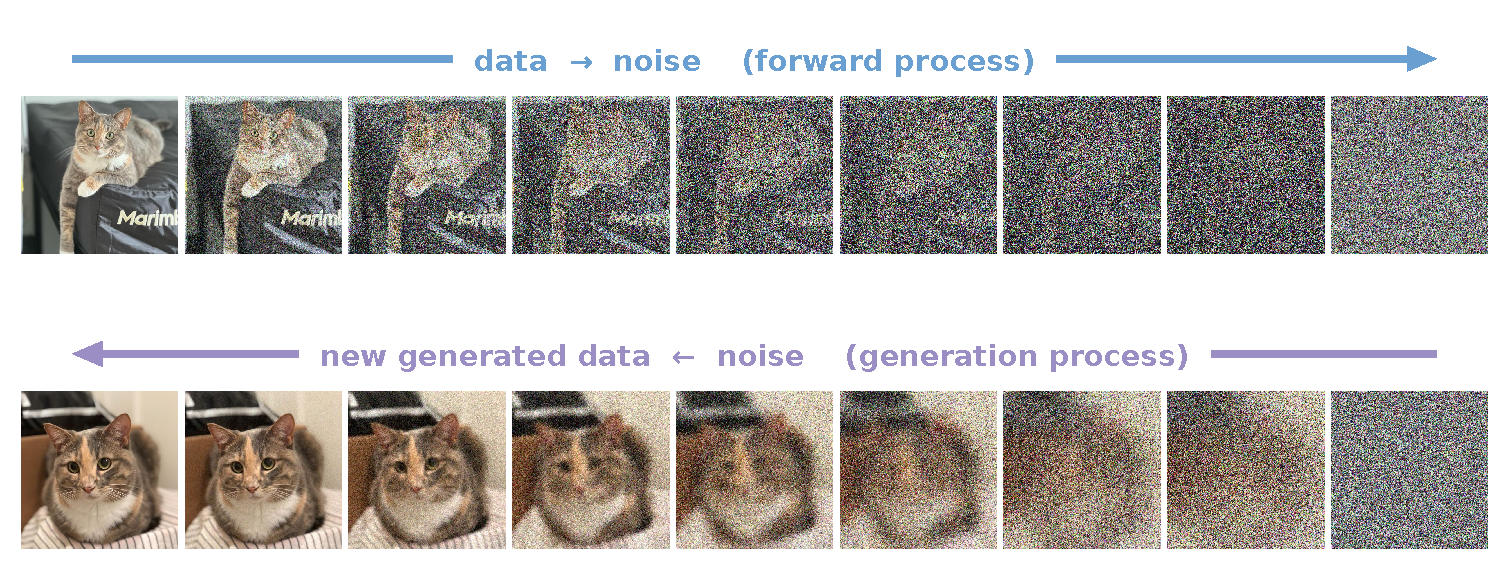
\includegraphics[width=\linewidth]{Images/PartA/diffusion_forward_vs_reverse.pdf}
    \caption{\textbfs{前向与反向扩散轨迹。}在前向过程中（上图），一个真实数据样本被噪声逐步腐蚀，经过一系列中间带噪阶段，最终变得与纯噪声难以区分。在反向过程中（下图），生成从一个全新的噪声样本开始，逐步去除噪声以产生一张新图像。反向过程并非重建训练时见过的某个特定样本，而是从全新噪声出发，逐步将其塑造成逼真的新样本。\figcredit{由作者绘制。}}
    \label{fig:ill-forward-reverse}
\end{figure}

在概述了深度生成式建模的一般目标和机制之后，我们现在转向扩散模型——一类将生成实现为从噪声到数据渐进变换的方法（见\Cref{fig:ill-forward-reverse}）。其核心思想很简单：通过不断添加噪声，可以逐步腐蚀一个数据样本，直至它与纯随机噪声无法区分。这一\emph{前向过程}将不同的数据样本映射到同一个简单的噪声空间，该空间易于采样，并作为生成的起点。在此过程中，它还创建了连接数据与噪声的一系列平滑的中间带噪阶段。在生成时，我们从这个空间中抽取一个全新的噪声样本，并通过\emph{反向（生成）过程}逐步去除噪声，最终产生一个新的数据样本。这一反向过程并不恢复某个特定的原始样本，而是从全新噪声出发，逐步将其转化为逼真的数据。我们考察三个相互关联的框架，每一个都建立在同一原理之上：一个逐步添加噪声的前向过程，以及一个由一系列逐步去噪的模型所近似的反向过程：
\begin{itemize}
    \item \textbfs{变分视角}（\Cref{ch:variational}）：源于变分自编码器（VAE）~\citep{kingma2013auto}，它通过变分目标将扩散建模为学习一个去噪过程，由此产生了去噪扩散概率模型（DDPM）~\citep{sohl2015deep,ho2020denoising}。
    \item \textbfs{分数视角}（\Cref{ch:score-based}）：植根于基于能量的模型（EBM）\\~\citep{ackley1985learning}，并发展为噪声条件分数网络（NCSN）~\citep{song2019generative}。它学习分数函数，即数据对数密度的梯度，用以指导如何逐步从样本中去除噪声。在连续时间下，\Cref{ch:score-sde} 引入了\emph{Score SDE 框架}，将这一去噪过程描述为一个随机微分方程（SDE），并将其确定性对应物描述为一个常微分方程（ODE）。这一视角将扩散建模与经典的微分方程理论联系起来，为分析和算法设计提供了清晰的数学基础。
    \item \textbfs{流视角}（\Cref{ch:flow-based}）：建立在归一化流~\citep{rezende2015variational} 之上，并由流匹配~\citep{lipman2022flow} 推广。该视角将生成建模为一个连续变换，把样本从一个简单先验传输到数据分布。这一演化由速度场通过 ODE 来支配，明确地定义了概率质量如何随时间移动。这种基于流的公式自然地超越了"先验到数据"的生成，扩展到更一般的\emph{分布到分布的转换}问题，即学习连接任意一对源分布与目标分布的流。
\end{itemize}

\begin{figure}[th!]
  \centering
  \resizebox{0.95\linewidth}{!}{%
    \begin{tikzpicture}[x=2.6cm,y=1cm,line cap=butt]
      \tikzset{>={Stealth[length=12pt,width=16pt]}}
      \def\DotR{4pt}
      \def\LabelAngle{45}
      \def\DateAboveA{32pt}
      \def\DateAboveB{32pt}
      \def\DateXShiftA{0pt}
      \def\DateXShiftB{0pt}
      \def\TextBelow{20pt}
      \def\dx{0.9}      % spacing step
      \def\XStart{0.4}  % << move EBM right by this many "x" units
      \newcommand{\nl}{\\}

      % colors
      \definecolor{PersB}{HTML}{FF7F0E} % EBM, NCSN, Score SDE
      \definecolor{PersA}{HTML}{1F77B4} % VAE, DPM, DDPM
      \definecolor{PersC}{HTML}{2CA02C} % NF, NODE, FM

      % Chronological list (even spacing by index)
      \def\Events{
        {1985/01}/{\color{PersB}{EBM}},
        {2013/12}/{\color{PersA}{VAE}},
        {2014/12}/{\color{PersC}{NF}},
        {2015/05}/{\color{PersA}{DPM}},
        {2018/06}/{\color{PersC}{NODE}},
        {2019/07}/{\color{PersB}{NCSN}},
        {2020/06}/{\color{PersA}{DDPM}},
        {2020/11}/{\color{PersB}{Score SDE}},
        {2022/10}/{\color{PersC}{FM}}
      }

      % axis
      \pgfmathsetmacro{\N}{9}
      \draw[ultra thick,-Stealth] (0,0) -- ({\XStart + (\N-1)*\dx + 0.8},0);

      % draw items
      \foreach [count=\i] \date/\desc in \Events {
        \pgfmathsetmacro{\xx}{\XStart + (\i-1)*\dx}
        \fill[black] (\xx,0) circle[radius=\DotR];

        % date above (vertical, staggered)
        \ifodd\i
          \node[above=\DateAboveA,align=center,rotate=90,inner sep=1pt,
                xshift=\DateXShiftA] at (\xx,0) {\date};
        \else
          \node[above=\DateAboveB,align=center,rotate=90,inner sep=1pt,
                xshift=\DateXShiftB] at (\xx,0) {\date};
        \fi

        % label below (45°)
        \node[below=\TextBelow,anchor=north,rotate=\LabelAngle,inner sep=1pt] at (\xx,0)
          {\shortstack[c]{\strut \desc}};
      }
    \end{tikzpicture}%
  }
  \caption{\textbfs{扩散模型各视角的时间线。}每组共享同一颜色。
  \\
\sqbullet\ 在\Cref{ch:variational} 中，{变分自编码器（VAE）}~\citep{kingma2013auto} $\to$ {扩散概率模型（DPM）}~\citep{sohl2015deep} $\to$
{DDPM}~\citep{ho2020denoising}。
 \\
\sqbullet\ 在\Cref{ch:score-based,ch:score-sde} 中，{基于能量的模型（EBM）}~\citep{ackley1985learning} $\to$ {噪声条件分数网络（NCSN）}~\citep{song2019generative} $\to$ {Score SDE}~\citep{song2020score}。  \\
\sqbullet\
在\Cref{ch:flow-based} 中，{归一化流（NF）}~\citep{rezende2015variational} $\to$ {神经 ODE（NODE）}~\citep{chen2018neural} $\to$ {流匹配（FM）}~\citep{lipman2022flow}。
\figcredit{由作者绘制。}}
  \label{fig:timeline-diffusion-perspectives-equal}
\end{figure}

尽管这些视角乍看之下各不相同，但\Cref{ch:all-equivalent} 表明它们之间存在着深刻的联系。
每一种都采用了\emph{条件化策略}，将学习目标转化为一个可处理的回归问题。
在更深层次上，它们都描述了概率分布从先验到数据的同一种时间演化。
这一演化由\emph{Fokker–Planck 方程}所支配，该方程可被视为密度的连续时间变量替换，确保了随机性与确定性公式之间的一致性。

既然扩散模型可以被视为将一个分布传输到另一个分布的方法，\Cref{ch:ot-eot} 发展了它们与经典最优传输和薛定谔桥之间的联系，后者可解释为带熵正则化的最优传输。我们回顾了静态和动态两种公式，并解释了它们与连续性方程以及 Fokker--Planck 视角的关系。对于关注实用层面的读者而言，本章是可选的；但对于希望深入研究这些联系的读者，本章提供了严格的数学背景，并指出了相关经典文献的入口。

% \ys{Some quick thoughts as I read through this part: I like how you categorize the main perspectives on diffusion into three groups, but it feels a bit odd to propose unifying them under the score SDE framework. I tend to view the score SDE framework as part of the score-based perspective. Moreover, the flow-based view emerged after the development of the score SDE framework, so it feels like an overstatement to suggest that it can be directly implied by the score SDE framework.}

%%%%%%%%%
\begin{figure}[ht!]
\begin{center}
\resizebox{\textwidth}{!}{%
\begin{tikzpicture}[
  box/.style = {draw, rounded corners, minimum width=3.6cm, minimum height=1.5cm, align=center},
  model/.style = {draw, fill=gray!20, minimum width=3.5cm, minimum height=1cm, align=center},
  arrow/.style = {ultra thick, -{Stealth[length=4mm, width=4mm]}}
  ]


   
% 2nd layer: Origin
\node[box] (vae) {Variational \\Autoencoder};
\node[box, right=1.2cm of vae] (ebm) {Energy-Based Model};
\node[box, right=1.2cm of ebm] (flow) {Normalizing Flows};

% Box around diffusion models
\node[draw, rounded corners, minimum width=13.6cm, minimum height=1.0cm, thick, above=3.5cm of ebm, label=above:{\parbox{5cm}{ \centering {Chapter}~\ref{ch:overview-dgm} 
 }}] (dgm) {Overview of Deep Generative Modeling};
  
% Top layer: Origin
\node[model, above=1.5cm of vae] (variational-based) {\large\textbfs{Variational View}};
\node[model, above=1.5cm of ebm] (score-based) {\large\textbfs{Score-Based View}};
\node[model, above=1.5cm of flow] (flow-based) {\large\textbfs{Flow-Based View}};

% Bottom layer: Diffusion Models
\node[box, below=2.2cm of vae] (ddpm) {Denoising Diffusion\\Probabilistic Model\\ (DDPM)};
\node[box, below=2.2cm of ebm] (score) {Noise Conditional\\Score Network \\(NCSN)};
\node[box, below=2.2cm of flow] (gfm) {Gaussian\\Flow Matching};

% Draw arrows
\draw[arrow] (vae.south) -- node[midway, anchor=center, yshift=3.5pt, xshift=-8pt] {\rotatebox{90}{\small {Chapter~\ref{ch:variational}}}} (ddpm.north);

\draw[arrow] (ebm.south) -- node[midway, anchor=center, yshift=3.5pt, xshift=-8pt] {\rotatebox{90}{\small {Chapter}~\ref{ch:score-based}}} (score.north);

\draw[arrow] (flow.south) -- node[midway, anchor=center, yshift=3.5pt, xshift=-8pt] {\rotatebox{90}{\small {Chapter}~\ref{ch:flow-based}}} (gfm.north);

\node[box, below=2cm of score] (scoresde) { Continuous-Time Formulation \\ (e.g., Score SDE) \\ \small {Chapter}~\ref{ch:score-sde}};

% Box around diffusion models
\node[draw, rounded corners, thick, fit={(ddpm) (score) (gfm) (scoresde)}, inner sep=0.3cm, label=below:{\parbox{5cm}{\centering\textbfs{\\ \large Unifying Principles}  \\ \vspace{0.2cm}\small {Chapter}~\ref{ch:all-equivalent} 
\begin{itemize}
    \item Conditional Strategy 
    \item Fokker-Planck Equation
\end{itemize} }}] (box) {};


\draw[ultra thick, -{Stealth[length=4mm, width=4mm]}, rounded corners=4pt] (ddpm.south) -- ++(0,-0.4) -- ([xshift=-1.0cm]scoresde.north);
\draw[ultra thick, -{Stealth[length=4mm, width=4mm]}, rounded corners=4pt] (score.south) -- ++(0,-0.4) -- (scoresde.north);
\draw[ultra thick, -{Stealth[length=4mm, width=4mm]}, rounded corners=4pt] (gfm.south) -- ++(0,-0.4) -- ([xshift=1.0cm]scoresde.north);

% Add labels
\node[align=center, left=0.5cm of box, yshift=8.3cm] {\rotatebox{90}{\textbfs{\large{Perspective}}}};
\node[align=center, left=0.5cm of box, yshift=5.5cm] {\rotatebox{90}{\textbfs{\large{Origin}}}};
\node[align=center, left=0.5cm of box] {\rotatebox{90}{\textbfs{\large{Diffusion Model}}}};
\end{tikzpicture}
 % end resizebox
    }
\end{center}
\caption{\textbfs{B 部分：扩散模型的统一与原理性视角。}此图直观地将经典生成式建模方法——变分自编码器、基于能量的模型和归一化流——与它们对应的扩散模型公式联系起来。每条纵向路径展示了一条概念脉络，最终汇聚到连续时间框架。三种视角（变分、分数和流）提供了截然不同却在数学上等价的解释。\figcredit{由作者绘制。}}
\label{fig:part-b-roadmap}
\end{figure}

%%%%%%%%%%%%%%%

%%%%%%%%%%%%%%

\paragraph{C 部分与 D 部分：控制与加速扩散采样。}

在统一了基础原理之后，我们转向利用扩散模型进行高效生成的实用层面。从扩散模型中采样对应于求解一个微分方程。然而，这一过程通常计算开销较大。C 部分和 D 部分聚焦于通过增强采样和学习型加速技术来改善生成质量、可控性和效率。



\subparagraph{C 部分：从扩散模型采样。}扩散模型的生成过程展现出独特的由粗到细的精炼：噪声被逐步去除，产生结构连贯性和细节不断增强的样本。这一特性带来了权衡。一方面，它提供了细粒度的控制；通过在学习到的、随时间变化的速度场上添加一个引导项，我们可以引导 ODE 流以反映用户意图，使采样变得可控。另一方面，所需的迭代积分使得采样相比单步生成器要缓慢。
本部分聚焦于在推理时改进生成过程，且无需重新训练。
\begin{itemize}
    \item \textbfs{引导生成}（\Cref{ch:guidance}）\textbfs{:} 诸如分类器引导和无分类器引导等技术，使得生成过程能够以用户定义的目标或属性为条件。在此基础上，我们接下来讨论如何使用偏好数据集进一步将扩散模型与这些偏好相对齐。
    \item \textbfs{用数值求解器实现快速生成}（\Cref{ch:solvers}）\textbfs{:} 使用先进的数值求解器可以在更少的步数内近似反向过程，从而显著加速采样，在降低开销的同时保持质量。
\end{itemize}
\subparagraph{D 部分：学习快速的生成式模型。}除了改进现有的采样算法，我们还研究如何直接学习能够近似扩散过程的快速生成器。
\begin{itemize}
    \item \textbfs{基于蒸馏的方法}（\Cref{ch:distillation}）：该方法聚焦于训练一个学生模型来模仿一个预训练的、缓慢的扩散模型（教师模型）的行为。其目标不是缩小教师模型的规模，而是以远少得多的积分步数（通常只有几步甚至一步）重现其采样轨迹或输出分布。
    \item \textbfs{从零开始学习}（\Cref{ch:fast-scratch}）\textbfs{:} 既然扩散模型中的采样可以被视为求解一个 ODE，该方法便从零开始直接学习该解的映射（即流映射），而无需依赖教师模型。学习到的映射可以直接将噪声变为数据，或更一般地在求解轨迹上执行任意时刻到任意时刻的跳跃。
\end{itemize}


% \ys{Should we call it ``distillation-based methods''? Not sure distillation is one type of post-training. That said, we may indeed want to discuss post-training techniques for diffusion models in nearby sections on ``steering generation''. }

\paragraph{尾声：超越连续状态空间上的扩散。}
我们在\Cref{ch:epilogue} 中明确指出贯穿全书的核心原理。从本质上讲，扩散建模并不绑定于某一种特定的噪声类型、模型类别，甚至不绑定于连续状态空间。它所研究的，是概率质量在一个预先规定的时间相关的前向腐蚀过程下如何演化，以及这种演化如何被反转、被近似、或被用于生成。在连续设定下，这一原理通过变量替换公式、连续性方程和 Fokker--Planck 方程体现。在离散设定下，相同结构性作用由转移核、连续时间马尔可夫链和主方程承担。

最后这一章还表明，本书贯穿始终所发展的三种视角——即变分、分数和流视角——超越了连续数据建模。即便对于文本、蛋白质序列以及其他基于词元的对象等离散数据，人们仍然可以通过变分目标、类似分数的比率或反向速率刻画，以及类似流的传输视角来 formulate 反向建模。数学对象改变了，但底层原理并未改变。如此一来，尾声既是全书在概念上的总结，也指向了生成式建模更广阔图景的展望。


\paragraph{附录。}
为确保这段旅程对所有读者都易于理解，附录提供了基础概念的背景知识。\Cref{app:de} 提供了一份关于微分方程的速成课程，微分方程已成为扩散模型的语言。

尽管扩散模型视角和起源各异，其背后的核心洞见在于\emph{变量替换公式}。这一基础自然延伸到更深层的概念，如\emph{Fokker--Planck 方程}和\emph{连续性方程}，它们描述了概率密度如何由函数（离散时间）或微分方程（连续时间）定义的映射所变换和演化。
\Cref{app:continuity} 提供了一份平易近人的介绍，将这些基础思想桥接到更高级的概念。
在\Cref{app:Ito} 中，我们呈现了扩散模型背后两个强大却常被忽视的工具：\emph{Itô 公式}和\emph{Girsanov 定理}，它们为 Fokker--Planck 方程和反向采样过程提供了严格的支持。
最后，\Cref{app:proof} 汇集了正文章节中部分命题和定理的证明。


% \paragraph{What this Book Covers and What Does Not?}

% Overall, from the top-down viewpoint this book covers from the core principle of ``constructing the dynamics that transporting in continuous time from the simple prior distribution to the data distribution while making the distribution at each time snapshot matches with the distributions of pre-scribed process from data-to-noise''. Starting from this diffusion-modeling principle, we discuss the stochastic/deterministic flow to realize the sampling transportation, and establish the controllable and faster way of achieving this transportation.  We do not cover the detailed practical implementations, engineering know-hows, models or architectureal selections, datasets benchmarking, or domain-specific applications. 



\paragraph{本书涵盖的内容与不涵盖的内容。}
我们追求经久耐用。从自顶向下的视角来看，本书从一个单一原理出发：构造连续时间的动力学，将一个简单先验传输到数据分布，同时确保每一时刻的边缘分布与一个预先规定的前向过程（从数据到噪声）所诱导的边缘分布相匹配。从这一原理出发，我们发展了实现采样的随机流和确定性流，展示了如何引导轨迹（引导），并解释了如何加速它（数值求解器）。然后，我们研究受扩散启发的快速生成器，包括蒸馏方法和流映射模型。借助这些工具，读者可以将新论文纳入一个共同模板，理解方法为何有效，并设计出改进的模型。

我们并不试图对扩散模型文献进行穷尽式的综述，也不罗列架构、训练实践、超参数，不对各方法的经验结果进行比较，不涵盖数据集和排行榜，不描述特定领域或模态的应用，不讨论系统级部署，不提供大规模训练的配方，也不讨论硬件工程。这些主题演变迅速，更适合由专题综述、开放仓库和实现指南来涵盖。







% \begin{figure}[th!]
% \caption{\textbfs{Part C. Sampling with Diffusion Models.} \Cref{ch:score-sde} shows that diffusion model sampling is equivalent to solving an ODE. From this view, the \textit{left branch} interprets guided generation as steering the velocity field with auxiliary signals. As this process involves solving differential equations, it is inherently slow. To mitigate this, the \textit{middle branch} employs classical numerical solvers to accelerate sampling by efficiently estimating the integral using a pre-trained model $\rvv$. \\
% \textbfs{Part D. Learning a Fast Diffusion-Based Generator.} The \textit{right branch} takes a different route: directly learning to approximate the ODE solution or its distribution at $t=0$, either using a pre-trained model or training from scratch. The latter yields a standalone generator that avoids costly sampling.
% }
% \begin{center}
% \resizebox{\textwidth}{!}{% 
% \centering
% \begin{tikzpicture}[
%     box/.style={rectangle, draw, thick, minimum width=3cm, minimum height=2cm, align=center},
%     topbox/.style={rectangle, draw, thick, minimum width=12cm, minimum height=1.5cm, align=center},
%     arrow/.style={->, thick},
%     roundbox/.style={rectangle, draw, thick, rounded corners=10pt, minimum width=4cm, minimum height=3cm, align=center}
% ]

% % Top box
% \node[topbox, label=above:{\parbox{5cm}{\centering  {Chapter}~\ref{ch:score-sde}}}] (top) at (0,4) {\\
% \textbfs{Generation with Diffusion Model $\mathbf{v}(\rvx, t)$} \\[0.3cm]
% $\Longleftrightarrow$ Solve ODE backward from $t = T$ to $0$ with $\mathbf{x}(T) \sim p_{\mathrm{prior}}$: \\[0.2cm]
% $\displaystyle\frac{\diff\mathbf{x}(t)}{\diff t} = \mathbf{v}(\mathbf{x}(t), t)$ \\[0.3cm]
% $\displaystyle\Longleftrightarrow \mathbf{x}(0) = \mathbf{x}(T) + \int_0^T \mathbf{v}(\mathbf{x}(t), t)\diff t$
% };

% % Three bottom boxes
% \node[roundbox, label=below:{\parbox{5cm}{\centering  {Chapter}~\ref{ch:guidance} 
%  }}] (left) at (-6,-2) {
% \\ \large\textbfs{Steering Generation} \\[0.4cm]
% \parbox{5cm}{
% \begin{align*}
%     \displaystyle\mathbf{x}(0) &= \mathbf{x}(T) + \int_0^T [\mathbf{v}(\mathbf{x}(t), t) \\ 
%     &\qquad \textcolor{darkgray}{+ \textbf{Guidance}}] \diff t
% \end{align*}}
% };

% \node[roundbox, label=below:{\parbox{5cm}{\centering {Chapter}~\ref{ch:solvers} 
%  }}] (center) at (0,-2) {
% \\ \large\textbfs{Fast Generation} \\
% \large\textbfs{with Numerical Solvers} \\[-0.6cm]
% $\displaystyle\mathbf{x}(0) = \mathbf{x}(T) + \eqnmarkbox[Plum]{velocity}{\int_0^T \mathbf{v}(\mathbf{x}(t), t)\diff t}$ \\[-0.8cm]
% Estimating the integral
% };

% \node[roundbox, label=below:{\parbox{5cm}{\centering  {Chapter}~\ref{ch:distillation} and {Chapter}~\ref{ch:fast-scratch} 
%  }}] (right) at (6,-2) {
% \\ \large\textbfs{Learning a Fast} \\
% \large\textbfs{Diffusion-Based Generator} \\[-0.6cm]
% $\displaystyle\mathbf{x}(0) = \eqnmarkbox[Pink]{target}{\mathbf{x}(T) + \int_0^T \mathbf{v}(\mathbf{x}(t), t)\diff t}$ \\[-0.8cm]
% Learning the Integral
% };

% % Arrows
% \draw[ultra thick, -{Stealth[length=4mm, width=4mm]}, rounded corners=4pt] (top.south) -- ++(-6,-1) -- (left.north);
% \draw[ultra thick, -{Stealth[length=4mm, width=4mm]}, rounded corners=4pt] (top.south) -- (center.north);
% \draw[ultra thick, -{Stealth[length=4mm, width=4mm]}, rounded corners=4pt] (top.south) -- ++(6,-1) -- (right.north);

% \end{tikzpicture}
% }
% \end{center}
% \label{fig:part-c-d-roadmap}
% \end{figure}

% \se{i don't think this figure will make sense to readers that don't already know diffusion}

% \se{btw, i think it's integral not integration}
%%%%%%%%%%%%%%%




\chapter*{符号说明}
\markboth{\sffamily\slshape 符号说明}{\sffamily\slshape 符号说明}

%% Consistent section title command for this page
\newcommand{\notationsection}[1]{%
  \vspace{1.2em}%
  \noindent{\textbfs{#1}}%
  \vspace{0.4em}%
  \par\nobreak
}

%% Shared table setup
\newcommand{\notationtable}[1]{%
  \bgroup
  \def\arraystretch{1.25}%
  \noindent\begin{tabular}{@{}p{0.3\linewidth}@{\hspace{1.5em}}p{0.64\linewidth}@{}}
  #1
  \end{tabular}
  \egroup
}

%%% ---------------------------------------------------------------
\notationsection{数与数组}
\notationtable{
$a$                                       & 标量。\\
$\rva$                                    & 列向量（例如 $\rva\in\mathbb{R}^D$）。\\
$\rmA$                                    & 矩阵（例如 $\rmA\in\mathbb{R}^{m\times n}$）。\\
$\rmA^\top$                               & $\rmA$ 的转置。\\
$\Tr(\rmA)$                               & $\rmA$ 的迹。\\
$\rmI_D$                                  & $D\times D$ 的单位矩阵。\\
$\rmI$                                    & 单位矩阵；维数由上下文确定。\\
$\mathrm{diag}(\rva)$                     & 以 $\rva$ 为对角元的对角矩阵。\\
$\bm{\phi},\,\bm{\theta}$                & 可学习的神经网络参数。\\
$\bm{\phi}^{\times},\,\bm{\theta}^{\times}$ & 训练后的参数（在推理阶段固定）。\\
$\bm{\phi}^{*},\,\bm{\theta}^{*}$        & 优化问题的最优参数。\\
}

%%% ---------------------------------------------------------------
\notationsection{微积分}
\notationtable{
$\dfrac{\partial \rvy}{\partial \rvx}$
    & $\rvy$ 对 $\rvx$ 的偏导数（逐分量）。\\[6pt]
$\dfrac{\diff \rvy}{\diff \rvx}$ \text{或} $\mathrm{D}\rvy(\rvx)$
    & $\rvy$ 对 $\rvx$ 的（Fréchet）全导数。\\[6pt]
$\nabla_\rvx y$
    & 标量函数 $y:\mathbb{R}^D \to\mathbb{R}$ 的梯度；$\mathbb{R}^D$ 中的列向量。\\
$\dfrac{\partial \rmF}{\partial \rvx}$ \text{或} $\nabla_\rvx \rmF$
    & $\rmF:\mathbb{R}^n \to\mathbb{R}^m$ 的雅可比矩阵；形状为 $m\times n$。\\[6pt]
$\nabla\cdot\rvy$
    & 向量场 $\rvy:\mathbb{R}^D \to\mathbb{R}^D$ 的散度；一个标量。\\
$\nabla^2_\rvx f(\rvx)$ \text{或} $\rmH(f)(\rvx)$
    & $f:\mathbb{R}^D \to\mathbb{R}$ 的海森矩阵；形状为 $D\times D$。\\
$\displaystyle\int f(\rvx)\diff\rvx$
    & $f$ 在 $\rvx$ 的定义域上的积分。\\
}

%%% ---------------------------------------------------------------
\notationsection{概率论与信息论}
\notationtable{
$p(\rvx)$                   & 连续向量 $\rvx$ 上的密度/分布。\\
$\Pr(\rvx = \rva)$，或非正式地写作 $\Pr(\rvx)$
    & 离散情形下的点概率。\\
$\Pr(\rvx = \rva |\rvy = \rvb)$，或非正式地写作 $\Pr(\rvx |\rvy)$
    & 离散情形下的条件点概率。\\
$p_{\mathrm{data}}$        & 数据分布。\\
$p_{\mathrm{prior}}$       & 先验分布（例如标准正态分布）。\\
$p_{\mathrm{src}}$         & 源分布。\\
$p_{\mathrm{tgt}}$         & 目标分布。\\
$\rva \sim p$              & 随机向量 $\rva$ 服从分布 $p$。\\
$\E_{\rvx\sim p}\big[\rvf(\rvx)\big]$
    & $\rvf(\rvx)$ 在 $p(\rvx)$ 下的期望。\\[3pt]
\parbox[t]{0.22\linewidth}{\raggedright
  $\E\big[\rvf(\rvx)\,|\,\rvz\big]$，\\[2pt]
  或 $\E_{\rvx\sim p(\cdot|\rvz)}\big[\rvf(\rvx)\big]$}
    & 给定 $\rvz$ 时 $\rvf(\rvx)$ 的条件期望，其中 $\rvx$ 服从 $p(\cdot|\rvz)$。\\[3pt]
$\Var\big(\rvf(\rvx)\big)$
    & 在 $p(\rvx)$ 下的方差。\\
$\Cov\big(\rvf(\rvx),\rvg(\rvx)\big)$
    & 在 $p(\rvx)$ 下的协方差。\\
$\mathcal{D}_{\mathrm{KL}}\left(p\,\Vert\, q\right)$
    & 从 $q$ 到 $p$ 的 Kullback--Leibler 散度。\\
$\bm{\epsilon}\sim\mathcal{N}(\bm{0},\rmI)$
    & 标准正态分布的样本。\\
$\mathcal{N}(\rvx;\vmu,\mSigma)$
    & $\rvx$ 上的高斯分布，均值为 $\vmu$，协方差为 $\mSigma$。\\
}

%%% ---------------------------------------------------------------
\vspace{1.2em}

\paragraph{记号约定。}
本书通篇使用若干约定，在此一并说明。

\subparagraph{I. 随机变量及其取值。}
我们对随机向量及其取值（实现值）使用相同的符号。
这一约定在深度学习和生成建模中很常见，可以使记号更紧凑。其具体含义由上下文确定。

对于密度函数，$p(\rvx)$ 表示分布的函数形式，而不是在某个具体样本处的取值。当
需要在某个具体点处求值时，我们会明确说明。
条件密度由上下文来理解：在 $p(\rvx|\rvy)$ 中，固定
$\rvy$ 得到关于 $\rvx$ 的密度函数，而固定 $\rvx$ 则得到关于
$\rvy$ 的函数。

\subparagraph{II. 条件期望。}
表达式 $\E[\rvf(\rvx)|\rvz]$ 表示关于 $\rvz$ 的函数，
给出在给定 $\rvz$ 的条件下 $\rvf(\rvx)$ 的期望值。
当以某个具体的取值为条件时，我们记作
$\E[\rvf(\rvx)|\rmZ = \rvz]$。等价地，这可以表示为
关于条件分布的积分：
\[
\E_{\rvx \sim p(\cdot|\rvz)}[\rvf(\rvx)]
= \int \rvf(\rvx)\, p(\rvx|\rvz)\, \diff\rvx.
\]
这种区分可以澄清 $\rvz$ 是被当作定义函数 $\rvz \mapsto \E[\rvf(\rvx)|\rvz]$ 的变量，
还是被当作对该函数求值的固定点。

\subparagraph{III. 隐含的时间下标。}
由于本书中的许多对象都以时间作为下标，把每个
时间变量都显式写出会使公式显得繁重。当相关的时间
下标能从上下文中清楚看出时，我们将其省略。例如，
\[
\E[\rvx_s | \rvx_t]
\quad\text{简写为}\quad
\E[\rvx_s | \rvx_t,\, s,\, t],
\]
即在时间 $t$ 给定 $\rvx_t$ 的条件下，$\rvx_s$ 在时间 $s$ 处的
平均，其中 $s$ 和 $t$ 的含义由上下文确定。
类似地，$p(\rvx_s | \rvx_t)$ 表示给定 $\rvx_t$ 时 $\rvx_s$ 的条件分布，
两个时间下标都隐含其中。

\subparagraph{IV. 高斯扰动与依分布相等。}
对于固定的下标 $t$，我们经常使用如下高斯扰动核：
\[
p_t(\rvx_t|\rvx_0)
= \mathcal{N}\big(\rvx_t;\, \alpha_t \rvx_0,\, \sigma_t^2 \rmI\big),
\]
其中 $\rvx_0 \sim p_{\mathrm{data}}$，$\alpha_t$ 和 $\sigma_t$ 是
确定性的标量。我们等价地将其写成\emph{依分布成立}的等式
\[
\rvx_t \stackrel{d}{=} \alpha_t \rvx_0 + \sigma_t \beps,
\qquad
\beps \sim \mathcal{N}(\bm{0}, \rmI),
\]
其中 $\beps$ 与 $\rvx_0$ 独立。符号
``$\stackrel{d}{=}$'' 表示两边具有相同的概率律，因此
\[
    \E[\phi(\rvx_t)] = \E[\phi(\alpha_t \rvx_0 + \sigma_t \beps)]
\]
对于任意测试函数 $\phi$ 均成立。为简便起见，我们将直接
写作 $\rvx_t = \alpha_t \rvx_0 + \sigma_t \beps$，根据上下文理解为
依分布相等或一次样本实现；本书通篇采用这一简写。

\part{深度生成式建模导论}
\chapter{深度生成式建模}\label{ch:overview-dgm}

\epigraph{
    \textit{我所不能创造的，我就不能理解。}}{Richard P. Feynman}

% \ys{This might be a good place to quote Richard Feynmann on ``What I cannot create, I do not understand.''}

% \jcc{need to rewrite the following: 
% At the heart of deep generative modeling (DGMs) is a compelling goal: teaching machines to create. Picture a system that studies thousands of images, musical pieces, or artworks—and then conjures something entirely new, yet strikingly faithful to the style and structure of its inspirations. This is more than copying; it is a learned capacity to generate original content grounded in the patterns of real-world data.}

% Deep generative models (DGMs) aim to approximate the complex and high dimensional probability distributions underlying real world data. Through unsupervised learning, they acquire the ability to synthesize novel artifacts such as images, text, video, or audio that are statistically consistent with the learned distribution.
% \se{this paragraph could be made more precise and clear}

深度生成模型（DGM）是学习高维数据（如图像、文本、音频）上概率分布的神经网络，从而能够生成与数据集相似的新样本。我们用 $p_{\bphi}$ 表示模型分布，用 $p_{\mathrm{data}}$ 表示数据分布。给定一个有限的数据集，我们通过最小化衡量 $p_{\bphi}$ 与 $p_{\mathrm{data}}$ 之间差距的损失来拟合 $\bphi$。训练完成后，生成即运行模型的采样过程以抽取 $\rvx \sim p_{\bphi}$（密度 $p_{\bphi}(\rvx)$ 能否直接计算取决于模型类别）。模型质量由生成的样本及其汇总统计量与 $p_{\mathrm{data}}$ 的匹配程度，连同任务特定或感知度量来评判。


本章构建了这些思想背后的数学与概念基础。我们在 \Cref{sec:formulation-dgm} 中形式化该问题，在 \Cref{sec:examples-dgm} 中介绍代表性的模型类别，并在 \Cref{sec:taxonomy} 中总结实用的分类体系。








% \ys{This type of motivating language is crucial to the success of the monograph, but it currently lacks the depth and force that a compelling vision should convey. I'd like to try rewriting all such paragraphs once we've addressed all the other issues.}
% \jcc{I rewrote it as the above brown part.}


% To understand how this creative synthesis becomes feasible, this chapter establishes the mathematical and conceptual foundations of modern generative models.

% We begin by formalizing the core problem in \Cref{sec:formulation-dgm}, introducing the key mathematical tools and notation that drive this field. While a diverse array of DGMs exists, as overviewed in \Cref{sec:examples-dgm}, our focus will narrow to three prominent classes of DGMs that are closely connected to diffusion models. These are: Variational Autoencoders (VAEs), which we discuss in \Cref{sec:vae}; Energy-Based Models (EBMs), introduced in \Cref{sec:ebm}; and Normalizing Flows (NFs), explored in \Cref{sec:flow-based-method}.  Through this exploration, readers will gain a comprehensive understanding of the principled foundations that underpin modern diffusion-based generative modeling, as developed in subsequent chapters.


\newpage
\section{什么是深度生成式建模？}\label{sec:formulation-dgm}

% \se{i feel a more algorithmic description describing the inputs (data) and the output (trained network) is the right level of abstraction to start}



DGM 以从未知且复杂的分布 $p_{\mathrm{data}}$ 中抽取的大量真实世界样本
（如图像、文本）作为输入，
输出一个参数化近似分布 $p_{\bphi}$ 的、已训练好的神经网络。其目标有两方面：
\begin{enumerate}
\item \textbfs{逼真生成：}生成与真实数据无法区分的、新颖逼真的样本。
\item \textbfs{可控生成：}实现对生成过程的细粒度、可解释的控制。
\end{enumerate}



% \ys{The words ``mimicry'' and ``mastery'' are unnecessarily obscure in this context.} \jcc{revised!}

% The capabilities of DGMs extend far beyond data synthesis. They have emerged as foundational tools across a wide range of domains: from restoring corrupted data and intelligently filling in missing information (inpainting) to simulating complex phenomena and driving new forms of creative content generation. \se{a bit odd to have this text here, isn't it contrallable generation?}

本节介绍 DGM 背后的基本概念与动机，为后续详细探讨其数学框架与实际应用做准备。


\subsection{数学设定}\label{subsec:intro-math-setup}
我们假设可以获得从潜在的复杂数据分布 $ p_{\mathrm{data}}(\mathbf{x}) $ 中独立同分布（i.i.d.）抽取的一组有限样本\footnote{这是机器学习中的常见假设。为简便起见，我们用符号 $ p $ 同时表示概率分布或其概率密度/质量函数，视上下文而定。}。


\paragraph{DGM 的目标。}

DGM 的首要目标是从有限数据集中学习一个可处理的概率分布。这些数据点是假设从未知且复杂的真实分布 $p_{\mathrm{data}}(\rvx)$ 中采样得到的观测值。由于 $p_{\mathrm{data}}(\rvx)$ 的形式未知，我们无法直接从中抽取新样本。因此，核心挑战在于构建一个能够充分近似该分布的模型，以实现新逼真样本的生成。

为此，DGM 使用深度神经网络来参数化模型分布 $p_{\bm{\phi}}(\rvx)$，其中 $\bm{\phi}$ 表示网络的可训练参数。训练目标是找到最优参数 $\bm{\phi}^\ast$，使模型分布 $p_{\bm{\phi}}(\rvx)$ 与真实数据分布 $p_{\mathrm{data}}(\rvx)$ 之间的散度最小。从概念上讲，
\[
p_{{\bm{\phi}}^\ast}(\rvx) \approx p_{\mathrm{data}}(\rvx).
\]




% The primary objective of deep generative modeling (DGM) is to learn \se{learn what?} from a finite dataset sampled from an unknown true distribution $p_{\mathrm{data}}(\mathbf{x})$, and to generate new samples that closely resemble this data. Since the explicit form of $p_{\mathrm{data}}(\mathbf{x})$ is unknown, the core challenge lies in approximating and efficiently sampling from this complex distribution \se{confusing, we never sample from pdata, only pmodel} to enable realistic and data-consistent generation based on limited observations.


% To this end, we use a deep neural network to construct a parametrized model density $p_{\bm{\phi}}(\rvx)$, where ${\bm{\phi}} \in \Phi$ denotes the model parameters \se{model and network terminology creates unnecessary ambiguity} and $\Phi$ represents the set of all possible parameter values. The objective is to find the optimal parameters ${\bm{\phi}}^\ast \in \Phi$ such that  
% \[
% p_{{\bm{\phi}}^\ast}(\rvx) \approx p_{\mathrm{data}}(\rvx).
% \]
% \se{i would rephrase slightly to avoid the potential confusion that networks have finite capacity so the above is not possible}

当统计模型 $p_{{\bm{\phi}}^\ast}(\rvx)$ 充分逼近数据分布 $p_{\mathrm{data}}(\rvx)$ 时，它可以作为生成新样本和评估概率值的代理。这一模型 $p_{\bm{\phi}}(\rvx)$ 通常被称为\emph{生成模型}。


\paragraph{DGM 的能力。}
一旦有了数据分布的代理 $p_{\bm{\phi}}(\rvx)$，我们就可以使用诸如从 $p_{\bm{\phi}}(\rvx)$ 中进行蒙特卡洛采样等采样方法，生成任意数量的新数据点。此外，对于任意给定样本 $\rvx'$，我们可以评估模型密度 $p_{\bm{\phi}}(\rvx')$，这通常被非正式地称为模型赋予 $\rvx'$ 的“似然”\footnote{严格来说，对于连续数据，$p_{\bm{\phi}}(\rvx')$ 是在 $\rvx'$ 处求值的密度，而非观测到该精确样本的概率。我们遵循机器学习领域的惯常简写，将该量称为样本的“似然”。}。

\begin{figure}
\vspace{-0.5cm}
    \centering
    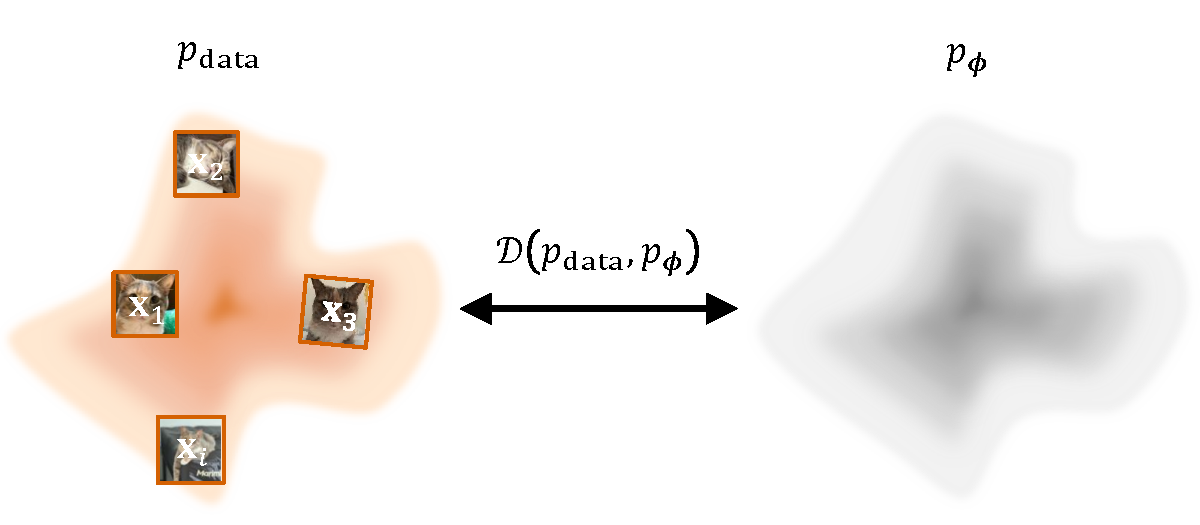
\includegraphics[width=0.9\linewidth]{Images/PartB/dgm-learning.pdf}
    \vspace{-0.2cm}
    \caption{\textbfs{DGM 目标示意图。}训练 DGM 本质上是最小化模型分布 $p_{\bm{\phi}}$ 与未知数据分布 $p_{\mathrm{data}}$ 之间的差异。由于 $p_{\mathrm{data}}$ 无法直接访问，这一差异必须利用从中抽取的有限独立同分布（i.i.d.）样本 $\rvx_i$ 来高效估计。\figcredit{由作者绘制。}}
    \label{fig:dgm-training}
\end{figure}

% \paragraph{Training of DGM.}
% To train the model, we define a discrepancy measure $\mathcal{D}(\cdot, \cdot)$ that quantifies the difference between the data distribution $p_{\mathrm{data}}$ and the model distribution $p_{\bm{\phi}}$. Since the true data distribution is unknown, this discrepancy must be estimated efficiently using a finite set of independent and identically distributed (i.i.d.) samples drawn from $p_{\mathrm{data}}$. The optimal parameter $\bm{\phi}^\ast$ is then obtained by solving the following optimization problem based on this empirical estimate:
% \begin{align}\label{eq:dgm-optimization}
%     \bm{\phi}^\ast = \arg\min_{\bm{\phi} \in \Phi} \mathcal{D}(p_{\mathrm{data}}, p_{\bm{\phi}}).
% \end{align}
% If the parameter space $\Phi$ is sufficiently large and the model family $\{p_{\bm{\phi}}\}_{\bm{\phi} \in \Phi}$ is expressive enough, then $p_{\bm{\phi}^\ast}(\mathbf{x})$ can closely approximate $p_{\mathrm{data}}(\mathbf{x})$.


% \ys{One missing factor is there must exist an efficient way to estimate this discrepancy measure using iid samples from the data distribution.}

% There are various choices for the discrepancy measure $\mathcal{D}$~\citep{cover1999elements}, including the Wasserstein distance, total variation distance, Jensen–Shannon divergence, Fisher divergence (spoiler: notably related to diffusion models), and the Kullback–Leibler (KL) divergence. Each induces a different training objective, with distinct trade-offs in sensitivity, smoothness, and optimization dynamics. Among them, the KL divergence is especially popular due to its close connection to maximum likelihood estimation, as discussed next.
% \se{instead of throwing all this jargon at the reader, i would start with an example (KL) and then tell them there are other options}

% \subparagraph{Kullback-Leibler Divergence.}
% \jc{
% A widely used choice for $\mathcal{D}$ is the Kullback–Leibler (KL) divergence, denoted by $\mathcal{D}_{\mathrm{KL}}(\cdot \| \cdot)$, which measures the discrepancy between the data distribution $p_{\mathrm{data}}$ and the model distribution $p_{\bm{\phi}}$. It is defined as
% \begin{align*}
%     \mathcal{D}_{\mathrm{KL}}(p_{\mathrm{data}} \| p_{\bm{\phi}}) 
%     &:= \int p_{\mathrm{data}}(\mathbf{x}) \log \frac{p_{\mathrm{data}}(\mathbf{x})}{p_{\bm{\phi}}(\mathbf{x})} \, \diff \mathbf{x} \\
%     &= \mathbb{E}_{p_{\mathrm{data}}} \left[ \log \frac{p_{\mathrm{data}}(\mathbf{x})}{p_{\bm{\phi}}(\mathbf{x})} \right],
% \end{align*}
% where the integral is a Lebesgue integral\footnote{Throuout the monograph, if without stating, the integration of deterministic mappings is understood as Lebesgue sense.}, which reduces to a summation when the distributions are defined over discrete spaces.

% The KL divergence is asymmetric, i.e., 
% \[
% \mathcal{D}_{\mathrm{KL}}(p_{\mathrm{data}} \| p_{\bm{\phi}}) \neq \mathcal{D}_{\mathrm{KL}}(p_{\bm{\phi}} \| p_{\mathrm{data}}).
% \]Importantly, minimizing $\mathcal{D}_{\mathrm{KL}}(p_{\mathrm{data}} \| p_{\bm{\phi}})$ encourages \emph{mode covering}: the model is penalized heavily if it assigns low probability to regions where the data density is high. This pushes the model to cover all modes of the data distribution, avoiding mode collapse.
% }
% \se{add an extra sentence actually showing it using the formula, e.g. if pmodel is zero when pdata is not}

% \ys{It may be useful to note somewhere that the integrals below refer to Lebesgue integrals, which reduce to summations when defined over counting measures.}

% \ys{No need to expand so much on the following list. Just mention it has the ``mode covering'' property, and explain what it means and why in a few sentences (ChatGPT can do this).} \jcc{Revised!}

% \se{important to note somewhere that pdata can't be evaluated, which is a good motivation for the MLE stuff below}

% Crucially, it is equivalent to \emph{Maximum Likelihood Estimation} (MLE), as detailed below.
% \subparagraph{Maximum Likelihood Training.}
% From the definition of $\mathcal{D}_{\mathrm{KL}}$, we derive:
% \begin{align*}
%     \mathcal{D}_{\mathrm{KL}}(p_{\mathrm{data}} \| p_{\bm{\phi}}) 
%     &= \displaystyle\int  \log \frac{p_{\mathrm{data}}(\mathbf{x})}{p_{\bm{\phi}}(\mathbf{x})} p_{\mathrm{data}}(\mathbf{x}) \diff \rvx \\
%     &= -\mathbb{E}_{\rvx \sim p_{\mathrm{data}}} \left[ \log p_{\bm{\phi}}(\mathbf{x}) \right] + C,
% \end{align*}
% where $C := \mathbb{E}_{\rvx \sim p_{\mathrm{data}}} \left[\log p_{\mathrm{data}}(\mathbf{x})\right]$ is constant with respect to $\bm{\phi}$. Hence, minimizing KL divergence is equivalent to maximizing the log-likelihood: 
% % \ys{``Message'' feels weird in this context. Maybe better to call it ``remark'', or ``observation''?}
% \msg{Observation}{Minimizing KL $\Leftrightarrow$ Maximum Likelihood Estimation}{
% \begin{align}\label{eq:MLE}
%     \min_{\bm{\phi}} \mathcal{D}_{\mathrm{KL}}(p_{\mathrm{data}} \| p_{\bm{\phi}}) \Longleftrightarrow \max_{\bm{\phi}}\mathbb{E}_{\rvx\sim p_{\mathrm{data}}}\left[\log p_{\bm{\phi}}(\rvx)\right].
% \end{align}
% }
% MLE is a classical method for learning probabilistic models by finding parameters $\bm{\phi}$ that maximize the likelihood of the observed data, rather than explicitly reconstructing the data points. \se{maybe move after you introduce the empirical (not population) version, otherwise there is no observation/data}

% To implement MLE in practice, we often minimize the KL divergence between the data and model distributions, approximated using a finite set of training samples  $\{\mathbf{x}^{(i)}\}_{i=1}^N$:
% \begin{align*}
%     \mathcal{D}_{\mathrm{KL}}(p_{\mathrm{data}} \| p_{\bm{\phi}}) 
%     &\approx  -\frac{1}{N} \sum_{i=1}^N \log p_{\bm{\phi}}(\mathbf{x}^{(i)}) + C,
% \end{align*}
% with $C = \frac{1}{N} \sum_{i=1}^N \log p_{\mathrm{data}}(\mathbf{x}^{(i)})$.
% \se{this is strange and potentially confusing, i would avoid the C estimate part since that is not something we can do "in practice"}


% \jc{While the model could theoretically assign arbitrarily high density to training points (a countable set with measure zero), in practice, neural networks avoid forming delta distributions due to their continuous and smooth architectures, finite capacity, and regularization (e.g., weight decay, dropout), which prevent overfitting.} \ys{I think you're confusing density functions with mass functions here. For continuous distributions, the optimal model distribution is indeed a delta distribution. The model's density function can take arbitrarily high values at data points, since these are countable. The integral of a probability density function is unaffected by its values on a countable set. The fact that our model distributions do not collapse to delta distributions cannot be attributed to the normalization constraint.} \jcc{Revised!}
% \se{not sure why overfitting/regularization is relevant here; it's not particularly specific to the loss used to train generative models}


\paragraph{DGM 的训练。}
我们通过最小化差异 $\mathcal{D}(p_{\mathrm{data}},p_{\bm{\phi}})$ 来学习模型族 $\{p_{\bm{\phi}}\}$ 的参数 $\bm{\phi}$：
\begin{align}\label{eq:dgm-optimization}
  \bm{\phi}^\ast \in \arg\min_{\bm{\phi}}\; \mathcal{D}(p_{\mathrm{data}},p_{\bm{\phi}}).
\end{align}
由于 $p_{\mathrm{data}}$ 未知，$\mathcal{D}$ 的实际选择必须能够基于来自 $ p_{\mathrm{data}} $ 的独立同分布样本进行高效估计。
在容量充足时，$p_{\bm{\phi}^\ast}$ 可以紧密逼近 $p_{\mathrm{data}}$。

\subparagraph{前向 KL 与最大似然估计（MLE）。}
一个标准选择是（前向）Kullback--Leibler 散度\footnote{所有积分均按勒贝格意义理解，在计数测度下退化为求和。}
\begin{align*}
\mathcal{D}_{\mathrm{KL}} \big(p_{\mathrm{data}}\|p_{\bm{\phi}}\big)
  := &\int p_{\mathrm{data}}(\rvx)\,\log\frac{p_{\mathrm{data}}(\rvx)}{p_{\bm{\phi}}(\rvx)}\,\diff \rvx \\
  = &\mathbb{E}_{\rvx\sim p_{\mathrm{data}}} \big[\log p_{\mathrm{data}}(\rvx)-\log p_{\bm{\phi}}(\rvx)\big].
\end{align*}
它是非对称的，即，
\[
\mathcal{D}_{\mathrm{KL}}(p_{\mathrm{data}} \| p_{\bm{\phi}}) \neq \mathcal{D}_{\mathrm{KL}}(p_{\bm{\phi}} \| p_{\mathrm{data}}).
\]重要的是，最小化 $\mathcal{D}_{\mathrm{KL}}(p_{\mathrm{data}} \| p_{\bm{\phi}})$ 会促成\emph{模式覆盖}：若存在测度为正的集合 $A$ 满足 $p_{\mathrm{data}}(A)>0$ 但对 $\rvx\in A$ 有 $p_{\bm{\phi}}(\rvx)=0$，则被积函数在 $A$ 上包含
$\log \big(p_{\mathrm{data}}(\rvx)/0\big)=+\infty$，从而 $\mathcal{D}_{\mathrm{KL}}=+\infty$。
因此，最小化前向 KL 迫使模型在数据有支撑的所有地方都分配概率。

尽管数据密度 $p_{\mathrm{data}}(\rvx)$ 无法显式求值，
前向 KL 散度可以分解为
\begin{align*}
\mathcal{D}_{\mathrm{KL}} \big(p_{\mathrm{data}}\|p_{\bm{\phi}}\big)
  = \mathbb{E}_{\rvx \sim p_{\mathrm{data}}} \left[\log \frac{p_{\mathrm{data}}(\rvx)}{p_{\bm{\phi}}(\rvx)}\right] = -\mathbb{E}_{\rvx \sim p_{\mathrm{data}}} \big[\log p_{\bm{\phi}}(\rvx)\big] 
     - \mathcal H \big(p_{\mathrm{data}}\big),
\end{align*}
其中 $\mathcal H \big(p_{\mathrm{data}}\big)
:= -\,\mathbb{E}_{\rvx \sim p_{\mathrm{data}}} \big[\log p_{\mathrm{data}}(\rvx)\big]$
是数据分布的熵，它关于 $\bm{\phi}$ 为常数。
这一观察蕴含如下等价关系：
\lem{最小化 KL $\Leftrightarrow$ MLE}{mle-kl}{
\begin{align}\label{eq:MLE}
    \min_{\bm{\phi}}\, \mathcal{D}_{\mathrm{KL}} \big(p_{\mathrm{data}} \,\|\, p_{\bm{\phi}}\big)
    \;\Longleftrightarrow\;
    \max_{\bm{\phi}}\, \mathbb{E}_{\rvx\sim p_{\mathrm{data}}} \big[\log p_{\bm{\phi}}(\rvx)\big].
\end{align}
}
换言之，最小化前向 KL 散度等价于执行 MLE。

在实践中，我们用来自独立同分布样本 $\{\rvx^{(i)}\}_{i=1}^N \sim p_{\mathrm{data}}$ 的蒙特卡洛估计代替总体期望，得到经验 MLE 目标
\begin{align*}
  \hat{\mathcal{L}}_{\mathrm{MLE}}(\bm{\phi})
  := -\frac{1}{N}\sum_{i=1}^N \log p_{\bm{\phi}} \big(\rvx^{(i)}\big),
\end{align*}
通过小批量的随机梯度进行优化；无需对 $p_{\mathrm{data}}(\rvx)$ 求值。

\subparagraph{Fisher 散度。}Fisher 散度是（基于分数的）扩散建模的另一个重要概念（见 \Cref{ch:score-based}）。对于两个分布 $p$ 和 $q$，其定义为
\begin{align}\label{eq:fisher}
    \mathcal D_{\mathrm F}(p \|  q)
:=
\mathbb{E}_{\mathbf{x}\sim p} \left[
\left\|\nabla_{\mathbf x}\log p(\mathbf x)-\nabla_{\mathbf x}\log q(\mathbf x)\right\|_2^{2}
\right].
\end{align}
它度量两个\emph{分数函数}
$\nabla_{\mathbf x}\log p(\mathbf x)$ 与 $\nabla_{\mathbf x}\log q(\mathbf x)$ 之间的差异，
这些分数函数是指向更高概率区域的向量场。
简言之，$\mathcal D_{\mathrm F}(p \|  q)\ge 0$，当且仅当 $p=q$ 几乎处处成立时取等。
它对归一化常数不变，因为分数仅依赖于对数密度的梯度，
它构成了\emph{分数匹配}（\Cref{eq:ebm-sm,eq:sm}）的基础——一种为生成而学习对数密度梯度的方法（基于分数的模型）。
在此设定下，数据分布 $p=p_{\mathrm{data}}$ 作为目标，
而模型 $q=p_{\bm{\phi}}$ 被训练以使其分数场与数据的分数场对齐。





\subparagraph{KL 之外。}尽管 KL 散度是度量概率分布之间差异最广泛使用的度量，但它并非唯一选择。不同的散度捕捉不同的几何或统计意义上的差异，进而影响学习算法的优化动态。一个广泛的族是\emph{$f$-散度}~\citep{csiszar1963informationstheoretische}：
\begin{align}\label{eq:f-div}
    \mathcal{D}_f(p\|q)
=\int q(\rvx) f \left(\frac{p(\rvx)}{q(\rvx)}\right)\diff \rvx,
    \qquad f(1)=0,
\end{align}
其中 $f:\mathbb{R}_+ \to\mathbb{R}$ 是凸函数。
通过改变 $f$，我们可以得到许多著名的散度：
\[
\begin{aligned}
f(u)&=u\log u &&\Rightarrow&& \mathcal{D}_f=\mathcal{D}_{\mathrm{KL}}(p\|q)\quad\text{(前向 KL)},\\
f(u)&=\tfrac12 \left[u\log u-(u+1)\log \tfrac{1+u}{2}\right] &&\Rightarrow&& \mathcal{D}_f=\mathcal{D}_{\mathrm{JS}}(p\|q)\quad\text{(Jensen--Shannon)},\\
f(u)&=\tfrac12|u-1| &&\Rightarrow&& \mathcal{D}_f=\mathcal{D}_{\mathrm{TV}}(p,q)\quad\text{(全变差)}.
\end{aligned}
\]
为清晰起见，其显式形式为
\[
\mathcal{D}_{\mathrm{JS}}(p\|q)=\tfrac12 \mathcal{D}_{\mathrm{KL}}\big(p\| \tfrac12(p+q)\big)+\tfrac12 \mathcal{D}_{\mathrm{KL}}\big(q\| \tfrac12(p+q)\big),
\]
和
\[
\mathcal{D}_{\mathrm{TV}}(p,q)=\tfrac12 \int_{\mathbb{R}^D
} |p-q|\diff \rvx
=\sup_{A\subset \mathbb{R}^D } |p(A)-q(A)|.
\]
直观上，JS 散度提供了一种平滑且对称的度量，它平衡两个分布并避免 KL 的无界惩罚（我们稍后将看到它有助于解释生成对抗网络（GAN）框架），而全变差距离则捕捉两者之间最大可能的概率差。


另一种视角来自\emph{最优传输}（见 \Cref{ch:ot-eot}），其代表是 Wasserstein 距离（见 \Cref{eq: Monge's Formulation}）。它度量将概率质量从一个分布移动到另一个分布的最小代价。与比较密度比值的 $f$-散度不同，Wasserstein 距离依赖于样本空间的几何结构，即使 $p$ 与 $q$ 的支撑集不重叠也仍然有意义。

每种散度体现了分布间接近程度的不同含义，因而诱导出不同的学习行为。在本书后续中，当这些散度在生成式建模的语境中自然出现时，我们将再次讨论它们。






\subsection{分布建模中的挑战}
% We recall that a valid probability density function $p(\rvx)$ must satisfy the following conditions:
% \begin{enumerate}\label{eq:pdf-cond}
%     \item[(i)] \textbfs{Non-Negativity:} 
%     \[
%     p(\rvx) \geq 0, \quad \text{for all } \rvx \in \mathbb{R}^D;
%     \]
%     \item[(ii)] \textbfs{Normalization:} 
%     \[
%     \int p(\rvx) \diff \rvx = 1.
%     \]
% \end{enumerate}

% When modeling $p_{\mathrm{data}}$ with a neural network $E_{\bm{\phi}}\colon\mathbb{R}^D\rightarrow\mathbb R$, both conditions must be satisfied. 
% \se{this change of notation (from pphi to Ephi) is confusing}
% Enforcing (i) is straightforward: common transformations such as
% \[
% e^{-E_{\bm{\phi}}(\rvx)}, \quad \abs{E_{\bm{\phi}}(\rvx)}, \quad E^2_{\bm{\phi}}(\rvx), \quad \text{etc.}
% \]
% can ensure non-negativity. To enforce (ii), we normalize the output:
% \[
%  \frac{E_{\bm{\phi}}(\rvx)}{\int E_{\bm{\phi}}(\rvx) \diff \rvx}, 
% \]
% where $Z({\bm{\phi}}):=\int E_{\bm{\phi}}(\rvx) \diff \rvx$ is the normalizing constant. However, computing $Z({\bm{\phi}})$ is often intractable due to the high-dimensional integral over the data space.

% \se{i think this section needs a bit more guidance, starting from how one might use a neural net to represent the density/pmf scalar function, and the constraints needed}



% \newpage
为了对复杂的数据分布建模，我们可以用参数为 $\bm{\phi}$ 的神经网络来参数化概率密度函数 $p_{\mathrm{data}}$，从而得到我们记作 $p_{\bm{\phi}}$ 的模型。要使 $p_{\bm{\phi}}$ 成为有效的概率密度函数，它必须满足两个基本性质：
\begin{enumerate}
    \item[(i)] \textbfs{非负性：}$p_{\bm{\phi}}(\rvx) \ge 0$，对所有 $\rvx$ 属于定义域。
    \item[(ii)] \textbfs{归一性：}整个定义域上的积分必须等于一，即 $\int p_{\bm{\phi}}(\rvx) \diff \rvx = 1$。
\end{enumerate}

网络自然可以为输入 $\rvx$ 产生一个实数标量 $E_{\bphi}(\rvx) \in \R$。要将该输出解释为有效的密度，必须对其进行变换以满足条件 (i) 和 (ii)。
一种实用的替代方案是将 $E_{\bphi}\colon\mathbb{R}^D\to\mathbb{R}$ 视为定义了一个\emph{未归一化}的密度，然后显式地施加这些性质。


\paragraph{第一步：确保非负性。}
通过对神经网络 $E_{\bm{\phi}}(\rvx)$ 的原始输出施加一个正函数（如 $\abs{E_{\bm{\phi}}(\rvx)}$、$E^2_{\bm{\phi}}(\rvx)$），我们可以保证模型的输出始终非负。一种标准且方便的选择是指数函数。这给出了一个保证为正的未归一化密度 $\tilde{p}_{\bm{\phi}}(\rvx)$：
\[
\tilde{p}_{\bm{\phi}}(\rvx) = \exp(E_{\bm{\phi}}(\rvx)).
\]

\paragraph{第二步：施加归一性。}
函数 $\tilde{p}_{\bm{\phi}}(\rvx)$ 为正但其积分不为一。为构造有效的概率密度，我们必须将其除以它在整个空间上的积分。这得到模型的最终形式：
\[
p_{\bm{\phi}}(\rvx) = \frac{\tilde{p}_{\bm{\phi}}(\rvx)}{\int \tilde{p}_{\bm{\phi}}(\rvx') \diff \rvx'} = \frac{\exp(E_{\bm{\phi}}(\rvx))}{\int \exp(E_{\bm{\phi}}(\rvx')) \diff \rvx'}.
\]
该表达式中的分母被称为\emph{归一化常数}或\emph{配分函数}，记作 $Z(\bm{\phi})$：
\[
Z(\bm{\phi}) := \int \exp(E_{\bm{\phi}}(\rvx')) \diff \rvx'.
\]
尽管该过程为 $p_{\bm{\phi}}(\rvx)$ 提供了有效的构造，但它引入了一个重大的计算挑战。对于大多数高维问题，计算归一化常数 $Z(\bm{\phi})$ 所需的积分是不可处理的。这种不可处理性是推动许多不同深度生成模型族发展的核心问题。


在接下来的几节中，我们介绍几种重要的 DGM 方法。每种方法都旨在规避或降低计算该归一化常数的计算开销。
\newpage



\begin{figure}[th!]
\centering
\resizebox{\linewidth}{!}{%
\begin{tikzpicture}[
  ->, >=Stealth, thick, font=\normalsize,
  x=2.6cm, y=2.0cm,
  every node/.style={outer sep=0pt}
]
% ============= Styles (single source of truth) =============
\tikzset{
  state/.style={
    rectangle, rounded corners=3pt,
    draw=black, fill=gray!10,
    minimum height=10mm, minimum width=14mm, % same for all variables
    align=center, inner sep=2pt,
    font=\Large % <-- enlarge text in ALL variable nodes (x, x', x_t, z, ...)
  },
  stategap/.style={ % invisible box with SAME size as state, for equal arrow lengths
    rectangle, rounded corners=3pt,
    draw=none, fill=none,
    minimum height=10mm, minimum width=14mm,
    align=center, inner sep=2pt
  },
  processor/.style={
    trapezium, trapezium stretches=true,
    trapezium left angle=80, trapezium right angle=80,
    draw=black, fill=gray!20,
    minimum height=12mm, minimum width=28mm, align=center, inner sep=2pt
  },
  ovalval/.style={
    draw, ellipse, fill=gray!10,
    minimum height=7mm, minimum width=20mm, align=center
  },
  flowblock/.style={ % NF function blocks
    rectangle, rounded corners=3pt,
    draw=black, fill=gray!20,
    minimum height=12mm, minimum width=28mm, align=center, inner sep=3pt
  }
}

% ============= Shared column anchors (perfect row alignment) =============
\coordinate (L) at (0,0);    % left column
\coordinate (M) at (2.0,0);  % (kept for reference)
\coordinate (R) at (4.8,0);  % right column
\coordinate (C) at ($ (L)!0.5!(R) $); % true midpoint between L and R

% Vertical offsets for rows
\def\rowA{0}       % Row 1: EBM
\def\rowB{-1.3}    % Row 2: AR
\def\rowC{-3.0}    % Row 3: VAE
\def\rowD{-4.7}    % Row 4: NF
\def\rowE{-7.1}    % Row 5: GAN (two floors)
\def\rowF{-8.5}    % Row 6: DM

% Row tags
\node[anchor=east] at ($(L)+(-0.5,\rowA)$) {\textbfs{EBM}};
\node[anchor=east] at ($(L)+(-0.5,\rowB)$) {\textbfs{AR}};
\node[anchor=east] at ($(L)+(-0.5,\rowC)$) {\textbfs{VAE}};
\node[anchor=east] at ($(L)+(-0.5,\rowD)$) {\textbfs{NF}};
\node[anchor=east] at ($(L)+(-0.5,\rowE)$) {\textbfs{GAN}};
\node[anchor=east] at ($(L)+(-0.5,\rowF)$) {\textbfs{DM}};

% ====================== Row 1: EBM (unchanged) ======================
\node[state]   (ebm-x)   at ($(L)+(0,\rowA)$) {$\rvx$};
\node[ovalval] (ebm-val) at ($(C)+(0,\rowA)$) {数值};
\coordinate (midE) at ($ (ebm-x.east)!0.5!(ebm-val.west) $);
\node[processor, shape border rotate=270] (ebm-energy) at (midE)
  {\footnotesize\textbfs{能量}\\[-2pt]\footnotesize $E_{\bm\phi}(\rvx)$};
\draw (ebm-x.east) -- (ebm-energy.west);
\draw (ebm-energy.east) -- (ebm-val.west);

% ====================== Row 2: AR (unchanged) =======================
\coordinate (Lb) at ($(L)+(0,\rowB)$);
\coordinate (Rb) at ($(R)+(0,\rowB)$);
\node[state]   (ar-x)    at ($ (Lb)!0/6!(Rb) $) {$\rvx_0$};
\node[state]   (ar-x0)   at ($ (Lb)!1/6!(Rb) $) {$\rvx_{1}$};
\node[state]   (ar-x1)   at ($ (Lb)!2/6!(Rb) $) {$\rvx_{2}$};
\node[state]   (ar-x2)   at ($ (Lb)!3/6!(Rb) $) {$\rvx_{3}$}; % centered at C
\node[stategap](ar-gap)  at ($ (Lb)!4/6!(Rb) $) {};
\node[state]   (ar-xLm1) at ($ (Lb)!5/6!(Rb) $) {$\rvx_{L-1}$};
\node[state]   (ar-xL)   at ($ (Lb)!6/6!(Rb) $) {$\rvx_{L}$};
\node at (ar-gap) {$\boldsymbol{\cdots}$};
\draw (ar-x.east)    -- (ar-x0.west);
\draw (ar-x0.east)   -- (ar-x1.west);
\draw (ar-x1.east)   -- (ar-x2.west);
\draw (ar-x2.east)   -- (ar-gap.west);
\draw (ar-gap.east)  -- (ar-xLm1.west);
\draw (ar-xLm1.east) -- (ar-xL.west);
% Optional arcs
\draw (ar-x.south)    to[out=-35, in=-145] (ar-x2.south);
\draw (ar-x0.south)   to[out=-40, in=-140] (ar-x2.south);
\draw (ar-gap.south)  to[out=-40, in=-140] (ar-xL.south);
\draw (ar-xLm1.south) to[out=-55, in=-125] (ar-xL.south);

% ====================== Row 3: VAE (unchanged) =======================
\node[state] (vae-x)   at ($(L)+(0,\rowC)$) {$\rvx$};
\node[state] (vae-z)   at ($(C)+(0,\rowC)$) {$\rvz$};
\node[state] (vae-xp)  at ($(R)+(0,\rowC)$) {$\rvx'$};
\coordinate (midEnc) at ($ (vae-x.east)!0.5!(vae-z.west) $);
\node[processor, shape border rotate=270] (vae-enc) at (midEnc)
  {\footnotesize\textbfs{编码器}\\[-2pt]\footnotesize $q_{\bm\theta}(\rvz|\rvx)$};
\coordinate (midDec) at ($ (vae-z.east)!0.5!(vae-xp.west) $);
\node[processor, shape border rotate=90] (vae-dec) at (midDec)
  {\footnotesize\textbfs{解码器}\\[-2pt]\footnotesize $p_{\bm\phi}(\rvx|\rvz)$};
\draw (vae-x.east)   -- (vae-enc.west);
\draw (vae-enc.east) -- (vae-z.west);
\draw (vae-z.east)   -- (vae-dec.west);
\draw (vae-dec.east) -- (vae-xp.west);

% ====================== Row 4: NF (unchanged) =======================
\node[state] (nf-x)  at ($(L)+(0,\rowD)$) {$\rvx$};
\node[state] (nf-z)  at ($(C)+(0,\rowD)$) {$\rvz$};
\node[state] (nf-xp) at ($(R)+(0,\rowD)$) {$\rvx'$};
\coordinate (midFwd) at ($ (nf-x.east)!0.5!(nf-z.west) $);
\coordinate (midInv) at ($ (nf-z.east)!0.5!(nf-xp.west) $);
\node[flowblock] (nf-forward) at (midFwd)
  {\footnotesize\textbfs{前向}\\[-1pt]\footnotesize $\rvf_{\bm\phi}(\rvx)$};
\node[flowblock] (nf-inverse) at (midInv)
  {\footnotesize\textbfs{逆向}\\[-1pt]\footnotesize $\rvf_{\bm\phi}^{-1}(\rvz)$};
\draw (nf-x.east)       -- (nf-forward.west);
\draw (nf-forward.east) -- (nf-z.west);
\draw (nf-z.east)       -- (nf-inverse.west);
\draw (nf-inverse.east) -- (nf-xp.west);

% ====================== Row 5: GAN (two floors; unchanged) =======================
\def\gansep{0.9} % vertical gap between lower and upper floors
\node[state] (gan-z)  at ($(L)+(0,\rowE)$) {$\rvz$};
\node[state] (gan-xp) at ($(C)+(0,\rowE)$) {$\rvx'$};
\coordinate (midGen) at ($ (gan-z.east)!0.5!(gan-xp.west) $);
\node[processor, shape border rotate=90] (gan-gen) at (midGen)
  {\footnotesize\textbfs{生成器}\\[-2pt]\footnotesize $\rmG_{\bm\phi}(\rvz)$};
\node[state]   (gan-x)   at ($(C)+(0,\rowE+\gansep)$) {$\rvx$};
\node[ovalval] (gan-val) at ($(R)+(0,\rowE+\gansep)$) { 0/1};
\coordinate (midDisc) at ($ (gan-x.east)!0.5!(gan-val.west) $);
\node[processor, shape border rotate=270] (gan-disc) at (midDisc)
  {\footnotesize\textbfs{判别器}\\[-2pt]\footnotesize $D_{\bm\zeta}$};
\draw (gan-z.east)   -- (gan-gen.west);
\draw (gan-gen.east) -- (gan-xp.west);
\draw (gan-x.east)   -- (gan-disc.west);
\draw (gan-xp.east)  -- (gan-disc);
\draw (gan-disc.east) -- (gan-val.west);

% ====================== Row 6: DM (aligned with AR; equal-length arrows) =======================
% Use the same 7 centers as AR, anchored at L and R
\coordinate (Lf) at ($(L)+(0,\rowF)$);
\coordinate (Rf) at ($(R)+(0,\rowF)$);

\node[state]    (dm-x)     at ($ (Lf)!0/6!(Rf) $) {$\rvx_0$};
\node[state]    (dm-x0)    at ($ (Lf)!1/6!(Rf) $) {$\rvx_{1}$};
\node[state]    (dm-x1)    at ($ (Lf)!2/6!(Rf) $) {$\rvx_{2}$};
\node[state]    (dm-x2)    at ($ (Lf)!3/6!(Rf) $) {$\rvx_{3}$}; % exactly the same x as AR's x_2 and C
\node[stategap] (dm-gap)   at ($ (Lf)!4/6!(Rf) $) {};
\node[state]    (dm-xLm1)  at ($ (Lf)!5/6!(Rf) $) {$\rvx_{L-1}$};
\node[state]    (dm-xL)    at ($ (Lf)!6/6!(Rf) $) {$\rvx_{L}$};

% Draw the dots on top of the invisible gap box (no effect on spacing)
\node at (dm-gap) {$\boldsymbol{\cdots}$};

% Offsets for top (dashed) and bottom (solid) channels
\def\dmshift{4.5pt}

% Forward noising (top dashed; equal visible lengths)
\draw[dashed] ([yshift=\dmshift]dm-x.east)     -- ([yshift=\dmshift]dm-x0.west);
\draw[dashed] ([yshift=\dmshift]dm-x0.east)    -- ([yshift=\dmshift]dm-x1.west);
\draw[dashed] ([yshift=\dmshift]dm-x1.east)    -- ([yshift=\dmshift]dm-x2.west);
\draw[dashed] ([yshift=\dmshift]dm-x2.east)    -- ([yshift=\dmshift]dm-gap.west);
\draw[dashed] ([yshift=\dmshift]dm-gap.east)   -- ([yshift=\dmshift]dm-xLm1.west);
\draw[dashed] ([yshift=\dmshift]dm-xLm1.east)  -- ([yshift=\dmshift]dm-xL.west);

% Reverse denoising (bottom solid; equal visible lengths)
\draw ([yshift=-\dmshift]dm-x0.west)  -- ([yshift=-\dmshift]dm-x.east);
\draw ([yshift=-\dmshift]dm-x1.west)  -- ([yshift=-\dmshift]dm-x0.east);
\draw ([yshift=-\dmshift]dm-x2.west)  -- ([yshift=-\dmshift]dm-x1.east);
\draw ([yshift=-\dmshift]dm-gap.west) -- ([yshift=-\dmshift]dm-x2.east);
\draw ([yshift=-\dmshift]dm-xLm1.west)-- ([yshift=-\dmshift]dm-gap.east);
\draw ([yshift=-\dmshift]dm-xL.west)  -- ([yshift=-\dmshift]dm-xLm1.east);

\end{tikzpicture}}%
\vspace{1.0cm}
\caption{\textbfs{重要深度生成模型的计算图。}自上而下：\textbfs{EBM} 将输入 $\rvx$ 映射为标量能量；\textbfs{AR} 带有因果依赖地从左到右生成序列 $\{\rvx_\ell\}_{\ell=0}^{L}$；\textbfs{VAE} 将 $\rvx$ 编码为隐变量 $\rvz$ 并解码为重建 $\rvx'$；\textbfs{NF} 在 $\rvx$ 与 $\rvz$ 之间施加可逆映射 $\rvf_\bphi$，并使用 $\rvf_\bphi^{-1}$ 生成 $\rvx'$；\textbfs{GAN} 将噪声 $\rvz$ 变换为样本 $\rvx'$，并由判别器 $D_{\bm\zeta}$ 与真实 $\rvx$ 进行比对；\textbfs{DM} 通过多步去噪链 $\{\rvx_\ell\}_{\ell=0}^{L}$ 迭代地精炼含噪样本。方框表示变量，梯形表示可学习网络，椭圆表示标量；箭头指示计算流向。梯形用于表示改变维度的变换，而矩形表示保持维度的变量或映射。\figcredit{由作者绘制。}}
\label{fig:ebm-ar-vae-nf-gan-dm-unified}
\end{figure}
\newpage

\section{重要的深度生成模型}\label{sec:examples-dgm}





生成式建模中的一个核心挑战是学习能够捕捉高维数据丰富复杂结构的、富有表达能力的概率模型。多年来，人们发展了各种建模策略，每种策略在可处理性、表达能力和训练效率之间做出不同的权衡。本节中，我们探讨一些塑造了该领域的最具影响力的策略，并在
\Cref{fig:ebm-ar-vae-nf-gan-dm-unified} 中比较它们的计算图。



% \ys{Avoid using fancy words. It's not that you can't use "advanced" terms like tapestry, but these words are rare for a reason: they're hard to use well and should only appear when truly appropriate, which isn't the case here.}

% \se{why this order? i would start with the easiest, so either AR or EBM}

% \se{this VAE paragraph is full of undefined jargon and will make little to no sense to a non-expert reader}



\paragraph{基于能量的模型（EBM）。}
EBM~\citep{ackley1985learning,lecun2006tutorial} 通过能量函数 $ E_{\bm{\phi}}(\rvx) $ 定义概率分布，该函数为更可能的数据点分配更低的能量。数据点的概率定义为：
\begin{equation*}
    p_{\bm{\phi}}(\rvx) := \frac{1}{Z({\bm{\phi}})} \exp(-E_{\bm{\phi}}(\rvx)),
\end{equation*}
其中
\[Z({\bm{\phi}}) = \int \exp(-E_{\bm{\phi}}(\rvx)) \diff\rvx\]
是配分函数。训练 EBM 通常涉及最大化数据的对数似然。然而，这需要一些技术来应对由配分函数不可处理性所带来的计算挑战。在下一章中，我们将探讨扩散模型如何通过从\emph{对数密度的梯度}生成数据来提供一种替代方案——该梯度不依赖于归一化常数，从而规避了对配分函数计算的需求。


% \begin{figure}[tbh!]
% \centering
% \resizebox{0.6\linewidth}{!}{%
% \begin{tikzpicture}[>=Latex, thick, font=\normalsize, node distance=0.8cm]

% \tikzset{
%   state/.style={
%     rectangle, rounded corners=3pt,
%     draw=black, fill=gray!10,
%     minimum height=28pt, minimum width=18pt, align=center,
%     outer sep=0pt, inner sep=2pt
%   },
%   encoderblock/.style={
%     trapezium, trapezium stretches=true,
%     trapezium left angle=80, trapezium right angle=80,
%     shape border rotate=270,
%     draw=black, fill=gray!20,
%     minimum height=6pt, minimum width=12pt, inner sep=2pt, align=center
%   },
%   decoderblock/.style={
%     trapezium, trapezium stretches=true,
%     trapezium left angle=80, trapezium right angle=80,
%     shape border rotate=90,
%     draw=black, fill=gray!20,
%     minimum height=6pt, minimum width=12pt, inner sep=2pt, align=center
%   }
% }

% % --- EBM nodes (smaller) ---
% \node[state] (x) {$\mathbf{x}$};
% \node[decoderblock, right=of x, minimum height=34pt, minimum width=56pt, inner sep=2pt] (energy)
%   {\footnotesize\textbfs{Energy Function}\\[-3pt]\footnotesize $E_{\bm{\phi}}(\mathbf{x})$};
% \node[draw, ellipse, fill=gray!10, right=of energy,
%       minimum height=16pt, minimum width=32pt, align=center, inner sep=1.5pt] (val)
%   {\footnotesize value};

% % arrows
% \draw[->] (x) -- (energy);
% \draw[->] (energy) -- (val);

% \end{tikzpicture}}
% \caption{\textbfs{Energy-based model (EBM).} The energy function $E_{\bm{\phi}}(\mathbf{x})$ maps an input $\mathbf{x}$ to a scalar energy; lower energy implies higher likelihood $p_{\bm{\phi}}(\mathbf{x}) \propto \exp \big(-E_{\bm{\phi}}(\mathbf{x})\big)$.}
% \label{fig:ebm-graph}
% \end{figure}



\paragraph{自回归模型。}
深度自回归（AR）模型~\citep{frey1995does,larochelle2011neural,uria2016neural}
% \se{not the right citation, there is a lot of much earlier work} 
利用\emph{概率的链式法则}将联合数据分布 $p_{\mathrm{data}}$ 分解为条件概率的乘积：
\begin{equation*}
    p_{\mathrm{data}}(\mathbf{x}) = \prod_{i=1}^D p_{\bm{\phi}}(x_i |\mathbf{x}_{<i}),
\end{equation*}
其中 $\mathbf{x} = (x_1, \ldots, x_D)$，$\mathbf{x}_{<i} = (x_1, \ldots, x_{i-1})$。

每个条件分布 $p_{\bm{\phi}}(x_i |\mathbf{x}_{<i})$ 由神经网络（如 Transformer）参数化，从而能够灵活地对复杂依赖关系建模。由于每一项在设计上已归一化（例如，离散变量通过 softmax，连续变量通过参数化的高斯分布），全局归一化是平凡的。

训练通过最大化精确似然进行，或等价地最小化负对数似然：
% \begin{figure}[tbh!]
%     \centering
%     \resizebox{\linewidth}{!}{%
% \begin{tikzpicture}[
%     ->, >=Stealth, thick,
%     node_dist/.style={right=1.7cm of #1},
%     font=\small
%   ]

%   % Node style
%   \tikzset{state/.style={
%       rectangle, rounded corners=3pt,
%       draw=black, fill=gray!10,
%       minimum height=35pt, minimum width=25pt
%     }
%   }

%   % Nodes
%   \node[state] (x)   {$\rvx$};
%   \node[state] (z1)  [node_dist=x]   {$\rvx_0$};
%   \node[state] (z2)  [node_dist=z1]  {$\rvx_1$};
%   \node[state] (z3)  [node_dist=z2]  {$\rvx_2$};
%   \node        (dots)[right=0.7cm of z3] {$\boldsymbol{\cdots}$};
%   \node[state] (zLm1)[right=0.7cm of dots] {$\rvx_{L-1}$}; % match gap with z3 -> dots
%   \node[state] (zT)  [node_dist=zLm1] {$\rvx_L$};

%   % Forward path (top, dashed)
%   \path[dashed] ([yshift=4.5pt]x.east)    edge ([yshift=4.5pt]z1.west);
%   \path[dashed] ([yshift=4.5pt]z1.east)   edge ([yshift=4.5pt]z2.west);
%   \path[dashed] ([yshift=4.5pt]z2.east)   edge ([yshift=4.5pt]z3.west);
%   \path[dashed] ([yshift=4.5pt]z3.east)   edge ([yshift=4.5pt]dots.west);
%   \path[dashed] ([yshift=4.5pt]dots.east) edge ([yshift=4.5pt]zLm1.west);
%   \path[dashed] ([yshift=4.5pt]zLm1.east) edge ([yshift=4.5pt]zT.west);

%   % Reverse path (bottom, solid)
%   \path ([yshift=-4.5pt]z1.west)  edge ([yshift=-4.5pt]x.east);
%   \path ([yshift=-4.5pt]z2.west)  edge ([yshift=-4.5pt]z1.east);
%   \path ([yshift=-4.5pt]z3.west)  edge ([yshift=-4.5pt]z2.east);
%   \path ([yshift=-4.5pt]dots.west)edge ([yshift=-4.5pt]z3.east);
%   \path ([yshift=-4.5pt]zLm1.west)edge ([yshift=-4.5pt]dots.east);
%   \path ([yshift=-4.5pt]zT.west)  edge ([yshift=-4.5pt]zLm1.east);

% \end{tikzpicture}
% }
% \caption{\textbfs{Illustration of DDPM.} Dashed arrows: forward noising; solid arrows: learned reverse denoising.}
% \label{fig:vdm-grap}
% \end{figure}


虽然 AR 模型实现了强大的密度估计和精确似然，但其序列性限制了采样速度，并可能因固定的排序而限制灵活性。尽管如此，它们仍然是基于似然的生成模型的基础类别，也是现代研究中的关键方法。
% \se{calling it a baseline is not very accurate}

% \begin{figure}[tbh!]
% \centering
% \resizebox{\linewidth}{!}{%
% \begin{tikzpicture}[
%     ->, >=Stealth, thick, font=\normalsize,
%     node_dist/.style={right=1.2cm of #1}
% ]
%   % Node style
%   \tikzset{
%     state/.style={
%       rectangle, rounded corners=3pt,
%       draw=black, fill=gray!10,
%       minimum height=35pt, minimum width=25pt, align=center
%     }
%   }

%   % Nodes (sequence)
%   \node[state] (x)   {$\rvx$};
%   \node[state] (x0)  [node_dist=x]   {$\rvx_{0}$};
%   \node[state] (x1)  [node_dist=x0]  {$\rvx_{1}$};
%   \node[state] (x2)  [node_dist=x1]  {$\rvx_{2}$};
%   \node        (dots)[right=0.7cm of x2] {$\boldsymbol{\cdots}$}; % gap A
%   \node[state] (xLm1)[right=0.7cm of dots] {$\rvx_{L-1}$};       % gap B = gap A
%   \node[state] (xL)  [node_dist=xLm1] {$\rvx_{L}$};

%   % Chain arrows (left-to-right)
%   \draw[->] (x.east)   -- (x0.west);
%   \draw[->] (x0.east)  -- (x1.west);
%   \draw[->] (x1.east)  -- (x2.west);
%   \draw[->] (x2.east)  -- (dots.west);
%   \draw[->] (dots.east) -- (xLm1.west);
%   \draw[->] (xLm1.east) -- (xL.west);

%   % Autoregressive conditioning (curved, illustrative)
%   \draw[->] (x.south)  to[out=-30, in=-150] (x2.south);
%   \draw[->] (x0.south) to[out=-40, in=-140] (x2.south);
%   % \draw[->] (x1.south) to[out=-50, in=-130] (dots.south);

%   \draw[->] (dots.south) to[out=-40, in=-140] (xL.south);
%   \draw[->] (xLm1.south) to[out=-55, in=-125] (xL.south);
%   % \draw[->] (x1.south) to[out=-20, in=-160] (xL.south);
% \end{tikzpicture}}
% \caption{\textbfs{Autoregressive (AR) model.}
% Generation proceeds left-to-right, with each token conditioned on all previous ones:
% $p(\rvx)=\prod_{t=0}^{L} p(\rvx_t|\rvx_{<t})$.}
% \label{fig:ar-graph}
% \end{figure}



\paragraph{变分自编码器（VAE）。}
VAE~\citep{kingma2013auto} 通过引入捕捉数据 $\rvx$ 中隐藏结构的隐变量 $\rvz$ 来扩展经典自编码器。
VAE 并非直接学习 $\rvx$ 与 $\rvz$ 之间的映射，而是采用概率视角：它同时学习一个\emph{编码器} $q_{\btheta}(\rvz|\rvx)$（近似给定数据下隐变量的未知分布）和一个\emph{解码器} $p_{\bphi}(\rvx|\rvz)$（从这些隐变量重建数据）。
为使训练可行，VAE 最大化真实对数似然的一个可处理的替代目标，称为证据下界（ELBO）：
\begin{equation*}
    \mathcal{L}_{\text{ELBO}}(\btheta, \bphi; \rvx) 
    = \mathbb{E}_{q_{\btheta}(\rvz | \rvx)} \left[ \log p_{\bphi}(\rvx | \rvz) \right] 
    - \mathcal D_{\mathrm{KL}} \left( q_{\btheta}(\rvz | \rvx) \,\|\, p_{\mathrm{prior}}(\rvz) \right).
\end{equation*}
这里，第一项鼓励对数据的准确重建，而第二项通过将隐变量保持接近一个简单的先验分布 $p_{\mathrm{prior}}(\rvz)$（通常为高斯分布）来对其进行正则化。

VAE 提供了一种将神经网络与隐变量模型相结合的有原则的方法，至今仍是最广泛使用的基于似然的方法之一。
然而，它们也面临实际挑战，如样本清晰度有限以及训练病态（例如解码器忽略隐变量的倾向）。
尽管存在这些局限，VAE 为后续的进展（包括扩散模型）奠定了重要基础。



% \se{this VAE paragraph is full of undefined jargon and will make little to no sense to a non-expert reader}
% \ys{It would be useful to cycle back and answer how VAEs get around the chanllenge of intractable normalizing constants. Same for the sections below on normalizing flows, GANs and autoregressive models.} \jcc{Revised!}



\paragraph{归一化流。}
经典的基于流的模型，如归一化流（NF）~\citep{rezende2015variational} 和神经常微分方程（NODE）~\citep{chen2018neural}，旨在通过一个可逆算子学习简单隐分布 $ \rvz $ 与复杂数据分布 $ \rvx $ 之间的双射映射 $\rvf_{\bm{\phi}}$。这可以通过一系列双射变换（在 NF 中）实现，也可以通过将变换建模为常微分方程（在 NODE 中）实现。这些模型利用“密度的变量替换公式”，从而支持 MLE 训练：
\begin{equation*}
    \log p_{\bm{\phi}}(\rvx) = \log p(\rvz) + \log \left| \det \frac{\partial \rvf_{\bm{\phi}}^{-1}(\rvx)}{\partial \rvx} \right|,
\end{equation*}
其中 $ \rvf_{\bm{\phi}} $ 表示将 $ \rvz $ 映射到 $ \rvx $ 的可逆变换。NF 使用具有可处理雅可比行列式的可逆变换显式地对归一化密度建模。归一化常数通过变量替换公式被解析地吸收，使得似然计算精确且可处理。

尽管在概念上十分优雅，经典的基于流的模型常常面临实际局限。例如，NF 通常施加限制性的架构约束以确保双射性，而 NODE 可能因求解 ODE 的计算开销而遇到训练低效的问题。这两种方法在扩展到高维数据时都面临挑战。在后续章节中，我们将探讨扩散模型如何与这些经典的基于流的方法相关联并以此为基础进行构建。


% \begin{figure}[tbh!]
% \centering
% \resizebox{0.85\linewidth}{!}{%
% \begin{tikzpicture}[>=Latex, thick, font=\sffamily, node distance=1.0cm]

% \tikzset{
%   state/.style={
%     rectangle, rounded corners=3pt,
%     draw=black, fill=gray!10,
%     minimum height=45pt, minimum width=24pt, align=center,
%     outer sep=0pt
%   },
%   latent/.style={
%     rectangle, rounded corners=3pt,
%     draw=black, fill=gray!10,
%     minimum height=45pt, minimum width=24pt, align=center,
%     outer sep=0pt
%   },
%   flowblock/.style={
%     rectangle, rounded corners=3pt,
%     draw=black, fill=gray!20,
%     minimum height=70pt, minimum width=120pt, align=center,
%     inner sep=6pt
%   }
% }

% % nodes
% \node[state] (x) {$\Large \mathbf{x}$};

% \node[flowblock, right=of x] (forward) {\Large\textbf{Forward}\\[-2pt]\Large\textbf{Functions}\\[2pt]
%   $\Large \rvf_{\bm{\phi}}(\mathbf{x})$};

% \node[latent, right=1.0cm of forward] (z) {$\mathbf{z}$};

% \node[flowblock, right=1.0cm of z] (inverse) {\Large\textbf{Inverse}\\[-2pt]\Large\textbf{Functions}\\[2pt]
%   $\Large \rvf_{\bm{\phi}}^{-1}(\mathbf{z})$};

% \node[state, right=of inverse] (xprime) {$\Large \mathbf{x}'$};

% % arrows (edge-to-edge)
% \draw[->] (x) -- (forward);
% \draw[->] (forward) -- (z);
% \draw[->] (z) -- (inverse);
% \draw[->] (inverse) -- (xprime);

% \end{tikzpicture}}
% \caption{\textbfs{Illustration of a normalizing flow.} A bijective forward map $\rvf_{\bm{\phi}}$ transforms data $\mathbf{x}$ to a latent $\mathbf{z}$, and the inverse $\rvf_{\bm{\phi}}^{-1}$ maps back to data space.}
% \label{fig:flow-graph}
% \end{figure}

\paragraph{生成对抗网络（GAN）。}
GAN~\citep{goodfellow2014generative} 由两个相互竞争的神经网络组成：生成器 $ \rmG_{\bm{\phi}} $ 和判别器 $ D_{\bm{\zeta}} $。生成器旨在从随机噪声 $ \rvz \sim p_{\mathrm{prior}}$ 生成逼真的样本 $ \rmG_{\bm{\phi}}(\rvz) $，而判别器则试图区分真实样本 $ \rvx $ 与生成样本 $ \rmG_{\bm{\phi}}(\rvz) $。GAN 的目标函数可以表示为：
\begin{equation*}
    \min_{\rmG_{\bm{\phi}}} \max_{D_{\bm{\zeta}}} \underbrace{\mathbb{E}_{\rvx \sim p_{\mathrm{data}}(\rvx)}[\log D_{\bm{\zeta}}(\rvx)]}_{\text{real}} + \underbrace{\mathbb{E}_{\rvz \sim p_{\mathrm{prior}}(\rvz)}\left[\log(1 - D_{\bm{\zeta}}\left(\rmG_{\bm{\phi}}(\rvz))\right)\right]}_{\text{fake}}.
\end{equation*}
GAN 不定义显式的密度函数，因此完全绕过了似然估计。
它不计算归一化常数，而是专注于生成紧密模仿数据分布的样本。

从散度的角度看，判别器隐式地度量真实数据分布 $p_{\mathrm{data}}$
与生成器分布 $p_{\rmG_{\bphi}}$ 之间的差异，其中 $p_{\rmG_{\bphi}}$ 表示由噪声 $\rvz \sim p_{\mathrm{prior}}$ 得到的生成样本 $\rmG_{\bphi}(\rvz)$ 的分布。
对于固定的生成器 $\rmG_{\bphi}$，最优判别器计算为
\begin{equation*}
     \frac{p_{\mathrm{data}}(\rvx)}{p_{\mathrm{data}}(\rvx) + p_{\rmG_{\bphi}}(\rvx)},
\end{equation*}
生成器的最小化问题化为
\begin{equation*}
    \min_{\rmG_{\bphi}} \; 2\,\mathcal{D}_\mathrm{JS} \left(p_{\mathrm{data}} \,\|\, p_{\rmG_\bphi}\right) - \log 4.
\end{equation*}
这里，$\mathcal{D}_\mathrm{JS}$ 表示 Jensen–Shannon 散度，定义为
\begin{equation*}
    \mathcal{D}_\mathrm{JS}(p \,\|\, q) 
    := \tfrac{1}{2} \mathcal{D}_\mathrm{KL} \left(p \,\middle\|\, \tfrac{p+q}{2}\right) 
    + \tfrac{1}{2} \mathcal{D}_\mathrm{KL} \left(q \,\middle\|\, \tfrac{p+q}{2}\right).
\end{equation*}
这表明 GAN 隐式地最小化 $\mathcal{D}_\mathrm{JS}(p_{\mathrm{data}} \,\|\, p_{\rmG_\bphi})$。
更广泛地说，诸如 $f$-GAN~\citep{nowozin2016f} 等扩展推广了这一观点，它们表明对抗训练可以最小化一族 $f$-散度，
从而将 GAN 置于与其他生成模型相同的散度最小化框架之中。


% \begin{figure}[tbh!]
% \centering
% \resizebox{0.85\linewidth}{!}{%
% \begin{tikzpicture}[>=Latex, thick, font=\sffamily, node distance=0.9cm]

% \tikzset{
%   state/.style={
%     rectangle, rounded corners=3pt,
%     draw=black, fill=gray!10,
%     minimum height=45pt, minimum width=25pt, align=center,
%     outer sep=0pt
%   },
%   latent/.style={
%     rectangle, rounded corners=3pt,
%     draw=black, fill=gray!10,
%     minimum height=28pt, minimum width=28pt, align=center,
%     outer sep=0pt
%   },
%   encoderblock/.style={
%     trapezium, trapezium stretches=true,
%     trapezium left angle=80,
%     trapezium right angle=80,
%     shape border rotate=270, % wide->narrow (discriminator)
%     draw=black, fill=gray!20,
%     minimum height=8pt, minimum width=15pt, inner sep=4pt, align=center
%   },
%   decoderblock/.style={
%     trapezium, trapezium stretches=true,
%     trapezium left angle=80,
%     trapezium right angle=80,
%     shape border rotate=90,  % narrow->wide (generator)
%     draw=black, fill=gray!20,
%     minimum height=8pt, minimum width=15pt, inner sep=4pt, align=center
%   }
% }

% % --- GAN nodes ---
% \node[latent] (z) {$\mathbf{z}$};
% \node[decoderblock, right=of z, minimum height=48pt, minimum width=70pt] (gen)
%   {\footnotesize\textbf{Generator}\\[-2pt]\footnotesize $\mathrm{G}_{\bm{\phi}}(\mathbf{z})$};
% \node[state, right=of gen] (xprime) {$\mathbf{x}'$};
% \node[state, above=0.9cm of xprime] (x) {$\mathbf{x}$};

% \node[encoderblock, right=1.2cm of x, minimum height=44pt, minimum width=70pt] (disc)
%   {\footnotesize\textbf{Discriminator}\\[-2pt]\footnotesize $D_{\bm{\zeta}}$};

% \node[draw, ellipse, fill=gray!10, right=of disc, minimum height=22pt, minimum width=40pt, align=center, inner sep=2pt] (val)
%   {\footnotesize 0/1};

% % --- arrows ---
% \draw[->] (z) -- (gen);
% \draw[->] (gen) -- (xprime);
% \draw[->] (x) -- (disc);
% \draw[->] (xprime) -- (disc);
% \draw[->] (disc) -- (val);

% \end{tikzpicture}}
% \caption{\textbfs{Generative Adversarial Network (GAN).} The generator $\mathrm{G}_{\bm{\phi}}$ maps noise $\mathbf{z}$ to a sample $\mathbf{x}'$, while the discriminator $D_{\bm{\zeta}}$ receives either real $\mathbf{x}$ or generated $\mathbf{x}'$ and outputs a binary decision.}
% \label{fig:gan-graph}
% \end{figure}



% \se{might be nice to tie this to the divergence discussion from previous sections}

尽管 GAN 能够生成高质量数据，但其极小极大（min-max）训练过程以不稳定著称，通常需要精心设计的架构和工程技巧才能达到令人满意的性能。然而，GAN 后来作为增强其他生成模型（尤其是扩散模型）的辅助组件而重新焕发活力。





\newpage
\section{建模范式的分类}\label{sec:taxonomy}

% \ys{We can think of explicit and implicit models as two ways to parameterize a probabilistic distribution. Explicit models focus on directly modeling the probability density or mass function, while implicit models define the distribution indirectly through a sampling process. This distinction concerns the modeling approach only and does not address the training objective. Therefore, it is not at a high enough level to categorize "approaches" to generative modeling.} \jcc{Revised!}

如我们所见，DGM 涵盖了广泛的建模策略。一个基本的区别在于这些模型如何\emph{参数化}底层数据分布，即它们是\emph{显式}地还是仅\emph{隐式}地指定 $p_\bphi(\mathbf{x})$，这与训练目标无关。

\begin{itemize}
  \item \textbfs{显式模型：}
  这些模型通过可处理或近似可处理的密度或质量函数直接参数化概率分布 $p_\bphi(\mathbf{x})$。例子包括 AR、NF、VAE 和 DM，它们都精确地或通过可处理的界来定义 $p_\bphi(\mathbf{x})$。

  \item \textbfs{隐式模型：}
  这些模型仅通过采样过程指定分布，通常具有 $\mathbf{x} = \rmG_\bphi(\mathbf{z})$ 的形式，其中 $\mathbf{z} \sim p_{\mathrm{prior}}$ 为某个噪声变量。在这种情况下，$p_\bphi(\mathbf{x})$ 没有闭式表达，甚至可能根本未被定义。
\end{itemize}


\Cref{tb:comparison-explicit-implicit} 中的表格对这些对比方法给出了简明的总结。


\begin{table}[th]
  \caption{显式与隐式生成模型的对比}
  \small
  \centering
  \resizebox{\textwidth}{!}{
  \begin{tabular}{cccc}
    \toprule
    & \multicolumn{2}{c}{\textbfs{显式}} & \textbfs{隐式} \\
    \cmidrule(lr){2-3}
    & \textbfs{精确似然} & \textbfs{近似似然} & \\
    \midrule
    \textbfs{似然}
      & 可处理
      & 界/近似
      & \makecell{未直接建模/\\不可处理} \\

    \textbfs{目标}
      & MLE
      & ELBO
      & 对抗 \\

    \textbfs{示例}
      & NFs, ARs
      & VAEs, DMs
      & GANs \\
    \bottomrule
  \end{tabular}
  }
  \label{tb:comparison-explicit-implicit}
\end{table}


\paragraph{与扩散模型的联系。}
总而言之，这些经典的 DGM 族展示了对复杂分布建模的互补策略。
除了其自身的重要性之外，它们还为理解扩散模型提供了指导原则。
扩散方法继承了这些视角中的若干思想：它通过变分训练目标与 VAE 相联系，通过学习对数密度梯度（与能量函数密切相关）的分数匹配方法与 EBM 相联系，并通过连续时间变换与 NF 相联系。

为后续章节讨论的扩散方法奠定基础，我们将聚焦于三个核心范式：VAE（\Cref{sec:vae}）、EBM（\Cref{sec:ebm}）和 NF（\Cref{sec:flow-based-method}）。
这一探索为现代基于扩散的生成式建模的核心原理奠定了基础，这些原理将在后续章节中进一步展开。


% \rmkb{\jc{We remark that the training objective of diffusion models, from a variational perspective, constitutes an upper bound on the negative log-likelihood (i.e., an ELBO), and thus serves as a proxy for maximum likelihood estimation, which is characteristic of explicit models.}
% }
% \ys{Not sure I buy the argument that diffusion models are implicit generative models.}
% \jcc{Revised!}
% \se{i would cut this remark, it won't make much sense unless you already know this stuff (in which case it's not useful)}

% \se{i would end with some text explaing the reader why all of this stuff is relevant to diffusion models, which is what (presumably) they care about.. something high level like there are connections to ebms, vaes, nf, and looking at it from these perspectives reveals useful/interesting properties of diffusion models}


\newpage
\section{结束语}\label{sec:ch1_cr}


本章确立了深度生成式建模的基础概念。我们首先定义了首要目标：学习一个可处理的模型分布 $p_{\text{model}}$（由 $\bm{\phi}$ 参数化）来近似未知且复杂的数据分布 $p_{\text{data}}$。一个核心挑战是归一化常数（即配分函数 $Z(\bm{\phi})$）在计算上的不可处理性，而它是定义有效概率密度所必需的。



为规避这一问题，人们发展了各种深度生成模型族，每一族都采用独特的策略。我们考察了几种重要的方法，包括基于能量的模型（EBM）、自回归模型（AR）、变分自编码器（VAE）、归一化流（NF）和生成对抗网络（GAN）。这些模型大致可分为显式模型（定义可处理的密度）和隐式模型（仅通过采样过程定义分布）。




虽然这些经典框架各自都很重要，但其中三个特别作为本书重点——扩散模型——的概念起源：VAE、EBM 和 NF。在后续章节中，我们将从这三个基础范式追溯扩散模型的演化：
\begin{enumerate}
    \item 第 B 部分将首先探讨变分视角（\Cref{ch:variational}），展示 VAE（的层次化隐变量结构）如何自然地引出去噪扩散概率模型（DDPM）的表述。
    \item 接下来，我们将考察基于分数的视角（\Cref{ch:score-based}），它源于 EBM 和分数匹配，并发展为噪声条件分数网络（NCSN）以及更一般的 Score SDE 框架（\Cref{ch:score-sde}）。
    \item 最后，我们将研究基于流的视角（\Cref{ch:flow-based}），它在归一化流原理之上将生成构建为连续变换，并由流匹配（Flow Matching）的概念加以推广。
\end{enumerate}

通过理解这些起源，我们将构建一个连贯的框架，用以解释扩散模型的各种表述，并揭示统一它们的深层原理。

\part{扩散模型的起源与基础}
\vspace*{\fill}  % push content down

\begin{figure}[ht!]
\begin{center}
\resizebox{\textwidth}{!}{%
\begin{tikzpicture}[
  box/.style = {draw, rounded corners, minimum width=3.6cm, minimum height=1.5cm, align=center},
  model/.style = {draw, fill=gray!10, minimum width=3.5cm, minimum height=1cm, align=center},
  arrow/.style = {ultra thick, -{Stealth[length=4mm, width=4mm]}}
  ]


  
% 2nd layer: Origin
\node[box] (vae) {变分\\自编码器};
\node[box, right=1.2cm of vae] (ebm) {基于能量的模型};
\node[box, right=1.2cm of ebm] (flow) {归一化流};

% Box around diffusion models
\node[draw, rounded corners, minimum width=13.6cm, minimum height=1.0cm, thick, above=3.5cm of ebm, label=above:{\parbox{5cm}{ \centering {第}~\ref{ch:overview-dgm}~{章}
 }}] (dgm) {深度生成式建模概述};
 
% Top layer: Origin
\node[model, above=1.5cm of vae] (variational-based) {\large\textbfs{变分视角}};
\node[model, above=1.5cm of ebm] (score-based) {\large\textbfs{分数视角}};
\node[model, above=1.5cm of flow] (flow-based) {\large\textbfs{流视角}};

% Bottom layer: Diffusion Models
\node[box, below=2.2cm of vae] (ddpm) {去噪扩散\\概率模型\\ (DDPM)};
\node[box, below=2.2cm of ebm] (score) {噪声条件\\分数网络 \\(NCSN)};
\node[box, below=2.2cm of flow] (gfm) {高斯\\流匹配};

% Draw arrows
\draw[arrow] (vae.south) -- node[midway, anchor=center, yshift=3.5pt, xshift=-8pt] {\rotatebox{90}{\small {第~\ref{ch:variational}~章}}} (ddpm.north);

\draw[arrow] (ebm.south) -- node[midway, anchor=center, yshift=3.5pt, xshift=-8pt] {\rotatebox{90}{\small {第}~\ref{ch:score-based}~{章}}} (score.north);

\draw[arrow] (flow.south) -- node[midway, anchor=center, yshift=3.5pt, xshift=-8pt] {\rotatebox{90}{\small {第}~\ref{ch:flow-based}~{章}}} (gfm.north);

\node[box, below=2cm of score] (scoresde) { 连续时间形式 \\ （如 Score SDE） \\ \small {第}~\ref{ch:score-sde}~{章}};

% Box around diffusion models
\node[draw, rounded corners, thick, fit={(ddpm) (score) (gfm) (scoresde)}, inner sep=0.3cm, label=below:{\parbox{5cm}{\centering\textbfs{\\ \large 统一原理}  \\ \vspace{0.2cm}\small {第}~\ref{ch:all-equivalent}~{章}
\begin{itemize}
    \item 条件化策略
    \item Fokker-Planck 方程
\end{itemize} }}] (box) {};


\draw[ultra thick, -{Stealth[length=4mm, width=4mm]}, rounded corners=4pt] (ddpm.south) -- ++(0,-0.4) -- ([xshift=-1.0cm]scoresde.north);
\draw[ultra thick, -{Stealth[length=4mm, width=4mm]}, rounded corners=4pt] (score.south) -- ++(0,-0.4) -- (scoresde.north);
\draw[ultra thick, -{Stealth[length=4mm, width=4mm]}, rounded corners=4pt] (gfm.south) -- ++(0,-0.4) -- ([xshift=1.0cm]scoresde.north);

% Add labels
\node[align=center, left=0.5cm of box, yshift=8.3cm] {\rotatebox{90}{\textbfs{\large{视角}}}};
\node[align=center, left=0.5cm of box, yshift=5.5cm] {\rotatebox{90}{\textbfs{\large{起源}}}};
\node[align=center, left=0.5cm of box] {\rotatebox{90}{\textbfs{\large{扩散模型}}}};
\end{tikzpicture}
 % end resizebox
    }
\end{center}
\end{figure}
\chapter{变分视角：从 VAE 到 DDPM}\label{ch:variational}


本章中，我们从变分的视角来审视扩散模型。我们首先介绍变分自编码器（Variational Autoencoders，VAE），它用隐变量表示数据，并通过最大化对数似然的一个可处理的下界来进行训练。在这一设定下，学习到的编码器将观测映射到隐变量，学习到的解码器将隐变量映射回观测，从而闭合建模回路。

在这一模式的基础上，层次化变体（层次化 VAE，Hierarchical VAEs）堆叠多层隐变量以捕捉多尺度的结构。在这种设定下，去噪扩散概率模型（Denoising Diffusion Probabilistic Models，DDPM）遵循同样的模板：它不再联合训练编码器和解码器，而是将编码器固定为一个前向加噪过程，逐步将数据映射为噪声，训练则学习一个解码器，通过连续的去噪步骤反转这条路径。从这个角度看，VAE、层次化 VAE 和扩散模型都在优化一个由变分界定义的似然代理量，为这里介绍的方法提供了共同的基础。





\newpage
\section{变分自编码器}\label{sec:vae}
神经网络如何学会生成逼真的数据？
一个自然的出发点是\emph{自编码器}（autoencoder），它由两个网络组成：
一个确定性的\emph{编码器}，将输入压缩为低维隐编码；以及一个确定性的\emph{解码器}，从该编码重建输入。
训练过程最小化原始输入与其重建之间的重建误差。
虽然这种设定能够实现精确的重建，但隐空间是无结构的：随机采样隐编码通常会产生无意义的输出，从而限制了模型在生成任务中的用途。



% How can a neural network learn to generate realistic data? A natural starting point is the autoencoder, a framework \se{introduce networks (encoder, decoder) first, then discuss how they are trained} trained to reconstruct inputs through a low dimensional latent representation. A deterministic encoder compresses the input into a latent code, which a deterministic decoder then uses to reconstruct the original data. While this setup enables faithful reconstruction, it lacks a structured latent space. As a result, decoding randomly sampled latent codes typically yields meaningless outputs, making the model ineffective for generation.

\emph{变分自编码器（VAE）}\citep{kingma2013auto}  通过在隐空间上施加概率结构来解决这一问题。这将模型从一个简单的重建工具转变为一个真正的生成模型，能够产生新颖而逼真的数据。



\subsection{概率编码器与解码器}

\begin{figure}[tbh!]
\centering
\resizebox{0.85\linewidth}{!}{%
\begin{tikzpicture}[>=Latex, thick, font=\sffamily, node distance=0.8cm]

\tikzset{
  state/.style={
    rectangle, rounded corners=3pt,
    draw=black, fill=gray!10,
    minimum height=45pt, minimum width=25pt, align=center,
    % Add outer sep to ensure arrows connect cleanly to the rounded edges
    outer sep=0pt 
  },
  latent/.style={
    rectangle, rounded corners=3pt,
    draw=black, fill=gray!10,
    minimum height=28pt, minimum width=28pt, align=center,
    outer sep=0pt
  },
  encoderblock/.style={
    trapezium, trapezium stretches=true,
    % Adjust angles to create the frustum shape.
    % The 'top' and 'bottom' here refer to the sides that become the vertical parallels after rotation.
    trapezium left angle=80,  % Closer to 90 for less slope
    trapezium right angle=80, % Closer to 90 for less slope
    shape border rotate=270,   % Rotate 90 degrees clockwise for vertical parallels
    draw=black, fill=gray!20,
    minimum height=8pt, minimum width=15pt, inner sep=4pt, align=center
  },
  decoderblock/.style={
    trapezium, trapezium stretches=true,
    trapezium left angle=80,
    trapezium right angle=80,
    shape border rotate=90,  % Rotate 270 degrees clockwise (or -90)
    draw=black, fill=gray!20,
    minimum height=8pt, minimum width=15pt, inner sep=4pt, align=center
  }
}

% nodes
\node[state] (x) {$\mathbf{x}$};
\node[encoderblock, right=of x] (enc) {\footnotesize\textbf{编码器}\\[-2pt]
 \footnotesize $q_{\bm{\theta}}(\mathbf{z}|\mathbf{x})$}; % Using bm for bold math
\node[latent, right=of enc] (z) {$\mathbf{z}$};
\node[decoderblock, right=of z] (dec) {\footnotesize\textbf{解码器}\\[-2pt]
  \footnotesize$p_{\bm{\phi}}(\mathbf{x}|\mathbf{z})$}; % Using bm for bold math
\node[state, right=of dec] (xprime) {$\mathbf{x}'$};

% short arrows (edge-to-edge)
\draw[->] (x) -- (enc); % Changed to direct node-to-node, TikZ usually finds the nearest edge
\draw[->] (enc) -- (z);
\draw[->] (z) -- (dec);
\draw[->] (dec) -- (xprime);

\end{tikzpicture}}
\caption{\textbfs{VAE 示意图。}它由一个随机编码器 $q_{\bm{\theta}}(\rvz|\rvx)$（将数据 $\rvx$ 映射到隐变量 $\rvz$）和一个解码器 $p_{\bm{\phi}}(\rvx|\rvz)$（从隐变量重建数据）组成。\figcredit{由作者绘制。}}
\label{fig:vae-graph}
\end{figure}

\paragraph{解码器（生成器）的构造。}

% Our objective is to model the data generation process. VAE assumes that each observation $\mathbf{x}$ is generated from a latent variable $\mathbf{z}$ drawn from a simple \emph{prior distribution}, typically standard Gaussian: $\mathbf{z} \sim p_{\text{prior}} := \mathcal{N}(\mathbf{0}, \mathbf{I})$. More precisely, we define a \emph{decoder (generator)} network $p_{\bm{\phi}}(\mathbf{x}|\mathbf{z})$, which learns to generate data from latent inputs $\rvz$. New samples are generated by first sampling $\mathbf{z} \sim p_{\text{prior}}$ and then decoding via $\mathbf{x} \sim p_{\bm{\phi}}(\mathbf{x}|\mathbf{z})$.

% \se{need to say the decoder is simple, like a gaussian or fully factor. also probably give some intuition? maybe something along the lines that generating pixels is hard, but it becomes easier if we have a bunch of features (latent vars) that describe content, colors, etc}

% The VAE defines a latent-variable generative model via the marginal likelihood:
% \[
% p_{\bm{\phi}}(\mathbf{x}) = \int p_{\bm{\phi}}(\mathbf{x}|\mathbf{z}) p(\mathbf{z}) \mathrm{d}\mathbf{z}.
% \]
% Ideally, the decoder parameters $\bm{\phi}$ would be learned by maximizing the marginal likelihood of the observed data, as in maximum likelihood training (see \Cref{eq:MLE}). However, this objective is generally intractable for expressive, non-linear decoders, since the marginalization over latent variables $\mathbf{z}$ lacks a closed-form solution. As a result, direct MLE becomes computationally infeasible.
在 VAE 中，我们区分两类变量：
\emph{观测变量} $\rvx$，对应我们看到的数据（例如一张图像），
以及\emph{隐变量} $\rvz$，它捕捉隐藏的变化因素
（例如物体的形状、颜色或风格）。
该模型假设每个观测 $\rvx$ 都由一个从简单的\emph{先验分布}（通常是标准高斯分布）中采样得到的隐变量生成，
即 $\rvz \sim p_{\text{prior}} := \mathcal{N}(\mathbf{0}, \mathbf{I})$。

为了将 $\rvz$ 映射回数据空间，我们定义一个\emph{解码器（生成器）}分布
$p_{\bm{\phi}}(\rvx|\rvz)$。在实践中，这个解码器保持简单，通常是因式分解的高斯分布
（见 \Cref{subsec:optimization-vae}）或类似分布，以便学习专注于提取
有用的隐特征，而非记住数据。
直观地说，逐像素地直接生成像素极其困难；相反，
隐变量提供了一种紧凑的表示，
从它出发解码出精确的像素排列要容易得多。
新样本的生成方式是：先采样 $\rvz \sim p_{\text{prior}}$，
然后通过 $\rvx \sim p_{\bm{\phi}}(\rvx|\rvz)$ 解码。

因此，VAE 通过边际似然定义了一个隐变量生成模型：
\[
p_{\bm{\phi}}(\rvx) = \int p_{\bm{\phi}}(\rvx|\rvz) p(\rvz) \diff \rvz.
\]
理想情况下，解码器参数 $\bm{\phi}$ 通过最大化这一边际似然来学习，
如同极大似然估计那样（见 \Cref{eq:MLE}）。
然而，由于对 $\rvz$ 的积分对于表达能力强的非线性解码器是不可处理的，
直接的 MLE 在计算上不可行，这促使了 VAE 中所使用的变分方法。

% \se{i think you need to use some text to clearly explain the difference between observed and latent vars at the beginning}



\paragraph{编码器（推断网络）的构造。}
% To get a handle on our intractable generator, we might try to reverse the process: given a real data point $\mathbf{x}$, what distribution of latent codes $\mathbf{z}$ could have been its origin? The formal answer is given by Bayes' rule:
% \[
% p_{\bm{\phi}}(\mathbf{z}|\mathbf{x}) = \frac{p_{\bm{\phi}}(\mathbf{x}|\mathbf{z})p(\mathbf{z})}{p_{\bm{\phi}}(\mathbf{x})}.
% \]
% But this brings us to a second, related impasse. The denominator is $p_{\bm{\phi}}(\mathbf{x})$, the very intractable likelihood that halted our progress in the first place. We are in a computational catch: to train our generator, we need to solve an inference problem that itself requires a trained generator. \se{this is confusing. the generator doesn't have to be trained.}

% This is where the ``variational'' in VAE makes its brilliant entrance. \se{brilliant is inappropriate. keep scientific language as dry/objective as possible}
% Instead of calculating this ideal mapping exactly, we learn to \emph{approximate} it. We introduce a second neural network, the \emph{encoder} $q_{\bm{\theta}}(\mathbf{z}|\mathbf{x})$, and give it a crucial job: act as a tractable and learnable proxy for the intractable true mapping.
% \[
% q_{\bm{\theta}}(\mathbf{z}|\mathbf{x}) \approx p_{\bm{\phi}}(\mathbf{z}|\mathbf{x}).
% \]
% This encoder  takes in real data and outputs a distribution over the latent space, providing the essential, workable link from $\mathbf{x}$ back to $\mathbf{z}$ that we need to build our objective. \se{wording is a bit odd}


为了将我们不可处理的生成器与真实数据联系起来，考虑反向问题：
给定一个观测 $\rvx$，什么样的隐编码 $\rvz$ 可能产生了它？
由贝叶斯法则，后验分布为
\[
p_{\bm{\phi}}(\rvz|\rvx) \;=\; \frac{p_{\bm{\phi}}(\rvx|\rvz) p(\rvz)}{p_{\bm{\phi}}(\rvx)}.
\]
困难在于分母涉及边际似然 $p_{\bm{\phi}}(\rvx)$，
它需要对所有隐变量积分，对于非线性解码器是不可处理的。
因此，从 $\rvx$ 精确推断 $\rvz$ 在计算上是不可行的。

VAE 中的“变分”步骤通过用一个可处理的近似来代替不可处理的后验来解决这一问题。
我们引入一个\emph{编码器}（或推断网络）$q_{\bm{\theta}}(\rvz|\rvx)$，由神经网络参数化，
其作用是充当一个可学习的代理：
\[
q_{\bm{\theta}}(\rvz|\rvx) \;\approx\; p_{\bm{\phi}}(\rvz|\rvx).
\]
在实践中，编码器将每个观测数据点 $\rvx$ 映射到隐编码上的一个分布，
提供了一条从 $\rvx$ 回到 $\rvz$ 的可行且可训练的路径，从而支持学习。




\subsection{通过证据下界（ELBO）进行训练}

现在我们定义一个可计算的训练目标。虽然我们无法直接优化 $\log p_{\bm{\phi}}(\mathbf{x})$，但我们可以最大化它的一个下界——即\emph{证据下界（Evidence Lower Bound，ELBO）}：

\thmp{证据下界（ELBO）}{elbo}{
对于任意数据点 $\mathbf{x}$，对数似然满足：
\[
\log p_{\bm{\phi}}(\mathbf{x}) \geq \mathcal{L}_{\text{ELBO}}(\bm{\theta}, \bm{\phi}; \mathbf{x}),
\]
其中 ELBO 由下式给出： 
\begin{align}\label{eq:vae-elbo}
    \mathcal{L}_{\text{ELBO}} = \underbrace{\mathbb{E}_{\mathbf{z} \sim q_{\bm{\theta}}(\mathbf{z}|\mathbf{x})} \left[ \log p_{\bm{\phi}}(\mathbf{x}|\mathbf{z}) \right]}_{\text{Reconstruction Term}} - \underbrace{\mathcal{D}_{\mathrm{KL}}\left( q_{\bm{\theta}}(\mathbf{z}|\mathbf{x}) \| p(\mathbf{z}) \right)}_{\text{Latent Regularization}}.
\end{align}
}{
ELBO 来源于 Jensen 不等式：
\begin{align*}
\log p_{\bm{\phi}}(\mathbf{x}) &= \log \int p_{\bm{\phi}}(\mathbf{x}, \mathbf{z})   \mathrm{d}\mathbf{z} = \log \int q_{\bm{\theta}}(\mathbf{z}|\mathbf{x}) \frac{p_{\bm{\phi}}(\mathbf{x}, \mathbf{z})}{q_{\bm{\theta}}(\mathbf{z}|\mathbf{x})}   \mathrm{d}\mathbf{z} \\
&= \log \mathbb{E}_{\mathbf{z} \sim q_{\bm{\theta}}(\mathbf{z}|\mathbf{x})} \left[ \frac{p_{\bm{\phi}}(\mathbf{x}, \mathbf{z})}{q_{\bm{\theta}}(\mathbf{z}|\mathbf{x})} \right] \geq \mathbb{E}_{\mathbf{z} \sim q_{\bm{\theta}}(\mathbf{z}|\mathbf{x})} \left[ \log \frac{p_{\bm{\phi}}(\mathbf{x}, \mathbf{z})}{q_{\bm{\theta}}(\mathbf{z}|\mathbf{x})} \right].
\end{align*}
}
ELBO 目标自然地分解为两部分：
\begin{itemize}
    % \item \textbfs{Reconstruction:} Encourages accurate reconstruction of $\mathbf{x}$ from $\mathbf{z}$. This objective arises naturally from a KL-based variational inequality. However, on its own, it merely memorizes the training data, motivating a second KL term to regularize the latent space for generative modeling.
    % \se{refer back to the  earlier autoencoder discussion}
    \item \textbfs{重建项：} 鼓励从隐编码 $\mathbf{z}$ 准确恢复 $\mathbf{x}$。在高斯编码器和解码器假设下，这一项恰好退化为自编码器所熟悉的重建损失（参见 \Cref{subsec:optimization-vae}）。然而，正如自编码器那样，仅优化这一项会有记住训练数据的风险，因此需要额外的正则化。
    \item \textbfs{隐变量 KL 项：} 鼓励编码器分布 $q_{\bm{\theta}}(\mathbf{z}|\mathbf{x})$ 保持接近一个简单的高斯先验 $p_{\mathrm{prior}}(\mathbf{z})$。这种正则化将隐空间塑造为光滑且连续的结构，确保从先验中采样的样本能够被可靠地解码，从而实现有意义的生成。
\end{itemize}
这种权衡既保证了忠实的重建，又保证了连贯的采样。

\paragraph{信息论视角：作为散度界的 ELBO。}
% The ELBO objective enjoys a deep connection to information theory. To understand this, we recall that MLE training is equivalent to minimizing the KL divergence
% \[
% \mathcal{D}_{\mathrm{KL}}(p_{\text{data}}(\rvx) \| p_{\bm{\phi}}(\rvx)),
% \]
% which measures how well the generative model approximates the true data distribution. However, this quantity is generally intractable. The variational framework offers a powerful workaround by introducing a joint comparison.

% Let us consider the two joint distributions induced by the decoder and the encoder:
% \begin{itemize}
%     \item The \textbfs{generative joint}, $p_{\bm{\phi}}(\mathbf{x}, \mathbf{z}) = p(\mathbf{z}) p_{\bm{\phi}}(\mathbf{x}|\mathbf{z})$, which represents the model’s generative process.
%     \item The \textbfs{inference joint}, $q_{\bm{\theta}}(\mathbf{x}, \mathbf{z}) = p_{\text{data}}(\mathbf{x}) q_{\bm{\theta}}(\mathbf{z}|\mathbf{x})$, which couples real data with its encoded latent.
% \end{itemize}
% Comparing these joints gives rise to the inequality
% \begin{align}\label{eq:joint-bound}
%     \mathcal{D}_{\mathrm{KL}}(p_{\text{data}}(\rvx) \| p_{\bm{\phi}}(\rvx)) \leq \mathcal{D}_{\mathrm{KL}}(q_{\bm{\theta}}(\mathbf{x}, \mathbf{z}) \| p_{\bm{\phi}}(\mathbf{x}, \mathbf{z})),
% \end{align}
% % \se{notations are a bit inconsistent (sometimes with arguments, sometimes not)}
% which follows from the \emph{Data Processing Inequality (DPI)} and is also known as the ``chain rule for KL divergence''. The intuition is that marginalizing the latent cause $\mathbf{z}$ to observe only the outcome $\mathbf{x}$ can obscure modeling discrepancies that are only revealed when comparing the full joint processes.
% \se{the DPI story doesn't seem fitting to me, it's usually in terms of mutual information}

% To make this precise, observe the decomposition:
% \begin{align*}
%     &\underbrace{\mathcal{D}_{\mathrm{KL}}(q_{\bm{\theta}}(\mathbf{x}, \mathbf{z}) \| p_{\bm{\phi}}(\mathbf{x}, \mathbf{z}))}_{\text{Total Error Bound}} 
%     \\=& \mathbb{E}_{q_{\bm{\theta}}(\mathbf{x}, \mathbf{z})} \left[ \log \frac{p_{\text{data}}(\mathbf{x}) q_{\bm{\theta}}(\mathbf{z}|\mathbf{x})}{p_{\bm{\phi}}(\mathbf{x}) p_{\bm{\phi}}(\mathbf{z}|\mathbf{x})} \right] \\=&\mathbb{E}_{p_{\text{data}}(\mathbf{x})} \left[ \log \frac{p_{\text{data}}(\mathbf{x})}{p_{\bm{\phi}}(\mathbf{x})} + \mathcal{D}_{\mathrm{KL}}\left( q_{\bm{\theta}}(\mathbf{z}|\mathbf{x}) \| p_{\bm{\phi}}(\mathbf{z}|\mathbf{x}) \right) \right] \\
%     \\=&  \underbrace{\mathcal{D}_{\mathrm{KL}}(p_{\text{data}} \| p_{\bm{\phi}})}_{\text{True Modeling Error}} + \underbrace{\mathbb{E}_{p_{\text{data}}(\mathbf{x})} \big[ \mathcal{D}_{\mathrm{KL}}( q_{\bm{\theta}}(\mathbf{z}|\mathbf{x}) \| p_{\bm{\phi}}(\mathbf{z}|\mathbf{x}) ) \big]}_{\text{Inference Error}}.
% \end{align*}
% This identity yields a valuable interpretation: the joint KL divergence decomposes into the marginal KL of interest and the expected discrepancy between the approximate and true posteriors. The latter is always non-negative, confirming the DPI.

% Moreover, observe that
% \[
% \log p_{\bm{\phi}}(\mathbf{x}) - \mathcal{L}_{\text{ELBO}}(\bm{\theta}, \bm{\phi}; \mathbf{x}) = \mathcal{D}_{\mathrm{KL}}\left( q_{\bm{\theta}}(\mathbf{z}|\mathbf{x}) \| p_{\bm{\phi}}(\mathbf{z}|\mathbf{x}) \right),
% \]
% so the ``inference error'' term corresponds precisely to the gap between the true log-likelihood and the ELBO. Therefore, when we train a VAE by maximizing the ELBO, we are explicitly minimizing the inference error. This shows that our practical training algorithm is directly optimizing a meaningful component of the overall information-theoretic bound on how well our model captures the true data distribution.



% \se{you could consider adding a mixture of gaussians (discrete latent) as an example too to build intuition for the mixture effect}



ELBO 目标有一个自然的信息论解释。
回想一下，极大似然训练等价于最小化 KL 散度
\[
\mathcal{D}_{\mathrm{KL}}(p_{\text{data}}(\rvx) \| p_{\bm{\phi}}(\rvx)),
\]
它衡量模型分布对数据分布的近似程度。
由于这一项一般是不可处理的，变分框架引入了一个联合比较。

具体而言，考虑两个联合分布：
\begin{itemize}
    \item \textbfs{生成联合分布}，$p_{\bm{\phi}}(\rvx, \rvz) = p(\rvz) p_{\bm{\phi}}(\rvx|\rvz)$，描述模型如何生成数据；
    \item \textbfs{推断联合分布}，$q_{\bm{\theta}}(\rvx, \rvz) = p_{\text{data}}(\rvx) q_{\bm{\theta}}(\rvz|\rvx)$，将真实数据与其推断出的隐变量耦合在一起。
\end{itemize}
比较这些分布得到不等式
\begin{align}\label{eq:joint-bound}
    \mathcal{D}_{\mathrm{KL}}(p_{\text{data}}(\rvx) \| p_{\bm{\phi}}(\rvx)) 
    \leq \mathcal{D}_{\mathrm{KL}}(q_{\bm{\theta}}(\rvx,\rvz) \| p_{\bm{\phi}}(\rvx,\rvz)),
\end{align}
有时被称为 KL 散度的链式法则。
直观地说，仅比较边际分布（$\rvx$）可能掩盖一些差异，
而这些差异只有在考虑完整的隐变量—数据联合分布时才会显现。

形式上，可以将联合 KL 展开为
\begin{align*}
    &\underbrace{\mathcal{D}_{\mathrm{KL}}(q_{\bm{\theta}}(\mathbf{x}, \mathbf{z}) \| p_{\bm{\phi}}(\mathbf{x}, \mathbf{z}))}_{\text{Total Error Bound}} 
    \\=& \mathbb{E}_{q_{\bm{\theta}}(\mathbf{x}, \mathbf{z})} \left[ \log \frac{p_{\text{data}}(\mathbf{x}) q_{\bm{\theta}}(\mathbf{z}|\mathbf{x})}{p_{\bm{\phi}}(\mathbf{x}) p_{\bm{\phi}}(\mathbf{z}|\mathbf{x})} \right] \\=&\mathbb{E}_{p_{\text{data}}(\mathbf{x})} \left[ \log \frac{p_{\text{data}}(\mathbf{x})}{p_{\bm{\phi}}(\mathbf{x})} + \mathcal{D}_{\mathrm{KL}}\left( q_{\bm{\theta}}(\mathbf{z}|\mathbf{x}) \| p_{\bm{\phi}}(\mathbf{z}|\mathbf{x}) \right) \right] \\
    \\=&  \underbrace{\mathcal{D}_{\mathrm{KL}}(p_{\text{data}} \| p_{\bm{\phi}})}_{\text{True Modeling Error}} + \underbrace{\mathbb{E}_{p_{\text{data}}(\mathbf{x})} \big[ \mathcal{D}_{\mathrm{KL}}( q_{\bm{\theta}}(\mathbf{z}|\mathbf{x}) \| p_{\bm{\phi}}(\mathbf{z}|\mathbf{x}) ) \big]}_{\text{Inference Error}},
\end{align*}
其中第一项是真实的建模误差，第二项是推断误差，即近似后验与真实后验之间的差距。后者始终非负，这解释了 \Cref{eq:joint-bound}。

最后，注意
\[
\log p_{\bm{\phi}}(\rvx) - \mathcal{L}_{\text{ELBO}}(\bm{\theta},\bm{\phi};\rvx) 
= \mathcal{D}_{\mathrm{KL}} \left(q_{\bm{\theta}}(\rvz|\rvx)\|p_{\bm{\phi}}(\rvz|\rvx)\right).
\]
因此推断误差恰好是对数似然与 ELBO 之间的差距。
最大化 ELBO 因此对应于直接减小推断误差，确保训练最小化整个界中有意义的一部分。



% \se{you could consider adding a mixture of gaussians (discrete latent) as an example too to build intuition for the mixture effect}



% \begin{figure}
%     \begin{center}
% \scalebox{0.8}{
% \begin{tikzpicture}[node distance=3cm and 4cm, auto, >=Stealth]

% % Nodes
% \node[draw, rounded corners, minimum height=1.3cm, minimum width=4cm] (minKL) 
%     {$\displaystyle \min_{\bm{\phi}} \mathcal{D}(p_{\text{data}} \| p_{\bm{\phi}}) $};
% \node[draw, rounded corners, minimum height=1.3cm, minimum width=5cm, right=of minKL] (maxLogLik) 
%     {$\displaystyle \max_{\bm{\phi}} \mathbb{E}_{p_{\text{data}}}[\log p_{\bm{\phi}}]$};

% \node[draw, rounded corners, minimum height=1.3cm, minimum width=4cm, below=2.5cm of minKL] (minJointKL)
%     {$\displaystyle \min_{\bm{\phi},\bm{\theta}} \mathcal{D}\big(q_{\bm{\theta}}(\rvx,\rvz) \| p_{\bm{\phi}}(\rvx,\rvz)\big)$};
% \node[draw, rounded corners, minimum height=1.3cm, minimum width=4cm, right=of minJointKL] (maxELBO) 
%     {$\displaystyle \max_{\bm{\phi},\bm{\theta}} \mathbb{E}_{p_{\text{data}}} \big[ \mathcal{L}_{\mathrm{ELBO}}(\theta,\phi; \rvx) \big]$};

% % Arrows and labels
% \draw[<->, thick] (minKL) -- (maxLogLik) node[midway, above]{ \Cref{eq:MLE}};
% \draw[<->, thick] (minJointKL) -- (maxELBO) node[midway, above]{ \Cref{eq:joint-elbo}};

% % Vertical connectors
% \draw[thick] ($(minKL.south) + (0,0)$) -- ($(minJointKL.north) + (0,0)$);
% \draw[thick] ($(maxLogLik.south) + (0,0)$) -- ($(maxELBO.north) + (0,0)$);

% % Vertical labels
% \node at ($(minKL)!0.5!(minJointKL)$) [left=0.3cm] {\parbox{2cm}{\centering Theorem 2.1.1 \\ \rotatebox{270}{\Large$\leq$}}};
% \node at ($(maxLogLik)!0.5!(maxELBO)$) [right=0.3cm] {\parbox{2cm}{\centering Theorem 2.1.2 \\ \rotatebox{270}{\Large$\leq$}}};

% \end{tikzpicture}
% }
% \end{center}
%     \caption{Relations between marginal KL minimization and likelihood maximization (top) and their tractable upper-bound joint latent-variable counterparts with ELBO (bottom).
% }
% \label{fig:elbo-joint}
% \end{figure}


\subsection{高斯 VAE}\label{subsec:optimization-vae}
VAE 的一种标准表述对编码器和解码器都采用高斯分布。
\paragraph{编码器部分。}
编码器 $ q_{\bm{\theta}}(\mathbf{z} | \mathbf{x}) $ 通常建模为如下的高斯分布：
\[
q_{\bm{\theta}}(\mathbf{z} | \mathbf{x}) := \mathcal{N}\left(\mathbf{z}; \bm{\mu}_{\bm{\theta}}(\mathbf{x}), \operatorname{diag}(\bm{\sigma}_{\bm{\theta}}^2(\mathbf{x}))\right),
\]
其中 $\bm{\mu}_{\bm{\theta}} : \mathbb{R}^D \to \mathbb{R}^d$ 和 $\bm{\sigma}_{\bm{\theta}} : \mathbb{R}^D \to \mathbb{R}_+^d$ 是编码器网络的确定性输出。
\paragraph{解码器部分。} 解码器通常建模为具有固定方差的高斯分布：
\[
p_{\bm{\phi}}(\mathbf{x}|\mathbf{z}) := \mathcal{N}\bigl(\mathbf{x}; \bm{\mu}_{\bm{\phi}}(\mathbf{z}), \sigma^2 \rmI\bigr),
\]
其中 $\bm{\mu}_{\bm{\phi}} : \mathbb{R}^d \to \mathbb{R}^D$ 是一个神经网络，$\sigma > 0$ 是控制方差的小常数。
 
在这一假设下，ELBO 中的重建项简化为
\[
\mathbb{E}_{q_{\bm{\theta}}(\mathbf{z} | \mathbf{x})} \left[\log p_{\bm{\phi}}(\mathbf{x} | \mathbf{z})\right]
= - \frac{1}{2\sigma^2} \mathbb{E}_{q_{\bm{\theta}}(\mathbf{z} | \mathbf{x})} \left[\|\mathbf{x} - \bm{\mu}_{\bm{\phi}}(\mathbf{z})\|^2\right] + C,
\]
其中 $C$ 是与 $\bm{\theta}$ 和 $\bm{\phi}$ 无关的常数。于是 ELBO 目标退化为：
\[
\min_{\bm{\theta}, \bm{\phi}}  \mathbb{E}_{q_{\bm{\theta}}(\mathbf{z} | \mathbf{x})} \left[ \frac{1}{2\sigma^2} \|\mathbf{x} - \bm{\mu}_{\bm{\phi}}(\mathbf{z})\|^2 \right]
+ \mathcal{D}_{\mathrm{KL}}\big(q_{\bm{\theta}}(\mathbf{z} | \mathbf{x}) \| p_{\mathrm{prior}}(\mathbf{z})\big),
\]
其中由于高斯假设，KL 项具有闭式解。因此训练 VAE 退化为最小化一个正则化的重建损失。

\subsection{标准 VAE 的缺陷}\label{sec:drawback_standard_VAE}
尽管 VAE 框架在理论上很有吸引力，但它有一个关键缺陷：它经常产生模糊的输出。

\paragraph{VAE 中模糊的生成结果。}
为了理解这一现象，考虑一个固定的高斯编码器 $ q_{\text{enc}}(\mathbf{z}|\mathbf{x}) $，以及形如
\[
p_{\text{dec}}(\mathbf{x}|\mathbf{z}) = \mathcal{N}(\mathbf{x}; \bm{\mu}(\rvz), \sigma^2 \rmI),
\]
其中 $ \bm{\mu}(\rvz) $ 表示解码器网络。对于任意编码器，优化 ELBO 退化为（至多差一个加性常数）最小化期望重建误差：
\[
\argmin_{\bm{\mu}} \mathbb{E}_{p_{\text{data}}(\mathbf{x})q_{\text{enc}}(\mathbf{z}|\mathbf{x})} \left[ \| \mathbf{x} - \bm{\mu}(\rvz) \|^2 \right].
\]
这是关于 $ \bm{\mu}(\rvz) $ 的一个标准最小二乘问题，其解由条件均值以闭式给出：
\[
\bm{\mu}^*(\mathbf{z}) = \mathbb{E}_{q_{\text{enc}}(\mathbf{x}|\mathbf{z})}[\mathbf{x}],
\]
其中 $ q_{\text{enc}}(\mathbf{x}|\mathbf{z}) $ 是编码器诱导的、给定隐变量时输入上的后验，由贝叶斯法则定义：
\[
q_{\text{enc}}(\mathbf{x}|\mathbf{z})
=
\frac{q_{\text{enc}}(\mathbf{z}|\mathbf{x})\, p_{\text{data}}(\mathbf{x})}{q_{\text{enc}}(\mathbf{z})},
\qquad
q_{\text{enc}}(\mathbf{z})
:=
\int q_{\text{enc}}(\mathbf{z}|\mathbf{x})\, p_{\text{data}}(\mathbf{x})\, \diff \mathbf{x}.
\]

最优生成器通过贝叶斯法则的一个等价形式为：
\[
\bm{\mu}^*(\mathbf{z})
=
\frac{\mathbb{E}_{p_{\text{data}}(\mathbf{x})}\!\left[q_{\text{enc}}(\mathbf{z}|\mathbf{x}) \cdot \mathbf{x}\right]}
{q_{\text{enc}}(\mathbf{z})}
=
\frac{\mathbb{E}_{p_{\text{data}}(\mathbf{x})}\!\left[q_{\text{enc}}(\mathbf{z}|\mathbf{x}) \cdot \mathbf{x}\right]}
{\mathbb{E}_{p_{\text{data}}(\mathbf{x})}\!\left[q_{\text{enc}}(\mathbf{z}|\mathbf{x})\right]}.
\]
现在假设两个不同的输入 $ \mathbf{x} \neq \mathbf{x}' $ 被映射到隐空间中重叠的区域，即 $ q_{\text{enc}}(\cdot|\mathbf{x}) $ 和 $ q_{\text{enc}}(\cdot|\mathbf{x}') $ 的支撑集相交。那么 $\bm{\mu}^*(\mathbf{z})$ 会对多个可能不相关的输入求平均，从而导致模糊、不独特的输出。这种对相互冲突模式的平均效应是 VAE 生成样本具有特征性模糊的一个根本原因。




\newpage
\subsection{（选读）从标准 VAE 到层次化 VAE}
为了对复杂数据建模，层次化变分自编码器（Hierarchical Variational Autoencoders，HVAE）
\citep{vahdat2020nvae} 通过引入隐变量的层次结构来增强 VAE。这种深层的、分层的结构使模型能够在多个抽象层次上捕捉数据特征，显著提升了表达能力，并映射了真实世界数据的组合性本质。
\vspace{0.3cm}
\begin{figure}[tbh!]
    \centering
\begin{tikzpicture}[
    ->, % Sets default arrow type
    >=Stealth, % Sets default arrowhead style
    node_dist/.style={right=1.7cm of #1}, % Style for node distance
    font=\small,
    thick
  ]

  % Define a style for the circular nodes
  \tikzset{state/.style={
      rectangle,
      rounded corners=3pt,
      draw=black,
      fill=gray!10,
      minimum height=35pt,
      minimum width=25pt
    }
  }

  % Place the nodes
  \node[state] (x) {$\rvx$};
  \node[state] (z1) [node_dist=x] {$\rvz_1$};
  \node[state] (z2) [node_dist=z1] {$\rvz_2$};
  \node (dots) [right=0.7cm of z2] {$\boldsymbol{\cdots}$};
  \node[state] (zT) [node_dist=dots] {$\rvz_L$};

  % Draw the arrows (edges) with labels
  
  % Inference path (top, q, forward) - Shifted up
  \path ([yshift=4.5pt]x.east)  edge node[above] {$q_{\bm{\theta}}(\rvz_1|\rvx)$} ([yshift=4.5pt]z1.west);
  \path ([yshift=4.5pt]z1.east) edge node[above] {$q_{\bm{\theta}}(\rvz_2|\rvz_1)$} ([yshift=4.5pt]z2.west);
  \path ([yshift=4.5pt]z2.east) edge ([yshift=4.5pt]dots.west);
  % --- CHANGED: Added pos=0.4 to shift label left ---
  \path ([yshift=4.5pt]dots.east) edge node[above, pos=0.4] {$q_{\bm{\theta}}(\rvz_L|\rvz_{L-1})$} ([yshift=4.5pt]zT.west);
  
  % Generative path (bottom, p, backward) - Shifted down
  \path ([yshift=-4.5pt]z1.west) edge node[below] {$p_{\bm{\phi}}(\rvx|\rvz_1)$} ([yshift=-4.5pt]x.east);
  \path ([yshift=-4.5pt]z2.west) edge node[below] {$p_{\bm{\phi}}(\rvz_1|\rvz_2)$} ([yshift=-4.5pt]z1.east);
  \path ([yshift=-4.5pt]dots.west) edge ([yshift=-4.5pt]z2.east);
  % --- CHANGED: Added pos=0.6 to shift label left ---
  \path ([yshift=-4.5pt]zT.west) edge node[below, pos=0.6] {$p_{\bm{\phi}}(\rvz_{L-1}|\rvz_L)$} ([yshift=-4.5pt]dots.east);

\end{tikzpicture}

    \caption{\textbfs{HVAE 的计算图。}它具有层次化结构，在多个隐层上堆叠了可训练的编码器和解码器。\figcredit{由作者绘制。}
}
    \label{fig:hvae-graph}
\end{figure}


\paragraph{HVAE 的建模。}
与使用单一隐编码 $\mathbf{z}$ 的标准 VAE 不同，层次化 VAE（HVAE）引入了多层隐变量，按自顶向下的层次排列。
每个隐层以下面的层为条件，形成一条条件先验链，在逐步精细的抽象层次上捕捉结构。
这导出联合分布的如下自顶向下因式分解：

% :
% \[
% p_{\bm{\phi}}(\mathbf{x}|\mathbf{z}_1) \leftarrow p_{\bm{\phi}}(\mathbf{z}_1|\mathbf{z}_2) \leftarrow \ldots \leftarrow p_{\bm{\phi}}(\mathbf{z}_{L-1}|\mathbf{z}_L) \leftarrow p(\mathbf{z}_L) =: p_{\text{prior}},
% \]
% \se{messy and imprecise notation, i would remove this}
\[
p_{\bm{\phi}}(\mathbf{x}, \mathbf{z}_{1:L}) = p_{\bm{\phi}}(\mathbf{x} | \mathbf{z}_1) \prod_{i=2}^{L} p_{\bm{\phi}}(\mathbf{z}_{i-1}|\mathbf{z}_i)   p(\mathbf{z}_L).
\]
这一结构定义了边际数据分布，
\[
p_{\text{HVAE}}(\mathbf{x}) := \int p_{\bm{\phi}}(\mathbf{x}, \mathbf{z}_{1:L}) \diff \mathbf{z}_{1:L}.
\]
 生成过程逐步进行：从顶层隐变量 $ \mathbf{z}_L $ 出发，每个隐变量被依次解码直到 $ \mathbf{z}_1 $，随后生成最终观测 $ \mathbf{x} $。

对于编码部分，HVAE 使用一个结构化的、可学习的变分编码器 $ q_{\bm{\theta}}(\mathbf{z}_{1:L}|\mathbf{x}) $，它与生成层次相对应。一种常见选择是自底向上的马尔可夫因式分解：
\[
q_{\bm{\theta}}(\mathbf{z}_{1:L} | \mathbf{x}) = q_{\bm{\theta}}(\mathbf{z}_1 | \mathbf{x}) \prod_{i=2}^{L} q_{\bm{\theta}}(\mathbf{z}_i | \mathbf{z}_{i-1}).
\]

\paragraph{HVAE 的 ELBO。}
类似于 \Cref{eq:vae-elbo}，ELBO 通过 Jensen 不等式推导：
\begin{align}\label{eq:hvae-elbo}
\begin{aligned}
    \log p_{\text{HVAE}}(\mathbf{x}) 
&= \log \int p_{\bm{\phi}}(\mathbf{x}, \mathbf{z}_{1:L}) \diff \mathbf{z}_{1:L} \\
&= \log \int \frac{p_{\bm{\phi}}(\mathbf{x}, \mathbf{z}_{1:L})}{q_{\bm{\theta}}(\mathbf{z}_{1:L}|\mathbf{x})}   q_{\bm{\theta}}(\mathbf{z}_{1:L}|\mathbf{x}) \diff \mathbf{z}_{1:L} \\
&= \log \mathbb{E}_{q_{\bm{\theta}}(\mathbf{z}_{1:L}|\mathbf{x})} \left[ \frac{p_{\bm{\phi}}(\mathbf{x}, \mathbf{z}_{1:L})}{q_{\bm{\theta}}(\mathbf{z}_{1:L}|\mathbf{x})} \right] \\
&\geq \mathbb{E}_{q_{\bm{\theta}}(\mathbf{z}_{1:L}|\mathbf{x})} \left[ \log \frac{p_{\bm{\phi}}(\mathbf{x}, \mathbf{z}_{1:L})}{q_{\bm{\theta}}(\mathbf{z}_{1:L}|\mathbf{x})} \right]\\
&=:\mathcal{L}_{\text{ELBO}}(\bm{\phi}).
\end{aligned}
\end{align}
代入因式分解形式得到：
\begin{align*}
\mathcal{L}_{\text{ELBO}} 
= \mathbb{E}_{q_{\bm{\theta}}(\mathbf{z}_{1:L}|\mathbf{x})} \left[ 
\log \frac{
p(\mathbf{z}_L) \prod_{i=2}^{L} p_{\bm{\phi}}(\mathbf{z}_{i-1} | \mathbf{z}_i)   p_{\bm{\phi}}(\mathbf{x} | \mathbf{z}_1)
}{
q_{\bm{\theta}}(\mathbf{z}_1|\mathbf{x}) \prod_{i=2}^{L} q_{\bm{\theta}}(\mathbf{z}_i|\mathbf{z}_{i-1})
}
\right].
\end{align*}

这一层次化 ELBO 分解为若干可解释的项，包括一个
重建项、相邻层匹配项，以及一个面向先验的顶层 KL
正则化项。

从浅层网络到深度网络的飞跃彻底改变了机器学习，而类似的思想也变革了生成模型。HVAE 展示了使用深层、堆叠的层来构建数据的力量。这种分层层次的概念是现代生成建模的基石，它在基于分数的方法（\Cref{sec:SMLD}）和归一化流（\Cref{sec:flow-based-method}）中再次出现。其核心洞察简单却有力：
\msg{观察}{}{堆叠层使模型能够逐步生成数据，从粗略的细节开始，并在每一步加入更精细的细节。这一过程使得捕捉高维数据的复杂结构变得容易得多。}

% \se{readers might wonder why not just make the neural net deeper. might be worth explaining}




\paragraph{为什么扁平 VAE 中更深的网络还不够。} 标准扁平 VAE 有两个根本性的局限，仅仅把编码器和解码器做得更深并不能解决。


第一个局限是变分族。在标准 VAE 中，
\[
q_\btheta(\rvz| \rvx)=\mathcal N \big(\rvz;\,\bm{\mu}_{\btheta}(\rvx), \operatorname{diag}(\sigma_\theta^2(\rvx))\big),
\]
因此对于每个固定的 $\rvx$，编码器后验是一个具有对角
协方差的单个高斯分布。更大的网络深度提升了 $\bm{\mu}_{\btheta}$ 和
$\sigma_\btheta$ 的精度，但并没有扩展该族；即使是满协方差，它仍然是一个
单峰椭球。当 $p_\bphi(\rvz| \rvx)$ 是多峰的时候，该族无法匹配它，这会使 ELBO 变松并
削弱推断。要解决这一点需要更丰富的后验类，而不仅仅是更深的网络。


第二，如果解码器过于富有表现力，模型可能会遭受后验坍缩（posterior collapse）。为了说明原因，让我们回忆 VAE 的目标是
\begin{align*}
&\mathbb{E}_{p_{\text{data}}(\mathbf{x})}[\mathcal L_{\mathrm{ELBO}}(\rvx)]\\
&\quad\quad=\E_{p_{\text{data}}(\mathbf{x})q_\btheta(\rvz|\rvx)}[\log p_\bphi(\rvx|\rvz)]
-\mathbb{E}_{p_{\text{data}}(\mathbf{x})}\big[\mathcal{D}_\mathrm{KL} \big(q_\btheta(\rvz|\rvx) \| p(\rvz)\big)\big]\\
&\quad\quad=\E_{p_{\text{data}}(\mathbf{x})q_\btheta(\rvz|\rvx)}[\log p_\bphi(\rvx|\rvz)]-\mathcal I_q(\rvx;\rvz) - \mathcal{D}_\mathrm{KL}(q_{\bm{\theta}}(\rvz) \| p(\rvz)),
\end{align*}
其中 $\mathcal I_q(\rvx;\rvz)$ 是由
\[
\mathcal I_q(\rvx;\rvz)
=\E_{q(\rvx,\rvz)} \Big[\log \tfrac{q_\btheta(\rvz|\rvx)}{q(\rvz)}\Big]
=\E_{p_{\mathrm{data}}(\rvx)} \big[\mathcal{D}_\mathrm{KL}(q_\btheta(\rvz|\rvx) \| q(\rvz))\big],
\]
定义的互信息，而聚合后验为 $q_{\bm{\theta}}(\rvz)= \int p_{\mathrm{data}}(\rvx) q_\btheta(\rvz|\rvx) \diff\rvx$。

如果解码器族能够在不使用 $\rvz$ 的情况下很好地建模数据（即它包含某个接近 $p_{\mathrm{data}}$ 的 $p_\bphi(\rvx|\rvz)=r(\rvx)$），那么 ELBO 的一个最大化子会令 $q_\btheta(\rvz|\rvx)=p(\rvz)$，于是 $\mathcal I_q(\rvx;\rvz)=0$ 且 $q_\btheta(\rvz)=p(\rvz)$。这种“忽略 $\rvz$”的解不会因为把网络做得更深而消失：(1) 学习到的编码变得与 $\rvx$ 独立（因此它不携带对下游任务有用的、依赖数据的结构），(2) 对 $\rvz$ 进行条件化或在 $\rvz$ 中移动对生成样本没有影响，因此可控生成会失败。


\paragraph{层次结构改变了什么？}
HVAE 引入了多个隐层层次，
\[
p_\bphi(\rvx,\rvz_{1:L})=p_\bphi(\rvx|\rvz_1)\prod_{i=2}^L p_\bphi(\rvz_{i-1}|\rvz_i) p(\rvz_L),
\]
其 ELBO 为
\begin{align*}
\mathcal L_{\mathrm{ELBO}}(\rvx)
&= \E_{q_\btheta(\rvz_1|\rvx)}[\log p_\bphi(\rvx|\rvz_1)]
\\
&\quad - \E_{q_\btheta(\rvz_{1:2}|\rvx)}
\big[\log q_\btheta(\rvz_1|\rvx)-\log p_\bphi(\rvz_1|\rvz_2)\big]
\\
&\quad - \sum_{i=2}^{L-1}
\E_{q_\btheta(\rvz_{1:i+1}|\rvx)}
\big[\log q_\btheta(\rvz_i|\rvz_{i-1})-\log p_\bphi(\rvz_i|\rvz_{i+1})\big]
\\
&\quad - \E_{q_\btheta(\rvz_{L-1}|\rvx)}
\Big[\mathcal{D}_{\mathrm{KL}}(q_\btheta(\rvz_L|\rvz_{L-1}) \| p(\rvz_L))\Big].
\end{align*}
这里我们记 $\E_q := \E_{p_{\mathrm{data}}(\rvx) q_{\btheta}(\rvz_{1:L}|\rvx)}$。
每个隐层层次只与层次中相邻的层次交互：
编码器通过 $q_\btheta(\rvz_i|\rvz_{i-1})$ 向上传递信息，
而解码器通过 $p_\bphi(\rvz_{i-1}|\rvz_i)$ 向下传递信息。相应地，ELBO
分解为一个重建项、相邻层匹配项，
以及一个面向先验的顶层 KL 正则化项。这些性质源于
层次化的隐变量图，而不仅仅是扁平 VAE 中网络的加深。

\paragraph{接下来是什么？}
虽然 HVAE 通过多个隐层扩展了 VAE 框架以获得表达能力，但它们的训练带来了独特的挑战。由于编码器和解码器必须联合优化，学习变得不稳定：较低的层和解码器已经能够重建 $\rvx$，留给更高层隐变量的有效信号很少。此外，到达更深变量的梯度信息通常是间接且微弱的，使得它们难以有意义地做出贡献。另一个困难在于平衡模型容量，因为过于富有表现力的条件分布可能主导重建任务并抑制更高层隐变量的效用。


有趣的是，深层、分层层次这一核心思想在变分扩散模型中找到了更强大的化身，这是我们将在 \Cref{sec:ddpm} 中探讨的主题。扩散模型继承了 HVAE 的渐进结构，但优雅地避开了它们的核心弱点。通过固定编码过程并专注于学习生成性的反转，它们解锁了前所未有的稳定性和建模灵活性，从而在生成输出的质量上实现了显著飞跃。

为了符号上的简洁，我们偏离了常见的 VAE 约定（即用 $q$ 表示编码器、用 $p$ 表示生成器）。为了避免歧义，我们将分布记为
$p$，并始终通过适当的下标或上标来指明它们的作用，在上下文中加以澄清。


% For notational consistency throughout this work, we will deviate from the common VAE convention that distinguishes the encoder ($q$) from the generator ($p$). Hereafter, we will use the symbol $p$ to refer to distributions in both the inference and generative processes. \jcc{We will rely on context, along with specific subscripts or superscripts, to unambiguously define the role of each distribution.}
% \se{this seems dangerous..} 
% \jcc{i'll check for later chapters to see if we should change the notation for $q$. for instance, I'm using $p_t$ $p_{\mathrm{data}}$ everywhere after DDPM..., especially, aligning Score SDE notations.}





% \begin{table}[th]
%   \caption{Summary of the trade-off between KL divergence and reconstruction in VAEs. 
% }
%   \small
%   \centering
%   \resizebox{\textwidth}{!}{
%   \begin{tabular}{ccccc}
%      \toprule
%         & \textbfs{Encoder Behavior} & \textbfs{KL Term} & \textbfs{Recon. Quality} & \textbfs{Gen. Quality} \\
%      \midrule
%     Perfect KL 
%       & Posterior = Prior 
%       & $\downarrow$ 
%       & Poor
%       & \begin{tabular}{@{}c@{}} Posterior collapse: \\ uninformative latent,  blurry samples \end{tabular} \\
%     Perfect Recon. 
%       & Posterior far from Prior 
%       & $\uparrow$ 
%       & Good
%       & \begin{tabular}{@{}c@{}}  Prior hole problem: \\ poor generation from $p_{\text{prior}}$  \end{tabular} \\
%      \bottomrule
%   \end{tabular}
%   }
%   \label{tb:vae-kl-recon-tradeoff}
% \end{table}


% \emph{Posterior collapse} occurs when the approximate posterior matches the prior:
% \[
% q_{\bm{\phi}}(\mathbf{z}|\mathbf{x}) \approx p(\mathbf{z}),
% \]
% causing $\mathbf{z}$ to carry little information about $\mathbf{x}$ and yielding uninformative, blurry samples.
% The \emph{prior hole problem} arises when the aggregated posterior
% \[
% q_{\bm{\phi}}(\mathbf{z}) = \int q_{\bm{\phi}}(\mathbf{z}|\mathbf{x}) p_{\mathrm{data}}(\mathbf{x})  \diff\mathbf{x}
% \]
% covers only part of the prior support, leaving some latent regions unvisited during training. The decoder is then poorly trained in these regions, resulting in low-quality samples from latent codes sampled there.

\clearpage
\newpage
%%%%%

\section{变分视角：DDPM}\label{sec:ddpm}

去噪扩散概率模型（DDPM）\citep{sohl2015deep,ho2020denoising} 是扩散建模的一块基石。从概念上讲，它们在一个变分框架内运作，很像 VAE 和 HVAE。然而，DDPM 引入了一个巧妙的转折，以应对其前驱模型所面临的一些挑战。

DDPM 的核心涉及两个不同的随机过程：
\begin{itemize}
    \item \textbfs{前向过程（固定编码器）：}这一过程通过转移核 $p(\mathbf{x}_{i}|\mathbf{x}_{i-1})$ 在多个步骤上注入高斯噪声，逐步腐蚀数据。数据演化为各向同性高斯分布，有效地变为纯噪声。这意味着编码器是固定的，而非学习得到的。
    \item \textbfs{反向去噪过程（可学习的解码器）：}在这里，一个神经网络学习通过参数化分布 $p_{\bm{\phi}}(\mathbf{x}_{i-1}|\mathbf{x}_{i})$ 来反转噪声腐蚀。从纯噪声出发，这一过程迭代地去噪以生成逼真的样本。关键的是，每个单独的去噪步骤都是一个比从零开始生成完整样本（VAE 通常试图这样做）更容易处理的任务。
\end{itemize}
通过固定编码器并将学习集中在渐进的生成轨迹上，DDPM 实现了显著的稳定性和表达能力。 

\vspace{0.3cm}
\begin{figure}[tbh!]
    \centering
\begin{tikzpicture}[
    ->, % Sets default arrow type
    >=Stealth, % Sets default arrowhead style
    node_dist/.style={right=1.7cm of #1}, % Style for node distance
    font=\small,
    thick
  ]

  % Define a style for the nodes
  \tikzset{state/.style={
      rectangle,
      rounded corners=3pt,
      draw=black,
      fill=gray!10, % Made the node fill lighter
      minimum height=35pt,
      minimum width=25pt
    }
  }

  % Place the nodes
  \node[state] (x) {$\rvx_0$};
  \node[state] (z1) [node_dist=x] {$\rvx_1$};
  \node[state] (z2) [node_dist=z1] {$\rvx_2$};
  \node (dots) [right=0.7cm of z2] {$\boldsymbol{\cdots}$};
  \node[state] (zT) [node_dist=dots] {$\rvx_L$};

  % Draw the arrows (edges) with labels
  
  % Inference path (top, q, forward) - Shifted up
  % Changed 'darkgray' to 'gray' for a lighter color
  \path [gray] ([yshift=4.5pt]x.east)  edge node[above] {$p(\rvx_1|\rvx_0)$} ([yshift=4.5pt]z1.west);
  \path [gray] ([yshift=4.5pt]z1.east) edge node[above] {$p(\rvx_2|\rvx_1)$} ([yshift=4.5pt]z2.west);
  \path [gray] ([yshift=4.5pt]z2.east) edge ([yshift=4.5pt]dots.west);
  \path [gray] ([yshift=4.5pt]dots.east) edge node[above, pos=0.4] {$p(\rvx_L|\rvx_{L-1})$} ([yshift=4.5pt]zT.west);
  
  % Generative path (bottom, p, backward) - Shifted down
  \path ([yshift=-4.5pt]z1.west) edge node[below] {$p_{\bm{\phi}}(\rvx_0|\rvx_1)$} ([yshift=-4.5pt]x.east);
  \path ([yshift=-4.5pt]z2.west) edge node[below] {$p_{\bm{\phi}}(\rvx_1|\rvx_2)$} ([yshift=-4.5pt]z1.east);
  \path ([yshift=-4.5pt]dots.west) edge ([yshift=-4.5pt]z2.east);
  \path ([yshift=-4.5pt]zT.west) edge node[below, pos=0.6] {$p_{\bm{\phi}}(\rvx_{L-1}|\rvx_L)$} ([yshift=-4.5pt]dots.east);

\end{tikzpicture}
    \caption{\textbfs{DDPM 示意图。}它由一个固定的前向过程（灰色）组成，该过程逐步向数据添加高斯噪声；以及一个学习得到的反向过程，逐步去噪以生成新样本。\figcredit{由作者绘制。}}
     \label{fig:vdm-grap}
\end{figure}


% \begin{figure}[th!]
%     \centering
%     \includegraphics[width=\linewidth]{Images/PartB/vdm-graph.pdf}
%     \caption{Illustration of DDPM. It consists of a fixed forward process that gradually adds Gaussian noise to the data, and a learned reverse process that denoises step-by-step to generate new samples.}
%     \label{fig:vdm-graph}
% \end{figure}

本节中，我们聚焦于 DDPM，将更广泛的讨论推迟到 \Cref{sec:variational-perspective}，在那里我们将呈现一个更通用、更灵活的框架。


\subsection{前向过程（固定编码器）}
在 DDPM 中，前向过程是一个固定的、不可训练的操作，充当编码器。它通过在多个步骤上添加噪声，逐步腐蚀原始数据，最终将其转化为一个简单的先验分布 $p_{\text{prior}} := \mathcal{N}(\mathbf{0}, \mathbf{I})$。这一变换被描绘为 \Cref{fig:vdm-grap} 中的前向链，或如 \Cref{fig:vdm-forward} 所示。

\begin{figure}[tbh!]
    \centering
    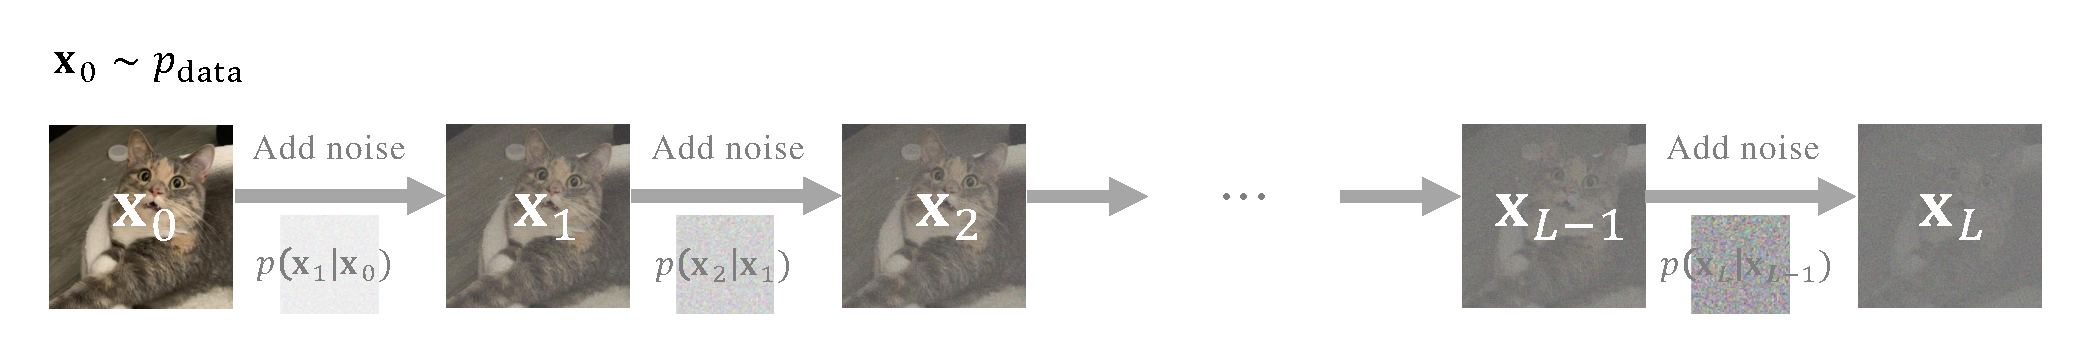
\includegraphics[width=\linewidth]{Images/PartB/vdm-forward.pdf}
    \caption{DDPM 前向过程的示意图，其中高斯噪声被逐步添加，将一个数据样本腐蚀为纯噪声。\figcredit{由作者绘制。}}
    \label{fig:vdm-forward}
\end{figure}

% \se{check indexing ranges below (from 0 or 1), seems off by one}

让我们将这种逐步退化形式化：
\paragraph{固定的高斯转移。}
前向过程中的每一步由一个固定的高斯转移核\footnote{这一表述虽然在形式上可能看起来不同，但在数学上等价于原始的 DDPM 转移核。}控制：
\[
p(\rvx_i|\rvx_{i-1}) := \mathcal{N}(\rvx_i; \sqrt{1 - \beta_i^2}   \rvx_{i-1}, \beta_i^2 \rmI).
\]
这里，过程从 $\rvx_{0} $ 开始，表示从真实数据分布 $p_{\text{data}}$ 中抽取的一个样本。序列 $\{\beta_i\}_{i=1}^L$ 表示一个预先确定的、单调递增的噪声调度，其中每个
$\beta_i \in (0, 1)$ 控制第 $i$ 步注入的高斯噪声的方差。为方便起见，我们定义 $\alpha_i := \sqrt{1 - \beta_i^2}$。这一定义与如下直观的迭代更新精确等价：
\[
\rvx_i = \alpha_i \rvx_{i-1} + \beta_i \bm{\epsilon}_i,  
\]
其中 $\bm{\epsilon}_i \sim \mathcal{N}(\bm{0}, \rmI)$ 是独立同分布的。这意味着在每一步 $i$，我们将前一状态 $\rvx_{i-1}$ 按 $\alpha_i$ 缩小，并添加一个由 $\beta_i$ 缩放的控制量的高斯噪声。

\paragraph{扰动核与先验分布。}
通过递归地应用转移核，我们得到了给定原始数据 $\rvx_0$ 时第 $i$ 步噪声样本分布的闭式表达式：
\[
p_i(\rvx_i|\rvx_0) = \mathcal{N}\left(\rvx_i; \bar{\alpha}_i \rvx_0, (1 - \bar{\alpha}_i^2) \rmI \right),
\]
其中
\[
\bar{\alpha}_i := \prod_{k=1}^i \sqrt{1-\beta_k^2} = \prod_{k=1}^i \alpha_k.
\]
这意味着我们可以直接从 $\rvx$ 采样 $\rvx_i$，如
\begin{align}\label{eq:ddpm-forward}
    \rvx_i = \bar{\alpha}_i \rvx_0 + \sqrt{1-\bar{\alpha}_i^2}   \bm{\epsilon}, \quad \bm{\epsilon} \sim \mathcal{N}(\bm{0}, \rmI).
\end{align}
令噪声调度 $ \{\beta_i\}_{i=1}^L $ 为一个递增序列，则前向过程的边际分布收敛为
\[
p_L(\mathbf{x}_L | \rvx_0) \longrightarrow \mathcal{N}(\mathbf{0}, \mathbf{I}) \quad \text{as } L \to \infty,
\]
这激发了对先验分布的选择
\[
p_{\text{prior}} := \mathcal{N}(\mathbf{0}, \mathbf{I})
\]
且不依赖于数据 $\rvx_0$。
% \paragraph{Marginal Densities.}
% By marginalizing over the data distribution using the law of total probability, the marginal density at step $i$ is
% \[
% p_i(\rvx_i) := \int p_i(\rvx_i|\rvx) p_{\text{data}}(\rvx_0) \diff \rvx_0.
% \]
% \se{what's the point of this paragraph?}


\subsection{反向去噪过程（可学习的解码器）}

% \se{this section packs too much content, too many formulas and will be overwhelming. since it is important, you need to break it up more and more gradually} \jcc{I cut the original section into 3 subsections: one is about oracle $p(\rvx_{i-1}|\rvx_i)$ and introduce high-level idea; the next subsection is about how to model $p_\bphi(\rvx_{i-1}|\rvx_i)$ with practical losses/parametrizations introduced there (\S 2.2.3); and the last one is Practical Choices of Predictions and Loss (\S 2.2.4). Also, I added some bridging and intuition.}

DDPM 的核心本质在于其\emph{反转}前向扩散过程所施加的受控退化的能力。从纯的、无结构的噪声 $\mathbf{x}_L \sim p_{\text{prior}}$ 出发，目标是逐步\emph{去噪}这种随机性，一步接一步，直到一个连贯而有意义的数据样本出现。这一反向生成通过一条马尔可夫链进行，如 \Cref{fig:ddpm-sampling-formal-rev} 所示。
\begin{figure}[tbh!]
    \centering
    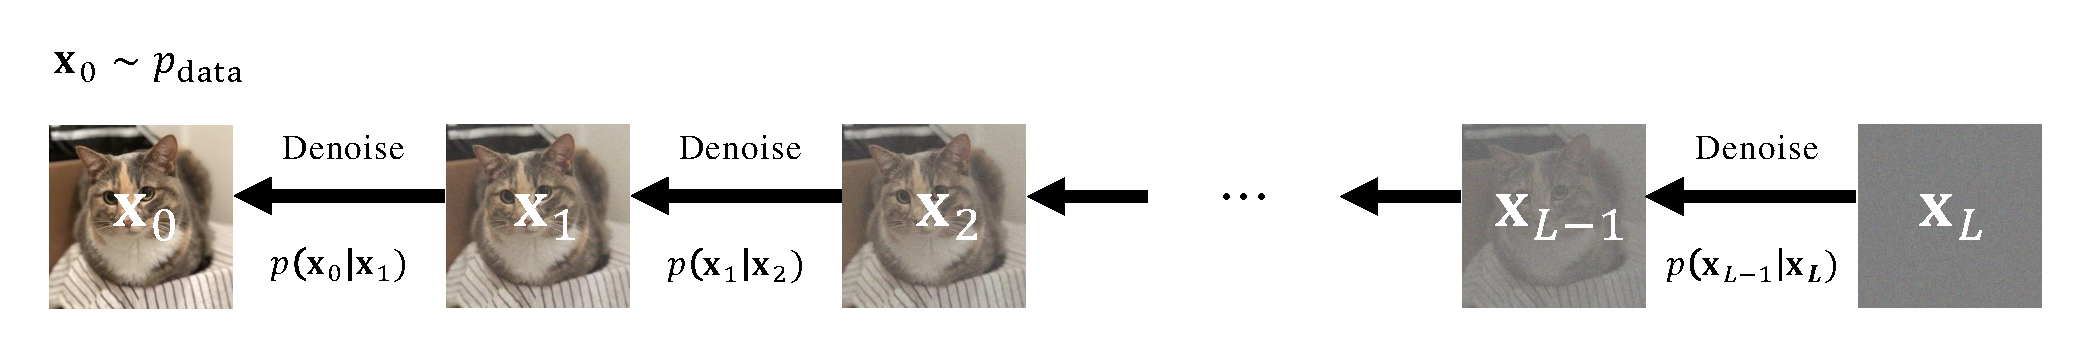
\includegraphics[width=\linewidth]{Images/PartB/vdm-backward.pdf}
\caption{\textbfs{DDPM 反向（去噪）过程示意图。}从噪声 $\mathbf{x}_L \sim  p_{\mathrm{prior}}$ 出发，模型依次采样 $\mathbf{x}_{i-1} \sim  p(\mathbf{x}_{i-1}|\mathbf{x}_i)$（$i=L,\ldots,1$）以获得新生成的数据 $\mathbf{x}_0$。先验的转移 $p(\mathbf{x}_{i-1}|\mathbf{x}_i)$ 是未知的；因此，我们的目标是近似它。
\figcredit{由作者绘制。}
}

    \label{fig:ddpm-sampling-formal-rev}
\end{figure}





那么，指导 DDPM 发展的根本挑战和核心问题就变成：
\begin{question}
我们能否精确计算，或至少有效地近似这些反向转移核 $ p(\mathbf{x}_{i-1}|\mathbf{x}_i) $，尤其是在考虑 $\mathbf{x}_i \sim p_i(\mathbf{x}_i)$ 的复杂分布时？
\end{question}

我们不立即深入证据下界（ELBO）的数学上错综复杂的推导（正如原始 DDPM 论文所做的，其详细讨论留待 \Cref{subsec:ddpm-elbo}），而是从一个更直观的视角来处理训练目标：利用条件概率来获得一个可处理的表述。


\paragraph{概述：建模与训练目标。} 
为了实现生成过程，我们的目标是近似未知的真实反向转移核 $p(\mathbf{x}_{i-1}|\mathbf{x}_i)$。我们通过引入一个可学习的参数化模型 $p_{\bm{\phi}}(\mathbf{x}_{i-1}|\mathbf{x}_i)$，并训练它以最小化期望 KL 散度来实现这一点：
\begin{align}\label{eq:marginal-kl-matching}
    \mathbb{E}_{p_i(\mathbf{x}_i)} \left[
    \mathcal{D}_{\mathrm{KL}}\big(p(\mathbf{x}_{i-1}|\mathbf{x}_i) \| p_{\bm{\phi}}(\mathbf{x}_{i-1}|\mathbf{x}_i)\big)
    \right].
\end{align}

然而，对目标分布 $p(\mathbf{x}_{i-1}|\mathbf{x}_i)$ 的直接计算具有挑战性。由贝叶斯定理，我们需要计算：
\[
p(\mathbf{x}_{i-1}|\mathbf{x}_i) = p(\mathbf{x}_i|\mathbf{x}_{i-1}) \underbrace{\frac{p_{i-1}(\mathbf{x}_{i-1})}{p_i(\mathbf{x}_i)}}_{\text{intractable}}.
\]
边际分布 $p_i(\rvx_i)$ 和 $p_{i-1}(\rvx_{i-1})$ 是对未知数据分布 $p_{\mathrm{data}}$ 的期望，由下式给出：
\[
p_i(\rvx_i) = \int p_i(\rvx_i | \rvx_0) p_{\mathrm{data}}(\rvx_0) \mathrm{d}\rvx_0,
\]
$p_{i-1}(\rvx_{i-1})$ 类似。由于 $p_{\mathrm{data}}$ 未知，这些积分没有闭式求值；充其量只能用样本来近似，因此实践中无法得到精确的密度。

\begin{figure}[th!]
    \centering
    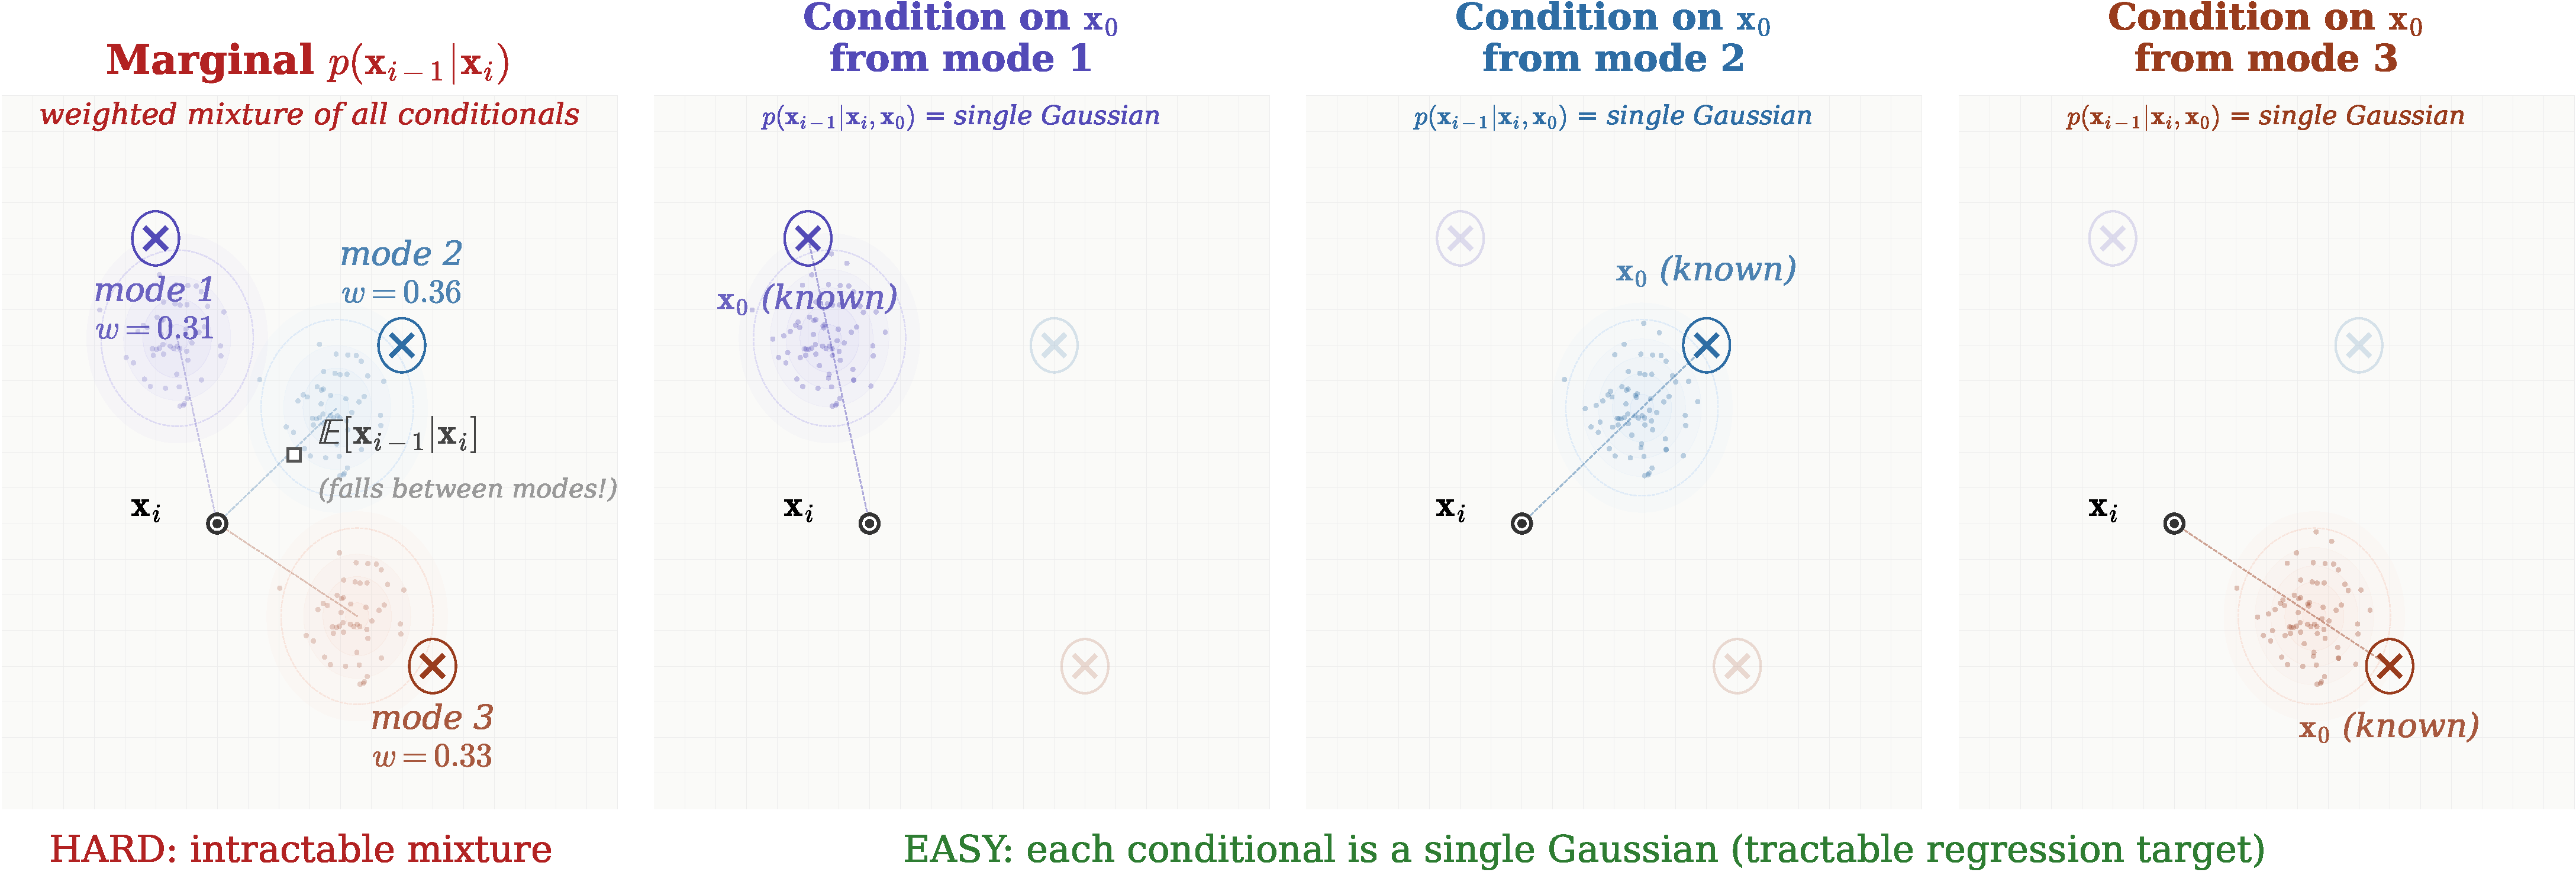
\includegraphics[width=\linewidth]{Images/PartB/ddpm_conditional_trick.pdf}
    \caption{\textbfs{DDPM 中条件化技巧的示意图。}
对于一个固定的噪声样本 $\rvx_i$，真实的反向分布
$p(\rvx_{i-1}|\rvx_i)$ 是通过对所有可能的干净来源 $\rvx_0$ 边际化诱导的，因此通常是一个可能是多峰的混合分布。
它的均值甚至可能落在模式之间，使得直接预测变得困难。
相比之下，一旦我们对干净样本 $\rvx_0$ 进行条件化，反向后验
$p(\rvx_{i-1}|\rvx_i,\rvx_0)$ 就变成单个高斯分布。
DDPM 在训练中利用了这一可处理的条件结构，用一个可处理的回归目标代替了困难的多峰预测问题。\figcredit{由作者在 AI 辅助编程下绘制。}}
    \label{fig:conditional-trick}
\end{figure}


\paragraph{用条件化克服不可处理性。}
DDPM 中的一个核心洞察解决了这一不可处理性：我们用干净的数据样本 $\mathbf{x}_0$ 对反向转移进行条件化。这一微妙却有力的步骤将不可处理的核转化为一个数学上可处理的核：
\[
p(\mathbf{x}_{i-1}|\mathbf{x}_i, \mathbf{x}_0) = p(\mathbf{x}_i|\mathbf{x}_{i-1}) \frac{p(\mathbf{x}_{i-1}|\mathbf{x}_0)}{p(\mathbf{x}_i|\mathbf{x}_0)}.
\]
这一可处理性源于前向过程的两个关键性质：其马尔可夫性质，即 $p(\mathbf{x}_i|\mathbf{x}_{i-1}, \mathbf{x}_0) = p(\mathbf{x}_i|\mathbf{x}_{i-1})$，以及所有相关分布的高斯性质。因此，$p(\mathbf{x}_{i-1}|\mathbf{x}_i, \mathbf{x}_0)$ 本身是高斯的，并具有闭式表达式（我们将在 \Cref{eq:ddpm-reverse-mean} 中看到）。我们在 \Cref{fig:conditional-trick} 中对其进行了可视化。关键的是，这种优雅的条件化策略使我们能够推导出一个可处理的目标，它在功能上等价于 \Cref{eq:marginal-kl-matching} 中看似不可处理的边际 KL 散度。

\thmp{边际 KL 与条件 KL 最小化的等价性}{equiv-marginal-kl}{
如下等式成立：
\begin{align}\label{eq:kl-matching}
\begin{aligned}
    &\mathbb{E}_{p_i(\rvx_i)}\left[
        \mathcal{D}_{\mathrm{KL}}\big(p(\rvx_{i-1}|\rvx_i) \| p_{\bm{\phi}}(\rvx_{i-1}|\rvx_i)\big)
    \right] \\
    ={}&
    \mathbb{E}_{p_{\mathrm{data}}(\rvx_0)}
    \mathbb{E}_{p(\rvx_i|\rvx_0)} \left[
        \mathcal{D}_{\mathrm{KL}}\big(p(\rvx_{i-1}|\rvx_i, \rvx_0) \| p_{\bm{\phi}}(\rvx_{i-1}|\rvx_i)\big)
    \right] + C.
\end{aligned}
\end{align}
其中 $C$ 是与 $\bm{\phi}$ 无关的常数。此外，\Cref{eq:kl-matching} 的最小化子满足
\[
p^*(\mathbf{x}_{i-1}|\mathbf{x}_i) = \mathbb{E}_{p(\mathbf{x}_0|\mathbf{x}_i)} \big[p(\mathbf{x}_{i-1}|\mathbf{x}_i, \mathbf{x}_0)\big] = p(\mathbf{x}_{i-1}|\mathbf{x}_i), \quad \mathbf{x}_i \sim p_i.
\]
}{证明通过展开定义、应用概率的链式法则，并利用一个对数恒等式，将一个 KL 散度期望重写为一个期望条件 KL 散度与一个边际 KL 散度之和。完整的推导见 \Cref{subsec:proof-equiv-marginal-kl}。}


这一替代视角——通过条件化获得一个可处理的目标——构成了 DDPM 的基础，并揭示了与其他有影响力的扩散模型的深刻共性，正如我们将在 \Cref{ch:score-based} 和 \Cref{ch:flow-based} 中探讨的那样。


它揭示了一个有力的等价性：最小化边际分布之间的 KL 散度在数学上等价于最小化特定条件分布之间的 KL 散度。后一种表述异常有用，因为关键的条件分布 $p(\mathbf{x}_{i-1}|\mathbf{x}_i, \mathbf{x})$ 具有一个方便的闭式表达式：
\lem{反向条件转移核}{ddpm-reverse-kernel}{$p(\mathbf{x}_{i-1} | \mathbf{x}_i, \mathbf{x})$ 是高斯分布，具有如下闭式表达式：
\begin{align*}
    p(\rvx_{i-1} | \rvx_i, \rvx) =\mathcal{N}\left(\rvx_{i-1}; \bm{\mu}\left(\rvx_i, \rvx, i\right), \sigma^2(i)\rmI \right),
\end{align*}
其中
\begin{align}\label{eq:ddpm-reverse-mean}
\begin{aligned}
            \bm{\mu}\left(\rvx_i, \rvx, i\right):= \frac{\bar{\alpha}_{i-1}\beta_i^2}{1-\bar{\alpha}_i^2}\rvx + \frac{(1-\bar{\alpha}_{i-1}^2)\alpha_i }{1-\bar{\alpha}_i^2}\rvx_i,
\quad  \sigma^2(i) := \frac{1-\bar{\alpha}_{i-1}^2}{1-\bar{\alpha}_i^2}\beta_i^2.
\end{aligned}
\end{align}
}
在后面的引理~\ref{reverse-kernel} 中，我们给出了一个更通用的公式，它超越了 \Cref{eq:ddpm-forward} 中描述的 DDPM 加噪过程。


\subsection{反向转移核 $p_{\bm{\phi}}(\mathbf{x}_{i-1}|\mathbf{x}_i)$ 的建模} 利用定理~\ref{thm:equiv-marginal-kl} 中梯度层面的等价性以及引理~\ref{ddpm-reverse-kernel} 中反向条件 $p(\mathbf{x}_{i-1}|\mathbf{x}_i, \mathbf{x})$ 的高斯形式，DDPM 假设每个反向转移 $p_{\bm{\phi}}(\rvx_{i-1}| \rvx_i)$ 是高斯的，参数化为
\begin{align}\label{eq:def-reverse}
    p_{\bm{\phi}}(\mathbf{x}_{i-1}|\mathbf{x}_i) := \mathcal{N}\big(\mathbf{x}_{i-1}; \bm{\mu}_{\bm{\phi}}(\mathbf{x}_i, i), \sigma^2(i) \mathbf{I}\big),
\end{align}
其中 $\bm{\mu}_{\bm{\phi}}(\cdot, i) \colon \mathbb{R}^D \to \mathbb{R}^D$ 是一个可学习的均值函数，$\sigma^2(i) > 0$ 固定为 \Cref{eq:ddpm-reverse-mean} 中所定义。

我们将时间步 $i$ 上取平均、以数据 $\rvx_0 \sim p_{\text{data}}$ 为条件的 KL 散度记为匹配所有层分布：
\begin{align}\label{eq:ddpm-diffusion}
    \mathcal{L}_{\text{diffusion}}(\rvx_0;\bm{\phi}) := \sum_{i=2}^L \mathbb{E}_{p(\rvx_i|\rvx_0)}\left[\mathcal{D}_{\text{KL}}\big(p(\rvx_{i-1}|\rvx_i, \rvx_0)  \Vert  p_{\bm{\phi}}(\rvx_{i-1}|\rvx_i)\big)\right].
\end{align}
由于两个分布都是高斯的，且采用 \Cref{eq:def-reverse} 中定义的参数化，该目标具有闭式表达式，并可简化为：
\begin{align}\label{eq:ddpm-diffusion-simp}
    \mathcal{L}_{\text{diffusion}}(\rvx_0;\bm{\phi}) = \sum_{i=2}^L \frac{1}{2\sigma^2(i)}  \mathbb{E}_{p(\rvx_i|\rvx_0)}\left\| \bm{\mu}_{\bm{\phi}}(\rvx_i, i) - \bm{\mu}(\rvx_i, \rvx_0, i) \right\|_2^2 + C,
\end{align}
其中 $C$ 是与 $\bm{\phi}$ 无关的常数。对数据分布取平均并省略常数 $C$（它不影响优化），最终的 DDPM 训练目标为
\begin{align}
\begin{aligned}
    \label{eq:ddpm-mean-loss}
    \mathcal{L}_{\text{DDPM}}(\bm{\phi}) := \sum_{i=2}^L \frac{1}{2\sigma^2(i)}  \mathbb{E}_{\rvx_0} \mathbb{E}_{p(\mathbf{x}_i|\rvx_0)} \left[ \left\| \bm{\mu}_{\bm{\phi}}(\mathbf{x}_i, i) - \bm{\mu}(\mathbf{x}_i, \rvx_0, i) \right\|_2^2 \right],
\end{aligned}
\end{align}
其中 $\rvx_0\sim p_{\mathrm{data}}$。

\subsection{预测与损失的实际选择}\label{subsec:ddpm-prediction}

\paragraph{$\beps$-预测。}
在典型的 DDPM 实现中，训练并不直接使用 \Cref{eq:ddpm-mean-loss} 中基于\emph{均值预测}参数化的原始损失。相反，通常采用一种等价的重参数化，即\emph{$\beps$-预测}（噪声预测）形式。

回想在 DDPM 前向过程中，噪声水平 $i$ 处的一个噪声样本 $\rvx_i \sim p(\rvx_i |\rvx_0)$ 通过下式生成
\begin{equation}\label{eq:ddpm-perturbation}
    \rvx_i = \bar{\alpha}_i \rvx_0 + \sqrt{1 - \bar{\alpha}_i^2}   \boldsymbol{\epsilon}, \quad \rvx_0 \sim p_{\text{data}}, \quad \boldsymbol{\epsilon} \sim \mathcal{N}(\mathbf{0}, \mathbf{I}).
\end{equation}
利用这一表达式，\Cref{eq:ddpm-reverse-mean} 中的反向均值 $\bm{\mu}(\rvx_i, \rvx_0, i)$ 可以重写为：
\[
\bm{\mu}(\rvx_i, \rvx_0, i) = \frac{1}{\alpha_i} \left( \rvx_i - \frac{1 - \alpha_i^2}{\sqrt{1 - \bar{\alpha}_i^2}} \boldsymbol{\epsilon} \right).
\]

这激发了对模型均值 $\bm{\mu}_{\bm{\phi}}$ 的一种参数化，使用一个直接预测噪声的神经网络 $\boldsymbol{\epsilon}_{\bm{\phi}}(\rvx_i, i)$：
\[
\bm{\mu}_{\bm{\phi}}(\rvx_i, i) = \frac{1}{\alpha_i} \left( \rvx_i - \frac{1 - \alpha_i^2}{\sqrt{1 - \bar{\alpha}_i^2}} \underbrace{\boldsymbol{\epsilon}_{\bm{\phi}}(\rvx_i, i)}_{\beps\text{-prediction}} \right).
\]
将其代入原始损失，得到预测噪声与真实噪声之间的一个平方 $\ell_2$ 误差：
\[
\left\| \bm{\mu}_{\bm{\phi}}(\rvx_i, i) - \bm{\mu}(\rvx_i, \rvx_0, i) \right\|_2^2 \propto \left\| \boldsymbol{\epsilon}_{\bm{\phi}}(\rvx_i, i) - \boldsymbol{\epsilon} \right\|_2^2,
\]
至多差一个依赖于 $i$ 的加权因子。直观地说，模型扮演“噪声侦探”的角色，估计前向过程中每一步添加的随机噪声。从被腐蚀的样本中减去这一估计，会使其更接近干净的原始样本，而一步一步地重复这一过程就从纯噪声中重建出数据。

\paragraph{带有 $\beps$-预测的简化损失。}
在实践中，这一表达式通过省略加权项被进一步简化，得到广泛使用的 DDPM 训练损失：
\begin{equation}\label{eq:ddpm-simple-loss}
    \mathcal{L}_{\text{simple}}(\bm{\phi}) := \mathbb{E}_{i} \mathbb{E}_{\rvx \sim p_{\text{data}}(\rvx)} \mathbb{E}_{\boldsymbol{\epsilon} \sim \mathcal{N}(\mathbf{0}, \mathbf{I})} \left[ \left\| \boldsymbol{\epsilon}_{\bm{\phi}}(\rvx_i, i) - \boldsymbol{\epsilon} \right\|_2^2 \right],
\end{equation}
其中 $\rvx_i = \bar{\alpha}_i \rvx_0 + \sqrt{1 - \bar{\alpha}_i^2} \boldsymbol{\epsilon}$，$\rvx_0 \sim p_{\text{data}}$。由于目标噪声在每个时间步 $t$ 都具有单位方差，\Cref{eq:ddpm-simple-loss} 中的 $\ell_2$ 损失在所有 $t$ 上保持一致的尺度。这防止了目标的消失或爆炸，并消除了显式损失加权的需要。


重要的是，$\mathcal{L}_{\text{DDPM}}$ 和 $\mathcal{L}_{\text{simple}}$ 共享相同的最优解 $\boldsymbol{\epsilon}^*$，这是因为 \Cref{eq:ddpm-simple-loss} 本质上退化为一个最小二乘问题（类似地如命题~\ref{dsm-minimizer} 或命题~\ref{equi-para} 所示）：
\[
\boldsymbol{\epsilon}^*(\rvx_i, i) = \mathbb{E}\left[ \boldsymbol{\epsilon}|\rvx_i \right], \quad \rvx_i \sim p_i.
\]
直观地说，$\beps$-预测网络 $\boldsymbol{\epsilon}_{\bm{\phi}}(\rvx_i, i)$ 估计前向过程为产生 $\rvx_i$ 而添加的噪声。在最优时，这一估计与真实噪声的条件期望一致，尽管 $\rvx_i$ 并不唯一地确定原始干净样本。

\paragraph{另一种等价的参数化：$\rvx$-预测。}
\Cref{eq:ddpm-reverse-mean} 启发了一种替代但等价的参数化，称为\emph{$\rvx$-预测}（干净预测），其中一个神经网络 $\rvx_{\bm{\phi}}(\rvx_i, i)$ 被训练以从给定的噪声输入 $\rvx_i \sim p_i(\rvx_i)$ 在噪声水平 $i$ 处预测一个干净（去噪）样本。将反向均值表达式中的真实干净样本 $\rvx_0$ 替换为 $\rvx_{\bm{\phi}}(\rvx_i, i)$ 得到如下模型：
\begin{align*}
\bm{\mu}_{\bm{\phi}}(\rvx_i, i) = \frac{\bar{\alpha}_{i-1} \beta_i^2}{1 - \bar{\alpha}_i^2} \rvx_{\bm{\phi}}(\rvx_i, i) + \frac{(1 - \bar{\alpha}_{i-1}^2)\alpha_i}{1 - \bar{\alpha}_i^2} \rvx_i.
\end{align*}
类似于 $\beps$-预测形式，训练目标可以表示为
\[
\left\| \bm{\mu}_{\bm{\phi}}(\rvx_i, i) - \bm{\mu}(\rvx_i, \rvx_0, i) \right\|_2^2 \propto \left\| \rvx_{\bm{\phi}}(\rvx_i, i) - \rvx_0 \right\|_2^2, \quad \rvx_0 \sim p_{\text{data}},
\]
其中模型被训练以从其噪声版本 $\rvx_i$ 预测原始数据样本 $\rvx_0$。这一等价性将 \Cref{eq:ddpm-mean-loss} 中的均值匹配损失简化为
\[
\mathbb{E}_{i} \mathbb{E}_{\rvx_0 \sim p_{\text{data}}} \mathbb{E}_{\boldsymbol{\epsilon} \sim \mathcal{N}(\mathbf{0}, \mathbf{I})} \left[\omega_i \left\| \rvx_{\bm{\phi}}(\rvx_i, i) - \rvx_0 \right\|_2^2 \right],
\]
对某个加权函数 $\omega_i$。由于这是一个最小二乘问题，最优解由（见命题~\ref{dsm-minimizer} 或命题~\ref{equi-para}）
\begin{align}\label{eq:ddpm-clean-minimizer}
    \rvx^*(\rvx_i, i) = \mathbb{E}\left[ \rvx_0|\rvx_i \right], \quad \rvx_i \sim p_i,
\end{align}
给出，即模型应在时间步 $i$ 给定噪声观测 $\rvx_i$ 时预测期望的干净数据。

$\rvx$-预测和 $\beps$-预测参数化在数学上是等价的，并通过前向过程联系起来：
\begin{equation}\label{eq:ddpm-clean-noise}
    \rvx_i = \bar{\alpha}_i \rvx_{\bm{\phi}}(\rvx_i, i) + \sqrt{1 - \bar{\alpha}_i^2}   \boldsymbol{\epsilon}_{\bm{\phi}}(\rvx_i, i).
\end{equation}
也就是说，人们既可以预测干净样本 $\rvx_{\bm{\phi}}(\rvx_i, i)$，也可以预测噪声 $\boldsymbol{\epsilon}_{\bm{\phi}}(\rvx_i, i)$，使得它们的组合在前向加噪过程下重现 $\rvx_i$。 




\subsection{DDPM 的 ELBO}\label{subsec:ddpm-elbo} 将反向转移如 \Cref{eq:def-reverse} 中那样定义后，这导出了 DDPM 中联合生成分布的定义：
\[
p_{\bm{\phi}}(\rvx_0, \rvx_{1:L}) := p_{\bm{\phi}}(\rvx_0|\rvx_1)  p_{\bm{\phi}}(\rvx_1|\rvx_2)\cdots p_{\bm{\phi}}(\rvx_{L-1}|\rvx_L)   p_{\text{prior}}(\rvx_L),
\]
而数据的边际生成模型由下式给出：
\begin{align*}
    p_{\bm{\phi}}(\rvx_0) := \int p_{\bm{\phi}}(\rvx_0, \rvx_{1:L}) \diff \rvx_{1:L}.
\end{align*}

事实上，通过 \Cref{eq:ddpm-diffusion} 进行的 DDPM 训练可以严格地建立在极大似然估计（\Cref{eq:MLE}）之上。具体而言，其目标构成一个 ELBO，类似于 \Cref{sec:vae} 中 VAE 和 HVAE 的 ELBO，它作为对数密度的下界：
\thmp{DDPM 的 ELBO}{ddpm-elbo}{    
\begin{align}\label{eq:ddpm-elbo}
        \begin{aligned}
        -\log p_{\bm{\phi}}(\rvx_0)  &\leq-\mathcal{L}_{\text{ELBO}}(\rvx_0; \bm{\phi}) 
        \\&:= \mathcal{L}_{\text{prior}}(\rvx_0) + \mathcal{L}_{\text{recon.}}(\rvx_0;\bm{\phi})  + \mathcal{L}_{\text{diffusion}}(\rvx_0;\bm{\phi})
        \end{aligned}
\end{align}
这里，损失的每个分量定义为：
\begin{align*}
   \mathcal{L}_{\text{prior}}(\rvx_0) &:= \mathcal{D}_{\text{KL}}\Big( p(\rvx_L|\rvx_0) \Vert p_{\text{prior}}(\rvx_L)\Big)\\
   \mathcal{L}_{\text{recon.}}(\rvx_0;\bm{\phi}) &:= \mathbb{E}_{p(\rvx_1|\rvx_0)}\left[-\log p_{\bm{\phi}}(\rvx_0|\rvx_1)\right]\\
   \mathcal{L}_{\text{diffusion}}(\rvx_0;\bm{\phi}) &= \sum_{i=2}^L  \mathbb{E}_{p(\rvx_i|\rvx_0)}\left[\mathcal{D}_{\text{KL}}\Big(p(\rvx_{i-1}|\rvx_i, \rvx_0) \Vert p_{\bm{\phi}}(\rvx_{i-1}|\rvx_i) \Big)\right]. 
\end{align*}}{该推导应用了 Jensen 不等式，如同 HVAE/VAE 的 ELBO（\Cref{eq:hvae-elbo}），并作了进一步简化。详细证明留待 \Cref{app:vlb-proof}。
}
ELBO $\mathcal{L}_{\text{ELBO}}$ 由三项组成：
\begin{itemize}
    \item $\mathcal{L}_{\text{prior}}$ 可以通过选择噪声调度 $\{\beta_i\}$ 使得 $p(\cdot|\rvx_0) \approx p_{\text{prior}}(\cdot)$ 而变得可忽略。
    \item 对于 $\mathcal{L}_{\text{recon.}}$，可以用蒙特卡洛估计来近似和优化；实际实现见 \citep{ho2020denoising, kingma2021variational}。
    \item $\mathcal{L}_{\text{diffusion}}$（参见 \Cref{eq:ddpm-diffusion}）在所有步骤 $i$ 上将反向条件分布 $p_{\bm{\phi}}(\mathbf{x}_{i-1}|\mathbf{x}_i)$ 匹配到 $p(\mathbf{x}_{i-1}|\mathbf{x}_i)$。
\end{itemize}

ELBO 目标 $\mathcal{L}_{\text{ELBO}}$ 也可以通过带有隐变量 $\rvz = \rvx_{1:L}$ 的数据处理不等式视角来解释，如 \Cref{eq:joint-bound} 所示：
\begin{align*}
    \mathcal{D}_{\mathrm{KL}}(p_{\mathrm{data}}(\rvx_0) \| p_{\bm{\phi}}(\rvx_0)) \leq \mathcal{D}_{\mathrm{KL}}\left(p(\rvx_0, \rvx_{1:L}) \| p_{\bm{\phi}}(\rvx_0, \rvx_{1:L})\right),
\end{align*}
其中 $p(\rvx_0, \rvx_{1:L}) := p_{\mathrm{data}}(\rvx_0)  p(\rvx_1|\rvx_0)  p(\rvx_2|\rvx_1) \cdots p(\rvx_L|\rvx_{L-1})$ 表示沿前向过程的联合分布。 




\rmkb{扩散模型的变分视角契合 HVAE 模板：“编码器”是固定的前向加噪链，隐变量 $\mathbf{x}_{1:T}$ 与数据共享维度。训练最大化同一个 ELBO。这里没有学习得到的编码器，也没有逐层的 KL 项；相反，目标分解为从大到小噪声（由粗到细）的良好条件化的去噪子问题，从而产生稳定的优化和较高的样本质量，同时沿时间/噪声保留了一个由粗到细的层次。
 }





\subsection{采样}
在训练好 $\beps$-预测模型 $\bm{\epsilon}_{\bm{\phi}^\times}(\rvx_i, i)$\footnote{我们使用符号“$\times$”来表示模型已经训练完毕且现在被冻结。}之后，采样如 \Cref{fig:ddpm-sampling-formal-rev} 所示顺序进行，使用参数化的转移 $p_{\bm{\phi}^\times}(\rvx_{i-1} | \rvx_i)$。


更具体地说，从一个随机种子 $\rvx_L \sim p_{\text{prior}} = \mathcal{N}(\bm{0},\rmI)$ 出发，我们对 $i = L, L-1, \dots, 1$ 按照如下更新规则从 $p_{\bm{\phi}^\times}(\rvx_{i-1} | \rvx_i)$ 递归地采样：
\begin{align}\label{eq:ddpm-sampling}
    \rvx_{i-1} \leftarrow \underbrace{\frac{1}{\alpha_i}\left( \rvx_i  - \frac{1-\alpha_i^2}{\sqrt{1-\bar{\alpha}_i^2}} \bm{\epsilon}_{\bm{\phi}^\times}(\rvx_i, i)\right)}_{\bm{\mu}_{\bm{\phi}^\times}(\rvx_i, i)} +\sigma(i) \bm{\epsilon}_i,\quad \bm{\epsilon}_i\sim  \mathcal{N}(\bm{0},\rmI).
\end{align}
这一“去噪”过程持续进行，直到获得 $\rvx_0$ 作为最终的干净生成样本。 



% \paragraph{Another Interpretation of DDPM's Sampling.} From \Cref{eq:ddpm-clean-noise}, the clean sample prediction corresponding to a noise estimate $\boldsymbol{\epsilon}_{\bm{\phi}^\times}(\rvx_i, i)$ can be expressed as
% \[
% \rvx_{\bm{\phi}^\times}(\rvx_i, i) = \frac{\rvx_i - \sqrt{1 - \bar{\alpha}_i^2}   \boldsymbol{\epsilon}_{\bm{\phi}^\times}(\rvx_i, i)}{\bar{\alpha}_i}.
% \]
% Plugging this into the DDPM sampling rule in \Cref{eq:ddpm-sampling} yields the equivalent update:
% \[
% \rvx_{i-1} \leftarrow \text{(interpolation between $\rvx_i$ and clean prediction $\rvx_{\bm{\phi}^\times}$)} + \sigma(i) \boldsymbol{\epsilon}_i
% \]
% indicating that each step is centered around the predicted clean sample, with added Gaussian noise scaled by $\sigma(i)$.

% \paragraph{Another Interpretation of DDPM Sampling.}
% A useful way to interpret DDPM sampling is to rewrite the predicted noise in terms of the current sample $\rvx_i$ and the predicted clean sample $\rvx_{\bm{\phi}^\times}(\rvx_i,i)$. From \Cref{eq:ddpm-clean-noise},
% \[
% \boldsymbol{\epsilon}_{\bm{\phi}^\times}(\rvx_i,i)
% =
% \frac{\rvx_i-\bar{\alpha}_i\,\rvx_{\bm{\phi}^\times}(\rvx_i,i)}{\sqrt{1-\bar{\alpha}_i^2}}.
% \]
% Substituting this expression into the DDPM sampling rule in \Cref{eq:ddpm-sampling} gives
% \[
% \rvx_{i-1}
% \leftarrow
% \underset{\text{interpolation between $\rvx_i$ and clean prediction $\rvx_{\bm{\phi}^\times}$}}{\underbrace{\frac{\alpha_i(1-\bar{\alpha}_{i-1}^2)}{1-\bar{\alpha}_i^2}\,\rvx_i
% +
% \frac{\bar{\alpha}_{i-1}\beta_i^2}{1-\bar{\alpha}_i^2}\,\rvx_{\bm{\phi}^\times}(\rvx_i,i)
% }}
% +
% \sigma(i)\,\boldsymbol{\epsilon}_i.
% \]
% Thus, the mean of the DDPM update is an interpolation between the current noisy sample $\rvx_i$ and the predicted clean sample $\rvx_{\bm{\phi}^\times}(\rvx_i,i)$, followed by Gaussian perturbation with scale $\sigma(i)$.

% This reveals that DDPM sampling can be viewed as an iterative denoising process that alternates between:
% \begin{enumerate}
%     \item Estimating the clean data $\mathbf{x}_{\bm{\phi}^\times}(\mathbf{x}_i, i)$ from the current noisy input $\mathbf{x}_i$,
%     \item Sampling a less noisy latent $\mathbf{x}_{i-1}$ via the update rule using this clean estimate.
% \end{enumerate}



% However, even if $\mathbf{x}_{\bm{\phi}^\times}$ is trained as the optimal denoiser (i.e., the conditional expectation minimizer; see \Cref{eq:ddpm-clean-minimizer}), it can only predict the \emph{average} clean sample given $\rvx_i$. This limitation leads to blurry predictions, particularly at high noise levels, where recovering detailed structure from severely corrupted inputs becomes difficult.


% From this viewpoint, diffusion sampling typically moves from high to low noise and progressively refines an estimate of the clean signal. Early steps set the global structure, later steps add fine detail, and the sample becomes more realistic as the noise is removed.


\paragraph{DDPM 采样的另一种解释。}

解释 DDPM 采样的一种有用方式是重写更新规则
使噪声水平的结构变得显式。
回想 \Cref{eq:ddpm-clean-noise}，预测噪声可以用
当前样本 $\rvx_i$ 和预测的
干净样本 $\rvx_{\bm{\phi}^\times}(\rvx_i,i)$ 表示为：
\[
\boldsymbol{\epsilon}_{\bm{\phi}^\times}(\rvx_i,i)
=
\frac{\rvx_i - \bar{\alpha}_i\,\rvx_{\bm{\phi}^\times}(\rvx_i,i)}
     {\sqrt{1-\bar{\alpha}_i^2}}.
\]
将其代入 DDPM 采样规则
（\Cref{eq:ddpm-sampling}）并整理，我们得到
\begin{equation}\label{eq:ddpm-renoise}
\rvx_{i-1}
\;\leftarrow\;
\bar{\alpha}_{i-1}\,\rvx_{\bm{\phi}^\times}(\rvx_i,i)
\;+\;
\underbrace{
  \sqrt{1-\bar{\alpha}_{i-1}^2 - \tilde{\beta}_i^2}\;
  \boldsymbol{\epsilon}_{\bm{\phi}^\times}(\rvx_i,i)
  \;+\;
  \tilde{\beta}_i\,\boldsymbol{\epsilon}_i
}_{\text{combined std.\ }=\;\sqrt{1-\bar{\alpha}_{i-1}^2}},
\end{equation}
其中 $\tilde{\beta}_i^2
= \frac{(1-\bar{\alpha}_{i-1}^2)(1-\alpha_i^2)}{1-\bar{\alpha}_i^2}$
是 DDPM 后验方差\footnote{%
系数
$\sqrt{1-\bar{\alpha}_{i-1}^2 - \tilde{\beta}_i^2}$
简化为
$\frac{\alpha_i(1-\bar{\alpha}_{i-1}^2)}{\sqrt{1-\bar{\alpha}_i^2}}$，
它始终非负，因此平方根是良好定义的。}。
此外，残差系数满足
\[
\bigl(1-\bar{\alpha}_{i-1}^2-\tilde{\beta}_i^2\bigr)+\tilde{\beta}_i^2
=
1-\bar{\alpha}_{i-1}^2,
\]
因此更新具有与前向过程在水平 $i-1$ 处相同的噪声水平结构。

将 \Cref{eq:ddpm-renoise} 与前向边际
$\rvx_{i-1} = \bar{\alpha}_{i-1}\,\rvx_0
+ \sqrt{1-\bar{\alpha}_{i-1}^2}\,\bar{\boldsymbol{\epsilon}}$ 比较。
结构是相同的：信号系数 $\bar{\alpha}_{i-1}$
和噪声标准差 $\sqrt{1-\bar{\alpha}_{i-1}^2}$，
只是未知的 $\rvx_0$ 被网络
预测 $\rvx_{\bm{\phi}^\times}(\rvx_i,i)$ 所代替。
换言之，每个 DDPM 步骤都\emph{预测干净数据，
然后将其重新加噪至恰好噪声水平 $i{-}1$}。
因此，可以将 DDPM 采样视为迭代两个操作：
\begin{enumerate}
    \item \textbfs{去噪。}
          从当前噪声输入 $\rvx_i$ 估计干净数据
          $\rvx_{\bm{\phi}^\times}(\rvx_i, i)$。
    \item \textbfs{重新加噪。}
          通过 \Cref{eq:ddpm-renoise} 在降低的水平 $i{-}1$
          处加回噪声，
          产生一个噪声水平与前向过程在步骤 $i{-}1$ 处相匹配的样本 $\rvx_{i-1}$。
\end{enumerate}


然而，即使 $\rvx_{\bm{\phi}^\times}$ 被训练为最优
去噪器（即条件期望最小化子；
见 \Cref{eq:ddpm-clean-minimizer}），它在给定 $\rvx_i$ 时也只能预测
\emph{平均}的干净样本。
这一局限导致模糊的预测，尤其是在高
噪声水平下，此时从严重腐蚀
的输入中恢复精细结构变得困难。
从这个角度看，扩散采样从高噪声移动到低噪声
并逐步细化对干净信号的估计。
早期步骤设定全局结构，后期步骤添加精细细节，
而样本随着噪声被去除变得越来越逼真。



\begin{figure}[th!]
    \centering
    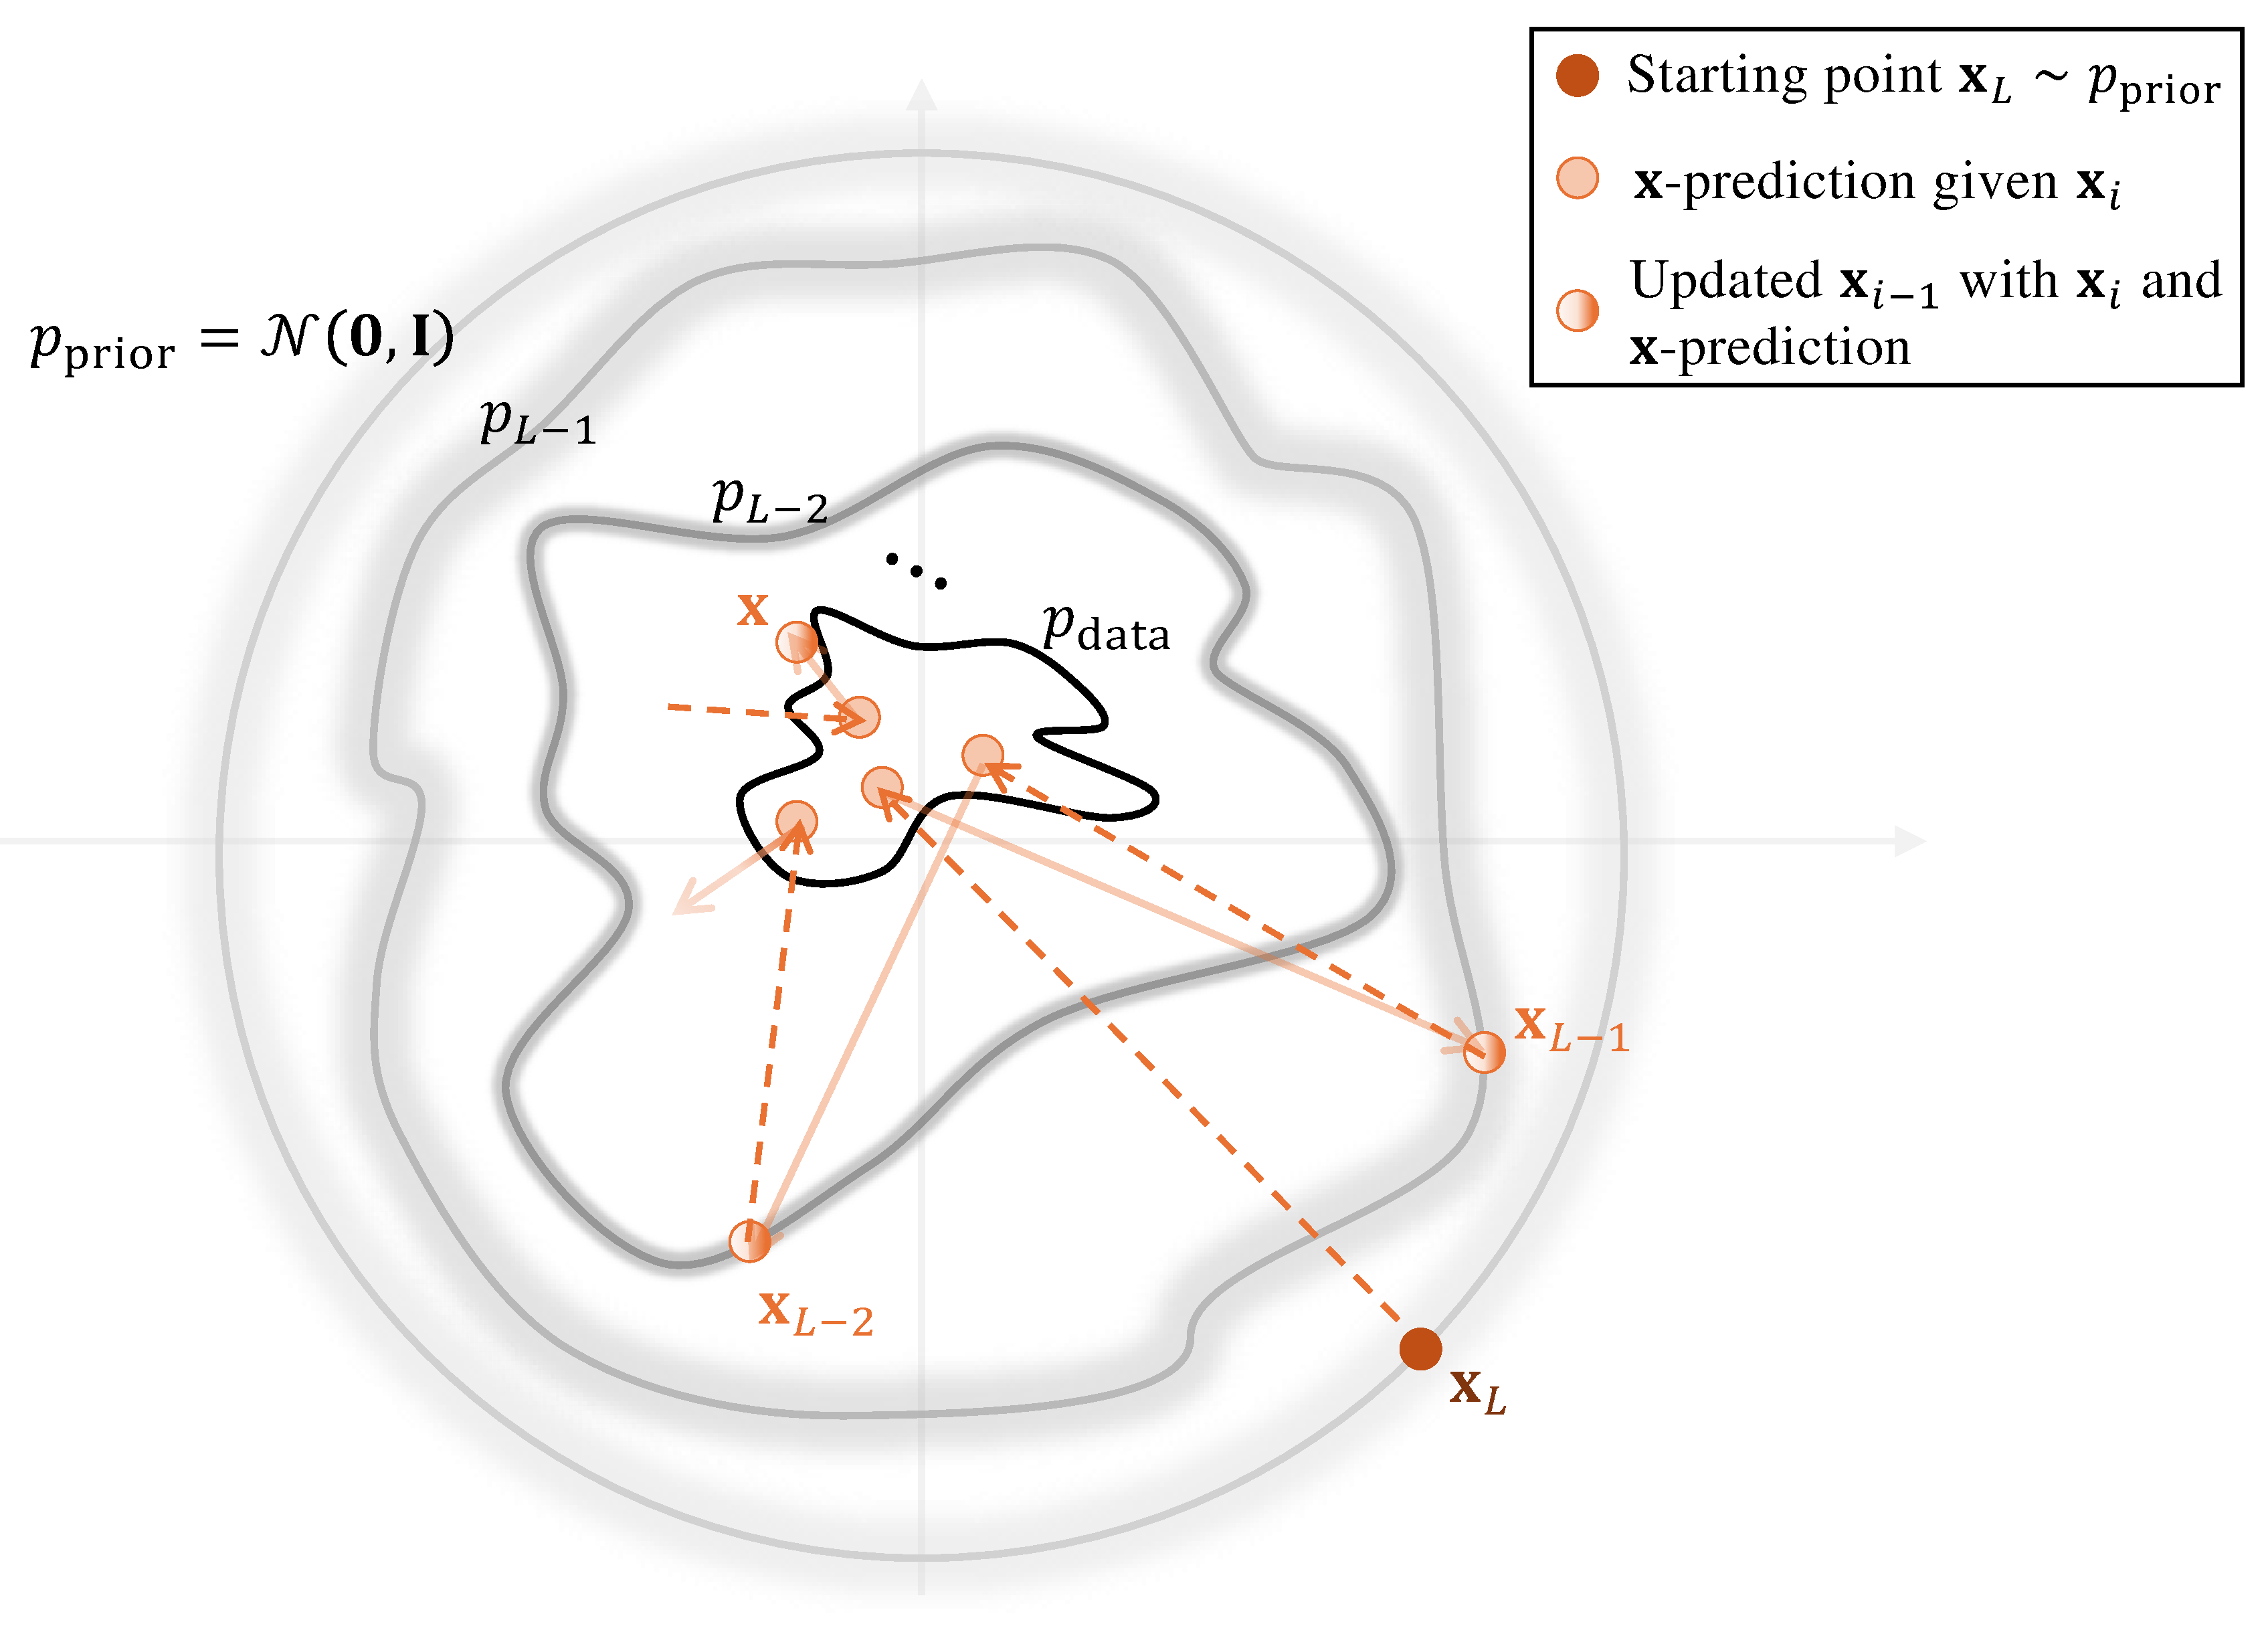
\includegraphics[width=\linewidth]{Images/PartB/diffusion-clean.pdf}
\caption{\textbfs{DDPM 采样“先去噪再重新加噪”视角的示意图。}
从当前噪声样本 $\mathbf{x}_i$ 出发，模型首先估计潜在的干净信号 $\mathbf{x}_{\bm{\phi}^\times}(\mathbf{x}_i,i)$，然后通过将该估计重新加噪至第 $(i-1)$ 个噪声水平来采样一个噪声更小的点 $\mathbf{x}_{i-1}$。\figcredit{由作者绘制。}}
    \label{fig:vdm-clean}
\end{figure}



\paragraph{DDPM 缓慢的采样速度。} DDPM（即扩散模型）的采样本质上是缓慢的。在原始的表述和实现中，生成一个样本通常需要大约 $1{,}000$ 个去噪步骤。这是因为采样通过一长串小的细化进行：在每一步，模型将当前噪声样本稍微向更干净的方向更新，而下一步更新必须从前一步的结果开始。因此，标准 DDPM 采样是时间步进的、强顺序的，而良好的样本质量通常需要许多这样的步骤来紧密跟踪反向扩散路径。

定理~\ref{thm:equiv-marginal-kl} 表明，一个富有表现力的 $ p_{\bm{\phi}}(\mathbf{x}_{i-1} | \mathbf{x}_i) $ 理论上能够匹配真实的反向分布 $ p(\mathbf{x}_{i-1} | \mathbf{x}_i) $。然而在实践中，$ p_{\bm{\phi}}(\mathbf{x}_{i-1} | \mathbf{x}_i) $ 通常被建模为高斯分布以近似 $ p(\mathbf{x}_{i-1} | \mathbf{x}_i) $，这限制了其表达能力。

对于较小的前向噪声尺度 $\beta_i$，真实反向分布近似为高斯分布，从而能够精确近似。相反，较大的 $\beta_i$ 会诱发单高斯无法捕捉的多峰性或强非高斯性。为了保持精度，DDPM 采用许多小的 $\beta_i$ 步骤，形成一条顺序链，其中每一步都依赖于前一步，并需要一次神经网络求值 $\boldsymbol{\epsilon}_{\bm{\phi}^\times}(\mathbf{x}_i, i)$。这导致 $\mathcal{O}(L)$ 次顺序传递，阻碍了并行化并拖慢了生成。



在后面的 \Cref{ch:score-sde} 中，我们将展示对这一固有采样瓶颈的一种更有原则的解释，即将其视为一个微分方程问题，这激发了用于加速生成的连续时间数值策略。



\newpage
\section{结语}\label{sec:ch2_cr}


在本章中，我们通过变分的视角追溯了扩散模型的起源。我们从变分自编码器（VAE）开始，它是一个基础的生成模型，通过证据下界（ELBO）学习数据与一个结构化隐空间之间的概率映射。我们看到层次化 VAE（HVAE）如何通过堆叠隐层来扩展这一思想，引入了渐进式、由粗到细生成的有力概念。然而，这些模型面临训练稳定性和样本质量方面的挑战。





然后，我们将去噪扩散概率模型（DDPM）构建为这一变分框架内的一次关键演进。通过将编码器固定为一个渐进的加噪过程并仅学习反向去噪步骤，DDPM 优雅地避开了 HVAE 的训练不稳定性。关键的是，我们证明了 DDPM 也是通过最大化对数似然上的一个变分界来训练的，其训练目标分解为一系列简单的去噪任务。这种可处理性由一种有力的条件化策略促成，该策略将一个不可处理的边际目标转化为一个可处理的条件目标，这是扩散模型中反复出现的主题。





虽然这一变分框架为 DDPM 提供了一个完整而有力的基础，但它并不是理解它们的唯一方式。一种替代且同样基础的视角从基于能量的建模原理中涌现。在下一章中，我们将探讨这种基于分数的视角：
\begin{enumerate}
    \item 我们将把焦点从学习去噪转移概率 $p_{\bm{\phi}}(\mathbf{x}_{i-1}\vert\mathbf{x}_{i})$ 转移到直接学习数据对数密度的梯度，即分数函数。
    \item 我们将看到这一源于 EBM 的方法如何催生噪声条件分数网络（Noise Conditional Score Network，NCSN），并揭示 DDPM 中学到的噪声预测（$\bm{\epsilon}$-预测）与分数函数本身之间深刻的数学等价性。
\end{enumerate}

这一替代视角不仅将提供新的洞察，还将作为稍后开发的扩散模型统一连续时间框架的另一块基石。








\chapter{分数视角：从 EBM 到 NCSN}\label{ch:score-based}

% In the previous chapters we traced diffusion models back to their variational roots, showing how they emerge from the framework of VAEs. We now turn to a second, equally fundamental view-point: \emph{Energy-Based Models (EBMs)}. EBMs describe data distributions through unnormalized energy functions, and by examining their gradients we arrive at the notion of a \emph{score function}. This chapter builds the bridge from EBMs to what will later crystallize as \emph{score-based diffusion models}. For readers already versed in EBMs, this section serves as a focused refresher and a stepping stone toward the score-based view.

在前几章中，我们将扩散模型追溯到其变分根源，并展示了它们如何在 VAE 的框架内产生。现在我们转向第二个同样基本的视角：\emph{基于能量的模型}（EBM）~\citep{ackley1985learning,lecun2006tutorial}。EBM 通过一个能量景观来表示分布：该景观在数据处能量低，在别处能量高。采样通常依赖于 Langevin 动力学，它通过沿着该景观的梯度移动样本，将其引向高密度区域。这个梯度场被称为\emph{分数}（score），指向概率更高的方向。

核心观察是：仅知道分数就足以进行生成——它能将样本移向高概率区域，而无需计算难以处理的归一化常数。\emph{基于分数的}扩散模型直接建立在这一思想之上。它们不再只关注干净的数据分布，而是考虑一系列被高斯噪声扰动的分布，这些分布的分数更易于近似。学习这些分数得到一族向量场，它们逐步引导带噪样本回归到数据，从而把生成转化为渐进式去噪。




% \se{fix language, ideally give some intuition for this connection}

\newpage


\section{基于能量的模型}\label{sec:ebm}

对于已经熟悉 EBM 的读者，本节作为一个简明的回顾，并作为通向扩散模型分数视角的桥梁。
\subsection{使用能量函数建模概率分布}

设 $\mathbf{x} \in \mathbb{R}^D$ 表示一个数据点。EBM 通过由 ${\bm{\phi}}$ 参数化的能量函数 $E_{\bm{\phi}}(\mathbf{x})$ 定义概率密度，该函数为更可能的配置赋予更低的能量。所得分布为
\begin{align*}
    p_{{\bm{\phi}}}(\mathbf{x}) := \frac{\exp(-E_{\bm{\phi}}(\mathbf{x}))}{Z_\bphi}, \quad 
    Z_\bphi := \int_{\mathbb{R}^D} \exp(-E_{\bm{\phi}}(\mathbf{x})) \diff\mathbf{x},
\end{align*}
其中 $Z_\bphi$ 称为\emph{配分函数}，用于保证归一化：
\[
\int_{\mathbb{R}^D} p_{{\bm{\phi}}}(\mathbf{x})  \diff\mathbf{x} = 1.
\]
\begin{figure}[th!]
    \centering
    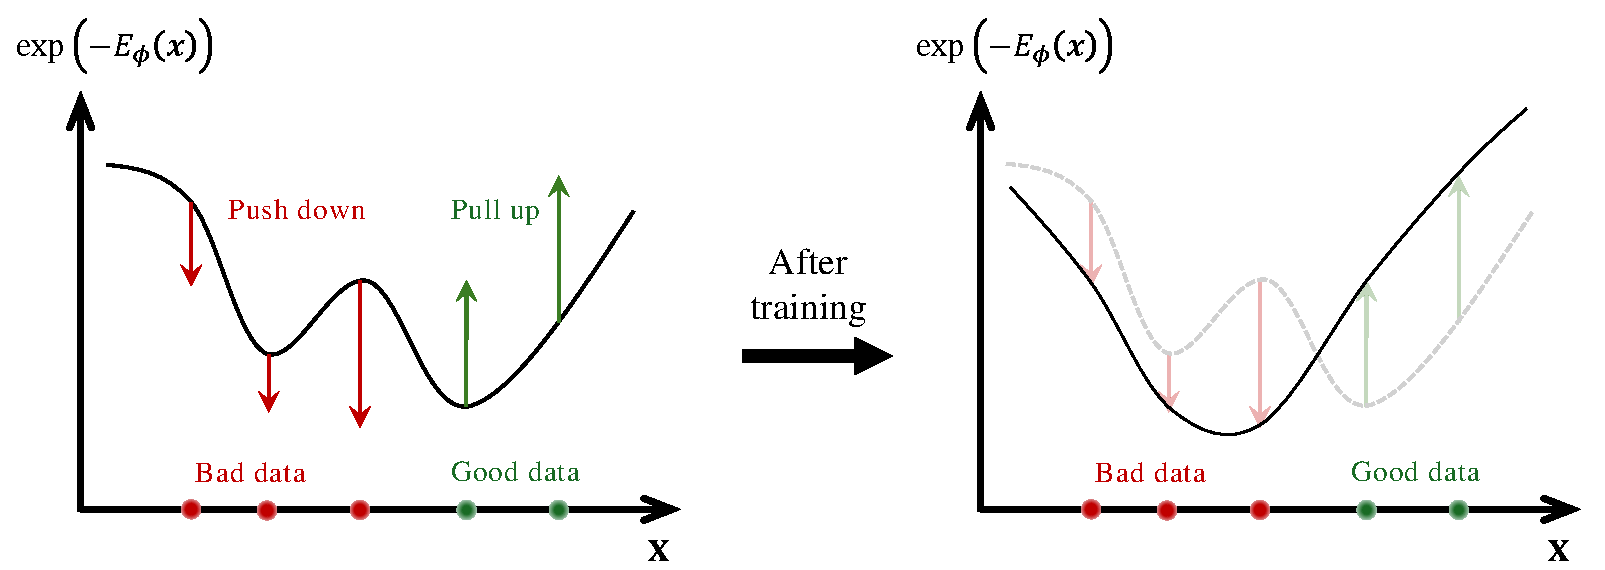
\includegraphics[width=\linewidth]{Images/PartB/ebm-graph.pdf}
    \caption{\textbfs{EBM 训练示意图。} 模型在``坏''数据点处降低密度（升高能量）（红色箭头），并在``好''数据点处升高密度（降低能量）（绿色箭头）。 \figcredit{由作者绘制。}}
    \label{fig:ebm-graph}
\end{figure}



在这种视角下，能量更低的点对应更高的概率，就像一个球滚入山谷一样。配分函数 $Z_{\bphi}$ 确保所有概率之和为一，因此只有能量的\emph{相对}值才起作用。例如，给所有能量加上一个常数会使分子和分母同乘相同的因子，分布保持不变。

此外，由于配分函数 $Z_{\bphi}$ 强制概率之和为一，从数学上可知，降低某一区域内的能量会增加其概率，而其补集的概率则相应减少。因此，EBM 遵循严格的全局权衡：使一个山谷更深必然会使其他山谷变浅，概率质量在整个空间上被重新分配，而非独立地分配给每个区域。


\paragraph{EBM 中极大似然训练的挑战。}
原则上，EBM 可以通过极大似然来训练，这种方法自然地在拟合数据与全局正则化之间取得平衡（见 \Cref{eq:MLE}）：
\begin{align}
\label{eq:mle-ebm}
\mathcal{L}_{\text{MLE}}(\bphi) 
&= \mathbb{E}_{p_{\text{data}}(\rvx)}  \left[ \log \frac{\exp(-E_{\bphi}(\rvx))}{Z_\bphi} \right] \\
&= -  \underbrace{\mathbb{E}_{p_{\text{data}}}[E_{\bphi}(\rvx)]}_{\text{lowers energy of data}}
   -  \underbrace{\log \int \exp(-E_{\bphi}(\rvx))\diff\rvx}_{\text{global regularization}}, \nonumber
\end{align}
其中 $Z_\bphi = \int \exp(-E_\bphi(\rvx))\diff\rvx$。
第一项降低真实数据的能量，而第二项通过配分函数强制归一化。

然而，在高维情形下，计算 $\log Z_{\bphi}$ 及其梯度是难以处理的，因为它需要在模型分布下求期望。
这促使人们寻找替代目标：要么近似该项，例如对比散度\citep{hinton2002training}；要么通过\emph{分数匹配}完全绕开它。

接下来，我们首先在 \Cref{subsec:motivation-score} 中介绍分数函数的概念，并在 \Cref{subsec:training-ebm} 中将分数匹配作为绕开配分函数的可处理训练目标加以介绍，然后在 \Cref{subsec:sampling-ebm} 中讨论将 Langevin 动力学作为一种实用的、基于分数函数的采样方法。

% \paragraph{Preface: Efficient EBM Training via Score Matching.}


% \paragraph{Preface: Sampling via Score Functions.}
% Training alone is not sufficient; EBMs must also generate samples from their learned energy landscape. 
% Since they lack an explicit generator, this is typically achieved with Markov Chain Monte Carlo methods. 
% Among these, \emph{Langevin dynamics} is particularly effective: it updates samples using only the gradient of the energy (the score function), 
% guiding them toward regions of higher probability and enabling efficient sampling without computing the partition function.













% \paragraph{Intuition Behind Energy-Based Models.}
% \jcr{Drawing from the physical analogy of a ball gravitating towards a low-energy valley, Energy-Based Models (EBMs) define a distribution by assigning an \emph{energy} $E_\bphi(\rvx)$ to each point $\rvx$ and converting these values into probabilities $p_\bphi(\rvx) = \tfrac{\exp(-E_\bphi(\rvx))}{Z_\bphi}$. Lower energy means larger $\exp(-E_\bphi(\rvx))$ and thus higher probability mass, so regions where the energy landscape forms deep valleys correspond to more likely and realistic data. The partition function $Z_\bphi$ ensures proper normalization, since $\exp(-E_\bphi(\rvx))$ alone does not integrate to one. Importantly, only relative energies matter: adding a constant $c$ shifts both numerator and denominator by the same factor $e^{-c}$, leaving $p_\bphi$ unchanged.

% This normalization induces a global trade-off across the space. To see this, consider a region $A$, where its probability under $p_\bphi$ is
% \[
% \frac{\int_A \exp(-E_\bphi(\rvx)) \diff\rvx}{\int \exp(-E_\bphi(\rvx)) \diff\rvx} = \frac{\int_A \exp(-E_\bphi(\rvx)) \diff\rvx}{\int \exp(-E_\bphi(\rvx)) \diff\rvx}.
% \]
% If $E_\bphi$ is decreased on $A$, the numerator grows and thus the probability on $A$ increases. Since the denominator grows as well, the relative weight of the complement $A^c$ must shrink so that the total probability remains one. In plain words, making one valley deeper necessarily makes other valleys shallower, because $Z_\bphi$ redistributes probability mass across the entire space. This captures the essence of EBMs: the model does not assign probabilities independently to regions, but balances them through a single global normalization.

% }
% % Drawing from the physical notion that systems gravitate towards lower potential energy (e.g., a ball in a valley), Energy-Based Models define a probability distribution by assigning an \emph{energy} $E_\bphi(\mathbf{x})$ to each data point $\mathbf{x}$. Crucially, lower energy corresponds to higher likelihood and more realistic data, while high energy signals low probability, mirroring how physical systems avoid high-energy configurations. This framework allows EBMs to model intricate, multimodal distributions without explicit latent variables or restrictive parametric assumptions, distinguishing them from approaches like VAEs. 
% % The energy function provides a direct, interpretable measure of data plausibility.
% % \se{won't be clear why without mentioning normalization}

% % \se{need to add citations}



% \paragraph{Challenge of Energy-Based Models.}
% Despite their conceptual appeal, EBMs are challenging to train (and actually also sample) due to the intractability of $Z_\bphi$, which involves integrating over the full input space. Consequently, practical methods rely on approximate or surrogate objectives that bypass direct evaluation of the partition function while still encouraging the model to fit the data distribution.


% \paragraph{Naïve Training of Energy-Based Models.}
% \jc{The fundamental goal when training an EBM is to assign low energy to genuine data points, making them highly probable under our model. In theory, one could drive the energy of training samples arbitrarily low, leading to a degenerate `spiky'' density that places almost all probability on the data and ignores the rest of the space. In practice, however, this collapse is prevented by the smooth and finite capacity parameterization of a neural network $E_\bphi$, which, together with the global normalization constraint, discourages sharply concentrated distributions.
% }
% \se{not sure this overfitting discussion is valuable here}
% This trade-off is naturally captured by the maximum likelihood objective (see \Cref{eq:MLE}), which balances data fitting with global regularization:
% \begin{align}
% \begin{aligned}
%     \label{eq:mle-ebm}
%     \mathcal{L}_{\text{MLE}}({\bm{\phi}}) &= \mathbb{E}_{p_{\text{data}}(\mathbf{x})} \left[ \log \frac{\exp(-E_{\bm{\phi}}(\rvx))}{Z_\bphi} \right] \\
%     &= - \underbrace{\mathbb{E}_{p_{\text{data}}(\mathbf{x})} [E_{\bm{\phi}}(\rvx)]}_{\text{pulls down energy of data}} - \underbrace{\log \int_{\mathbb{R}^D} \exp(-E_{\bm{\phi}}(\mathbf{x})) \diff\mathbf{x}}_{\text{global regularization}},
% \end{aligned}
% \end{align}
% where we use the definition of $Z_\bphi=\int \exp(-E_\bphi(\rvx))\diff\rvx$.
% % \se{probably better to spell out the def of the partition function here (integral) so the tradeoff is clear}
% The first term encourages low energy for real samples, while the second term, via the partition function $Z_\bphi$, penalizes spreading low energy too broadly; thus promoting a well-distributed model.

% % However, computing $Z_\bphi$ is generally intractable, as it involves integrating over the entire data space. Consequently, exact maximum likelihood training is rarely feasible in practice. This motivates the use of approximation methods such as \emph{Contrastive Divergence} or alternative objectives like \emph{Score Matching}, which offer tractable estimates of the gradient. \se{add citations. tie to the divergence discussion in early chapters?}


% \jcr{
% While conceptually simple, evaluating the partition function $Z_\bphi$ is typically intractable because it integrates over the entire space, which makes exact maximum likelihood impractical. Classical approximations such as contrastive divergence~\citep{hinton2002training}, but here we emphasize score matching~\citep{hyvarinen2005estimation}, which replaces likelihood training with the Fisher divergence discussed earlier in \Cref{eq:fisher}. Crucially, this objective avoids $Z_\bphi$ because the score does not depend on the normalization constant. 
% }


% Sampling from EBMs poses another key challenge. Unlike models with explicit decoders, EBMs define only an energy landscape. To generate samples, we typically resort to \emph{Markov Chain Monte Carlo (MCMC)} methods. Unfortunately, many standard MCMC techniques require full likelihood evaluations \se{i don't think that's true, which one are you thinking about?}, which again involve $Z_\bphi$. A widely used workaround is \emph{Langevin Dynamics}, which leverages the gradient of the energy function alone. This allows us to sample effectively from the learned distribution without evaluating the full normalization constant.

% We first discuss in details score matching training technique of EBMs that bypass the need for exact likelihoods, and subsequently move to Langevin Dynamics as a practical sampler.

% \se{this setup training-inference-training is messy}


% \subsection{Motivation--What Is Score?}\label{subsec:motivation-score}

% We begin by formally defining the score function~\citep{stein1972bound}. For a probability density function $ p(\rvx) $ on $ \mathbb{R}^D $, the \emph{score function} is the vector field given by the gradient of the log-density:
% \[
% \rvs(\rvx) := \nabla_{\rvx} \log p(\rvx),
% \]
% where $ \rvs \colon \mathbb{R}^D \to \mathbb{R}^D $.

% The score function can be understood as the gradient field of a probability landscape. Instead of describing absolute likelihoods, it points locally in the direction where probability increases most steeply, thus offering an intuitive and mathematically precise guide for navigating toward regions of higher data density.

% \begin{figure}[th]
%     \centering
%     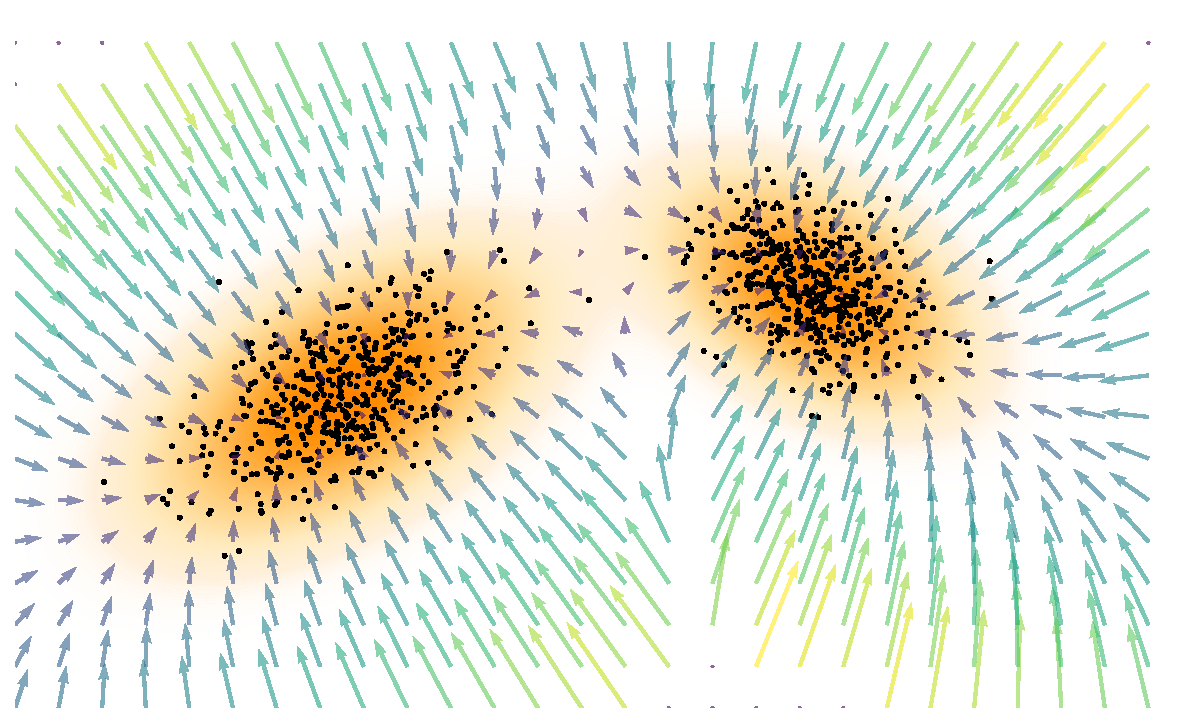
\includegraphics[width=0.95\linewidth]{Images/PartB/score_function_plot.pdf}
%     \caption{Visualization of score vector fields $\nabla_{\rvx} \log p(\rvx)$, which indicate the direction of increasing probability density under $p(\rvx)$.}
%     \label{fig:score-function}
% \end{figure}

% \paragraph{Why the Score Function Excels?}
% \jcr{A natural question arises: why model the score function instead of the probability distribution directly?
% The score provides both theoretical clarity and practical benefits. We start by outlining its conceptual foundations and will highlight further advantages as the chapter unfolds.}
% % One may question the rationale behind modeling the score function rather than the probability distribution itself.
% % \se{fix language. also transition to this paragraph is very rough, this was not mentioned before}
% % Indeed, the score function offers both theoretical and practical advantages. We begin by introducing its conceptual foundations and will progressively highlight additional benefits throughout this chapter.

% \subparagraph{1. Freedom from Normalization Constants.}
% Many distributions are defined only up to an unnormalized density $\tilde{p}(\rvx)$, e.g., $\exp(-E_{\bm{\phi}}(\rvx))$ in EBMs with
% \[
% p(\rvx) = \frac{\tilde{p}(\rvx)}{Z}, 
% \qquad 
% Z = \int \tilde{p}(\rvx)  \diff\rvx.
% \]
% Evaluating $Z_{\bm{\phi}}$ is generally intractable, creating a bottleneck for training.  
% The score function removes this difficulty:
% \begin{align}\label{eq:score-no-constant}
%     \nabla_{\rvx}\log p(\rvx) 
% = \nabla_{\rvx}\log \tilde{p}(\rvx) - \underbrace{\nabla_{\rvx}\log Z}_{=0}
% = \nabla_{\rvx}\log \tilde{p}(\rvx),
% \end{align}
% since $Z$ is constant in $\rvx$.  
% Hence the score depends only on $\tilde{p}$, allowing EBMs to be trained without computing $Z$.



% \subparagraph{2. A Complete and Expressive Representation.}
% Focusing on the score function does not entail any loss of information about the original distribution. The score function uniquely characterizes the distribution since it is the gradient of the log-density. Conversely, the original density can be recovered from the score function up to a constant:
% \[
% \log p(\rvx) = \log p(\rvx_0) + \int_0^1 \rvs(\rvx_0 + t(\rvx - \rvx_0))^\top (\rvx - \rvx_0)  \diff t,
% \]
% where $\rvx_0$ is a reference point and $\log p(\rvx_0)$ acts as an integration constant fixed by normalization. This equivalence establishes that modeling the score function is as expressive as modeling the density itself, offering a tractable alternative for generative modeling.




% \subsection{Training EBMs with Score Matching}\label{subsec:training-ebm}
% % \paragraph{Contrastive Divergence.} 
% % \se{should we cut this? not sure it's relevant}
% % One challenge in training EBMs is the difficulty of sampling from the model. A widely used workaround is \textit{Contrastive Divergence}, which approximates model samples using short-run MCMC.

% % We revisit \Cref{eq:mle-ebm}. Taking the gradient of the MLE objective with respect to $\bm{\phi}$ yields:
% % \begin{align*}
% %     &\nabla_{\bm{\phi}} \mathcal{L}_{\text{MLE}}(\bm{\phi}) \\
% %     =&\mathbb{E}_{p_{\text{data}}(\mathbf{x})} [-\nabla_{\bm{\phi}}E_{\bm{\phi}}(\rvx)] - \mathbb{E}_{p_{{\bm{\phi}}}(\mathbf{x})} [\nabla_{\bm{\phi}}\log Z_\bphi]\\
% %     =&\mathbb{E}_{p_{\text{data}}(\mathbf{x})} [-\nabla_{\bm{\phi}}E_{\bm{\phi}}(\rvx)] - \mathbb{E}_{p_{{\bm{\phi}}}(\mathbf{x})} \left[\frac{1}{Z_\bphi} \int \nabla_{\bm{\phi}} \exp(-E_{\bm{\phi}}(\rvx))    \diff\mathbf{x}\right]\\
% % = &\mathbb{E}_{p_{\text{data}}(\mathbf{x})} \left[ -\nabla_{\bm{\phi}} E_{\bm{\phi}}(\rvx) \right]
% % + \mathbb{E}_{p_{\bm{\phi}}(\mathbf{x})} \left[ \nabla_{\bm{\phi}} E_{\bm{\phi}}(\rvx) \right].
% % \end{align*}
% % This motivates the CD loss:
% % \begin{align}\label{eq:contrastive-div}
% %     \mathcal{L}_{\text{CD}}({\bm{\phi}}) 
% % = \mathbb{E}_{p_{\text{data}}(\mathbf{x})} [E_{\bm{\phi}}(\rvx)] 
% % - \mathbb{E}_{\tilde{p}_{{\bm{\phi}}}(\mathbf{x})} [E_{\bm{\phi}}(\rvx)],
% % \end{align}
% % where $\tilde{p}_{\bm{\phi}}(\mathbf{x})$ is an approximate distribution obtained by running a few MCMC steps (e.g., Langevin dynamics) initialized from a data point. This objective approximates the MLE gradient without requiring full convergence of the Markov chain. However, it still incurs computational cost due to the need to simulate MCMC at each training step.

% Maximum likelihood training of EBMs is difficult because of the partition function. 
% \emph{Score matching}~\citep{hyvarinen2005estimation} provides a practical alternative: rather than fitting normalized probabilities, 
% it aligns the score of the model with those of the data.  
% Since these gradients depend only on the energy function, score matching completely bypasses the partition function as we showed in \Cref{eq:score-no-constant}:
% \jcr{
% \begin{align*}
%     \nabla_{\mathbf{x}} \log p_{\bm{\phi}}(\mathbf{x}) &= \nabla_{\mathbf{x}} \log \frac{\exp(-E_{\bm{\phi}}(\rvx))}{Z_\bphi} \\ &= - \nabla_{\mathbf{x}} E_{\bm{\phi}}(\mathbf{x}) - \underbrace{\nabla_{\mathbf{x}} \log Z_\bphi}_{=0} \\&= - \nabla_{\mathbf{x}} E_{\bm{\phi}}(\mathbf{x}) ,
% \end{align*}
% }
% The score matching objective minimizes the discrepancy between the model's score and the (unknown) data score:
% \begin{align}\label{eq:ebm-sm}
% \mathcal{L}_{\mathrm{SM}}(\bm{\phi}) := \mathbb{E}_{p_{\mathrm{data}}(\mathbf{x})} \left[ \frac{1}{2} \left\| \nabla_{\mathbf{x}} \log p_{\bm{\phi}}(\mathbf{x}) - \nabla_{\mathbf{x}} \log p_{\mathrm{data}}(\mathbf{x}) \right\|_2^2 \right].
% \end{align}
% \paragraph{Score Matching: An Alternative Objective.}
% When the true data score $\nabla_{\mathbf{x}} \log p_{\mathrm{data}}(\mathbf{x})$ is inaccessible, score matching offers an ingenious alternative. Under mild regularity conditions (e.g., vanishing boundary terms), its objective can be elegantly reformulated using integration by parts (see Proposition~\ref{sm-trace}):
% \begin{align*}
% \mathcal{L}_{\mathrm{SM}}(\bm{\phi})
% = \mathbb{E}_{p_{\mathrm{data}}(\mathbf{x})} \left[
% \Tr\left(\nabla_{\mathbf{x}}^2 E_{\bm{\phi}}(\rvx) \right)
% + \frac{1}{2} \left\| \nabla_{\mathbf{x}} E_{\bm{\phi}}(\rvx) \right\|_2^2
% \right] + C,
% \end{align*}
% where $\nabla_{\mathbf{x}}^2 E_{\bm{\phi}}(\rvx)$ denotes the Hessian of $E_{\bm{\phi}}$ with respect to $\mathbf{x}$, and $C$ is a constant independent of $\bm{\phi}$.
% This formulation is particularly appealing because it removes the need to compute the intractable partition function $Z_\bphi$ and avoids costly sampling from the model distribution during training. Nevertheless, score matching introduces its own challenges. Specifically, the requirement to compute second-order derivatives (Hessians) often becomes computationally prohibitive, especially in high-dimensional settings.


\subsection{动机：什么是分数？}\label{subsec:motivation-score}

对于 $\mathbb{R}^D$ 上的密度 $p(\rvx)$，\emph{分数函数}是对数密度的梯度：
\[
\rvs(\rvx) := \nabla_{\rvx} \log p(\rvx), \qquad \rvs \colon \mathbb{R}^D \to \mathbb{R}^D.
\]
直观上，分数构成一个指向更高概率区域的向量场，为数据最可能出现的位置提供局部指引（见 \Cref{fig:score-function}）。

\begin{figure}[th]
    \centering
    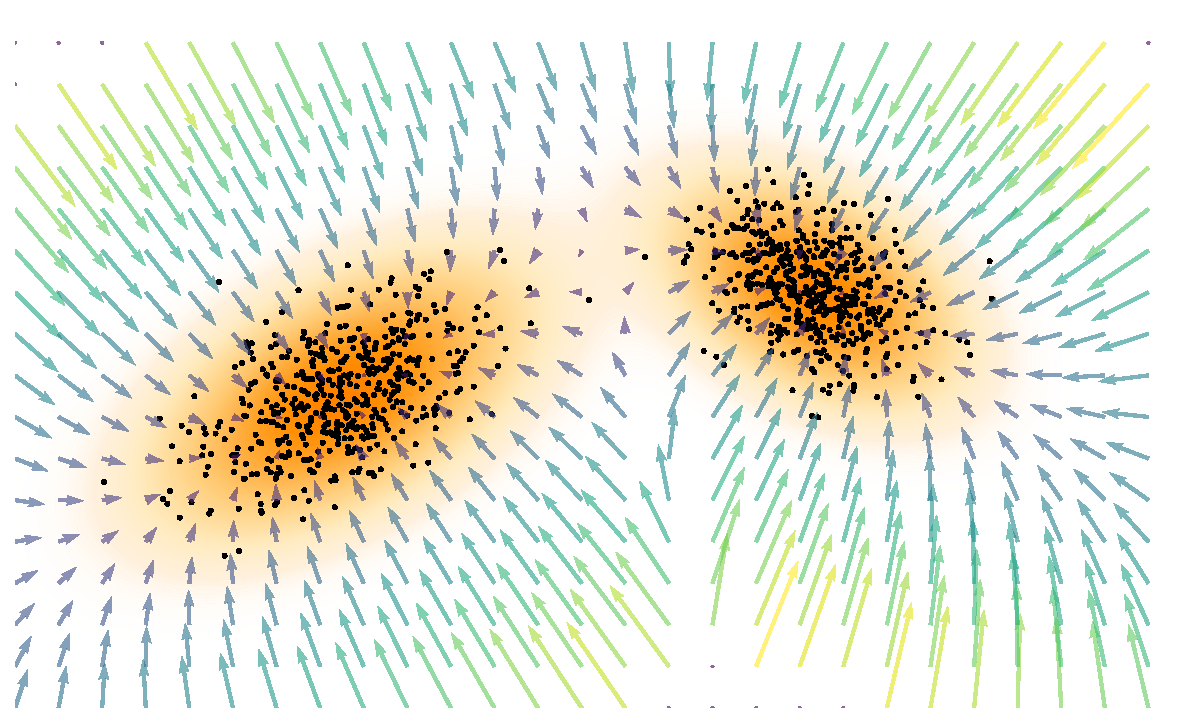
\includegraphics[width=0.95\linewidth]{Images/PartB/score_function_plot.pdf}
    \caption{\textbfs{分数向量场示意图。} 分数向量场 $\nabla_{\rvx} \log p(\rvx)$ 指示密度增加的方向。 \figcredit{由作者绘制。}}
    \label{fig:score-function}
\end{figure}

\paragraph{为什么要建模分数而非密度？}
建模分数在理论和实践上都有优势：


\subparagraph{1. 摆脱归一化常数。}
    许多分布只定义到未归一化密度 $\tilde{p}(\rvx)$，例如 EBM 中的 $\exp(-E_{\bm{\phi}}(\rvx))$：
    \[
    p(\rvx) = \frac{\tilde{p}(\rvx)}{Z}, 
    \qquad 
    Z = \int \tilde{p}(\rvx)\diff\rvx.
    \]
    虽然计算 $Z$ 是难以处理的，但分数只依赖于 $\tilde{p}$：
\begin{align}\label{eq:score-compute}
\nabla_{\rvx}\log p(\rvx) = \nabla_{\rvx}\log \tilde{p}(\rvx) - \underbrace{\nabla_{\rvx}\log Z}_{=0} = \nabla_{\rvx}\log \tilde{p}(\rvx), \end{align} 
因为 $Z$ 关于 $\rvx$ 是常数。这完全绕开了配分函数。

\subparagraph{2. 完整的表示。}
分数函数完整地刻画了底层分布。
由于它是对数密度的梯度，因此密度可以（相差一个常数）通过下式恢复：
\[
\log p(\rvx) 
= \log p(\rvx_0) + \int_0^1 \rvs(\rvx_0 + t(\rvx - \rvx_0))^\top (\rvx - \rvx_0)  \diff t,
\]
其中 $\rvx_0$ 是参考点，$\log p(\rvx_0)$ 由归一化确定。
因此，建模分数与建模 $p(\rvx)$ 本身一样富有表现力，同时在生成建模中往往更易处理。


\subsection{通过分数匹配训练 EBM}\label{subsec:training-ebm}
在 EBM 中，密度定义为 $p_{{\bm{\phi}}}(\mathbf{x}) = \tfrac{\exp(-E_{\bm{\phi}}(\mathbf{x}))}{Z_\bphi}$。极大似然训练需要计算 $Z_{\bm{\phi}}$，而这通常是难以处理的。
一个关键观察是：$p_{{\bm{\phi}}}$ 的模型分数简化为 $-\nabla_{\rvx}E_{\bm{\phi}}(\rvx)$，与 $Z_{\bm{\phi}}$ 无关（见 \Cref{eq:score-compute}）。

\emph{分数匹配}~\citep{hyvarinen2005estimation} 利用了分数只依赖于能量函数这一事实。
它不再拟合归一化概率，而是通过对齐模型分数与（未知的）数据分数来训练 EBM：
\begin{align}\label{eq:ebm-sm}
    \mathcal{L}_{\mathrm{SM}}(\bm{\phi}) 
= \tfrac{1}{2}  \mathbb{E}_{p_{\mathrm{data}}(\mathbf{x})} 
\big\| \nabla_{\mathbf{x}} \log p_{\bm{\phi}}(\mathbf{x}) 
- \nabla_{\mathbf{x}} \log p_{\mathrm{data}}(\mathbf{x}) \big\|_2^2.
\end{align}

尽管数据分数不可得，但分部积分可以得到一个仅涉及能量及其导数的等价表达式（详见命题~\ref{sm-trace}）：
\[
\mathcal{L}_{\mathrm{SM}}(\bm{\phi}) =
\mathbb{E}_{p_{\mathrm{data}}(\mathbf{x})} \left[
-\Tr \big(\nabla_{\mathbf{x}}^2 E_{\bm{\phi}}(\rvx)\big)
+ \tfrac{1}{2}  \|\nabla_{\mathbf{x}} E_{\bm{\phi}}(\rvx)\|_2^2
\right] + C,
\]
其中 $\nabla_{\mathbf{x}}^2 E_{\bm{\phi}}(\rvx)$ 是 $E_{\bm{\phi}}$ 的 Hessian 矩阵，$C$ 是与 $\bm{\phi}$ 无关的常数。

这一表述很有吸引力，因为它消除了配分函数，并避免了在训练过程中从模型中采样。
它的主要缺点是需要二阶导数：尽管只需要 Hessian 矩阵的迹（$\Tr \big(\nabla_{\mathbf{x}}^2 E_{\bm{\phi}}\big)$），而非完整的 Hessian 矩阵，但该项的精确计算通常需要跨输入坐标汇总二阶导数信息，因此其代价通常随输入维度 $D$ 的增加而上升。
我们将在本章后面重新讨论解决该局限的方法。






\subsection{基于分数函数的 Langevin 采样}\label{subsec:sampling-ebm}
从由能量函数 $E_{\bm{\phi}}(\mathbf{x})$ 定义的 EBM 中采样，可以使用\emph{Langevin 动力学}来完成。我们首先介绍离散时间的 Langevin 更新，然后介绍其作为随机微分方程（SDE）的连续时间极限。最后，我们讨论 Langevin 动力学如何实现对复杂能量景观高效探索的物理直觉。


\begin{figure}
    \centering
    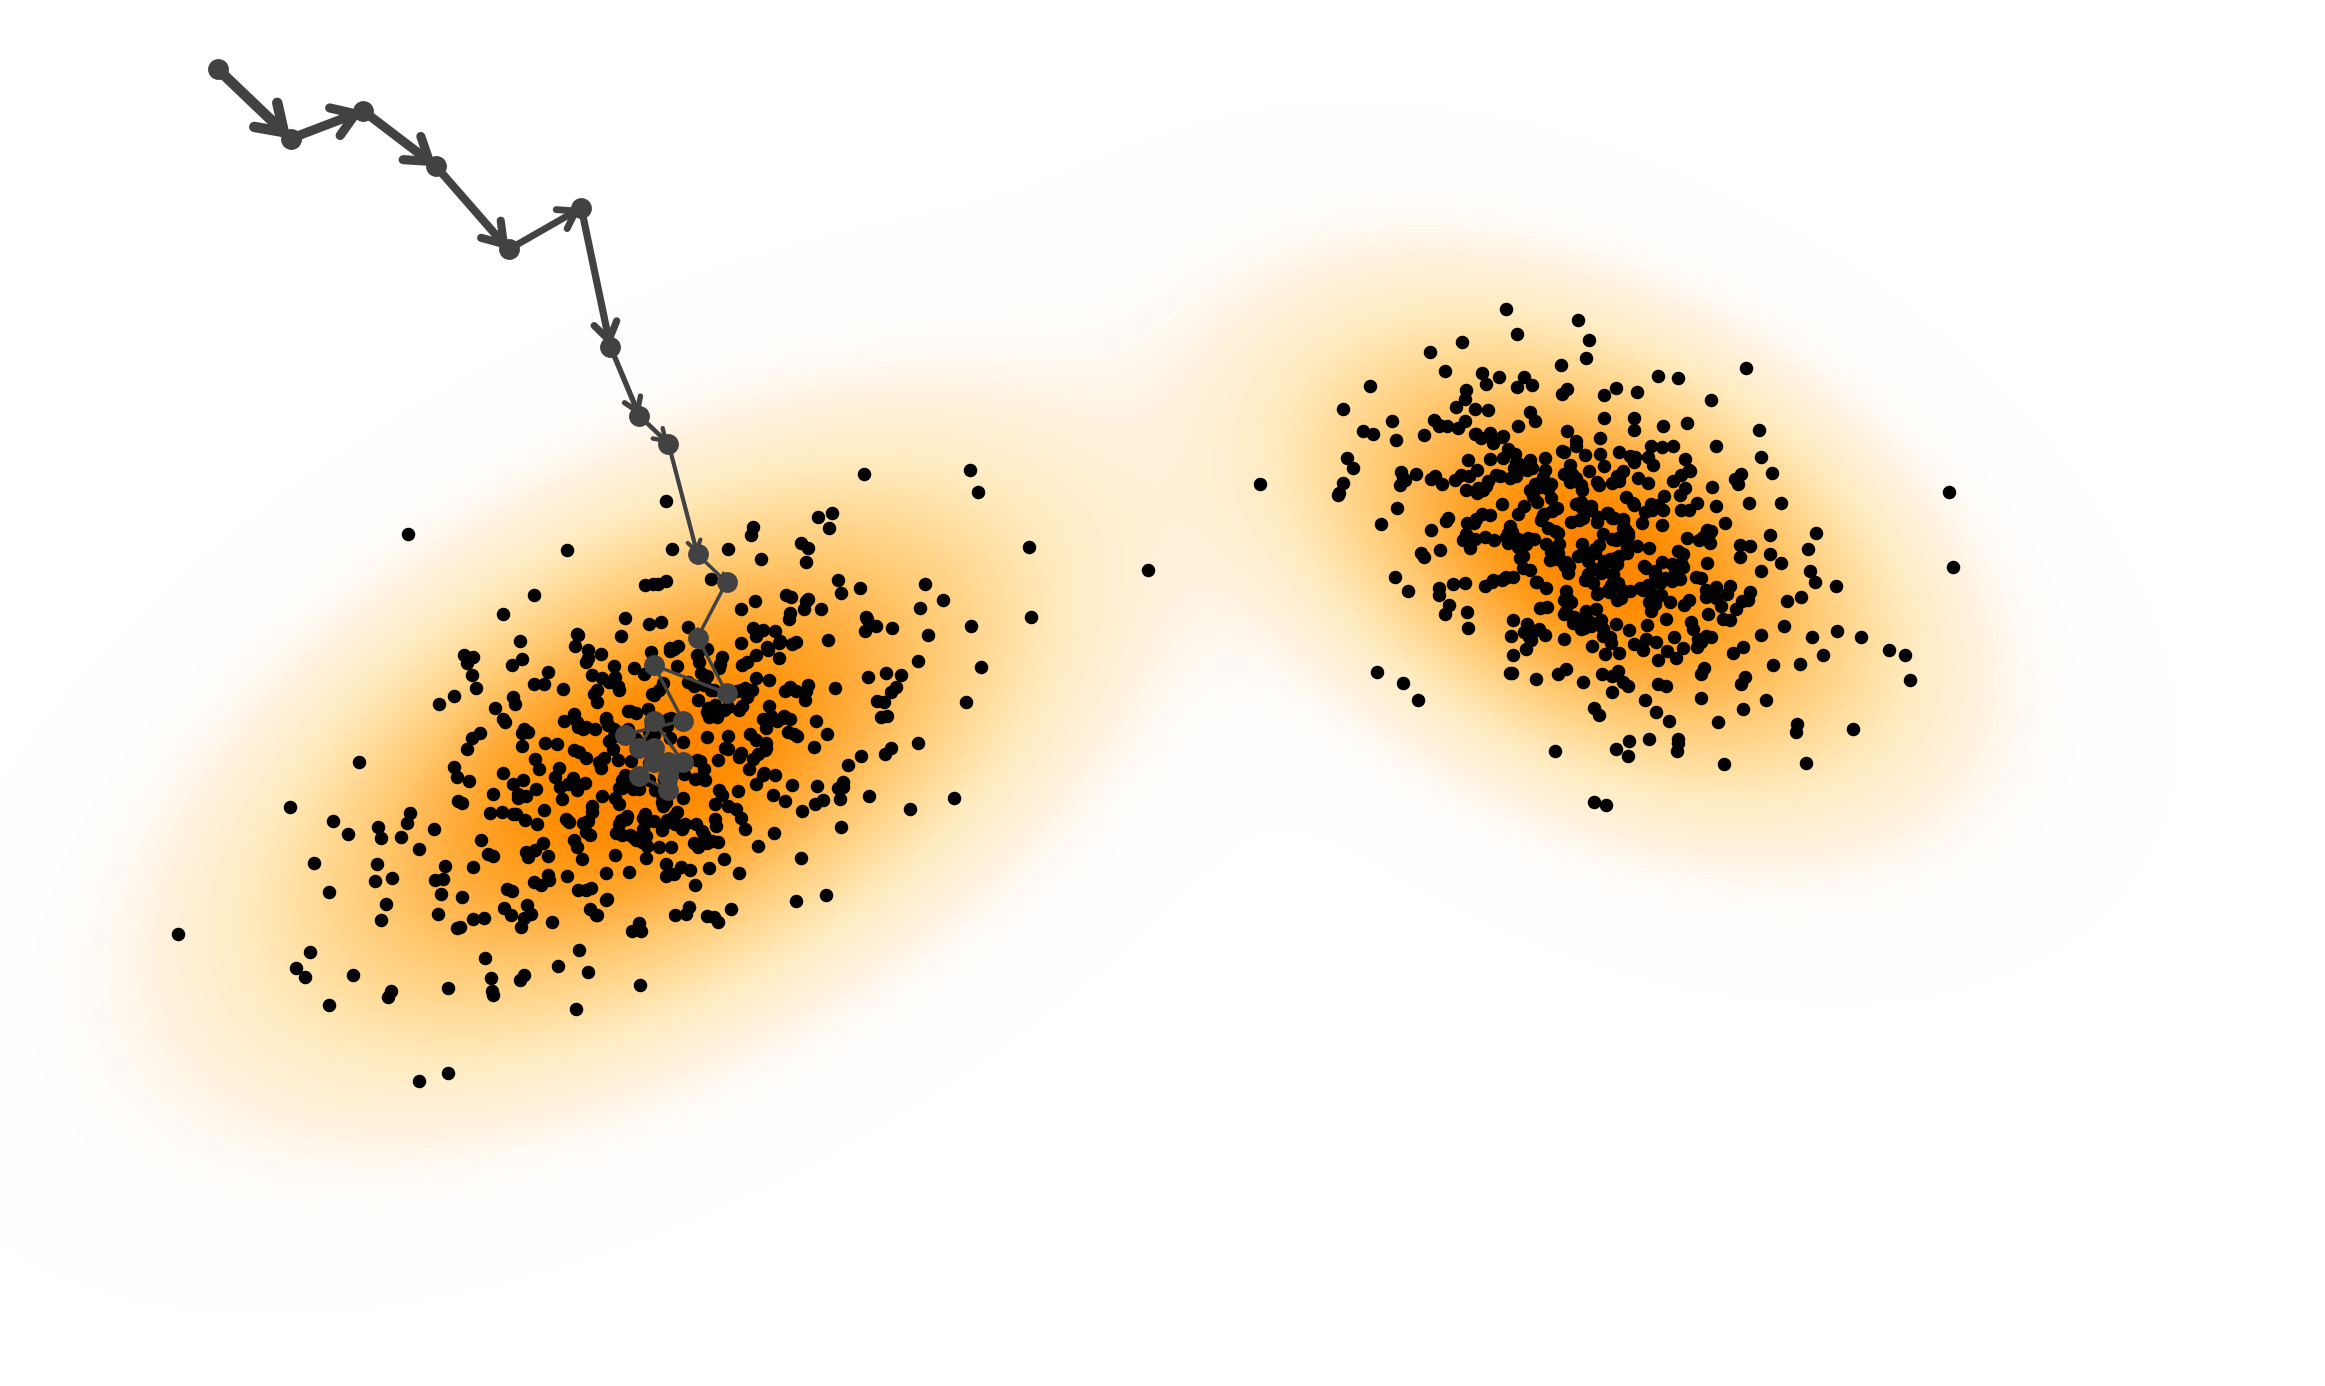
\includegraphics[width=\linewidth]{Images/PartB/langevin_sampling.png}
    \vspace{-1.5cm}
    \caption{\textbfs{Langevin 采样示意图。} Langevin 采样利用分数函数 $\nabla_{\mathbf{x}} \log p_{\bm{\phi}}(\mathbf{x})$，通过 \Cref{eq:discrete-langevin-score} 中的更新（以箭头表示）引导轨迹走向高密度区域。 \figcredit{由作者绘制。}}
    \label{fig:langevin}
\end{figure}


\paragraph{离散时间 Langevin 动力学。}
离散时间的 Langevin 更新为
\begin{align}\label{eq:discrete-langevin}
    \mathbf{x}_{n+1} = \mathbf{x}_n - \eta \nabla_{\mathbf{x}} E_{\bm{\phi}}(\mathbf{x}_n) +  \sqrt{2 \eta} \bm{\epsilon}_n, \quad n=0,1,2,\ldots,
\end{align}
其中 $\mathbf{x}_0$ 由某个分布（通常是高斯分布）初始化，$\eta > 0$ 是步长，$\bm{\epsilon}_n \sim \mathcal{N}(\mathbf{0}, \mathbf{I})$ 是高斯噪声。噪声通过引入随机性使得探索能够超越局部极小值。

由于分数函数可以计算为
\[
\nabla_{\mathbf{x}} \log p_{\bm{\phi}}(\mathbf{x}) = -\nabla_{\mathbf{x}} E_{\bm{\phi}}(\rvx).
\]
% \se{important to show why partition function disappears}
该更新可以等价地写为
\begin{align}\label{eq:discrete-langevin-score}
    \mathbf{x}_{n+1} = \mathbf{x}_n + \eta \nabla_{\mathbf{x}} \log p_{\bm{\phi}}(\mathbf{x}_n) + \sqrt{2 \eta}\bm{\epsilon}_n,
\end{align}
其中分数函数引导样本走向高密度区域。这一表述是扩散模型的核心，后文将详述。

\paragraph{连续时间 Langevin 动力学。}
当步长 $\eta$ 趋近于零时，离散 Langevin 更新自然收敛到一个由\emph{Langevin 随机微分方程（SDE）}描述的连续时间过程\footnote{
带有因子 $\sqrt{2}$ 时，Langevin 动力学使 $p_{\bm\phi}$ 不随时间变化。即 $p_{\bm\phi}$ 是平稳的：若 $\rvx(0)\sim p_{\bm\phi}$，则对所有 $t\ge 0$ 都有 $\rvx(t)\sim p_{\bm\phi}$。等价地，$p_{\bm\phi}$ 是 Fokker–Planck 方程的平稳解（见 \Cref{app:continuity}）：
\[
\partial_t \rho = -\nabla \cdot(\rho  \nabla\log p_{\bm\phi}) + \tfrac{\sigma^2}{2}\Delta \rho.
\]
令 $\rho=p_{\bm\phi}$ 得到 $(\tfrac{\sigma^2}{2}-1)\Delta p_{\bm\phi}=0$，仅当 $\sigma=\sqrt{2}$ 时成立。
}
：
\begin{align}\label{eq:continuous-langevin}
 \diff \mathbf{x}(t) = \nabla_{\mathbf{x}} \log p_{\bm{\phi}}(\mathbf{x}(t)) \diff t + \sqrt{2} \diff \mathbf{w}(t),
\end{align}
其中 $\mathbf{w}(t)$ 表示标准布朗运动（也称为 Wiener 过程\footnote{布朗增量满足
$\mathbf{w}(t+\eta)-\mathbf{w}(t)\sim \mathcal{N}(\mathbf{0},  \eta  \mathbf{I})$。
因此 Euler–Maruyama 使用步噪声 $\sqrt{2}  [\mathbf{w}(t+\eta)-\mathbf{w}(t)]
= \sqrt{2\eta}  \bm{\epsilon}_n$，其中 $\bm{\epsilon}_n \sim \mathcal{N}(\mathbf{0},\mathbf{I})$，
这解释了 $\sqrt{\eta}$ 因子；这就是平方根缩放的来源。关于布朗运动和 SDE 的详细介绍，请参阅 \Cref{app:de}.})。需要理解的是，\Cref{eq:discrete-langevin} 中的离散更新规则是这一连续 SDE 的 Euler–Maruyama 离散化。
% \se{will people be confused by the square root on the step size?}


在标准的正则性假设下（例如 $p_{\bm{\phi}}\propto e^{-E_{\bm{\phi}}}$，且 $E_{\bm{\phi}}$ 具有约束性、足够光滑），$\mathbf{x}(t)$ 的分布随 $t\to\infty$（指数级快速）收敛到 $p_{\bm{\phi}}$；因此我们可以通过模拟（求解）SDE \Cref{eq:continuous-langevin} 来采样。



\paragraph{为什么使用 Langevin 采样？}
理解 Langevin 采样的一种自然方式是从物理学视角：能量函数 $ E_{\bm{\phi}}(\mathbf{x}) $ 定义了一个塑造粒子行为的势能景观。根据牛顿动力学，粒子在该能量所导出的力场下的运动由常微分方程（ODE）描述
\[
\diff \mathbf{x}(t) = -\nabla_{\mathbf{x}} E_{\bm{\phi}}\big(\mathbf{x}(t)\big)  \diff t,
\]
它确定性地将粒子沿势能下降方向推向能量函数的局部极小值。然而，这种确定性动力学可能被困在局部极小值中，从而阻碍对完整数据分布的探索。

为克服这一局限，Langevin 动力学引入随机扰动，得到如下 SDE
\[
\diff \mathbf{x}(t) = -\nabla_{\mathbf{x}} E_{\bm{\phi}}\big(\mathbf{x}(t)\big)  \diff t + \underbrace{\sqrt{2 } \diff \rvw(t)}_{\text{injected noise}},
\]
其中 $\rvw(t)$ 是标准布朗运动。
% and $\eta > 0$ is the diffusion coefficient controlling the noise intensity. \se{no diffusion coeff in equation}
噪声项使粒子能够通过越过能量势垒逃出局部极小值，使轨迹成为一个平稳分布收敛到 Boltzmann 分布的随机过程
\[
p_{\bm{\phi}}(\mathbf{x}) \propto e^{-E_{\bm{\phi}}(\mathbf{x})}.
\]

从这个角度看，EBM 可以被视为学习一个力场，它将样本推向高概率区域。Langevin 采样对 EBM 尤为有用，因为它提供了一种实用的方法，能在不显式计算配分函数的情况下从模型分布 $p_{\bm{\phi}}(\mathbf{x})$ 中生成样本。通过迭代地应用 Langevin 更新，可以得到近似目标分布的样本。


\paragraph{Langevin 采样的固有挑战。}
Langevin 动力学作为一种广泛使用的基于马尔可夫链蒙特卡洛（MCMC）的采样器，在高维空间中面临严重局限。其效率对步长 $\eta$、噪声尺度的选择，以及准确近似目标分布所需的迭代次数高度敏感。

这种低效的核心在于``混合时间''过长的问题：在具有许多孤立模态的复杂数据分布中，Langevin 采样通常需要极长时间才能在高概率区域之间转移。这一问题随维度增加而显著恶化，导致收敛速度慢得令人难以承受。

可以把采样想象成在一片广袤崎岖、有许多遥远山谷（每个山谷对应一个不同的数据模态）的景观中探索。Langevin 动力学依赖局部随机更新，难以高效地在这些山谷之间穿行。因此，它往往无法捕捉分布的全部多样性。

这种低效暗示了我们需要更具结构性和引导性的采样方法，以比纯随机探索更有效地在复杂数据流形上游走。



% Secondly, and also fundamentally, score matching primarily constrains the energy function only at the (local) training data points. It fails to impose explicit global regularization on the overall energy landscape, leaving energy values in regions far from training data loosely controlled. This can lead to undesirable or unconstrained model behavior, a crucial difference from directly modeling probability densities. The latter inherently regularizes the entire distribution by implicitly enforcing a global ``sum-to-one'' rule on probabilities, ensuring more stable energy values across the data space.
% \subsection{Closing Remark}
% EBMs and score matching are closely connected. While much research has focused on improving the efficiency and scalability of score matching for training EBMs~\citep{vincent2011connection,song2020sliced}, its role has significantly evolved. Originally developed as an elegant solution to the intractable normalization constant in unnormalized statistical models such as EBMs, score matching has since become a fundamental building block of modern diffusion models. We will explore this important connection in greater detail in the following sections.






\clearpage
\newpage

% \se{the structure of this chapter is unecessarily convoluted. the story is going to be cleaner if you don't mark the background as optional (anyways it's short) and have a coherent story where you have representation, learning, inference. right now therre is too much back and forth between scores, sampling, score matching}


% Consider a landscape representing the probability distribution over data points, where regions of higher elevation correspond to higher likelihoods, and lower regions correspond to lower likelihoods. At each point in this landscape, imagine an arrow indicating the direction of steepest ascent, guiding movement toward areas of increasing probability. This vector field is known as the \emph{score function}~\citep{stein1972bound}, providing an intuitive and precise direction for navigating the probability landscape.


% \subsection{Motivation--What Is Score?}
% We begin by formally defining the score function. For a probability density function $ p(\rvx) $ on $ \mathbb{R}^D $, the \emph{score function} is the vector field given by the gradient of the log-density:
% \[
% \rvs(\rvx) := \nabla_{\rvx} \log p(\rvx),
% \]
% where $ \rvs \colon \mathbb{R}^D \to \mathbb{R}^D $.

% \begin{figure}[th]
%     \centering
%     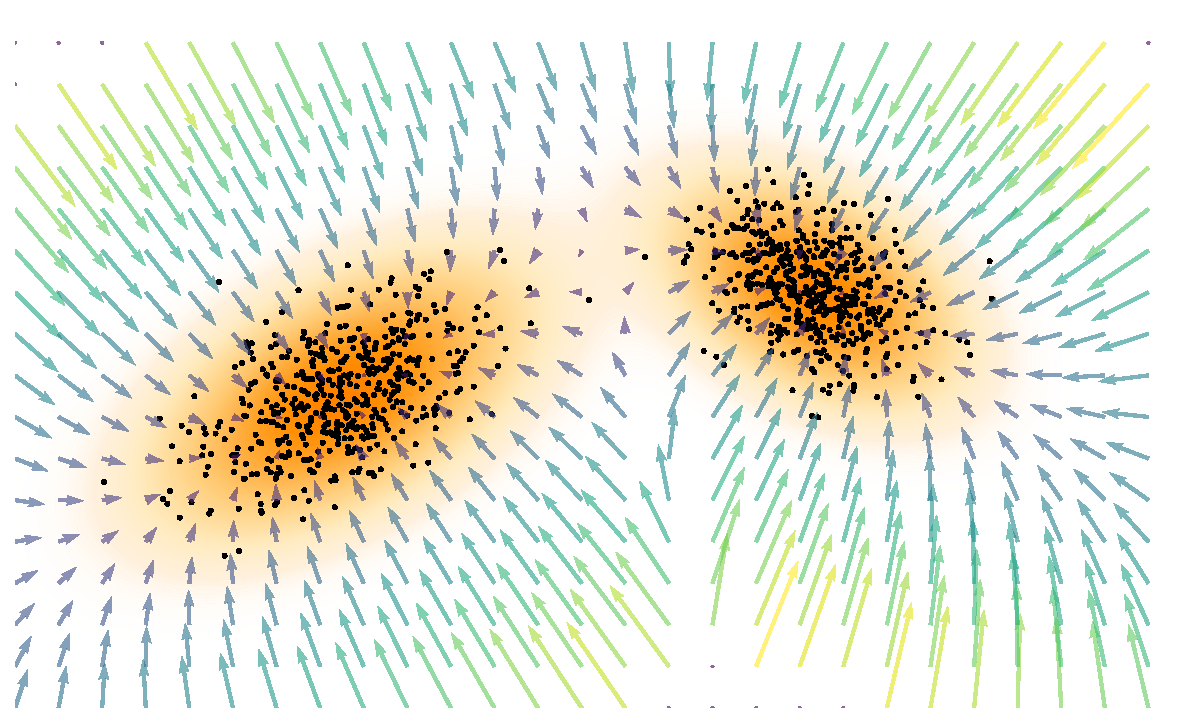
\includegraphics[width=0.95\linewidth]{Images/PartB/score_function_plot.pdf}
%     \caption{Visualization of score vector fields $\nabla_{\rvx} \log p(\rvx)$, which indicate the direction of increasing probability density under $p(\rvx)$.}
%     \label{fig:score-function}
% \end{figure}

% \paragraph{Why the Score Function Excels?}
% One may question the rationale behind modeling the score function rather than the probability distribution itself.
% \se{fix language. also transition to this paragraph is very rough, this was not mentioned before}
% Indeed, the score function offers both theoretical and practical advantages. We begin by introducing its conceptual foundations and will progressively highlight additional benefits throughout this chapter.

% \subparagraph{1. Freedom from Normalization Constants.}
% Many probability distributions are initially defined by an unnormalized density $\tilde{p}(\rvx)$. To turn this into a true probability density $ p(\rvx) $, we must divide by a normalization constant $Z = \int \tilde{p}(\rvx)    \diff \rvx$. Calculating this $Z$ is often computationally prohibitive, involving intractable integrals. This difficulty is a significant bottleneck in training many models, such as EBMs.

% The score function, however, elegantly bypasses this challenge. Consider the derivative:
% \[
% \nabla_{\rvx} \log p(\rvx) = \nabla_{\rvx} \log \left( \frac{\tilde{p}(\rvx)}{Z} \right) = \nabla_{\rvx} \log \tilde{p}(\rvx) - \underbrace{\nabla_{\rvx} \log Z}_{=0}.
% \]
% Since $Z$ is a constant with respect to $ \rvx $, its gradient is zero.
% \[
% \nabla_{\rvx} \log p(\rvx) = \nabla_{\rvx} \log \tilde{p}(\rvx).
% \]
% This remarkable property means the score function is entirely independent of the normalization constant. We can operate directly with unnormalized densities, freeing us from the immense computational burden of computing or approximating $Z$.

% \subparagraph{2. A Complete and Expressive Representation.}
% Focusing on the score function does not entail any loss of information about the original distribution. The score function uniquely characterizes the distribution since it is the gradient of the log-density. Conversely, the original density can be recovered from the score function up to a constant:
% \[
% \log p(\rvx) = \log p(\rvx_0) + \int_0^1 \rvs(\rvx_0 + t(\rvx - \rvx_0))^\top (\rvx - \rvx_0)  \diff t,
% \]
% where $\rvx_0$ is a reference point and $\log p(\rvx_0)$ acts as an integration constant fixed by normalization. This equivalence establishes that modeling the score function is as expressive as modeling the density itself, offering a tractable alternative for generative modeling.



% \paragraph{Using the Score for Generation.}
% Having established that the score function  is a complete and unburdened representation of a distribution, a pivotal question arises:
% \begin{question}
%     Can we actually generate new samples from a complex data distribution if we only know its score function, $ \rvs(\cdot) = \nabla_{\rvx} \log p_{\mathrm{data}}(\cdot) $?
% \end{question}
% The answer is affirmative, owing to a powerful iterative procedure,  \emph{Langevin dynamics}, as introduced in \Cref{eq:discrete-langevin-score}:
% \begin{align}\label{eq:score-langevin}
%     \rvx_{n+1} = \rvx_n + \eta \rvs(\rvx_n) + \sqrt{2\eta} \bm{\epsilon}_n, \quad n=0,1,2,\dots,
% \end{align}
% The process begins from an arbitrary initial point $\rvx_0$ with a step size $\eta > 0$. At each iteration, the sample is nudged in the direction of the score,  ascending the probability landscape; while random noise encourages exploration. Under suitable conditions, \se{need to cite and probably say what the conditions are for completeness} this simple yet powerful procedure produces samples from $p_{\mathrm{data}}$. This demonstrates a key strength of score-based modeling: generating realistic data requires only the score function, not the full probability density.

\section{\texorpdfstring{从基于能量到基于分数的生成模型}{从基于能量到基于分数的生成模型}}
EBM 表明，生成只依赖于分数（它指向更高概率的区域），而不依赖于完整的归一化密度。
虽然分数匹配避开了配分函数，但通过能量进行训练仍然需要昂贵的二阶导数。
关键思想是：既然用 Langevin 动力学采样只需要分数，我们就可以直接用神经网络来学习它。
这种从建模能量到建模分数的转变，构成了基于分数的生成模型的基础.






\begin{figure}[ht!]
    \centering
    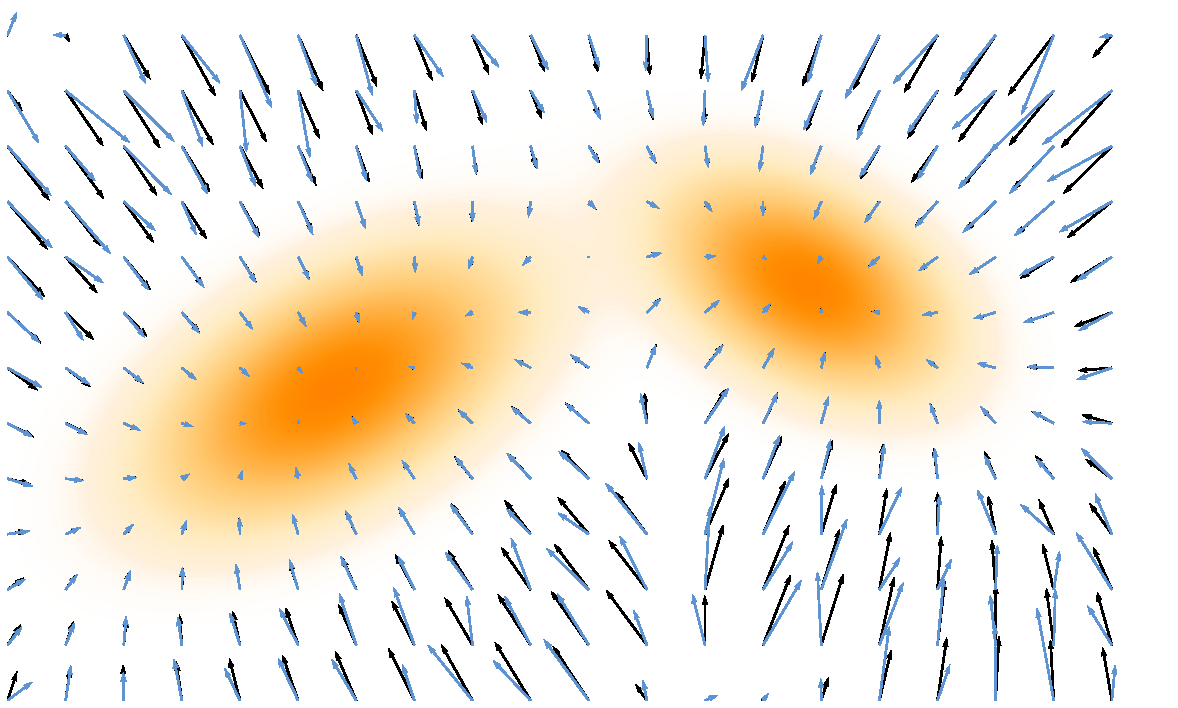
\includegraphics[width=0.9\linewidth]{Images/PartB/score_function_approximation.pdf}
    \caption{\textbfs{分数匹配示意图。} 神经网络分数 ${\color{customblue}\rvs_{\bm{\phi}}(\rvx)}$ 通过 MSE 损失训练以匹配真实分数 $\rvs(\rvx)$。两者都表示为向量场。 \figcredit{由作者绘制。}}
    \label{fig:sm-illustration}
\end{figure}

\subsection{通过分数匹配进行训练}\label{subsec:training-sm}
\paragraph{分数匹配。}
为了从 $p_{\mathrm{data}}$ 的样本中近似分数函数 $\rvs(\rvx) = \nabla_{\rvx} \log p_{\mathrm{data}}(\rvx)$，
我们将其直接近似为由神经网络 $\rvs_{\bm{\phi}}(\rvx)$ 参数化的向量场（见 \Cref{fig:sm-illustration}）：
\[
\rvs_{\bm{\phi}}(\rvx) \approx \rvs(\rvx).
\]
\emph{分数匹配}通过最小化真实分数与估计分数之间的均方误差（MSE）来拟合该向量场：
\begin{mdframed}
\begin{align}\label{eq:sm}
    \mathcal{L}_{\mathrm{SM}}(\bm{\phi}) 
    := \frac{1}{2}  \mathbb{E}_{\rvx \sim p_{\mathrm{data}}}
    \Big[\| \rvs_{\bm{\phi}}(\rvx) - \rvs(\rvx)\|_2^2\Big].
\end{align}
\end{mdframed}

\paragraph{可处理的分数匹配。}
乍看之下，这个目标似乎不可行，因为作为回归目标的真实分数 $\rvs(\rvx)$ 是未知的。
幸运的是，\citet{hyvarinen2005estimation} 证明了分部积分可以得到一个等价目标，它只依赖于模型 $\rvs_{\bm{\phi}}$ 和数据样本，而无需访问真实分数。
我们在下面的命题中陈述这一关键结果：
\proppp{Hyvärinen 的 SM 可处理形式}{sm-trace}
        {
        我们可以将下式表示为：
        \begin{align*}
            \mathcal{L}_{\text{SM}}(\bm{\phi}) = \widetilde{\mathcal{L}}_{\text{SM}}(\bm{\phi}) + C.
        \end{align*}
        其中
        \begin{align}\label{eq:sm-alternative}
            \widetilde{\mathcal{L}}_{\text{SM}}(\bm{\phi})
            := \mathbb{E}_{\rvx \sim p_{\text{data}}(\rvx)} \left[
            \Tr\left(\nabla_{\rvx}\rvs_{\bm{\phi}}(\rvx)\right)
            + \frac{1}{2} \norm{\rvs_{\bm{\phi}}(\rvx)}_2^2
            \right].
        \end{align}
        且 $C$ 是不依赖于 $\bm{\phi}$ 的常数。最小化解 $\rvs^*$ 为：$\rvs^*(\cdot) = \nabla_{\rvx} \log p(\cdot)$。
        }
        {该结果通过展开 $ \mathcal{L}_{\text{SM}} $ 中的 MSE 并应用分部积分得到。证明见 \Cref{app-sec:sm-trace}。
        }

利用 \Cref{eq:sm-alternative} 中的等价目标，我们仅从 $p_{\mathrm{data}}$ 的观测样本训练分数模型 $\rvs_{\bm{\phi}}(\rvx)$，消除了对真实分数函数的需求。


\paragraph{\Cref{eq:sm-alternative} 的直觉。}
替代的分数匹配目标 $\widetilde{\mathcal{L}}_{\text{SM}}(\bm\phi)$
可以直接从它的两项来理解。
范数项 $\tfrac12\|\rvs_{\bm\phi}(\rvx)\|^2$ 在
$p_{\mathrm{data}}$ 较大的区域抑制分数，使这些区域成为驻点。
散度项 $\Tr(\nabla_{\rvx} \rvs_{\bm\phi}(\rvx))$ 在损失中以正号出现，因此最小化该目标会偏好该项取负值。
于是，这些驻点倾向于作为吸引性的汇。
综合来看，该损失将高密度区域塑造成分数场中稳定且收缩的点。
我们在下面详细解释这一点。

\subparagraph{由幅值项得到的驻点性。}
由于 $\widetilde{\mathcal{L}}_{\mathrm{SM}}(\bm\phi)$ 中的期望是在
$p_{\mathrm{data}}$ 下取的，$p_{\mathrm{data}}(\rvx)$ 较大的区域（高数据密度）
对损失的贡献最大。因此幅值项
$\tfrac12\|\rvs_{\bm\phi}(\rvx)\|^2$ 恰恰在这些高概率区域驱动
$\rvs_{\bm\phi}(\rvx)\to 0$，即这些位置变为\emph{驻点}。

\subparagraph{当向量场（近似）为梯度时的凹性。}
由于散度项 $\Tr(\nabla_{\rvx} \rvs_{\bm\phi}(\rvx))$ 以正号进入损失，最小化该目标会促使向量场在高数据密度区域具有负散度。负散度意味着邻近向量会收敛而非散开，因此该区域中的驻点充当\emph{汇}：附近的轨迹被向内牵引。为精确说明这一点，假设
$\rvs_{\bm\phi}=\nabla_{\rvx}u$（其中 $u:\R^D\to\R$ 为标量函数），这在匹配对数密度时是自然的。于是 $\nabla_{\rvx}\rvs_{\bm\phi}=\nabla_{\rvx}^2 u$（Hessian 矩阵）且
$\nabla \cdot \rvs_{\bm\phi}(\rvx)=\Tr(\nabla_{\rvx}^2 u(\rvx))$（散度）。

在驻点 $\rvx_\star$ 处（其中 $\rvs_{\bm\phi}(\rvx_\star)=\nabla_{\rvx}u(\rvx_\star)=\mathbf{0}$），
二阶泰勒展开给出
\[
u(\rvx)
= u(\rvx_\star)
+ \tfrac12(\rvx-\rvx_\star)^\top \nabla_{\rvx}^2 u(\rvx_\star)(\rvx-\rvx_\star)
+ o(\|\rvx-\rvx_\star\|^2).
\]
若 Hessian 矩阵 $\nabla_{\rvx}^2 u(\rvx_\star)$ 负定，则 $u$ 在
$\rvx_\star$ 处局部凹，且对数密度在该处取得严格局部极大值\footnote{我们指出，严格凹性（从而对数密度的严格局部极大值）要求整个 Hessian 矩阵
$\nabla_{\rvx}^2 u$ 负定，而不仅仅迹为负。
负的迹保证了特征值之和为负，但某些特征值仍可能
为正，从而得到鞍点而非极大值。
}。
由于 Hessian 矩阵的所有特征值都为负，迹也为负：
$\Tr(\nabla_{\rvx}^2 u(\rvx_\star))<0$。
因此所学到的向量场具有负散度，该驻点是一个\emph{汇}：微小扰动会被收缩回 $\rvx_\star$。




\subsection{用 Langevin 动力学采样}
一旦通过最小化 \Cref{eq:sm-alternative} 完成训练，分数模型 $\rvs_{\bm{\phi}^\times}(\rvx)$ 就可以在 Langevin 动力学中替代神谕分数进行采样：
\begin{align}\label{eq:score-langevin-emp}
    \mathbf{x}_{n+1} = \mathbf{x}_n + \eta   \rvs_{\bm{\phi}^\times}(\rvx_n) + \sqrt{2\eta}    \bm{\epsilon}_n, \quad \bm{\epsilon}_n \sim \mathcal{N}(\bm{0}, \bm{I}),
\end{align}
其中 $n=0,1,2,\dots$，并以 $\rvx_0$ 初始化。与 EBM 情形 \Cref{eq:continuous-langevin} 一样，该递推恰好是连续时间 Langevin SDE 的 Euler–Maruyama 离散化：
\begin{align*}
    \diff \rvx(t) = \rvs_{\bm{\phi}^\times}(\rvx(t)) \diff t + \sqrt{2} \diff \mathbf{w}(t),
\end{align*}
初始化为 $\rvx(0)$。因此，在小步长极限下，离散与连续表述一致。在实践中，既可以运行离散采样器，也可以直接模拟 SDE。



\subsection{序章：基于分数的生成模型}

在本章余下部分，我们考察分数函数在现代扩散模型中的基础性作用。分数函数最初被引入是为了实现 EBM 的高效训练，如今已演变为新一代生成模型的核心组件。在此基础上，我们探讨分数函数如何为\emph{基于分数的扩散模型}的理论形式和实际实现提供依据，从而为通过随机过程进行数据生成提供一个有原则的框架。


\clearpage
\newpage


\section{\texorpdfstring{去噪分数匹配}{去噪分数匹配}}\label{sec:dsm}

\subsection{动机}
尽管 \Cref{eq:sm-alternative} 中的替代目标
\begin{align*}
    \widetilde{\mathcal{L}}_{\text{SM}}(\bm{\phi}) = \mathbb{E}_{\rvx \sim p_{\mathrm{data}}} \left[\mathrm{Tr}\big(\nabla_{\rvx}\rvs_{\bm{\phi}}(\rvx)\big) + \frac{1}{2} \|\rvs_{\bm{\phi}}(\rvx)\|_2^2 \right]
\end{align*}
更易处理，但它仍然需要计算 Jacobi 矩阵的迹 $\mathrm{Tr}(\nabla_{\rvx}\rvs_{\bm{\phi}}(\rvx))$。虽然这不需要构造完整的 Jacobi 矩阵，但其精确计算通常随输入维度 $D$ 增大而变得更昂贵，因为它需要跨输入坐标汇总导数信息。因此在高维情形下这可能计算代价很高。


为解决此问题，切片分数匹配~\citep{song2020sliced} 用基于随机投影的随机估计来替代迹项。下面我们简要概述其思想。
% \se{perhaps mention huthcinson's trick since they are equivalent}
\paragraph{切片分数匹配与 Hutchinson 估计。} 切片分数匹配通过沿随机``切片''平均方向导数来替代分数匹配中的迹。设 $\rvu\in\R^D$ 是一个\emph{各向同性}随机向量（例如 Rademacher 或标准高斯），满足 $\E[\rvu]=0$ 且 $\E[\rvu\rvu^\top]=\mathbf I$。由 Hutchinson 恒等式
\[
\Tr(\rmA)=\E_{\rvu}[\rvu^\top \rmA \rvu],\quad\text{and}\quad\E_{\rvu}[(\rvu^\top\rvs_{\bphi}(\rvx))^2]=\|\rvs_{\bphi}(\rvx)\|_2^2,
\]
我们得到精确形式
\[
\widetilde{\mathcal{L}}_{\mathrm{SM}}(\bphi)
=\E_{\rvx,\rvu} \Big[\rvu^\top\big(\nabla_{\rvx}\rvs_{\bphi}(\rvx)\big)\rvu+\tfrac12(\rvu^\top\rvs_{\bphi}(\rvx))^2\Big].
\]
这一目标可以通过自动微分高效计算，使用 Jacobi- 和向量-Jacobi- 乘积运算（JVP/VJP），而无需显式计算大型 Jacobi 或 Hessian 矩阵。
对 $K$ 个随机探测取平均得到一个方差为 $\mathcal{O}(1/K)$ 的无偏估计量，
且方向项 $\rvu^\top(\nabla_{\rvx}\rvs_{\bphi})\rvu$ 可以
用 JVP/VJP 例程高效计算而无需显式 Jacobi 矩阵。直观地说，这意味着我们只检查模型在随机方向上的行为：
投影后的分数被推动去对齐更高数据密度的区域，
因此数据点在期望意义下成为驻点。

\paragraph{从切片分数匹配到去噪分数匹配。} 切片分数匹配绕开了 Jacobi 矩阵，但仍然依赖于原始数据分布。
这使其较为脆弱：对于位于低维流形上的图像数据，
分数 $\nabla_{\rvx}\log p_{\mathrm{data}}(\rvx)$ 可能未定义或不稳定，
而且该方法只在观测点处约束向量场，
对其邻域的控制很弱。
它还进一步受到探测引起的方差和重复 JVP/VJP 代价的影响。

我们在此重点关注一种更鲁棒的替代方案——\emph{去噪分数匹配}（DSM）~\citep{vincent2011connection}，
它提供了一种有原则且可扩展的解决方案。



\subsection{训练}
让我们回顾 \Cref{eq:sm} 中的 SM 损失：
\begin{align*}
     \mathcal{L}_{\text{SM}}(\bm{\phi}) =  \frac{1}{2} \mathbb{E}_{\rvx \sim p_{\text{data}}(\rvx)} \left[ \norm{\rvs_{\bm{\phi}}(\rvx) - \nabla_{\rvx} \log p_{\text{data}}(\rvx)}_2^2 \right],
\end{align*}
问题出在难以处理的项 $\nabla_{\rvx} \log p_{\text{data}}(\rvx)$ 上。

\paragraph{\citet{vincent2011connection} 通过条件化给出的解。}
为克服 $\nabla_{\rvx} \log p_{\text{data}}(\rvx)$ 的难以处理性，\citet{vincent2011connection} 提出通过一个尺度为 $\sigma$ 的已知条件分布 $p_{\sigma}(\tilde{\rvx}|\rvx)$ 向数据 $\rvx \sim p_{\text{data}}$ 注入噪声。神经网络 $\rvs_{\bm{\phi}}(\tilde{\rvx}; \sigma)$ 被训练以近似边缘扰动分布
\[
p_\sigma(\tilde{\rvx}) = \int p_{\sigma}(\tilde{\rvx}|\rvx) p_{\text{data}}(\rvx) \diff \rvx
\]
的分数，其方法是最小化损失
\begin{align}\label{eq:sm-noise-loss}
\mathcal{L}_{\text{SM}}(\bm{\phi}; \sigma) := \frac{1}{2} \mathbb{E}_{\tilde{\rvx} \sim p_\sigma} \left[ \norm{\rvs_{\bm{\phi}}(\tilde{\rvx}; \sigma) - \nabla_{\tilde{\rvx}} \log p_\sigma(\tilde{\rvx})}_2^2 \right].
\end{align}

尽管 $\nabla_{\tilde{\rvx}} \log p_\sigma(\tilde{\rvx})$ 通常是难以处理的，但 \citet{vincent2011connection} 证明了以 $\rvx \sim p_{\text{data}}$ 为\emph{条件}可以得到一个等价且可处理的目标——\emph{去噪分数匹配}（DSM）损失：
\begin{mdframed}
\begin{align}\label{eq:dsm-loss}
\mathcal{L}_{\text{DSM}}(\bm{\phi}; \sigma) := \frac{1}{2} \mathbb{E}_{\rvx \sim p_{\text{data}}, \tilde{\rvx} \sim p_{\sigma}(\cdot|\rvx)} \left[ \norm{\rvs_{\bm{\phi}}(\tilde{\rvx}; \sigma) - \nabla_{\tilde{\rvx}} \log p_{\sigma}(\tilde{\rvx}|\rvx)}_2^2 \right].
\end{align}
\end{mdframed}

\Cref{eq:dsm-loss} 的最优最小化解 $\rvs^*$ 满足
\[
\rvs^*(\tilde{\rvx}; \sigma) = \nabla_{\tilde{\rvx}} \log p_\sigma(\tilde{\rvx}),
\]
它对 \Cref{eq:sm-noise-loss} 也是最优的。

例如，当 $p_{\sigma}(\tilde{\rvx}|\rvx)$ 是方差为 $\sigma^2$ 的高斯噪声时，
\[
p_{\sigma}(\tilde{\rvx}|\rvx) = \mathcal{N}(\tilde{\rvx}; \rvx, \sigma^2 \mathbf{I}),
\]
梯度 $\nabla_{\tilde{\rvx}} \log p_{\sigma}(\tilde{\rvx}|\rvx)$ 具有闭式形式（见 \Cref{eq:gaussian-dsm}），使回归目标显式且计算上可处理。

此外，当 $\sigma \approx 0$ 时，$p_\sigma(\tilde{\rvx}) \approx p_{\text{data}}(\rvx)$，且
\[
\rvs^*(\tilde{\rvx}; \sigma) = \nabla_{\tilde{\rvx}} \log p_\sigma(\tilde{\rvx}) \approx \nabla_{\rvx} \log p_{\text{data}}(\rvx),
\]
这表明所学到的分数近似于原始数据分数，从而可以用于生成。

我们在下面的定理中将关于 $\mathcal{L}_{\text{SM}}$ 和 $\mathcal{L}_{\text{DSM}}$ 之间梯度等价性的讨论形式化：
\thmp{$\mathcal{L}_{\text{SM}}$ 与 $\mathcal{L}_{\text{DSM}}$ 的等价性}{sm-dsm}{
对任意固定的噪声尺度 $\sigma > 0$，有：
\begin{align}\label{eq:score-matching}
    \mathcal{L}_{\text{SM}}(\bm{\phi}; \sigma) = \mathcal{L}_{\text{DSM}}(\bm{\phi}; \sigma) + C,
\end{align}
其中 $C$ 是与参数 $\bm{\phi}$ 无关的常数。此外，两个损失的最小化解 $\rvs^*(\cdot; \sigma)$ 满足
\[
    \rvs^*(\tilde{\rvx}; \sigma) = \nabla_{\tilde{\rvx}} \log p_\sigma(\tilde{\rvx}), \quad \text{for almost every } \tilde{\rvx}.
\]
}{等价性由直接计算得到：通过展开 $\mathcal{L}_{\text{SM}}$ 和 $\mathcal{L}_{\text{DSM}}$ 中的 MSE，所有依赖 $\bm{\phi}$ 的项都抵消，只剩下一个与 $\bm{\phi}$ 无关的常数差。\\
 最小化解的推导沿用与命题~\ref{dsm-minimizer} 相同的论证。我们将详细推导推迟到 \Cref{app-sec:sm-dsm}。
}

这个定理与 DDPM 中的定理~\ref{thm:equiv-marginal-kl} 一样，阐明了一个关键的共同原理：
\msg{洞见}{条件化技巧}{条件化技巧也出现在 DDPM 中扩散模型的变分视角中（见定理~\ref{thm:equiv-marginal-kl}），其中以数据点 $\rvx$ 为条件将难以处理的损失转化为可蒙特卡洛估计的可处理损失。类似的思想也出现在基于流的视角中（例如 Flow Matching~\citep{lipman2022flow}），我们将在 \Cref{sec:flow-matching-framework} 中看到。}


\begin{figure}
    \centering
    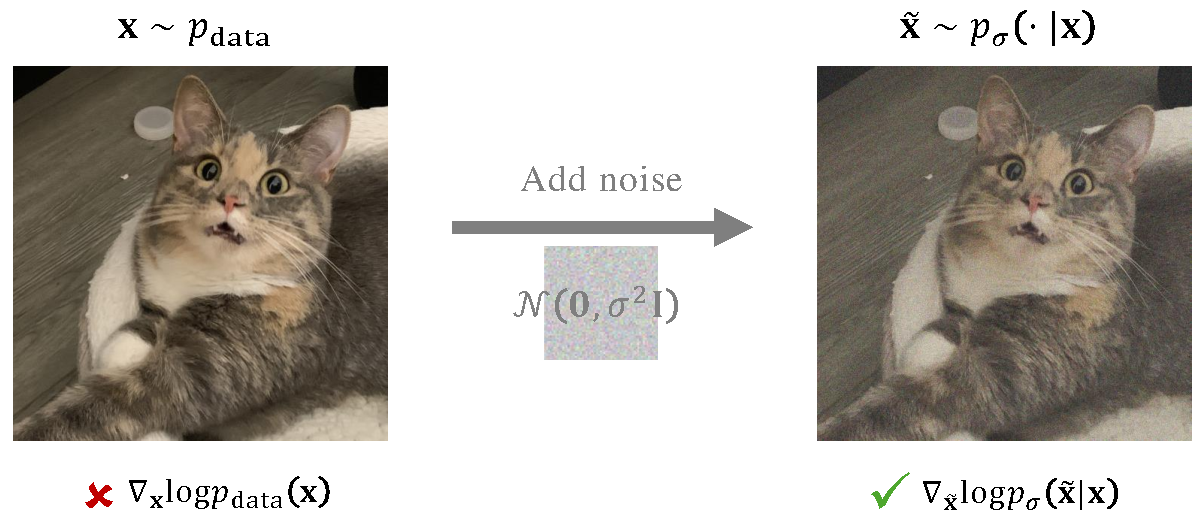
\includegraphics[width=0.8\linewidth]{Images/PartB/dsm-graph.pdf}
    \caption{\textbfs{通过条件化技巧的 DSM 示意图。} 通过用小的高斯加性噪声 $\mathcal{N}(\mathbf{0}, \sigma^2 \rmI)$ 扰动数据分布 $p_{\mathrm{data}}$，所得条件分布 $p_{\sigma}(\tilde{\rvx}|\rvx) = \mathcal{N}(\tilde{\rvx}; \rvx, \sigma^2 \rmI)$ 具有闭式形式的分数函数。
\figcredit{由作者绘制。}}
    \label{fig:dsm-graph}
\end{figure}


\paragraph{特例：加性高斯噪声。} 我们现在考虑常见情形：将方差为 $\sigma^2$ 的高斯噪声 $\mathcal{N}(\mathbf{0}, \sigma^2 \rmI)$ 加到每个数据点 $\rvx \sim p_{\text{data}}$ 上：
\[
\tilde{\rvx} = \rvx + \sigma \bm{\epsilon}, \quad \bm{\epsilon} \sim \mathcal{N}(\mathbf{0}, \rmI),
\]
使得受损数据 $\tilde{\rvx}$ 服从
\[
p_{\sigma}(\tilde{\rvx}|\rvx) = \mathcal{N}(\tilde{\rvx}; \rvx, \sigma^2 \rmI).
\]
在此设置下，条件分数解析地给出为
\[
\nabla_{\tilde{\rvx}} \log p_{\sigma}(\tilde{\rvx}|\rvx) = \frac{\rvx - \tilde{\rvx}}{\sigma^2}.
\]
因此，DSM 损失简化为：
\begin{mdframed}
\begin{align}\label{eq:gaussian-dsm}
\begin{aligned}
    \mathcal{L}_{\text{DSM}}(\bm{\phi}; \sigma) &= \frac{1}{2} \mathbb{E}_{\rvx, \tilde{\rvx}|\rvx} \left[ \norm{\rvs_{\bm{\phi}}(\tilde{\rvx}; \sigma) - \frac{\rvx - \tilde{\rvx}}{\sigma^2}}_2^2 \right] \\
    &= \frac{1}{2} \mathbb{E}_{\rvx, \bm{\epsilon}} \left[ \norm{\rvs_{\bm{\phi}}(\rvx + \sigma \bm{\epsilon}; \sigma) + \frac{\bm{\epsilon}}{\sigma}}_2^2 \right],
\end{aligned}
\end{align}
\end{mdframed}
其中 $\bm{\epsilon} \sim \mathcal{N}(\mathbf{0}, \rmI)$。这一目标构成了（基于分数的）扩散模型的核心。



当噪声水平 $\sigma$ 较小时，高斯平滑的边缘分布
$p_\sigma = p_{\mathrm{data}} * \mathcal{N}(\bm{0},\sigma^2 \rmI)$，
因此它们的高密度区域和分数几乎重合：
$\nabla_{\tilde{\rvx}} \log p_\sigma(\tilde{\rvx}) \approx \nabla_\rvx \log p_{\mathrm{data}}(\rvx)$。
因此，沿带噪分数方向
$\nabla_{\tilde{\rvx}} \log p_\sigma$ 迈出一小步，会将带噪样本移向干净分布本质上相同的高似然区域，
这与 \Cref{subsec:training-sm} 中总结的分数匹配的直觉类似。
相比之下，当 $\sigma$ 较大时，平滑会``过度简化''景观：
$p_\sigma$ 抹平了局部模态，其分数主要把样本拉向全局质量
（想象向均值的收缩），产生可能过度平滑的粗糙去噪。
然而在实践中，DSM 通常假设注入的噪声较小且温和。


为了更好地理解为什么该目标自然对应于一个``去噪''过程，
我们在 \Cref{subsec:why-dsm-denoising-tweedie,subsec:why-dsm-denoising-sure} 中对此讨论进行了展开。


% \se{i think it's important to explain why this is denoising. there's also a reasonable intuition where the best way to denoise is to locally maximize the log-likelihood of the nosy distribution. here it's probably good to at least mention Tweedie's formula, and perhaps Stein's unbiased risk estimator.
% probably worth mentioning that the same idea applies to higher order gradients, and in general to any linear operator
% }



\subsection{采样} 一旦我们在噪声水平 $\sigma$ 下有了训练好的分数模型 $\rvs_{\bm{\phi}^\times}(\tilde{\rvx}; \sigma)$，我们就可以通过用所学模型替代真实分数、用 Langevin 动力学来生成样本。更新规则为：
\begin{align}\label{eq:score-langevin-emp-dsm}
   \tilde{\rvx}_{n+1} = \tilde{\rvx}_n + \eta \underbrace{\rvs_{\bm{\phi}^\times}(\tilde{\rvx}_n; \sigma)}_{\approx \nabla_{\tilde{\rvx}} \log p_\sigma(\tilde{\rvx}_n)} + \sqrt{2\eta}    \bm{\epsilon}_n, \quad \bm{\epsilon}_n \sim \mathcal{N}(\mathbf{0}, \rmI),
\end{align}
其中 $n = 0, 1, 2, \dots$，从初始值 $\tilde{\rvx}_0$ 开始。若 $\sigma$ 足够小，则在足够多次迭代后，$\tilde{\rvx}_n$ 近似于来自 $p_{\text{data}}$ 的样本。


\paragraph{噪声注入的优势。}
我们还要指出，与 \Cref{eq:sm} 中的普通分数匹配相比，注入高斯噪声以形成 $p_\sigma$（例如 \Cref{eq:gaussian-dsm}）具有两个关键优势~\citep{song2019generative}：
\begin{itemize}
  \item \textbfs{良定义的梯度。} 噪声将数据扰动离开其低维流形，得到在 $\mathbb{R}^D$ 上具有完整支撑的分布 $p_\sigma$。因此，分数函数 $\nabla_{\tilde{\rvx}} \log p_\sigma(\tilde{\rvx})$ 处处良定义。
  \item \textbfs{改善的覆盖性。} 噪声平滑了模态之间的稀疏区域，提升了训练信号质量，并使 Langevin 动力学能够更有效地穿越低密度区域。
\end{itemize}


\subsection{为什么 DSM 是去噪：Tweedie 公式}\label{subsec:why-dsm-denoising-tweedie}

我们从\emph{Tweedie 公式}~\citep{efron2011tweedie} 开始，它为仅从带噪观测中进行去噪提供了有原则的基础。
具体而言，它指出：给定来自未知 $\rvx \sim p_{\mathrm{data}}$ 的单个高斯受损观测 $\tilde{\rvx}\sim\mathcal N(\,\cdot\,;\alpha\rvx,\sigma^2\mathrm{I})$，可以通过将 $\tilde{\rvx}$ 沿其带噪边缘分布（定义为下式）的分数
$\nabla_{\tilde{\rvx}}\log p_\sigma(\tilde{\rvx})$ 方向推动大小为 $\sigma^2$ 的一步，得到去噪估计（给定 $\tilde{\rvx}$ 时所有合理干净信号的平均）：
\[
p_\sigma(\tilde{\rvx}):= \int \mathcal{N}(\tilde{\rvx};\alpha \rvx,\sigma^2\mathrm{I})p_{\mathrm{data}}(\rvx)\diff\rvx.
\]
我们在下面正式陈述该命题。
\lemp{Tweedie 公式}{tweedie}{假设 $\rvx\sim p_{\mathrm{data}}$，且在给定 $\rvx$ 的条件下
$\tilde{\rvx}\sim\mathcal N(\,\cdot\,;\alpha\rvx,\sigma^2\mathrm{I})$，其中 $\alpha\neq0$。则 Tweedie 公式表明
 \begin{align}\label{eq:tweedie} 
 \alpha   \mathbb{E}_{\rvx \sim p(\rvx |\tilde\rvx)}\big[\rvx  \big|  \tilde\rvx\big] = \tilde\rvx + \sigma^2 \nabla_{\tilde\rvx} \log p_\sigma(\tilde\rvx), 
 \end{align} 其中期望是在给定 $\tilde\rvx$ 时 $\rvx$ 的后验分布 $p(\rvx |\tilde\rvx)$ 上取的。
}{
证明通过计算边缘分布
$p(\tilde\rvx)=\int p(\tilde\rvx|\rvx)p_{\mathrm{data}}(\rvx)\diff\rvx$ 的分数来完成。
在积分号下求导并利用条件密度的高斯形式，
可以直接得到一个表达式，整理后即得到将分数与后验均值联系起来的恒等式。详见 \Cref{app-sec:tweedie}。
}
Tweedie 公式在扩散模型中起着核心作用，在 DDPM 中引入了多层噪声。
它使得通过分数函数从带噪观测中估计干净样本成为可能，从而在分数预测与去噪器之间建立了一个基本联系：
\begin{equation*}
\underbrace{\mathbb{E} \left[\rvx|\tilde\rvx\right]}_{\substack{\text{denoiser}\\\text{estimated from }\tilde\rvx}}
= \frac{1}{\alpha}\left(\tilde\rvx + \sigma^2 \nabla_{\tilde\rvx} \log p_\sigma(\tilde\rvx)\right).
\end{equation*}

特别地，在带噪对数似然上以特定步长 $\sigma^2$
进行单步梯度上升，就得到去噪估计（条件平均的干净信号）。这使得
DSM 训练与去噪紧密相关：如果由 DSM 训练得到
$\rvs_\bphi(\tilde{\rvx})\approx
\nabla_{\tilde{\rvx}}\log p_\sigma(\tilde{\rvx})$，那么
\[
\frac{1}{\alpha}\left(\tilde{\rvx}+\sigma^2 \rvs_\bphi(\tilde{\rvx})\right)
\]
就是去噪器。

\paragraph{（可选）高阶 Tweedie 公式。} 经典的 Tweedie 公式通过梯度 $\nabla_{\tilde{\rvx}}\log p(\tilde{\rvx})$ 表达后验均值 $\E[\rvx_0|\tilde{\rvx}]$。
高阶扩展~\citep{meng2021estimating} 通过 $\log p(\tilde{\rvx})$ 的高阶导数来表达后验协方差和更高阶累积量。

\subparagraph{带对数归一化因子 $\lambda(\tilde{\rvx})$ 的指数族设置。}
假设给定潜在自然参数 $\boldsymbol\eta\in\R^D$ 时 $\tilde{\rvx}$ 的条件分布属于一个自然指数族，写作
\[
q_\sigma(\tilde{\rvx}|\boldsymbol\eta)
=\exp\!\big(\boldsymbol\eta^\top \tilde{\rvx}-\psi(\boldsymbol\eta)\big)\,q_0(\tilde{\rvx}).
\]
这里 $q_0(\tilde{\rvx})$ 是\emph{基准测度}，即不依赖于 $\boldsymbol\eta$ 的部分；对于方差为 $\sigma^2\rmI$ 的加性高斯噪声它等于 $(2\pi\sigma^2)^{-D/2}\exp(-\|\tilde{\rvx}\|^2/2\sigma^2)$。
设 $p(\boldsymbol\eta)$ 为预先定义的潜在自然参数分布，它可以被视为重新参数化的干净数据分布（对于高斯位置模型，$\boldsymbol\eta=\rvx/\sigma^2$）。
观测到的带噪边缘分布为
\[
p_\sigma(\tilde{\rvx})=\int q_\sigma(\tilde{\rvx}|\boldsymbol\eta)\,p(\boldsymbol\eta)\diff\boldsymbol\eta.
\]
定义 $\tilde{\rvx}$ 处的\emph{对数配分}（对数归一化因子）为
\[
\lambda(\tilde{\rvx}) := \log p_\sigma(\tilde{\rvx})-\log q_0(\tilde{\rvx}).
\]
则给定 $\tilde{\rvx}$ 时 $\boldsymbol\eta$ 的后验为
\[
p(\boldsymbol\eta|\tilde{\rvx})
\ \propto\
\exp\!\big(\boldsymbol\eta^\top \tilde{\rvx}-\psi(\boldsymbol\eta)-\lambda(\tilde{\rvx})\big)\,p(\boldsymbol\eta),
\]
这表明，作为 $\tilde{\rvx}$ 的函数，后验具有指数族形式，其自然参数为 $\tilde{\rvx}$，充分统计量为 $\boldsymbol\eta$，对数配分为 $\lambda(\tilde{\rvx})$。

\subparagraph{$\lambda$ 的导数产生后验累积量。}
这里有两条简单的规则在起作用。
首先是归一化：对每个 $\tilde{\rvx}$，
\[
\int \exp\!\big(\boldsymbol\eta^\top \tilde{\rvx}-\psi(\boldsymbol\eta)-\lambda(\tilde{\rvx})\big)\,p(\boldsymbol\eta)\diff\boldsymbol\eta
=1.
\]
对该恒等式关于 $\tilde{\rvx}$ 求导会从指数项中提取出 $\boldsymbol\eta$ 的各次幂以及 $\lambda(\tilde{\rvx})$ 的导数；将结果置零，就得到 $\lambda$ 的导数与 $\boldsymbol\eta$ 的后验矩之间的等式。
其次是指数族的一个标准性质：对数配分是充分统计量的累积量生成函数。
因此
\[
\nabla_{\tilde{\rvx}}\lambda(\tilde{\rvx})=\E[\boldsymbol\eta|\tilde{\rvx}],\quad
\nabla_{\tilde{\rvx}}^{2}\lambda(\tilde{\rvx})=\Cov[\boldsymbol\eta|\tilde{\rvx}],\quad
\nabla_{\tilde{\rvx}}^{(k)}\lambda(\tilde{\rvx})=\kappa_k(\boldsymbol\eta|\tilde{\rvx})\quad(k\ge 3),
\]
其中 $\kappa_k$ 是给定 $\tilde{\rvx}$ 时随机向量 $\boldsymbol\eta$ 的 $k$ 阶\emph{条件累积量}，通过标准的矩-累积量关系得到。


这些就是高阶 Tweedie 公式。
特化到 $\boldsymbol\eta=\rvx/\sigma^2$ 的高斯位置模型，得到用 $\log p_\sigma(\tilde{\rvx})$ 的导数表示的熟悉形式：
\[
\E[\rvx|\tilde{\rvx}]
=\tilde{\rvx}+\sigma^2\nabla_{\tilde{\rvx}}\log p_\sigma(\tilde{\rvx}),
\qquad
\Cov[\rvx|\tilde{\rvx}]
=\sigma^2\mathrm I+\sigma^4\nabla_{\tilde{\rvx}}^{2}\log p_\sigma(\tilde{\rvx}),
\]
而更高阶的累积量按 $\log p_\sigma(\tilde{\rvx})$ 的高阶导数缩放。


已有若干研究探索了训练神经网络以估计高阶分数~\citep{meng2021estimating,lu2022maximum,lai2023fp}。相比之下，我们的目标是阐明它们与统计量之间的关系，方法论的细节请读者参阅这些工作。

\subsection{（可选）为什么 DSM 是去噪：SURE}\label{subsec:why-dsm-denoising-sure}


\paragraph{SURE（Stein 无偏风险估计）。}
概括地说，Stein 无偏风险估计（SURE）是一种允许在\emph{不知道干净信号}的情况下估计去噪器 $\rmD$ 的均方误差（MSE）的技术。
换言之，SURE 提供了一种在只有带噪数据可用时选择或训练去噪器的方法。

为清晰起见，考虑加性高斯噪声设置：
\[
\tilde{\rvx} = \rvx + \sigma \bm{\epsilon}, 
\qquad \bm{\epsilon} \sim \mathcal{N}(\mathbf{0},\rmI),
\]
其中 $\rvx \in \R^D$ 是未知的干净信号，$\tilde{\rvx}$ 是观测到的带噪版本。
去噪器是任意（弱可微的）映射 $\rmD:\R^D \to \R^D$，它产生 $\rvx$ 的估计 $\rmD(\tilde{\rvx})$。

自然的质量度量是条件 MSE
\[
R(\rmD;\rvx) := \E_{\tilde{\rvx}|\rvx}\left[\|\rmD(\tilde{\rvx})-\rvx\|_2^2 \,\big|\, \rvx\right].
\]
该量依赖于未知的真实值 $\rvx$，因此无法直接计算。
然而，Stein 恒等式（见 \Cref{app-sec:stein-identity}）给出了如下\emph{可观测的}替代量：
\begin{align}\label{eq:sure-obj}
    \mathrm{SURE}(\rmD;\tilde{\rvx})
    = \|\rmD(\tilde{\rvx})-\tilde{\rvx}\|_2^2
    + 2\sigma^2\,\nabla_{\tilde{\rvx}}\cdot \rmD(\tilde{\rvx})
    - D\sigma^2,
\end{align}
其中 $\nabla_{\tilde{\rvx}}\cdot \rmD(\tilde{\rvx})$ 表示 $\rmD$ 的散度。
我们强调，$\mathrm{SURE}(\rmD;\tilde{\rvx})$ 只需要带噪观测 $\tilde\rvx$，而不需要干净的 $\rvx$。

直观上，$\mathrm{SURE}$ 由两个互补的部分组成。
项 $\|\rmD(\tilde{\rvx})-\tilde{\rvx}\|^2$ 度量去噪器输出与带噪输入之间的距离；
单看这一项会低估真实误差，因为 $\tilde{\rvx}$ 已经被污染。
散度项起到修正作用：它刻画了去噪器对其输入微小扰动的敏感程度，
从而有效地把噪声引入的方差考虑在内。


重要的是，对任意固定但未知的 $\rvx$，
\[
\E_{\tilde{\rvx}|\rvx}\left[\mathrm{SURE}(\rmD;\rvx+\sigma\beps) \,\big|\, \rvx\right]
= R(\rmD;\rvx),
\]
其中期望是在高斯噪声 $\beps\sim\mathcal{N}(\bm{0},\rmI)$ 上取的。因此，最小化 SURE（在期望意义下或经验地）等价于最小化真实 MSE，
而只依赖带噪数据。
在实践中，对 $\rvx\sim p_{\mathrm{data}}$ 和污染噪声 $\beps$ 都取平均的 $\mathrm{SURE}$，
给出全局 MSE 风险的无偏估计。

\paragraph{与 Tweedie 公式及 Bayes 最优性的联系。}
设 $p_\sigma(\tilde{\rvx}) = \big(p_{\mathrm{data}} * \mathcal{N}(\mathbf{0}, \sigma^2 \rmI)\big)(\tilde{\rvx})$ 表示本节所考虑的带噪边缘分布。


SURE 是关于噪声（在给定 $\rvx$ 的条件下）的均方误差的无偏估计：
\[
\mathbb{E}_{\tilde{\rvx}| \rvx}\!\big[\mathrm{SURE}(\rmD; \tilde{\rvx})\big]
=
\mathbb{E}_{\tilde{\rvx}| \rvx}\!\big[\|\rmD(\tilde{\rvx})-\rvx\|^2\big].
\]
因此，由全期望定律（塔性质），最小化期望 SURE 等价于最小化 Bayes 风险
$\mathbb{E}_{(\rvx, \tilde{\rvx})}\big[\|\rmD(\tilde{\rvx})-\rvx\|^2\big]
=\mathbb{E}_{\tilde{\rvx}}\!\big[\mathbb{E}_{\rvx| \tilde{\rvx}}\!\big[\|\rmD(\tilde{\rvx})-\rvx\|^2\big]\big]$。这一分解给出了逐点优化：对几乎每个 $\tilde{\rvx}$，
\[
\rmD^*(\tilde{\rvx})
=\arg\min_{\mathbf z}\ \mathbb{E}_{\rvx| \tilde{\rvx}}\!\big[\|\mathbf z-\rvx\|^2\big]
=\mathbb{E}[\rvx| \tilde{\rvx}].
\]
因此，SURE 最优去噪器与 \Cref{subsec:why-dsm-denoising-tweedie} 中的 Bayes 估计量一致，并由 Tweedie 恒等式：
\begin{align}\label{eq:sure-tweedie-denoiser}
    \rmD^*(\tilde{\rvx})=\mathbb{E}[\rvx| \tilde{\rvx}]=\tilde{\rvx}+\sigma^2\nabla_{\tilde{\rvx}}\log p_\sigma(\tilde{\rvx}).
\end{align}




\paragraph{SURE 与分数匹配的关系。}
\Cref{eq:sure-tweedie-denoiser} 中的恒等式促使我们通过分数场来参数化去噪器 $\rmD$：
\[
\rmD(\tilde{\rvx})=\tilde{\rvx}+\sigma^2\rvs_{\bm\phi}(\tilde{\rvx};\sigma),
\]
其中 $\rvs_{\bm\phi}(\cdot;\sigma)$ 旨在近似带噪分数
$\nabla_{\tilde{\rvx}}\log p_\sigma(\cdot)$。
将 $\rmD(\tilde{\rvx})=\tilde{\rvx}+\sigma^2 \rvs_{\bm\phi}(\tilde{\rvx};\sigma)$ 代入 \Cref{eq:sure-obj} 得
\[
\frac{1}{2\sigma^4}\,\mathrm{SURE}(\rmD;\tilde{\rvx})
=
\Tr\!\big(\nabla_{\tilde{\rvx}} s_{\bm\phi}(\tilde{\rvx};\sigma)\big)
+\tfrac12\|\rvs_{\bm\phi}(\tilde{\rvx};\sigma)\|_2^2
+\text{const}(\sigma).
\]
因此，对 $\tilde{\rvx}\sim p_\sigma$ 取期望后，最小化 SURE
等价于（相差一个加性常数）在噪声水平 $\sigma$ 下、在 $p_\sigma$ 下取期望的最小化 Hyvärinen 替代
分数匹配目标（见 \Cref{eq:sm-alternative}）。
因此，两个目标共享相同的最小化解，即 \Cref{eq:sure-tweedie-denoiser} 中的去噪器。



\subsection{（可选）广义分数匹配}


\paragraph{动机。}
经典分数匹配、去噪分数匹配以及高阶变体的目标都是
\[
\frac{\mathcal L p(\rvx)}{p(\rvx)},\quad\text{for some density } p
\]
其中线性算子 $\mathcal L$ 作用于密度。
在经典情形 $\mathcal L=\nabla_{\rvx}$ 下，这给出
\[
\nabla_{\rvx}\log p(\rvx) = \frac{\nabla_{\rvx} p(\rvx)}{p(\rvx)}
\]
$\frac{\mathcal L p}{p}$ 结构允许通过分部积分去除归一化常数，得到一个只依赖于 $p$ 的样本和所学场 $\rvs_\bphi$ 的可处理目标。
这一观点催生了广义分数匹配框架。

\paragraph{广义 Fisher 散度。}
设 $p$ 为数据分布，$q$ 为任意模型分布。
对于作用在 $\rvx$ 的标量函数上的线性算子 $\mathcal L$，定义广义 Fisher 散度
\[
\mathcal D_{\mathcal L}(p \,\|\, q)
:= \int p(\rvx) 
\left\|
\frac{\mathcal L p(\rvx)}{p(\rvx)}
-
\frac{\mathcal L q(\rvx)}{q(\rvx)}
\right\|_2^2 \diff \rvx.
\]
若 $\mathcal L$ 是\emph{完备的}，即
\[
\frac{\mathcal L p_1}{p_1}=\frac{\mathcal L p_2}{p_2} \text{ a.e.}\quad \text{implies}\quad p_1=p_2 \text{ a.e.,}
\]
则 $\mathcal D_{\mathcal L}(p \,\|\, q)=0$ 可确定 $q=p$。
对于 $\mathcal L=\nabla_{\tilde\rvx}$，这恢复为经典 Fisher 散度（见 \Cref{eq:fisher}）。

\paragraph{分数参数化。}
在实践中，我们不对归一化密度 $q$ 建模。
相反，我们直接参数化一个向量场 $\rvs_\bphi(\rvx)$ 来近似广义分数 $\frac{\mathcal L p(\rvx)}{p(\rvx)}$。
考虑
\[
\mathcal D_{\mathcal L}\!\left(p \,\|\, \rvs_\bphi\right)
:= \mathbb E_{\rvx\sim p}\!\left[\left\|\,\rvs_\bphi(\rvx) - \frac{\mathcal L p(\rvx)}{p(\rvx)}\right\|_2^2\right].
\]
尽管 $\frac{\mathcal L p(\rvx)}{p(\rvx)}$ 未知，但``分部积分''使损失只依赖于 $\rvs_\bphi$。
设 $\mathcal L^\dagger$ 为 $\mathcal L$ 的伴随算子，定义为
\[
\int \big(\mathcal L f\big)^\top g
= \int f\,(\mathcal L^\dagger g)
\quad\text{for all test functions } f,g,
\]
当边界项消失时，它在形式上把 $\mathcal L$``移动''到积分另一侧。
展开平方并应用该恒等式，得到可处理的目标
\[
\mathcal L_{\text{GSM}}(\bphi)
= \mathbb E_{\rvx\sim p}\!\left[
\frac{1}{2}\,\|\rvs_\bphi(\rvx)\|_2^2
-
\big(\mathcal L^\dagger \rvs_\bphi\big)(\rvx)
\right] + \text{const},
\]
其中常数不依赖于 $\bphi$。我们只通过期望使用 $p$，因此广义分数匹配损失可以从训练数据得到经验估计量，与经典分数匹配完全一样。

对于 $\mathcal L=\nabla$，有 $\mathcal L^\dagger=-\nabla\!\,\cdot$，这恢复为 \Cref{eq:sm-alternative} 中 Hyvärinen 的分数匹配目标 $\mathbb E_p\!\big[\tfrac{1}{2}\|\rvs_\bphi\|_2^2 + \nabla\!\cdot \rvs_\bphi\big]$。

\paragraph{算子示例。}
\begin{itemize}
\item \textbfs{经典分数匹配。} 考虑 $\mathcal L = \nabla_{\rvx}$。
则广义分数退化为经典分数函数
\[
\frac{\mathcal L p(\rvx)}{p(\rvx)}
= \nabla_{\rvx}\log p(\rvx).
\]
\item \textbfs{去噪分数匹配。}
对于加性高斯噪声，定义算子
\[
(\mathcal L f)(\tilde{\rvx})
= \tilde{\rvx}\,f(\tilde{\rvx}) + \sigma^2\nabla_{\tilde{\rvx}} f(\tilde{\rvx}).
\]
则
\[
\frac{\mathcal L p_\sigma(\tilde{\rvx})}{p_\sigma(\tilde{\rvx})}
= \tilde{\rvx} + \sigma^2\nabla_{\tilde{\rvx}}\log p_\sigma(\tilde{\rvx})
= \mathbb E[\rvx_0|\tilde{\rvx}],
\]
其中 $p_\sigma(\tilde{\rvx}):= \int \mathcal{N}(\tilde{\rvx};\alpha \rvx_0,\sigma^2\mathrm{I})p_{\mathrm{data}}(\rvx)\diff\rvx$ 且 $\tilde\rvx=\rvx+\sigma\beps$。这正是 Tweedie 恒等式。
用该算子最小化 $\mathcal L_{\text{GSM}}$ 会训练 $\rvs_\bphi$ 去近似去噪器，恢复去噪分数匹配目标。


\item \textbfs{高阶目标。}
在 $\mathcal L$ 内部堆叠导数会暴露 $\nabla^2\log p$ 及更高阶导数，它们与后验协方差和高阶累积量对齐。
\end{itemize}


\paragraph{扩展与用例。}
广义分数匹配从连续变量扩展到离散设置，包括语言建模\citep{meng2022concrete,lou2024discrete}。它还启发了产生去噪式目标的、受分数启发的训练。这种算子视角统一了一系列目标，允许从数据进行经验估计，并通过适当选择 $\mathcal L$ 为设计损失函数提供了一般原则.




\clearpage
\newpage


\section{\texorpdfstring{去噪分数匹配的多噪声层级（NCSN）}{去噪分数匹配的多噪声层级（NCSN）}}\label{sec:SMLD}

\subsection{动机}
向数据分布中加入单一固定方差的高斯噪声在一定程度上平滑了它，但只在一个噪声水平上训练基于分数的模型会引入关键局限。在低噪声注入水平下，由于低密度区域的梯度消失，Langevin 动力学难以在多模态分布中穿越模态。相反，在高噪声水平下，采样变得更容易，但模型只能捕捉到粗略结构，导致样本模糊、缺乏精细细节。此外，Langevin 动力学在高维空间中可能收敛缓慢甚至失败。由于它依赖对数密度的梯度进行引导，糟糕的初始化（尤其是在平台区域或鞍点附近）可能阻碍探索，或使采样器被困在单一模态中。


\begin{figure}[ht!]
    \centering
    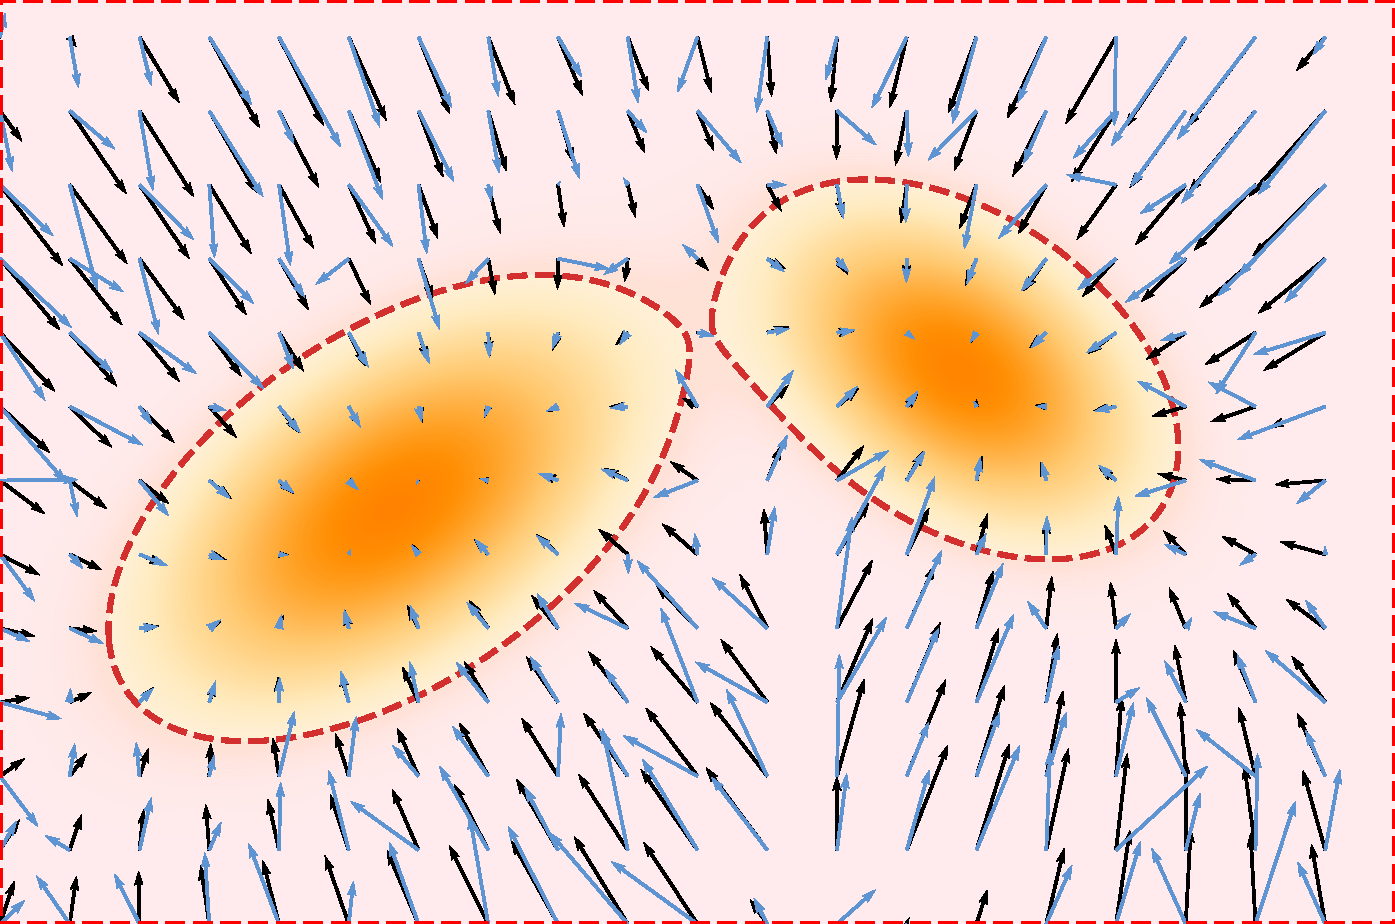
\includegraphics[width=0.85\linewidth]{Images/PartB/score_function_acc.pdf}
    \caption{\textbfs{SM 不准确性的示意图（重访 \Cref{fig:sm-illustration}）。} 红色区域表示由于样本覆盖有限而可能分数估计不准的低密度区域，而高密度区域往往产生更准确的估计。 \figcredit{由作者绘制。}}
    \label{fig:sm-acc-illustration}
\end{figure}


为应对这些挑战，\citet{song2019generative} 提出向数据分布中注入多个水平的高斯噪声，并联合训练一个噪声条件分数网络（NCSN）来估计一系列噪声尺度下的分数函数。在生成时，Langevin 动力学以噪声退火的方式应用：从高噪声水平开始以实现粗略探索，然后逐步细化到低噪声水平以恢复精细细节。




\begin{figure}[th]
    \centering
    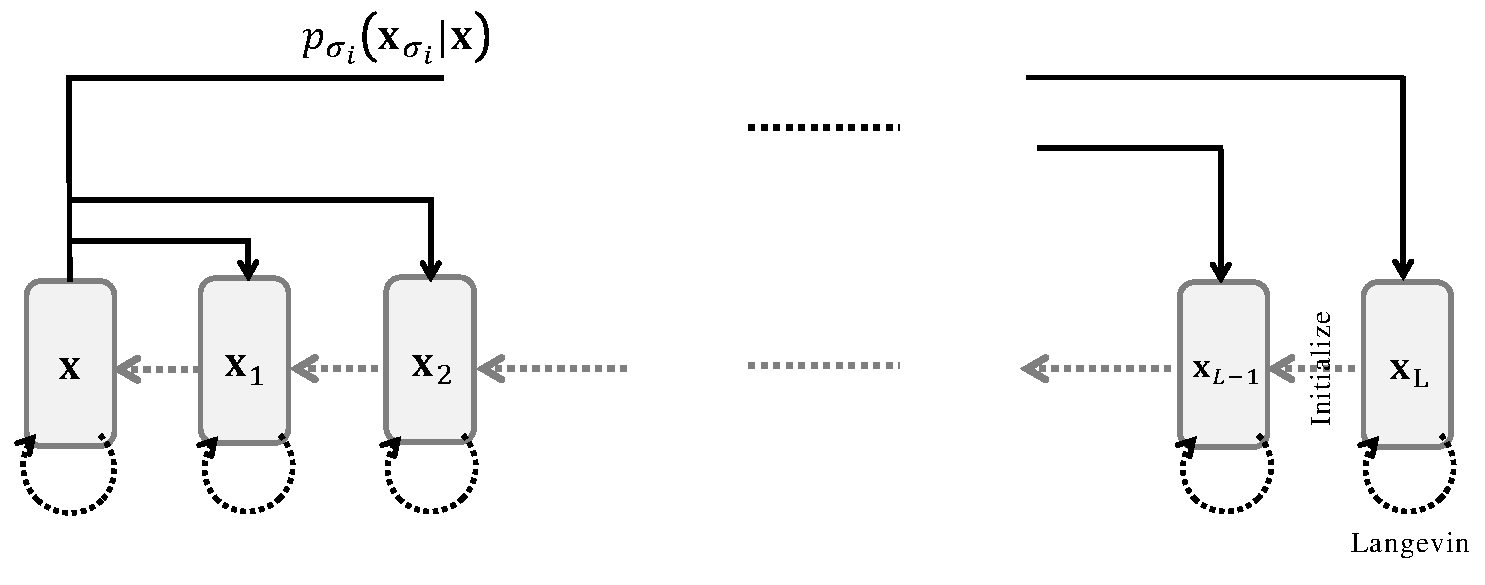
\includegraphics[width=0.95\linewidth]{Images/PartB/ncsn-graph.pdf}
    \caption{\textbfs{NCSN 示意图。} 前向过程用多层加性高斯噪声 $p_{\sigma}(\rvx_{\sigma} | \rvx)$ 扰动数据。生成（虚线）通过在每个噪声层进行 Langevin 采样来进行，并使用当前层的结果作为下一层（更小方差）采样的初始化。 \figcredit{由作者绘制。}}
    \label{fig:smld-ddpm-graphical-model}
\end{figure}


\subsection{训练}
为克服在单一噪声水平上训练基于分数模型的局限，\citet{song2019generative} 提出向数据分布中加入多个水平的高斯噪声。具体地，选择一系列 $L$ 个噪声水平 $\{\sigma_i\}_{i=1}^L$，使得
\[
0 < \sigma_1 < \sigma_2 < \cdots < \sigma_L,
\]
其中 $\sigma_1$ 足够小以保留数据的大部分精细细节，而 $\sigma_L$ 足够大以充分平滑分布，从而便于训练。

每个带噪样本通过扰动干净数据点 $\rvx \sim p_{\text{data}}$ 构造为 $\rvx_{\sigma} = \rvx + \sigma \bm{\epsilon}$，其中 $ \bm{\epsilon} \sim \mathcal{N}(\bm{0}, \rmI)$。这定义了
\vspace{-0.4cm}
\subparagraph{扰动核：}
\[
p_{\sigma}(\rvx_{\sigma} | \rvx) := \mathcal{N}(\rvx_{\sigma}; \rvx, \sigma^2 \rmI),
\]
它诱导出
\vspace{-0.4cm}
\subparagraph{边缘分布：}
\[
p_\sigma(\rvx_{\sigma}) = \int p_{\sigma} (\rvx_{\sigma} | \rvx)    p_{\text{data}}(\rvx) \diff \rvx,
\]
在每个噪声水平 $\sigma$ 处。它表示高斯平滑后的数据分布。

\paragraph{NCSN 的训练目标。}

目标是训练一个噪声条件分数网络 $\rvs_{\bm{\phi}}(\rvx, \sigma)$，以估计所有 $\sigma \in \{\sigma_i\}_{i=1}^L$ 的分数函数 $\nabla_{\rvx} \log p_\sigma(\rvx)$。这是通过在所有噪声水平上最小化 DSM 目标来实现的：
\begin{align}\label{eq:nscn}
\mathcal{L}_{\text{NCSN}}(\bm{\phi}) := \sum_{i=1}^{L} \lambda(\sigma_i)   \mathcal{L}_{\text{DSM}}(\bm{\phi}; \sigma_i),
\end{align}
其中
\begin{align*}
\mathcal{L}_{\text{DSM}}(\bm{\phi}; \sigma) 
= \frac{1}{2} \mathbb{E}_{\rvx \sim p_{\text{data}}(\rvx),   \tilde{\rvx} \sim p_{\sigma}(\tilde{\rvx} | \rvx)} 
\left[ \norm{\rvs_{\bm{\phi}}(\tilde{\rvx}, \sigma) - \left( \frac{\rvx - \tilde{\rvx}}{\sigma^2} \right)}_2^2 \right],
\end{align*}
且 $\lambda(\sigma_i)>0$ 是每个尺度的加权函数。

最小化该目标得到分数模型 $\rvs^*(\rvx, \sigma)$，它在每个噪声水平恢复真实分数：
\[
\rvs^*(\cdot, \sigma) = \nabla_{\rvx} \log p_\sigma(\cdot),  \quad \text{for all } \sigma \in \{\sigma_i\}_{i=1}^L,
\]
因为它本质上是 DSM 最小化（见定理~\ref{thm:sm-dsm}）。
% \se{discuss replationship with ddpm loss}


\paragraph{与 DDPM 损失的关系。}
设 $\rvx_\sigma=\rvx+\sigma\boldsymbol{\epsilon}$，其中 $\boldsymbol{\epsilon}\sim\mathcal{N}(\mathbf{0},\mathbf{I})$，并设 $p_\sigma$ 表示边缘分布。由 Tweedie 公式，
\[
\nabla_{\rvx_\sigma}\log p_\sigma(\rvx_\sigma)
= -\frac{1}{\sigma} \E \left[\boldsymbol{\epsilon} \middle|  \rvx_\sigma\right].
\]
因此 NCSN 的最优解是真实分数 $\rvs^*(\rvx_\sigma,\sigma)=\nabla_{\rvx_\sigma}\log p_\sigma(\rvx_\sigma)$，而 DDPM 损失 \Cref{eq:ddpm-simple-loss} 下的 Bayes 最优噪声预测器是 $\boldsymbol{\epsilon}^*(\rvx_\sigma,\sigma)=\E[\boldsymbol{\epsilon}|\rvx_\sigma]$。它们通过下式完全等价
\[
\rvs^*(\rvx_\sigma,\sigma) = - \frac{1}{\sigma} \boldsymbol{\epsilon}^*(\rvx_\sigma,\sigma),
\qquad
\boldsymbol{\epsilon}^*(\rvx_\sigma,\sigma) = - \sigma \rvs^*(\rvx_\sigma,\sigma).
\]
在 DDPM 的扰动 \Cref{eq:ddpm-perturbation}（离散指标 $i$）中，
\[
\rvx_i = \bar{\alpha}_i \rvx_0 + \sqrt{1 - \bar{\alpha}_i^2}
\]
同一关系给出
\[
\rvs^*(\rvx_i,i)= -\frac{1}{\sigma_i} \E \left[\boldsymbol{\epsilon} \middle|  \rvx_i\right],
\]
因此最小化 \Cref{eq:ddpm-simple-loss} 学习的是 $\boldsymbol{\epsilon}$ 的条件去噪器，它是噪声水平 $i$ 处真实分数的一个带缩放的重新参数化。

我们将在 \Cref{ch:all-equivalent} 中系统地比较和总结这种参数化的等价性。



\subsection{采样} 
\begin{algorithm}[th]
\caption{\label{alg:smld} 退火 Langevin 动力学}
\begin{algorithmic}[1]
\Require 已训练的分数 $\rvs_{\bm{\phi}^\times}(\cdot, \sigma_\ell)$、步长 $\eta_\ell$ 以及每个噪声水平 $\ell = L, \dots, 2$ 的 Langevin 迭代预算 $N_\ell$
\State $\rvx^{\sigma_L} \sim \mathcal{N}(\mathbf{0}, \mathbf{I})$
\For{$\ell = L, \dots, 2$}
    \State $\tilde{\rvx}_0 \gets \rvx^{\sigma_\ell}$
    \Statex\Comment{用上一噪声层的输出初始化 Langevin}
    \For{$n = 0$ \textbf{to} $N_\ell - 1$}
        \State $\bm{\epsilon}_n \sim \mathcal{N}(\mathbf{0}, \mathbf{I})$
        \State $\tilde{\rvx}_{n+1} \gets \tilde{\rvx}_n + \eta_\ell \rvs_{\bm{\phi}^\times}(\tilde{\rvx}_n, \sigma_\ell) + \sqrt{2\eta_\ell} \bm{\epsilon}_n$
    \EndFor
    \State $\rvx^{\sigma_{\ell-1}} \gets \tilde{\rvx}_{N_\ell}$
    \Statex \Comment{输出用作下一噪声层的初始化}
\EndFor
\Ensure $\rvx^{\sigma_1}$ 
\end{algorithmic}
\end{algorithm}


在多个噪声水平上都有训练好的分数网络后
\[
\rvs_{\bm{\phi}^\times}(\cdot, \sigma_1), \quad\rvs_{\bm{\phi}^\times}(\cdot, \sigma_2), \quad \cdots, \quad \rvs_{\bm{\phi}^\times}(\cdot, \sigma_{L-1}), \quad    \rvs_{\bm{\phi}^\times}(\cdot, \sigma_L),
\]
% \se{this notation is weird}\jcc{do you meant the notation of $\bm{\phi}^\times$ is weird, which i was thoroughly using $\bm{\phi}^\times$ to denote a trained network? }
被称为\emph{退火 Langevin 动力学}~\citep{song2019generative} 的采样过程通过从高噪声水平 $\sigma_L$ 逐步去噪到低噪声水平 $\sigma_1 \approx 0$ 来生成数据。

从高斯噪声 $\rvx^{\sigma_L} \sim \mathcal{N}(\bm{0}, \rmI)$ 开始，该算法在每个噪声水平 $\sigma_\ell$ 应用 Langevin 动力学，以近似地从扰动分布 $p_{\sigma_\ell}(\rvx)$ 中采样。$\sigma_\ell$ 层的输出用于为下一个更低噪声水平 $\sigma_{\ell-1}$ 提供\emph{更好的初始化}。

在每个水平，Langevin 动力学迭代地更新：
\[
\tilde{\rvx}_{n+1} = \tilde{\rvx}_n + \eta_\ell \rvs_{\bm{\phi}^\times}(\tilde{\rvx}_n, \sigma_\ell) + \sqrt{2\eta_\ell} \bm{\epsilon}_n, \quad \bm{\epsilon}_n \sim \mathcal{N}(\bm{0}, \rmI),
\]
从 $\tilde{\rvx}_0 := \rvx^{\sigma_\ell}$ 开始。步长通常按噪声水平缩放：
\[
\eta_\ell = \delta \cdot \frac{\sigma_\ell^2}{\sigma_1^2}, \quad \text{for some fixed } \delta > 0.
\]
这种噪声退火的细化一直进行到最低噪声水平 $\sigma_1$，在那里得到最终样本 $\rvx^{\sigma_1}$。通过逐步地把上一层的输出作为下一层更好的初始化，这一策略实现了对复杂数据分布更有效的探索和更优的覆盖。\Cref{alg:smld} 总结了该过程。

\paragraph{NCSN 采样速度慢。}
NCSN 使用退火 MCMC（通常是 Langevin 动力学）跨噪声尺度 $\{\sigma_i\}_{i=1}^L$ 生成样本。
对每个尺度 $\sigma_i$，它执行 $K$ 次``用分数 $\rvs_{\bm{\phi}^\times}(\tilde{\mathbf{x}}_n,\sigma_i)$ 加上一个小随机扰动来更新 $\tilde{\mathbf{x}}_n$''形式的迭代更新，每次都需要通过分数网络的一次前向传播。两个因素使得 $L \times K$ 必须很大：
\begin{enumerate}
    \item[(i)] \textbfs{局部精度与稳定性：} 所学到的分数只对小扰动可靠，需要小步长和每个噪声水平多次迭代以避免偏差或不稳定；
    \item[(ii)] \textbfs{高维下混合缓慢：} 局部 MCMC 移动低效地探索多模态、高维目标，需要大量迭代才能到达典型数据区域。
\end{enumerate}
由于更新严格串行（每次迭代依赖于前一次），且每次都需要昂贵的网络计算，总代价是 $\mathcal{O}(L  K)$ 次串行网络传播，使采样在计算上很慢。

% \newpage

% \paragraph{Link Between Fisher Divergence and KL Divergence.} Maximum likelihood fits $q_\bphi$ by minimizing $\mathcal{D}_\mathrm{KL}(p\|q_\bphi)=\mathbb{E}_{p}[\log p-\log q_\bphi]$. Score matching fits $q_\bphi$ by minimizing the Fisher divergence $\mathcal{D}_{\mathrm F}(p\|q_\bphi)=\mathbb{E}_{p} \big[\|\nabla \log p-\nabla \log q_\bphi\|^2\big]$. They agree at the optimum ($p=q_\bphi$) but use different discrepancy measures. The key bridge is that when you smooth both distributions with Gaussian noise, $p_t=p*\mathcal N(\bm{0},t\rmI)$ and $q_t=q_\bphi*\mathcal N(\bm{0},t\rmI)$, the KL decreases along the noise scale at a rate given by Fisher:
% \[
% \frac{\diff}{\diff t}\mathcal{D}_\mathrm{KL}(p_t\|q_t)=-\tfrac12 \mathcal{D}_{\mathrm F}(p_t\|q_t).
% \]
% So Fisher is the instantaneous decay rate of KL under Gaussian smoothing. Moreover, for many smooth, near Gaussian targets (those satisfying a log Sobolev inequality), minimizing $\mathcal{D}_{\mathrm F}(p\|q_\bphi)$ controls $\mathcal{D}_\mathrm{KL}(p\|q_\bphi)$ via a bound like $\mathcal{D}_\mathrm{KL}(p\|q_\bphi)\lesssim \mathcal{D}_{\mathrm F}(p\|q_\bphi)$. In practice, this explains why score matching (and its denoising version used in diffusion models) can learn models with good likelihood while avoiding the intractable partition function: it matches scores directly, which do not depend on normalization, yet it still pushes down KL through the smoothing identity.



\clearpage
\newpage

\section{小结：NCSN 与 DDPM 的比较视角}

我们首先在 \Cref{fig:smld-ddpm-graphical-model} 中比较 NCSN 和 DDPM 的图模型，关键异同总结在 \Cref{tb:comparison-smld-ddpm} 中。


\begin{table}[th]
  \caption{NCSN 与 DDPM 的比较}
  \small
  \centering
  \resizebox{\textwidth}{!}{
  \begin{tabular}{cccc}
     \toprule
    
         &   \textbfs{NCSN}   & \textbfs{DDPM}  \\
        \midrule
    $\rvx_{i+1}|\rvx_{i}$ & 推导为 $\rvx_{i+1} =  \rvx_i + \sqrt{\sigma^2_{i+1}-\sigma^2_{i}}\bm{\epsilon}$   &  \cc{15}定义为 $\rvx_{i+1} = \sqrt{1-\beta_{i}} \rvx_{i} + \sqrt{\beta_{i}}\bm{\epsilon}$  \\
      $\rvx_{i}|\rvx$   & \cc{15}定义为 $\rvx_{i} =  \rvx + \sigma_{i}\bm{\epsilon}$
       &  推导为 $\rvx_i = \bar{\alpha}_i\rvx + \sqrt{1 - \bar{\alpha}_i^2}\bm{\epsilon}$ \\
   $p_{\text{prior}}$   & $ \mathcal{N}(\bm{0}, \sigma_L^2\rmI)$    &  $\mathcal{N}(\bm{0}, \rmI)$  \\
   \midrule
        损失 
          &  
        $\mathbb{E}_{i} \mathbb{E}_{p_{\text{data}}(\rvx)} 
        \mathbb{E}_{\bm{\epsilon} \sim \mathcal{N}\left(\mathbf{0}, \rmI\right)}   
    \left[ \norm{\rvs_{\bm{\phi}}(\rvx_i, \sigma_i) +   \frac{\bm{\epsilon}}{\sigma_i}}_2^2 \right] $ 
            &  $      \mathbb{E}_{i}\mathbb{E}_{p_{\text{data}}(\rvx)} \mathbb{E}_{\bm{\epsilon}\sim \mathcal{N}(\bm{0},\rmI)}\left[ \norm{\bm{\epsilon}_{\bm{\phi}}(\rvx_i, i) - \bm{\epsilon}}_2^2 \right]$ \\
    \midrule
     采样   & \begin{tabular}{@{}c@{}} 逐层应用 Langevin 动力学；\\ 用输出初始化下一层 \end{tabular}  &  \begin{tabular}{@{}c@{}}沿马尔可夫链遍历 \\ $p_{\bm{\phi}^\times}(\rvx_{i-1} | \rvx_i)$   \end{tabular} \\
 \bottomrule
  \end{tabular}
  }
  \label{tb:comparison-smld-ddpm}
\end{table}

\paragraph{共同的瓶颈。}
尽管形式不同，NCSN 和 DDPM 都依赖于密集的时间离散化。这导致一个关键局限：采样往往需要数百甚至数千次迭代，使生成缓慢且计算密集。

\begin{question}\label{ques:dm-sampling-slow}
    我们如何加速扩散模型中的采样？
\end{question}

我们在 \Cref{ch:solvers}（开发更高效的采样器）、\Cref{ch:distillation}（将需要数百采样步骤的预训练扩散模型压缩为更少步骤的学生生成器）以及 \Cref{ch:fast-scratch}（研究如何在扩散启发的原则下直接从头学习快速的少步生成器）中回到这一挑战。

% \paragraph{What Lies Ahead?}

% Despite their seemingly different origins, NCSN and DDPM share a strikingly similar high-level philosophy. Both inject noise at multiple levels and train models to progressively denoise, enabling tractable learning through conditioning and effective generation via noise-annealed refinement. This principle of layering stochasticity and learning to reverse it step-by-step provides a powerful foundation for modeling complex data distributions. 

% In the next chapter, \Cref{ch:score-sde}, we step into the continuous-time world, where the boundary between DDPM and NCSN begins to blur, revealing a profound unification at the heart of diffusion modeling.

\newpage

\section{结语}\label{sec:ch3_cr}



本章勾勒了通向扩散模型的第二条主要路径，起点是根植于基于能量的模型（EBM）的分数视角。我们从识别 EBM 的核心挑战——难以处理的配分函数——开始，并引入分数函数 $\nabla_{\mathbf{x}}\log{p(\mathbf{x})}$ 作为完全绕开这一问题的有力工具。

我们的旅程从经典分数匹配走向其更具可扩展性和鲁棒性的变体——去噪分数匹配（DSM）。通过 DSM，我们看到了用噪声扰动数据如何带来可处理的训练目标，再次利用条件化策略来创建简单的回归目标。此外，我们通过 Tweedie 公式建立了分数估计与去噪行为之间的深刻联系，它表明分数提供了从带噪观测中估计干净信号所需的精确方向。


这一原理随后从单一噪声水平扩展到由噪声条件分数网络（NCSN）构成的连续体，NCSN 学习一个以多个噪声尺度为条件的单一分数模型，并通过退火 Langevin 动力学生成样本。在探索结束时，我们发现 NCSN 与来自变分视角的 DDPM 尽管起源不同，却共享惊人相似的结构和一个共同的瓶颈：缓慢的串行采样。



这种收敛并非巧合；它暗示着一种更深层的、统一的数学结构。这些离散时间模型的局限促使我们需要一个更一般的框架。在下一章中，我们将迈出这关键一步：
\begin{enumerate}
    \item 我们将进入连续时间视角，证明 DDPM 和 NCSN 都可以优雅地统一为由随机微分方程（SDE）描述的单一强大过程的不同离散化。
    \item 这一 Score SDE 框架将正式连接变分视角与基于分数的视角，把生成问题重新表述为求解微分方程的问题。
\end{enumerate}

这一统一视角不仅将提供深刻的理论清晰度，还将开启一类旨在解决采样缓慢这一根本挑战的先进数值方法。
\chapter{今日的扩散模型：Score SDE 框架}\label{ch:score-sde}

\epigraph{
    \textit{呈现物理定律只有一种精确的方式，那就是借助微分方程。它们的优势在于具有根本性，并且据我们所知是精确的。
}}{Richard P. Feynman}



到目前为止，我们已经从两个视角研究了扩散模型：变分视角与分数基视角，后者自然地从 EBM 的表述中产生。现在我们迈出下一步，进入\emph{连续时间框架}。其核心是 \emph{Score SDE}，它是将 DDPM 与 NCSN 统一为单一表述的连续极限。这一视角极为强大，因为它以基于微分方程（DE）的、干净而富有原理的描述来扩展离散更新。
在这一视角下，生成退化为随时间求解一个 DE。这使我们能够直接应用数值分析中的工具：例如，基本的 Euler 方法可以模拟其动力学，而更高级的求解器则能改善稳定性与效率。
通过在连续时间下工作，我们还获得了更丰富的数学结构，以及用于理解、分析和改进扩散模型的统一基础。本专著将进一步发展这一视角。






\newpage

\section{Score SDE：其原理}\label{sec:dm-today}
% The use of multiple noise scales has been a crucial ingredient in the success of NCSN and DDPM frameworks. In this section, we introduce the foundation of the \emph{Score SDE}~\citep{song2020score}, which elevates this idea by considering a continuum of noise levels which this continuous-time limit of forward/reverse diffusion model perspective had been pointed out in \citep{sohl2015deep}. Instead of perturbing data using a fixed or finite set of noise magnitudes, \citet{song2020score} propose a formulation in which the data distribution evolves smoothly over time according to an SDE, as the noise level continuously increases. This continuous-time perspective not only unifies prior discrete models, but also enables a principled and flexible framework for generative modeling via continuous-time processes.
\begin{figure}
    \centering
    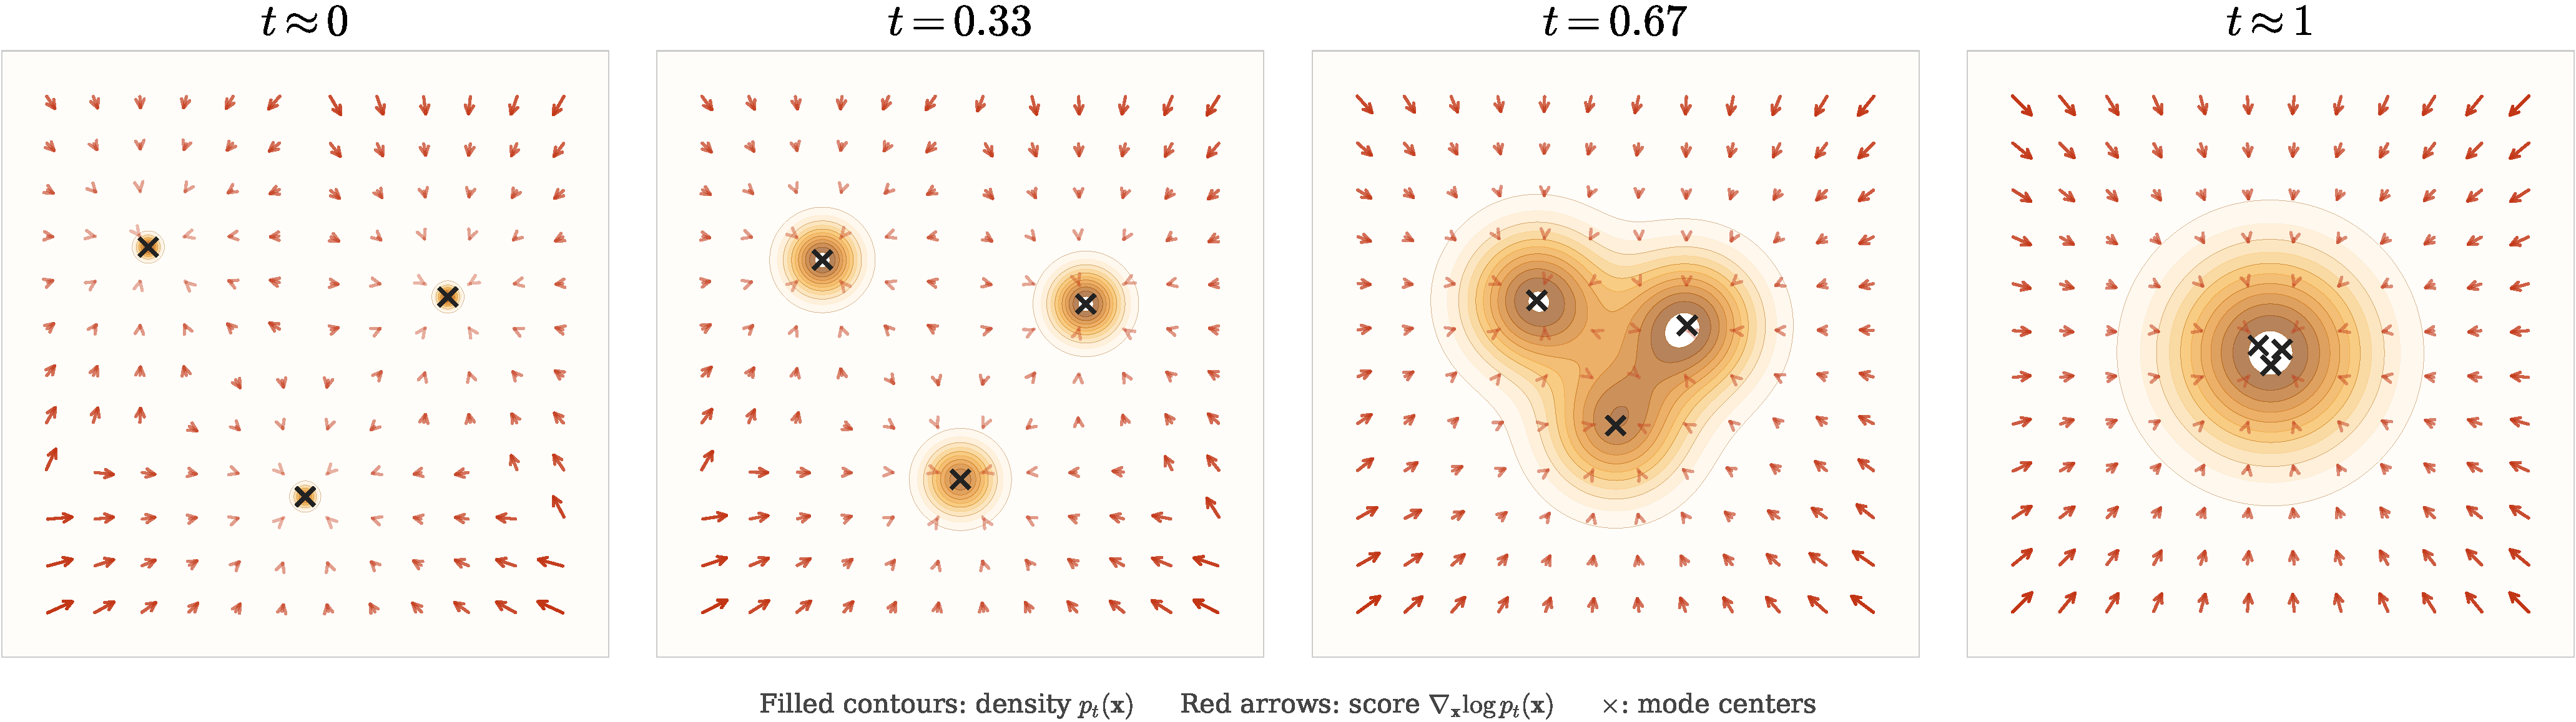
\includegraphics[width=\linewidth]{Images/PartB/score_landscape_2d.pdf}
    \caption{\textbfs{时间依赖分数景观的示意图。}
随着噪声水平增加，受扰密度 $p_t(\rvx)$ 从集中于数据模态附近的多峰分布（数据）演化为宽阔的、几乎单峰的分布（先验）。
相应地，分数场 $\nabla_{\rvx}\log p_t(\rvx)$ 从将样本拉向邻近模态的尖锐局部向量场，变为指向整体质心的平滑全局场。
这一时间依赖的分数场是基于分数的扩散模型（即 Score SDE）所学习的关键对象。 \figcredit{由作者借助 AI 辅助编程绘制。}}
    \label{fig:time-dependent-score}
\end{figure}

% The use of multiple noise scales has been a crucial ingredient in the success of NCSN and DDPM frameworks. In this section, we introduce the foundation of the \emph{Score SDE}~\citep{song2020score}, which elevates this idea by considering a continuum of noise levels. A continuous-time limit of forward and reverse diffusion processes had already been noted by \citet{sohl2015deep}, but \citet{song2020score} make this perspective central by formulating the data evolution as a stochastic/ordinary differential equation, where the noise level increases smoothly over time. This continuous-time formulation not only unifies prior discrete-time models but also provides a principled and flexible foundation for generative modeling by casting it as the problem of solving differential equations.

多种噪声尺度的使用一直是 NCSN 与 DDPM 框架成功的关键因素。在本节中，我们介绍 \emph{Score SDE}~\citep{song2020score} 的基础，它通过考虑连续的噪声水平谱来提升这一思想。前向与反向扩散过程的连续时间极限早已被 \citet{sohl2015deep} 注意到，但 \citet{song2020score} 通过将数据演化表述为一个随机/常微分方程（其中噪声水平随时间平滑增加）使这一视角成为核心。这一表述的核心是\emph{时间依赖的分数函数} $\nabla_{\rvx}\log p_t(\rvx)$：在每个噪声水平~$t$，它指向当前含噪分布~$p_t$ 下密度更高的区域，而正是这个量决定了如何反转扩散过程。如 \Cref{fig:time-dependent-score} 所示，分数场从在小的~$t$ 时尖锐地收敛于各个数据模态，演变为在大的~$t$ 时平缓地指向全局中心。这一连续时间表述不仅统一了此前的离散时间模型，而且为生成式建模提供了富有原理且灵活的基础：在所有噪声水平上学习这一族分数函数，将生成问题归结为求解微分方程的问题。




% \se{might need to properly attribute the 2015 paper, they had a continuous time version there}

% \jcr{The use of multiple noise scales has been central to NCSN and DDPM. In this section we adopt the continuous-time view popularized by the \emph{Score SDE}~\citep{song2020score}, which models a continuum of noise levels via an SDE. A continuous-time perspective predates this:  provided  continuous-time limit and time-reversal perspective of variational-based diffusion model. Building on that foundation, \citet{song2020score} make the reverse-time dynamics explicit in terms of the score $\nabla_{\rvx}\log p_t(\rvx)$, thereby unifying DDPM and SMLD and enabling principled sampling with SDE/ODE solvers. We focus on this score-driven formulation below.
% }

\subsection{动机：从离散到连续时间过程}\label{subsec:scoresde-motivation}

% \se{either reintroduce the symbols, or refer to previous equations. i would probably reintroduce if you expect people to skip chapters}
我们重新审视 NCSN 与 DDPM 的前向噪声注入方案。NCSN 使用一组递增的噪声水平 $\{\sigma_i\}_{i=1}^L$。
每个干净样本 $\rvx_0 \sim p_{\mathrm{data}}$ 被扰动为
\[
\rvx_{\sigma_i} = \rvx_0 + \sigma_i \bm{\epsilon}_i, 
\qquad \bm{\epsilon}_i \sim \mathcal{N}(\bm{0}, \rmI).
\]
DDPM 则通过方差调度 $\{\beta_i\}_{i=1}^L$ 逐步注入噪声\footnote{在 \Cref{sec:ddpm} 中，DDPM 的前向步骤写作 $\rvx_i = \sqrt{1-\beta_i^2}\,\rvx_{i-1} + \beta_i\,\bm{\epsilon}_i$，其中 $\beta_i$ 表示注入噪声的标准差，且 $\alpha_i := \sqrt{1-\beta_i^2}$。在本章及全书中，我们遵循 \citet{song2020score} 的约定，其中 $\beta_i$ 表示注入噪声的方差，故 $\rvx_i = \sqrt{1-\beta_i}\,\rvx_{i-1} + \sqrt{\beta_i}\,\bm{\epsilon}_i$。两种约定通过 $\beta_i^{\textup{(here)}} = \bigl(\beta_i^{\textup{(Ch.\ \ref{ch:variational})}}\bigr)^2$ 相联系，并给出完全相同的动力学。}：
\[
\rvx_i = \sqrt{1 - \beta_i}\, \rvx_{i-1} + \sqrt{\beta_i}\, \bm{\epsilon}_i, 
\qquad \bm{\epsilon}_i \sim \mathcal{N}(\bm{0}, \rmI).
\]

我们在一个离散时间网格上将它们放在一起看待，其中从 $\rvx_t$ 到 $\rvx_{t+\Delta t}$ 的顺序更新形如\footnote{为方便起见，我们互换使用 $\rvx(t)$ 与 $\rvx_t$（其他时间依赖变量亦同理），用以表示时刻 $t$ 的样本。}：
\begin{align*}
    \text{\textbfs{NCSN:}} \,\,
    & \rvx_{t+\Delta t} = \rvx_t + \sqrt{\sigma_{t+\Delta t}^2 - \sigma_t^2} \bm{\epsilon}_t 
    &&\approx \rvx_t + \sqrt{\frac{\diff \sigma_t^2}{\diff t} \Delta t}  \bm{\epsilon}_t \\[0.5em]
    \text{\textbfs{DDPM:}} \,\,
    & \rvx_{t+\Delta t} = \sqrt{1 - \beta(t)\Delta t} \rvx_t + \sqrt{\beta(t)\Delta t} \bm{\epsilon}_t 
    &&\approx \rvx_t - \frac{1}{2} \beta(t) \rvx_t  \Delta t + \sqrt{\beta(t)\Delta t}  \bm{\epsilon}_t,
\end{align*}
其中 $\bm{\epsilon}_t \sim \mathcal{N}(\bm{0}, \rmI)$。有趣的是，这两个噪声注入过程都遵循一个共同的结构模式：
\begin{align}\label{eq:euler-discrete-sde}
    \rvx_{t+\Delta t} \approx \rvx_t + \rvf(\rvx_t, t) \Delta t + g(t) \sqrt{\Delta t}\, \bm{\epsilon}_t,
\end{align}
其中 $\rvf: \mathbb{R}^D \times \mathbb{R} \to \mathbb{R}^D$ 和 $g: \mathbb{R} \to \mathbb{R}$ 由下式给出：
\begin{align*}
    \text{\textbfs{NCSN:}} \quad 
    & \rvf(\rvx, t) = 0, \qquad g(t) = \sqrt{\frac{\diff \sigma^2(t)}{\diff t}} \\[0.5em]
    \text{\textbfs{DDPM:}} \quad 
    & \rvf(\rvx, t) = -\frac{1}{2} \beta(t)\, \rvx, \qquad g(t) = \sqrt{\beta(t)}.
\end{align*}


\begin{figure}
    \centering
    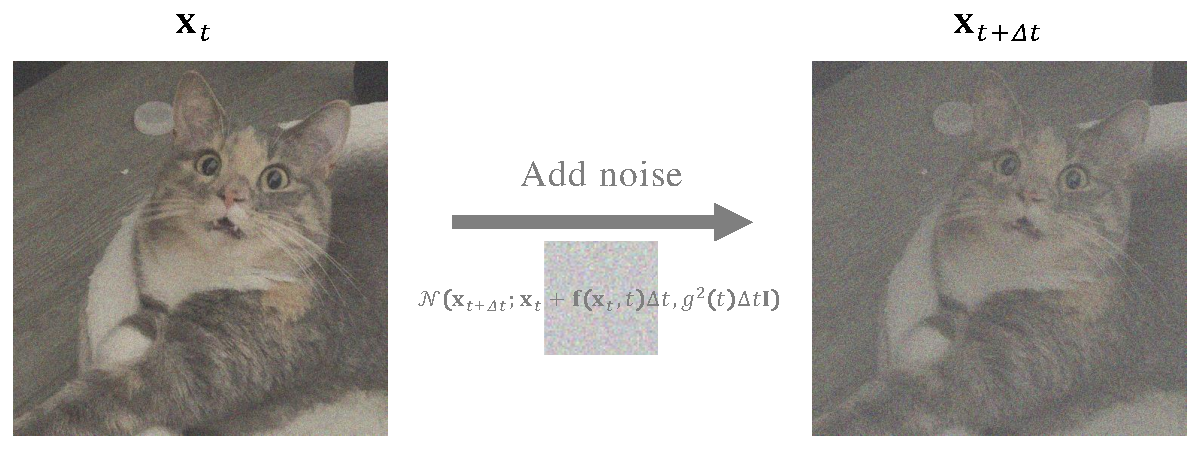
\includegraphics[width=0.9\linewidth]{Images/PartB/sde-forward-noise.pdf}
    \caption{\textbfs{离散时间加噪步骤的示意图。}它以均值漂移项 $\rvf(\rvx_t, t)$ 和扩散系数 $g(t)$ 从 $t$ 到 $t + \Delta t$ 添加噪声。 \figcredit{由作者绘制。}}
    \label{fig:sde-forward-noise}
\end{figure}

该表述对应如下高斯转移：
\begin{align}\label{eq:transition-forward-f-g}
    p(\rvx_{t+\Delta t} |\rvx_t) := \mathcal{N}\!\left(\rvx_{t+\Delta t}; \rvx_t + \rvf(\rvx_t, t)\Delta t,\, g^2(t)\Delta t\, \rmI\right),
\end{align}
其中，在不严格使用记号的情况下，我们将 $\rvx_t$ 视为固定样本，将 $\rvx_{t+\Delta t}$ 视为随机变量。

当 $\Delta t \to 0$（在概念上可理解为准备\emph{无穷多层}噪声）时，离散时间过程收敛为一个沿时间向前演化的连续时间 SDE\footnote{\Cref{eq:transition-forward-f-g} 中的前向核当 $\Delta t\to0$ 时收敛到相应 Itô SDE 的解。完整的严格证明依赖于高级结论，我们将其留待文献中讨论。}：
\begin{align*}
    \diff \rvx(t) = \rvf(\rvx(t), t) \diff t + g(t) \diff \rvw(t),
\end{align*}
其中 $\rvw(t)$ 是标准 Wiener 过程（或布朗运动）。
\rmkb{虽然此处并不需要完整的形式化定义，但 \emph{Wiener 过程}是一个连续时间随机过程 $ \rvw(t) $，它从零开始、具有独立增量，并满足对任意 $ s < t $，增量 $ \rvw(t) - \rvw(s) $ 服从均值为零、方差为 $ t - s $ 的正态分布。它表示独立高斯涨落随时间的累积，虽然它几乎必然连续，却处处不可微。

在一个无穷小时间区间 $[t, t + \diff t]$ 上，Wiener 过程的增量定义为
\[
\diff \rvw(t) := \rvw(t + \diff t) - \rvw(t),
\]
它被建模为均值为零、方差为 $\diff t$ 的高斯随机变量：
\[
\diff \rvw(t) \sim \mathcal{N}(\bm{0}, \diff t \rmI).
\]}

\Cref{app:sde-intro} 提供了 SDE 基础的简要介绍，\Cref{app:Ito} 中则有更深入的讨论。不过，我们可以在概念上按如下方式理解离散与连续表述之间的联系：
\begin{itemize}
    \item $\rvx(t+\Delta t) - \rvx(t) \approx \diff \rvx(t)$，
    \item $\Delta t \approx \diff t$，
    \item $\sqrt{\Delta t} \bm{\epsilon}_t \sim \mathcal{N}(\bm{0}, \Delta t \rmI) \approx \diff \rvw(t)$。
\end{itemize}
一旦指定了漂移项 $\rvf(\rvx,t)$ 与扩散系数 $g(t)$，前向时间 SDE 便自动诱导出一个反向时间 SDE，将终止时的噪声分布传输回数据分布。反向动力学仅包含一个未知项，令人惊讶的是，它正是\emph{每个连续时间水平上的分数函数}。这就把分数匹配确定为训练目标；一旦学得分数，采样便归结为用学得的分数对反向时间 SDE 进行数值积分。


\Cref{sec:scoresde-training-sampling} 给出了实际实现，但我们首先在 \Cref{subsec:forward-sde} 和 \Cref{subsec:reverse-sde} 中考察前向与反向过程的理论基础。




\subsection{前向时间 SDE：从数据到噪声}\label{subsec:forward-sde}
\begin{figure}[th!]
    \centering
    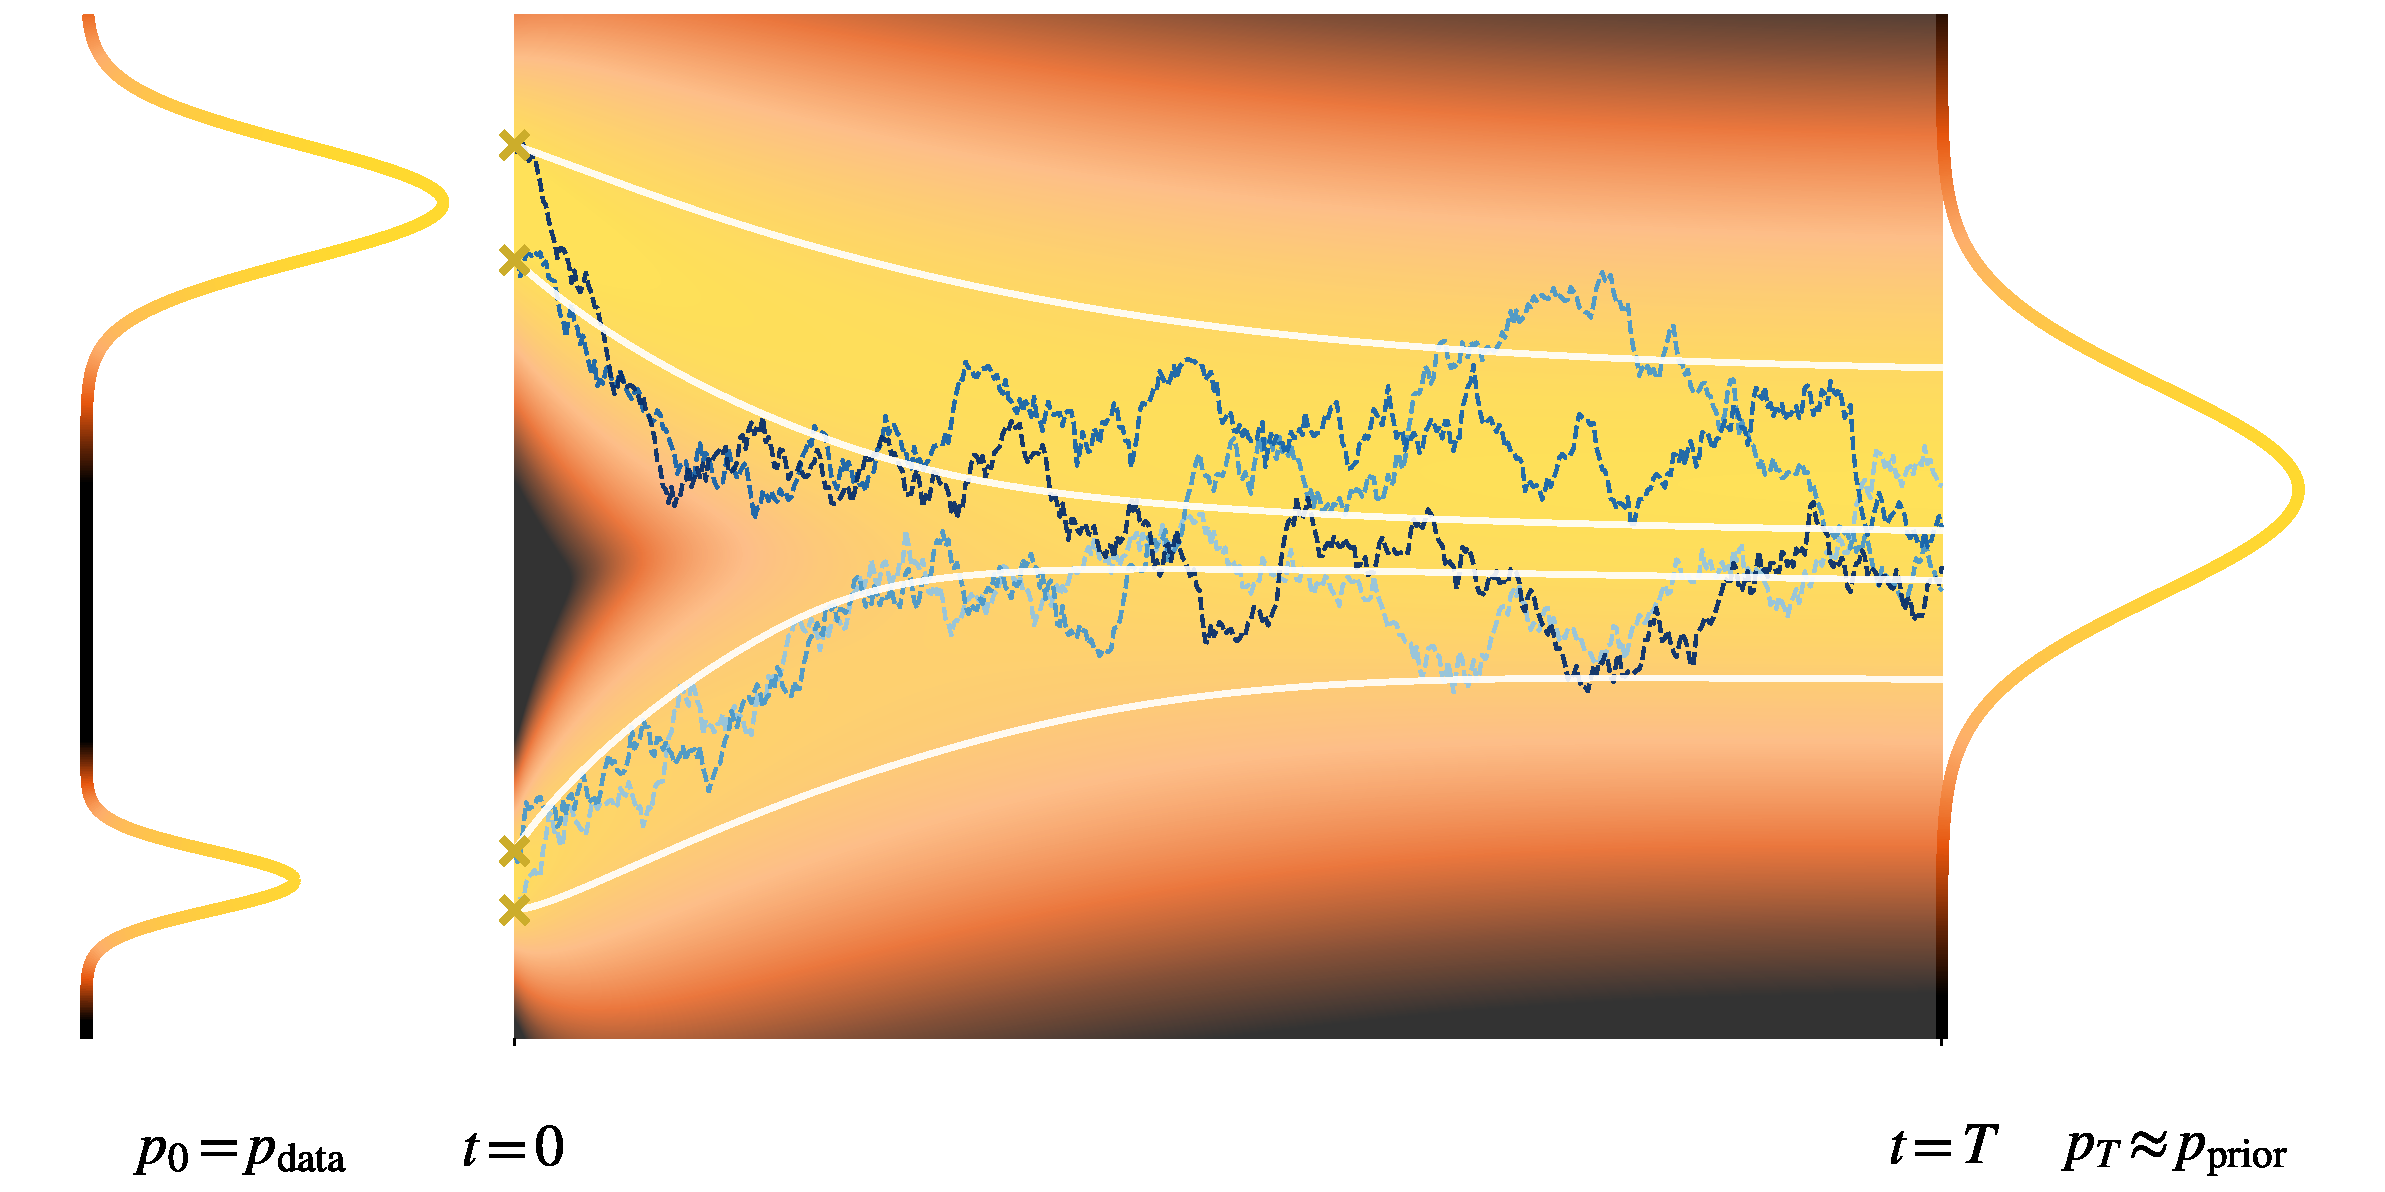
\includegraphics[width=\textwidth]{Images/PartB/forward_sde_ode_trajectories.pdf}
        \caption{\textbfs{（一维）扩散模型中前向过程的可视化。}该过程从复杂双峰数据分布（$p_0 = p_{\mathrm{data}}$）中采样得到的初始点（记为``$\times$''）出发，演化至简单的单峰高斯先验（$p_T \approx p_{\mathrm{prior}}$）。背景热力图展示了不断演化的边缘概率密度 $p_t$，它随时间逐渐变得平滑。图中展示了从 $t=0$ 到 $t=T$ 的样本轨迹，比较了随机前向 SDE 过程（蓝色路径）与其确定性对应物 PF-ODE（白色路径）。注意，PF-ODE 是密度的确定性传输映射，一般并不是从单点出发的样本路径的均值。 \figcredit{由作者绘制。}}

    \label{fig:sde-density-traj}
\end{figure}


借助这一表述，此前基于离散时间的方法，如 NCSN~\citep{song2019generative} 和 DDPM~\citep{sohl2015deep,ho2020denoising}，可以通过定义在区间 $[0, T]$ 上、由前向 SDE 控制的随机过程 $\rvx(t)$ 统一在\emph{连续时间}框架下：
\begin{mdframed}
\begin{equation}\label{eq:sde_forward}
    \diff\rvx(t) = \mathbf{f}(\rvx(t), t) \diff t + g(t) \diff\rvw(t), \quad \rvx(0) \sim p_{\mathrm{data}}.
\end{equation}
\end{mdframed}
这里，$\mathbf{f}(\cdot, t)\colon\mathbb{R}^D\to\mathbb{R}^D$ 是漂移项，$g(t) \in \mathbb{R}$ 是标量扩散系数，$\rvw(t)$ 表示标准 Wiener 过程。我们将其称为\emph{前向 SDE}，它描述了干净数据如何随时间被逐步扰动为噪声。

一旦指定了漂移项 $\mathbf{f}$ 和扩散系数 $g$，前向过程便完全确定，描述了数据变量如何通过注入高斯噪声而被逐步破坏。具体而言，它诱导出两族时间依赖的密度：
\paragraph{扰动核。}
条件分布律
\[
p_t(\rvx_t |\rvx_0)
\]
描述了一个干净数据样本 $ \rvx_0 \sim p_{\mathrm{data}} $ 如何在时刻 $t$ 演化为其含噪对应物 $\rvx_t$。一般而言，\Cref{eq:sde_forward} 中的漂移项 $\rvf(\rvx,t)$ 可以是 $\rvx$ 的任意函数，但一种常见且便于解析的选择是假设它为仿射形式：
\begin{equation}\label{eq:affine-drift}
    \rvf(\rvx,t) = f(t) \rvx, 
\end{equation}
其中 $f(t)$ 是 $t$ 的标量函数，通常取为非正。
在这一结构下，过程在每一时刻都保持高斯性，且条件分布存在通过求解相关的均值--方差 ODE~\citep{sarkka2019applied} 得到的闭式解（另见 \Cref{subsec:scoresde-perturbation-kernel}）。{特别地，
\[
p_t(\rvx_t |\rvx_0) = \mathcal{N} \big(\rvx_t; \rvm(t), P(t)\mathbf I_D\big),
\]
其中
\[
\rvm(t) = \exp \Big(\int_0^t f(u) \diff u\Big) \rvx_0,
\quad
P(t) = \int_0^t \exp \Big(2 \int_s^t f(u) \diff u\Big) g^2(s) \diff s,
\]
初始条件为 $\rvm(0)=\rvx_0$、$P(0)=0$。}

这一显式形式允许我们在给定 $\rvx_0$ 时直接采样 $\rvx_t$，而无需对 SDE 进行数值积分，因此被称为\emph{免仿真}（simulation-free）。NCSN 与 DDPM 都属于这种仿射漂移设定。

在下文中，我们针对任意漂移项 $\rvf(\rvx,t)$ 发展一般理论，但当闭式分析有用时，我们会回到仿射漂移的情形。



\paragraph{边缘密度。}
时间边缘密度 $ p_t(\rvx_t) $ 通过对扰动核积分得到：
\begin{equation}\label{eq:scoresde-oracle-marginal}
    p_t(\rvx_t) := \int p_t(\rvx_t|\rvx_0) p_{\mathrm{data}}(\rvx_0) \diff \rvx_0, \quad \text{with } p_0 = p_{\mathrm{data}}.
\end{equation}

{通过适当地选择系数 $f(t)$ 和 $g(t)$，前向过程逐步添加噪声，直到初始状态的影响被有效遗忘。当 $T$ 变大时，条件分布 $p_T(\mathbf{x}_T |\mathbf{x}_0)$ 不再依赖于 $\mathbf{x}_0$，因为其均值按如下方式演化
\[
\rvm(T) = \exp\!\Big(\int_0^T f(u)\diff u\Big) \mathbf{x}_0  \longrightarrow  \mathbf{0}, \quad \text{as } T\to\infty,
\]
只要 $f(u)$ 非正，从而使指数因子衰减。同时，方差增长并稳定以匹配所选的先验分布。}因此，边缘分布
\[
p_T(\mathbf{x}_T) = \int p_T(\mathbf{x}_T |\mathbf{x}_0) p_{\mathrm{data}}(\mathbf{x}_0)\diff\mathbf{x}_0,
\]
最初表示数据样本上的复杂混合，最终收敛到一个简单的先验 $p_{\mathrm{prior}}$，通常为高斯分布。在这一极限下，
\[
p_T(\mathbf{x}_T) \approx p_{\mathrm{prior}}(\mathbf{x}_T) 
\quad \text{and} \quad 
p_T(\mathbf{x}_T |\mathbf{x}_0) \approx p_{\mathrm{prior}}(\mathbf{x}_T),
\]
于是前向过程将任意数据分布映射为一个易于处理的先验，为反转与生成提供了便利的起点。




\subsection{用于生成的反向时间随机过程}\label{subsec:reverse-sde}



\begin{figure}[th!]
    \centering
    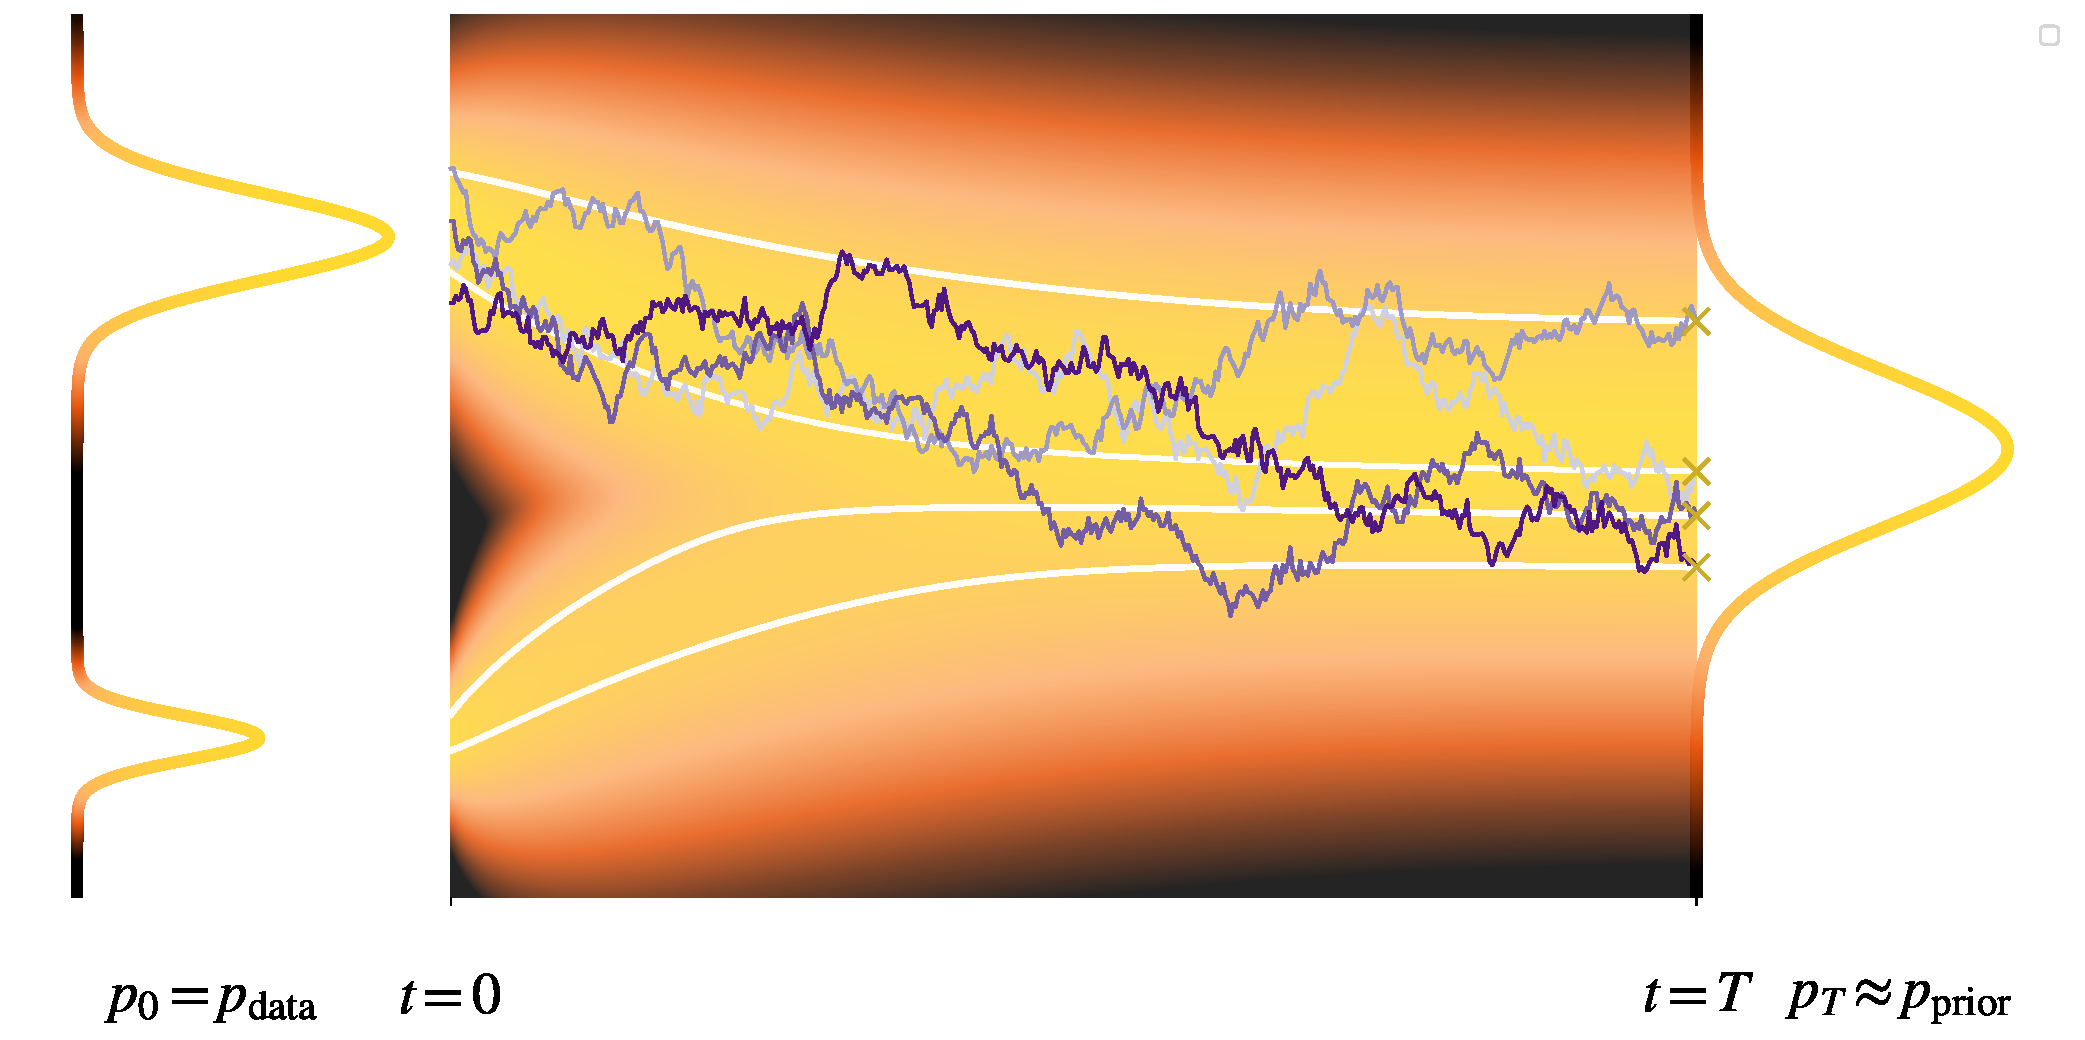
\includegraphics[width=\textwidth]{Images/PartB/reverse_sde_and_ode_trajectories.pdf}
    \caption{\textbfs{用于数据生成的反向时间随机过程的可视化。}
它从 $t=T$ 时由简单先验分布（$p_{\mathrm{prior}}$）中抽取的样本（记为``$\times$''）开始，使用反向 SDE 沿时间向后演化。
所得轨迹在 $t=0$ 处终止，并共同形成目标双峰数据分布（$p_0 = p_{\mathrm{data}}$）。背景热力图展示了概率密度如何从简单的高斯逐步转化为复杂的目标分布。
\figcredit{由作者绘制。}}
    \label{fig:sde-density-back-traj}
\end{figure}
直观上，从噪声生成数据可以通过对前向过程进行``反转''来实现：从先验分布中采样的随机点出发，沿时间向后演化以获得一个生成样本。对于确定性系统（即 ODE），这一想法自然成立。由于不涉及随机性，反转时间仅仅意味着沿与前向过程相同的路径、以相反方向追踪一个点的轨迹\footnote{在技术上，这对应于通过时间翻转替换 $t \leftrightarrow T - t$ 来求解 ODE。}。相比之下，SDE 在每个时间步都引入了随机性，这意味着单个点可以沿许多 plausible 的随机轨迹演化。因此，反转这类过程更为微妙\footnote{朴素地翻转时间并不能得到正确的反向过程。}。

虽然单条随机轨迹不可逆，但一个非凡的洞见是：这些轨迹上的分布是可以被反转的。这由 \citet{anderson1982reverse} 的一个基础结论形式化，它表明前向过程（\Cref{eq:sde_forward}）的时间反演过程 $\{ \bar{\rvx}(t) \}_{t \in [0, T]}$\footnote{我们使用``bar''记号以区分由前向时间 SDE 定义的前向过程 $\{ \rvx(t) \}_{t \in [0, T]}$ 与反向过程 $\{ \bar{\rvx}(t) \}_{t \in [0, T]}$。}本身受一个良定义的 SDE 所控制。这一反向时间过程从 $T$ 演化到 $0$，其动力学由下式给出：
\begin{mdframed}
\begin{align}\label{eq:sde_backward}
\begin{aligned}[t]
    \diff\bar{\rvx}(t) = \left[\mathbf{f}(\bar{\rvx}(t), t) {\color{orange} - g^2(t) \nabla_{\rvx} \log p_t(\bar{\rvx}(t))} \right] \diff t + g(t) \diff \bar{\rvw}(t), \\
    \hfill\bar{\rvx}(T) \sim p_{\mathrm{prior}} \approx p_T.
\end{aligned}
\end{align}
\end{mdframed}
这里，$\bar{\rvw}(t)$ 表示反向时间中的标准 Wiener 过程，定义为 $\bar{\rvw}(t) := \rvw(T - t) - \rvw(T)$。

为了建立对 \Cref{eq:sde_backward} 的直觉，我们在 \Cref{subsec:example-gaussian} 中给出了一个具体例子，采用高斯数据分布与线性--高斯动力学。这一设定在解析上易于处理：仅用基本微积分和线性代数即可直接推导出时间反演公式，而无需援引 \citet{anderson1982reverse} 的一般理论。
% \se{the gaussian linear dynamics system case could be instructive, you can work out the time reversal formula from basic math/linear algebra}

注意，随机性的存在（$g\neq 0$）引入了一个额外的修正项 $ -g^2(t) \nabla_{\rvx} \log p_t(\bar{\rvx}(t))$，它用于解释扩散的影响，并确保反向动力学正确地再现前向 SDE 所诱导的边缘分布演化（见 \Cref{subsec:fpe-sde-ode}）。

\paragraph{从概念上讲，反向过程为何有效？} \Cref{subsec:reverse-sde-reason} 通过将反向时间 SDE 与 DDPM 的变分框架相联系，给出了一个直观的推导（选读但富有洞见）。这里，我们为反向时间动力学如何从噪声中恢复结构化数据提供互补的直觉。


乍看之下，反向时间过程中存在布朗噪声似乎有些矛盾。如果前向扩散将数据扩散为越来越含噪的构型，那么如何通过反转这一过程（尤其是通过 $\bar{\rvw}(t)$ 引入额外随机性的过程）产生集中于数据流形附近的干净、结构化样本，并不清楚。关键在于反向时间 SDE 并不注入任意随机性。扩散项 $g(t)\diff\bar{\rvw}(t)$ 始终与分数驱动的漂移项 $- g^2(t)\nabla_{\rvx}\log p_t(\bar{\rvx}(t))$ 耦合在一起。这两项相互平衡：分数将轨迹引向更高密度的区域，而噪声则引入受控的随机性，使得在不压倒动力学的前提下进行探索。
% \se{refer to langevin?}

为更清楚地看到这一点，回到 \Cref{eq:continuous-langevin} 中的 Langevin 直觉。当 $f(t)\equiv 0$ 时，\Cref{eq:sde_backward} 写作
\[
\diff\bar{\rvx}(t)
= - g^2(t) \nabla_{\rvx}\log p_t\!\big(\bar{\rvx}(t)\big) \diff t
+ g(t)  \diff\bar{\rvw}(t).
\]
通过 $s:=T-t$（从而 $\diff t=-\diff s$）对时间进行前向重参数化，并在分布意义下将布朗运动重新记为 $\diff\bar{\rvw}(t)=-\diff\rvw_s$。记 $\bar{\rvx}_s:=\bar{\rvx}(T-s)$ 与 $\pi_s:=p_{T-s}$，得到
\begin{align*}
    \diff\bar{\rvx}_s
    &= g^2(T-s) \nabla\log \pi_s \big(\bar{\rvx}_s\big) \diff s
    + g(T-s) \diff\rvw_s
    \\&=
2\tau(s) \nabla\log \pi_s\!\big(\bar{\rvx}_s\big) \diff s
    + \sqrt{2\tau(s)} \diff\rvw_s,
    \quad
    \tau(s):=\tfrac{1}{2}g^2(T-s).
\end{align*}
这具有带随时间变化温度 $\tau(s)$、以不断演化的密度 $\pi_s$ 为目标的 Langevin 形式。根据 Tweedie 公式（\Cref{eq:tweedie}），分数方向 $\nabla\log \pi_s$ 在每个时间切片上都指向条件干净信号，因此漂移项持续地``拉回''去噪后的结构。

关键在于，$g(t)$ 沿反向轨迹是\emph{退火}的。起初（$s\approx 0$，即 $t\approx T$），$g(T-s)$ 通常较大，故注入的噪声较强，过程进行广泛的探索。随着 $s$ 增大，$g(T-s)$ 减小，随机项减弱，分数项占据主导，将样本拉入 $\pi_s$ 的高密度区域；到 $s=T$（即 $t=0$）时，轨迹集中于数据流形附近。



% \se{refer to langevin?}

\paragraph{反向时间 SDE 能力概述。}

% \se{i think it's worth saying that solving the reversesde generates sampling, and it's completely determined by the scores (so if we know them, we have all we need)}
令人着迷的是，时间依赖的分数函数
\[
\rvs(\rvx, t) := \nabla_{\rvx} \log p_t(\rvx)
\]
自然地出现在 \Cref{eq:sde_backward} 中。一旦指定了前向系数 $f(t)$ 和 $g(t)$，分数便是反向动力学中唯一剩下的未知量。这突出了它的核心作用：掌握了分数，反向过程便随之确定，而采样归结为用学得的分数对 \Cref{eq:sde_backward} 进行数值积分。

由于 oracle 分数一般没有闭式表达，我们采用 \Cref{ch:score-based} 的方法，训练一个神经网络 $\mathbf{s}_{\bm{\phi}}(\rvx, t)$ 通过分数匹配来逼近它；细节见 \Cref{subsec:sde-train}。将 \Cref{eq:sde_backward} 中的 $\rvs(\rvx, t)$ 替换为 $\mathbf{s}_{\bm{\phi}}(\rvx, t)$ 即可完全确定反向动力学。

生成对应于从 $t = T$ 出发、以 $\rvx_T \sim p_{\mathrm{prior}}$ 为初始值反向求解反向时间 SDE 至 $t = 0$。重要的是，\citet{anderson1982reverse} 证明了前向与反向过程的边缘密度重合，从而确保当 $p_{\mathrm{prior}} \approx p_T$ 时 $t=0$ 处的样本近似服从 $p_{\mathrm{data}}$。我们将在 \Cref{subsec:sde-sample} 中进一步探讨这一点。






\subsection{用于生成的确定性过程（概率流 ODE）}\label{subsec:pf-ode}
 尽管 \Cref{eq:sde_backward} 中的 SDE 引入了随机性并可能提高生成样本的多样性，但仍有一个问题：
\begin{question}
    是否必须使用 \Cref{eq:sde_backward} 中的 SDE 进行采样？
\end{question}

受 \citet{maoutsa2020interacting} 启发，\citet{song2020score} 还引入了一个确定性过程，即一个 ODE，它以与前向 SDE 相同的边缘分布演化样本。该过程 $\{\tilde\rvx(t)\}_{t\in[0,T]}$\footnote{我们使用波浪号以区分与前向及反向时间 SDE 相关联的过程。下文中，为简洁起见我们省略这一记号区分。}，称为\emph{概率流 ODE（PF-ODE）}，由下式给出：
\begin{mdframed}
    \begin{equation}\label{eq:prob_ode_gt}
    \frac{\diff}{\diff t}\tilde\rvx(t) = \mathbf{f}(\tilde\rvx(t), t) - \frac{1}{2} g^2(t) \nabla_{\rvx} \log p_t(\tilde\rvx(t)).
    \end{equation}
\end{mdframed}

与 SDE 的情形类似，可以用学得的逼近替换真实分数，并从 $t = T$ 到 $t = 0$ 积分反向时间 ODE 来生成样本。具体而言，生成样本（PF-ODE 在 $t=0$ 时的解）形如
\[
\tilde\rvx(T) + \int_{T}^{0} \Big[ \mathbf{f}(\tilde\rvx(\tau), \tau) - \frac{1}{2} g^2(\tau)  \nabla_{\rvx} \log p_\tau(\tilde\rvx(\tau)) \Big]   \diff \tau,
\]
其中初始条件 $\tilde\rvx(T) \sim p_{\mathrm{prior}}$。由于该积分没有闭式表达，实际生成依赖于数值求解器（例如 Euler 方法，见 \Cref{eq:euler-maruyama}）。

与反向时间 SDE 相比，PF-ODE 具有两大关键优势：
\begin{itemize}
    \item ODE 可以沿任一方向积分，既可从 $t=0$ 到 $t=T$，也可从 $t=T$ 到 $t=0$，且使用相同的方程表述，只要在所选端点处给定相应的初始条件即可。这种双向性与 SDE 形成对比，后者一般只允许前向时间积分。
    \item 它受益于为 ODE 开发的大量成熟、现成的数值求解器。
\end{itemize}


我们强调，PF-ODE 并非通过简单地移除 \Cref{eq:sde_backward} 中的扩散项得到；值得注意的是，其漂移项中 $\frac{1}{2}$ 这一因子具有原理性的来源。概括地说，\Cref{eq:prob_ode_gt} 来源于这样选择 ODE 的漂移项，使其演化保持与 \Cref{eq:sde_forward} 中前向 SDE 相同的边缘密度。保证这种边缘对齐的底层原理（即 Fokker-Planck 方程~\citep{oksendal2003stochastic}）将在下一节中详述。


\clearpage
\newpage



\section{前向/反向时间 SDE 与 PF-ODE 中的边缘分布匹配}\label{subsec:fpe-sde-ode}
\begin{figure}[th!]
% \vspace{-0.1cm}
    \centering
    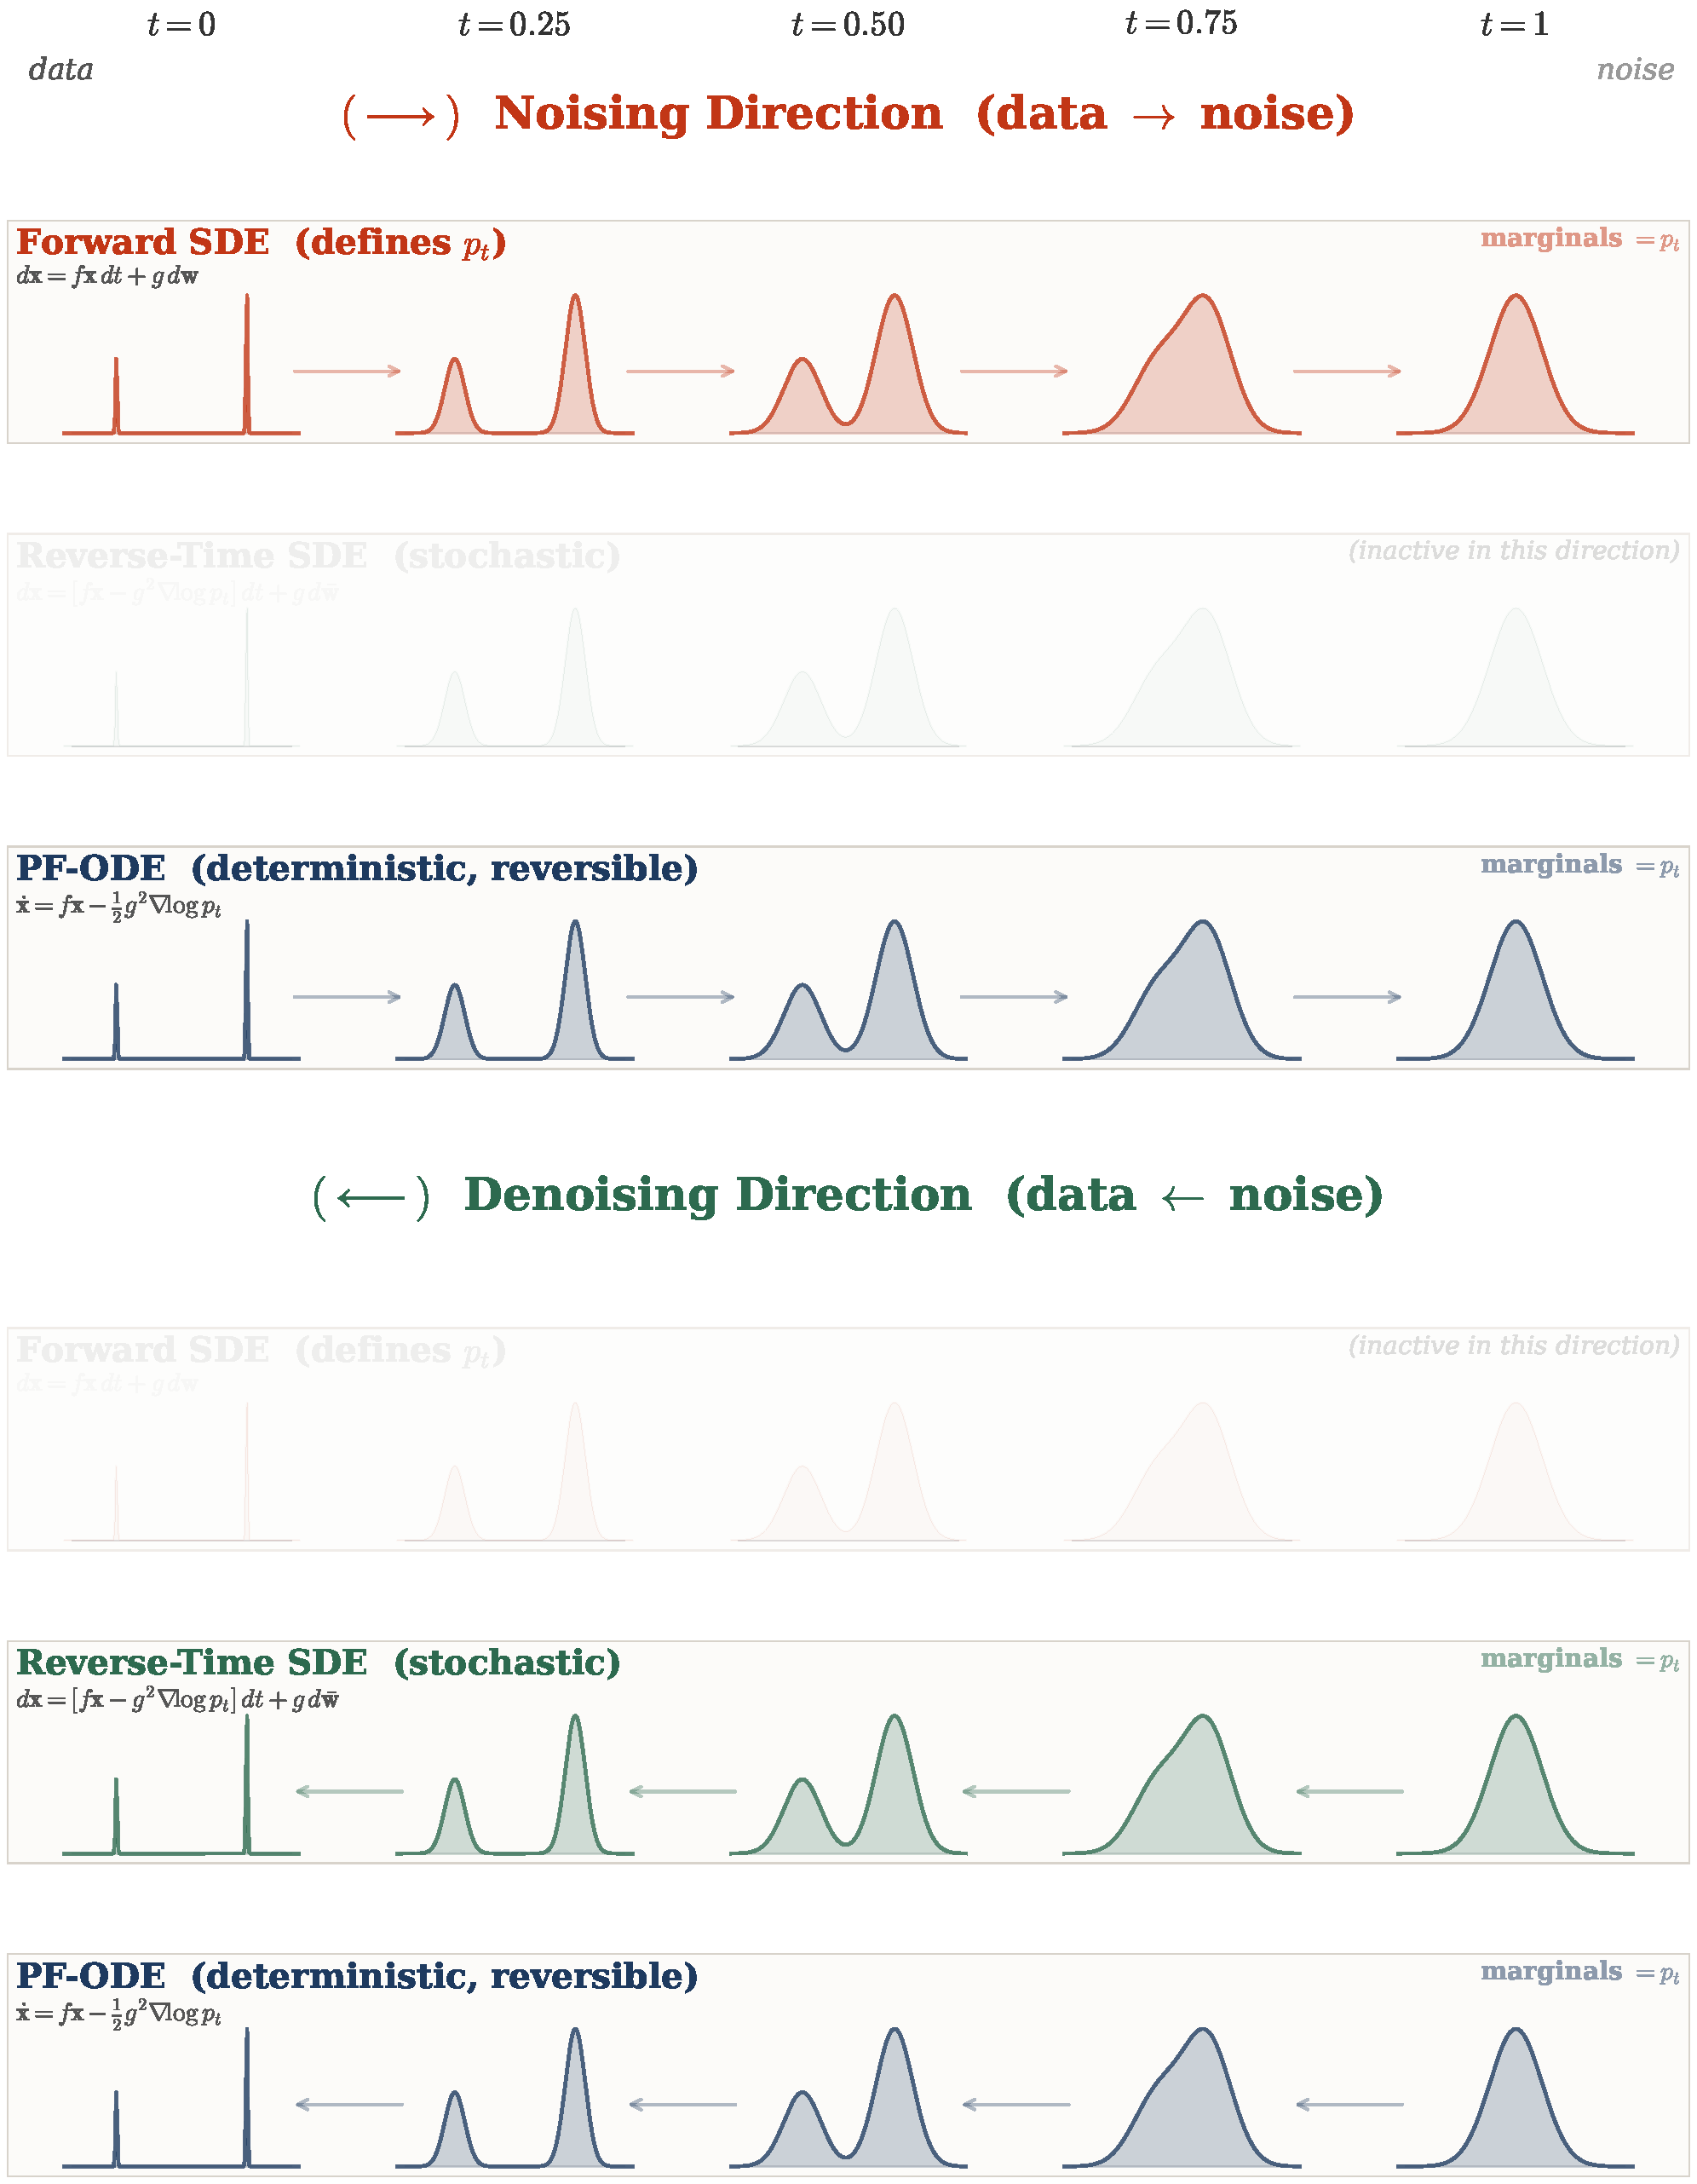
\includegraphics[width=\linewidth]{Images/PartB/score_sde_three_dynamics.pdf}
\caption{\textbfs{三种共享相同边缘分布 $p_t$ 的动力学。}
前向 SDE 作为锚定参考，通过将数据扩散为高斯先验来定义边缘分布 $p_t$。
反向时间 SDE 与 PF-ODE 产生相同的边缘分布，这由 Fokker-Planck 方程保证，同时通过分数 $\nabla \log p_t$ 沿去噪方向移动。
上方面板展示了加噪过程，由前向 SDE 给出，或在边缘层面等价地由沿时间正向运行的 PF-ODE 给出。
下方面板展示了去噪过程，由反向时间 SDE 或沿时间反向运行的 PF-ODE 给出。
PF-ODE 同时出现在两个面板中，因为它是确定性且时间可逆的。
\figcredit{由作者借助 AI 辅助编程绘制。}}
    \label{fig:score-sde-three-dynamics}
    \vspace{-2cm}
\end{figure}
本节中，我们将 \emph{Fokker-Planck 方程}作为支配扩散模型的核心原理加以介绍。它描述了概率密度在含噪动力学下如何演化，并在存在随机性时充当变量替换公式的自然类比（见 \Cref{app:continuity}）。从定义边缘分布 $p_t$ 的前向扩散过程出发，我们解释反向时间 SDE 与 PF-ODE 是如何被设计以再现相同的边缘分布族的。随后，我们通过一个高斯例子使这一原理具体化，在该例子中可以显式、直接地计算出反向时间 SDE 与 PF-ODE。




% \begin{center}
% % \vspace{-0.2cm}
% \includegraphics[width=0.67\linewidth]{Images/PartB/density_evolution_3d_orange.pdf}
%     \captionof{figure}{\textbfs{(2D) Temporal evolution of the marginal density $p_t$.} The forward SDE has $\mathbf{f} \equiv \mathbf{0}$ and $g(t) = \sqrt{2t}$ on $[0,T]$. It starts with $p_0 = p_{\mathrm{data}}$ a two-mode Gaussian mixture and ends at $p_T \approx p_{\mathrm{prior}} := \mathcal{N}(\mathbf{0}, T^2 \mathbf{I})$.  The temporal-spatial evolution of $p_t$ follows the Fokker-Planck equation.
% }
%     \label{fig:fpe-density}
% \end{center}
\subsection{确保边缘密度对齐的 Fokker-Planck 方程}
扩散模型中的一个核心概念是，\emph{不同的过程可以导致相同的边缘分布序列}（我们将在本小节后面加以说明）。
 目标是构造一个通过在时间上（尤其在 $t=0$ 处）对齐边缘分布从而将 $p_{\mathrm{prior}}$ 变换为 $p_{\mathrm{data}}$ 的过程。过程的具体形式是次要的，只要它是易于处理的并且允许高效采样。这自然引出一个根本问题：


\begin{question}
我们如何确保不同的过程产生相同的边缘分布？
\end{question}



回到我们的设定，一旦前向 SDE 被指定，它便定义了边缘密度从 $p_{\mathrm{data}}$ 到 $p_{\mathrm{prior}}$ 的演化。反向时间 SDE 与 PF-ODE 随后被构造出来，使其轨迹所产生的边缘分布与前向过程的边缘分布精确匹配。这种对应关系的关键在于 Fokker–Planck 方程，它支配着边缘密度在扩散过程下的演化。\Cref{fig:score-sde-three-dynamics} 给出了一个图示。下面的定理~\citep{anderson1982reverse,song2020score} 建立了这一联系的基础：
\thmp{Fokker–Planck 方程确保边缘分布对齐}{fpe}{设 $\{\rvx(t)\}_{t\in[0,T]}$ 随前向 SDE 演化
\[
\diff \rvx(t) = \rvf(\rvx(t),t)\diff t + g(t)\diff \rvw(t),
\]
初始条件为 $\rvx(0)\sim p_0 = p_{\mathrm{data}}$。则其边缘密度 $p_t$ 满足 Fokker–Planck 方程
\begin{align}\label{eq:fp_general}
\begin{aligned}
    \partial_t p_t(\rvx)
    &= - \nabla_{\rvx} \cdot\bigl[\rvf(\rvx,t) p_t(\rvx)\bigr]
       + \tfrac12 g^2(t) \Delta_{\rvx} p_t(\rvx)\\
    &= - \nabla_{\rvx} \cdot\bigl[\rvv(\rvx,t) p_t(\rvx)\bigr],
\end{aligned}
\end{align}
其中 $\Delta_{\rvx}$ 表示拉普拉斯算子，且
\[
 \rvv(\rvx,t)
 := \rvf(\rvx,t)
   -\tfrac12 g^2(t) \nabla_{\rvx}\log p_t(\rvx).
\]
那么，PF-ODE 与反向时间 SDE 都产生相同的边缘分布族 $\{p_t\}_{t \in [0, T]}$，其中后者沿反向时间演化：
\begin{enumerate}
  \item[\textup{(i)}] \emph{PF-ODE} $\{\tilde\rvx(t)\}_{t\in[0,T]}$
  \[
    \frac{\diff \tilde\rvx(t)}{\diff t}
    = \rvv(\tilde\rvx(t),t),
  \]
  若以 $\tilde\rvx(0)\sim p_0$ 为初始值并沿 $t$ 正向运行，或等价地以 $\tilde\rvx(T)\sim p_T$ 为初始值并沿 $t$ 反向运行，则对所有 $t\in[0,T]$ 都有边缘分布 $\tilde\rvx(t)\sim p_t$。

  \item[\textup{(ii)}] \emph{反向时间 SDE} $\{\bar\rvx(t)\}_{t\in[0,T]}$
  \[
    \diff \bar\rvx(t)
    = \bigl[\rvf(\bar\rvx(t),t) - g^2(t)\nabla_{\rvx}\log p_t(\bar\rvx(t))\bigr]\diff t
      + g(t)\diff \bar\rvw(t),
  \]
  其中 $\bar\rvx(0)\sim p_T$，$\bar\rvw(t)$ 为反向时间中的标准 Wiener 过程，其边缘分布为 $\bar\rvx(t)\sim p_{T-t}$。
\end{enumerate}
}{证明见 \Cref{app-sec:scoresde-fpe-proof}，而 \Cref{subsec:fpe-reason} 利用概率的边缘化技巧进一步提供了 Fokker–Planck 方程背后的直觉。
% \se{fix language}
}


% \rmkb{Anderson's reverse-time SDE theorem enables reversing diffusion processes under conditions where the evolved densities $p_t$ are \emph{absolutely continuous w.r.t. Lebesgue measure}, smooth, and positive for $t > 0$, even if the initial data distribution $p_0 = p_{\mathrm{data}}$ is singular (e.g., supported on a lower-dimensional manifold, violating absolute continuity at $t=0$). The forward diffusion induces absolute continuity and smoothness for $t > 0$, allowing the score function $\nabla \log p_t$ to be defined. However, in practice for both the reverse SDE and the PF-ODE, integration backward stops at a sufficiently small $\varepsilon > 0$ rather than $t=0$ to avoid divergence of the score near $t=0$, where $p_t$ approaches singularity under the manifold hypothesis; this ensures numerical stability and sample quality on $(\varepsilon, T]$.

% For simplicity, we still write $t=0$ in our discussion, without explicitly denoting $t=\varepsilon$ as the stopping time.}
% \se{not sure this remark is particularly insightful}


\paragraph{固定边缘分布下的多种条件分布。}
为理解 PF-ODE 如何将 $p_{\mathrm{data}}$ 沿时间向前传输（或等价地将 $p_{\mathrm{prior}}$ 沿时间反向传输），考虑\emph{流映射} $\bPsi_{s \to t}: \mathbb{R}^D \to \mathbb{R}^D$，其中 $\bPsi_{s \to t}(\rvx_s)$ 表示从时刻 $s$ 的 $\rvx_s$ 出发、PF-ODE 在时刻 $t$ 的解（对任意时刻 $s, t \in[0,T]$）。换言之，该映射取一个初始状态 $\rvx_s$ 并直接跳转到它在 $t$ 处的状态：
\begin{align}\label{eq:flow-map-def}
\bPsi_{s \to t}(\rvx_s) \coloneqq \rvx_s + \int_s^t \rvv(\rvx_\tau, \tau)\mathrm{d}\tau,
\end{align}
速度场为
\begin{align*}
\rvv(\rvx, \tau) := \rvf(\rvx, \tau) - \frac{1}{2} g^2(\tau)\nabla_{\rvx}\log p_\tau(\rvx).
\end{align*}
这里，积分刻画了沿 PF-ODE 轨迹 $\rvx_\tau$ 累积的净位移。在 $\rvv$ 满足温和光滑性假设的条件下，流映射 $\bPsi_{s \to t}: \mathbb{R}^D \to \mathbb{R}^D$ 是一个光滑双射\footnote{剧透：PF-ODE 的流映射 $\bPsi_{s\to t}$ 正是把 $p_s$ 搬运到 $p_t$ 的归一化流（NF）双射（详见 \Cref{sec:flow-based-method}）。区别在于 PF-ODE 固定了由 SDE 的 Fokker–Planck 动力学所决定的唯一向量场，而 NF（或连续时间 NF）对该场进行参数化，但依赖于相同的变量替换原理。
}.




对任意 $t\in[0,T]$，\emph{前推密度}定义为
\[
p_t^{\mathrm{fwd}}(\rvx_t) := \int \delta\bigl(\rvx_t - \bPsi_{0 \to t}(\rvx_0)\bigr)\, p_{\mathrm{data}}(\rvx_0) \,\diff \rvx_0,
\]
记为 $\bm{\Psi}_{0\to t} \sharp p_{\mathrm{data}}$，表示在 $\bm{\Psi}_{0\to t}$ 下时刻 $t$ 处的分布。定理~\ref{thm:fpe} 确保 $p_t^{\mathrm{fwd}} = p_t$，其中 $p_t$ 是前向 SDE 的边缘密度，从而将确定性的 PF-ODE 与随机核等同起来：
\[
p_t(\rvx_t) = \int p_t(\rvx_t |\rvx_0)\, p_{\mathrm{data}}(\rvx_0)\,\diff \rvx_0
= \int \delta\bigl(\rvx_t - \bm{\Psi}_{0\to t}(\rvx_0)\bigr)\, p_{\mathrm{data}}(\rvx_0)\,\diff \rvx_0.
\]

这意味着存在无穷多个条件分布 $Q_t(\rvx_t |\rvx_0)$ 都产生相同的 $p_t(\rvx_t)$，例如：
\begin{itemize}
  \item \textbfs{随机（免仿真）：}$Q_t(\rvx_t |\rvx_0) = p_t(\rvx_t |\rvx_0)$，
  \item \textbfs{确定性（需要求解 ODE）：}$Q_t(\rvx_t |\rvx_0) = \delta\bigl(\rvx_t - \bm{\Psi}_{0\to t}(\rvx_0)\bigr)$，
  \item \textbfs{混合：}$Q_t(\rvx_t |\rvx_0) = \lambda p_t(\rvx_t |\rvx_0) + (1-\lambda)\delta\bigl(\rvx_t - \bm{\Psi}_{0\to t}(\rvx_0)\bigr)$，$\lambda\in[0,1]$。
\end{itemize}
$Q_t(\rvx_t |\rvx_0)$ 的这种非唯一性源于如下事实：边缘约束并不能唯一地确定条件分布。这一概念将在 \Cref{subsec:fm-framework} 和 \Cref{subsec:ddim} 中再次出现。特别地，存在整整一族与同一边缘分布 $p_t$ 相一致的反向时间 SDE。

\msg{观察}{匹配给定的边缘密度}{
多个过程可以产生相同的边缘密度序列；真正重要的是满足 Fokker–Planck 方程。这一基本洞见为我们设计从 $ p_{\mathrm{prior}} $ 转移到 $ p_{\mathrm{data}} $（或反之）的生成过程提供了极大的灵活性。
}
Fokker–Planck 方程是扩散模型的核心，它根植于概率密度的基本\emph{变量替换公式}（系统论述见 \Cref{app:continuity}）。这一原理绝非次要的技术细节，它在我们的整个论述中反复出现，最显著的是在 \Cref{sec:flow-matching-framework}。
% , and reveals deep structural connections among seemingly different formulations.
% \se{either cut or provide more detail here on this connection}



\subsection{一个可计算的例子：高斯动力学的演化}\label{subsec:example-gaussian}
当 $p_{\mathrm{data}}$ 是正态分布（或高斯混合）时，分数函数具有闭式表达。
这使它成为建立扩散过程直觉的理想设定：我们只需用到基本微积分，就能显式地推导出反向时间 SDE 与 PF-ODE，而无需诉诸高级数学工具。
在本小节中，我们说明这些方程在这样易于处理的情形下是如何表现的。



\paragraph{高斯情形下反向时间 SDE 的精确计算。}
 当 $p_{\mathrm{data}}$ 为高斯时，\Cref{eq:sde_backward} 中的公式可以直接推导，而无需依赖 \citet{anderson1982reverse} 的一般理论与证明。为阐明核心思想，我们考虑一维情形；向高维的推广同理。



从前向 SDE 出发
\[
\diff x(t)  =  f(t)  x(t)  \diff t  +  g(t)  \diff w_t,
\]
取一个大小为 $\Delta t>0$ 的小 Euler 步：
\[
x_{t+\Delta t}  =  a  x_t  +  r  \epsilon,
\]
其中 $a:=1+f(t)\Delta t$，$r:=g(t)\sqrt{\Delta t}$，$ \epsilon\sim\mathcal N(0,1)$。等价地，前向单步转移核为高斯：
\[
x_{t+\Delta t}   |   x_t  \sim  \mathcal N\!\big(a  x_t,   r^2\big).
\]
由于假设 $p_{\mathrm{data}}$ 为高斯，时刻 $t$ 处的当前边缘分布也是高斯，形如：
\[
x_t \sim \mathcal N(m_t,   s_t^2),
\]
其中 $m_t$ 和 $s_t$ 为某标量。于是条件化就归结为两个高斯相乘并重新归一化。这使得代数运算保持初等。

由贝叶斯法则，条件密度（忽略常数）是先验与转移核的乘积：
\begin{align*}
    p(x_t   |   x_{t+\Delta t})  &\propto p(x_{t+\Delta t} | x_t   ) p_t(\rvx_t) \\&\propto
\exp\Big(-\frac{(x_t-m_t)^2}{2s_t^2}\Big)  
\exp\Big(-\frac{(x_{t+\Delta t}-a  x_t)^2}{2r^2}\Big).
\end{align*}
其指数是关于 $x_t$ 的二次型。展开两个平方并合并同类项，可以清楚地看到哪些系数起作用：
\[
-2\log p(x_t   |   x_{t+\Delta t})
 = 
A  x_t^2  -  2 B  x_t  +  \text{const},
\]
其中
\[
A:=\frac{1}{s_t^2}+\frac{a^2}{r^2},\quad
B:=\frac{m_t}{s_t^2}+\frac{a  x_{t+\Delta t}}{r^2}.
\]
这里 $A$ 是精度之和（先验精度加上通过 $a$ 传输过来的转移核精度），而 $B$ 是目标值的相应精度加权和。有了这些，配方便可一行写出后验：
\[
A x_t^2 - 2 B x_t
  =  
A\Big(x_t-\frac{B}{A}\Big)^2  -  \frac{B^2}{A},
\]
故条件分布是方差为 $1/A$、均值为 $B/A$ 的高斯：
\[
\Var(x_t   |   x_{t+\Delta t})   =   \frac{1}{\frac{1}{s_t^2}+\frac{a^2}{r^2}},
\qquad
\mathbb E[x_t   |   x_{t+\Delta t}]   =  
\frac{\frac{m_t}{s_t^2}+\frac{a  x_{t+\Delta t}}{r^2}}{\frac{1}{s_t^2}+\frac{a^2}{r^2}}.
\]
这些闭式已经刻画了任意小 $\Delta t$ 的反向转移。为读出一个反向时间 SDE，我们现在对小 $\Delta t$ 进行展开。

利用 $a=1+f(t)\Delta t$ 与 $r^2=g^2(t)\Delta t$。当 $\Delta t\to 0$ 时，$\frac{a^2}{r^2}\sim \frac{1}{g^2(t)\Delta t}$ 主导精度，故方差变为
\[
\Var(x_t   |   x_{t+\Delta t})
= \left(\frac{1}{s_t^2}+\frac{a^2}{r^2}\right)^{-1}
= g^2(t)  \Delta t  +  \mathcal{O}(\Delta t^2),
\]
这告诉我们反向步具有与前向步相同的扩散尺度 $g(t)$。对于均值，将比值 $B/A$ 展开到一阶：
\[
\mathbb E[x_t   |   x_{t+\Delta t}]
  =  x_{t+\Delta t}
 +  \Delta t\left[
-\left(f(t)+\frac{g^2(t)}{s_t^2}\right)  x_{t+\Delta t}
 +  \frac{g^2(t)}{s_t^2}  m_t
\right]  +  \mathcal{O}(\Delta t^2).
\]

将均值与方差合在一起，得到单步反向转移核
\[
x_t    |    x_{t+\Delta t}
 \sim 
\mathcal N\!\left(
x_{t+\Delta t} + \Delta t\!\left[-\left(f+\frac{g^2}{s_t^2}\right)  x_{t+\Delta t} + \frac{g^2}{s_t^2}  m_t\right],
 g^2  \Delta t\right)
 +  \mathcal{O}(\Delta t^2).
\]
这可以识别为从 $t+\Delta t$ 反向运行到 $t$ 的 Euler–Maruyama 更新：
\[
x_t - x_{t+\Delta t}
= \Delta t\!\left[-\left(f+\frac{g^2}{s_t^2}\right) x_{t+\Delta t} + \frac{g^2}{s_t^2} m_t\right]
+ g\sqrt{\Delta t} \epsilon + O(\Delta t^2).
\]
令 $\Delta t\to 0$ 得到原时钟上的 SDE（时间沿路径递减）
\[
\diff x(t)
= \Big[-\Big(f(t)+\frac{g^2(t)}{s_t^2}\Big) x(t) + \frac{g^2(t)}{s_t^2} m_t\Big]\diff t
+ g(t) \diff \bar w_t .
\]
这一漂移项可以用分数写出，因为对于高斯边缘 $p_t=\mathcal N(m_t,s_t^2)$，
\[
\partial_x \log p_t(x) = -\frac{x-m_t}{s_t^2}
 \Longrightarrow 
-\Big(f+\frac{g^2}{s_t^2}\Big) x + \frac{g^2}{s_t^2} m_t
= -f x + g^2 \partial_x\log p_t(x).
\]
为表达传统的\emph{按 $t$ 前向}的反向时间参数化，定义反向过程 $\bar x(t):=x(T-t)$（从而我们现在沿 $t$ 前向演化）。时间翻转将漂移项变为
\[
\diff \bar x(t)
= \Big[ f(t) \bar x(t)  -  g^2(t) \partial_x \log p_t(\bar x(t)) \Big]\diff t
+ g(t)\diff \bar w_t,
\]
其中 $\bar x(T)\sim p_{\mathrm{prior}}\approx p_T$。这正是传统的反向时间 SDE。写成向量形式后，它与一般的 \Cref{eq:sde_backward} 一致，只是以 $\nabla_{\rvx}\log p_t$ 代替一维导数。

\paragraph{高斯情形下 PF-ODE 的精确计算。}
当数据分布假设为高斯时，我们也可以直接推导 PF-ODE 公式，避免诸如 Fokker–Planck 方程之类的重型工具。最终，我们将看到 PF-ODE 的边缘密度与前向 SDE 和反向时间 SDE 的边缘密度重合，从而对 \Cref{subsec:fpe-sde-ode} 中将讨论的 Fokker–Planck 理论给出构造性验证。


假设在时刻 $t$ 有 $x_t\sim\mathcal N(m_t,s_t^2)$。一个大小为 $\Delta t$ 的小确定性步可写成一个光滑映射
\[
x_{t+\Delta t}=\Phi_{t,\Delta t}(x_t)
= x_t + \Delta t v_t(x_t) + \mathcal{O}(\Delta t^2),
\]
它不过是关于 $\Delta t$ 的一阶泰勒展开。我们的目标是看清楚 $v_t$ 必须取何种形式，才能在输入为高斯时输出仍保持高斯。

为此，在当前均值 $m_t$ 处展开 $v_t$：
\[
v_t(x)=v_t(m_t)+v_t'(m_t)(x-m_t)+\tfrac12 v_t''(m_t)(x-m_t)^2+\cdots.
\]
令 $y:=x_t-m_t$，则 $y\sim\mathcal N(0,s_t^2)$。接着，将输出中心化（减去其均值，精确到 $\Delta t$ 的一阶）：
\[
z:=x_{t+\Delta t}-\mathbb E[x_{t+\Delta t}]
= y + \Delta t\!\left(v_t'(m_t) y+\tfrac12 v_t''(m_t) (y^2-s_t^2)\right)+\mathcal{O}(\Delta t^2).
\]
此时，回忆高斯的偏度为零；换言之，其三阶中心矩为零。因此，将 $\mathbb E[z^3]$ 计算到一阶并利用
$\mathbb E[y]=0$，$\mathbb E[y^2]=s_t^2$，$\mathbb E[y^3]=0$，$\mathbb E[y^4]=3s_t^4$，
得到
\[
\mathbb E[z^3]
= 3 \Delta t\cdot \tfrac12 v_t''(m_t) \big(\mathbb E[y^4]-s_t^2\mathbb E[y^2]\big)+\mathcal{O}(\Delta t^2)
= 3 \Delta t v_t''(m_t) s_t^4+\mathcal{O}(\Delta t^2).
\]
要使输出对所有小的 $\Delta t$ 都保持高斯，这个量必须在 $\Delta t$ 阶上消失，这迫使 $v_t''(m_t)=0$。对更高阶导数重复同样论证，也会排除更高次项。因此，$v_t$ 必须是线性的再加一个平移：
\[
v_t(x)=a_t x+b_t.
\]
将其代回该步，得到
\[
x_{t+\Delta t}=(1+\alpha_t \Delta t) x_t+\beta_t \Delta t+\mathcal{O}(\Delta t^2),
\qquad
\alpha_t:=a_t,\ \ \beta_t:=b_t.
\]

现在将 $x_t\sim\mathcal N(m_t,s_t^2)$ 通过这一映射，并跟踪均值和方差到一阶：
\begin{align*}
\mathbb E[x_{t+\Delta t}]
&= m_t+\Delta t(\alpha_t m_t+\beta_t)+\mathcal{O}(\Delta t^2),
\\
\Var(x_{t+\Delta t})
&= s_t^2+\Delta t (2\alpha_t s_t^2)+\mathcal{O}(\Delta t^2).
\end{align*}
另一方面，前向 SDE $\diff x=f(t) x \diff t+g(t) \diff w_t$ 具有初等的矩公式（见 \Cref{eq:mean-var-evolution}）：
\[
m_t' = f(t) m_t,
\qquad
(s_t^2)' = 2 f(t) s_t^2 + g^2(t).
\]
匹配 $\Delta t$ 的系数，得到
\[
\alpha_t = f(t)+\frac{g^2(t)}{2 s_t^2},
\qquad
\beta_t = - \frac{g^2(t)}{2 s_t^2} m_t.
\]

在这些选择下，该步变为
\[
x_{t+\Delta t}
= x_t + \Delta t\!\left[\Big(f(t)+\frac{g^2(t)}{2s_t^2}\Big)x_t
-\frac{g^2(t)}{2s_t^2} m_t\right]+\mathcal{O}(\Delta t^2).
\]
由于对于高斯 $p_t=\mathcal N(m_t,s_t^2)$ 有 $\partial_x\log p_t(x)=-(x-m_t)/s_t^2$，我们可以将方括号改写为
$f(t) x_t - \tfrac12 g^2(t) \partial_x\log p_t(x_t)$。
因此，
\[
x_{t+\Delta t}
= x_t + \Delta t\Big[f(t) x_t - \tfrac12 g^2(t) \partial_x\log p_t(x_t)\Big] + \mathcal{O}(\Delta t^2).
\]
最后，除以 $\Delta t$ 并令 $\Delta t\to 0$，得到 PF-ODE
\[
x'(t)  =  f(t) x(t)  -  \tfrac12 g^2(t) \partial_x\log p_t\!\big(x(t)\big).
\]

为看到为何这一 ODE 具有与前向 SDE（以及反向时间 SDE）相同的边缘分布，注意上面的漂移项是线性的再加上一个平移。因此 $x(t)$ 仿射地依赖于 $x(0)$，而仿射映射将高斯映为高斯。此外，沿该 ODE 的均值 $m_t$ 和方差 $s_t^2$ 满足与前向 SDE 完全相同的两个标量 ODE（由我们的匹配得到），且具有相同的初始值。因此，在每个时刻 $t$ 都有 $p_t=\mathcal N(m_t,s_t^2)$ 对两种演化都相同.




\clearpage
\newpage



\section{Score SDE：其训练与采样}\label{sec:scoresde-training-sampling}

\subsection{训练}\label{subsec:sde-train}
秉承 \Cref{ch:score-based} 中的思想，我们用一个时间条件化的神经网络来逼近 oracle 分数 $\nabla_{\rvx} \log p_t(\rvx)$
\[
\mathbf{s}_{\bm{\phi}} = \mathbf{s}_{\bm{\phi}}(\rvx, t)
\]
覆盖所有 $t\in[0,T]$，其方式是最小化如 \Cref{eq:sm} 的分数匹配目标：
\begin{equation*}
\mathcal{L}_{\text{SM}}(\bm{\phi}; \omega(\cdot)) := \frac{1}{2} \mathbb{E}_{t\sim p_{\text{time}}}  \mathbb{E}_{\rvx_t \sim p_t}\left[\omega(t) \left\|\mathbf{s}_{\bm{\phi}}(\rvx_t, t) - \nabla_{\rvx} \log p_t(\rvx_t)\right\|_2^2\right],
\end{equation*}
其中 $p_{\text{time}}$ 是某个时间分布（例如 $[0,T]$ 上的均匀分布），$\omega(\cdot)$ 是一个时间加权函数。

\begin{figure}[th!]
    \centering
    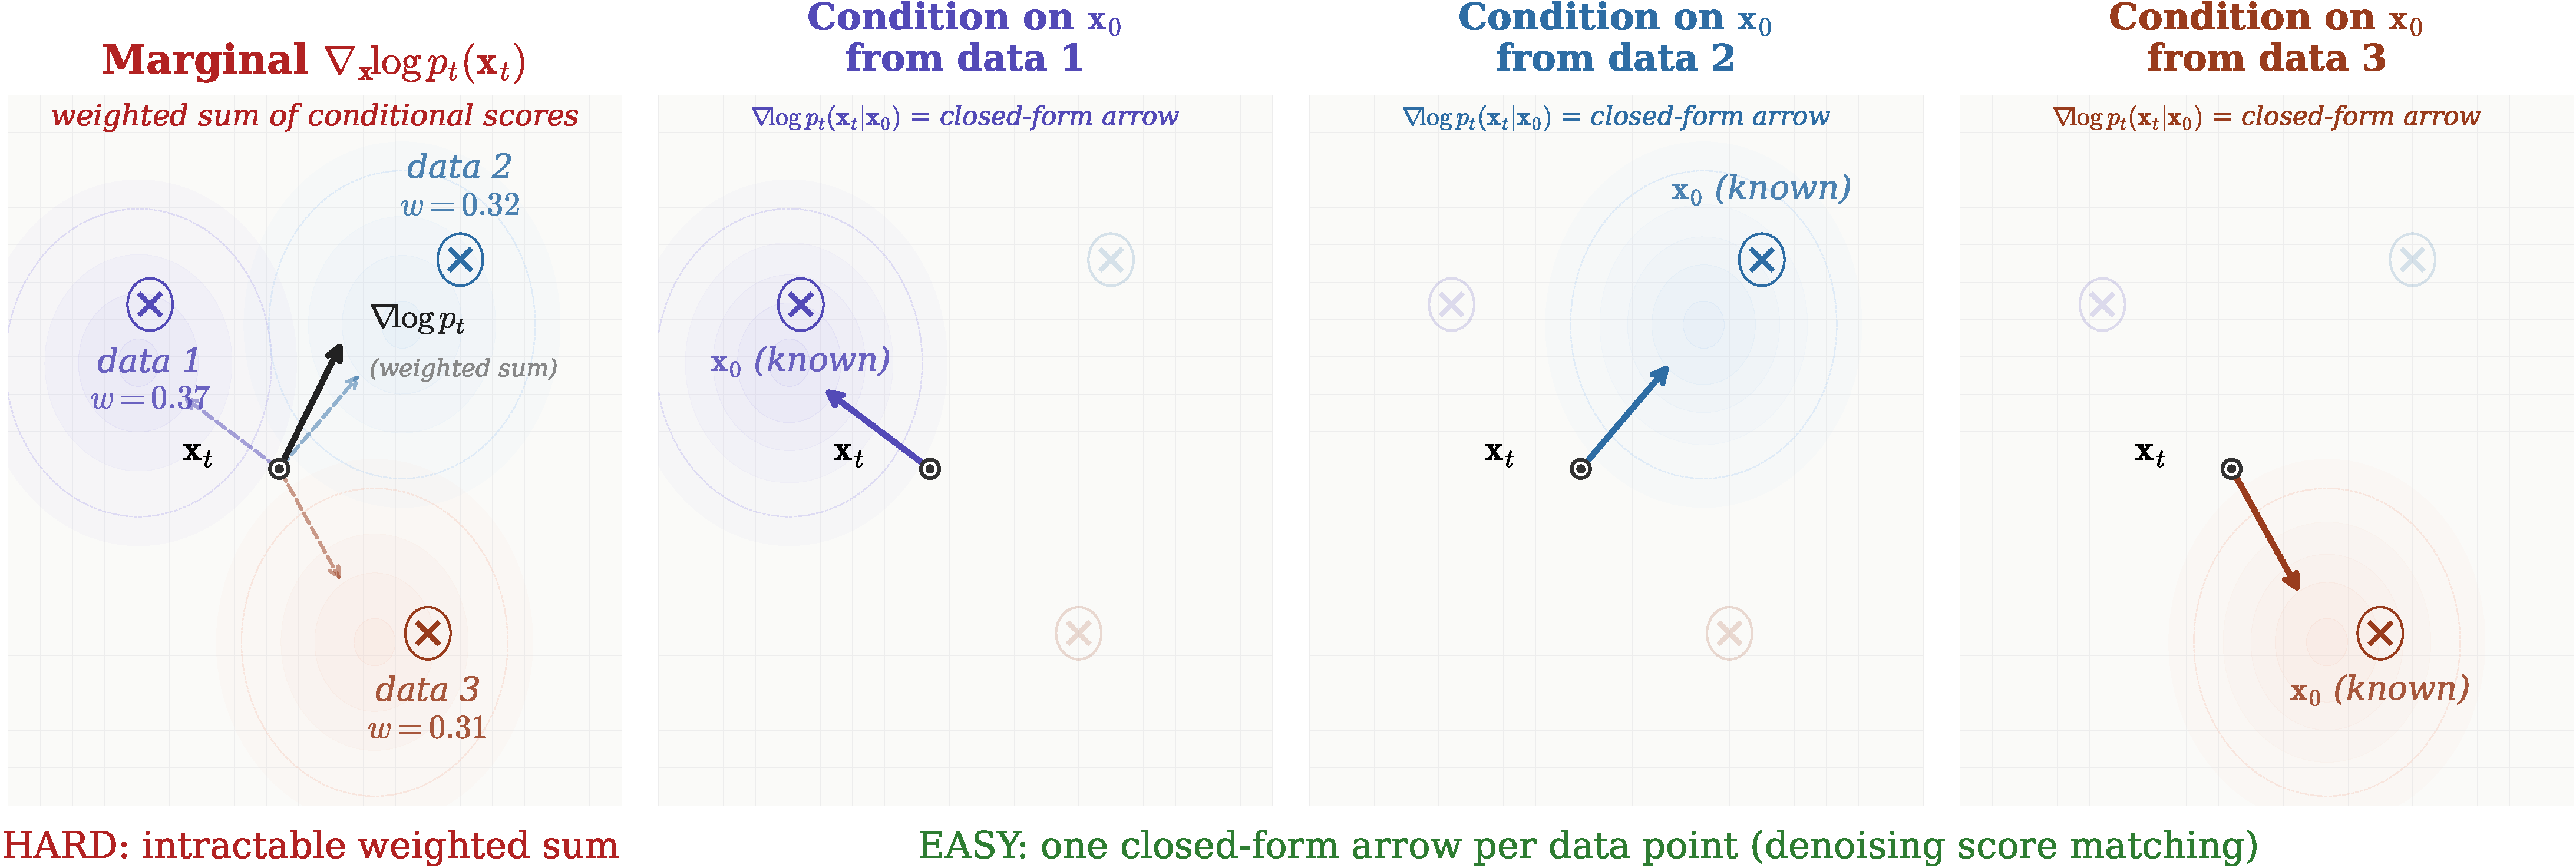
\includegraphics[width=\linewidth]{Images/PartB/denoising_score_matching.pdf}
    \caption{\textbfs{去噪分数匹配技巧的示意图。}
边缘分数 $\nabla_{\rvx_t}\log p_t(\rvx_t)$ 通常是所有可能的干净样本 $\rvx_0$ 上条件分数的难以处理的加权平均，其权重由在含噪观测 $\rvx_t$ 条件下 $\rvx_0$ 的后验分布给出。
然而，对于每个固定的 $\rvx_0$，条件分数 $\nabla_{\rvx_t}\log p_t(\rvx_t|\rvx_0)$ 具有闭式表达。
去噪分数匹配将这一困难的边缘估计问题转化为容易的逐样本回归问题。
\figcredit{由作者借助 AI 辅助编程绘制。}}
    \label{fig:score-and-denoising-score}
\end{figure}


为避免依赖难以处理的 oracle 分数 $\nabla_{\rvx} \log p_t(\rvx)$，我们采用 \Cref{eq:dsm-loss} 中的 DSM 损失。以数据点 $\rvx_0$ 为条件，该方法允许通过 \Cref{eq:score-gaussian-formula} 使用解析上易于处理的分数 $\nabla_{\rvx_t} \log p_t(\rvx_t|\rvx_0)$，具体例子见 \Cref{sec:instances}。具体而言，我们采用如下损失函数：
\begin{mdframed}
    \begin{equation}\label{eq:conti-dsm_loss-real}
\begin{aligned}
     &\mathcal{L}_{\text{DSM}}(\bm{\phi}; \omega(\cdot)) := \\
     &\frac{1}{2} \mathbb{E}_{t}  \mathbb{E}_{\rvx_0} \mathbb{E}_{ p_t(\rvx_t|\rvx_0)} \Big[\omega(t)\norm{\mathbf{s}_{\bm{\phi}}(\rvx_t, t) - \nabla_{\rvx_t} \log p_t(\rvx_t|\rvx_0)}_2^2 \Big],
\end{aligned}
\end{equation}
\end{mdframed}
其中 $\rvx_0 \sim p_{\mathrm{data}}$。\Cref{eq:conti-dsm_loss-real} 可以理解为 \Cref{eq:nscn} 的连续时间对应物，离散情形中的求和被积分替代。


类似定理~\ref{thm:sm-dsm} 中的结论，\Cref{eq:conti-dsm_loss-real} 的最小化子唯一确定如下：

\proppp{DSM 的最小化子}{dsm-minimizer}{
最小化子 $\mathbf{s}^*$ 满足
\begin{align}\label{eq:optimal-score}
\begin{aligned}
    \mathbf{s}^*(\rvx_t, t) 
    = \mathbb{E}_{\rvx_0 \sim p(\rvx_0 | \rvx_t)} \big[ \nabla_{\rvx_t} \log p_t(\rvx_t | \rvx_0) \big]= \nabla_{\rvx_t} \log p_t(\rvx_t),
\end{aligned}
\end{align}
对几乎所有的 $\rvx_t \sim p_t$ 与 $t \in [0,T]$ 成立。}{ 
DSM 目标可以理解为一个最小二乘误差问题。具体而言，在每个时刻 $t$，最优分数函数由对数条件密度梯度的条件期望给出，而根据贝叶斯法则，这等价于对数边缘密度的梯度。详细证明见附录~\ref{app-sec:min-dsm}。
}


\subsection{采样与推断}\label{subsec:sde-sample}
\begin{figure}[th!]
    \centering
    \vspace{-0.8cm}
    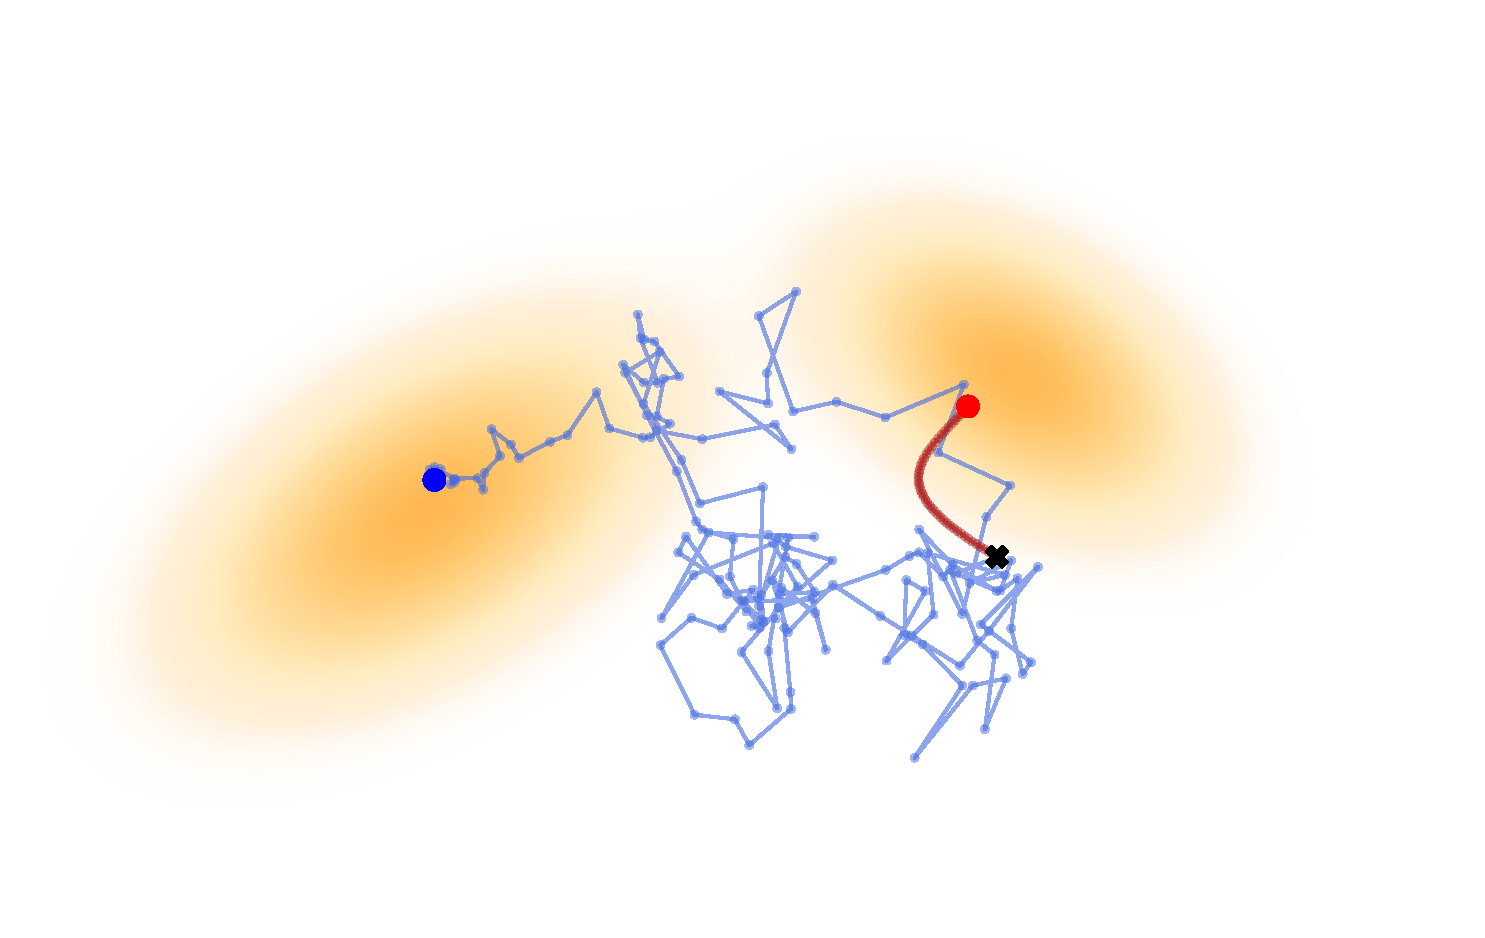
\includegraphics[width=\linewidth]{Images/PartB/sde_ode_trajectories.pdf}
    \vspace{-0.6cm}
    \caption{\textbfs{（二维）从 Score SDE 采样的示意图。}前向 SDE 设计为 $\diff\rvx(t)=\sqrt{2t}\diff\rvw(t)$，其漂移项 $\mathbf{f}\equiv\mathbf{0}$、扩散系数 $g(t)=\sqrt{2t}$（在 $[0,T]$ 上），将双峰高斯混合 $p_0=p_{\mathrm{data}}$ 演化为 $p_T\approx p_{\mathrm{prior}}:=\mathcal{N}(\mathbf{0},T^2\mathbf{I})$。图中展示了反向时间 SDE（蓝色；由 \Cref{eq:euler-maruyama} 求解）和 PF-ODE（红色；由 \Cref{eq:euler-ode} 求解）的采样轨迹。从随机点 $\rvx_T\sim p_{\mathrm{prior}}$（深色``$\times$''）出发，两条轨迹都随着 $t\to 0$ 朝 $p_{\mathrm{data}}$ 的支撑集移动。
    \figcredit{由作者绘制。}}
    \label{fig:sde_ode_trajectories}
\end{figure}


在学得
\[
\mathbf{s}_{\bm{\phi}^\times} := \mathbf{s}_{\bm{\phi}^\times}(\rvx, t) \approx \nabla_{\rvx} \log p_t(\rvx),
\]
之后，我们将反向时间 SDE（\Cref{eq:sde_backward}）与 PF-ODE（\Cref{eq:prob_ode_gt}）中难以处理的 oracle 分数 $\nabla_{\rvx} \log p_t(\rvx)$ 替换为学得的代理 $\mathbf{s}_{\bm{\phi}^\times}(\rvx, t)$。这一替换使得通过 SDE 或 ODE 进行易于处理的推断成为可能。为清楚起见，我们将所得过程分别记为 $\rvx^{\mathrm{SDE}}_{\bm{\phi}^\times}(t)$ 和 $\rvx^{\mathrm{ODE}}_{\bm{\phi}^\times}(t)$，但在后续章节中将省略这一区分。\footnote{这是为了在本小节之后简化记号。}

\paragraph{经验反向时间 SDE。}
通过在 \Cref{eq:sde_backward} 中用训练好的分数模型 $\mathbf{s}_{\bm{\phi}^\times}$ 替换真实分数，我们得到用于生成的参数化反向时间 SDE：
\begin{equation}\label{eq:sde_backward_sub}
    \diff \rvx^{\mathrm{SDE}}_{\bm{\phi}^\times}(t) = \left[\mathbf{f}\left(\rvx^{\mathrm{SDE}}_{\bm{\phi}^\times}(t), t\right) - g^2(t) \mathbf{s}_{\bm{\phi}^\times}\left(\rvx^{\mathrm{SDE}}_{\bm{\phi}^\times}(t), t\right) \right] \diff t + g(t) \diff \bar{\rvw}(t).
\end{equation}
为生成一个样本，我们首先从先验分布 $p_{\mathrm{prior}}$ 中抽取一个初始值 $\rvx_T$，然后从 $t=T$ 到 $t=0$ 反向数值求解 \Cref{eq:sde_backward_sub}。一种标准的数值求解器是 Euler–Maruyama 方法，它给出离散更新规则：
\begin{equation}\label{eq:euler-maruyama}
\rvx_{t - \Delta t} \leftarrow \rvx_t - \left[ \mathbf{f}(\rvx_t, t) - g^2(t)  \mathbf{s}_{\bm{\phi}^\times}(\rvx_t, t) \right] \Delta t + g(t) \sqrt{\Delta t} \cdot \boldsymbol{\epsilon},
\end{equation}
其中 $\boldsymbol{\epsilon} \sim \mathcal{N}(\bm{0}, \mathbf{I})$，$\Delta t > 0$ 为步长。

迭代这一更新规则即得到最终样本 $\rvx^{\mathrm{SDE}}_{\bm{\phi}^\times}(0)$。如果分数模型足够精确，这些生成样本的分布（记为 $p_{\bm{\phi}^\times}^{\mathrm{SDE}}(\cdot; 0)$）能很好地逼近真实数据分布\footnote{在理论上，估计精度取决于 $p_T$ 与 $p_{\mathrm{prior}}$ 之间的差异（通常可忽略）、模型训练误差以及数值离散化误差~\citep{de2022convergence,wang2024evaluating}。我们此处不追求形式化的界。}：
\[
p_{\bm{\phi}^\times}^{\mathrm{SDE}}(\cdot; 0) \approx p_{\mathrm{data}}(\cdot).
\]
事实上，\Cref{eq:ddpm-sampling} 中给出的 DDPM 采样方案正是这一 Euler–Maruyama 离散化在特定 $\mathbf{f}$ 和 $g$ 选择下的特例（见 \Cref{sec:instances}）。


\paragraph{经验 PF-ODE。}
PF-ODE 定义了一条连接 $p_{\mathrm{prior}}$ 与 $p_{\mathrm{data}}$ 的连续流，使得采样、编码以及精确的似然计算成为可能。下文针对每一种操作提供了进一步细节。
\subparagraph{I. 使用 PF-ODE 采样。}将 \Cref{eq:prob_ode_gt} 中的 oracle 分数替换为 $\mathbf{s}_{\bm{\phi}^\times}$，得到经验 PF-ODE：
\begin{equation}\label{eq:prob_ode_sub}
    \frac{\diff}{\diff t} \rvx^{\mathrm{ODE}}_{\bm{\phi}^\times}(t) = \mathbf{f}\left(\rvx^{\mathrm{ODE}}_{\bm{\phi}^\times}(t), t\right) - \frac{1}{2} g^2(t) \mathbf{s}_{\bm{\phi}^\times}\left(\rvx^{\mathrm{ODE}}_{\bm{\phi}^\times}(t), t\right).
\end{equation}
为生成样本，我们首先从先验分布 $p_{\mathrm{prior}}$ 中抽取一个初始样本 $\rvx_T$。然后从 $t=T$ 到 $t=0$ 反向数值求解 \Cref{eq:prob_ode_sub} 中的 PF-ODE。这一过程等价于逼近如下积分：
\[
\rvx^{\mathrm{ODE}}_{\bm{\phi}^\times}(0) = \rvx_T + \int_T^0 \left[ \mathbf{f}\left(\rvx^{\mathrm{ODE}}_{\bm{\phi}^\times}(\tau), \tau\right) - \frac{1}{2} g^2(\tau) \mathbf{s}_{\bm{\phi}^\times}\left(\rvx^{\mathrm{ODE}}_{\bm{\phi}^\times}(\tau), \tau\right) \right] \mathrm{d}\tau.
\]
求解这一积分得到最终样本 $\rvx^{\mathrm{ODE}}_{\bm{\phi}^\times}(0)$。通过这一确定性过程生成的样本分布（记为 $p_{\bm{\phi}^\times}^{\mathrm{ODE}}(\cdot; 0)$）给出了对数据分布的逼近，即 $p_{\bm{\phi}^\times}^{\mathrm{ODE}}(\cdot; 0) \approx p_{\mathrm{data}}$。

设 $\Delta t > 0$ 为离散化步长。一种标准的数值积分方法是 Euler 方法，它估计
\[
\mathbf{f}(\rvx_\tau, \tau) - \frac{1}{2} g^2(\tau)  
\mathbf{s}_{\bm{\phi}^\times}(\rvx_\tau, \tau) \approx \mathbf{f}(\rvx_t, t) - \frac{1}{2} g^2(t)  
\mathbf{s}_{\bm{\phi}^\times}(\rvx_t, t), \quad \tau \in [t-\Delta t, t],
\]
得到如下更新规则：
\begin{equation}\label{eq:euler-ode}
\rvx_{t - \Delta t} \leftarrow \rvx_t -
\left[ \mathbf{f}(\rvx_t, t) - \frac{1}{2} g^2(t)  
\mathbf{s}_{\bm{\phi}^\times}(\rvx_t, t) \right] \Delta t.
\end{equation}


这一联系使我们能够用如下核心洞见重新表述生成过程：
\msg{洞见}{生成 $\Leftrightarrow$ 求解 ODE/SDE}{从扩散模型采样在根本上等价于求解相应的概率流 ODE 或反向时间 SDE。}

这一等价性清晰地解释了扩散模型采样速度慢的问题，正如问题~\ref{ques:dm-sampling-slow} 所提出的。生成之所以计算密集，是因为这些微分方程的数值求解器本质上是迭代的，通常需要许多步才能准确逼近一条解轨迹\footnote{例如，DDPM 与 Score SDE 通常使用 $1{,}000$ 次函数计算来完成生成。}。然而，PF-ODE 的表述也是有利的，因为它使我们能够利用关于加速数值求解器的丰富文献。探索这些技术以加速扩散模型采样是 \Cref{ch:solvers} 的主要焦点。



\subparagraph{II. 使用 PF-ODE 的反演。}如前所述，与 SDE 的情形不同，我们可以沿正向（从 $0$ 到 $T$）与反向（从 $T$ 到 $0$）两个方向求解同一个 \Cref{eq:prob_ode_sub}。当沿正向求解时，ODE 流将数据映射为它在所有 $t \in [0,T]$ 处的（含噪）隐表示，扮演了编码器的角色。这一概念为可控生成（如图像翻译与编辑等）带来了强大的应用~\citep{mokady2023null,su2022dual}。

\subparagraph{III. 通过 PF-ODE 进行精确对数似然计算。}
我们将 \Cref{eq:prob_ode_sub} 中的动力学重新解释为神经 ODE~\citep{chen2018neural} 的一个变体（在 \Cref{subsec:NODE} 中介绍），它仅参数化分数函数，而非完整的速度场。这一 PF-ODE 表述通过变量替换公式实现了精确的对数似然计算。

将 \Cref{eq:instant-change-of-var} 中的恒等式应用于 \Cref{eq:prob_ode_sub} 中的 PF-ODE，我们定义速度场为
\[
\rvv_{{\bm{\phi}^\times}}(\rvx, t) := \rvf(\rvx, t) - \frac{1}{2}g^2(t)\rvs_{\bm{\phi}^\times}(\rvx, t),
\]
其中使用了学得的分数 $\rvs_{\bm{\phi}^\times}$。沿 PF-ODE 轨迹 $\{\rvx^{\mathrm{ODE}}_{\bm{\phi}^\times}(t)\}_{t \in [0, T]}$，对数密度 $p^{\textup{ODE}}_{\bm{\phi}^\times}(\cdot; t)$ 的时间演化满足
\begin{align*}
    \frac{\diff}{\diff t} \log p^{\textup{ODE}}_{\bm{\phi}^\times}\big(\rvx^{\mathrm{ODE}}_{\bm{\phi}^\times}(t), t \big) 
    &= -\nabla \cdot \rvv_{{\bm{\phi}^\times}}\left(\rvx^{\mathrm{ODE}}_{\bm{\phi}^\times}(t), t  \right),
\end{align*}
其中 $\nabla \cdot \mathbf{v}$ 表示在 $\rvx$ 上的散度。

为评估一个数据点 $\rvx_0 \sim p_{\mathrm{data}}$ 的似然，我们从 $t=0$ 到 $t=T$ 积分如下的增广 ODE 系统：
\begin{align}\label{eq:score-sde-likelihood}
\frac{\diff}{\diff t}
\begin{bmatrix}
\mathbf{x}(t) \\
\delta(t)
\end{bmatrix}
=
\begin{bmatrix}
\rvv_{{\bm{\phi}^\times}}(\mathbf{x}(t), t) \\
-\nabla \cdot \rvv_{{\bm{\phi}^\times}}(\mathbf{x}(t), t)
\end{bmatrix}, \quad
\begin{bmatrix}
\mathbf{x}(0) \\
\delta(0)
\end{bmatrix}
=
\begin{bmatrix}
\mathbf{x}_0 \\
0
\end{bmatrix},
\end{align}
其中 $\delta(t)$ 累积随时间变化的对数密度变化。将系统求解至 $t = T$ 后，我们得到终止状态：
\[
\begin{bmatrix}
\rvx(T) \\
\delta(T)
\end{bmatrix}.
\]
于是，原始样本 $\rvx_0$ 在模型下的对数似然可计算为
\[
\log p^{\textup{ODE}}_{\bm{\phi}^\times}(\rvx_0; 0) = \log p_{\mathrm{prior}}\left( \rvx(T) \right) + \delta(T),
\]
其中 $ p_{\mathrm{prior}}\left(\rvx(T)\right) $ 表示在 $ \rvx(T) $ 处取值的闭式先验密度。

% \se{should cite the neural ode paper}



\newpage

\section{SDE 的实例化}\label{sec:instances}

\citet{song2020score} 根据演化过程中方差的行为，将前向 SDE 中的漂移项 $\rvf(\rvx, t)$ 和扩散项 $g(t)$ 分为三类。这里我们关注两种常用类型：\emph{\underline{V}ariance \underline{E}xplosion}（爆方差，VE）SDE 和 \emph{\underline{V}ariance \underline{P}reserving}（保方差，VP）SDE。虽然可以设计自定义的噪声调度，但其设计会显著影响经验表现。
表~\ref{tb:sde_instances} 总结了这两种 SDE 实例化。
\begin{table}[th]
  \caption{前向 SDE 总结}
  \small
  \centering
  \resizebox{\textwidth}{!}{
  \begin{tabular}{cccc}
     \toprule
    
         &   \textbfs{VE SDE}   & \textbfs{VP SDE}  \\
       \midrule
    $\mathbf{f}(\rvx, t)$ & $\mathbf{0} $   &  $-\frac{1}{2}\beta(t)\rvx$  \\
      $g(t)$   & $\sqrt{\frac{\diff \sigma^2(t)}{\diff t}}$ 
      % $\sigma_{\textup{min}}\Big(\frac{\sigma_{\textup{max}}}{\sigma_{\textup{min}}} \Big)^t\sqrt{2\log \big(\frac{\sigma_{\textup{max}}}{\sigma_{\textup{min}}}\big)}$
       &  $\sqrt{\beta(t)}$  \\

    SDE   &   $\diff\rvx(t) =  g(t) \diff\rvw(t)$    &   $\diff\rvx(t) = -\frac{1}{2}\beta(t) \rvx(t) \diff t + \sqrt{\beta(t)} \diff\rvw(t)$ \\
   \midrule
     $p_t(\rvx_t|\rvx_0)$   & $        \mathcal{N}\left(\rvx_t ; \rvx_0, \left(\sigma^2(t) - \sigma^2(0)\right)\rmI\right)$     &  $ \mathcal{N}\left(\rvx_t ; \rvx_0 e^{-\frac{1}{2}\int_{0}^{t} \beta(\tau)\diff \tau}, \rmI - \rmI e^{-\int_{0}^{t} \beta(\tau)\diff \tau}\right)$ \\
   
     $p_{\mathrm{prior}}$   & $ \mathcal{N}(\bm{0}, \sigma^2(T)\rmI)$    &  $\mathcal{N}(\bm{0}, \rmI)$  \\
 \bottomrule
  \end{tabular}
  }
  \label{tb:sde_instances}
\end{table}




\subsection{VE SDE}
VE SDE 具有如下组成部分：
\begin{itemize}
    \item \textbfs{漂移项：}零漂移项 $\mathbf{f}=\bm{0}$。
    \item \textbfs{扩散项：}$g(t)=\sqrt{\frac{\diff \sigma^2(t)}{\diff t}}$，其中 $\sigma(t)$ 为某个函数。
\end{itemize}
前向 SDE 取如下形式：
\begin{equation}\label{eq:vesde}
    \diff\rvx(t) =  \sqrt{\frac{\diff \sigma^2(t)}{\diff t}} \diff\rvw(t).
\end{equation} 
类似地，\Cref{subsec:scoresde-perturbation-kernel} 的结果蕴含了 VE SDE 的扰动核，并建议选择合适的先验分布：
\begin{itemize}
    \item \textbfs{扰动核：}
\begin{align*}
        p_t(\rvx_t | \rvx_0) &= \mathcal{N}\left(\rvx_t ; \rvx_0, \left(\sigma^2(t) - \sigma^2(0)\right)\rmI\right) 
\end{align*}
    \item \textbfs{先验分布：}假设 $\sigma(t)$ 在 $t \in [0,T]$ 上是递增函数，且 $\sigma^2(T) \gg \sigma^2(0)$。先验分布为：
    \[
    p_{\mathrm{prior}} := \mathcal{N}(\bm{0}, \sigma^2(T)\rmI).
    \]
\end{itemize}

VE SDE 的一个典型实例是 NCSN，其设计如下：
\[
\sigma(t):=\sigma_{\textup{min}}\left(\frac{\sigma_{\textup{max}}}{\sigma_{\textup{min}}} \right)^t,\quad \text{for } t\in(0,1],
\]
其中 $\sigma_{\textup{min}}$ 和 $\sigma_{\textup{max}}$ 是预先指定的常数。也就是说，方差序列被设计为几何序列。由此，NCSN 可被视为 VE SDE 的离散化版本，正如 \Cref{subsec:scoresde-motivation} 中所讨论的。

% \paragraph{(Optional) Brief Introduction to EDM~\citep{karras2022elucidating}.}
% \citet{karras2022elucidating} study a special class of VE-type SDEs with carefully designed neural network parametrizations, time schedules, noise schedulers, weighting functions, and ODE samplers. They focus on the following PF-ODE, where time $t$ is reparametrized as variance $\sigma(t)$:
% \[
%     \diff \rvx(t) = - \sigma'(t) \sigma(t) \nabla_{\rvx} \log p(\rvx, \sigma(t)) \diff t.
% \]
% A common choice for the diffusion coefficient is
% \begin{itemize}
%     \item \textbfs{Diffusion term:} $\sigma(t) = t$, or equivalently, 
%     \[
%     g(t) = \sqrt{\frac{\diff \sigma^2(t)}{\diff t}} = \sqrt{2t}.
%     \]
% \end{itemize}
% This yields the forward SDE and corresponding PF-ODE:
% \begin{align*}
%     \diff \rvx(t) &= \sqrt{2t}   \diff \rvw(t), \\
%     \diff \rvx(t) &= - t   \nabla_{\rvx} \log p_t(\rvx(t))   \diff t.
% \end{align*}
% The associated perturbation kernel and prior distribution are given by:
% \begin{itemize}
%     \item \textbfs{Perturbation kernel:}
%     \[
%         p_t(\rvx_t | \rvx_0) = \mathcal{N}(\rvx_t; \rvx_0, t^2 \mathbf{I}),
%     \]
%     \item \textbfs{Prior distribution:}
%     \[
%         p_{\mathrm{prior}} = \mathcal{N}(\mathbf{0}, T^2 \mathbf{I}).
%     \]
% \end{itemize}
% Further discussion on EDM is provided in \Cref{subsec:D-design-edm}.



\subsection{VP SDE}
设 $\beta\colon [0,T] \rightarrow \mathbb{R}_{\geq 0 }$ 为关于 $t$ 的非负函数。VP SDE 由如下组成部分定义：
\begin{itemize}
    \item \textbfs{漂移项：}线性漂移 $\mathbf{f}(\rvx, t) = -\frac{1}{2}\beta(t)\rvx$。
    \item \textbfs{扩散项：}$g(t) = \sqrt{\beta(t)}$。
\end{itemize}
于是前向 SDE 表达为：
\begin{align}\label{eq:forward-linear-sde}
\diff\rvx(t) = -\frac{1}{2}\beta(t) \rvx(t) \diff t + \sqrt{\beta(t)} \diff\rvw(t).
\end{align}

利用 \Cref{subsec:scoresde-perturbation-kernel} 的结果，我们可以推导 VP SDE 的扰动核并选择合适的先验分布：
\begin{itemize}
    \item \textbfs{扰动核：}
    \[
    p_t(\rvx_t|\rvx_0) = \mathcal{N}\left(\rvx_t ; \rvx_0 e^{-\frac{1}{2}\int_{0}^{t} \beta(\tau)\diff \tau}, \rmI - \rmI e^{-\int_{0}^{t} \beta(\tau)\diff \tau}\right).
    \]
    \item \textbfs{先验分布：}$p_{\mathrm{prior}} := \mathcal{N}(\bm{0}, \rmI)$。
\end{itemize}
我们指出，由于扰动核是具有已知均值和协方差的高斯，我们可以应用 \Cref{eq:gaussian-score} 来计算其分数函数。

VP SDE 的一个经典例子是 DDPM，其噪声调度 $\beta(t)$ 定义为：
\[
\beta(t) := \beta_{\textup{min}} + t(\beta_{\textup{max}} - \beta_{\textup{min}}), \quad \text{for all } t \in [0,1].
\]
这里 $\beta_{\textup{min}}$ 和 $\beta_{\textup{max}}$ 是预定义的常数。由此，DDPM 可被解释为 VP SDE 的离散化，正如 \Cref{subsec:scoresde-motivation} 中所讨论的.




\subsection{（选读）扰动核 $ p_t(\rvx_t|\rvx_0) $ 是如何推导的？}\label{subsec:scoresde-perturbation-kernel}
如果前向 SDE（\Cref{eq:sde_forward}）中的漂移项关于 $\rvx$ 是线性的，取如下形式
\begin{align*}
    \rvf(\rvx, t) = f(t) \rvx,
\end{align*}
其中 $f(t) \in \mathbb{R}$ 是某个标量值、时间依赖的函数，那么 \Cref{eq:sde_forward} 就成为一个线性 SDE：
\[
\diff\rvx(t) = f(t)\rvx(t) \diff t + g(t) \diff\rvw(t).
\]


即使初始分布 $p_{\mathrm{data}}$ 是非高斯的，漂移项的线性也确保条件过程保持高斯性。特别地，对 $t>0$，转移核具有如下形式：
\[
p_t( \rvx_t | \rvx_0 ) = \mathcal{N} \left( \rvx_t;  \rvm(t),  P(t) \mathbf{I}_D \right),
\]
其中 $\rvx_0 \sim p_{\mathrm{data}}$，$\rvm(t) \in \mathbb{R}^D$，$P(t)\in\mathbb{R}_{\ge 0}$ 分别表示给定 $\rvx_0$ 时的条件均值与（标量）方差，定义为：
\[
\rvm(t) = \mathbb{E} \left[\rvx_t | \rvx(0) = \rvx_0\right], \qquad
P(t) \mathbf{I}_D = \operatorname{Cov} \left[\rvx_t | \rvx(0) = \rvx_0\right].
\]

这一阶矩与二阶矩按如下 ODE 演化~\citep{sarkka2019applied}：
\begin{align}\label{eq:mean-var-evolution}
\begin{aligned}
    \frac{\diff \rvm(t)}{\diff t} &= f(t) \rvm(t), \\
    \frac{\diff P(t)}{\diff t} &= 2f(t) P(t) + g^2(t),
\end{aligned}
\end{align}
只要初始均值 $\rvm(0)$ 与方差 $P(0)$ 有限即可。

由于这两个 ODE 都是线性的，它们可通过积分因子法求得闭式解。
给定初始条件 $\rvx_0$，均值与方差演化为
\begin{align}\label{eq:mean-var-solution}
    \rvm(t) = \mathcal{E}(0  \to  t) \rvx_0, 
\qquad 
P(t) = \int_{0}^{t} \mathcal{E}^{2}(s  \to  t)  g(s)^{2} \diff s,
\end{align}
其中 $\rvm(0)=\rvx_0$，$P(0)=0$。
这里 $\mathcal{E}(s  \to  t)$ 表示指数积分因子
\[
\mathcal{E}(s  \to  t) := \exp \left(\int_{s}^{t} f(u) \diff u\right),
\]
它刻画了漂移项从时刻 $s$ 到 $t$ 的累积效应。因此，转移核 $p_t(\rvx_t | \rvx_0)$ 也具有闭式表达。

我们将如下论断的证明推迟到 \Cref{subsec:rigorous-proof-linear-sde}：即在坐标独立、扩散系数为 $g(t)\mathbf I_D$ 的 $D$ 维 Wiener 过程下 $p_t(\rvx_t |\rvx_0)$ 的条件协方差是各向同性的，即 
$\operatorname{Cov}[\rvx_t | \rvx_0] = P(t) \mathbf I_D$，以及 \Cref{eq:mean-var-evolution} 的推导，它们依赖于 Itô 微积分。


\exm{VE SDE 的转移核}{在 VE SDE 的特殊情形下：$\rvf \equiv 0$ 且 $g(t) = \sqrt{\frac{\diff \sigma^2(t)}{\diff t}}$，SDE 解的均值与协方差按如下方式演化。

\proofparagraph{均值。}
\[
\frac{\diff \rvm(t)}{\diff t} = 0, 
\quad \text{with} \quad \rvm(0) = \rvx_0
 \Longrightarrow 
\rvm(t) = \rvx_0.
\]

\proofparagraph{方差。}
\[
\frac{\diff P(t)}{\diff t} = \frac{\diff \sigma^2(t)}{\diff t},
\quad \text{with} \quad P(0) = 0
 \Longrightarrow 
P(t) = \sigma^2(t) - \sigma^2(0).
\]
因此
\[
p_t(\rvx_t | \rvx_0)=\mathcal{N} \left(\rvx_t;  \rvx_0,  \big(\sigma^2(t)-\sigma^2(0)\big)\mathbf{I}_D\right).
\]
}

\exm{VP SDE 的转移核}{在 VP SDE 的情形下，漂移项为 $\rvf(\rvx, t) = -\tfrac{1}{2}\beta(t) \rvx$，扩散项为 $g(t) = \sqrt{\beta(t)}$：

\proofparagraph{均值 $\rvm(t)$。}
\[
\frac{\diff \rvm}{\diff t}
= -\frac{1}{2}\beta(t) \rvm(t),
\quad
B(t) \coloneqq \int_{0}^{t} \beta(s) \diff s,
\quad
\rvm(t) = e^{-\frac{1}{2}B(t)} \rvx_0.
\]

\proofparagraph{方差 $P(t)$。} 方差满足
\[
\frac{\diff P}{\diff t} = -\beta(t) P(t) + \beta(t).
\]
应用积分因子 $e^{B(t)}$（其中 $B(t) = \int_0^t \beta(s) \diff s$），得到
\[
\frac{\diff}{\diff t} \left[P(t)e^{B(t)}\right] = \beta(t) e^{B(t)}.
\]
两边积分得
\[
P(t) = 1 - e^{-B(t)}.
\]
因此协方差是各向同性的，且
\[
\rmP(t) = P(t) \mathbf I_D = \bigl(1 - e^{-B(t)}\bigr)\mathbf I_D.
\]

\proofparagraph{最终闭式转移核。}
\[
p_t(\rvx_t\mid\rvx_0)
= \mathcal{N} \left(
   \rvx_t; 
   \underbrace{e^{-\frac{1}{2} B(t)} \rvx_0}_{\rvm(t)}, 
   \underbrace{\big(1 - e^{-B(t)}\big)\mathbf{I}_D}_{P(t)\mathbf{I}_D}
\right),
\quad
B(t) = \int_0^t \beta(s) \diff s.
\]
}

\clearpage
\newpage


\section{\texorpdfstring{重新审视分数基与变分扩散模型中的前向核}{Rethinking Forward Kernels in Score-Based and Variational Diffusion Models}}\label{sec:variational-perspective}

% \se{do we need this section? feels a bit pedantic, not necessarily getting at the core idea}

DDPM 与 Score SDE 通常是通过前向转移核 $ p(\rvx_t|\rvx_{t-\Delta t}) $ 引入的，在 DDPM 中以离散方式定义，而在 Score SDE 中以连续时间 SDE 定义。然而，实际中最相关的——尤其在它们的损失函数（\Cref{eq:ddpm-mean-loss,eq:conti-dsm_loss-real}）中——是从数据出发的累积转移核 $ p_t(\rvx_t|\rvx_0) $。两个框架最终都依赖于这个核，要么通过递归计算（DDPM），要么通过求解一个 ODE（见 \Cref{subsec:scoresde-perturbation-kernel}，Score SDE）。

在本节中，我们从定义 $ p_t(\rvx_t|\rvx_0) $（在连续时间下）开始，它提供了一个更整洁、更直接的视角。总体而言，尽管 $ p(\rvx_t|\rvx_{t-\Delta t}) $ 与 $ p_t(\rvx_t|\rvx_0) $ 在理论上是等价的，但定义后者往往得到更干净、更具可解释性的表述。特别地，$ p_t(\rvx_t|\rvx_0) $ 在 $ t \to T $ 时对先验提供了直接的洞察，并与实际的损失设计自然契合。
\begin{figure}[th!]
    \centering
    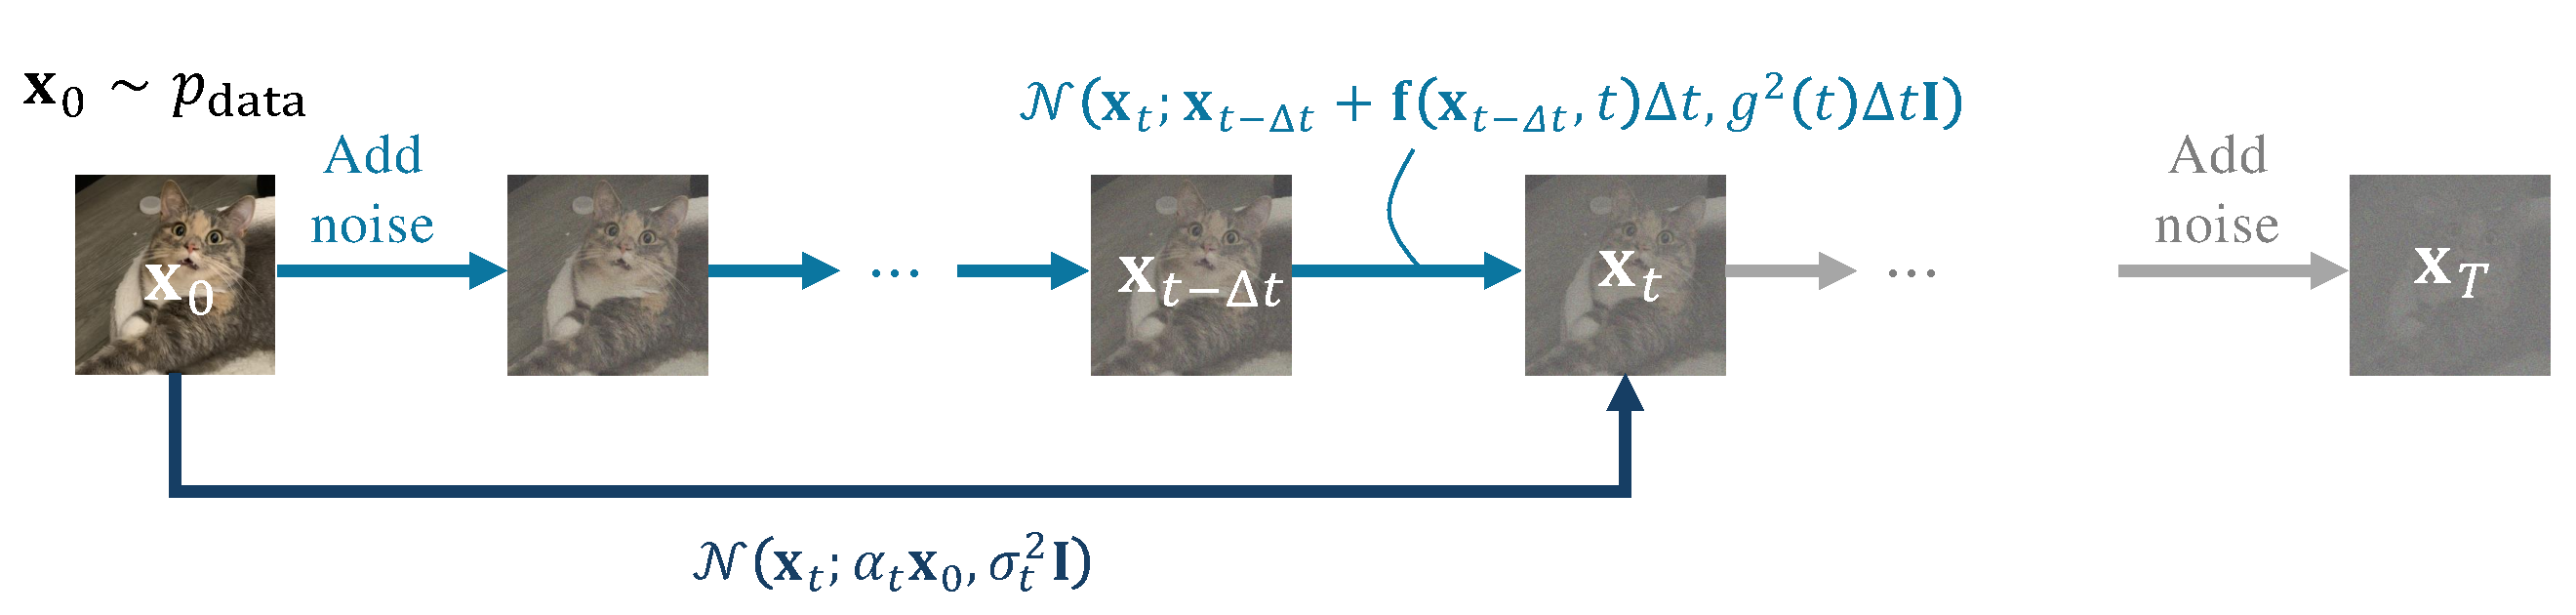
\includegraphics[width=\linewidth]{Images/PartB/vdm-sde.pdf}
    \caption{\textbfs{引理~\ref{forward-sde} 的示意图。}通过连续时间 SDE（$\Delta t\to 0$）的增量噪声注入与 \Cref{eq:forward_kernel} 的直接扰动在数学上等价。 \figcredit{由作者绘制。}}
    \label{fig:vdm-sde}
\end{figure}
\subsection{一般的仿射前向过程 $p_t(\rvx_t |\rvx_0)$}
我们先定义一个一般的前向扰动核：
\begin{equation}\label{eq:forward_kernel}
p_t(\rvx_t| \rvx_0) := \mathcal{N}\big(\rvx_t; \alpha_t \rvx_0, \sigma_t^2 \mathbf{I}\big),
\end{equation}
其中 $\rvx_0 \sim p_{\mathrm{data}}$，$\alpha_t$、$\sigma_t$ 是 $t \in [0,T]$ 的非负标量函数，满足：
\begin{enumerate}
    \item[(i)] 对所有 $t \in (0,1]$，$\alpha_t > 0$ 且 $\sigma_t > 0$（允许 $\sigma_0 = 0$），且
    \item[(ii)] 通常 $\alpha_0 = 1$ 且 $\sigma_0 = 0$。
\end{enumerate}
也就是说，$\rvx_t \sim p_t(\rvx_t | \rvx_0)$ 可以采样为
\begin{equation*}
\rvx_t = \alpha_t \rvx_0 + \sigma_t \bm{\epsilon}, 
\qquad \bm{\epsilon} \sim \mathcal{N}(\mathbf{0}, \mathbf{I}).
\end{equation*}

这一框架涵盖了若干著名的实例，包括 VE（例如 NCSN）、VP（例如 DDPM）以及流匹配（FM）前向核~\citep{lipman2022flow, liu2022rectified}，后者在 $\rvx_0$ 和 $\bm{\epsilon}$ 之间做线性插值（见后文 \Cref{sec:flow-matching-framework}）。
\begin{itemize}
\item \textbfs{VE（NCSN）核：}$\alpha_t \equiv 1$，$\sigma_T \gg 1$；
\item \textbfs{VP（DDPM）核：}$\alpha_t := \sqrt{1 - \sigma_t^2}$，使得 $\alpha_t^2 + \sigma_t^2 = 1$；
\item \textbfs{FM 核：}$\alpha_t = 1 - t$，$\sigma_t = t$。
\end{itemize}

\subsection{与 Score SDE 的联系}
对 Score SDE 而言，以线性形式指定 $ p_t(\rvx_t|\rvx_0) $ 自然地诱导出一个具有仿射系数的 SDE，这提供了比从漂移项和扩散项出发、为各矩求解 ODE（见 \Cref{subsec:scoresde-perturbation-kernel}）更直观的替代方案。

给定 \Cref{eq:forward_kernel} 中的前向扰动核，相应的前向 SDE 取如 \Cref{eq:forward-linear-sde} 的关于 $\rvx$ 线性的形式：
\begin{align*}
    \diff \rvx(t) = \underbrace{f(t)\rvx(t)}_{\rvf(\rvx(t), t)} \diff t + g(t) \diff\rvw(t),
\end{align*}
其中 $ f, g\colon [0,T] \rightarrow \mathbb{R} $ 是时间的实值函数。
系数 $ f(t) $ 和 $ g(t) $ 可以用 $ \alpha_t $ 和 $ \sigma_t $ 解析地表达，如下面的引理所总结。

\lemp{前向扰动核 $\Leftrightarrow$ 线性 SDE}{forward-sde}{ 对 $t\in(0,T]$ 定义 $\lambda_t:=\log\tfrac{\alpha_t}{\sigma_t}$。
给定前向扰动核
\[
\rvx_t=\alpha_t \rvx_0+\sigma_t \beps,\qquad \beps\sim\mathcal N(\mathbf 0,\rmI),
\]
线性 SDE
\[
\diff \rvx(t)=f(t) \rvx(t) \diff t+g(t) \diff\rvw(t),
\]
其系数为
\begin{align}\label{eq:kernel-sde-equiv}
\begin{aligned}
f(t)&=\frac{\diff}{\diff t}\log \alpha_t,\\
g^2(t)&=\frac{\diff \sigma_t^2}{\diff t}-2\frac{\diff}{\diff t}\log\alpha_t \sigma_t^2
       = -2\sigma_t^2 \frac{\diff}{\diff t}\lambda_t,
\end{aligned}
\end{align}
对所有 $t\in(0,T]$ 具有条件转移 $p_t(\rvx_t|\rvx_0)=\mathcal N \big(\rvx_t;\alpha_t\rvx_0,\sigma_t^2\rmI\big)$。
反之，若一个线性 SDE 的条件转移为 $\mathcal N(\rvx_t;\alpha_t\rvx_0,\sigma_t^2\rmI)$，使得对所有 $t\in(0,T]$ 都有 $\alpha_t>0$ 且 $\sigma_t>0$，则其系数对 $t\in(0,T]$ 满足 \Cref{eq:kernel-sde-equiv}。
}{由 \Cref{subsec:scoresde-perturbation-kernel}，证明就是将均值与协方差 ODE $\rvm'(t) = f(t)\rvm(t)$、$\rmP'(t) = 2f(t) \rmP(t) + g^2(t) \rmI$ 与
$\rvm(t)=\alpha_t\rvx_0$ 和 $\rmP(t)=\sigma_t^2\rmI$（在 $(0,T]$ 上）相匹配。}


\rmkb{要在终止时刻精确匹配一个高斯先验，过程必须完全遗忘 $\rvx_0$ 并达到目标方差；这要求 $\alpha_T=0$ 且 $\sigma_T^2$ 等于先验方差。

在 SDE 表述中，有
\[
\alpha_t=\exp \Big(\int_0^t f(u)\diff  u\Big).
\]
因此，在有限 $T$ 处强制 $\alpha_T=0$ 会迫使
\[
\int_0^T f(u)\diff u=-\infty,
\]
意味着漂移项必须随 $t\rightarrow T$ 无限快地收缩。
同时，扩散必须发散以维持所规定的方差，这反映在
\[
g^2(t)=\sigma_t^{2 \prime}-2\frac{\alpha_t'}{\alpha_t} \sigma_t^2  \rightarrow  \infty
\quad\text{as } t\rightarrow T.
\]

如果 $f$ 和 $g$ 在 $[0,T]$ 上保持有界，则必然有 $\alpha_T>0$ 且仍残留对 $\rvx_0$ 的依赖。此时，高斯先验只能渐近地达到：要么在 $t\to T$ 的极限下（但不能精确达到），要么在适当的时间重参数化后于 $T\to\infty$ 的无穷区间上精确达到。
}


由上述引理，通过具有系数 $f(t)$ 和 $g(t)$ 的线性 SDE 指定增量噪声注入，在数学上等价于以参数 $\alpha_t$ 和 $\sigma_t$ 定义扰动核。在扩散模型文献中，这两种视角可互换使用。因此，我们得出结论：
\msg{观察}{}{
定义 $p_t(\rvx_t | \rvx_0)$ 等价于指定线性 SDE 的系数 $f(t)$ 和 $g(t)$。
}


\subsection{与基于变分的扩散模型的联系}\label{subsec:connection-vdm}
我们重新审视 DDPM 中一个通过贝叶斯法则推导的核心恒等式：
\begin{align}\label{eq:ddpm-reverse-condition-kernel}
    p(\rvx_{t-\Delta t}|\rvx_t, \rvx) = p(\rvx_t|\rvx_{t-\Delta t}) \cdot \frac{p_{t-\Delta t}(\rvx_{t-\Delta t}|\rvx)}{p_t(\rvx_t|\rvx)},
\end{align}
对任意 $\rvx$（通常 $\rvx\sim p_{\mathrm{data}}$）。这一反向条件 $ p(\rvx_{t-\Delta t} | \rvx_t, \rvx) $ 是建模的核心，使得易于处理的训练目标与高效采样成为可能。

虽然 DDPM 通常先定义增量核 $p(\rvx_t|\rvx_{t-\Delta t})$，但累积转移 $p_t(\rvx_t|\rvx_0)$ 往往提供更具可解释性、更实用的表述，尤其对于先验和损失设计而言。

\paragraph{推导转移核。}
我们现在将其推广到连续时间设定。设 $0 \leq t < s \leq T$ 为两个（连续）时间点。给定扰动核 $p_t(\rvx_t|\rvx_0)$，我们可以通过应用 \Cref{eq:ddpm-reverse-condition-kernel}\footnote{这一恒等式自然地推广到连续时间，只需把 $s$ 视为一个一般的较早时刻。}，以前向核 $p(\rvx_s|\rvx_t)$ 为中间量，对任意 $\rvx$ 计算反向条件 $p(\rvx_t|\rvx_s, \rvx)$。下面的引理总结了这一推导，它推广了引理~\ref{ddpm-reverse-kernel}，且不假设 $\alpha_t^2 + \sigma_t^2 = 1$。

\lemp{反向条件转移核}{reverse-kernel}{
设 $0 \leq t < s \leq T$。反向\emph{条件}转移核为：
\begin{equation*}
    p(\rvx_t|\rvx_s, \rvx) = \mathcal{N}\left(\rvx_t; \bm{\mu}(\rvx_s, \rvx; s, t), \sigma^2(s, t) \bfI\right),
\end{equation*}
其中
\begin{align}\label{eq:p_backward_mean_var}
\begin{aligned}
    \bm{\mu}(\rvx_s, \rvx; s, t) := \frac{\alpha_{s|t} \sigma_t^2}{\sigma_s^2} \rvx_s + \frac{\alpha_t \sigma^2_{s|t}}{\sigma_s^2} \rvx, \quad
    \sigma^2(s, t) := \sigma^2_{s|t} \frac{\sigma_t^2}{\sigma_s^2}.
\end{aligned}
\end{align}
这里，$\alpha_{s|t}$ 和 $\sigma_{s|t}$ 定义为：
\begin{equation*}
    \alpha_{s|t} := \frac{\alpha_s}{\alpha_t}, \qquad \sigma^2_{s|t} := \sigma_s^2 - \alpha_{s|t}^2 \sigma_t^2.
\end{equation*}
}{
我们首先计算前向转移核：
\begin{equation}\label{eq:zt_given_zs}
    p(\rvx_s|\rvx_t) = \mathcal{N}\left(\rvx_s; \alpha_{s|t} \rvx_t, \sigma^2_{s|t} \bfI\right).
\end{equation}
反向核随后由贝叶斯法则给出，由于所有涉及的分布都是高斯，结果可直接计算得到。更多细节见 \citep{kingma2021variational} 的附录 A。
}


尽管 $p(\rvx_{t + \Delta t}|\rvx_t)$ 与 $p_t(\rvx_t|\rvx_0)$ 在理论上是等价的，但 $p_t(\rvx_t|\rvx_0)$ 往往扮演更核心的角色。\Cref{eq:zt_given_zs} 中的逐步转移主要用于得到闭式的反向核。因此，近期的工作~\citep{kingma2021variational} 倾向于直接指定 $p_t(\rvx_t|\rvx_0)$，以获得清晰性与可解释性。



\paragraph{反向过程建模、训练与采样。}
\Cref{eq:ddpm-elbo} 中的训练目标（ELBO）以及 \Cref{sec:ddpm} 中引入的建模框架在我们推广的设定下仍然适用。为清楚起见，遵循~\citet{kingma2021variational}，我们采用 $\rvx$-预测的表述，记为 $\rvx_{\bm{\phi}}(\rvx_s, s)$。然而，等价的 $\beps$-预测视角（以 $\bm{\epsilon}_{\bm{\phi}}(\rvx_s, s)$ 表示）同样有效，因为存在如下关系（如 \Cref{eq:ddpm-clean-noise}）
\[
\rvx_s = \alpha_s \rvx_{\bm{\phi}}(\rvx_s, s) + \sigma_s \bm{\epsilon}_{\bm{\phi}}(\rvx_s, s),\quad \text{for any given } \rvx_s \sim q_s.
\]

\subparagraph{建模与扩散损失 $\mathcal{L}_{\text{diffusion}}$。}
与 DDPM 类似，\Cref{eq:p_backward_mean_var} 中的条件分布 $p(\rvx_t|\rvx_s, \rvx)$ 启发我们将干净信号 $\rvx$ 替换为一个可学习的预测器 $\rvx_{\bm{\phi}}(\rvx_s, s)$，得到如下参数化的反向模型：
\begin{align}\label{eq:general-ddpm-sampling}
    p_{\bm{\phi}}(\rvx_t | \rvx_s) := \mathcal{N}\left(\rvx_t; \bm{\mu}_{\bm{\phi}}(\rvx_s, s, t), \sigma^2(s,t) \mathbf{I}\right),
\end{align}
其均值参数化为：
\[
    \bm{\mu}_{\bm{\phi}}(\rvx_s, s, t) = \frac{\alpha_{s|t} \sigma_t^2}{\sigma_s^2} \rvx_s + \frac{\alpha_t \sigma_{s|t}^2}{\sigma_s^2} \rvx_{\bm{\phi}}(\rvx_s, s).
\]
给定 \Cref{eq:forward_kernel} 中的前向核，$\mathcal{L}_{\text{diffusion}}(\rvx; \bm{\phi})$ 中的 KL 散度退化为一个加权回归损失：
\begin{align}
\begin{aligned}
    \label{eq:snr-kl}
    \mathcal{D}_{\text{KL}}\big(p(\rvx_t|\rvx_s, \rvx_0)  \| p_{\bm{\phi}}(\rvx_t|\rvx_s)\big)  
    &= \frac{1}{2\sigma^2(s,t)} \left\| \bm{\mu}(\rvx_s, \rvx_0; s,t) - \bm{\mu}_{\bm{\phi}}(\rvx_s, s, t) \right\|_2^2 \\
    &= \frac{1}{2} \big(\text{SNR}(t) - \text{SNR}(s)\big) \left\| \rvx_0 - \rvx_{\bm{\phi}}(\rvx_s, s) \right\|_2^2,
\end{aligned}
\end{align}
其中 $\rvx_s = \alpha_s\rvx_0 + \sigma_s\bm{\epsilon}$，$\rvx_0 \sim p_{\mathrm{data}}$，$\bm{\epsilon} \sim \mathcal{N}(\bm{0}, \rmI)$，$\text{SNR}(s) := \alpha_s^2 / \sigma_s^2$ 表示时刻 $s$ 的信噪比。


\rmkb{
在 \citep{kingma2021variational} 中，作者研究 \Cref{eq:snr-kl} 当 $t \to s$ 时的连续时间极限，得到：
\begin{align*}
\mathcal{L}_{\text{VDM}}^\infty(\rvx_0) 
= -\frac{1}{2}  \mathbb{E}_{s, \bm{\epsilon} \sim \mathcal{N}(\bm{0}, \bfI)}  \text{SNR}'(s)  \big\| \rvx_0 - \rvx_{\bm{\phi}}(\rvx_s, s) \big\|_2^2.
\end{align*}
这一设定还引入了一个可学习的噪声调度，虽然它可推广到连续型数据之外，但这种扩展超出了我们当前讨论的范围。
}

\subparagraph{采样。}
采样过程与 DDPM 类似，使用 \Cref{eq:general-ddpm-sampling} 中的参数化核：
\begin{align}\label{eq:general-ddpm-sampling-discrete}
    \rvx_t = \underbrace{\frac{\alpha_{s|t} \sigma_t^2}{\sigma_s^2} \rvx_s + \frac{\alpha_t \sigma_{s|t}^2}{\sigma_s^2} \rvx_{\bm{\phi}^\times}(\rvx_s, s)}_{\bm{\mu}_{\bm{\phi}^\times}(\rvx_s, t, s)} + \sigma_{s|t} \frac{\sigma_t}{\sigma_s} \bm{\epsilon}_s,\quad  \bm{\epsilon}_s \sim \mathcal{N}(\bm{0}, \rmI).
\end{align}



\clearpage
\newpage

\section{（选读）Fokker–Planck 方程与反向时间 SDE \\——通过边缘化与贝叶斯法则}\label{eq:heuristic-fpe-sde}
本节中，我们提供关于 Fokker–Planck 方程与反向时间 SDE 结构的概率视角。通过借助边缘化技巧与贝叶斯法则等基本工具，我们阐明随机过程的统计表述与其相应微分方程之间的联系。

我们强调，此处给出的``推导''并非数学上严格的证明，而只是旨在传达底层联系的启发性论证。


\subsection{由转移核边缘化得到的 Fokker-Planck 方程}\label{subsec:fpe-reason}
给定如 \Cref{eq:transition-forward-f-g} 的前向转移概率
\begin{align*}
    p(\mathbf{x}_{t+\Delta t} | \mathbf{x}_t) = \mathcal{N}\left(\mathbf{x}_{t+\Delta t}; \mathbf{x}_t + \mathbf{f}(\mathbf{x}_t, t)\Delta t, g^2(t)\Delta t \mathbf{I}\right),
\end{align*}
以及边缘分布
\begin{align*}
    p_t(\mathbf{x}_t), \quad p_{t+\Delta t}(\mathbf{x}_{t+\Delta t}),
\end{align*}
我们的目标是推导支配边缘分布 $p_t$ 时间演化的 Fokker-Planck 方程。


\paragraph{变量替换。}
由马尔可夫性，时刻 $t + \Delta t$ 的边缘分布可以表示为对前一状态 $\mathbf{x}_t$ 的积分（即 Chapman-Kolmogorov 方程）：
\begin{align*}
p_{t+\Delta t}(\rvx)
= \int \mathcal N \big(\rvx; \rvy+\rvf(\rvy,t)\Delta t, g^2(t)\Delta t \rmI\big) p_t(\rvy) \diff\rvy.
\end{align*}
 我们引入一个新变量
\[
\rvu  :=  \rvy+\rvf(\rvy,t)\Delta t,
\]
于是该高斯以 $\rvu$ 为中心。对于小的 $\Delta t$，这个映射可逆，且
\[
\rvy  =  \rvu-\rvf(\rvu,t)\Delta t+\mathcal O(\Delta t^2),
\quad
\Bigg|\det\frac{\partial \rvy}{\partial \rvu}\Bigg|
 = 1-(\nabla_\rvu \cdot\rvf)(\rvu,t) \Delta t+\mathcal O(\Delta t^2).
\]
因此，变量替换公式给出：
\begin{align*}
    p_{t+\Delta t}(\rvx)
&= \int \mathcal N\left(\rvx;\rvu,g^2(t)\Delta t\rmI\right) \cdot
\\\quad\Big[p_t(\rvu)&-\Delta t \rvf(\rvu,t) \cdot \nabla_\rvu p_t(\rvu)
-\Delta t (\nabla_\rvu \cdot\rvf)(\rvu,t) p_t(\rvu)\Big] \diff\rvu
+\mathcal O(\Delta t^2),
\end{align*}

\paragraph{泰勒展开。}
对任意光滑函数 $\phi:\R^D\to\R$ 和尺度 $\sigma>0$，
若 $\rvz\sim\mathcal N(\bm{0},\rmI)$，如下近似成立
（即 \emph{Taylor–高斯光滑公式}）：

\[
\int \mathcal N(\rvx;\rvu,\sigma^2\rmI) \phi(\rvu) \diff\rvu
=\E \left[\phi(\rvx+\sigma\rvz)\right]
=\phi(\rvx)+\frac{\sigma^2}{2} \Delta_\rvx\phi(\rvx)+\mathcal O(\sigma^4).
\]
这是因为对如下的泰勒展开：
\[
\phi(\rvx+\sigma\rvz)=\phi(\rvx)+\sigma\nabla_\rvx\phi(\rvx) \cdot \rvz+\frac{\sigma^2}{2}\rvz^\top\nabla_\rvx^2\phi(\rvx)\rvz+\mathcal O(\sigma^3)
\]
以及 $\E[\rvz]=\bm{0}$，$\E[\rvz\rvz^\top]=\rmI$。

以 $\phi=p_t$、$\phi=\rvf \cdot \nabla_\rvu p_t$ 和 $\phi=(\nabla_\rvu \cdot\rvf) p_t$ 应用此公式，并取 $\sigma^2=g^2(t)\Delta t$，可得
\[
\begin{aligned}
&p_{t+\Delta t}(\rvx) - p_t(\rvx)
\\=& -\Delta t \rvf(\rvx,t) \cdot \nabla_\rvx p_t(\rvx)
-\Delta t (\nabla_\rvx \cdot\rvf)(\rvx,t) p_t(\rvx)
+\frac{g^2(t)}{2}\Delta t \Delta_\rvx p_t(\rvx)
+\mathcal O(\Delta t^2) 
\\=&  - \Delta t \nabla_\rvx \cdot \big(\rvf(\rvx,t) p_t(\rvx)\big)
 + \frac{g^2(t)}{2} \Delta t \Delta_\rvx p_t(\rvx)
 + \mathcal O(\Delta t^2).
\end{aligned}
\]
除以 $\Delta t$ 并令 $\Delta t\to0$，即得 Fokker–Planck 方程。

在 \Cref{subsec:rigorous-proof-fpe} 中，我们给出基于 It\^o 的推导，以补充上述离散时间视角。




\subsection{反向时间 SDE 为何取这种形式？}\label{subsec:reverse-sde-reason}

反向时间 SDE 的严格推导是技术性的，需要深入 Fokker-Planck 方程的性质。然而，反向时间 SDE 的形式可以通过贝叶斯定理直观地理解。这里，我们给出一个启发性推导，以提供 \Cref{eq:sde_backward} 为何取其形式、且分数函数为何出现的洞察\footnote{这一推导受到 \href{https://alexxthiery.github.io/notes/reverse_and_tweedie/reverse_and_tweedie.html}{此帖} 中方法的启发。}。


\paragraph{利用贝叶斯法则进行反演。}
我们的目标是通过先考虑离散时间情形来确定反向时间转移核：
\[
p(\rvx_t | \rvx_{t+\Delta t}),
\]
然后取 $\Delta t \rightarrow 0$ 以得到连续时间的表述。
由贝叶斯定理，我们表达：
\begin{align}\label{eq:reverse-sde-bayes-discrete}
    p(\rvx_t | \rvx_{t+\Delta t}) 
    &= p(\rvx_{t+\Delta t} | \rvx_t) \frac{p_t(\rvx_t)}{p_{t+\Delta t}(\rvx_{t+\Delta t})} \nonumber \\
    &= p(\rvx_{t+\Delta t} | \rvx_t) \exp\left(\log p_t(\rvx_t) - \log p_{t+\Delta t}(\rvx_{t+\Delta t})\right).
\end{align}

前向转移核假设如 \Cref{eq:transition-forward-f-g}：
\begin{equation*}
p(\rvx_{t+\Delta t} | \rvx_t) = \mathcal{N}\left(\rvx_{t+\Delta t}; \rvx_t + \rvf(\rvx_t, t)\Delta t, g^2(t)\Delta t \mathbf{I}\right)
\end{equation*}

\paragraph{泰勒展开。}
为处理指数项，我们应用一阶泰勒展开。关键的洞察是在空间和时间两个维度上围绕点 $(\rvx_t, t)$ 展开：
\begin{align*}
    \log p_{t+\Delta t}(\rvx_{t+\Delta t}) &= \log p_t(\rvx_t) + \nabla_{\rvx} \log p_t(\rvx_t) \cdot (\rvx_{t+\Delta t} - \rvx_t) \nonumber \\
    &\quad + \frac{\partial \log p_t(\rvx_t)}{\partial t} \Delta t + \mathcal{O}(\|\rvh\|_2^2) 
\end{align*}
其中 $\rvh := (\rvx_{t+\Delta t} - \rvx_t, \Delta t)$。因此：
\begin{align}
    \log p_t(\rvx_t) - \log p_{t+\Delta t}(\rvx_{t+\Delta t}) &= -\nabla_{\rvx} \log p_t(\rvx_t) \cdot (\rvx_{t+\Delta t} - \rvx_t) \nonumber \\
    &\quad - \frac{\partial \log p_t(\rvx_t)}{\partial t} \Delta t + \mathcal{O}(\|\rvh\|_2^2) \label{eq:log-difference}
\end{align}

对于具有有限漂移和扩散的前向过程，有 $\mathbb{E}[\|\rvx_{t+\Delta t} - \rvx_t\|_2^2] = \mathcal{O}(\Delta t)$，这确保余项在期望意义下为 $\mathcal{O}((\Delta t)^2)$。

\paragraph{代入反向转移。}
将方程 \Cref{eq:transition-forward-f-g} 和 \Cref{eq:log-difference} 代入 \Cref{eq:reverse-sde-bayes-discrete}：
\begin{align*}
    &p(\rvx_t | \rvx_{t+\Delta t}) \nonumber \\
    = &\frac{1}{(2\pi g^2(t) \Delta t)^{D/2}} \exp\left(-\frac{\|\rvx_{t+\Delta t} - \rvx_t - \rvf(\rvx_t, t) \Delta t\|_2^2}{2 g^2(t) \Delta t}\right) \nonumber \\
    &\qquad \cdot \exp\left(-\nabla_{\rvx} \log p_t(\rvx_t) \cdot (\rvx_{t+\Delta t} - \rvx_t) - \frac{\partial \log p_t(\rvx_t)}{\partial t} \Delta t + \mathcal{O}((\Delta t)^2)\right). 
\end{align*}
\paragraph{代数操作。}
关键的一步是在指数中配方。我们有：
\begin{align*}
    &-\frac{\|\rvx_{t+\Delta t} - \rvx_t - \rvf(\rvx_t, t) \Delta t\|_2^2}{2 g^2(t) \Delta t} - \nabla_{\rvx} \log p_t(\rvx_t) \cdot (\rvx_{t+\Delta t} - \rvx_t) \nonumber \\
    = &-\frac{\left[\|\rvx_{t+\Delta t} - \rvx_t - \rvf(\rvx_t, t) \Delta t\|_2^2 + 2 g^2(t) \Delta t \nabla_{\rvx} \log p_t(\rvx_t) \cdot (\rvx_{t+\Delta t} - \rvx_t)\right]}{2 g^2(t) \Delta t} 
\end{align*}
令 $\boldsymbol{\delta} := \rvx_{t+\Delta t} - \rvx_t$ 和 $\boldsymbol{\mu} := \rvf(\rvx_t, t) \Delta t$。则：
\begin{align*}
    &\|\boldsymbol{\delta} - \boldsymbol{\mu}\|_2^2 + 2 g^2(t) \Delta t \nabla_{\rvx} \log p_t(\rvx_t) \cdot \boldsymbol{\delta} \nonumber \\
    = &\|\boldsymbol{\delta}\|_2^2 - 2\boldsymbol{\delta} \cdot \boldsymbol{\mu} + \|\boldsymbol{\mu}\|_2^2 + 2 g^2(t) \Delta t \nabla_{\rvx} \log p_t(\rvx_t) \cdot \boldsymbol{\delta} \nonumber \\
    = &\|\boldsymbol{\delta}\|_2^2 - 2\boldsymbol{\delta} \cdot [\boldsymbol{\mu} - g^2(t) \Delta t \nabla_{\rvx} \log p_t(\rvx_t)] + \|\boldsymbol{\mu}\|_2^2 \nonumber \\
    = &\|\boldsymbol{\delta} - [\boldsymbol{\mu} - g^2(t) \Delta t \nabla_{\rvx} \log p_t(\rvx_t)]\|_2^2 - \|g^2(t) \Delta t \nabla_{\rvx} \log p_t(\rvx_t)\|_2^2 
\end{align*}
代回：
\begin{align*}
    &\|\boldsymbol{\delta} - [\rvf(\rvx_t, t) \Delta t - g^2(t) \Delta t \nabla_{\rvx} \log p_t(\rvx_t)]\|_2^2 \nonumber \\
    = &\|\rvx_{t+\Delta t} - \rvx_t - [\rvf(\rvx_t, t) - g^2(t) \nabla_{\rvx} \log p_t(\rvx_t)] \Delta t\|_2^2. 
\end{align*}
因此，
\begin{align*}
    p(\rvx_t | \rvx_{t+\Delta t}) 
    =~&\frac{1}{(2\pi g^2(t) \Delta t)^{D/2}} \nonumber \\
    \quad &\cdot \exp\left(-\frac{\|\rvx_{t+\Delta t} - \rvx_t - [\rvf(\rvx_t, t) - g^2(t) \nabla_{\rvx} \log p_t(\rvx_t)] \Delta t\|_2^2}{2 g^2(t) \Delta t}\right) \nonumber \\
    \quad &\cdot \exp(\mathcal{O}(\Delta t)) \nonumber \\
    =~&\mathcal{N}\left(\rvx_t; \rvx_{t+\Delta t} - [\rvf(\rvx_t, t) - g^2(t) \nabla_{\rvx} \log p_t(\rvx_t)] \Delta t, g^2(t) \Delta t \mathbf{I}\right) \nonumber \\
    \quad &\cdot (1 + \mathcal{O}(\Delta t)).
\end{align*}
配方所产生的附加项 $\|g^2(t) \Delta t \nabla_{\rvx} \log p_t(\rvx_t)\|_2^2$ 为 $\mathcal{O}((\Delta t)^2)$，可吸收进误差项。类似地，时间导数项 $\frac{\partial \log p_t(\rvx_t)}{\partial t} \Delta t$ 为 $\mathcal{O}(\Delta t)$，在连续极限下会消失。

\paragraph{取 $\Delta t \rightarrow 0$ 的极限。}
当 $\Delta t \approx 0$ 时，在光滑性假设下，如下近似成立：
\begin{align*}
    \rvf(\rvx_t, t) &\approx \rvf(\rvx_{t+\Delta t}, t+\Delta t), \\
    g(t) &\approx g(t+\Delta t), \\
    \nabla_{\rvx} \log p_t(\rvx_t) &\approx \nabla_{\rvx} \log p_{t+\Delta t}(\rvx_{t+\Delta t})  = \rvs(\rvx_{t+\Delta t}, t+\Delta t).
\end{align*}
利用这些近似以及一些重排，我们得到：
\begin{align*}
    &p(\rvx_t | \rvx_{t+\Delta t}) \\ \approx &\frac{1}{(2\pi g^2(t) \Delta t)^{D/2}}  \exp \Bigg(
            \\ &-\frac{\Big\|\rvx_{t} - \Big(\rvx_{t+\Delta t} - \big[\rvf(\rvx_{t+\Delta t}, t+\Delta t) - g^2({t+\Delta t}) \rvs(\rvx_{t+\Delta t}, t+\Delta t)\big] \Delta t\Big) \Big\|_2^2 }{2 g^2(t+\Delta t) \Delta t} \\
            &\Bigg).
\end{align*}
这意味着 $p(\rvx_t | \rvx_{t+\Delta t})$ 近似为一个正态分布，其：
\begin{align*}
    \text{\textbfs{均值：}} &  \quad\rvx_{t+\Delta t} - \big[\rvf(\rvx_{t+\Delta t}, t+\Delta t) - g^2(t+\Delta t) \rvs (\rvx_{t+\Delta t}, t+\Delta t)\big] \Delta t, \\
    \text{\textbfs{协方差：}} & \quad g^2(t+\Delta t) \Delta t \mathbf{I}.
\end{align*}
取 $\Delta t \rightarrow 0$ 的极限，我们``推导''出 \Cref{eq:sde_backward} 中给出的反向时间连续 SDE。








\clearpage
\newpage

\section{结束语}


本章标志着我们旅程中的一个关键时刻，将来自变分视角与分数基视角的离散时间扩散过程统一为一个优雅的连续时间框架。我们证明了 DDPM 与 NCSN 都可以理解为具有不同漂移/波动率系数的随机微分方程（SDE）的离散化。

这一框架的基石是存在一个相应的反向时间 SDE，它形式化地定义了一个逆转噪声破坏的生成过程。关键的是，这一反向过程的漂移项仅依赖于一个未知量：在每个时刻的边缘数据分布的分数函数 $\nabla_{\mathbf{x}}\log{p_{t}(\mathbf{x})}$。这一洞见巩固了分数函数在生成式建模中的核心地位。

此外，我们引入了一个纯确定性的对应物——概率流常微分方程（PF-ODE），其解轨迹沿与 SDE 相同的边缘密度 $\{p_{t}\}$ 演化。这种显著的一致性由底层的 Fokker-Planck 方程保证。其深远的含义是：生成这一复杂任务在根本上等价于求解一个微分方程。训练归结为学习定义该方程向量场的分数函数，而采样则成为数值积分的问题。

PF-ODE 这一纯确定性流的引入，为扩散模型的第三个、也是最后一个视角搭建了一座有力的桥梁。学习一个由速度场支配的确定性变换这一概念，是近期一大类重要生成模型的核心原理。在下一章中，我们将：
\begin{enumerate}
    \item 探索这种基于流的视角，从其在归一化流与神经 ODE 中的起源开始。
    \item 展示这一观点如何引出现代的流匹配框架，该框架直接学习一个速度场以在分布之间传输样本。
\end{enumerate}

最终，我们将看到，从随机原理推导出的确定性 PF-ODE，如何能够从这种完全不同的、基于流的起源出发被构造与推广，从而完成我们对扩散建模的统一图景。



% \msg{}{From the derivation, we can conceptually understand that Bayes' rule in \Cref{eq:reverse-sde-bayes-discrete},
% \begin{align*}
%     p(\rvx_t |\rvx_{t+\Delta t})  
%     = p(\rvx_{t+\Delta t} |\rvx_t) \cdot \frac{p_t(\rvx_t)}{p_{t+\Delta t}(\rvx_{t+\Delta t})},
% \end{align*}
% serves as a discrete-time approximation of the reverse-time SDE, with an approximation error of order $ \abs{\Delta t} $.
% }



% \newpage

% \subsection{A Conceptual Variational Derivation of the Shared Fokker–Planck Equation for Forward and Reverse Processes}\label{subsec:conceptual-same-fokker-planck}

% In \Cref{subsec:fpe-sde-ode}, we observed that the reverse-time SDE is constructed to match the marginal distributions of the forward SDE, thereby mapping the noise distribution back to the data distribution. In this section, we develop an intuitive understanding of why the reverse-time dynamics—at the level of transition probabilities—should mirror those of the forward process, viewed from a variational perspective in discrete time.



% We begin by defining the forward transition kernel as follows:
% \begin{align*}
%     p(\rvx_{t+\Delta t} | \rvx_t) = \mathcal{N}\left(\rvx_{t+\Delta t}; \rvx_t + \rvf(\rvx_t, t)\Delta t, g^2(t)\Delta t \mathbf{I}\right),
% \end{align*}
% where the initial distribution is given by $p_0 = p_{\mathrm{data}}$.

% \paragraph{Forward Process.}
% We revisit the formulation in \Cref{subsec:fpe-reason}, introducing slightly revised notations for consistency with the reverse process discussed later. Given the specified forward transition kernel, we can compute the conditional distribution $p_t(\rvx_t|\rvx_0)$, which in turn induces the marginal distribution at time $t$:
% \begin{align*}
% p_{t}^{\text{fwd}}(\rvx_t) := \int p_t(\rvx_t|\rvx_0)  p_{\mathrm{data}}(\rvx_0)  \diff\rvx_0.
% \end{align*}

% From the Chapman-Kolmogorov equation, the forward evolution satisfies
% \begin{align*}
% p_{t+\Delta t}^{\text{fwd}}(\rvx_{t+\Delta t}) = \int p(\rvx_{t+\Delta t}|\rvx_t) p_{t}^{\text{fwd}}(\rvx_t) \diff\rvx_t.
% \end{align*}
% Therefore, we can obtain the 
% \begin{align*}
% p_{t+\Delta t}^{\text{fwd}}(\rvx) - p_{t}^{\text{fwd}}(\rvx) = \left[-\nabla \cdot [\rvf(\rvx, t) p_t^{\text{fwd}}(\rvx)] + \frac{g^2(t)}{2} \nabla^2 p_t^{\text{fwd}}(\rvx)\right] \Delta t + \mathcal O(\Delta t^2).
% \end{align*}

% \paragraph{Reverse Process.}

% The reverse process evolves backward in time from the terminal distribution. Starting with $p_{0}^{\text{rev}} := p_{T}^{\text{fwd}}$, by Bayes' rule, we have when $\Delta t \approx 0$
% \begin{align*}
%     &p(\rvx_{t-\Delta t}|\rvx_t) \\
%     =~&p(\rvx_{t}|\rvx_{t-\Delta t}) \frac{p_{t-\Delta t}^{\text{fwd}}(\rvx_{t-\Delta t})}{p_t^{\text{fwd}}(\rvx_t)} \\
%     =~&p(\rvx_{t}|\rvx_{t-\Delta t}) \exp\left(\log p_{t-\Delta t}^{\text{fwd}}(\rvx_{t-\Delta t}) - \log p_{t}^{\text{fwd}}(\rvx_{t})\right) \\
%     =~&\mathcal{N}\left(\rvx_{t-\Delta t}; \rvx_{t} - \big[\rvf(\rvx_{t}, t) - g^2(t) \rvs (\rvx_{t}, t)\big] \Delta t, g^2(t) \Delta t \mathbf{I}\right) \nonumber   \cdot (1 + \mathcal{O}(\Delta t)),
% \end{align*}
% where $\rvs(\rvx_t, t) = \nabla \log p_t^{\text{fwd}}(\rvx_t)$ is the score function.
% With this, it induces the reverse perturbation kernel $p^{\text{rev}}(\rvx_t|\rvx_0)$ and the reverse marginal distribution: 
% \begin{align*}
% p_{t}^{\text{rev}}(\rvx_t) &:= \int p^{\text{rev}}(\rvx_t|\rvx_0) p_{0}^{\text{rev}}(\rvx_0)\diff\rvx_0.
% \end{align*}

% By the Markov property and the marginal consistency condition (as formalized by the Chapman–Kolmogorov equation), the reverse-time marginal satisfies
% \begin{align*}
% p_{t-\Delta t}^{\text{rev}}(\rvx_{t-\Delta t}) = \int p(\rvx_{t-\Delta t}|\rvx_t)  p_{t}^{\text{rev}}(\rvx_t)  \diff\rvx_t.
% \end{align*}
% Following analogous steps to the forward case, we substitute the reverse transition kernel and write $\rvx= \rvx_{t-\Delta t}$ and $\rvy = \rvx_t$:
% \begin{align*}
% p_{t-\Delta t}^{\text{rev}}(\rvx) \approx \int \mathcal{N}(\rvx; \mathbf{y} - [\rvf(\mathbf{y}, t) - g^2(t) \rvs(\mathbf{y}, t)] \Delta t, g^2(t)\Delta t \mathbf{I}) p_t^{\text{rev}}(\mathbf{y}) \diff\mathbf{y}
% \end{align*}
% Similar to the forward process computation, we can derive
% \begin{align*}
% &p_{t-\Delta t}^{\text{rev}}(\rvx) - p_{t}^{\text{rev}}(\rvx) \\\approx &\left[\nabla \cdot [(\rvf(\rvx, t) - g^2(t) \rvs(\rvx, t)) p_t^{\text{rev}}(\rvx)] + \frac{g^2(t)}{2} \nabla^2 p_t^{\text{rev}}(\rvx)\right] (-\Delta t) + \mathcal{O}(\Delta t^2),
% \end{align*}
% by applying the change of variables $\mathbf{z} = \mathbf{y} - [\rvf(\mathbf{y}, t) - g^2(t) \rvs(\mathbf{y}, t)] \Delta t$, Taylor expansion, and Gaussian convolution.


% \paragraph{Equivalence Under Time Reversal.}

% The forward and reverse discretizations are mathematically equivalent representations of the same stochastic process evolving in opposite time directions. Specifically, when we set:
% \begin{align*}
%     p_t^{\text{rev}}(\rvx) = p_{T-t}^{\text{fwd}}(\rvx).
% \end{align*}
% Then both discretizations describe the same underlying Fokker-Planck dynamics, with the reverse process providing a path from the terminal distribution back to the initial distribution.

% This equivalence is fundamental to diffusion models and score-based generative modeling, where the reverse process enables sampling from complex distributions by reversing a simple forward diffusion process.

\chapter{流视角：从归一化流到流匹配}\label{ch:flow-based}


\epigraph{
    \textit{万物皆流。
}}{Heraclitus}


\emph{变量替换公式}是概率论的一大基石~\citep{tabak2010density,tabak2013family}，在现代生成建模中焕发了新的生命力。虽然 Score SDE 通过 Fokker–Planck 方程（\Cref{subsec:fpe-sde-ode}）提供了一个微分方程框架来连接数据分布与先验分布，但这种连续演化在其本质上仍是同一基本原理的一种动态形式。
\paragraph{密度的变量替换公式。}
给定一个可逆变换 $\rvf$，在 $\rvz \sim p_{\text{prior}}$ 时 $\rvx = \rvf(\rvz)$ 的密度为：
\begin{mdframed}
\begin{align}\label{eq:nf-change-of-var}
p(\rvx) = p_{\text{prior}}(\rvz) \left| \det \frac{\partial \rvf^{-1}(\rvx)}{\partial \rvx} \right|, \quad \text{where } \rvz = \rvf^{-1}(\rvx).
\end{align}
\end{mdframed}
这个看似简单的公式在 $\rvf$ 易于处理时实现了密度和样本的精确、双向传输，构成了我们将在 \Cref{sec:flow-based-method} 中介绍的归一化流的基础。但如果我们透过连续时间变换的视角重新审视这一思想，又会怎样呢？

本章我们将基于这一核心原理，探索扩散模型的一个崭新视角：流匹配（见 \Cref{sec:flow-matching-framework}）。流匹配自然地脱胎于（连续）归一化流，深化了我们对扩散作为一种强大密度传输过程的理解。

为了帮助读者扎实理解本章内容，我们在 \Cref{app:continuity} 中给出了变量替换公式各种变体的一个直观且自成体系的概述，从基本情形一步步推进到连续性方程，最终到 Fokker–Planck 方程。

\newpage

\section{基于流的模型：归一化流与神经 ODE}\label{sec:flow-based-method}
本节我们将介绍基于流的模型，包括归一化流（NFs）~\citep{rezende2015variational} 和神经常微分方程（NODEs）~\citep{chen2018neural}。

NF 通过对一个简单的基础分布施加一系列可逆变换，实现了灵活且易于处理的概率密度估计。NODE 将这一框架推广到连续时间，其中变换由一个 ODE 主宰。通过把变换视为连续时间动力学，NODE 为 NF 范式提供了一个平滑、可扩展的延伸。




% \vspace{0.4cm}
% \begin{figure}[tbh!]
%     \centering
%     \resizebox{\textwidth}{!}{ % resize entire figure to fit page width
%     \begin{tikzpicture}[
%         % --- Merged styles from your example ---
%         ->,                      % Sets default path to be an arrow
%         >=Stealth,               % Sets the arrowhead style to "Stealth"
%         thick,                   % Sets default line thickness
%         % font=\small,             % Sets default font size for nodes
%         % --- Existing styles ---    
%         % Style for the large function blocks
%         block/.style={
%             rectangle,
%             rounded corners=3pt,
%             draw=black,
%             fill=gray!20,
%             minimum width=1.5cm,
%             minimum height=1.5cm,
%             text width=2cm,
%             align=center,
%             % font=\scriptsize, % smaller text
%         },
%         % Style for x, z, and x' nodes (larger square blocks)
%         var_block/.style={
%             rectangle,
%             rounded corners=3pt,
%             draw=black,
%             fill=gray!20,
%             minimum size=1.2cm, % larger square size
%             align=center,
%         },
%         % Arrow styling
%         arrow/.style={-Stealth, thick}
%     ]

%     % Nodes
%     \node[var_block] (x_in) {$\rvx$};
%     \node[block, right=1.5cm of x_in] (fwd_func) {Inverse \\ Functions \\ $\rvf^{-1}(\rvx)$};
%     \node[var_block, right=1.5cm of fwd_func] (z_latent) {$\rvz$};
%     \node[block, right=1.5cm of z_latent] (inv_func) {  \\ Functions \\ $\rvf(\rvz)$};
%     \node[var_block, right=1.5cm of inv_func] (x_out) {$\rvx'$};

%     % Arrows
%     \draw[arrow] (x_in.east) -- (fwd_func.west);
%     \draw[arrow] (fwd_func.east) -- (z_latent.west);
%     \draw[arrow] (z_latent.east) -- (inv_func.west);
%     \draw[arrow] (inv_func.east) -- (x_out.west);

%     \end{tikzpicture}
%     }
%     \caption{Illustration of a NF. It consists of a sequence of invertible functions $\rvf: \rvz \mapsto \rvx$ that transform latent variable $\rvz$ into a data $\rvx$, together with the inverse mapping $\rvf^{-1}: \rvx \mapsto \rvz$ that reconstructs the data. An NF resembles an encoder--decoder structure, but with the encoder realized as a smooth invertible map and the decoder given exactly by its inverse.}
%     \label{fig:forward_inverse_diagram}
% \end{figure}


\begin{figure}[th!]
    \centering
    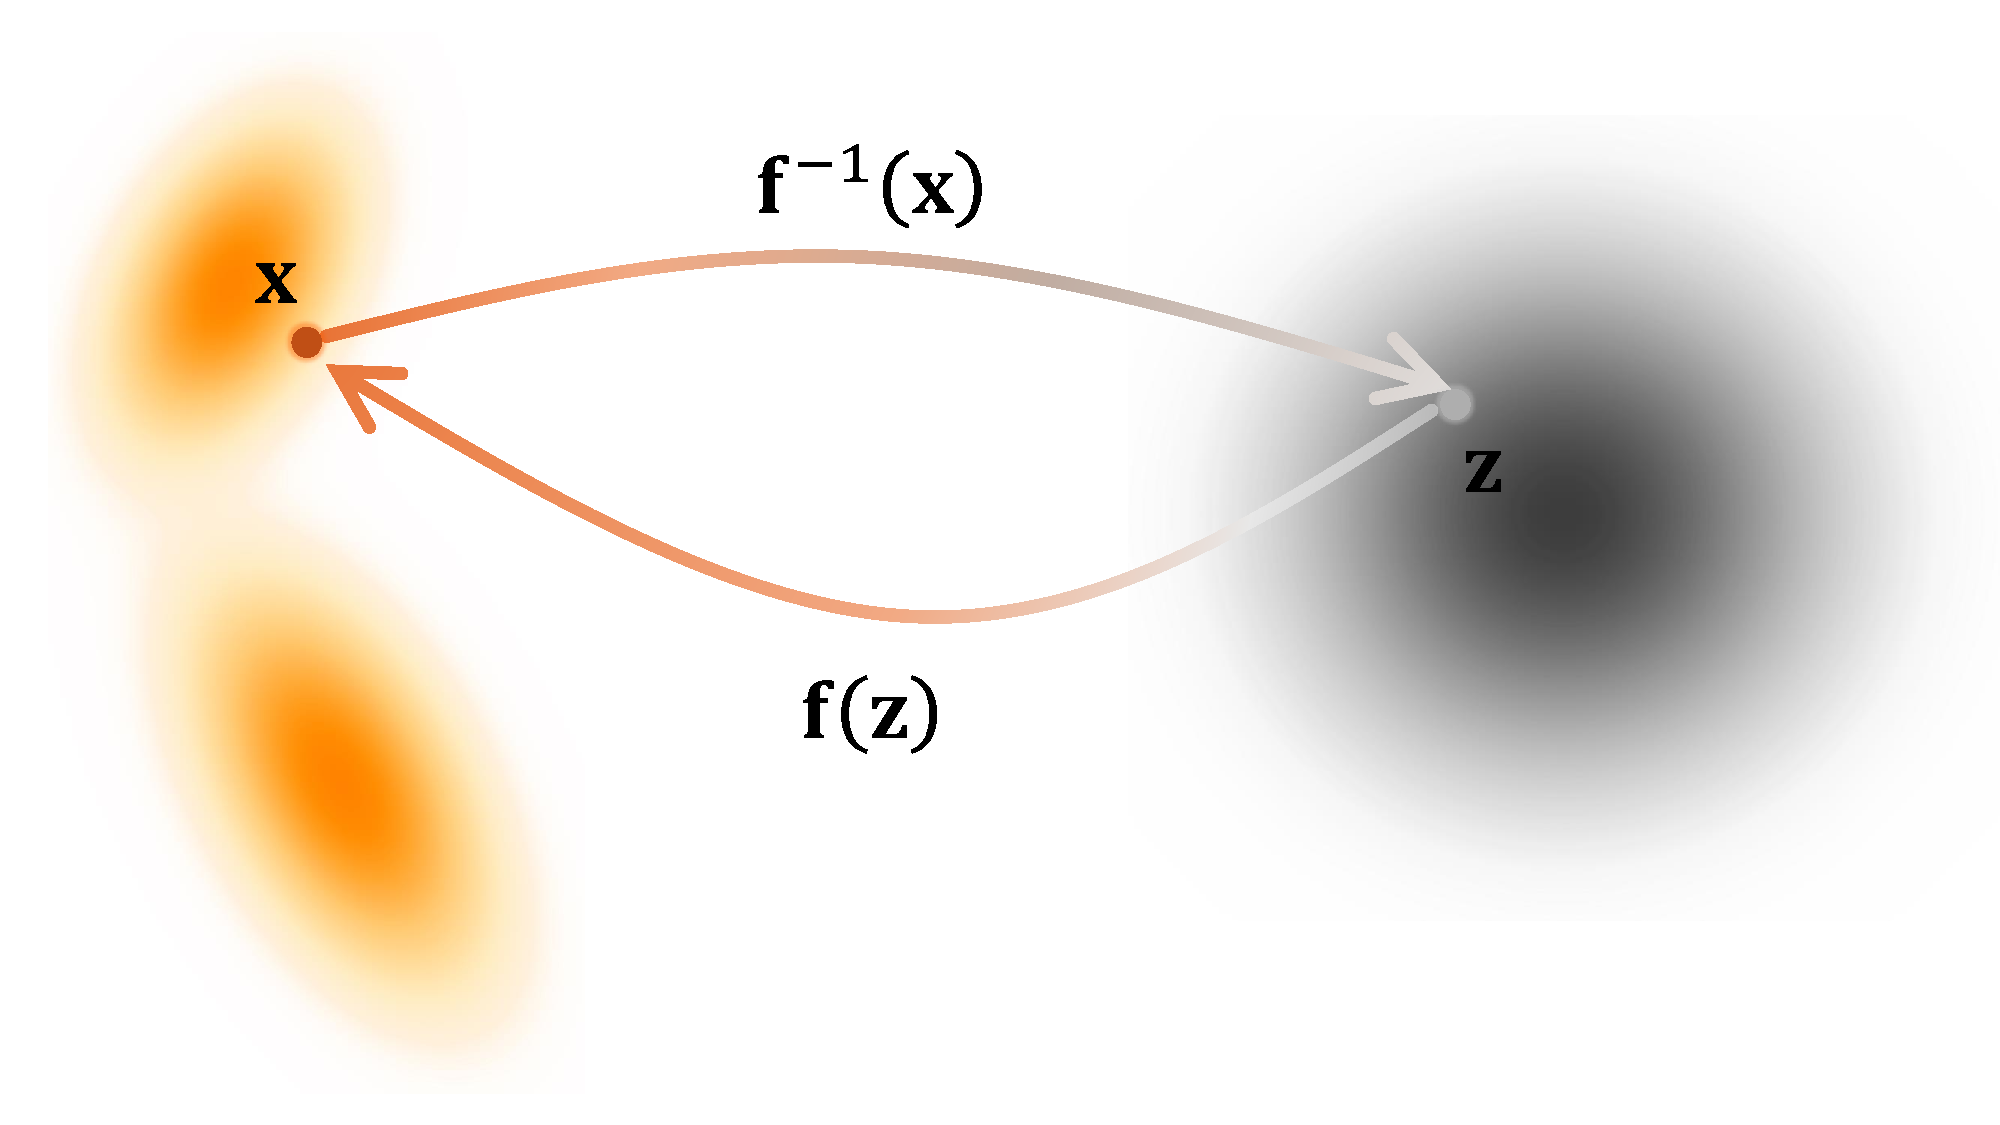
\includegraphics[width=0.9\linewidth]{Images/PartB/flow_density.pdf}
    \caption{\textbfs{可逆映射下 NF 的样本移动示意图。}它由一系列可逆函数 $\rvf: \rvz \mapsto \rvx$ 构成，这些函数将隐变量 $\rvz$ 变换为数据 $\rvx$，同时逆映射 $\rvf^{-1}: \rvx \mapsto \rvz$ 用于重建数据。一个 NF 类似于编码器--解码器结构，但编码器被实现为一个光滑可逆映射，而解码器恰为其逆映射。相应的密度变化可通过变量替换公式计算，如 \Cref{eq:nf-change-of-var} 所示。\figcredit{由作者绘制。}}
    \label{fig:sample-and-change-of-variable}
\end{figure}

\subsection{归一化流}

NF~\citep{rezende2015variational} 通过一个可逆映射将一个简单先验 $p_{\text{prior}}(\rvz)$（例如标准高斯 $\mathcal{N}(\bm{0}, \rmI)$）进行变换，来建模一个复杂数据分布 $p_{\text{data}}(\rvx)$：
\[
\rvf_{\bm{\phi}}: \mathbb{R}^D \to \mathbb{R}^D,
\]
其中 $\rvx = \rvf_{\bm{\phi}}(\rvz)$ 且 $\rvz \sim p_{\text{prior}}$。这里 $\rvx$ 与 $\rvz$ 维数相同。
利用 \Cref{eq:nf-change-of-var} 中的变量替换公式，模型似然为\footnote{若进一步约束该映射为某个凸势函数的梯度，
即 $\rvf_\bphi = \nabla \psi_\bphi$，其中 $\psi_\bphi$ 为凸函数，则
\Cref{eq:nf-change-of-var-log} 退化为 \Cref{eq:monge-ampere} 中的 Monge--Ampère
关系。
该偏微分方程刻画了在二次代价下从一个分布到另一个分布的最优变换。详见 \Cref{ch:ot-eot} 与 \citep{huangconvex}。
}
\begin{align}\label{eq:nf-change-of-var-log}
\log p_{\bm{\phi}}(\rvx) = \log p_{\text{prior}}(\rvz) + \log \left| \det \frac{\partial \rvf_{\bm{\phi}}^{-1}(\rvx)}{\partial \rvx} \right|.
\end{align}




\paragraph{训练目标。}
参数 $\bm{\phi}$ 通过在数据上最大化似然来学习：
\begin{align}\label{eq:nf-training}
\mathcal{L}_{\text{NF}}(\bm{\phi}) = \mathbb{E}_{\rvx \sim p_{\text{data}}} \left[ \log p_{\bm{\phi}}(\rvx) \right].
\end{align}
计算 \Cref{eq:nf-change-of-var-log} 中的雅可比行列式代价可能很高，一般情况下复杂度标度为 $\mathcal{O}(D^3)$。

\paragraph{构造可逆变换。}






单一复杂可逆网络因其雅可比行列式而代价高昂。反之，简单变换（例如线性变换）虽然高效，却缺乏表达能力。


为在二者之间取得平衡，NF 采用一串 $L$ 个可训练的可逆映射 $\{\rvf_k\}_{k=0}^{L-1}$，每个映射都具有可高效计算的雅可比：
\[
\rvf_{\bm{\phi}} = \rvf_{L-1} \circ \rvf_{L-2} \circ \cdots \circ \rvf_0.
\]
每个 $\rvf_k$ 都由一个神经网络参数化，但为简洁起见我们省略对 ${\bm{\phi}}$ 的显式依赖。


样本经如下方式变换：
\begin{align}\label{eq:nf-seq}
\rvx_{k+1} = \rvf_k(\rvx_k), \quad k = 0, \ldots, L-1,
\end{align}
其中 $\rvz=\rvx_0 \sim p_{\text{prior}}$ 且 $\rvx = \rvx_L$ 对应数据。所得的（对数）密度为
\begin{align}\label{eq:multi-nf-density}
\begin{aligned}
    p_{\bm{\phi}}(\rvx) &= p_{\text{prior}}(\rvx_0) \prod_{k=0}^{L-1} \left| \det \frac{\partial \rvf_k}{\partial \rvx_k} \right|^{-1}, \text{ or equivalently,}\\
\log p_{\bm{\phi}}(\rvx) &= \log p_{\text{prior}}(\rvx_0) + \sum_{k=0}^{L-1} \log \left| \det \frac{\partial \rvf_k}{\partial \rvx_k} \right|^{-1}.
\end{aligned}
\end{align}


\vspace{0.3cm}
\begin{figure}[tbh!]
    \centering
\begin{tikzpicture}[
    ->, % Sets default arrow type
    >=Stealth, % Sets default arrowhead style
    node_dist/.style={left=1.7cm of #1}, % Position nodes to the LEFT
    font=\small,
    thick
  ]

  % Define a style for the nodes
  \tikzset{state/.style={
      rectangle,
      rounded corners=3pt,
      draw=black,
      fill=gray!10,
      minimum height=35pt,
      minimum width=25pt
    }
  }

  % Place the nodes from RIGHT to LEFT
  \node[state] (x0) {$\rvx_0 $};
  \node[state] (x1) [node_dist=x0] {$\rvx_1$};
  \node[state] (x2) [node_dist=x1] {$\rvx_2$};
  \node (dots) [left=0.7cm of x2] {$\boldsymbol{\cdots}$};
  \node[state] (xL) [node_dist=dots] {$\rvx_L$};

  % Draw the arrows (edges) with labels
  
  % Top path (Generative, right to left) - Shifted up
  \path [black] ([yshift=4.5pt]x0.west)  edge node[above] {$\rvf_0$} ([yshift=4.5pt]x1.east);
  \path [black] ([yshift=4.5pt]x1.west) edge node[above] {$\rvf_1$} ([yshift=4.5pt]x2.east);
  \path [black] ([yshift=4.5pt]x2.west) edge ([yshift=4.5pt]dots.east);
  \path [black] ([yshift=4.5pt]dots.west) edge node[above, pos=0.4] {$\rvf_{L-1}$} ([yshift=4.5pt]xL.east);
  
  % Bottom path (Inference, left to right) - Shifted down
  \path ([yshift=-4.5pt]x1.east) edge node[below] {$\rvf_0^{-1}$} ([yshift=-4.5pt]x0.west);
  \path ([yshift=-4.5pt]x2.east) edge node[below] {$\rvf_1^{-1}$} ([yshift=-4.5pt]x1.west);
  \path ([yshift=-4.5pt]dots.east) edge ([yshift=-4.5pt]x2.west);
  \path ([yshift=-4.5pt]xL.east) edge node[below, pos=0.6] {$\rvf_{L-1}^{-1}$} ([yshift=-4.5pt]dots.west);

\end{tikzpicture}
\caption{\textbfs{NF 示意图。}一个 NF 由一叠可逆映射
$\rvf_{\bm{\phi}} = \rvf_{L-1} \circ \rvf_{L-2} \circ \cdots \circ \rvf_0$ 构成。
该变换将隐变量样本 $\rvx_0 \sim p_{\mathrm{prior}}$ 映射为数据样本 $\rvx_L \sim p_{\mathrm{data}}$。\figcredit{由作者绘制。}}
    \label{fig:nf-stack}
\end{figure}

\paragraph{可逆流的示例。}已有大量文献聚焦于设计能够高效计算雅可比行列式的单层流构造。下面我们介绍两种具有代表性的类型：平面流~\citep{rezende2015variational} 与残差流~\citep{chen2019residual,behrmann2019invertible}，后者启发了 \Cref{subsec:NODE} 中的发展。
\subparagraph{平面流：}它施加一个简单的变换
\[
\rvf(\rvz) = \rvz + \rvu h(\rvw^\top \rvz + b),
\]
where $\rvu, \rvw \in \mathbb{R}^D$，$b \in \mathbb{R}$，$h(\cdot)$ 是一个激活函数。雅可比行列式为
\[
\left| 1 + \rvu^\top h'(\rvw^\top \rvz + b) \rvw \right|.
\]

\subparagraph{残差流：}
将变换 $\rvf$ 定义为
\begin{align}\label{eq:residual-flow}
\rvf(\rvz) = \rvz + \rvv(\rvz),
\end{align}
其中 $\rvv$ 为压缩映射（Lipschitz 常数 $< 1$）。这由 Banach 不动点定理保证了可逆性。

雅可比的对数行列式可化简为迹展开：
\begin{align}\label{eq:log-det-tr}
    \log \Bigg|\det \frac{\partial \rvf(\rvz)}{\partial \rvz} \Bigg| &= \log \left( \det \frac{\partial \rvf(\rvz)}{\partial \rvz} \right) \nonumber\\
    &= \Tr\left(\log\left(\frac{\partial \rvf(\rvz)}{\partial \rvz}\right)\right) \nonumber\\
    &= \Tr\left(\log\left(\rmI + \frac{\partial \rvv(\rvz)}{\partial \rvz}\right)\right) \nonumber\\
    &= \sum_{k=1}^{\infty} \frac{(-1)^{k+1}}{k} \Tr\left(\left(\frac{\partial \rvv(\rvz)}{\partial \rvz}\right)^k\right),
\end{align}
借助于迹估计量~\citep{hutchinson1989stochastic} 可使计算变得高效。

\paragraph{采样与推断。}
从 NF 中采样非常直接：抽取 $\rvx_0 \sim p_{\text{prior}}$ 并计算 $\rvx = \rvf_{\bm{\phi}}(\rvx_0)$。精确似然可由 \Cref{eq:multi-nf-density} 得到。


\subsection{神经 ODE}\label{subsec:NODE}
\begin{figure}[th!]
    \centering
    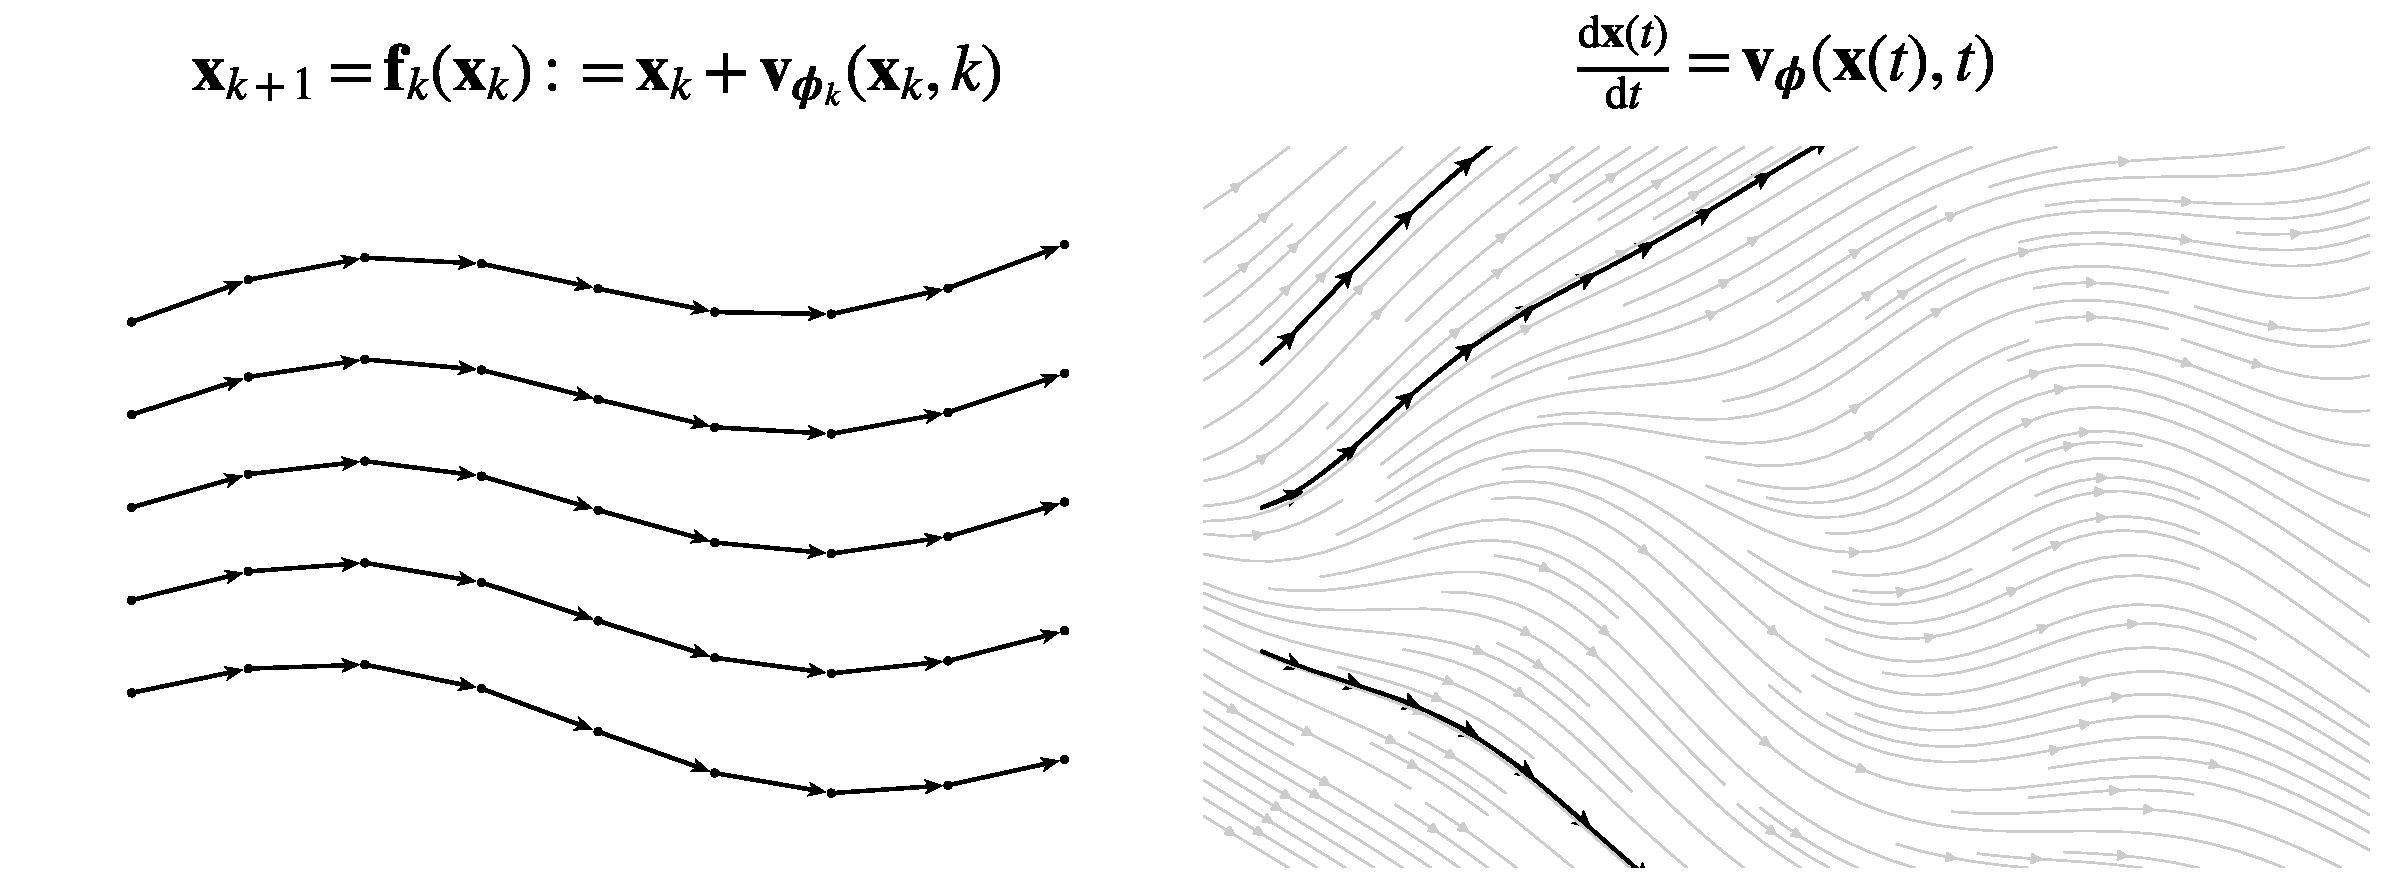
\includegraphics[width=\linewidth]{Images/PartB/discrete_vs_continuous_side_by_side_white.pdf}
    \caption{\textbfs{离散时间与连续时间归一化流的对比。}（左）一个离散 NF 通过有限序列的可逆映射 $\mathbf{x}_{k+1} = \mathbf{f}_k(\mathbf{x}_k)$ 传输样本，
得到分段、不相交的轨迹（带箭头的点）。（右）一个连续 NF（神经 ODE）沿 $\frac{\diff\mathbf{x}(t)}{\diff t} = \mathbf{v}_{\boldsymbol{\phi}}(\mathbf{x}(t),t)$ 的积分曲线演化状态，
其中带切向箭头的黑色路径绘制在灰色向量场之上。\figcredit{由作者绘制。}}
    \label{fig:nf-cnf}
\end{figure}


\paragraph{从离散时间 NF 到连续时间 NF（神经 ODE）。}
NF 通常被表述为一串 $L$ 个离散、可逆的变换。透过 \Cref{eq:nf-seq} 以及 \Cref{eq:residual-flow} 中“残差流”形式的视角，每一层可写成如下形式：
\[
\rvx_{k+1} = \rvf_k(\rvx_k) := \rvx_k + \rvv_{\bm{\phi}_k}(\rvx_k, k),
\]
where $\rvv_{\bm{\phi}_k}(\cdot, k)$ 是一个由神经网络参数化的、与层相关的速度场。直观地讲，这个速度场是一个学习到的向量值函数，它以平滑的小步幅在输入空间中“推动”数据点。每次变换都沿着该速度所提示的方向移动点，逐步将简单的先验分布塑造为复杂的目标分布。


事实上，这一表述恰好对应于带可学习参数 $\bphi$ 的连续时间 ODE 的 Euler 离散化：
\[
\frac{\diff \rvx(t)}{\diff t} = \rvv_{\bm{\phi}}(\rvx(t), t).
\]
 在层数趋于无穷、步长趋于零（$\Delta t \to 0$）的极限下，离散 NF 收敛到一个连续模型，由此得到 \emph{神经 ODE}（NODE）~\citep{chen2018neural} 的框架，也称为 \emph{连续归一化流}（CNF）。



\paragraph{神经 ODE 的形式化设定。}
一个神经 ODE 通过下式定义一个连续变换：
\begin{align}\label{eq:neural-ode}
    \frac{\diff \rvx(t)}{\diff t} = \rvv_{\bm{\phi}}(\rvx(t), t),\quad t\in [0,T]
\end{align}
where:
\begin{itemize}
    \item $ \rvx(t) \in \mathbb{R}^D $ 是 $t$ 时刻的状态；为简洁起见，我们有时写作 $\rvx_t$；
    \item $\rvv_{\bm{\phi}}(\rvx(t), t)$ 是由 $\bm{\phi}$ 参数化的神经网络。
\end{itemize}


\subparagraph{NODE 的目标。}
从初始条件 $\rvx(0) \sim p_{\text{prior}}$ 出发，ODE 随时间连续演化状态，诱导出一族边际分布 $p_{\bm{\phi}}(\rvx_t, t)$（与 PF-ODE 类似！）\footnote{我们采用翻转时间的约定：$t = 0$ 表示先验（源），$t = 1$ 表示数据（目标）分布。先验可交替地写作 $p_{\bm{\phi}}(\rvx(0), 0)$、$p_{\text{prior}}(\rvx(0), 0)$，或简写为 $p_{\text{prior}}(\rvz)$。
}。

目标是学习神经向量场 $\rvv_{\bm{\phi}}$，直观上它表示一个沿数据空间中连续轨迹传输点的速度。通过学习这一速度，$t=T$ 时刻的终端分布将匹配目标分布 $p_{\mathrm{data}}(\cdot)$。这一连续变换将离散归一化流和神经 ODE 统一在同一个框架之中。


\begin{figure}
    \centering
    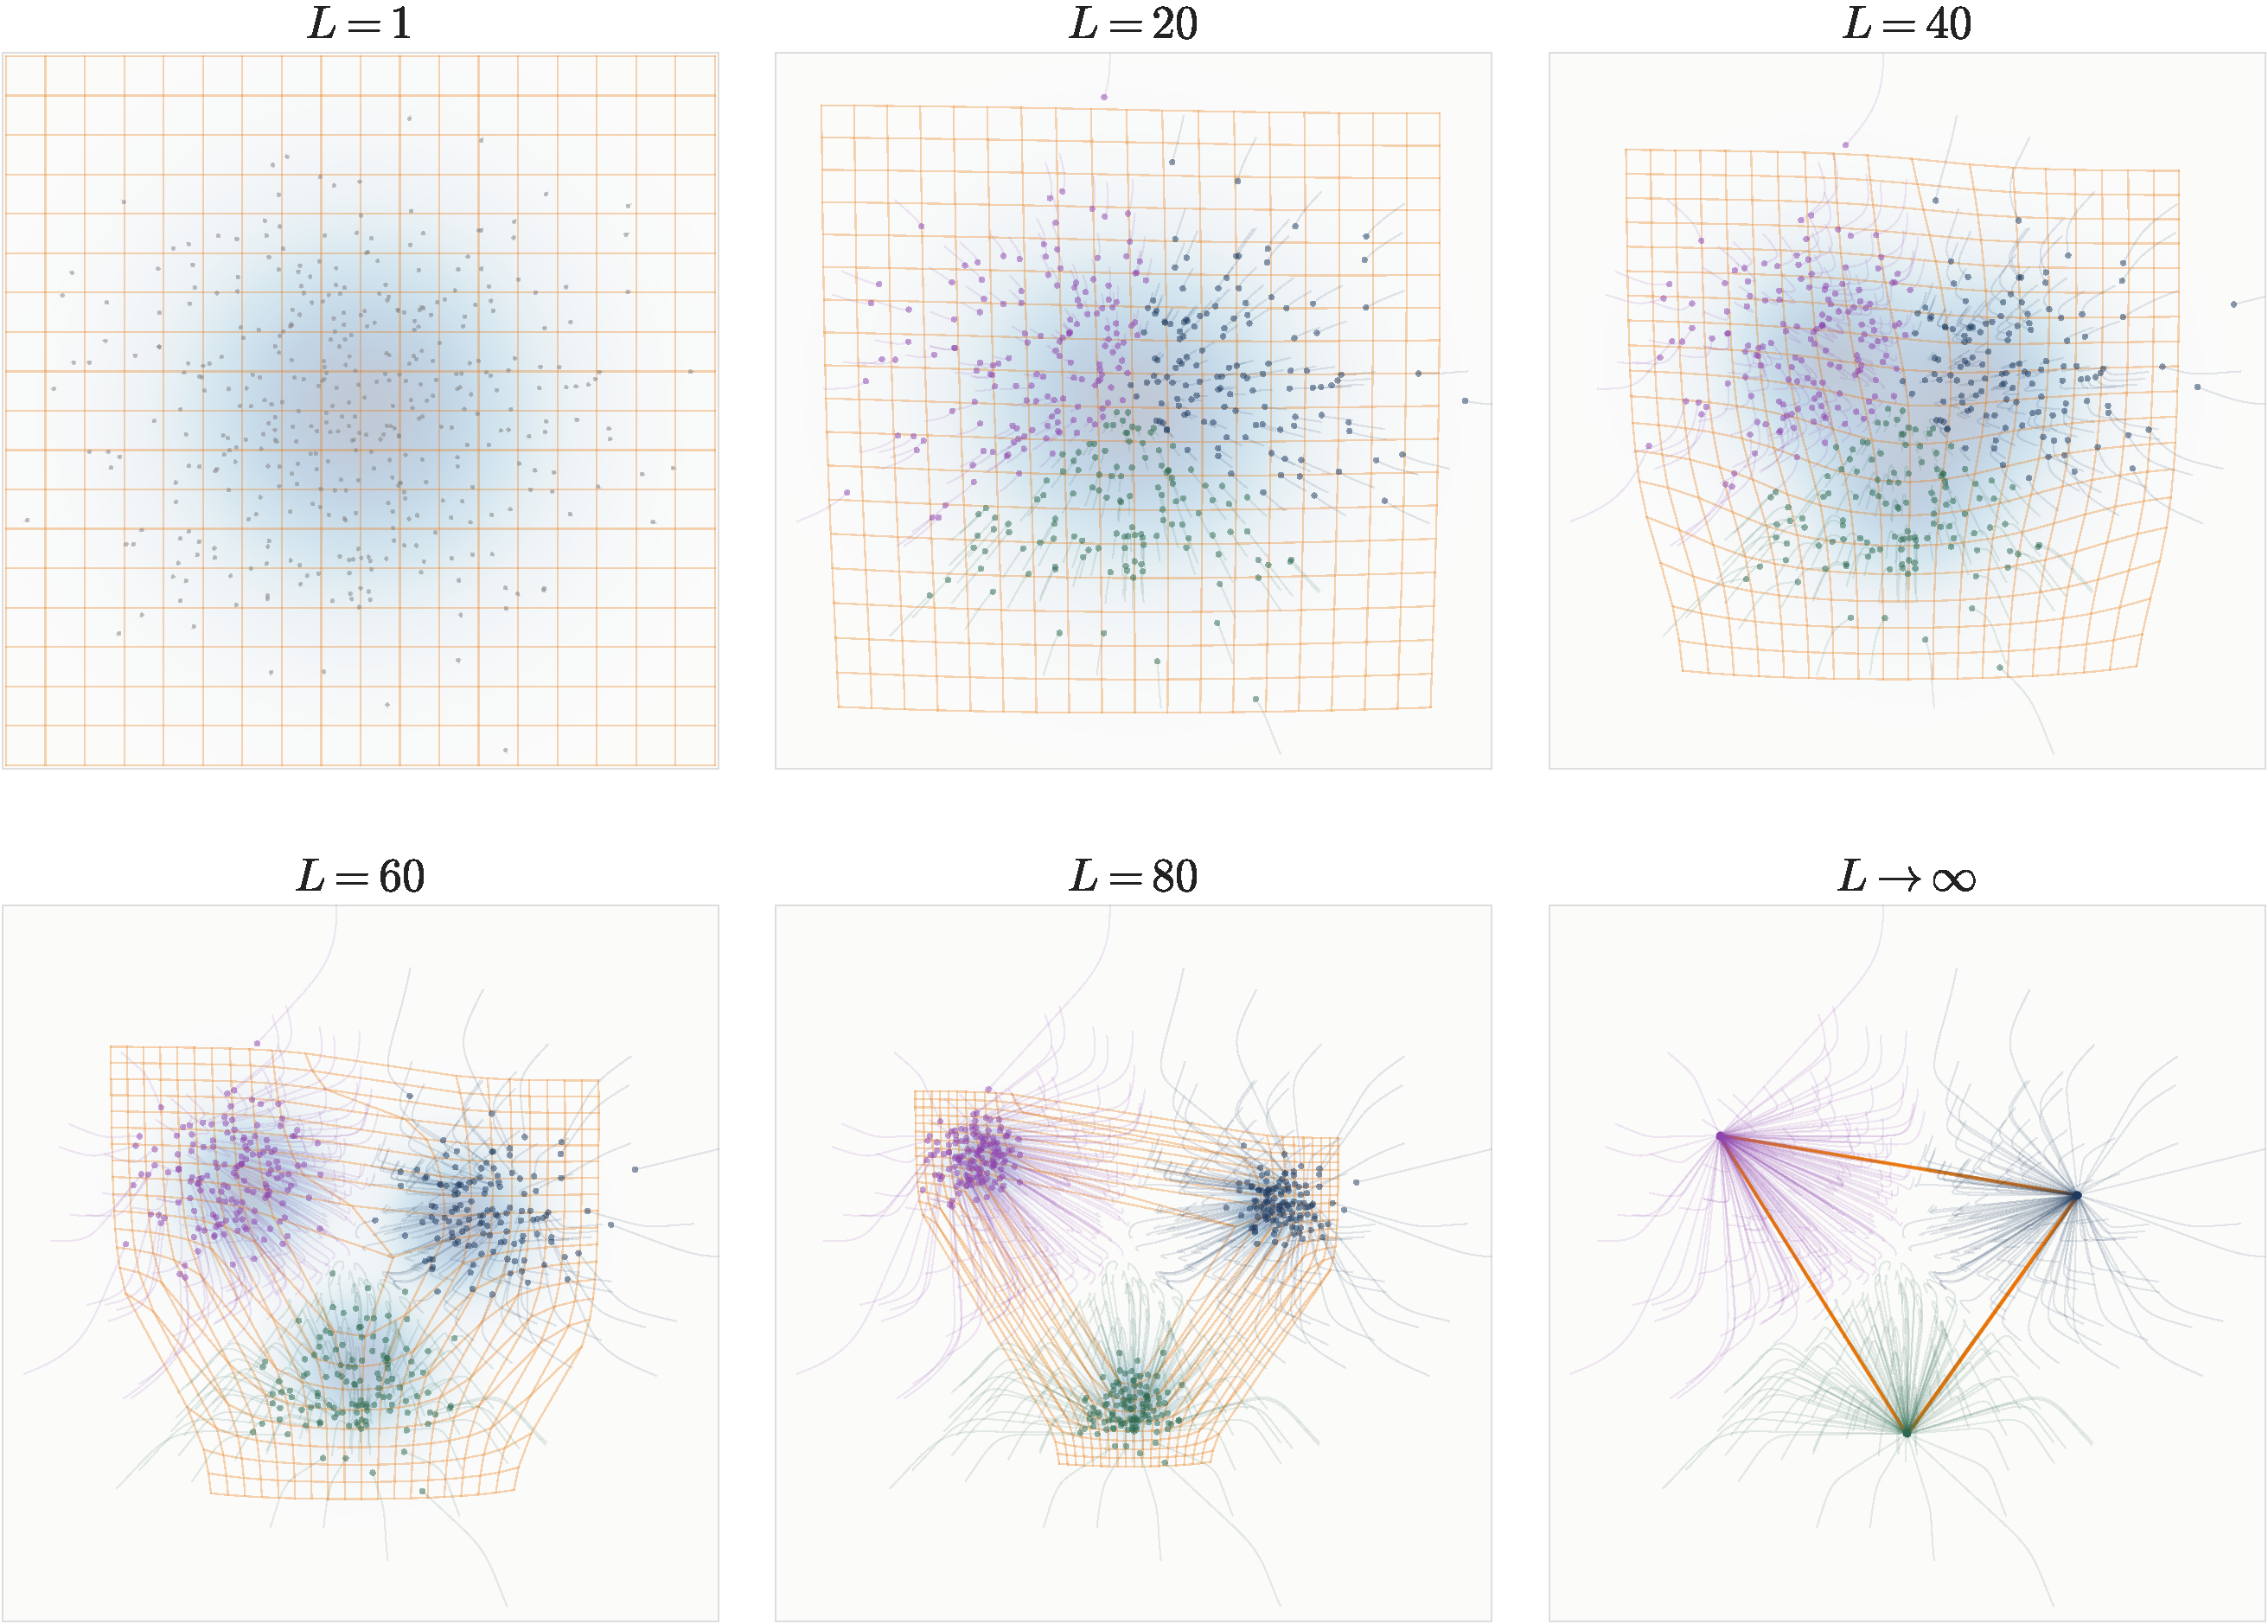
\includegraphics[width=\linewidth]{Images/PartB/cov_2d_layers.pdf}
    \caption{\textbfs{逼近一个连续传输流的离散双射。}
随着双射层数 $L$ 增加，映射复合逐步使样本、潜在分布以及参考网格从源配置变形到目标几何。
当 $L$ 较小时，变换较为粗糙、明显分层；随着 $L$ 增大，变形变得更加平滑、分辨率更高。
在无穷深度的极限下，若按每一层成为一个无穷小变换的标度进行缩放，则堆叠的双射逼近一个连续的、依赖时间的流，所诱导的密度演化由 \Cref{eq:continuity_eq} 中的连续性方程主宰。\figcredit{由作者在 AI 辅助编程下绘制。}}
    \label{fig:bijection-continuity}
\end{figure}



\paragraph{连续时间的变量替换公式。}
类似于 \Cref{eq:nf-change-of-var} 或 \Cref{eq:multi-nf-density}，\citet{chen2018neural} 推导出了变量替换公式的连续时间类比。对于在 \Cref{eq:neural-ode} 下演化的过程 $\rvx(t)$，其依赖于时间的密度 $p_{\bm{\phi}}(\rvx(t), t)$，所谓的 \emph{瞬时变量替换公式} 为：
\[
\frac{\diff}{\diff t} \log p_{\bm{\phi}}(\rvx(t), t) = -\nabla_{\rvx}\cdot\rvv_{\bm{\phi}}(\rvx(t), t).
\]
因此，在给定先验 $p_{\text{prior}}(\rvx(T), T)$ 下，由神经 ODE 诱导的终端状态 $\rvx(T)$ 的对数密度为
\begin{align}\label{eq:NODE-likelihood}
    \log p_{\bm{\phi}}(\rvx(T), T) = \log p_{\text{prior}}(\rvx(0), 0) - \int_0^T \nabla_{\rvx} \cdot \rvv_{\bm{\phi}}(\rvx(t), t)   \mathrm{d}t.
\end{align}
该表达式通过数值求解 ODE 即可实现精确似然计算，进而允许对模型进行最大似然训练。我们稍后将对此详细展开。


尽管初看可能陌生，这个瞬时变量替换公式其实是 Fokker-Planck 方程的一个特例，具体而言是其确定性形式，即所谓的 \emph{连续性方程}（见 \Cref{app:continuity}）。它也可被解释为 \Cref{eq:multi-nf-density} 的连续时间极限。我们将这一结果及其推导总结为如下引理：

\lemp{瞬时变量替换}{instant-change-of-var}{
设 ${\rvz}(t)$ 是一个具有依赖时间的密度 $p({\rvz}(t), t)$ 的连续随机过程，且假设它按如下 ODE 演化：
\begin{align*}
    \frac{\diff \rvz(t)}{\diff t} = \mathbf{F}({\rvz}(t), t).
\end{align*}
假设 $\mathbf{F}$ 在 ${\rvz}$ 上一致 Lipschitz 且关于 $t$ 连续，则对数密度的时间导数满足：
\begin{align}\label{eq:instant-change-of-var}
\frac{\partial \log p({\rvz}(t), t)}{\partial t} = -\nabla_\rvz \cdot \mathbf{F} (\rvz(t), t).
\end{align}
}{我们在 \Cref{app-sec:flow-proof} 中给出两种等价的推导。
}


\subparagraph{与离散时间公式的联系。}
\Cref{eq:NODE-likelihood} 中 NODE 的似然，
\[
\log p_{\bm{\phi}}(\rvx(T), T) = \log p_{\text{prior}}(\rvx(0), 0) - \int_0^T \nabla_\rvx \cdot \rvv_{\bm{\phi}}(\rvx(t), t) \diff t,
\]
可以被视为 \Cref{eq:multi-nf-density} 中离散归一化流公式的连续时间类比：
\[
\log p_{\bm{\phi}}(\rvx_L) = \log p_{\text{prior}}(\rvx_0) - \sum_{k=0}^{L-1} \log \left| \det \frac{\partial \rvf_k}{\partial \rvx_k} \right|.
\]
积分对应于求和，迹算子则取代了对数行列式，正如 \Cref{eq:log-det-tr} 中所讨论的那样。这些对应关系在引理的证明中得到了进一步探讨。

\paragraph{训练 NODE。}
基于 \Cref{eq:NODE-likelihood}，NODE 学习一个参数化的速度场 $\rvv_{\bm{\phi}}$，使得终端分布
\[
p_{\bm{\phi}}(\cdot, T) \approx p_{\text{data}},
\]
其中轨迹从隐变量 $\rvx(0) \sim p_{\text{prior}}$ 出发，经 ODE 流演化。训练遵循 \Cref{eq:MLE} 中的 MLE 框架：
\[
\mathcal{L}_{\text{NODE}}(\bm{\phi}) := \mathbb{E}_{\rvx \sim p_{\text{data}}} \big[\log p_{\bm{\phi}}(\rvx, T)\big].
\]

\subparagraph{精确对数似然计算。}
为了计算数据点 $\mathbf{x}$ 的 $\log p_{\bm{\phi}}(\mathbf{x}, T)$，我们对变量替换公式 \eqref{eq:NODE-likelihood} 进行积分：
\begin{align}
\log p_{\bm{\phi}}(\mathbf{x}, T) = \log p_{\text{prior}}(\mathbf{z}(0)) - \int_0^T \nabla_{\mathbf{z}} \cdot \mathbf{v}_{\bm{\phi}}(\mathbf{z}(t), t) \diff t.
\end{align}
这里 $\mathbf{z}(t)$ 从 $t = T$ 反向求解到 $t = 0$ 的 ODE：
\[
\frac{\diff\mathbf{z}}{\diff t} = \mathbf{v}_{\bm{\phi}}(\mathbf{z}(t), t)
\]
初值取 $\mathbf{z}(T) = \mathbf{x}$。对标准分布而言，先验项 $\log p_{\text{prior}}(\mathbf{z}(0))$ 是易处理的。这使得神经 ODE 中可以进行精确的、基于似然的训练与评估。

\subparagraph{基于梯度的优化。}
最大化 $\mathcal{L}_{\text{NODE}}$ 需要通过 ODE 求解器进行反向传播。伴随灵敏度方法~\citep{pontryagin2018mathematical, chen2018neural} 通过一个辅助 ODE 来计算梯度，具有 $\mathcal{O}(1)$ 的内存复杂度，但由于每一步都需要数值积分，NODE 的训练仍然代价高昂。

\paragraph{用 NODE 进行推断。}
用训练好的模型 $\rvv_{\bm{\phi}^\times}$ 进行采样，需抽取 $\rvx(0) \sim p_{\text{prior}}$ 并向前积分（借助数值求解器）：
\[
\rvx(T) = \rvx(0) + \int_0^T \rvv_{\bm{\phi}^\times}(\rvx(t), t)   \diff t.
\]
终端状态 $\rvx(T)$ 近似为来自 $p_{\text{data}}$ 的一个样本。

此外，我们注意到对于任意向量场 $\rmF$，下述恒等式成立：
\[
    \Tr\left(\frac{\partial \rmF}{\partial \rvz(t)} \right) = \nabla_{\rvz} \cdot \rmF.
\]
因此，散度可以借助随机迹估计量（例如 Hutchinson 估计量~\citep{hutchinson1989stochastic}）进行高效估计，这使得在高维情形下精确似然计算变得更加可行。


% \subsection{Closing Remarks}\label{subsec:remark-flow}
%  We first compare NODEs with discrete NFs, then outline their connection to diffusion models.
% \paragraph{Advantages of NODEs over Discrete NFs.}
% NODEs offer two key advantages:
% \begin{enumerate}
%     \item \textbfs{Flexible Architectures:} Unlike discrete NFs, NODEs do not require invertible transformations, as ODE solutions are guaranteed under Lipschitz conditions on the velocity field $\rvv_{\bm{\phi}}$.
%     \item \textbfs{Efficient Likelihoods Computation:} NODEs compute divergence $\nabla \cdot \rvv_{\bm{\phi}}$ with $\mathcal{O}(D)$ complexity, compared to the $\mathcal{O}(D^3)$ Jacobian determinant in discrete NFs, enabling high-dimensional scalability.
% \end{enumerate}
% Beyond generative modeling, NODEs are also used in dynamical systems, time series, and mathematical physics~\citep{kidger2022neural}.


% \paragraph{What Lies Ahead?}
% In this section, we have examined the development of NFs and NODEs:
% \begin{itemize}
%     \item \textbfs{Stage 1.} Single-layer invertible transformations in NFs;
%     \item \textbfs{Stage 2.} Multiple layers of invertible transformations in NFs;
%     \item \textbfs{Stage 3.} Continuous-time extension through NODEs, equivalent to infinitely many layers of invertible transformations.
% \end{itemize}

% It is fascinating to see how the evolution of flow-based models echoes that of VAEs~(\Cref{ch:variational}) and score-based methods~(\Cref{ch:score-based}). Each of these modeling paradigms embarks on a similar journey: beginning with simple, discrete-time, single-layer structures, advancing to deeper multi-layer designs (e.g., DDPM/NCSN), and ultimately converging toward elegant continuous-time formulations (Score SDE).

% However, a crucial difference emerges: even though diffusion models are associated with an ODE (i.e., PF-ODE), they do not directly learn an arbitrary velocity field $\mathbf{v}_{\bm{\phi}}$ as in NODEs. Instead, diffusion models learn objectives (e.g., score) that define ODEs aimed at matching prescribed marginal distributions--governed by Fokker-Planck equation. This approach makes diffusion model training simulation-free and thus computationally efficient, in contrast to NODEs which require solving numerical ODEs during training.

% Flow matching inherits this essential characteristic of diffusion model training and resolves the simulation bottleneck of NODEs, enabling efficient distribution-to-distribution transport via ODEs with prescribed underlying structure. We will explore this further in the next chapter.




\newpage
\clearpage
\section{\texorpdfstring{流匹配框架}{Flow Matching Framework}}\label{sec:flow-matching-framework}

Score SDE~（\Cref{ch:score-sde}）与 NODE~（\Cref{sec:flow-based-method}）为生成建模提供了一种替代视角：学习一个连续时间的流（随机或确定），将一个简单的高斯先验样本 $\bm{\epsilon} \sim p_{\text{prior}}$ 传输为来自 $p_{\text{data}}$ 的类数据样本。

\emph{流匹配}（FM）框架~\citep{lipman2022flow,lipman2024flow,tongimproving} 在这一思想之上展开，并将其推广为学习两个 \emph{任意} 固定端点分布之间的流：一个源分布 $p_{\text{src}}$ 和一个目标分布 $p_{\text{tgt}}$，并假定二者都易于采样。在这一更宽泛的设定中，生成任务成为 $p_{\text{src}}$ 为高斯先验、$p_{\text{tgt}}$ 为数据分布时的特例。

本节我们采用 FM 的视角\footnote{若干相关方法都共享用连续时间流在端点分布之间进行传输这一核心思想，只是表述略有不同。这些方法包括流匹配（FM）~\citep{lipman2022flow,neklyudov2023action}、整流流（RF）~\citep{liu2022rectified,heitz2023iterative} 和随机插值~\citep{albergo2023stochastic,albergobuilding,ma2024sit}。这里我们采用 FM 的术语作为一种统一的表示。}，强调其核心原理：学习一个依赖时间的向量场 $\mathbf{v}_t(\rvx_t)$，使与之对应的 ODE 流在满足边界条件
\[
p_0 = p_{\text{src}}, \quad p_1 = p_{\text{tgt}}.
\]
When $p_{\text{src}}$ 为高斯分布时，我们称这一设定为 \emph{高斯流匹配}。与经典扩散模型相比，FM 仅利用端点处的样本即可实现针对一大类传输问题的高效、免仿真训练。






\subsection{来自基于分数方法的启示}\label{subsec:lesson-score}

我们用一种略有不同但等价的表述重新审视 Score SDE 框架（\Cref{ch:score-sde}），从中提炼出激发 FM 方法的关键见解。这一分析揭示了扩散模型如何隐式地学习概率流，并启发了更直接的表述形式。


\paragraph{第一步：定义条件路径及其边际密度。}

\begin{figure}[th!]
    \centering
    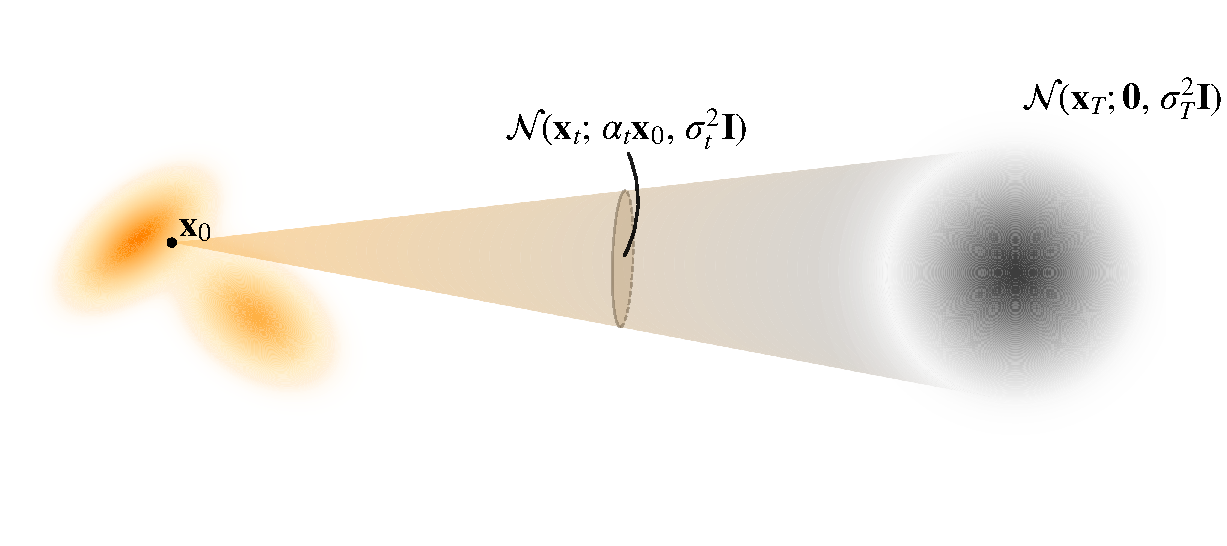
\includegraphics[width=\linewidth]{Images/PartB/data_vs_prior_cone_with_oval.pdf}
    % \vspace{-1.5cm}
    \caption{\textbfs{条件转移分布示意图。}
$p_t(\rvx_t | \rvx_0) = \mathcal{N}(\rvx_t;\alpha_t \rvx_0,\sigma_t^2 \mathbf{I})$，
定义了一条（高斯）条件概率路径，从数据样本
$\rvx_0 \sim p_{\text{data}}$（左）通向高斯先验
$p_{\text{prior}}$（右）。\figcredit{由作者绘制。}}
    \label{fig:data-prior-conditioning}
\end{figure}

一个扩散模型指定了一个连续时间的密度族 $\{p_t\}_{t \in [0,1]}$，它在 $t=1$ 处将一个简单先验 $p_{\text{prior}}$（例如高斯）作为源，传输到 $t=0$ 处的目标数据分布 $p_{\text{data}}$：
\[
p_1(\rvx_1) = p_{\text{prior}}(\rvx_1), \quad p_0(\rvx_0) = p_{\text{data}}(\rvx_0).
\]
该路径通过前向条件分布隐式定义：
\begin{align}\label{eq:lesson-dm-conditional-path}
    p_t(\rvx_t|\rvx_0) = \mathcal{N}(\rvx_t; \alpha_t \rvx_0, \sigma_t^2 \mathbf{I}), \quad \rvx_0\sim p_{\text{data}}
\end{align}
它诱导出边际密度
\[
p_t(\rvx_t) := \int p_t(\rvx_t |\rvx_0)  p_{\text{data}}(\rvx_0) \mathrm{d}\rvx_0.
\]
条件高斯方差 $\sigma_t^2$ 的增长驱动 $p_t$ 向高斯先验演化。

\paragraph{第二步：速度场。}
边际密度 $p_t$ 的时间演化由一个速度场 $\rvv_t : \mathbb{R}^D \to \mathbb{R}^D$ 主宰，它由 Fokker-Planck 方程导出：
\begin{align}\label{eq:dm-velocity}
    \rvv_t(\rvx) := f(t)\rvx - \frac{1}{2}g^2(t)\nabla_{\rvx} \log p_t(\rvx),
\end{align}
which defines a deterministic particle flow through the PF-ODE:
\[
\frac{\diff \rvx(t)}{\diff t} = \underbrace{f(t)\rvx(t) - \frac{1}{2}g^2(t)\nabla_{\rvx} \log p_t\big(\rvx(t)\big)}_{\rvv_t(\rvx(t))}.
\]
该 ODE 将初始随机变量 $\rvx(0) \sim p_{\text{data}}$ 在时间上向前传输，或将 $\rvx(1) \sim p_{\text{prior}}$ 在时间上向后传输，使得 $\rvx(t)$ 的演化边际密度在每一个 $t \in [0,1]$ 上都匹配 $p_t$（见下文“底层规则”）。

标量函数 $f(t)$ 和 $g(t)$ 由相应前向 SDE 的系数决定，或者等价地由条件路径中定义的高斯核参数 $\alpha_t$ 和 $\sigma_t$ 决定（见 Lemma~\ref{forward-sde}）。


\paragraph{第三步：通过条件策略进行学习。}
目标是用一个神经网络 $\rvs_{\bm{\phi}}(\rvx_t, t)$ 来逼近神谕速度场 $\rvv_t(\rvx_t)$，训练目标为期望平方误差：
\[
\mathcal{L}_{\text{SM}}({\bm{\phi}}) = \mathbb{E}_{t \sim \mathcal{U}[0,1],  \rvx_t \sim p_t} \left[ \left\| \rvs_{\bm{\phi}}(\rvx_t, t) - \nabla_{\rvx_t} \log p_t(\rvx_t) \right\|^2 \right].
\]
由于边际分数 $\nabla_{\rvx_t} \log p_t(\rvx_t)$ 不可获取，我们利用易处理的条件分布来定义条件速度：
\[
\rvv_t(\rvx_t|\rvx_0) := f(t)\rvx_t - \frac{1}{2}g^2(t) \nabla_{\rvx_t} \log p_t(\rvx_t|\rvx_0).
\]
由全期望公式，边际分数可恢复为
\begin{align}\label{eq:marginal-oracle-score}
    \nabla_{\rvx_t} \log p_t(\rvx_t) = \mathbb{E}_{\rvx_0 \sim p(\cdot| \rvx_t)} \left[ \nabla_{\rvx_t} \log p_t(\rvx_t|\rvx_0) \right].
\end{align}
这为如下的替代训练目标提供了依据：
\[
\mathcal{L}_{\text{SM}}({\bm{\phi}}) = \underbrace{\mathbb{E}_{t,  \rvx_0 \sim p_{\text{data}},  \rvx_t \sim p_t(\cdot|\rvx_0)} \left[ \left\| \rvs_{\bm{\phi}}(\rvx_t, t) - \nabla_{\rvx_t} \log p_t(\rvx_t|\rvx_0) \right\|^2 \right]}_{\mathcal{L}_{\text{DSM}}({\bm{\phi}})} + C,
\]
其中 $C$ 是与 ${\bm{\phi}}$ 无关的常数。最小化子 $\rvs^*(\rvx_t, t)$ 满足
\[
\rvs^*(\rvx_t, t) = \mathbb{E}_{\rvx_0 \sim p(\cdot| \rvx_t)} \left[ \nabla_{\rvx_t} \log p_t(\rvx_t|\rvx_0) \right] = \nabla_{\rvx_t} \log p_t(\rvx_t),
\]
其中第二个等号由 \Cref{eq:marginal-oracle-score} 得到，从而验证了条件训练目标的正确性。

\begin{figure}
    \centering
    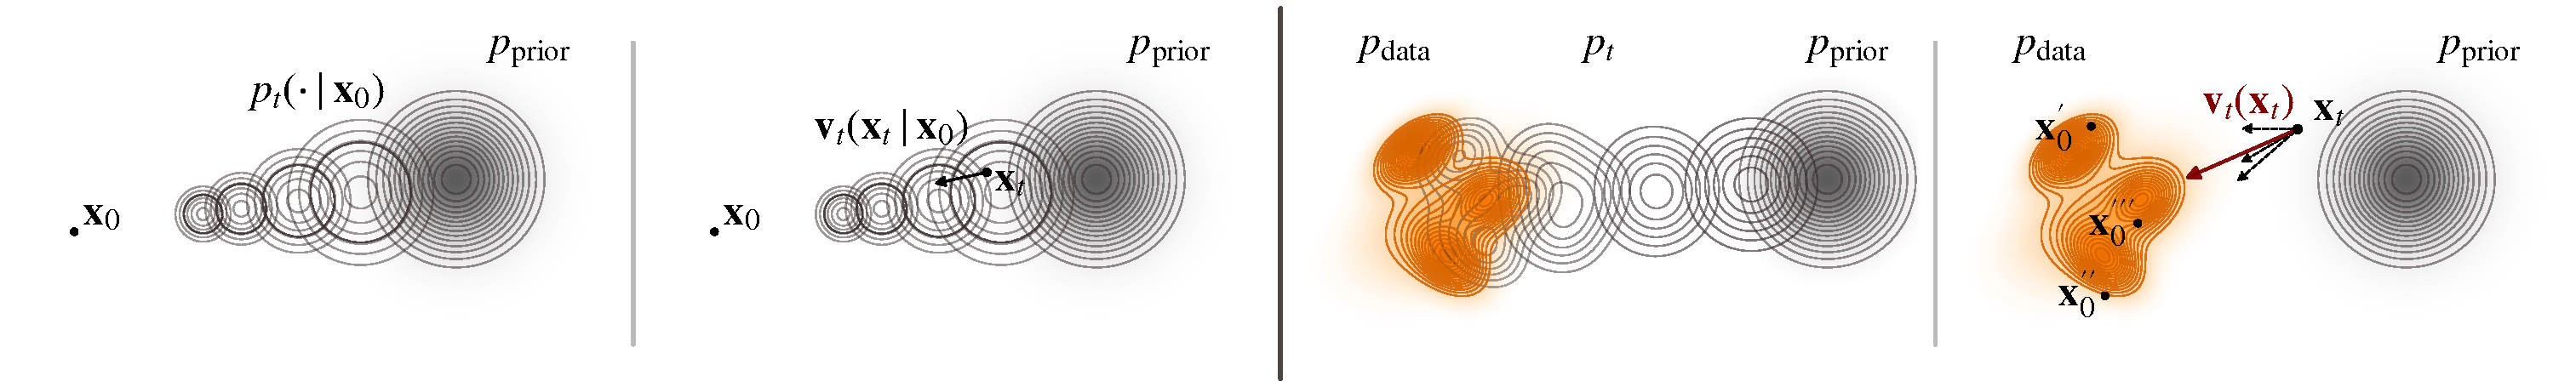
\includegraphics[width=\linewidth]{Images/PartB/four_panel_simple.pdf}
    \caption{\textbfs{扩散中条件视角与边际视角示意图。}（本图受 \citet{lipman2024flow} 启发。）
（1）条件高斯路径 $p_t(\cdot|\mathbf{x}_0)$，展示从一个固定 $\mathbf{x}_0$ 向先验不断扩张的密度。
（2）条件速度 $\mathbf{v}_t(\mathbf{x}_t|\mathbf{x}_0)=f(t)\rvx_t - \tfrac{1}{2}g^2(t) \nabla_{\rvx_t} \log p_t(\rvx_t|\rvx_0)$。
（3）边际密度 $p_t$，将数据分布 $p_{\mathrm{data}}$（橙色）传输为先验 $p_{\mathrm{prior}}$（灰色）。
（4）边际速度 $\mathbf{v}_t(\mathbf{x}_t)=f(t)\rvx_t - \tfrac{1}{2}g^2(t) \nabla_{\rvx_t} \log p_t(\rvx_t)$，由 $\mathbf{x}_t$ 到多个可能起点（虚线）的条件方向取平均得到，结果为红色箭头。在采用单侧条件 $\rvz=\rvx_0$ 的 FM 框架中，
相同的示意图也适用于 $\rvv_t(\rvx_t|\rvx_0)$ 与 $\rvv_t(\rvx_t)$，
无需将它们显式地写成
$\nabla_{\rvx_t}\log p_t(\rvx_t|\rvx_0)$ 或 $\nabla_{\rvx_t}\log p_t(\rvx_t)$ 这些分数的形式。
\figcredit{由作者绘制。}}
    \label{fig:conditional-marginal}
\end{figure}

\paragraph{底层规则：Fokker–Planck 方程。}
边际密度 $p_t$ 按 Fokker–Planck 方程演化：
\begin{mdframed}
\begin{align*}
    \frac{\partial p_t(\rvx)}{\partial t} + \nabla \cdot \Bigg( \underbrace{\left(f(t)\rvx - \frac{1}{2}g^2(t) \nabla_\rvx \log p_t(\rvx)\right)}_{\rvv_t(\rvx)}  p_t(\rvx) \Bigg) = 0.
\end{align*}
\end{mdframed}
该偏微分方程保证了 PF-ODE 给出的密度与前向 SDE 的边际分布相匹配。
为看清这一点，回顾 \Cref{eq:flow-map-def} 中所定义的 PF-ODE 的 \emph{流映射} $\bPsi_{s \to t}(\rvx_s)$，它将 $s$ 时刻的初始状态 $\rvx_s$ 直接携带至其在 $t$ 时刻的状态。
从 $t=1$ 反向运行 PF-ODE 到 $t=0$，以 $\rvx_1 \sim p_{\mathrm{prior}}$ 为初值，我们通过前推公式得到依赖时间的密度：
\begin{align}\label{eq:pushforward-ode}
    p_t^{\mathrm{rev}}(\rvx)
    = \int \delta \left(\rvx - \bPsi_{1 \to t}(\rvx_1)\right) 
      p_{\mathrm{prior}}(\rvx_1) \mathrm{d}\rvx_1.
\end{align}

Fokker–Planck 方程保证所诱导的密度路径与同一演化密度相一致：
\begin{align}\label{eq:p_t-fwd-rev}
p_t^{\mathrm{rev}} = p_t.
\end{align}
特别地，这蕴含了 $p_0^{\mathrm{rev}} = p_0 = p_{\text{data}}$，从而在 $t=0$ 时刻恢复数据分布。由于 ODE 的解映射是双向的，我们也可以类似地从
$\rvx_0 \sim p_{\text{data}}$ 出发并向前求解 ODE，从而进行平行的分析。


\subsection{流匹配框架}\label{subsec:fm-framework}

\Cref{subsec:lesson-score} 的分析表明，扩散模型之所以成功，是因为它学习到了一个在分布之间进行传输并同时满足边界条件的速度场，具体而言就是分数。\Cref{eq:lesson-dm-conditional-path} 中设计的高斯条件路径，其方差 $\sigma_t^2$ 不断增长，隐式地把一个端点锚定在高斯先验上，同时允许条件密度定义在整个空间之上，从而使得基于分数的梯度计算成为可能。

本小节中，我们介绍 FM 框架，它建立在这一见解之上
（\Cref{fig:conditional-marginal} 中的同一示意图也适用于 FM 框架）
并将其推广为学习在两个任意分布
$p_{\text{src}}$ 与 $p_{\text{tgt}}$ 之间传输样本的连续流。





\paragraph{第一步：定义条件路径及其边际密度。}
考虑 $\mathbb{R}^D$ 上的任意源分布和目标概率分布 $ p_{\mathrm{src}} $ 和 $ p_{\mathrm{tgt}} $。我们令\footnote{为了与 FM 文献中的标准记号一致，相对于前面章节我们将时间轴反向：$t=0$ 对应源分布，$t=1$ 对应目标分布。}
\begin{align}\label{eq:marginal-endpoint}
    p_0(\mathbf{x}) = p_{\mathrm{src}}(\mathbf{x}), \quad p_1(\mathbf{x}) = p_{\mathrm{tgt}}(\mathbf{x}).
\end{align}

FM 隐式地定义了一个连续的中间密度族 $\{ p_t \}_{t \in [0,1]}$，在这些端点之间进行插值。每个边际 $ p_t $ 通过一个取自已知分布 $\pi(\mathbf{z})$ 的隐变量 $\mathbf{z}$ 以及一个条件分布 $p_t(\mathbf{x}_t | \mathbf{z})$ 来表示：
\begin{equation}\label{eq:p_t}
    p_t(\mathbf{x}_t) = \int p_t(\mathbf{x}_t | \mathbf{z}) \pi(\mathbf{z}) \diff \mathbf{z},
\end{equation}
其中 $(\pi(\mathbf{z}), \{p_t(\cdot|\mathbf{z})\})$ 的选取满足 \Cref{eq:marginal-endpoint} 中的边界条件。

我们注意到，一般而言边际密度 $p_t$ 是不易处理的，因为它们需要在 $\pi(\mathbf{z})$ 上积分，并且 $\pi(\mathbf{z})$ 与条件分布 $p_t(\mathbf{x}_t|\mathbf{z})$ 都可能很复杂。
尽管如此，对隐变量 $\mathbf{z}$ 加以条件化，赋予了 FM 灵活性去建模一大类超越 \Cref{subsec:lesson-score} 讨论范围的插值路径。$\mathbf{z}$ 的常见选择包括：
\begin{itemize}
    \item \textbfs{双侧条件：} $\mathbf{z} = (\mathbf{x}_0, \mathbf{x}_1) \sim p_{\text{src}}(\mathbf{x}_0) p_{\text{tgt}}(\mathbf{x}_1)$，其中 $\pi$ 将源分布和目标分布耦合在一起。这使得 FM 能够定义任意分布之间的传输。
    \item \textbfs{单侧条件：} $\mathbf{z} = \mathbf{x}_0$ 或 $\mathbf{z} = \mathbf{x}_1$。当源分布选为高斯时，这一情形尤其恢复了类似扩散的设定。
\end{itemize}

在所有情形中，条件分布 $ p_t(\mathbf{x}_t|\mathbf{z}) $ 都应具有易处理的闭式表达。我们在全文中沿用此假设，并在 \Cref{subsec:fm-instantiations} 中给出具体构造，同时在 \Cref{fig:conditional-path} 中给出示意图。


\paragraph{第二步：速度场。}
在标准扩散模型或高斯 FM 中，中间密度族 $\{p_t\}_{t \in [0,1]}$ 在构造时将其中一个端点设为标准高斯。在这一设定下，速度场 $\mathbf{v}_t$ 被唯一确定，并具有与分数相关的闭式表达（见 \Cref{eq:dm-velocity}）。

相比之下，一般的 FM 在一般的源分布和目标分布 $p_{\text{src}}$ 与 $p_{\text{tgt}}$ 之间进行插值，此时速度场不再被唯一确定（后文将解释）。

目标是寻找一个速度场 $\mathbf{v}_t(\mathbf{x})$，使得由此诱导的、能够实现逐样本变换的 ODE
\[
\frac{\diff \mathbf{x}(t)}{\diff t} = \mathbf{v}_t(\mathbf{x}(t)), \quad t \in [0,1],
\]
在每个时刻 $t$，无论从 $\mathbf{x}(0) \sim p_{\text{src}}$ 向前积分还是从 $\mathbf{x}(1) \sim p_{\text{tgt}}$ 向后积分，所产生的 $\mathbf{x}(t)$ 的边际分布都与 $ p_t$ 匹配（更形式化的讨论见 \Cref{subsec:fm-theory}）。

这一要求由 \emph{连续性方程}\footnote{即 Fokker–Planck 方程的确定性类比，不含扩散项。}刻画：
\begin{mdframed}
\begin{equation}\label{eq:continuity_eq}
    \frac{\partial p_t(\mathbf{x})}{\partial t} + \nabla \cdot \big( \mathbf{v}_t(\mathbf{x}) p_t(\mathbf{x}) \big) = 0.
\end{equation}
\end{mdframed}

任何满足 \Cref{eq:continuity_eq} 的速度场 $\mathbf{v}_t$，
都保证 ODE 流以精确地遵循
预定义 $p_t$ 的方式传输样本（详见 \Cref{subsec:fm-theory}）。
因此，求解该 ODE 即可实现从 $p_{\text{src}}$ 到
$p_{\text{tgt}}$ 的传输，同时匹配所有中间分布。

直观上，许多不同的流都可以诱导相同的边际演化。
这是因为 \Cref{eq:continuity_eq} 是一个标量方程，而
$\mathbf{v}_t$ 是 $\mathbb{R}^D$ 中的向量场，因此该方程有无穷多解。
例如，如果 $\mathbf{v}_t$ 解该方程，那么
\[
\mathbf{v}_t + \frac{1}{p_t} \tilde{\mathbf{v}}_t,
\]
也解该方程，其中 $\tilde{\mathbf{v}}_t$ 为任意无散向量场（即
$\nabla \cdot \tilde{\mathbf{v}}_t = 0$）。因此 FM 寻求一个特定的速度场 $\mathbf{v}_t$，
使其满足 \Cref{eq:continuity_eq}，从而实现沿路径 $\{p_t\}$ 的样本连续传输。
然而，对于任意分布，
$p_t$ 与 $\mathbf{v}_t$ 一般没有闭式表达。
作为一个具体示例，我们在 \Cref{subsec:special-fm-instantiations} 中
考虑高斯到高斯的桥，此时两者都可以显式计算。





\paragraph{第三步：通过条件策略进行学习。}
FM 训练的目标是用一个神经网络 $\rvv_{\bm{\phi}}$ 逼近神谕速度场 $\rvv_t$，通过最小化期望平方误差实现：
\[
\mathcal{L}_{\mathrm{FM}}(\bm{\phi}) = \mathbb{E}_{t, \rvx_t \sim p_t} \left[ \left\| \rvv_{\bm{\phi}}(\rvx_t, t) - \rvv_t(\rvx_t) \right\|^2 \right].
\]
我们将这种神经网络参数化称为 \emph{$\rvv$-预测}（速度预测），其目的是直接学习 ODE 的漂移项。

如同 \Cref{subsec:lesson-score} 中那样，神谕速度 $\rvv_t(\rvx)$ 一般是不可处理的。为此，我们引入隐变量 $\rvz \sim \pi(\rvz)$ 并通过构造定义一个条件速度场 $\rvv_t(\rvx |\rvz)$。这允许我们借助全期望公式将损失改写为\footnote{这遵循标准的分部积分论证，正如 \Cref{eq:score-matching} 推导中所用。类似地，\Cref{eq:minimum_velocity} 在分数匹配框架内采用相同的方法推导得到。
}：
\begin{mdframed}
    \begin{align}\label{eq:fm-cfm}
    \mathcal{L}_{\mathrm{FM}}(\bm{\phi}) 
    &= \underbrace{\mathbb{E}_{t, \rvz \sim \pi(\rvz), \rvx_t \sim {\color{orange}p_t(\cdot |\rvz)}} \left[ \left\| \rvv_{\bm{\phi}}(\rvx_t, t) - {\color{orange}\rvv_t(\rvx_t |\rvz)} \right\|^2 \right]}_{\mathcal{L}_{\mathrm{CFM}}(\bm{\phi})} + C,
\end{align}
\end{mdframed}
其中 $C$ 是与 $\bm{\phi}$ 无关的常数。主项 $\mathcal{L}_{\mathrm{CFM}}$ 被称为 \emph{条件流匹配}。

也就是说，最小化 $\mathcal{L}_{\mathrm{FM}}(\bm{\phi})$ 等价于最小化 $\mathcal{L}_{\mathrm{CFM}}(\bm{\phi})$，而后者提供了更易处理的形式。
要让 $\mathcal{L}_{\mathrm{CFM}}(\bm{\phi})$ 实现易处理的、免仿真训练，必须满足两个要求：
\begin{itemize}
    \item[(i)] 从条件概率路径 $p_t(\rvx_t| \rvz)$ 中采样应当简单直接（免仿真）。
    \item[(ii)] 用作回归目标的条件速度 $\rvv_t(\rvx_t| \rvz)$ 必须具有简单的闭式表达。
\end{itemize}
我们将在 \Cref{subsec:fm-instantiations} 中给出满足这些条件的显式构造。这种条件视角使得训练变得可行：模型学习的不是难以处理的无条件速度场 $\rvv_t(\cdot)$，而是易处理的条件速度场 $\rvv_t(\cdot| \rvz)$：这与去噪分数匹配直接类似。


尽管存在无穷多个与给定 $p_t$ 相容的无条件速度场，但其中一个可以通过对条件速度场取边际得到：
\begin{align}\label{eq:marginal-oracle-velocity}
\rvv_t(\rvx_t) &:= \mathbb{E}_{\rvz \sim p(\cdot|\rvx_t)} \left[ \rvv_t(\rvx_t|\rvz)\right],
\end{align}
其中期望是在 $p(\rvz|\rvx_t)$ 上取的。
我们可以证明 \Cref{eq:fm-cfm} 中条件流匹配目标的最小化子 $\rvv^*$ 恢复了这一边际速度：
\begin{align}\label{eq:minimum_velocity}
    \rvv^*(\rvx_t, t) = \rvv_t(\rvx_t).
\end{align}
因此，学习匹配条件速度场 $\rvv_t(\cdot|\rvz)$ 即足以恢复一个有效的无条件速度场。

\begin{figure}[th!]
    \centering
    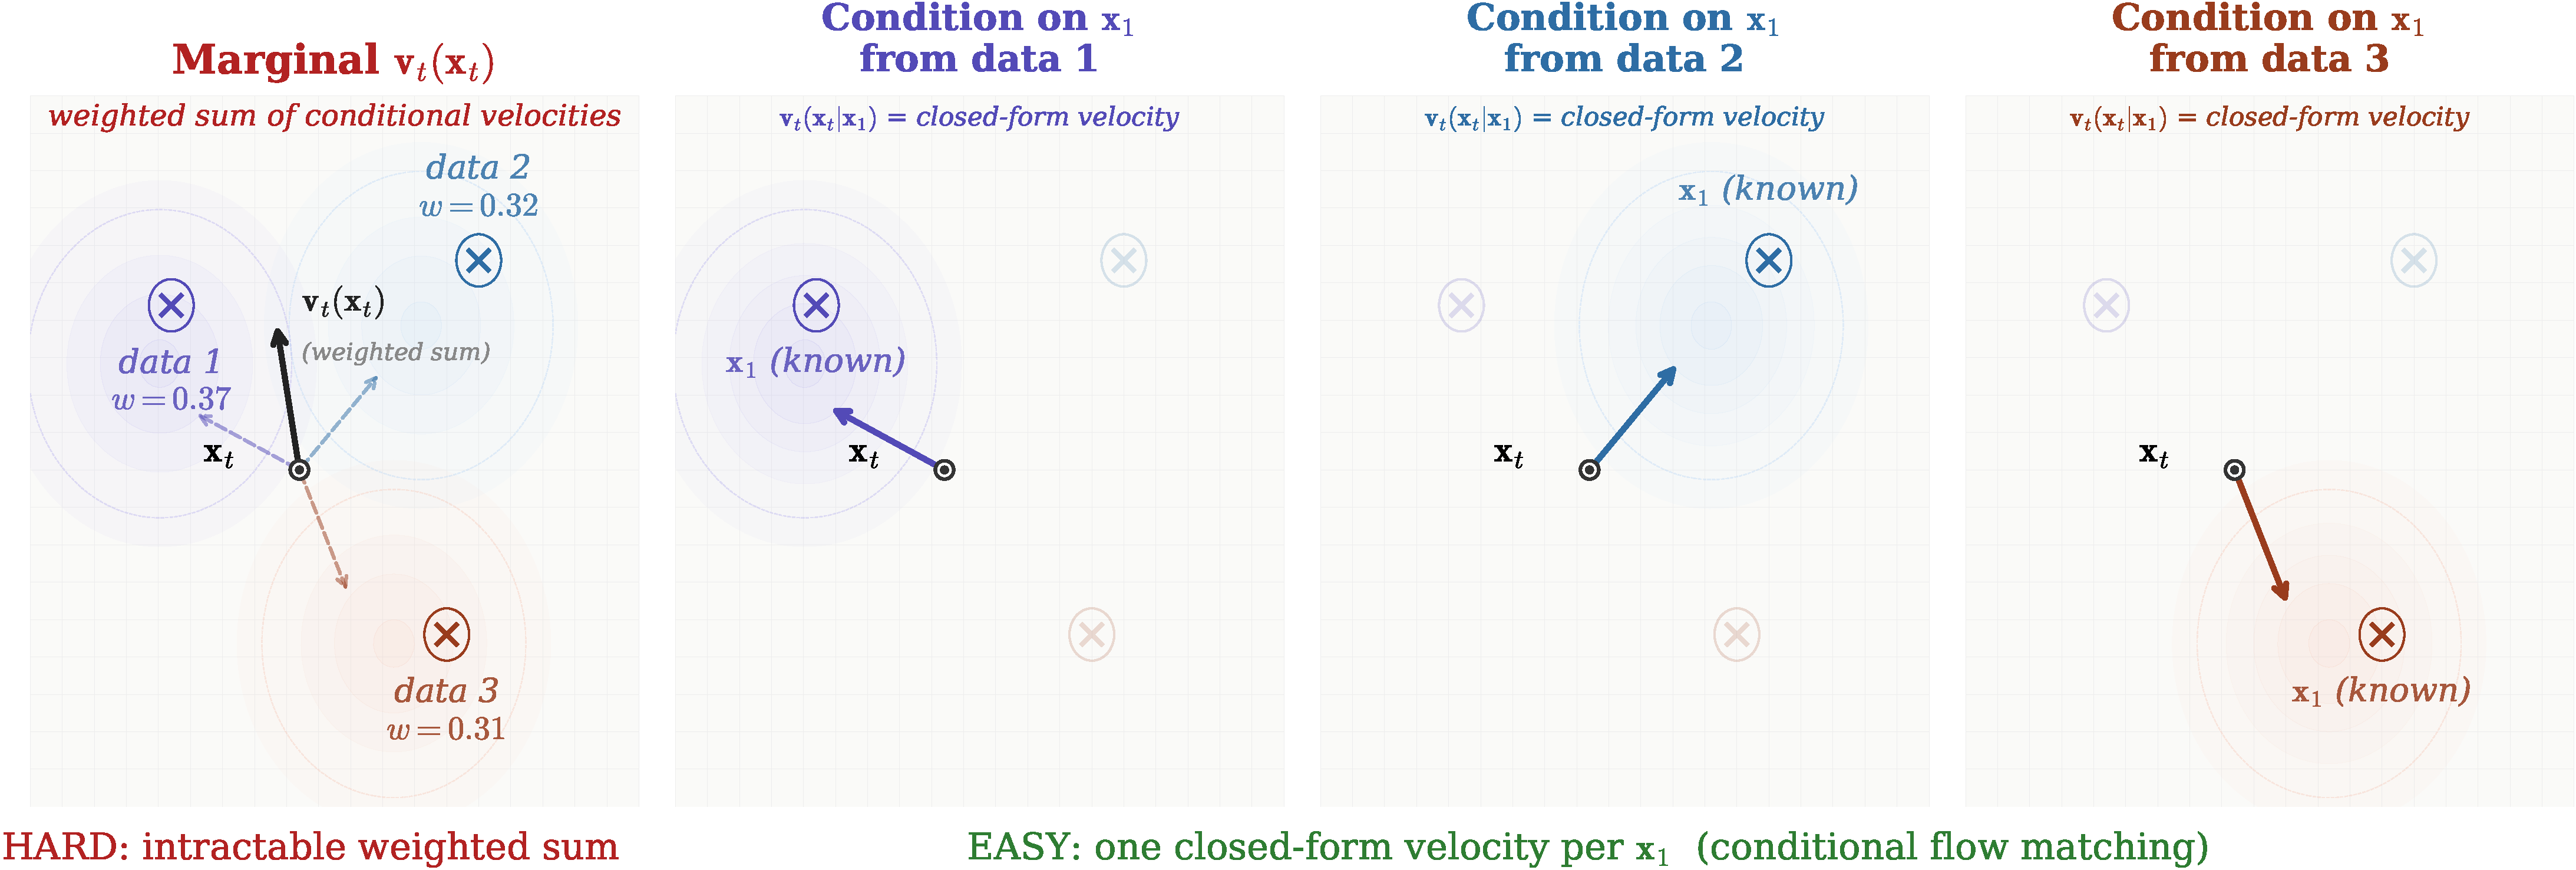
\includegraphics[width=\linewidth]{Images/PartB/flow_matching_conditional.pdf}
    \caption{\textbfs{条件流匹配中的条件技巧（取 $\rvz=\rvx_1\sim p_{\mathrm{tgt}}$）。}
边际速度
$\rvv_t(\rvx_t)=\mathbb{E}_{\rvx_1\sim p(\cdot|\rvx_t)}[\rvv_t(\rvx_t|\rvx_1)]$
（左）是所有目标点 $\rvx_1\sim p_{\mathrm{tgt}}$ 上条件速度的加权平均，权重为每个 $\rvx_1$ 产生当前 $\rvx_t$ 的似然，一般难以计算。
然而对于固定的 $\rvx_1$，条件速度具有闭式
$\rvv_t(\rvx_t|\rvx_1)=b_t'\rvx_1+(a_t'/a_t)(\rvx_t-b_t\rvx_1)$
（Proposition~\ref{closed-form-vf}；右）。
彩色箭头展示这些条件速度，黑色箭头为它们的加权平均。
条件流匹配（Theorem~\ref{thm:fm-cfm}）在这些易处理的条件目标上训练，同时达到与对难处理的边际速度进行回归相同的最优解。
这类似于变分视角中的条件技巧（Theorem~\ref{thm:equiv-marginal-kl}）以及去噪分数匹配中的条件技巧（Theorem~\ref{thm:sm-dsm}）。
\figcredit{由作者在 AI 辅助编程下绘制。}}
    \label{fig:cfm-illustration}
\end{figure}


我们将上述讨论总结如下：
\thmp{$\mathcal{L}_{\mathrm{FM}}$ 与 $\mathcal{L}_{\mathrm{CFM}}$ 的等价性}{fm-cfm}{
下式成立：
\begin{align*}
    \mathcal{L}_{\mathrm{FM}}(\bm{\phi}) = \mathcal{L}_{\mathrm{CFM}}(\bm{\phi}) + C,
\end{align*}
其中 $C$ 是与参数 $\bm{\phi}$ 无关的常数。此外，两个损失的最小化子 $\rvv^*$ 都满足
\[
    \rvv^*(\rvx_t, t) = \rvv_t(\rvx_t), \quad \text{for almost every } \rvx_t \sim p_t,
\]
其中 $\rvv_t(\rvx_t)$ 在 \Cref{eq:marginal-oracle-velocity} 中定义。
}{最小化子的论证与推导与 Proposition~\ref{dsm-minimizer} 中分数匹配情形完全相同的推理。
}

这标志着条件化技巧第三次产生了一个易处理的训练目标，如 \Cref{fig:cfm-illustration} 所示。值得注意的是，变分、基于分数以及基于流的方法都反映了相同的底层原理。



\rmkb{
取 $\pi = p_{\mathrm{data}}$，我们可以应用贝叶斯公式：
\[
p(\rvx_0|\rvx_t) = \frac{p_t(\rvx_t|\rvx_0) p_{\mathrm{data}}(\rvx_0)}{p_t(\rvx_t)},
\]
\Cref{eq:marginal-oracle-velocity} 的一个类似分解在基于分数的模型中出现：
\begin{align*}
    \nabla_{\rvx_t} \log p_t(\rvx_t) 
    &= \mathbb{E}_{\rvx_0 \sim p(\cdot|\rvx_t)} \left[ \nabla_{\rvx_t} \log p_t(\rvx_t|\rvx_0) \right] \\
    &= \mathbb{E}_{\rvx_0 \sim p_{\text{data}}} \left[ \nabla_{\rvx_t} \log p_t(\rvx_t|\rvx_0) \cdot \frac{p_t(\rvx_t|\rvx_0)}{p_t(\rvx_t)} \right],
\end{align*}
它映射了 \Cref{eq:marginal-oracle-velocity} 中的边际化策略。
}

如同 \Cref{subsec:lesson-score} 中那样，其中条件密度 $p_t(\rvx_t|\rvz)$ 和条件速度场 $\rvv_t(\rvx_t|\rvz)$ 必须被显式指定，即 $p_t(\rvx_t|\rvx_0) = \mathcal{N}(\rvx_t; \alpha_t \rvx_0, \sigma_t^2 \rmI)$ 且 $\rvv_t(\rvx_t|\rvx_0) = f(t)\rvx_t - \frac{1}{2}g^2(t)\nabla_{\rvx_t} \log p_t(\rvx_t|\rvx_0)$，一般条件流匹配框架也需要这两个组件。然而，在一般情形下我们尚未构造条件密度 $p_t(\rvx_t|\rvz)$ 或条件速度场 $\rvv_t(\rvx_t|\rvz)$。在 \Cref{sec:instance-fm} 中，我们介绍这些组件的若干常见实例。


\subsection{扩散模型、一般流匹配与 NODE 的比较}\label{subsec:compare-dm-general-fm}


\paragraph{扩散模型与一般流匹配的比较。}
来自 \Cref{subsec:lesson-score} 的见解引出了一个扩展的 FM 框架，它保留了相同的底层原理。为突出它们的相似性，我们在 \Cref{tab:framework_comparison} 中加以总结。


\begin{table}[th]
\caption{扩散模型（或高斯 FM）与一般 FM 框架之间的比较。
此处的一般 FM 框架指的是双侧条件的设定，
其中 $\mathbf{x}_0 \sim p_{\text{src}}$ 与 $\mathbf{x}_1 \sim p_{\text{tgt}}$
独立采样。}
\label{tab:framework_comparison}
\centering
\resizebox{\textwidth}{!}{
\begin{tabular}{lcc}
\toprule
\textbfs{方面} & \textbfs{（基于分数的）扩散模型} & \textbfs{一般 FM} \\
\midrule
源分布 $p_{\mathrm{src}}$ & 高斯先验 & 任意 \\
目标分布 $p_{\mathrm{tgt}}$ & 数据分布 & 任意 \\
隐变量分布 $\pi(\rvz)$ & $p_{\text{data}}$ & 见 \Cref{subsec:fm-instantiations} \\
条件分布 $p_t(\rvx_t|\rvz)$ & $\mathcal{N}(\rvx_t;\alpha_t\rvx_0,\sigma_t^2\rmI)$ & 见 \Cref{subsec:fm-instantiations} \\
边际分布 $p_t(\rvx_t)$ & $\int p_t(\rvx_t|\rvx_0) p_{\mathrm{data}}(\rvx_0) \diff\rvx_0$ & $ \int p_t(\rvx_t|\rvz) \pi(\rvz) \diff\rvz$ \\
条件速度 $\rvv_t(\rvx|\rvz)$  & $f(t) \rvx - \frac{1}{2} g^2(t) \nabla \log p_t(\rvx|\rvx_0)$ & 见 \Cref{subsec:fm-instantiations} \\
边际速度 $\rvv_t(\rvx)$  & $f(t) \rvx - \frac{1}{2} g^2(t) \nabla \log p_t(\rvx)$ & 见 \Cref{eq:marginal-oracle-velocity} \\
学习目标 & $\mathcal{L}_{\text{SM}}=\mathcal{L}_{\text{DSM}}+C$ & $\mathcal{L}_{\mathrm{FM}}=\mathcal{L}_{\mathrm{CFM}}+C$ \\
底层规则 & \multicolumn{2}{c}{Fokker-Planck / 连续性方程} \\
\bottomrule
\end{tabular}
}
\end{table}
我们指出，由于高斯 FM 本质上等价于标准扩散模型（详见 \Cref{ch:all-equivalent}），除非明确说明，否则我们将不对二者加以区分。


\paragraph{与 NODE 的联系。}
FM 可被视为 \Cref{subsec:NODE} 中介绍的 NODE 的一种免仿真替代方案。CNF 在最大似然训练时需要求解 ODE，计算开销巨大，而 FM 通过一个简单的回归损失直接回归到一个预定义的速度场，从而绕过了这一点。关键见解是，当连接源分布与目标分布的边际密度路径固定时，训练期间的精确仿真就变得不必要了。


\subsection{（可选）底层规则}\label{subsec:fm-theory}

\paragraph{连续性方程：质量守恒判据。}
类似于 \Cref{subsec:lesson-score} 中关于 PF-ODE 和 Fokker–Planck 的分析，我们现在给出一个判据，用于验证由 ODE 流诱导的密度路径是否与预定义的路径 $\{p_t\}_{t \in [0,1]}$ 相一致。

考虑在依赖时间的速度场 $\rvv_t$ 下描述粒子流的 ODE：
\[
\frac{\diff \rvx(t)}{\diff t} = \rvv_t\left(\rvx(t)\right).
\]
如同 \Cref{eq:pushforward-ode} 中那样，该 ODE 对任意 $s,t \in [0,1]$ 定义了一个流映射
$\bm{\Psi}_{s\to t}(\rvx_0)$，特别地它将 $0$ 时刻的初始点
$\rvx_0 \sim p_{\mathrm{src}}$ 携带至其在 $t$ 时刻的状态。
$t$ 时刻诱导的分布由前推给出：
\begin{align}\label{eq:ode-pushforward}
    p_t^{\mathrm{fwd}}(\rvx)
    = \int \delta \left(\rvx - \bm{\Psi}_{0\to t}(\rvx_0)\right)
      p_{\mathrm{src}}(\rvx_0) \mathrm{d}\rvx_0=: \bm{\Psi}_{0\to t}\# p_{\mathrm{src}},
\end{align}
因此当 $\rvx_0 \sim p_{\mathrm{src}}$ 时，有 $\bm{\Psi}_{0\to t}(\rvx_0) \sim p_t^{\mathrm{fwd}}$。
类似地，可以借助 $\bm{\Psi}_{1\to 0}(\rvx_1)$ 从 $\rvx_1 \sim p_{\mathrm{tgt}}$
反向传输到 $p_{\mathrm{src}}$。




假设我们给定了一条预定义的密度路径 $\{p_t\}_{t \in [0,1]}$，并构造一个速度场 $\{\rvv_t\}_{t \in [0,1]}$ 来定义粒子流。这自然引出了一个问题：

\begin{question}
    在什么条件下，流诱导的密度 $p_t^{\mathrm{fwd}}$ 在所有 $t \in [0,1]$ 上恰好匹配目标密度 $p_t$？
\end{question}
一旦这两个密度演化相一致，我们就可以通过求解 ODE 利用 ODE 流在 $p_{\mathrm{src}}$ 和 $p_{\mathrm{tgt}}$ 之间灵活地传输样本。

如同 \Cref{eq:p_t-fwd-rev} 中那样，验证这种一致性的一个有原则的方法是借助 \emph{连续性方程}，它刻画了时间演化密度中的质量守恒：

\thmp{质量守恒判据}{continuity-mass}{
流诱导的密度 $p_t^{\mathrm{fwd}}$ 在所有 $t \in [0,1]$ 上等于预定义路径 $p_t$；即
\[
p_t^{\mathrm{fwd}} = p_t, \quad \text{for all } t \in [0,1],
\]
当且仅当对 $(p_t, \rvv_t)$ 满足连续性方程：
\[
\partial_t p_t(\rvx) + \nabla_\rvx \cdot (p_t(\rvx) \rvv_t(\rvx)) = 0,
\]
对所有 $t\in[0,1]$ 和 $\rvx$ 成立。
}{\Cref{app-sec:mass-conservation} 中给出了概念性推导，更严格的处理可参见 \citep{villani2008optimal}（参见其中的“Mass Conservation Formula”）。}

\paragraph{从条件路径到边际路径。}正如 \Cref{subsec:fm-framework} 所见，我们先定义一个条件概率路径 $p_t(\cdot| \rvz)$ 和相应的条件速度场 $\rvv_t(\cdot| \rvz)$。然后我们通过下式构造边际速度场：
\[
    \rvv_t(\rvx) 
    = \int \rvv_t(\rvx| \rvz) \frac{p_t(\rvx| \rvz) \pi(\rvz)}{p_t(\rvx)}   \diff \rvz,
\]
如 \Cref{eq:marginal-oracle-velocity} 所述。然而，我们仍需确保所得边际速度 $\rvv_t$ 诱导的 ODE 流的密度路径与预定义的 $p_t$ 相一致。幸运的是，这一验证可以完全在条件层面进行：如果每个条件速度场 $\rvv_t(\cdot| \rvz)$ 诱导的条件密度路径为 $p_t(\cdot| \rvz)$，那么所得的边际速度 $\rvv_t$ 也会诱导正确的边际路径。形式化地，这表述如下：

\proppp{边际速度场生成给定边际密度}{marginal-vf}{
若条件速度场 $\rvv_t(\cdot|\rvz)$ 诱导的条件密度路径与 $p_t(\cdot|\rvz)$ 相匹配（从 $p_0(\cdot|\rvz)$ 出发），则 \Cref{eq:marginal-oracle-velocity} 中定义的边际速度场 $\rvv_t(\cdot)$ 诱导的边际密度路径与 $p_t(\cdot)$ 相一致，从 $p_0(\cdot)$ 出发。
}{
该结果通过验证对 $(p_t, \rvv_t)$ 满足连续性方程得到。我们以反过来的方式给出论证，以提供关于为何边际化后的速度场取 \Cref{eq:marginal-oracle-velocity} 这一形式的直观理解。
由于条件速度场 $\rvv_t(\cdot|\rvz)$ 对 $\rvz \sim \pi$ 诱导的密度路径与条件密度 $p_t(\cdot|\rvz)$ 相匹配，连续性方程对每个条件对成立：
\begin{align}\label{eq:continuity_conditional_pt}
    \frac{\diff}{\diff t} p_t(\rvx|\rvz) =- \nabla_\rvx \cdot \big(\rvv_t(\rvx|\rvz) p_t(\rvx|\rvz)\big).
\end{align}
我们希望找到一个速度场 ${\color{orange}\rvv_t(\cdot)}$，其诱导的密度与边际密度 $p_t$ 相一致，即满足
\begin{align}\label{eq:p_t_continuity}
    \frac{\diff}{\diff t} p_t(\rvx) =- \nabla_\rvx \cdot \big({\color{orange}\rvv_t(\rvx)} p_t(\rvx)\big).
\end{align}
从 \Cref{eq:p_t} 中 $p_t$ 的定义出发，
\begin{align*}
  \frac{\diff}{\diff t} p_t(\rvx) &=\int \frac{\diff}{\diff t} p_t(\rvx_t|\rvz)\pi(\rvz)\diff \rvz \nonumber\\
  &=  - \int \nabla_\rvx \cdot\Big(  \rvv_t(\rvx|\rvz) p_t(\rvx | \rvz)  \Big)\pi(\rvz) \diff \rvz \quad \nonumber \\
  &=  -\nabla_\rvx \cdot \Big( \int  \rvv_t(\rvx|\rvz) p_t(\rvx | \rvz) 
 \pi(\rvz) \diff \rvz\Big), \nonumber  
\end{align*}
其中第二个等号由应用 \Cref{eq:continuity_conditional_pt} 得到。将其与 \Cref{eq:p_t_continuity} 的右边相比较可知，至多差一个无散项，
\[
    {\color{orange}\rvv_t(\rvx)} p_t(\rvx) = \int \rvv_t(\rvx|\rvz) p_t(\rvx|\rvz) \pi(\rvz) \diff \rvz.
\]
因此我们可以定义
\[
    {\color{orange}\rvv_t(\rvx)} := \int \rvv_t(\rvx|\rvz) \frac{p_t(\rvx|\rvz)}{p_t(\rvx)} \pi(\rvz) \diff \rvz,
\]
这正是 \Cref{eq:marginal-oracle-velocity} 中的形式。
本定理的证明本质上沿着与此论证相反的方向进行。
}

这一联系使我们可以将构造潜在的不可处理的边际速度场，归约为定义更简单的条件速度场 $\rvv_t(\cdot| \rvz)$，而后者按构造更易于处理。




\newpage

\section{在分布之间构造概率路径与速度}\label{sec:instance-fm}

流匹配的本质在于将一个源分布逐步变换为目标分布。为引导这一变换，需要两个关键要素：\emph{概率路径} $p_{t}$，它在每个时刻 $t$ 提供演化分布的一个快照；以及 \emph{速度场} $\rvv_{t}$，它描述单个粒子如何沿路径移动。这两个对象并非独立；它们通过连续性方程相联系，后者保证粒子动力学与分布的演化相一致。因此，学习任务归结为寻找一个忠实驱动该过程的速度场 $\rvv_t$。然而困难在于，对于一般且复杂的分布，真实的边际速度 $\rvv_t$ 是未知的，留下一个无法直接访问的不可处理目标。

条件流匹配的核心思想是通过构造一个人为但易处理的过程，来应对真实边际速度的不可处理性。为此，我们引入一个条件变量 $\rvz$，并设计一个条件速度 $\rvv_t(\rvx_t|\rvz)$ 和/或一个条件路径 $p_t(\rvx_t|\rvz)$，它们被刻意选得简单。

 因为这些条件对象具有已知的闭式形式，它们可作为模型回归的替代目标。只要满足两个实际要求，这就导出了一个有效的训练损失 $\mathcal{L}_{\mathrm{CFM}}$：（i）我们能从 $p_t(\cdot|\rvz)$ 中高效采样；（ii）相应的速度 $\rvv_t(\cdot|\rvz)$ 具有闭式表达。


我们应当如何设计一个良好行为的条件过程？为获得启发，我们转向那个已被完全理解的情况：高斯到高斯的桥（\Cref{subsec:special-fm-instantiations}）。该示例突出了两种自然的设计策略：在每个时刻 $t$ 采用高斯概率路径，或指定一个仿射速度场，两者在解析上都是易处理的。

在此见解指引下，我们以两种互补的视角将其推广到一般端点分布（另见 \Cref{subsec:cov-continuity-eq}），用于构造条件路径和速度：
\begin{itemize}
    \item \textbfs{条件概率路径优先（欧拉视角）。}先从一个条件概率路径 $p_t(\cdot|\rvz)$ 出发，再推导相应的条件速度场。
    \item \textbfs{条件流优先（拉格朗日视角）。}先从一个条件流 $\bPsi_{0\to t}(\cdot|\rvz)$（通常是仿射的）出发，通过对沿轨迹关于时间求导来推导条件速度场。
\end{itemize}


在 \Cref{subsec:fm-instantiations} 中，我们详细阐述第一种方法，它表明其与 \Cref{subsec:lesson-score} 中讨论的扩散模型构造有紧密类比；而在 \Cref{subsec:prob-path-flow} 中我们给出第二种方法。这两种视角共同提供了一个定义 $p_t(\rvx_t| \rvz)$ 与 $\rvv_t(\rvx_t| \rvz)$ 的实用框架，能够实现免仿真训练以及在任意源分布和目标分布之间构造流。





\subsection{关键特例：高斯到高斯桥中的边际 $p_t(\rvx_t)$ 与速度 $\rvv_t(\rvx_t)$}\label{subsec:special-fm-instantiations}

我们从高斯端点的情形开始，此时我们可以解析地计算边际密度 $p_t(\rvx_t)$ 和速度场 $\rvv_t(\rvx_t)$。这为一般情形下条件密度 $p_t(\rvx_t |\rvz_t)$ 和速度场 $\rvv_t(\rvx_t |\rvz_t)$ 的构造提供了一个模板。



当源分布和目标分布 $p_{\text{src}}$ 与 $p_{\text{tgt}}$ 都为高斯时，速度场 $\rvv_t(\cdot)$ 具有闭式表达。我们考虑如下的插值边际密度路径：
\begin{align}\label{eq:gaussian-density-path}
    p_t(\rvx_t) = \mathcal{N}\left(\rvx_t; \bm{\mu}(t), \sigma^2(t) \rmI\right),
\end{align}
具有随时间变化的均值 $\bm{\mu}(t)$ 和方差 $\sigma^2(t)>0$。两个端点由下式给出
\[
p_{\text{src}} = p_0 =  \mathcal{N}\left(\rvx; \bm{\mu}(0), \sigma^2(0) \rmI\right), \quad
p_{\text{tgt}} = p_1 =  \mathcal{N}\left(\rvx; \bm{\mu}(1), \sigma^2(1) \rmI\right),
\]
于是路径 $\{p_t\}_{t \in [0,1]}$ 将这些分布连接起来。

对于给定路径 $\{p_t\}_{t \in [0,1]}$，确实存在许多速度场都能诱导一个 ODE 流 $\bm{\Psi}_{0\to t}(\rvx)$ 使得 $\rvx \sim p_0$ 蕴含 $\bm{\Psi}_{0\to t}(\rvx) \sim p_t$。对于这条高斯路径，一个特别简单的实现为\footnote{在 \citep{lipman2022flow} 中，作者考虑 $\bm{\Psi}_{0\to t}(\rvx) = \bm{\mu}(t) + \sigma(t)\rvx$，它要求对 $\bm{\mu}(t)$ 与 $\sigma(t)$ 施加约束以保证边界条件。我们采用一个等价的归一化形式，可避免此类约束。}：
\begin{align}\label{eq:gaussian-sol-map}
    \bm{\Psi}_{0\to t}(\rvx) := \bm{\mu}(t) + \sigma(t) \left( \frac{\rvx - \bm{\mu}(0)}{\sigma(0)} \right).
\end{align}

对于定义的高斯路径 $p_t$（对所有 $t$ 均为高斯），诱导 \Cref{eq:gaussian-sol-map} 中 ODE 流的速度场 $\rvv_t(\cdot)$ 被唯一地以解析形式刻画如下~\citep{lipman2022flow}：

\proppp{高斯密度路径的闭式速度场}{closed-form-vf}{
设 $p_t$ 为 \Cref{eq:gaussian-density-path} 中的高斯路径。则产生 ODE 流 \Cref{eq:gaussian-sol-map} 的速度场 $\rvv_t(\cdot)$ 对于所定义的 $\bPsi_{0\to t}$ 是唯一的，并具有如下闭式表达：
\begin{equation*}
    \rvv_t(\rvx) = \frac{\sigma'(t)}{\sigma(t)} \left( \rvx - \bm{\mu}(t) \right) + \bm{\mu}'(t).
\end{equation*}
}{考虑具有初值 $\rvy$ 的 ODE：
\[
    \frac{\diff}{\diff t} \bm{\Psi}_{0\to t}(\rvy) = \rvv_t(\bm{\Psi}_{0\to t}(\rvy)).
\]
由于 $\bm{\Psi}_{0\to t}$ 可逆（因 $\sigma(t)>0$），我们可令 $\rvx = \bm{\Psi}_{0\to t}(\rvy)$ 且 $\rvy = \bm{\Psi}_{0\to t}^{-1}(\rvx) = \bm{\Psi}_{t\to 0}(\rvx)$ 得到
\[
    \bm{\Psi}_{0\to t}'\big(\bm{\Psi}_{0\to t}^{-1}(\rvx)\big) = \rvv_t(\rvx).
\]
对 \Cref{eq:gaussian-sol-map} 关于 $t$ 求导给出
\begin{equation*}
    \bm{\Psi}_{0\to t}'(\rvx) = \bm{\mu}'(t) + \sigma'(t) \left( \frac{\rvx - \bm{\mu}(0)}{\sigma(0)} \right).
\end{equation*}
解出 $\rvy = \bm{\Psi}_{0\to t}^{-1}(\rvx)$ 得
\[
    \rvy = \bm{\mu}(0) + \sigma(0) \left( \frac{\rvx - \bm{\mu}(t)}{\sigma(t)} \right).
\]
将其代入 $\bm{\Psi}_{0\to t}'(\rvx)$ 得
\[
    \rvv_t(\rvx) = \frac{\sigma'(t)}{\sigma(t)} \left( \rvx - \bm{\mu}(t) \right) + \bm{\mu}'(t),
\]
如所断言。
}
我们注意到，对于一个固定的流映射 $\bPsi_{0\to t}$（流优先视角），速度被唯一地由下式确定：
\[
\rvv_t  =  \partial_t \bPsi_{0\to t} \circ \bPsi_{0\to t}^{-1}.
\]
在此构造下，对 $(p_t,\rvv_t)$ 自动满足连续性方程。
相比之下，对于一个给定的密度路径 $t\mapsto p_t$ 而不固定 $\bPsi_{0\to t}$（概率路径优先视角），
速度场并不是唯一的。

这一区别恰好刻画了流优先视角与概率路径优先视角之间的差异。



这一闭式刻画在对隐变量 $\rvz$ 加条件化时仍然成立。
下面我们将这一见解加以推广，构造一般边际设定下的条件高斯路径 $p_t(\cdot|\rvz)$
并推导相应的条件速度场 $\rvv_t(\cdot|\rvz)$。




\subsection{$\rvv_t(\cdot|\rvz)$ 与 $p_t(\cdot|\rvz)$ 的条件概率路径优先构造}\label{subsec:fm-instantiations}


\begin{figure}[th!]
    \centering
    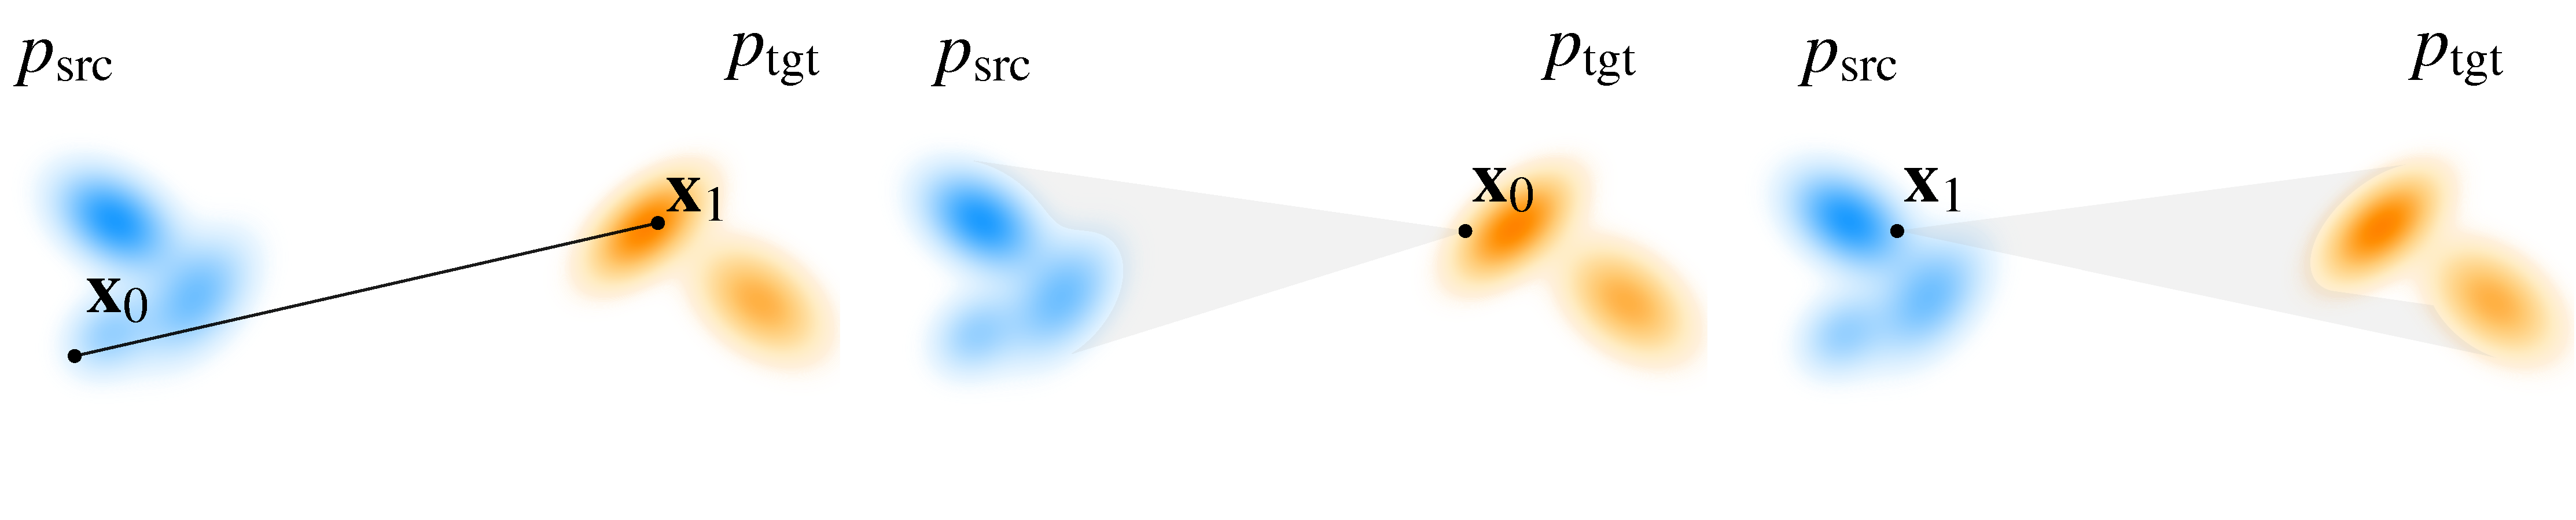
\includegraphics[width=\linewidth]{Images/PartB/triptych_gray_cones_final.pdf}
    \caption{\textbfs{两类常见条件概率路径的示意图}。包括：
（i）\emph{双侧}，以 $\rvx_0 \sim p_{\text{tgt}}$ 与 $\rvx_1 \sim p_{\text{src}}$ 为条件且端点为一般分布；
（ii）\emph{单侧}，以 $\rvx_0 \sim p_{\text{tgt}}$ 或 $\rvx_1 \sim p_{\text{src}}$ 之一为条件。
\figcredit{由作者绘制。}}
    \label{fig:conditional-path}
\end{figure}

我们的目标是先构造一个条件密度路径 $p_t(\cdot|\rvz)$，再推导其对应的条件速度场 $\rvv_t(\cdot|\rvz)$（通过 Proposition~\ref{closed-form-vf}），所基于的是关于 $\pi(\rvz)$ 的条件化。
依据 $\rvz$ 的选取方式，存在两种自然情形：
（i）双侧条件 $\rvz=(\rvx_0,\rvx_1)$，或
（ii）单侧条件 $\rvz=\rvx_0$ 或 $\rvx_1$。
在两种情形下，构造都必须匹配边界分布：
\begin{align*}
   p_{\mathrm{src}}(\rvx_0) = \int p_0(\rvx_0|\rvz) \pi(\rvz)\diff\rvz, \quad
   p_{\mathrm{tgt}}(\rvx_1) = \int p_1(\rvx_1|\rvz) \pi(\rvz) \diff\rvz.
\end{align*}
由于一旦指定了具体构造后验证这些约束非常直接，我们在此不再强调验证步骤。



\paragraph{I. 双侧 $\rvz = (\rvx_0, \rvx_1)$ —— “光束式”路径。}
    \subparagraph{$\pi(\rvz)$ 的选择。}考虑 $\mathbb{R}^D$ 上的一般分布 $p_{\mathrm{src}}$ 和 $p_{\mathrm{tgt}}$。令 $\rvz = (\rvx_0, \rvx_1)$，其中 $\rvx_0 \sim p_{\mathrm{src}}$ 与 $\rvx_1 \sim p_{\mathrm{tgt}}$ 相互独立，即
    \[
    \pi(\rvz) = p_{\mathrm{src}}(\rvx_0)  p_{\mathrm{tgt}}(\rvx_1).
    \]
    \subparagraph{条件路径 $p_t(\cdot|\rvz)$ 的选择。}用固定方差 $\sigma > 0$ 的线性插值定义条件路径：
    \[
    p_t(\rvx_t | \rvz = (\rvx_0, \rvx_1)) = \mathcal{N}(\rvx_t; a_t\rvx_0 + b_t\rvx_1,  \sigma^2 \rmI),
    \]
    其中 $a_t$ 和 $b_t$ 是依赖时间的函数，满足  $a_0 = 1,  b_0 = 0$ 和 $a_1 = 0,  b_1 = 1$。\citep{lipman2022flow,liu2022rectified} 建议的一种选取为 $a_t = 1-t$，$b_t = t$。在确定性情形 $\sigma = 0$ 下，我们得到
\[
p_t(\rvx_t |\rvz) = \delta \big(\rvx_t - [a_t\rvx_0 + b_t\rvx_1]\big),
\]
它描述了一条从 $\rvx_0$ 到 $\rvx_1$ 的确定性插值路径。
    \subparagraph{导出的条件速度 $\rvv_t(\cdot|\rvz)$。}由 Proposition~\ref{closed-form-vf}，条件速度为
    \[
    \rvv_t(\rvx | \rvz) = a'_t\rvx_0 + b'_t\rvx_1.
    \]
    \subparagraph{CFM 损失。}当 $\sigma=0$ 使得 $\rvx_t = a_t\rvx_0 + b_t\rvx_1$ 时，CFM 损失简化为
    \[
    \mathcal{L}_{\mathrm{CFM}} = \mathbb{E}_{t, \rvx_0\sim p_{\text{src}}, \rvx_1\sim p_{\text{tgt}}} \left\| \rvv_{\bm{\phi}}(\rvx_t, t) - \left(a'_t\rvx_0 + b'_t\rvx_1\right) \right\|^2.
    \]
由 \Cref{eq:marginal-oracle-velocity,eq:minimum_velocity}，最优速度场为
\[
\rvv^*(\rvx_t, t) = \mathbb{E} \left[ \rvx_t'|\rvx_t \right] = \mathbb{E} \left[ a'_t\rvx_0 + b'_t\rvx_1|\rvx_t \right].
\]
这里期望是在 $p(\mathbf{x}_0, \mathbf{x}_1|\mathbf{x}_t)$ 上取的，即在 $t$ 时刻能产生观测插值 $\mathbf{x}_t = a_t\mathbf{x}_0 + b_t\mathbf{x}_1$ 的所有源-目标对 $(\mathbf{x}_0, \mathbf{x}_1)$ 上的条件分布。



\paragraph{II. 单侧 $\rvz = \rvx_0$ 或 $\rvx_1$ —— “聚光式”路径。}
我们在单侧设定下阐述条件概率路径优先的构造，考虑标准的生成设定，即 $p_{\mathrm{src}}=\mathcal N(\bm 0,\rmI)$ 且 $p_{\mathrm{tgt}}=p_{\mathrm{data}}$。
关键的是，这一高斯源并非额外的假设，而是下面定义的条件路径的直接结果。
对任意端点更一般的处理见 \Cref{subsec:prob-path-flow}。

\subparagraph{$\pi(\rvz)$ 的选择。}
我们取 $\rvz=\rvx_1$，$\pi(\rvz)=p_{\mathrm{data}}(\rvx_1)$（$\rvz=\rvx_0\sim p_{\mathrm{prior}}$ 的情形可类似地处理）。

\subparagraph{条件路径 $p_t(\cdot|\rvz)$ 的选择。}
对固定的 $\rvx_1\sim p_{\mathrm{data}}$，定义
\[
p_t(\rvx_t|\rvz=\rvx_1)=\mathcal N \big(\rvx_t; b_t \rvx_1, a_t^2 \rmI\big),
\]
其中 $ a_0=1, b_0=0, a_1=0, b_1=1$（通常解释为极限）。
在边界处，
\[
p_0(\cdot|\rvz=\rvx_1)=\mathcal N(\cdot; \bm 0,\rmI),\qquad
p_1(\cdot|\rvz=\rvx_1)=\delta(\cdot - \rvx_1).
\]
对 $\rvx_1$ 取边际得到 $\{p_t\}_{t\in[0,1]}$，其中
$p_0=\mathcal N(\bm 0,\rmI)$（与 $p_{\mathrm{data}}$ 无关）且 $p_1=p_{\mathrm{data}}$。

\subparagraph{导出的条件速度 $\rvv_t(\cdot|\rvz)$。}
对于 $t\in(0,1)$ 且 $b_t>0$，将 Proposition~\ref{closed-form-vf} 应用于条件高斯路径得到
\[
\mathbf v_t(\rvx|\rvx_1)
= b_t' \rvx_1 + \frac{a_t'}{a_t} \big(\rvx - b_t \rvx_1\big).
\]

\subparagraph{单侧 CFM 目标。}
取 $t\sim\mathcal U(0,1)$（或任意固定的采样分布）且 $\rvx_1\sim p_{\mathrm{data}}$，CFM 损失变为
\begin{align}\label{eq:one-sided-cfm}
    \mathcal L_{\mathrm{CFM}}
=\E_{t,\rvx_1} \E_{\rvx_t\sim p_t(\cdot|\rvx_1)}
\Big\|\mathbf v_\phi(\rvx_t,t)-
\Big[b_t'\rvx_1+\tfrac{a_t'}{a_t}\big(\rvx_t-b_t\rvx_1\big)\Big]\Big\|_2^2.
\end{align}
由 MSE 最优性，唯一的最小化子是边际速度场
\[
\mathbf v^*(\rvx,t)
= \E \left[\mathbf v_t(\rvx|\rvx_1) |dle|  \rvx_t=\rvx\right]
= \E \left[a_t'\rvx_0+b_t'\rvx_1 |dle|  \rvx_t=\rvx\right].
\]

\subparagraph{与双侧目标的等价性。}
对成对样本 $(\rvx_0,\rvx_1)$ 且 $\rvx_t=a_t\rvx_0+b_t\rvx_1$，
\[
\mathbf v_t(\rvx_t|\rvx_1)
= b_t'\rvx_1 + \tfrac{a_t'}{a_t}\big(\rvx_t-b_t\rvx_1\big)
= a_t'\rvx_0 + b_t'\rvx_1.
\]
Thus the one-sided loss regresses to the \emph{conditional expectation} of the two-sided target given $\rvx_t$:
\[
\mathbf v^*(\rvx,t)=\E \big[a_t'\rvx_0 + b_t'\rvx_1 | \rvx_t=\rvx\big],
\]
so the one-sided and two-sided CFM objectives share the same minimizer.


\paragraph{Gaussian FM = Diffusion Model.}
We use the FM convention where $t=0$ denotes the source/prior and $t=1$ denotes the target/data:
\[
p_{\mathrm{src}}=p_{\mathrm{prior}},\qquad p_{\mathrm{tgt}}=p_{\mathrm{data}}.
\]
By contrast, diffusion models typically index time from data to noise (i.e., $t=0$ is data and $t=1$ is prior). 
Here, we adopt the FM convention indexing in the main discussion. For comparison, however, the VE and VP entries in \Cref{tb:interpolant_instances} are summarized in their usual diffusion-time indexing, where $t=0$ corresponds to data and $t=1$ to prior/noise.
If further $p_{\mathrm{src}}=\mathcal N(\bm 0,\rmI)$, then for fixed condition $\rvx_1\sim p_{\mathrm{data}}$, 
the conditional path $p_t(\cdot |\rvx_1)$ is naturally chosen to be Gaussian, 
while the target distribution $p_{\mathrm{tgt}}$ itself need not be Gaussian. Some literature usually refer to this setting as \emph{Gaussian FM}.



Choosing $a_t = 1-t$ and $b_t = t$ (equivalently, $\alpha_t = t$ and $\sigma_t = 1-t$ under the relabeling $a_t:=\sigma_t$, $b_t:=\alpha_t$ in diffusion model) recovers the familiar FM/RF schedule~\citep{lipman2022flow,liu2022rectified}.


\begin{table}[th]
\caption{Summary of different interpolants written as 
  $\rvx_t = a_t \rvx_0 + b_t \rvx_1$, where 
  $\rvx_0 \sim p_{\mathrm{src}}=p_{\mathrm{prior}}$ and 
  $\rvx_1 \sim p_{\mathrm{tgt}}=p_{\mathrm{data}}$. 
  The FM/RF and trigonometric columns use the FM convention ($t=0$ source, $t=1$ target). 
  For comparison, the VE/VP columns retain their usual diffusion-time indexing ($t=0$ data, $t=1$ prior/noise), with coefficient names relabeled as $a_t:=\sigma_t$ and $b_t:=\alpha_t$.}
  \small
  \centering
  \resizebox{\textwidth}{!}{
  \begin{tabular}{lcccc}
     \toprule
         & \textbfs{VE} & \textbfs{VP} & \textbfs{FM/RF} & \textbfs{Trig.}~\citep{albergo2023stochastic} \\
    \midrule
     $a_t$ (prior coeff.) 
       & $a_t$ 
       & $\sqrt{1-b_t^2}$ 
       & $1-t$ 
       & $\cos \bigl(\tfrac{\pi}{2}t\bigr)$ \\
     $b_t$ (data coeff.) 
       & $1$ 
       & $b_t$ 
       & $t$ 
       & $\sin \bigl(\tfrac{\pi}{2}t\bigr)$ \\
    \midrule
     $a_0$ & $0$ & $0$ & $1$ & $1$ \\
     $b_0$ & $1$ & $1$ & $0$ & $0$ \\
     $a_1$ & $a_1$ & $1$ & $0$ & $0$ \\
     $b_1$ & $1$ & $0$ & $1$ & $1$ \\
    \midrule
     $p_{\text{prior}}$ 
       & $\mathcal{N}(\bm{0},a_1^2\rmI)$ 
       & $\mathcal{N}(\bm{0},\rmI)$ 
       & $\mathcal{N}(\bm{0},\rmI)$ 
       & $\mathcal{N}(\bm{0},\rmI)$ \\
     \bottomrule
  \end{tabular}}
  \label{tb:interpolant_instances}
\end{table}



In the Gaussian FM setting, both the beam-like and spotlight-like conditional paths lead to training objectives that are  similar to the standard diffusion losses. As we will elaborate in \Cref{ch:all-equivalent}, Gaussian FM can in fact be equivalently interpreted as a diffusion model trained to predict the \emph{velocity}, under the linear schedule $a_t = 1-t$ and $b_t = t$. This perspective highlights that flow matching and diffusion are not fundamentally different, but rather two equivalent formulations that can be transformed into one another. The Gaussian FM objective is particularly appealing in practice: its loss function ($\E_{t,\rvx_t} \left[\norm{\rvv_\bphi(\rvx_t, t) - (\rvx_1 - \rvx_0)}_2^2\right]$) is simple, and it has been shown to achieve competitive performance at scale~\citep{esser2024scaling}. 




\subsection{Conditional Flow-First Construction of $\rvv_t(\cdot|\rvz)$ and $p_t(\cdot|\rvz)$}\label{subsec:prob-path-flow}

We treat the general case where the endpoints $p_{\mathrm{src}}$ (at $t=0$) and $p_{\mathrm{tgt}}$ (at $t=1$) are arbitrary. 
Our goal is to design, directly in trajectory space, a conditional flow that transports samples from $p_{\mathrm{src}}$ to $p_{\mathrm{tgt}}$ and yields a closed-form $\rvv_t(\rvx_t|\rvz)$ usable as a regression target.

\paragraph{Motivation.}
Instead of first designing conditional density path, we may directly specify a conditional flow map $\bPsi_{0\to t}(\cdot;\rvz)$ that moves samples along trajectories. This has two practical advantages: (i) it immediately yields a regression target for training via a time derivative along trajectories; (ii) on geometry-structured spaces (Riemannian manifolds, Lie groups, or constrained submanifolds), it is often natural to construct the conditional flow map 
$\bPsi_{0\to t}$ directly from the geometry (e.g., geodesics, exponential maps, or premetrics)~\citep{lipman2024flow} which yields analytic, simulation-free target velocities for training.


\paragraph{Conditional Affine Flow (Link to Proposition~\ref{closed-form-vf}).}
We fix a conditioning variable $\rvz\sim\pi$ (e.g., $\rvz=\rvx_1\sim p_{\mathrm{tgt}}$ in one-sided “spotlight’’ training) and push forward $\rvx_0\sim p_{\mathrm{src}}$ through the time-varying \emph{conditional affine flow} 
\[
\bPsi_{0\to t}(\rvx_0;\rvz) := \bm\mu_t(\rvz) + \rmA_t(\rvz) \rvx_0,\qquad t\in[0,1],
\]
where $\bm\mu_t(\rvz)\in\R^D$ and $\rmA_t(\rvz)\in\R^{D\times D}$ is invertible for $t\in(0,1)$. The boundary 
$\rmA_0(\rvz)=\rmI,\ \bm\mu_0(\rvz)=\mathbf 0$ recovers $p_{\mathrm{src}}$ at $t=0$. It is standard to interpret boundary when $t\to1$ as a limit (the terminal map may concentrate mass on a lower-dimensional set or a point)\footnote{Allowing $\rmA_1(\rvz)$ to be singular (e.g., $\mathbf 0$) is compatible with invertibility on $(0,1)$ and causes the path to contract onto the prescribed endpoint at $t=1$.}. 


\subparagraph{Induced Conditional Path $p_t(\cdot|\rvz)$.}
The construction defines
\[
p_t(\cdot|\rvz) = \bigl(\bPsi_{0\to t}( \cdot ;\rvz)\bigr)_{\#} p_{\mathrm{src}},
\qquad
p_t(\cdot)  =  \int p_t(\cdot|\rvz)\pi(\rvz)\diff\rvz.
\]
What ultimately matters in $\mathcal{L}_{\mathrm{CFM}}$ is how to sample from it:  
first draw $\rvz \sim \pi$, then draw $\rvx_0 \sim p_{\mathrm{src}}$, and finally set
\[
\rvx_t = \bm\mu_t(\rvz) + \rmA_t(\rvz)\rvx_0.
\]


We remark that when $\bPsi_{0\to t}$ is affine in $\rvx_0$, then $p_t( \cdot | \rvz)$ is Gaussian 
if and only if $p_{\mathrm{src}}$ is Gaussian. 
In particular, for arbitrary (non-Gaussian) $p_{\mathrm{src}}$, an affine flow yields a
generally non-Gaussian $p_t(\cdot|\rvz)$.


\subparagraph{Derived Conditional Velocity $\rvv_t(\cdot|\rvz)$.} The conditional velocity $\rvv_t(\cdot|\rvz)$ is obtained by $t$-differentiating the conditional flow map $\bPsi_{0\to t}$. Following the derivation in Proposition~\ref{closed-form-vf}, consider the \emph{conditional} ODE defined by the flow map $\bPsi_{0\to t}(\rvy;\rvz)$ with initial condition $\rvy$, where the goal is to identify the corresponding conditional velocity field $\rvv_t(\cdot|\rvz)$:
\[
\frac{\diff}{\diff t} \bPsi_{0\to t}(\rvy;\rvz)
= \rvv_t \Big(\underbrace{\bPsi_{0\to t}(\rvy;\rvz)}_{\rvx} \Big| \rvz\Big).
\]
Since $\bPsi_{0\to t}(\cdot;\rvz)$ is invertible for $t\in(0,1)$, we may express $\rvy$ in terms of the current state $\rvx:=\bPsi_{0\to t}(\rvy;\rvz)$ as $\rvy=\bPsi_{0\to t}^{-1}(\rvx;\rvz)=\bPsi_{t\to 0}(\rvx;\rvz)$. Substituting this into the ODE yields the following construction of the conditional velocity field:
\[
\rvv_t(\rvx|\rvz)
:= \frac{\diff}{\diff t} \bPsi_{0\to t} \bigl(\bPsi_{t\to 0}(\rvx;\rvz);\rvz\bigr),
\]
which makes explicit that the derivative must be taken along the trajectory that reaches the spatial point $\rvx$ at time $t$.


Since $\rvx_t=\bm\mu_t(\rvz)+\rmA_t(\rvz)\rvx_0$ and $\rmA_t(\rvz)$ is invertible on $(0,1)$, we have $\rvx_0=\rmA_t(\rvz)^{-1}\bigl(\rvx-\bm\mu_t(\rvz)\bigr)$, giving
\[
\rvv_t(\rvx|\rvz)
 = 
\bm\mu_t'(\rvz) + \rmA_t'(\rvz) \rmA_t(\rvz)^{-1} \bigl(\rvx-\bm\mu_t(\rvz)\bigr).
\]


\subparagraph{One-Sided Conditioning ($\rvz=\rvx_1$).}
Choosing $\bm\mu_t(\rvz)=b_t \rvz$ and $\rmA_t(\rvz)=a_t \rmI$ with $a_0=1,a_1=0$ and $b_0=0,b_1=1$ (with $a_t>0$ for $t\in(0,1)$) yields
\[
\rvx_t = a_t \rvx_0 + b_t \rvx_1,
\qquad
\rvv_t(\rvx|\rvx_1) = b_t' \rvx_1 + \frac{a_t'}{a_t} \bigl(\rvx-b_t\rvx_1\bigr).
\]
On paired samples $(\rvx_0,\rvx_1)$ (with $\rvx_t=a_t\rvx_0+b_t\rvx_1$), this simplifies to the usual CFM target:
\[
\rvv_t(\rvx_t|\rvx_1)=a_t' \rvx_0 + b_t' \rvx_1.
\]

\subparagraph{Two-Sided Conditioning ($\rvz=(\rvx_0,\rvx_1)$).}
The same template with $\bm\mu_t(\rvx_0,\rvx_1)=b_t \rvx_1$ and $\rmA_t(\rvx_0,\rvx_1)=a_t \rmI$ makes the conditional path \emph{deterministic}:
\[
\rvx_t=a_t \rvx_0+b_t \rvx_1,
\qquad
p_t(\cdot|\rvx_0,\rvx_1)=\delta\left(\cdot - (a_t\rvx_0+b_t\rvx_1)\right),
\]
and the conditional velocity is
\[
\rvv_t(\rvx_t|\rvx_0,\rvx_1)=a_t' \rvx_0+b_t' \rvx_1,
\]
i.e., the standard two-sided CFM target. 

\subparagraph{Unconditional Gaussian Path as a Special Case.}
If $\bm{\mu}_t$ is independent of $\rvz$ (denoted $\bm{\mu}(t)$) and 
$\rmA_t = \tfrac{\sigma(t)}{\sigma(0)} \rmI$, then
\[
\bPsi_{0\to t}(\rvx_0)=\bm\mu(t)+\sigma(t) \frac{\rvx_0-\bm\mu(0)}{\sigma(0)},
\quad
\rvv_t(\rvx)=\bm\mu'(t)+\frac{\sigma'(t)}{\sigma(t)}\bigl(\rvx-\bm\mu(t)\bigr),
\]
which recovers the Gaussian density path and the closed-form velocity in Proposition~\ref{closed-form-vf}.





\subsection{Probability-Path-First vs. Flow-First Construction}

Both constructions aim to connect a source distribution $p_{\mathrm{src}}$ and a target distribution $p_{\mathrm{tgt}}$ through conditional dynamics. 
The \emph{probability-path-first} (Eulerian) view begins by positing a conditional density path $p_t(\cdot|\rvz)$, often chosen from Gaussian or affine families so that the associated velocity $\rvv_t(\cdot|\rvz)$ can be solved analytically. 
The \emph{flow-first} (Lagrangian) view instead specifies a conditional flow map $\bPsi_{0\to t}(\cdot|\rvz)$ and obtains the velocity directly by differentiation along particle trajectories. 
While both yield equivalent transport under regularity, they differ in identifiability, ease of computation, and how endpoint constraints are enforced. 
The following table summarizes these contrasts. The takeaway: path-first is natural when conditional paths admit closed-form velocities; flow-first is natural when you have strong structural priors on trajectories.

\newpage
\begin{center} \begingroup \scriptsize \setlength{\tabcolsep}{4pt} \renewcommand{\arraystretch}{1.05} \begin{tabular}{p{0.13\linewidth} p{0.41\linewidth} p{0.41\linewidth}} \toprule \textbfs{Axis} & \textbfs{Conditional Probability-Path-First} & \textbfs{Conditional Flow-First} \\\midrule \textbfs{Given} & Conditional density path $p_t(\cdot|\rvz)$. & Conditional flow map $\bPsi_{0\to t}(\cdot|\rvz)$ (trajectories, for each fixed $\rvz$). \\ \graymidrule \textbfs{Get Velocity} & For each $\rvz$, find $\rvv_t(\cdot|\rvz)$ s.t.\ $$\partial_t p_t(\cdot|\rvz)+\nabla \cdot \left(p_t(\cdot|\rvz) \rvv_t(\cdot|\rvz)\right)=0;$$ Non-unique: if $\nabla\!\cdot~\left(p_t \mathbf w_t\right)=0$ then $\rvv_t+\mathbf w_t$ yields the same $p_t$. & Along paths (for each $\rvz$): $$ \rvv_t \left(\bPsi_{0\to t}(\cdot|\rvz) | \rvz\right)=\tfrac{\diff}{\diff t}\bPsi_{0\to t}(\cdot|\rvz).$$ 
When $\bPsi_{0\to t}$ is invertible, one can solve
$$\rvv_t(\rvx|\rvz) = \tfrac{\diff}{\diff t}\bPsi_{0\to t}(\bPsi_{0\to t}^{-1}(\rvx)|\rvz). $$
\\ \graymidrule \textbfs{Closed Form \newline of  $\rvv_t(\cdot|\rvz)$} & Convenient when $p_t(\cdot|\rvz)$ is Gaussian / exponential-family; otherwise obtaining $\rvv_t(\cdot|\rvz)$ is nontrivial. & Convenient when $\bPsi_{0\to t}(\cdot|\rvz)$ has structure (affine/low-rank); avoids density evaluation. \\ \graymidrule \textbfs{Uniqueness \newline of  $\rvv_t(\cdot|\rvz)$} & For each $\rvz$, $\rvv_t(\cdot|\rvz)$ is underdetermined unless a selection rule (e.g., potential flow / min.\ kinetic energy) is imposed. & Given $\bPsi_{0\to t}(\cdot|\rvz)$, both $p_t(\cdot|\rvz)=(\bPsi_{0\to t}(\cdot|\rvz))_\#p_0$ and $\rvv_t(\cdot|\rvz)$ are determined; non-invertible maps still define $\rvv_t(\cdot|\rvz)$ along trajectories, while invertible ones make it unique.
 \\ \graymidrule \textbfs{Realizability} & Must verify the constructed $\rvv_t(\cdot|\rvz)$ solving the continuity equation on the intended support. & Holds by construction: $$p_t(\cdot|\rvz)=\left(\bPsi_{0\to t}(\cdot|\rvz)\right)_\# p_0(\cdot|\rvz).$$ \\ \graymidrule \textbfs{Match \newline $(p_{\mathrm{src}},p_{\mathrm{tgt}})$} & Mix conditionals: \newline \hspace{3cm}$ p_{\mathrm{src}} = \int p_0(\cdot|\rvz) \pi(\rvz)\diff\rvz,$ \newline $p_{\mathrm{tgt}} = \int p_1(\cdot|\rvz) \pi(\rvz)\diff\rvz.$ \newline Under Gaussian--affine conditional paths with $\rvz$-independent coefficients, 
$p_{\mathrm{src}}$ can be forced to be Gaussian. 
For a general fixed endpoint $p_{\mathrm{src}}$ (possibly non-Gaussian), 
the choice of $p_t(\cdot|\rvz)$ does not generally pin $p_{\mathrm{src}}$.
 & Set $\bPsi_{0\to 0}=\mathrm{Id}$ and choose boundary condition  to hit any $p_{\mathrm{tgt}}$. \\ \graymidrule \textbfs{Preferred \newline Scenarios} & Diffusion-style constructions; analytic targets via conditional Gaussians $p_t(\cdot|\rvz)$. & Strong structural priors via maps $\bPsi_{0\to t}(\cdot|\rvz)$; easy boundary control; accommodates singular/low-dimensional endpoints; natural for
map-based regularization/transport
costs. \\ \bottomrule \end{tabular} \endgroup \end{center}





%%%%%%%%%%%%%%%%%
\subsection{On the Misinterpreted ``Straightness'' of the Canonical Affine Path}

It is worth emphasizing that some prior
works~\citep{liu2022rectified,lipman2022flow} suggest that adopting the
canonical affine flow, $a_t = 1-t$ and $b_t = t$, yields
``straight-line'' ODE trajectories enabling faster sampling. However,
this claim does not hold in general.

The key point is that one must distinguish two different notions of
straightness. Under the canonical affine interpolation
\[
\rvx_t = (1-t)\rvx_0 + t\rvx_1,
\]
each \emph{conditional} path is indeed a straight-line interpolation in
time once a particular pair $(\rvx_0,\rvx_1)$ is fixed. 

However, the actual sampling dynamics are governed not by a single fixed
pair $(\rvx_0,\rvx_1)$, but by the \emph{marginal} velocity field
\[
\rvv^*(\rvx,t) = \E[\rvx_1 - \rvx_0| \rvx_t = \rvx].
\]
This is a conditional average over all pairs $(\rvx_0,\rvx_1)$ that
could have produced the same intermediate point $(\rvx,t)$. As $t$
changes, this conditional distribution changes, and so the averaged
velocity generally changes as well. Consequently, the marginal ODE
trajectory
\[
\frac{\diff \rvz_t}{\diff t} = \rvv^*(\rvz_t, t) 
\]
need not be a straight-line interpolation in time, even though every
underlying conditional path is straight. Therefore, while the scheduler $(a_t,b_t)=(1-t,t)$ can still be useful
in practice, any empirical gain should not be attributed solely to a
supposed ``straightness'' of the resulting ODE trajectories. In
particular, since the marginal ODE trajectories are not generally
straight, this choice alone does not imply that one can use fewer solver
steps while still sampling the ODE accurately.

We now illustrate this point with a simple closed-form counterexample.

\exm{A Simple 1D Counterexample}{
Consider the one-dimensional setting with
\[
x_0 \sim \mathcal{N}(0, \sigma_0^2),
\qquad
x_1 \sim \mathcal{N}(0, \sigma_1^2),
\]
independent coupling, and the canonical affine interpolation
$x_t = (1-t)x_0 + tx_1$.
Each conditional path $(1-t)x_0 + tx_1$ is a straight line in
time. We now compute the induced marginal velocity field.

Since $(x_1 - x_0,\, x_t)$ is jointly Gaussian, the
conditional expectation is linear in $x$, so
\[
v^*(x,t)
= \E[x_1 - x_0| x_t = x]
= \frac{\operatorname{Cov}(x_1 - x_0,\, x_t)}
       {\operatorname{Var}(x_t)}\, x.
\]
A direct calculation gives
\[
\operatorname{Var}(x_t)
= (1-t)^2\sigma_0^2 + t^2\sigma_1^2
=: V(t),
\]
and
\[
\operatorname{Cov}(x_1 - x_0,\, x_t)
= t\sigma_1^2 - (1-t)\sigma_0^2
= \tfrac{1}{2} V'(t).
\]
Hence
\[
v^*(x,t) = \frac{V'(t)}{2V(t)}\, x.
\]

The marginal ODE
\[
\frac{\diff z_t}{\diff t} = v^*(z_t, t)
\]
therefore has the exact solution
\[
z_t
= z_0 \sqrt{\frac{V(t)}{V(0)}}
= z_0 \sqrt{(1-t)^2 + \frac{\sigma_1^2}{\sigma_0^2}\, t^2}.
\]

Now, a straight-line interpolation in time would require $z_t$ to be
affine in $t$, namely $z_t = (1-t)z_0 + t\,z_1$ for some endpoint
$z_1$. But
\[
\sqrt{(1-t)^2 + \frac{\sigma_1^2}{\sigma_0^2}\, t^2}
\]
is not affine in $t$ for any positive $\sigma_0, \sigma_1$. Thus the ODE
trajectory is generally not a straight-line interpolation in time. We illustrate this phenomenon in \Cref{fig:straightness-counterexample}
with the example $\sigma_0=2$ and $\sigma_1=3$.

For example, when $\sigma_0 = \sigma_1$, we have $z_1 = z_0$, so a
straight-line interpolation would simply be the constant path
$z_t = z_0$. In contrast, the actual ODE trajectory satisfies
\[
z_{1/2} = \frac{z_0}{\sqrt{2}} \neq z_0.
\]
Therefore, even though every conditional interpolation path is straight,
the induced marginal ODE trajectory need not be.
}
%%%%%%%%%%%%%

\begin{figure}[th]
        \label{fig:straightness-counterexample}
    \centering
    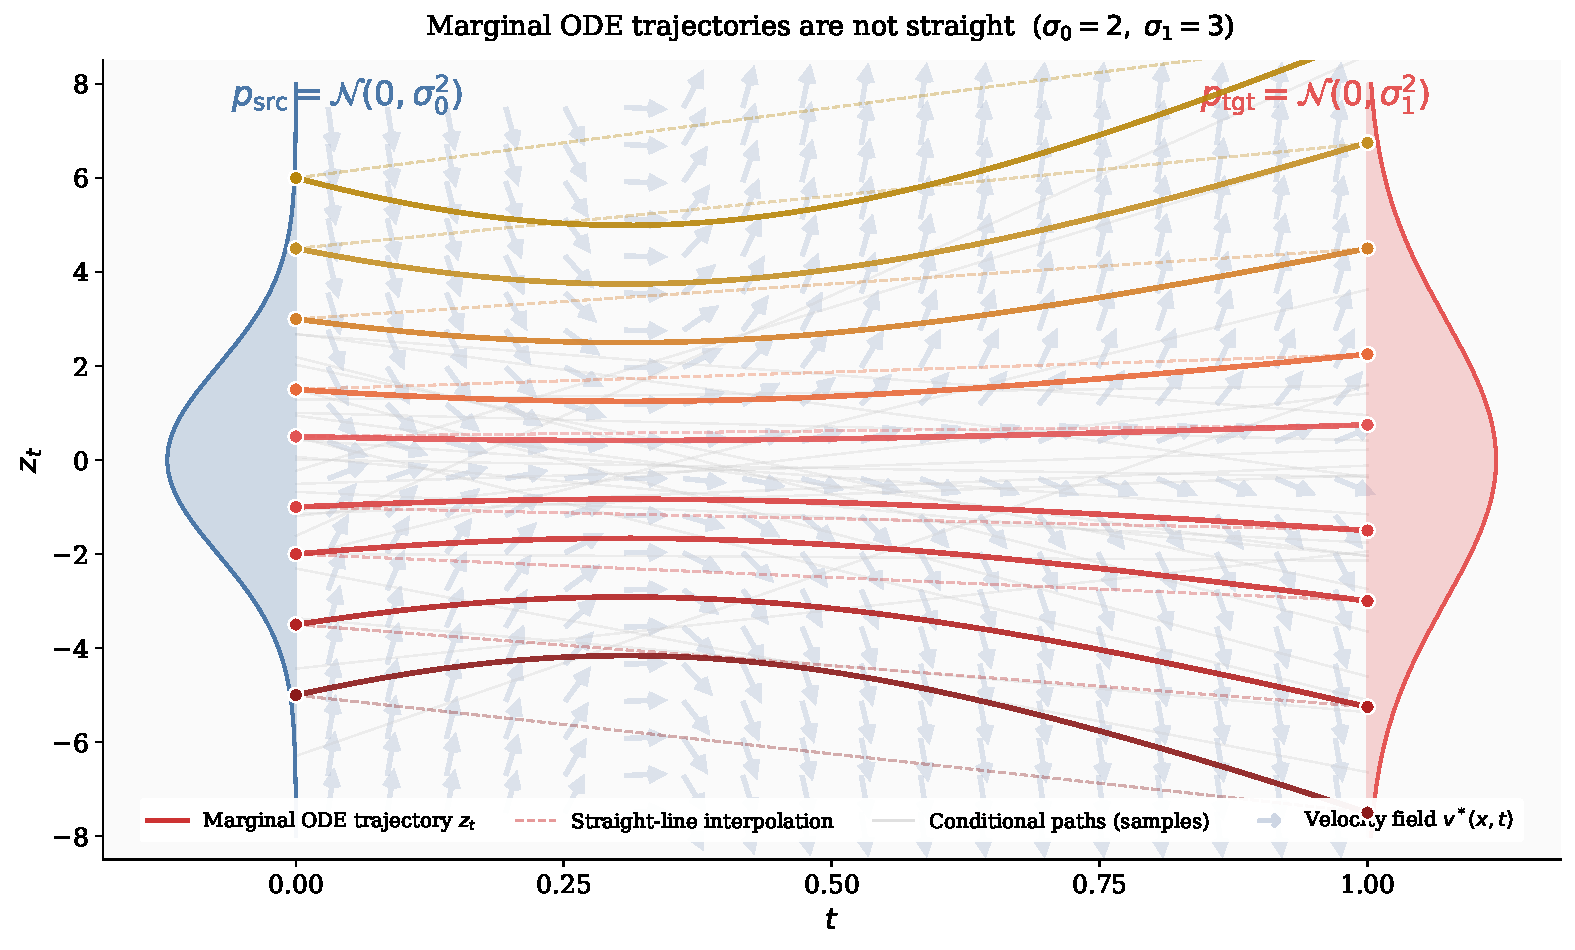
\includegraphics[width=\linewidth]{Images/PartB/straightness_counterexample.pdf}
    \caption{\textbfs{Marginal ODE trajectories are not straight under the canonical affine interpolation.}
    We take $x_0 \sim \mathcal{N}(0, \sigma_0^2)$ and $x_1 \sim \mathcal{N}(0, \sigma_1^2)$ with $\sigma_0=2$, $\sigma_1=3$, and independent coupling.
    Gray lines show sampled conditional paths $(1-t)x_0 + tx_1$, which are straight by construction.
    Solid curves show the exact marginal ODE trajectories $z_t = z_0\sqrt{(1-t)^2 + (\sigma_1/\sigma_0)^2 t^2}$, and dashed lines show the corresponding straight-line interpolations from $z_0$ to $z_1$.
    The visible gap between solid and dashed curves confirms that the marginal ODE trajectories are not affine in $t$, even though every conditional path is a straight line.
    The marginal densities $p_{\mathrm{src}}$ and $p_{\mathrm{tgt}}$ are shown on the left and right margins, respectively.
    \figcredit{Created by the authors with AI-assisted coding.}}
\end{figure}
     





%%%%%%%%%%%%%%%%%%%%%%%%%%%%%%%%%%%%%%%%%%%%%%%%%%%%%%%%%%%%%%%%%%%%%%%%
\clearpage
\newpage
%%%%%%%%%%%%%%%%%%%%%%%%%%%%%%%%%%%%%%%%%%%%%%%%%%%%%%%%%%%%%%%%%%%%%%%%

S\section{\texorpdfstring{(Optional) Properties of the Canonical Affine Flow}{(Optional) Properties of the Canonical Affine Flow}}\label{sec:optimal-canonical}

Given two endpoint distributions $p_0=p_{\mathrm{src}}$ and $p_1=p_{\mathrm{tgt}}$, 
a natural and widely used choice for defining the conditional path in flow matching (FM)~\citep{lipman2022flow} 
and rectified flow (RF)~\citep{liu2022flow} is the linear interpolation
\[
a_t = 1 - t, \qquad b_t = t,
\]
which yields the interpolant
\[
\mathbf{x}_t = (1 - t)\mathbf{x}_0 + t \mathbf{x}_1, 
\qquad \mathbf{x}_0 \sim p_{\mathrm{src}},\ \mathbf{x}_1 \sim p_{\mathrm{tgt}}.
\]
Under this choice, the training objective simplifies to
\[
\mathbb{E}_{t \sim \mathcal{U}[0,1]}   
\mathbb{E}_{\mathbf{x}_0, \mathbf{x}_1} 
\left[ \bigl\|\mathbf{v}_{\bm{\phi}}(\mathbf{x}_t, t) - (\mathbf{x}_1 - \mathbf{x}_0)\bigr\|_2^2 \right].
\]

This linear flow enjoys several appealing properties. 
In particular, it admits an iterative refinement scheme, known as \emph{\texttt{Reflow}}, 
which progressively straightens the path between distributions while preserving the marginals. 





\subsection{Rectifying Flows: From Noisy Guesses to Structured Pairings}\label{subsec:rectify}

\paragraph{From Noise to Data via Coherent Paths.}
Take the generation task where $p_{\text{src}}$ is the prior and $p_{\text{tgt}}$ is the real data. We want a continuous path that transports noise to data. A naive tactic samples $\rvz_0 \sim p_{\text{src}}$ and $\rvx_1 \sim p_{\text{tgt}}$ independently, interpolates (e.g.\ $\rvx_t=(1-t)\rvx_0+t\rvx_1$), and fits a velocity field to that line. This creates \emph{incoherent pairings}: endpoints are unrelated across iterations, so trajectories fluctuate, variance explodes, convergence slows, and sample quality suffers.

\paragraph{Why Independent Couplings Fall Short.}
Conditional flow matching with independent draws uses
\[
\pi(\rvz)=p_{\text{src}}(\rvx_0) p_{\text{tgt}}(\rvx_1),
\]
or one-sided variants. Such couplings are sampling-friendly but induce jagged, high-variance paths that a velocity field struggles to model.

\paragraph{Rectify the Flow via Dependent Coupling.}
Rather than relying on arbitrary pairings, we use a pre-trained diffusion model $\rvv_{\bphi^\times}(\cdot,t)$ as the drift in a PF-ODE to \emph{deterministically} transport each source point. Starting from $\rvz(0)=\rvz_0 \sim p_{\text{src}}$, we integrate
\[
\frac{\diff \rvz(t)}{\diff t} = \rvv_{\bphi^\times}(\rvz(t),t), \qquad t \in [0,1],
\]
to obtain $\hat\rvz_1 := \rvz(1)$ positioned near the data space learned from the pre-trained model. The resulting pair $(\rvz_0,\hat\rvz_1)$ forms a \emph{dependent coupling}: it follows a structured, model-guided path rather than an arbitrary interpolation. This idea extends naturally to affine reference paths of the form $\rvx_t = a_t \rvx_0 + b_t \rvx_1$, where $\rvx_0 \sim p_{\text{src}}$ and $\rvx_1 \sim p_{\text{tgt}}$.



\begin{algorithm}[H]
\caption{\texttt{Rectify} Operation\label{alg:Rectify}}
\begin{algorithmic}[1]
\Require Reference path $\{\rvx_t\}_{t\in[0,1]}$ (e.g.\ $\rvx_t=a_t\rvx_0+b_t\rvx_1$)
\State \textbfs{Pre-Train Diffusion.} Fit $\rvv_{\bphi^\times}$ on the chosen path by minimizing
\[
\bphi^\times \in \arg\min_{\bphi} 
\mathbb{E}_{t,\rvx_0,\rvx_1} \left[\Big\|\rvv_{\bphi}(\rvx_t,t)-\frac{\diff \rvx_t}{\diff t}\Big\|_2^2\right].
\]
\State \textbfs{Rectify.} Sample $\rvz_0 \sim p_{\text{src}}$ and integrate
\[
\frac{\diff \rvz(t)}{\diff t}=\rvv_{\bphi^\times}(\rvz(t),t),\qquad \rvz(0)=\rvz_0,\quad t\in[0,1],
\]
to obtain $\hat\rvz_1=\rvz(1)$ and the trajectory $\{\rvz(t)\}_{t\in[0,1]}$.
\Ensure Dependent (coherent) pair $(\rvz_0,\hat\rvz_1)$ or the full trajectory.
\end{algorithmic}
\end{algorithm}

\paragraph{Why It Works: Marginal-Preserving Structure.}
Let $\bPhi_{0\to t}$ denote the flow map generated by the above ODE defined by the pre-trained diffusion $\rvv_{\bphi^\times}$; then $\rvz(t)=\bPhi_{0\to t}(\rvz_0)$ and $\hat\rvz_1=\bPhi_{0\to 1}(\rvz_0)$. The \texttt{Rectify} procedure pairs each source point with its flow endpoint, giving the deterministic joint
\[
\pi_{\text{Rectify}}(\rvz_0,\rvz_1)
= p_{\text{src}}(\rvz_0) \delta \big(\rvz_1-\bPhi_{0\to 1}(\rvz_0)\big).
\]
We have two immediate consequences:
\begin{itemize}
    \item \textbfs{Source Marginal is Preserved:} 
    $\displaystyle \int \pi_{\text{Rectify}}(\rvz_0,\rvz_1) \diff \rvz_1
    = p_{\text{src}}(\rvz_0)$.
    \item \textbfs{Pushforward Along the Flow:} 
    $\displaystyle (\bPhi_{0\to t})_{\#}p_{\text{src}}=\mathrm{Law}(\rvz(t))$, i.e., the time–$t$ distribution is the pushforward of $p_{\text{src}}$ by $\bPhi_{0\to t}$.
\end{itemize}
If $\rvv_{\bphi^\times}$ matches the oracle drift of a given reference path $\rvx_t$, then all intermediate marginals coincide:
\[
\mathrm{Law}(\rvz(t))=\mathrm{Law}(\rvx_t),\quad \text{for all }t\in[0,1],
\quad\text{and}\quad
(\bPhi_{0\to 1})_{\#}p_{\mathrm{src}}=p_{\mathrm{tgt}}.
\]


\paragraph{Summary.}
Rectification replaces noisy independent pairings with smooth teacher-guided trajectories, lowering variance, easing optimization, and improving samples. The idea covers canonical linear paths $\rvx_t=(1-t)\rvx_0+t\rvx_1$ and general affine forms $\rvx_t=a_t\rvx_0+b_t\rvx_1$.

For the canonical path, repeatedly applying \texttt{Rectify} (``\emph{\texttt{Reflow}}'') further straightens trajectories without increasing transport cost, making training still easier.




\subsection{\texttt{Reflow}: Iteratively Straightening Flows}\label{subsec:reflow-def}

\paragraph{Why \texttt{Reflow}?}
Independent pairings often induce irregular and meandering ODE trajectories between $p_{\text{src}}$ and $p_{\text{tgt}}$, which increase discretization error and variance during simulation. This raises a natural question:

\begin{question}\label{ques:straight}
Can we learn couplings that induce transport paths that are closer to straight lines between the two distributions, while still preserving the correct marginals?
\end{question}

This motivates \emph{\texttt{Reflow}}: repeatedly apply \texttt{Rectify} to update the coupling so that successive flows become easier to integrate.

\paragraph{Core Idea: Recursive Straightening via \texttt{Rectify}.}
Start from the canonical interpolation on the product coupling $\pi^{(0)}:=p_{\text{src}}(\rvx_0)p_{\text{tgt}}(\rvx_1)$,
\[
\rvx_t = (1-t) \rvx_0 + t \rvx_1.
\]
Applying \texttt{Rectify} replaces the independent pairing with a dependent one $(\rvz_0,\hat\rvz_1)$, which empirically induces \emph{lower-curvature} trajectories under the learned field. Iterating this update progressively reduces path curvature (never forcing literal straight lines), improving numerical stability and alignment.

\paragraph{The \texttt{Reflow} Procedure.}
Each iteration performs two steps:
\begin{itemize} 
    \item \textbfs{Re-Fit Flow:} Train a new velocity field from samples of the current coupling: \begin{align} \bm{\phi}_{k+1} &= \arg\min_{\bm{\phi}} \mathcal{L}\left(\bm{\phi}\Big\vert \pi^{(k)}\right), \quad \text{where} \notag \\ \mathcal{L}\left(\bm{\phi}\Big\vert \pi^{(k)}\right) &:= \mathbb{E}_{t, (\rvz_0^{(k)}, \hat\rvz_1^{(k)})\sim \pi^{(k)}} \left[\left\|\rvv_{\bm{\phi}}(\rvz_t, t) - (\hat\rvz_1^{(k)} - \rvz_0^{(k)})\right\|^2\right] \label{eq:reflow-loss} \end{align} with $\rvz_t = t \rvz_0^{(k)} + (1 - t) \hat\rvz_1^{(k)}$. 
    \item \textbfs{Generate New Coupling:} Solve the learned ODE starting from new source samples $\rvz_0^{(k+1)} \sim p_{\text{src}}$: \[ \hat\rvz_1^{(k+1)} \gets \rvz_0^{(k+1)} + \int_0^1 \rvv_{\bm{\phi}_{k+1}}(\rvz(t), t) \mathrm{d}t, \] and define the updated coupling: \[ \pi^{(k+1)}(\rvz_0, \rvz_1) := p_{\text{src}}(\rvz_0) \delta\left(\rvz_1 - \hat\rvz_1^{(k+1)}\right). \] \end{itemize}
In other words, \texttt{Reflow} can be viewed as repeatedly applying the \texttt{Rectify} operator, producing a sequence of progressively refined couplings:
\begin{align}\label{eq:rectify-op}
    \pi^{(k+1)} = \texttt{Rectify} \left(\pi^{(k)}\right)
\end{align}
so that both the flow and the coupling evolve together, yielding progressively more stable transport paths.



\subsection{Properties of \texttt{Reflow}}\label{subsec:reflow-properties}

Two key theoretical properties drive the usefulness of \texttt{Reflow}: it reduces transport cost and it straightens the trajectories.

\paragraph{I. \texttt{Reflow} Never Increases Transport Cost.}
Let $c(\rvy)$ be a convex cost function (e.g., $\|\rvy\|_2^p$ with $p \geq 1$). Each \texttt{Rectify} step forms a new coupling $(\rvz_0, \hat\rvz_1)$ whose cost is no worse than the original:
\proppp{\texttt{Rectify} May Reduce Transport Costs}{rec-transport-cost}{
Assuming an ideal velocity field $\rvv^* = \rvv_{\bm{\phi}^\times}$, we have:
\[
\mathbb{E}\left[c\left(\hat\rvz_1 - \rvz_0\right)\right] \leq \mathbb{E}\left[c\left(\rvx_1 - \rvx_0\right)\right].
\]
}{Follows from Jensen's inequality. See \citet{liu2022flow} for a full derivation.}
Applying this result recursively shows that the \texttt{Reflow} process does not increase the transport cost.

\paragraph{II. \texttt{Reflow} Straightens the Path.}
The longer we iterate \texttt{Reflow}, the straighter the learned trajectories may become. To measure this, define the \emph{straightness functional} of a path $\mathbf{Y} = \{\rvy_t\}_{t\in[0,1]}$ as
\[
\mathcal{S}(\mathbf{Y}) := \int_0^1 \mathbb{E}\left[\left\|\rvy_1 - \rvy_0 - \frac{\mathrm{d}\rvy_t}{\mathrm{d}t} \right\|_2^2 \right]  \mathrm{d}t.
\]
If $\mathcal{S}(\mathbf{Y}) = 0$, then $\mathbf{Y}$ is exactly a straight line.

\proppp{\texttt{Reflow} Straightens the Stochastic Path}{reflow-straight}{
For rectified paths $\rmZ^{(k)}$, we have:
\[
\min_{k \in \{0,\dots,K\}} \mathcal{S}(\rmZ^{(k)}) \leq \frac{\mathbb{E}\left[\|\rvx_1 - \rvx_0\|^2\right]}{K}.
\]
}{See Theorem 3.7 of \citet{liu2022rectified}.}

\begin{figure}[t]
    \centering
    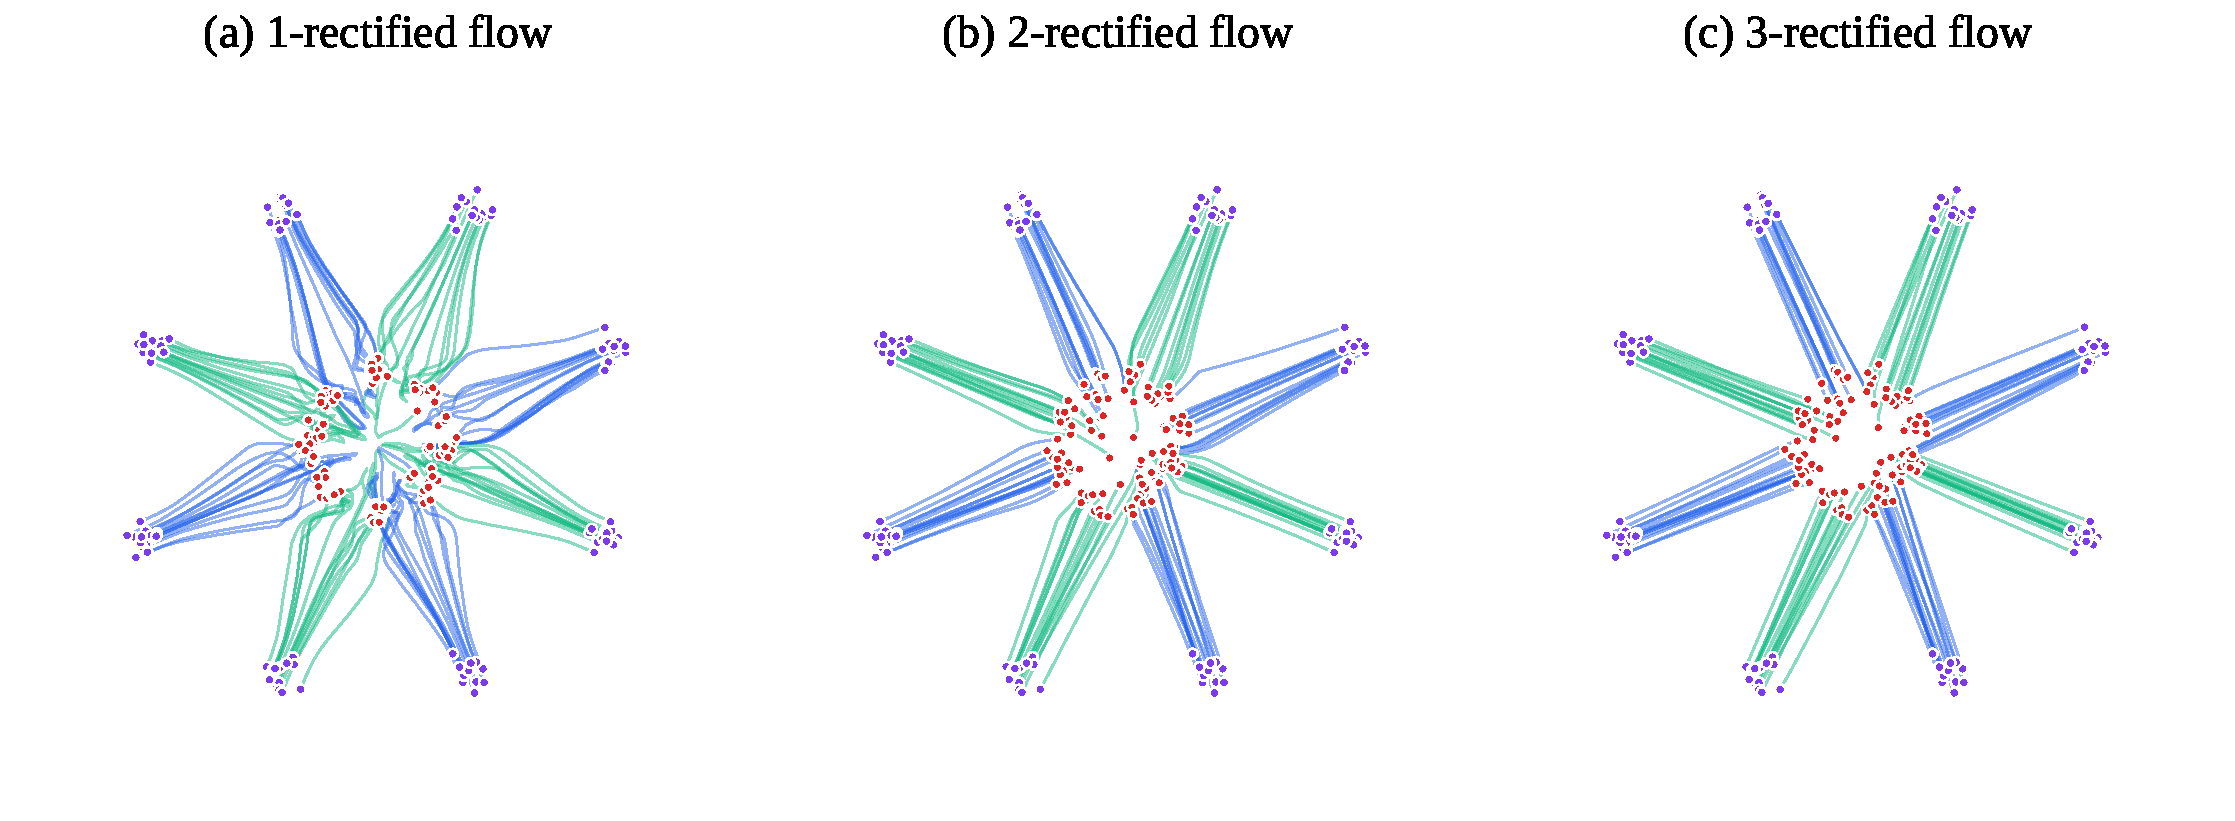
\includegraphics[width=\textwidth]{Images/PartB/rectified_flow_trained.pdf}
    \caption{\textbfs{Illustration of \texttt{Reflow}.} Paths become progressively straighter with \texttt{Rectify} procedure.  \figcredit{Adapted from \citet{liu2022flow}.}}
    \label{fig:ill_Reflow}
\end{figure}


The FM or RF formulation with linear interpolation kernels, together with the \texttt{Reflow} procedure, provides a simpler training objective and a practical method for refining stochastic couplings. For theoretical details, we refer readers to \citep{liu2022flow, liu2022rectified}.



\paragraph{III. Connection to Optimal Transport.}
Lastly, we note that straight-line couplings are not necessarily optimal in the sense of optimal transport (OT). This involves some terminology that will be introduced in \Cref{sec:ot-intro}; we therefore refer readers who are not familiar with OT to that section.

A hallmark of quadratic-cost optimal transport is that particles travel along straight lines: a particle at $\rvx_0$ moves to $\rmT(\rvx_0)$ via $\rvx_t = (1 - t)\rvx_0 + t \rmT(\rvx_0)$, where $\rmT$ is the optimal transport map. However, not every map $\rmS$ generating such straight-line paths, i.e., $\rvx_t = (1 - t)\rvx_0 + t \rmS(\rvx_0)$, is optimal. The map $\rmS$ yields the optimal flow only if it minimizes the Monge cost $\mathbb{E}[\|\rvx_0 - \rmS(\rvx_0)\|^2]$. Thus, while straight-line paths are necessary, they are not sufficient; optimality also depends on the correct endpoint map $\rmT$.

\exm{Straight Couplings Need Not Be Optimal}{
Let $p_{\text{src}} = p_{\text{tgt}} = \mathcal{N}(\bm{0}, \rmI)$. For the cost $c(\rvx, \rvy) = \|\rvx - \rvy\|^p$ with $p > 0$, the $c$-optimal coupling is the identity coupling $\pi^{*}$, where $\pi^{*}$ is the law of $(\rvx, \rvx)$ with $\rvx \sim p_{\text{src}}$.

Now consider the coupling $\pi_{\rmA}$ defined as the law of $(\rvx, \rmA \rvx)$, where $\rvx \sim p_{\text{src}}$ and $\rmA$ is a rotation matrix satisfying $\rmA^\top \rmA = \rmI$, $\det(\rmA) = 1$, $\rmA \neq \rmI$, and $-1$ is not an eigenvalue. Then $\pi_{\rmA}$ is a valid coupling of $p_{\text{src}}$ and $p_{\text{tgt}}$, and corresponds to straight-line paths between $\rvx$ and $\rmA \rvx$, but it is not $c$-optimal for any twice-differentiable strictly convex cost $c$ with invertible Hessian. The suboptimality arises from the rotational transformation. As discussed in \Cref{eq:reflow-loss-gradient}, even removing the rotation may not lead to an optimal coupling.
}

We will continue exploring the connection to OT in \Cref{subsec:ot-linear-reflow}.

\clearpage
\newpage

\newpage
\section{Closing Remarks}\label{sec:ch5_cr}
     
This chapter has illuminated the third and final foundational perspective on diffusion models, one rooted in the principles of deterministic flows. Our exploration began with Normalizing Flows (NFs), which leverage the change-of-variables formula to learn an exact, invertible mapping between a simple prior and the data distribution. We then saw this concept evolve into a continuous-time process with Neural ODEs, where a learned velocity field governs the transformation. However, this approach comes with the significant drawback of requiring costly ODE simulations within the training loop.





The modern framework of Flow Matching (FM) was presented as an elegant and efficient solution to this challenge. By pre-defining a probability path $\{p_{t}\}_t$ and a corresponding velocity field that satisfies the continuity equation, FM establishes a clear target for the ODE flow. Crucially, just as we saw in the variational and score-based views, FM employs a powerful conditioning trick. This transforms the intractable problem of matching the marginal velocity field into a simple and tractable regression against a known conditional velocity, making training entirely simulation-free. This perspective recasts diffusion models themselves as a special case of learning a deterministic flow to transport a Gaussian prior to the data distribution.




With the introduction of the flow-based view, our survey of the three conceptual pillars of diffusion modeling is now complete. Throughout this journey, a remarkable pattern has emerged: each framework, despite its unique origins in VAEs, EBMs, or NFs, has converged on a continuous-time generative process and has relied on a conditioning strategy to enable tractable learning.

In the next chapter, we will finally synthesize these parallel threads into a single, unified framework. We will:
\begin{enumerate}
    \item Formally demonstrate that the variational, score-based, and flow-based perspectives are not merely analogous but are mathematically equivalent at a fundamental level.
    \item Show how the Fokker-Planck equation serves as the universal law governing density evolution across all three views, revealing that they are simply different lenses for describing the same core generative principle.
\end{enumerate}

This unified lens will provide a complete and systematic understanding of the modern diffusion paradigm. 




\chapter{扩散模型的统一与系统性视角}\label{ch:all-equivalent} 

\epigraph{
    \textit{数学是给不同事物起相同名字的艺术。
}}{Henri Poincaré}

本章提出一个系统性的视角，将基于变分、基于分数和基于流的视角纳入一个连贯的图景之中。尽管这些方法的出发点（直觉）各不相同，但它们都收敛到现代扩散方法背后相同的核心机制。在 \Cref{ch:variational,ch:score-based,ch:score-sde,ch:flow-based} 的基础上，我们观察到一个共同的配方：定义一个前向腐蚀过程以追踪一条边缘分布的路径，然后学习一个随时间变化的向量场，沿着这条路径将一个简单的先验传输到数据分布。

所有视角中的一个关键要素是 \Cref{sec:conditional-trick} 中介绍的条件化技巧，它将一个难以处理的边缘目标转化为一个可处理的条件目标，从而带来稳定且高效的训练。

在 \Cref{sec:elucidating} 中，我们以系统的方式分析训练目标，识别其本质组件，并阐明损失函数在基于变分、基于分数和基于流的视角下是如何构造的。


\Cref{sec:equivalent-parametrizations} 表明，任何形如 $\rvx_t = \alpha_t \rvx_0 + \sigma_t \beps$ 的前向仿射噪声注入都可以等价地转化为标准的线性调度 $\rvx_t = (1 - t)\rvx_0 + t\beps$。此外，常见的参数化方式（如噪声预测、干净数据预测、分数预测和速度预测）在梯度层面上是可以相互替换的。因此，噪声调度与参数化的选择都遵循相同的建模原则。



最后，\Cref{sec:comparison-connection} 对全章讨论进行总结，并指出其统辖法则：Fokker–Planck 方程。无论被视为变分方案（离散时间去噪）、基于分数的方法（SDE 表述）还是基于流的方法（ODE 表述），每一种都构造了一个生成器，其边缘分布遵循相同的密度演化。因此，Fokker–Planck 方程是三种视角共同遵循的普适约束，差异仅体现在参数化和训练目标上。



\newpage

\section{条件化技巧：扩散模型的秘密武器}\label{sec:conditional-trick}
到目前为止，我们已经从三个看似截然不同的源头探讨了扩散模型：基于变分、基于分数和基于流的视角。每一种最初都由不同的目标所驱动，并导出了各自的训练目标（在固定 $t$ 下）：
\begin{itemize}
    \item \textbfs{变分视角：} 学习一个参数化密度 $p_{\bm{\phi}}(\mathbf{x}_{t-\Delta t}|\mathbf{x}_t)$，通过最小化以下目标来逼近 oracle 反向转移 $p(\mathbf{x}_{t-\Delta t}|\mathbf{x}_t)$：
    \[
    \mathcal{J}_{\text{KL}}(\bm{\phi}) := \mathbb{E}_{p_t(\mathbf{x}_t)}\left[
        \mathcal{D}_{\mathrm{KL}}\big(p(\mathbf{x}_{t-\Delta t}|\mathbf{x}_t) \| p_{\bm{\phi}}(\mathbf{x}_{t-\Delta t}|\mathbf{x}_t)\big)
    \right];
    \]
    \item \textbfs{基于分数的视角：} 学习一个分数模型 $\rvs_{\bm{\phi}}(\rvx_t, t)$，通过以下目标来逼近边缘分数 $\nabla_{\rvx} \log p_t(\rvx_t)$：
    \[
    \mathcal{J}_{\text{SM}}(\bm{\phi}) := \mathbb{E}_{p_t(\rvx_t)}\left[
       \left\| \rvs_{\bm{\phi}}(\rvx_t, t) - \nabla_{\rvx} \log p_t(\rvx_t) \right\|_2^2
    \right];
    \]
    \item \textbfs{基于流的视角：} 学习一个速度模型 $\rvv_{\bm{\phi}}(\rvx_t, t)$，通过最小化以下目标来匹配 oracle 速度 $\rvv_t(\rvx_t)$（例如由 \Cref{eq:marginal-oracle-velocity} 定义）：
    \[
    \mathcal{J}_{\text{FM}}(\bm{\phi}) := \mathbb{E}_{p_t(\rvx_t)} \left[
        \left\| \rvv_{\bm{\phi}}(\rvx_t, t) - \rvv_t(\rvx_t) \right\|_2^2
    \right].
    \]
\end{itemize}

乍看之下，这些目标似乎无从下手，因为它们都需要获取在一般情形下根本不可知的 oracle 量。但接下来出现了令人兴奋的转折：每种方法都独立地得到了解决该问题的同一种优雅方案：\emph{以数据 $\rvx_0$ 为条件}。这一技巧将每一个难以处理的训练目标都转化为可处理的目标。



这种优雅的“条件化技巧”将目标改写为关于已知高斯条件分布 $p_t(\rvx_t | \rvx_0)$ 的期望，从而得到梯度等价的闭式回归目标和可处理的训练目标：
\begin{itemize}
    \item \textbfs{变分视角}（\Cref{eq:kl-matching}）\textbfs{：}
    \[
    \mathcal{J}_{\text{KL}}(\bm{\phi}) = \underbrace{\mathbb{E}_{\rvx_0} \mathbb{E}_{p_t(\rvx_t|\rvx_0)} \left[
        \mathcal{D}_{\mathrm{KL}}\big(p(\rvx_{t-\Delta t}|\rvx_t, \rvx_0) \| p_{\bm{\phi}}(\rvx_{t-\Delta t}|\rvx_t)\big)
    \right]}_{\mathcal{J}_{\text{CKL}}(\bm{\phi})} + C;
    \]    
    \item \textbfs{基于分数的视角}（\Cref{eq:score-matching}）\textbfs{：}
    \[
    \mathcal{J}_{\text{SM}}(\bm{\phi}) = \underbrace{\mathbb{E}_{\rvx_0} \mathbb{E}_{p_t(\rvx_t|\rvx_0)} \left[
        \left\| \rvs_{\bm{\phi}}(\rvx_t, t) - \nabla_{\rvx_t} \log p_t(\rvx_t | \rvx_0) \right\|_2^2
    \right]}_{\mathcal{J}_{\text{DSM}}(\bm{\phi})} + C;
    \]
    \item \textbfs{基于流的视角}（\Cref{eq:fm-cfm}）\textbfs{：}
    \[
    \mathcal{J}_{\text{FM}}(\bm{\phi}) = \underbrace{\mathbb{E}_{\rvx_0} \mathbb{E}_{p_t(\rvx_t|\rvx_0)} \left[
        \left\| \rvv_{\bm{\phi}}(\rvx_t, t) - \rvv_t(\rvx_t | \rvx_0) \right\|^2
    \right]}_{\mathcal{J}_{\text{CFM}}(\bm{\phi})} + C.
    \]
\end{itemize}
为了建立统一的视角，接下来我们以系统的方式重新审视条件 KL、分数和速度目标。关键在于，这些目标不仅可处理，而且与它们各自的原形式仅相差一个常数垂直平移。
条件版本（$\mathcal{J}_{\text{CKL}}$、$\mathcal{J}_{\text{DSM}}$、$\mathcal{J}_{\text{CFM}}$）与原版本（$\mathcal{J}_{\text{KL}}$、$\mathcal{J}_{\text{SM}}$、$\mathcal{J}_{\text{FM}}$）仅相差这一平移，这不改变梯度，因而保持了优化景观。
因此，最小化解仍然与真实的 oracle 目标唯一对应，因为每一个都归结为一个最小二乘回归问题，其解恢复出对应的条件期望：
\begin{mdframed}
    \begin{align}\label{eq:three-minimizer-oracle}
\begin{aligned}
        p^*(\mathbf{x}_{t-\Delta t}|\mathbf{x}_t) &= \mathbb{E}_{\mathbf{x}_0 \sim p(\cdot|\mathbf{x}_t)} \big[p(\mathbf{x}_{t-\Delta t}|\mathbf{x}_t, \mathbf{x}_0)\big] &&= p(\mathbf{x}_{t-\Delta t}|\mathbf{x}_t), \\
    \mathbf{s}^*(\mathbf{x}_t, t) &= \mathbb{E}_{\mathbf{x}_0 \sim p(\cdot|\mathbf{x}_t)} \big[\nabla_{\mathbf{x}_t} \log p_t(\mathbf{x}_t|\mathbf{x}_0)\big] &&= \nabla_{\mathbf{x}_t} \log p_t(\mathbf{x}_t), \\
    \mathbf{v}^*(\mathbf{x}_t, t) &= \mathbb{E}_{\mathbf{x}_0 \sim p(\cdot|\mathbf{x}_t)} \big[\mathbf{v}_t(\mathbf{x}_t|\mathbf{x}_0)\big] &&= \mathbf{v}_t(\mathbf{x}_t).
\end{aligned}
\end{align}
\end{mdframed}


\exm{有限数据集上的闭式 oracle 目标}{
为了使 \Cref{eq:three-minimizer-oracle} 更具体，假设数据分布是经验测度
\[
\hat p_0=\frac{1}{N}\sum_{i=1}^N \delta_{\rvx_0^{(i)}},
\]
其中 $\{\rvx_0^{(i)}\}_{i=1}^N$ 表示有限的训练集。

在 \Cref{eq:three-minimizer-oracle} 中，记号
\[
\rvx_0 \sim p(\cdot|\rvx_t)
\]
表示我们在给定带噪观测 $\rvx_t$ 的条件下，对干净样本的后验分布求平均。等价地，对任意量 $\rvh(\rvx_0)$，
\[
\mathbb{E}_{\rvx_0 \sim p(\cdot|\rvx_t)}[\rvh(\rvx_0)]
=
\int \rvh(\rvx_0)\, p(\rvx_0|\rvx_t)\diff\rvx_0.
\]

由贝叶斯法则，
\[
p(\rvx_0|\rvx_t)
=
\frac{p_t(\rvx_t|\rvx_0)\,p_{\text{data}}(\rvx_0)}
{\int p_t(\rvx_t|\tilde{\rvx}_0)\,p_{\text{data}}(\tilde{\rvx}_0)\diff\tilde{\rvx}_0}.
\]
在标准高斯扩散前向过程下，
\[
p_t(\rvx_t|\rvx_0^{(i)})
=
\mathcal{N}\left(\rvx_t;\alpha_t \rvx_0^{(i)}, \sigma_t^2 \rmI\right),
\]
因此条件似然是显式的。然而在总体层面，后验 \(p(\rvx_0|\rvx_t)\) 仍需对完整的数据分布 \(p_{\text{data}}\) 求平均。

如果现在将 \(p_{\text{data}}\) 替换为经验测度
\[
\hat p_0=\frac{1}{N}\sum_{i=1}^N \delta_{\rvx_0^{(i)}},
\]
那么后验 \(p(\rvx_0|\rvx_t)\) 仅在训练样本上有支撑，且其在 \(\rvx_0^{(i)}\) 处的质量为
\[
p(\rvx_0=\rvx_0^{(i)}|\rvx_t)
=
\frac{p_t(\rvx_t|\rvx_0^{(i)})}
{\sum_{j=1}^N p_t(\rvx_t|\rvx_0^{(j)})}
=: w_i(\rvx_t,t),
\qquad
\sum_{i=1}^N w_i(\rvx_t,t)=1.
\]
因此上面的后验期望归结为有限和
\[
\mathbb{E}_{\rvx_0 \sim p(\cdot|\rvx_t)}[\rvh(\rvx_0)]
=
\sum_{i=1}^N w_i(\rvx_t,t)\rvh(\rvx_0^{(i)}).
\]
于是，在有限数据集的情形下，\Cref{eq:three-minimizer-oracle} 中抽象的后验平均变成了对训练集的具体加权平均，权重为 \(w_i(\rvx_t,t)\)。我们现在将这三种情形显式地写出。

\paragraph{变分视角。}
oracle 反向转移变为
\[
p^*(\rvx_{t-\Delta t}|\rvx_t)
=
\sum_{i=1}^N
w_i(\rvx_t,t) 
p(\rvx_{t-\Delta t}|\rvx_t,\rvx_0^{(i)}).
\]
这里每个条件反向核
\[
p(\rvx_{t-\Delta t}|\rvx_t,\rvx_0^{(i)})
\]
在高斯扩散下本身就有闭式表达；事实上，如引理~\ref{ddpm-reverse-kernel} 所示，它是高斯的。因此真实的反向核只是显式高斯桥的后验加权混合。

\paragraph{基于分数的视角。}
类似地，oracle 分数变为
\[
\mathbf{s}^*(\rvx_t,t)
=
\sum_{i=1}^N
w_i(\rvx_t,t) 
\nabla_{\rvx_t}\log p_t(\rvx_t|\rvx_0^{(i)}).
\]
条件分数是显式的：
\[
\nabla_{\rvx_t}\log p_t(\rvx_t|\rvx_0^{(i)})
=
-\frac{\rvx_t-\alpha_t\rvx_0^{(i)}}{\sigma_t^2}.
\]
因此，
\[
\mathbf{s}^*(\rvx_t,t)
=
-\frac{1}{\sigma_t^2}
\left(
\rvx_t-\alpha_t\sum_{i=1}^N w_i(\rvx_t,t) \rvx_0^{(i)}
\right).
\]
所以边缘分数从带噪样本指向训练样本的后验加权平均。

\paragraph{基于流的视角。}
同样的现象也出现在流匹配中：
\[
\mathbf{v}^*(\rvx_t,t)
=
\sum_{i=1}^N
w_i(\rvx_t,t) 
\mathbf{v}_t(\rvx_t|\rvx_0^{(i)}).
\]
同样，这些构建模块是显式的。相应的条件速度场具有闭式形式：
\[
\mathbf{v}_t(\rvx_t|\rvx_0^{(i)})
=
{\alpha}'_t \rvx_0^{(i)}
+
\frac{{\sigma}'_t}{\sigma_t}\bigl(\rvx_t-\alpha_t\rvx_0^{(i)}\bigr).
\]
因此 oracle 速度也是数据集上显式的后验加权平均。

综合起来，这些公式表明：在有限数据集上，所有三个 oracle 目标都归结为闭式条件量的显式后验加权平均。
}

这种共同的条件化重构并非巧合：它通过使训练变得可处理，揭示了一种深刻的统一性。变分扩散、基于分数的 SDE 和流匹配只是同一原理的不同侧面。三种视角，一个洞见，优雅地联系在一起。我们将在本章余下部分继续探讨它们的等价性。

\newpage
\clearpage

\section{阐释扩散模型训练损失的路线图
}\label{sec:elucidating}

本节构建一个关于扩散模型训练损失的系统视角。
在 \Cref{subsec:four-predictions} 中，我们将标准的三个目标扩展为更广泛的四种参数化集合，说明它们如何从不同的建模视角中产生。
在 \Cref{subsec:summary-disentagle} 中，我们将这些结果提炼为一个解耦扩散目标结构的通用框架，为 \Cref{sec:equivalent-parametrizations} 中的等价性结论奠定基础。




\subsection{扩散模型中的四种常见参数化}\label{subsec:four-predictions}
除非另有说明，本节中我们考虑前向扰动核
\[
p_t(\mathbf{x}_t|\mathbf{x}_0) = \mathcal{N}\left(\mathbf{x}_t; \alpha_t \mathbf{x}_0, \sigma_t^2 \mathbf{I} \right),
\]
其中 $\mathbf{x}_0 \sim p_{\mathrm{data}}$，如 \Cref{eq:forward_kernel} 所定义。



设 $\omega: [0, T] \to \mathbb{R}_{>0}$ 表示一个正的时间加权函数。
四种标准参数化（噪声 $\bm{\epsilon}_{\bm{\phi}}$、干净数据 $\rvx_{\bm{\phi}}$、分数 $\rvs_{\bm{\phi}}$ 和速度 $\rvv_{\bm{\phi}}$），连同它们各自的最小化解 $\bm{\epsilon}^*$、$\rvx^*$、$\rvs^*$ 和 $\rvv^*$，为清晰起见并便于后续讨论，总结如下。

\paragraph{变分视角。} 基于 DDPM 中的 KL 散度（见 \Cref{subsec:ddpm-prediction,subsec:connection-vdm}），这一方法归结为预测产生 $\mathbf{x}_t$ 的期望噪声，或预测 $\mathbf{x}_t$ 所由扰动的期望干净信号。
\begin{enumerate}
    \item \textbfs{$\beps$-预测（噪声预测）} \citep{ho2020denoising}：
    \begin{equation}\label{eq:noise-def}
        \bm{\epsilon}_{\bm{\phi}}(\mathbf{x}_t,t) \approx \mathbb{E}[\bm{\epsilon}|\mathbf{x}_t]=\bm{\epsilon}^*(\rvx_t, t)
    \end{equation}
    其训练目标为
    \[
        \mathcal{L}_{\text{noise}}(\bm{\phi}) := \mathbb{E}_t \left[\omega(t) \mathbb{E}_{\mathbf{x}_0, \bm{\epsilon}} \left\| \bm{\epsilon}_{\bm{\phi}}(\mathbf{x}_t,t) - \bm{\epsilon} \right\|_2^2 \right].
    \]
    这里 $\beps^*$ 表示为获得给定 $\rvx_t$ 而注入的平均噪声。

    \item \textbfs{$\rvx$-预测（干净数据预测）} \citep{kingma2021variational,karras2022elucidating,song2023consistency}：
    \begin{equation}\label{eq:clean-def}
        \mathbf{x}_{\bm{\phi}}(\mathbf{x}_t,t) \approx \mathbb{E}[\mathbf{x}_0|\mathbf{x}_t]=\rvx^*(\rvx_t, t)
    \end{equation}
    其训练目标为
    \[
        \mathcal{L}_{\text{clean}}(\bm{\phi}) := \mathbb{E}_t \left[\omega(t) \mathbb{E}_{\mathbf{x}_0, \bm{\epsilon}} \left\| \mathbf{x}_{\bm{\phi}}(\mathbf{x}_t,t) - \mathbf{x}_0 \right\|_2^2 \right].
    \]
    这里 $\rvx^*$ 表示给定带噪观测 $\rvx_t$ 时所有合理干净猜测的平均。
\end{enumerate}

\paragraph{基于分数的视角。} 预测噪声水平 $t$ 处的分数函数，它指向将 $\mathbf{x}_t$ 去噪回所有可能产生它的干净样本的平均方向：
\begin{enumerate}
    \item[3.]  \textbfs{分数预测} \citep{song2019generative,song2020score}：
    \begin{equation}\label{eq:score-def}
        \mathbf{s}_{\bm{\phi}}(\mathbf{x}_t,t) \approx \nabla_{\mathbf{x}_t} \log p_t(\mathbf{x}_t) = \mathbb{E}\left[\nabla_{\mathbf{x}_t} \log p_t(\mathbf{x}_t|\mathbf{x}_0) |\mathbf{x}_t\right] = \rvs^*(\rvx_t, t)
    \end{equation}
    其训练目标为
    \[
        \mathcal{L}_{\text{score}}(\bm{\phi}) := \mathbb{E}_t \left[\omega(t) \mathbb{E}_{\mathbf{x}_0, \bm{\epsilon}} \left\| \mathbf{s}_{\bm{\phi}}(\mathbf{x}_t,t) - \nabla_{\mathbf{x}_t} \log p_t(\mathbf{x}_t|\mathbf{x}_0) \right\|_2^2 \right],
    \]
    其中条件分数满足 $\nabla_{\mathbf{x}_t} \log p_t(\mathbf{x}_t|\mathbf{x}_0) = -\frac{1}{\sigma_t} \bm{\epsilon}$。
\end{enumerate}


\paragraph{基于流的视角。} 预测数据随着 $\mathbf{x}_t$ 演化时的瞬时平均速度：
\begin{enumerate}
    \item[4.] \textbfs{$\rvv$-预测（速度预测）} \citep{lipman2022flow,liu2022rectified,salimans2021progressive,albergo2023stochastic}：
    \begin{equation}\label{eq:velocity-def}
        \mathbf{v}_{\bm{\phi}}(\mathbf{x}_t, t) \approx \mathbb{E}\left[\left. \frac{\diff  \mathbf{x}_t}{\diff  t} \right| {\mathbf{x}_t}\right] =\rvv^*(\rvx_t, t)
    \end{equation}
    其训练目标为
    \[
        \mathcal{L}_{\text{velocity}}(\bm{\phi}) := \mathbb{E}_t \left[\omega(t) \mathbb{E}_{\mathbf{x}_0, \bm{\epsilon}} \left\| \mathbf{v}_{\bm{\phi}}(\mathbf{x}_t,t) - \rvv_t(\rvx_t | \rvx_0,\bm{\epsilon}) \right\|_2^2 \right],
    \]
    其中条件速度为 $\rvv_t(\rvx_t|\rvx_0,\bm{\epsilon}) = \alpha_t' \mathbf{x}_0 + \sigma_t' \bm{\epsilon}$。

    这里 $\rvv^*$ 表示穿过观测点 $\rvx_t$ 的平均速度向量。
\end{enumerate}


基于 \Cref{eq:three-minimizer-oracle} 的洞见，所有四种预测类型最终都旨在近似形如“给定观测 $\mathbf{x}_t$ 时的平均噪声、干净数据、分数或速度”的条件期望。









\subsection{解耦扩散模型的训练目标}\label{subsec:summary-disentagle}
如 \Cref{subsec:four-predictions} 所示，四种预测类型的目标函数通常共享以下模板形式，用于扩散模型训练：
% \begin{align}    \label{eq:general-dm-loss-D}
% \begin{aligned}
%    &\mathcal{L}(\bm{\phi}):=\\ &\mathbb{E}_{\rvx_0, \bm{\epsilon}}\int_{0}^{T} \underbrace{\eqnmarkbox[OliveGreen]{wgt}{\omega(t)} \eqnmarkbox[NavyBlue]{tsample}{p_{\text{time}}(t)}}_{\text{time weighting}}\underbrace{\norm{ \eqnmarkbox[Plum]{target}{\mathrm{NN}_{\bm{\phi}}}(\eqnmarkbox[Pink]{para}{\rvx_t}, t) - \eqnmarkbox[Plum]{target}{(A_t \rvx_0 + B_t \bm{\epsilon}) }}_2^2}_{\text{squared $\ell_2$ part}}\diff t.
% \end{aligned}
% \end{align}

\begin{align}    \label{eq:general-dm-loss-D}
\begin{aligned}
   \mathcal{L}(\bm{\phi}):=\mathbb{E}_{\rvx_0, \bm{\epsilon}} \underbrace{\eqnmarkbox[NavyBlue]{tsample}{\mathbb{E}_{p_{\text{time}}(t)}}}_{\substack{\text{time} \\ \vspace{0.5cm} \text{distribution}}}\Big[ \underbrace{\eqnmarkbox[OliveGreen]{wgt}{\omega(t)}}_{\substack{\text{time} \\ \vspace{0.5cm}\text{weighting}}}\underbrace{\norm{ \eqnmarkbox[Plum]{target}{\mathrm{NN}_{\bm{\phi}}}(\eqnmarkbox[Pink]{para}{\rvx_t}, t) - \eqnmarkbox[Plum]{target}{(A_t \rvx_0 + B_t \bm{\epsilon}) }}_2^2}_{\text{MSE part}}\Big].
\end{aligned}
\end{align}



这里，为了提升训练效率并优化扩散模型的学习流程，几个关键的设计选择至关重要~\citep{karras2022elucidating,lu2024simplifying}：
\begin{enumerate}
    \item[(A)] 通过 $\alpha_t$ 和 $\sigma_t$ 决定前向过程中 $\eqnmarkbox[Pink]{para}{\rvx_t}$ 的噪声调度；
    \item[(B)] $\eqnmarkbox[Plum]{target}{\mathrm{NN}_{\bm{\phi}}}$ 的预测类型及其对应的回归目标 $\eqnmarkbox[Plum]{target}{(A_t \rvx_0 + B_t \bm{\epsilon}) }$；
    \item[(C)] 时间加权函数 $\eqnmarkbox[OliveGreen]{wgt}{\omega(\cdot)} \colon [0,T] \to \mathbb{R}_{\geq 0}$；
    \item[(D)] 时间分布 $\eqnmarkbox[NavyBlue]{tsample}{p_{\text{time}}}$。
\end{enumerate}

我们在此详细阐述这四个组件，以此作为后续各节讨论的路线图。

\paragraph{(A) 噪声调度 $\alpha_t$ 与 $\sigma_t$。}
用户可以灵活选择适合其应用的调度，常见示例总结于 \Cref{tb:interpolant_instances}。重要的是，正如我们将在 \Cref{eq:fm-general-affine-formula,eq:any-to-trig} 中证明的，所有形如 $\mathbf{x}_t = \alpha_t \mathbf{x}_0 + \sigma_t \bm{\epsilon}$ 的仿射流在数学上都是等价的。具体而言，任何此类插值都可以通过适当的时间重参数化和空间缩放，转化为规范的线性调度（$\alpha_t = 1 - t$，$\sigma_t = t$）或三角调度（$\alpha_t = \cos t$，$\sigma_t = \sin t$）。


\paragraph{(B) 参数化 $\mathrm{NN}_{\bm{\phi}}$ 与训练目标 $A_t \rvx_0 + B_t \bm{\epsilon}$。}  用户可以灵活选择模型的预测目标：干净信号、噪声、分数或速度预测。如 \Cref{subsec:four-predictions} 所详述，所有这些预测类型都共享如下形式的共同回归目标
\[
    \text{Regression Target} = A_t \mathbf{x}_0 + B_t \bm{\epsilon},
\]
其中系数 $A_t$ 和 $B_t$ 既取决于所选的预测类型，也取决于调度 $(\alpha_t, \sigma_t)$。这些关系总结于 \Cref{tb:A_t-B_t-parametrizations}。

尽管这四种参数化看起来不同，我们将在 \Cref{eq:predictions-equivalence} 中证明，它们可以通过简单的代数操作相互转化。此外，我们还将在 \Cref{eq:s-e-x-v-equi} 中证明，\Cref{eq:general-dm-loss-D} 中的 $\ell_2$ 平方损失项在所有预测类型之间保持梯度等价，仅相差一个（$\omega(t) p_{\mathrm{time}}(t)$ 之外的）时间加权因子，该因子仅由噪声调度 $(\alpha_t, \sigma_t)$ 决定。



\begin{table}[th]
  \caption{不同参数化之间关系的总结。
四种参数化在数学上相互等价，可以通过简单的代数变换相互转换。
}
  \small
  \centering
  \resizebox{0.48\textwidth}{!}{
  \begin{tabular}{ccc}
     \toprule
      回归目标 =    &  \multicolumn{2}{c}{$A_t\rvx_0 + B_t \bm{\epsilon}$} \\
              &   $A_t$   & $B_t$ \\
       \midrule
    干净数据 & $1 $   & $0$ \\
      噪声 & $0$   &  $1$\\
    条件分数 & $0 $   &  -$\frac{1}{\sigma_t}$ \\
     条件速度 & $\alpha_t' $   &  $\sigma_t'$ \\
 \bottomrule
  \end{tabular}
  }
  \label{tb:A_t-B_t-parametrizations}
\end{table}



\paragraph{(C) 时间分布 $p_{\text{time}}(t)$。} 由于训练损失是关于 $t$ 的期望，从 $p_{\mathrm{time}}(t)$ 中采样时间在数学上等价于用 $p_{\mathrm{time}}(t)$ 对每个 $t$ 的 MSE 进行加权；这一因子可以被吸收到现有的时间加权 $\omega(t)$ 之中\footnote{我们关于时间的总体目标是一个如下形式的积分
\[
\mathcal{L} = \int_{0}^{T} \omega(t)\mathtt{mse}(t)\diff t,
\]
其中 $\mathtt{mse}(t)$ 表示每个 $t$ 的类 MSE 项。
如果训练时从 $t\sim p_{\mathrm{time}}(t)$ 中采样，则 $\mathcal{L}$ 的一个无偏 Monte Carlo 估计量为
\[
\widehat{\mathcal{L}} = \mathbb{E}_{t\sim p_{\mathrm{time}}} \left[ \tfrac{\omega(t)}{p_{\mathrm{time}}(t)} \mathtt{mse}(t) \right],
\]
即采样与加权可通过重要性加权互换。}。然而，经验证据\footnote{然而在实践中，我们是在一个离散的时间点集合上用小批量 SGD 来近似训练目标的。在这种近似下，$p_{\mathrm{time}}(t)$ 的不同选择会同时改变梯度的方差以及施加于每个时间步的有效权重。因此我们分别讨论 $p_{\mathrm{time}}(t)$（采样）和 $\omega(t)$（加权）。}表明，$p_{\mathrm{time}}(t)$ 的不同选择会影响性能。因此，我们分别讨论时间分布 $p_{\mathrm{time}}(t)$ 和时间加权函数 $\omega(t)$。

时间分布的一个常见选择是 $[0,T]$ 上的均匀分布~\citep{ho2020denoising,song2020score,lipman2022flow,liu2022rectified}。其他选项包括对数正态分布~\citep{karras2022elucidating}以及自适应重要性采样方法~\citep{song2021maximum,kingma2021variational}。



\paragraph{(D) 时间加权函数 $\omega(t)$。} 加权函数的一个常见选择是常数加权 $\omega \equiv 1$~\citep{ho2020denoising,karras2022elucidating,lipman2022flow,liu2022rectified}，尽管也有自适应加权方案被提出~\citep{karras2023analyzing}。$\omega(t)$ 的某些选择能将 \Cref{eq:general-dm-loss-D} 转化为负对数似然的更紧上界，从而有效地将目标重新表述为最大似然训练。$\omega(t)$ 的著名加权方案包括令 $\omega(t) = g^2(t)$~\citep{song2021maximum}，其中 $g$ 是 \Cref{eq:sde_forward} 中前向 SDE 的扩散系数。其他方法使用信噪比（SNR）加权~\citep{kingma2021variational}或单调加权函数~\citep{kingma2023understanding}，其中 $\omega(t)$ 是时间的一个单调函数。

在这些选择中，单调加权尤其有趣：它不仅仅是对训练损失的一种重加权，还具有清晰的变分解释。特别地，\citet{kim2022soft,kingma2023understanding} 证明，在单调性条件下，扩散目标等价于（相差一个可加常数）高斯增强数据上的平均 ELBO。

\subparagraph{单调加权与带数据增强的 ELBO 视角。}
我们现在解释这一解释。在加权满足单调性条件下，扩散目标等价于（相差一个可加常数）\emph{高斯噪声增强数据}上的平均 ELBO。将目标改写为共同的加权损失形式后，这一解释取决于噪声水平上诱导出的加权，而非具体的参数化。因此，下文我们使用 $\beps$-参数化纯粹作为一种方便的记号。

出发点是上文建立的加权损失形式。设
$\lambda_t := \log(\alpha_t^2/\sigma_t^2)$ 表示对数信噪比。通过从 $t$ 到 $\lambda$ 的变量替换，扩散目标可以写成
\[
\mathcal{L}_\omega(\rvx_0)
= \frac{1}{2}
\int_{\lambda_{\min}}^{\lambda_{\max}}
\omega(\lambda) 
\E_{\beps}\!\left[
\|\beps_{\bm{\phi}}(\rvx_\lambda,\lambda)-\beps\|_2^2
\right]
\diff\lambda,
\]
其中 $\omega(\lambda)$ 是有效加权函数。在总体目标层面，损失仅依赖于 $\omega(\lambda)$ 和两个端点，而不依赖于它们之间的噪声调度。

关键一步是将每个水平的去噪误差与一个全局变分量联系起来。回顾变分视角下 DDPM 的 ELBO 表述（\Cref{eq:ddpm-elbo,eq:ddpm-diffusion}），完整的负 ELBO 包含一组在所有噪声水平上比较前向过程与反向过程的 KL 项。我们现在将这一比较限制在扩散路径从噪声水平 $t$ 到终端时刻 $T$ 的剩余部分，并且不失一般性地取 $T=1$。对每个 $t \in [0,1]$，定义
\begin{equation}\label{eq:partial-chain-kl}
L(t;\rvx_0)
:=
\mathcal{D}_{\mathrm{KL}}\!\big(
  p(\rvx_{t:1} |\rvx_0)
  \;\|\;
  p_{\bm{\phi}}(\rvx_{t:1})
\big),
\end{equation}
其中 $\rvx_{t:1} := \{\rvx_s\}_{s \in [t,1]}$ 表示从水平 $t$ 到终端水平的连续时间随机路径，$p(\rvx_{t:1} |\rvx_0)$ 是给定 $\rvx_0$ 时该部分上前向过程的路径测度，而 $p_{\bm{\phi}}(\rvx_{t:1})$ 是所学反向模型对应的路径测度。这是将 $\mathcal{L}_{\mathrm{diffusion}}$（\Cref{eq:ddpm-diffusion}）中的求和限制到步骤 $i \geq t$ 的连续时间类比。在 $t = 0$ 时，$L(0;\rvx_0)$ 相差一个可加常数恢复出完整的负 ELBO；在 $t = 1$ 时，只剩下终端的不匹配。

直观上，$L(t;\rvx_0)$ 度量的是生成模型在必须从腐蚀水平 $t$ 开始反转前向过程时所付出的变分代价：对于大的 $t$，大部分腐蚀已经发生，剩余代价很小；对于小的 $t$，模型必须顾及几乎完整的反向过程，因此代价很大。

可以证明，这一代价随 $t$ 变化的速率恰好是每个水平的去噪误差：
\[
\frac{\diff}{\diff t}L(t;\rvx_0)
=
\frac{1}{2}\frac{\diff\lambda_t}{\diff t} 
\E_{\beps}\!\left[
\|\beps_{\bm{\phi}}(\rvx_t,t)-\beps\|_2^2
\right].
\]
这一恒等式揭示了每个噪声水平处的去噪损失并非一个孤立的回归目标，而是 \Cref{eq:partial-chain-kl} 中全局变分代价的瞬时变化率。代入加权损失并应用分部积分，可将导数从 $L$ 转移到加权函数上：
\[
\mathcal{L}_\omega(\rvx_0)
=
\int_0^1
\frac{\diff}{\diff t} \omega(\lambda_t)\;
L(t;\rvx_0) \diff t
+ \text{常数}.
\]
如果 $\omega(\lambda_t)$ 关于 $t$ 单调递增（等价地，关于 $\lambda$ 单调递减），则
$\frac{\diff}{\diff t} \omega(\lambda_t)\ge 0$，并且可以被归一化为噪声水平上的一个概率分布 $p_\omega(t)$。目标变为
\[
\mathcal{L}_\omega(\rvx_0)
=
\E_{t\sim p_\omega}\!\big[L(t;\rvx_0)\big]+ \text{常数}.
\]
由于 $L(t;\rvx_0)$ 相差一个可加常数就是与高斯扰动样本 $\rvx_t$ 相关的负 ELBO，单调加权具有一种简单的数据增强解释：扩散目标等价于在噪声增强数据上最大化平均 ELBO，其中增强强度按 $p_\omega$ 分布。因此，加权函数不仅仅是损失中的一个抽象系数；它决定了训练如何在不同腐蚀水平之间分配。这使目标更具可解释性，也有助于阐明为何加权的选择会同时影响优化和模型在学习中所关注的结构。


\paragraph{结论。}
就我们的目的而言，主要的经验是：扩散训练中许多表面上看起来是设计选择的东西，都可以通过它们如何重塑目标中噪声水平上的有效加权来理解。这一加权反过来既影响实践中的优化景观，又在特殊情形（如单调加权）下影响损失的变分解释。




%%%%%%%%%%%%%%%%%%%%%%%%%%%%%%%%%%%%%%%%%%%%%%%%%%%%%%%%%%%%%%%%%%%%%%%%%
\clearpage
\newpage
%%%%%%%%%%%%%%%%%%%%%%%%%%%%%%%%%%%%%%%%%%%%%%%%%%%%%%%%%%%%%%%%%%%%%%%%%%%






\section{扩散模型中的等价性}\label{sec:equivalent-parametrizations}

\Cref{subsec:four-predictions} 中引入的四种预测类型稍后将证明（\Cref{subsec:four-equiv-para}）在梯度最小化下是等价的。
随后我们在 \Cref{subsec:all-flows-are-equiv} 中拓宽这一视角，说明不同的前向噪声调度可通过简单的时间和空间缩放相互联系。





\subsection{四种预测类型相互等价}\label{subsec:four-equiv-para}
我们首先分析 \Cref{eq:general-dm-loss-D} 中组件 (B) 的设计选择。

我们已经看到，四种预测类型并非独立的选择，而是同一个底层量的不同视角。
例如，噪声预测与干净数据预测直接相关（\Cref{subsec:ddpm-prediction}），分数预测与噪声预测也是如此（\Cref{sec:SMLD}）。
这种反复出现的模式指向一个更深的原理：所有四种参数化在代数上等价，可以通过简单的变换相互转化。
为使这一联系精确化，我们陈述如下命题，如 \Cref{fig:equiv-parametrizations} 所示，参见~\citep{kingma2021variational}。
\proppp{参数化的等价性}{equi-para}{
设最小化各自目标的最优预测为
\[
\bm{\epsilon}^*(\rvx_t,t) , \quad \rvx^*(\rvx_t,t), \quad \rvs^*(\rvx_t,t) , \quad \rvv^*(\rvx_t,t),
\]
分别对应噪声、干净数据、分数和速度参数化。它们满足如下等价关系：
\begin{equation}\label{eq:predictions-equivalence}
\begin{aligned}
\bm{\epsilon}^*(\rvx_t,t) &= -\sigma_t \rvs^*(\rvx_t,t), \\
\rvx^*(\rvx_t,t) &= \frac{1}{\alpha_t} \rvx_t
+ \frac{\sigma_t^2}{\alpha_t} \rvs^*(\rvx_t,t), \\
\rvv^*(\rvx_t,t) &= \alpha_t' \rvx^* + \sigma_t' \bm{\epsilon}^* 
= f(t)\rvx_t - \frac{1}{2} g^2(t)\rvs^*(\rvx_t,t).
\end{aligned}
\end{equation}
这里，$f(t)$ 和 $g(t)$ 通过引理~\ref{forward-sde} 与 $\alpha_t$ 和 $\sigma_t$ 相联系。
此外，这些最小化解满足 \Cref{eq:noise-def,eq:clean-def,eq:score-def,eq:velocity-def} 中给出的恒等式。
}{证明类似于定理~\ref{dsm-minimizer}，后者分析了 DSM 目标下各种匹配损失的全局最优解。详见 \Cref{app-sec:equiv-para}。
}


\begin{figure}[th]
    \centering
\begin{tikzpicture}[
    node distance=2cm and 3cm,
    box/.style={rectangle,draw,fill=gray!10,minimum width=2.5cm,minimum height=1cm,align=center},
    arr/.style={-{Latex[length=3mm,width=2mm]},thick,font=\footnotesize},
    lbl/.style={draw,rounded corners,fill=white,fill opacity=1,inner sep=2pt}
  ]
  % 1) Nodes
  \node[box]            (Score)    {\textbfs{分数}};
  \node[box,right=of Score]   (Noise)    {\textbfs{噪声}};
  \node[box,below=of Noise]   (Velocity) {\textbfs{速度}};
  \node[box,below=of Score]   (Clean)    {\textbfs{干净数据}};

  % 2) Arrows on background layer
  \begin{pgfonlayer}{background}
    \draw[arr] (Score)    -- (Noise);
    \draw[arr] (Score)    -- (Clean);
    \draw[arr] (Score)    -- (Velocity);
    \draw[arr] (Noise)    -- (Velocity);
    \draw[arr] (Noise)    -- (Score);
    \draw[arr] (Clean)    -- (Score);
    \draw[arr] (Clean)    -- (Velocity);
    \draw[arr] (Velocity) -- (Clean);
    \draw[arr] (Velocity) -- (Score);
    \draw[arr] (Velocity) -- (Noise);
  \end{pgfonlayer}

  % 3) Labels (on main layer, thus on top of arrows)
  \node[lbl] at ($(Score)!0.5!(Noise)+(0,0.5)$)
    (eqlabel) {$\displaystyle \bm{\epsilon}^* = -\sigma_t\rvs^*$};
  \node[lbl] at ($(Score)!0.5!(Clean)+(-1.2,0)$)
    (xlabel) {$\displaystyle \rvx^* =\tfrac1{\alpha_t}\rvx_t + \tfrac{\sigma_t^2}{\alpha_t}\rvs^*$};
  \node[lbl] at ($(Velocity)!0.5!(Score)-(0,0.0)$)
    (vlabel) {$\displaystyle \rvv^* = f(t)\rvx_t - \tfrac12 g^2(t)\rvs^*$};
  \node[lbl] at ($(Clean)!0.5!(Noise)+(4.2,0)$)
    (vvlabel) {$\displaystyle  \rvv^*=\alpha_t'\rvx^*+\sigma_t'\bm{\epsilon}^*(\bm{\star})$};
  \node[lbl] at ($(Clean)!0.5!(Velocity)+(0,-0.4)$)
    (vvlabel) {$\displaystyle (\bm{\star})$};


\end{tikzpicture}
    \caption{\textbfs{四种参数化之间的等价关系。} $\rvv$-预测由 $\rvv^* = \alpha_t' \rvx^* + \sigma_t' \bm{\epsilon}^*$ 给出，
其中干净数据预测与 $\beps$-预测可通过
$\rvx_t = \alpha_t \rvx^* + \sigma_t \bm{\epsilon}^*$ 相互转换。
\figcredit{由作者绘制。}}
    \label{fig:equiv-parametrizations}
\end{figure}

\Cref{eq:predictions-equivalence} 在四种参数化之间（在每个 $t$ 处，给定前向加噪系数时）诱导出一种一一对应的转换
\[
\bm{\epsilon}_{\bm{\phi}}(\rvx_t,t), \quad \rvx_{\bm{\phi}}(\rvx_t,t), \quad \rvs_{\bm{\phi}}(\rvx_t,t), \quad   \rvv_{\bm{\phi}}(\rvx_t,t).
\]
在实践中，我们用某一种参数化（例如 $\bm\epsilon_{\bm\phi}$）训练单个网络。其他量则由 \Cref{eq:predictions-equivalence} 中的转换\emph{事后定义}。


\subsection{不同参数化下的 PF-ODE}\label{subsec:pf-ode-different-para} 
PF-ODE 容许若干种等价的参数化（分数、噪声、去噪、速度）。
尽管原则上可以互换，但这一选择具有实际后果：它改变了向量场的刚性、离散化误差的行为以及优化的难易程度。
对于使用高级 ODE 求解器的快速采样（见 \Cref{ch:solvers}），实践者通常采用 $\beps$ 或 $\rvx$ 预测，因为它们与求解器输入契合良好并能减少误差累积。
对于仅使用少数几次函数求值进行训练的生成器（见 \Cref{ch:fast-scratch}），$\rvx$ 或 $\rvv$ 预测通常能产生更平滑的目标以及更好的逐步一致性。


我们写出每种参数化下的 PF-ODE，并利用 \Cref{eq:predictions-equivalence} 显式地进行转换。结果汇总于如下命题。

\proppnp{不同参数化下的 PF-ODE}{pf-ode-para}{
设 $\alpha_t$ 和 $\sigma_t$ 为前向扰动调度，并记时间导数为
$\alpha_t' := \tfrac{\diff \alpha_t}{\diff t}$ 和 $\sigma_t' := \tfrac{\diff \sigma_t}{\diff t}$。
则经验 PF-ODE 容许如下等价形式
\begin{align}\label{eq:clean_pf_ode}
\begin{aligned}
    \frac{\diff \rvx(t)}{\diff t}
    &= \frac{\alpha_t'}{\alpha_t} \rvx(t)
 - \sigma_t \left(\frac{\alpha_t'}{\alpha_t}-\frac{\sigma_t'}{\sigma_t}\right)
   \bm{\epsilon}^*(\rvx(t), t) \\    
    &= \frac{\sigma_t'}{\sigma_t} \rvx(t)
 + \alpha_t \left(\frac{\alpha_t'}{\alpha_t}-\frac{\sigma_t'}{\sigma_t}\right)
   \rvx^*(\rvx(t), t) \\
    &= \frac{\alpha_t'}{\alpha_t} \rvx(t)
 + \sigma_t^{2} \left(\frac{\alpha_t'}{\alpha_t}-\frac{\sigma_t'}{\sigma_t}\right)
   \rvs^*(\rvx(t), t) \\ 
   &= \alpha_t'\rvx^*(\rvx(t), t) + \sigma_t' \beps^*(\rvx(t), t)\\
    &= \rvv^*(\rvx(t), t).
\end{aligned}
\end{align}
}
为了看清 Score SDE 的记号，我们回顾引理~\ref{forward-sde}。如果令
\[
f(t) = \frac{\alpha_t'}{\alpha_t}, 
\quad
g^2(t) = \frac{\diff}{\diff t} \big(\sigma_t^2\big) 
         - 2 \frac{\alpha_t'}{\alpha_t} \sigma_t^2
       = 2\sigma_t\sigma_t' - 2 \frac{\alpha_t'}{\alpha_t} \sigma_t^2,
\]
那么 PF-ODE 可以写成熟悉的 Score SDE 形式：
\[
\frac{\diff \rvx(t)}{\diff t}
= f(t) \rvx(t)  -  \frac{1}{2} g^2(t) \rvs^*(\rvx(t),t).
\]

为了给读者一个关于 PF-ODE 如何被离散化以进行采样的具体感受，我们将在 \Cref{sec:revisit-ddim} 中介绍一种广泛使用的基于扩散的 ODE 采样器——DDIM 方案的更新规则。这个例子将展示 Euler 离散化如何自然地与 PF-ODE 联系起来.







\subsection{所有仿射流都是等价的}\label{subsec:all-flows-are-equiv}
我们接下来分析 \Cref{eq:general-dm-loss-D} 中组件 (A) 的设计选择。

\paragraph{状态层面的等价性。}
FM~\citep{lipman2022flow} 和 RF~\citep{liu2022rectified} 中使用的一种方便的规范插值是
\[
\rvx_t^{\mathrm{FM}}=(1-t) \rvx_0+t \beps = \rvx_{0}+t(\beps-\rvx_0),
\]
其速度是常向量 $\beps-\rvx_0$。本小节的要点是，这一选择表面上的简洁性并非本质所在：任何仿射插值
\[
\rvx_t=\alpha_t \rvx_0+\sigma_t \beps
\]
都可以写成规范路径的时间重参数化和缩放版本。定义
\[
c(t):=\alpha_t+\sigma_t,
\qquad
\tau(t):=\frac{\sigma_t}{\alpha_t+\sigma_t}
\quad\big(c(t)\neq 0\big).
\]
直接的代数改写给出
\begin{align*}
\rvx_t
&=\alpha_t \rvx_0+\sigma_t \beps
\\
&=\big(\alpha_t+\sigma_t\big) \left(\frac{\alpha_t}{\alpha_t+\sigma_t}\rvx_0+\frac{\sigma_t}{\alpha_t+\sigma_t}\beps\right) \\
&=c(t) \left(\big(1-\tau(t)\big)\rvx_0+\tau(t)\beps\right)
=c(t) \rvx_{\tau(t)}^{\mathrm{FM}}.
\end{align*}
因此每条仿射路径都是规范 FM 路径在变量替换 $t\mapsto\tau(t)$ 和空间缩放 $\rvx\mapsto c(t)\rvx$ 下的像。该等式逐点成立，因此在分布意义上也成立。

对于相关的速度，对 $\rvx_t=c(t)\rvx_{\tau(t)}^{\mathrm{FM}}$ 应用链式法则：
\begin{align*}
\rvv(\rvx_t,t)
&:= \frac{\diff}{\diff t}\left(\alpha_t\rvx_0 +\sigma_t \beps\right)
\\&=\frac{\diff}{\diff t}\big(c(t)\rvx_{\tau(t)}^{\mathrm{FM}}\big)
\\
&=c'(t) \rvx_{\tau(t)}^{\mathrm{FM}}+c(t) \tau'(t) \frac{\diff}{\diff s}\rvx^{\mathrm{FM}}_{s}\bigg|_{s=\tau(t)} \\
&=c'(t) \rvx_{\tau(t)}^{\mathrm{FM}}+c(t) \tau'(t) \rvv^{\mathrm{FM}} \left(\rvx_{\tau(t)}^{\mathrm{FM}},\tau(t)\right),
\end{align*}
因为在规范路径上 $\rvv^{\mathrm{FM}}(\rvx^{\mathrm{FM}}_{\tau},\tau)=-\rvx_0+\beps$。

我们将上述推导总结为如下命题中的形式化陈述。

\proppnp{仿射流的等价性}{equiv-interpolation}{
设 $\rvx_t^{\mathrm{FM}}=(1-t)\rvx_0+t \beps$ 和 $\rvx_t=\alpha_t\rvx_0+\sigma_t\beps$，其中 $c(t):=\alpha_t+\sigma_t\neq 0$ 且 $\tau(t):=\sigma_t/(\alpha_t+\sigma_t)$。则
\begin{align}\label{eq:fm-general-affine-formula}
\begin{aligned}
\rvx_t&=c(t) \rvx_{\tau(t)}^{\mathrm{FM}},\\
\rvv(\rvx_t,t)
&=c'(t) \rvx_{\tau(t)}^{\mathrm{FM}}
 + c(t) \tau'(t) \rvv^{\mathrm{FM}} \left(\rvx_{\tau(t)}^{\mathrm{FM}},\tau(t)\right).
\end{aligned}
\end{align}
特别地，所有仿射插值在相差时间重参数化和空间缩放的意义下都是等价的。
}
\subparagraph{与三角流的等价性。}
另一种广泛使用的仿射流是三角插值~\citep{salimans2021progressive,albergo2023stochastic,lu2024simplifying}。
作为一个具体例子，我们也证明\emph{任何}仿射流都可以表示为这种形式。
三角路径定义为
\begin{align}\label{eq:trig-para}
\rvx^{\mathrm{Trig}}_u := \cos(u) \rvx_0 + \sin(u)\beps .
\end{align}
令 $R_t := \sqrt{\alpha_t^2 + \sigma_t^2}$ 并假设 $R_t>0$。选取角度 $\tau_t$ 使得
\[
\cos \tau_t = \frac{\alpha_t}{R_t},
\qquad
\sin \tau_t = \frac{\sigma_t}{R_t}.
\]
那么每个仿射插值 $\rvx_t=\alpha_t\rvx_0+\sigma_t\beps$ 都是一个经过缩放和重新计时（re-timed）的三角路径：
\begin{align}\label{eq:any-to-trig}
\rvx_t
= \alpha_t\rvx_0+\sigma_t\beps
= R_t \left(\frac{\alpha_t}{R_t}\rvx_0+\frac{\sigma_t}{R_t}\beps\right)
= R_t \rvx^{\mathrm{Trig}}_{\tau_t}.
\end{align}
数对 $(\alpha_t,\sigma_t)$ 是平面上的一个点。用 $R_t$ 归一化后它落在单位圆上，这就固定了角度 $\tau_t$ 从而固定了状态 $\rvx^{\mathrm{Trig}}_{\tau_t}$；半径 $R_t$ 给出了整体尺度。

将 $\rvx^{\mathrm{Trig}}_u$ 对 $u$ 求导得到其速度，
\[
\rvv^{\mathrm{Trig}}_u = -\sin(u) \rvx_0 + \cos(u) \beps.
\]
通过与 \Cref{eq:any-to-trig} 中相同的变量替换，这一关系为速度（类似地为其他参数化）提供了闭式转换。


综合上述讨论，我们得到如下结论：
\msg{结论}{}{无论采用何种调度 $(\alpha_t,\sigma_t)$，包括 VE、VP（如三角调度）、FM 或 RF，仿射插值都可以通过适当的时间变量替换和标量缩放相互转换。}



\paragraph{四种参数化的训练目标。}
设 $\rvx_t=\alpha_t \rvx_0+\sigma_t \beps$，其中 $\sigma_t>0$ 且 $(\alpha_t,\sigma_t)$ 可微并满足 $\alpha_t'\sigma_t-\alpha_t\sigma_t'\neq 0$。考虑 oracle 目标
\[
\beps^*(\rvx_t,t)=\E[\beps|\rvx_t],\quad 
\rvx_0^*(\rvx_t,t)=\E[\rvx_0|\rvx_t],\quad
\rvv^*(\rvx_t,t)=\E[\alpha_t'\rvx_0+\sigma_t'\beps|\rvx_t].
\]
由命题~\ref{equi-para}，它们满足
\[
\nabla_{\rvx_t}\log p_t(\rvx_t)
= -\frac{1}{\sigma_t} \beps^*(\rvx_t,t)
= \frac{\alpha_t}{\sigma_t^2} \left(\rvx_0^*(\rvx_t,t)-\frac{\rvx_t}{\alpha_t}\right),
\quad
\rvv^*=\alpha_t' \rvx_0^*+\sigma_t' \beps^*.
\]
在头部转换
\[
\rvs_{\bphi} \equiv -\frac{1}{\sigma_t} \beps_{\bphi}
\equiv \frac{\alpha_t}{\sigma_t^2} \left(\rvx_{\bphi}-\frac{\rvx_t}{\alpha_t}\right),
\]
之下，速度到分数的转换为
\[
\rvs_{\bphi}
= \frac{\alpha_t}{\sigma_t(\alpha_t'\sigma_t-\alpha_t\sigma_t')} \rvv_{\bphi}
- \frac{\alpha_t'}{\sigma_t(\alpha_t'\sigma_t-\alpha_t\sigma_t')} \rvx_t,
\]
逐样本的平方损失仅相差时间相关权重：
\begin{align}\label{eq:s-e-x-v-equi}
\begin{aligned}
\big\|\rvs_{\bphi}-\nabla_{\rvx_t}\log p_t(\rvx_t)\big\|_2^2
&=\frac{1}{\sigma_t^2} \big\|\beps_{\bphi}-\beps^*\big\|_2^2 \\
&=\frac{\alpha_t^2}{\sigma_t^4} \big\|\rvx_{\bphi}-\rvx_0^*\big\|_2^2 \\
&=\left(\frac{\alpha_t}{\sigma_t(\alpha_t'\sigma_t-\alpha_t\sigma_t')}\right)^{ 2}
\big\|\rvv_{\bphi}-\rvv^*\big\|_2^2 .
\end{aligned}
\end{align}

由命题~\ref{equiv-interpolation}，任何仿射流 $\rvx_t=\alpha_t\rvx_0+\sigma_t\beps$
都可通过 $\rvx_t=c(t)\rvx^{\mathrm{FM}}_{\tau(t)}$ 转换到规范 FM 路径，其中
$c(t)=\alpha_t+\sigma_t$ 且 $\tau(t)=\sigma_t/(\alpha_t+\sigma_t)$。求导给出
\[
\rvv_{\bphi}(\rvx_t,t)=c'(t)\rvx^{\mathrm{FM}}_{\tau(t)}
+c(t)\tau'(t)\rvv^{\mathrm{FM}}_{\bphi} \left(\rvx_{\tau(t)}^{\mathrm{FM}},\tau(t)\right),
\qquad
\rvx_{\tau(t)}^{\mathrm{FM}}=\frac{\rvx_t}{c(t)},
\]
并且同样的关系对 $\rvv^*$ 成立。因此速度损失的变换为
\begin{align*}
    &\big\|\rvv_{\bphi}(\rvx_t,t)-\rvv^*(\rvx_t,t)\big\|_2^2
\\= &\big(c(t) \tau'(t)\big)^2
\Big\|\rvv^{\mathrm{FM}}_{\bphi} \left(\frac{\rvx_t}{c(t)},\tau(t)\right)
-\big(\rvv^{\mathrm{FM}}\big)^* \left(\frac{\rvx_t}{c(t)},\tau(t)\right)\Big\|_2^2.
\end{align*}

基于上述观察，我们得到如下结论：
\msg{结论}{}{分数、噪声、干净数据和速度的训练目标在理论上仅相差由 $(\alpha_t,\sigma_t)$ 决定的时间相关权重（对速度而言，还相差一个涉及 $\rvx_t$ 的仿射头部转换）。}


\subsection{（选读）参数化与规范流的概念性分析}\label{subsec:concept-why-v-affine}
尽管我们在前几节中已经表明，所有四种参数化在数学上等价并可以相互转换，且前向仿射噪声注入流等价于规范形式
\[
\rvx_t^{\mathrm{FM}} = (1-t) \rvx_0 + t \beps,
\]
在本小节中我们提供进一步的直觉，并分析使用 $\rvv$-预测参数化与这一规范仿射流结合时的潜在优势。


本小节提出一个简单的问题：\emph{不同的参数化和调度如何塑造模型所学的内容以及我们采样的方式？} 我们从两个视角展开：
\begin{itemize}
  \item \textbfs{回归目标与调度。} 我们关注为何将 $\rvv$-预测与规范线性调度 $(\alpha_t,\sigma_t)=(1-t,t)$ 结合是自然的：它随时间保持稳定的目标尺度，并消除动力学中的曲率效应。
  \item \textbfs{对求解器的影响。} 我们考察这一参数化在概念上如何与数值积分方案相互作用，而将具体例子（如 Euler 求解器和 Heun 方法）推迟到 \Cref{subsec:ddim-different-para,subsec:dpm-heun}。
\end{itemize}

在展开之前，为避免歧义，我们区分两类速度场。\emph{条件速度}（作为可处理的训练目标）定义为
\[
\rvv_t(\rvx_t |\rvz) = \rvx_t' = \alpha_t' \rvx_0 + \sigma_t' \beps, 
\quad \text{其中 } \rvz = (\rvx_0, \beps),
\]
而\emph{oracle（边缘化）速度}（在 PF-ODE 求解的推理阶段用于移动样本）由下式给出
\[
\rvv^*(\rvx, t) = \E\big[\rvv_t(\cdot |\rvz)  \big|  \rvx_t = \rvx\big].
\]

\paragraph{视角一：为何 $(\alpha_t,\sigma_t)=(1-t,t)$ 是自然的调度。}
将 $\sigma_t:=\rho(t)$ 和 $\alpha_t:=1-\rho(t)$ 写成关于时变 $\rho(t)$ 的形式，条件速度变为
\[
\rvv_t(\rvx_t |\rvz)
=\rho'(t)(\beps-\rvx_0),
\quad\text{其中 } \rvz=(\rvx_0,\beps).
\]


\subparagraph{单位尺度的回归目标。}
对于规范调度 $\rho(t)=t$，条件速度 $\rvv_t(\cdot |\rvz)$ 满足
\begin{align}\label{eq:unit-velocity}
\mathbb{E}\left[\|\rvv_t(\cdot |\rvz)\|_2^2\right]
=\E_{\beps}\norm{\beps}_2^2+\E_{\rvx_0}\norm{\rvx_0}^2_2 = D + \underbrace{\Tr\Cov[\rvx_0]}_{\text{total variance}}+\underbrace{\norm{\E\rvx_0}^2_2}_{\text{mean}}.
\end{align}
因此期望的目标幅值关于 $t$ 是常数。在将数据标准化为零均值和单位协方差（即 $\Cov[\rvx_0]=\rmI$）之后，两个分量
$\alpha_t'\rvx_0$ 和 $\sigma_t'\beps$ 对所有 $t$ 都贡献相当，避免了端点附近的梯度爆炸/消失。
为了看清这一点，我们考虑扩散的训练目标：
\[
\mathcal{L}_{\mathrm{velocity}}(\bphi)
= \E_{t}  \E_{\rvx_0,\beps}\left[\big\|\rvv_{\bphi}(\rvx_t,t) - \rvv_t(\rvx_t|\rvz)\big\|_2^2
\right].
\]
应用链式法则，该损失关于模型参数 $\bphi$ 的梯度为
\[
\nabla_{\bphi}\mathcal{L}_{\mathrm{velocity}}(\bphi)
= 2  \E_{t}  \E_{\rvx_0,\beps} \left[
  \partial_{\bphi}\rvv_{\bphi}(\rvx_t,t)^{\top} \left(\rvv_{\bphi}(\rvx_t,t) - \rvv_t(\rvx_t|\rvz)\right)
\right].
\]
因此目标 $\|\rvv_t(\rvx_t|\rvz)\|_2$ 的尺度影响梯度稳定性：
如果在某个 $t$ 处它塌缩为 $0$（或爆炸），那么（在其他条件相同时）梯度倾向于消失（或爆炸）。采用规范选择 $\rho(t)=t$ 时，
\Cref{eq:unit-velocity} 给出一个与 $t$ 无关的目标幅值，因此不会出现由回归信号引起的端点（$t=0$ 或 $t=1$）塌缩或爆炸
（假设 $\E\|\partial_{\bphi}\rvv_{\bphi}(\rvx_t,t)\|^2$ 和任何时间权重都是受控的）。


\subparagraph{规范调度与 $\rvv$-预测的相互作用。}
在仿射路径 $\rvx_t=\alpha_t \rvx_0+\sigma_t\beps$ 下，oracle 速度分解为
\[
\rvv^*(\rvx, t)=\alpha_t' \rvx^*(\rvx,t)+\sigma_t' \beps^*(\rvx,t),
\]
其中 $\rvx^*=\E[\rvx_0|\rvx_t=\rvx]$ 且 $ \beps^*=\E[\beps|\rvx_t=\rvx]$。
在固定 $\rvx$ 下求导给出
\[
\partial_t \rvv^*
=\underbrace{\alpha_t'' \rvx^*+\sigma_t'' \beps^*}_{\text{schedule curvature}}
+ \alpha_t' \partial_t \rvx^*+\sigma_t' \partial_t \beps^*.
\]
采用线性调度 $\alpha_t=1-t,\ \sigma_t=t$ 时，曲率项消失
（$\alpha_t''=\sigma_t''=0$），因此 $\rvv^*$ 的时间变化主要反映后验演化 $(\partial_t \rvx^*,\partial_t \beps^*)$ 而非调度本身。
这一效应对于 $\rvv$-预测尤为干净：系数 $\alpha_t',\sigma_t'$
是常数（$-1$ 和 $+1$），避免了漂移中额外的随 $t$ 变化的缩放。
相比之下，分数、$\rvx_0$ 或 $\beps$ 参数化通常会引入诸如
$\sigma_t'/\sigma_t$ 或 $\alpha_t'/\alpha_t$ 这样的比值，它们即使在线性调度下也可能在端点附近剧烈变化。
因此，尽管理论上并非独有，但线性 $(1-t,t)$ 调度与 $v$-预测相结合，为 oracle 速度提供了一种特别稳定且透明的时间依赖关系。

\subparagraph{最小化条件能量。} 我们接下来采用最优传输（见 \Cref{ch:ot-eot}）的更理论化的视角。
这里，\emph{条件动能}度量条件速度沿前向路径的总期望运动，
即从 $\rvx_0$ 跨越到 $\beps$ 所需的瞬时运动（或动能耗费）总量：
\[
\mathcal K[\rho]
:=\int_0^1 \E_{\rvx_0,\beps}\!\big[\|\rvv_t(\cdot |\rvz)\|_2^2\big]\diff t
=\Big(D+\Tr\Cov[\rvx_0]+\|\E\rvx_0\|_2^2\Big)
\int_0^1 \big(\rho'(t)\big)^2\diff t.
\]
因此最小化 $\mathcal K[\rho]$ 对应于在仿射插值族
\[
\rvx_t=(1-\rho(t))\rvx_0+\rho(t)\beps.
\]
内寻找期望意义下最平滑、能量最少的路径。
在边界条件 $\rho(0)=0$ 和 $\rho(1)=1$ 下，Euler--Lagrange 方程 $\rho''(t)=0$ 给出最小化解 $\rho(t)=t$，对应于一条直的条件路径。
这意味着，在该族中所有平滑调度 $\rho$ 之中，
规范流 $\rho(t)=t$ 是从 $\rvx_0$ 移动到 $\beps$ 的最节能方式。
我们将在命题~\ref{ot-conditional-flow} 中重新讨论这一点，给出更详细的处理。


\subparagraph{关于 oracle 速度的注记。}
如果我们改为评估由边缘速度定义的能量
\[
\int_0^1 \E_{\rvx_t} \big[\|\rvv^*(\rvx_t, t)\|^2\big]\diff t,
\]
那么取 $\rvz=(\rvx_0,\beps)$ 且 $\rvv_t(\rvx_t |\rvz)=\rho'(t)(\beps-\rvx_0)$ 时，
\[
\rvv^*(\rvx, t)
=\E[\rvv_t(\cdot|\rvz)|\rvx_t=\rvx]
=\rho'(t) \E[\beps-\rvx_0|\rvx_t=\rvx];
\]
因此边缘速度的能量变为
\begin{align*}
  \int_0^1 \E_{\rvx_t\sim p_t} \big[\|\rvv^*(\rvx_t, t)\|^2_2\big]\diff t
   = \int_0^1 \E_{\rvx_t} \big[\| \rho'(t) \E[\beps-\rvx_0|\rvx_t] \|^2_2\big]\diff t  = \int_0^1 \big(\rho'(t)\big)^2 \kappa(t) \diff t,
\end{align*}
其中 $\kappa(t):=\E_{\rvx_t\sim p_t} \left[\big\|\E[\beps-\rvx_0|\rvx_t]\big\|^2_2\right]
$。

因此，\emph{边缘}最优调度 $\rho(t)$ 未必是线性的。
它为线性的充要条件是 $\kappa(t)$ 为常数；一般地，Euler–Lagrange 条件
\[
(\kappa(t)\rho'(t))' = 0  \Rightarrow  \rho'(t)\propto \frac{1}{\kappa(t)}
\]
意味着 oracle 最优调度会自适应地重参数化时间。
直观地说，$\kappa(t)$ 度量了标签 $(\beps-\rvx_0)$ 中可由 $\rvx_t\sim p_t$ 预测的部分：
oracle 流在 $\kappa(t)$ 大的地方放慢，反映 oracle 速度期望幅值大的区域；在 $\kappa(t)$ 小的地方加快。
因此，尽管条件流使用线性调度 $(1-t,t)$，
相应的边缘化（oracle）动力学一般是非线性的。



\paragraph{视角二：为何速度预测可被视为对采样是自然的。}

\subparagraph{$\rvx$-、$\beps$-、$\rvs$-预测下 PF-ODE 的半线性形式。}
在干净数据、噪声和分数参数化下，漂移项具有半线性形式（见 \Cref{eq:clean_pf_ode} 中前三个恒等式）：
\[
\frac{\diff \rvx(t)}{\diff t}= \underbrace{L(t) \rvx(t)}_{\text{linear part}} + \underbrace{\rmN_\bphi(\rvx(t),t)}_{\text{nonlinear part}},
\quad
\rmN_\bphi\in\{\rvx_{\bphi}, \beps_{\bphi}, \rvs_{\bphi}\}.
\]



当线性漂移 $L(t) \rvx(t)$ 在某些方向上驱动 $\rvx(t)$ 变化的速率与非线性部分相差悬殊时，系统就是\emph{刚性}的，这意味着漂移关于 $\rvx$ 的 Jacobian
\[
\rmJ(\rvx,t):=L(t)+\nabla_{\rvx}\rmN_\bphi(\rvx,t)
\]
的特征值的实部相差若干数量级（更大的幅值对应更快的方向）\footnote{%
设 PF–ODE 的漂移为 $\rmF(\rvx,t)=L(t) \rvx+\rmN_{\bphi}(\rvx,t)$，并假设
$\rmN_{\bphi}$ 关于 $\rvx$（局部）Lipschitz，常数为 $\mathrm{Lip}_{\rmN_{\bphi}}(t)$。
对邻近状态 $\rvx,\rvy$，
\[
\|\rmF(\rvx,t)-\rmF(\rvy,t)\|
\le \underbrace{\big(\|L(t)\|+\mathrm{Lip}_{\rmN_{\bphi}}(t)\big)}_{=:~C(t)} \|\rvx-\rvy\|.
\]
等价地，关于 $\rvx$ 的 Jacobian
\[
\rmJ(\rvx,t)=L(t)+\nabla_{\rvx}\rmN_\bphi(\rvx,t)
\]
满足 $\|\rmJ(\rvx,t)\|_{\mathrm{op}} \le C(t)$（即由 $\R^D$ 上欧氏范数诱导的算子范数）。因此 $\rmJ$ 所有特征值的实部在幅值上以 $C(t)$ 为界。
于是大的 $C(t)$ 意味着快的局部速率，所以显式求解器需要很小的步长（$h\lesssim 1/C(t)$）。}。例如，动力学可能在 $\rvx(t)$ 中同时包含“快线性”变化和“慢非线性”变化。在这种情形下，显式求解器必须采用非常小的时间步才能保持数值稳定。




为了应对这种失衡，高阶的稳定求解器通常会应用一个\emph{积分因子}，
将线性项 $L(t) \rvx$ 解析地处理，只对较慢的非线性余项进行离散化，尽管这要以额外的代数和实现复杂性为代价。\Cref{ch:solvers} 专门详细讨论这一主题。


\subparagraph{$\rvv$-预测下的 PF-ODE。} 在 $\rvv$-预测下，模型直接学习速度场并积分
\[
\frac{\diff \rvx(t)}{\diff t}
=\rvv_{\bphi}(\rvx(t),t)
\approx \rvv^*(\rvx(t),t).
\]
在这一表述中，显式的线性项被吸收进单一的学习场中，
因此动力学不再分裂为多个部分。于是步长由所学场 $\rvv_{\bphi}(\rvx,t)$ 随 $\rvx$ 和 $t$ 变化的平滑程度所决定，而不是由一个预先指定的标量系数 $L(t)$ 的幅值决定。换言之，潜在快速的线性漂移被折叠进一个连贯的速度场，从而减小了时间尺度上的差异并简化了数值积分。


稍后在 \Cref{subsec:ddim-different-para} 中，我们将用一个简单的例子说明
$\rvv$-预测在采样过程中的结构性简洁性。
为了得到与 DDIM~\citep{song2020denoising}（扩散建模中最广泛使用的快速采样器之一）相同的 PF-ODE 离散化更新，
在 $\beps$-、$\rvx$- 或 $\rvs$-参数化下的普通 Euler 步只能\emph{近似}线性项而非精确计算它
（见 \Cref{eq:euler-step}）。因此，这些参数化需要一种更高级的方法——\emph{指数积分器}——来分离并精确计算线性项。
相比之下，在 $\rvv$-预测下，PF-ODE 漂移中没有可分离的线性项，因此普通的 Euler 更新自然地与 DDIM 表述一致。一个密切相关的类比出现在 \Cref{subsec:dpm-heun}：二阶 DPM-Solver~\citep{lu2022dpm}
与经典的 Heun 方法一致：对 $\rvv$-预测这是普通的 Heun，
而对 $\beps$-、$\rvx$- 或 $\rvs$-预测则是指数 Heun。详细讨论留待各自的小节。



我们指出，生成上的任何改进（例如在 PF-ODE 求解中以更少的模型求值获得更高的样本质量）
都取决于 $\rvv_{\bphi}$ 逼近 oracle 速度的准确程度，以及采样算法（包括数值积分器、离散化调度和步长控制）与之交互的有效程度。因此，采用 $\rvv$-参数化本身并不能保证更好的采样性能。




\paragraph{结论。}
尽管 $\rvv$-预测与规范线性调度相结合提供了某些理论上的优势（如常数目标幅值和不存在调度曲率），但这些性质未必使其在普适意义上更优。在实践中，模型性能取决于一系列相互作用的因素，包括网络架构、归一化方案、随时间的损失加权、采样器和离散化步数的选择、引导强度、正则化策略、数据缩放以及总体训练预算。不同的数据集和目标可能青睐其他参数化或调度，而最优配置最终是一个经验问题，应当通过验证和消融研究来确定。



%%%%%%%%%%%%%%%%%%%%%%%%%%%%%%%%%%%%%%%%%%%%%%%%%%%%%%%%%%%%%%%%%%%%%%%%%
\clearpage
\newpage
%%%%%%%%%%%%%%%%%%%%%%%%%%%%%%%%%%%%%%%%%%%%%%%%%%%%%%%%%%%%%%%%%%%%%%%%%%%



\section{万变不离其宗：Fokker–Planck 方程}\label{sec:comparison-connection}


\begin{figure}[htbp]
\begin{center}
\scalebox{0.9}{ 
\centering
\begin{tikzpicture}[
    node distance=1.5cm,
    box/.style={draw, rounded corners=8pt, minimum width=4.5cm, minimum height=1.2cm, align=center, font=\footnotesize},
    section/.style={draw, thick, minimum width=12cm, minimum height=3cm, align=center},
    central/.style={draw, thick, fill=gray!10, minimum width=8cm, minimum height=1.5cm, align=center},
    arrow/.style={->, ultra thick, >=Stealth},
    bidir/.style={<->, thick, >=Stealth},
    label/.style={font=\small, align=center}
]

% Forward Process Section
\node[section] (forward_section) at (0, 4) {\\ \\ \\ \\ \\ \\ \small $t = 0$ 时从 $p_{\mathrm{data}}$ 出发的前向};
\node[font=\Large\sffamily\bfseries] at (0, 5.1) {前向过程};

\node[box] (var_forward) at (-3.5, 4) {
    \textbfs{变分方法：}\\
    定义 $p(\mathbf{x}_t|\mathbf{x}_{t-\Delta t})$，或\\
    $p_t(\mathbf{x}_t|\mathbf{x}_0) \Leftrightarrow \mathbf{x}_t = \alpha_t \mathbf{x}_0 + \sigma_t \boldsymbol{\epsilon}$
};

\node[box] (sde_forward) at (3.5, 4) {
    \textbfs{前向 SDE：}\\
    $\diff\mathbf{x}(t) = f(t)\mathbf{x}(t)\diff t + g(t)\diff \rvw(t)$
};

% Central Equation
\node[central] (central) at (0, 1) {
    \textbfs{连续性方程 / Fokker–Planck 方程}\\
    关于 $p_t(\mathbf{x})$
};

% Reverse Process Section
\node[section] (reverse_section) at (0, -3) [minimum height=5.2cm] {\\ \\ \\ \\  \\ \\ \\ \\ \\ \\ \small $t = T$ 时从 $p_{\mathrm{prior}}$ 出发的反向};
\node[font=\Large\sffamily\bfseries] at (0, -0.8) {反向过程}; % Moved down slightly

\node[box, minimum width=3.6cm] (var_reverse) at (-4.0, -2.0) {
    \textbfs{变分方法：}\\
    $p(\mathbf{x}_{t-\Delta t}|\mathbf{x}_t)$\\ 由贝叶斯法则给出
};

\node[box] (ode) at (3, -4.3) {
    \textbfs{PF-ODE：}\\
    $\diff\mathbf{x} (t) = \mathbf{v}^*(\mathbf{x} (t), t)\diff t$
};

\node[box] (sde_reverse) at (3, -2.0) {
    \textbfs{反向 SDE：}\\
    $\diff\bar{\mathbf{x}}  = \left[\mathbf{v}^* - \frac{1}{2}\gamma^2(t)\mathbf{s}^*\right]\diff t + \gamma(t)\diff\bar{ \rvw}(t)$
};

% Arrows from sections to central equation
\draw[arrow] ($(forward_section.south)+(0,-0.)$) -- ($(central.north)+(0,0.)$);
\draw[arrow] ($(reverse_section.north)+(0,0.)$) -- ($(central.south)+(0,-0.)$);

% Bidirectional arrow between forward approaches
\draw[bidir] (var_forward) -- (sde_forward) node[midway, above, label] {Lemma~\ref{forward-sde}};

% Connections in reverse section

% From var_reverse to sde_reverse (slightly curved down)
\draw[->, thick, >=Stealth]
    ($(var_reverse.east)+(0,0.1)$) -- ($(sde_reverse.west)+(-0,0.1)$)
    node[midway, above, label] { $\Delta t \to 0$ };

% From sde_reverse to var_reverse (slightly curved up)
\draw[->, thick, >=Stealth]
    ($(sde_reverse.west)+(0,-0.2)$) -- ($(var_reverse.east)+(0,-0.2)$)
    node[midway, below, label] {\scriptsize{离散化}};

% Vertical arrow from sde_reverse to ode (going up)
\draw[->, thick, >=Stealth]
    ($(sde_reverse.south)+(0, 0)$) -- ($(ode.north)+(0, 0)$)
    node[midway, right] {$\gamma \equiv 0$};

% Vertical arrow from ode to sde_reverse (going down)
\draw[->, thick, >=Stealth]
    ($(ode.north)+(-0.4, 0)$) -- ($(sde_reverse.south)+(-0.4, 0)$)
    node[midway, left] {$\gamma \not\equiv 0$};


\end{tikzpicture}
}
\end{center}
\caption{\textbfs{通过连续性方程将变分、SDE 与 ODE 三种表述统一起来的视角，其中所有 $p_t(\rvx)$ 在共享的动力学下演化。} 速度场 $\rvv^*(\rvx, t) = f(t)\rvx - \frac{1}{2}g^2(t)\rvs^*(\rvx, t)$ 由分数函数 $\rvs^*(\rvx, t) := \nabla_\rvx \log p_t(\rvx)$ 决定。系数 $f(t)$、$g(t)$、$\sigma_t$ 和 $\alpha_t$ 是预先定义的时间相关函数，$\gamma(t)$ 是一个可调的时间相关超参数。
\figcredit{由作者绘制。}}
\label{fig:unified_framework}
\end{figure} 





本节中，我们表明扩散模型的三个主要视角——基于变分、基于分数和基于流——并非彼此分离的构造，而是源于同一个统一原理：在所选前向过程下统辖密度演化的连续性（Fokker–Planck）方程。


首先，我们回顾 \Cref{eq:heuristic-fpe-sde} 中的分析：它将基于离散核和贝叶斯法则的变分视角，与基于连续动力学的 Score SDE 视角统一起来。我们建立这一联系的方式是证明变分模型充当底层前向和反向 SDE 的一致离散化。具体而言，通过离散核逐步计算得到的边缘密度，其演化方式与统辖连续时间动力学的 Fokker–Planck 方程相一致。这证实了两种视角在根本上是等价的。



 
 接下来，我们将基于流和基于分数的视角联系起来。在 \Cref{subsec:flow-score} 中，我们表明一个 ODE 流确定了一条密度路径，其边缘总可以被一族随机过程实现。这将确定性流和随机 SDE 置于同一个族中。

这些结果共同将三种视角统一在同一个框架之下（见 \Cref{fig:unified_framework}）。最后，我们在 \Cref{subsec:takeaway-dm-gaussianfm} 中结束本章。



% \subsection{Connection of Variational Approach and Score SDE}\label{subsec:var-score}
% In this section we show that forward and reverse marginals obey the same Fokker–Planck structure, with time reversal arising naturally from the variational approach. Starting from the discrete time formulation of variational diffusion models (such as DDPM), we apply Bayes’ rule to derive the reverse marginal density path. This path, initialized at the forward-diffused distribution $p_T$, exactly retraces the forward process in reverse. From \Cref{eq:heuristic-fpe-sde}, the forward density path $p_t$ is known to satisfy the Fokker–Planck equation for all $t\in(0,T]$. Combining these observations, we conclude that both the forward and reverse density paths, viewed variationally, are governed by the same Fokker–Planck dynamics.



% \paragraph{Reverse One-Step Kernel and Reverse Marginals.}

% From \Cref{subsec:fpe-reason} we have the forward one-step kernel
% \[
% p(\rvx_{t+\Delta t}|\rvx_t=\rvy)
% =\mathcal N \big(\rvx_{t+\Delta t}; \rvy+\rvf(\rvy,t)\Delta t,  g^2(t)\Delta t \rmI\big),
% \]
% whose induced marginals satisfy the Fokker–Planck equation as $\Delta t\to0$.  
% The Taylor–Gaussian smoothing argument there justifies using first–order expansions in $\Delta t$ below.


% By Bayes’ rule, for any $\Delta t>0$,
% \[
% p(\rvx_{t-\Delta t}=\rvy |\rvx_t=\rvx)
% =\frac{p(\rvx_t=\rvx |\rvx_{t-\Delta t}=\rvy)  p_{t-\Delta t}(\rvy)}{p_t(\rvx)}.
% \]
% Starting the reverse chain from $p^{\mathrm{rev}}_0:=p_T$, one checks that for any measurable $A\subset\mathbb R^D$,
% \[
% p^{\mathrm{rev}}_{\Delta t}(A)
% =\int p(\rvx_{t-\Delta t}\in A |\rvx_t=\rvx) p_t(\rvx) \diff\rvx
% =\int \mathbf 1_A(\rvy) p_{t-\Delta t}(\rvy) \diff\rvy.
% \]
% Hence $p^{\mathrm{rev}}_{\Delta t}=p_{t-\Delta t}$, and iterating gives
% \[
% p^{\mathrm{rev}}_{k\Delta t}=p_{T-k\Delta t}\qquad (k\in\mathbb Z_{\ge0}).
% \]
% Taking $\Delta t\to0$ yields the exact identity
% \[
% p^{\mathrm{rev}}_s = p_{T-s},\qquad 0\le s< T.
% \]

% \paragraph{Reverse Marginals and the Fokker–Planck.}
% Because $p_t$ satisfies the forward Fokker–Planck
% \[
% \partial_t p_t(\rvx)
% = -\nabla_{\rvx} \cdot \big(\rvf(\rvx,t) p_t(\rvx)\big)
% + \frac{g^2(t)}{2} \Delta_{\rvx} p_t(\rvx),
% \]
% the identity $p^{\mathrm{rev}}_s=p_{T-s}$ immediately implies
% \begin{align*}
%     \partial_s p^{\mathrm{rev}}_s(\rvx)
%     &= -\partial_t p_t(\rvx)\big|_{t=T-s}
%     \\&= \nabla_{\rvx}\cdot \big(\rvf(\rvx,T-s) p^{\mathrm{rev}}_s(\rvx)\big)
%     - \frac{g^2(T-s)}{2} \Delta_{\rvx} p^{\mathrm{rev}}_s(\rvx).
% \end{align*}
% Thus the reverse marginals satisfy the \emph{time–flipped Fokker–Planck equation}.  
% No separate PDE derivation is needed: it follows directly from the Bayes identity.

% \paragraph{(Sanity Check) Consistency with the Reverse–Time SDE.} 
% The small–step Bayes expansion (see \Cref{subsec:reverse-sde-reason}) gives
% \begin{align*} 
% &p(\rvx_{t-\Delta t}|\rvx_t) \\=&\mathcal N \Big(\rvx_{t-\Delta t}; \rvx_t-\big[\rvf(\rvx_t,t)-g^2(t) \nabla_{\rvx}\log p_t(\rvx_t)\big]\Delta t, g^2(t)\Delta t \rmI\Big) + \mathcal O(\Delta t). 
% \end{align*}
% This is precisely the Euler--Maruyama update of the reverse-time SDE, with drift
% \[
% \rvf^{\rm rev}(\rvx,t)  =  \rvf(\rvx,t) - g^2(t) \nabla_{\rvx}\log p_t(\rvx),
% \]
% and diffusion coefficient $g(t)$. Reparametrizing forward in $s=T-t$, the corresponding marginals satisfy the Fokker-Planck equation
% \[
% \partial_s p^{\mathrm{rev}}_s
% = -\nabla_{\rvx} \cdot \big(\rvf^{\rm rev}(\rvx,T-s)  p^{\mathrm{rev}}_s\big)
% + \frac{g^2(T-s)}{2} \Delta_{\rvx} p^{\mathrm{rev}}_s,
% \]
% which coincides with the time–flipped form already obtained from Bayes’ rule.


% \paragraph{Conclusion.}
% The above analysis establishes a direct connection between the variational view (discrete kernels and Bayes inversion) and the score-based SDE view (continuous dynamics) through density evolution. Variational diffusion models can be interpreted as consistent discretizations of forward and reverse SDEs in the particle perspective, and their marginals evolve under the same Fokker–Planck law, showing that the two perspectives are fundamentally two sides of the same coin.


% \paragraph{Forward Transition Kernel and Fokker-Planck Equation.}
% As in \Cref{eq:transition-forward-f-g}, define the forward transition kernel\footnote{In the limit $\Delta t \to 0$, the discrete-time perturbation $p(\rvx_{t+\Delta t}|\rvx_t)$ recovers the infinitesimal transition dynamics of the forward SDE in \Cref{eq:sde_forward}.} as
% \begin{align*}
%     p(\rvx_{t+\Delta t}|\rvx_t) := \mathcal{N}\left(\rvx_{t+\Delta t}; \rvx_t + \rvf(\rvx_t, t)\Delta t, g^2(t) \Delta t \rmI\right).
% \end{align*}
% This induces the marginal density $p_t(\rvx) = \mathbb{E}_{\rvx_0 \sim p_{\mathrm{data}}}\left[p_t(\rvx|\rvx_0)\right]$, where $p_t(\rvx|\rvx_0)$ denotes the conditional perturbation kernel at time $t$. By applying a first-order Taylor expansion to the difference $p_{t+\Delta t}(\rvx) - p_t(\rvx)$ with respect to $\Delta t$ and an integration by parts, we obtain the following discrete-time approximation:
% \begin{align*}
%     \frac{p_{t+\Delta t}(\rvx) - p_{t}(\rvx)}{\Delta t} = -\nabla_\rvx \cdot \left[\rvf(\rvx, t)  p_t(\rvx)\right] + \frac{g^2(t)}{2} \Delta p_t(\rvx) + \mathcal{O}(\Delta t),
% \end{align*}
% where $\Delta p_t(\rvx)$ denotes the Laplacian of $p_t$ with respect to $\rvx$. This expression represents a time-discretized version of the Fokker-Planck equation. As $\Delta t \to 0$, the above expression converges to the continuous-time Fokker-Planck equation. 

% \paragraph{Reverse Transition Kernel and Fokker-Planck Equation.}
% Furthermore, in \Cref{subsec:reverse-sde-reason}, we conceptually derive the reverse-time transition using Bayes' rule. When $\Delta t \approx 0$, we have
% \begin{align*}
%     &p(\rvx_{t - \Delta t}|\rvx_t)\\
% =~&p(\rvx_t|\rvx_{t - \Delta t}) \cdot \frac{p_{t - \Delta t}(\rvx_{t - \Delta t})}{p_t(\rvx_t)} \\
% =~&p(\rvx_t|\rvx_{t - \Delta t}) \cdot \exp\left(\log p_{t - \Delta t}(\rvx_{t - \Delta t}) - \log p_t(\rvx_t)\right) \\
%     \approx~&\mathcal{N}\left(\rvx_{t - \Delta t}; \rvx_t - \left[\rvf(\rvx_t, t) - g^2(t) \nabla_{\rvx_t} \log p_t(\rvx_t)\right] \Delta t, g^2(t) \Delta t \mathbf{I}\right) \cdot \left(1 + \mathcal{O}(\Delta t)\right),
% \end{align*}
% where we applied a first-order Taylor approximation. This is the Euler Maruyama step of the reverse time SDE in \Cref{eq:sde_backward} and it converges to the continuous-time reverse-time SDE as described in \Cref{eq:sde_backward}. In addition, by initializing the reverse-time dynamics with $p^{\text{rev}}_0 := p_T$, the reverse-time marginal density $p^{\text{rev}}_t$ satisfies
% \[
% p^{\text{rev}}_t = p_{T - t},
% \]
% which implies that $p^{\text{rev}}_t$ also follows the Fokker-Planck equation with time flipped (see \Cref{app-sec:scoresde-fpe-proof} for details).


% These heuristic insights vividly reveal how the variational framework, exemplified by DDPM, emerges as a natural time-discretized counterpart to both the forward and reverse-time SDEs. Strikingly, the marginal densities in both directions evolve under the same discretized Fokker–Planck dynamics, underscoring a deep and elegant connection between discrete-time diffusion models and their continuous-time stochastic foundations. 

% As illustrated in \Cref{fig:unified_framework}, this unified view emphasizes two key takeaways: (1) the variational approach is fundamentally a discretization of the SDE formulation, and (2) by matching the pre-specified marginal densities governed by the forward Fokker–Planck equation, we preserve the generative consistency across both discrete and continuous frameworks.




\subsection{基于流的方法与 Score SDE 的联系}\label{subsec:flow-score}

扩散模型的一个引人注目之处在于，不同的动力学系统——无论确定性还是随机性——都可以描绘出相同的概率分布演化。在本节中，我们揭示 \Cref{sec:flow-matching-framework} 中基于 ODE 的流与 Score SDE 之间一种自然而优雅的联系。具体而言，我们表明定义生成式 ODE 的速度场可以被转化为遵循相同 Fokker–Planck 动力学的随机对应物，从而在确定性插值与随机采样之间架起一座有原则的桥梁。这为我们提供了一族连续的模型，从 ODE 到 SDE，它们都生成相同的数据分布路径。

我们考虑如下连续时间设定，其中扰动核为
\[
p_t(\rvx_t|\rvx_0) = \mathcal{N}(\rvx_t; \alpha_t \rvx_0, \sigma_t^2 \rmI),
\]
其中 $\rvx_0 \sim p_{\mathrm{data}}$。这一条件分布照常诱导出一条边缘密度路径 $p_t(\rvx_t) = \mathbb{E}_{\rvx_0 \sim p_{\mathrm{data}}}[p(\rvx_t|\rvx_0)]$，且 $p_T\approx p_{\mathrm{prior}}$。

为匹配这条密度路径，考虑 ODE
\begin{align}\label{eq:ode-velocity}
    \frac{\diff\rvx(t)}{\diff t} = \mathbf{v}_t(\rvx(t)), \quad t \in [0,T],
\end{align}
其中 $\mathbf{v}_t(\rvx) =\E\left[\alpha_t'\rvx_0+\sigma_t'\beps|\rvx\right]$ 是 \Cref{eq:marginal-oracle-velocity} 所示的 oracle 速度（注意时间被翻转以遵循扩散模型的约定）。从 $\rvx(T)\sim p_{\mathrm{prior}}$ 反向积分 \eqref{eq:ode-velocity} 即可得到来自 $p_0$ 的样本。

尽管这一 ODE 已足以生成高质量样本，但引入随机性可以提升样本多样性。这引出如下问题：
\begin{question}
是否存在一个 SDE，其动力学从 $p_{\mathrm{prior}}$ 出发，所产生的边缘密度与 \Cref{eq:ode-velocity} 中的 ODE 相同？
\end{question}
这一陈述断言存在一族逆向时间 SDE，它们诱导出与相应 PF-ODE 相同的边缘密度路径。
这些 SDE 诱导出的密度对该路径满足相同的 Fokker–Planck 方程，因此它们的单时刻边缘与规定的插值 $\{p_t\}_{t\in[0,T]}$ 一致\footnote{为完整性起见，（此处并不需要的）一种前向 SDE 表示为
\[
\diff \rvx(t)=f(t) \rvx(t) \diff t+g(t) \diff \rvw(t),
\]
其中 $f(t)$ 和 $g(t)$ 通过 \Cref{eq:kernel-sde-equiv} 与 $(\alpha_t,\sigma_t)$ 相联系。}。


% \proppp{Reverse-Time SDEs Generate the Same Marginals as Interpolations}{rev-sde-interpolant}{Let $\gamma(t) \geq 0$ be an arbitrary time-dependent coefficient. Consider the reverse-time SDE
% \begin{align}\label{eq:general-reverse-sde}
%     \diff \bar\rvx(t) = \left[ \rvv(\bar\rvx(t), t) - \tfrac{1}{2} \gamma^2(t) \rvs(\bar\rvx(t), t) \right] \diff \bar t + \gamma(t) \diff \bar{ \rvw}(t),
% \end{align}
% evolving backward from $\bar\rvx(T) \sim p_{\mathrm{prior}}$ down to $t = 0$. Then this process $\{\bar\rvx(t)\}_{t\in[0,T]}$ matches the prescribed marginals $\{p_t\}_{t \in [0,T]}$, induced by the ODE's density path. Here, $\rvs(\rvx, t) := \nabla_{\rvx} \log p_t(\rvx)$ is the score function, and it is related to the velocity field $\rvv(\rvx, t)$ by
% \begin{align}\label{eq:score-velocity}
% \begin{aligned}
%         \rvv(\rvx, t) &= f(t)\rvx - \frac{1}{2}g^2(t)\rvs(\rvx, t), \\ \text{or }\quad  \rvs(\rvx, t) &= \frac{1}{\sigma_t}  \frac{\alpha_t \rvv(\rvx, t) - \alpha_t' \rvx}{\alpha_t' \sigma_t - \alpha_t \sigma_t'}.
% \end{aligned}
% \end{align}
% }{The reverse-time Fokker–Planck equation corresponding to \Cref{eq:general-reverse-sde} is
% \[
% \partial_{\bar t} p
% = -\nabla \cdot \Big( \big[\rvv - \tfrac{1}{2}\gamma^2 \rvs \big] p \Big)
%   + \tfrac{1}{2}\gamma^2 \Delta p .
% \]
% Using the identity $\nabla \cdot (\rvs p) = \Delta p$ (since $\rvs = \nabla \log p$), the diffusion terms cancel, yielding
% \[
% \partial_{\bar t} p = -\nabla \cdot (\rvv p),
% \]
% which is precisely the probability–flow continuity equation; see Appendix~A.2 of \citet{ma2024sit}.
% }

\proppp{逆向时间 SDE 生成与插值相同的边缘分布}{rev-sde-interpolant}{
设 $\gamma(t) \geq 0$ 为任意的时间相关系数。考虑
逆向时间 SDE，它以原始时间变量 $t$ 写出，并从 $T$ 到 $0$ 反向积分，
\begin{align}\label{eq:general-reverse-sde}
    \diff \bar\rvx(t)
    =
    \Big[
        \rvv^*(\bar\rvx(t), t)
        - \tfrac{1}{2}\gamma^2(t)\rvs^*(\bar\rvx(t), t)
    \Big]\diff t
    + \gamma(t)\diff\bar{\rvw}(t),
    \qquad t:T\to 0 .
\end{align}
终端条件为 $\bar\rvx(T)\sim p_T$。则这一过程
$\{\bar\rvx(t)\}_{t\in[0,T]}$ 与 ODE 密度路径所诱导的
规定边缘 $\{p_t\}_{t\in[0,T]}$ 相匹配。这里，
$\rvs^*(\rvx,t):=\nabla_{\rvx}\log p_t(\rvx)$ 是分数函数，它与
速度场 $\rvv^*(\rvx,t)$ 的关系为
\begin{align}\label{eq:score-velocity}
    \rvv^*(\rvx, t)
    =
    f(t)\rvx
    -
    \frac{1}{2}g^2(t)\rvs^*(\rvx,t),
    \quad
    \rvs^*(\rvx,t)
    =
    \frac{1}{\sigma_t}
    \frac{\alpha_t\rvv^*(\rvx,t)-\alpha_t'\rvx}
    {\alpha_t'\sigma_t-\alpha_t\sigma_t'} .
\end{align}
}{
逆向时间 Fokker--Planck 方程以原始时间变量 $t$ 写出（而过程反向积分）为
\[
\partial_t p_t
=
-\nabla\cdot
\Big(
\big[
\rvv^*
-
\tfrac{1}{2}\gamma^2\rvs^*
\big]p_t
\Big)
-
\tfrac{1}{2}\gamma^2\Delta p_t .
\]
利用恒等式 $\nabla\cdot(\rvs^*p_t)=\Delta p_t$（因为
$\rvs^*=\nabla\log p_t$），二阶项相消，得到
\[
\partial_t p_t
=
-\nabla\cdot(\rvv^*p_t),
\]
即与 PF-ODE 相关联的一阶连续性方程。因此
逆向时间 SDE 与 ODE 诱导出相同的边缘密度路径
$\{p_t\}$。参见 \citet{ma2024sit} 附录 A.2--A.3。
}


超参数 $\gamma(t)$ 可以任意选取，独立于 $\alpha_t$ 和 $\sigma_t$，甚至在训练之后也可以，因为它不影响速度 $\rvv(\rvx, t)$ 或分数 $\rvs(\rvx, t)$。以下是一些例子：
\begin{itemize}
    \item 令 $\gamma(t) = 0$ 时，恢复出 \Cref{eq:ode-velocity} 中的 ODE。
    \item 当 $\gamma(t) = g(t)$ 时，\Cref{eq:general-reverse-sde} 变为 \Cref{eq:sde_backward} 中的逆向时间 SDE，因为 oracle 速度 $\rvv(\rvx, t)$ 满足（见命题~\ref{equi-para}）：
    \[
    \rvv^*(\rvx, t) = f(t)\rvx - \tfrac{1}{2}g^2(t)\rvs^*(\rvx, t).
    \]
    \item $\gamma(t)$ 的其他选择也已被探索；例如，\citet{ma2024sit} 选取 $\gamma(t)$ 以最小化 $p_{\mathrm{data}}$ 与从 $t=T$ 求解 \Cref{eq:general-reverse-sde} 所得 $t=0$ 密度之间的 KL 间隙。
\end{itemize}
遵循 Score SDE，训练好的速度场 $\rvv_{\bm{\phi}^\times}(\rvx, t)$ 可通过 \Cref{eq:score-velocity} 转换为参数化的分数函数 $\rvs_{\bm{\phi}^\times}(\rvx, t)$。将其代入 \Cref{eq:general-reverse-sde} 便定义了一个\emph{经验逆向时间 SDE}，可通过从 $t=T$ 以 $\bar\rvx(T) \sim p_{\mathrm{prior}}$ 进行数值积分来采样。

这一命题凸显了扩散模型一种非凡的灵活性：一旦\emph{边缘密度路径} $\{p_t\}_{t\in[0,T]}$ 固定，整整一族动力学都可以再现它，包括 PF-ODE 和逆向时间 SDE
\[
\diff\bar\rvx(t)
=\big[\rvv^*(\bar\rvx,t)-\tfrac12\gamma^2(t)\rvs^*(\bar\rvx,t)\big]\diff\bar t
+\gamma(t)\diff\bar\rvw(t),\qquad \gamma(t)\ge0.
\]
所有这些动力学都满足相同的逆向时间 Fokker-Planck 方程，因而产生相同的边缘演化。函数 $\gamma(t)$ 连续地调节随机性水平而不影响单时刻分布，这揭示了基于流的确定性 ODE 与其随机 SDE 对应物之间的深刻联系，如 \Cref{fig:unified_framework} 所示。


\newpage

\section{结束语}\label{subsec:takeaway-dm-gaussianfm}
% \jcr{
% As we have seen, diffusion models arise from diverse origins, including variational, score based, and flow based viewpoints. Despite differences in forward noise schedules and parameterizations, these approaches are equivalent in spirit (\Cref{sec:equivalent-parametrizations}). They share a conditioning strategy that yields a tractable, gradient equivalent training objective (\Cref{sec:conditional-trick}), and they construct reverse transitions that respect the forward marginals governed by the Fokker-Planck equation (\Cref{sec:comparison-connection}).

% A broader lesson emerges. Rather than directly learning a single latent to data map, modern diffusion methods learn the evolution of densities and realize generation by integrating the induced dynamics. Many contemporaneous formulations look different yet instantiate the same principle: learn a time dependent vector field that transports a simple prior to data. The synthesis in \Cref{fig:unified_framework} illustrates this unity.

% Two questions follow for future work. To what extent does learned density evolution already capture the core of generative modeling? If limitations remain, what alternatives might transcend this paradigm? Differential equations provide a natural language for these models, but they need not be the final word. We close by marking this milestone and by inviting work that tests the boundaries of the framework.



% }

本章一直是我们理论探索的基石，将基于变分、基于分数和基于流的视角综合成一个单一、连贯的框架。我们已经表明，这三种看似截然不同的方法并非仅仅是并行的，而是深刻而根本地相互关联。

我们的统一建立在两个核心洞见之上。首先，我们识别出所有框架共有的秘密武器：一种条件化技巧，它将难以处理的边缘训练目标转化为可处理的条件目标，从而实现稳定且高效的学习。其次，我们确立了 Fokker-Planck 方程是统辖概率密度演化的普适法则。三种视角各自以自己的方式构造出尊重这一基本动力学的生成过程。


此外，我们证明了各种模型参数化（即噪声、干净数据、分数或速度预测）都是可以相互替换的。这揭示了预测目标的选择是一个实现和稳定性问题，而非根本性的建模差异。最终的结论是：现代扩散方法尽管起源多样，但都实例化了相同的核心原理——它们学习一个随时间变化的向量场，以将简单的先验传输到数据分布。


凭借这一统一且有原则的基础被牢牢确立，我们现在具备了从基础理论转向扩散模型的实际应用与加速的条件。“生成等价于求解微分方程”这一核心洞见为控制与优化提供了强大的平台。本书后续部分将利用这一统一理解来应对关键的实际挑战：
\begin{enumerate}
    \item C 篇将聚焦于改进推理时的采样过程。我们将探讨如何引导生成轨迹以实现可控生成（\Cref{ch:guidance}），并研究高级数值求解器以显著加速缓慢的迭代采样过程（\Cref{ch:solvers}）。
    \item D 篇随后将超越迭代求解器，直接学习快速的生成器。我们将考察能够仅用一步或少数几步即可产生高质量样本的方法，无论是通过从教师模型蒸馏（\Cref{ch:distillation}）还是从头训练（\Cref{ch:fast-scratch}）。
\end{enumerate}

在统一了扩散模型的\textit{是什么}与\textit{为什么}之后，我们现在将注意力转向激动人心且实用的\textit{怎么做}前沿。

\chapter{（可选）扩散模型与最优传输}\label{ch:ot-eot}



将一个分布映射到另一个分布（生成是其特例）是一个核心挑战。流匹配通过学习一个随时间变化的速度场来应对此问题，该速度场将质量从源分布传输到目标分布。这自然地与传输理论联系起来：经典的最优传输寻求分布之间代价最小的路径，而其熵正则化形式——薛定谔桥——则相对于某个参考（例如布朗运动）选择最可能受控扩散。

在本章中，我们回顾最优传输、熵正则化最优传输以及薛定谔桥的基础知识，将其作为分布到分布问题的形式化框架。这引出一个核心问题：扩散模型在多大程度上实现了这样的最优传输？它们有两种视角：作为由前向与逆向随机微分方程定义的\emph{随机过程}，以及由 PF-ODE 给出的\emph{确定性过程}。随机视角直接对应于熵正则化最优传输，而 PF-ODE 一般并不对应任何已知的传输目标。这一差距留下了一个开放问题：在什么条件下，扩散模型可以被视为求解一个最优传输问题？




\newpage
\section{分布到分布转换的引论}
扩散模型将终端分布固定为标准高斯分布 $p_{\mathrm{prior}}$。然而，许多应用需要\emph{分布到分布}的转换：将源分布 $p_{\mathrm{src}}$ 变换为不同的目标分布 $p_{\mathrm{tgt}}$。例如将草图转换为照片级真实图像，或在艺术风格之间进行翻译。

现代扩散方法提供了实现这一目标的实用途径。\emph{单端点}方法如 SDEdit~\citep{meng2021sdedit} 从 $t=0$ 处的源图像开始，将其扩散到中间步骤 $t$，然后使用为目标域预训练的扩散模型逆向该过程。这产生一个与目标分布的风格和内容相匹配的输出。

\emph{双端点}方法，如 Dual Diffusion Bridge~\citep{su2022dual}，则通过一个共享的隐分布（通常是 $t=1$ 处的高斯分布）连接两个域。一个前向概率流 ODE 将样本从 $p_{\mathrm{src}}$ 传输到该隐空间，而一个在目标域上训练的逆向 ODE 将其映射回 $p_{\mathrm{tgt}}$。除这种采样时方法之外，\Cref{sec:flow-matching-framework} 中描述的 Flow Matching 框架提供了一种基于训练的替代方案：它直接学习一个连续地将质量从 $p_{\mathrm{src}}$ 移动到 $p_{\mathrm{tgt}}$ 的 ODE 流。

至关重要的是，分布之间的变换需要的不仅仅是两个分别训练的模型。它要求一种有原则的映射，使\emph{两个}端点处的动力学保持一致，并以“最廉价”（高效代价）的方式完成。

在本节中，我们不打算综述众多基于扩散的转换应用，而是将焦点转向这一经典分布到分布问题的数学基础。特别地，我们着重介绍最优传输（OT）及其熵正则化变体——薛定谔桥（SB），它们在理论界早已作为代价高效（数学意义上）的分布变换的典型形式化框架而被广泛研究。




从本质上讲，基本问题是：
\begin{question}
    给定两个概率分布，在使总\emph{代价}最小的前提下，将一个分布变换为另一个的最有效方式是什么？
\end{question}
这里，代价 $ c(\mathbf{x}, \mathbf{y}) $ 是一个非负函数，它对将一个单位质量从点 $ \mathbf{x}  $ 移动到点 $ \mathbf{y}$ 施加惩罚。一种常见的选择是平方距离，$c(\mathbf{x}, \mathbf{y}) = \|\mathbf{x} - \mathbf{y}\|^2$。

本节提供了一个简要概述，以澄清基于扩散的方法（包括流匹配）如何与经典最优传输及正则化最优传输相联系。我们旨在探索的核心问题是：
\begin{question}
    扩散模型是否是连接 $p_{\text{data}}$ 和 $p_{\text{prior}}$ 的一种最优传输？在什么意义上是？
\end{question}


为了回答这一问题，我们首先在 \Cref{sec:ot-intro} 中澄清“最优性”的含义。我们回顾静态 Monge--Kantorovich 形式的经典\emph{最优传输（OT）}（\Cref{eq:ot}）及其动态 Benamou--Brenier 形式（\Cref{eq:bb-ot}；在连续性方程约束下最小化动能），以及熵正则化变体（\emph{熵正则化最优传输}）\Cref{eq:eot-epsilon}，它与\emph{薛定谔桥问题}（\Cref{eq:sb-kinetic}）等价。在动态视角下，OT 诱导一个满足连续性方程的确定性流，而 SB 诱导一个受控扩散，其边际分布由 Fokker-Planck 方程演化。我们在 \Cref{sec:relation-ot} 中给出这些形式之间的高层对应关系。

随后，我们将讨论分为两部分。首先，在 \Cref{sec:dm-and-sb} 中，我们解释标准扩散模型中固定的前向加噪 SDE 本身并不是任意 $p_{\mathrm{src}}$ 与 $p_{\mathrm{tgt}}$ 之间的薛定谔桥：前向过程是一个选定的参考扩散，并且前向（按时间正向）或逆向（按时间反向）SDE 一般并不强制对预定目标实现精确的端点匹配。因此，除非显式地用这些端点求解 SB 问题，否则它不是熵正则化最优传输的最优解；而由于它锚定于一个起始点，它确实是半桥问题的最优解。

其次，在 \Cref{sec:pfode-ot} 中，我们回到生成设定，其中 $p_{\mathrm{src}}=p_{\mathrm{prior}}$（高斯分布）、$p_{\mathrm{tgt}}=p_{\mathrm{data}}$。PF-ODE 通过构造定义了一个将 $p_{\mathrm{prior}}$ 传输到 $p_{\mathrm{data}}$ 的确定性映射。然而，对于预定的传输代价（例如二次型 $W_2$），该流一般并不是 OT 映射：它实现了众多可容许的确定性耦合中的一个，而并未最小化 Benamou–Brenier 作用量。接下来我们讨论“整流流”（rectify flow）过程（\Cref{subsec:rectify}）是否能够导出 OT 映射；然而，一般而言并不存在这样的理论保证。因此，扩散模型的 PF-ODE 映射与 OT 之间的精确刻画仍然是一个具有挑战性且尚未解决的问题。


\newpage
\section{问题设定的分类}\label{sec:ot-intro} 
在本节中，我们介绍何种方式构成将质量从 $p_{\mathrm{src}}$ 传输到 $p_{\mathrm{tgt}}$ 的最“有效”或“最优”方式的概念。这包括经典的最优传输（OT）及其熵正则化变体，后者有一个等价形式，即薛定谔桥。这一分类提供了背景知识，将有助于后续澄清其与扩散模型的联系。




\subsection{最优传输（OT）}  

\begin{figure}[th!]
    \centering
    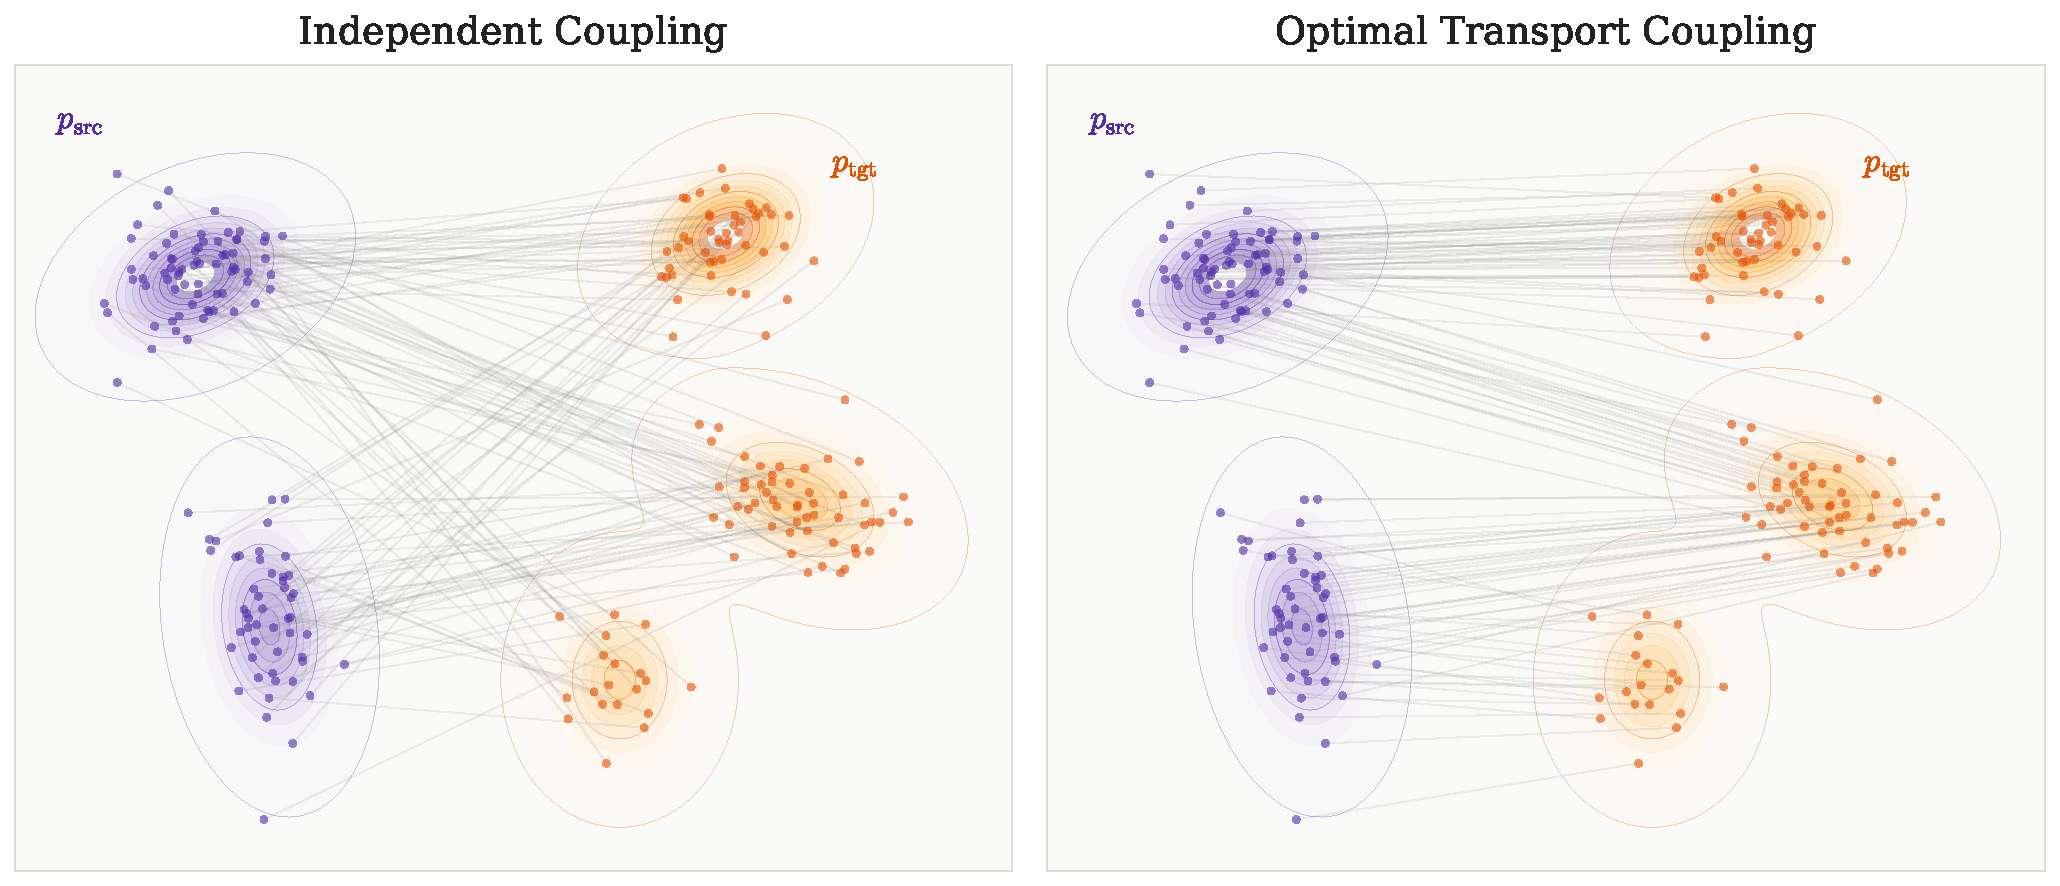
\includegraphics[width=\linewidth]{Images/PartB/ot_2d_coupling_comparison.pdf}
    \caption{\textbfs{二维中相同 $p_{\mathrm{src}}$ 和 $p_{\mathrm{tgt}}$ 之间的两种耦合。}
    左：独立（随机）配对产生交叉路径，代价较高。
    右：最优传输耦合将近处的质量配对，避免交叉。
    \figcredit{由作者在 AI 辅助编程下绘制。}}
    \label{fig:ot-2d-coupling}
\end{figure}

\paragraph{OT 问题的 Monge--Kantorovich（静态）形式。}
我们固定一个代价函数 $c:\R^D\times\R^D\to\R$，用以规定将概率质量从 $\rvx$ 发送到 $\rvy$ 的花费。目标是尽可能廉价地将源分布 $p_{\mathrm{src}}$ 变换为目标分布 $p_{\mathrm{tgt}}$。

为了定义代价，我们必须知道哪些对 $(\rvx,\rvy)$ 被匹配。这一角色由\emph{耦合}承担：它是 $\R^D\times\R^D$ 上的一个联合分布 $\gamma$，其边际分布为 $p_{\mathrm{src}}$ 和 $p_{\mathrm{tgt}}$。换言之，从 $(\rvx,\rvy)\sim\gamma$ 采样意味着我们将源中的 $\rvx$ 与目标中的 $\rvy$ 相匹配。如果 $\gamma$ 相对于勒贝格测度存在密度 $\gamma(\rvx,\rvy)$，则边际约束为
\[
\int_{\R^D} \gamma(\rvx,\rvy)\,\diff \rvy = p_{\mathrm{src}}(\rvx), 
\qquad 
\int_{\R^D} \gamma(\rvx,\rvy)\,\diff \rvx = p_{\mathrm{tgt}}(\rvy).
\]
也就是说，对 $\rvy$ 积分得到 $\rvx$ 中的源密度，而对 $\rvx$ 积分得到 $\rvy$ 中的目标密度。

我们给出两个标准示例加以说明：
\begin{enumerate}
    \item \textbfs{离散支撑。}  
    如果 $p_{\mathrm{src}}$ 和 $p_{\mathrm{tgt}}$ 支撑在有限多个点上，则一个耦合可由一个非负矩阵 $(\gamma_{ij})$ 表示，其行和等于 $p_{\mathrm{src}}(i)$，列和等于 $p_{\mathrm{tgt}}(j)$。每个元素 $\gamma_{ij}$ 是从 $i$ 发送到 $j$ 的质量数量。
    \item \textbfs{确定性映射。}  
    如果存在一个可测映射 $\rmT$ 满足 $\rmT_\#p_{\mathrm{src}}=p_{\mathrm{tgt}}$，那么
    $\gamma=(\rmI,\rmT)_\#p_{\mathrm{src}}$ 是一个确定性耦合，它将每个点
    $\rvx$ 直接移动到 $\rmT(\rvx)$。
\end{enumerate}

一旦固定了耦合 $\gamma$，传输代价就是该方案下单位代价的平均：
\[
\int c(\rvx,\rvy)\,\diff\gamma(\rvx,\rvy)
=\E_{(\rvx,\rvy)\sim\gamma}\!\big[c(\rvx,\rvy)\big].
\]
在离散情形下，它简化为 $\sum_{i,j} c_{ij}\gamma_{ij}$；在连续情形下，它变为一个二重积分。在下文中，我们将只关注连续情形。

最优传输问题即是在所有可容许耦合中，选择使该期望代价最小化的那一个。
\begin{mdframed}
\begin{equation}\label{eq:ot}
\mathrm{OT}\big(p_{\mathrm{src}},p_{\mathrm{tgt}}\big)
:= \inf_{\gamma\in\Gamma(p_{\mathrm{src}},p_{\mathrm{tgt}})}
\int c(\rvx,\rvy)\,\diff\gamma(\rvx,\rvy),
\end{equation}
\end{mdframed}
其中可行集只是施加了边际（即质量守恒）约束：
\begin{align*}
    \Gamma(p_{\mathrm{src}},p_{\mathrm{tgt}})
= \Big\{\gamma \in &\mathcal{P}(\R^D\times\R^D): \\
&\int \gamma(\rvx,\rvy) \diff \rvy = p_{\mathrm{src}}(\rvx),\,\,
\int \gamma(\rvx,\rvy)\diff \rvx = p_{\mathrm{tgt}}(\rvy)\Big\},
\end{align*}
其中 $\mathcal{P}(\R^D\times\R^D)$ 表示 $\R^D\times\R^D$ 上所有概率测度的集合。  


\subparagraph{特例：Wasserstein-2 距离。}

Wasserstein-2 距离是 Monge--Kantorovich 问题在二次代价 $c(\mathbf{x}, \mathbf{y}) = \|\mathbf{x} - \mathbf{y}\|^2$ 下的特例。它度量两个概率分布之间的距离如下：
\begin{align*}
 \mathcal{W}_2^2(p_{\mathrm{src}}, p_{\mathrm{tgt}}) := \inf_{\gamma \in \Gamma(p_{\mathrm{src}}, p_{\mathrm{tgt}})} \mathbb{E}_{(\mathbf{x}, \mathbf{y}) \sim \gamma} \left[ \|\mathbf{x} - \mathbf{y}\|^2 \right].
\end{align*}

在对 $p_{\mathrm{src}}$ 和 $p_{\mathrm{tgt}}$ 的适当假设下，Brenier 定理（见 \Cref{thm:brenier}）\footnote{Brenier 定理关于二次代价下最优传输映射的存在性与结构。特别地，如果 $p_{\mathrm{src}}$ 不赋予维数至多为 $D-1$ 的集合以质量，则最优传输映射 $\rmT^*$ 唯一存在。}保证二次代价下的最优耦合 $\gamma$ 集中于一个确定性映射 $\rmT:\mathbb{R}^D \rightarrow \mathbb{R}^D$ 的图上。因此，Wasserstein-2 距离可以等价地表示为\footnote{$\mathcal{W}_2$ 距离有三种常用形式：Monge 形式（基于最优传输映射）、Kantorovich 形式（基于耦合）以及 Benamou--Brenier 动态形式（见 \Cref{eq:bb-ot}）。在适当的正则性条件下这些形式是等价的。}：
\begin{equation}\label{eq: Monge's Formulation}    \mathcal{W}_2^2(p_{\mathrm{src}}, p_{\mathrm{tgt}}) = \inf_{\substack{\rmT:\mathbb{R}^D \rightarrow \mathbb{R}^D,\\ \text{ s.t. }\rmT\#p_{\mathrm{src}} = p_{\mathrm{tgt}}}} \mathbb{E}_{\rvx \sim p_{\mathrm{src}}} \left[ \| \rmT(\rvx) - \rvx \|^2 \right].
\end{equation}
这里 $\rmT\#p_{\mathrm{src}} = p_{\mathrm{tgt}}$ 表示 $ \rmT $ 将 $ p_{\mathrm{src}} $ 前推为 $ p_{\mathrm{tgt}} $，即当 $ \rvx \sim p_{\mathrm{src}}$ 时有 $ \rmT(\rvx) \sim p_{\mathrm{tgt}}$。 

 

因此，Wasserstein-2 距离表示在所有匹配给定边际的耦合或传输映射中，最小的期望平方传输代价。记为 $\rmT^*(\mathbf{x})$ 的最优传输映射，称为 \emph{Monge 映射}，给出了将 $p_{\mathrm{src}}$ 变换为 $p_{\mathrm{tgt}}$ 的最有效方式。

\paragraph{OT 的 Benamou--Brenier（动态）形式。} 
\begin{figure}[th!]
    \centering
    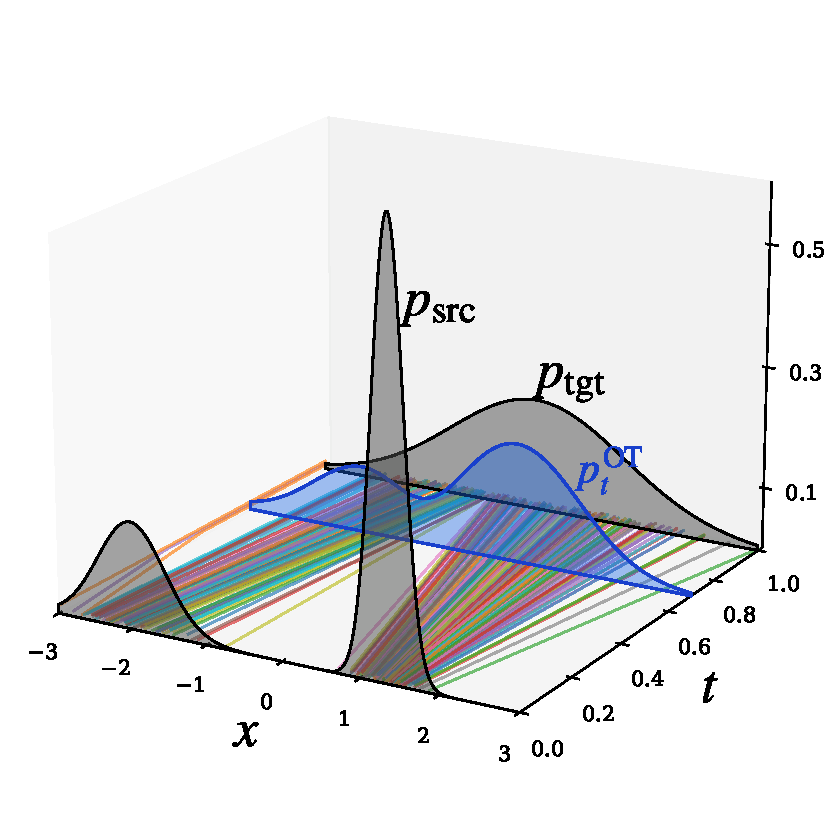
\includegraphics[width=0.8\linewidth]{Images/PartB/ot_illustration.pdf}
    \caption{ \textbfs{OT 动态视角的示意图。} 插值 $p_t^{\mathrm{OT}}$ 随时间连续演化，
提供了将 $p_{\mathrm{src}}$ 确定性地映射到 $p_{\mathrm{tgt}}$ 的最小代价传输方案（即 McCann 的位移插值）。
\figcredit{由作者绘制。}}
    \label{fig:ill-ot}
\end{figure}



不同于 Monge--Kantorovich 形式中以静态方式直接映射分布，传输也可以建模为连续时间的流：
\begin{equation*}
    p_0 := p_{\mathrm{src}} \to p_t \to p_1 := p_{\mathrm{tgt}}, \quad t \in [0,1].
\end{equation*}
这一最优传输的动态形式由 \citet{benamou2000computational} 提出，它寻求一个光滑的速度场 $ \rvv_t(\rvx) $ 来描述 $ p_t(\rvx) $ 中的质量如何随时间演化。

Benamou--Brenier 形式\footnote{Benamou–Brenier 形式描述了如何在测度与速度的连续路径上最小化动能，从而计算 $ \mathcal{W}_2 $ 距离。}表明，对于二次代价 $ c(\rvx, \rvy) = \|\rvx - \rvy\|_2^2 $（即 $ \mathcal{W}_2 $ 距离），\Cref{eq:ot} 中静态 OT 问题的最优值等于如下动能最小化问题的最优值：
%the static OT problem in \Cref{eq:ot} is equivalent \doh{``Equivalent'' is unclear.} to the following dynamic formulation:
\begin{mdframed}
   \begin{equation}\label{eq:bb-ot}
    \mathcal{W}_2^2(p_{\mathrm{src}}, p_{\mathrm{tgt}}) = \min_{\substack{ (p_t, \rvv_t) \text{ s.t. }
        \partial_t p_t + \nabla \cdot (p_t \rvv_t) = 0, \\
        p_0 = p_{\mathrm{src}},\,\, p_1 = p_{\mathrm{tgt}}
    }}
    \int_0^1 \int_{\mathbb{R}^D} \|\rvv_t(\rvx)\|^2 p_t(\rvx) \diff\rvx \diff t
\end{equation} 
\end{mdframed}
其中对每个 $t \in [0,1]$，$p_t$ 是 $\mathbb{R}^D$ 上的一个概率分布。特别地，最优传输流 $p_t(\rvx)$ 遵循 \textit{McCann 位移插值}：
\begin{equation*}
    \rmT_t^*(\rvx) = (1 - t)\rvx + t\rmT^*(\rvx),
\end{equation*}
其中 $\rmT^*(\rvx)$ 是将 $p_{\mathrm{src}}$ 传输到 $p_{\mathrm{tgt}}$ 的 OT 映射。这种线性插值使质量以常速度沿直线移动：对每个 $t \in [0,1]$ 有 $p_t = \rmT_t^*\#p_{\mathrm{src}}$。

最优传输映射 $\rmT^*$ 满足 \emph{Monge–Ampère 方程}：
%However, computing $\rmT^*$ generally requires solving the \emph{Monge–Ampère equation}:
\begin{equation}\label{eq:monge-ampere}
    p_{\mathrm{tgt}}\left(\nabla \psi(\rvx)\right) \det\left(\nabla^2 \psi(\rvx)\right) = p_{\mathrm{src}}(\rvx),
\end{equation}
其中由 Brenier 定理知，对某个凸函数 $\bpsi$ 有 $\rmT^*(\rvx) = \nabla \psi(\rvx)$。然而，这个非线性偏微分方程通常难以获得显式解。注意，这正是归一化流所使用的变量替换关系（参见 \Cref{eq:nf-change-of-var}）：流用一个具有可处理雅可比行列式的可逆传输映射进行参数化，但一般并不施加“梯度势”结构 $\rmT^*=\nabla\psi$；因此，训练得到的流可能与 Brenier/OT 映射存在显著差异。




\subsection{熵正则化最优传输（EOT）}

为了具体地引出 EOT，考虑由样本构造的经验分布。假设 $p_{\mathrm{src}}$ 支撑在点 $\{\rvx^{(i)}\}_{i=1}^n \subset \R^D$ 上且权重为 $a_i$，而 $p_{\mathrm{tgt}}$ 支撑在 $\{\rvy^{(j)}\}_{j=1}^n \subset \R^D$ 上且权重为 $b_j$。那么耦合就是一个 $n\times n$ 的非负矩阵 $\gamma=(\gamma_{ij})$，其行和匹配 $a$，列和匹配 $b$。每个元素 $\gamma_{ij}$ 表示从 $\rvx^{(i)}$ 传输到 $\rvy^{(j)}$ 的质量数量\footnote{经验（离散）测度为连续分布提供了一个有原则的代理。当地面代价为 $c(x,y)=d(x,y)^p$（从而 OT 值等于 $W_p^p$）且测度具有有限的 $p$ 阶矩时，经验测度以可量化的速率在 $W_p$ 中收敛到总体分布；参见 \citet{fournier2015rate} 以及 \citet{peyre2019computational} 中的综述。}。

\paragraph{为何要对 OT 进行正则化？}
此离散情形下的经典 OT（通过在连续形式 \Cref{eq:ot} 中取计数测度得到）归结为最小化
\[
\min_{\gamma=(\gamma_{ij})}\sum_{i,j} C_{ij}\,\gamma_{ij},
\]
约束为所有可行耦合 $\gamma=(\gamma_{ij})$，其中对于预定的地面代价 $c:\R^D\times\R^D\to\R_{\ge 0}$（例如 $c(\rvx,\rvy)=\|\rvx-\rvy\|_2^2$），$C_{ij} = c(\rvx^{(i)},\rvy^{(j)})$ 表示将一个单位质量从源点 $\rvx^{(i)}$ 移动到目标点 $\rvy^{(j)}$ 的代价。

这会产生两个主要问题：
\begin{enumerate}
    \item \textbfs{非唯一性与不稳定性：} 最小化子 $\gamma^*$ 未必唯一。例如，如果两个传输方案达到相同的最小代价，求解器可能选择其中任意一个。因此，输入 $(a,b,C)$ 的微小变化（如移动一个样本、调整权重或轻微扰动代价）都可能引起解的突变。  
    \item \textbfs{计算代价高：} 该问题是一个具有 $n^2$ 个变量和 $2n$ 个约束的线性规划。实际求解器（如匈牙利算法~\citep{kuhn1955hungarian,munkres1957algorithms}、网络单纯形法~\citep{peyre2019computational}）通常复杂度为 $\mathcal{O}(n^3)$，对大 $n$ 不可行。
\end{enumerate}

为克服这些瓶颈，EOT 目标函数在经典 OT 问题中引入了一项正则化项，由参数 $\varepsilon > 0$ 控制：
\begin{mdframed}
    \begin{align}\label{eq:eot-epsilon}
\begin{aligned}
        \text{EOT}_\varepsilon(p_{\mathrm{src}}, p_{\mathrm{tgt}}) &:= \min_{\gamma \in \Gamma(p_{\mathrm{src}}, p_{\mathrm{tgt}})} \int c(\rvx,  \rvy)  \diff\gamma(\rvx, \rvy) 
        + \varepsilon \mathcal{D}_{\text{KL}}\left(\gamma \Vert M \right).
\end{aligned}
\end{align}
\end{mdframed}
参考测度 $M$ 通常选为边际的乘积，即 $p_{\mathrm{src}} \otimes p_{\mathrm{tgt}}$。KL 散度项与传输方案 $\gamma$ 的香农熵直接相关：
\[
\mathcal{D}_{\text{KL}}(\gamma \,\Vert\, p_{\mathrm{src}} \otimes p_{\mathrm{tgt}}) = -\mathcal{H}(\gamma) + \text{Constant},
\]
其中 $\mathcal{H}(\gamma) := -\int \gamma(\rvx, \rvy) \log \gamma(\rvx, \rvy) \diff \rvx \diff \rvy$。



加入这一正则化项带来若干理论与实践上的优势，我们简要概述如下：
\paragraph{熵正则化项为何有用？}
\begin{enumerate}
  \item \textbfs{质量分散。}
  由于 $t\mapsto t\log t$ 是凸函数且对大 $t$ 增长迅速，最小化 $\int \gamma\log\gamma$
  会惩罚\emph{尖锐}耦合（某些 $\gamma(\rvx,\rvy)$ 非常大，其余接近零）。
  在总质量 $\int \gamma=1$ 固定时，它倾向于使 $\gamma(\rvx,\rvy)$ 在 $(\rvx,\rvy)\in\mathbb{R}^D\times\mathbb{R}^D$ 上分布得更均匀。
  等价地，最大化香农熵会促进更高的“不确定性”（弥散性）。

  \item \textbfs{严格凸性与唯一性。}
  由于 $\mathcal{H}$ 严格凹，\Cref{eq:eot-epsilon} 中的目标关于 $\gamma$ 严格凸，
  从而给出\emph{唯一}最小化子 $\gamma^*_\varepsilon$，且它连续依赖于 $(p_{\mathrm{src}},p_{\mathrm{tgt}},c)$。

  \item \textbfs{Sinkhorn 形式与正性。}
  在温和条件下\footnote{我们假设 $c<\infty$ 在 $p_{\mathrm{src}}\otimes p_{\mathrm{tgt}}$-几乎处处成立，并且边际核积分有限且为正。为简单起见，我们聚焦于 $\gamma^*_\varepsilon$、$p_{\mathrm{src}}$ 与 $p_{\mathrm{tgt}}$ 相对于勒贝格测度均存在密度的情形。
},
  最优解具有 \emph{Schrödinger/Sinkhorn 形式}
  \[
  \gamma^*_\varepsilon(\rvx,\rvy) = u(\rvx)\, \exp \bigl(-\tfrac{c(\rvx,\rvy)}{\varepsilon}\bigr)  \,v(\rvy)p_{\mathrm{src}}(\rvx) p_{\mathrm{tgt}}(\rvy),
  \]
  其中 $u,v$ 为正的缩放函数（在相差一个全局常数因子下唯一）。实践中，连续形式用有限样本近似，从而将 EOT 归约为有限（采样的）Sinkhorn 迭代。
该熵正则化目标严格凸，缩放（Sinkhorn/IPFP）算法可高效求解~\citep{sinkhorn1964relationship,cuturi2013sinkhorn}。
对于每个边际有 $n$ 个支撑点（即 $n\times n$ 核）的稠密问题，每次 Sinkhorn 迭代的时间与内存均为 $\mathcal{O}(n^2)$，
使该方法更具可扩展性和实用性~\citep{altschuler2017near}。

  \item \textbfs{$\varepsilon$ 的极限。}
当 $\varepsilon \to 0$ 时，最优方案 $\gamma^*_\varepsilon$ 越来越集中，逼近（可能奇异的）经典 OT 耦合（我们将在 \Cref{subsec:eot-ot} 中重新审视这一联系）。
当 $\varepsilon$ 增大时，$\gamma^*_\varepsilon$ 逐渐铺展开来，并逼近独立耦合 $p_{\mathrm{src}}\otimes p_{\mathrm{tgt}}$。
\end{enumerate}



\subsection{薛定谔桥（SB）}\label{subsec:sb}


\paragraph{SB 的 KL 形式。}
薛定谔桥（SB）问题由 Erwin Schrödinger 于 20 世纪 30 年代提出，它提出如下问题。假设粒子按某种简单的参考动力学（例如布朗运动）运动。现在设想我们在两个时刻观测粒子：在 $t=0$ 时其分布为 $p_{\mathrm{src}}$，在 $t=1$ 时为 $p_{\mathrm{tgt}}$。在所有连接这两个分布的随机过程中，哪一个偏离参考动力学最小？这里“偏离”由 KL 散度度量，因此 SB 问题的解是将布朗运动变形为满足预定边界条件的过程的最可能方式。

为使其精确化，令 $\rvx_{0:T}:=\{\rvx_t\}_{t\in[0,T]}$ 表示过程的一条完整轨迹。我们用 $P$ 表示\emph{轨迹的律}（law），即整个样本路径上的概率分布。$P$ 的时间 $t$ 边际记为 $p_t$（或 $P_t$），它描述单个时刻状态 $\rvx_t$ 的分布。形式上，对于可测集 $A\subseteq\mathbb R^D$，
\[
p_t(A) = P(\rvx_t \in A).
\]
换言之，$p_t$ 可视为如下的经验分布：从 $P$ 中采样许多条完整轨迹，然后收集 $t$ 时刻的状态——例如，当状态为一维时表现为直方图。


考虑一个由如下 SDE 驱动的参考扩散 $\{\rvx_t\}_{t\in[0,T]}$
\begin{align}\label{eq:general-sb-sde}
    \diff \rvx_t  =  \rvf(\rvx_t,t)\,\diff t  +  g(t)\,\diff \rvw_t,
\end{align}
其中 $\rvf\colon \R^D\times[0,T]\!\to\!\R^D$，$g\colon[0,T]\!\to\!\R$，且
$\{\rvw_t\}_{t\in[0,T]}$ 是标准布朗运动。  
记 $R$ 为完整轨迹
$\rvx_{0:T}:=\{\rvx_t\}_{t\in[0,T]}$ 的\emph{路径律}（联合分布）；这个 $R$ 将作为\emph{参考}轨迹分布。

采用上述记号，SB 问题寻求一个轨迹律 $P$，使其在 KL 散度下最接近 $R$，同时匹配预定的端点边际：
\begin{align}\label{eq:sb-epsilon-general}
    \mathrm{SB}(p_{\mathrm{src}}, p_{\mathrm{tgt}})
    := \min_{P}\, \mathcal{D}_{\mathrm{KL}}(P\|R)
    \quad \text{s.t.} \quad P_0 = p_{\mathrm{src}},\;\; P_T = p_{\mathrm{tgt}}.
\end{align}
最优解 $P^*$ 依赖于所选的参考过程 $R$。

\paragraph{SB 的随机控制视角。}

\begin{figure}[th!]
    \centering
    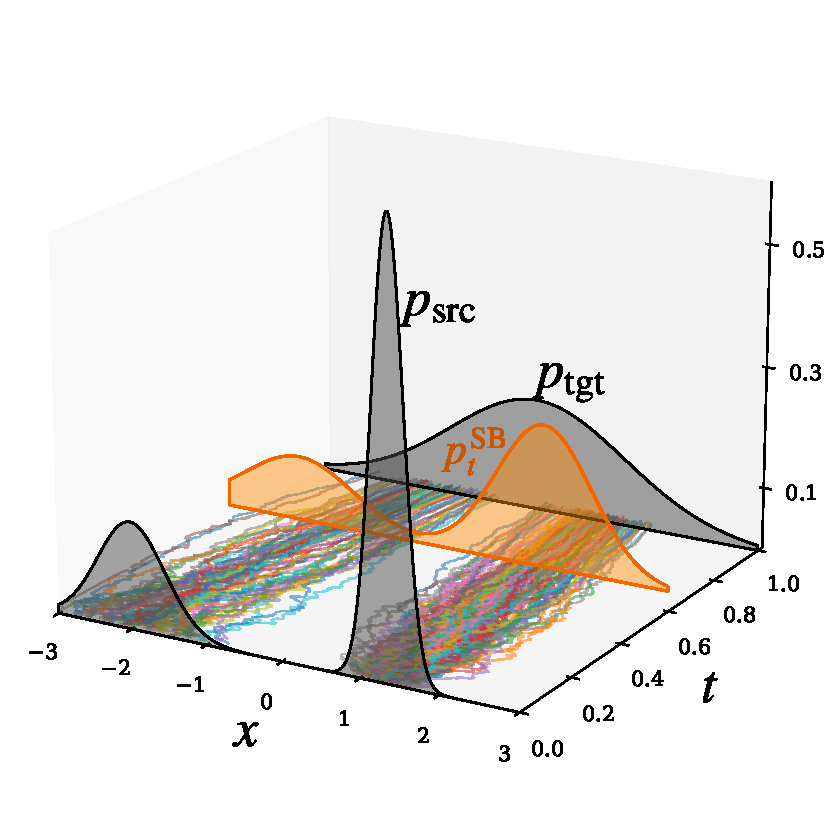
\includegraphics[width=0.8\linewidth]{Images/PartB/sb_illustration.pdf}
    \caption{\textbfs{SB 的随机控制视角示意图。} 该桥寻求在连接 $p_{\mathrm{src}}$ 与 $p_{\mathrm{tgt}}$ 的同时偏离参考最少的随机路径。
    \figcredit{由作者绘制。}}
    \label{fig:ill-sb}
\end{figure}


与其在 \Cref{eq:sb-epsilon-general} 中对任意路径分布 $P$ 进行优化，一种更易处理的途径是将参考动力学作为锚点并允许其漂移。这通过引入一个随时间变化的漂移 $\rvv_t(\rvx_t)$ 来实现，它扰动参考过程并生成一族候选轨迹分布。所得动力学具有\emph{受控扩散}的形式：
\[
    \diff \rvx_t
    = \bigl[\rvf(\rvx_t,t) + \rvv_t(\rvx_t)\bigr]\diff t + g(t) \diff \rvw_t,
\]
其中 $\rvv_t:\R^D\to\R^D$ 是待后优化的漂移（\Cref{eq:sb-kinetic}）。 在标准的可积性条件（如 Novikov 条件）下，并由 Girsanov 定理
（见 \Cref{subsec:girsanov}），受控律 $P$ 与参考 $R$ 之间的 KL 散度具有动态（动能）形式
\begin{align*}
    \mathcal{D}_{\mathrm{KL}}(P\|R)
    = \E_{P}\!\left[\frac{1}{2}\int_0^T \frac{\|\rvv_t(\rvx_t)\|^2}{g^2(t)} \diff t\right]
    = \frac{1}{2}\int_0^T\!\int_{\R^D}\frac{\|\rvv_t(\rvx)\|^2}{g^2(t)} p_t(\rvx) \diff \rvx \diff t,
\end{align*}
其中 $p_t$ 是受控过程下 $\rvx_t$ 的时间 $t$ 边际。第二个等式由全期望公式得到。

因此，SB 问题可重新表述为：在所有将过程从 $t=0$ 处的 $p_{\mathrm{src}}$ 驾驭到 $t=T$ 处 $p_{\mathrm{tgt}}$ 的可容许漂移 $\rvv_t$ 上，最小化期望控制能量
\citep{dai1991stochastic,pra1990markov,pavon1991free,chen2016relation}。这导出\emph{随机控制形式}：
\begin{mdframed} 
\begin{align}\label{eq:sb-kinetic} 
\begin{aligned} &\mathrm{SB}_\varepsilon(p_{\mathrm{src}}, p_{\mathrm{tgt}}) \\= & \min_{\substack{ \mathbf{v}_t \text{ s.t. } \diff \rvx_t = \left[\rvf(\rvx_t, t) + \mathbf{v}_t(\rvx_t) \right]\diff t + g(t) \diff \rvw_t, \\ \rvx_0 \sim p_{\mathrm{src}}, \,\, \rvx_T \sim p_{\mathrm{tgt}} }} \frac{1}{2} \int_0^T\int_{\mathbb{R}^D} \frac{\norm{\rvv_t(\rvx)}^2}{g^2(t)} p_t(\rvx)\diff \rvx \diff t, 
\end{aligned}
\end{align} 
\end{mdframed}

重要的是，端点分布 $p_{\mathrm{src}}$ 和 $p_{\mathrm{tgt}}$ 是任意的；
控制 $\rvv_t$ 的选择正是为了在这些边际之间“桥接”参考动力学，同时尽可能（在 KL 散度下）接近参考过程 $R$。

\paragraph{特殊的布朗参考。}
\Cref{eq:sb-kinetic} 类似于 \Cref{eq:bb-ot} 中 OT 的 Benamou--Brenier 形式，尤其当参考过程 $R^\varepsilon$（$\varepsilon>0$）选为布朗
运动\footnote{这种相似性可以严格化。在一种等价的时间对称流体动力学形式中，若 $\tilde{\rvv}_t$ 表示满足连续性方程
$\partial_t \rho_t + \nabla \cdot (\rho_t \tilde{\rvv}_t)=0$ 的当前速度，则布朗参考 SB 目标（\Cref{eq:sb-epsilon-kinetic}）可
写为 Benamou--Brenier 型动能项（至多差一个约定常数因子）加上一个 Fisher 信息项：
\[
\int_0^T\!\!\int
\left[
\frac{1}{2}\|\tilde{\rvv}_t(\rvx)\|^2
+
\frac{\varepsilon^2}{8}\|\nabla_{\rvx}\log \rho_t(\rvx)\|^2
\right]\rho_t(\rvx)\,\diff\rvx\,\diff t.
\]
因此，在布朗参考 / 二次代价情形下，熵正则化最优传输可视为动态 OT 的 Fisher 信息正则化版本；参见
\citet{chen2021stochastic} 中的问题 4.6。}：
\[
\diff \rvx_t = \sqrt{\varepsilon}\,\diff\rvw_t,
\]
从而 $\rvf \equiv \mathbf{0}$ 且 $g(t) \equiv \sqrt{\varepsilon}$。

在此设定下，SB 问题寻求一个在 KL 散度下最接近布朗参考 $R^\varepsilon$ 的路径分布 $P$，同时匹配端点边际：
\begin{align}\label{eq:sb-epsilon}
    \mathrm{SB}_\varepsilon(p_{\mathrm{src}}, p_{\mathrm{tgt}})
    := \min_{P} \mathcal{D}_{\mathrm{KL}}(P \| R^\varepsilon)
    \quad \text{s.t.} \quad P_0 = p_{\mathrm{src}}, \;\; P_T = p_{\mathrm{tgt}}.
\end{align}
等价的随机控制形式则变为
\begin{align}\label{eq:sb-epsilon-kinetic}
\begin{aligned}
    \mathrm{SB}_\varepsilon(p_{\mathrm{src}}, p_{\mathrm{tgt}})
    = \min_{\substack{
        \rvv_t \text{ s.t. } \diff \rvx_t = \rvv_t(\rvx_t)\,\diff t + \sqrt{\varepsilon}\,\diff \rvw_t, \\
        \rvx_0 \sim p_{\mathrm{src}},\;\; \rvx_T \sim p_{\mathrm{tgt}}
    }}
    \frac{1}{2\varepsilon}\int_0^T \!\!\int_{\R^D}
        \|\rvv_t(\rvx)\|^2 \, p_t(\rvx)\,\diff \rvx\,\diff t,
\end{aligned}
\end{align}
其中 $p_t$ 表示由漂移 $\rvv_t$ 驱动的扩散的时间 $t$ 边际：
\[
\diff \rvx_t = \rvv_t(\rvx_t)\,\diff t + \sqrt{\varepsilon}\,\diff \rvw_t.
\]



\paragraph{为何需要指定参考分布？} 
与经典 OT 不同，SB 问题由于其随机性而需要一个参考分布。在 OT 中，代价函数（例如 $c(\rvx, \rvy) \propto \|\rvx - \rvy\|^2$）隐式地定义了唯一的确定性测地线路径，使参考变得不必要。相反，SB 设定允许无穷多个连接边际的随机过程，且没有内在的“自然”路径概念。参考测度 $R$ 编码了系统潜在的物理或几何结构（例如布朗运动），并定义了基于 KL 的优化目标 $\mathcal{D}_{\mathrm{KL}}(P \| R)$，否则最优性的概念便无法定义。



\paragraph{耦合 PDE 刻画。}  
描述 SB 解的一种便捷方式是借助两个时空势 $\Psi(x,t)$ 和 $\widehat{\Psi}(x,t)$。令
$p_t^{\mathrm{SB}}$ 表示 \Cref{eq:sb-epsilon-general} 中最优轨迹律 $P^*$ 在时间 $t\in[0,T]$ 处的边际。则有如下对称分解~\citep{dai1991stochastic}
\begin{align}\label{eq:sb-symmetry}
p_t^{\mathrm{SB}}(x) = \Psi(x,t) \widehat{\Psi}(x,t),
\end{align}
其中 $\Psi$ 和 $\widehat{\Psi}$ 求解（线性的）\emph{Schrödinger 方程组}~\citep{caluya2021wasserstein,chen2021stochastic,chenlikelihood}：
\begin{align}
\begin{aligned}\label{eq:pde-schrodinger}
\frac{\partial \Psi}{\partial t}(\mathbf{x},t)
  &= -\nabla_{\mathbf{x}} \Psi(\mathbf{x},t) \cdot \rvf(\mathbf{x},t)
     - \frac{g^2(t)}{2}\,\Delta_\mathbf{x} \Psi(\mathbf{x},t),  \\
\frac{\partial \widehat{\Psi}}{\partial t}(\mathbf{x},t)
  &= -\nabla_{\mathbf{x}}\!\cdot\!\bigl(\widehat{\Psi}(\mathbf{x},t)\,\rvf(\mathbf{x},t)\bigr)
     + \frac{g^2(t)}{2}\,\Delta_\mathbf{x}\widehat{\Psi}(\mathbf{x},t) 
\\[4pt] \text{subject to}  \\[4pt]
\Psi(\mathbf{x},0)&\,\widehat{\Psi}(\mathbf{x},0) = p_{\mathrm{src}}(\mathbf{x}),
\quad
\Psi(\mathbf{x},T)\,\widehat{\Psi}(\mathbf{x},T) = p_{\mathrm{tgt}}(\mathbf{x}). 
\end{aligned}
\end{align}

\iffalse

\begin{align}
\begin{aligned}\label{eq:pde-schrodinger}
\frac{\partial \Psi}{\partial t}(\mathbf{x},t)
  &= -\nabla_{\mathbf{x}} \Psi(\mathbf{x},t)^\top\,\rvf(\mathbf{x},t)
     - \frac{1}{2}\,\mathrm{Tr}\bigl(g^2(t)\,\nabla_{\mathbf{x}}^2\Psi(\mathbf{x},t)\bigr),  \\
\frac{\partial \widehat{\Psi}}{\partial t}(\mathbf{x},t)
  &= -\nabla_{\mathbf{x}}\!\cdot\!\bigl(\widehat{\Psi}(\mathbf{x},t) \rvf(\mathbf{x},t)\bigr)
     + \frac{1}{2} \mathrm{Tr}\bigl(g^2(t)\,\nabla_{\mathbf{x}}^2\widehat{\Psi}(\mathbf{x},t)\bigr) 
\\[4pt] \text{subject to}  \\[4pt]
\Psi(\mathbf{x},0)& \widehat{\Psi}(\mathbf{x},0) = p_{\mathrm{src}}(\mathbf{x}),
\quad
\Psi(\mathbf{x},T) \widehat{\Psi}(\mathbf{x},T) = p_{\mathrm{tgt}}(\mathbf{x}). 
\end{aligned}
\end{align}
\fi

\subparagraph{正向时间的薛定谔桥 SDE。}
一旦已知 $\Psi$，最优动力学即是被时空因子 $\Psi$ 倾斜后的参考扩散：
\begin{align}\label{eq:sb-forward-sde}
    \diff \rvx_t = \bigl[\rvf(\rvx_t, t) + g^2(t)\,\nabla_{\mathbf{x}} \log \Psi(\rvx_t, t)\bigr]\diff t
+ g(t)\diff \rvw_t, \quad \rvx_0 \sim p_{\mathrm{src}}.
\end{align}
令 $Q$ 表示 \Cref{eq:sb-forward-sde} 的轨迹律
（故由 \Cref{eq:sb-symmetry,eq:pde-schrodinger} 知 $Q_0=p_{\mathrm{src}}$ 且 $Q_T=p_{\mathrm{tgt}}$）。则
\emph{$Q=P^*$} 且 \Cref{eq:sb-kinetic} 的最小化子 $\rvv^*$ 为（见 \citep{chen2021stochastic} 的第 4.6 节）： 
\[
\rvv_t^{*}(\rvx) = g^2(t) \nabla_\rvx \log \Psi(\rvx,t).
\]
也就是说，
漂移校正 $g^2\nabla_\rvx\log\Psi$ 恰好是为匹配端点边际而对参考施加的
最小 KL 扰动。

%\textcolor{red}{In other words, the optimal control $\mathbf{v}_t(\rvx_t)$ of the stochastic control formulation \Cref{eq:sb-kinetic} of SB is given by
%\begin{align*}
%    \mathbf{v}_t(\rvx_t) = \rvf(\rvx_t, t) + g^2(t)\,\nabla_{\mathbf{x}} \log \Psi(\rvx_t, t).
%\end{align*}
%}

\subparagraph{逆向时间的薛定谔桥 SDE。}
同一个最优路径律也可以在时间上逆向生成。考察逆向时间漂移形式的一种便捷方式是，在概念上使用扩散的标准时间反演恒等式：
\[
\rvb^{-}(\rvx,t)=\rvb^{+}(\rvx,t)-g^2(t)\nabla_\rvx\log p_t^{\mathrm{SB}}(\rvx),
\]
其中 $\rvb^{+}=\rvf+g^2\nabla\log\Psi$ 且 $p_t=\Psi\,\widehat{\Psi}$。这给出
\[
\rvb^{-}(\rvx,t)=\rvf(\rvx,t)-g^2(t) \nabla_\rvx\log \widehat{\Psi}(\rvx,t).
\]
于是逆向时间 SDE 为
\begin{align}\label{eq:sb-backward-sde}
\diff \rvx_t
= \Big[\rvf(\rvx_t,t) - g^2(t) \nabla_{\rvx}\log \widehat{\Psi}(\rvx_t,t)\Big]\diff t
+ g(t)\,\diff \bar{\rvw}_t, \quad \rvx_T \sim p_{\mathrm{tgt}} .
\end{align}
等价地，通过 $\rvy_\tau := \rvx_{T-\tau}$ 重新参数化时间，使
$\tau$ 从 $0$ 增加到 $T$。则 $\rvy_\tau$ 在 $\tau$ 上正向演化，从 $\rvy_0 \sim p_{\mathrm{tgt}}$ 出发，演化为
\begin{align}\label{eq:sb-reverse-forward-tau}
\begin{aligned}
    \diff \rvy_\tau
= \big[-\rvf(\rvy_\tau,T-\tau) + g^2(T-\tau) \nabla_{\rvy}\log \widehat{\Psi}(\rvy_\tau,&T-\tau)\big]\diff \tau
\\&+ g(T-\tau) \diff \rvw_\tau.
\end{aligned}
\end{align}
在 \Cref{eq:sb-kinetic} 的逆向时间随机控制形式中（采用相同的二次能量，但时钟反转）：
\begin{align}
\min_{\substack{
\rvu_\tau \text{ s.t. }  
\diff \rvy_\tau = \left[-\rvf(\rvy_\tau,T-\tau)+\rvu_\tau(\rvy_\tau)\right]\diff\tau
+ g(T-\tau) \diff \rvw_\tau,\\
\rvy_0 \sim p_{\mathrm{tgt}},\ \rvy_T \sim p_{\mathrm{src}}
}}
\tfrac12 \int_{0}^{T} \int_{\R^D} \tfrac{\|\rvu_\tau(\rvy)\|^2}{g^2(T-\tau)}\,p_{T-\tau}(\rvy)  \diff\rvy \diff\tau .
\end{align}
最优控制为
\[
\rvu_\tau^{*}(\rvy)=g^2(T-\tau)\nabla_{\rvy}\log\widehat{\Psi}(\rvy,T-\tau).
\]



正向与逆向描述都给出相同的最优路径律 $P^*$，二者由如下关系联系
\[
\nabla\log p_t^{\mathrm{SB}}=\nabla\log\Psi+\nabla\log\widehat\Psi,
\qquad
\rvb^{-}=\rvb^{+}-g^2\,\nabla\log p_t^{\mathrm{SB}},
\]
因此它们的边际在每个时刻都与 $p_t^{\mathrm{SB}}$ 一致。  附加漂移项 $g^2\nabla\log\Psi$（正向）和
$-\,g^2\nabla\log\widehat{\Psi}$（逆向）充当控制力，在保持与参考的相对熵最接近的同时，
驾驭参考扩散以匹配端点边际。




\subparagraph{耦合 PDE 方法的实际障碍。}
为了基于 \Cref{eq:sb-backward-sde} 构造生成过程，必须求解 \Cref{eq:pde-schrodinger} 中的耦合 PDE 以获得逆向薛定谔势 $\widehat{\Psi}$。然而，这些 PDE 即使在低维设定下也以难解著称，这使得它们在生成建模中的直接应用充满挑战。为绕开这一困难，已有若干工作提出了替代策略：利用 Score SDE 技术迭代地求解每个半桥问题（$p_{\mathrm{tgt}} \leftarrow p_{\mathrm{src}}$ 和 $p_{\mathrm{tgt}} \rightarrow p_{\mathrm{src}}$）~\citep{de2021diffusion}；优化代理似然界~\citep{chenlikelihood, liu20232}；或基于样本对 $(\rvx_0, \rvx_T) \sim p_{\mathrm{src}} \otimes p_{\mathrm{tgt}}$ 的后验 $\rvx_t \vert \rvx_0, \rvx_T$ 的解析解设计免仿真训练~\citep{liu20232}。我们在此不深入技术细节，而是在 \Cref{sec:dm-and-sb} 中简要讨论扩散模型与 SB 之间的联系。

\subsection{全局前推与局部动力学：DGM 的 OT 类比}
从最优传输视角（\Cref{eq:ot}）出发，可以利用深度生成模型学习一个从简单先验到数据的传输（前推）映射，即 
$\rmG_{\bm{\phi}\#}p_{\mathrm{prior}} \approx p_{\mathrm{data}}$。 
尽管 $\rmG_{\bm{\phi}}$ 一般并不与最优传输映射重合
（除了在适当条件下施加 OT 目标的工作~\citep{genevay2018learning,onken2021ot}），
Benamou--Brenier 形式（\Cref{eq:bb-ot}）提供了一个互补的动态视角。
它不是直接学习单个全局映射，而是将传输描述为由随时间变化的局部向量场生成的连续流，在 $p_{\mathrm{prior}}$ 与 $p_{\mathrm{data}}$ 之间描绘出一条光滑路径。
这一动态形式与静态薛定谔桥问题（\Cref{eq:sb-epsilon-general}）及其随机控制对应物（\Cref{eq:sb-kinetic}）之间的关系相平行，
其中最优耦合实现为一个受控扩散过程。
生成建模中也出现了类似的类比：
诸如 GAN 或 VAE 的标准 DGM 学习一个全局前推映射，
而扩散模型学习一个驱动生成动力学的、随时间变化的局部向量场。




\newpage
\section{不同最优传输形式之间的关系}\label{sec:relation-ot}

\begin{figure}[ht!]
\centering
%In EOT and OT, the cost function is typically quadratic: $c(\rvx, \rvy)\propto\norm{\rvx-\rvy}_2^2$.}
\resizebox{\textwidth}{!}{% <-- REMOVED
\begin{tikzpicture}[
    node distance=2.2cm and 1.2cm,  % <-- REDUCED spacing
    block/.style={
        rectangle, draw, thick, rounded corners,
        fill=white!10, text width=13em,   % <-- REDUCED text width
        minimum height=5em, align=center, font=\normalsize % <-- CHANGED font to normalsize
    },
    arrow/.style = {ultra thick, -{Stealth[length=4mm, width=4mm]}},
    dashed_arrow/.style={-Latex, ultra thick, dashed, color=gray, -{Stealth[length=4mm, width=4mm]}},
    label/.style={midway, font=\small, align=center}
]

% Nodes
\node[block, text width=11em] (sde) {
    {\large \textbfs{SB}$_\varepsilon$ \\ \textbfs{（随机控制）}}\\[0.6em] 
见 \Cref{eq:sb-epsilon-kinetic}。
};

\node[block, text width=11em, below=of sde] (ode) {
   {\large \textbfs{OT} \\ \textbfs{（动态形式）}
   \\ [0.5em]
见 \Cref{eq:bb-ot}。
   }
};

\node[block, text width=11em, right=of sde, xshift=1.5cm] (sb) {
    {\large \textbfs{SB}$_\varepsilon$ \\ \textbfs{（静态形式）}}\\[0.5em]
$\displaystyle
\min_{\substack{P :\, P_0 = p_{\rm src} \\ \phantom{P :\, } P_T = p_{\rm tgt}}}
  \mathcal{D}_\mathrm{KL}(P \| R^\varepsilon)
$
};

\node[block, right=of sb, xshift=1.5cm] (eot) {
    {\large \textbfs{EOT}$_\varepsilon$ }\\[0.5em]
    $\displaystyle
        \min_{\gamma \in \Gamma(p_{\rm src}, p_{\rm tgt})}
        \int \norm{\rvx-\rvy}_2^2  \diff\gamma
         + \varepsilon  \mathcal{D}_{\mathrm{KL}}(\gamma \| p_{\rm src} \otimes p_{\rm tgt})
    $

};

\node[block, below=of eot] (ot) {
 {\large \textbfs{OT \\ （静态形式）} }\\[0.6em]
    $\displaystyle
        \min_{\gamma \in \Gamma(p_{\rm src}, p_{\rm tgt})}
        \int \norm{\rvx-\rvy}_2^2 \diff\gamma
    $
};

% Arrows using the new 'label' style
\draw[arrow] (sde) -- (ode)
    node[label, left]
    {$\varepsilon \to 0$}
    node[label, right]
    {(iv)};
\draw[arrow,<->] (sde.east) -- (sb.west)
  node[pos=.5, above, text width=9em, align=center, sloped]
    {\footnotesize$p_t = P^*(\rvx_t \in \cdot)$}
  node[pos=.5, below, text width=9em, align=center, sloped]{(i)};
\draw[arrow,<->] (sb.east) -- (eot.west)
  node[pos=.5, above, text width=8em, align=center, sloped]
    {端点投影\\ \footnotesize$\gamma^* = (\rvx_0,\rvx_T)_\# P^*$}
  node[pos=.5, below, text width=9em, align=center, sloped]
    {(ii)};
\draw[arrow] (eot) -- (ot)
    node[label, left]
    {$\varepsilon \to 0$}
    node[label, right]
    {(iii)};
\draw[arrow, <->] (ode) -- ([yshift=0.3cm] ot.west)
    node[label, below]
    {$p_t = \bPsi_t\#\gamma^*$ 其中 $\bPsi_t(\rvx,\rvy) = (1-t) \rvx + t \rvy$};
    
\end{tikzpicture}
}
\caption{\textbfs{最优传输各变体之间的关系，其中 $c(\rvx,\rvy)=\|\rvx-\rvy\|_2^2$，SB 中的参考为 $R^\varepsilon$。}
我们总结如下等价关系：(i) $\mathrm{SB}_\varepsilon$（随机控制）$\Leftrightarrow$ $\mathrm{SB}_\varepsilon$（静态形式），其中 $p_t$ 是路径测度 $P$ 的时间 $t$ 边际；(ii) $\mathrm{SB}_\varepsilon$（静态形式）$\Leftrightarrow$ $\mathrm{EOT}_\varepsilon$（见 \Cref{subsec:sb-eot}）；(iii) $\mathrm{EOT}_\varepsilon$（静态形式）$\Leftrightarrow$ $\mathrm{OT}_\varepsilon$（静态）（见 \Cref{subsec:eot-ot}）；(iv) $\mathrm{SB}_\varepsilon$（随机控制）$\Leftrightarrow$ $\mathrm{OT}$（动态）（见 \Cref{subsec:sb-ot}）。\Cref{fig:eot-epsilon} 同时可视化了联系~(iii) 和~(iv)：
随着 $\varepsilon$ 减小，耦合与传输路径都从随机 SB 区域收敛到确定性 OT。
\figcredit{由作者绘制。}} 
\label{fig:ot-dm}
\end{figure}


在深入技术细节之前，先澄清最优传输及其熵正则化的不同形式之间如何联系会很有帮助。在高层次上，这些问题可以视为相互关联的（其关联图见 \Cref{fig:ot-dm}）：
\begin{enumerate}
    \item[(i)]  以布朗运动给定的特定参考 $R^\varepsilon$ 的 SB 问题 $\mathrm{SB}_\varepsilon$
\[
\diff \rvx_t = \sqrt{\varepsilon}\,\diff \rvw_t
\]
等价于其静态形式：演化的边际 $p_t$ 恰好是最优路径测度 $P$ 的时间 $t$ 切片（见 \Cref{subsec:sb}）；
    \item[(ii)] $\mathrm{SB}_\varepsilon$ 的静态形式直接联系到熵正则化最优传输问题 $\mathrm{EOT}_\varepsilon$（见 \Cref{subsec:sb-eot}）；
    \item[(iii)] $\mathrm{EOT}_\varepsilon$ 反过来可以关联到熵正则化最优传输的静态形式 $\mathrm{OT}_\varepsilon$（见 \Cref{subsec:eot-ot}）；
    \item[(iv)] $\mathrm{SB}_\varepsilon$ 的随机控制视角也可以联系到经典 OT 的动态形式（见 \Cref{subsec:sb-ot}）。  
\end{enumerate}


这些非平凡的关系共同提供了一个跨越随机控制、熵正则化以及经典 OT 框架的紧凑视角。




\begin{figure}[th!]
    \centering
    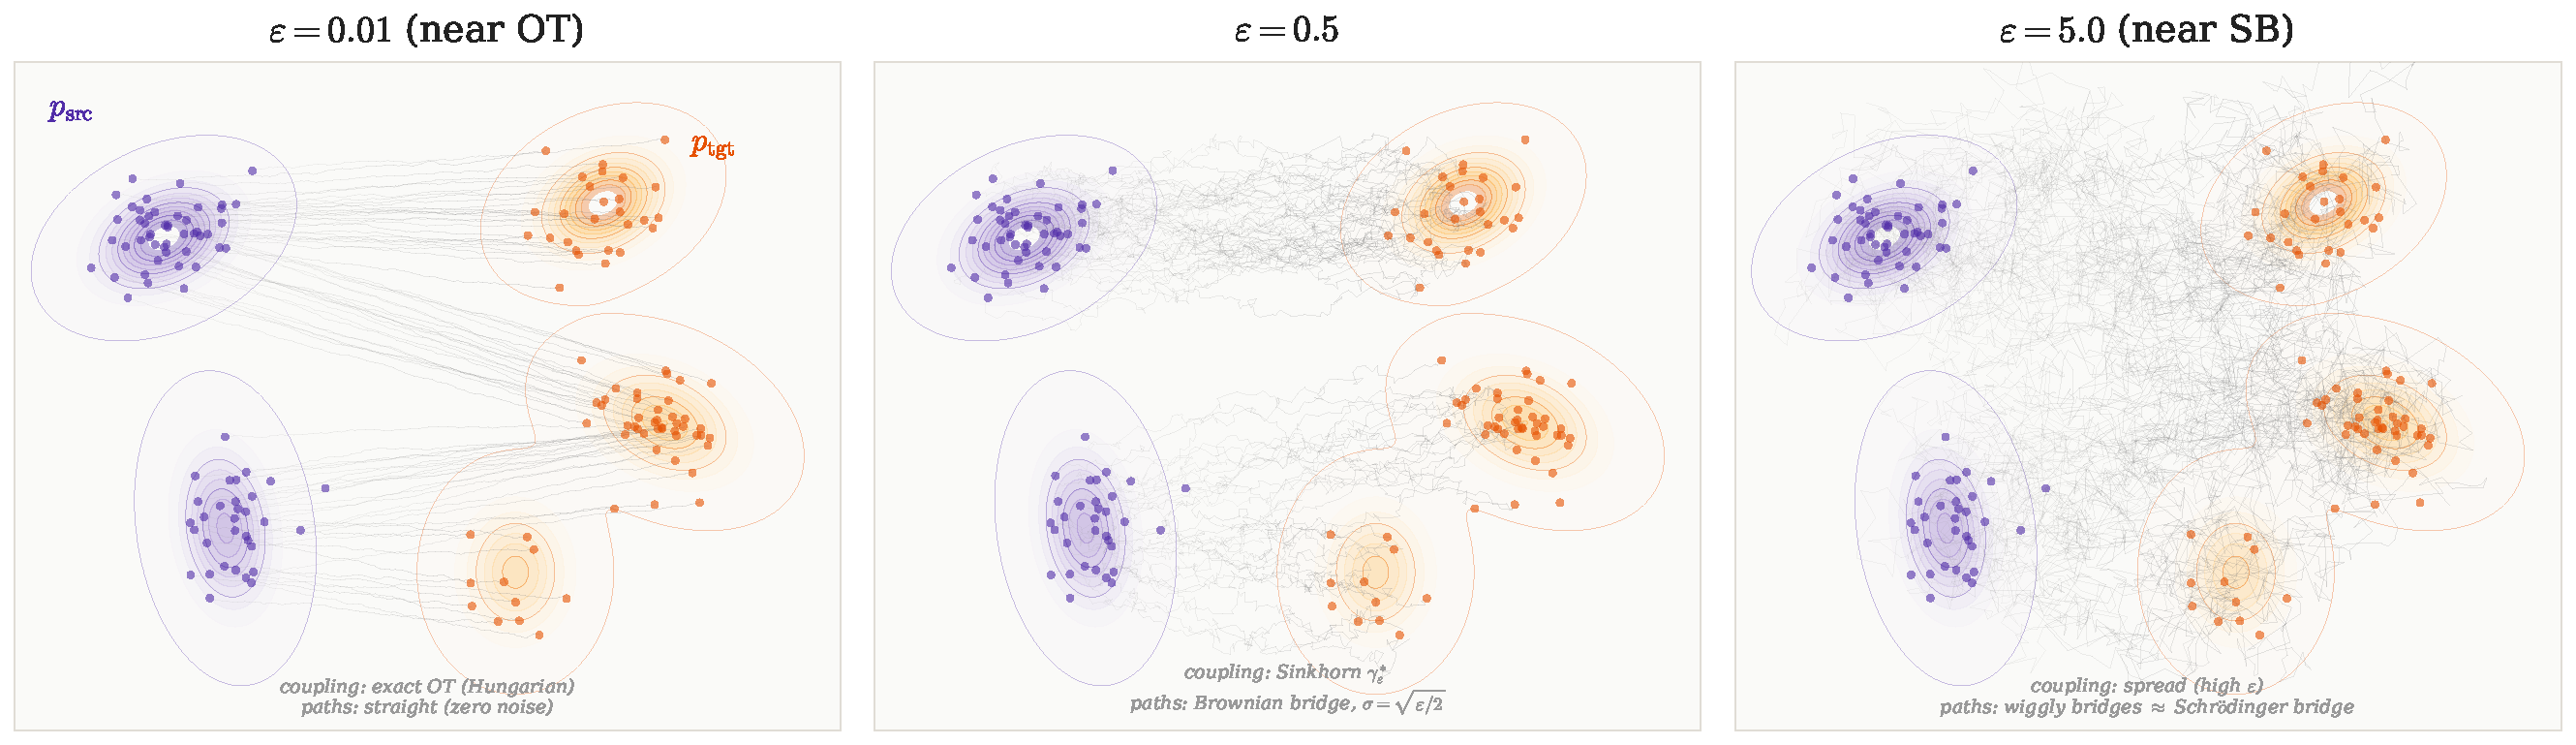
\includegraphics[width=\linewidth]{Images/PartB/eot_epsilon_interpolation.pdf}
    \caption{\textbfs{正则化参数 $\varepsilon$ 对熵正则化最优传输的影响（联系 (iii) 和 (iv)）。}
    随着 $\varepsilon$ 增大，两件事同时发生：
    耦合 $\gamma^*_\varepsilon$ 将质量铺展到更远的目标，
    传输路径也变得越来越随机。
    左（$\varepsilon=0.01$）：路径几乎为直线，每个源点映射到单一邻近目标，恢复经典 OT。
    中（$\varepsilon=0.5$）：路径出现可见波动，耦合开始铺展。
    右（$\varepsilon=2.5$）：路径高度随机，
    逼近薛定谔桥区域；
    在极限 $\varepsilon\to\infty$ 下，耦合退化为
    独立乘积 $p_{\mathrm{src}}\otimes p_{\mathrm{tgt}}$。
    耦合通过 Sinkhorn 算法计算
    （$\varepsilon\to 0$ 时用匈牙利算法）；
    在端点给定的条件下，路径是布朗桥，
    扩散系数 $\sigma=\sqrt{\varepsilon/2}$，
    来自 Mikami 对偶（\Cref{subsec:sb-eot}）。
    \figcredit{由作者在 AI 辅助编程下绘制。}}
    \label{fig:eot-epsilon}
\end{figure}

\subsection{SB 与 EOT 是（对偶）等价的}\label{subsec:sb-eot}
在本节中，我们给出两个互补的视角，表明 SB 本质上等价于 EOT。  
与产生单一确定性映射的经典最优传输不同，SB 产生粒子的\emph{随机}流：质量以概率方式被传输，边际在类扩散动力学下演化。

从静态视角看，SB 与 EOT 一致，其目标是找到两个端点分布之间的耦合，在传输代价与熵之间取得平衡。  
从动态视角看，SB 描述一个受控扩散过程，在仍匹配所需端点的同时，尽可能接近一个简单参考（如布朗运动）。  每个视角都独立地确立了这一等价性，为理解 SB/EOT 作为分布到分布变换的典型形式化提供了两种一致的方式。



\paragraph{静态薛定谔桥。}
令
\[
  \widetilde R^\varepsilon(\rvx,\rvy)
  := \frac{1}{Z_\varepsilon}\,e^{-c(\rvx,\rvy)/\varepsilon}\,p_{\mathrm{src}}(\rvx)\,p_{\mathrm{tgt}}(\rvy),
\]
其中归一化常数为
\[
Z_\varepsilon := \iint e^{-c(\rvx, \rvy)/\varepsilon}\, p_{\mathrm{src}}(\rvx)\, p_{\mathrm{tgt}}(\rvy)\,\mathrm d\rvx\,\mathrm d\rvy.
\]
则对任意可容许耦合 \(\gamma\in\Gamma(p_{\mathrm{src}},p_{\mathrm{tgt}})\)，直接计算给出
\[
\int c\, \mathrm d\gamma
+\varepsilon \mathcal{D}_\mathrm{KL}\!\bigl(\gamma \Vert p_{\mathrm{src}}\!\otimes\!p_{\mathrm{tgt}}\bigr)
=
\varepsilon \mathcal{D}_\mathrm{KL}\!\bigl(\gamma \Vert \widetilde R^\varepsilon\bigr)
-\varepsilon\log Z_\varepsilon.
\]
因此，
\begin{align}
\begin{aligned}\label{eq:eot-sb-static}
    \min_{\gamma\in\Gamma(p_{\mathrm{src}},p_{\mathrm{tgt}})}
  \Bigl\{\int c \,\mathrm d\gamma
  + \varepsilon \mathcal{D}_\mathrm{KL}\!\bigl(\gamma \Vert p_{\mathrm{src}}\!\otimes\!p_{\mathrm{tgt}}\bigr)\Bigr\}
  = \varepsilon \min_{\gamma\in\Gamma(p_{\mathrm{src}},p_{\mathrm{tgt}})}
  &\mathcal{D}_\mathrm{KL}\!\bigl(\gamma \Vert \widetilde R^\varepsilon\bigr)
  \\&-\varepsilon\log Z_\varepsilon,
\end{aligned}
\end{align}
所以熵正则化最优传输问题在相差一个可加常数的意义下等价于静态薛定谔桥问题
\[
\min_{\gamma\in\Gamma(p_{\mathrm{src}},p_{\mathrm{tgt}})}
\mathcal{D}_\mathrm{KL}(\gamma\Vert \widetilde R^\varepsilon).
\]

\paragraph{动态等价（布朗参考）。} 我们也可以从动力学视角理解这一等价性。 
一个经典结果 \citep{mikami2006duality} 指出，二次代价的熵正则化最优传输
\[
c(\rvx,\rvy)=\frac{\|\rvy-\rvx\|^2}{2T}
\]
与参考路径律 $R^\varepsilon$ 为 $[0,T]$ 上布朗运动的 SB 问题仿射等价，
\[
\mathrm{d}\rvx_t=\sqrt{\varepsilon}\,\mathrm{d}\rvw_t.
\]
这里“仿射等价”指最优值相差一个正的缩放和一个（与决策变量无关的）可加常数，因此最小化子重合。
特别地，令 $P^*$ 为 SB 的最优路径分布，$\gamma^*$ 为 EOT 的最优传输方案。则若 $\rvx_{[0:T]}\sim P^*$，端点对 $(\rvx_0,\rvx_T)$ 的分布为 $\gamma^*$：
\[
P^* \text{ 求解 SB } \iff \gamma^* \text{ 求解 EOT 且 } (\rvx_0,\rvx_T)\sim\gamma^*.
\]


换言之：动态（SB）问题的最优过程诱导了静态（EOT）问题的最优
耦合。反之，（在热核的温和条件下，）任何最优静态耦合都可以实现为某个
最优 SB 过程的端点。

导出这一事实的关键思想是，路径上的 KL 散度可以按端点分解，这意味着薛定谔桥问题可归约为仅关于 $(\rvx_0,\rvx_T)$ 联合分布的 KL 散度。对布朗运动而言，$\rvx$ 与 $\rvy$ 之间的转移密度具有高斯形式，故其负对数为二次型：
\[
-\varepsilon\log p_T(\rvy\mid\rvx)=\frac{\|\rvy-\rvx\|^2}{2T}+\text{const}.
\]
这表明端点 KL 在相差一个无关常数下，恰与二次代价的熵正则化最优传输目标相同。


\paragraph{一般参考的 SB 决定 EOT 代价。}
正如我们在 \Cref{eq:sb-epsilon-general} 中所讨论的，SB 问题并不限于布朗运动；它可以用任何（适定的）参考过程来定义。这一选择唯一地决定了相应 EOT 问题中的代价函数。关键联系在于：SB 的\emph{参考动力学}诱导 EOT 的\emph{代价函数}。

设参考过程由 $[0,T]$ 上的 SDE 驱动，产生转移密度 $p_T(\rvy|\rvx)$，即在时间 $0$ 处从 $\rvx$ 出发、在时间 $N$ 处到达 $\rvy$ 的似然。则 EOT 代价函数（至多相差一个缩放常数）由下式给出
\[
c(\rvx, \rvy) \propto -\log p_T(\rvy|\rvx).
\]
采用此代价，求解 SB 问题等价于求解一个 EOT 问题。简言之，在 SB 中选择参考动力学在数学上等价于在 EOT 中指定传输代价。由 \Cref{eq:eot-sb-static}，熵正则化最优传输目标与静态 SB 目标仅相差常数；因此两个问题等价且具有相同的最小化子。




\subsection{当 $\varepsilon\to 0$ 时 EOT$_\varepsilon$ 归约为 OT}\label{subsec:eot-ot}


令 $\gamma^*_\varepsilon$ 为 EOT$_\varepsilon$ 的最优方案，$\gamma^*$ 为 \Cref{eq:ot} 中未正则化 OT 问题的最优方案。  以下结果~\citep{mikami2008optimal, peyre2019computational} 表明，当 $\varepsilon \to 0$ 时，熵正则化最优方案 $\gamma^*_\varepsilon$（在适当意义下）收敛到 OT 方案 $\gamma^*$，且 EOT 代价收敛到 OT 代价。 
% \footnote{Note that even the convergence of the EOT cost to the OT cost does not hold in general, as in \citep[Example 5.1]{nutz2021introduction} with
% \begin{equation*}
%     c(\rvx,\rvy) = 
%     \begin{cases}
%         1, \ \ \rvx \neq \rvy,\\
%         0, \ \ \rvx = \rvy.
%     \end{cases}
% \end{equation*}
% \jcc{check this and elaborate this. what the main message of this: like missing some necessary conditions or what? i think we need to have some "conclusion" with footnotes as well. I agree to have counter-example but I was expecting more explanatory; otherwise, readers may be confused: we stated in the main content that the convergence hold, but suddenly we said it won't held in general.}
% }.



这一收敛结果既基本又具有实际重要性。原因之一是，熵正则化最优传输问题 $\mathrm{EOT}_\varepsilon$ 可通过诸如 Sinkhorn 等算法高效地数值求解。因此，该结果为在代价函数 $c(\rvx, \rvy)$ 比二次情形更一般时，使用小 $\varepsilon$ 的 $\mathrm{EOT}_\varepsilon$ 作为 \Cref{eq:ot} 中经典 OT 问题的可计算代理提供了理论依据。


\thmp{（非正式）EOT$_\varepsilon$ 收敛到 OT。}{eot-ot}{
当 $\varepsilon \to 0$ 时，最优值收敛：
\[
\lim_{\varepsilon \to 0}  \mathrm{EOT}_\varepsilon(p_{\mathrm{src}}, p_{\mathrm{tgt}}) = \mathrm{OT}(p_{\mathrm{src}}, p_{\mathrm{tgt}}). 
\]
进一步，最优方案 $\gamma^*_\varepsilon$ \emph{弱收敛}到 $\gamma^*$。即， 
\[
\mathbb{E}_{(\rvx, \rvy)\sim\gamma^*_\varepsilon}[g(\rvx, \rvy)] \to \mathbb{E}_{(\rvx, \rvy)\sim\gamma^*}[g(\rvx, \rvy)],
\]
对所有有界连续（测试）函数 $g : \mathbb{R}^D \times \mathbb{R}^D \to \mathbb{R}$ 成立。
}
{严格的证明可参考文献~\citep{mikami2008optimal, peyre2019computational}。下面我们给出值收敛的启发式推导。

为记号简便，记相应最优值为
\[
V_\varepsilon := \mathrm{EOT}_\varepsilon(p_{\mathrm{src}}, p_{\mathrm{tgt}}), \quad
V_0 := \mathrm{OT}(p_{\mathrm{src}}, p_{\mathrm{tgt}})
\]


\proofparagraph{上界。} 由 $\gamma^*_\varepsilon$ 的最优性，其值 $V_\varepsilon$ 不超过使用方案 $\gamma^*$ 的代价：
\[
    V_\varepsilon \leq \int c  \diff\gamma^* + \varepsilon \mathcal{D}_{\text{KL}}(\gamma^* \| p_{\mathrm{src}} \otimes p_{\mathrm{tgt}}).
\]
假设 KL 项为有限常数 $K$，则得 $V_\varepsilon \leq V_0 + \varepsilon K$。取上极限得 $\limsup_{\varepsilon \to 0} V_\varepsilon \leq V_0$。

\proofparagraph{下界。} 由于 KL 散度非负，$V_\varepsilon \geq \int c  \diff\gamma^*_\varepsilon$。由 $V_0$ 作为最小传输代价的定义，任何方案的代价至少为 $V_0$，故 $\int c  \diff\gamma^*_\varepsilon \geq V_0$。这蕴含对所有 $\varepsilon > 0$ 有 $V_\varepsilon \geq V_0$，从而 $\liminf_{\varepsilon \to 0} V_\varepsilon \geq V_0$。

结合上下界即得最优值的收敛，$\lim_{\varepsilon \to 0} V_\varepsilon = V_0$。最优方案自身的收敛，即 $\gamma^*_\varepsilon \to \gamma^*$（弱意义下），是 $\Gamma$-收敛理论中更深刻的结果，此处略去。

 }




\subsection{当 $\varepsilon\to 0$ 时 SB$_\varepsilon$ 归约为 OT}\label{subsec:sb-ot}
对每个 $\varepsilon > 0$，令 $\mathbf{v}_t^\varepsilon$ 为 \Cref{eq:sb-epsilon-kinetic} 中 SB 问题的一个最小化子，并令 $p_t^\varepsilon$ 为由 $\mathbf{v}_t^\varepsilon$ 诱导的受控 SDE $\mathbf{x}_t$ 的边际分布。则 $p_t^\varepsilon$ 满足相应的 Fokker–Planck 方程。相对地，记 $(p_t^0, \mathbf{v}_t^0)$ 为最优传输的 Benamou–Brenier 形式（见 \Cref{eq:bb-ot}）的一个最小化子。

以下定理\footnote{我们指出，定理中最优值的收敛是在 \emph{$\Gamma$-收敛}意义上，而非经典的逐点极限。尽管这需要更多技术背景，我们在此略去细节，仅陈述概念性结果。}表明当 $\varepsilon \to 0$ 时，SB 问题收敛到 OT 问题。出于与定理~\ref{thm:eot-ot} 类似的理由，这一结果在实际上很重要。目标 $ \mathrm{SB}_\varepsilon $ 可以用 Sinkhorn 类算法高效求解，从而为最优传输提供一个数值可处理且可微的代理。这在高维或大规模设定下尤为宝贵，此时直接求解器（例如基于 Benamou–Brenier 形式）变得计算昂贵。






\thmp{（非正式）SB$_\varepsilon$ 收敛到 OT。}{sb-ot}{ 当 $\varepsilon \to 0$ 时，有：
\[
\lim_{\varepsilon \to 0} \text{SB}_\varepsilon(p_{\mathrm{src}}, p_{\mathrm{tgt}}) = \text{OT}(p_{\mathrm{src}}, p_{\mathrm{tgt}}),
\]
其中 OT 为 \Cref{eq:bb-ot} 中的 Benamou–Brenier 形式。进一步，$p_t^\varepsilon $ 弱收敛到 $ p_t^0$，且 $\mathbf{v}_t^\varepsilon$ 在适当的函数空间中弱收敛到 $ \mathbf{v}_t^0$。
}{收敛结果的完整严格证明超出我们的范围；我们推荐读者参阅 \citet{leonard2012schrodinger,leonard2014survey} 中的详细推导。尽管如此，我们可以启发式地理解这一收敛为何可能成立。

在 SB 问题的随机控制形式 \Cref{eq:sb-epsilon-kinetic} 中，受控 SDE 为：
\[
\diff \rvx_t = \mathbf{v}_t^\varepsilon(\rvx_t)\,\diff t + \sqrt{\varepsilon}\,\diff \mathbf{w}_t.
\]
当 $\varepsilon \to 0$ 时，噪声项消失，SDE 形式上逼近一个确定性 ODE：
\[
\diff \rvx_t = \mathbf{v}_t^0(\rvx_t)\,\diff t.
\]
这表明 SB 问题的最优值收敛到最优传输问题的最优值：
\[
\lim_{\varepsilon \to 0} \mathrm{SB}_\varepsilon(p_{\mathrm{src}}, p_{\mathrm{tgt}}) = \mathrm{OT}(p_{\mathrm{src}}, p_{\mathrm{tgt}}).
\]

与此同时，边际密度 $p_t^\varepsilon$ 满足 Fokker-Planck 方程：
\[
\partial_t p_t^\varepsilon + \nabla \cdot \left(p_t^\varepsilon \mathbf{v}_t^\varepsilon\right) = \frac{\varepsilon}{2}\,\Delta p_t^\varepsilon.
\]
同样，当 $\varepsilon \to 0$ 时，扩散项消失，方程形式上退化为连续性方程：
\[
\partial_t p_t^0 + \nabla \cdot \left(p_t^0 \mathbf{v}_t^0\right) = 0.
\]
}

到目前为止，我们已呈现了 EOT 与 SB 之间的基本等价关系（在各自假设下），以及它们通过极限过程与 OT 之间的重要联系，如 \Cref{fig:ot-dm} 所示。接下来，我们将探讨扩散模型如何与这些概念相联系。

\newpage

\section{扩散模型的 SDE 是 SB 问题的最优解吗？}\label{sec:dm-and-sb}


\subsection{扩散模型作为薛定谔桥的特例}

SB 框架通过在任意源分布与目标分布之间实现非线性插值，扩展了（基于分数的）扩散模型。它通过加入由标量势 $\Psi(\mathbf{x}, t)$ 和 $\widehat{\Psi}(\mathbf{x}, t)$ 导出的控制漂移项来实现，这些势引导一个参考扩散过程匹配预定的端点边际（见 \Cref{eq:pde-schrodinger}）并遵循如下分解：
\[
\nabla\log{\Psi(x,t)}+\nabla\log{\hat{\Psi}(x,t)}=\nabla \log p_t^{\mathrm{SB}}(\mathbf{x}).
\]
这一推广使模型能够超越标准高斯先验，从更广泛的分布中生成样本。

\paragraph{与扩散模型的联系。}

扩散模型作为 SB 框架的特例出现。假设势为常数，即 $\Psi(\mathbf{x}, t) \equiv 1$。在此假设下，\Cref{eq:pde-schrodinger} 中的第二个 PDE 退化为标准 Fokker–Planck 方程，其解为参考过程的边际密度：
\begin{align}\label{eq:sb-backward-potential}
    \widehat{\Psi}(\mathbf{x}, t) = p_t^{\mathrm{SB}}(\mathbf{x}).
\end{align}
相应的 SB 前向 SDE 因此变为不受控的参考过程：
\[
    \diff\mathbf{x}_t = \mathbf{f}(\mathbf{x}_t, t)\diff t + g(t)\diff\mathbf{w}_t,
\]
而 SB 逆向 SDE 简化为：
\[
    \diff\mathbf{x}_t = \left[\mathbf{f}(\mathbf{x}_t, t) - g^2(t) \nabla \log p_t^{\mathrm{SB}}(\mathbf{x}_t) \right]\diff t + g(t)\diff\bar{\mathbf{w}}_t,
\]
这与扩散模型中使用的 Anderson 逆向时间 SDE 相匹配。这一对应表明，扩散模型可被解释为 SB 的零控制极限，其中势不引入任何附加漂移。

\paragraph{边界条件与一般性。}
除非边界约束相容，否则上述归约纯粹是形式上的。对于任意
源/目标 $(p_{\mathrm{src}},p_{\mathrm{tgt}})$，\Cref{eq:pde-schrodinger} 中的 PDE 边界条件一般并不能由选择 $\Psi\equiv 1$ 满足。
完整的 SB 通过学习非平凡势来解决这一问题，这些势诱导一个非线性控制
漂移，弯曲参考动力学以匹配任意预定端点。相比之下，
扩散模型将一个端点固定为简单先验（通常是高斯），并只学习
逆向时间分数以到达数据。从这一视角看，SB 是更灵活的母框架：具有非平凡
势时它桥接任意端点；当 $\Psi\equiv 1$ 时它退化为上述扩散模型
情形。我们还要指出，在标准线性扩散模型中，$p_T \approx p_{\mathrm{prior}}$ 仅在 $T \to \infty$ 时成立，因此与先验的匹配只是近似的。



% SB framework extends (score-based) diffusion models by enabling nonlinear interpolation between arbitrary source and target distributions. It achieves this by adding control drift terms derived from scalar potentials $\Psi(\mathbf{x}, t)$ and $\widehat{\Psi}(\mathbf{x}, t)$, which guide a reference diffusion process to match prescribed endpoint marginals (see \Cref{eq:pde-schrodinger}) and follow the following decomposition:
% \[
% \nabla\log{\Psi(x,t)}+\nabla\log{\hat{\Psi}(x,t)}=\nabla \log p_t^{\mathrm{SB}}(\mathbf{x})
% \]
% This generalization allows the model to move beyond standard Gaussian priors and generate samples from broader distributions.

% \paragraph{Connection to Diffusion Models.}

% Diffusion models arise as a special case of the SB framework. Suppose the forward potential is constant, $\Psi(\mathbf{x}, t) \equiv 1$. Under this assumption, the second PDE in \Cref{eq:pde-schrodinger} reduces to the standard Fokker–Planck equation, whose solution is the marginal density of the reference process:
% \begin{align}\label{eq:sb-backward-potential}
%     \widehat{\Psi}(\mathbf{x}, t) = p_t^{\mathrm{SB}}(\mathbf{x}).
% \end{align}
% The corresponding SB forward SDE thus becomes the uncontrolled reference process:
% \[
%     \diff\mathbf{x}_t = \mathbf{f}(\mathbf{x}_t, t)\diff t + g(t)\diff\mathbf{w}_t,
% \]
% and the SB backward SDE simplifies to:
% \[
%     \diff\mathbf{x}_t = \left[\mathbf{f}(\mathbf{x}_t, t) - g^2(t) \nabla \log p_t^{\mathrm{SB}}(\mathbf{x}_t) \right]\diff t + g(t)\diff\bar{\mathbf{w}}_t,
% \]
% which matches Anderson’s reverse-time SDE used in diffusion models. This correspondence shows that diffusion models can be interpreted as the zero-control limit of SB, where no additional drift is introduced by the potentials.

% \jcc{However, if for general $p_{\mathrm{src}}$ and  $p_{\mathrm{tgt}}$, the boundary conditions of \Cref{eq:pde-schrodinger} would not be generally satisfied. SB in this PDE formulation provide a flexible and general nonlinear drift to drag to any pre-given endpoint distributions, unlike diffusion model which fixes one endpoint as a Gaussian prior.}

\subsection{扩散模型作为薛定谔半桥}

在本节中，我们解释为何扩散模型不是完整的薛定谔桥，
而可以通过放宽的概念——\emph{薛定谔半桥}——来理解。
半桥只施加一个端点约束（$p_{\mathrm{prior}}$ 或 $p_{\mathrm{data}}$ 之一），而非两者，
因此它是完整桥的单侧变体。
在形式化这一联系之前，我们先介绍薛定谔半桥的定义，
它建立在 \Cref{eq:sb-epsilon-general} 中具有任意 $p_{\mathrm{src}}$ 和 $p_{\mathrm{tgt}}$ 的一般形式之上。
随后我们将回到扩散模型，并展示当端点由 $p_{\mathrm{prior}}$ 与 $p_{\mathrm{data}}$ 给定时，
半桥视角如何自然地适用。



\paragraph{薛定谔半桥}

SB 问题寻求一个随机过程，其律与一个简单参考过程最接近（在 KL 散度下），同时\emph{匹配
两个端点分布} $p_{\mathrm{src}}$ 和 $p_{\mathrm{tgt}}$。
求解完整桥需要同时满足两个边界条件，
这在计算上往往困难。一种有用的松弛是
\emph{半桥}问题：我们不匹配两个端点，而只匹配
其中一个。

形式上，令 $R$ 为参考路径分布。
\emph{前向半桥}寻求路径分布 $P$ 最小化
\[
    \min_{P: P_0 = p_{\mathrm{src}}}
    \mathcal{D}_{\mathrm{KL}}(P \,\|\, R),
\]
约束为单一约束 $P_0 = p_{\mathrm{src}}$。
类似地，\emph{后向半桥}只约束终端
分布，
\[
    \min_{P: P_T = p_{\mathrm{tgt}}}
    \mathcal{D}_{\mathrm{KL}}(P \,\|\, R).
\]
换言之，前向半桥问：在所有从
所需初始分布出发的过程中，哪一个看起来最像
参考？后向半桥对在所需终端分布处
结束的过程提出相同问题。通过迭代地结合这两种
松弛，可以逼近完整 SB。




\paragraph{扩散模型缺乏精确端点匹配。}
扩散模型与 SB 框架之间的一个关键区别在于终端分布 $p_T$ 的处理。在标准扩散模型中，前向 SDE 关于 $\rvx_t$ 通常是线性的（见 \Cref{eq:forward-linear-sde}），并被设计为仅当 $T \to \infty$ 时 $p_T$ 才逼近先验：
\[
    p_T \approx p_{\mathrm{prior}}.
\]
然而在有限时间下，$p_T$ 是一个参数依赖于 $p_{\text{data}}$ 的高斯分布（见 \Cref{subsec:rigorous-proof-linear-sde}）。因此，若不经过仔细调参，它一般并不匹配所需先验。



相比之下，SB 框架通过引入形如 $g^2(t)\nabla_\mathbf{x}\log \Psi(\mathbf{x}, t)$ 的附加控制漂移，在有限时间 $T$ 处强制实现精确的边际匹配。这保证了无论初始数据分布 $p_0 = p_{\mathrm{data}}$ 如何，终端分布都精确满足 $p_T = p_{\mathrm{prior}}$。总结如下：
\begin{itemize}
    \item \textbfs{扩散模型：} 当 $T \to \infty$ 时渐近地有 $p_T \approx p_{\mathrm{prior}}$，
    \item \textbfs{薛定谔桥：} 在有限 $T$ 处精确地有 $p_T = p_{\mathrm{prior}}$，这是通过求解控制势 $\Psi$ 和 $\widehat{\Psi}$ 实现的。
\end{itemize}

\paragraph{扩散薛定谔桥。} 
标准扩散模型不强制 $P_T = p_{\mathrm{prior}}$，因此只求解了从 $p_{\mathrm{data}}$ 到 $p_{\mathrm{prior}}$ 的薛定谔\emph{半桥}。

为解决这一问题，扩散薛定谔桥（DSB）~\citep{de2021diffusion} 遵循迭代比例拟合（IPF）算法的思想——一种交替投影方法——通过交替匹配两个端点边际。这将扩散模型扩展为求解完整 SB 问题，过程如下\footnote{尽管此描述使用 $p_{\mathrm{data}}$ 和 $p_{\mathrm{prior}}$，但 DSB 框架适用于任意一对端点分布。}：

\begin{itemize}
    \item \textbfs{第 0 步：参考过程。} 以 $P^{(0)} := R_{\text{fwd}}$ 初始化，即参考前向 SDE：
    \[
        \mathrm{d} \mathbf{x}_t = \mathbf{f}(\mathbf{x}_t, t)   \mathrm{d} t + g(t)   \mathrm{d} \mathbf{w}_t, \quad \mathbf{x}_0 \sim p_{\text{data}}.
    \]
    这保证了 $P_0^{(0)} = p_{\text{data}}$，但通常 $P_T^{(0)} \neq p_{\text{prior}}$。

    \item \textbfs{第 1 步：后向传递。} 计算过程 $P^{(1)}$，它在时间 $T$ 处匹配 $p_{\text{prior}}$ 同时尽可能接近 $P^{(0)}$：
    \[
        P^{(1)} = \argmin_{P : P_T = p_{\text{prior}}} \mathcal{D}_{\text{KL}}(P  \|  P^{(0)}).
    \]
    这是通过用神经网络 $\mathbf{s}_{\bm{\phi}^\times}$ 逼近 oracle 分数函数实现的，从而得到逆向时间 SDE：
    \[
        \mathrm{d} \mathbf{x}_t = \left[ \mathbf{f}(\mathbf{x}_t, t) - g^2(t) \mathbf{s}_{\bm{\phi}^\times}(\mathbf{x}_t, t) \right] \mathrm{d} t + g(t)  \mathrm{d} \bar{\mathbf{w}}_t,
    \]
    从 $\mathbf{x}_T \sim p_{\text{prior}}$ 逆向模拟得到。
    
    \item \textbfs{迭代。} 过程 $P^{(1)}$ 满足 $P_T^{(1)} = p_{\text{prior}}$，但其初始边际 $P_0^{(1)}$ 通常偏离 $p_{\text{data}}$。IPF 通过学习一个前向 SDE 将 $P_0^{(1)}$ 调回 $p_{\text{data}}$，随后再进行一次后向传递以强制 $p_{\text{prior}}$ 来解决这一问题。这种交替持续进行，细化过程直至收敛到最优桥 $P^*$，它同时满足 $P_0^* = p_{\text{data}}$ 和 $P_T^* = p_{\text{prior}}$。\citet{de2021diffusion} 在温和条件下证明了收敛性。
\end{itemize}


上述 DSB 形式在历史上很重要且概念清晰，但其实际实现可能计算开销很大。前向--后向投影是迭代进行的，因此每次 IPF 迭代都需要求解一个独立的分数匹配问题，同时近似误差也可能在多轮间累积。更广泛地说，越来越多的工作致力于通过开发具有更好稳定性和可扩展性的薛定谔桥形式来缓解这些困难，某些情况下还减少了对在迭代过程中反复拟合独立扩散模型的依赖。我们在此不详细讨论这些进展，只是提及它们，以便为感兴趣的读者指明关于实用 SB 方法的更广泛文献~\citep{shi2023dsbm,liu2024gsbm}。



\newpage
\section{扩散模型的 ODE 是 OT 问题的最优映射吗？}\label{sec:pfode-ot}
在本节中，我们聚焦于二次代价的最优传输问题。




\subsection{PF-ODE 流一般不是最优传输}
一个自然的问题是，PF-ODE 流映射在二次代价下是否与最优传输映射重合。答案是否定的，而且这
在最简单的可能设定下就能看到。
\citet{tanana2017comparison} 表明，即使源分布与目标分布都是高斯分布，PF-ODE 流映射与最优传输映射（由经典的闭式高斯 OT 公式给出）
也不重合。两种映射在此情形下都可显式计算，因此无需任何重型
工具即可通过直接比较验证非最优性。

下面我们给出 \citet{lavenant2022flow} 的更一般构造，
该构造对更广泛的一类初始分布建立了同样的结论，并对
PF-ODE 流为何不能成为最优提供了结构性洞察。

\begin{figure}[th!]
    \centering
    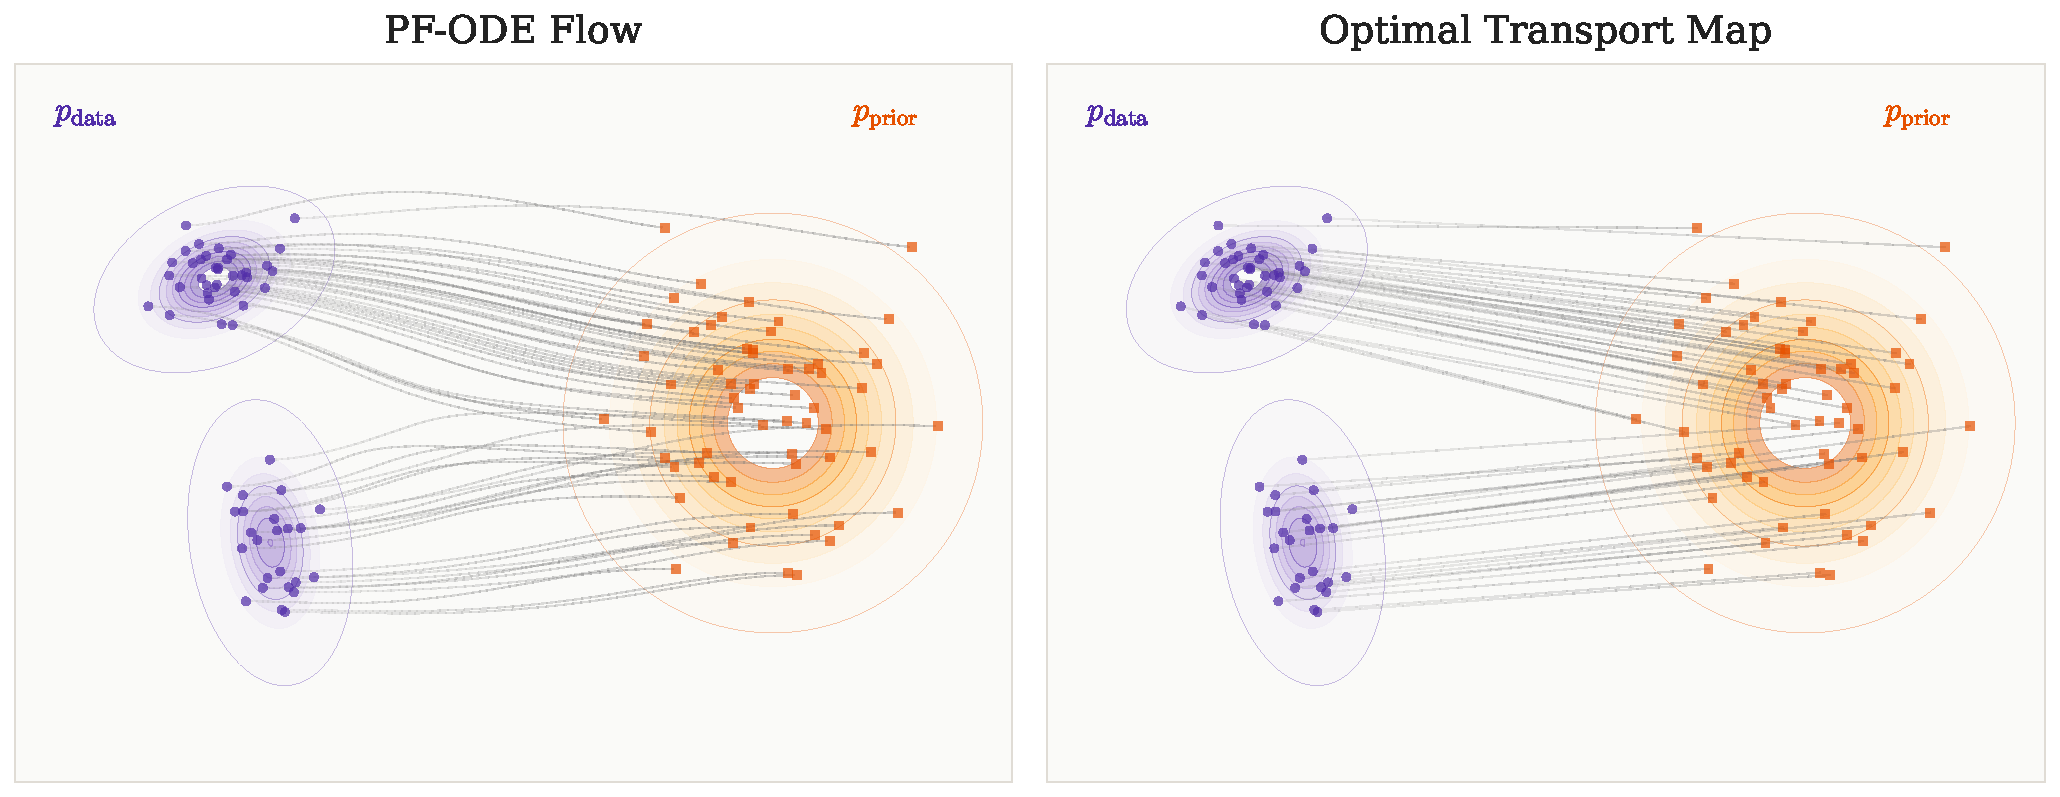
\includegraphics[width=\linewidth]{Images/PartB/pfode_vs_ot_2d.pdf}
    \caption{二维中从 $p_{\mathrm{data}}$ 到 $p_{\mathrm{prior}}$ 的 PF-ODE 流映射与真实 OT 映射的比较。
    右：二次代价 OT 映射，通过匈牙利算法精确计算。
    左：通过积分 PF-ODE 得到的 PF-ODE 流映射。两个映射明显不同，
    说明 PF-ODE 一般不能恢复最优传输映射。
    \figcredit{由作者在 AI 辅助编程下绘制。}}
    \label{fig:pfode-vs-ot-2d}
\end{figure}


\paragraph{设定。} 我们考虑 VP SDE，具体为 Ornstein–Uhlenbeck 过程，它将光滑初始密度 $p_0$ 演化为标准高斯 $\mathcal{N}(\bm{0}, \rmI)$：
\[
\diff \rvx(t) = -\rvx(t) \diff t + \sqrt{2} \diff \rvw(t), \quad \rvx(0) \sim p_0.
\]
相应的 PF-ODE 为
\[
\frac{\diff \mathbf{S}_t(\rvx)}{\diff t} = -\mathbf{S}_t(\rvx) - \nabla \log p_t(\mathbf{S}_t(\rvx)), \quad \mathbf{S}_0(\rvx) = \rvx.
\]
这里 $\mathbf{S}_t$ 表示将 $p_0$ 前推到边际 $p_t$ 的流映射：
\[
\left(\mathbf{S}_t\right) \# p_0 = p_t,
\quad\text{即}\quad
p_t(\rvy) = \int_{\mathbb{R}^D} \delta(\rvy - \mathbf{S}_t(\rvx))   p_0(\rvx) \diff \rvx.
\]
这些密度 $p_t$ 通过 Fokker-Planck 方程演化：
\[
\frac{\partial p_t}{\partial t} = \nabla \cdot (\rvx p_t) + \Delta p_t.
\]
这等价于具有如下速度场的连续性方程：
\[
\rvv_t(\rvx) = -\rvx - \nabla \log p_t(\rvx),
\]
其流由 $\mathbf{S}_t(\rvx)$ 给出。换言之，PF-ODE 可写为： 
\[
\frac{\diff \mathbf{S}_t(\rvx)}{\diff t} = \rvv_t\left(\mathbf{S}_t(\rvx)\right).
\]

当 $t \to \infty$ 时，该映射将初始分布传输到先验：
\[
\mathbf{S}_\infty \# p_0 = \mathcal{N}(\bm{0}, \rmI) =: p_{\text{prior}}.
\]
\paragraph{\citet{lavenant2022flow} 论证的目标。}

\citet{lavenant2022flow} 并不直接评估从 $p_0$ 到高斯的终端映射 $\mathbf{S}_\infty$ 是否最优。相反，他们构造一个特定的初始分布 $p_0$ 并考察整条 PF-ODE 轨迹。他们的关键观察是，最优性可能在流的某个点上失效。

他们考虑中间边际 $p_t = \mathbf{S}_t \# p_0$，并定义从 $p_{t_0}$ 到高斯的残差传输映射为
\[
\mathbf{T}_{t \to \infty} := \mathbf{S}_\infty \circ \mathbf{S}_{t}^{-1}, \quad \text{对所有 } t\geq 0.
\]
他们论证的核心是，对于精心选择的 $p_0$，存在一个时刻 $t_0 \geq 0$ 使得 $\mathbf{T}_{t_0 \to \infty}$ 不是从新的起始分布 $p_{t_0}$ 到 $\mathcal{N}(\bm{0}, \rmI)$ 的二次代价最优传输映射。

这一结果表明，PF-ODE 流一般并不产生最优传输映射，并且最优性这一性质对某些初始分布可能失效。

\paragraph{一些工具。} \citet{lavenant2022flow} 的论证关键依赖以下结果，即\emph{Brenier 定理}：
\begin{quote}
    \begin{theorem}[非正式的 Brenier 定理]\label{thm:brenier}
设 $\nu_1, \nu_2$ 为 $\mathbb{R}^D$ 上具有光滑密度的两个概率分布。一个光滑映射 $\rmT : \mathbb{R}^D \to \mathbb{R}^D$ 是从 $\nu_1$ 到 $\nu_2$（在二次代价下）的最优传输，当且仅当 $\rmT = \nabla u$，其中 $u$ 为某个凸函数。此时 $\mathrm{D} \rmT$ 对称且半正定，且 $u$ 满足 Monge–Ampère 方程：
\[
\det \mathrm{D}^2 u(\mathbf{x}) = \frac{\nu_1(\mathbf{x})}{\nu_2(\nabla u(\mathbf{x}))}.
\]
\end{theorem}
\end{quote}

证明还隐式地使用了如下事实，我们不再每次重复：\emph{一个映射是两个分布之间的最优传输，当且仅当其逆映射是反方向上的最优传输}。




\paragraph{证明梗概：PF-ODE 一般不是 OT 映射。} \citet{lavenant2022flow} 采用反证法：他们假设对每个 $t\ge0$，映射
\[
\mathbf{T}_t  =  \mathbf{S}_t \circ \mathbf{S}_\infty^{-1}
\]
是从 $\mathcal{N}(\bm{0},\rmI)$ 到 $p_t$ 的二次代价最优传输映射。




\subparagraph{第 1 步：Brenier 定理。}  由 Brenier 定理，从高斯出发的任何最优传输映射的雅可比必须对称且半正定。因此， 
\[
\mathrm{D} \mathbf{T}_t(\rvx) = \mathrm{D} \mathbf{S}_t(\mathbf{S}_\infty^{-1}(\rvx)) \mathrm{D} (\mathbf{S}_\infty^{-1})(\rvx)
\]
对所有 $t$ 和 $\rvx$ 必须对称。这里 $\mathrm{D} \mathbf{T}_t(\rvx)$ 表示关于 $\rvx$ 的全微分。
\subparagraph{第 2 步：对对称性条件关于时间求导。}  
关于时间求导：
\[
\frac{\partial}{\partial t} \mathrm{D}\mathbf{T}_t(\rvx)
= \left( \frac{\partial}{\partial t} \mathrm{D} \mathbf{S}_t \right)(\mathbf{S}_\infty^{-1}(\rvx)) \mathrm{D} (\mathbf{S}_\infty^{-1})(\rvx).
\]
鉴于对称性对所有 $t$ 成立，该导数也保持对称。

利用流 ODE（关于 $\rvx$ 求导），我们得到：
\[
\frac{\partial (\mathrm{D}\mathbf{S}_t)}{\partial t}
= \mathrm{D}\rvv_t(\mathbf{S}_t) \cdot \mathrm{D}\mathbf{S}_t
= \left( -\rmI - \mathrm{D}^2 \log p_t(\mathbf{S}_t) \right) \cdot \mathrm{D}\mathbf{S}_t.
\]
综合以上，我们看到
\[
\left( -\rmI - \mathrm{D}^2 \log p_t(\mathbf{S}_t) \right) \cdot\mathrm{D}\mathbf{S}_t \cdot \mathrm{D} (\mathbf{S}_\infty^{-1})
\]
对所有 $t\geq 0$ 对称。

在 $t = 0$ 处，我们有 $\mathbf{S}_0 = \rmI$ 且 $\mathrm{D}\mathbf{S}_0 = \rmI$，得到：
\[
\left( -\rmI - \mathrm{D}^2 \log p_0(\mathbf{S}_\infty^{-1}(\rvx)) \right) \cdot \mathrm{D} (\mathbf{S}_\infty^{-1})(\rvx) \quad \text{对称}.
\]

\subparagraph{第 3 步：交换性条件。}  由于假设 $\mathbf{T}_0 = \mathbf{S}_\infty^{-1}$ 是最优的，其雅可比 $D\mathbf{T}_0 = \mathrm{D}(\mathbf{S}_\infty^{-1})$ 对称。  此外，海森矩阵 $\mathrm{D}^2\log p_0$ 对称。  回顾两个对称矩阵相乘得到对称矩阵，当且仅当它们可交换。  因此，对所有 $\mathbf{x}\in\mathbb{R}^D$，
\[
\mathrm{D}^2\log p_0\bigl(\mathbf{S}_\infty^{-1}(\mathbf{x})\bigr)
\quad\text{必须与}\quad
\mathrm{D}(\mathbf{S}_\infty^{-1})(\mathbf{x})
\quad\text{可交换。}
\]
令 $\mathbf{y}=\mathbf{S}_\infty^{-1}(\mathbf{x})$ 得到等价条件：对所有 $\rvy\in\mathbb{R}^D$，
\[
\mathrm{D}^2\log p_0(\mathbf{y})
\quad\text{必须与}\quad
\mathrm{D}\mathbf{S}_\infty(\mathbf{y})
\quad\text{可交换。}
\]


现在，我们将这一条件转化为更可计算的形式。  
由于 $\mathbf{S}_\infty$ 在 $p_0$ 与 $\mathcal{N}(\bm{0},\rmI)$ 之间是最优的，Brenier 定理保证 $\mathbf{S}_\infty = \nabla u$，其中 $u$ 为某个凸函数。  由 Monge–Ampère 方程可得：
\[
\log p_0(\rvy) = \log \det(\mathrm{D}^2 u(\rvy)) - \frac{1}{2} \|\nabla u(\rvy)\|^2 + \text{Constant}.
\]
条件变为（其中 $\mathrm{D}\rmS_\infty = \mathrm{D}^2 u$）： 
\begin{mdframed}
\begin{align}\label{eq:necessary-ot}
\mathrm{D}^2 \left(\log \det \mathrm{D}^2 u - \frac{1}{2} \|\nabla u\|^2\right)
\quad\text{必须与}\quad
\mathrm{D}^2 u
\quad\text{可交换。}
\end{align}
\end{mdframed}
这给出了 $\mathbf{T}_t$ 为最优的一个必要条件。
\subparagraph{第 4 步：构造反例。} 让我们说明如何利用这一必要条件导出矛盾。

假设我们能构造一个凸函数 $u$ 使得  
\[
\mathrm{D}^2 \left( \log \det \mathrm{D}^2 u(\mathbf{x}) - \frac{1}{2} \lvert \nabla u(\mathbf{x}) \rvert^2 \right)
\]
不与 $\mathrm{D}^2 u(\mathbf{x})$ 对某个 $\mathbf{x} \in \mathbb{R}^D$ 可交换。  定义 $p_0 = (\nabla u)^{-1} \# \mathcal{N}(\bm{0}, \rmI)$，Brenier 定理蕴含 $\nabla u$ 是从 $p_0$ 到 $\mathcal{N}(\bm{0}, \rmI)$ 的最优传输。然而，\Cref{eq:necessary-ot} 中的条件失效，导致矛盾。因此，我们的目标是构造这样一个函数。 
考虑  
\[
u(\mathbf{x}) = \frac{1}{2} \|\mathbf{x}\|^2 + \varepsilon \phi(\mathbf{x}), \quad \text{对小的 } \varepsilon.
\]
则 $\mathrm{D}^2 u(\mathbf{0}) = \rmI + \varepsilon \mathrm{D}^2 \phi(\mathbf{0})$，且在 $\mathbf{x} = \mathbf{0}$ 处的可交换条件要求 $\mathrm{D}^2 \phi(\mathbf{0})$ 与 $\mathrm{D}^2 (\Delta \phi)(\mathbf{0})$ 可交换。 

例如，在 $\mathbb{R}^2$ 中，取  
\[
\phi(x_1, x_2) = x_1 x_2 + x_1^4
\]
便给出一个反例，其中海森矩阵 $\mathrm{D}^2 \log p_0$ 与雅可比 $\mathrm{D}^2 u$ 不可交换。

这一矛盾表明 $\mathbf{T}_t$ 不可能对所有 $t \geq 0$ 都最优。因此，存在某个 $t_0 \geq 0$ 使得映射 $\mathbf{T}_{t_0 \to \infty}$ 非最优。

\newpage 

\subsection{典型线性流与回流能否导出 OT 映射？}\label{subsec:ot-linear-reflow} 
我们已经看到 PF-ODE（尤其在前向核为 VP 型时）一般不是 OT 映射。现在一个自然的问题是：
\begin{question}
当将线性插值流 $(1-t)\rvx_0 + t \rvx_1$（其中 $\rvx_0\sim p_{\mathrm{src}}$、$\rvx_1\sim p_{\mathrm{tgt}}$）应用于独立耦合 $\pi(\rvx_0, \rvx_1) = p_{\mathrm{src}}(\rvx_0)p_{\mathrm{tgt}}(\rvx_1)$ 时，它能恢复 OT 映射吗？
\end{question}
问题的答案是否定的。
 
然而，将线性路径与给定耦合相结合，为真实 OT 代价提供了一个实用的上界。  在所有可能的路径中，线性插值提供了最紧的此类上界，正如我们在以下讨论中将看到的那样。


\paragraph{典型线性流与最优传输。}
聚焦于二次代价的最优传输，我们考虑 \Cref{eq:ot} 的等价形式，即 \Cref{eq:bb-ot} 中的 Benamou--Brenier 形式：
\begin{equation*}
    \mathcal{K}\left(p_{\mathrm{src}}, p_{\mathrm{tgt}}\right) :=  \min_{\substack{ (p_t, \rvv_t) \text{ s.t. }
        \partial_t p_t + \nabla \cdot (p_t \rvv_t) = 0, \\
        p_0 = p_{\mathrm{src}},\,\, p_1 = p_{\mathrm{tgt}}
    }}
    \int_0^1 \int_{\mathbb{R}^D} \|\rvv_t(\rvx)\|^2 p_t(\rvx) \diff\rvx \diff t.
\end{equation*}
不同于静态 Monge 形式（\Cref{eq: Monge's Formulation}），
其中计算最优映射需要求解 Monge--Amp\`ere
方程（\Cref{eq:monge-ampere}），Benamou--Brenier 问题在引入动量场
$\rvm_t := p_t \rvv_t$ 后允许一个凸重构。然而，将这一凸问题
在 $\mathbb{R}^D$ 的网格上离散化在高维下仍然不可处理。




虽然求解 Benamou-Brenier 形式一般不可行，但 \citet{liu2022rectified,lipman2024flow} 揭示其动能有一个实用的上界。这通过将搜索限制在更简单的\emph{条件流}族上来实现，其中每条路径由取自源分布与目标分布的某个耦合 $\pi_{0,1}$ 的固定端点 $(\rvx_0, \rvx_1)$ 定义。在这一\emph{条件流}族中，典型线性插值作为最优选择出现，如下面所形式化。

\proppp{通过条件流给出 OT 动能的上界}{ot-conditional-flow}{
设 $\pi_{0,1}$ 为 $p_{\mathrm{src}}$ 和 $p_{\mathrm{tgt}}$ 之间的任意耦合。
\begin{enumerate}
    \item[(1)] 动能以连接端点的任意条件流 $\bm{\Psi}_t(\rvx_0, \rvx_1)$ 的期望路径能量为上界：
    \begin{equation*}
        \mathcal{K}\left(p_{\mathrm{src}}, p_{\mathrm{tgt}}\right) \le \mathbb{E}_{(\rvx_0, \rvx_1) \sim \pi_{0,1}} \left[ \int_0^1 \|\bm{\Psi}'_t(\rvx_0, \rvx_1)\|^2 \diff t \right].
    \end{equation*}
    \item[(2)] 最小化右侧上界的唯一条件流 $\bm{\Psi}^*_t$ 是线性插值路径：
    \begin{equation*}
        \bm{\Psi}^*_t(\rvx_0, \rvx_1) = (1 - t) \rvx_0 + t \rvx_1.
    \end{equation*}
  代入这一最优路径得到最紧形式的上界：
    \begin{equation*}
        \mathcal{K}\left(p_{\mathrm{src}}, p_{\mathrm{tgt}}\right) \le \mathbb{E}_{(\rvx_0, \rvx_1) \sim \pi_{0,1}} \|\rvx_1 - \rvx_0\|^2.
    \end{equation*}
\end{enumerate}
}{证明依赖于 Jensen 不等式和条件期望的塔性质的直接应用，然后用 Euler-Lagrange 方程求解简化后的变分问题；完整论证参见 \citep{lipman2024flow} 的第 4.7 节。}

换言之，线性插值 $\bm{\Psi}^*_t$（即 Flow Matching 与 Rectified Flow 使用的前向核）对任意所选耦合 $\pi_{0,1}$，最小化了真实动能的一个上界。

我们强调，在此类条件流中的最优性并不保证在边际分布上的全局最优性。




\paragraph{回流与最优传输。} 
两个分布之间最朴素的传输方案，是使用简单的独立耦合以直线连接它们的样本。然而，这种方法明显不是最优的，因为问题不在于直线路径本身，而在于点的低效初始配对。

回流（Reflow）过程可能提供一种构造性的回应。它是一种专门为纠正这种配对而设计的迭代算法，并且关键是，每一步都保证代价非增 \citep{liu2022flow}。这一性质表明回流系统地将传输方案推向更优的配置，这自然地引出了关于其收敛性的核心问题。
\begin{question}
    如果我们迭代地应用 \texttt{Rectify} 算子会怎样？得到的传输方案序列能否收敛到最优方案，或者回流过程的不动点是否给出 OT 映射？
\end{question}
简短的答案在一般情况下是否定的。下面我们解释可能出什么问题。回顾一下，回流过程通过如下更新迭代地精炼 $p_{\mathrm{src}}$ 与 $p_{\mathrm{tgt}}$ 之间的耦合：
\[
\pi^{(k+1)} = \texttt{Rectify}(\pi^{(k)}),
\]
以乘积耦合 $\pi^{(0)} := p_{\mathrm{src}}(\rvx_0) p_{\mathrm{tgt}}(\rvx_1)$ 初始化。更确切地说，$\texttt{Rectify}$ 通过如下方式输出更新后的耦合 $\pi^{(k+1)}$：在每次迭代 $k = 0, 1, 2, \ldots$，通过如下方式学习一个速度场 $\rvv_t^{(k)}$：
\[
\rvv_t^{(k)} \in \argmin_{\rvu_t} \, \mathcal{L}(\rvu_t\big\vert\pi^{(k)}),
\]
其中 $\mathcal{L}(\rvu_t\big\vert\pi^{(k)})$ 是 \Cref{eq:reflow-loss} 中定义的损失（如 RF 或 FM 损失）。这里为记号简便，我们采用速度场的非参数形式，而非其他情形下使用的参数化形式 $\bm{\phi}$。
更新后的耦合由下式给出：
\[
\pi^{(k+1)}(\rvx_0, \rvx_1) := p_{\mathrm{src}}(\rvx_0)\, \delta\big(\rvx_1 - \bm{\Psi}_1^{(k)}(\rvx_0)\big),
\]
其中 $\bm{\Psi}_1^{(k)}$ 表示从初始条件 $\rvx_0$ 出发积分 $\rvv_t^{(k)}$ 在时间 $t=1$ 处得到的解映射。

在 \citep{liu2022flow} 中观察到，对于 $p_{\mathrm{src}}$ 与 $p_{\mathrm{tgt}}$ 之间的耦合 $\pi$，存在一个最小化回流损失的速度场 $\rvv_t$（即满足 $\mathcal{L}(\rvv_t |\pi) = 0$），这并不一定蕴含该传输是最优的。



受 Benamou–Brenier 框架（其中已知最优传输速度是某个势函数的梯度）启发，\citet{liu2022rectified} 提出了一个附加约束：速度场 $\rvv_t$ 应当是势场。相应地，\Cref{eq:reflow-loss} 中的目标被修改为将 $\rvv_t$ 限制在梯度向量场空间（也称为势流）中：
\begin{align}\label{eq:reflow-loss-gradient}
    \rvw_t^{(k)} \in \argmin_{\substack{\rvu_t:\, \rvu_t=\nabla\varphi \\ \text{对某个 }\varphi\colon\mathbb{R}^D\to\mathbb{R}}} \, \mathcal{L}(\rvu_t\big\vert\pi^{(k)}),
\end{align}
其余过程与 \texttt{Rectify} 中保持相同。
我们将这一相关算子记为 $\texttt{Rectify}_{\perp}$，强调其到无旋向量场的投影。

设 $\pi$ 为 $p_{\mathrm{src}}$ 与 $p_{\mathrm{tgt}}$ 之间的耦合。\citet{liu2022flow} 猜想如下刻画最优性的等价性：
\begin{enumerate}[label=(\textit{\roman*})]
  \item $\pi$ \textit{是最优传输耦合。}
  \item $\pi$ \textit{是势整流算子的不动点：}
  \[
    \pi = \texttt{Rectify}_{\perp}(\pi).
  \]
  \item \textit{存在一个梯度速度场 $\rvv_t = \nabla \varphi_t$ 使得整流损失为零：}
  \[
    \mathcal{L}(\rvv_t |\pi) = 0.
  \]
\end{enumerate}
然而，\citet{hertrich2025relation} 展示了两类反例：
\begin{enumerate}
  \item 当中间分布 $p_t$ 具有不连通支撑时，可以找到 $\texttt{Rectify}_{\perp}$ 的不动点，其回流损失为零且速度场为梯度场，但仍然无法产生最优耦合。
  \item 即使两个端点分布都是高斯分布，也存在损失任意小但偏离最优耦合任意大的耦合。
\end{enumerate}

因此，尽管整流流可能产生强大的生成模型，其作为最优传输求解器的可靠性仍然有限。这突显了生成建模与有原则的最优传输理论之间的重要差距，为二者交叉领域的进一步研究提供了契机。

最后，我们指出传输代价并不总是与下游性能相关；因此，计算精确的最优传输映射未必会带来更好的实际效果。尽管如此，最优传输的变体在科学与工程的许多问题中仍然具有基础性地位。扩散模型为探索这些挑战提供了一个强大的框架。

\newpage
\section{结束语}
在本章中，我们通过最优传输及其熵正则化变体的视角，重新审视了将一个
分布传输到另一个的经典问题。我们回顾了最优传输的静态
Monge--Kantorovich 形式与动态 Benamou--Brenier 形式，
其中传输由最小化动能代价的确定性流实现。随后我们讨论了熵正则化最优传输与
薛定谔桥（SB），它们用相对于参考过程最可能的受控扩散取代确定性传输。从
这一视角看，扩散模型在随机侧自然地接近 SB 的观点，
而其 PF-ODE 在 ODE 侧定义确定性
传输映射。然而，正如我们所强调的，PF-ODE
传输一般\emph{不是}二次代价最优传输
映射：它是众多确定性耦合之一，而非
Benamou--Brenier 作用量的最小化子。

这还突显了一个更基本的问题：在询问一个
传输是否最优之前，\emph{两个分布何时能完全由确定性映射连接？} 在许多设定下，存在性并非主要
困难。在温和的正则性假设下，常常能找到一个
可测映射 $\rmT$ 使得
$\rmT_\# p_{\mathrm{src}} = p_{\mathrm{tgt}}$。更困难的问题在于，
在一维以上，相对较少的经典构造既
显式又在实践中稳健。在一维中，单调
重排通过匹配分位数给出简单答案。在高维中，已知若干重要构造：Brenier 定理
（定理~\ref{thm:brenier}）在适当正则性下给出二次代价最优映射；Knothe--Rosenblatt
重排~\citep{rosenblatt1952remarks,knothe1957contributions}
由迭代的条件分布构造三角映射；而
Dacorogna--Moser 方法~\citep{dacorogna1990partial} 通过求解散度
方程的速度场构造光滑
微分同胚传输。每种方法都给出有原则的确定性传输途径，但
也都依赖于结构性假设或非平凡的分析
工具。

从这一视角看，基于扩散的流映射提供了一种有吸引力且
灵活的替代方案。扩散模型与流匹配方法不规定一个闭式传输
映射，而是学习一个随时间变化的
向量场，其诱导流将一个简单源分布推向
目标。这种学习到的映射不必与 Brenier
映射或任何其他经典的典型构造重合，且一般而言它
并不求解预定的最优传输问题。尽管如此，它
提供了一条实用且富有表达力的途径，用于高维下基于映射的采样，而那里
显式传输映射构造常常
不可用或难以计算。在这个意义上，扩散流最好
不被理解为经典传输理论的替代品，而是
现代学习到的传输机制，与最优
传输映射、三角重排以及基于 PDE 的构造
并列存在于确定性传输的更广阔图景之中。
\newpage

\part{扩散模型的采样}

\vspace*{\fill}  % push content down
\begin{figure*}[th!]
\begin{center}
\resizebox{\textwidth}{!}{% 
\centering
\begin{tikzpicture}[
    box/.style={rectangle, draw, thick, minimum width=3cm, minimum height=2cm, align=center},
    topbox/.style={rectangle, draw, thick, minimum width=12cm, minimum height=1.5cm, align=center},
    arrow/.style={->, thick},
    roundbox/.style={rectangle, draw, thick, rounded corners=10pt, minimum width=4cm, minimum height=3cm, align=center}
]

% Top box
\node[topbox, label=above:{\parbox{5cm}{\centering  {第}~\ref{ch:score-sde}~{章}}}] (top) at (0,4) {\\
\textbfs{使用扩散模型 $\mathbf{v}^*(\rvx, t)$ 生成} \\[0.3cm]
$\Longleftrightarrow$ 在 $\mathbf{x}(T)\sim p_{\mathrm{prior}}$ 下从 $T$ 到 $0$ 反向求解 ODE（更一般地，从 $s$ 到 $t$，其中 $s>t$）：\\[0.2cm]
$\displaystyle\frac{\diff\mathbf{x}(t)}{\diff t} = \mathbf{v}^*(\mathbf{x}(t), t)$ \\[0.3cm]
$\displaystyle\Longleftrightarrow \mathbf{x}(0) = \mathbf{x}(T) + \int_0^T \mathbf{v}^*(\mathbf{x}(t), t)\diff t$
};

% Three bottom boxes
\node[roundbox, label=below:{\parbox{5cm}{\centering  {第}~\ref{ch:guidance}~{章}
 }}] (left) at (-6,-2) {
\\ \large\textbfs{引导生成} \\[0.4cm]
\parbox{5cm}{
\begin{align*}
    \displaystyle\mathbf{x}(0) &= \mathbf{x}(T) + \int_0^T [\mathbf{v}^*(\mathbf{x}(t), t) \\ 
    &\qquad \textcolor{darkgray}{+ \textbf{引导}}] \diff t
\end{align*}}
};

\node[roundbox, label=below:{\parbox{5cm}{\centering {第}~\ref{ch:solvers}~{章}
 }}] (center) at (0,-2) {
\\ \large\textbfs{快速生成} \\
\large\textbfs{与数值求解器} \\[-0.6cm]
$\displaystyle\mathbf{x}(0) = \mathbf{x}(T) + \eqnmarkbox[Plum]{velocity}{\int_0^T \mathbf{v}^*(\mathbf{x}(t), t)\diff t}$ \\[-0.8cm]
估计积分
};

\node[roundbox, label=below:{\parbox{5cm}{\centering  {第}~\ref{ch:distillation}~{章} {和} {第}~\ref{ch:fast-scratch}~{章}
 }}] (right) at (6,-2) {
\\ \large\textbfs{学习快速的} \\
\large\textbfs{扩散生成器} \\[-0.6cm]
$\displaystyle\mathbf{x}(0) = \eqnmarkbox[Pink]{target}{\mathbf{x}(T) + \int_0^T \mathbf{v}^*(\mathbf{x}(t), t)\diff t}$ \\[-0.8cm]
学习积分
};

% Arrows
\draw[ultra thick, -{Stealth[length=4mm, width=4mm]}, rounded corners=4pt] (top.south) -- ++(-6,-1) -- (left.north);
\draw[ultra thick, -{Stealth[length=4mm, width=4mm]}, rounded corners=4pt] (top.south) -- (center.north);
\draw[ultra thick, -{Stealth[length=4mm, width=4mm]}, rounded corners=4pt] (top.south) -- ++(6,-1) -- (right.north);

\end{tikzpicture}
}
\end{center}
% \label{fig:part-c-d-roadmap}
\end{figure*}
\vspace*{\fill}  % push content up

\chapter{引导与可控生成}\label{ch:guidance}
扩散模型是强大的生成式框架。在无条件设定下，目标是学习 $p_{\text{data}}(\rvx)$ 并在没有外部输入的情况下生成样本。

然而，许多应用需要\emph{条件生成}，即输出须满足用户指定的标准。这可以通过对无条件模型进行引导，或者直接学习条件分布 $p_0(\rvx | \rvc)$ 来实现，其中条件 $\rvc$（例如标签、文本描述或草图）引导整个过程。

本章基于条件分数的一个原则性视角，该视角将条件分数分解为一个\emph{无条件方向}和一个\emph{引导方向}：前者在保持真实性的同时将样本推向所给条件。我们将解释为何引导是必不可少的，说明条件分数如何作为统一的控制接口，并综述近似引导项的多种方法。随后，我们将区分\emph{控制}（满足条件）与\emph{对齐}（在给定条件下满足人类偏好），并阐述如何将偏好纳入同一框架。最后，我们讨论在无需额外奖励模型（即一个学习得到的评分器，它对与人类偏好更一致的输出赋予更高的值）的情况下直接优化偏好。




\clearpage
\newpage

\section{引言}\label{sec:prologue-guidance}


\begin{figure}[th!]
    \centering
    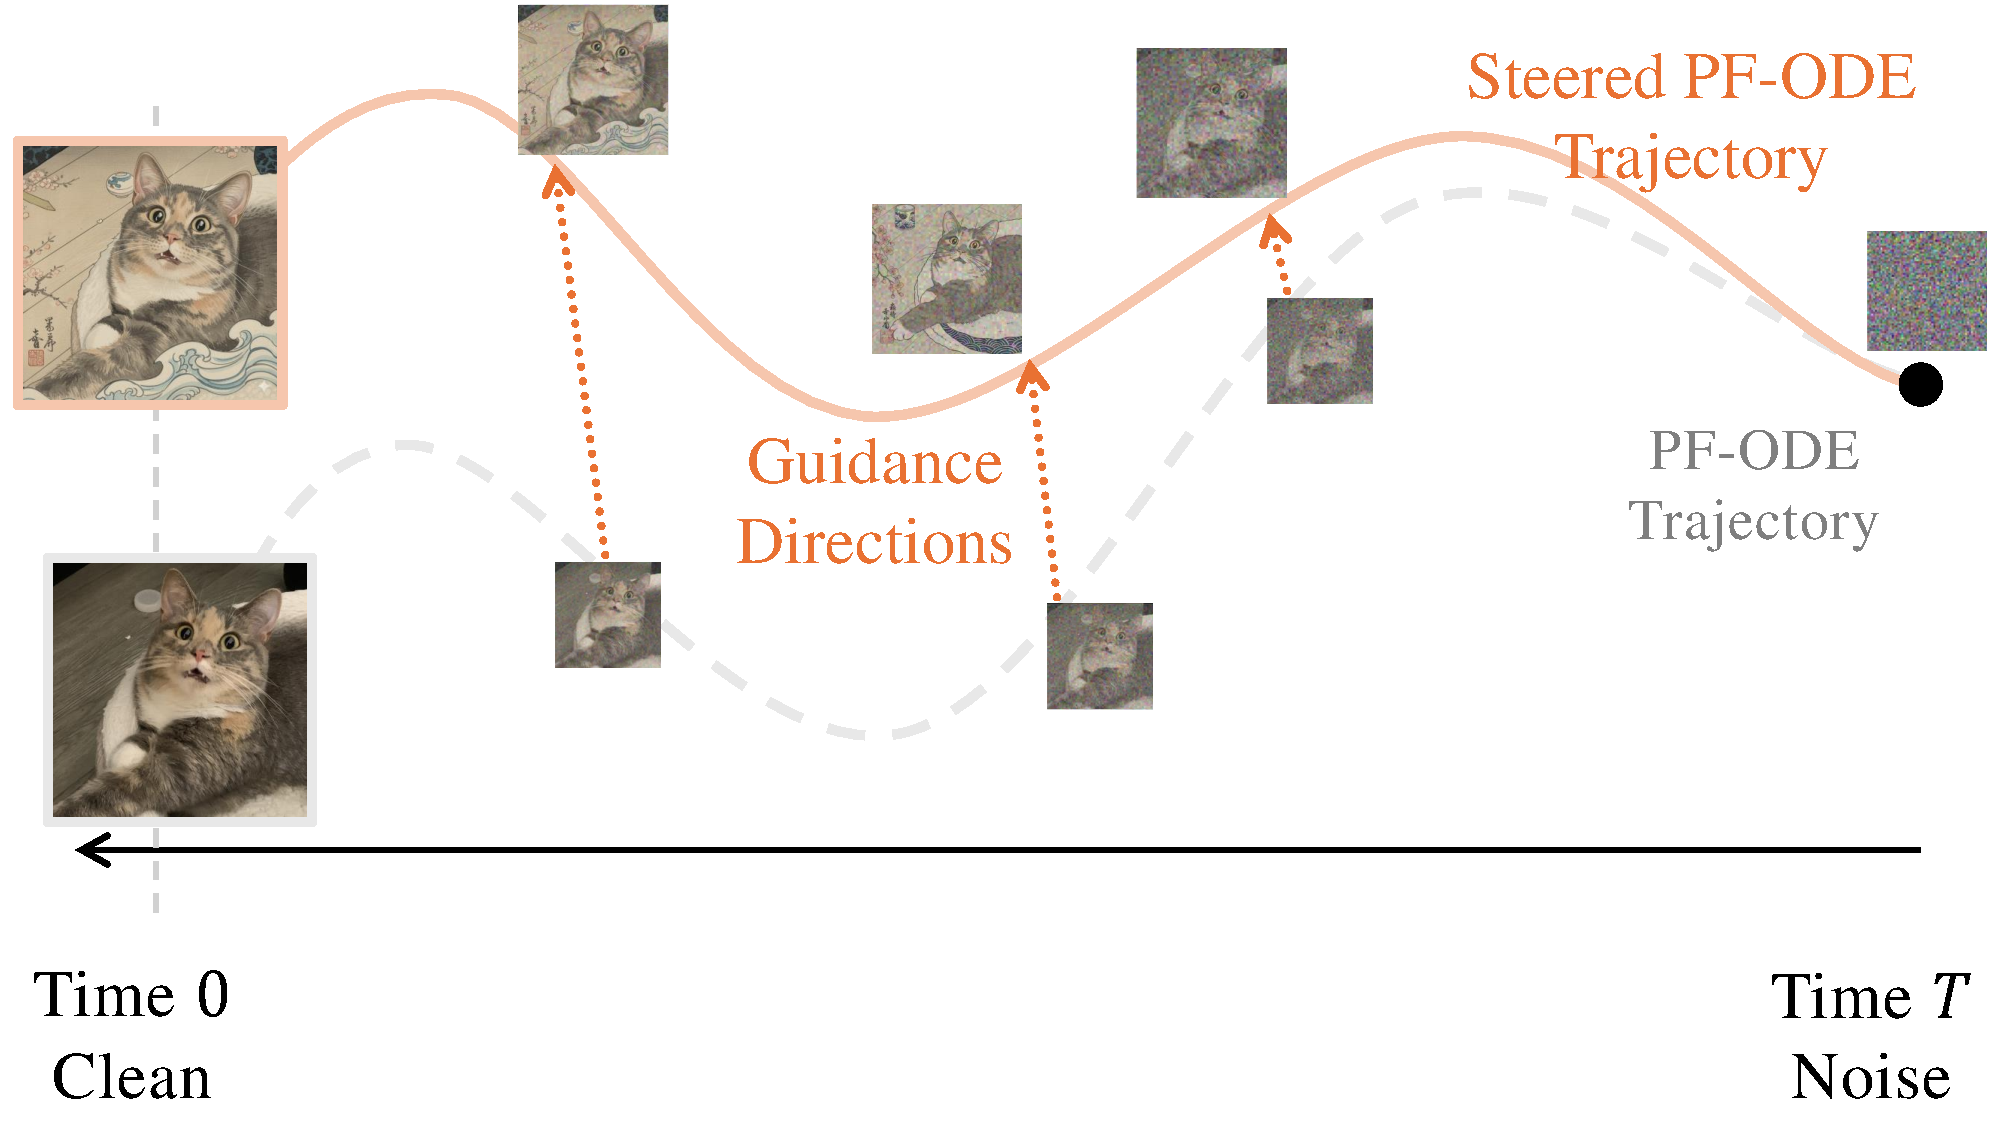
\includegraphics[width=\linewidth]{Images/PartC/guidance.pdf}
\caption{\textbfs{引导扩散采样的示意图。}
逆向时间 PF-ODE 采样从右侧的纯噪声（$t = T$）开始，逐步演化为左侧（$t = 0$）的清晰样本。
在此过程中，由 $w_t$ 加权的引导方向 $\nabla_{\rvx_t}\log \tilde{p}_t(\rvc |\rvx_t)$ 按照下式修改速度场：
$\nabla_{\rvx_t}\log p_t(\rvx_t) + w_t\,\nabla_{\rvx_t}\log \tilde{p}_t(\rvc |\rvx_t)$。
这些额外的方向在样本由粗到细逐步精化的同时，将轨迹引向目标属性（日本绘画风格）。
\figcredit{由作者绘制。}}
    \label{fig:guidance}
\end{figure}


扩散模型的生成过程以由粗到细的方式进行，为可控生成提供了灵活的框架。在每一步中，少量噪声被移除，样本变得更加清晰，逐渐显现出更多的结构和细节。这一特性使我们可以对生成过程进行控制：通过在所学到的、随时间变化的速度场上添加一个引导项，我们可以引导生成轨迹反映用户的意图。

扩散模型中基于引导的采样的一个原则性基础是条件分数的贝叶斯分解。对于每个噪声水平 $t$，
\begin{mdframed}
\begin{align}
\nabla_{\rvx_t}\log p_t(\rvx_t |\rvc)
=
\underbrace{\nabla_{\rvx_t}\log p_t(\rvx_t)}_{\text{无条件方向}}
+
\underbrace{\nabla_{\rvx_t}\log p_t(\rvc |\rvx_t)}_{\text{引导方向}}.
\label{eq:guidance_bayes}
\end{align}
\end{mdframed}
这一恒等式表明，条件采样可以通过在无条件分数之上添加一个引导项 $\nabla_{\rvx_t}\log p_t(\rvc |\rvx_t)$ 来实现。由于 $p_t(\rvc |\rvx_t)$ 通常因为要对 $\rvx_0$ 进行边缘化而难以处理，各种可控生成方法（例如分类器引导~\citep{dhariwal2021diffusion}、通用的免训练引导~\citep{ye2024tfg}）都可以解释为对该引导项的不同近似。

一旦获得了这样的近似，采样只需用条件分数替代无条件分数即可。利用 \Cref{eq:guidance_bayes}，PF-ODE 变为
\begin{align}\label{eq:condition_prob_ode}
\begin{aligned}
    \frac{\diff \mathbf{x}(t)}{\diff t} &= f(t)\mathbf{x}(t) - \frac{1}{2} g^2(t) \underbrace{\nabla_{\rvx_t} \log p_t(\rvx(t) |\rvc)}_{\text{条件分数}} \\
    &= f(t)\mathbf{x}(t) - \frac{1}{2} g^2(t) \Big[ \nabla_{\rvx_t} \log p_t(\rvx(t)) + \nabla_{\rvx_t} \log p_t(\rvc |\rvx(t)) \Big].
\end{aligned}
\end{align}
我们强调，引导这些随时间变化的向量场从根本上依赖于它们的线性性，因此下文以分数预测形式给出的讨论，可通过 \Cref{eq:predictions-equivalence} 中的线性关系自然地推广到 $\rvx$-、$\beps$- 和 $\rvv$-预测。

\paragraph{引导方向的具体形式。}
\begin{enumerate}[leftmargin=*]
\item \textbfs{分类器引导（CG）。} 在 \Cref{sec:cg} 中，分类器引导（CG）在加噪数据 $\rvx_t$（通过在水平 $t$ 上破坏带标签的干净样本得到）上训练一个时间条件分类器
$p_{\bpsi}(\rvc | \rvx_t, t)$。在采样时，其输入梯度提供引导项：
\[
\nabla_{\rvx_t}\log p_{\bpsi}(\rvc | \rvx_t, t)
 \approx  \nabla_{\rvx_t}\log p_t(\rvc | \rvx_t),
\]
随后将其加到无条件分数上~\citep{dhariwal2021diffusion}。
\item \textbfs{无分类器引导（CFG）。} 在 \Cref{sec:cfg} 中，CFG 直接训练单个条件模型
\[
\rvs_{\bphi}(\rvx_t,t,\rvc) \approx \nabla_{\rvx_t}\log p_t(\rvx_t|\rvc),
\]
其中无条件模型是通过在部分训练步骤中以一个特殊的空标记随机替换条件来联合学习的。
\item \textbfs{免训练（替代）引导。}  条件分布 $p_t(\rvc| \rvx_t)$ 通常难以处理，因为它需要对干净隐变量 $\rvx_0$ 进行边缘化：
\[
p_t(\rvc| \rvx_t)
= \int p(\rvc| \rvx_0)  p(\rvx_0| \rvx_t)  \mathrm d\rvx_0,
\]
而且在典型应用中，至少有一个因子是未知的，使得该积分难以计算。

在 \Cref{subsec:tfg} 中，免训练（基于损失的）引导避免直接评估条件似然 $p_t(\mathbf{c}| \mathbf{x}_t)$。
相反，它引入一个现成的损失 $\ell(\mathbf{x}_t,\mathbf{c};t)$
并将替代条件分布 $\widetilde p_t(\mathbf{c}|\mathbf{x}_t) $ 定义为
\[
\widetilde p_t(\mathbf{c}|\mathbf{x}_t) \propto \exp\!\big(-\tau\,\ell(\mathbf{x}_t,\mathbf{c};t)\big),
\quad \tau>0,
\]
它充当一个伪似然。
这一表述规避了计算真实条件似然的困难，同时仍然可以通过所选损失的梯度实现引导。其条件分数仅由带有 $\tau$ 的损失梯度计算：
\[
\nabla_{\rvx_t}\log \widetilde p_t(\rvc|\rvx_t)
= -\tau \nabla_{\rvx_t}\ell(\rvx_t,\rvc; t).
\]
这一项以引导权重 $w_t$ 加到无条件分数上：
\[
  \nabla_{\rvx_t}\log p_t(\rvx_t)
 + w_t \bigl[-\tau \nabla_{\rvx_t}\ell(\rvx_t,\rvc; t)\bigr].
\]
这恰好是 \emph{倾斜}密度 $\widetilde p_t^{\mathrm{tilt}}(\rvx_t| \rvc)$ 的分数，定义为：
\[
\widetilde p_t^{\mathrm{tilt}}(\rvx_t| \rvc) \propto  p_t(\rvx_t) \widetilde p_t(\rvc| \rvx_t)^{w_t}
 \propto  p_t(\rvx_t) \exp\!\big(-w_t\tau \ell(\rvx_t,\rvc; t)\big).
\]
在实践中，我们将 \Cref{eq:condition_prob_ode} 中采样的条件分数替换为该倾斜分数，并求解所得的 ODE 来抽取样本。

鉴于此，分类器引导只是用一个学习得到的分类器 $\widetilde p_t(\mathbf{c}|\mathbf{x}_t):=p_{\bpsi^\times}(\rvc| \rvx_t,t)$ 实现的替代引导，即：
\[
\ell(\rvx_t,\rvc; t) = -\log p_{\bpsi^\times}(\rvc| \rvx_t,t), \quad \tau=1.
\]

引导对采样轨迹的影响如 \Cref{fig:guidance} 所示。

所有这些技术同样可以叠加到条件模型之上，
从而允许在生成过程中注入额外的控制信号。

\end{enumerate}
\rmkb{引导 PF-ODE（一般而言）\emph{并不}从倾斜分布族中采样。
即便分数完全精确、ODE 积分也完全精确，将分数替换为\emph{倾斜}分数并不能使时间 $t$ 的边缘分布等于
$\{\widetilde p_t^{\mathrm{tilt}}(\cdot|\rvc)\}_{t\in[0,1]}$，也不能使终止分布等于
$\widetilde p_0^{\mathrm{tilt}}(\cdot|\rvc)$。

定义
\[
\rvv_t^{\mathrm{orig}} = \rvf - \tfrac12 g^2(t) \nabla \log p_t, \quad
\rvh_t(\rvx)=e^{-w_t\tau \ell(\rvx,\rvc;t)}, \quad
\widetilde p_t^{\mathrm{tilt}}=\tfrac{p_t \rvh_t}{Z_t}.
\]
引导后的 PF-ODE 使用
\[
\rvv_t^{\mathrm{tilt}} = \rvf - \tfrac12 g^2(t) \nabla \log \widetilde p_t^{\mathrm{tilt}}
= \rvv_t^{\mathrm{orig}} - \tfrac12 g^2(t) \nabla \log \rvh_t.
\]

如果 $\widetilde p_t^{\mathrm{tilt}}$ 是真实的边缘分布，它们应满足
\[
\partial_t \widetilde p_t^{\mathrm{tilt}} + \nabla\!\cdot(\widetilde p_t^{\mathrm{tilt}} \rvv_t^{\mathrm{tilt}})=0.
\]
但直接计算得到残差
\begin{align*}
    &\partial_t \widetilde p_t^{\mathrm{tilt}} + \nabla \cdot(\widetilde p_t^{\mathrm{tilt}}  \rvv_t^{\mathrm{tilt}})
\\= &\widetilde p_t^{\mathrm{tilt}} \Big[ \partial_t \log \rvh_t
+ \rvv_t^{\mathrm{orig}} \cdot\nabla \log \rvh_t
- \tfrac12 g^2(t) \big(\Delta \log \rvh_t + \|\nabla \log \rvh_t\|^2 \big)
- \tfrac{Z_t'}{Z_t} \Big].
\end{align*}

因此，$\widetilde p_t^{\mathrm{tilt}}$ 与 PF-ODE 的边缘分布相吻合，当且仅当对所有 $\rvx$ 括号中的项为零，即
\[
\partial_t \log \rvh_t + \rvv_t^{\mathrm{orig}} \cdot\nabla \log \rvh_t
= \tfrac12 g^2(t)\big(\Delta \log \rvh_t + \|\nabla \log \rvh_t\|^2\big) + \tfrac{Z_t'}{Z_t}.
\]
这一条件在 $w_t\equiv 0$（无条件生成）时平凡地成立，但对
$\rvh_t(\rvx)=e^{-w_t\tau\ell(\rvx,\rvc;t)}$ 几乎从不成立，除非 $w_t$ 或 $\ell$ 处于非常特殊的情况。因此，一般而言
$\{\widetilde p_t^{\mathrm{tilt}}\}$ \emph{并非} PF-ODE 的边缘分布，终止样本\emph{并不}服从 $\widetilde p_0^{\mathrm{tilt}}(\rvx_0|\rvc)$ 分布。这一视角在精神上也与 \citep{lai2023fp} 相关。


对于希望超越这种启发式引导的读者，基于校正的方法~\citep{skreta2025feynman}，例如 Feynman--Kac 校正子，旨在显式地补偿引导后的动力学与所期望的倾斜分布之间的不匹配，使采样在整个轨迹中更忠实地遵循目标分布族。

}




% If an additional attribute $\tilde{\rvc}$ is desired under a base condition $\rvc$, one can stacking or refining conditions
% \begin{align*}
%     \nabla_{\rvx_t}\log p_t(\rvx_t | \rvc,\tilde{\rvc})
% &=
% \nabla_{\rvx_t}\log p_t(\rvx_t | \rvc)
% +
% \nabla_{\rvx_t}\log p_t(\tilde{\rvc}| \rvx_t,\rvc)
% \\&\approx
% \rvs_{\bphi^\times}(\rvx_t,t,\rvc) - \nabla_{\rvx_t}\ell(\rvx_t,\rvc,\tilde{\rvc};t),
% \end{align*}
% so one can compose controls by adding further surrogate guidance terms.

\paragraph{从控制到与直接偏好优化的更好对齐。}
强控制可能满足条件却偏离偏好：一个样本可能满足条件化信号（例如提示），却偏离人类真正偏好的结果。我们通过对条件目标按偏好评分进行\emph{倾斜}来形式化这一点\footnote{我们指出，免训练引导也可以视为在损失 $\ell(\rvx_t, \rvc, t)$ 引导下寻找倾斜分布的同一框架。}：
\[
\widetilde p_0^{\mathrm{tilt}}(\rvx_0| \rvc) \propto p_0(\rvx_0|\rvc) \exp \big(\beta r(\rvx_0,\rvc)\big),
\]
其中 $r(\rvx_0,\rvc)$ 是对干净样本 $\rvx_0$ 和条件 $\rvc$ 给出的标量对齐评分（奖励）（$r$ 越大表示对齐越好）。在实践中，$r$ 可以是 (i) 外部奖励/分类器的 logit 或对数概率，(ii) 相似性度量（例如 CLIP/感知相似度~\citep{radford2021learning}），或 (iii) 学习得到的偏好模型。

% \subparagraph{Training-Free Method and Its Relation to Training-Free Guidance.}
% At intermediate times, the tilted marginals $\tilde{p}_t(\rvx_t|\rvc)$ satisfy
% \[
% \nabla_{\rvx_t}\log \tilde{p}_t(\rvx_t|\rvc)
% =
% \nabla_{\rvx_t}\log p_t(\rvx_t|\rvc)
% +
% \nabla_{\rvx_t}\log \E \left[\exp \big(\beta r(\rvx_0,\rvc)\big) |dle|  \rvx_t,\rvc\right],
% \]
% where the conditional expectation is under the base posterior $p(\rvx_0|\rvx_t,\rvc)$. For small $\beta$, a first-order cumulant expansion gives
% \[
% \nabla_{\rvx_t}\log \tilde{p}_t(\rvx_t|\rvc)
% \approx
% \nabla_{\rvx_t}\log p_t(\rvx_t|\rvc)
% + \underbrace{\beta \nabla_{\rvx_t}\E \left[r(\rvx_0,\rvc)|\rvx_t,\rvc\right]}_{\mathrm{alignment\ guidance}}
% \quad(+ \mathcal O(\beta^2)).
% \]
% Thus alignment guidance adds the gradient of a posterior preference potential. To connect with training-free guidance, define a pseudo-likelihood
% \[
% p_t(\rvc|\rvx_t) \propto \exp \big(-\ell(\rvx_t,\rvc,t)\big),
% \quad
% \ell(\rvx_t,\rvc,t) := - \beta \E \left[r(\rvx_0,\rvc)|\rvx_t,\rvc\right],
% \]
% which yields the same leading-order term
% \[
% -\nabla_{\rvx_t}\ell = \beta \nabla_{\rvx_t}\E \left[r|\rvx_t,\rvc\right].
% \]
% In particular, choosing $r(\rvx_0,\rvc)=\log p(\rvc|\rvx_0)$ and taking the expectation under the \emph{unconditional} posterior $p(\rvx_0|\rvx_t)$ (i.e., using an unconditional base model with the condition as a likelihood) gives
% \[
% \nabla_{\rvx_t}\log \E \big[e^{r(\rvx_0,\rvc)}|\rvx_t\big]
% = \nabla_{\rvx_t}\log p_t(\rvc|\rvx_t)
% \]
% by Bayes' rule, recovering the classic training-free guidance decomposition
% $
% \nabla_{\rvx_t}\log p_t(\rvx_t|\rvc)
% = \nabla_{\rvx_t}\log p_t(\rvx_t) + \nabla_{\rvx_t}\log p_t(\rvc|\rvx_t).
% $
% Conceptually, we will treat alignment guidance and training-free guidance under a unified view (they coincide to first order in $\beta$). In practice, the conditional expectation is intractable and is typically approximated (e.g., via a denoised $\hat{\rvx}_0$ or a proxy classifier/reward head).


实现此类可引导性的现有方法通常收集关于模型生成相对质量的人类标签，并通过人类反馈强化学习（RLHF）对条件扩散模型进行微调以与这些偏好对齐。然而，RLHF 是一个复杂且常常不稳定的过程：它首先拟合一个奖励模型来捕捉人类偏好，然后用强化学习微调条件扩散模型，以最大化这一估计的奖励，同时约束策略相对于原始模型的漂移。

这自然引出了一个问题：\emph{我们能否完全移除奖励模型的训练阶段？}我们用 Diffusion-DPO~\citep{wallace2024diffusion} 来回答这个问题，它是对最初为大语言模型开发的直接偏好优化~\citep{rafailov2023direct} 的一种改编。如 \Cref{sec:rlhf-dpo} 所述，Diffusion-DPO 直接从成对选择中学习偏好倾斜，因此条件扩散模型无需单独的奖励模型即可微调以对齐偏好。




% A principled foundation for guidance-based sampling in diffusion models arises from the Bayesian decomposition of the conditional score function. According to Bayes' rule, the conditional score at each time slice can be decomposed as (see \Cref{eq:cg-density-omega} for details):
% \begin{mdframed}
%     \begin{align}
% \nabla_{\rvx_t} \log p_t(\rvx_t | \rvc) = \underbrace{\nabla_{\rvx_t} \log p_t(\rvx_t)}_{\text{uncond. direction}}
% + \underbrace{\nabla_{\rvx_t} \log p_t(\rvc | \rvx_t)}_{\text{guidance direction}}, \label{eq:guidance_bayes}
% \end{align}
% \end{mdframed}
% where $\nabla_{\rvx_t} \log p_t(\rvc | \rvx_t)$ represents a guidance signal that encourages the generation to align with the desired condition.

% Many works aiming to steer diffusion models toward conditional generation are fundamentally based on the identity in \Cref{eq:guidance_bayes}. More precisely, with the conditional score $\nabla_{\rvx_t} \log p_t(\rvx_t | \rvc)$, the original unconditional formulation in the reverse-time SDE (\Cref{eq:sde_backward}) or the PF-ODE (\Cref{eq:prob_ode_gt}) can be adapted for conditional sampling to generate from the target distribution $p_0(\rvx_0 | \rvc)$ by numerically solving the differential equations. Taking the PF-ODE formulation as an example, we have:
% \begin{align}\label{eq:condition_prob_ode}
% \begin{aligned}
%     \frac{\diff \mathbf{x}(t)}{\diff t} &= f(t)\mathbf{x}(t) - \frac{1}{2} g^2(t) \underbrace{\nabla_{\rvx_t} \log p_t(\rvx(t) | \rvc)}_{\text{conditional score}} \\
%     &= f(t)\mathbf{x}(t) - \frac{1}{2} g^2(t) \left[ \nabla_{\rvx_t} \log p_t(\rvx(t)) + \nabla_{\rvx_t} \log p_t(\rvc | \rvx(t)) \right],
% \end{aligned}
% \end{align}
% with initialization $\rvx_T \sim p_{\rm prior}$\footnote{For sufficiently large $T$ and appropriately designed $f(t)$, $p(\rvx_T | \rvc) \approx p_{\rm prior}(\rvx_T)$ is approximately Gaussian independent of $\rvc$.}.

% The most naive method is


% \newpage
% Existing methods can be broadly categorized into two classes, depending on whether additional training of the generative model is required:


% \paragraph{Training-Based Approaches.} These methods require training or fine-tuning a conditional generative model on paired data $(\rvx_0, \rvc)$. Unlike traditional generative models, such as conditional GANs \citep{mirza2014conditional} which directly learn a conditional mapping $\rmG_{\bm{\phi}}(\rvz, \rvc)$ with $\rvz \sim p(\rvz)$, diffusion-based approaches must account for the temporal nature of the sampling process.

% In this setting, the reverse-time dynamics are explicitly conditioned on the external signal $\rvc$. A typical approach is to train a conditional score network,
% \[
% \rvs_{\bm{\phi}}(\rvx_t, t, \rvc) \approx \nabla_{\rvx_t} \log p_t(\rvx_t | \rvc),
% \]
% using score-matching or denoising objectives. Once trained, the conditional score is used to simulate the reverse-time SDE or its deterministic equivalent to generate samples aligned with $\rvc$.

% Notable techniques include:
% \begin{itemize}
%     \item \textbfs{Classifier Guidance (CG).} CG~\citep{dhariwal2021diffusion}  uses an external classifier to estimate $\nabla_{\rvx_t} \log p_t(\rvc | \rvx_t)$.
%     \item \textbfs{Classifier-Free Guidance (CFG).} CFG~\citep{ho2021classifier}  directly trains the model to operate under both conditional and unconditional settings, allowing interpolation between the two during generation.
% \end{itemize}

% \paragraph{Training-Free Approaches.} These methods operate without modifying or retraining the diffusion model. Instead, they utilize a pre-trained unconditional model to approximate $\nabla_{\mathbf{x}_t} \log p_t(\mathbf{x}_t)$. In addition, the guidance term $\nabla_{\mathbf{x}_t} \log p_t(\mathbf{c} | \mathbf{x}_t)$ is estimated at inference time using task-specific information, as it is generally intractable to compute in closed form due to its dependence on the marginal
% \[
% p_t(\mathbf{c} | \mathbf{x}_t) = \int p(\mathbf{c} | \mathbf{x}_0)   p(\mathbf{x}_0 | \mathbf{x}_t)   \diff \mathbf{x}_0.
% \]
% This class of methods is particularly flexible and broadly applicable. For instance:
% \begin{itemize}
%     \item In inverse problems, the guidance term can be derived from a data-fidelity term or likelihood of observed measurements.
%     \item In controllable generation, the gradient can be computed from pre-trained attribute classifiers or target embedding similarity. Guidance can also be formulated based on large language models or retrieval-based objectives.
% \end{itemize}

% By appropriately approximating the guidance term, one can steer a fixed diffusion model toward a variety of target distributions, all without retraining.


% \paragraph{From Guidance to Alignment: Why CFG Is Not Enough.}
% \Cref{eq:guidance_bayes} shows that conditional sampling can be steered by a guidance term $\nabla_{\rvx_t}\log p_t(\rvc|\rvx_t)$.
% This signal enforces the \emph{specified condition} (class label, text prompt, measurement model, etc.), but it does not, by itself, guarantee that the resulting samples match \emph{human preferences} (style, safety, non-toxicity, aesthetic quality, faithfulness beyond the literal prompt,~\emph{etc.}).
% In practice, even strong controllable generation (CG)---including classifier guidance and classifier-free guidance (CFG)---may still yield artifacts that are technically on-condition yet misaligned with what users actually prefer.
% This motivates a second layer of control: \emph{alignment}, where we reshape the conditional distribution toward human-preferred outputs.

% \paragraph{A Principled View: Preference-Tilted Targets.}
% Let $p_0(\rvx_0|\rvc)$ denote the conditional distribution reachable by CG/CFG.
% Alignment asks for a preference-tilted target
% \begin{equation}\label{eq:pref_tilt}
% \tilde{p}_0(\rvx_0|\rvc) \propto p_0(\rvx_0|\rvc) \exp \big(\beta  r^\star(\rvx_0,\rvc)\big),
% \end{equation}
% where $r^\star(\rvx_0,\rvc)$ is a (unknown) preference score and $\beta>0$ controls strength.
% Under \Cref{eq:pref_tilt}, the \emph{marginal} score at time $t$ acquires a principled correction:
% \begin{mdframed}
% \begin{align}
% \nabla_{\rvx_t}\log \tilde{p}_t(\rvx_t|\rvc)
% = \underbrace{\nabla_{\rvx_t}\log p_t(\rvx_t|\rvc)}_{\text{CG/CFG score}}
% +
% \beta\nabla_{\rvx_t}\log \E\left[\exp \big(r^\star(\rvx_0,\rvc)\big)| \rvx_t,\rvc\right].
% \label{eq:pref_guidance}
% \end{align}
% \end{mdframed}
% For small $\beta$, a first-order approximation gives
% \[
% \nabla_{\rvx_t}\log \tilde{p}_t(\rvx_t|\rvc)\approx
% \nabla_{\rvx_t}\log p_t(\rvx_t|\rvc)+
% \beta \nabla_{\rvx_t}\E[r^\star(\rvx_0,\rvc)| \rvx_t,\rvc].
% \]
% \Cref{eq:pref_guidance} is the \emph{alignment analogue of guidance}: it says we should add the gradient of a (posterior) preference potential on top of the usual conditional score.

% Directly specifying $r^\star$ is difficult; instead, we learn it from pairwise human choices.


% \paragraph{Two Practical Paths.}
% \Cref{eq:pref_guidance} suggests two complementary implementations:
% \begin{itemize}
% \item \textbfs{Training-Free Preference Guidance.} \jcc{test-time alignment} \citep{uehara2025inference}
% Learn a separate reward model $r_{\bm\psi}(\rvx_0,\rvc)$ from preferences (no change to the diffusion model), and use
% \[
% \nabla_{\rvx_t}\log p_t(\rvx_t|\rvc) + \beta \nabla_{\rvx_t}\E[r_{\bm\psi}(\rvx_0,\rvc)| \rvx_t,\rvc]
% \]
% during sampling.\footnote{The posterior expectation can be approximated via conditional denoising, short-run posterior sampling, or Tweedie-style estimators.}
% \item \textbfs{Training-Based Alignment (Diffusion-DPO).}
% Fine-tune the diffusion model directly on preference dataset without reward model  so that the base conditional score already reflects preferences; after alignment, standard CG/CFG suffices at inference.
% \end{itemize}

\clearpage
\newpage


\section{分类器引导}\label{sec:cg}

\subsection{分类器引导的基础}
设 $\rvc$ 表示从分布 $p(\rvc)$ 中抽取的条件变量，例如类标签、说明文字或其他辅助信息。我们的目标是从 $p_0(\rvx | \rvc)$ 中抽取样本。在基于扩散模型的条件生成中，我们通过运行时间边缘分布为 $p_t(\cdot | \rvc)$ 的逆向时间动力学来实现这一目标。这些动力学的漂移项取决于条件分数
\[
\nabla_{\rvx_t}\log p_t(\rvx_t | \rvc), \quad t \in [0,T].
\]
因此，一条标准且有效的路径\footnote{原则上，如果 $p(\rvc | \rvx)$ 可用且校准良好，人们可以通过拒绝采样或重要性采样从无条件生成器得到 $p_0(\rvx | \rvc)$。但对于高维或稀有条件，这几乎不可行。}就是估计这一量。


基于贝叶斯法则的一个基本洞察是，条件分数可以分解为：
\begin{align}
\nabla_{\rvx_t} \log p_t(\rvx_t | \rvc)
&= \nabla_{\rvx_t} \log \left( \frac{p_t(\rvx_t)   p_t(\rvc | \rvx_t)}{p(\rvc)} \right) \nonumber \\
&= \nabla_{\rvx_t} \log p_t(\rvx_t) + \nabla_{\rvx_t} \log p_t(\rvc | \rvx_t) - \nabla_{\rvx_t} \log p(\rvc) \nonumber \\
&= \underbrace{\nabla_{\rvx_t} \log p_t(\rvx_t)}_{\text{无条件分数}}
+ \underbrace{\nabla_{\rvx_t} \log p_t(\rvc | \rvx_t)}_{\text{分类器梯度}}, \label{eq:cg_bayes}
\end{align}
其中 $p_t(\rvc | \rvx_t)$ 表示以 $\mathbf{x}_{t}$ 为条件预测 $\mathbf{c}$ 的概率，即在时刻 $t$ 从带噪输入 $\rvx_t$ 预测条件 $\rvc$。

这一分解\footnote{在最后一个等式中，由于 $\nabla_{\rvx_t} \log p(\rvc)$ 不依赖于 $\rvx_t$，在求导时它消失。}启发了 \citet{dhariwal2021diffusion} 提出的\emph{分类器引导}（CG）方法，该方法利用一个预训练的随时间变化的分类器 $p_t(\rvc |\rvx_t)$ 来引导生成过程。具体地，我们定义一个单参数的\emph{引导密度}族（倾斜条件分布），其引导尺度 $\omega \ge 0$：
\begin{align} \label{eq:cg-density-omega}
p_t(\rvx_t |\rvc, \omega) \propto p_t(\rvx_t)  p_t(\rvc |\rvx_t)^{\omega},
\end{align}
它给出分数函数：
\begin{align} \label{eq:cg_omega}
\nabla_{\rvx_t} \log p_t(\rvx_t |\rvc, \omega)
= \nabla_{\rvx_t} \log p_t(\rvx_t) + \omega  \nabla_{\rvx_t} \log p_t(\rvc |\rvx_t).
\end{align}
从几何上看，这把无条件流朝着增加类别似然的方向倾斜。
当 $\omega=1$ 时，$p_t(\rvx_t |\rvc, \omega)$ 与真实条件分布 $p_t(\rvx_t |\rvc)$ 一致；当 $\omega\neq 1$ 时，它是一种引导（调和）后的重加权，而非字面意义上的条件分布。

标量 $\omega \ge 0$ 调节分类器的影响：
\begin{itemize}
    \item $\omega = 1$：恢复真实条件分数 $\nabla_{\rvx_t} \log p_t(\rvx_t |\rvc)$。
    \item $\omega > 1$：放大分类器信号，通常会提升条件保真度（往往以牺牲多样性为代价）。
    \item $0 \le \omega < 1$：降低分类器信号的权重，通常会增加样本多样性，但削弱条件化。
\end{itemize}

\paragraph{CG 中的实际近似。}
在实践中，CG 是一种（相对于扩散模型而言的）免训练方法，用于引导一个预训练的无条件扩散模型，
\[
\rvs_{\bm{\phi}^\times}(\rvx_t ,t) \approx \nabla_{\rvx_t} \log p_t(\rvx_t).
\]
CG 仅在采样时应用，不修改扩散模型本身。为此，需要单独训练一个随时间变化的分类器 $p_{\bpsi}(\rvc |\rvx_t,t)$，以在不同噪声水平 $t$ 下从带噪输入 $\rvx_t$ 预测条件 $\rvc$。该分类器以标准方式训练，最小化交叉熵损失：
\begin{align}
\mathbb{E}_{t \sim \mathcal{U}[0,T], (\rvx, \rvc) \sim p_{\text{data}},  \bm{\epsilon} \sim \mathcal{N}(\mathbf{0}, \mathbf{I})}
\Big[ -\log p_{\bpsi}(\rvc | \rvx_t,t) \Big],
\end{align}
其中 $(\rvx,\rvc)\sim p_{\text{data}}$ 表示成对的带标签数据，$\rvx_t = \alpha_t \rvx + \sigma_t \bm{\epsilon}$ 是时刻 $t$ 的带噪输入。分类器必须显式地以 $t$ 为条件（例如通过时间嵌入），因为它需要在所有噪声水平下可靠地工作。

训练完成后，分类器提供的分数充当真实似然梯度的替代：
\[
\nabla_{\rvx_t} \log p_{\bpsi^\times}(\rvc |\rvx_t,t) \approx \nabla_{\rvx_t} \log p_t(\rvc |\rvx_t).
\]


\subsection{CG 的推理}
在推理时，分类器梯度 $\nabla_{\rvx_t} \log p_{\bpsi^\times}(\rvc | \rvx_t,t)$ 被加到无条件分数函数上，并按引导权重 $\omega$ 进行缩放，得到 \Cref{eq:cg_omega} 中引导分数 $\nabla_{\rvx_t} \log p_t(\rvx_t | \rvc, \omega)$ 的近似：
\begin{align*}
 \rvs^{\text{CG}}(\rvx_t ,t, \rvc; \omega) :=& \underbrace{\rvs_{\bm{\phi}^\times}(\rvx_t ,t)}_{\text{无条件方向}} + ~\omega \underbrace{\nabla_{\rvx_t} \log p_{\bpsi^\times}(\rvc | \rvx_t,t)}_{\text{引导方向}}
 \\ \approx &~\nabla_{\rvx_t} \log p_t(\rvx_t | \rvc, \omega).
\end{align*}
相应地，对于指定的 $\omega$，只需将逆向时间 SDE 或 PF-ODE 中的无条件分数函数 $\rvs_{\bm{\phi}^\times}(\rvx_t ,t)$ 替换为引导分数 $\rvs^{\text{CG}}(\rvx_t ,t, \rvc; \omega)$（如 \Cref{eq:condition_prob_ode} 所示），即可将生成轨迹引向与条件 $\rvc$ 一致的样本。



\subsection{优势与局限}

CG 提供了一种简单而灵活的条件生成机制，允许通过 $\omega$ 显式控制条件化的强度。它可以与任何预训练的无条件扩散模型配合使用，仅需一个额外的分类器用于条件化。

然而，该方法有显著的局限：
\begin{itemize}
    \item \textbfs{训练成本：} 分类器必须能够在所有噪声水平下工作，计算开销很大。
    \item \textbfs{鲁棒性：} 分类器必须能很好地泛化到严重损坏的输入 $\rvx_t$，尤其对于大的 $t$，这可能具有挑战性。
    \item \textbfs{独立训练：} 由于分类器独立于扩散模型进行训练，它可能与所学到的数据分布不能完美对齐。
\end{itemize}

\clearpage
\newpage

\section{无分类器引导}\label{sec:cfg}
\subsection{无分类器引导的基础}


\begin{figure}[th!]
    \centering
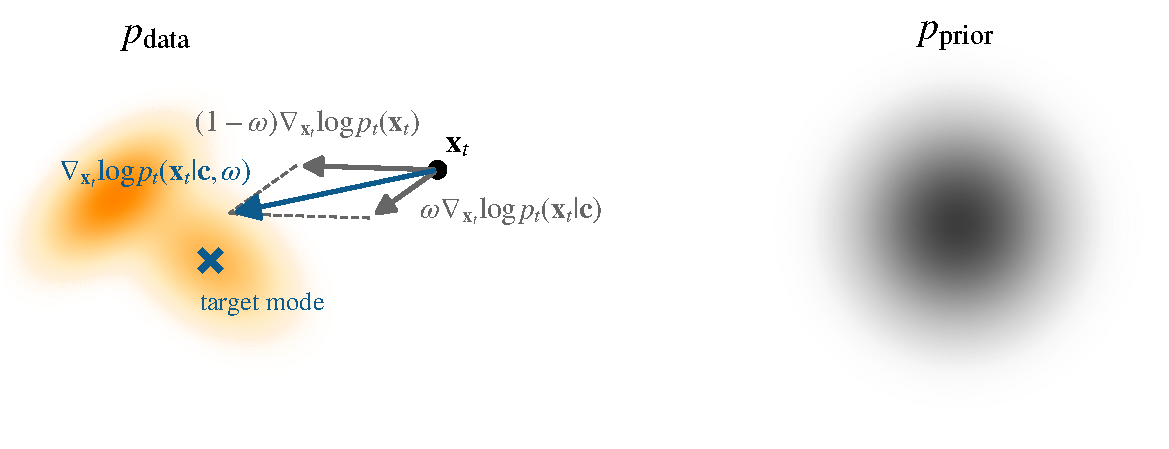
\includegraphics[width=\linewidth]{Images/PartB/classifier_guidance_v2.pdf}
    \caption{\textbfs{CFG 的示意图。} 调整后的分数 $\nabla_{\rvx_t} \log p_t(\rvx_t| \rvc, \omega)$ 由无条件分数 $\nabla_{\rvx_t} \log p_t(\rvx_t)$ 和条件分数 $\nabla_{\rvx_t} \log p_t(\rvx_t| \rvc)$ 之间的线性插值得到，并以 $\omega$ 为权重。所得方向将样本从先验引向与目标条件一致的数据分布模式。 \figcredit{由作者绘制。}}
    \label{fig:cfg}
\end{figure}

\emph{无分类器引导}（CFG）~\citep{ho2021classifier} 是基于分类器引导的一种简化方法，它消除了对独立分类器的需求。其核心思想是以一种无需显式分类器即可实现有效条件化的方式修改分数函数的梯度。具体而言，条件分布对数概率的梯度被调整为如下形式：
\begin{align}
    \nabla_{\rvx_t} \log p_t(\rvc | \rvx_t) = \nabla_{\rvx_t} \log p_t(\rvx_t | \rvc) - \nabla_{\rvx_t} \log p_t(\rvx_t).
\end{align}
将此表达式代入 \Cref{eq:cg_omega}，得到如下条件分数的公式：
\begin{align}\label{eq:cfg-model}
\nabla_{\rvx_t} \log p_t(\rvx_t | \rvc, \omega)
&= \nabla_{\rvx_t} \log p_t(\rvx_t) + \omega \left( \nabla_{\rvx_t} \log p_t(\rvx_t | \rvc) - \nabla_{\rvx_t} \log p_t(\rvx_t) \right) \nonumber\\
&= \omega \underbrace{\nabla_{\rvx_t} \log p_t(\rvx_t | \rvc)}_{\text{条件分数}} + (1 - \omega) \underbrace{\nabla_{\rvx_t} \log p_t(\rvx_t)}_{\text{无条件分数}}.
\end{align}

超参数 $\omega$ 再次在控制条件化信息影响方面发挥关键作用（我们取 $\omega \ge 0$）：
\begin{itemize}
    \item 当 $\omega = 0$ 时，模型表现为无条件扩散模型，完全忽略条件化信息。
    \item 当 $\omega = 1$ 时，模型使用条件分数，没有额外的引导。
    \item 当 $\omega > 1$ 时，模型更加强调条件分数而较少强调无条件分数，增强与 $\rvc$ 的对齐，但通常会降低多样性。
\end{itemize}

\subsection{CFG 的训练与采样}


\paragraph{通过 CFG 联合训练无条件与条件扩散模型。} 与 CG 不同，CFG 需要重新训练一个显式考虑条件变量 $\rvc$ 的扩散模型。然而，为条件和无条件分数函数分别训练两个独立模型通常在计算上不可行。为此，CFG 采用单个模型 $\mathbf{s}_{\bm{\phi}}(\rvx_t, t; \rvc)$，通过将 $\rvc$ 作为额外输入，在单个模型中同时学习两个分数函数。训练过程定义如下：
\begin{itemize}
    \item 对于无条件训练，传入空标记 $\emptyset$ 以替代条件化输入，得到 $\rvs_{\bm{\phi}}(\rvx_t, t, \emptyset)$。
    \item 对于条件训练，提供真实的条件变量 $\rvc$ 作为输入，得到 $\rvs_{\bm{\phi}}(\rvx_t, t, \rvc)$。
\end{itemize}
这两种训练机制通过以概率 $p_\mathrm{uncond}$（一个用户定义的超参数，通常设为 $0.1$）随机将 $\rvc$ 替换为空输入 $\emptyset$ 来统一。这种联合训练策略使模型能够同时学习条件和无条件分数函数。完整的训练算法见 \Cref{alg:cfg_training}，并与 \Cref{alg:no_cfg_training} 中所示的标准无条件训练进行了对比。我们注意到，在训练过程中并不使用 CFG 权重 $\omega$。

\begin{center}
\begin{minipage}[t]{0.48\textwidth}
  \begin{algorithm}[H]
  {\small
    {\small \caption{无条件扩散模型 \label{alg:no_cfg_training} }}
    \begin{algorithmic}[1]
      \Repeat
        \State $\rvx \sim p_{\text{data}}(\rvx)$
        \State $t \sim \mathcal{U}[0, T]$
        \State $\bm{\epsilon} \sim \mathcal{N}(\mathbf{0}, \mathbf{I})$
        \State $\rvx_t = \alpha_t \rvx + \sigma_t \bm{\epsilon}$
        \State 对以下式子进行梯度步：
        \Statex \quad $\nabla_{\bm{\phi}} \left\| \rvs_{\bm{\phi}}(\rvx_t, t) - \rvs \right\|^2$
      \Until{收敛}
    \end{algorithmic}
    }
  \end{algorithm}
\end{minipage}
\hfill
\begin{minipage}[t]{0.48\textwidth}
  \begin{algorithm}[H]
      {\small
    {\small \caption{用于条件扩散模型的 CFG \label{alg:cfg_training}}}
    \begin{algorithmic}[1]
      \Require \textcolor{orange}{$p_\mathrm{uncond}$：无条件 dropout 的概率}
      \Repeat
        \State \textcolor{orange}{$(\rvx, \rvc) \sim p_{\text{data}}(\rvx, \rvc)$}
        \State \textcolor{orange}{以概率 $p_\mathrm{uncond}$ 将 $\rvc \gets \emptyset$}
        \State $t \sim \mathcal{U}[0, T]$
        \State $\bm{\epsilon} \sim \mathcal{N}(\mathbf{0}, \mathbf{I})$
        \State $\rvx_t = \alpha_t \rvx + \sigma_t \bm{\epsilon}$
        \State 对以下式子进行梯度步：
        \Statex \quad \textcolor{orange}{$\nabla_{\bm{\phi}} \left\| \rvs_{\bm{\phi}}(\rvx_t, t, \rvc) - \rvs \right\|^2$}
      \Until{收敛}
    \end{algorithmic}
    }
  \end{algorithm}
\end{minipage}
\end{center}

\paragraph{使用 CFG 进行条件采样。}

一旦使用算法~\ref{alg:cfg_training} 训练了模型 $\rvs_{\bm{\phi}^\times}(\rvx_t, t, \rvc)$，就可以在采样时应用 CFG。对数概率的梯度由下式给出：
\begin{align}\label{eq:cfg-model-nn}
\nabla_{\rvx_t} \log p_t(\rvx_t | \rvc, \omega)
&= \omega \nabla_{\rvx_t} \log p_t(\rvx_t | \rvc) + (1 - \omega) \nabla_{\rvx_t} \log p_t(\rvx_t) \nonumber\\
&\approx \omega \underbrace{\rvs_{\bm{\phi}^\times}(\rvx_t, t, \rvc)}_{\text{条件分数}} + (1 - \omega) \underbrace{\rvs_{\bm{\phi}^\times}(\rvx_t, t, \emptyset)}_{\text{无条件分数}}\\
&=: \rvs_{\bm{\phi}^\times}^{\text{CFG}}(\rvx_t ,t, \rvc; \omega). \nonumber
\end{align}

在采样过程中，应用固定的（或可选地随时间变化的）无分类器引导权重 $\omega$。然后，逆向时间 SDE（\Cref{eq:sde_backward}）或 PF-ODE（\Cref{eq:fp_general}）中的无条件分数 $\nabla_{\rvx_t} \log p_t(\rvx_t)$ 被引导分数 $\rvs_{\bm{\phi}^\times}^{\mathrm{CFG}}(\rvx_t ,t, \rvc; \omega)$ 替换（如 \Cref{eq:condition_prob_ode} 所示），它以加权方式结合了条件分数和无条件分数。

这一公式通过调整 $\omega$ 实现了可控生成，使样本能够在保持多样性的同时被引向条件化信号 $\rvc$。因此，CFG 提供了一种有效且计算高效的方式来实现精确的条件生成，因为它只需训练单个扩散模型。

% \msg{Score Decomposition via Bayes' Rule for Guided Generation}{A key idea behind both CG and CFG is the decomposition of the conditional score into two parts: an unconditional term and a guidance term. This identity follows directly from Bayes' rule (see \Cref{eq:cg_bayes}) and provides a general way to guide diffusion models using auxiliary information. We restate this important formula below, where $\rvy$ denotes the additional information:
% \begin{mdframed}
%     \begin{align}
% \nabla_{\rvx_t} \log p(\rvx_t | \rvy) = \underbrace{\nabla_{\rvx_t} \log p_t(\rvx_t)}_{\text{uncond. direction}}
% + \underbrace{\nabla_{\rvx_t} \log p_t(\rvy | \rvx_t)}_{\text{guidance direction}}. \label{eq:guidance_bayes}
% \end{align}
% \end{mdframed}

% This decomposition makes it possible to use diffusion models in many ways by approximating the guidance term $\nabla_{\rvx_t} \log p_t(\rvy | \rvx_t)$ based on the application. For example, it enables controllable generation by steering samples toward desired attributes $\rvy$, solves inverse problems at test time using observed measurements, and allows one trained model to handle different tasks by applying suitable guidance signals.


% }

\clearpage
\newpage






\section{免训练引导}
本节介绍支撑一大类免训练引导方法~\citep{chung2023diffusion,ye2024tfg,he2024manifold,bansal2023universal} 的高层哲学。尽管在实现和应用上各有差异，这些方法都统一于 \Cref{eq:guidance_bayes} 所表达的核心原则。我们首先在 \Cref{subsec:tfg} 中介绍免训练引导的高层方法，然后将这一思想扩展到免训练的逆问题求解，并在 \Cref{subsec:inverse-problem} 中给出简要概述。


\paragraph{设置与符号。} 设 $\rvc$ 表示条件变量。我们假设可以访问以分数预测表示的预训练扩散模型 $\rvs_{\bm{\phi}^\times}(\rvx_t, t)$\footnote{为简化数学表达，这里我们采用分数和 $\rvx$-预测参数化；其他参数化（例如 $\beps$-预测）可类似处理。}。此外，假设给定一个非负函数
\[
\ell(\cdot, \rvc) \colon \mathbb{R}^D \to \mathbb{R}_{\geq 0}
\]
用于量化样本 $\rvx \in \mathbb{R}^D$ 与条件 $\rvc$ 的对齐程度，其中 $\ell(\rvx, \rvc)$ 的值越小表示对齐越强。此类函数的具体示例包括：(i) $\rvc$ 是参考图像，$\ell(\cdot, \rvc)$ 是度量感知接近度的相似度得分；(ii) $\ell(\cdot, \rvc)$ 是通过预训练模型（例如 CLIP~\citep{radford2021learning}）计算的基于特征的相似度得分。


考虑标准的线性—高斯前向加噪核
 $p_{t}(\cdot| \rvx_0):=\mathcal{N}\big(\cdot; \alpha_t\rvx_0, \sigma^2_t\mathbf{I}\big)$。
我们回顾 \Cref{eq:ddim-update-all} 中的 DDIM 更新，并以它为例：
\begin{align}\label{eq:ddim-update-clean-noise-score}
\begin{aligned}
    \rvx_{t \rightarrow t-1} =\alpha_{t-1} \underbrace{\hat{\rvx}_0(\rvx_t)}_{\text{在数据空间}} - \sigma_{t-1} \sigma_t \underbrace{\hat{\rvs}(\rvx_t)}_{\text{在噪声空间}},
\end{aligned}
\end{align}
其中 $\hat{\rvx}_0(\rvx_t):=\rvx_{\bm{\phi}^\times}(\rvx_t, t)$ 是（干净的）$\rvx$-预测，$\hat{\rvs}(\rvx_t):=\rvs_{\bm{\phi}^\times}(\rvx_t, t)$ 是在时刻水平 $t$ 从 $\rvx_t$ 出发的分数预测。

\subsection{免训练引导的概念框架}\label{subsec:tfg}
大多数免训练引导方法~\citep{ye2024tfg} 在\emph{数据空间}或\emph{噪声空间}中引入校正，以将 \Cref{eq:ddim-update-clean-noise-guide} 中的 DDIM 更新引向满足条件 $\rvc$：
\begin{align}\label{eq:ddim-update-clean-noise-guide}
\begin{aligned}
    \rvx_{t \rightarrow t-1} &=\alpha_{t-1} \underbrace{\left(\hat{\rvx}_0(\rvx_t) + {\color{orange}\eta_t^{\text{data}}\mathcal{G}_0} \right)}_{\text{A. 数据空间}}
    - \sigma_{t-1} \sigma_t \underbrace{\left(\hat{\rvs}(\rvx_t) + {\color{orange}\eta_t^{\text{latent}}\mathcal{G}_t} \right)}_{\text{B. 噪声空间}},
\end{aligned}
\end{align}
其中 $\eta_t^{\text{data}}, \eta_t^{\text{latent}} \geq 0$ 是随时间变化的引导强度，$\mathcal{G}_0$、$\mathcal{G}_t$ 是下面定义的校正项。

\paragraph{A. 数据空间中的引导。}
沿负梯度方向下降
\[
\mathcal{G}_0 := -\nabla_{\rvx_0} \ell(\rvx_0, \rvc),
\]
修改后数据空间中的干净估计
\[
\hat{\rvx}_0(\rvx_t) + {\color{orange}\eta_t^{\text{data}} \mathcal{G}_0},
\]
可以逐步被引向更好地满足条件 $\rvc$ 的样本。这种梯度下降方案可以迭代地应用，以渐进地改善对齐。

代表性示例包括 MGPD~\citep{he2023manifold} 和 UGD~\citep{bansal2023universal}。


% This strategy can also be interpreted as the conditional score decomposition \Cref{eq:guidance_bayes}.

% \begin{align*}
% \nabla_{\rvx_t} \log p_t(\rvx_t|\rvc)
% &= \underbrace{\nabla_{\rvx_t} \log p_t(\rvx_t)}_{\text{unconditional}}
% + \underbrace{\nabla_{\rvx_t} \log p(\rvc|\rvx_t)}_{\text{guidance}}
% \\&\approx \rvs_{\bm{\phi}^\times}(\rvx_t,t) + \eta_t^{\text{latent}} \mathcal{G}_t,
% \end{align*}
% \[
% p(\rvc|\rvx_0) \propto \ell(\rvx_0, \rvc),
% \]
% viewing $\ell_\rvc$ as a surrogate likelihood on the clean signal.

\paragraph{B. 噪声空间中的引导。}
如 \Cref{sec:prologue-guidance} 所讨论，条件分数 $\nabla_{\rvx_t} \log p_t(\rvc|\rvx_t)$ 通常难以处理。一种实用的近似是引入一个替代似然 $\widetilde p_t(\mathbf{c}|\mathbf{x}_t)$：
\[
\widetilde p_t(\mathbf{c}|\mathbf{x}_t) \propto \exp \big(-\eta\ell \left(\hat{\rvx}_0(\rvx_t), \rvc\right)\big)
\]
带有一个重缩放常数 $\eta>0$，使得
\[
\nabla_{\rvx_t}\log \widetilde p_t(\mathbf{c}|\mathbf{x}_t) = -\eta\nabla_{\rvx_t}\ell \left(\hat{\rvx}_0(\rvx_t), \rvc\right) =: \mathcal{G}_t,
\]
其中 $\hat{\rvx}_0(\rvx_t)$ 通过扩散模型的预测得到。
% Then, the guidance direction becomes
% \[
% \nabla_{\rvx_t} \log p_t(\rvc | \rvx_t)
% \approx \nabla_{\rvx_t} \log \ell_\rvc\left(\hat{\rvx}_0(\rvx_t)\right)
% =:\mathcal{G}_t.
% \]
将其代入条件分数的贝叶斯公式，得到代理：
\begin{align*}
\nabla_{\rvx_t} \log p_t(\rvx_t|\rvc)
&\approx \underbrace{\nabla_{\rvx_t} \log p_t(\rvx_t)}_{\text{无条件}}
+ \underbrace{\nabla_{\rvx_t} \log \widetilde p_t(\mathbf{c}|\mathbf{x}_t)}_{\text{引导}}
\\&\approx \hat{\rvs}(\rvx_t) + \eta_t^{\text{latent}} \mathcal{G}_t,
\end{align*}
它充当噪声空间中的引导校正项。


然而，我们注意到计算 $\mathcal{G}_t$ 需要通过 $\rvx$-预测进行反向传播，即
\[
\nabla_{\rvx_t} \hat{\rvx}_0(\rvx_t)^\top \cdot
\left.\nabla_{\rvx_0} \log \ell_{\rvc}(\rvx_0)\right|_{\rvx_0 = \hat{\rvx}_0(\rvx_t)},
\]
这在实践中可能带来相当大的计算开销。

代表性示例包括 \citep{yu2023freedom, chung2022diffusion, bansal2023universal}.




\subsection{免训练方法求解逆问题的示例}\label{subsec:inverse-problem}
\Cref{subsec:tfg} 中介绍的原则在逆问题中有重要的应用。我们先概述背景，然后给出若干具体示例，说明如何利用预训练的扩散模型在推理时求解逆问题。

\paragraph{逆问题的背景。}
设 $\mathcal{A}$ 为退化算子（可以是线性或非线性的，已知或未知的），例如模糊核或图像修复算子，$\mathbf{y}$ 是由如下退化模型生成的观测：
\begin{align}\label{eq:inverse_problem}
    \mathbf{y} = \mathcal{A}(\mathbf{x}_0) + \sigma_{\mathbf{y}} \mathbf{z}, \quad \mathbf{z} \sim \mathcal{N}(\mathbf{0}, \mathbf{I}).
\end{align}
逆问题的目标是从后验分布 $p_0(\mathbf{x}_0 | \mathbf{y})$ 中采样，其中对于给定的观测 $\mathbf{y}$，可能存在无穷多个可能的重建 $\mathbf{x}_0$。目标是恢复一个去除 $\mathbf{y}$ 中退化同时保留其忠实和语义特征的 $\mathbf{x}_0$。


求解逆问题的传统方法通常遵循有监督的框架，需要收集退化样本与恢复样本的成对数据 $(\mathbf{y}, \mathbf{x})$，并依赖优化方法或神经网络的有监督训练。这类方法在数据准备上成本高昂，且对未见数据的泛化能力可能不足。


\paragraph{将预训练扩散模型用作逆问题求解器。}
如前所述，条件分数可以通过贝叶斯法则分解：
\begin{align}
 \nabla_{\rvx_t} \log p_t(\rvx_t | \rvy) = \underbrace{\nabla_{\rvx_t} \log p_t(\rvx_t)}_{\text{数据分数}} + \underbrace{\nabla_{\rvx_t}\log p_t(\rvy | \rvx_t)}_{\text{观测对齐}}.
\label{eq:bayes_rule}
\end{align}

这一分解将数据分数与一个逆问题特有的与 $\rvy$ 的观测对齐项分开。它使我们可以通过对干净数据分布 $ p_{\text{data}} $ 建模并在反演过程中加以应用，从而以无监督方式求解 \Cref{eq:inverse_problem}。更具体地：
\begin{itemize}
    \item \textbfs{数据分数 $\nabla_{\rvx_t} \log p_t(\rvx_t)$：} 使用在干净数据上训练的预训练扩散模型 $\rvs_{\bm{\phi}^\times}(\rvx_t, t)$ 来近似。
    \item \textbfs{观测对齐 $\nabla_{\rvx_t} \log p_t(\rvy | \rvx_t)$：} 没有闭式形式，因为它涉及对隐变量的边缘化。
\end{itemize}

因此，使用预训练扩散模型的大多数免训练方法都聚焦于近似 $\nabla_{\rvx_t} \log p_t(\rvy | \rvx_t)$。我们采用 \citep{daras2024survey} 中总结的一种通用元形式：
\begin{equation*}
    \nabla_{\rvx_t} \log p_t(\rvy | \rvx_t) \approx - \frac{\eqnmarkbox[Plum]{proj}{\mathcal{P}_t}  \, \eqnmarkbox[NavyBlue]{merror}{    \mathcal{M}_t    }}{\eqnmarkbox[OliveGreen]{guidance}{  \gamma_t  }}.
\end{equation*}
其中：
\begin{itemize}
    \item $\mathcal{M}_t$：量化观测 $\rvy$ 与估计信号之间失配的误差向量，
    \item $\mathcal{P}_t$：将 $\mathcal{M}_t$ 投影回 $\rvx_t$ 所处空间的映射，
    \item $\gamma_t$：控制引导强度的标量。
\end{itemize}

代表性方法对 $\mathcal{M}_t$、$\mathcal{P}_t$ 和 $\gamma_t$ 的实例化各不相同，下面以带颜色标注的组件加以说明。

\paragraph{基于扩散模型的逆问题求解器的实例化。}
我们介绍一些代表性方法，它们利用预训练的扩散模型提供无监督方法（无需成对数据），可灵活应用于各种逆问题，且使用同一个学习得到的 $ p_{\mathrm{data}} $ 代理。


\subparagraph{Score SDE~\citep{song2020score}。} 最早基于扩散模型的逆问题求解器之一。它考虑已知的线性退化模型 $\rmA$，并聚焦于 $\sigma_{\rvy} = 0$ 的无噪声设定。由于 $\rmA$ 是线性的，可以构造噪声水平匹配的观测
\[
\rvy_t := \alpha_t \rvy + \sigma_t \bm{\epsilon},
\]
并利用残差 $\rvy_t - \rmA \rvx_t$（注意：一般而言 $\rvy_t \neq \rmA\rvx_t$）驱动一种似然式的校正。一种常见的近似（舍去乘性常数）是
\begin{align*}
    \nabla_{\rvx_t} \log p_t(\rvy|\rvx_t) \approx - \eqnmarkbox[Plum]{proj}{\rmA^\top} (\eqnmarkbox[NavyBlue]{noisymeasurements}{\rvy_t - \rmA \rvx_t}).
\end{align*}

\subparagraph{迭代隐变量细化（ILVR）~\citep{choi2021ilvr}。} 使用与 ScoreSDE 相同的设定，ILVR 估计：
\begin{align*}
    \nabla_{\rvx_t} \log p_t(\rvy| \rvx_t) \approx -\rmA^\dagger(\rvy_t - \rmA\rvx_t) = -\eqnmarkbox[Plum]{moore}{(\rmA^\top \rmA)^{-1} \rmA^\top} (\eqnmarkbox[NavyBlue]{merror}{\rvy_t - \rmA\rvx_t}),
\end{align*}
其中 $\rmA^\dagger$ 是 Moore–Penrose 伪逆，$\rvy_t = \alpha_t\rvy + \sigma_t \bm{\epsilon}_t$。
\subparagraph{扩散后验采样（DPS）~\citep{chung2022diffusion}。} 一种针对已知非线性前向算子 $\mathcal{A}$ 和加性高斯噪声水平 $\sigma_{\rvy} \ge 0$ 的逆问题被广泛使用的方法是\emph{去噪后验分数}（DPS），它近似
\begin{align}\label{eq:dps-score}
  \nabla_{\rvx_t} \log p_t(\rvy|\rvx_t)
   \approx
  \nabla_{\rvx_t} \log p_t\bigl(\rvy|X_0 = \hat\rvx_0(\rvx_t)\bigr),
\end{align}
其中 $\hat\rvx_0(\rvx_t) := \E[\rvx_0|\rvx_t]$ 表示在时刻 $t$ 给定带噪观测 $\rvx_t$ 时干净样本的条件均值，通常用预训练扩散模型通过 Tweedie 公式（\Cref{eq:tweedie}）估计。

这一单点近似假设条件分布 $p(\rvx_0|\rvx_t)$ 高度集中，它源自：
\begin{align*}
  p_t(\rvy|\rvx_t)
  &= \int p_t(\rvy|\rvx_t, \rvx_0)  p(\rvx_0|\rvx_t)  \mathrm{d}\rvx_0 \\
  &= \int p_t(\rvy|\rvx_0)  p(\rvx_0|\rvx_t)  \mathrm{d}\rvx_0
   \approx  p_t\bigl(\rvy|X_0=\hat\rvx_0(\rvx_t)\bigr),
\end{align*}
其中我们利用了在给定 $\rvx_0$ 时 $\rvy$ 仅依赖于 $\rvx_0$（不依赖于 $\rvx_t$）这一事实，且近似在后验 $p(\rvx_0|\rvx_t)$ 紧密集中于其均值的假设下成立。

由于
\[
  p_t\bigl(\rvy|X_0 = \hat\rvx_0(\rvx_t)\bigr)
  = \mathcal{N}\bigl(\rvy;  \mathcal{A}(\hat\rvx_0(\rvx_t)),  \sigma_{\rvy}^2 \rmI\bigr),
\]
我们计算
\begin{align*}
  \nabla_{\rvx_t} \log p_t(\rvy|\rvx_t)
  &\approx \nabla_{\rvx_t} \log \mathcal{N}\bigl(\rvy;  \mathcal{A}(\hat\rvx_0),  \sigma_{\rvy}^2 \rmI\bigr) \\
  &= -\frac{1}{2\sigma_{\rvy}^2}  \nabla_{\rvx_t} \bigl\| \rvy - \mathcal{A}(\hat\rvx_0) \bigr\|^2 \quad  \\
  &= \frac{1}{\sigma_{\rvy}^2}  \left[ \mathcal{J}_{\mathcal{A}}\big(\hat\rvx_0(\rvx_t)\big) \cdot \nabla_{\rvx_t} \hat\rvx_0(\rvx_t) \right]^\top \bigl( \rvy - \mathcal{A}\big(\hat\rvx_0(\rvx_t)\big) \bigr),
\end{align*}
其中 $\mathcal{J}_{\mathcal{A}}\big(\hat\rvx_0(\rvx_t)\big) := \nabla_{\rvx_0} \mathcal{A}(\rvx) \big|_{\rvx = \hat\rvx_0(\rvx_t)}$ 表示前向算子关于其输入的雅可比矩阵。这一公式将梯度通过分数近似流程传播，反映了测量似然如何随带噪样本 $\rvx_t$ 的扰动而变化。

对于线性逆问题，这进一步简化为：
\begin{align*}
    \nabla_{\rvx_t} \log p_t(\rvy | \rvx_t) \approx \eqnmarkbox[OliveGreen]{guidance}{\frac{1}{\sigma_{\rvy}^2}}  \,  \eqnmarkbox[Plum]{proj}{\left[ \rmA \cdot \nabla_{\rvx_t} \hat\rvx_0(\rvx_t) \right]^\top} \left(\eqnmarkbox[NavyBlue]{merror}{\rvy - \rmA(\hat\rvx_0(\rvx_t))}\right).
\end{align*}

大量工作通过为 $\nabla_{\rvx_t} \log p_t(\rvy | \rvx_t)$ 提出各种近似来探索基于扩散模型的逆问题求解器。如需全面综述，读者可参阅 \citet{daras2024survey} 的综述。



\paragraph{一个相关的有监督迭代恢复视角及其与 PF-ODE 的联系。}
上面的讨论通过将预训练扩散先验与 \Cref{eq:bayes_rule} 中的贝叶斯法则分解相结合来求解逆问题。更具体地，这些方法使用先验分布的分数结合测量模型来引导重建过程。同时，它们也反映了一个更广泛的思想：与其一步恢复干净信号，不如通过许多小的更新逐步改进一个退化的输入。类似的高层策略也出现在有监督的图像恢复中，但出发点不同。这些方法不使用预训练的分数模型作为先验，而是直接从成对的退化和干净样本中学习细化过程。

一个代表性示例是 InDI~\citep{delbracio2023inversion}。与上面基于贝叶斯法则的方法不同，InDI 从成对数据 $(\rvy,\rvx_0)$ 出发，其中 $\rvy$ 是退化观测，$\rvx_0$ 是对应的干净目标。重要的是，它一般不假设从 $\rvx_0$ 到 $\rvy$ 的退化过程是解析已知的，也不假设它是高斯的。

其基本思想是通过插值路径连接两个端点
\[
\rvx_t=(1-t)\rvx_0+t\rvy,\qquad t\in[0,1].
\]
这条路径应仅被理解为从干净目标到退化观测的一条方便轨迹。它一般不是高斯加噪过程。沿此路径，对于任意 $0\le s\le t$，有精确关系
\[
\rvx_s=\Bigl(1-\frac{s}{t}\Bigr)\rvx_0+\frac{s}{t}\rvx_t.
\]
对 $\rvx_t$ 取条件期望得到
\[
\mathbb E[\rvx_s|\rvx_t]
=
\Bigl(1-\frac{s}{t}\Bigr)\mathbb E[\rvx_0|\rvx_t]
+
\frac{s}{t}\rvx_t.
\]
这表明，要从当前状态 $\rvx_t$ 移动到一个略微不那么退化的状态，只需从 $\rvx_t$ 预测干净目标即可。

基于这一思想，人们从成对样本中通过最小化回归目标训练一个时间条件预测器 $\rmF_{\bphi}(\rvx_t,t)$
\[
\min_{\bphi}\;
\mathbb E_{(\rvx_0,\rvy)\sim p(\rvx_0,\rvy),\, t\sim p(t)}
\Bigl\|
\rmF_{\bphi}\bigl((1-t)\rvx_0+t\rvy,\,t\bigr)-\rvx_0
\Bigr\|_2^2,
\]
其中 $p(\rvx_0,\rvy)$ 表示由干净目标 $\rvx_0$ 及其退化观测 $\rvy$ 组成的数据对的联合分布，$p(t)$ 指定训练时插值时间如何采样。
也就是说，$\rmF_{\bphi}$ 被训练为从沿插值路径的中间退化状态预测干净目标。对于这一平方误差损失，贝叶斯最优预测器是条件期望
\[
\rmF^*(\rvx_t,t)=\mathbb E[\rvx_0|\rvx_t].
\]
因此，如果模型类足够有表达力且优化成功，学习得到的预测器近似于时刻 $t$ 与中间状态 $\rvx_t$ 关联的平均干净目标。在这个意义上，训练目标在精神上类似于扩散模型的训练：两者都是学习一个从中间退化状态到更干净目标的时间条件回归。区别在于扩散模型从规定的前向退化过程中合成地生成这样的训练对，而这里的端点对 $(\rvy,\rvx_0)$ 直接来自有监督的恢复数据。

在推理时，从 $\hat{\rvx}_1=\rvy$ 开始，反复通过下式细化估计
\[
\hat{\rvx}_{t-\Delta t}
=
\frac{\Delta t}{t}\rmF_{\bphi}(\hat{\rvx}_t,t)
+
\Bigl(1-\frac{\Delta t}{t}\Bigr)\hat{\rvx}_t.
\]
因此，最终重建是由逐步细化而非单次直接预测产生的。在连续时间极限下，这导出 InDI 的残差流 ODE
\[
\frac{\diff \rvx_t}{\diff t}
=
\frac{\rvx_t-\rmF_{\bphi}(\rvx_t,t)}{t}.
\]

现在假设我们进一步特化到高斯去噪设定，即假设退化取已知的解析形式
\[
\rvy=\rvx_0+\sigma\beps,
\qquad \beps\sim\mathcal N(\bm 0,\rmI),
\]
噪声水平 \(\sigma\) 已知。在这一特化下，InDI 的残差流 ODE 恰好退化为概率流 ODE。事实上，插值路径变为
\[
\rvx_t=(1-t)\rvx_0+t\rvy
=
\rvx_0+t\sigma\beps,
\]
这正是标准扩散形式
\[
\rvx_t=\alpha_t\rvx_0+\sigma_t\beps,
\qquad\text{其中}\qquad
\alpha_t=1,\;\sigma_t=t\sigma.
\]
因此，预测器 \(\rmF_{\bphi}(\rvx_t,t)\approx \mathbb E[\rvx_0\mid \rvx_t]\) 现在学习的是对高斯退化的中间状态 \(\rvx_t\) 进行去噪。此时，残差流 ODE 变为
\[
\frac{\diff \rvx_t}{\diff t}
=
\frac{\rvx_t-\mathbb E[\rvx_0\mid \rvx_t]}{t}
=
-\dot{\sigma}_t\sigma_t\nabla_{\rvx_t}\log p_t(\rvx_t),
\]
其中最后一个等式由 \(\sigma_t=t\sigma\) 以及 Tweedie 公式得到，
\[
\mathbb E[\rvx_0\mid \rvx_t]
=
\rvx_t+\sigma_t^2\nabla_{\rvx_t}\log p_t(\rvx_t).
\]
这正是该高斯去噪路径的 PF-ODE，写成去噪器形式或分数形式。因此，在高斯去噪特化下，InDI 给出了扩散建模的另一种解释：可以将其视为在高斯退化数据上的有监督去噪器学习，而 PF-ODE 作为逐步细化的连续时间极限出现。



\newpage
\section{从强化学习到用于模型对齐的直接偏好优化}\label{sec:rlhf-dpo}

% In the pursuit of aligning generative models with human intent, the prevailing paradigm has been Reinforcement Learning from Human Feedback (RLHF). While effective, RLHF is a complex, multi-stage process prone to instability. This section introduces \emph{Direct Preference Optimization (DPO)}, a more streamlined and stable method that achieves the same objective without the need for explicit reward modeling or reinforcement learning. We then explore its extension to a different generative class with \emph{Diffusion-DPO}.

% \subsection{The Motivation: Circumventing the Pitfalls of RLHF}

% The goal of alignment is to steer a base, pre-trained model (such as a supervised fine-tuned LLM) to produce outputs that humans prefer. The RLHF framework tackles this in three distinct stages. First, supervised fine-tuning (SFT) trains a base model on a dataset of prompt-response pairs. Second, reward modeling (RM) trains a separate model on human preferences consisting of prompts $\mathbf{c}$ and paired responses, one preferred ($\mathbf{x}_w$, ``winner'') and one dispreferred ($\mathbf{x}_l$, ``loser''), with the reward model $r(\mathbf{c},\mathbf{x})$ assigning higher scalar reward to the winner. Finally, RL fine-tuning optimizes the SFT model (now a policy $\pi$) using an RL algorithm such as PPO, maximizing reward-model scores while being regularized by a KL-divergence penalty that keeps $\pi$ close to the reference distribution.

% Despite its impact, this pipeline suffers from drawbacks: the RL stage is unstable and computationally expensive, involving repeated sampling from the policy; it requires training and hosting multiple large models (SFT, reward, and possibly value models); and it optimizes only a proxy for human preferences, meaning flaws in the reward model can be exploited. This motivates a central question:
% \begin{question}
%     Can we eliminate explicit reward modeling and the unstable RL process, directly optimizing the model on preference data?
% \end{question}
在追求将生成式模型与人类意图对齐的过程中，主流范式一直是基于人类反馈的强化学习（RLHF）。尽管有效，RLHF 是一个复杂、多阶段且可能不稳定的过程。本节介绍\emph{直接偏好优化（DPO）}~\citep{rafailov2023direct}，它是一种更精简且稳定的方法，无需显式奖励建模或强化学习即可达到同样的目标。随后我们概述它通过 \emph{Diffusion-DPO}~\citep{wallace2024diffusion} 向扩散模型的扩展。

\subsection{动机：规避 RLHF 的陷阱}

对齐的目标是将一个基础的预训练模型（例如 SFT 模型）引导向人类偏好的输出。RLHF 分三个阶段进行。首先，\emph{有监督微调（SFT）}在提示—响应对上训练一个基础模型。其次，\emph{奖励建模（RM）}在偏好数据上拟合一个模型，该数据由提示 $\mathbf{c}$ 和成对的响应（一个偏好的"赢家" $\mathbf{x}_w$ 和一个不偏好的"输家" $\mathbf{x}_l$）组成，学习一个标量 $r(\mathbf{c},\mathbf{x})$ 使得 $r(\mathbf{c},\mathbf{x}_w)>r(\mathbf{c},\mathbf{x}_l)$。第三，\emph{RL 微调}用诸如 PPO~\citep{schulman2017proximal} 之类的算法优化 SFT 模型（策略 $\pi$\footnote{策略将一个提示/历史（状态）映射到响应/动作上的分布。}），最大化来自 $r$ 的期望奖励，同时通过 KL 惩罚进行正则化，使 $\pi$ 保持在参考/SFT 分布附近。

尽管影响深远，这一流程存在缺陷：RL 阶段不稳定且计算昂贵，因为它是同策略的——每次更新都需要从当前模型新鲜生成的样本；它还需要训练和部署多个大型模型（SFT、奖励，有时还有价值模型）；而且它只优化人类偏好的代理，因此奖励模型中的缺陷可能被利用。这引出一个核心问题：
\begin{question}
    我们能否消除显式的奖励建模和不稳定的 RL 步骤，直接在偏好数据上优化模型？
\end{question}

直接偏好优化（DPO）通过用单个、有监督式的步骤替代多阶段的 RLHF 流程来简化对齐。DPO 不再训练一个单独的奖励模型并运行像 PPO 这样不稳定的 RL 算法，而是直接用一个简单的逻辑损失将策略拟合到偏好对上，同时保持接近一个固定的参考模型。其关键洞察是，KL 正则化的 RLHF 目标可以被改写，使得策略与参考之间的对数似然比充当一个隐式奖励。这保留了对参考策略的相同正则化，但避免了昂贵的采样回放和显式奖励建模。

在 \Cref{subsec:rlhf-bradley-terry} 中，我们简要回顾 RLHF 流程及其对大型奖励模型和 RL 微调的依赖。在 \Cref{subsec:dpo} 中，我们介绍最初为语言模型提出的 DPO，它规避了奖励模型训练并简化了对齐微调。最后，在 \Cref{subsec:diffusion-dpo} 中，我们将这一思想扩展到扩散模型，把 Diffusion-DPO 作为生成式建模场景中一种实用且稳定的对齐方法加以介绍。

\subsection{RLHF：Bradley--Terry 视角}\label{subsec:rlhf-bradley-terry}


\paragraph{RLHF 简要介绍。}
RLHF 从一个学习得到的评判者开始：一个奖励模型 $r_{\bm\psi}$，它为同一提示 $\mathbf c$ 的候选响应赋予标量偏好分数。数据集 $\mathcal D$ 由成对的 $(\tilde{\mathbf x},\mathbf x)$ 组成，并标注了标签 $y$，指示 $\tilde{\mathbf x}$ 是否优于 $\mathbf x$。标签可以是二值的 $y\in\{0,1\}$，也可以是通过汇总多个评分者得到的软值 $y\in[0,1]$。训练目标是一个简单的逻辑损失
\begin{align}\label{eq:rm-emp}
\begin{aligned}
    \mathcal L_{\mathrm{RM}}(\bm\psi)
=
- \mathbb E_{(\mathbf c,\tilde{\mathbf x},\mathbf x,y)\sim\mathcal D}
\Big[
y &\log \sigma \big(r_{\bm\psi}(\mathbf c,\tilde{\mathbf x})-r_{\bm\psi}(\mathbf c,\mathbf x)\big)
\\ &+(1-y)\log \big(1-\sigma \big(r_{\bm\psi}(\mathbf c,\tilde{\mathbf x})-r_{\bm\psi}(\mathbf c,\mathbf x)\big)\big)
\Big],
\end{aligned}
\end{align}
其中 $\sigma(u)=1/(1+e^{-u})$。在实践中，$\mathcal D$ 中的偏好对可能来自多种来源：精选的响应、不同检查点处的模型快照，或预训练条件扩散模型的生成结果。
一种标准约定是以有序格式 $(\text{赢家}, \text{输家})$ 存储它们。
在这一约定下，我们简单地设 $y=1$，\Cref{eq:rm-emp} 退化为特例（令 $\tilde\rvx = \rvx^w$ 且 $\rvx = \rvx^l$）：
\begin{equation}\label{eq:rm-bt}
\mathcal L_{\mathrm{RM}}(\bm\psi)
=
- \mathbb E_{(\mathbf c,\mathbf x_w,\mathbf x_l)\sim\mathcal D}
\Big[\log \sigma \big(r_{\bm\psi}(\mathbf c,\mathbf x_w)-r_{\bm\psi}(\mathbf c,\mathbf x_l)\big)\Big].
\end{equation}


\paragraph{Bradley--Terry 视角与 KL 联系。}
通常通过 Bradley--Terry（BT）模型~\citep{bradley1952rank} 来解释
\[
p_{r_{\bm\psi}}(\tilde{\mathbf x}\succ \mathbf x|\mathbf c)
 := \sigma \big(r_{\bm\psi}(\mathbf c,\tilde{\mathbf x})-r_{\bm\psi}(\mathbf c,\mathbf x)\big)
\]
该模型将两个标量分数转换为获胜概率。
这一表述突出了两个关键性质：(i) 只有分数的\emph{差}才重要（因此 $r_{\bm\psi}(\mathbf c,\cdot)$ 是平移不变的），(ii) 损失推动预测赢家的分数高于输家的分数。为了直观理解 (ii)，考虑一个标签为 $y\in\{0,1\}$ 的对，并定义
\[
\Delta r := r_{\bm\psi}(\mathbf c,\tilde{\mathbf x})-r_{\bm\psi}(\mathbf c,\mathbf x),
\quad
p:=\sigma(\Delta r),\quad \sigma(u)=\tfrac{1}{1+e^{-u}}.
\]
单样本的逻辑损失是
\[
\ell=-\big[y\log p+(1-y)\log(1-p)\big].
\]
那么
\[
\frac{\partial \ell}{\partial \Delta r}=\sigma(\Delta r)-y.
\]
在步长 $\eta>0$ 的梯度下降下，分数差的更新为
\[
\Delta r \leftarrow \Delta r-\eta\big(\sigma(\Delta r)-y\big).
\]
因此，如果 $y=1$（"$\tilde{\mathbf x}$ 获胜"），则 $\sigma(\Delta r)-1\le 0$，所以 $\Delta r$ 增大（赢家升、输家降）；如果 $y=0$，则 $\Delta r$ 减小。


\Cref{eq:rm-emp} 中的每个单样本项可以视为观测到的伯努利标签与模型预测的获胜概率之间的交叉熵：
\[
-\big[y\log p_{r_{\bm\psi}}+(1-y)\log(1-p_{r_{\bm\psi}})\big]
= \mathcal D_{\mathrm{KL}} \big(\mathrm{Bern}(y) \big\| \mathrm{Bern}(p_{r_{\bm\psi}})\big)
+ \mathcal H \big(\mathrm{Bern}(y)\big),
\]
其中 $\mathcal H$ 是目标伯努利分布的熵。
在数据集 $\mathcal D$ 上平均得到
\begin{align}\label{eq:reward_loss}
    \mathcal L_{\mathrm{RM}}(\bm\psi)
= \mathbb E_{\mathcal D} \Big[\mathcal D_{\mathrm{KL}}\left(\mathrm{Bern}(y) \big\| \mathrm{Bern}(p_{r_{\bm\psi}})\right)\Big]
+ \underbrace{\mathbb E_{\mathcal D} \big[\mathcal H(\mathrm{Bern}(y))\big]}_{\text{与 }\bm\psi 无关}.
\end{align}
因此，最小化逻辑损失等价于最小化人类标签的经验伯努利分布与模型预测的伯努利分布之间的 KL 散度。在二值情形（$y\in\{0,1\}$）下，这一等价是精确的；对于软标签（$y\in[0,1]$），结果在差一个熵常数偏移的意义下成立。直观地说，奖励模型被训练为调整其获胜概率，直到它们与数据集中观测到的经验人类获胜率相一致。

从这一点起，我们采用最常见的约定：$\mathcal D$ 以有序格式存储成对数据：$(\rvx^w, \rvx^l, \rvc) \sim \mathcal D$。在这一约定下，标签总是 $y=1$，损失简化为 \Cref{eq:rm-bt} 中给出的有序形式，我们将在下面的讨论中使用它。

\paragraph{KL 正则化的策略优化（固定奖励）。}
用通过 \Cref{eq:rm-bt} 训练得到的奖励 $r:=r_{\bm\psi^\times}$，以及条件预训练扩散模型 $p_{\bm{\phi}^\times}(\mathbf x|\mathbf c)$，RLHF 随后调整一个可学习的策略 $\pi_{\bm\theta}(\mathbf x|\mathbf c)$（通常在 $p_{\bm{\phi}^\times}(\mathbf x|\mathbf c)$ 之上微调），使其朝向更高奖励的响应。
同时，策略通过 $\mathcal{D}_{\mathrm{KL}}$ 惩罚被正则化以保持接近一个参考模型，该参考模型取为预训练扩散模型 $\pi_{\mathrm{ref}}(\mathbf x|\mathbf c):=p_{\bm{\phi}^\times}(\mathbf x|\mathbf c)$：
\begin{equation}\label{eq:rlhf-policy-correct}
\max_{\bm\theta}
\mathbb E_{\mathbf c\sim p(\mathbf c)}
\Big[
\mathbb E_{\mathbf x\sim \pi_{\bm\theta}(\cdot|\mathbf c)}\big[r_{\bm\psi}(\mathbf c,\mathbf x)\big]
-\beta \mathcal{D}_{\mathrm{KL}} \big(\pi_{\bm\theta}(\cdot|\mathbf c) \big\| \pi_{\mathrm{ref}}(\cdot|\mathbf c)\big)
\Big],
\end{equation}
它使两种力量变得显式：寻找评判者偏好的样本，但保持接近预训练参考。

我们注意到 \Cref{eq:rm-bt} 中的奖励目标仅使用带标签的对，且不要求 $\mathcal D$ 由参考模型（即预训练条件扩散模型）生成。虽然不是必需的，但从接近目标策略的模型中收集对可以减少分布偏移，并使所学到的奖励在它将要使用的区域更可靠。

总之，RLHF 分两个阶段进行：首先通过最小化 \Cref{eq:rm-bt} 中的损失（等价于 \Cref{eq:reward_loss} 中的期望二值 $\mathcal{D}_{\mathrm{KL}}$）来拟合奖励 $r^*$；然后通过求解 \Cref{eq:rlhf-policy-correct} 来优化策略 $\pi^*$。


\newpage


% \paragraph{Short Introduction to RLHF.}
% RLHF starts with a learned judge: a reward model $r_{\bm\psi}$ that predicts which of two candidates better matches human preferences. For each prompt $\mathbf c$ we observe a pair $(\mathbf x_w,\mathbf x_l)$ where humans prefer the former. The practical training objective on a dataset $\mathcal D$ of labeled pairs is the sample average
% \begin{equation}\label{eq:rm-emp}
% {\mathcal L}_{\mathrm{RM}}(\bm\psi)
% =
% - \mathbb E_{(\mathbf c,\mathbf x_w,\mathbf x_l)\sim\mathcal D}
% \Big[\log \sigma \big(r_{\bm\psi}(\mathbf c,\mathbf x_w)-r_{\bm\psi}(\mathbf c,\mathbf x_l)\big)\Big],
% \end{equation}
% where $\sigma(u)=1/(1+e^{-u})$. It is standard to interpret the score difference through the Bradley--Terry (BT) model, which maps scores to a win probability
% \[
% p_r(\tilde{\mathbf x}\succ \mathbf x|\mathbf c)
% := \sigma \big(r_{\bm\psi}(\mathbf c,\tilde{\mathbf x})-r_{\bm\psi}(\mathbf c,\mathbf x)\big).
% \]
% This view explains shift invariance of $r_{\bm\psi}(\mathbf c,\cdot)$. In practice, pairs in $\mathcal D$ may come from any pool (curated responses, different checkpoints, baselines) and could be mixed; one can imagine a simple special case where they were proposed by a fixed conditional generator (such as a pre-trained fixed conditional diffusion model $p_{\bm{\phi}^\times}(\mathbf x|\mathbf c)$), but this is not necessary.

% \paragraph{Equivalence to KL minimization.}
% Let $p_{\mathrm{tgt}}(\mathbf c,\mathbf x,\tilde{\mathbf x})$ denote the (oracle or population) distribution that describes how prompts and candidate pairs are drawn, and let
% $p_{\mathrm{gt}}(\tilde{\mathbf x}\succ \mathbf x|\mathbf c)\in[0,1]$ be the (unknown) human win probability for that pair. The corresponding oracle (population) objective integrates over the random human vote:
% \begin{align}\label{eq:rm-pop}
% \begin{aligned}
%     \mathcal L_{\mathrm{RM}}(\bm\psi)
% = - \mathbb E_{(\mathbf c,\mathbf x,\tilde{\mathbf x})\sim p_{\mathrm{tgt}}}
% \Big[
% & p_{\mathrm{gt}}(\tilde{\mathbf x}\succ \mathbf x|\mathbf c) \log p_r(\tilde{\mathbf x}\succ \mathbf x|\mathbf c) \\
% &+ \big(1-p_{\mathrm{gt}}(\tilde{\mathbf x}\succ \mathbf x|\mathbf c)\big) \log \big(1-p_r(\tilde{\mathbf x}\succ \mathbf x|\mathbf c)\big)
% \Big].
% \end{aligned}
% \end{align}
% This is the cross entropy between $p_{\mathrm{gt}}:=p_{\mathrm{gt}}(\tilde{\mathbf x}\succ \mathbf x|\mathbf c)$ and the BT probability
% $p_r:=p_r(\tilde{\mathbf x}\succ \mathbf x|\mathbf c)$.

% Since  the cross-entropy of $p_{\mathrm{gt}}$ and $p_r$, $\mathrm{CE}(p_{\mathrm{gt}},p_r)$, is related to their KL divergence denotes via
% \begin{align*}
%     \mathrm{CE}(p_{\mathrm{gt}},p_r)&=-p_{\mathrm{gt}}\log p_r-(1-p_{\mathrm{gt}})\log(1-p_r)\\   &=\mathcal{D}_{\mathrm{KL}}(\mathrm{Bern}(p_{\mathrm{gt}}) \| \mathrm{Bern}(p_r))+\mathcal{H}(\mathrm{Bern}(p_{\mathrm{gt}})),
% \end{align*}
% with $\mathrm{Bern}(\cdot)$ denotes the Bernoulli distribution (i.e., binary) and $\mathcal{H}(\cdot)$ denotes the entropy, minimizers of $\mathcal L_{\mathrm{RM}}$ are the same as minimizers of the expected Bernoulli KL:
% \begin{equation}\label{eq:reward_loss}
% \min_{\bm\psi}
% \mathbb E_{(\mathbf c,\mathbf x,\tilde{\mathbf x})\sim p_{\mathrm{tgt}}}
% \big[\mathcal D_{\mathrm{KL}} \big(\mathrm{Bern}(p_{\mathrm{gt}}) \big\| \mathrm{Bern}(p_r)\big)\big].
% \end{equation}
% Connection to the empirical objective: ${\mathcal L}_{\mathrm{RM}}(\bm\psi)$ in \Cref{eq:rm-emp} is a sample approximation to \Cref{eq:rm-pop}. Concretely, replace the expectation over $p_{\mathrm{tgt}}$ by the sample average over $\mathcal D$, and replace the unknown $p_{\mathrm{gt}}$ by the observed label $y$ (or a soft label from multiple raters): for instance each datum is $(\mathbf c,\mathbf x_w,\mathbf x_l)$ with the winner first, the label is implicit ($y=1$). If one adopts a fixed pre-trained model $p_{\bm{\phi}^\times}(\cdot|\rvc)$ to create $p_{\mathrm{tgt}}(\mathbf c,\mathbf x,\tilde{\mathbf x})$, then $p_{\mathrm{tgt}}(\mathbf c,\mathbf x,\tilde{\mathbf x}) = p(\mathbf c) p_{\bm{\phi}^\times}(\mathbf x|\mathbf c) p_{\bm{\phi}^\times}(\tilde{\mathbf x}|\mathbf c)$, but the KL view and the empirical approximation do not rely on this specific choice.

% Therefore minimizing \Cref{eq:rm-pop} is equivalent to minimizing the expected Bernoulli KL, since the entropy term does not depend on $\bm\psi$. In practice we approximate the population objective by the empirical one in \Cref{eq:rm-emp}: replace the population expectation over $p_{\mathrm{tgt}}$ by the sample average over $\mathcal D$, and replace $p_{\mathrm{gt}}$ by the observed label ($y$ or a soft $\hat p$).


% \newpage


% \paragraph{Short Introduction to RLHF.}
% To see where DPO comes from, it helps to view RLHF as beginning with a learned judge: a reward model that scores which of two candidates better matches human preferences. Concretely, for each prompt (context) $\mathbf c$ we observe a pair $(\mathbf x_w,\mathbf x_l)$ where humans prefer the former. Training the judge is just logistic regression on preference pairs:
% \begin{equation}\label{eq:rm-bt}
% \mathcal L_{\mathrm{RM}}(\bm\psi)
% =
% - \mathbb E_{(\mathbf c,\mathbf x_w,\mathbf x_l)\sim\mathcal D}
% \Big[ \log \sigma \big(r_{\bm\psi}(\mathbf c,\mathbf x_w)-r_{\bm\psi}(\mathbf c,\mathbf x_l)\big) \Big],
% \end{equation}
% where $r_{\bm\psi}$ is the reward model and $\sigma(u)=1/(1+e^{-u})$ is the logistic function.
% Equivalently, one can imagine that the dataset $\mathcal D$ arises by first sampling a prompt $\mathbf c\sim p(\mathbf c)$, then drawing two candidates independently from a fixed pre-trained conditional generator $\pi_{\mathrm{ref}}(\cdot|\mathbf c):=p_{\bm{\phi}^\times}(\cdot|\mathbf c)$ (e.g., a pre-trained conditional diffusion model or its SFT fine-tuned version), and finally labeling the pair according to a (possibly stochastic) human preference probability $p_{\mathrm{gt}}(\tilde{\mathbf x}\succ \mathbf x|\mathbf c)\in[0,1]$. The corresponding population loss is the binary cross-entropy
% \begin{align}\label{eq:rm-pop}
% \begin{aligned}
%     \mathcal L_{\mathrm{RM}}(\bm\psi)
% = - \mathbb E_{\substack{\mathbf c\sim p(\mathbf c)\\ \mathbf x,\tilde{\mathbf x}\sim \pi_{\mathrm{ref}}(\cdot|\mathbf c)}}
% \Big[
% & p_{\mathrm{gt}}(\tilde{\mathbf x}\succ \mathbf x|\mathbf c) \log \sigma \big(r_{\bm\psi}(\mathbf c,\tilde{\mathbf x})-r_{\bm\psi}(\mathbf c,\mathbf x)\big) \\
% &+\big(1-p_{\mathrm{gt}}(\tilde{\mathbf x}\succ \mathbf x|\mathbf c)\big) \log \sigma \big(r_{\bm\psi}(\mathbf c,\mathbf x)-r_{\bm\psi}(\mathbf c,\tilde{\mathbf x})\big)
% \Big].
% \end{aligned}
% \end{align}
% This formulation makes the roles explicit: $p(\mathbf c)$ governs prompts, $\pi_{\mathrm{ref}}=p_{\bm{\phi}^\times}$ proposes candidate responses for each prompt, $p_{\mathrm{gt}}$ captures human preference noise, and the reward model $r_{\bm\psi}$ is trained to predict which candidate wins.

% \paragraph{Reward Model Training via Bradley--Terry View.}
% Each comparison yields a binary outcome: “does $\tilde{\mathbf x}$ win over $\mathbf x$ for the same prompt $\mathbf c$?”
% The Bradley--Terry (BT) model~\citep{bradley1952rank} is the simplest, shift-invariant way to convert scalar preference ratings (logits) into pairwise win probabilities: the probability of preferring $\tilde{\mathbf x}$ depends only on the difference of their preference ratings. If the trainable reward $r_{\bm\psi}(\mathbf c,\cdot)$ assigns higher scores to better candidates, BT posits
% \begin{equation*}
% p_r(\tilde{\mathbf x}\succ \mathbf x |\mathbf c)
% = \sigma \big(r_{\bm\psi}(\mathbf c,\tilde{\mathbf x})-r_{\bm\psi}(\mathbf c,\mathbf x)\big),
% \end{equation*}
% so adding any constant to $r_{\bm\psi}$ leaves preferences unchanged.

% Fitting $r_{\bm\psi}$ with \Cref{eq:rm-bt} is exactly maximum likelihood for the BT model on pairwise data.
% To see this, rewrite \Cref{eq:rm-pop} as a cross-entropy between the ``human win rate''
% $p_{\mathrm{gt}}:=p_{\mathrm{gt}}(\tilde{\mathbf x}\succ \mathbf x|\mathbf c)$ and the BT probability
% $p_r:=p_r(\tilde{\mathbf x}\succ \mathbf x|\mathbf c)$:
% \[
% \mathcal L_{\mathrm{RM}}(\bm\psi)
% =\mathbb E_{\substack{\mathbf c\sim p(\mathbf c)\\ \mathbf x,\tilde{\mathbf x}\sim \pi_{\mathrm{ref}}(\cdot|\mathbf c)}}
%  \Big[ \underbrace{-p_{\mathrm{gt}}\log p_r-(1-p_{\mathrm{gt}})\log(1-p_r)}_{\mathrm{CE}(p_{\mathrm{gt}},p_r)} \Big].
% \]
% Here, $\mathrm{CE}(p_{\mathrm{gt}},p_r)$ denotes the cross-entropy of $p_{\mathrm{gt}}$ and $p_r$. Since
% \[
% \mathrm{CE}(p_{\mathrm{gt}},p_r)=\mathcal{D}_{\mathrm{KL}}(\mathrm{Bern}(p_{\mathrm{gt}}) \| \mathrm{Bern}(p_r))+\mathcal{H}(\mathrm{Bern}(p_{\mathrm{gt}})),
% \]
% where $\mathrm{Bern}(\cdot)$ denotes the Bernoulli distribution (i.e., binary) and $\mathcal{H}(\cdot)$ denotes the entropy, minimizers of \Cref{eq:rm-pop} are exactly the minimizers of the expected (Bernoulli) KL:
% \begin{equation}\label{eq:reward_loss}
% \min_{\bm\psi}
% \mathbb E_{\substack{\mathbf c\sim p(\mathbf c)\\ \mathbf x,\tilde{\mathbf x}\sim \pi_{\mathrm{ref}}(\cdot|\mathbf c)}}
% \Big[\mathcal{D}_{\mathrm{KL}}\big(\mathrm{Bern}(p_{\mathrm{gt}}) \big\| \mathrm{Bern}(p_r)\big)\Big],
% \end{equation}
% because $\mathcal{H} \big(\mathrm{Bern}(p_{\mathrm{gt}})\big)$ does not depend on $\bm\psi$.
% In simple words, training the reward model via \Cref{eq:rm-pop} closes the gap between the judge’s opinion ($p_r$) and the human preference ($p_{\mathrm{gt}}$).

% \paragraph{KL Regularized Policy Optimization (with Fixed Reward).}
% With the fitted reward $r:=r_{\bm\psi^\times}$ in hand trained via \Cref{eq:rm-bt}, RLHF then adjusts a learnable policy $\pi_{\bm\theta}(\mathbf x|\mathbf c)$ toward higher-reward responses while keeping it close to a reference $\pi_{\mathrm{ref}}(\mathbf x|\mathbf c):=p_{\bm{\phi}^\times}(\mathbf x|\mathbf c)$ via a $\mathcal{D}_{\mathrm{KL}}$ regularizer:
% \begin{equation}\label{eq:rlhf-policy-correct}
% \max_{\bm\theta}
% \mathbb E_{\mathbf c\sim p(\mathbf c)}
% \Big[
% \mathbb E_{\mathbf x\sim \pi_{\bm\theta}(\cdot|\mathbf c)}\big[r_{\bm\psi}(\mathbf c,\mathbf x)\big]
% -\beta \mathcal{D}_{\mathrm{KL}} \big(\pi_{\bm\theta}(\cdot|\mathbf c) \big\| \pi_{\mathrm{ref}}(\cdot|\mathbf c)\big)
% \Big],
% \end{equation}
% which makes the two forces explicit: seek samples the judge prefers, but stay close to the pre-trained reference.

% \textit{Clarification.} The reward objective in \Cref{eq:rm-emp} uses only labeled pairs and does not require that $\mathcal D$ be generated by the reference model. By contrast, the policy objective \Cref{eq:rlhf-policy-correct} does require a fixed reference $\pi_{\mathrm{ref}}$ (commonly the pre-trained conditional diffusion model), which defines the KL term and usually initializes $\pi_{\bm\theta}$. While not required, collecting pairs from models close to the intended policy can reduce distribution shift and make the learned reward more reliable in the region where it will be used.




% In summary, RLHF proceeds in two stages: first fit the reward $r^*$ by minimizing the population loss in \Cref{eq:rm-pop} (equivalently, the expected binary $\mathcal{D}_{\mathrm{KL}}$ in \Cref{eq:reward_loss}); then optimize the policy $\pi^*$ by solving \Cref{eq:rlhf-policy-correct}.


\subsection{DPO 框架}\label{subsec:dpo}
\paragraph{从 RLHF 出发的桥梁。}
给定拟合的奖励 $r := r_{\bm\psi^\times}$，\Cref{eq:rlhf-policy-correct} 中的 KL 正则化策略目标对每个提示 $\mathbf c$ 都有一个简单的闭式解，表示为如下的基于能量的形式~\citep{peters2010relative}：
\begin{equation}\label{eq:rlhf-closed-form}
\pi^*(\mathbf x|\mathbf c)
=
\frac{1}{Z(\mathbf c)} \pi_{\mathrm{ref}}(\mathbf x|\mathbf c)\exp(r(\mathbf c,\mathbf x)/\beta),
\end{equation}
其中 $\pi_{\mathrm{ref}}(\mathbf x|\mathbf c):=p_{\bm{\phi}^\times}(\mathbf x|\mathbf c)$，$Z(\mathbf c)$ 是保证 $\int \pi^*(\mathbf x|\mathbf c) \diff \mathbf x=1$ 的配分函数。

对于较小的 $\beta$，$\exp(r/\beta)$ 变得更尖锐，因此 $\pi^*$ 集中在高奖励区域：奖励占主导，策略离 $\pi_{\mathrm{ref}}$ 更远，多样性下降，训练可能变得不稳定或容易受到奖励黑客攻击。对于较大的 $\beta$，$\exp(r/\beta)$ 变平，使 $\pi^*$ 更接近 $\pi_{\mathrm{ref}}$：KL 项占主导，更新保守，多样性跟随参考，但奖励增益有限。

由于我们的目标是直接微调策略（不训练单独的奖励模型），\Cref{eq:rlhf-closed-form} 让我们可以从任意策略\emph{定义}一个\textit{隐式奖励}。下面我们引入：
\paragraph{由对 \Cref{eq:rlhf-closed-form} 取逆所启发的隐式奖励定义。}
\Cref{eq:rlhf-closed-form} 提示一种立即的求逆：对任意策略 $\pi$（其支撑包含在 $\pi_{\mathrm{ref}}$ 中），定义
\begin{equation}\label{eq:implicit-reward}
r_{\pi}(\mathbf c,\mathbf x)
 =
\beta \log\frac{\pi(\mathbf x|\mathbf c)}{\pi_{\mathrm{ref}}(\mathbf x|\mathbf c)}
 + \beta \log Z(\mathbf c).
\end{equation}
则 \Cref{eq:rlhf-closed-form} 在以 $\pi$ 替换 $\pi^*$ 时成立，即 $\pi$ 将是奖励函数 $r_{\pi}$ 下 \Cref{eq:rlhf-policy-correct} 的最优解。
在这个意义上，$r_{\pi}$ 是一个\emph{隐式（策略诱导的）奖励}：它只在不依赖提示的常数 $\beta\log Z(\mathbf c)$ 范围内被确定，而该常数在任何成对比较中（如 BT 模型中）都会消失：
\[
r_{\pi}(\mathbf c,\mathbf x_w)-r_{\pi}(\mathbf c,\mathbf x_l)
=
\beta\Big(
\log\frac{\pi(\mathbf x_w|\mathbf c)}{\pi_{\mathrm{ref}}(\mathbf x_w|\mathbf c)}
-
\log\frac{\pi(\mathbf x_l|\mathbf c)}{\pi_{\mathrm{ref}}(\mathbf x_l|\mathbf c)}
\Big).
\]
这种抵消正是使该常数对偏好学习无关紧要的原因，并直接导出了基于对数概率差的 DPO 损失。

\paragraph{DPO 的训练损失。}
将隐式奖励 \Cref{eq:implicit-reward} 代入 \Cref{eq:rm-bt} 的 BT 模型中，用于同一提示 $\mathbf c$ 下的带标签对 $(\mathbf x_w,\mathbf x_l)$。
常数 $\log Z(\mathbf c)$ 在赢家和输家之间抵消，得到一个关于对数概率差的单项逻辑损失目标：
\begin{align*}
\mathcal L_{\mathrm{DPO}}(\bm\theta;\pi_{\mathrm{ref}})
&=
-\mathbb E_{(\mathbf c,\mathbf x_w,\mathbf x_l)\sim\mathcal D} \left[
\log \sigma \Big(
\beta\big(
\log\frac{\pi_{\bm\theta}(\mathbf x_w|\mathbf c)}{\pi_{\mathrm{ref}}(\mathbf x_w|\mathbf c)}
-
\log\frac{\pi_{\bm\theta}(\mathbf x_l|\mathbf c)}{\pi_{\mathrm{ref}}(\mathbf x_l|\mathbf c)}
\big)
\Big)
\right].
\end{align*}
换句话说：DPO 提升赢家相对于输家的（温度缩放后的）优势，该优势以相对于参考的对数似然改进之差来度量：
\[
-\log \sigma \left(
  \beta
  \bigl[
    \text{在 } \mathbf x_w \text{ 与 } \mathbf x_l \text{ 处 }
    \tfrac{\pi_{\bm\theta}}{\pi_{\mathrm{ref}}}
    \text{ 对数比之差}
  \bigr]
\right).
\]
这在单个、稳定的分类式微调阶段实现了 RLHF 的目标，而无需训练显式的奖励模型。


\subsection{Diffusion-DPO}\label{subsec:diffusion-dpo}
\paragraph{为什么朴素的 DPO 对扩散模型失效？}
在扩散模型中评估样本似然 $\pi_\btheta(\mathbf x|\mathbf c)$ 需要 ODE 求解的瞬时变量替换公式（漂移项的散度）（见 \Cref{eq:score-sde-likelihood}）\footnote{在离散时间扩散模型（例如 DDPM）中，评估 $\pi_{\bm\theta}(\mathbf x_0| \mathbf c)$ 需要对潜在逆向轨迹 $\mathbf x_{1:T}$ 进行边缘化。
}，其计算量很大。此外，通过整个采样轨迹进行微分可能遭受梯度消失或爆炸。为避免这些问题，Diffusion-DPO 在\emph{路径}层面工作。我们以离散时间扩散模型（例如 DDPM）作为说明性示例；连续时间扩散模型是类似的。

\paragraph{定义路径上的隐式奖励。}
设一条轨迹为 $\mathbf x_{0:T}:=(\mathbf x_T,\ldots,\mathbf x_0)$，服从条件转移核为 $\pi(\mathbf x_{t-1}|\mathbf x_t,\mathbf c)$ 的逆向时间马尔可夫链。这里 $\mathbf x_T$ 表示来自先验（最高噪声）的样本，$\mathbf x_0$ 是数据空间中的干净输出。由于扩散模型中的生成沿完整的去噪路径进行，将偏好从最终输出扩展到整条轨迹是自然的。因此，我们为每条轨迹赋予一个奖励 $R(\mathbf c,\mathbf x_{0:T})$，当它只依赖于 $\mathbf x_0$ 时退化为端点奖励，但也可以捕捉沿路径的累积效应。

我们将 \Cref{eq:rlhf-policy-correct} 中的样本级 KL 替换为路径上的 KL：
\[
\max_{\btheta}\mathbb E_{\mathbf c\sim p(\mathbf c)}
\Big[
\underbrace{\mathbb E_{\mathbf x_{0:T}\sim \pi_{\btheta}(\cdot|\mathbf c)}[R(\mathbf c,\mathbf x_{0:T})]}_{\text{路径上的奖励}}
-\beta \mathcal D_{\mathrm{KL}} \big(\pi_{\btheta}(\cdot|\mathbf c) \big\| \pi_{\mathrm{ref}}(\cdot|\mathbf c)\big)
\Big],
\]
其中 $\pi_{\btheta}(\cdot|\mathbf c)$ 和 $\pi_{\mathrm{ref}}(\cdot|\mathbf c)$ 是\emph{路径}分布。它旨在最大化逆向过程 $\pi_{\btheta}(\cdot|\mathbf c)$ 的奖励，同时匹配原始参考逆向过程 $\pi_{\mathrm{ref}}(\cdot|\mathbf c)$ 的分布。

对于每个提示 $\mathbf c$，最优解具有简单的基于能量的形式
\begin{equation}\label{eq:path-closed-form}
\pi^*(\mathbf x_{0:T}|\mathbf c)
=\frac{1}{Z(\mathbf c)} \pi_{\mathrm{ref}}(\mathbf x_{0:T}|\mathbf c)
\exp \big(R(\mathbf c,\mathbf x_{0:T})/\beta\big),
\end{equation}
其中 $Z(\mathbf c)$ 是归一化常数。对 \Cref{eq:path-closed-form} 求逆，启发我们为任意策略 $\pi$ 定义\emph{隐式路径奖励}：
\[
R_{\pi}(\mathbf c,\mathbf x_{0:T})
:=\beta\log\frac{\pi(\mathbf x_{0:T}|\mathbf c)}{\pi_{\mathrm{ref}}(\mathbf x_{0:T}|\mathbf c)}+\beta\log Z(\mathbf c),
\]
其常数 $\beta\log Z(\mathbf c)$ 对成对比较无关紧要。

\paragraph{从路径上的隐式奖励到 DPO。}
将 Bradley--Terry 模型应用于\emph{路径}，针对同一提示 $\mathbf c$ 下的带标签对 $(\mathbf x^w_0,\mathbf x^l_0)$，并使用标准的逻辑对数损失：
\begin{align}\label{eq:diffusion-dpo}
\begin{aligned}
\mathcal L_{\mathrm{Diff\text{-}DPO}}(\bm\theta;\pi_{\mathrm{ref}})
&:=
- \mathbb E_{(\mathbf c,\mathbf x_0^w,\mathbf x_0^l)\sim\mathcal D}
 \left[\log \sigma \big(\Delta R(\mathbf c;\bm\theta)\big)\right], \quad \text{其中}\\
\Delta R(\mathbf c;\bm\theta)
&:=
\underbrace{\mathbb E_{\mathbf x_{1:T}^w\sim \pi_{\bm\theta}(\cdot | \mathbf x_0^w,\mathbf c)}
 \Big[R_{\pi_{\bm\theta}} \big(\mathbf c,(\mathbf x_0^w,\mathbf x_{1:T}^w)\big)\Big]}_{\text{赢家路径期望}}
\\ &\quad\quad\quad-
\underbrace{\mathbb E_{\mathbf x_{1:T}^l\sim \pi_{\bm\theta}(\cdot | \mathbf x_0^l,\mathbf c)}
 \Big[R_{\pi_{\bm\theta}} \big(\mathbf c,(\mathbf x_0^l,\mathbf x_{1:T}^l)\big)\Big]}_{\text{输家路径期望}}.
\end{aligned}
\end{align}
这里，期望 $\mathbb E_{\mathbf x_{1:T}\sim\pi_{\bm\theta}(\cdot|\mathbf x_0,\mathbf c)}[\cdot]$ 意味着：
给定来自数据集的一个固定端点 $\mathbf x_0$（例如赢家 $\mathbf x_0^w$），我们在模型诱导的条件路径分布（逆向时间轨迹上的后验）下对潜在去噪轨迹 $\mathbf x_{1:T}$ 取期望，该分布以转移核
$\pi_{\bm\theta}(\mathbf x_{t-1}|\mathbf x_t,\mathbf c)$ 能够产生 $\mathbf x_0$。
由于这些中间状态未被观测，我们对所有这样的轨迹上的路径奖励取平均。


然而，由于三个实际原因，\Cref{eq:diffusion-dpo} 是不可行的：
\begin{enumerate}[leftmargin=*]
\item \textbfs{端点条件化导致难以处理的路径后验。}
项 $\mathbb E_{\pi_{\bm\theta}(\mathbf x_{1:T}|\mathbf x_0,\mathbf c)}[\cdot]$ 在以到达 $\mathbf x_0$ 为约束的逆向路径上取平均，而采样器在没有此约束的情况下运行 $\mathbf x_T \to \cdots \to \mathbf x_0$。以端点为条件产生了一个扩散桥后验，通常没有闭式形式且采样代价高昂。

\item \textbfs{嵌套的、与 $\bm\theta$ 耦合的期望。}
损失 $-\log\sigma(\Delta R(\mathbf c;\bm\theta))$，其中
\[
\Delta R=\mathbb E_{\text{路径}|\mathbf x_0^w,\mathbf c}[R_{\pi_{\bm\theta}}]
-\mathbb E_{\text{路径}|\mathbf x_0^l,\mathbf c}[R_{\pi_{\bm\theta}}]
\]
其路径联合分布和被积函数 $R_{\pi_{\bm\theta}}$ 都依赖于 $\bm\theta$。因此 $\nabla_{\bm\theta}$ 必须对采样分布求导，导致 REINFORCE/路径式耦合和高方差梯度。

\item \textbfs{长链、大求和与昂贵的反向传播。}
在 $R_{\pi_{\bm\theta}}(\mathbf c,\mathbf x_{0:T})$ 中，计算
\[
\beta \left[\log \pi_{\bm\theta}(\mathbf x_{0:T}|\mathbf c)
-\log \pi_{\mathrm{ref}}(\mathbf x_{0:T}|\mathbf c)\right]
\]
需要对策略 $\pi_{\bm\theta}$ 和参考 $\pi_{\mathrm{ref}}$，以及对赢家/输家路径都计算每步 $\mathcal O(T)$ 个对数密度，其中 $T \sim 10^2$–$10^3$。通过这些随机链（或桥采样器）进行反向传播在内存和计算上都很繁重，且可能不稳定；在每个对上对许多样本重复这一过程，并在所有三元组上累加，会把训练推到实际预算之外。
\end{enumerate}

\paragraph{走向 \Cref{eq:diffusion-dpo} 的可行替代。}
为使该式可计算，我们应用一个关键的数学洞察。通过利用扩散模型的性质并应用 Jensen 不等式，我们可以优化该损失的一个可行上界。这将问题从评估整条路径的似然转化为评估路径内单个、单步转移上的期望：

由于 $-\log\sigma(\cdot)$ 是凸的，Jensen 不等式通过将内层期望移到非线性函数之外，给出一个上界：
\begin{align*}
&\mathcal L_{\mathrm{Diff\text{-}DPO}}(\bm\theta;\pi_{\mathrm{ref}})
\\ \le  &
-\mathbb E_{(\mathbf c,\mathbf x_0^w,\mathbf x_0^l)\sim\mathcal D}
  \mathbb E_{\substack{\mathbf x^w_{1:T}\sim \pi_{\bm\theta}(\cdot | \mathbf x_0^w,\mathbf c)\\[1pt]
                       \mathbf x^l_{1:T}\sim \pi_{\bm\theta}(\cdot | \mathbf x_0^l,\mathbf c)}}
\left[
\log \sigma \Big(
R_{\pi_{\bm\theta}}(\mathbf c,\mathbf x^w_{0:T})
-
R_{\pi_{\bm\theta}}(\mathbf c,\mathbf x^l_{0:T})
\Big)
\right].
\end{align*}
利用隐式奖励恒等式 $R_{\pi_{\bm\theta}}=\beta\log\frac{\pi_{\bm\theta}}{\pi_{\mathrm{ref}}}+\beta\log Z(\mathbf c)$ 以及常数在赢家与输家之间抵消，该上界变为
\begin{align}\label{eq:dpo-path-bound}
\mathcal L_{\mathrm{Diff\text{-}DPO}}(\bm\theta;\pi_{\mathrm{ref}})
& \le
-\mathbb E
\left[
\log \sigma \Big(
\beta\big(
\log\frac{\pi_{\bm\theta}(\mathbf x^w_{0:T}| \mathbf c)}{\pi_{\mathrm{ref}}(\mathbf x^w_{0:T}| \mathbf c)}
-
\log\frac{\pi_{\bm\theta}(\mathbf x^l_{0:T}| \mathbf c)}{\pi_{\mathrm{ref}}(\mathbf x^l_{0:T}| \mathbf c)}
\big)
\Big)
\right].
\end{align}

\subparagraph{一个可行的替代（逐步形式）。} 我们现在利用逆向过程的马尔可夫性质来分解 $\mathcal L_{\mathrm{Diff\text{-}DPO}}$ 的上界。这使我们能把路径层面的偏好表示为每步贡献之和，把不可处理的路径损失转化为可行的单步估计器。所得形式产生一个 DPO 式的 log-sigmoid 损失，其内部裕度退化为一个 DSM 式的 MSE 差。具体地，对于逆向链，
\begin{align*}
    \pi_{\bm\theta}(\mathbf x_{0:T}| \mathbf c)
&=\pi_{\bm\theta}(\mathbf x_T| \mathbf c) \prod_{t=1}^{T}
\pi_{\bm\theta}(\mathbf x_{t-1}| \mathbf x_t,\mathbf c),
\\
\pi_{\mathrm{ref}}(\mathbf x_{0:T}| \mathbf c)
&=\pi_{\mathrm{ref}}(\mathbf x_T| \mathbf c) \prod_{t=1}^{T}
\pi_{\mathrm{ref}}(\mathbf x_{t-1}| \mathbf x_t,\mathbf c).
\end{align*}
因此
\[
\frac{\pi_{\bm\theta}(\mathbf x_{0:T}| \mathbf c)}{\pi_{\mathrm{ref}}(\mathbf x_{0:T}| \mathbf c)}
=
\frac{\pi_{\bm\theta}(\mathbf x_T| \mathbf c)}{\pi_{\mathrm{ref}}(\mathbf x_T| \mathbf c)}
\prod_{t=1}^{T}
\frac{\pi_{\bm\theta}(\mathbf x_{t-1}| \mathbf x_t,\mathbf c)}
     {\pi_{\mathrm{ref}}(\mathbf x_{t-1}| \mathbf x_t,\mathbf c)}.
\]
如果两个模型在时刻 $T$ 的先验相同，
$\pi_{\bm\theta}(\mathbf x_T| \mathbf c)=\pi_{\mathrm{ref}}(\mathbf x_T| \mathbf c)$，
则第一个因子等于 $1$，取对数得到
\[
\log\frac{\pi_{\bm\theta}(\mathbf x_{0:T}| \mathbf c)}{\pi_{\mathrm{ref}}(\mathbf x_{0:T}| \mathbf c)}
=\sum_{t=1}^{T}
\log\frac{\pi_{\bm\theta}(\mathbf x_{t-1}| \mathbf x_t,\mathbf c)}
         {\pi_{\mathrm{ref}}(\mathbf x_{t-1}| \mathbf x_t,\mathbf c)}.
\]
由此可得 \Cref{eq:dpo-path-bound} 中的上界可以写成
\[
\mathcal L_{\mathrm{Diff\text{-}DPO}}(\bm\theta;\pi_{\mathrm{ref}})
  \le  - \E \left[\log\sigma \Big(\beta \sum_{t=1}^T \Delta_t\Big)\right],
\]
其中每个单步贡献为
\[
\Delta_t
= \log\frac{\pi_{\bm\theta}(\mathbf x^w_{t-1}|\mathbf x^w_t,\mathbf c)}
               {\pi_{\mathrm{ref}}(\mathbf x^w_{t-1}|\mathbf x^w_t,\mathbf c)}
- \log\frac{\pi_{\bm\theta}(\mathbf x^l_{t-1}|\mathbf x^l_t,\mathbf c)}
               {\pi_{\mathrm{ref}}(\mathbf x^l_{t-1}|\mathbf x^l_t,\mathbf c)}.
\]

为了得到可行的估计器，我们应用单步 Jensen 上界：采样
$t\sim\mathcal U\{1,\dots,T\}$（每个训练对一个时间步）并按 $T$ 重新缩放。这给出
\[
-\log\sigma \Big(\beta \sum_{t=1}^T \Delta_t\Big)
 \le  \E_{t} \left[-\log\sigma \big(\beta T \Delta_t\big)\right].
\]

因此最终目标是期望的单步替代，
\[
\mathcal L_{\mathrm{Diff\text{-}DPO}}(\bm\theta;\pi_{\mathrm{ref}})
 \le
- \E_{\substack{(\mathbf c,\mathbf x_0^w,\mathbf x_0^l)\sim\mathcal D \\[2pt] t\sim \mathcal U\{1,\dots,T\}}}
\left[\log\sigma \big(\beta T  \Delta_t\big)\right],
\]
它把原始的路径损失简化为一个可行的单步上界估计器。

沿用原始的 Diffusion-DPO 推导，我们进一步用前向加噪过程 $q(\mathbf x_t|\mathbf x_0)$ 替代不可行的逆向过程采样。对于扩散模型中使用的高斯逆向条件分布（以 $\boldsymbol\epsilon$-预测为例），
\[
\log\frac{\pi_{\bm\theta}(\mathbf x_{t-1}| \mathbf x_t,\mathbf c)}{\pi_{\mathrm{ref}}(\mathbf x_{t-1}| \mathbf x_t,\mathbf c)}
= \text{常数}
-\lambda_t \Big(\underbrace{\big\|\hat{\boldsymbol\epsilon}_{\bm\theta}(\mathbf x_t,t,\mathbf c)-\boldsymbol\epsilon\big\|^2}_{\mathrm{策略}}
-\underbrace{\big\|\hat{\boldsymbol\epsilon}_{\mathrm{ref}}(\mathbf x_t,t,\mathbf c)-\boldsymbol\epsilon\big\|^2}_{\mathrm{参考}}\Big),
\]
其中 $\lambda_t>0$ 吸收了噪声调度因子。因此每个时间点的贡献正比于切片 $t$ 处的一个 MSE 差（策略 vs. 参考）。

为简化符号，对任意加噪样本 $(\mathbf x_t,\boldsymbol\epsilon)$ 定义：
\[
\Delta\mathrm{MSE}(\mathbf x_t;\boldsymbol\epsilon)
:= \big\|\hat{\boldsymbol\epsilon}_{\bm\theta}(\mathbf x_t,t,\mathbf c)-\boldsymbol\epsilon\big\|^2
 - \big\|\hat{\boldsymbol\epsilon}_{\mathrm{ref}}(\mathbf x_t,t,\mathbf c)-\boldsymbol\epsilon\big\|^2.
\]

这启发了如下实用的、针对 $\mathcal L_{\mathrm{Diff\text{-}DPO}}(\bm\theta;\pi_{\mathrm{ref}})$ 的单步 Diffusion-DPO 替代：
\begin{mdframed}
\begin{align*}
    &\tilde{\mathcal L}_{\mathrm{Diff\text{-}DPO}}(\bm\theta;\pi_{\mathrm{ref}})
    :=
    \\&-\mathbb E_{\substack{(\mathbf c,\mathbf x_0^w,\mathbf x_0^l)\sim\mathcal D\\
    t\sim\mathcal U\{1,\dots,T\}, \boldsymbol\epsilon^w,\boldsymbol\epsilon^l\sim\mathcal N(\mathbf 0,\mathbf I)}}
    \Big[
    \log\sigma\!\Big(
    w(t)\big(\Delta\mathrm{MSE}(\mathbf x_t^l;\boldsymbol\epsilon^l)-\Delta\mathrm{MSE}(\mathbf x_t^w;\boldsymbol\epsilon^w)\big)
    \Big)
    \Big],
\end{align*}
\end{mdframed}
其中 $\mathbf x_t^w=\alpha_t \mathbf x_0^w+\sigma_t \boldsymbol\epsilon^w$ 且 $\mathbf x_t^l=\alpha_t \mathbf x_0^l+\sigma_t \boldsymbol\epsilon^l$，$\boldsymbol\epsilon^w,\boldsymbol\epsilon^l\sim\mathcal N(\mathbf 0,\mathbf I)$，$w(t)>0$ 吸收了正的缩放和时间加权因子（例如 $w(t)\propto \beta T \lambda_t$）。在实践中，也可以使用共享噪声 $\boldsymbol\epsilon^w=\boldsymbol\epsilon^l$
作为方差缩减变体；这不会改变目标的整体 DPO 式形式，
但会略微改变随机估计器。

直观地说，最小化 $\tilde{\mathcal L}_{\mathrm{Diff\text{-}DPO}}$ 会增大相对于参考归一化的赢家对输家的裕度。等价地，它鼓励模型相对于冻结的参考模型，更多地减少赢家上的去噪误差。参考模型不贡献直接的梯度项，但它仍然位于 $\log\sigma(\cdot)$ 非线性内部的裕度中，因此它仍然塑造着 DPO 式的每样本加权。


\newpage
\section{结束语}\label{sec:ch8_cr}

本章将我们的关注点从基础原理转向了可控生成的实际挑战。我们建立了一个基于条件分数贝叶斯分解的统一引导框架，它优雅地将生成过程分解为一个无条件方向和一个引导项。

我们看到这一原则在若干强大技术中得以体现。我们涵盖了需要专门训练的方法，例如使用外部分类器的分类器引导（CG），以及在单个模型内同时学习条件和无条件分数的更高效的无分类器引导（CFG）。我们还探索了灵活的免训练引导方法，它们通过从任意损失函数定义替代似然，可在推理时引导预训练模型，从而实现从艺术控制到求解逆问题等各类应用，而无需任何重新训练。

除了简单的条件化之外，我们深入探讨了将模型输出与人类偏好对齐这一微妙任务。在回顾了标准但复杂的 RLHF 流程之后，我们介绍了直接偏好优化（DPO）及其新颖的改编 Diffusion-DPO，作为一种更直接、更稳定的替代方案。这种方法通过直接从偏好数据推导出损失，优雅地绕过了对显式奖励模型和强化学习的需求。


通过这些技术，我们组装了一套引导生成过程的强大工具箱。然而，一个主要的实际障碍仍未触及：迭代采样过程本身带来的显著计算成本和延迟。在解决了"生成什么"之后，我们现在转向同样重要的"能多快生成"这一问题。下一章将直接应对这一挑战：
\begin{enumerate}
    \item 我们将利用采样等价于求解 ODE 这一洞察，探索旨在大幅减少所需步数的复杂数值求解器。
    \item 我们将研究一系列有影响力的方法，包括 DDIM、DEIS 和 DPM-Solver 家族，它们通过将采样速度加快几个数量级，使扩散模型变得远为实用。
\end{enumerate}

\chapter{用于快速采样的高级求解器}\label{ch:solvers}


扩散模型的生成过程将噪声映射到数据样本，在数学上等价于求解一个随机微分方程（SDE）或其对应的常微分方程（ODE）。这一过程本质上较慢，因为它依赖于数值求解器，通过许多小的积分步来逼近解的轨迹（简要介绍见 \Cref{app:de}）。因此，加速推理成为一个核心研究目标。总体而言，现有方法可以分为两大类：
\begin{itemize}
    \item \textbfs{免训练方法：} 本章的重点。这类方法通过开发高级的数值求解器，在无需额外训练的情况下提升扩散采样的效率。
    \item \textbfs{基于训练的方法：} 在 \Cref{ch:distillation,ch:fast-scratch} 中讨论。这类技术要么将预训练的扩散模型蒸馏成一个快速的生成器，要么直接学习 ODE 的流映射（即解），从而只需少量采样步即可完成生成。
\end{itemize}
基于 SDE 的采样器（如 Euler--Maruyama）由于随机性可能产生更多样化的样本，但通常需要更多步数~\citep{xu2023restart}。本章重点关注基于 ODE 的生成，其原理可以自然地推广到 SDE 的设定中。




\clearpage




\section{引言}
\subsection{扩散模型的高级求解器}

Score SDE 框架~\citep{song2020score} 奠定了一项关键基础：它将离散时间的扩散与 ELBO 表述~\citep{sohl2015deep,ho2020denoising} 与生成式建模的连续时间 SDE/ODE 视角严格地联系起来。这种统一不仅提供了理论上的清晰性，也使人们能够基于数值积分原理性地开发高效的采样算法。

具体而言，假设我们有一个预训练的扩散模型 $\rvs_{\bm{\phi}^\times}(\rvx, t) \approx \nabla_{\rvx}\log p_t(\rvx)$（如 \Cref{sec:equivalent-parametrizations} 中所述，它还允许另外三种等价的表达形式）。
此时，采样过程可以看作求解具有初值条件 $\rvx(T) \sim p_{\text{prior}}$ 的 PF-ODE，从 $t = T$ 反向积分至 $t = 0$：
\begin{align*}
    \frac{\diff \rvx(t)}{\diff t} 
     =  \rvf(\rvx(t),t) 
    - \frac{1}{2} g^2(t) \underbrace{\nabla_{\rvx}\log p_t(\rvx(t))}_{\approx\,  \rvs_{\bm{\phi}^\times}(\rvx(t), t)}.
\end{align*}
此 ODE 直接对应于前向随机过程
\[
\diff\rvx(t) = \rvf(\rvx(t),t)\diff t + g(t)\diff\rvw(t),
\]
展示了生成（反向时间）动力学与加噪（正向时间）动力学之间在连续时间下的联系。

PF-ODE 的精确解也可以等价地写成积分形式：
\begin{align}\label{eq:solution-int-score}
\begin{aligned}
    \bPsi_{T\to 0} \left(\rvx(T)\right) 
    &= \rvx(T) + \int_T^0  \Big[f(\tau)\rvx(\tau) - \frac{1}{2}g^2(\tau) \nabla_{\rvx}\log p_\tau(\rvx(\tau))\Big]\diff \tau \\
    &\approx \rvx(T) + \int_T^0  \Big[f(\tau)\rvx(\tau) - \frac{1}{2}g^2(\tau) \rvs_{\bm{\phi}^\times} \big(\rvx(\tau), \tau\big)\Big]\diff \tau \\
    &=:\widetilde\bPsi_{T\to 0} \left(\rvx(T)\right).
\end{aligned}
\end{align}
此处，$\bPsi_{s\to t}(\rvx)$ 表示\emph{真实} PF-ODE 的流映射，将时刻 $s$ 的状态 $\rvx$ 映射到其在时刻 $t$ 演化后的状态（见 \Cref{eq:flow-map-def}）。相对地，$\widetilde\bPsi_{s\to t}(\rvx)$ 表示\emph{经验} PF-ODE 的流映射，它是通过将真实的扩散模型 $\nabla_{\rvx}\log p_t(\rvx)$ 替换为其学习得到的近似 $\rvs_{\bm{\phi}^\times}(\rvx,t)$ 而获得的。因此有 $\widetilde\bPsi_{s\to t}  \approx  \bPsi_{s\to t}$。

由于 $\widetilde\bPsi_{s\to t}$ 的积分形式无法以闭式求值，采样必须依赖\emph{数值求解器}。这类方法通过对时间离散化，并用局部漂移求值的有限求和代替连续积分，从而追踪一条近似轨迹。这种基于求解器的积分近似被称为用于快速扩散采样的\emph{免训练}算法，因为它们旨在直接从冻结的预训练分数模型 $\rvs_{\bm{\phi}^\times}$ 出发来近似 PF-ODE 的解，而无需任何额外的学习。

下面我们首先详细介绍数值求解器的通用概念，并引入后文将使用的记号。

\paragraph{连续轨迹的离散化近似。}
设 $\rvx_T$ 表示时刻 $T$ 的初始状态，考虑一个递减的划分
\begin{align}\label{eq:time-step-def}
    T = t_0 > t_1 > \cdots > t_M = 0.
\end{align}
从 $\tilde{\rvx}_{t_0} = \rvx_T \sim p_{\mathrm{prior}}$ 出发，求解器产生一个序列 $\{\tilde{\rvx}_{t_i}\}_{i=0}^M$，理想情况下它会近似经验 PF-ODE 流 $\widetilde\bPsi_{T\to t_i}(\rvx_T)$，而后者本身又是真实流映射 $\bPsi_{T\to t_i}(\rvx_T)$ 的代理。每个数值步通过这一经验速度场推进状态，最终的迭代值 $\tilde{\rvx}_{t_M}$ 作为 $t=0$ 时刻干净样本 $\rvx_0$ 的估计。




% \paragraph{Discretized Approximation of the Continuous Trajectory.}  
% Formally, let $\rvx_T$ denote the initial state at time $T$, and consider a decreasing partition
% \begin{align}\label{eq:time-step-def}
%     t_0 = T > t_1 > \cdots > t_M = 0.
% \end{align}
% Starting from $\tilde{\rvx}_{t_0} = \rvx_T \sim p_{\mathrm{prior}}$, the solver generates a sequence $\{\tilde{\rvx}_{t_i}\}_{i=0}^M$, where, ideally, each iterate $\tilde{\rvx}_{t_i}$ would approximate the oracle PF-ODE flow $\bPsi_{T\to t_i}(\rvx_T)$. In practice, the model only has access to an empirical velocity field (via the learned diffusion model’s score), so the solver instead tracks the empirical PF-ODE solution $\widetilde\bPsi_{T\to t_i}(\rvx_T)$. Each numerical step advances the state using this empirical velocity field, and the final iterate $\tilde{\rvx}_{t_M}$ serves as an estimate of the desired clean sample $\rvx_0$ at $t=0$.


\subsection{文献中设计求解器的通用框架}\label{subsec:common_design_solvers}

\citet{zhang2022fast,zhang2023gddim} 强调了为扩散模型对应的 PF-ODE 设计数值求解器的三条实用原则。

\paragraph{一、半线性结构。}
尽管 \citet{song2020score} 为一般的漂移 $\rvf(\rvx(t),t)$ 奠定了基础，
但在多数调度器表述中，漂移被实例化为线性形式
\[
\rvf(\rvx, t) := f(t)\,\rvx, \quad f:\mathbb{R}\to\mathbb{R},
\]
这使 PF-ODE 具有\emph{半线性}结构：
\begin{equation}\label{eq:score_pf-ode}
    \frac{\diff\rvx(t)}{\diff t}
     = 
    \underbrace{f(t) \rvx(t)}_{\text{linear part}}
     - 
    \underbrace{\tfrac{1}{2} g^2(t) \rvs_{\bm{\phi}^\times}(\rvx(t), t)}_{\text{nonlinear part}}.
\end{equation}
这种对 $\rvx$ 的线性—非线性分解有利于精度和稳定性，并启发了一些专门的积分器（参见下文 \Cref{eq:variation_of_constants} 附近的讨论）~\citep{hochbruck2005explicit,hochbruck2010exponential}.



\paragraph{二、超越分数的参数化。}
当 $t \to 0$ 时，真实的分数 $\nabla_{\rvx}\log p_t(\cdot)$ 可能变化非常剧烈（例如，当 $p_{\text{data}}$ 集中在一个低维流形附近时）~\citep{kim2022soft}。这使得直接被训练去逼近分数的神经网络 $\rvs_{\bphi^\times}$ 难以保持精度。

为说明原因，回忆真实关系（见 \Cref{eq:predictions-equivalence}）
\[
\beps^*(\rvx_t,t) = -\sigma_t \nabla_{\rvx}\log p_t(\rvx_t),
\]
其中 $\beps^*(\rvx_t,t)=\mathbb{E}[\beps |\rvx_t]$ 是真实噪声，$(\alpha_t,\sigma_t)$ 是扰动核
$\rvx_t |\rvx_0 \sim \mathcal{N}(\alpha_t \rvx_0, \sigma_t^2 I)$
的均值和标准差，并通过 \Cref{eq:kernel-sde-equiv} 与 $f(t),g(t)$ 相联系。由 $L^2$ 中的正交性，
\[
\mathbb{E}\,\|\beps\|_2^2
=\mathbb{E}\,\|\beps^*\|_2^2+\mathbb{E}\,\|\beps-\beps^*\|_2^2
\;\;\Rightarrow\;\;
\mathbb{E}\,\|\beps^*\|_2^2 \leq \mathbb{E}\,\|\beps\|_2^2 = D.
\]
因此真实噪声预测器始终是有界的，但分数按如下方式增长：
\[
\mathbb{E}\,\|\rvs^*(\rvx_t,t)\|_2^2
= \sigma_t^{-2}\,\mathbb{E}\,\|\beps^*(\rvx_t,t)\|_2^2
 \leq  \frac{D}{\sigma_t^2}.
\]
于是，当 $t\to 0$ 时，分数可以以 $1/\sigma_t^2$ 的速率爆炸，而噪声预测器保持有界。由于神经网络只能逼近平滑增长的函数，分数预测在数值上往往不稳定且精度较差，这反过来会在依赖预训练模型作为漂移时损害数值 PF-ODE 求解器。

由于这一原因，一种广泛使用的替代方案是预测噪声 $\beps_{\bm{\phi}^\times}$（或其变体，例如 $\rvx$-预测或 $\rvv$-预测），它稳定有界，并且与分数之间存在简单的闭式关系：
\[
\rvs_{\bm{\phi}^\times}(\rvx,t) = -\frac{1}{\sigma_t}\,\beps_{\bm{\phi}^\times}(\rvx,t).
\]



将此关系代入 PF-ODE（参见 \Cref{eq:clean_pf_ode}）得到
\begin{equation}\label{eq:noise_pf_ode}
\frac{\diff\rvx(t)}{\diff t}
 = 
\underbrace{f(t) \rvx(t)}_{\text{linear part}}
 + 
\underbrace{\tfrac{1}{2} \tfrac{g^2(t)}{\sigma_t} \beps_{\bm{\phi}^\times}(\rvx(t), t)}_{\text{nonlinear part}}.
\end{equation}
这种参数化被现代 PF-ODE 求解器普遍采用。

\paragraph{三、半线性 PF-ODE 的指数积分器。}
对于 \Cref{eq:noise_pf_ode} 中的半线性结构，\Cref{eq:variation_of_constants} 中的\emph{指数积分器公式}给出了解的一种精确的另一种表示。
为看清这一点，设 $\rvx_s$ 表示起始时刻 $s$ 的状态，并设 $t\in[0,s]$ 为终止时刻\footnote{这里 $s$ 为起始时刻，$t$ 为终止时刻，因此采样沿 $s>t$ 的方向反向积分。}。

为清晰起见，将 \Cref{eq:noise_pf_ode} 的非线性部分记为
\[
\rmN(\rvx(t), t) := \frac{1}{2}\frac{g^2(t)}{\sigma_t}\,\beps_{\bm{\phi}^\times}(\rvx(t), t).
\]
于是 ODE 可以写为
\begin{align}\label{eq:general-semilinear-pfode}
    \frac{\diff \rvx(t)}{\diff t} - \underbrace{f(t)\rvx(t)}_{\text{linear part}} = \underbrace{\rmN(\rvx(t), t)}_{\text{nonlinear part}}.
\end{align}
为了分离线性项，我们引入\emph{指数积分器}
\[
\mathcal{E}(s \shortrightarrow t) \coloneqq \exp \Bigl(\int_s^t f(u) \diff u\Bigr),
\]
并在 ODE 两端乘以其逆 $\mathcal{E}(t \shortrightarrow s)$。
由乘积求导法则，
\[
\mathcal{E}^{-1}(s \shortrightarrow t) \left(\frac{\diff \rvx(t)}{\diff t} - f(t)\rvx(t)\right)
= \frac{\diff}{\diff t}\Big[\,\mathcal{E}^{-1}(s \shortrightarrow t)\rvx(t)\,\Big].
\]
因此方程变为
\[
\frac{\diff}{\diff t}\Big[\,\mathcal{E}^{-1}(s \shortrightarrow t)\rvx(t)\,\Big]
= \mathcal{E}^{-1}(s \shortrightarrow t)\,\rmN(\rvx(t), t).
\]
从 $s$ 到 $t$ 积分，然后两端再乘回 $\mathcal{E}(s \shortrightarrow t)$，得到解：
\begin{mdframed}
    \begin{equation}\label{eq:variation_of_constants}
\widetilde\bPsi_{s\to t}(\rvx_s)
= \underbrace{\mathcal{E}(s \shortrightarrow t)\rvx_s}_{\text{linear part}}
+ \frac{1}{2}\int_s^t \frac{g^2(\tau)}{\sigma_\tau} 
\mathcal{E}(\tau \shortrightarrow t) 
\beps_{\bm{\phi}^\times}(\rvx_\tau,\tau) \diff\tau.
\end{equation}
\end{mdframed}
完整的推导细节请参见 \Cref{app:exp-int-factor}。

为解释为何对于少步采样（大的 $\Delta s$）而言，\Cref{eq:variation_of_constants} 中的指数积分形式比 \Cref{eq:noise_pf_ode} 更受青睐，我们比较它们的单步更新。利用常数变易，$\mathcal{E}(s\shortrightarrow s-\Delta s)=e^{-f(s)\Delta s}$，并对 $\tau\in[s-\Delta s,s]$ 冻结 $\rmN(\rvx(\tau),\tau)\approx \rmN(\rvx_s,s)$，\Cref{eq:variation_of_constants} 的指数 Euler 更新为
\begin{align}\label{eq:exp-euler-step}
&\rvx^{\mathrm{Exp}\text{-}\mathrm{Euler}}_{s-\Delta s}
= \underbrace{e^{-f(s)\Delta s}\rvx_s}_{\text{linear part}}
+\underbrace{\frac{e^{-f(s)\Delta s}-1}{f(s)}\,\rmN(\rvx_s,s)}_{\text{nonlinear part}},
\end{align}
其中当 $f\to 0$ 时有自然的极限 $\bigl(e^{-f\Delta s}-1\bigr)/f\to -\Delta s$。这里线性因子 $e^{-f(s)\Delta s}$ 是精确计算的（无近似）。

相比之下，若对 $\tau\in[s-\Delta s,s]$ 用 $f(\tau)\rvx_\tau - \rmN(\rvx_\tau,\tau)\approx f(s)\rvx_s - \rmN(\rvx_s,s)$ 作近似，则得到 \Cref{eq:noise_pf_ode} 的朴素 Euler 步：
\begin{align}\label{eq:euler-step}
  \rvx^{\mathrm{Euler}}_{\,s-\Delta s}
=\rvx_s-\Delta s\,[\,f(s)\,\rvx_s+\rmN(\rvx_s,s)\,]
=\underbrace{(1-f(s)\Delta s)\,\rvx_s}_{\text{linear part}}
-\underbrace{\Delta s\,\rmN(\rvx_s,s)}_{\text{nonlinear part}}. 
\end{align}

\Cref{eq:euler-step} 中的线性因子是 \Cref{eq:exp-euler-step} 中指数的一阶 Taylor 近似：
\[
e^{a}=1+a+\tfrac{a^2}{2}+\tfrac{a^3}{6}+\cdots,\quad a:=-f(s)\Delta s,
\]
因此二者差距为 $e^{a}-(1+a)=\tfrac{a^2}{2}+\mathcal O(a^3)$。一旦 $|f(s)|\Delta s$ 并非很小（即步长 $\Delta s$ 不够小），Euler 的线性更新 $(1+a)\rvx_s$ 就会以量级为 $a/2$ 的相对误差错误地缩放真实因子 $e^{a}\rvx_s$。这纯粹是离散化带来的线性失真。指数 Euler 步通过施加精确的线性乘子避免了这种失真，这在采用大步长时尤为重要。






\subsection{PF-ODE 数值求解器的几类方法}
扩散模型的数值求解器大致可分为两大类。

\paragraph{时间步进方法。}
这类方法对时间区间 $[0,T]$ 进行离散化，并使用为提升效率而设计的多种数值积分格式来近似 PF-ODE。我们介绍其中最基础、最有原理性且被广泛采用的方法作为代表：

\subparagraph{去噪扩散隐式模型（DDIM）。} DDIM 在 \Cref{sec:revisit-ddim} 中介绍（其更新形式已在 \Cref{subsec:pf-ode} 中出现过），是最早的扩散模型快速采样器之一。它最初从变分角度提出，引入了一族非马尔可夫的前向过程，其边缘分布与原始扩散的边缘分布一致，从而允许确定性的反向过程以及灵活的步长跳跃。然而从 ODE 的角度看，DDIM 可以更直接地理解：它对应于对指数积分公式 \Cref{eq:variation_of_constants} 施加单步指数 Euler 步，即把积分内部的扩散模型项视为常数，从而得到 \Cref{eq:exp-euler-step} 中的更新。

\subparagraph{扩散指数积分采样器（DEIS）。}
DEIS~\citep{zhang2022fast} 在 \Cref{sec:exponential} 中介绍，是最早通过应用指数积分器来利用 PF-ODE 半线性结构的方法。其核心思想是通过积分因子精确处理线性部分，仅近似非线性积分项。与 Euler 方法假设指数积分器公式中的被积函数为常数不同，DEIS 复用沿轨迹上先前估计点的历史。具体而言，它对过去的求值拟合一个高阶插值（一种 \emph{Lagrange 多项式}），并用它在下一步近似积分。从几何上看，这种多项式插值比常数近似更准确地捕捉了轨迹的曲率，从而在大步长下提供了更高的精度和更好的稳定性。

这种复用过去求值来锚定下一次更新（使每步只需一次新的模型调用）的做法被称为\emph{多步法}。与之相对，\emph{单步法}（例如 DDIM）仅依赖最近的状态进行下一次更新。这类方法更简单，但要达到高精度通常代价更高，因为总体上需要更多的函数求值（或更多的步数）。

\subparagraph{扩散概率模型（DPM）求解器家族。}
DPM-Solver 家族，包括 DPM-Solver~\citep{lu2022dpm}（\Cref{sec:dpm}）和 DPM-Solver\texttt{++}~\citep{lu2022dpm2}（\Cref{sec:dpm++}），建立在 PF-ODE 的半线性结构之上，并采用了一个关键的时间重参数化——\emph{半对数信噪比（SNR）}：
\begin{align*}
    \lambda_t \coloneqq \frac{1}{2}\log \frac{\alpha_t^2}{\sigma_t^2} = \log \frac{\alpha_t}{\sigma_t}.
\end{align*}
这一换元把非线性项变换为指数加权的积分
\[
\int_{\lambda_s}^{\lambda_t} e^{-\lambda}\,\hat{\bm{\epsilon}}_{\bm{\phi}^\times}(\hat\rvx_\lambda,\lambda) \diff \lambda,
\]
其中 $\hat{\bm{\epsilon}}_{\bm{\phi}^\times}$ 表示以重参数化时间 $\lambda$ 表示的模型（详见 \Cref{eq:analytic_solution}）。
这种表示使得对积分的高阶近似更加准确。

DPM-Solver 通过使用针对半对数 SNR 重参数化量身定制的、关于 $\lambda$ 的 Taylor 展开，引入了高阶求解器，表明仅需少量函数评估次数（NFE）即可得到高质量样本。DPM-Solver\texttt{++} 则将该方法适配到无分类器引导下采用 $\rvx$-预测，以获得更好的稳定性。






\paragraph{（可选）时间并行方法。}
一种互补的策略是通过对不同时间区间上的计算进行并行化来加速采样，而非严格按照顺序处理。

\subparagraph{ParaDiGMs。}
在 \Cref{sec:picard} 中介绍，该方法~\citep{shih2023parallel} 将 ODE 解重新表述为一个不动点问题。这种视角允许积分项被并行求值，缓解了标准时间步进求解器的串行瓶颈。重要的是，这种方法并不局限于指数积分器形式；它同样适用于具有非线性漂移 $\rvf(\rvx,t)$ 的一般 PF-ODE。而且，它对求解器是无关的：不动点表述通过将积分替换为在选定时刻处的模型求值的加权和，从而包裹任何时间步进规则，因此 Euler、DEIS 或 DPM-Solver 风格的更新都可以使用，同时它们的求值可以并行执行。





\paragraph{真实的计算开销（NFE）。}
在实践中，实际耗时主要并不取决于离散化步数，而取决于我们必须调用模型网络的次数。我们将这个计数称为\emph{函数评估次数（NFE）}。如果一个采样器在 $N$ 步中每步进行 $m$ 次求值，那么开销按
\[
\mathrm{NFE} = m\,N.
\]
来计。例如，一阶 Euler 或指数 Euler 格式有 $m=1$，而单步 $k$ 阶方法通常需要 $m\geq k$（例如 DPM-Solver 的 $k$ 阶）。多步法（例如 DEIS、多步版本的 DPM-Solver\texttt{++}）复用过去的求值，因此经过短暂的预热阶段后，平均 $m$ 接近 $1$。
无分类器引导实际上会使每步的调用次数翻倍。
因此，在实践中，“更快”的采样意味着达到更低的 NFE，而不仅仅是更少的步数。



\paragraph{关于使用 PF-ODE 等价形式的说明。}
在下文的讨论中，我们将使用 \Cref{sec:equivalent-parametrizations} 中的结果，它们支持扰动核的等价参数化 $(f(t), g(t))$ 与 $(\alpha_t,\sigma_t)$ 互换使用，其中
$\rvx_t | \rvx_0 \sim \mathcal{N}(\cdot;\alpha_t \rvx_0,\sigma_t^2\rmI)$，二者关系为
\[
f(t) = \frac{\alpha_t'}{\alpha_t}, 
\quad
g^2(t) = \frac{\diff}{\diff t} \big(\sigma_t^2\big) 
         - 2 \frac{\alpha_t'}{\alpha_t} \sigma_t^2
       = 2\sigma_t\sigma_t' - 2 \frac{\alpha_t'}{\alpha_t} \sigma_t^2.
\]
在这些关系下，PF-ODE 可以写成几种等价形式（参见 \Cref{eq:clean_pf_ode}）。


\clearpage
\newpage

\section{\texorpdfstring{DDIM}{DDIM}}\label{sec:revisit-ddim}
本节介绍加速扩散模型采样的开创性方法之一：\emph{去噪扩散隐式模型}（DDIM），它也是使用最广泛的基于 ODE 的求解器之一。虽然其名称暗示了变分起源，但正如在 \Cref{subsec:pf-ode-different-para} 中针对 $(\rvx,\beps)$-预测所展示的那样，我们将看到其实际更新规则也可以被解释为对 Euler 方法的直接应用，用以近似 \Cref{eq:variation_of_constants} 中的积分。这种 ODE 视角不仅为 DDIM 提供了有原理的重新解读，也为设计更灵活、更高效的快速采样器奠定了基础。

\Cref{subsec:ddim} 将重新审视 DDIM 最初的变分推导。在 \Cref{subsec:ddim-cfm} 中，我们建立 DDIM 更新规则与条件流匹配之间的清晰对应关系，表明 DDIM 动力学可以解释为 CFM 所学习的流。





\subsection{将 DDIM 解释为 ODE 求解器}
设 $s > t$ 为两个离散时间步，其中 $s$ 是起始时刻，$t$ 是更新的目标时刻。为了近似 \Cref{eq:variation_of_constants} 中的积分，一种自然的选择是在 $s$（步的起点）固定被积函数，假设
\[
\bm{\epsilon}_{\bm{\phi}^\times}(\rvx_\tau, \tau) \approx \bm{\epsilon}_{\bm{\phi}^\times}(\rvx_s, s), \quad \text{for all } \tau \in [t, s].
\]
这一假设导出 Euler 更新近似（另见 \Cref{eq:exp-euler-step}），给出如下更新规则：
\begin{equation}\label{eq:ddim-g-sigma}
    \tilde\rvx_{t} = \mathcal{E}(s \shortrightarrow t)\tilde\rvx_{s} 
    + \left( \frac{1}{2} \int_{s}^{t} \frac{g^2(\tau)}{\sigma_\tau} \mathcal{E}(\tau \shortrightarrow t) \diff\tau \right) 
    \bm{\epsilon}_{\bm{\phi}^\times}(\tilde\rvx_{s}, s),
\end{equation}
对初始点 $\tilde\rvx_{s}$ 成立。此处积分变为解析可求，得到如下实用且高效的 DDIM 更新公式：
\proppp{DDIM = Euler 方法（指数 Euler）}{ddim-euler}{
\Cref{eq:ddim-g-sigma} 中的更新规则，是通过对 \Cref{eq:variation_of_constants} 中指数积分器形式应用 Euler 方法导出的，给出如下 DDIM 更新：
\begin{align}\label{eq:ddim-euler}
 \tilde\rvx_{t} = \frac{\alpha_{t}}{\alpha_{s}}\tilde\rvx_{s} - \alpha_{t}\left(\frac{\sigma_{s}}{\alpha_{s}} - \frac{\sigma_{t}}{\alpha_{t}}\right)\bm{\epsilon}_{\bm{\phi}^\times}(\tilde\rvx_{s}, s).
\end{align}
}{我们使用 \Cref{eq:kernel-sde-equiv}
\[
f(t) = \frac{\alpha_t'}{\alpha_t}, 
\quad
g^2(t) = \frac{\diff}{\diff t} \big(\sigma_t^2\big) 
         - 2 \frac{\alpha_t'}{\alpha_t} \sigma_t^2
       = 2\sigma_t\sigma_t' - 2 \frac{\alpha_t'}{\alpha_t} \sigma_t^2.
\]
由此可得
\[
\mathcal{E}(s \shortrightarrow t) = e^{\int_{s}^{t}f(u)\diff u} = e^{\log \alpha_u\vert_{u=s}^{u=t}} = \frac{\alpha_{t}}{\alpha_{s}}. 
\]
于是
\begin{align*}
    \int_{s}^{t} \frac{g^2(\tau)}{2\sigma_\tau}  e^{\int_{\tau}^{t}f(u)\diff u}  \mathrm{d}\tau
    &= \int_{s}^{t} \frac{g^2(\tau)}{2\sigma_\tau}  \frac{\alpha_t}{\alpha_\tau}  \mathrm{d}\tau \\
    &= \alpha_t \int_{s}^{t} \frac{1}{2\sigma_\tau \alpha_\tau}
    \Big( \frac{\diff \sigma_\tau^2}{\diff \tau} - 2 \frac{\diff \log \alpha_\tau}{\diff \tau} \sigma_\tau^2 \Big) \mathrm{d}\tau \\
    &= \alpha_t \int_{s}^{t} \frac{\diff}{\diff \tau} \Big(\frac{\sigma_\tau}{\alpha_\tau}\Big)  \mathrm{d}\tau \\
    &= - \alpha_t\Big(\frac{\sigma_s}{\alpha_s} - \frac{\sigma_t}{\alpha_t}\Big).
\end{align*}
}
这一对应表明，DDIM 可以被解释为对经过指数积分器变换的半线性 PF-ODE 应用的一阶 Euler 方法。

\subsection{不同参数化下 DDIM 的直观理解}\label{subsec:ddim-different-para}

DDIM 是最广泛使用的扩散采样加速方法之一，通常可能采用除 $\beps$-预测之外的其它参数化（见 \Cref{eq:predictions-equivalence}）。本小节给出不同参数化下的重新表述，并在之后给出对 DDIM 更直观的解释。


\paragraph{不同参数化下的 DDIM。}
在实践中，人们使用以某一种标准参数化表达的预训练扩散模型，并在 PF-ODE 的 DDIM 离散化中用相应的预测器替换真实目标。
为清晰起见，下面我们陈述真实版本；可实现的版本通过如下替换得到
\[
\bm{\epsilon}_{\bm{\phi}^\times} \approx \bm{\epsilon}^*, 
\qquad 
\rvx_{\bm{\phi}^\times} \approx \rvx^*, 
\qquad 
\rvs_{\bm{\phi}^\times} \approx \rvs^*, 
\qquad   
\rvv_{\bm{\phi}^\times} \approx \rvv^*.
\]


\cornp{不同参数化下的 DDIM}{设 $s>t$。从 $\tilde\rvx_s\sim p_s$ 出发并在时刻 $t$ 结束，不同参数化下的 DDIM 更新为：
\begin{align}
\begin{aligned}
    \label{eq:ddim-update-all}
        \tilde\rvx_t  & = \frac{\alpha_{t}}{\alpha_s} \tilde\rvx_s + \alpha_{t}\left(\frac{\sigma_{t}}{\alpha_{t}} -\frac{\sigma_s}{\alpha_s}  \right) \bm{\epsilon}^*(\tilde\rvx_s, s)
    \\ &=\frac{\sigma_t}{\sigma_s}\tilde\rvx_s + \alpha_s \left(\frac{\alpha_t}{\alpha_s} - \frac{\sigma_t}{\sigma_s} \right) \rvx^*(\tilde\rvx_s, s) \\
    & = \frac{\alpha_{t}}{\alpha_s} \tilde\rvx_s + \sigma_s^2 \left(\frac{\alpha_{t}}{\alpha_s}- \frac{\sigma_{t}}{\sigma_s}\right) \rvs^*(\tilde\rvx_s, s)
        \\ & = \alpha_t \underset{\substack{\approx \rvx_{\bm{\phi}^\times} \\\text{estimated clean}}}{\underbrace{\rvx^*(\tilde\rvx_s, s)}}  + \sigma_t \underset{\substack{\approx \beps_{\bm{\phi}^\times} \\\text{estimated noise}}}{\underbrace{\bm{\epsilon}^*(\tilde\rvx_s, s)}}.
\end{aligned}
\end{align}
}

\Cref{eq:ddim-update-all} 中最后的恒等式给出了 DDIM 的清晰图景：
从 $\tilde\rvx_s\sim p_s$ 出发，（估计的）干净部分 $\rvx^*(\tilde\rvx_s,s)$ 与（估计的）噪声部分
$\beps^*(\tilde\rvx_s,s)$ 充当插值端点，以系数 $(\alpha_t,\sigma_t)$ 重构出一个 $\tilde\rvx_t \sim p_t$。

事实上，DDIM 可以被视为对 $\rvv$-参数化 PF-ODE 的\emph{直接} Euler 离散化，而无需应用指数积分器。由 Proposition~\ref{pf-ode-para}，PF-ODE 还可写成如下的 $\rvv$-预测形式：
\[
\frac{\diff \rvx(\tau)}{\diff \tau} 
= \alpha_\tau' \rvx^*(\rvx(\tau),\tau) 
+ \sigma_\tau' \beps^*(\rvx(\tau),\tau), 
\quad \tau\in[t,s].
\]
从 $\tilde\rvx_s$ 出发并在 $[t,s]$ 上积分，Euler 方法在右端点冻结预测器：
\[
\rvx^*(\rvx(\tau),\tau) \approx \rvx^*(\tilde\rvx_s,s),\quad
\beps^*(\rvx(\tau),\tau) \approx \beps^*(\tilde\rvx_s,s), 
\]
对所有 $\tau \in [t,s]$ 成立。由此得到
\begin{align*}
    \tilde\rvx_t 
    &= \tilde\rvx_s + \int_{s}^{t} \big(\alpha_\tau' \rvx^* + \sigma_\tau' \beps^*\big)\diff\tau \\
    &\approx \tilde\rvx_s + (\alpha_t-\alpha_s)\rvx^*(\tilde\rvx_s,s) 
                  + (\sigma_t-\sigma_s)\beps^*(\tilde\rvx_s,s) \\
    &= \alpha_t \rvx^*(\tilde\rvx_s,s) + \sigma_t \beps^*(\tilde\rvx_s,s),
\end{align*}
其中最后的恒等式直接由 \Cref{eq:predictions-equivalence} 得到。
上面推导出的公式恰好与 DDIM 更新（\Cref{eq:ddim-update-all}）中的最后一个恒等式一致。图示见 \Cref{eq:ddim-update-all}。

\begin{figure}[th]
    \centering
    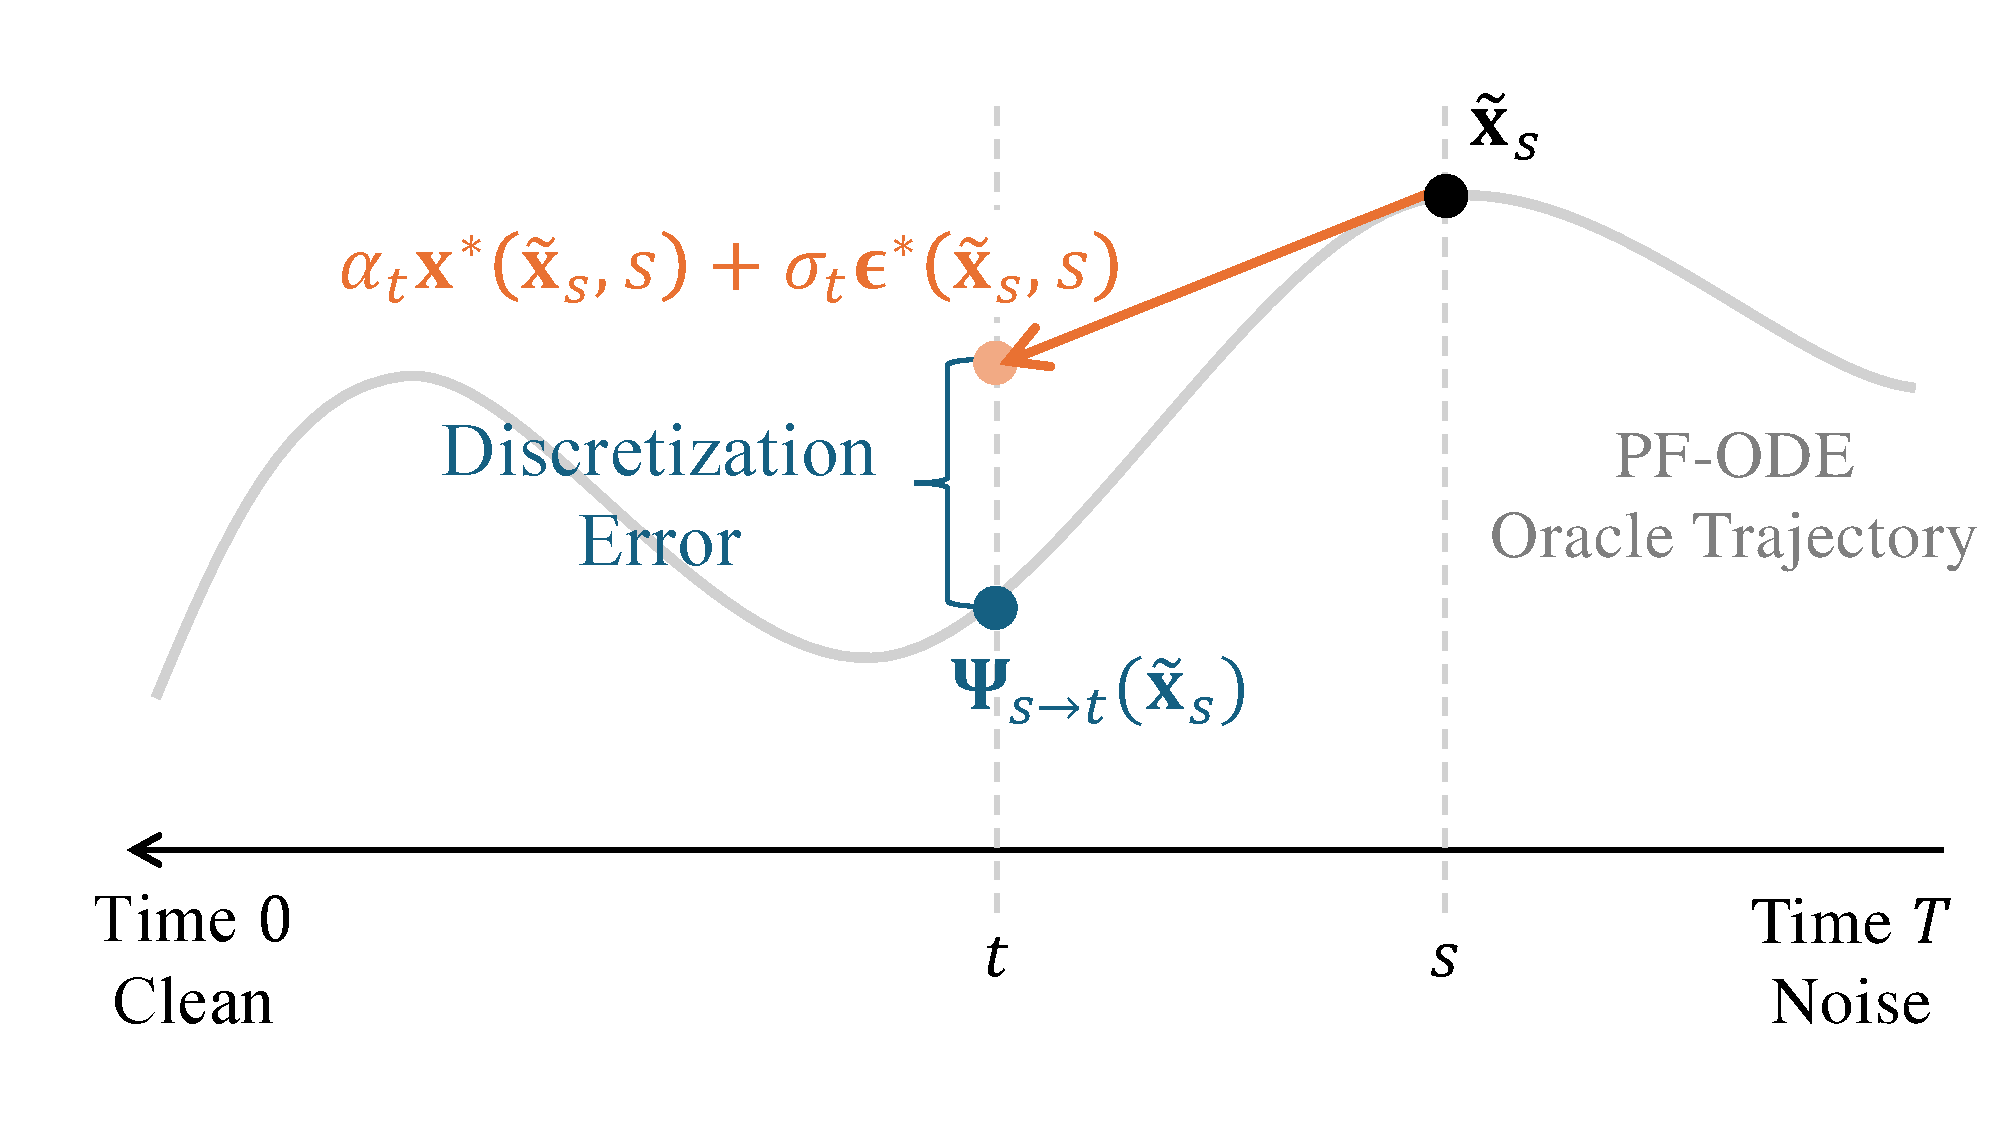
\includegraphics[width=\linewidth]{Images/PartB/Euler.pdf}
    \caption{\textbfs{将 DDIM 视为 PF-ODE 的 Euler 离散化的示意图。}  从时刻 $s$ 的状态 $\tilde\rvx_s$ 出发，真实 PF-ODE 轨迹（灰色曲线）确定性地演化到时刻 $t$ 的 $\bPsi_{s\to t}(\tilde\rvx_s)$。相比之下，DDIM 更新（橙色）直接将 $\tilde\rvx_s$ 映射到 $\alpha_t \rvx^*(\tilde\rvx_s,s) + \sigma_t \beps^*(\tilde\rvx_s,s)$。该 Euler 步与真实 PF-ODE 轨迹之间的差异引入了离散化误差，以蓝色显示。如果 $t$ 远离 $s$，差异可能变得很大，从而导致生成质量下降。
\figcredit{由作者绘制。}}
    \label{fig:euler}
\end{figure}


采用速度预测时，PF-ODE 中的线性项 $f(t)\rvx$ 被吸收到目标 $\rvv^*(\rvx(t), t)=\alpha_t'\rvx_0+\sigma_t'\beps$ 之中。由微积分基本定理，
积分 $\int_s^t \alpha_\tau'\diff\tau$ 与 $\int_s^t \sigma_\tau'\diff\tau$
简化为 $(\alpha_t-\alpha_s)$ 与 $(\sigma_t-\sigma_s)$，因此单个 Euler 步
就已经给出闭式的 DDIM 更新：
\[
\tilde\rvx_t = \alpha_t \tilde\rvx^*(\tilde\rvx_s,s) + \sigma_t \tilde\beps^*(\tilde\rvx_s,s).
\]

也就是说，采用 $\rvv$-预测时，PF-ODE 漂移中不存在需要单独分离的线性项，
因此朴素 Euler 更新自然地与 DDIM 表述一致。
相比之下，在 $\beps$-、$\rvx$-或 $\rvs$-预测参数化下，
PF-ODE 漂移可以分解为\emph{半线性}形式，由一个线性项和一个非线性修正构成，
这符合 \Cref{eq:general-semilinear-pfode} 给出的一般模板。于是，朴素的 Euler 步只能\emph{近似}线性项，而非精确计算它
（见 \Cref{eq:euler-step} 中的论证）。而 DDIM 对应于一种\emph{指数 Euler}（积分因子）步，
它解析地处理这一线性分量。
因此，$\rvv$-预测带来了最简单、最直接的 Euler 积分，
而其它参数化则需要指数 Euler 形式才能达到相同的 DDIM 行为。

上面的讨论也呼应了 \Cref{subsec:concept-why-v-affine} 中提出的论证，
并导出如下结论：
\msg{观察}{（指数）Euler 与 DDIM 更新}{
给定相同的调度器 $(\alpha_t,\sigma_t)$，
\begin{align*}
\text{$\rvv$-预测：} 
&\quad \text{Euler} = \text{DDIM}, \\[4pt]
\text{$\beps$-、$\rvx$-或 $\rvs$-预测：} 
&\quad \text{exp--Euler} = \text{DDIM} \neq \text{plain Euler},
\end{align*}
其中在 $\beps$-、$\rvx$-或 $\rvs$-预测情形下，朴素 Euler 步不等价于 DDIM，
因为线性项仅是被近似，可能导致稳定性降低。
}





\paragraph{不同参数化下 DDIM 的示例。}
我们用一个基于 \Cref{eq:ddim-update-all}、采用真实替换（$\beps^*$、$\rvx^*$、$\nabla_\rvx\log p_t$ 与 $\rvv^*$）的简单示例来说明。
假设前向核 $\alpha_t=1$ 且 $\sigma_t=t$~\citep{karras2022elucidating}。DDIM（exp--Euler）更新
\[
\tilde\rvx_{t} = \frac{\alpha_{t}}{\alpha_{s}}\tilde\rvx_{s}
- \alpha_{t} \left(\frac{\sigma_{s}}{\alpha_{s}} - \frac{\sigma_{t}}{\alpha_{t}}\right)
\beps^*(\tilde\rvx_{s}, s)
\]
简化为
\[
\tilde\rvx_t = \tilde\rvx_s - (s-t)\,\beps^*(\tilde\rvx_s,s).
\]
直观上，减去时间间隔 $(s-t)$ 与真实噪声估计
$\beps^*(\tilde\rvx_s,s)$ 的乘积，会将当前样本 $\tilde\rvx_s$ 推向更干净的估计。

使用 $\rvx$-预测的真实值 $\rvx^*$，它与噪声真实值的关系为
\[
\beps^*(\tilde\rvx_s,s) = \frac{\tilde\rvx_s - \rvx^*(\tilde\rvx_s, s)}{s},
\]
得到
\begin{align}\label{eq:ctm-formulation}
    \tilde\rvx_t
 = \tilde\rvx_s - \frac{s-t}{s}\,\bigl(\tilde\rvx_s - \rvx^*(\tilde\rvx_s, s)\bigr)
 = \frac{t}{s}\,\tilde\rvx_s + \Bigl(1-\frac{t}{s}\Bigr)\,\rvx^*(\tilde\rvx_s, s).
\end{align}
因此，$\tilde\rvx_t$ 是当前样本 $\tilde\rvx_s$ 与 $\rvx$-预测 $\rvx^*(\tilde\rvx_s, s)$（作为干净数据的真实估计）的凸组合。进一步地，我们可将其改写为
\[
\tilde\rvx_t-\rvx^* = \frac{t}{s}\,\bigl(\tilde\rvx_s-\rvx^*\bigr),\quad t<s,
\]
这表明去噪残差在每步按因子 $t/s\in(0,1)$ 收缩（因此当 $t<s$ 时不会出现超调）。

使用分数真实值，它与噪声真实值的关系为
\[
\beps^*(\tilde\rvx_s, s) = -\sigma_s \nabla_{\rvx}\log p_s(\tilde\rvx_s),
\]
DDIM（exp--Euler）更新变为
\[
\tilde\rvx_t = \tilde\rvx_s + (s-t)\,s\,\nabla_{\rvx}\log p_s(\tilde\rvx_s).
\]
这使 $\tilde\rvx_s$ 沿分数场上坡移动（朝更高似然区域），步长与时间间隔 $(s-t)$ 和噪声尺度 $s$ 成正比。

最后，使用速度真实值 $\rvv^*(\tilde\rvx_s,s) = \beps^*(\tilde\rvx_s,s)$，DDIM 更新可写为
\[
\tilde\rvx_t = \tilde\rvx_s + (t-s)\,\rvv^*(\tilde\rvx_s,s),
\]
于是割线斜率满足有限差分恒等式
\[
\frac{\tilde\rvx_t-\tilde\rvx_s}{t-s} = \rvv^*(\tilde\rvx_s,s).
\]
直观上，这意味着更新是沿局部 ODE 漂移方向的直线步。


\paragraph{DDIM 的挑战。}
作为一阶方法，DDIM 的全局离散化误差为
$\mathcal O(h)$，其中 $h:=\max_i |t_i-t_{i-1}|$。相应地，其
精度通常随步长增大而下降。这促使了高阶求解器的出现，
它们使用更丰富的局部近似把全局阶数提升到 $\mathcal O(h^k)$（$k\ge 2$）。
经过合适的时间步分配，这类方法可在更少的步数下达到目标质量。
然而，单凭更高阶并不能保证实际耗时更低，
因为每步可能需要多次模型求值。
在实践中，效率的相关度量是函数评估次数 $\mathrm{NFE}=mN$，
因此“更快”意味着以更小的 NFE 达到期望的质量，而不仅仅是更少的步数。

这个全局 $\mathcal O(h)$ 的论断虽然正确，但过于粗略，
无法解释为何某些 PF-ODE 轨迹即使在相对大的步长下也能保持良好的近似，
而另一些则不然。更具信息量的视角是询问：DDIM 在每一步冻结的是什么量，
以及该量沿精确轨迹变化有多大。

\paragraph{真正决定 DDIM 一阶误差的因素。}
一个重要的澄清是，参数化的选择\emph{并不}改变精确的真实 PF-ODE 轨迹。
在 \Cref{eq:predictions-equivalence} 的真实恒等式下，
$\rvv$-、$\beps$-、$\rvx$-与 $\rvs$-参数化只是同一 ODE 的不同表示。
所改变的只是漂移写出的形式，从而是一阶离散化把哪个量当作近似常数来处理。

\subparagraph{$\rvv$-预测情形（DDIM = Euler）。}
对 $\rvv$-预测，DDIM 恰好是对
\[
\frac{\diff \rvx(\tau)}{\diff \tau}=\rvv(\rvx(\tau),\tau).
\]
的朴素 Euler 步。
设 $h:=s-t>0$，其中 $s>t$。从时刻 $s$ 的精确状态 $\rvx_s$ 出发，
单步 DDIM/Euler 更新为
\[
\tilde{\rvx}_t^{\mathrm{Euler}}
=
\rvx_s-h\,\rvv(\rvx_s,s).
\]
带积分余项的 Taylor 定理给出
\[
\rvx(t)-\tilde{\rvx}_t^{\mathrm{Euler}}
=
\int_t^s (\tau-t)\,
\frac{\diff}{\diff \tau}\rvv(\rvx(\tau),\tau)\,\diff\tau,
\]
其中
\[
\frac{\diff}{\diff \tau}\rvv(\rvx(\tau),\tau)
=
\partial_\tau \rvv(\rvx(\tau),\tau)
+
\nabla_{\rvx}\rvv(\rvx(\tau),\tau)\,\rvv(\rvx(\tau),\tau).
\]
因此
\[
\|\rvx(t)-\tilde{\rvx}_t^{\mathrm{Euler}}\|
\le
\frac{h^2}{2}\,
\sup_{\tau\in[t,s]}
\Big\|
\partial_\tau \rvv(\rvx(\tau),\tau)
+
\nabla_{\rvx}\rvv(\rvx(\tau),\tau)\,\rvv(\rvx(\tau),\tau)
\Big\|.
\]
于是，对朴素 Euler 而言，相关的量是漂移沿精确轨迹求值的总时间导数
\[
\frac{\diff}{\diff \tau}\rvv(\rvx(\tau),\tau),
\]
等价地即轨迹的加速度，它度量了路径在该步内的弯曲程度。
特别地，若精确轨迹在 $[t,s]$ 上关于时间是仿射的，
则 Euler 在该步上是精确的。这是底层真实轨迹的特殊性质，
而非使用 $\rvv$-预测的一般结果。

\subparagraph{$\beps$-、$\rvx$-与 $\rvs$-预测情形（DDIM = Exp--Euler）。}
对 $\beps$-、$\rvx$-与 $\rvs$-预测，DDIM 是半线性 PF-ODE
\[
\frac{\diff \rvx(\tau)}{\diff \tau}
=
f(\tau)\rvx(\tau)+\rmN(\rvx(\tau),\tau).
\]
的指数 Euler 方法。
利用常数变易公式，
\[
\rvx(t)
=
\mathcal E(s\shortrightarrow t)\rvx_s
+
\int_s^t
\mathcal E(\tau\shortrightarrow t)\,
\rmN(\rvx(\tau),\tau)\,\diff\tau,
\qquad
\mathcal E(s\shortrightarrow t)
:=
\exp\!\Big(\int_s^t f(u)\,\diff u\Big),
\]
相应的指数 Euler 步为
\[
\tilde{\rvx}_t^{\mathrm{Exp}\text{-}\mathrm{Euler}}
=
\mathcal E(s\shortrightarrow t)\rvx_s
+
\left(\int_s^t \mathcal E(\tau\shortrightarrow t)\,\diff\tau\right)
\rmN(\rvx_s,s).
\]
将两个表达式相减得到精确恒等式
\[
\rvx(t)-\tilde{\rvx}_t^{\mathrm{Exp}\text{-}\mathrm{Euler}}
=
\int_s^t
\mathcal E(\tau\shortrightarrow t)\,
\Big(
\rmN(\rvx(\tau),\tau)-\rmN(\rvx_s,s)
\Big)\,\diff\tau.
\]
因此局部误差并非由 $\rvx(\tau)$ 字面意义上的笔直程度控制，
而是由非线性残差 $\rmN$ 沿精确轨迹的变化量控制。
若 $\mathcal E(\tau\shortrightarrow t)$ 在 $[t,s]$ 上有界，则
\[
\|\rvx(t)-\tilde{\rvx}_t^{\mathrm{Exp}\text{-}\mathrm{Euler}}\|
\le
\left(\sup_{\tau\in[t,s]}|\mathcal E(\tau\shortrightarrow t)|\right)
\frac{h^2}{2}\,
\sup_{\tau\in[t,s]}
\Big\|
\frac{\diff}{\diff \tau}\rmN(\rvx(\tau),\tau)
\Big\|,
\]
其中
\[
\frac{\diff}{\diff \tau}\rmN(\rvx(\tau),\tau)
=
\partial_\tau \rmN(\rvx(\tau),\tau)
+
\nabla_{\rvx}\rmN(\rvx(\tau),\tau)\,
\bigl(f(\tau)\rvx(\tau)+\rmN(\rvx(\tau),\tau)\bigr).
\]
特别地，每当 $\rmN(\rvx(\tau),\tau)$ 在该区间上保持常数时，
指数 Euler 在该步上是精确的。

要点并不在于某种参数化使真实 PF-ODE 轨迹变得“笔直”。
相反，少步精度由所选一阶格式所冻结的量沿精确轨迹变化的大小控制：
对朴素 Euler 是漂移 $\rvv$，对指数 Euler 是非线性残差 $\rmN$。
这也澄清了为何一般性的全局 $\mathcal O(h)$ 论断在实践中可能过于粗略。
两条轨迹可能具有截然不同的少步行为，
即使这种最坏情形的界看起来相似，
因为实际的单步误差由所实现的真实路径上的相应导数决定。

上文的讨论仅涉及数值求解器的离散化误差；在实践中，
总采样误差还包括模型失配以及所学网络中的近似误差。


\subsection{（可选）DDIM 的变分视角}\label{subsec:ddim}

事实上，DDIM 的动机来自通过变分视角重新审视 DDPM。
在 DDPM 中，反向过程与一个特定的马尔可夫前向转移核
$p(\rvx_t|\rvx_{t-\Delta t})$ 绑定，它强制要求小的步长
以便正确地近似多步后验。DDIM 摆脱了这一限制，
它观察到训练目标仅依赖于边缘扰动 $p_t(\rvx_t|\rvx_0)$，
而不依赖于具体的前向转移。这一洞察使我们能够直接从边缘构造反向动力学，
因此可以在保持边缘一致性的同时跳过中间步骤。
由于该转移被定义为对任意 $t<s$ 都将 $p_s(\rvx_s|\rvx_0)$ 映射到
$p_t(\rvx_t|\rvx_0)$，我们可以使用一个粗的时间网格，
其更新次数要少得多，从而减少模型求值次数，实现快速的少步采样。



\paragraph{重新审视 DDPM 的变分视角。}
在 DDPM 中，训练固定了一族边缘扰动核
$p_t(\rvx_t|\rvx_0)$ 并优化一个仅依赖于这些边缘的代理目标。
然而在采样时，反向条件分布是单步前向核下的贝叶斯后验：
\[
p(\rvx_{t-\Delta t}|\rvx_t,\rvx_0)
= \frac{p(\rvx_t|\rvx_{t-\Delta t})\,p_{t-\Delta t}(\rvx_{t-\Delta t}|\rvx_0)}
       {p_t(\rvx_t|\rvx_0)}.
\]
这把反向更新与\emph{特定}的前向转移 $p(\rvx_t|\rvx_{t-\Delta t})$ 绑定在一起。
如果人们试图通过增大 $\Delta t$ 同时复用相同的单步核来跳过步骤，
那么这就不再匹配真实的多步后验，通常会损害边缘分布。


\paragraph{DDIM 的原始动机。}
DDIM 观察到训练目标仅约束边缘 $p_t(\rvx_t|\rvx_0)$，而不约束
中间的反向转移。因此，人们可以\emph{指定}一族反向条件分布
${\color{orange}\pi(\rvx_t|\rvx_s,\rvx_0)}$（对任意 $t<s$），使其满足\emph{单步边缘一致性}\footnote{如果我们把 \Cref{eq:ddim-reverse-kernel-def} 中的“用户定义”反向转移核
$\pi$ 选为与“真实”条件分布完全相同：
${\color{orange}\pi(\rvx_t|\rvx_s,\rvx_0)} = p(\rvx_t|\rvx_s, \rvx_0)$，
则边缘一致性条件
   \[
\int {\color{orange}\pi(\rvx_t|\rvx_s,\rvx_0)}\,p_s(\rvx_s|\rvx_0)\diff \rvx_s
= p_t(\rvx_t|\rvx_0)
\] 
仅仅是条件联合分布的\emph{全概率法则}（也称\emph{塔性质}）的推论：
\[
p_t(\rvx_t|\rvx_0)
= \int p(\rvx_t,\rvx_s|\rvx_0)\diff \rvx_s
= \int p(\rvx_t|\rvx_s,\rvx_0)\,p_s(\rvx_s|\rvx_0)\diff \rvx_s.
\]
或者等价地，将贝叶斯后验显式地写成
\[
p(\rvx_t|\rvx_s,\rvx_0)
= \frac{p(\rvx_s|\rvx_t,\rvx_0)\,p_t(\rvx_t|\rvx_0)}
       {p_s(\rvx_s|\rvx_0)},
\]
然后两端乘以 $p_s(\rvx_s|\rvx_0)$ 并对 $\rvx_s$ 求边缘，我们恢复
\[
\int p(\rvx_t|\rvx_s,\rvx_0)\,p_s(\rvx_s|\rvx_0) \diff \rvx_s
= p_t(\rvx_t|\rvx_0),
\]
这恰好是相同的边缘一致性条件。

在马尔可夫前向情形下，进一步有
$p(\rvx_t|\rvx_s,\rvx_0)=p(\rvx_t|\rvx_s)$，
从而下式化简为：
\[
p_t(\rvx_t|\rvx_0)
= \int p(\rvx_t|\rvx_s)\,p_s(\rvx_s|\rvx_0)\diff \rvx_s.
\]
}：
\begin{mdframed}
    \begin{align}\label{eq:ddim-reverse-kernel-def}
\int {\color{orange}\pi(\rvx_t|\rvx_s,\rvx_0)}\,p_s(\rvx_s|\rvx_0) \diff \rvx_s
= p_t(\rvx_t|\rvx_0).
\end{align}
\end{mdframed}
这种构造消除了对前向单步核 $p(\rvx_t|\rvx_{t-\Delta t})$ 的任何依赖，
并为粗（跳过的）时间步提供了合法性。

\paragraph{离散时间 DDIM 的推导。}
考虑一般的前向扰动：
\begin{equation*}
    p_t(\rvx_t|\rvx_0) := \mathcal{N}\big(\rvx_t; \alpha_t \rvx_0, \sigma_t^2 \mathbf{I}\big),
\end{equation*}
其中 $\rvx_0 \sim p_{\mathrm{data}}$。


DDIM 不要求反向更新与绑定到
单步前向核的贝叶斯后验一致。只需\emph{选择}一个保持
边缘的反向条件分布即可。具体地，对任意 $t<s$ 我们假定高斯族
\begin{align}\label{eq:ddim-reverse-kernel-param}
{\color{orange}\pi(\rvx_t|\rvx_s,\rvx_0)}
= \mathcal{N} \big(\rvx_t;\, a_{t,s}\,\rvx_0 + b_{t,s}\,\rvx_s,\; c_{t,s}^2\,\mathbf{I}\big),
\end{align}
其系数 $(a_{t,s},b_{t,s},c_{t,s})$ 由边缘一致性
约束 \Cref{eq:ddim-reverse-kernel-def} 确定。由于所有涉及的核都是高斯的，
按 \Cref{eq:ddim-reverse-kernel-param} 从 $\rvx_s|\rvx_0=\alpha_s\rvx_0+\sigma_s\beps'$ 采样，然后再采样
$\rvx_t|\rvx_s,\rvx_0$，得到
\begin{align}\label{eq:ddim-derivation} 
\begin{aligned}
\rvx_t
&= a_{t,s}\,\rvx_0 + b_{t,s}\,\rvx_s + c_{t,s}\,\beps
\\&= a_{t,s}\,\rvx_0 + b_{t,s}\big(\alpha_s\rvx_0+\sigma_s\beps'\big) + c_{t,s}\,\beps \\
&= (a_{t,s} + b_{t,s}\alpha_s)\,\rvx_0
+ \sqrt{b_{t,s}^2\sigma_s^2 + c_{t,s}^2}\;\beps'',
\end{aligned}
\end{align}
其中 $\beps,\beps',\beps''\sim\mathcal{N}(\mathbf{0},\mathbf{I})$ 相互独立（高斯可加性）。
另一方面，
\[
\rvx_t\sim p_t(\rvx_t|\rvx_0)
= \mathcal{N} \big(\rvx_t; \alpha_t\rvx_0, \sigma_t^2\mathbf{I}\big).
\]
令此目标与 \Cref{eq:ddim-derivation} 的均值和方差相等，得到
\begin{align*}
\alpha_t = a_{t,s} + b_{t,s}\alpha_s,
\qquad
\sigma_t^2 = b_{t,s}^2\sigma_s^2 + c_{t,s}^2.
\end{align*}
这个方程组是欠定的，因此我们把 $c_{t,s}$ 视为带有自然约束
$0\le c_{t,s} \le \sigma_t$ 的自由参数，求解 $a_{t,s},b_{t,s}$：
\begin{align}\label{eq:ddim-coefficients}
b_{t,s} = \frac{\sqrt{\sigma_t^2 - c_{t,s}^2}}{\sigma_s},
\qquad
a_{t,s} = \alpha_t - \alpha_s\,b_{t,s}.
\end{align}
这里我们不失一般性地取 $b_{t,s}$ 的非负根。

将 \Cref{eq:ddim-coefficients} 代入 \Cref{eq:ddim-reverse-kernel-param} 得到
\begin{align}\label{eq:ddim-reverse-kernel-result}
{\color{orange}\pi(\rvx_t|\rvx_s,\rvx_0)}
= \mathcal{N} \Big(
\rvx_t;\;
\underbrace{\alpha_t\rvx_0
+ \frac{\sqrt{\sigma_t^2 - c_{t,s}^2}}{\sigma_s}\,(\rvx_s - \alpha_s\rvx_0)}_{\text{mean}},
\;\; c_{t,s}^2\mathbf{I}\Big).
\end{align}
等价地，\Cref{eq:ddim-reverse-kernel-result} 中的均值展开为
\[
\Big(\alpha_t - \alpha_s\frac{\sqrt{\sigma_t^2 - c_{t,s}^2}}{\sigma_s}\Big)\rvx_0
+ \Big(\frac{\sqrt{\sigma_t^2 - c_{t,s}^2}}{\sigma_s}\Big)\rvx_s.
\]

\lem{DDIM 系数}{ddim-coeff}{
设 ${\color{orange}\pi(\rvx_t|\rvx_s,\rvx_0)}$ 由 \Cref{eq:ddim-reverse-kernel-param} 给出。
若边缘一致性条件 \Cref{eq:ddim-reverse-kernel-def} 成立，则系数
恰好是 \Cref{eq:ddim-coefficients} 中的那些，其中 $0\le c_{t,s}\le \sigma_t$。
}

\rmkb{
\begin{enumerate}[leftmargin=*]
    \item 在 DDIM 中，我们\emph{选择}反向核 ${\color{orange}\pi(\rvx_t|\rvx_s,\rvx_0)}$ 满足
边缘一致性约束，而一般地
\[
{\color{orange}\pi(\rvx_t|\rvx_s,\rvx_0)}\neq p (\rvx_t|\rvx_s,\rvx_0),
\]
其中 $p (\rvx_t|\rvx_s,\rvx_0)$ 是与特定前向
单步核相关联的贝叶斯后验。由贝叶斯法则，
\[
p(\rvx_t|\rvx_s,\rvx_0)\;\propto\; p(\rvx_s|\rvx_t)\,p_t(\rvx_t|\rvx_0),
\]
此后验\emph{并不}是规定 $\pi$ 或训练所必需的。
    \item 仅在选择方差参数以匹配 DDPM 后验
方差的特殊情形下（即 \Cref{eq:eta-ddim} 中 $\eta=1$ 的设定），才有 ${\color{orange}\pi(\rvx_t|\rvx_s,\rvx_0)}=
p (\rvx_t|\rvx_s,\rvx_0)$；否则 ${\color{orange}\pi(\rvx_t|\rvx_s,\rvx_0)} \neq
p (\rvx_t|\rvx_s,\rvx_0)$。
    \item 不施加马尔可夫约束时，一般地 $p(\rvx_s|\rvx_t,\rvx_0)\neq p(\rvx_s|\rvx_t)$。
等式 $p(\rvx_s|\rvx_t,\rvx_0)=p(\rvx_s|\rvx_t)$ 绑定于一个特定的马尔可夫前向模型，
而 DDIM 在其反向构造中并不假设该模型。
\end{enumerate}
}


前向边缘 $\{p_t(\rvx_t|\rvx_0)\}_t$ 并不唯一地确定反向条件
转移。存在无穷多个满足
\Cref{eq:ddim-reverse-kernel-def} 的核
${\color{orange}\pi(\rvx_t|\rvx_s,\rvx_0)}$，其中任何一个都可以自由地规定。
参数 $c_{t,s}$ 为这一族建立索引，并控制
每次反向步 $s \to t$ 注入的噪声量。下面，我们介绍这一族 DDIM 求解器。





\paragraph{DDIM 采样器（步 $s\to t$）。}
DDIM 采样器由所选反向核 \Cref{eq:ddim-reverse-kernel-result} 中的 ${\color{orange}\pi(\rvx_t|\rvx_s,\rvx_0)}$，
通过用预训练模型的预测器替换 $\rvx_0$ 而得到。
使用 $\beps$-预测网络 $\beps_{\bm{\phi}^\times}$（即插即用，无需重训），令
\[
\rvx_{\bm{\phi}^\times}(\rvx_s,s)
:= \frac{\rvx_s - \sigma_s\,\beps_{\bm{\phi}^\times}(\rvx_s,s)}{\alpha_s},
\quad
p_{\bm{\phi}^\times}(\rvx_t|\rvx_s)
:= {\color{orange}\pi\big(\rvx_t\,\big|\,\rvx_s,\rvx_{\bm{\phi}^\times}(\rvx_s,s)\big)}.
\]
将 $\rvx_{\bm{\phi}^\times}$ 代入 \Cref{eq:ddim-reverse-kernel-result} 得到更新
\begin{mdframed}
\[
\rvx_t
= \frac{\alpha_t}{\alpha_s}\,\rvx_s
+\Big(\sqrt{\sigma_t^2 - c_{t,s}^2}-\frac{\alpha_t}{\alpha_s}\sigma_s\Big)\,
\beps_{\bm{\phi}^\times}(\rvx_s,s)
+ c_{t,s}\,\beps_t,
\quad \beps_t\sim\mathcal{N}(\mathbf{0},\mathbf{I}),
\]
\end{mdframed}
其中 $c_{t,s}\in[0,\sigma_t]$ 控制随机性。

为记号方便，定义前向因子
\[
\alpha_{t|s}:=\tfrac{\alpha_t}{\alpha_s},
\qquad
\sigma_{t|s}^2:=\sigma_t^2-\alpha_{t|s}^2\,\sigma_s^2,
\]
使得 $p(\rvx_t|\rvx_s)=\mathcal{N}(\alpha_{t|s}\rvx_s,\sigma_{t|s}^2\mathbf{I})$。于是采样器可写为
\[
\rvx_t
= \alpha_{t|s}\,\rvx_s
+\big(\sqrt{\sigma_t^2 - c_{t,s}^2}-\alpha_{t|s}\sigma_s\big)\,
\beps_{\bm{\phi}^\times}(\rvx_s,s)
+ c_{t,s}\,\beps_t.
\]

通过改变 $c_{t,s}$，可得到一族共享同一预训练扩散模型且无需重训的采样器：
\begin{itemize}
\item \textbfs{DDPM 步（后验方差）：}
$
c_{t,s}=\frac{\sigma_s}{\sigma_t}\,\sigma_{t|s}
$
使 ${\color{orange}\pi(\rvx_t|\rvx_s,\rvx_0)}$ 等于由单步前向核诱导的贝叶斯后验
$p(\rvx_t|\rvx_s,\rvx_0)$。
用其预测器替换 $\rvx_0$ 得到标准 DDPM 反向更新
$p_{\bm{\phi}^\times}(\rvx_t|\rvx_s)$，即在 $\alpha_t^2+\sigma_t^2=1$ 下的马尔可夫 DDPM 步（\Cref{eq:ddpm-sampling}）。

\item \textbfs{确定性 DDIM（$\eta=0$）：}
$
c_{t,s}=0
$
给出
\[
\rvx_t
= \alpha_{t|s}\rvx_s + \big(\sigma_t-\alpha_{t|s}\sigma_s\big)\beps_{\bm{\phi}^\times}(\rvx_s,s),
\]
与 ODE 视角下的 DDIM 跳跃一致。

\item \textbfs{插值：} 定义
\begin{align}\label{eq:eta-ddim}
    c_{t,s}=\eta\,\frac{\sigma_s}{\sigma_t}\,\sigma_{t|s}, \quad \eta\in[0,1],
\end{align}
使得 $\eta$ 在随机 DDPM 更新（$\eta=1$）与确定性 DDIM 更新（$\eta=0$）之间平滑插值。
\end{itemize}





\subsection{作为条件流匹配的 DDIM}\label{subsec:ddim-cfm}
本小节将看到，确定性 DDIM 可以被理解为寻找一个条件流映射，它把 $p_s(\cdot|\rvx_0)$ 前推到 $p_t(\cdot|\rvx_0)$。
此条件流的切线与条件流匹配（CFM）中使用的条件速度一致。
对该条件速度取边缘便得到 PF--ODE 漂移，其朴素 Euler 离散化恢复了 $\rvv$-预测下的边缘 DDIM 更新。

我们重新审视 DDIM 单步条件边缘一致性恒等式（\Cref{eq:ddim-reverse-kernel-def}）
\[
\int {\color{orange}\pi(\rvx_t|\rvx_s,\rvx_0)} p_s(\rvx_s|\rvx_0) \diff \rvx_s
= p_t(\rvx_t|\rvx_0), \quad t<s,
\]
即若 $\rvx_s\sim p_s(\cdot|\rvx_0)$，则用所选反向核前推 $\rvx_s$ 可复现 $p_t(\cdot|\rvx_0)$。
当反向核为确定性时，它等价于寻找一个条件映射
$\bPsi_{s\to t}(\cdot|\rvx_0)$，把 $p_s(\cdot|\rvx_0)$ 前推到 $p_t(\cdot|\rvx_0)$：
\[
{\color{orange}\pi(\rvx_t|\rvx_s,\rvx_0)}
=\delta \big(\rvx_t-\bPsi_{s\to t}(\rvx_s|\rvx_0)\big),
\qquad
\bigl(\bPsi_{s\to t}(\cdot|\rvx_0)\bigr)_{\#}p_s(\cdot|\rvx_0)=p_t(\cdot|\rvx_0).
\]


在线性--高斯路径 $\rvx_\tau=\alpha_\tau\rvx_0+\sigma_\tau\beps$ 下，
类似于 \Cref{eq:ddim-reverse-kernel-param,eq:ddim-derivation} 的论证
给出\textit{条件映射}
\[
\bPsi_{s\to t}(\rvx_s|\rvx_0)
=\frac{\sigma_t}{\sigma_s}\,\rvx_s
+\Bigl(\alpha_t-\alpha_s\frac{\sigma_t}{\sigma_s}\Bigr)\rvx_0,
\]
其瞬时的\textit{条件速度}为
\[
\rvv_t^{*}(\rvx|\rvx_0)
=\partial_h \big|_{h=0}\bPsi_{t\to t+h}(\rvx|\rvx_0)
=\frac{\sigma_t'}{\sigma_t}\,\rvx
+\Bigl(\alpha_t'-\alpha_t\frac{\sigma_t'}{\sigma_t}\Bigr)\rvx_0.
\]
我们将 $\bPsi_{s\to t}(\cdot|\rvx_0)$ 称为 DDIM 条件映射。

有了 $p_t(\rvx|\rvx_0)$，条件流匹配把时间依赖场拟合到此目标速度，
\[
\mathcal L_{\mathrm{CFM}}(\bphi)
=\E_{t,\rvx_0,\rvx_t\sim p_t(\cdot|\rvx_0)}
\big\|\rvv_\bphi(\rvx_t,t)-\rvv_t^{*}(\rvx_t|\rvx_0)\big\|^2,
\]
因此 CFM 的回归目标等于 DDIM 条件映射的条件速度。

\msg{观察}{条件层面}{
沿条件高斯路径，DDIM 条件映射与 CFM 目标生成相同的条件流 $\bPsi_{s\to t}(\cdot|\rvx_0)$。
}

在给定 $\rvx_t=\rvx$ 下对 $\rvx_0$ 的后验求条件速度的平均，得到边缘 PF--ODE 漂移，
\[
\rvv^*(\rvx,t)=\E \left[\rvv_t^*(\rvx| \rvx_0)|\rvx_t=\rvx\right],
\]
它在线性--高斯调度下取可分离的预测器形式
\[
\rvv^*(\rvx,t)=\alpha_t'\,\rvx^*(\rvx,t)+\sigma_t'\,\beps^*(\rvx,t),
\quad
\rvx=\alpha_t\,\rvx^*(\rvx,t)+\sigma_t\,\beps^*(\rvx,t).
\]
我们已经看到，对此取过边缘的 $\rvv$-预测的 PF-ODE，其朴素 Euler 步恰好是 DDIM 更新（\Cref{eq:ddim-update-all} 中最后的恒等式）。

简言之，DDIM 是（i）一个确定性条件传输，其切线等于 CFM 目标；（ii）对该切线取边缘后，是 PF--ODE 的一个 Euler 步，其步恰好与 DDIM 更新一致。


\newpage


% \paragraph{(Optional, move to appendix) Gauge freedom and rotations}
% More generally, one may replace the shared-noise coupling with any orthogonal transformation
% $\rmR_{s\to t}\in\mathrm{O}(D)$, yielding
% \[
% \rmT^{\rvx_0}_{s\to t}(\rvx_s)
% =\frac{\sigma_t}{\sigma_s}\,\rmR_{s\to t}\,\rvx_s
% +\Big(\alpha_t-\alpha_s\frac{\sigma_t}{\sigma_s}\,\rmR_{s\to t}\Big)\rvx_0,
% \qquad
% \beps_t=\rmR_{s\to t}\beps_s.
% \]
% Each such choice preserves the marginal consistency condition, introducing a \emph{gauge freedom} in the noise rotation.
% For the maps to compose consistently across time, the rotations must satisfy the cocycle (semigroup) rule
% \[
% \rmR_{s\to t}=\rmR_{u\to t}\,\rmR_{s\to u},\qquad
% \rmR_{t\to t}=\rmI.
% \]
% DDIM corresponds to the simplest gauge, $\rmR_{s\to t}=\rmI$, where all noise directions are aligned (shared across time).
% Since this specific gauge already yields the standard DDIM flow and serves as the target for CFM,
% the broader rotation family is optional and mainly of theoretical interest.

%%%%%%%%%%%%%%%%%%%%%%%%%%%%
% In this subsection, we further focus on the discussion on the (variational perspective) DDIM marginal-consistency identity (\Cref{eq:ddim-reverse-kernel-def})
% \begin{align*}
% \int {\color{orange}\pi(\rvx_t|\rvx_s,\rvx_0)}p_s(\rvx_s|\rvx_0)\diff \rvx_s
% = p_t(\rvx_t|\rvx_0), \quad t<s.
% \end{align*}
% It states that, if $\rvx_s\sim p_s(\cdot|\rvx_0)$, then pushing $\rvx_s$ forward by the
% user-specified kernel ${\color{orange}\pi(\cdot|\rvx_s,\rvx_0)}$ produces the correct later marginal
% $p_t(\cdot|\rvx_0)$.


% \paragraph{Deterministic Kernels $\Rightarrow$ Pushforward Maps.}
% When the reverse kernel ${\color{orange}\pi(\rvx_t|\rvx_s,\rvx_0)}$ is chosen to be \emph{deterministic}, it can be written as a Dirac measure
% concentrated at the output of a conditional map $\rmT^{\rvx_0}_{s\to t}$:
% \[
% {\color{orange}\pi(\rvx_t|\rvx_s,\rvx_0)}
% = \delta \big(\rvx_t-\rmT^{\rvx_0}_{s\to t}(\rvx_s)\big),
% \]
% Here, $\rmT^{\rvx_0}_{s\to t}(\cdot):\R^D \to \R^D$ is a function that evolves the state from time $s$ to time $t$ given a endpoint $\rvx_0$.

% In this case, one-step marginal consistency becomes searching a conditional (on $\rvx_0$) deterministic map $\rmT^{\rvx_0}_{s\to t}$ that satisfies the  pushforward relation
% \[
% (\rmT^{\rvx_0}_{s\to t})_{\#}\,p_s(\cdot|\rvx_0)=p_t(\cdot|\rvx_0).
% \]

% \paragraph{Gaussian Forward and the General Form of a Marginal-Correct Map.}
% Assume the standard linear–Gaussian forward conditionals
% \[
% p_\tau(\rvx_\tau|\rvx_0)=\mathcal N \big(\rvx_\tau;\alpha_\tau \rvx_0,\;\sigma_\tau^2 \rmI\big),\qquad \sigma_\tau>0.
% \]
% If a deterministic map pushes $p_s(\cdot|\rvx_0)$ to $p_t(\cdot|\rvx_0)$ for \emph{all} $\rvx_0$, then (classically) it must be
% \emph{affine}:
% \[
% \rmT^{\rvx_0}_{s\to t}(\rvx_s)=\rmA_{s\to t}\rvx_0 + \rmB_{s\to t}\rvx_s,
% \]
% and matching the Gaussian mean and covariance forces
% \[
% \rmA_{s\to t}=\alpha_t\rmI-\alpha_s\frac{\sigma_t}{\sigma_s}\rmR_{s\to t},\quad 
% \rmB_{s\to t}=\frac{\sigma_t}{\sigma_s}\rmR_{s\to t}
% \]
% where $\rmR_{s\to t}$ is any $D\times D$ orthogonal matrix.
% Hence the more general deterministic, marginal-correct update (oracle case) is
% \[
% \rmT^{\rvx_0}_{s\to t}(\rvx_s)
% =\frac{\sigma_t}{\sigma_s}\rmR_{s\to t}\,\rvx_s
% +\Big(\alpha_t-\alpha_s\frac{\sigma_t}{\sigma_s}\rmR_{s\to t}\Big)\rvx_0.
% \]
% The orthogonal factor $\rmR_{s\to t}$ is a genuine \emph{gauge freedom}: it does not change the one-step marginals.


% \paragraph{Route to Standard DDIM.}
% For any fixed $\rvx_0$, if the family $\{\rmT^{\rvx_0}_{s\to t}(\cdot)\}_{s,t}$ is continuous in $t$,
% locally Lipschitz in $\rvx$, and satisfies $\rmT^{\rvx_0}_{t\to t}=\mathrm{Id}$, then it constitutes the
% \emph{conditional flow map} (evolution family) of an ODE. We write this conditional flow map as $ \bPsi_{s\to t}(\cdot|\rvx_0)$ to replace $\rmT^{\rvx_0}_{s\to t}(\cdot)$. Its conditional velocity is derived (?) defined (?) in the following sense: by taking time differentiation:
% \[
% \rvv_t(\rvx|\rvx_0):= \lim_{h\to 0}\frac{\big(\bPsi_{t\to t+h}(\rvx|\rvx_0)-\rvx\big)}{h}, \quad\text{for any }\, t
% \]
% whenever the limit exists. Standard existence and uniqueness results for ODEs then ensure that this conditional
% vector field generates the given  conditional flow (i.e., the  continuity equation is fulfilled). 

% Since $ \bPsi_{s\to t}(\cdot|\rvx_0)$ is an ODE flow map, the following holds automatically by uniqueness, which is known as \emph{semigroup property} for flow maps:
% \[
% \bPsi_{s\to t}(\cdot|\rvx_0)=\bPsi_{u\to t}(\cdot|\rvx_0) \circ \bPsi_{s\to u}(\cdot|\rvx_0),
% \quad
% \bPsi_{t\to t}(\cdot|\rvx_0)=\mathrm{Id}.
% \]
% This implies the rotation matrix (gauge freedom) $\rmR_{s\to t}$ needs to satisfies: 
% \[
% \rmR_{s\to t} = \rmR_{u\to t} \circ \rmR_{s\to u},
% \]
% while there are infinitely many choices for this rotation matrix.

% In the standard DDIM, condition on $\rvx_0$ and pick the path $\rvx_t=\alpha_t \rvx_0+\sigma_t\beps$ with \emph{shared} $\beps$. It fixes the gauge freedom by the \emph{shared-noise}  $\beps\sim \mathcal{N}(\bm{0}, \rmI)$ choice:
% \[
% \beps_t=\beps_s=\beps,\quad \text{for any }\, s>t.
% \]
% This is equivalent to enforcing   $\rmR_{s\to t}=\rmI$ for all $s>t$. 

% With this shared noise, it leads to the standard DDIM deterministic update:
% \[
% \bPsi_{s\to t}(\rvx_s| \rvx_0)
% =\frac{\sigma_t}{\sigma_s}\,\rvx_s+\Big(\alpha_t-\alpha_s\frac{\sigma_t}{\sigma_s}\Big)\rvx_0.
% \]


% \paragraph{How this Connects to Flow Matching.}

% Its time derivative gives a \emph{conditional velocity}
% \[
% \rvv_t(\rvx| \rvx_0)=\alpha_t' \rvx_0+\frac{\sigma_t'}{\sigma_t}\big(\rvx-\alpha_t\rvx_0\big).
% \]
% \emph{Conditional Flow Matching} trains a model to match this drift; integrating it recovers the DDIM map above.
% Unconditioning (averaging over $\rvx_0$ given $\rvx_t$) yields the familiar probability-flow ODE drift used in score-based samplers.

% \paragraph{Practical note.}
% At sampling time, $\rvx_0$ is unknown and replaced by a denoiser  $\rvx_{\bphi^\times}(\rvx_s,s)$, so both one-step marginal matching and semigroup hold only \emph{approximately}. Enforcing composition (CK/semigroup) during design or training can improve robustness to step size, but the core DDIM update follows already from one-step marginals plus the shared-noise gauge.


%%%%%%%%%%%%%%%%%%%%%%%%%%%%%
% \paragraph{(Optional) Chapman--Kolmogorov Identity vs.\ Semigroup Property.}
% Important: the pushforward relationship does not force different time pairs to be compatible. You can satisfy all pairs $(s,t)$ and still have
% $\rmT^{\rvx_0}_{t\to u} \circ \rmT^{\rvx_0}_{s\to t}\neq \rmT^{\rvx_0}_{s\to u}$.


% The Chapman--Kolmogorov (CK) identity composes kernels across an intermediate time:
% \[
% \pi_{s\to u}(\rvx_u|\rvx_s,\rvx_0)
% =\int \pi_{t\to u}(\rvx_u|\rvx_t,\rvx_0)\,\pi_{s\to t}(\rvx_t|\rvx_s,\rvx_0)\diff\rvx_t\quad(s>t>u).
% \]
% In the deterministic case this reduces to the \emph{semigroup property} for maps
% \[
% \rmT^{\rvx_0}_{s\to u}=\rmT^{\rvx_0}_{t\to u}\circ \rmT^{\rvx_0}_{s\to t},
% \qquad
% \rmT^{\rvx_0}_{t\to t}=\mathrm{Id}.
% \]
% CK/semigroup is strictly \emph{stronger} than one-step marginal consistency.



%%%%%%%%%%%%%%%%%%%%%%%%%%

% ---------
% DDIM relaxes the Markovian assumption in the reverse (inference) process to enable fast sampling; defining the reverse transitions as Markovian is unnecessary. Instead, infinitely many choices exist for
% $p(\rvx_{t-\Delta t}|\rvx_t, \rvx_0)$ (i.e., there are infinitely many valid reverse transition distributions that map from $\mathbf{x}_t$ to $\mathbf{x}_{t-\Delta t}$ given $\mathbf{x}_0$), as long as the marginal consistency condition is satisfied:
% \begin{align}\label{eq:marginal_ddim}
%     \int p(\rvx_{t-\Delta t}|\rvx_t, \rvx_0)   p_t(\rvx_t|\rvx_0)   \diff\rvx_t = p_{t-\Delta t}(\rvx_{t-\Delta t}|\rvx_0).
% \end{align}

% We assume that $p(\rvx_{t-\Delta t}|\rvx_t, \rvx_0)$ is Gaussian, which is natural given the Gaussian forward kernels, and take it in the form:
% \begin{align}\label{eq:ddim-reverse-kernel-def}
%     p(\rvx_{t-\Delta t}|\rvx_t, \rvx_0) := \mathcal{N}\big(\rvx_{t-\Delta t}; a_t \rvx_0 + b_t \rvx_t, c_t^2 \mathbf{I}\big),
% \end{align}
% where coefficients $a_t, b_t, c_t$ are to be determined by \Cref{eq:marginal_ddim}. Since all involved kernels are Gaussian, the marginal consistency condition expands to
% \begin{align}\label{eq:ddim-derivation}
% \begin{aligned}
%     \rvx_{t-\Delta t} 
%     &= a_t \rvx_0 + b_t \rvx_t + c_t \bm{\epsilon} \\
%     &= a_t \rvx_0 + b_t (\alpha_t \rvx_0 + \sigma_t \bm{\epsilon}') + c_t \bm{\epsilon} \\
%     &= (a_t + b_t \alpha_t) \rvx_0 + \sqrt{(b_t \sigma_t)^2 + c_t^2} \bm{\epsilon}'',
% \end{aligned}
% \end{align}
% where $\bm{\epsilon}, \bm{\epsilon}', \bm{\epsilon}'' \sim \mathcal{N}(\bm{0}, \mathbf{I})$ are independent and we used the Gaussian sum property.

% On the other hand, from the forward process,
% \[
% \rvx_{t-\Delta t} \sim p_{t-\Delta t}(\rvx_{t-\Delta t}|\rvx_0) = \mathcal{N}\big(\rvx_{t-\Delta t}; \alpha_{t-\Delta t} \rvx_0, \sigma_{t-\Delta t}^2 \mathbf{I}\big),
% \]
% so equating means and variances in \Cref{eq:ddim-derivation} yields
% \begin{align}
% \begin{cases}
%     \alpha_{t-\Delta t} = a_t + b_t \alpha_t, \\
%     \sigma_{t-\Delta t} = \sqrt{(b_t \sigma_t)^2 + c_t^2}.
% \end{cases}
% \end{align}
% Since this system is underdetermined (i.e., has infinitely many solutions), we can treat $c_t$ as a free parameter and solve for $a_t$ and $b_t$, summarizing the result in the following lemma.
% \lem{DDIM Coefficients}{ddim-coeff}{
% Define the reverse conditional kernel as in \Cref{eq:ddim-reverse-kernel-def} with coefficients $a_t, b_t, c_t$. If it satisfies the marginal condition \Cref{eq:marginal_ddim}, then
% \begin{align*}
%     a_t &= \alpha_{t-\Delta t} - \alpha_t \frac{\sqrt{\sigma_{t-\Delta t}^2 - c_t^2}}{\sigma_t}, \quad
%     b_t = \frac{\sqrt{\sigma_{t-\Delta t}^2 - c_t^2}}{\sigma_t}.
% \end{align*}
% }
% Hence,
% \begin{align}\label{eq:ddim-reverse-kernel-result}
% \begin{aligned}
%     p(\rvx_{t-\Delta t}|\rvx_t, \rvx_0) = \mathcal{N}\Bigg(&
%         \rvx_{t-\Delta t}; 
%         \left(\alpha_{t-\Delta t} - \alpha_t \frac{\sqrt{\sigma_{t-\Delta t}^2 - c_t^2}}{\sigma_t}\right) \rvx_0 \\
%         &\quad+ \left(\frac{\sqrt{\sigma_{t-\Delta t}^2 - c_t^2}}{\sigma_t}\right) \rvx_t,
%         c_t^2 \mathbf{I}
%     \Bigg).
% \end{aligned}
% \end{align}
% \rmkb{
% Note that in the DDIM setup, in general,
% \[
% p(\rvx_t|\rvx_{t-\Delta t}, \rvx_0) \neq p(\rvx_t|\rvx_{t-\Delta t}),
% \]
% since the Markov assumption is not imposed. An analogous identity from Bayes' rule states that
% \[
% p(\rvx_{t-\Delta t}|\rvx_t, \rvx_0) = p(\rvx_t|\rvx_{t-\Delta t}, \rvx_0) \frac{p_{t-\Delta t}(\rvx_{t-\Delta t}|\rvx_0)}{p_t(\rvx_t|\rvx_0)}.
% \]
% Although we can compute $p(\rvx_t|\rvx_{t-\Delta t}, \rvx_0)$ using this identity, it is generally not used for training or sampling.\dk{Isn't it used to derive Eq. (2.2.3)? Other than thsi Bayes rule, how could we derive the loss function?}
% }
% Until now, we emphasize the key insight behind the DDIM approach from a variational perspective:
% \msg{Insight}{}{
% The forward marginal distributions $\{p_t(\rvx_t|\rvx_0)\}_t$ alone do not uniquely determine the reverse conditional transitions; in fact, there are infinitely many $p(\rvx_{t-\Delta t}|\rvx_t, \rvx_0)$ satisfying the marginal consistency (e.g., parameterized by $c_t$).
% }



% \paragraph{Discrete-Time DDIM Sampler.}  
% The key difference between DDIM and the formulation in DDPM (\Cref{sec:variational-perspective}) lies in modeling the conditional distribution $p(\rvx_{t-\Delta t}|\rvx_t, \rvx_0)$. Thus, DDIM enables a plug-and-play approach\footnote{See Theorem 1 in \citep{song2020denoising}.} to leverage any pre-trained diffusion model without retraining. 

% Here, we adapt the $\beps$-prediction model $\bm{\epsilon}_{\bm{\phi}^\times}$ as in the original DDPM, which can be easily converted to clean or other prediction forms via \Cref{eq:predictions-equivalence}. This defines the parameterized density
% \begin{align*}
%     p_{\bm{\phi}^\times}(\rvx_{t-\Delta t} |\rvx_t) := p\big(\rvx_{t-\Delta t} |\rvx_t, \rvx_{\bm{\phi}^\times}(\rvx_t, t)\big),
% \end{align*}
% where the ``clean data'' $\rvx_0$ in \Cref{eq:ddim-reverse-kernel-result} is replaced by the clean estimate $\rvx_{\bm{\phi}^\times}$, but expressed in terms of the $\beps$-prediction model as
% \[
% \rvx_{\bm{\phi}^\times}(\rvx_t, t) = \frac{\rvx_t - \sigma_t \bm{\epsilon}_{\bm{\phi}^\times}(\rvx_t, t)}{\alpha_t}.
% \]
% Sampling with $p_{\bm{\phi}^\times}(\rvx_{t-\Delta t}|\rvx_t)$ yields the DDIM sampler in the $\beps$-prediction form:
% \begin{mdframed}
% \begin{align*}
% \rvx_{t-\Delta t}
% = \frac{\alpha_{t-\Delta t}}{\alpha_t} \rvx_t
% + \sigma_t \left(\frac{\sqrt{\sigma_{t-\Delta t}^2 - c_t^2}}{\sigma_t}
% - \frac{\alpha_{t-\Delta t}}{\alpha_t}\right) 
% \bm{\epsilon}_{\bm{\phi}^\times}(\rvx_t,t)
% + c_t \bm{\epsilon}_t,
% \end{align*}
% \end{mdframed}
% where $c_t\in[0,\sigma_{t-\Delta t}]$ controls stochasticity and $\bm{\epsilon}_t\sim\mathcal N(\mathbf 0,\mathbf I)$.
% For notational simplicity, define the forward Markov factors
% \[
% \alpha_{t|s}:=\frac{\alpha_t}{\alpha_s},\quad
% \sigma_{t|s}^2:=\sigma_t^2-\alpha_{t|s}^2 \sigma_s^2,
% \]
% so that $p(\rvx_t|\rvx_s)=\mathcal N(\alpha_{t|s}\rvx_s,\sigma_{t|s}^2\mathbf I)$. Different choices of $c_t$ give a family of samplers using the same pre-trained diffusion model (no retraining):
% \begin{itemize}
%   \item \textbfs{DDPM (Variational Diffusion Model) Step:} If ($s=t-\Delta t$)
%   \[
%   c_t  =  \frac{\sigma_s}{\sigma_t}\sigma_{t|s},
%   \]
%   the update reduces to \Cref{eq:general-ddpm-sampling-discrete}\footnote{Here, the reverse process is Markovian.}. In particular, under $\alpha_t^2+\sigma_t^2=1$ it recovers \Cref{eq:ddpm-sampling}.
%   \item \textbfs{Deterministic DDIM:} If $c_t=0$,
%   \[
%   \rvx_{t-\Delta t}
%   = \frac{\alpha_{t-\Delta t}}{\alpha_t}\rvx_t
%   + \sigma_t \left(\frac{\sigma_{t-\Delta t}}{\sigma_t}
%   - \frac{\alpha_{t-\Delta t}}{\alpha_t}\right) 
%   \bm{\epsilon}_{\bm{\phi}^\times}(\rvx_t,t),
%   \]
%   which matches \Cref{eq:ddim-euler} from the ODE-solver view. We refer to \Cref{eq:ddim-update-all} for a summary of the deterministic DDIM update under
% different parameterizations of the diffusion model.
%   \item \textbfs{Interpolation:} For $\eta\in[0,1]$,
%   \[
%   c_t  =  \eta \frac{\sigma_s}{\sigma_t}\sigma_{t|s}
%   \]
%   interpolates between DDPM ($\eta=1$) and deterministic DDIM ($\eta=0$).
% \end{itemize}
% Thus the (stochastic) DDIM solver bridges \Cref{eq:general-ddpm-sampling-discrete} and deterministic DDIM by tuning $c_t$.

% By employing DDIM updates, one can use larger timesteps during sampling, which makes it possible to skip certain steps since the Markov assumption is no longer required. This reduces the number of sampling steps drastically, from the typical 1,000 in DDPM and Score SDE (with numerical solvers) to around 50 to 100, a significant practical advantage.

% \rmkb{Many works formulate the DDIM solver based on DDPM’s perturbation kernel with the constraint $\alpha_t^2 + \sigma_t^2 = 1$. However, as shown here, DDIM is more general and applies to any Gaussian perturbation kernel without this restriction.}


\clearpage
\newpage



\section{\texorpdfstring{DEIS}{DEIS}}\label{sec:exponential}
在指数积分器公式（\Cref{eq:variation_of_constants}）中，
\[
\int_{s}^{t}
\frac{g^2(\tau)}{2\,\sigma_\tau}\,
\mathcal{E}(\tau \to  t)\,
\beps_{\bm{\phi}^\times}(\rvx_\tau,\tau)\diff\tau,
\]
唯一的未知量是模型输出 $\beps_{\bm{\phi}^\times}(\rvx_\tau,\tau)$；
一旦 $(\alpha,\sigma,g)$ 固定下来，调度项和权重 $\mathcal{E}(\tau \to  t)$ 都是已知的。DDIM（Euler 方法）通过保持模型输出为常数来近似该积分：
\[
\beps_{\bm{\phi}^\times}(\rvx_\tau,\tau)\;\approx\;\beps_{\bm{\phi}^\times}(\rvx_s,s),\quad \tau\in[t,s].
\]
然而，这只有一阶精度，当模型输出随时间快速变化时可能失效。


于是一个自然的问题出现了：\emph{我们能否更好地利用已经计算过的模型求值？}
正如经典的\emph{多步求解器}那样，与其把
$\beps_{\bm{\phi}^\times}(\rvx_\tau,\tau)$ 视为常数（Euler），
我们可以复用先前的输出（锚点）来在时间上拟合一条简单曲线。
由于权重
$\tfrac{g^2(\tau)}{2\sigma_\tau}\mathcal{E}(\tau \to  t)$ 是已知的，
于是可以对该拟合曲线精确地求积分。
实际上，一个未知函数的困难积分被替换为
由过去模型调用所定义的近似曲线的精确积分。这
正是\emph{扩散指数积分采样器}（DEIS）~\citep{zhang2022fast} 背后的原理。

对于熟悉经典 ODE 求解器的读者而言，DEIS 可以被视为
一种 Adams--Bashforth 格式~\citep{iserles2009first}，
它在半线性 PF-ODE（\Cref{eq:variation_of_constants}）的指数积分器框架内应用：
线性漂移通过积分因子被精确处理，而
剩余的非线性项则用多步多项式外推推进。

我们在 \Cref{subsec:poly-extrapolation} 中首先介绍如何构造一条通过一组锚点的光滑曲线。在 \Cref{subsec:deis-lagrange} 中，我们应用这种插值技术来近似 PF-ODE 积分，导出 DEIS 算法。最后，在 \Cref{sec:ddim-deis} 中，我们证明 DDIM 是 DEIS 采用常数多项式时的特殊情形。


\subsection{多项式外推}
\label{subsec:poly-extrapolation}

\paragraph{简单曲线的锚点插值。}
假设我们知道某个随时间变化的量在最近若干时刻的值
\[
(\tau_0,\rmY_0),\;(\tau_1,\rmY_1),\;\ldots,\;(\tau_n,\rmY_n),
\quad \tau_0<\tau_1<\cdots<\tau_n,
\]
其中每个 $\rmY_j$ 可以是向量值的。得到一条恰好匹配这些锚点的简单曲线，最自然的方式是使用能穿过它们的最低次多项式。最简单的实现方法是把在其它节点处为零的因子相乘，然后归一化使得在 $\tau_j$ 处的值变为 $1$。小情形是直观的：

\exm{}{
\noindent\textbfs{$n=0$（常数）：}使用最后一个值，
\[
\rmY(\tau)\equiv \rmY_n.
\]

\noindent\textbfs{$n=1$（直线）：}绘制穿过最后两个锚点的直线，
\[
\rmY(\tau)= \tfrac{\tau-\tau_n}{\tau_{n-1}-\tau_n}\rmY_{n-1} + \tfrac{\tau-\tau_{n-1}}{\tau_n-\tau_{n-1}}\rmY_n .
\]
\noindent\textbfs{$n=2$（二次；抛物线）：}穿过最后三个锚点的二次曲线。
例如，若锚点为
\[
(\tau_{n-2},\rmY_{n-2}),\quad(\tau_{n-1},\rmY_{n-1}),\quad(\tau_{n},\rmY_{n}),
\]
则二次插值为
\[
\rmY(\tau)
= \rmY_{n-2}\,\ell_{n-2}(\tau)
+ \rmY_{n-1}\,\ell_{n-1}(\tau)
+ \rmY_{n}\,\ell_{n}(\tau),
\]
其中 Lagrange 基函数为
\begin{align*}
  \ell_{n-2}(\tau)
  &= \tfrac{(\tau-\tau_{n-1})(\tau-\tau_{n})}{(\tau_{n-2}-\tau_{n-1})(\tau_{n-2}-\tau_{n})},  
  \\ 
\ell_{n-1}(\tau)
  &= \tfrac{(\tau-\tau_{n-2})(\tau-\tau_{n})}{(\tau_{n-1}-\tau_{n-2})(\tau_{n-1}-\tau_{n})}, \\
\ell_{n}(\tau)
  &= \tfrac{(\tau-\tau_{n-2})(\tau-\tau_{n-1})}{(\tau_{n}-\tau_{n-2})(\tau_{n}-\tau_{n-1})}.
\end{align*}
它们满足插值条件
\[
\ell_j(\tau_k)=\delta_{jk},\quad\text{for}\,\, j,k\in\{n-2,n-1,n\}
\]
并且对所有 $\tau$ 有 $\ell_{n-2}(\tau)+\ell_{n-1}(\tau)+\ell_{n}(\tau)=1$。这条曲线不仅匹配所有三个锚点，还会弯曲以反映局部曲率。
}
这些情形都是同一种配方的组成部分，即\emph{Lagrange 多项式}。
其思想很简单：我们把曲线构造为锚点以时间依赖
权重的线性混合，
\[
\rmY(\tau)=\sum_{j=0}^{n}\ell_j(\tau)\,\rmY_j,
\quad
\ell_j(\tau_k)=\delta_{jk},
\quad
\sum_{j=0}^n \ell_j(\tau)=1.
\]
每个 $\ell_j(\tau)$ 就像一个“聚光灯”，在其自身锚点处取值 $1$
（$\ell_j(\tau_j)=1$），在其它锚点处取值 $0$（$\ell_j(\tau_k)=0$，$k\neq j$）。
从这个意义上讲，Lagrange 插值就是锚点
以基函数 $\ell_j(\tau)$ 作线性组合。






\subsection{DEIS：PF-ODE 积分的 Lagrange 多项式近似}
\label{subsec:deis-lagrange}

设 $n \ge 0$ 为所选的多项式次数。在第 $i$ 步，我们用由过去模型输出构造的 $n$ 次多项式插值来近似 $[t_{i-1},t_i]$ 上的未知映射
$\tau \mapsto \beps_{\bphi^\times}(\rvx_\tau,\tau)$，
并将此近似代入
指数积分器更新（\Cref{eq:variation_of_constants}）以得到 $\tilde{\rvx}_{t_i}$。通过拟合一条弯曲以捕捉轨迹短期趋势的多项式，
该更新直观上会更紧密地跟随真实 ODE 解的弯曲行为，
尤其对于较大的步长更是如此。

\begin{figure}[th!]
    \centering
    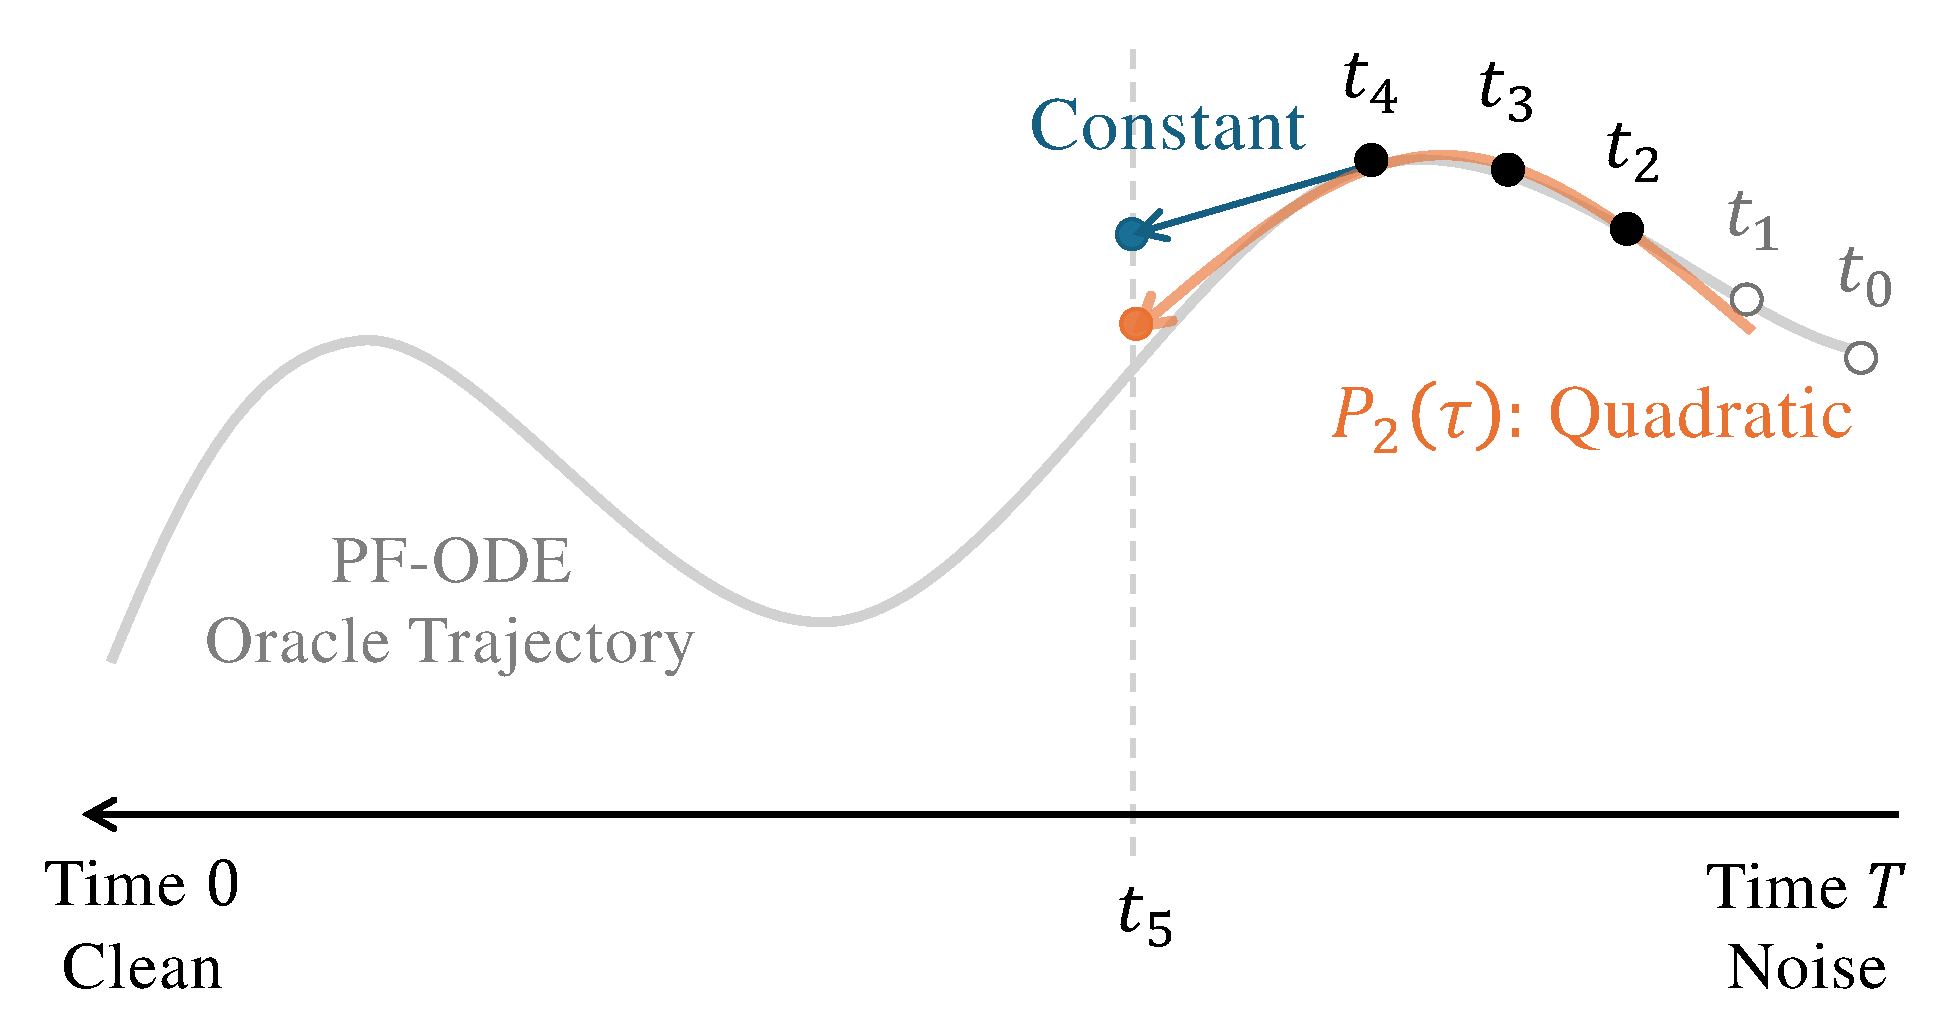
\includegraphics[width=\linewidth]{Images/PartC/DEIS.pdf}
    \caption{\textbfs{将 DEIS 视为多步方法的示意图。} 借助
$t_2,t_3,t_4$ 处的三个过去锚点，DEIS 通过模型输出构造一条二次曲线，
并对其解析积分以从
$t_4$ 步进到 $t_5$（外推）。这种高阶更新相比
DDIM 等一阶方法（仅使用 $t_4$ 处的值作积分的常数近似）减少了离散化误差。
\figcredit{由作者绘制。}}
    \label{fig:deis_lagrange}
\end{figure}

$n$ 次更新需要 $n{+}1$ 个锚点。当它们可用时（\emph{历史充分}，$i \ge n{+}1$），我们使用完整的 $n$ 次格式。在早期步骤中（\emph{历史不足}，$i \le n$），我们在可实现的最高次数 $i{-}1$ 上应用相同的构造，并随着更多锚点的累积而提高次数。下面我们依次处理这两种情形。



\paragraph{情形一：$i = n+1,\dots,M$（历史充分）。}
DEIS 不只依赖最近的估计
$\bm{\epsilon}_{\bm{\phi}^\times}(\tilde{\rvx}_{t_{i-1}},t_{i-1})$，
而是复用最后 $n{+}1$ 次模型求值作为锚点，
\[
(\tau_j,\rmY_j) := \bigl(t_{i-1-j}, \bm{\epsilon}_{\bm{\phi}^\times}(\tilde{\rvx}_{t_{i-1-j}},t_{i-1-j})\bigr),
\quad j=0,\dots,n.
\]
作为锚点。把 $\tau\mapsto\bm{\epsilon}_{\bm{\phi}^\times}(\rvx_\tau,\tau)$ 视为沿轨迹的光滑时间函数，我们构造 $n$ 次多项式（Lagrange 插值）
\[
P_n(\tau)
= 
\sum_{j=0}^{n}
\underbrace{\Bigl[\prod_{\substack{k=0\\k\neq j}}^{n}
\frac{\tau - t_{i-1-k}}{\,t_{i-1-j} - t_{i-1-k}\,}\Bigr]}_{=:~\ell_j^{(i)}(\tau)}
\bm{\epsilon}_{\bm{\phi}^\times}\bigl(\tilde{\mathbf x}_{t_{i-1-j}}, t_{i-1-j}\bigr)
\]
按构造它对每个锚点满足 $P_n(\tau_j)=\rmY_j$：
\[
P_n\bigl(\tau_j\bigr)
= \rmY_j =
\bm{\epsilon}_{\bm{\phi}^\times}\bigl(\tilde{\mathbf x}_{t_{i-1-j}}, t_{i-1-j}\bigr),
\quad
 j=0,\ldots,n.
\]
每个 $\ell_j^{(i)}$ 满足
\[
\ell_j^{(i)}\bigl(t_{i-1-m}\bigr)
=
\begin{cases}
1,&m=j,\\
0,&m\neq j.
\end{cases}
\]

Lagrange 多项式在新步上提供光滑外推：
\[
\bm{\epsilon}_{\bm{\phi}^\times}(\rvx_\tau,\tau) \approx
P_n(\tau)=\sum_{j=0}^{n}\ell_j^{(i)}(\tau) 
\bm{\epsilon}_{\bm{\phi}^\times}\bigl(\tilde{\rvx}_{t_{i-1-j}}, t_{i-1-j}\bigr), 
\quad \tau \in [t_{i-1},t_i].
\]
然后我们将 $P_r(\tau)$ 代入
指数积分器公式（\Cref{eq:variation_of_constants}）中 $\beps_{\bm{\phi}^\times}(\rvx_\tau,\tau)$ 的位置：
\begin{align*}
    \int_{t_{i-1}}^{t_i}
\frac{g^2(\tau)}{2 \sigma_\tau} 
\mathcal{E}&(\tau\to t_i) 
\beps_{\bm{\phi}^\times}(\rvx_\tau,\tau)\diff\tau
\\&\approx\sum_{j=0}^{r}
\underbrace{\int_{t_{i-1}}^{t_i}
\frac{g^2(\tau)}{2 \sigma_\tau} 
\mathcal{E}(\tau\to t_i) 
\ell_j^{(i)}(\tau)\diff\tau}_{=:~C_{i,j}} 
\beps_{\bm{\phi}^\times}(\tilde{\rvx}_{t_{i-1-j}},t_{i-1-j}).
\end{align*}
权重 $C_{i,j}$ 由
\begin{equation*}
C_{i,j} := \frac{1}{2} \int_{t_{i-1}}^{t_i} \frac{g^2(\tau)}{\sigma_\tau} \mathcal{E}(\tau \to t_i) \ell_j^{(i)}(\tau) \diff\tau,
\end{equation*}
给出，仅依赖于调度 $(\alpha_\tau,\sigma_\tau)$ 和网格
$\{t_i\}$。因此，一旦步长固定，它们就可以闭式地精确预计算。

用 $\mathcal{E}(t_{i-1}\to t_i)$ 精确积分线性部分，得到 \emph{AB-DEIS-$r$} 更新规则\footnote{“AB”指经典的
Adams–Bashforth 家族与指数时间差分多步方法~\citep{hochbruck2010exponential}。}，
\[
\tilde{\rvx}_{t_i}
=
\mathcal{E}(t_{i-1}\to t_i) \tilde{\rvx}_{t_{i-1}}
+
\sum_{j=0}^{r} C_{i,j} 
\beps_{\bm{\phi}^\times}(\tilde{\rvx}_{t_{i-1-j}},t_{i-1-j}).
\]
它在标准光滑性假设下给出 $r{+}1$ 阶的局部截断
误差.




\paragraph{情形二：$i=1,\dots,n$（历史不足）。}
对最初的若干步，只有 $i$ 个过去的点可用。因此我们把次数设为 $i{-}1$，并定义
\[
P_{i-1}(\tau)
=
\sum_{j=0}^{i-1}
\ell_j^{(i)}(\tau) 
\bm{\epsilon}_{\bm{\phi}^\times}\bigl(\tilde{\mathbf x}_{t_{i-1-j}},  t_{i-1-j}\bigr),
\]
其中 $\ell_j^{(i)}$ 是建立在时刻
$\{t_{i-1}, t_{i-2},\ldots,t_{0}\}$ 节点上的 $i{-}1$ 次 Lagrange 基。这匹配所有可用锚点，
并在 $i\ge n{+}1$ 时无缝过渡到完整历史公式。

这是多步求解器中标准的“热启动”。当历史较短时，我们拟合数据所允许的最丰富多项式：有一个锚点（$i{=}1$）时用 $0$ 次（常数）；有两个锚点（$i{=}2$）时用 $1$ 次（线性）；有三个锚点（$i{=}3$）时用 $2$ 次（二次）；以此类推，直到达到目标次数 $n$。实际上，随着更多历史可用，我们从单步预测逐步过渡到真正的 $(n{+}1)$ 步预测。


\exm{Lagrange 多项式的特例}{
\noindent \textbfs{当 $r=0$（一个锚点）：}
\[
P_0(\tau) = \bm{\epsilon}_{\bm{\phi}^\times}(\tilde\rvx_{t_{i-1}}, t_{i-1}).
\]
这只使用最近的值，因此近似在 $\tau$ 上是平坦的。
它对应于被积函数的左端点。

\medskip
\noindent \textbfs{当 $r=1$（两个锚点）：}Lagrange 多项式是穿过两个预先指定锚点的线性映射。
\[
P_1(\tau)
= 
\underbrace{\frac{\tau - t_{i-2}}{t_{i-1} - t_{i-2}}}_{\displaystyle \ell_{i-1}(\tau)}
\,\bm{\epsilon}_{\bm{\phi}^\times}(\tilde\rvx_{t_{i-1}}, t_{i-1})
 + 
\underbrace{\frac{\tau - t_{i-1}}{t_{i-2} - t_{i-1}}}_{\displaystyle \ell_{i-2}(\tau)}
\,\bm{\epsilon}_{\bm{\phi}^\times}(\tilde\rvx_{t_{i-2}}, t_{i-2}).
\]
这里 $\ell_{i-1}(\tau)$ 和 $\ell_{i-2}(\tau)$ 是 Lagrange 基权重。
它们满足插值（节点）条件
$P_1(t_{i-1})=\bm{\epsilon}_{\bm{\phi}^\times}(\tilde\rvx_{t_{i-1}}, t_{i-1})$ 与
$P_1(t_{i-2})=\bm{\epsilon}_{\bm{\phi}^\times}(\tilde\rvx_{t_{i-2}}, t_{i-2})$，
并且
$\ell_{i-1}(\tau)+\ell_{i-2}(\tau)=1$。
}

\paragraph{AB-DEIS-$n$ 更新总结。}
将历史充分与热启动（历史不足）两种情形合并，得到
\emph{AB-DEIS-$n$} 更新\footnote{“AB”指 Adams–Bashforth 家族的指数
时间差分多步方法~\citep{hochbruck2010exponential}。}，其中 $n$ 为多项式
次数（最多使用 $n{+}1$ 次过去的求值），如下：
\begin{mdframed}
\begin{align*}
\tilde\rvx_{t_i}
= \mathcal{E}(t_{i-1} \to t_i)\,\tilde\rvx_{t_{i-1}}
+ \sum_{j=0}^{\min\{n,\, i-1\}} C_{i,j}\,\beps_{\bm{\phi}^\times}(\tilde\rvx_{t_{i-1-j}},\,t_{i-1-j}),
\end{align*}
系数为
\begin{align*}
C_{i,j}
:= \frac{1}{2} \int_{t_{i-1}}^{t_i}
\frac{g^2(\tau)}{\sigma_\tau}\,\mathcal{E}(\tau \to t_i)\,
\Bigg[\prod_{\substack{k=0\\k\neq j}}^{\min\{n,\, i-1\}}
\frac{\tau - t_{i-1-k}}{\,t_{i-1-j} - t_{i-1-k}\,}\Bigg]\,d\tau.
\end{align*}
\end{mdframed}

当 $i\ge n{+}1$（历史充分）时，$\min\{n,\, i-1\}=n$
，在标准光滑性假设下该步达到局部截断误差 $\mathcal O(h^{\,n+1})$。
在热启动期间（$i\le n$），$\min\{n,\, i-1\}=i-1$，每步阶数为 $\mathcal O(h^{\,\min\{n,\, i-1\}+1})$，逐步爬升
直到达到完整阶数。

然而，非常大的 $n$ 往往由于插值病态、噪声放大以及更严格的稳定性约束而损害性能；小次数（例如 $n \in \{1,2,3\}$）通常提供最佳的精度—稳定性折中。

正如下一小节将看到的，$n{=}0$ 的特殊情形退化为指数 Euler/DDIM。



\subsection{DDIM = AB-DEIS-0}\label{sec:ddim-deis} 我们观察到，当 $ n = 0 $（即常数多项式）时，系数简化为：
\[
C_{i0} = \frac{1}{2} \int_{t_{i-1}}^{t_{i}} \frac{g^2(\tau)}{\sigma_\tau} \mathcal{E}(\tau \shortrightarrow t_i)   \mathrm{d}\tau.
\]
代入更新公式得到零阶 AB-DEIS 格式：
\begin{align}\label{eq:deis-0}
  \tilde\rvx_{t_{i}} &=  \mathcal{E}(t_{i-1} \shortrightarrow t_{i})\tilde\rvx_{t_{i-1}} + C_{i0} \bm{\epsilon}_{\bm{\phi}^\times}(\tilde\rvx_{t_{i-1}}, t_{i-1})\nonumber\\
  &=e^{\int_{t_{i-1}}^{t_{i}}f(u)\diff u} \tilde\rvx_{t_{i-1}} + \Big( \int_{t_{i-1}}^{t_{i}} \frac{g^2(\tau)}{2\sigma_\tau} e^{\int_{\tau}^{t_{i}}f(u)\diff u}   \mathrm{d}\tau
\Big) \bm{\epsilon}_{\bm{\phi}^\times}(\tilde\rvx_{t_{i-1}}, t_{i-1}).  
\end{align}
这正是指数 Euler 步（$[t_{i-1},t_i]$ 上 $\beps_{\bphi^\times}$ 为时间常数），与
确定性 DDIM 更新一致。我们在下面正式陈述这一对应关系。
\proppnp{DDIM = AB-DEIS-0}{ddim-deis}{\Cref{eq:deis-0} 与 \Cref{eq:ddim-euler} 中的 DDIM 更新完全相同。}


    
\clearpage
\newpage



\section{\texorpdfstring{DPM-Solver}{DPM-Solver}}\label{sec:dpm}

DPM-Solver 家族，包括 DPM-Solver~\citep{lu2022dpm}、DPM-Solver\texttt{++}~\citep{lu2022dpm2} 和 DPM-Solver-v3~\citep{zheng2023dpm}，代表了 PF-ODE 求解器的一项重大进展。其目标很简单：以远更少的步数达到相当的样本质量。在实践中，这些方法把 DDIM 所需的步数从 $50$ 多步减少到约 $10$--$15$ 步，使生成更高效。此外，DPM-Solver\texttt{++} 和 DPM-Solver-v3 设计用于处理条件生成中的无分类器引导（CFG）（见 \Cref{sec:cfg}）。本节首先讲解核心的 DPM-Solver~\citep{lu2022dpm}；其扩展见 \Cref{sec:dpm++}。

\paragraph{DPM-Solver 的高层思想。}
与 DEIS 一样，DPM-Solver 从 PF-ODE 的半线性形式出发，在 $\beps$-预测参数化下工作，使用 \Cref{eq:exp-int-factor} 中的指数积分器（常数变易）表示：
\begin{align}\label{eq:noise-alpha-sigma}
    \frac{\diff \rvx_t}{\diff t}
= \frac{\alpha_t'}{\alpha_t}\rvx_t
- \sigma_t \left(\frac{\alpha_t'}{\alpha_t}-\frac{\sigma_t'}{\sigma_t}\right)
\beps_{\bphi^\times}(\rvx_t,t).
\end{align}
关键思想是用半对数信噪比重新参数化时间，使指数积分器公式中的非线性项变为一个指数加权的积分。这种表示允许在 $\lambda$ 中进行低成本的 Taylor 展开，自然地给出高阶更新规则。我们随后将直观解释为何这种重参数化有效。



\subsection{DPM-Solver 的洞见：通过 log-SNR 进行时间重参数化}\label{subsec:dpm-method}   
在半线性结构之上，DPM-Solver 的一个关键洞见是：标准的时间参数化 $t$ 对扩散模型的数值积分而言是次优的。他们转而提出用\emph{半对数信噪比}（half-log SNR）
\begin{align}\label{eq:lambda}
    \lambda_t \coloneqq \frac{1}{2}\log \frac{\alpha_t^2}{\sigma_t^2}  =  \log \frac{\alpha_t}{\sigma_t},
\end{align}
来重参数化时间，
沿用 VDM~\citep{kingma2021variational} 的 log-SNR 参数化。
这种换元简化了非线性被积函数，从而能够进行更易处理、更精确的高阶模型估计。






\paragraph{将 PF-ODE 换元到 log-SNR。} 现在我们用半对数 log-SNR $\lambda_t := \log(\alpha_t/\sigma_t)$ 重新参数化时间。
对常见的噪声调度，$\lambda_t$ 关于 $t$ 严格递减。在此假设下，它有反函数 $t_\lambda(\cdot)$ 把 $\lambda$ 映射到 $t$，满足
\[
t = t_\lambda(\lambda(t)).
\]
然后我们将 $\rvx$ 和 $\bm{\epsilon}_{\bm{\phi}^\times}$ 的下标由 $t$ 改为 $\lambda$。带帽子（  $\hat{\cdot}$  ）表示该量以 $\lambda$ 表示。更精确地，定义：
\begin{align}
\begin{aligned}
    \label{eq:change-of-var-x-epsilon}
 \hat{\rvx}_{\lambda} & := \rvx_{t_\lambda(\lambda)}, \\
 \hat{\bm{\epsilon}}_{\bm{\phi}^\times}(\hat{\rvx}_{\lambda}, \lambda) & \coloneqq \bm{\epsilon}_{\bm{\phi}^\times}(\rvx_{t_\lambda(\lambda)}, t_\lambda(\lambda)).
\end{aligned}
\end{align}

通过从 $t$ 到 $\lambda_t$ 的换元，\Cref{eq:noise-alpha-sigma} 中 PF-ODE 的精确解 $\widetilde\bPsi_{s\to t}$ 变为：
\proppp{指数加权的精确解}{exp-wgt-exact-sol}{给定时刻 $s>0$ 的初值 $\rvx_s$，PF-ODE 在时刻 $t\in[0,s]$ 的精确解 $\widetilde\bPsi_{s\to t}(\rvx_s)$ 可以重新表示为：
\begin{equation}
\label{eq:analytic_solution}
    \widetilde\bPsi_{s\to t}(\rvx_s) = \frac{\alpha_t}{\alpha_s}\rvx_s - \alpha_t \int_{\lambda_s}^{\lambda_t} e^{-\lambda} \hat{\bm{\epsilon}}_{\bm{\phi}^\times}(\hat\rvx_\lambda,\lambda)\diff \lambda.
\end{equation}}{虽然可以直接对 \Cref{eq:noise-alpha-sigma} 施加换元得到结果，但为了清晰与完整，下面给出另一种推导。
利用关系 $ g^2(t) = -2\sigma_t^2\frac{\diff \lambda_t}{\diff t} $，\Cref{eq:noise-alpha-sigma} 可改写为：
\[
\frac{\diff \rvx_t}{\diff t} = \frac{\diff \log \alpha_t}{\diff t} \rvx_t - \sigma_t \frac{\diff \lambda_t}{\diff t} \bm{\epsilon}_{\bm{\phi}^\times}(\rvx_t, t).
\]
应用链式法则：
\[
\frac{\diff \rvx_t}{\diff t} = \frac{\diff \hat\rvx_\lambda}{\diff \lambda} \frac{\diff \lambda_t}{\diff t} \quad \text{and} \quad \frac{\diff \log\alpha_t}{\diff t} = \frac{\diff \log\alpha_\lambda}{\diff \lambda} \frac{\diff \lambda_t}{\diff t},
\]
$t $ 中的 ODE 变换为 $ \lambda $ 中的 ODE：
\begin{align*}
    \frac{\diff \hat\rvx_\lambda}{\diff \lambda} &= \Big(\frac{\diff \lambda_t}{\diff t}\Big)^{-1} \frac{\diff \rvx_t}{\diff t} \\
    &= \Big(\frac{\diff \lambda_t}{\diff t}\Big)^{-1} \Big[ \frac{\diff \log \alpha_t}{\diff t} \rvx_t - \sigma_t \frac{\diff \lambda_t}{\diff t} \bm{\epsilon}_{\bm{\phi}^\times}(\rvx_t, t) \Big] \\
    &= \Big(\frac{\diff \lambda_t}{\diff t}\Big)^{-1} \Big[ \frac{\diff \log\alpha_\lambda}{\diff \lambda} \frac{\diff \lambda_t}{\diff t} \hat\rvx_\lambda - \sigma_\lambda \frac{\diff \lambda_t}{\diff t} \hat{\bm{\epsilon}}_{\bm{\phi}^\times}(\hat\rvx_\lambda, \lambda) \Big] \\
    &= \frac{\diff \log\alpha_\lambda}{\diff \lambda} \hat\rvx_\lambda - \sigma_\lambda \hat{\bm{\epsilon}}_{\bm{\phi}^\times}(\hat\rvx_\lambda, \lambda).
\end{align*}
于是，变换后的 ODE 变为 \Cref{eq:diffusion_ode_lambda_eps}。然后我们可对 \Cref{eq:diffusion_ode_lambda_eps} 施加同样的“指数积分器（EI）”技术来推导 \Cref{eq:analytic_solution}。
}

在 $\lambda$--时间下，模型出现在一个指数加权的积分中，
\[
\int_{\lambda_s}^{\lambda_t} e^{-\lambda} \hat{\bm{\epsilon}}_{\bm{\phi}^\times}(\hat\rvx_\lambda,\lambda) \diff \lambda,
\]
其中 $e^{-\lambda}$ 因子产生闭式系数并使被积函数变平滑，这正是高阶局部近似所需要的。

等价地，从 $t$ 到 $\lambda$ 的换元把 PF-ODE 变换为如下的微分形式（见上一命题中的推导）：
\begin{mdframed}
\begin{align}\label{eq:diffusion_ode_lambda_eps}
\frac{\diff \hat{\rvx}_\lambda}{\diff \lambda}
= \frac{\alpha_\lambda'}{\alpha_\lambda} \hat{\rvx}_\lambda
- \sigma_\lambda \hat{\bm{\epsilon}}_{\bm{\phi}^\times}(\hat{\rvx}_\lambda, \lambda).
\end{align}
\end{mdframed}


\paragraph{为何要重参数化时间的直观理解？}
对严格单调的 $\lambda(t)$，一阶换元给出
\[
\Delta t  \approx  \frac{\Delta\lambda}{ |\lambda'(t)| }.
\]
因此，对固定的 $\Delta\lambda$，所诱导的 $\Delta t$ 在 $|\lambda'(t)|$ 较大处（即 $\lambda$ 随 $t$ 快速变化处）更小，在 $|\lambda'(t)|$ 较小处更大。
这种重参数化并不改变 PF--ODE 的解路径，只改变速度：
\[
\frac{\diff \hat\rvx_\lambda}{\diff \lambda}
= \frac{1}{\lambda'(t)} \frac{\diff \rvx_t}{\diff t}.
\]
于是，在 $|\lambda'(t)|$ 大的区域，$\lambda$--域导数被 $1/|\lambda'(t)|$ 缩放，往往使被积函数在均匀 $\lambda$ 网格上更平滑。
（大 $|\lambda'(t)|$ 的精确位置取决于所选调度。）

从概念上讲，我们可能希望在过程接近复杂（数据）分布时分配更多的时间步。下面两个简单的调度示例说明了这种效应：
\begin{itemize}
\item $(\alpha_t,\sigma_t)=(1-t, t)$：这对应 FM 调度器。则
\[
\lambda(t)=\log\frac{1-t}{t},\quad 
\lambda'(t)=-\frac{1}{t(1-t)},\quad
\Delta t \approx \Delta\lambda   t(1-t).
\]
因此步长在两端（$t\to 0,1$）附近很小，在中间时刻附近最大。

\item $(\alpha_t,\sigma_t)=(1, t)$：这是 EDM 调度器~\citep{karras2022elucidating}，在 \Cref{sec:edm} 中介绍。若直接取自变量为噪声水平 $t=\sigma_t$，则
\[
\lambda(t)=\log\frac{1}{t},\quad 
\lambda'(t)=-\frac{1}{t},\quad
\Delta t \approx \Delta\lambda   t.
\]
$\lambda$ 中的均匀间距对应 $t$ 中的几何间距，或等价地对应方差中的几何间距（在小 $t$/高 SNR 处有大量小步，在大 $t$ 处更粗糙）。
\end{itemize}




\subsection{用 Taylor 展开估计积分}\label{subsec:dpm-method-2} 
DEIS 通过对跨先前求值的被积函数作多项式
插值来近似该指数加权积分（一种多步
方法）。DPM-Solver 从相同的精确积分表述出发，
但用 log-SNR 变量~$\lambda$ 重参数化时间，并通过在~$\lambda$ 中的局部 Taylor 展开（在每步内使用中间分阶段的求值）来导出
高阶更新（一种单步
方法）。后续的 DPM-Solver 多步变体与 DEIS 基于插值的视角联系更紧密，我们将在 \Cref{sec:summary-solver} 中回到这一比较。现在我们给出 DPM-Solver 的单步推导。



由 \Cref{eq:analytic_solution}，从时刻 $s$ 的前一个点 $\tilde\rvx_{s}$ 出发，时刻 $t$ 的解 $\tilde\rvx_{t} $ 为
\begin{equation}
\label{eqn:analytic_solution_each_step}
    \tilde\rvx_{t}  = \frac{\alpha_{t}}{\alpha_{s}} \tilde\rvx_{s} - \alpha_{t} \int_{\lambda_{s}}^{\lambda_{t}} e^{-\lambda} \hat{\bm{\epsilon}}_{\bm{\phi}^\times}(\hat\rvx_{\lambda}, \lambda)\diff\lambda.
\end{equation}
因此，我们需要近似如下形式的积分：
\begin{align*}
    \int_{\lambda_{s}}^{\lambda_{t}} e^{-\lambda} \hat{\bm{\epsilon}}_{\bm{\phi}^\times}(\hat\rvx_{\lambda}, \lambda)\diff\lambda.
\end{align*}

在区间 $\lambda \in [\lambda_{s}, \lambda_{t_i}]$ 上，我们对 \Cref{eqn:analytic_solution_each_step} 中的被积函数 $\hat{\bm{\epsilon}}_{\bm{\phi}^\times}(\hat\rvx_\lambda, \lambda)$ 用关于 $\lambda$ 的 Taylor 展开来近似。对 $n \geq 1$，关于 $\lambda_{s}$ 的 $(n{-}1)$ 阶 Taylor 展开为
\begin{equation*}
    \hat{\bm{\epsilon}}_{\bm{\phi}^\times}(\hat\rvx_\lambda, \lambda)
    = \sum_{k=0}^{n-1} \frac{(\lambda - \lambda_{s})^k}{k!} 
    \hat{\bm{\epsilon}}_{\bm{\phi}^\times}^{(k)}(\hat\rvx_{\lambda_{s}}, \lambda_{s})
    + \mathcal{O}((\lambda - \lambda_{s})^n),
\end{equation*}
其中关于 $\lambda$ 的 $k$ 阶全导数记为
\[
\hat{\bm{\epsilon}}_{\bm{\phi}^\times}^{(k)}(\hat\rvx_\lambda, \lambda) 
\coloneqq \frac{\diff^k}{\diff\lambda^k} \hat{\bm{\epsilon}}_{\bm{\phi}^\times}(\hat\rvx_\lambda, \lambda).
\]

将此展开代入 \Cref{eqn:analytic_solution_each_step} 中的积分，得到一个闭式近似，它定义了 $n$ 阶求解器，称为 \emph{DPM-Solver-$n$}。

\begin{mdframed}
从前一步的估计 $\tilde\rvx_{s}$ 出发，
\begin{equation}
    \label{eq:k-th-expansion}
    \tilde\rvx_{t}  =  \frac{\alpha_{t}}{\alpha_{s}} \tilde\rvx_{s} - \alpha_{t} \sum_{k=0}^{n-1} {\color{cyan}\hat{\bm{\epsilon}}_{\bm{\phi}^\times}^{(k)}(\hat\rvx_{\lambda_{s}},\lambda_{s})} ~{\color{orange}C_k}  + \mathcal{O}(h^{n+1}),
\end{equation}
这里记 $h\coloneqq \lambda_{t} - \lambda_{s}$，并定义：
\begin{align*}
    {\color{orange}C_k}\coloneqq\int_{\lambda_{s}}^{\lambda_{t}}   e^{-\lambda}  \frac{(\lambda - \lambda_{s})^k}{k!}\diff\lambda.
\end{align*}
${\color{orange}C_k}$ 可通过应用 $k$ 次分部积分解析地预计算。
\end{mdframed}
我们注意到，换元 $t \mapsto \lambda$ 用于
平滑被积函数并推导系数，而求解器
返回的是 $t$-网格上的估计 $\tilde{\rvx}_{t}$。

下面，我们以 DPM-Solver-1 为例说明。


\exm{DPM-Solver-1}{
为演示取 $n=1$（一阶）。从前一个估计点 $\tilde\rvx_{s}$ 出发，\Cref{eq:k-th-expansion} 简化为：
\begin{align}\label{eq:dpm-1}
    \tilde\rvx_{t} &= \frac{\alpha_{t}}{\alpha_{s}} \tilde\rvx_{s} - \alpha_{t} \bm{\epsilon}_{\bm{\phi}^\times}(\tilde\rvx_{s},s) \int_{\lambda_{s}}^{\lambda_{t}} e^{-\lambda}\diff\lambda + \mathcal{O}(h^2) \nonumber \\
    &= \frac{\alpha_{t}}{\alpha_{s}} \tilde\rvx_{s} - \sigma_{t} (e^{h} - 1)\bm{\epsilon}_{\bm{\phi}^\times}(\tilde\rvx_{s},s) + \mathcal{O}(h^2).   
    \end{align}
上式正是 DDIM 更新；我们在 Proposition~\ref{ddim-dpm} 中证明其等价性。
}

$n \ge 2$ 的 DPM-Solver-$n$ 需要对 $k \le n-1$ 求值 $k^{\text{th}}$ 阶导数 {\color{cyan}$\hat{\bm{\epsilon}}_{\bm{\phi}^\times}^{(k)}(\hat\rvx_\lambda, \lambda)$}。然而，在实践中直接计算高阶导数代价高昂。\citet{lu2022dpm} 也提出了这些导数的高效近似方法，将在下一小节详述。

 
\subsection{DPM-Solver-$n$ 的实现}\label{subsec:dpm-n-method} 

\paragraph{$n \ge 2$ 的 DPM-Solver-$n$。}
在实践中，实现高阶的 DPM-Solver-$n$ 包含以下内容：
\begin{itemize}
    \item 预计算系数 ${\color{orange}C_k}$；
    \item 近似 $k \le n-1$ 的 $k^{\text{th}}$ 阶导数 {\color{cyan}$\hat{\bm{\epsilon}}_{\bm{\phi}^\times}^{(k)}(\hat\rvx_\lambda,\lambda)$} 以规避昂贵的精确高阶导数计算——这是 ODE 文献中研究充分的一个挑战~\citep{hochbruck2005explicit,luan2021efficient}。一种常见策略是有限差分近似。
\end{itemize}

下面我们详细说明前两点。


\subparagraph{预计算 ${\color{orange}C_k}$。} 
设 $s$ 和 $t$ 分别表示起始和终止时刻，并定义 $h := \lambda_t - \lambda_s$。从 $\rvx_s$ 出发，\Cref{eq:variation_of_constants} 的精确解的解析展开为：
\begin{equation}
\label{eq:analytic_expansion}
    \rvx_{t} = \frac{\alpha_{t}}{\alpha_{s}}\rvx_{s} - \sigma_{t} \sum_{k=0}^{n-1} h^{k+1} \varphi_{k+1}(h) \hat{\bm{\epsilon}}_{\bm{\phi}^\times}^{(k)}(\hat\rvx_{\lambda_{s}}, \lambda_{s}) + \mathcal{O}(h^{n+1}),
\end{equation}
其中每个 $\varphi_{k+1}(\cdot)$ 有闭式表达。对 $k = 0, 1, 2$，它们为：
\begin{align*}
\varphi_1(h) &= \frac{e^h - 1}{h}, &
\varphi_2(h) &= \frac{e^h - h - 1}{h^2}, &
\varphi_3(h) &= \frac{e^h - \frac{h^2}{2} - h - 1}{h^3}.
\end{align*}

\exm{使用精确导数的 DPM-Solver-2/3}{对 $n = 3$ 及离散时间步 $h := \lambda_{t} - \lambda_{s}$，展开变为：
\begin{equation}\label{eq:example-dpm-solver-3-exact}
\begin{aligned}
    \rvx_{t} = \frac{\alpha_{t}}{\alpha_{s}} \rvx_{s}
    &- \sigma_{t} \left(e^{h} - 1\right) \hat{\bm{\epsilon}}_{\bm{\phi}^\times}(\hat\rvx_{\lambda_{s}}, \lambda_{s}) \\
    &- \sigma_{t} \left(e^{h} - h - 1\right) \hat{\bm{\epsilon}}_{\bm{\phi}^\times}^{(1)}(\hat\rvx_{\lambda_{s}}, \lambda_{s}) \\
    &- \sigma_{t} \left(e^{h} - \frac{h^2}{2} - h - 1\right) \hat{\bm{\epsilon}}_{\bm{\phi}^\times}^{(2)}(\hat\rvx_{\lambda_{s}}, \lambda_{s}) \\
    &+ \mathcal{O}(h^4).
\end{aligned}
\end{equation}}





\subparagraph{近似 $k \le n-1$ 的 {\color{cyan}$\hat{\bm{\epsilon}}_{\bm{\phi}^\times}^{(k)}(\hat\rvx_\lambda,\lambda)$}。}
对 $n \ge 2$，遵循单步 ODE 求解器的标准方法~\citep{atkinson2009numerical}，\citet{lu2022dpm} 在 $s$ 和 $t$ 之间引入中间时间步 $s^{\mathrm{mid}}$，用 $s$ 和 $s^{\mathrm{mid}}$ 处的函数求值来近似高阶导数。我们以 $n = 2$ 的情形为例说明。

设 $\gamma \in (0,1]$ 为指定 log-SNR 区间 $[\lambda_s, \lambda_t]$ 内一个插值点的超参数。
给定 $s$ 处的估计 $\tilde\rvx_s$，定义
\[
    s^{\mathrm{mid}} = t_\lambda\left(\lambda_s + \gamma h\right), \quad \text{where } h := \lambda_t - \lambda_s,
\]
中间估计由下式给出：
\[
    \rvx^{\mathrm{mid}} = \frac{\alpha_{s^{\mathrm{mid}}}}{\alpha_s} \tilde\rvx_s - \sigma_{s^{\mathrm{mid}}} \left(e^{\gamma h} - 1\right) \bm{\epsilon}_{\bm{\phi}^\times}(\tilde\rvx_s, s).
\]
这给出如下二阶近似：
\begin{align}
\label{eq:dpm-solver-2-app}
\begin{aligned}
    \tilde{\rvx}_{t} = \frac{\alpha_{t}}{\alpha_s} \tilde\rvx_s 
    &- \sigma_{t} \left(e^{h} - 1\right) \bm{\epsilon}_{\bm{\phi}^\times}(\tilde\rvx_s, s) \\
    &- \frac{\sigma_t}{\gamma h} \left(e^{h} - h - 1\right) \left( \bm{\epsilon}_{\bm{\phi}^\times}(\rvx^{\mathrm{mid}}, s^{\mathrm{mid}}) - \bm{\epsilon}_{\bm{\phi}^\times}(\tilde\rvx_s, s) \right)
     +  \mathcal{O}(h^3).
\end{aligned}
\end{align}


取 $\gamma=\tfrac12$ 时，\Cref{alg:dpm-solver-2} 中的两阶段更新在相差 $\mathcal O(h^3)$（局部截断误差）的意义下等价于
\Cref{eq:dpm-solver-2-app}。
\begin{algorithm}[H]
    \centering
    \caption{DPM-Solver-2（取 $\gamma=\tfrac12$）。}\label{alg:dpm-solver-2}
    \begin{algorithmic}[1]
    \Require 初值 $\rvx_T$，时间步 $\{t_i\}_{i=0}^M$，模型 ${\bm{\epsilon}}_{\bm{\phi}^\times}$
        \State $\tilde\rvx_{t_0}\gets\rvx_T$
        \For{$i\gets 1$ to $M$}
        \State $h_i \gets \lambda_{t_i} - \lambda_{t_{i-1}}$
        \State $s_{i}^{\text{mid}} \gets t_{\lambda}\left(\tfrac{\lambda_{t_{i-1}} + \lambda_{t_i}}{2}\right)$
        \State 
    $\rvx_{i}^{\text{mid}} \gets \tfrac{\alpha_{s_i^{\text{mid}}}}{\alpha_{t_{i-1}}} \tilde\rvx_{t_{i-1}} - \sigma_{s_i^{\text{mid}}}\left(e^{\tfrac{h_i}{2}} - 1\right){\bm{\epsilon}}_{\bm{\phi}^\times}(\tilde \rvx_{t_{i-1}},t_{i-1})$ 
    \State  $\tilde\rvx_{t_{i}} \gets \tfrac{\alpha_{t_{i}}}{\alpha_{t_{i-1}}} \tilde\rvx_{t_{i-1}} - \sigma_{t_{i}}\left(e^{h_i} - 1\right){\bm{\epsilon}}_{\bm{\phi}^\times}(\rvx_{i}^{\text{mid}},s_i^{\text{mid}})$
        \EndFor
        \State \Return $\tilde\rvx_{t_M}$
    \end{algorithmic}
\end{algorithm}

\rmkb{
在 \Cref{eq:dpm-solver-2-app} 中，差商
\[
\hat{\bm{\epsilon}}_{\bm{\phi}^\times}^{(1)}(\hat\rvx_{\lambda_s},\lambda_s)
\approx
\frac{\bm{\epsilon}_{\bm{\phi}^\times}(\rvx^{\mathrm{mid}}, s^{\mathrm{mid}})
      - \bm{\epsilon}_{\bm{\phi}^\times}(\tilde\rvx_s, s)}{\gamma h}
\]
近似了模型沿轨迹的 $\lambda$ 全导数。
此近似精确到 $\mathcal O(h)$，而在 \Cref{eq:dpm-solver-2-app} 中它乘以了精确的 $\varphi_2$ 系数 $e^h-h-1=\mathcal O(h^2)$。
因此，所得贡献仅为 $\mathcal O(h^3)$，所以对任意 $\gamma \in (0,1]$ 整个格式都达到二阶精度。

每步恰好需要两次模型求值：一次在 $(\tilde\rvx_s,s)$，另一次在预测的中点 $(\rvx^{\mathrm{mid}},s^{\mathrm{mid}})$。
插值参数 $\gamma$ 不影响精度阶，但它改变误差常数：取 $\gamma=\tfrac12$ 会使模板对称化，通常能最小化常数，这也是实践中偏好中点版本的原因。

}


对 $n \ge 3$ 的高阶 DPM-Solver-$n$，采用类似的方法，利用中间时间步以有限差分方式近似高阶导数。详细方法见原始 DPM 论文。


对熟悉数值 ODE 求解器的读者，\textsc{DPM-Solver} 可以被视为半线性 PF-ODE 的单步\emph{指数积分器}，并结合了到（半）log--SNR 的时间变量替换。其二阶与三阶变体是指数 Runge--Kutta 型格式，在每步内使用少量分阶段的模型求值。


\paragraph{实现细节：采样时间步的选择。} 为进行采样，求解器必须首先预定义一时间步序列 $\{t_i\}_{i=0}^M$。
\citet{lu2022dpm} 提出基于在 log--SNR 时间 $\lambda_t$ 中\emph{均匀间距}来选择这些步，即
\[
\lambda_{t_i} = \lambda_T + \frac{i}{M}(\lambda_0 - \lambda_T), \quad i = 0, \dots, M.
\]
这不同于早前方法~\citep{ho2020denoising,song2020score} 直接在物理时间变量~$t$ 中使用均匀间距的做法。
经验上，DPM-Solver 在使用均匀 $\lambda$ 间距时，即使步数很少也能得到高质量样本\footnote{或者，自适应步长策略通过组合不同阶数的求解器来动态调整时间步；见 \citet{lu2022dpm} 的附录 C。}。

从概念上讲，这可以从几何角度理解：局部 Taylor 近似的精度取决于动力学在 $\lambda$ 中演化的光滑程度。
因此 $\lambda$ 中的均匀间距在轨迹上产生近似均匀的局部误差，使得在信号主导（高 SNR）处有更细（更密）的 $t$ 步，在噪声主导的情形下有更粗（更稀）的步。



虽然推导在 $\lambda$--空间中进行，且 PF--ODE 在该域中表述为方便的半线性形式，但预训练模型和噪声调度 $(\alpha_t, \sigma_t)$ 通常相对于原始时间变量 $t$ 定义。
在采样过程中，求解器为数值稳定性选取在 $\lambda$ 中均匀间距的节点，但所有更新方程都以 $t$ 表达。
每当需要求值模型或检索调度值时，所选的 $\lambda$ 节点被映射回相应的时间变量，如物理时间 $t = t_\lambda(\lambda)$ 或方差参数 $\sigma_t$，具体取决于模型的参数化方式（例如见 \Cref{alg:dpm-solver-2}）。








\subsection{DDIM $=$ DPM-Solver-1}\label{subsec:ddim=dpm-solver-1}
对固定的调度 $(\alpha_t,\sigma_t)$，DPM-Solver-1 步
与确定性 DDIM（$\eta=0$）更新一致，
与时间参数化（物理时间 $t$ 或 log--SNR 时间 $\lambda$）无关；
正式陈述见下。
\proppp{DDIM 即 DPM-Solver-1}{ddim-dpm}{
\Cref{eq:ddim-euler} 给出的 DDIM 更新规则，与 \Cref{eq:dpm-1} 给出的 DPM-Solver-1 更新规则相同。
}{
由 $\lambda$ 的定义，有
\begin{align}
    \frac{\sigma_s}{\alpha_s} = e^{-\lambda_s} \quad \text{and} \quad \frac{\sigma_t}{\alpha_t} = e^{-\lambda_t}.
\end{align}
将这些表达式连同 $h = \lambda_t - \lambda_s$ 代入 \Cref{eq:ddim-euler}，即恢复 \Cref{eq:dpm-1} 中的更新规则，完成等价性证明。
}
上述命题或许能解释为何 DDIM 优于 $t$-参数化下的传统 Euler 方法：它在更合适的 $\lambda$-重参数化下有效地利用了扩散 ODE 的半线性。


\rmkb{当 Score SDE 论文出现时，常用 Runge--Kutta（RK45）来求解 \Cref{eq:prob_ode_sub} 中的朴素 PF-ODE，但其漂移的半线性并未被利用。尽管 DPM-Solver-$k$（$k \geq 2$）与 Runge--Kutta 方法有关，但它通过时间重参数化明确地利用了这种半线性。这解释了为何 DPM-Solver 能以远更少的函数求值达到高阶精度，在保持高样本质量的同时把 DDIM 通常数百步的调度减少到约 $10$--$15$ 步。
}






\subsection{关于 DPM-Solver-2 与经典 Heun 更新的讨论}\label{subsec:dpm-heun}

在 \Cref{subsec:ddim-different-para} 中我们看到，PF--ODE 的不同参数化给出经典 Euler 型更新的不同解读：
\begin{align*}
\text{$\rvv$-prediction:} 
&\quad \text{Euler} = \text{DDIM}, \\[4pt]
\text{$\beps$-, $\rvx$-, or $\rvs$-prediction:} 
&\quad \text{exp--Euler} = \text{DDIM} \neq \text{plain Euler}.
\end{align*}

本小节我们进一步通过考察经典 \emph{Heun 方法}与二阶 DPM--Solver 在四种参数化下的类似关系来说明这一联系。


作为铺垫，我们简要回顾 Heun 方法（另见 \Cref{app:de-solver}）。
Heun 方法是一种二阶求解器，它通过预测器-校正器格式改进 Euler 方法：
它先做一次 Euler 预测到步的终点，在那里求值斜率，然后用
起点与预测斜率的平均进行更新。
直观上，它沿区间内的平均斜率前进
（梯形的面积），达到比朴素 Euler 高得多的精度。

我们在 log--SNR 时间 $\lambda$ 中工作，其中 PF--ODE 可表示为简单的“线性 + 非线性”形式：
\[
\frac{\diff \hat{\rvx}(\lambda)}{\diff \lambda}
= \underbrace{L(\lambda)\hat{\rvx}(\lambda)}_{\text{linear part}} + \underbrace{\rmN\big(\hat{\rvx}(\lambda),\lambda\big)}_{\text{nonlinear part}},
\]
其中标量 $L(\lambda)$ 由噪声调度决定，$\rmN(\cdot,\lambda)$ 收集非线性部分。
这种结构自然来自 \Cref{eq:clean_pf_ode}：$\beps$-、$\rvx$-和 $\rvs$-预测参数化给出非零 $L(\lambda)$，从而呈现半线性形式。
相比之下，$\rvv$-预测对应于 $L(\lambda)\equiv 0$（因此 $\rmN=\rvv$），不留下显式的线性项。


在下文的讨论中，我们先回顾不考虑任何半线性结构的朴素 Heun 更新，
然后引入指数 Heun 更新——它专为半线性 ODE 设计并精确处理线性部分，类似于 \Cref{eq:exp-euler-step,eq:euler-step} 中的指数 Euler 步。
最后，我们将两种 Heun 更新与四种参数化下的 DPM-Solver-2 联系起来，并得出结论：
\begin{align*}
\text{$\rvv$-prediction:} 
&\quad \text{Heun} = \text{DPM-Solver-2}, \\[4pt]
\text{$\beps$-, $\rvx$-, or $\rvs$-prediction:} 
&\quad \text{exp-Heun} = \text{DPM-Solver-2} \neq \text{plain Heun}.
\end{align*}

\begin{figure}[th!]
    \centering
    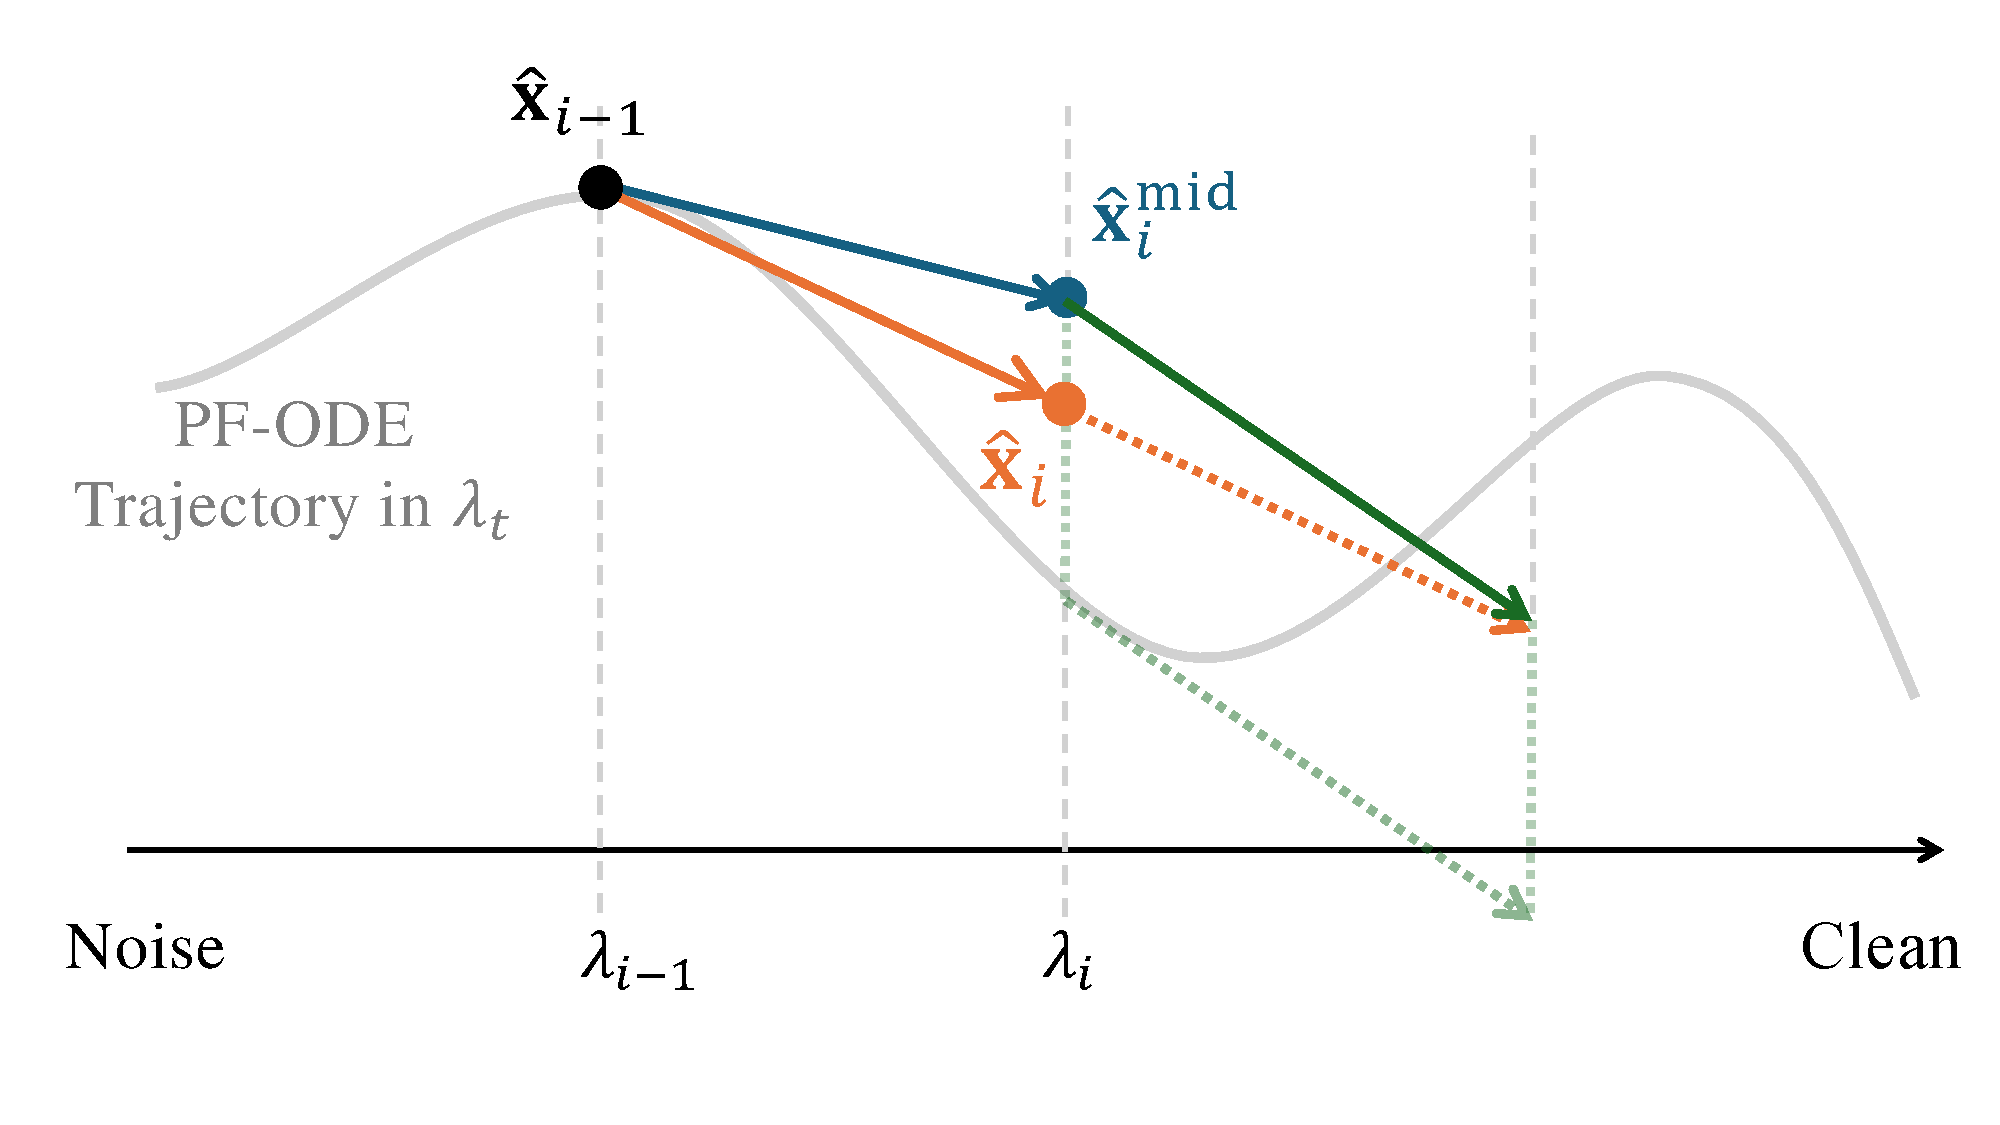
\includegraphics[width=\linewidth]{Images/PartC/Heun.pdf}
\caption{
\textbfs{log-SNR 时间中的朴素 Heun 更新。}
从前一状态 $\hat{\mathbf{x}}_{i-1}$（在 $\lambda_{i-1}$）出发，
\emph{预测器}步（蓝色箭头）执行一次显式 Euler 移动
$h \rmF(\hat{\mathbf{x}}_{i-1}, \lambda_{i-1})$ 以得到中间估计
$\hat{\mathbf{x}}^{\mathrm{mid}}_i$。
在该预测点，\emph{校正器}步求值新斜率
$h \rmF(\hat{\mathbf{x}}^{\mathrm{mid}}_i, \lambda_i)$（绿色箭头），并通过平行四边形构造组合两个斜率：
虚线橙色对角线表示从 $\hat\rvx_{i-1}$ 出发的向量求和
$h\big(\rmF(\hat{\rvx}_{i-1},\lambda_{i-1}) + \rmF(\hat{\rvx}^{\mathrm{mid}}_{i},\lambda_{i})\big)$，
实线橙色箭头是其半对角线，方向相同但长度减半。
这一过程实现了 log-SNR 时间下 PF-ODE 轨迹的朴素 Heun 积分。
\figcredit{由作者绘制。}
}
    \label{fig:plain-heun}
\end{figure}

\paragraph{朴素 Heun 更新。}
记 $\lambda_i:=\lambda_{t_i}$，则 $\{\lambda_i\}_{i=0}^M$ 是 log-SNR 域中的递增网格，并设 $h := \lambda_i - \lambda_{i-1} > 0$。
设 $\hat{\rvx}_{i-1}$ 为 log-SNR 时间中的前一个迭代点。
直接应用于完整漂移
\[
\rmF(\hat{\rvx}, \lambda) := L(\lambda) \hat{\rvx} + \rmN(\hat{\rvx}, \lambda),
\]
log-SNR 时间中的朴素 Heun 更新为
\begin{align}\label{eq:heun-logsnr}
\begin{aligned}
    \text{预测：}\quad 
&\hat{\rvx}^{\mathrm{mid}}_i 
= \hat{\rvx}_{i-1} + h \rmF(\hat{\rvx}_{i-1},\lambda_{i-1}),\\
\text{校正：}\quad 
&\hat{\rvx}_{i} 
= \hat{\rvx}_{i-1} + \tfrac{h}{2}\Big(\rmF(\hat{\rvx}_{i-1},\lambda_{i-1}) + \rmF(\hat{\rvx}^{\mathrm{mid}}_{i},\lambda_{i})\Big).
\end{aligned}
\end{align}

\paragraph{指数 Heun 更新（针对半线性 PF-ODE）。} 使用\emph{指数积分器}技术，其思想是对 ODE 的线性与非线性部分区别对待。
线性项 $L(\lambda)\hat{\rvx}$ 在该步上被精确积分，
而非线性项 $\rmN(\hat{\rvx},\lambda)$ 仅通过在该步上取平均来近似。

为简洁表达，我们引入量
\[
\mathcal{E} := \int_{\lambda_{i-1}}^{\lambda_{i}} L(\tau) \diff\tau,
\]
它表示线性系数 $L(\lambda)$ 在区间 $[\lambda_{i-1}, \lambda_i]$ 上的总贡献。
利用 $\mathcal{E}$，我们定义两个辅助系数 $c_1(\mathcal{E})$ 和 $c_2(\mathcal{E})$ 以同时处理两种
情形：$\mathcal{E}$ 非零以及 $\mathcal{E}$ 为零：
\[
c_1(\mathcal{E}) =
\begin{cases}
\tfrac{e^{\mathcal{E}} - 1}{\mathcal{E}}, & \text{if } \mathcal{E}\neq 0,\\[6pt]
1, & \text{if } \mathcal{E}=0,
\end{cases}
\qquad
c_2(\mathcal{E}) =
\begin{cases}
\tfrac{e^{\mathcal{E}} - 1 - \mathcal{E}}{\mathcal{E}^2}, & \text{if } \mathcal{E}\neq 0,\\[6pt]
\tfrac{1}{2}, & \text{if } \mathcal{E}=0.
\end{cases}
\]
第二种情形只是确保当线性项消失（$L(\lambda)=0$）时的连续性，使得公式仍然有效并光滑地退化为 \Cref{eq:heun-logsnr} 中的标准 Heun 更新。

有了这些系数，指数 Heun 格式的一个更新步可写为：
\begin{align}\label{eq:exp-heun-logsnr}
\begin{aligned}
    \text{预测：}\quad 
&\hat{\rvx}^{\mathrm{mid}}_{i} 
= e^{\mathcal{E}}\hat{\rvx}_{i-1} + h c_1(\mathcal{E}) \rmN(\hat{\rvx}_{i-1},\lambda_{i-1}),\\
\text{校正：}\quad 
&\hat{\rvx}_{i} 
= e^{\mathcal{E}}\hat{\rvx}_{i-1}
\begin{aligned}[t]
    &+ h c_1(\mathcal{E}) \rmN(\hat{\rvx}_{i-1},\lambda_{i-1})
\\&+ h c_2(\mathcal{E})\Big(\rmN(\hat{\rvx}^{\mathrm{mid}}_{i},\lambda_{i})-\rmN(\hat{\rvx}_{i-1},\lambda_{i-1})\Big).
\end{aligned}
\end{aligned}
\end{align}

当 $L(\lambda)\equiv 0$ 时，系数简化为 $c_1=1$ 和 $c_2=\tfrac{1}{2}$，方法退化为 \Cref{eq:heun-logsnr} 中的朴素 Heun 求解器。

当 $L(\lambda)\neq 0$ 时，更新的指数积分器形式精确积分线性项，
而朴素 Heun 方法仅提供近似。
为看清这一点，对小步长
$h = \lambda_i - \lambda_{i-1} > 0$ 展开指数项。
由于
\[
\mathcal{E} = \int_{\lambda_{i-1}}^{\lambda_i} L(\tau)\diff\tau 
= h L(\lambda_{i-1}) + \mathcal O(h^2),
\]
我们可把 $\mathcal{E}$ 视为 $\mathcal O(h)$ 阶的小量。Taylor 展开给出：
\[
e^{\mathcal{E}} = 1 + \mathcal{E} + \tfrac{\mathcal{E}^2}{2} + \mathcal O(\mathcal{E}^3),\,\,
c_1(\mathcal{E}) = 1 + \tfrac{\mathcal{E}}{2} + \tfrac{\mathcal{E}^2}{6} + \mathcal O(\mathcal{E}^3),\,\,
c_2(\mathcal{E}) = \tfrac{1}{2} + \tfrac{\mathcal{E}}{6} + \tfrac{\mathcal{E}^2}{24} + \mathcal O(\mathcal{E}^3).
\]

将这些近似代入 \Cref{eq:exp-heun-logsnr} 并保留到 $\mathcal{E}^2$ 项（即由于 $\mathcal{E}=\mathcal{O}(h)$ 而保留到 $h^2$ 阶），
更新恰好简化为朴素 Heun 形式（\Cref{eq:heun-logsnr}）。
两种格式之间的剩余差异仅出现在 $\mathcal{O}(\mathcal{E}^3)=\mathcal{O}(h^3)$ 阶的更高阶项中。
直观上，当步长 $h$ 很小时，$\mathcal{E}$ 也很小，所以指数因子
退化为
\[
e^{\mathcal{E}} \approx 1+\mathcal{E},\quad 
c_1(\mathcal{E}) \approx 1,\quad c_2(\mathcal{E}) \approx \tfrac{1}{2}.
\]
因此，“线性已处理”的指数 Heun 更新退化为朴素 Heun 步。

\paragraph{四种预测下 Heun 更新与 DPM--Solver-2 的联系。}
我们强调，在 PF-ODE 的 $\beps$-预测形式中（见 \Cref{eq:diffusion_ode_lambda_eps}），
log--SNR 时间 $\lambda$ 中的动力学自然呈现所需的半线性形式：
\[
\frac{\diff \hat{\rvx}_\lambda}{\diff \lambda}
= \underbrace{\frac{\alpha_\lambda'}{\alpha_\lambda}}_{=:L(\lambda)} \hat{\rvx}_\lambda
+
\underbrace{\big(- \sigma_\lambda \hat{\bm{\epsilon}}_{\bm{\phi}^\times}(\hat{\rvx}_\lambda,\lambda)\big)}_{=:\rmN(\hat{\rvx}_\lambda,\lambda)}.
\]
因此，对 log--SNR 时间 $\lambda$ 中的 $\beps$-预测，\Cref{eq:exp-heun-logsnr} 中的指数 Heun 更新
\emph{恰好等价于} DPM-Solver-2
（中点参数 $\gamma=\tfrac{1}{2}$；见 \Cref{alg:dpm-solver-2}）。

类似地，在 log--SNR 时间下的 $\rvx$-和 $\rvs$-预测参数化下，
它们的 PF-ODE 也呈现相同的半线性结构。
因此，$\beps$-、$\rvx$-或 $\rvs$-预测下的 DPM-Solver-2
与 \Cref{eq:exp-heun-logsnr} 中的指数 Heun 更新\emph{相同}。相比之下，$\rvv$-预测形式自然消去了线性项，
因此其 PF-ODE 不需要指数积分器；
log--SNR 时间中的朴素 Heun 方法已经提供了正确的二阶更新。

类似于 DDIM 中 Euler 与指数 Euler 的情形，我们因此得出如下结论： \msg{观察}{Heun 与 DPM-Solver-2 更新}{
给定 log-SNR 时间 $\lambda$ 中的 PF-ODE，
\begin{align*}
\text{$\rvv$-prediction:} 
&\quad \text{Heun} = \text{DPM-Solver-2}, \\[4pt]
\text{$\beps$-, $\rvx$-, or $\rvs$-prediction:} 
&\quad \text{exp-Heun} = \text{DPM-Solver-2} \neq \text{plain Heun},
\end{align*}
其中，在 $\beps$-、$\rvx$-或 $\rvs$-预测情形下，朴素 Heun 步
不等价于 DPM-Solver-2，因为线性项仅是被近似
而非精确积分。
}





\clearpage
\newpage

\section{\texorpdfstring{DPM-Solver\texttt{++}}{DPM-Solver\texttt{++}}}\label{sec:dpm++}


\subsection{从 DPM-Solver 到面向引导的 DPM-Solver\texttt{++}}
高阶求解器在无引导的情形下实现了更快的采样。然而，扩散模型之所以备受推崇，是因为其可控且灵活的生成能力，这通常通过引导来实现（详见 \Cref{ch:guidance}）。

DPM-Solver\texttt{++}~\citep{lu2022dpm2} 指出了先前高阶求解器的一个关键局限：在大引导尺度（更强条件）下它们会出现稳定性问题，甚至可能比 DDIM 还慢。作者将这种不稳定性归因于大引导尺度对输出及其导数的放大。由于高阶求解器依赖高阶导数，它们对这种效应尤其敏感，导致效率和稳定性下降。


\subsection{DPM-Solver\texttt{++} 的方法}
为解决上述问题，DPM-Solver\texttt{++} 提出：
\begin{enumerate}
    \item 采用 $\rvx$-预测参数化而非 $\beps$-预测；
    \item 应用阈值方法（如动态阈值~\citep{saharia2022photorealistic}）以保持预测数据落在训练数据范围内（缓解大引导尺度下的训练-测试失配）。
\end{enumerate}

我们详细说明第一点。回忆 \Cref{eq:predictions-equivalence} 中数据与噪声参数化是线性相关的：
\[
\bm{\epsilon}_{\bm{\phi}^\times}(\rvx_t, t) = \frac{\rvx_t - \alpha_t \rvx_{\bm{\phi}^\times}(\rvx_t, t)}{\sigma_t}.
\]
利用此关系，DPM-Solver\texttt{++} 把经验 PF-ODE 的精确解 $\widetilde\bPsi_{s\to t}(\rvx_s)$（原本在 \Cref{eq:analytic_solution} 中以噪声参数化表达），从任意 $\rvx_s$ 出发重写为：
\[
    \widetilde\bPsi_{s\to t}(\rvx_s)
    = \frac{\alpha_t}{\alpha_s}\rvx_s
      - \alpha_t \int_{\lambda_s}^{\lambda_t}
        e^{-\lambda}  \hat{\bm{\epsilon}}_{\bm{\phi}^\times}(\hat\rvx_\lambda, \lambda)  \mathrm{d}\lambda,
\]
改写为数据参数化形式
\[
    \widetilde\bPsi_{s\to t}(\rvx_s)
    = \frac{\sigma_t}{\sigma_s}\rvx_s
      + \sigma_t \int_{\lambda_s}^{\lambda_t}
        e^{\lambda}  \hat{\rvx}_{\bm{\phi}^\times}(\hat\rvx_\lambda, \lambda)  \mathrm{d}\lambda,
\]
其中我们沿用 \Cref{eq:change-of-var-x-epsilon} 的记号，并进一步记：
\begin{align*}
\begin{aligned}
 \hat{\rvx}_{\lambda} & := \rvx_{t_\lambda(\lambda)}, \\
 \hat{\rvx}_{\bm{\phi}^\times}(\hat{\rvx}_{\lambda}, \lambda) & \coloneqq \rvx_{\bm{\phi}^\times}(\rvx_{t_\lambda(\lambda)}, t_\lambda(\lambda)).
\end{aligned}
\end{align*}

基于 $\rvx$-预测，DPM-Solver\texttt{++} 提供两种求解器变体：
\begin{itemize}
    \item \textbfs{高阶单步求解器：} 在 \Cref{subsec:dpm-solver++-single} 中介绍。该方法类似于 DPM-Solver 中的做法，利用高阶 Taylor 展开来近似积分，但这里以 $\rvx$-预测表述。更新仅用一个前一个点来估计下一步。
    \item \textbfs{多步（两步）求解器：} 在 \Cref{subsec:dpm-solver++-multi} 中介绍。设计理念与 DEIS（同为多步）类似；然而 DPM-Solver\texttt{++} 专门复用两个前一个点（而 DEIS 允许一般的阶数）来估计下一步。每次更新仅需一次新的扩散模型求值。
\end{itemize}


\subsection{用 Taylor 展开的 DPM-Solver\texttt{++} 单步法}\label{subsec:dpm-solver++-single}
遵循与 \Cref{subsec:dpm-n-method} 类似的方法，DPM-Solver\texttt{++} 在 $\rvx$-参数化下导出高阶求解器。对 $n \ge 0$，把 $\hat{\rvx}_{\bphi^\times}$ 关于 $\lambda$ 在 $\lambda_{i-1}$ 处求值的 $n$ 阶全导数记为
\[
\hat{\rvx}_{\bphi^\times}^{(n)}(\hat{\rvx}_{\lambda_{i-1}}, \lambda_{i-1})
:= \left.\frac{\diff^{n}}{\diff \lambda^{n}}\,
\hat{\rvx}_{\bphi^\times}(\hat{\rvx}_\lambda, \lambda)\right|_{\lambda=\lambda_{i-1}}.
\]
给定时刻 $t_{i-1}$ 的前一个估计 $\tilde\rvx_{t_{i-1}}$，在 $\lambda_{t_{i-1}}$ 处用 $(n-1)$ 阶 Taylor 展开来近似 $\lambda \in [\lambda_{t_{i-1}},\lambda_{t_i}]$（其中 $s=t_{i-1}$、$t=t_i$）上的 $\hat{\rvx}_{\bm{\phi}^\times}(\hat\rvx_\lambda, \lambda)$，得到 $\widetilde\bPsi_{s\to t}(\rvx_s)$ 的如下近似：
\begin{align*} 
\tilde\rvx_{t_i} = \frac{\sigma_{t_i}}{\sigma_{t_{i-1}}}\,\tilde\rvx_{t_{i-1}} + \sigma_{t_i} \sum_{k=0}^{n-1} \underbrace{\hat{\rvx}_{\bphi^\times}^{(k)}(\hat{\rvx}_{\lambda_{i-1}}, \lambda_{i-1})}_{\substack{\text{estimated via} \\ \text{finite difference}}} &\underbrace{\int_{\lambda_{t_{i-1}}}^{\lambda_{t_{i}}}e^\lambda \frac{(\lambda - \lambda_{t_{i-1}})^k}{k!} \diff \lambda}_{\mathrm{analytically\,\,computable}} 
\\ &\quad\quad+ \mathcal O(h_i^{n+1}). 
\end{align*}
其中 $h_i:=\lambda_{t_i}-\lambda_{t_{i-1}}>0$。如同 \Cref{eq:analytic_expansion}，该积分有闭式
\[
\int_{\lambda_{t_{i-1}}}^{\lambda_{t_i}}
e^\lambda \frac{(\lambda-\lambda_{t_{i-1}})^k}{k!} \diff\lambda
=
e^{\lambda_{t_{i-1}}} h_i^{\,k+1} \varphi_{k+1}(h_i),
\quad
\varphi_{m}(h):=\frac{e^{h}-\sum_{j=0}^{m-1} \frac{h^{j}}{j!}}{h^{m}}.
\]

这给出 DPM-Solver\texttt{++} 的单步更新（用一个前一个点估计下一步）。当 $n=1$ 时退化为 DDIM 更新。当 $n=2$ 且 $\hat{\rvx}_{\bphi^\times}^{(1)}(\hat{\rvx}_{\lambda_{i-1}}, \lambda_{i-1})$ 通过有限差分近似时，给出 \emph{DPM-Solver\texttt{++}(2S)}，一种与 \Cref{alg:dpm-solver-2} 中 DPM-Solver-2 类似但采用 $\rvx$-预测的更新。DPM-Solver\texttt{++}(2S) 的算法见 \Cref{alg:dpmpp-2s-mid}。
\begin{algorithm}[H]
    \centering
    \caption{DPM-Solver\texttt{++}(2S)：一种中点特殊情形。}
    \label{alg:dpmpp-2s-mid}
    \begin{algorithmic}[1]
    \Require 初值 $\rvx_T$，时间步 $\{t_i\}_{i=0}^M$，数据预测模型 $\hat{\rvx}_{\bphi^\times}$
    \State $\tilde\rvx_{t_0}\gets\rvx_T$;\quad $\lambda_{t_i}\gets \log(\alpha_{t_i}/\sigma_{t_i})$ \Comment{网格处的 log-SNR}
    \State $\hat\rvx_0 \gets \hat{\rvx}_{\bphi^\times}(\tilde\rvx_{t_0},t_0)$ \Comment{在起点缓存}
    \For{$i\gets 1$ \textbf{to} $M$}
        \State $h_i \gets \lambda_{t_i}-\lambda_{t_{i-1}}$;\quad $s_i^{\text{mid}} \gets t_{\lambda} \Big(\tfrac{\lambda_{t_{i-1}}+\lambda_{t_i}}{2}\Big)$
        \State $\rvu_i \gets \tfrac{\sigma_{s_i^{\text{mid}}}}{\sigma_{t_{i-1}}}\,\tilde\rvx_{t_{i-1}}
                 + \alpha_{s_i^{\text{mid}}}\big(1-e^{-h_i/2}\big)\,\hat\rvx_{i-1}$ \Comment{预测到中点}
        \State $\rmD_i^{\mathrm{mid}} \gets \hat{\rvx}_{\bphi^\times}(\rvu_i,s_i^{\text{mid}})$ \Comment{在中点处的一次新模型调用}
        \State $\tilde\rvx_{t_i} \gets \tfrac{\sigma_{t_i}}{\sigma_{t_{i-1}}}\,\tilde\rvx_{t_{i-1}}
               - \alpha_{t_i}\big(e^{-h_i}-1\big)\rmD_i^{\mathrm{mid}}$ 
        \State $\hat\rvx_i \gets \hat{\rvx}_{\bphi^\times}(\tilde\rvx_{t_i},t_i)$ \Comment{为下一步缓存}
    \EndFor
    \State \Return $\tilde\rvx_{t_M}$
    \end{algorithmic}
\end{algorithm}






\subsection{通过复用历史的 DPM-Solver\texttt{++} 多步法}\label{subsec:dpm-solver++-multi}
高阶单步求解器（显式或隐式地）依赖模型输出的高阶导数；在强 CFG 下这些导数可能被强烈放大并使更新失稳。
DPM-Solver\texttt{++} 通过 log-SNR 时间~$\lambda$ 中的\emph{多步}（Adams 型）策略来缓解这一点：它复用沿轨迹的一段历史数据预测求值，通过有限差分来近似所需导数。
这种复用每步只需一次新的模型调用。
与 DEIS 一样，我们把讲解分为：情形 1. 无历史的热启动（第一步）；情形 2. 具有两个历史锚点的后续步骤。


\paragraph{情形一。具有一个历史锚点的 DPM-Solver\texttt{++}（$i= 1$）。}
对第一步（$i=1$；无历史），使用一阶 DPM 风格更新（它在数据预测下匹配确定性 DDIM 步）。设 $h_1=\lambda_1-\lambda_0$。
\[
\tilde{\rvx}_{t_1}
=
\frac{\sigma_{t_1}}{\sigma_{t_0}} \tilde{\rvx}_{t_0}
 + 
\sigma_{t_1}\,e^{\lambda_{0}}\,(e^{h_1}-1) 
\hat{\rvx}_{\bm{\phi}^\times}(\tilde{\rvx}_{t_0},t_0)
\]

\paragraph{情形二。具有两个历史锚点的 DPM-Solver\texttt{++}（$i\geq 2$）。} 



热启动之后，两步多步更新复用时刻 $t_{i-2}$（$\tilde\rvx_{t_{i-2}}$）与时刻 $t_{i-1}$（$\tilde\rvx_{t_{i-1}}$）处的估计。
在每步 $i\ge 2$，它们提供两个最近的锚点，等价地在 $\lambda$--时间中：
\[
(\lambda_{i-1},\,\hat\rvx_{\bm{\phi}^\times}(\tilde\rvx_{t_{i-1}},t_{i-1}))
\quad\text{and}\quad
(\lambda_{i-2},\,\hat\rvx_{\bm{\phi}^\times}(\tilde\rvx_{t_{i-2}},t_{i-2})),
\]
仅用这些缓存的锚点（无需新的模型调用即可构成更新）来计算更新 $\tilde{\rvx}_{t_i}$。
得到 $\tilde{\rvx}_{t_i}$ 后，我们在 $(\tilde{\rvx}_{t_i},t_i)$ 处求值模型一次并缓存
$\hat\rvx_{\bphi^\times}(\tilde\rvx_{t_i},t_i)$。
此求值在第 $i$ 步执行，并在随后的第 $i{+}1$ 步用作锚点。即，我们的目标是每步一次调用的更新，通过对精确 $\rvx$--预测形式离散化而在大引导下保持稳定
\begin{align*}
    \widetilde\bPsi_{s\to t}(\rvx_s)
= \frac{\sigma_t}{\sigma_s} \rvx_s
 + 
\sigma_t \int_{\lambda_s}^{\lambda_t}  e^{\lambda} 
\hat\rvx_{\bm{\phi}^\times}(\hat\rvx_\lambda,\lambda) \diff\lambda.
\end{align*}
 
在单步 $[\lambda_{i-1},\lambda_i]$ 上，我们精确处理线性 ODE 部分，并通过把被积函数近似为关于 $\lambda$ 的线性函数（因为有两个锚点）来近似残差积分。
具体地，我们把
\[
\lambda  \mapsto  \hat\rvx_{\bm{\phi}^\times}(\hat\rvx_{\lambda},\lambda)
\]
在 $[\lambda_{i-1},\lambda_i]$ 上用仿射模型近似
\[
\hat\rvx_{\bm{\phi}^\times}(\hat\rvx_{\lambda},\lambda) 
 \approx  \rmL(\lambda):=\rva_0+\rva_1(\lambda-\lambda_{i-1}), 
\quad \lambda \in [\lambda_{i-1},\lambda_i],
\]
其中 $\lambda_i=\lambda_{t_i}$，$h_i=\lambda_i-\lambda_{i-1}>0$，系数 $\rva_0$ 和 $\rva_1$ 由穿过两个最近锚点的直线唯一地确定：
\[
\rva_0=\hat\rvx_{\bm{\phi}^\times}(\tilde\rvx_{t_{i-1}},t_{i-1}), 
\quad
\rva_1=\frac{\hat\rvx_{\bm{\phi}^\times}(\tilde\rvx_{t_{i-1}},t_{i-1})-\hat\rvx_{\bm{\phi}^\times}(\tilde\rvx_{t_{i-2}},t_{i-2})}{h_{i-1}}.
\]


将 $\rmL(\lambda)$ 代入积分，于是得到\footnote{第二个等式由直接的代数运算得到。所需的两个指数矩为
\[
\int_{\lambda_{i-1}}^{\lambda_i}  e^\lambda \diff\lambda=e^{\lambda_{i-1}}(e^{h_i}-1),
\quad
\int_{\lambda_{i-1}}^{\lambda_i}  e^\lambda(\lambda-\lambda_{i-1}) \diff\lambda
=e^{\lambda_{i-1}} \big(h_i e^{h_i}-e^{h_i}+1\big).
\]
乘以精确形式中的前置因子 $\sigma_{t_i}$ 并利用 $\alpha_t=\sigma_t e^{\lambda_t}$（故 $\sigma_{t_i}e^{\lambda_{i-1}}=\alpha_{t_i}e^{-h_i}$）得到方便的系数
\[
\sigma_{t_i} \int_{\lambda_{i-1}}^{\lambda_i} e^\lambda \diff\lambda=\alpha_{t_i}(1-e^{-h_i}),
\quad
\sigma_{t_i} \int_{\lambda_{i-1}}^{\lambda_i} e^\lambda(\lambda-\lambda_{i-1}) \diff\lambda=\alpha_{t_i}(h_i-1+e^{-h_i}).
\]}
\begin{align*}
\sigma_{t_i}\int_{\lambda_{i-1}}^{\lambda_i} e^\lambda \hat\rvx_{\bm{\phi}^\times}(\tilde\rvx_{\lambda},\lambda) \diff\lambda
&\approx \sigma_{t_i}\int_{\lambda_{i-1}}^{\lambda_i} e^\lambda \rmL(\lambda) \diff\lambda \\
&=\left(\sigma_{t_i}\int_{\lambda_{i-1}}^{\lambda_i} e^\lambda \diff\lambda \right)\rva_0+\left(\sigma_{t_i}\int_{\lambda_{i-1}}^{\lambda_i} e^\lambda(\lambda-\lambda_{i-1}) \diff\lambda \right) \rva_1
\\&=\left(\alpha_{t_i}(1-e^{-h_i})\right)\rva_0+\left(\alpha_{t_i}(h_i-1+e^{-h_i}) \right) \rva_1
\\&=\alpha_{t_i}(1-e^{-h_i})\Big(\rva_0+\beta(h_i)  \rva_1\Big),
\end{align*}
其中 $\beta(h):=\frac{h-1+e^{-h}}{ 1-e^{-h} }$。至此，我们已经得到了 $\tilde\rvx_{t_i}$ 的一个有效估计：
\begin{equation*}
\tilde\rvx_{t_i}
=
\frac{\sigma_{t_i}}{\sigma_{t_{i-1}}} \tilde\rvx_{t_{i-1}}
 + 
\alpha_{t_i} \big(1-e^{-h_i}\big) \rmD_i,\quad\text{with } \rmD_i=\rva_0+\beta(h_i)  \rva_1.
\end{equation*}


在实践中，我们可以得到一个与上式具有相同局部截断误差（在步长比有界的条件下）的简化更新规则：

\begin{mdframed}
\begin{align*}
\begin{aligned}
    \tilde\rvx_{t_i}=
\frac{\sigma_{t_i}}{\sigma_{t_{i-1}}} \tilde\rvx_{t_{i-1}}
+ 
\alpha_{t_i} \big(1-e^{-h_i}\big) \rmD_i^{\mathrm{sim}}(\tilde\rvx_{t_{i-1}}, \tilde\rvx_{t_{i-2}}).
\end{aligned}
\end{align*}
这里我们定义步长比 $r_i=h_i/h_{i-1}$，以及
\begin{align*}
    \rmD_i^{\mathrm{sim}}(\tilde\rvx_{t_{i-1}}, \tilde\rvx_{t_{i-2}})
    :=\Big(1+\tfrac12 r_i\Big) \hat\rvx_{\bm{\phi}^\times}(\tilde\rvx_{t_{i-1}},t_{i-1})
-\tfrac12 r_i \hat\rvx_{\bm{\phi}^\times}(\tilde\rvx_{t_{i-2}},t_{i-2}).
\end{align*}
\end{mdframed}
局部误差在标准光滑性假设下为 $\mathcal{O}(h_i^3)$。

为看清原因，为记号简便，我们记
\[
\rva_0=\hat\rvx_{\bm{\phi}^\times}(\tilde\rvx_{t_{i-1}},t_{i-1})=:\hat\rvx_{i-1},\quad
\rva_1=\frac{\hat\rvx_{i-1}-\hat\rvx_{i-2}}{h_{i-1}}.
\]
则
\begin{align*}
\rmD_i
&:= \rva_0+\beta(h_i)\,\rva_1 
\\
&= \hat\rvx_{i-1} + \frac{\beta(h_i)}{h_{i-1}}\big(\hat\rvx_{i-1}-\hat\rvx_{i-2}\big)
\\
&= \Big(1+\tfrac{r_i}{2}\Big)\hat\rvx_{i-1} - \tfrac{r_i}{2}\hat\rvx_{i-2}
   + \Big(\tfrac{\beta(h_i)}{h_{i-1}}-\tfrac{r_i}{2}\Big)\big(\hat\rvx_{i-1}-\hat\rvx_{i-2}\big)
\\
&= \left[\Big(1+\tfrac12 r_i\Big)\hat\rvx_{i-1}-\tfrac12 r_i\,\hat\rvx_{i-2}\right]
   + \mathcal O(h_i^2)
   \\&=\rmD_i^{\mathrm{sim}}
   + \mathcal O(h_i^2)
\end{align*}
这里我们用到对小步长，$\beta(h)$ 在 $h=0$ 处的 Taylor 展开给出
\[
\beta(h)=\frac{h}{2}+\mathcal{O}(h^{2})
\,\implies\,
\frac{\beta(h_i)}{h_{i-1}}
=\frac{h_i}{2h_{i-1}}+\mathcal{O}(h_i^{2}/h_{i-1})
=\frac{r_i}{2}+\mathcal{O}(h_i^{2}/h_{i-1}),
\]
以及在某种光滑性假设下 $\hat\rvx_{i-1}- \hat\rvx_{i-2} = \mathcal{O}(h_{i-1})$。

\rmkb{
若 log-SNR 步长是均匀的（每步具有相同大小 $h$，即 $h_i\equiv h$ 且 $r_i=h_i/h_{i-1}=1$），则两锚点混合
\[
\rmD_i^{\mathrm{sim}}=\Bigl(1+\tfrac12 r_i\Bigr)\hat\rvx_{i-1}-\tfrac12 r_i\,\hat\rvx_{i-2}
\]
退化为经典常数
\[
\rmD_i^{\mathrm{sim}}=\Bigl(1+\tfrac12\cdot 1\Bigr)\hat\rvx_{i-1}-\tfrac12\cdot 1\,\hat\rvx_{i-2}
=\tfrac{3}{2}\,\hat\rvx_{i-1}-\tfrac{1}{2}\,\hat\rvx_{i-2}.
\]
这些 $(\tfrac{3}{2},-\tfrac{1}{2})$ 恰好是均匀步长下的 Adams-Bashforth~2 权重，即标准的两步线性多步系数。
}


\begin{algorithm}[H]
    \centering
    \caption{DPM-Solver\texttt{++}(2M)。}
    \label{alg:dpmpp-2m}
    \begin{algorithmic}[1]
    \Require 初值 $\rvx_T$，时间步 $\{t_i\}_{i=0}^M$，模型 $\hat{\rvx}_{\bphi^\times}$
    \State $\tilde\rvx_{t_0}\gets\rvx_T$;\quad $\lambda_{t_i}\gets \log(\alpha_{t_i}/\sigma_{t_i})$;\quad $h_i\gets \lambda_{t_i}-\lambda_{t_{i-1}}$
    \State $\hat\rvx_0 \gets \hat{\rvx}_{\bphi^\times}(\tilde\rvx_{t_0},t_0)$ \Comment{在起点缓存}
    \Statex \noindent \textbfs{情形一。用一个锚点热启动（$i=1$，即 $\rvx$-预测下的 DDIM）}
    \State $\tilde\rvx_{t_1} \gets \tfrac{\sigma_{t_1}}{\sigma_{t_0}}\,\tilde\rvx_{t_0}
             - \alpha_{t_1}\big(e^{-h_1}-1\big)\,\hat\rvx_0$
    \State $\hat\rvx_1 \gets \hat{\rvx}_{\bphi^\times}(\tilde\rvx_{t_1},t_1)$ \Comment{一次模型调用并缓存}
    \Statex \textbfs{情形二。使用两个历史缓存锚点（多步）}
    \For{$i\gets 2$ \textbf{to} $M$} 
        \State $r_i \gets h_i/h_{i-1}$ \Comment 步长比
        \State $\rmD_i^{\mathrm{sim}} \gets \Big(1+\tfrac12 r_i\Big)\hat\rvx_{i-1} - \tfrac12 r_i\,\hat\rvx_{i-2}$
        \State $\tilde\rvx_{t_i} \gets \tfrac{\sigma_{t_i}}{\sigma_{t_{i-1}}}\,\tilde\rvx_{t_{i-1}}
               + \alpha_{t_i}\big(1-e^{-h_i}\big)\,\rmD_i^{\mathrm{sim}}$
        \State $\hat\rvx_i \gets \hat{\rvx}_{\bphi^\times}(\tilde\rvx_{t_i},t_i)$ \Comment{一次模型调用并缓存}
    \EndFor
    \State \Return $\tilde\rvx_{t_M}$
    \end{algorithmic}
\end{algorithm}

\subsection{结语}
尽管我们的主要讨论集中于 DPM-Solver 和 DPM-Solver\texttt{++}，但把它们放在更广阔的背景下简要审视是有益的。回忆 DPM-Solver 最初是考虑 $\beps$-预测而开发的，而 DPM-Solver\texttt{++} 的动机是观察到在 CFG 下 $\rvx_0$-预测通常表现更好。沿这一思路，DPM-Solver-v3~\citep{zheng2023dpm} 采取了更系统的视角：它不通过手工固定参数化，而是把模型表示的选择表述为一个优化问题，并选择能最大程度降低局部截断误差的表示。在这个意义上，它旨在自动化求解器设计的一部分。

另一个有影响的方向是预测器-校正器框架，它也早在基于分数的生成式建模中通过 Score SDE 引入（见 \Cref{ch:score-sde}）。其基本思想很简单：\emph{预测器}先用反向动力学当前估计推进样本，然后\emph{校正器}对这个临时更新进行细化，使其更好地对齐期望分布。在 Score SDE 框架中，预测器通常是反向时间 SDE 的一个数值步，而校正器是在相同噪声水平下应用的 Langevin 型更新（见 \Cref{sec:SMLD}）。更广泛地说，这一视角与数值分析中经典的预测器-校正器思想密切相关。例如，Heun 方法先取一个 Euler 步，然后用平均斜率细化。UniPC~\citep{zhao2023unipc} 等方法以更系统、模型感知的方式把这种预测器-校正器哲学适配到扩散采样。我们在此不深入这些后续进展，但它们反映了现代求解器设计中的一个重要主题：把数值分析原理与扩散模型的特定结构相结合，以同时提升效率和鲁棒性。

\newpage


\section{PF-ODE 求解器家族及其数值类比}\label{sec:summary-solver}

本节首先把迄今介绍的 PF-ODE 求解器（DDIM、DEIS、DPM-Solver、DPM-Solver\texttt{++}）放入
经典数值积分方法的背景中。然后我们更仔细地审视两个代表性的高阶求解器 DEIS 与 DPM-Solver\texttt{++}，并
比较它们各自的设计。

\subsection{PF-ODE 求解器家族与经典对应物}

多种多样的 PF-ODE 采样器家族可以通过
经典数值分析的视角来理解。一旦线性漂移通过积分因子处理，每个采样器自然对应一种已建立的时间步进格式：
Euler 型方法、Adams--Bashforth（AB）多步格式、或 Runge--Kutta（RK）单步积分器。我们在
Table~\ref{tb:pfode-vs-numerics} 中总结这些对应关系。


\begin{table}[th]
  \caption{PF-ODE 采样器及其数值分析类比。
“exp.”表示对线性项采用积分因子（半线性）处理（见 \Cref{eq:variation_of_constants}）。
AB = Adams-Bashforth，RK = Runge-Kutta。\emph{DPM-Solver-2} 见 \Cref{alg:dpm-solver-2}。}
  \small
  \centering
  \resizebox{0.95\textwidth}{!}{
  \begin{tabular}{lcl}
    \toprule
    \textbfs{PF-ODE 求解器} & \textbfs{类型} & \textbfs{经典数值类比} \\
    \midrule
    DDIM & 单步 & 
      \begin{tabular}[c]{@{}l@{}}
        $\rvv$-prediction: plain Euler; \\
        $\beps$/$\rvx$/$\rvs$-prediction: exp. Euler
      \end{tabular} \\
      \graymidrule
    DEIS & 多步 & exp. AB（$n^{\mathrm{th}}$ 阶） \\
      \graymidrule
    DPM-Solver-n & 单步 & log-SNR 中的 exp. RK（$n^{\mathrm{th}}$ 阶） \\
      \graymidrule
    DPM-Solver-2 & 单步 & 
      \begin{tabular}[c]{@{}l@{}}
        $\rvv$-prediction: log-SNR 中的 plain Heun（$2^{\mathrm{nd}}$ 阶）；\\
        $\beps$/$\rvx$/$\rvs$-prediction: log-SNR 中的 exp. Heun（$2^{\mathrm{nd}}$ 阶）
      \end{tabular} \\
      \graymidrule
    DPM-Solver\texttt{++} 2S & 单步 & exp. RK（$2^{\mathrm{nd}}$ 阶） \\
      \graymidrule
    DPM-Solver\texttt{++} 2M & 多步 & exp. AB（$2^{\mathrm{nd}}$ 阶） \\
    \bottomrule
  \end{tabular}
  }
  \label{tb:pfode-vs-numerics}
\end{table}

我们在 \Cref{tb:pfode-vs-numerics} 中突出两个代表性示例：DDIM 和 DPM--Solver--2 的情形。
对固定的调度器 $(\alpha_t,\sigma_t)$，我们强调 \Cref{subsec:ddim-different-para,sec:ddim-deis,subsec:ddim=dpm-solver-1} 中给出的说明性结果：
无论我们使用 log--SNR 时间还是原始物理时间，
\[
\begin{aligned}
\text{$\rvv$-prediction:}\quad 
&\text{DDIM} = \text{DPM-Solver-1} = \text{DEIS-1} = \text{Euler}, \\[4pt]
\text{$\beps$-, $\rvx$-, or $\rvs$-prediction:}\quad 
&\text{DDIM} = \text{DPM-Solver-1} = \text{DEIS-1} = \text{exp Euler}.
\end{aligned}
\]
在 \Cref{subsec:dpm-heun} 中，我们通过考察 DPM-Solver-2 在四种参数化下与经典 Heun 求解器的关系，扩展了这一类比：
\begin{align*}
\text{$\rvv$-prediction:} 
&\quad \text{DPM-Solver-2} = \text{Heun}, \\[4pt]
\text{$\beps$-, $\rvx$-, or $\rvs$-prediction:} 
&\quad \text{DPM-Solver-2} = \text{exp-Heun} \neq \text{plain Heun}.
\end{align*}
DPM-Solver-$n$ 与经典 RK 方法之间更一般的对应关系可以以同样的方式理解。




\subsection{关于 DEIS 与 DPM-Solver\texttt{++} 的讨论}

\begin{table}[!th]
\begin{center}
\begingroup
\scriptsize
\setlength{\tabcolsep}{4pt}
\renewcommand{\arraystretch}{1.05}
\resizebox{\linewidth}{!}{
\begin{tabular}{p{0.15\linewidth} p{0.41\linewidth} p{0.41\linewidth}}
\toprule
\textbfs{方面} & \textbfs{DEIS} & \textbfs{DPM\texttt{++}} \\
\midrule
\textbfs{核心视角} &
指数积分器；精确积分线性项，并用跨过去节点的多项式近似非线性残差。 &
2S：log--SNR 时间 $\lambda$ 中、数据预测下的单步 Taylor/指数积分器更新。\newline
2M：$\lambda$ 中的多步指数积分器更新，通过后向差商复用过去锚点。 \\
\graymidrule
\textbfs{步类型} &
仅多步。&
单步（2S）与多步（2M）。\\
\graymidrule
\textbfs{原生时间变量} &
通常以原始时间变量 $t$ 写出。&
自然地在 log--SNR 时间 $\lambda$ 中导出。\\
\graymidrule
\textbfs{多项式基} &
跨过去锚点的 Lagrange 插值。&
2S：不是多步插值。\newline
2M：$\lambda$ 中的后向差商（Newton / Adams 型）；
对相同的锚点和残差值，这表示与 Lagrange 形式相同的插值多项式，只是以不同的基写出。\\
\graymidrule
\textbfs{阶数} &
高阶多步（一般 $r$）。&
存在高阶单步方法，而论文强调一个
二阶单步求解器（2S）和一个二阶多步求解器
（2M）。\\
\graymidrule
\textbfs{历史使用} &
使用过去求值来构造高阶更新。&
2S：当前步内的一次中间求值。\newline
2M：复用两个锚点；热启动之后，每步一次模型调用。\\
\bottomrule
\end{tabular}
}
\endgroup
\end{center}
\caption{DEIS 与 DPM-Solver\texttt{++} 的比较。}
\label{tb:deis-dpm++}
\end{table}

\paragraph{DEIS 与 DPM-Solver\texttt{++}。}
DEIS 与 DPM\texttt{++} 都是指数积分器采样器：它们
精确积分线性部分并近似剩余的
残差积分。主要结构差异在于 DEIS 是一种
多步方法，而 DPM-Solver\texttt{++} 既提供
单步求解器（2S）也提供多步求解器（2M）。相应地，
最直接的代数比较是在 DEIS 与
DPM-Solver\texttt{++}(2M) 之间，而 DPM-Solver\texttt{++}(2S) 应单独视为一种真正的单步构造。在
无条件生成中，两个家族都能以少至 10--20 个 ODE 步达到高保真度。然而在 CFG 下，DPM\texttt{++} 由于在大引导尺度下的稳定性而通常更受
青睐。我们在 \Cref{tb:deis-dpm++} 中总结比较并详述如下。

\begin{itemize}[leftmargin=2em]
    \item \textbfs{DEIS。}
DEIS 是一种多步方法，通过在
Lagrange 基下跨过去节点对非线性残差拟合多项式得到。

    \item \textbfs{DPM-Solver\texttt{++}。}
DPM-Solver\texttt{++} 在 log--SNR 时间中导出并使用数据
预测。其单步变体（2S）使用带有一次中间求值的 Taylor/指数积分器
更新。其多步变体（2M）
转而通过后向差商复用过去历史，是
与 DEIS 最直接可比的变体。
\end{itemize}

关键联系出现在多步层面。对相同的锚点
和残差值，Lagrange 形式与 Newton 形式是同一插值多项式的两种
不同坐标系：Lagrange 形式把多项式表示为函数值乘以
基数基多项式之和，而 Newton 形式把它表示为以
差商为系数的乘积展开。

\paragraph{一个精确的代数联系：DEIS 与
DPM-Solver\texttt{++}(2M)。}
这种多步联系可以更明确地陈述。在用各自偏好的时间变量重写
每种方法后，二者都退化为相同的
指数积分器模式。设 \(\tau\) 表示一个一般的时间
变量，它可以是 \(t\)、\(\lambda\) 或另一种等价
重参数化，并设 \(\rvy_\tau\) 表示相应的
状态。在积分因子变换精确吸收线性
项后，两种方法都退化为近似如下形式的残差积分
\[
\rvy_{i+1}
= \mathcal{E}(\tau_i \shortrightarrow \tau_{i+1})\,\rvy_i
+ \int_{\tau_i}^{\tau_{i+1}}
  \mathcal{E}(\tau \shortrightarrow \tau_{i+1})\,
  \rmN(\tau)\,\diff\tau,
\]
其中 \(\rmN(\tau)\) 表示所选
参数化下的非线性残差。然后通过用穿过最近 \(r\) 次求值
\(\rmN_i,\rmN_{i-1},\ldots,\rmN_{i-r+1}\) 的唯一插值多项式 \(P_r\) 替换
\(\rmN\) 得到多步更新
：
\[
\rvy_{i+1}
\approx \mathcal{E}(\tau_i \shortrightarrow \tau_{i+1})\,\rvy_i
+ \int_{\tau_i}^{\tau_{i+1}}
  \mathcal{E}(\tau \shortrightarrow \tau_{i+1})\,
  P_r(\tau)\,\diff\tau.
\]
由多项式插值的唯一性，\(P_r\) 可以等价地用 Lagrange 基或后向 Newton 基写出：
\[
P_r(\tau)
= \sum_{j=0}^{r-1} \rmN_{i-j}\,\ell_j(\tau)
= \sum_{k=0}^{r-1} \nabla^k \rmN_i\,\nu_k(\tau),
\]
其中 \(\ell_j\) 是 Lagrange 基数多项式，\(\nu_k\) 是
后向 Newton 基多项式。由于两个表达式表示
相同的插值多项式，对任一形式积分都得到
相同的多步插值原理，差异仅在于时间
变量、残差定义和归一化约定的选择。在这个
意义上，DEIS 对应 \(P_r\) 的 Lagrange 形式，而
DPM-Solver\texttt{++}(2M) 对应于特化为 \(r=2\) 的后向差商/
Newton 形式。

相比之下，DPM-Solver\texttt{++}(2S) 确实不同：它是一种真正的
单步指数 Runge--Kutta 构造，使用步内一个中间
阶段求值，而非通过多步插值复用过去历史。

\clearpage
\newpage


% \section{\texorpdfstring{(Optional) DPM-Solver-v3}{DPM-Solver-v3}}\label{sec:dpm-v3}

% Both DPM-Solver and DPM-Solver\texttt{++} design their solvers based on specific parameterizations of the diffusion model ($\beps$-/$\rvx$-prediction), which lacks a principled approach for selecting the parametrization and may not represent the optimal choice.

% In this section, we introduce DPM-Solver-v3~\citep{zheng2023dpm}, which addresses this issue and enhances sample quality with fewer timesteps or at large guidance scales. DPM-Solver-v3 can be regarded as the culmination of insights of the entire DPM-Solver family~\citep{lu2022dpm,lu2022dpm2}.




% \paragraph{High-Level Overview of DPM-Solver-v3.}
% We continue to focus on the key principle of DPM-Solver~\citep{lu2022dpm}, namely the time reparametrization in SRN as expressed in \Cref{eq:diffusion_ode_lambda_eps}:
% \begin{align*}
%     \frac{\diff \rvx_\lambda}{\diff \lambda} = \frac{\alpha_\lambda'}{\alpha_\lambda} \rvx_\lambda - \sigma_\lambda \hat{\bm{\epsilon}}_{\bm{\phi}^\times}(\rvx_\lambda, \lambda).
% \end{align*}

% The core idea of DPM-Solver-v3~\citep{zheng2023dpm} is to introduce three additional underdetermined/free variables into \Cref{eq:diffusion_ode_lambda_eps}, enabling the original ODE solution to be reformulated equivalently with a new model parameterization. An efficient search method is then proposed to identify an optimal set of these variables, computed on the pre-trained model, with the objective of minimizing discretization errors.


% \subsection{Insight 1: Adjusting the Linear Term in \Cref{eq:diffusion_ode_lambda_eps}} 

% The PF-ODE is a stiff ODE with distinct timescales in each direction of temporal evolution, complicating its solution with fewer timesteps. Drawing from classic stiff ODE theory~\citep{hochbruck2010exponential}, \citet{zheng2023dpm} propose modifying the linear part of the ODE to better handle these stiff dynamics. We begin by motivating this approach from classic numerical ODE theory.


% \paragraph{Motivation: From Classic Stiff ODE Solvers.} We begin by considering an abstract form of \Cref{eq:diffusion_ode_lambda_eps}:
% \[
% \frac{\diff \rvx_\lambda}{\diff \lambda} = \rvv(\rvx_\lambda, \lambda),
% \]
% where $\rvv(\rvx, \lambda)$ represents the vector field.  

% ``Rosenbrock-type exponential integrators'' are a class of methods developed to efficiently solve stiff ODEs. The key feature of these methods is the flexibility in selecting the linear operator $\rmL$, which decomposes the vector field as:
% \[
% \rvv(\rvx, \lambda) = \rmL \rvx + \rmN(\rvx, \lambda),
% \]
% where $\rmN(\rvx, \lambda)$ denotes the nonlinear remainder. This leads to the following update, starting from $\rvx_{\lambda_s}$, by applying the exponential integrator technique (as usual):
% \[
%  \widetilde\bPsi_{\lambda_s\to\lambda_t}(\rvx_{\lambda_s}) = e^{h \rmL} \rvx_{\lambda_s} + \int_{\lambda_s}^{\lambda_t} e^{(\lambda_t - \tau) \rmL} \rmN(\rvx_\tau, \tau)   \diff \tau, \quad \text{with } \Delta h := \lambda_t - \lambda_s.
% \]

% We observe that the linear part is in exponential form. The choice of $\rmL$ is typically made by utilizing preconditioning information to handle stiffness more efficiently, with the goal of (1) ensuring the stability of the method, (2) improving the convergence rate of the numerical solution, and (3) ensuring that $e^{\Delta \lambda \rmL}$ remains computationally efficient.




% \paragraph{Applying the Above Idea to PF-ODE in \Cref{eq:diffusion_ode_lambda_eps}.} We apply the introduced concept to \Cref{eq:diffusion_ode_lambda_eps}:
% \begin{align*}
%     \frac{\diff \rvx_\lambda}{\diff \lambda} = \underset{\rvv(\rvx_\lambda, \lambda)}{\underbrace{\frac{\alpha_\lambda'}{\alpha_\lambda} \rvx_\lambda - \sigma_\lambda \hat{\bm{\epsilon}}_{\bm{\phi}^\times}(\rvx_\lambda, \lambda)}},
% \end{align*}
% which we rewrite as:
% \begin{align}\label{eq:shifted-pfode}
%     \frac{\diff \rvx_\lambda}{\diff \lambda} = \underset{\text{linear part}}{\underbrace{\Big(\frac{\alpha_\lambda'}{\alpha_\lambda} - {\color{brown}\bm{\ell}_\lambda} \Big)\rvx_\lambda}} - \underset{\text{nonlinear part}}{\underbrace{\big(  \sigma_\lambda \hat{\bm{\epsilon}}_{\bm{\phi}^\times}(\rvx_\lambda, \lambda) - {\color{brown}\bm{\ell}_\lambda}\rvx_\lambda \big)}}.
% \end{align}
% Here, ${\color{brown}\bm{\ell}_\lambda}$ is a $D$-dimensional free/undetermined variable that depends solely on $\lambda$. For notational convenience, we denote the linear and nonlinear parts as
% \begin{align}\label{eq:linear-nonlinear-pfode}
% \begin{aligned}
%         \rm\rmL(\lambda) &:= \frac{\alpha_\lambda'}{\alpha_\lambda} - {\color{brown}\bm{\ell}_\lambda}, \\
%     \rmN_{\bm{\phi}^\times}(\rvx_\lambda, \lambda) &:= \sigma_\lambda \hat{\bm{\epsilon}}_{\bm{\phi}^\times}(\rvx_\lambda, \lambda) - {\color{brown}\bm{\ell}_\lambda}\rvx_\lambda.    
% \end{aligned}
% \end{align}
% \citet{zheng2023dpm} propose selecting ${\color{brown}\bm{\ell}_\lambda}$ by solving the following simple least-squares problem:
% \begin{align}\label{eq:least-square-opt-ell}
%      {\color{brown}\bm{\ell}_\lambda^*} = \argmin_{{\color{brown}\bm{\ell}_\lambda}} \mathbb{E}_{\rvx_\lambda \sim p_{\lambda}^{\bm{\phi}^\times}(\rvx_\lambda)}\|\nabla_{\rvx}\rmN_{\bm{\phi}^\times}(\rvx_\lambda, \lambda)\|_F^2,
% \end{align}
% where $\|\cdot\|_F$ denotes the Frobenius norm, and $p_{\lambda}^{\bm{\phi}^\times}$ represents the marginal distribution of samples along the ODE trajectory in \Cref{eq:abstract-pf-ode} at $\lambda$.

% We note that ${\color{brown}\bm{\ell}_\lambda}={\color{brown}\bm{\ell}_\lambda^*}$ can be solved analytically. This selection leverages preconditioning information from pre-trained models, conceptually making $\rmN_{\bm{\phi}^\times}$ less sensitive to errors in $\rvx$ (as the Lipschitzness of $\rmN_{\bm{\phi}^\times}$, which is approximately the $\rvx$-gradient, is reduced), and cancels the ``linearity'' of $\rmN_{\bm{\phi}^\times}$.


% \subsection{Insight 2: Introducing Free Variables in Model Parameterization to Further Minimize Discretization Error}
% The PF-ODE exhibits a semilinear structure (see \Cref{eq:shifted-pfode} and \Cref{eq:linear-nonlinear-pfode}). For the sake of notational clarity, we consider the following (abstract) formulation of the empirical PF-ODE:
% \begin{align}\label{eq:abstract-pf-ode}
%     \frac{\diff \rvx_\lambda}{\diff \lambda} = \rm\rmL(\lambda) \rvx_\lambda + \rmN_{\bm{\phi}^\times}(\rvx_\lambda, \lambda).
% \end{align}


% \paragraph{Motivation: Understanding Discretization Errors and Strategies for Their Minimization.}
% As usual, the exact solution to this empirical ODE over the interval $[\lambda_s, \lambda_t]$ can be expressed using the variation-of-parameters formula:
% \begin{align}\label{eq:high-level-ode-vop}
%     \widetilde\bPsi_{\lambda_s\to\lambda_t}(\rvx_{\lambda_s}) = \mathcal{E}(\lambda_s\shortrightarrow \lambda_t) \rvx_{\lambda_s} + \int_{\lambda_s}^{\lambda_t} \mathcal{E}(\lambda\shortrightarrow \lambda_s) \rmN_{\bm{\phi}^\times}(\rvx_\lambda, \lambda) \diff \lambda,
% \end{align}
% where $\mathcal{E}(s \shortrightarrow t) := e^{-\int_{s}^{t} \rmL(u) \diff u}$. By using the estimation 
% \[
% \rmN_{\bm{\phi}^\times}(\rvx_{\lambda_s}, \lambda_s)\approx \rmN_{\bm{\phi}^\times}(\rvx_{\lambda}, \lambda) \quad \text{for } \lambda \in [\lambda_s, \lambda_t],
% \] 
% we can obtain an approximate solution which is given by:
% \begin{align}\label{eq:high-level-ode-approx}
%     \tilde\rvx_{\lambda_t} = \mathcal{E}(\lambda_s\shortrightarrow \lambda_t) \rvx_{\lambda_s} + \int_{\lambda_s}^{\lambda_t} \mathcal{E}(\lambda\shortrightarrow \lambda_s) \rmN_{\bm{\phi}^\times}(\rvx_{\lambda_s}, \lambda_s) \diff \lambda.
% \end{align}
% Subtracting \Cref{eq:high-level-ode-vop} and \Cref{eq:high-level-ode-approx}, and expanding $\rmN_{\bm{\phi}^\times}(\rvx_{\lambda_s}, \lambda_s)$ in a Taylor series as:
% \[
% \rmN_{\bm{\phi}^\times}(\rvx_{\lambda_s}, \lambda_s) = \rmN_{\bm{\phi}^\times}(\rvx_\lambda, \lambda) + (\lambda_s - \lambda) \rmN_{\bm{\phi}^\times}^{(1)}(\rvx_\lambda, \lambda) + \mathcal{O}((\lambda_s - \lambda)^2),
% \]
% we can quantify the first-order discretization error:
% \begin{align*}
%     \tilde\rvx_{\lambda_t} - \widetilde\bPsi_{\lambda_s\to\lambda_t}(\rvx_{\lambda_s}) = \int_{\lambda_s}^{\lambda_t} \mathcal{E}(\lambda\shortrightarrow \lambda_s) (\lambda_s - \lambda) \rmN_{\bm{\phi}^\times}^{(1)}(\rvx_\lambda, \lambda) \diff \lambda + \mathcal{O}(h^3),
% \end{align*}
% where $h:=\lambda_t - \lambda_s$. This observation reveals that the discretization error depends on $\rmN_{\bm{\phi}^\times}^{(1)}(\rvx_\lambda, \lambda)$. 

% To reduce this error, \citet{zheng2023dpm} propose rewriting \Cref{eq:high-level-ode-vop} into an equivalent form using a new parameterization, $\rmN_{\bm{\phi}^\times}^{\text{new}}(\rvx_\lambda, \lambda)$, such that the error term retains the similar structure:
% \[
% \tilde\rvx_{\lambda_t} - \widetilde\bPsi_{\lambda_s\to\lambda_t}(\rvx_{\lambda_s}) = \int_{\lambda_s}^{\lambda_t} \mathcal{E}(\lambda \shortrightarrow \lambda_s) (\lambda_s - \lambda) \rmN_{\bm{\phi}^\times}^{\text{new},(1)}(\rvx_\lambda, \lambda) \diff \lambda + \mathcal{O}(h^3).
% \]
% Furthermore, the $\lambda$-derivative of $\rmN_{\bm{\phi}^\times}^{\text{new}}(\rvx_\lambda, \lambda)$ satisfies:
% \begin{align}\label{eq:b-desired-new-diff}
%     \rmN_{\bm{\phi}^\times}^{\text{new},(1)}(\rvx_\lambda, \lambda) \propto \rmN_{\bm{\phi}^\times}^{(1)}(\rvx_\lambda, \lambda) - \left({\color{cyan}\rva_\lambda} \rmN_{\bm{\phi}^\times}(\rvx_\lambda, \lambda) + {\color{green}\rvb_\lambda}\right).
% \end{align}
% Here, ${\color{cyan}\rva_\lambda}$ and ${\color{green}\rvb_\lambda}$ are free/undetermined variables.

% The goal is then to determine the optimal values of ${\color{cyan}\rva_\lambda}$ and ${\color{green}\rvb_\lambda}$ that minimize the discretization error by reducing $\rmN_{\bm{\phi}^\times}^{\text{new},(1)}(\rvx_\lambda, \lambda)$. This can be accomplished by solving the following least squares optimization problem:
% \begin{align}\label{eq:least-square-opt-ab}
%     ({\color{cyan}\rva_\lambda^*}, {\color{green}\rvb_\lambda^*}) = \argmin_{{\color{cyan}\rva_\lambda}, {\color{green}\rvb_\lambda}} \mathbb{E}_{\rvx_\lambda \sim p_{\lambda}^{\bm{\phi}^\times}(\rvx_\lambda)}\left[\Vert \rmN_{\bm{\phi}^\times}^{(1)}(\rvx_\lambda, \lambda) - \left({\color{cyan}\rva_\lambda} \rmN_{\bm{\phi}^\times}(\rvx_\lambda, \lambda) + {\color{green}\rvb_\lambda}\right)\Vert_2^2\right].
% \end{align}
% Notably, \Cref{eq:least-square-opt-ab} admits an analytical solution, depending on the pre-trained diffusion model, which can be precomputed.


% \paragraph{Realizing the Strategy for Minimizing Discretization Error.}

% We begin by considering a linearly transformed version of $\rmN_{\bm{\phi}^\times}(\rvx_{\lambda}, \lambda)$, defined as:
% \begin{align}\label{eq:b-new}
% \rmN_{\bm{\phi}^\times}^{\text{new}}(\rvx_{\lambda}, \lambda) := e^{-\int_{\lambda_s}^{\lambda} {\color{cyan}\rva_u}   \diff u } \rmN_{\bm{\phi}^\times}(\rvx_{\lambda}, \lambda) - \int_{\lambda_s}^{\lambda} e^{-\int_{\lambda_s}^{r} {\color{cyan}\rva_u}   \diff u } {\color{green}\rvb_r}   \diff r.
% \end{align}
% We can then easily compute its $\lambda$-derivative  given by:
% \begin{align}\label{eq:b-new-diff}
%     \rmN_{\bm{\phi}^\times}^{\text{new}, (1)}(\rvx_{\lambda}, \lambda) = e^{-\int_{\lambda_s}^{\lambda} {\color{cyan}\rva_u}   \diff u } \Big[ \rmN_{\bm{\phi}^\times}^{(1)}(\rvx_{\lambda}, \lambda) - \big({\color{cyan}\rva_\lambda} \rmN_{\bm{\phi}^\times}(\rvx_{\lambda}, \lambda) + {\color{green}\rvb_\lambda} \big) \Big],
% \end{align}
% which takes the desired form as in \Cref{eq:b-desired-new-diff}.

% Using this, $\rmN_{\bm{\phi}^\times}(\rvx_\lambda, \lambda)$ can be rewritten as:
% \begin{align*}
%        \rmN_{\bm{\phi}^\times}(\rvx_\lambda, \lambda) 
%    & =  \begin{aligned}[t]
%          e^{\int_{\lambda_s}^{\lambda}{\color{cyan}\rva_u} \diff u} \Big[ \underset{\rmN_{\bm{\phi}^\times}^{\text{new}}(\rvx_{\lambda}, \lambda) }{\underbrace{e^{-\int_{\lambda_s}^{\lambda} {\color{cyan}\rva_u}\diff u } \rmN_{\bm{\phi}^\times}(\rvx_{\lambda}, \lambda) - \int_{\lambda_s}^{\lambda}  e^{-\int_{\lambda_s}^{r} {\color{cyan}\rva_u}\diff u } {\color{green}\rvb_r} \diff r}}&
%      \\ + \int_{\lambda_s}^{\lambda}  e^{-\int_{\lambda_s}^{r} {\color{cyan}\rva_u}\diff u } {\color{green}\rvb_r} \diff r&
%      \Big]
%  \end{aligned}\\
%    & =  e^{\int_{\lambda_s}^{\lambda}{\color{cyan}\rva_u} \diff u} \Big[ \rmN_{\bm{\phi}^\times}^{\text{new}}(\rvx_{\lambda}, \lambda)+ \int_{\lambda_s}^{\lambda}  e^{-\int_{\lambda_s}^{r} {\color{cyan}\rva_u}\diff u } {\color{green}\rvb_r} \diff r
%      \Big]
% \end{align*}

% With this reformulation, we can rewrite \Cref{eq:high-level-ode-vop} and \Cref{eq:high-level-ode-approx} as:
% \begin{align}
%     \widetilde\bPsi_{\lambda_s\to\lambda_t}(\rvx_{\lambda_s}) &= \mathcal{E}(\lambda_s\shortrightarrow \lambda_t)  \rvx_{\lambda_s} \begin{aligned}[t]
%     &+ \int_{\lambda_s}^{\lambda_t}
%     \mathcal{E}(\lambda\shortrightarrow \lambda_s) e^{\int_{\lambda_s}^{\lambda}{\color{cyan}\rva_u} \diff u} \\&\Big[ \rmN_{\bm{\phi}^\times}^{\text{new}}(\rvx_{\lambda}, \lambda)+ \int_{\lambda_s}^{\lambda}  e^{-\int_{\lambda_s}^{r} {\color{cyan}\rva_u}\diff u } {\color{green}\rvb_r} \diff r
%      \Big] \diff \lambda \label{eq:new-x-tilde-1}
%      \end{aligned} \noindent \\
%     \tilde\rvx_{\lambda_t} &= \mathcal{E}(\lambda_s\shortrightarrow \lambda_t) \rvx_{\lambda_s} \begin{aligned}[t]
%     &+ \int_{\lambda_s}^{\lambda_t}  \mathcal{E}(\lambda\shortrightarrow \lambda_s) e^{\int_{\lambda_s}^{\lambda}{\color{cyan}\rva_u} \diff u} \\&\Big[ \rmN_{\bm{\phi}^\times}^{\text{new}}(\rvx_{\lambda_s}, \lambda_s)+ \int_{\lambda_s}^{\lambda}  e^{-\int_{\lambda_s}^{r} {\color{cyan}\rva_u}\diff u } {\color{green}\rvb_r} \diff r
%      \Big] \diff \lambda \label{eq:new-x-tilde-2}
%      \end{aligned}
% \end{align}

% Subtracting these two equations and employing the Taylor expansion:
% \[
% \rmN_{\bm{\phi}^\times}^{\text{new}}(\rvx_{\lambda_s}, \lambda_s) = \rmN_{\bm{\phi}^\times}^{\text{new}}(\rvx_{\lambda}, \lambda) + (\lambda_s - \lambda) \rmN_{\bm{\phi}^\times}^{\text{new},(1)}(\rvx_{\lambda}, \lambda) + \mathcal{O}\big((\lambda_s - \lambda)^2\big),
% \]
% we arrive at:
% \begin{align*}
%     &\tilde\rvx_{\lambda_t} - \widetilde\bPsi_{\lambda_s\to\lambda_t}(\rvx_{\lambda_s}) \\
%     =   &\int_{\lambda_s}^{\lambda_t} \mathcal{E}(\lambda\shortrightarrow \lambda_s) (\lambda_s - \lambda)
%     e^{\int_{\lambda_s}^{\lambda}{\color{cyan}\rva_u} \diff u} \rmN_{\bm{\phi}^\times}^{\text{new},(1)}(\rvx_{\lambda}, \lambda)  \diff \lambda   + \mathcal O\big(h^3\big)
% \\ =   &
% \int_{\lambda_s}^{\lambda_t} \mathcal{E}(\lambda\shortrightarrow \lambda_s) (\lambda_s - \lambda) \Big[ \rmN_{\bm{\phi}^\times}^{(1)}(\rvx_{\lambda}, \lambda) - \big({\color{cyan}\rva_\lambda} \rmN_{\bm{\phi}^\times}(\rvx_{\lambda}, \lambda) + {\color{green}\rvb_\lambda} \big)\Big] \diff \lambda+ \mathcal O\big(h^3\big)
% \end{align*}
% Here, the last equality follows from \Cref{eq:b-new-diff}, which is central to our design, and it cancels out the factor $e^{\int_{\lambda_s}^{\lambda}{\color{cyan}\rva_u}   \diff u}$.


% Thus, by solving \Cref{eq:least-square-opt-ab}, we can determine the optimal coefficients $({\color{cyan}\rva_\lambda^*}, {\color{green}\rvb_\lambda^*})$, effectively minimizing the discretization error. 


% \subsection{Combining Both Insights.} We now summarize the discussion so far.

% \paragraph{Procedure in Theory.}
% For any $\lambda$, we first compute ${\color{brown}\bm{\ell}_\lambda^*}$ analytically by solving the least squares problem in \Cref{eq:least-square-opt-ell}:
% \[
%      {\color{brown}\bm{\ell}_\lambda^*} = \argmin_{{\color{brown}\bm{\ell}_\lambda}} \mathbb{E}_{\rvx_\lambda \sim p_{\lambda}^{\bm{\phi}^\times}(\rvx_\lambda)}\|\nabla_{\rvx}\rmN_{\bm{\phi}^\times}(\rvx_\lambda, \lambda)\|_F^2,
% \]
% where $\rmN_{\bm{\phi}^\times}(\rvx_\lambda, \lambda)$ is defined in \Cref{eq:linear-nonlinear-pfode}. Next, we compute $({\color{cyan}\rva_\lambda^*}, {\color{green}\rvb_\lambda^*})$ analytically by solving the least squares problem in \Cref{eq:least-square-opt-ab}, with ${\color{brown}\bm{\ell}_\lambda} = {\color{brown}\bm{\ell}_\lambda^*}$ fixed:
% \[
%     ({\color{cyan}\rva_\lambda^*}, {\color{green}\rvb_\lambda^*}) = \argmin_{{\color{cyan}\rva_\lambda}, {\color{green}\rvb_\lambda}} \mathbb{E}_{\rvx_\lambda \sim p_{\lambda}^{\bm{\phi}^\times}(\rvx_\lambda)}\left[\Vert \rmN_{\bm{\phi}^\times}^{(1)}(\rvx_\lambda, \lambda) - \left({\color{cyan}\rva_\lambda} \rmN_{\bm{\phi}^\times}(\rvx_\lambda, \lambda) + {\color{green}\rvb_\lambda}\right)\Vert_2^2\right].
% \]
% Consequently, the resulting $\tilde\rvx_{\lambda_t}$, as defined in \Cref{eq:new-x-tilde-2} (with ${\color{brown}\bm{\ell}_\lambda}$, ${\color{cyan}\rva_\lambda}$, and ${\color{green}\rvb_\lambda}$ replaced by ${\color{brown}\bm{\ell}_\lambda^*}$, ${\color{cyan}\rva_\lambda^*}$, and ${\color{green}\rvb_\lambda^*}$ in \Cref{eq:b-new}), serves as the desired estimation of $ \widetilde\bPsi_{\lambda_s\to\lambda_t}(\rvx_{\lambda_s})$.

% \paragraph{Implementation Considerations.}
% Although ${\color{brown}\bm{\ell}_\lambda^*}$, ${\color{cyan}\rva_\lambda^*}$, and ${\color{green}\rvb_\lambda^*}$ have analytical solutions involving the Jacobian-vector product of the pre-trained diffusion model $\bm{\epsilon}_{\bm{\phi}^\times}$ (as detailed in Appendix C.1.1 of \citet{zheng2023dpm}), their computation requires evaluating expectations over $p_{\lambda}^{\bm{\phi}^\times}$.

% In practice, these quantities are estimated via a Monte Carlo (MCMC) approach. Specifically, a batch of datapoints $\rvx_\lambda \sim p_{\lambda}^{\bm{\phi}^\times}$ (roughly 1K-4K samples) is drawn by applying an alternative solver (e.g., the 200-step DPM-Solver\texttt{++}~\citep{lu2022dpm2}) to \Cref{eq:diffusion_ode_lambda_eps}, after which the relevant terms related to $\bm{\epsilon}_{\bm{\phi}^\times}$ are computed analytically. Importantly, these statistics can all be precomputed, ensuring that when DPM-Solver-v3 is applied, the computational overhead associated with these calculations is avoided.



% \subsection{Higher-Order DPM-Solver-v3} 
% The precomputed statistics ${\color{brown}\bm{\ell}_\lambda^*}$, ${\color{cyan}\rva_\lambda^*}$, and ${\color{green}\rvb_\lambda^*}$, which are derived by analyzing the first-order discretization error, can also be employed to construct higher-order solvers (see also \Cref{subsec:dpm-v3-interpretation} for further interpretation).

% To obtain the $(n+1)$-th order approximation of \Cref{eq:new-x-tilde-1}, we utilize the $n$-th order Taylor expansion of $\rmN_{\bm{\phi}^\times}^{\text{new}}(\rvx_{\lambda}, \lambda)$ with respect to $\lambda$ at $\lambda_s$, neglecting terms of order $\mathcal{O}\big((\lambda_s - \lambda)^{(n+1)}\big)$. This allows us to approximate $\rmN_{\bm{\phi}^\times}^{\text{new}}(\rvx_{\lambda}, \lambda)$ for $\lambda \in [\lambda_s, \lambda_t]$:
% \[
% \rmN_{\bm{\phi}^\times}^{\text{new}}(\rvx_{\lambda}, \lambda) \approx \rmN_{\bm{\phi}^\times}^{\text{new}}(\rvx_{\lambda_s}, \lambda_s) + \sum_{k=1}^{n}\frac{(\lambda - \lambda_s)^k}{k!} \rmN_{\bm{\phi}^\times}^{\text{new},(k)}(\rvx_{\lambda_s}, \lambda_s),
% \]
% where this approximation leads to the estimated solution to \Cref{eq:new-x-tilde-1}:
% \begin{align}\label{eq:dpm-v3-higher-estimation}
%     \tilde\rvx_{\lambda_t} &= 
%     \begin{aligned}[t]\mathcal{E}(\lambda_s &\shortrightarrow \lambda_t) \rvx_{\lambda_s}  
%     + \int_{\lambda_s}^{\lambda_t} \underset{=:\rmE(\lambda_s \shortrightarrow \lambda)}{\underbrace{\mathcal{E}(\lambda \shortrightarrow \lambda_s) e^{\int_{\lambda_s}^{\lambda}{\color{cyan}\rva_u^*}   du}}} \\ 
%     &\cdot\Bigg[ \sum_{k=0}^{n}\frac{(\lambda - \lambda_s)^k}{k!} \rmN_{\bm{\phi}^\times}^{\text{new},(k)}(\rvx_{\lambda_s}, \lambda_s) + \underset{=:\rmB(\lambda_s \shortrightarrow \lambda)}{\underbrace{\int_{\lambda_s}^{\lambda} e^{-\int_{\lambda_s}^{r} {\color{cyan}\rva_u^*}   du} {\color{green}\rvb_r^*}   dr}} \Bigg] \diff\lambda. 
%     \end{aligned} \nonumber\\ 
%     &= \begin{aligned}[t]
%     \mathcal{E}(\lambda_s &\shortrightarrow \lambda_t) \rvx_{\lambda_s}  
%     + \int_{\lambda_s}^{\lambda_t} \rmE(\lambda_s \shortrightarrow \lambda) \rmB(\lambda_s \shortrightarrow \lambda) \diff\lambda \\
%     &+ \sum_{k=0}^{n} \rmN_{\bm{\phi}^\times}^{\text{new},(k)}(\rvx_{\lambda_s}, \lambda_s) \int_{\lambda_s}^{\lambda_t} \rmE(\lambda_s \shortrightarrow \lambda) \frac{(\lambda - \lambda_s)^k}{k!} \diff\lambda.
%     \end{aligned}
% \end{align}
% In a manner similar to the derivation of higher-order DPM in \Cref{subsec:dpm-n-method}, for the $(n+1)$-th order approximation, we utilize the finite difference of $\rmN_{\bm{\phi}^\times}^{\text{new},(k)}(\rvx_{\lambda}, \lambda)$ at the previous $n+1$ steps, $\lambda_{i_n}, \dots, \lambda_{i_1}, \lambda_{i_0}:=\lambda_s$, to estimate each $\rmN_{\bm{\phi}^\times}^{\text{new},(k)}(\rvx_{\lambda_s}, \lambda_s)$. This approach is designed to match the coefficients in the Taylor expansions. 

% Below, we demonstrate this method with an example for $n=2$:

% \exm{Estimating Higher-Order Derivatives ($n=2$ Case).}{When $n=2$, we aim to estimate the derivatives $\rmN_{\bm{\phi}^\times}^{\text{new},(k)}(\rvx_{\lambda}, \lambda)$ with $k=1, 2$ with previous $3$ timesteps $\lambda_{i_2}, \lambda_{i_1}, \lambda_s$.



% \proofparagraph{Linear System for Approximated Derivatives.}
% Let $\delta_k = \lambda_{i_k} - \lambda_s$ ($k=1, 2$). We expand $\rmN_{\bm{\phi}^\times}^{\text{new}}(\rvx_{\lambda}, \lambda)$ around $\lambda_s$ using a Taylor series. Evaluating at $\lambda = \lambda_{i_1}$ and $\lambda = \lambda_{i_2}$, and rearranging to isolate the derivative terms, we obtain:
% \begin{align*}
% &\rmN_{\bm{\phi}^\times}^{\text{new}}(\rvx_{\lambda_{i_1}}, \lambda_{i_1})
%     \begin{aligned}[t]
%     &- \rmN_{\bm{\phi}^\times}^{\text{new}}(\rvx_{\lambda_s}, \lambda_s) \\ &\approx \delta_{1}  \rmN_{\bm{\phi}^\times}^{\text{new},(1)}(\rvx_{\lambda_s}, \lambda_s) + \frac{\delta_{1}^2}{2!}  \rmN_{\bm{\phi}^\times}^{\text{new},(2)}(\rvx_{\lambda_s}, \lambda_s),
%     \end{aligned} 
%     \\
% &\rmN_{\bm{\phi}^\times}^{\text{new}}(\rvx_{\lambda_{i_2}}, \lambda_{i_2})  
% \begin{aligned}[t]
%   & - \rmN_{\bm{\phi}^\times}^{\text{new}}(\rvx_{\lambda_s}, \lambda_s)  
%   \\ &\approx \delta_{2}  \rmN_{\bm{\phi}^\times}^{\text{new},(1)}(\rvx_{\lambda_s}, \lambda_s) + \frac{\delta_{2}^2}{2!} \rmN_{\bm{\phi}^\times}^{\text{new},(2)}(\rvx_{\lambda_s}, \lambda_s).
%     \end{aligned} 
% \end{align*}
% Here, higher-order terms $\mathcal{O}(\delta_{1}^3)$ and $\mathcal{O}(\delta_{2}^3)$ are neglected, respectively. This forms the linear system:
% \[
% \begin{bmatrix}
% \delta_{1} & \delta_{1}^2 \\
% \delta_{2} & \delta_{2}^2
% \end{bmatrix}
% \begin{bmatrix}
% \frac{\widetilde\rmN_{\bm{\phi}^\times}^{\text{new},(1)}(\rvx_{\lambda_s}, \lambda_s)}{1!} \\
% \frac{\widetilde\rmN_{\bm{\phi}^\times}^{\text{new},(2)}(\rvx_{\lambda_s}, \lambda_s)}{2!}
% \end{bmatrix}
% =
% \begin{bmatrix}
% \rmN_{\bm{\phi}^\times}^{\text{new}}(\rvx_{\lambda_{i_1}}, \lambda_{i_1}) - \rmN_{\bm{\phi}^\times}^{\text{new}}(\rvx_{\lambda_s}, \lambda_s) \\
% \rmN_{\bm{\phi}^\times}^{\text{new}}(\rvx_{\lambda_{i_2}}, \lambda_{i_2}) - \rmN_{\bm{\phi}^\times}^{\text{new}}(\rvx_{\lambda_s}, \lambda_s)
% \end{bmatrix}
% \]
% with the approximated derivatives $\widetilde\rmN_{\bm{\phi}^\times}^{\text{new},(k)}(\rvx_{\lambda_s}, \lambda_s)$ to be solved; hence, 
% \[\widetilde\rmN_{\bm{\phi}^\times}^{\text{new},(k)}(\rvx_{\lambda_s}, \lambda_s) \approx \rmN_{\bm{\phi}^\times}^{\text{new},(k)}(\rvx_{\lambda_s}, \lambda_s).\]

% \proofparagraph{Solving for the Approximated Derivatives $\widetilde\rmN_{\bm{\phi}^\times}^{\text{new},(k)}$.}
% Let:
% \[
% \mathbf{R}_2 =
% \begin{bmatrix}
% \delta_{1} & \delta_{1}^2 \\
% \delta_{2} & \delta_{2}^2 
% \end{bmatrix}, \quad
% \mathbf{b} =
% \begin{bmatrix}
% \rmN_{\bm{\phi}^\times}^{\text{new}}(\rvx_{\lambda}, \lambda_{i_2}) - \rmN_{\bm{\phi}^\times}^{\text{new}}(\rvx_{\lambda}, \lambda_s) \\
% \rmN_{\bm{\phi}^\times}^{\text{new}}(\rvx_{\lambda}, \lambda_{i_1}) - \rmN_{\bm{\phi}^\times}^{\text{new}}(\rvx_{\lambda}, \lambda_s)
% \end{bmatrix}.
% \]
% The approximated derivatives are:
% \[
% \begin{bmatrix}
% \frac{\widetilde\rmN_{\bm{\phi}^\times}^{\text{new},(1)}(\rvx_{\lambda_s}, \lambda_s)}{1!} \\
% \frac{\widetilde\rmN_{\bm{\phi}^\times}^{\text{new},(2)}(\rvx_{\lambda_s}, \lambda_s)}{2!}
% \end{bmatrix}
% =
% \mathbf{R}_2^{-1} \mathbf{b},
% \]
% which can be computed explicitly.
% }
% Building upon the spirit of the illustrative example, we can easily extend it to the case of the $k$-th derivatives for $k \leq n$ with a general $n$:
% \begin{align}\label{eq:dpmv3-finite-difference}
% \underset{\mathbf{R}_n}{\underbrace{\begin{bmatrix}
% \delta_1 & \delta_1^2 & \cdots & \delta_1^n \\
% \delta_2 & \delta_2^2 & \cdots & \delta_2^n \\
% \vdots & \vdots & \ddots & \vdots \\
% \delta_n & \delta_n^2 & \cdots & \delta_n^n
% \end{bmatrix}}}
% \begin{bmatrix}
% \frac{\widetilde\rmN_{\bm{\phi}^\times}^{\text{new},(1)}(\rvx_{\lambda_s}, \lambda_s)}{1!} \\
% \frac{\widetilde\rmN_{\bm{\phi}^\times}^{\text{new},(2)}(\rvx_{\lambda_s}, \lambda_s)}{2!} \\
% \vdots \\
% \frac{\widetilde\rmN_{\bm{\phi}^\times}^{\text{new},(n)}(\rvx_{\lambda_s}, \lambda_s)}{n!}
% \end{bmatrix}
% =
% \begin{bmatrix}
% \rmN_{\bm{\phi}^\times}^{\text{new}}(\rvx_{\lambda_{i_1}}, \lambda_{i_1}) - \rmN_{\bm{\phi}^\times}^{\text{new}}(\rvx_{\lambda_s}, \lambda_s) \\
% \rmN_{\bm{\phi}^\times}^{\text{new}}(\rvx_{\lambda_{i_2}}, \lambda_{i_2}) - \rmN_{\bm{\phi}^\times}^{\text{new}}(\rvx_{\lambda_s}, \lambda_s) \\
% \vdots \\
% \rmN_{\bm{\phi}^\times}^{\text{new}}(\rvx_{\lambda_{i_n}}, \lambda_{i_n}) - \rmN_{\bm{\phi}^\times}^{\text{new}}(\rvx_{\lambda_s}, \lambda_s)
% \end{bmatrix}.
% \end{align}
% By inverting the Vandermonde matrix $\mathbf{R}_n$, we can analytically solve for the approximated derivatives $\widetilde\rmN_{\bm{\phi}^\times}^{\text{new},(k)} (\rvx_{\lambda_s}, \lambda_s)$ for $k \leq n$. Therefore, by replacing $\rmN_{\bm{\phi}^\times}^{\text{new},(k)} (\rvx_{\lambda_s}, \lambda_s)$ in \Cref{eq:dpm-v3-higher-estimation} with $\widetilde\rmN_{\bm{\phi}^\times}^{\text{new},(k)} (\rvx_{\lambda_s}, \lambda_s)$, we obtain an approximated solution, which we still denote as $\tilde\rvx_{\lambda_t}$:
% \begin{mdframed}
% \begin{align}\label{eq:dpm-v3-higher-estimation-v2}
%     \tilde\rvx_{\lambda_t}
%     &= \begin{aligned}[t]\mathcal{E}(\lambda_s &\shortrightarrow \lambda_t) \rvx_{\lambda_s} 
%     + \int_{\lambda_s}^{\lambda_t} \rmE(\lambda_s \shortrightarrow \lambda) \rmB(\lambda_s \shortrightarrow \lambda) \diff\lambda \\
%     &+ \sum_{k=0}^{n} \widetilde\rmN_{\bm{\phi}^\times}^{\text{new},(k)}(\rvx_{\lambda_s}, \lambda_s) \int_{\lambda_s}^{\lambda_t} \rmE(\lambda_s \shortrightarrow \lambda) \frac{(\lambda - \lambda_s)^k}{k!} \diff\lambda.
%     \end{aligned}
% \end{align}
% \end{mdframed}



% \subsection{More Interpretations of DPM-Solver-v3}\label{subsec:dpm-v3-interpretation}

% \paragraph{Minimizing First-order Discretization Error Can Help Higher-order Solvers.}

% ${\color{cyan}\rva_\lambda^*}$ and ${\color{green}\rvb_\lambda^*}$ are derived by reducing the first-order discretization error; however, in theory, they can also contribute to controlling errors in higher-order solvers. This result is summarized in the following proposition.


% \proppp{Reducing First-Order Discretization Error Helps Higher-Order Solvers}{dpm-v3-higher-solver}{Starting from the same initial condition $\rvx_{\lambda_s}$, let the approximated solution $\tilde\rvx_{\lambda_t}$ be defined as in \Cref{eq:dpm-v3-higher-estimation-v2}, and the exact solution $ \widetilde\bPsi_{\lambda_s\to\lambda_t}(\rvx_{\lambda_s})$ as in \Cref{eq:new-x-tilde-1}. Then the discretization error is given by:  
% \begin{align*}
%     \tilde\rvx_{\lambda_t}- \widetilde\bPsi_{\lambda_s\to\lambda_t}(\rvx_{\lambda_s}) 
%      = &\int_{\lambda_s}^{\lambda_t}  \Big(
%      \int_{\lambda_s}^{\lambda}
%      \rmN_{\bm{\phi}^\times}^{\text{new}, (1)}(\rvx_{u}, u) \diff u \Big) \rmE(\lambda_s \shortrightarrow \lambda)\diff\lambda 
%      \\ &+ 
%      \begin{aligned}[t]
%          \sum_{k=1}^{n} &\Bigg(\sum_{j=1}^{n} (\rmR_n^{-1})_{kj}
%      \int_{\lambda_s}^{\lambda_{i_j}}
%      \rmN_{\bm{\phi}^\times}^{\text{new}, (1)}(\rvx_{\lambda}, \lambda) \diff\lambda \Bigg) 
%      \\&\cdot \int_{\lambda_s}^{\lambda_t} \rmE(\lambda_s \shortrightarrow \lambda) \frac{(\lambda - \lambda_s)^k}{k!} \diff\lambda.
%      \end{aligned}
% \end{align*}
% }{$ \widetilde\bPsi_{\lambda_s\to\lambda_t}(\rvx_{\lambda_s})$ can be rewritten into the following expression:
% \begin{align*}
%     \widetilde\bPsi_{\lambda_s\to\lambda_t}(\rvx_{\lambda_s}) 
%     &= \begin{aligned}[t]\mathcal{E}(\lambda_s \shortrightarrow \lambda_t) \rvx_{\lambda_s} 
%     + \int_{\lambda_s}^{\lambda_t} &\rmE(\lambda_s \shortrightarrow \lambda) \rmB(\lambda_s \shortrightarrow \lambda) \diff\lambda \\
%     &+   \int_{\lambda_s}^{\lambda_t}  \rmN_{\bm{\phi}^\times}^{\text{new}}(\rvx_{\lambda}, \lambda) \rmE(\lambda_s \shortrightarrow \lambda)\diff\lambda.
%     \end{aligned}
% \end{align*}
% Subtracting \Cref{eq:dpm-v3-higher-estimation-v2} by $ \widetilde\bPsi_{\lambda_s\to\lambda_t}(\rvx_{\lambda_s})$:
% \begin{align*}
%     \tilde\rvx_{\lambda_t}- \widetilde\bPsi_{\lambda_s\to\lambda_t}(\rvx_{\lambda_s}) 
%      &= \begin{aligned}[t]  
%      &\int_{\lambda_s}^{\lambda_t}  \Big(\rmN_{\bm{\phi}^\times}^{\text{new}}(\rvx_{\lambda}, \lambda) -\rmN_{\bm{\phi}^\times}^{\text{new}}(\rvx_{\lambda_s}, \lambda_s)\Big) \rmE(\lambda_s \shortrightarrow \lambda)\diff\lambda 
%      \\ &+ \sum_{k=1}^{n} \widetilde\rmN_{\bm{\phi}^\times}^{\text{new},(k)}(\rvx_{\lambda_s}, \lambda_s) \int_{\lambda_s}^{\lambda_t} \rmE(\lambda_s \shortrightarrow \lambda) \frac{(\lambda - \lambda_s)^k}{k!} \diff\lambda.
%     \end{aligned}
% \end{align*}
% By inverting the matrix $\rmR_n$ in \Cref{eq:dpmv3-finite-difference}, the solution for any $k = 1, \ldots, n$ is given by: 
% \[
% \widetilde\rmN_{\bm{\phi}^\times}^{\text{new},(k)}(\rvx_{\lambda_s}, \lambda_s)=\sum_{j=1}^{n} (\rmR_n^{-1})_{kj}\Big(\rmN_{\bm{\phi}^\times}^{\text{new}}(\rvx_{\lambda_{i_j}}, \lambda_{i_j}) - \rmN_{\bm{\phi}^\times}^{\text{new}}(\rvx_{\lambda_s}, \lambda_s)\Big).
% \]
% The results are obtained by applying the Fundamental Theorem of Calculus, yielding  
% \begin{align*}
%     \rmN_{\bm{\phi}^\times}^{\text{new}}(\rvx_{\lambda}, \lambda) -\rmN_{\bm{\phi}^\times}^{\text{new}}(\rvx_{\lambda_s}, \lambda_s) &= \int_{\lambda_s}^{\lambda}
%      \rmN_{\bm{\phi}^\times}^{\text{new}, (1)}(\rvx_{u}, u) \diff u \\
%     \rmN_{\bm{\phi}^\times}^{\text{new}}(\rvx_{\lambda_{i_j}}, \lambda_{i_j}) - \rmN_{\bm{\phi}^\times}^{\text{new}}(\rvx_{\lambda_s}, \lambda_s) &= \int_{\lambda_s}^{\lambda_{i_j}}
%      \rmN_{\bm{\phi}^\times}^{\text{new}, (1)}(\rvx_{\lambda}, \lambda) \diff\lambda.
% \end{align*}
% }
% From the above proposition and \Cref{eq:b-new-diff}, controlling $\norm{\rmN_{\bm{\phi}^\times}^{\text{new}, (1)}}_2$ reduces $\norm{\tilde\rvx_{\lambda_t}- \widetilde\bPsi_{\lambda_s\to\lambda_t}(\rvx_{\lambda_s})}_2$, assuming sufficient smoothness.  



% \paragraph{Expressive Power of the Generalized Parameterization $\rmN_{\bm{\phi}^\times}^{\text{new}}$.}
% Utilizing \Cref{eq:linear-nonlinear-pfode} and \Cref{eq:b-new}, we can rewrite $\rmN_{\bm{\phi}^\times}^{\text{new}}$ in the following form:
% \begin{align}\label{eq:b-new-rewrite}
% \begin{aligned}
%    \rmN_{\bm{\phi}^\times}^{\text{new}}(\rvx_{\lambda}, \lambda) = \sigma_\lambda e^{-\int_{\lambda_s}^{\lambda} {\color{cyan}\rva_u}   \diff u } \hat{\bm{\epsilon}}_{\bm{\phi}^\times}(\rvx_\lambda, \lambda) &- {\color{brown}\bm{\ell}_\lambda} e^{-\int_{\lambda_s}^{\lambda} {\color{cyan}\rva_u}   \diff u }\rvx_\lambda \\
% &- \int_{\lambda_s}^{\lambda} e^{-\int_{\lambda_s}^{r} {\color{cyan}\rva_u}   \diff u } {\color{green}\rvb_r}   \diff r, 
% \end{aligned}
% \end{align}
% which is conceptually of the following form:
% \begin{align}\label{eq:b-new-general}
%     \rmT_{\bm{\phi}^\times}(\rvx_{\lambda}, \lambda) := \bm{\alpha}(\lambda) \hat{\bm{\epsilon}}_{\bm{\phi}^\times}(\rvx_\lambda, \lambda) + \bm{\beta}(\lambda) \rvx_\lambda + \bm{\gamma}(\lambda).
% \end{align}

% Indeed, for a fixed $\lambda$, $\bPsi_{\bphi^\times}(\rvx_{\lambda}, \lambda)$ can be expressed in terms of $\rmN_{\bm{\phi}^\times}^{\text{new}}(\rvx_{\lambda}, \lambda)$ through a linear transformation depending on $\lambda_s$ (see \citep{zheng2023dpm}'s Appendix I.1 for more details).


% \subsection{Connection of DPM-Solver-v3 to Other Methods}

% \paragraph{DPM-Solver-v3's $\rmN_{\bm{\phi}^\times}^{\text{new}}$ is a General Parametrization.}
% By comparing DPM-Solver-v3 with previous ODE formulations and their corresponding $\beps$-/$\rvx$-prediction, we can easily identify that they are special cases of our approach by setting ${\color{brown}\bm{\ell}_\lambda}$, ${\color{cyan}\rva_\lambda}$, and ${\color{green}\rvb_\lambda}$ to specific values:
% \begin{itemize}
%     \item $\beps$-prediction: $\big({\color{brown}\bm{\ell}_\lambda}, {\color{cyan}\rva_\lambda},{\color{green}\rvb_\lambda}\big) = \big(\bm{0}_D, -\bm{1}_D, \bm{0}_D\big)$
%     \item $\rvx$-prediction: $\big({\color{brown}\bm{\ell}_\lambda}, {\color{cyan}\rva_\lambda},{\color{green}\rvb_\lambda}\big) = \big(\bm{1}_D, \bm{0}_D, \bm{0}_D\big)$
% \end{itemize}

% \paragraph{First-Order Discretization as an Improved DDIM.}
% Since $\rmN_{\bm{\phi}^\times}^{\text{new}}$ represents neither noise nor data parameterization but an improved parameterization aimed at minimizing the first-order discretization error, the first-order DPM-Solver-v3 update in \Cref{eq:new-x-tilde-2} differs from the DDIM update in \Cref{eq:ddim-euler}:
% \[
% \rvx_{t_{i-1} \to t_{i}} = \frac{\alpha_{t_{i}}}{\alpha_{t_{i-1}}}\tilde\rvx_{t_{i-1}} - \alpha_{t_{i}}\left(\frac{\sigma_{t_{i-1}}}{\alpha_{t_{i-1}}} - \frac{\sigma_{t_{i}}}{\alpha_{t_{i}}}\right)\bm{\epsilon}_{\bm{\phi}^\times}(\tilde\rvx_{t_{i-1}}, t_{i-1}).
% \]


% \clearpage
% \newpage


\section{\texorpdfstring{(可选) ParaDiGMs}{(Optional) ParaDiGMs}}\label{sec:picard}


%------------------ Figure 2 (two TikZ panels, centered; smaller square nodes) ------------------
\begin{figure}[th!]
  \centering
  % Shared TikZ styles (scoped to this figure)
  \tikzset{
    >={Stealth},
    state/.style={
      rectangle,
      rounded corners=3pt,
      draw=black,
      fill=gray!10,
      minimum size=9mm,       % <<< smaller square nodes
      inner sep=0.3pt,
      outer sep=0pt,
      align=center,
      text height=1.6ex,      % freeze vertical metrics so subscripts don't grow the box
      text depth=.25ex
    }
  }

  %---------- (a) Sequential sampling ----------
  \subcaptionbox{生成过程中通过时间步进估计的顺序采样
      。\label{fig:chaingraph}}%
      [.485\textwidth][c]{%
        \begin{adjustbox}{max width=\linewidth,center}
          \begin{tikzpicture}[->,thick,font=\small, x=1.4cm, y=1.4cm]
            \useasboundingbox (-0.35,-0.9) rectangle (3.55,0.9);
            \node[state] (x0) at (0,0)   {$\rvx_T$};
            \node[state] (x1) at (1,0)   {$\rvx_{T-1}$};
            \node[state] (x2) at (2,0)   {$\rvx_{T-2}$};
            \node[state] (xT) at (3.2,0) {$\rvx_0$};
            \node at ($(x2)!0.5!(xT)$) {$\dots$};
            \draw (x0) -- (x1);
            \draw (x1) -- (x2);
          \end{tikzpicture}
        \end{adjustbox}
        \vspace{0.36cm}
      }
  \hfill
  %---------- (b) Picard iterations ----------
  \subcaptionbox{具有跳跃依赖关系的 Picard 迭代。\label{fig:connectedgraph}}%
      [.485\textwidth][c]{%
        \begin{adjustbox}{max width=\linewidth,center}
          \begin{tikzpicture}[->,thick,font=\small, x=1.4cm, y=1.4cm]
            \useasboundingbox (-0.35,-2.3) rectangle (3.55,0.9);
            \node[state] (x0k)  at (0,0)   {$\rvx_T^{k}$};
            \node[state] (x1k)  at (1,0)   {$\rvx_{T-1}^{k}$};
            \node[state] (x2k)  at (2,0)   {$\rvx_{T-2}^{k}$};
            \node[state] (xTk)  at (3.2,0) {$\rvx_0^{k}$};
            \node[state] (x0kp) at (0,-1.6)   {$\rvx_T^{k+1}$};
            \node[state] (x1kp) at (1,-1.6)   {$\rvx_{T-1}^{k+1}$};
            \node[state] (x2kp) at (2,-1.6)   {$\rvx_{T-2}^{k+1}$};
            \node[state] (xTkp) at (3.2,-1.6) {$\rvx_0^{k+1}$};
            \node at ($(x2k)!0.5!(xTk)$) {$\dots$};
            \node at ($(x2kp)!0.5!(xTkp)$) {$\dots$};
            \draw (x0k) -- (x1kp);
            \draw (x0k) -- (x2kp);
            \draw (x0k) -- (xTkp);
            \draw (x1k) -- (x2kp);
            \draw (x1k) -- (xTkp);
            \draw (x2k) -- (xTkp);
          \end{tikzpicture}
        \end{adjustbox}
      }

  \vspace{-0.4em}
  \caption{\textbfs{两种计算图的比较。}
左：传统的时间步进 ODE 求解，其解在时间上顺序传播。
右：Picard 迭代，它通过使用上一次迭代的结果同时更新所有时间节点来启用并行计算，从而避免时间步进的严格串行特性。
\figcredit{改编自 \citet{shih2023parallel}。}
}
\end{figure}



\subsection{从时间步进到时间并行求解器}

在前几节中，我们关注时间步进方法，它通过从先验时间 $T$ 向任意 $t\in[0,T]$ 演化来估计轨迹。
设
\[
\rvv_{\bphi^\times}(\rvx,t):=\rvf(\rvx, t) - \frac{1}{2}g^2(t) \rvs_{\bphi^\times}(\rvx,t)
\]
表示来自预训练扩散模型的经验 PF--ODE 漂移。从 $T$ 到任意中间时刻 $t$ 的精确演化为：
\begin{equation}\label{eq:picard_T_to_t}
    \widetilde\bPsi_{T\to t}\big(\rvx(T)\big)
    =
    \rvx(T)
    + \int_{T}^{t}\rvv_{\bphi^\times}\big(\rvx(\tau),\tau\big)\diff\tau,
    \quad \rvx(T)\sim p_{\mathrm{prior}}.
\end{equation}
时间步进格式利用基于过去时间步的离散更新来近似该积分。

本节我们转向\emph{时间并行}方法，以 \emph{ParaDiGMS} 为代表，它建立在经典 Picard 迭代之上以实现跨时间的并行积分。ParaDiGMS 背后的关键思想是\emph{用计算资源换取更快的模拟}。



\subsection{ParaDiGMS 的方法}


\paragraph{从轨迹到作为不动点更新的 Picard 迭代。}
\Cref{eq:picard_T_to_t} 中的积分表达式可以理解为一个映射，它接收一条完整轨迹
并产生一条新轨迹。
形式上，给定任意候选轨迹 $\{\rvy(\tau)\}_{\tau\in[0,T]}$，我们定义算子 $\mathcal{L}$ 为
\[
(\mathcal{L}[\rvy(\cdot)])(t)
=
\rvy(T)+\int_{T}^{t}\rvv_{\bphi^\times} \big(\rvy(\tau),\tau\big)\diff\tau,
\quad t\in[0,T].
\]
即 $\mathcal{L}$ 取终点 $\rvy(T)$ 并通过沿路径积分所规定的速度场 $\rvv_{\bphi^\times}$ 来将其向后（在时间上）延伸。

PF-ODE 的一条真实解轨迹 $\rvx^*(\cdot)$ 恰好是在此映射下保持不变的那条轨迹。
换言之，$\rvx^*(\cdot)$ 是 $\mathcal{L}$ 的一个\emph{不动点}：
\[
\rvx^*(t) = \mathcal{L}[\rvx^*(\cdot)](t)
\quad\Longleftrightarrow\quad
\rvx^*(t)
= \rvx^*(T) + \int_{T}^{t}\rvv_{\bphi^\times} \big(\rvx^*(\tau),\tau\big) \diff\tau.
\]
这一重新表述把问题从逐步求解一个 ODE 转变为寻找一条与算子 $\mathcal{L}$ 一致的轨迹。


基于上述算子视角，一旦我们得到轨迹到轨迹的映射
$\mathcal{L}$，寻找其不动点的一种自然方式是逐次代入（Picard 迭代）：重复地施加 $\mathcal{L}$，同时用上一次迭代的轨迹来求值积分。
更精确地，从任意
初始路径 $\rvx^{(0)}(\cdot)$（实践中取常数路径
$\rvx^{(0)}(t)\equiv \rvx^{(0)}(T)$，其中 $\rvx^{(0)}(T)\sim p_{\mathrm{prior}}$ 固定）出发，更新为
\begin{align}\label{eq:picard_iter_T_to_t}
    \begin{aligned}
    \rvx^{(k+1)}(t)
    := &\mathcal{L}^{(k)}[\rvx^{(0)}(\cdot)](t)
    \\=
    &\rvx^{(k)}(T)
    +\int_{T}^{t}
    \rvv_{\bphi^\times} \big(\rvx^{(k)}(\tau),\tau\big)\diff\tau,
    \quad k=0,1,2,\ldots
    \end{aligned}
\end{align}
此公式保持了正确的时间 $T$ 锚定：迭代始终从
先验抽取的状态 $\rvx^{(k)}(T)$ 出发，然后随时间从 $T$ 递减到 $t$ 累积
漂移。

\paragraph{$T$ 到 $0$ 网格上的离散 Picard。}
为把 \Cref{eq:picard_iter_T_to_t} 变为实用算法，我们在 $[0,T]$ 上放置
一个均匀递减的网格，通过选择步数 $M$，令
$\Delta t := T/M$，并定义
\[
t_j := T - j \Delta t,
\quad j=0,1,\ldots,M,
\]
故 $t_0=T$ 且 $t_M=0$。记采样的迭代为
\[
\rvx^{(k)}_j := \rvx^{(k)}(t_j).
\]
由于网格在时间上逆向运行，从 $T$ 到 $t_j$ 的
积分具有负方向。在划分 $\{[t_{i+1},t_i]\}_{i=0}^{j-1}$ 上用左端点近似它，得到
\[
\int_{T}^{t_j}\rvv_{\bphi^\times}(\rvx^{(k)}(\tau), \tau) \diff\tau
 \approx 
- \Delta t \sum_{i=0}^{j-1} \rvv_{\bphi^\times}\big(\rvx^{(k)}_{i}, t_i\big),
\]
因为 $[t_{i+1},t_i]$ 上的每个小积分等于
$- \int_{t_i}^{t_{i+1}} \cdot\diff\tau$。将此近似代入 \Cref{eq:picard_iter_T_to_t} 得到离散 Picard 更新
\begin{equation}\label{eq:discrete_picard_decreasing}
    \rvx^{(k+1)}_j
    =
    \rvx^{(k)}_0
    - \Delta t 
    \underbrace{\sum_{i=0}^{j-1} \rvv_{\bphi^\times} \big(\rvx^{(k)}_i, t_i\big)}_{
        \substack{\text{cumulative sum}\\ \text{of drifts}}
    },
    \quad j=1,\ldots,M.
\end{equation}
该格式简单且对并行友好：每次漂移求值
$\rvv_{\bphi^\times} \big(\rvx^{(k)}_i,t_i\big)$ 仅依赖于同一时间节点 $t_i$ 上的上一次
迭代，因此所有 $i=0,\dots,j - 1$ 次求值都可以在网格上独立计算。然后积分通过累加和恢复，可以串行执行，也可以通过并行
\emph{前缀和（扫描/滑动窗口）}执行。


\paragraph{滑动窗口与并行求值。}
\begin{figure}[th!]
    \centering
    \begin{minipage}[t]{0.30\textwidth}
        \centering
        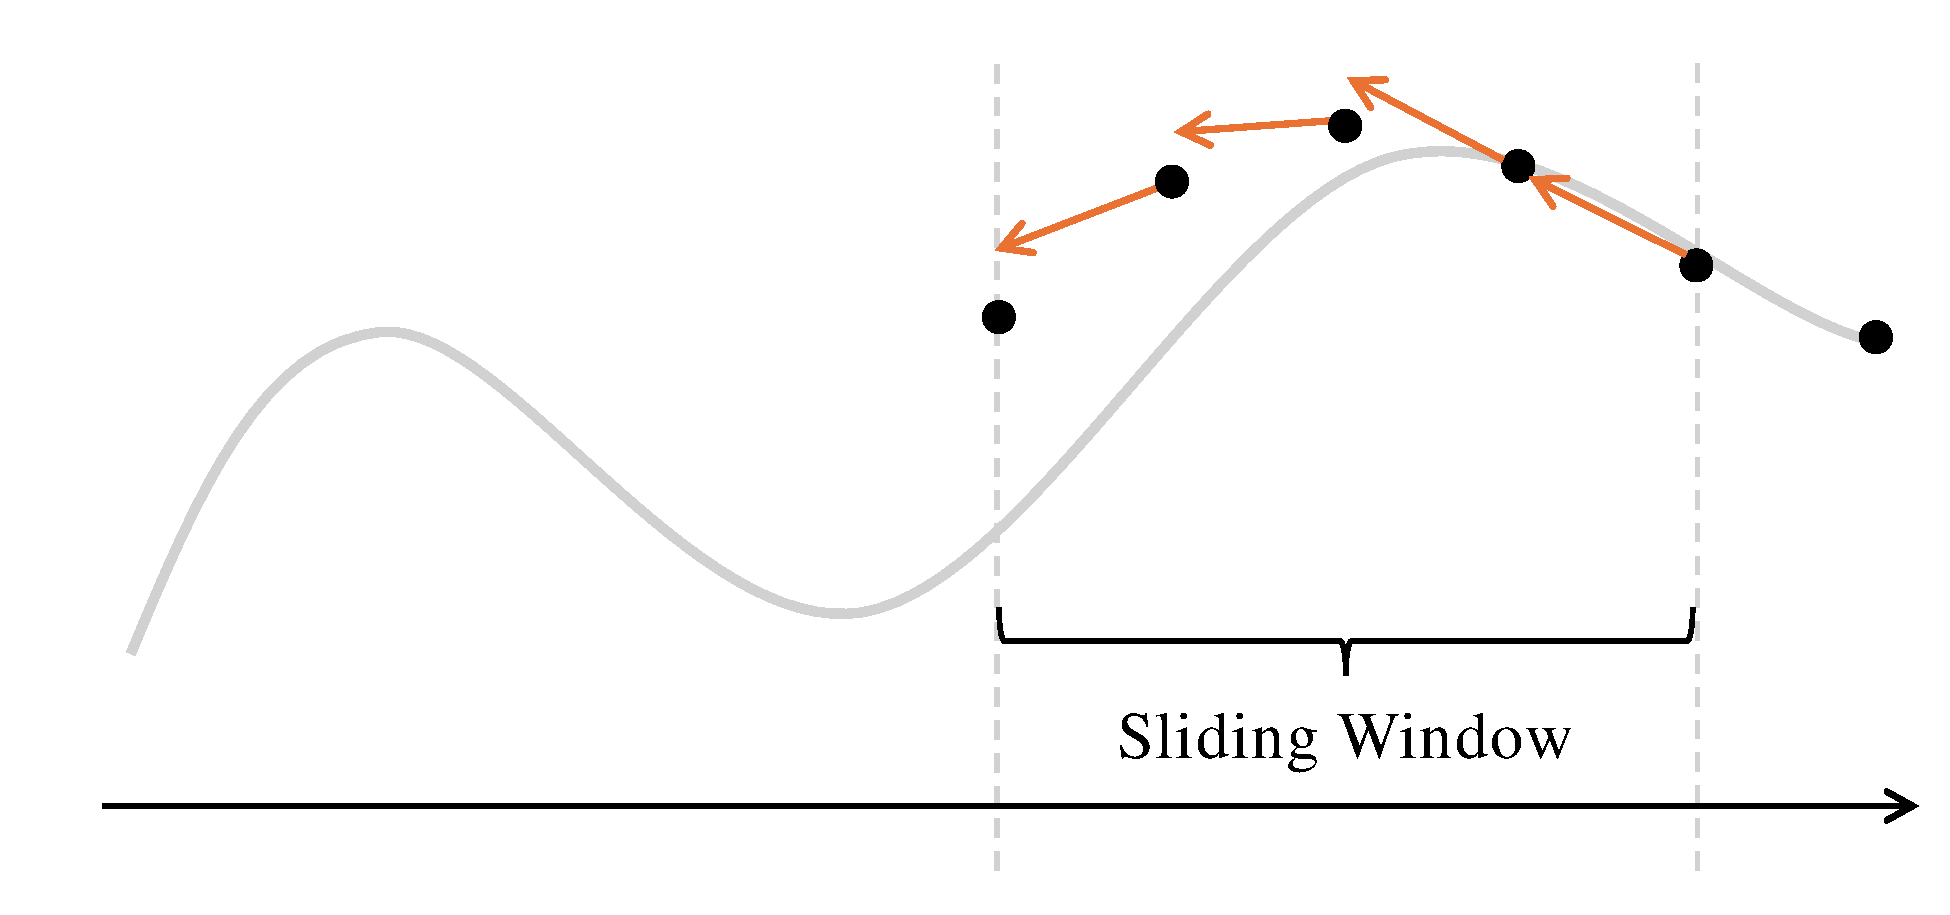
\includegraphics[width=\linewidth]{Images/PartC/paradigm-1.pdf}
        \caption{在大小为 $p=4$ 的批次窗口上并行计算 $\rvx^{(k)}_{\ell:\ell+p}$ 的漂移}
        \label{fig:picard_1}
    \end{minipage}%
    \hspace{0.03\textwidth} % To maintain the space between the images
    \begin{minipage}[t]{0.30\textwidth}
        \centering
        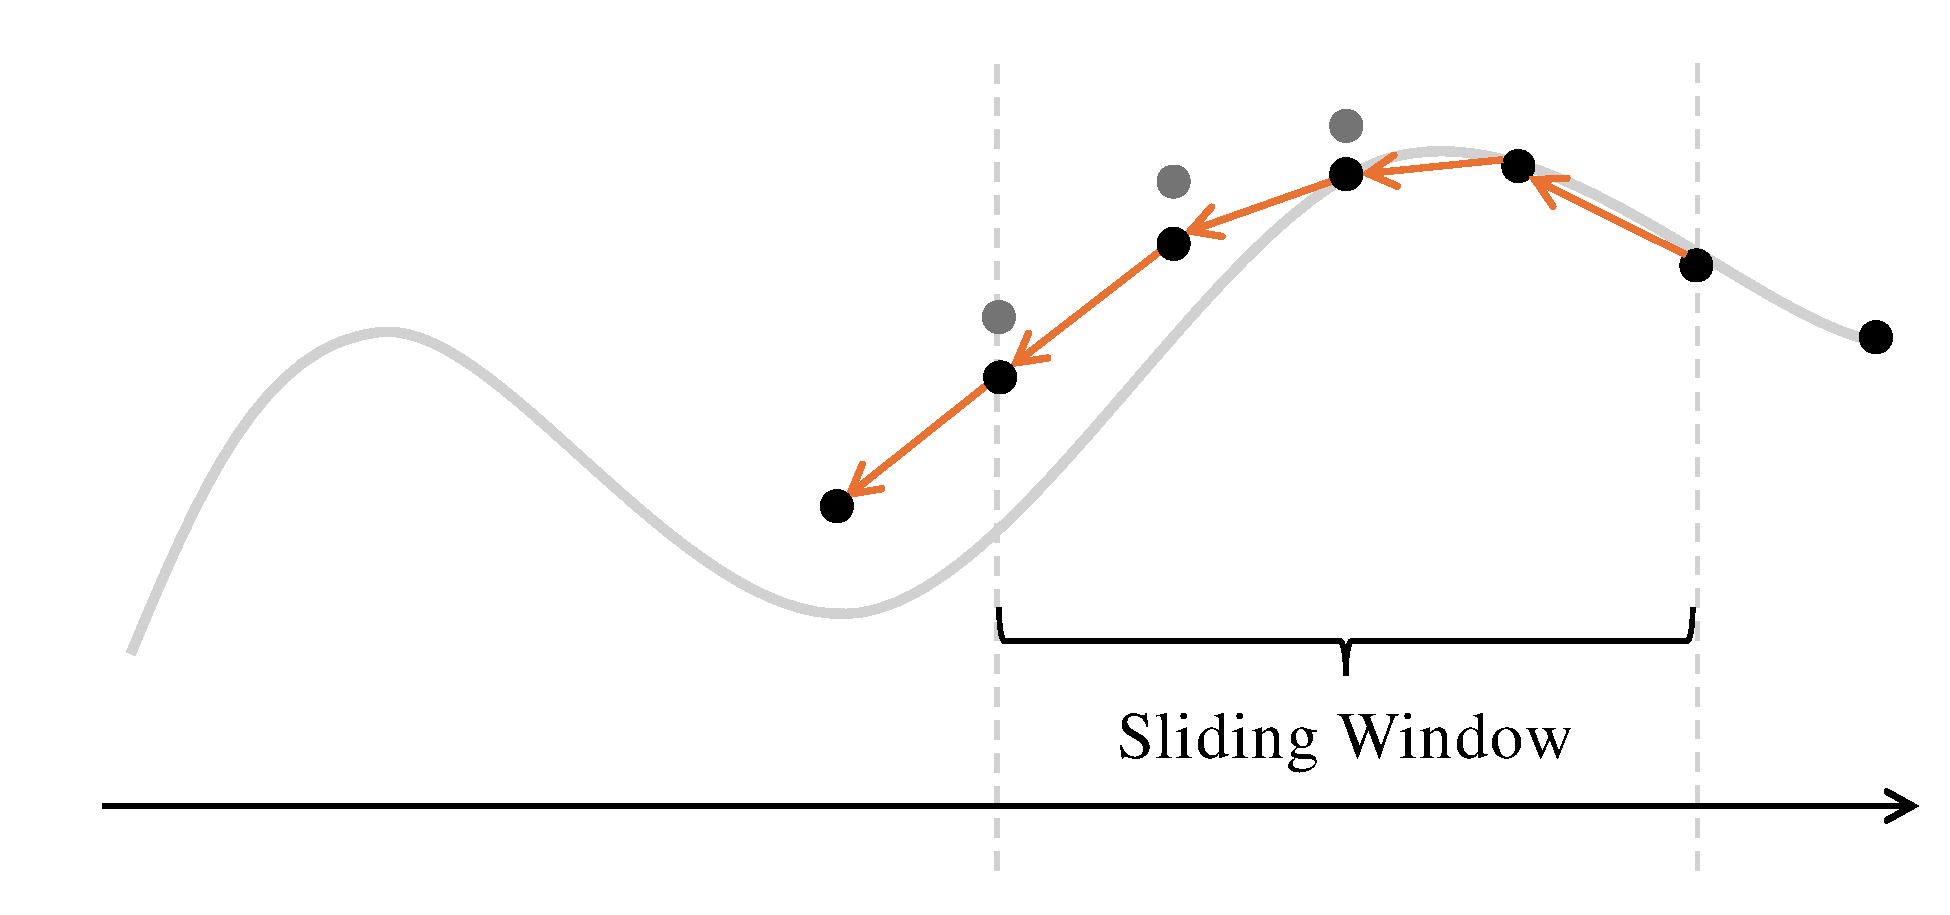
\includegraphics[width=\linewidth]{Images/PartC/paradigm-2.pdf}
        \caption{使用窗口内点的累积漂移更新值到 $\rvx^{(k+1)}_{\ell:\ell+p}$}
        \label{fig:picard_2}
    \end{minipage}%
    \hspace{0.03\textwidth} % To maintain the space between the images
    \begin{minipage}[t]{0.30\textwidth}
        \centering
        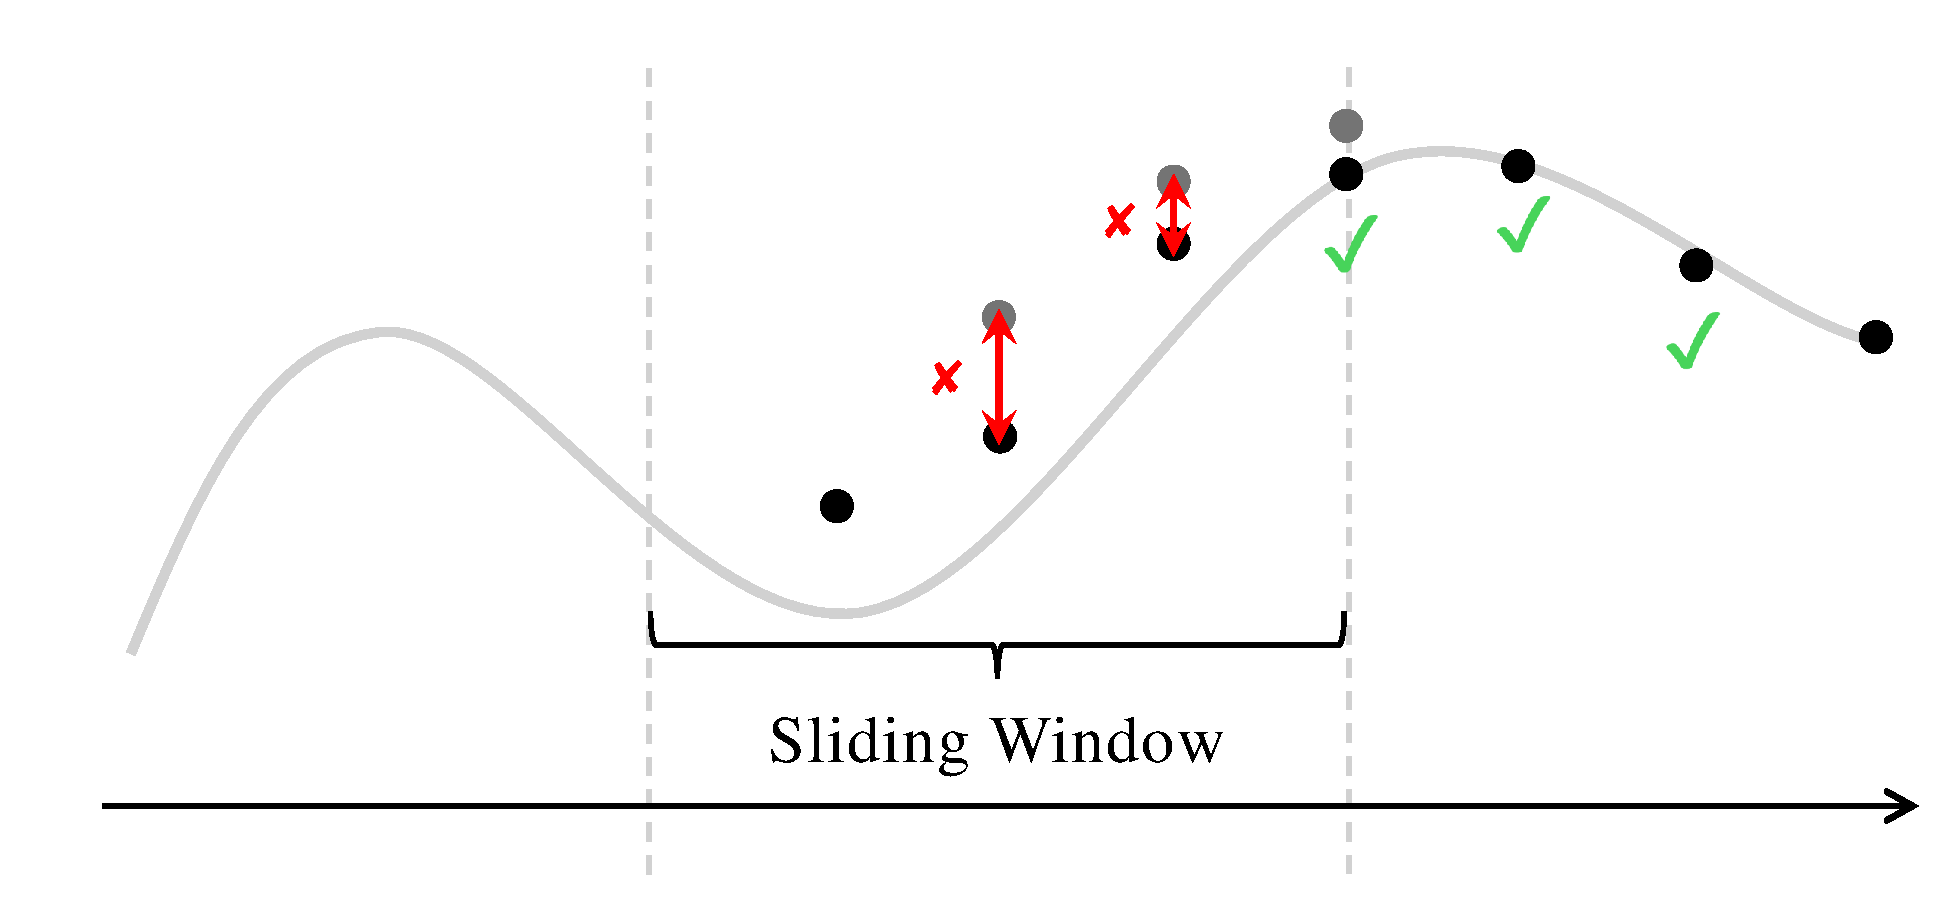
\includegraphics[width=\linewidth]{Images/PartC/paradigm-3.pdf}
        \caption{基于误差 $\lVert \rvx^{(k+1)}_i - \rvx^{(k)}_i \rVert^2$ 决定窗口向前滑动多远。}
        \label{fig:picard_3}
    \end{minipage}
    % \caption{During iteration $k$, ParaDiGMS processes a batch window of size $p$ spanning timesteps $[t,t+p)$ \textit{in parallel}. The new values at a point $\rvx^{(k+1)}_{t+j}$ are updated based on the value  $\rvx^{(k)}_j$ at the left end of the window, plus the cumulative drift  $1/T \sum_{i=t}^{t+j-1} \mathbf{F}_{\bm{\phi}^\times}(\rvx^{(k)}_{i}, i/T)$  of points within the window. We then slide the window forward until the error exceeds our tolerance, and repeat for the next iteration.}
    \figcredit{改编自 \citet{shih2023parallel}。}
    \label{fig:picard}
\end{figure}


离散 Picard 更新 \Cref{eq:discrete_picard_decreasing} 把每个 $\rvx^{(k+1)}_j$ 表示为左锚定的值 $\rvx^{(k)}_0$ 减去漂移的累加和。为限制内存并利用并行硬件，方便的做法是
把同一思想局部地应用于短的、滑动的索引块上。

固定窗口长度 $p$ 与左索引 $\ell$；则窗口覆盖
$j=\ell,\ldots,\ell+p$，其中 $t_\ell>t_{\ell+1}>\cdots>t_{\ell+p}$。在第
$k$ 次迭代中：

\subparagraph{第 1 步。窗口上的并行漂移求值。}
并行地、仅用上一次迭代，计算
\[
\rvv_{\bphi^\times} \big(\rvx^{(k)}_{\ell+i}, t_{\ell+i}\big),
\quad i=0,1,\ldots,p-1.
\]
它们是从左边缘
$t_\ell$ 跨越窗口推进所需的 $p$ 个局部增量。

\subparagraph{第 2 步。左锚定的累积更新。}
以 $j=\ell$ 锚定并跨子区间累积漂移，形成窗口化更新：
\begin{equation}\label{eq:window_update}
\rvx^{(k+1)}_{\ell+j+1}
 = 
\rvx^{(k)}_{\ell}
 - \Delta t \sum_{i=0}^{j}
\rvv_{\bphi^\times} \big(\rvx^{(k)}_{\ell+i}, t_{\ell+i}\big),
\quad j=0,1,\ldots,p-1.
\end{equation}
这正是 \Cref{eq:discrete_picard_decreasing} 限制在
窗口上的情形，减号反映了递减的时间方向。内层
求和是窗口化漂移上的前缀和（扫描），因此所有部分和
都可以在并行硬件上高效产生。

\subparagraph{第 3 步。进度控制与窗口推进。}
在当前窗口上形成左锚定的累积更新（第 2 步）之后，
我们现在决定该窗口向前滑动多远。我们用逐点 Picard 变化量
\[
\mathtt{error}_j
:=
\big\|\rvx^{(k+1)}_{\ell+j}-\rvx^{(k)}_{\ell+j}\big\|^2,
\quad j=1,\ldots,p-1,
\]
度量局部收敛性，
并将其与规定的容差 $\mathtt{tol}_{\ell+j}$ 比较。即 $\mathtt{error}_j$ 度量节点 $\ell+j$ 处的迭代在上一次 Picard
更新中变化了多少。若该值很小，则表明两次相继近似在该节点处的局部一致，从而该节点处的不动点
迭代局部收敛。若该值很大，则该节点尚未稳定，需要
更多 Picard 平滑。


\emph{步长}选为窗口中第一个未通过此检验的索引（若无失败则为完整窗口长度 $p$）：
\[
\mathtt{stride}
:=
\min\Big(\,\{\,j\ge 1:\ \mathtt{error}_j>\mathtt{tol}_{\ell+j}\,\}\ \cup\ \{p\}\Big).
\]
然后我们通过令 $\ell \leftarrow \ell+\mathtt{stride}$ 来滑动窗口。换言之：我们接受从左边缘起直至（但不包括）第一个未收敛节点的所有节点；若所有节点都已收敛，我们接受
整个窗口。然后我们按所接受的节点数滑动窗口，
$\ell \leftarrow \ell+\mathtt{stride}$，并继续。这最多前进
窗口长度 $p$，绝不跳过任何未达到其
容差的节点。若滑动会越过网格末端 $M$，我们把窗口截断为
$p \leftarrow \min\{p,\,M-\ell\}$ 并继续。



当窗口向前移动时，它会暴露出尚无
值的新时间节点。为在那里启动 Picard 迭代，我们简单地复制
窗口左边界处的值作为初始猜测。这种“常数外推”廉价且稳定，会被后续
更新修正。若需要，可用从过去点出发的线性
或多项式外推等更准确的猜测来替代它。

这就完成了 ParaDiGMS 的流程。我们在 \Cref{alg:paradigms} 中总结算法。


\begin{algorithm}[t]
  \caption{带滑动窗口的 ParaDiGMS}
  \label{alg:paradigms}
  \begin{algorithmic}[1]
    \Require 漂移 $\rvv_{\bphi^\times}(\rvx,t)$；$\{t_j\}_{j=0}^{M}$；窗口长度 $p$；$\{\mathtt{tol}_j\}_{j=1}^{M}$
    \Ensure 近似轨迹 $\{\rvx^{(k)}_j\}_{j=0}^{M}$，其中 $\rvx^{(k)}_M$ 在 $t=0$ 处
    \State $k \gets 0$, $\ell \gets 0$ 
    \State 采样 $\rvx^{(0)}_0 \sim p_{\mathrm{prior}}$；对 $j=1,\ldots,\min(p,M)$ 置 $\rvx^{(0)}_j \gets \rvx^{(0)}_0$  \Statex \Comment{常数外推}
    \While{$\ell < M$}
      \State $J \gets \min(p,  M-\ell)$   \Comment{当前窗口长度}
      \State \textbfs{第 1 步：并行} 
      \State 对 $i=0,\ldots,J-1$：$g_i \gets \rvv_{\bphi^\times} \big(\rvx^{(k)}_{\ell+i},\, t_{\ell+i}\big)$ 
      \Statex \Comment{来自上一次迭代的漂移（Picard 冻结）}
      \State 计算前缀和 $S_j \gets \sum_{i=0}^{j} g_i$，$j=0,\ldots,J-1$ 
      \Statex \Comment{对窗口化漂移做扫描}
      \State \textbfs{第 2 步：累积更新} 
      \State 对 $j=0,\ldots,J-1$：$\displaystyle \rvx^{(k+1)}_{\ell+j+1} \gets \rvx^{(k)}_{\ell} - \Delta t\, S_j$ 
      \Statex \Comment{左锚定更新；参见 \Cref{eq:window_update}}
      \State \textbfs{第 3 步：进度控制与窗口推进} 
      \State 对 $j=1,\ldots,J-1$：$\mathtt{error}_j \gets \big\|\rvx^{(k+1)}_{\ell+j}-\rvx^{(k)}_{\ell+j}\big\|^2$ \Statex \Comment{逐点 Picard 变化量}
      \State $\displaystyle \mathtt{stride} \gets \min \Big(\,\{\,j\in\{1,\ldots,J-1\}:~\mathtt{error}_j>\mathtt{tol}_{\ell+j}\,\}\ \cup\ \{J\}\Big)$
      \State \textbfs{初始化新节点} 
      \State 对 $r=1,\ldots,\mathtt{stride}$：$\rvx^{(k+1)}_{\ell+J+r} \gets \rvx^{(k+1)}_{\ell+J}$ 
      \Statex \Comment{对新暴露索引的常数外推}
      \State $\ell \gets \ell + \mathtt{stride}$;\quad $k \gets k+1$
    \EndWhile
    \State \Return $\{\rvx^{(k)}_j\}_{j=0}^{M}$
  \end{algorithmic}
\end{algorithm}




\subsection{与时间步进求解器的关系}

\paragraph{滑动窗口大小的选择。}

为把滑动窗口方案置于背景中，首先注意最小窗口大小时会发生什么。当 $p=1$ 时，窗口包含单步，故
\Cref{eq:window_update} 退化为 PF--ODE 的一阶时间步进更新。例如，若我们采用与 DDIM 相同的 ODE 写法（如数据 vs. 噪声预测）并选择与 DDIM 相同的离散时间步调度，则该方法退化为 DDIM。

增大 $p$ 扩展了并行性（每个窗口推进更多节点）而不
改变总步数 $M$。因此，样本质量继续
由基础离散化（网格/参数化的选择
和每步公式）连同每个窗口上的 Picard 收敛决定，
我们通过局部容差来监控。 

\paragraph{与高阶求解器（如 DPM）的兼容性。}
滑动窗口 Picard 结构控制的是增量\emph{如何}计算
（并行并由扫描累积），而不是\emph{哪个}局部公式定义
那些增量。因此，人们可以用任意
一致的高阶求积替换左端点规则而不改变并行
布局。例如，\Cref{eq:window_update} 的梯形变体为
\begin{align*}
    \begin{aligned}
        \rvx^{(k+1)}_{\ell+j+1}
=
\rvx^{(k)}_{\ell}
-\Delta t \Big[
\tfrac{1}{2}\rvv_{\bphi^\times} \big(\rvx^{(k)}_{\ell},t_{\ell}\big)
+\sum_{i=1}^{j-1}\rvv_{\bphi^\times} \big(\rvx^{(k)}_{\ell+i},t_{\ell+i}\big)
+\tfrac{1}{2}\rvv_{\bphi^\times} \big(\rvx^{(k)}_{\ell+j},t_{\ell+j}\big)
\Big],
    \end{aligned}
\end{align*}
其中所有漂移仍取自上一次 Picard 迭代，因此
逐节点求值保持独立，内层求和仍为前缀和。

类似地，DPM 求解器家族使用的多步或指数积分器更新
（例如 log--SNR 时间中的 DPM--Solver\texttt{++} $2$M）可以通过
用过去模型求值（$\rvx$-或 $\beps$-预测配以预计算
系数）的相应高阶线性组合替换每个窗口化增量来插入。
然后扫描像之前一样在窗口上累积那些加权增量。简言之：并行方案与近似积分的求解器（离散化）选择无关。精度来自基础求解器；窗口化前缀和只是让它变快。

\newpage
\section{结语}\label{sec:ch9_cr}

本章直面扩散模型最重要的实际局限之一：其缓慢的迭代采样过程。我们探索了一类强大的免训练解决方案，它们通过利用微分方程数值方法的丰富领域来加速生成。核心策略是更高效地求解 PF-ODE，该 ODE 定义了从噪声到数据的确定性生成轨迹：
\begin{enumerate}
    \item 我们从基础的 DDIM 开始，它可以被理解为一阶指数 Euler 方法。
    \item 然后转向像 DEIS 这样的高阶多步方法，它们通过使用过去求值的历史来提升精度。
    \item 最后，我们考察了高效的 DPM-Solver 家族，它通过引入关键的 log-SNR 时间重参数化实现了卓越的性能。
\end{enumerate}

通过这些高级求解器，高质量生成所需的函数评估次数（NFE）已从数百或数千次大幅减少到少至 10-20 次，使扩散模型显著更实用。

然而，这些免训练方法在根本仍然是迭代的。它们一步步地近似一条连续路径。这引出一个自然且雄心勃勃的问题：\emph{我们能否仅用一步或极少数离散步实现高质量生成？}

本书的最后部分 D 将通过基于训练的加速来探索这一问题。我们将研究两种主要策略：
\begin{enumerate}
    \item 首先，在 \Cref{ch:distillation} 中，我们将考察基于蒸馏的方法，其中一个快速的 \textit{学生} 生成器被训练以在远更少的步数内复现一个缓慢、预训练的 \textit{教师} 扩散模型的输出。
    \item 然后，在 \Cref{ch:fast-scratch} 中，我们将通过探索从头学习快速、少步生成器的方法把这一思想推得更远，例如一致性训练（Consistency Training），它定义了一种独立的训练原理而不依赖任何预训练模型。
\end{enumerate}

这种从改进求解器到直接学习解映射本身的转变，代表了高效生成式建模的前沿，旨在把扩散模型的质量与单步生成器的速度结合起来。


% \begin{itemize}
%     \item When $p=1$, ParaDiGMS reduces to the Euler method, equivalent to DDIM.
%     \item ParaDiGMS is compatible with any time-stepping ODE solver, including DDIM, DEIS, and the DPM-solvers family, among others.
%     \item ParaDiGMS does not degrade sample quality as it does not aim to reduce the number of sampling timesteps. 
% \end{itemize}


\clearpage
\newpage


\part{迈向学习快速的扩散生成器}
% \documentclass[../Main.tex]{subfiles}
% \externaldocument{0.0.overview}



% \begin{document}
\chapter{用于快速采样的基于蒸馏的方法}\label{ch:distillation}

本章介绍基于训练的方法，通过训练新的生成器使其仅需一步或几步即可产生样本，从而加速扩散模型的采样。其核心思想被称为\emph{蒸馏}（distillation），即让一个快速的学生模型（student model）向一个缓慢、预训练好的扩散模型（教师模型，teacher）采样器学习。虽然教师模型可能需要数百步，学生模型却能在仅需几步的情况下达到可比的质量\footnote{此处蒸馏指的是减少采样步数，而非缩小模型规模。}。与改进数值积分格式的求解器加速不同，蒸馏直接训练生成器走高效的捷径。我们重点介绍两种主要范式：\emph{分布级蒸馏}（distribution level distillation），它跳过对完整轨迹的模拟，转而使学生模型的输出分布与教师模型的分布对齐；以及\emph{流映射级蒸馏}（flow map level distillation），它训练学生模型以更快、更紧凑的方式复现教师模型的采样路径。

% This chapter introduces training-based methods for obtaining a one- or few-step denoiser (generator) for fast sampling by assuming an access to some well-trained pre-trained DM $\rvs_{\bm{\phi}^\times}(\rvx_s, s) \approx \nabla_{\rvx_s} \log p_s(\rvx_s)$. With the pre-trained DM, it can provides a proxy to $p_{\mathrm{data}}$ via sampling trajectory (i.e., SDE/ODE solving) as highlighted in \Cref{subsec:sde-sample}. the  The high-level idea of common approaches is either to distill the trajectory, or the learned distributions of a pre-trained diffusion model (teacher) into a fewer-steps generator from noise to a clean estimate.




% , which is supposed to be a proxy to $p_{\mathrm{data}}$ while sampling from its requires SDE/ODE solving as highlighted in \Cref{subsec:sde-sample}. Many approaches were proposed to extract either its sampling trajectory (we call it \emph{Trajectory Distillation}) into a few step generators or extract distribution modeled by the pre-trained DM (we refer to \emph{Distributional Distillation})
\clearpage
\newpage


\section{引言}\label{sec:distillation-prologue}
扩散模型的一个核心瓶颈是其缓慢的采样速度。

如 Tweedie 公式（\Cref{subsec:four-equiv-para}）所示，扩散模型可以解释为一个“$\rvx$-预测”模型 $\rvx_{\bm{\phi}^\times}(\rvx_t, t)$，它被训练为在噪声水平 $t$ 下从带噪输入 $\rvx_t$ 恢复期望的干净数据：
\[
    \rvx_{\bm{\phi}^\times}(\rvx_t, t) \approx \mathbb{E}[\rvx_0 |\rvx_t],
\]
其中期望是关于 $p(\rvx_0 |\rvx_t)$ 取的，表示与 $\rvx_t$ 对应的所有可能干净数据。
一个自然的想法是用 $\rvx_{\bm{\phi}^\times}(\rvx_t, t)$ 进行一步生成。但由于该去噪器对许多可能结果进行了平均，预测会变得过度平滑，仅用少量去噪步骤进行生成会导致模糊、低质量的样本。

另一方面，如 \Cref{subsec:sde-sample} 所讨论的，扩散采样沿 ODE 或 SDE 轨迹经历一长串迭代步骤。这产生了高保真度的样本，但所需的大量步数使得该过程本质上是缓慢的。降低 NFE（即采样步数乘以模型调用次数）可以加快生成，但不可避免地会降低保真度。
每个求解器步长都引入 $\mathcal{O}(h^{n})$ 阶的积分误差，
其中 $n$ 是求解器阶数，$h=\max_i |t_i - t_{i-1}|$ 是步长。
步数越少意味着时间增量 $h$ 越大，这又反过来增加了累积的采样误差，导致轨迹精度下降。
这在扩散采样的质量与效率之间造成了根本性的权衡。

为克服这一瓶颈，一条重要的研究路线是\emph{蒸馏}，它假设可以访问一个训练良好的扩散模型（\emph{教师模型}），并训练一个生成器（\emph{学生模型}）通过单次前向或几步计算来复现其行为。
这把教师模型的许多采样步骤压缩成一个快速过程，在保持高样本保真度的同时有效地绕过了缓慢的迭代求解器。




下面，我们介绍关于蒸馏的两种视角：\emph{分布级蒸馏}和\emph{流映射级蒸馏}\footnote{从时间顺序上看，以 \emph{Knowledge Distillation}（KD）~\citep{luhman2021knowledge} 和 \emph{Progressive Distillation}（PD）~\citep{ho2020denoising} 为代表的流映射级蒸馏更早于 2021 年提出，早于 2023 年前后兴起的分布级蒸馏方法家族。不过，为了叙述更顺畅并与下一章衔接，我们先介绍分布级蒸馏。}。




\subsection{分布级蒸馏}
基于分布的蒸馏的目标是训练一个单步生成器 $\rmG_{\bm{\theta}}(\rvz)$，它将噪声 $\rvz \sim p_{\mathrm{prior}}$ 映射到样本 $\hat\rvx = \rmG_{\bm{\theta}}(\rvz)$，从而诱导一个分布 $p_{\bm{\theta}}(\hat\rvx)$，用以逼近目标数据分布 $p_{\mathrm{data}}(\rvx)$。这通常通过最小化某个统计散度来实现
\[
\min_{\bm{\theta}}  \mathcal{D}\!\left(p_{\bm{\theta}}(\hat\rvx),  p_{\mathrm{data}}(\hat\rvx)\right),
\]
其中 $\mathcal{D}$ 表示某个合适的散度度量，例如 KL。

在实践中，基于分布的方法将生成器的分布与预训练扩散模型所产生的经验分布 $p_{\bm{\phi}^\times}(\rvx)$ 对齐：
\[
\min_{\bm{\theta}}  \mathcal{D}\!\left(p_{\bm{\theta}}(\hat\rvx),  p_{\bm{\phi}^\times}(\hat\rvx)\right),
\]
其中 $p_{\bm{\phi}^\times}$ 充当 $p_{\mathrm{data}}$ 的代理。这些方法并不显式地计算该散度，而是逼近其梯度，而该梯度可以直接从预训练教师模型计算得到。
这使得学生模型能够将其分布与教师模型对齐，而无需完整的散度求值。

这一表述通过分布对齐将扩散模型的多步生成过程蒸馏为单步模型。我们在 \Cref{sec:VSD} 中详细阐述该方法。




\subsection{流映射级蒸馏} 我们考虑 PF-ODE，它可以用任意预测模型表示（见 \Cref{eq:predictions-equivalence}）：
\begin{align}\label{eq:pf-ode-ct}
    \frac{\diff \rvx(\tau)}{\diff \tau} 
    = f(\tau) \rvx(\tau) - \tfrac{1}{2}g^2(\tau) \nabla_\rvx \log p_\tau(\rvx(\tau)) 
    =: \rvv^*(\rvx(\tau), \tau).
\end{align}

其解映射记为 $\bPsi_{s\to t}(\rvx_s)$，表示从时间 $s$ 的 $\rvx_s$ 出发反向演化到时间 $t \leq s$；即
\begin{align}\label{eq:int_target_gt}
\begin{aligned}
    \bPsi_{s\to t}(\rvx_s) 
    &\coloneqq \rvx_s + \int_s^t \rvv^*(\rvx(\tau), \tau) \diff \tau,
\end{aligned}
\end{align}
其中积分求解的是 PF-ODE。直观地说，$\bPsi_{s\to t}$ 将时间 $s$ 的噪声 $\rvx_s$ 输运到时间 $t$ 处噪声更少的状态（最终在 $t=0$ 时成为数据）。


从扩散模型采样对应于对 $\rvx_T \sim p_{\mathrm{prior}}$ 求值 $\bPsi_{T\to 0}(\rvx_T)$。通常，该积分由利用速度场 $\rvv$ 的迭代数值求解器逼近（见 \Cref{ch:solvers}），但需要许多步（例如 DPM-Solver 中至少 $10$ 步），使得采样比 GAN 等经典单步生成模型更慢。这引出一个自然的问题：
\begin{question}
    我们能否直接学习解映射 $\bPsi_{s\to t}(\rvx_s)$？
\end{question}
特别地，学习映射 $\bPsi_{T\to 0}(\rvx_T)$（其中 $\rvx_T \sim p_{\mathrm{prior}}$）即可实现单步生成。


\paragraph{轨迹蒸馏。}

轨迹蒸馏旨在训练一个神经生成器，在实例层面逼近解映射。由于 PF-ODE 积分很少有闭式形式，训练时必须对其进行数值逼近。为形式化，我们引入通用的求解器记号
\begin{align}\label{eq:solver}
    \mathtt{Solver}_{s\to t}(\rvx_s;\,\bm{\phi}^\times)
    \quad \text{or simply} \quad
    \mathtt{Solver}_{s\to t}(\rvx_s),
\end{align}
表示从 $s$ 到 $t$、以 $\rvx_s$ 为起点对经验 PF-ODE 进行数值积分，
使用教师参数 $\bm{\phi}^\times$（在上下文清楚时省略）。



\paragraph{一种早期方法：直接知识蒸馏。}
为了实现少步乃至单步生成，一种直接的方法是训练一个生成器 $\rmG_\btheta(\rvx_T, T,0)$，去模仿沿完整轨迹求值的数值求解器输出：
\[
\rmG_\btheta(\rvx_T, T,0)\approx \mathtt{Solver}_{T\to 0}(\rvx_T), 
\qquad \rvx_T \sim p_{\mathrm{prior}}.
\]
这一思想是早期轨迹蒸馏方法之一——\emph{知识蒸馏}（Knowledge Distillation）~\citep{luhman2021knowledge} 的基础，它使用回归损失
\[
\mathcal{L}_{\mathrm{KD}}(\btheta)
:= 
\E_{\rvx_T \sim p_{\mathrm{prior}}}
\left\|
\rmG_\btheta(\rvx_T, T,0)
-
\mathtt{Solver}_{T\to 0}(\rvx_T)
\right\|_2^2.
\]
虽然该方法能提供来自预训练教师模型的直接监督，
但它无法利用原始训练数据中可获得的强监督。
此外，若在训练循环中调用 ODE 积分，计算开销会非常昂贵，因为每次参数更新都需要求解 ODE 来构造目标。
最后，由于生成器只学到从 $T$ 到 $0$ 的全局映射，它可能会失去从中间状态操控生成过程的可控性。因此，\Cref{ch:guidance} 中介绍的大多数可控生成技术无法直接应用。




\paragraph{渐进式蒸馏的前言。}
\emph{渐进式蒸馏}（Progressive Distillation，PD）~\citep{salimans2021progressive} 使用来自 $\mathtt{Teacher}$ 片段的\emph{局部}监督来训练一个时间条件化的 $ \mathtt{Student} $。
设 $t_0=T>t_1>\cdots>t_N=0$ 为固定的时间网格。
$ \mathtt{Teacher} $ 为 $k=0,\ldots,N-1$ 提供时间步进映射 $\mathtt{Teacher}_{t_k\to t_{k+1}}$。


PD 并非只监督单跳 $T\to 0$，而是训练 $ \mathtt{Student}  $ 的两步跨越映射来匹配两个连续的 $ \mathtt{Teacher}$ 步：
\[
\mathtt{Student}_{t_k\to t_{k+2}}
\;\approx\;
\mathtt{Teacher}_{t_{k+1}\to t_{k+2}}
\circ
\mathtt{Teacher}_{t_{k}\to t_{k+1}},
\]
其中 $k = 0, 2, 4, \dots$。
匹配使用简单的回归损失（如均方误差）。


在局部配对片段上训练之后，$ \mathtt{Student} $ 不再沿原始网格的每个时间区间前进。
相反，它在每隔一个时间点上前进，
\[
t_0 \to t_2 \to t_4 \to \cdots \to t_N,
\]
这意味着每个 $ \mathtt{Student} $ 步实际上覆盖了两个连续的 $ \mathtt{Teacher}$ 步。
因此，$ \mathtt{Student} $ 仅用 $N/2$ 次转移即可完成相同的总时间跨度 $[0,T]$。

在此阶段之后，训练好的 $ \mathtt{Student} $ 取代 $ \mathtt{Teacher}$，作为新的参考模型。
然后整个流程在更稀疏的网格上重复，时间步长加倍
$(N \to N/2 \to N/4 \to \cdots)$，
逐步将轨迹蒸馏为越来越少的步数，直到达到所需的推理步数。
这种迭代式减半在保持全局时间跨度的同时，不断压缩生成过程的时间分辨率。






\paragraph{流映射学习的统一视角。}
包括 KD 和 PD 在内的多种方法都可以纳入统一的损失框架：
\begin{align}\label{eq:general-cm-loss}
  \mathcal{L}_{\mathrm{oracle}}(\btheta)
  := \E_{s,t} \E_{\rvx_s \sim p_s} 
  \left[  w(s,t)  d \big(\rmG_\btheta(\rvx_s, s,t),  \bPsi_{s\to t}(\rvx_s)\big)\right],
\end{align}
其中 $\bPsi_{s\to t}$ 是 oracle 流映射，$w(s,t) \geq 0$ 指定不同时间对 $(s,t)$ 的加权方式，
$d(\cdot,\cdot)$ 是差异度量，例如
$d(\rvx,\rvy)=\|\rvx-\rvy\|_2^2$ 或 $d(\rvx,\rvy)=\|\rvx-\rvy\|_1$，而 $p_s$ 表示时间 $s$ 处前向加噪的边缘分布。由于 $\bPsi_{s\to t}$ 没有闭式表达，
必须依赖近似，通常通过预训练扩散模型（教师模型）或其他可处理的代理。

KD 表现为
\Cref{eq:general-cm-loss} 的一个简单实例。选取退化的加权
$w(s,t)=\delta(s{-}T)\,\delta(t{-}0)$ 并使用先验分布
$p_T=p_{\mathrm{prior}}$\footnote{该假设在 $T$ 足够大或采用合适的噪声调度 $(\alpha_t,\sigma_t)$ 时成立。}，oracle 损失 $\mathcal{L}_{\mathrm{oracle}}(\btheta)$ 简化为：
\[
\E_{\rvx_T\sim p_T}
\big\|\rmG_\btheta(\rvx_T,T,0)-\bPsi_{T\to 0}(\rvx_T)\big\|_2^2
\approx \mathcal{L}_{\mathrm{KD}}(\btheta),
\quad
\]
其中 $\mathtt{Solver}_{T\to 0}\approx\bPsi_{T\to 0}$。\Cref{app-sec:flow-map} 给出了该表述的另一种视角。


PD 也符合这一模板，但它并非只用单个极端时间对 $(T,0)$ 进行监督，而是使用许多\emph{邻近}的时间对，并施加一个简单的\emph{局部一致性}规则：
一次短步接着另一次短步应当匹配直接的两步移动。我们在 \Cref{eq:pd-local} 中再回到这一点。

在实践中，主要挑战在于 oracle 流映射 $\bPsi_{s\to t}$ 通常没有闭式表达，使得直接监督不可行。已有多种方法被开发出来以高效地逼近这一
目标，但它们的成功往往取决于教师模型
的质量。我们将在 \Cref{ch:fast-scratch} 中再次回到 \Cref{eq:general-cm-loss}，提出一个用于从头训练方法的原理性框架，将教师模型从学习循环中去除。









\clearpage
\newpage



\section{\texorpdfstring{基于分布的蒸馏}{Distribution-Based Distillation}}\label{sec:VSD}


多项工作在不同名称下并行开展了基于分布的蒸馏研究，
包括 Distributional Matching Distillation（DMD）~\citep{yin2024one,yin2024improved}、
Variational Score Distillation（VSD）~\citep{pooledreamfusion,wang2023prolificdreamer,luo2023diff,lu2024simplifying}
和 Score Identity Distillation（SiD）~\citep{zhou2024score}。
尽管技术细节有所不同，它们共享同一原理：
训练一个生成器，使其前向加噪后的边缘分布与教师模型相匹配。
我们以 VSD 作为代表性表述重点介绍，因为其他方法遵循类似的原理。


\subsection{作为代表性方法的 VSD 表述}
\paragraph{前向过程。}
设 $\{p_t\}_{t \in [0,T]}$ 表示由下式诱导的前向扩散过程的边缘密度
\[
\rvx_t = \alpha_t \rvx_0 + \sigma_t \bm{\epsilon}, \quad \bm{\epsilon} \sim \mathcal{N}(\bm{0}, \rmI),
\]
其初始分布为 $p_0 = p_{\mathrm{data}}$。
相反地，设 $p_0^{\bm{\theta}}$ 为确定性单步生成器 $\rmG_{\bm{\theta}}(\rvz)$ 从隐变量 $\rvz \sim p_{\mathrm{prior}}(\rvz)$ 生成的合成样本所构成的分布。定义 $\{p_t^{\bm{\theta}}\}_{t \in [0,T]}$ 为对 $p_0^{\bm{\theta}}$ 施加相同前向扩散过程所得到的边缘密度，即
\begin{align}\label{eq:vsd-forward}
    \rvx_t^{\bm{\theta}} := \alpha_t \rmG_{\bm{\theta}}(\rvz) + \sigma_t \bm{\epsilon}, 
\end{align}
其中 $\rvz \sim p_{\mathrm{prior}}$，$ \bm{\epsilon} \sim \mathcal{N}(\bm{0}, \rmI)$。因此，$p_t$ 和 $p_t^{\bm{\theta}}$ 共享同一高斯扩散核
$p_t(\rvx_t| \rvx_0)$，但起始分布不同
（分别为 $p_{\mathrm{data}}$ 与单步合成样本的 $p_0^{\bm{\theta}}$）。

\paragraph{训练目标与梯度。}
文献中通常采用 KL 散度来匹配分布 $p_t$ 与 $p_t^{\bm{\theta}}$，一般通过最小化
\begin{align*}
    \mathcal{L}_{\text{VSD}}(\bm{\theta}) &:=\mathbb{E}_t \left[ \omega(t)  \mathcal{D}_{\text{KL}}(p_t^{\bm{\theta}} \, \| \, p_t) \right]
\\&= \mathbb{E}_{t, \rvz, \bm{\epsilon}} \left[ \omega(t) \left( \log p_t^{\bm{\theta}}(\rvx_t^{\bm{\theta}}) - \log p_t(\rvx_t^{\bm{\theta}}) \right) \right],
\end{align*}
其中 $\omega(t)$ 是时间相关的加权函数。我们将在 \Cref{subsec:vsd-discussion} 讨论 KL 散度为何在分布级蒸馏中
扮演特殊角色。



如 \citep{wang2023prolificdreamer} 所示，最优解在 $ p_0^{\bm{\theta}^*} = p_{\mathrm{data}} $ 时取得，这表明生成器的分布与数据分布匹配，因此该训练目标是学习数据分布的有效损失。

然而，基于密度的目标表述缺乏高效的训练机制。幸运的是，对 $\bm{\theta}$ 求梯度，我们得到 \Cref{eq:vsd-grad} 中的表达式，下面以命题形式总结。为记号简洁，我们将 \Cref{eq:vsd-forward} 中定义的 $\rvx_t^{\bm{\theta}}$ 记为 $\hat\rvx_t$。




\proppp{$\mathcal{L}_{\text{VSD}}$ 的 $\bm{\theta}$-梯度}{vsd-grad}{
我们有
\begin{align}\label{eq:vsd-grad}
\begin{aligned}
        &\nabla_{\bm{\theta}}\mathcal{L}_{\text{VSD}}(\bm{\theta}) \\= &\mathbb{E}_{t, \rvz, \bm{\epsilon}} \left[ \omega(t)\alpha_t  \left( 
\nabla_{\rvx} \log p_t^{\bm{\theta}}(\hat\rvx_t) - \nabla_{\rvx} \log p_t(\hat\rvx_t) 
\right) \cdot \partial_{\bm{\theta}} \rmG_{\bm{\theta}}(\rvz) \right].
\end{aligned}
\end{align}
}{
推导应用链式法则：
\begin{align*}
&\nabla_{\btheta} \E_t \left[ \mathcal{D}_{\mathrm{KL}}(p_t^{\btheta}\|p_t) \right]
\\&= \E_{t,\rvz,\beps}\!\left[\partial_\btheta
\big(\log p_t^{\btheta}(\hat\rvx_t)-\log p_t(\hat\rvx_t)\big) \right] \\
&= \E_{t,\rvz,\beps} \left[ 
 \underbrace{\partial_{\btheta}\log p_t^{\btheta}(\hat\rvx_t)}_{\text{first}}
+ (\nabla_{\rvx}\log p_t^{\btheta}(\hat\rvx_t))^\top \partial_{\btheta}\hat\rvx_t
- (\nabla_{\rvx}\log p_t(\hat\rvx_t))^\top \partial_{\btheta}\hat\rvx_t \right].
\end{align*}
第一项由分数函数恒等式而为零：
\[
\E_{\hat\rvx_t\sim p_t^{\btheta}}\!\left[\partial_{\btheta}\log p_t^{\btheta}(\hat\rvx_t)\right]
= \int \partial_{\btheta} p_t^{\btheta}(\rvx)  \diff\rvx
= \partial_{\btheta}  \int p_t^{\btheta}(\rvx)  \diff\rvx
= \partial_{\btheta}(1)=0.
\]
利用重参数化 $\hat\rvx_t=\alpha_t\rmG_{\btheta}(\rvz)+\sigma_t\beps$ 可得
$\partial_{\btheta}\hat\rvx_t=\alpha_t\partial_{\btheta}\rmG_{\btheta}(\rvz)$，因此
\[
\nabla_{\btheta}\mathcal{L}_{\text{VSD}}(\btheta)
= \E_{t,\rvz,\beps} \left[\omega(t) \alpha_t 
\big(\nabla_{\rvx}\log p_t^{\btheta}(\hat\rvx_t)-\nabla_{\rvx}\log p_t(\hat\rvx_t)\big)^\top
\partial_{\btheta}\rmG_{\btheta}(\rvz)\right].
\]
这就证明了 \Cref{eq:vsd-grad}。
细节见 \Cref{app-sec:flow-map}。
}


我们观察到，对 $\bm{\theta}$ 求梯度时，分数函数自然地出现。因此，我们需要逼近单步生成器的分数 $\nabla_{\rvx}\log p_t^{\bm{\theta}}(\hat\rvx_t)$，以及数据分布的 $\nabla_{\rvx}\log p_t(\hat\rvx_t)$，下文将详述。









\subsection{VSD 的训练流程}\label{subsec:vsd-training}
现有工作~\citep{yin2024one,yin2024improved,pooledreamfusion,wang2023prolificdreamer,luo2023diff,lu2024simplifying} 通常通过双层优化方法来解决：在 $\rmG_{\bm{\theta}}(\rvz)$ 产生的样本上训练一个新的扩散模型来逼近 $\nabla_{\rvx} \log p_t^{\bm{\theta}}(\hat\rvx_t)$，并采用预训练扩散模型来为合成样本 $\hat\rvx_t$ 上不可处理的 oracle 分数函数 $\nabla_{\rvx} \log p_t(\hat\rvx_t)$ 提供代理。更准确地说，训练在两个阶段之间交替进行：
\begin{itemize}
    \item \textbfs{分数估计阶段。} 固定 $\bm{\theta}$。令 $\hat{\rvx}_0=\rmG_{\bm{\theta}}(\rvz)$，
    $\hat{\rvx}_t=\alpha_t \hat{\rvx}_0+\sigma_t\beps$，其中 $\rvz\sim p_{\mathrm{prior}}$，$\beps\sim\mathcal{N}(\bm{0},\rmI)$。
    利用已知的高斯扩散核 $p_t(\rvx_t|\rvx_0)$ 通过 DSM 训练 $s_{\bm{\zeta}}$：
    \[
    \mathcal{L}_{\text{DSM}}(\bm{\zeta};\bm{\theta})
    =\E_{t,\rvz,\beps}\Big\|\,\rvs_{\bm{\zeta}}(\hat{\rvx}_t,t)
    - \nabla_{\rvx_t}\log p_t(\hat{\rvx}_t|\hat{\rvx}_0)\,\Big\|^2,
    \]
    在最优处（对固定的 $\bm{\theta}$）得到 $\rvs_{\bm{\zeta}}(\cdot,t)\approx \nabla_{\rvx}\log p_t^{\bm{\theta}}(\cdot)$。
    

  \item \textbfs{生成器更新阶段。} 冻结 $s_{\bm{\zeta}}$（stop-grad），使用 \Cref{eq:vsd-grad} 中的梯度更新 $\bm{\theta}$，将各分数项替换为各自的代理：
  \[
    \rvs_{\bm{\zeta}}(\hat\rvx_t,t)\approx \nabla_{\rvx}\log p_t^{\bm{\theta}}(\hat\rvx_t), \,\, \text{and} \,\, \rvs_{\bm{\phi}^\times}(\hat{\rvx}_t,t)\approx \nabla_{\rvx}\log p_t(\hat\rvx_t)\ \ \text{(teacher)}.
  \]
  \Cref{eq:vsd-grad} 则近似为：
  \[
    \nabla_{\bm{\theta}}\mathcal{L}_{\text{VSD}}(\bm{\theta})
    \approx \mathbb{E}_{t,\rvz,\bm{\epsilon}}\Big[\omega(t)\alpha_t
      \big(\rvs_{\bm{\zeta}}(\hat{\rvx}_t,t) - \rvs_{\bm{\phi}^\times}(\hat{\rvx}_t,t)\big)^{\top}
      \partial_{\bm{\theta}}\rmG_{\bm{\theta}}(\rvz)
    \Big].
  \]
\end{itemize}
这两个阶段反复迭代，直到对所有 $t$，在 $p_t^{\bm{\theta}}$ 的支撑集上
$\rvs_{\bm{\zeta}}(\cdot,t)\approx \rvs_{\bm{\phi}^\times}(\cdot,t)$，
于是 \Cref{eq:vsd-grad} 中的代入式梯度消失。在此收敛情形下，
对所有 $t>0$，有 $p_t^{\bm{\theta}}\approx p_t^{\bm{\phi}^\times}$（教师模型的边缘分布）。
由于前向加噪算子（高斯卷积）对任意固定的 $t>0$ 都是单射，
因此 $p_0^{\bm{\theta}}\approx p_0^{\bm{\phi}^\times}$（教师模型的 $t=0$ 分布）。
于是，学习到的单步生成器 $\rmG_{\bm{\theta}}$ 在 $t=0$ 处与教师模型的分布匹配；
当教师模型很好地逼近 $p_{\mathrm{data}}$ 时，进一步有 $p_0^{\bm{\theta}}\approx p_{\mathrm{data}}$。

\subsection{补充讨论：散度选择与 VSD 的应用}\label{subsec:vsd-discussion}


\paragraph{超越 KL：能否使用一般散度？}
原则上，可以用更一般的散度族替换 VSD 中的前向 KL 项
$\mathcal{D}_{\mathrm{KL}}(p_t^{\btheta}\|p_t)$，
例如 $f$-散度（见 \Cref{eq:f-div}）：
\[
\mathcal{D}_f(p_t^{\btheta}\|p_t)
= \int p_t(\rvx)  f\!\left(\frac{p_t^{\btheta}(\rvx)}{p_t(\rvx)}\right)\diff \rvx.
\]
然而，梯度
$\nabla_{\btheta}\mathcal{D}_f(p_t^{\btheta}\|p_t)$ 通过
$f'(r_t)$ 依赖于\emph{密度比}
\[
r_t(\rvx)=\frac{p_t^{\btheta}(\rvx)}{p_t(\rvx)},
\]
这对于\emph{隐式学生生成器}而言是不可处理的。
此处学生模型被称为\emph{隐式}的，因为它可以通过随机映射
$\hat\rvx_t=\alpha_t\rmG_\btheta(\rvz)+\sigma_t\beps$ 产生样本
$\hat\rvx_t$，但不为其诱导密度
$p_t^{\btheta}(\rvx)$ 提供闭式表达或似然。
因此，计算 $\mathcal{D}_f$ 的泛函导数
需要逐点访问 $r_t(\rvx)$ 或其对数梯度，而这在此设定下均无法求值。
一种常见的变通方法是引入辅助的评判器或判别器，通过
$f$-散度的变分形式来逼近密度比，如 $f$-GAN~\citep{nowozin2016f}，尽管这会引入
额外的网络和嵌套的极小极大优化。

相比之下，对于前向 KL，路径梯度简洁地简化为分数差形式（\Cref{eq:vsd-grad}）：
\[
\nabla_{\btheta}\mathcal{D}_{\mathrm{KL}}(p_t^{\btheta}\|p_t)
= \E\!\left[
  \big(\nabla_{\rvx}\log p_t^{\btheta}(\hat\rvx_t)
  - \nabla_{\rvx}\log p_t(\hat\rvx_t)\big)^\top
  \partial_{\btheta}\hat\rvx_t
\right].
\]
这种结构使得仅基于分数的可处理更新成为可能。教师模型的
预训练扩散模型已经提供 $\nabla_{\rvx}\log p_t(\cdot)$，
因此我们可以直接复用它，而无需学习辅助的密度比
估计器。这一表述产生了一个非对抗的训练目标，且保持完全
可微与计算高效。

\paragraph{仅用二维预训练扩散模型进行三维生成的 VSD。}
VSD~\citep{wang2023prolificdreamer} 及其更早的特例 SDS~\citep{pooledreamfusion}（其中生成器是以 $\btheta$ 参数化的 Dirac）最初是为 3D 场景引入的，此时 3D 与 2D 数据之间没有配对监督（即没有真值 3D 标签）。
设 $\btheta\in\R^d$ 表示 3D 场景的参数，$\rmR(\btheta)$ 为生成图像 $\hat{\rvx}_0:=\rmR(\btheta)$ 的可微渲染器。
前向加噪过程定义为
\[
\hat{\rvx}_t=\alpha_t\,\rmR(\btheta)+\sigma_t\beps,\quad \beps\sim\mathcal N(\bm 0,\rmI).
\]
预训练的 2D（图像）扩散教师模型提供分数
\[
\rvs_{\bphi^\times}(\hat{\rvx}_t,t|\rvc)\approx\nabla_{\hat{\rvx}_t}\log p_t(\hat{\rvx}_t|\rvc),
\]
可选地以文本 $\rvc$ 为条件。
目标是在每个 $t$ 处将噪声渲染结果的分布与教师模型的边缘分布对齐。
一个最小化的表述是渲染分布下的分数对齐（VSD）目标：
\[
\mathcal{L}^{\text{3D}}_{\text{VSD}}(\btheta)
:=\E_{t,\beps}\!\left[\omega(t)\,\big\|
\rvs_{\bm{\zeta}}(\hat{\rvx}_t,t)-\rvs_{\bphi^\times}(\hat{\rvx}_t,t|\rvc)
\big\|_2^2\right],
\quad \hat{\rvx}_t=\alpha_t\rmR(\btheta)+\sigma_t\beps,
\]
它通过渲染器将图像空间的分数引导传递到 3D 参数。
在更新 $\btheta$ 时将两个分数都视为关于 $\hat{\rvx}_t$ 的停止梯度，得到
\[
\nabla_{\btheta}\mathcal{L}^{\text{3D}}_{\text{VSD}}(\btheta)
=\E_{t,\beps}\!\left[\omega(t)\,\alpha_t\,
\big(\rvs_{\bm{\zeta}}-\rvs_{\bphi^\times}\big)^\top
\frac{\partial \rmR}{\partial\btheta}(\btheta)\right].
\]
当学生分数 $\rvs_{\bm{\zeta}}$ 被抑制（Dirac 生成器）时，该表述退化为 SDS~\citep{pooledreamfusion}。
在实践中，优化完全按 \Cref{subsec:vsd-training} 中所述交替进行：先在噪声渲染结果上更新学生分数，然后在两个分数上施加停止梯度来更新 $\btheta$。
为简洁起见，此处省略进一步的数学细节。




\clearpage
\newpage

\section{\texorpdfstring{渐进式蒸馏}{Progressive Distillation}}\label{sec:PD}


渐进式蒸馏（Progressive Distillation，PD）~\citep{salimans2021progressive} 由两个过程组成，二者共同使扩散模型更高效地学习 PF-ODE 轨迹。
其核心思想是逐步减少高质量采样所需的积分步数，同时保持对教师轨迹的保真度。
\begin{itemize}
    \item \textbfs{蒸馏操作：} 基于预训练教师模型（最初是扩散模型），将一个确定性采样器（如 DDIM）蒸馏成一个学生模型，使其仅用一半的采样步数即可复现相同的轨迹。
    \item \textbfs{渐进操作：} 迭代地重复此蒸馏过程，每次将步数减半，直到学生模型能在少量固定预算内（通常 $1$–$4$ 步）生成高质量样本。
\end{itemize}

\begin{figure}[th!]
    \centering
    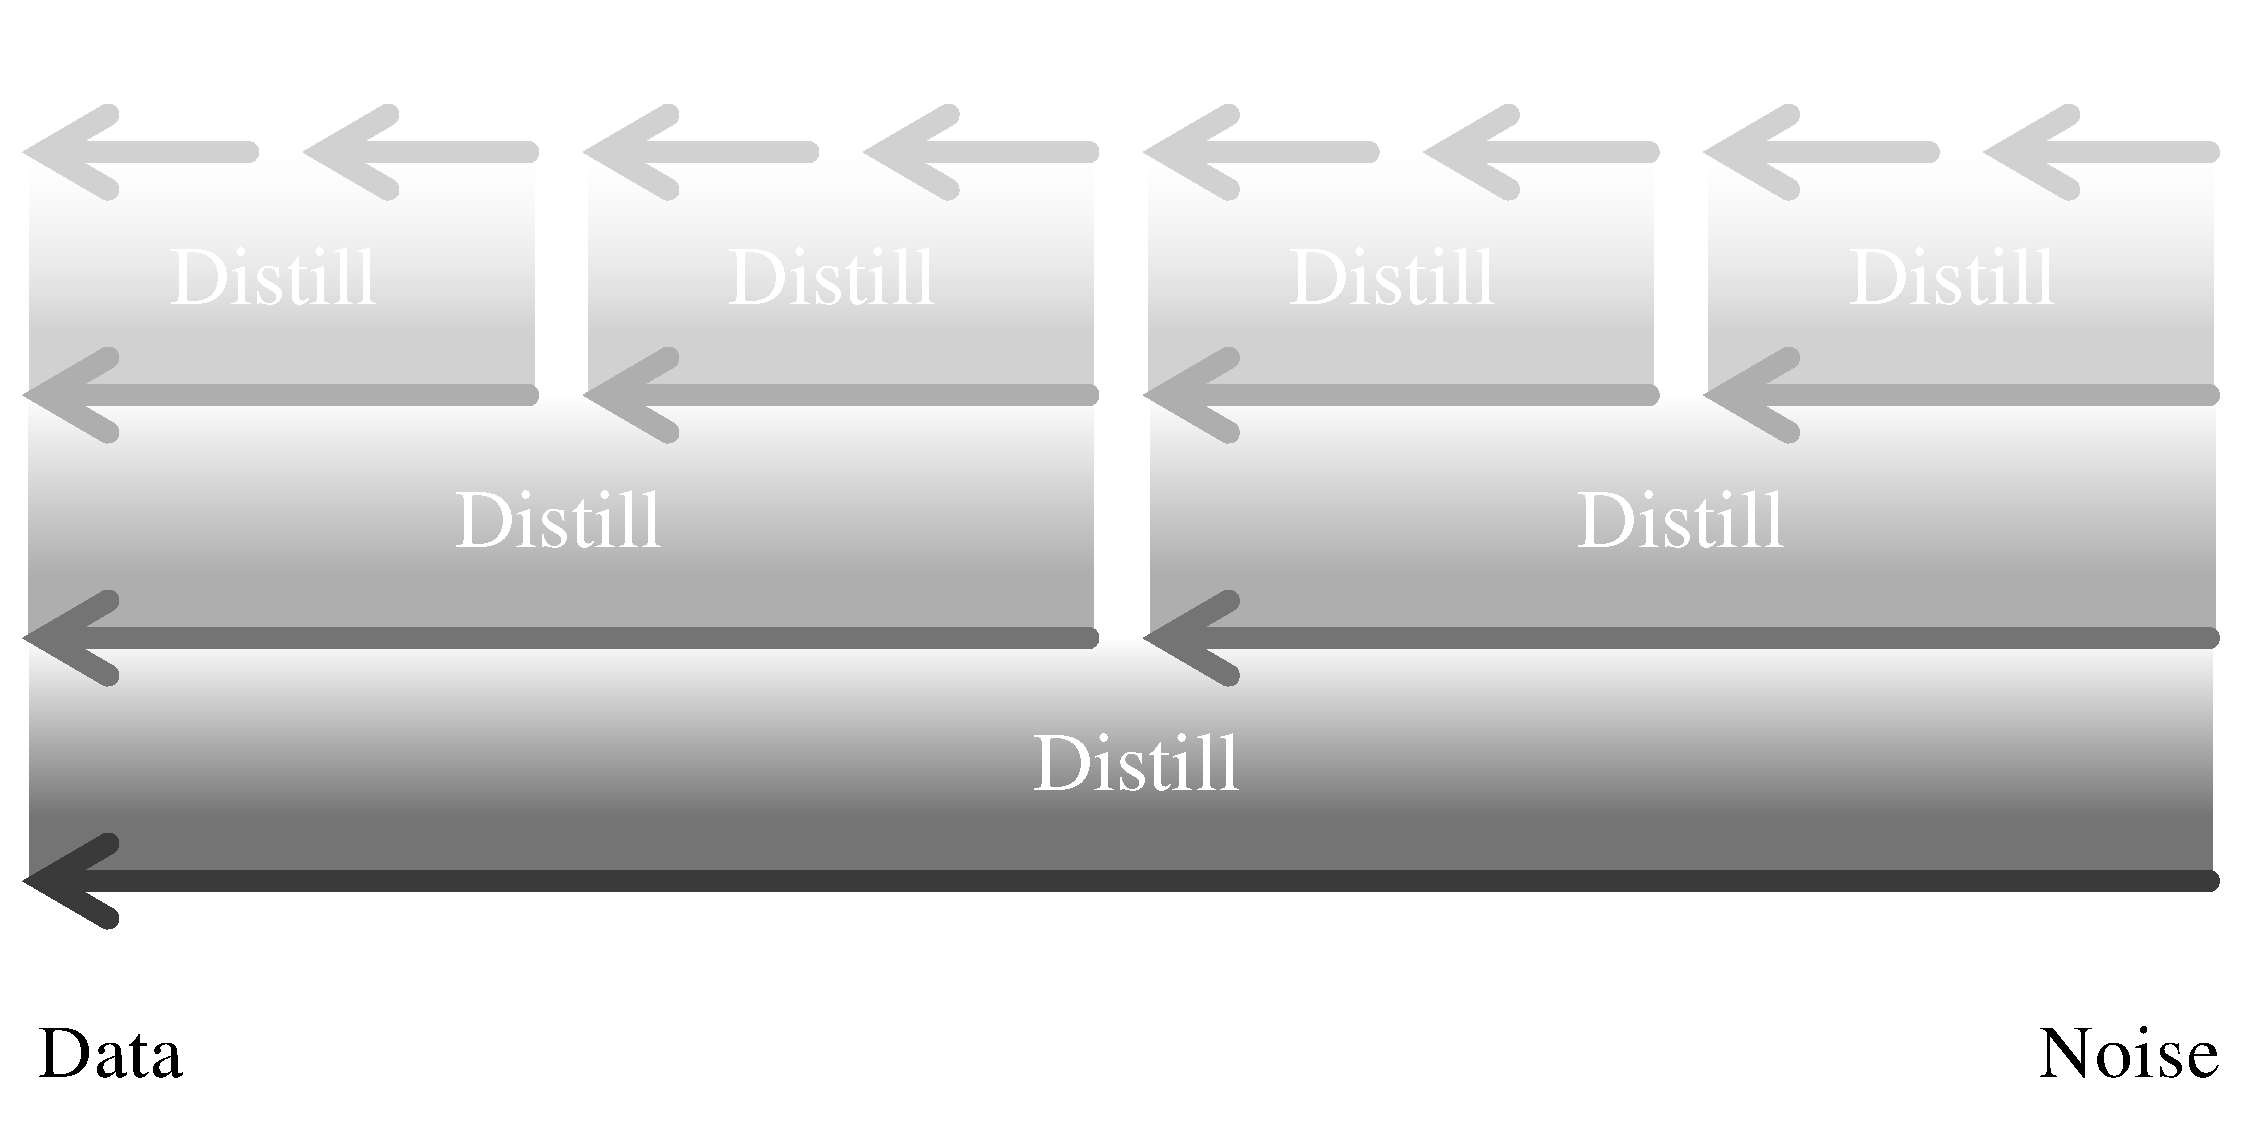
\includegraphics[width=0.93\linewidth]{Images/PartD/PD.pdf} 
    \caption{\textbfs{渐进式蒸馏（PD）示意图。}
在每一轮中，训练学生模型使得单步即可复现两个相邻教师步的效果。
该过程将 $N$ 个教师步蒸馏为 $N/2$ 个学生步，重复该过程可逐步将轨迹长度减半，直到达到所需的步数。
箭头表示多步教师转移如何被压缩为更少的学生步，从数据指向噪声。
\figcredit{由作者绘制。}
}
    \label{fig:pd-illustration}
\end{figure}



我们首先在 \Cref{subsec:pd-distillation} 中介绍 PD 的蒸馏操作，然后在 \Cref{subsec:pd-training} 中总结整个训练流程。\Cref{subsec:pd-guidance} 给出 CFG 引导的扩展。


\subsection{PD 中的蒸馏操作}\label{subsec:pd-distillation}

本节中，我们将 $\rvx$-预测参数化下的 DDIM 固定为时间步进规则，并仍将当前教师 $\rvx$-去噪器代入 DDIM 所得的确定性映射记为 $\mathtt{Solver}_{s \to t}$。


在第一轮 PD（教师 = 预训练扩散模型）中，这与通过 DDIM 积分扩散 PF-ODE 一致；在后续轮次（教师 = 上一轮学生）中，$\mathtt{Solver}_{s \to t}$ 仅仅是当前教师所诱导的 DDIM 转移，而非原始的扩散 PF-ODE。


蒸馏步骤如下：从带噪输入 $\rvx_s$（干净数据 $\rvx_s = \alpha_s \rvx_0 + \sigma_s \bm{\epsilon}$ 的扰动版本）出发，训练学生模型预测一个目标 ${\color{orange}\tilde\rvx}$，使得单步学生步 $s\!\to\! t$ 复现教师模型的两个连续步 $s\!\to\! u\!\to\! t$。
设 $\rvx_{\bm{\phi}^\times}(\rvx,\tau)$ 为本轮教师的 $\rvx$-预测去噪器。
将教师诱导的 DDIM 转移应用两次，得到
\[
\tilde\rvx_u := \mathtt{Solver}_{s\to u}\!\left(\rvx_s;\,\rvx_{\bm{\phi}^\times}\right),
\qquad
\tilde\rvx_t := \mathtt{Solver}_{u\to t}\!\left(\tilde\rvx_u;\,\rvx_{\bm{\phi}^\times}\right).
\]
这里我们使用 \Cref{eq:solver} 的记号，表示将 $\rvx_{\bm{\phi}^\times}$ 代入 DDIM 所诱导的、从 $s$ 到 $t$（以 $\rvx_s$ 为起点）的确定性转移映射。

\begin{question}
时间 $s$ 处的伪干净目标 ${\color{orange}\tilde\rvx}$ 是什么，使得求解器直接从 $s \to t$ 步进时产生与 $s \to u \to t$ 相同的输出 $\tilde\rvx_t$？具体而言，求满足下式的 ${\color{orange}\tilde\rvx}$：
\[
\tilde\rvx_t = \mathtt{Solver}_{s\to t}\left(\rvx_s; {\color{orange}\tilde\rvx}\right).
\]
\end{question}




一旦得到 ${\color{orange}\tilde\rvx}$ 的闭式表达，我们就训练一个学生模型 $\rvf_{\bm{\theta}}(\rvx_s, s)$（此处也是 $\rvx$-预测模型）来逼近“两步合一”目标 ${\color{orange}\tilde\rvx}$，最小化
\begin{align}\label{eq:pd-optimization}
\min_{\bm{\theta}} \E_s
\mathbb{E}_{\rvx_s\sim p_s}\!\left[w(\lambda_s)\,\big\|\rvf_{\bm{\theta}}(\rvx_s, s) - {\color{orange}\tilde\rvx}\big\|_2^2\right].
\end{align}


下面我们证明，DDIM 规则可通过初等代数给出 ${\color{orange}\tilde\rvx}$ 的闭式表达（注意该结果对离散时间和连续时间均成立）：
\lemp{DDIM 的“两步合一”目标 ${\color{orange}\tilde\rvx}$}{pd-ddim}{从初始条件 $\rvx_s$ 出发，若求解器取为 DDIM，则“两步合一”目标 ${\color{orange}\tilde\rvx}$ 可计算为
\begin{align*}
    {\color{orange}\tilde\rvx} 
    &=\frac{\sigma_s}{\alpha_t\sigma_s - \alpha_s\sigma_t} \tilde\rvx_t - \frac{\sigma_t}{\alpha_t\sigma_s - \alpha_s\sigma_t} \rvx_s.
\end{align*}
其中 $\tilde\rvx_t$ 由对 DDIM（\Cref{eq:ddim-update-all}）应用两次得到，路径为 $s \to u \to t$：
\begin{align*}
    s \to u: & \quad    && \tilde\rvx_u = \frac{\sigma_u}{\sigma_s}\rvx_s + \alpha_s \left(\frac{\alpha_u}{\alpha_s} - \frac{\sigma_u}{\sigma_s} \right)\rvx_{\bm{\phi}^\times}(\rvx_s, s)  \\
    u \to t: & \quad    && \tilde\rvx_t = \frac{\sigma_t}{\sigma_u}\tilde\rvx_u + \alpha_u \left(\frac{\alpha_t}{\alpha_u} - \frac{\sigma_t}{\sigma_u} \right)\rvx_{\bm{\phi}^\times}(\tilde\rvx_u, u).
\end{align*}
}{$\tilde\rvx_t$ 必须与从 $s$ 到 $t$ 的一步 DDIM $\tilde\rvx_t'$ 相匹配，其表达为：
\[
s \to t: \quad \tilde\rvx_t' = \frac{\sigma_t}{\sigma_s}\rvx_s + \alpha_s \left(\frac{\alpha_t}{\alpha_s} - \frac{\sigma_t}{\sigma_s} \right) {\color{orange}\tilde\rvx}.
\]
令 $\tilde\rvx_t'$ 与 $\tilde\rvx_t$ 相等，可解出 ${\color{orange}\tilde\rvx}$ 关于 $\tilde\rvx_t$、$s$、$t$ 的表达式：
\begin{align}
    &\tilde\rvx_t = \tilde\rvx_t' \nonumber \\
    \Longleftrightarrow\,\, & \tilde\rvx_t = \frac{\sigma_t}{\sigma_s}\rvx_s + \alpha_s \left(\frac{\alpha_t}{\alpha_s} - \frac{\sigma_t}{\sigma_s} \right) {\color{orange}\tilde\rvx} \nonumber \\
    \Longleftrightarrow\,\, & {\color{orange}\tilde\rvx} =  \frac{\tilde\rvx_t - \frac{\sigma_t}{\sigma_s}\rvx_s}{\alpha_s \left(\frac{\alpha_t}{\alpha_s} - \frac{\sigma_t}{\sigma_s} \right)} \label{eq:x-pd-paper} \\
    \Longleftrightarrow\,\, & {\color{orange}\tilde\rvx} = \frac{\sigma_s}{\alpha_t\sigma_s - \alpha_s\sigma_t} \tilde\rvx_t - \frac{\sigma_t}{\alpha_t\sigma_s - \alpha_s\sigma_t} \rvx_s. \nonumber
\end{align}
}
利用该公式，PD 在时间 $s$ 处计算伪干净目标，使其单步 DDIM 步进 $s\!\to\!t$ 恰好落到两步输出 $\tilde\rvx_t$。


\paragraph{实用的离散时间网格与损失。}
实践中，我们固定一个递减网格 $t_0=T>t_1>\cdots>t_N=0$，并为简洁记 $s:=t_k$，$u:=t_{k+1}$，$t:=t_{k+2}$。
教师模型提供单步映射 $\mathtt{Teacher}_{t_k\to t_{k+1}}$，学生模型学习一个两步跨越映射以匹配教师复合：
\[
\mathtt{Student}_{t_k\to t_{k+2}}
 \approx 
\mathtt{Teacher}_{t_{k+1}\to t_{k+2}}
\circ
\mathtt{Teacher}_{t_{k}\to t_{k+1}}.
\]

我们采样三元组 $(s,u,t)=(t_k,t_{k+1},t_{k+2})$，其中 $k\in\{0,\ldots,N-2\}$。
目标 \Cref{eq:pd-optimization} 变为
\[
\min_{\bm{\theta}} 
\mathbb{E}_{\,k \sim \mathcal{U}[\![0,N{-}2]\!]}\,
\mathbb{E}_{\,\rvx_{t_k}\sim p_{t_k}}\!
\Big[
  w(\lambda_{t_k})\,
  \big\|
  \rvf_{\bm{\theta}}(\rvx_{t_k},t_k) - {\color{orange}\tilde\rvx}^{(k)}
  \big\|_2^2
\Big],
\]
其中教师两步目标 ${\color{orange}\tilde\rvx}^{(k)}$ 通过引理~\ref{pd-ddim} 计算。若网格均匀，可写 $t_k = T(1 - k/N)$，从而
\[
s = T\Big(1 - \frac{k}{N}\Big),\quad
u = T\Big(1 - \frac{k+1}{N}\Big),\quad
t = T\Big(1 - \frac{k+2}{N}\Big),
\]
对应于步长 $\Delta s =  T/N$ 的均匀间隔时间步。


\subsection{PD 的完整训练流程及其采样}\label{subsec:pd-training}
通过 \Cref{eq:pd-optimization} 在局部配对片段上训练后，$\mathtt{Student}$ 不再沿原始网格的每个区间前进。相反，每个学习到的步覆盖两个连续的 $\mathtt{Teacher}$ 步，因此 $\mathtt{Student}$ 在每隔一个时间点上前进，
\[
t_0 \to t_2 \to t_4 \to \cdots \to t_N,
\]
从而仅用 $N/2$ 次转移即可遍历相同的跨度 $[0,T]$。此阶段之后，训练好的 $\mathtt{Student}$ 取代 $\mathtt{Teacher}$ 作为新的去噪器模型。然后该流程在更稀疏的网格（时间步长加倍）上重复，得到递进
\[
N \;\to\; N/2 \;\to\; N/4 \;\to\; \cdots,
\]
直到达到所需的推理步数。每次迭代中，新的 $\mathtt{Student}$ 由更新后的 $\mathtt{Teacher}$ 初始化。这种迭代式减半在保持全局时间跨度的同时，逐步压缩生成过程的时间分辨率。

\paragraph{采样。}
在推理时，使用当前 $\mathtt{Student}$ 作为去噪器的（DDIM）求解器，采样器在训练所诱导的稀疏网格上前进。第一轮后它做“跳 2”跳跃（$t_0 \to t_2 \to \cdots \to t_N$），下一轮后做“跳 4”（$t_0 \to t_4 \to \cdots \to t_N$），以此类推，每次迭代都将采样步数减半，同时保持相同的起止时间。

\subsection{补充讨论：局部半群匹配与广义求解器的可能性}


\paragraph{作为局部半群匹配的渐进式蒸馏。}
在统一目标 \Cref{eq:general-cm-loss} 中，不可处理的 oracle
目标 $\bPsi_{s\to 0}$ 被一个教师诱导的代理所替代，该代理使用
ODE 流的\emph{半群性质}（详见后文 \Cref{eq:semi-group}）：从 $s$ 演化到 $t$ 应当
等价于先从 $s$ 到任意中间点 $u$，再从 $u$ 到 $t$，
\[
\bPsi_{s\to t} = \bPsi_{u\to t}\circ\bPsi_{s\to u}.
\]
PD 通过训练学生单步映射匹配教师两个相邻单步片段的复合来局部地施加这一点：
\begin{align}\label{eq:pd-local}
  \E_{s}\E_{\rvx_s\sim p_s}
  \big\|
    \underbrace{\rmG_{\btheta}(\rvx_s, s, s-2\Delta s)}_{\text{student one-step}}
    -
    \underbrace{\mathtt{Solver}_{s-\Delta s\to s-2\Delta s}\big(\mathtt{Solver}_{s\to s-\Delta s}(\rvx_s)\big)}_{\text{teacher two-step composition}}
  \big\|_2^2.
\end{align}
最小化 \Cref{eq:pd-local} 在一个短递减网格上实例化半群恒等式（取 $s>u>t$，$u=s-\Delta s$，$t=s-2\Delta s$）：
\begin{align*}
  \bPsi_{s\to s-2\Delta s}
  &= \bPsi_{s-\Delta s\to s-2\Delta s}\circ\bPsi_{s\to s-\Delta s}
  \\&\approx
  \mathtt{Solver}_{s-\Delta s\to s-2\Delta s}\circ \mathtt{Solver}_{s\to s-\Delta s},
\end{align*}
因此训练只需要短的教师片段，而无需从时间 $s$ 一直
展开到 $0$。

为与 \Cref{eq:general-cm-loss} 中的少步去噪器视角联系起来，将
学生模型的少步映射定义为已学跳跃的复合：
\[
\underbrace{\rmG_{\btheta}(\rvx_s, s, 0)}_{\text{few-step denoiser}}
=
\big(\rmG_{\btheta}(\,\cdot\,, 2\Delta s, 0)\circ\cdots\circ \rmG_{\btheta}(\,\cdot\,, s, s-2\Delta s)\big)(\rvx_s).
\]
从概念上讲，\Cref{eq:pd-local} 为全局回归
\[
\E_{s,\rvx_s}\Big\|\rmG_{\btheta}(\rvx_s,s,0)\;-\;(\mathtt{Solver})^{\circ}_{s\to 0}(\rvx_s)\Big\|_2^2,
\]
提供了一个高效的\emph{局部代理}，
其中 $(\mathtt{Solver})^{\circ}_{s\to 0}$ 表示教师在步长为 $\Delta s$ 的网格上从 $s$ 到 $0$ 的完整
复合，作为 $\bPsi_{s\to 0}$ 的代理。

\paragraph{能否使用其他求解器？}
在上面对 PD 的介绍中，我们以 $\rvx$-预测参数化下的 DDIM 为具体的 PF-ODE 采样器进行了重点讨论。
带网格减半的局部半群匹配在确定性状态到状态映射的层面上是求解器无关的，并在参数化（$\rvx$、$\beps$、$\rvv$、score）之间进行标准转换后，可扩展到 \Cref{ch:solvers} 中的时间步进方法。
然而，此处的闭式伪目标依赖于\emph{单步、显式}更新，其单步映射对回归目标是\emph{仿射}的（如 DDIM 以及应用于 PF-ODE 的指数 Euler 或显式 RK 等显式单步格式）。
对于\emph{多步}或\emph{隐式}求解器（需要步历史或内层求解），应改为直接匹配相应的转移映射（参见 \Cref{eq:pd-local}）并提供必要的历史或热启动；一般而言不存在可比的闭式反演。

若采样器是随机的，则对每个样本固定噪声序列以获得确定性转移
$\mathtt{Teacher}^{(\omega)}_{s\to t}$（其中 $\omega$ 为固定的噪声种子）。
在这种情况下，PD 回归于一个固定的转移映射；闭式伪目标通常要求单步显式仿射更新；否则使用 \Cref{eq:pd-local} 中的直接匹配。









% In this section, we focus on DDIM in the $\rvx$-prediction parameterization as a concrete time–stepping rule.
% Here, $\mathtt{Solver}_{s \to t}$ denotes the current teacher’s deterministic transition map from $s$ to $t$, obtained by plugging the teacher denoiser into the same fixed update rule (DDIM).

% In the first PD round (teacher = pre–trained diffusion model), this coincides with integrating the diffusion PF–ODE via DDIM.
% In later rounds (teacher = previous student), $\mathtt{Solver}_{s \to t}$ remains the DDIM update induced by the current teacher denoiser; we do not identify it with the original diffusion PF–ODE.

% The distillation step is as follows: starting from a noisy input $\rvx_s$ (a perturbed version of clean data, $\rvx_s = \alpha_s \rvx_0 + \sigma_s \bm{\epsilon}$), the student is trained to predict a target ${\color{orange}\tilde\rvx}$ such that a single student step matches two teacher steps. More precisely, consider timesteps $s \to u \to t$, starting from $\rvx_s$.
% Let $\rvx_{\bm{\phi}^\times}(\rvx,\tau)$ denote the teacher’s $\rvx$-prediction denoiser in this round.
% Applying the teacher–induced DDIM transition twice gives
% \[
% \tilde\rvx_u := \mathtt{Solver}_{s\to u}\!\left(\rvx_s;\,\rvx_{\bm{\phi}^\times}\right),
% \qquad
% \tilde\rvx_t := \mathtt{Solver}_{u\to t}\!\left(\tilde\rvx_u;\,\rvx_{\bm{\phi}^\times}\right).
% \]
% Here, we use the notation of \Cref{eq:solver} to denote the deterministic transition map from $s$ to $t$ (starting at $\rvx_s$) induced by plugging $\rvx_{\bm{\phi}^\times}$ into DDIM.

% \begin{question}
% What is the pseudo-clean ${\color{orange}\tilde\rvx}$ at time $s$ such that the solver produces the same output $\tilde\rvx_t$ when stepping directly $s \to t$ as it does via $s \to u \to t$? Specifically, determine ${\color{orange}\tilde\rvx}$ satisfying:
% \[
% \tilde\rvx_t = \mathtt{Solver}_{s\to t}\left(\rvx_s; {\color{orange}\tilde\rvx}\right).
% \]
% \end{question}

% Once a closed-form expression for ${\color{orange}\tilde\rvx}$ is obtained, we train a student model $\rvf_{\bm{\theta}}(\rvx_s, s)$ (also an $\rvx$-prediction model here) to approximate the ``two-steps-in-one'' target ${\color{orange}\tilde\rvx}$ by minimizing
% \begin{align}\label{eq:pd-optimization}
% \min_{\bm{\theta}}\;
% \mathbb{E}_{\rvx_s\sim p_s}\!\left[w(\lambda_s)\,\big\|\rvf_{\bm{\theta}}(\rvx_s, s) - {\color{orange}\tilde\rvx}\big\|_2^2\right].
% \end{align}

% In the following, we show that the DDIM rule yields ${\color{orange}\tilde\rvx}$ in closed form via elementary algebra:
% \lemp{Two-Steps-in-One Target ${\color{orange}\tilde\rvx}$ of DDIM}{pd-ddim}{Starting from an initial condition $\rvx_s$, if the solver is taken as DDIM, then the ``two-step-in-one'' target ${\color{orange}\tilde\rvx}$ can be computed as
% \begin{align*}
%     {\color{orange}\tilde\rvx} 
%     % &=      \frac{\tilde\rvx_t - \frac{\sigma_t}{\sigma_s}\rvx_s  }{\alpha_s \left(\frac{\alpha_t}{\alpha_s} - \frac{\sigma_t}{\sigma_s} \right)} \\
%     &=\frac{\sigma_s}{\alpha_t\sigma_s - \alpha_s\sigma_t} \tilde\rvx_t - \frac{\sigma_t}{\alpha_t\sigma_s - \alpha_s\sigma_t} \rvx_s.
% \end{align*}
% Here, $\tilde\rvx_t$ is obtained by applying DDIM (in \Cref{eq:ddim-update-all}) twice, from $s \to u \to t$:
% \begin{align*}
%     s \to u: & \quad    && \tilde\rvx_u = \frac{\sigma_u}{\sigma_s}\rvx_s + \alpha_s \left(\frac{\alpha_u}{\alpha_s} - \frac{\sigma_u}{\sigma_s} \right)\rvx_{\bm{\phi}^\times}(\rvx_s, s)  \\
%     u \to t: & \quad    && \tilde\rvx_t = \frac{\sigma_t}{\sigma_u}\tilde\rvx_u + \alpha_u \left(\frac{\alpha_t}{\alpha_u} - \frac{\sigma_t}{\sigma_u} \right)\rvx_{\bm{\phi}^\times}(\tilde\rvx_u, u).
% \end{align*}
% }{$\tilde\rvx_t$ must be matched with the one-step DDIM from $s$ to $t$, $\tilde\rvx_t'$, expressed as:
% \[
% s \to t: \quad \tilde\rvx_t' = \frac{\sigma_t}{\sigma_s}\rvx_s + \alpha_s \left(\frac{\alpha_t}{\alpha_s} - \frac{\sigma_t}{\sigma_s} \right) {\color{orange}\tilde\rvx}.
% \]
% By equating $\tilde\rvx_t'$ and $\tilde\rvx_t$, we can solve for ${\color{orange}\tilde\rvx}$ in terms of $\tilde\rvx_t$, $s$, and $t$:
% \begin{align}
%     &\tilde\rvx_t = \tilde\rvx_t' \nonumber \\
%     \Longleftrightarrow\,\, & \tilde\rvx_t = \frac{\sigma_t}{\sigma_s}\rvx_s + \alpha_s \left(\frac{\alpha_t}{\alpha_s} - \frac{\sigma_t}{\sigma_s} \right) {\color{orange}\tilde\rvx} \nonumber \\
%     \Longleftrightarrow\,\, & {\color{orange}\tilde\rvx} =  \frac{\tilde\rvx_t - \frac{\sigma_t}{\sigma_s}\rvx_s}{\alpha_s \left(\frac{\alpha_t}{\alpha_s} - \frac{\sigma_t}{\sigma_s} \right)} \label{eq:x-pd-paper} \\
%     \Longleftrightarrow\,\, & {\color{orange}\tilde\rvx} = \frac{\sigma_s}{\alpha_t\sigma_s - \alpha_s\sigma_t} \tilde\rvx_t - \frac{\sigma_t}{\alpha_t\sigma_s - \alpha_s\sigma_t} \rvx_s. \nonumber
% \end{align}
% }
% With this formula, PD inverts a single DDIM update to compute the target value that the student must predict so that one student step arrives at ${\color{orange}\tilde\rvx}$.

% In practice, the discrete timestep $i$ is drawn uniformly as $i \sim \mathcal{U}[\![1,N]\!]$, and rescaled as
% \[
% s = \tfrac{i}{N}, \quad u = s - \tfrac{1}{2N}, \quad t = s - \tfrac{1}{N}.
% \]
% Thus, after the first distillation iteration, the teacher’s $N$-step sampler is compressed into a student model with $N/2$ steps.



% \subsection{Entire Training Pipeline of PD}\label{subsec:pd-training}
% After distilling the $2N$ steps of the teacher model into $N$ steps in the student model $\rmG_{\bm{\theta}}$ using \Cref{eq:pd-optimization}, the resulting $N$-step student model can be utilized as the new teacher. The same distillation procedure is then repeated to further distill the new teacher model into an $N/2$-step student model. At each iteration, the new student model is initialized with the parameters of the updated teacher model. This distillation process is progressively applied over multiple iterations.

% \paragraph{Sampling.}
% With the new student model serving as a denoiser in the empirical PF-ODE, the number of required sampling steps is halved at each iteration by utilizing the (DDIM) solver.


% \paragraph{Progressive Distillation as Local Semigroup Matching.}
% Within the unified objective \Cref{eq:general-cm-loss}, the intractable oracle
% target $\bPsi_{s\to 0}$ is replaced by a teacher–induced surrogate that uses the
% \emph{semigroup property} of the ODE flow (see more details later in \Cref{eq:semi-group}): evolving from $s$ to $t$ should be
% equivalent to going from $s$ to any intermediate $u$ and then from $u$ to $t$,
% \[
% \bPsi_{s\to t} \;=\; \bPsi_{u\to t}\circ\bPsi_{s\to u}.
% \]
% PD enforces this locally by training the student’s one–step map to match the
% teacher’s composition of two adjacent one–step fragments:
% \begin{align}\label{eq:pd-local}
%   \E_{s}\E_{\rvx_s\sim p_s}
%   \big\|
%     \underbrace{\rmG_{\btheta}(\rvx_s, s, s-2\Delta s)}_{\text{student one step}}
%     -
%     \underbrace{\mathtt{Solver}_{s-\Delta s\to s-2\Delta s}\big(\mathtt{Solver}_{s\to s-\Delta s}(\rvx_s)\big)}_{\text{teacher two-step composition}}
%   \big\|_2^2.
% \end{align}
% Minimizing \Cref{eq:pd-local} instantiates the semigroup identity on a short
% decreasing grid (take $s>u>t$ with $u=s-\Delta s$ and $t=s-2\Delta s$):
% \begin{align*}
%   \bPsi_{s\to s-2\Delta s}
%   &= \bPsi_{s-\Delta s\to s-2\Delta s}\circ\bPsi_{s\to s-\Delta s}
%   \\&\approx
%   \mathtt{Solver}_{s-\Delta s\to s-2\Delta s}\circ \mathtt{Solver}_{s\to s-\Delta s},
% \end{align*}
% so training only requires short teacher fragments, rather than a full rollout
% from time $s$ all the way to $0$.

% To connect back to the few–step denoiser view in \Cref{eq:general-cm-loss}, define
% the student’s few–step map as a composition of learned jumps:
% \[
% \underbrace{\rmG_{\btheta}(\rvx_s, s, 0)}_{\text{few-step denoiser}}
% =
% \big(\rmG_{\btheta}(\,\cdot\,, 2\Delta s, 0)\circ\cdots\circ \rmG_{\btheta}(\,\cdot\,, s, s-2\Delta s)\big)(\rvx_s).
% \]
% Conceptually, \Cref{eq:pd-local} provides an efficient \emph{local surrogate} for the
% global regression
% \[
% \E_{s,\rvx_s}\Big\|\rmG_{\btheta}(\rvx_s,s,0)\;-\;(\mathtt{Solver})^{\circ}_{s\to 0}(\rvx_s)\Big\|_2^2,
% \]
% where $(\mathtt{Solver})^{\circ}_{s\to 0}$ denotes the teacher’s full
% composition from $s$ to $0$ on a grid with step size $\Delta s$, serving as a
% proxy for $\bPsi_{s\to 0}$.

% In practice, PD proceeds by grid halving: start from an $N$–step teacher
% ($\Delta s=T/N$), learn $\rmG_{\btheta}(\,\cdot\,,\cdot,\,\cdot-2\Delta s)$ via
% \Cref{eq:pd-local} to obtain an $N$–step student, set this student as the new
% teacher, and iterate $N\to N/2\to N/4\to \cdots$ until reaching the
% target step count.



\subsection{带引导的 PD}\label{subsec:pd-guidance}
\citet{meng2023distillation} 提出了一种两阶段流程，用于蒸馏
无分类器引导（CFG）扩散模型：(1) 将引导\emph{蒸馏}
到一个以引导权重为输入的单网络中，(2) 应用
\emph{渐进式蒸馏（PD）}以减少采样步数。他们在像素空间和隐空间（如 Stable Diffusion）中均
验证了该方法。

\paragraph{第一阶段蒸馏：蒸馏引导。}
设 $\rvx_{\bm{\phi}^\times}(\rvx_s, s, \rvc)$ 为（预训练）条件
扩散模型在“$\rvx$-预测”参数化下（即干净估计）于时间 $s$、条件 $\rvc$ 处的输出；条件也可以
为空，$\rvc=\emptyset$（无条件分支）。\Cref{eq:cfg-model-nn} 中 $\omega$ 加权的 CFG
组合可写为
\begin{equation}\label{eq:cfg-model-clean}
   \rvx_{\bm{\phi}^\times}^{\,\omega}(\rvx_s, s, \rvc)
   := (1+\omega)\,\rvx_{\bm{\phi}^\times}(\rvx_s, s, \rvc)
      - \omega\,\rvx_{\bm{\phi}^\times}(\rvx_s, s, \emptyset),
\end{equation}
其中 $\omega \sim p_\omega(\omega)$，$p_\omega$ 为某个 CFG 加权分布，通常 $p_\omega(\omega)=\mathcal{U}[\omega_{\min},\omega_{\max}]$。

第一阶段引入一个新模型 $\rvx_{\bm{\theta}_1}(\rvx_s, s, \rvc, \omega)$，
它直接以 $\omega$ 为输入，通过监督
回归学习复现 CFG 输出 $\rvx_{\bm{\phi}^\times}^{\,\omega}(\rvx_s, s, \rvc)$：
\[
\min_{\bm{\theta}_1}\;
\mathbb{E}_{\omega\sim p_\omega, s, \rvx\sim p_{\mathrm{data}}, \rvx_s \sim p(\rvx_s\mid \rvx)}
\lambda(s)
\big\|\rvx_{\bm{\theta}_1}(\rvx_s, s, \rvc, \omega)-\rvx_{\bm{\phi}^\times}^{\omega}(\rvx_s, s, \rvc)\big\|_2^2.
\]
此处 $\lambda(s)$ 是标准的依赖调度的加权；每次迭代采样 $\omega$
教会单个网络在任意引导强度下模拟 CFG。

\paragraph{第二阶段蒸馏：PD。}
第一阶段模型 $\rvx_{\bm{\theta}_1}(\rvx_s, s, \rvc, \omega)$ 作为
PD 中的教师，按照 \Cref{subsec:pd-training} 被逐步蒸馏成一个采样步数更少的学生
$\rvx_{\bm{\theta}_2}(\rvx_s, s, \rvc, \omega)$。每次迭代步数
减半（例如 $N \to N/2 \to N/4 \to \cdots$）。

\newpage
\section{结语}\label{sec:ch10_cr}

本章介绍了我们的第一种主要的基于训练的加速范式。在通过数值求解器穷尽了无训练改进之后，我们将焦点转向一种新策略：训练一个快速的\textit{学生}生成器，使其学会复现一个缓慢、预训练的\textit{教师}扩散模型的行为。

我们探讨了两类主要的蒸馏思想。首先，在以 Variational Score Distillation（VSD）等为代表的分布级蒸馏中，通过在不同噪声水平上对齐各自的分数函数，训练学生模型的输出分布去匹配教师模型的分布，从而提供一个稳定、非对抗的目标。其次，在流映射蒸馏中，我们看到像渐进式蒸馏（PD）这样的方法训练学生模型直接逼近教师模型的解轨迹。PD 的迭代式方法——每一轮将采样步数减半——被证明是将一个漫长的迭代过程压缩为少数几步的强大而实用的方法。

这些蒸馏技术成功地弥合了迭代扩散模型的高样本质量与单步生成器推理速度之间的鸿沟，为高效、高保真合成提供了一条引人注目的路径。

然而，依赖预训练教师模型引入了两阶段流程：先训练一个缓慢但强大的教师，再将其蒸馏成一个快速的学生。这引出了生成式建模研究前沿的一个根本问题：我们能否完全绕过教师模型？

是否可能设计一种独立的训练原则，直接从数据学习这些快速的少步生成器？本书的最后一章将回答这个问题。
\begin{enumerate}
    \item 我们将探索诸如一致性模型（Consistency Models）等开创性方法，它们学习从 ODE 轨迹上任意一点到其终点之间的映射。
    \item 我们将深入探讨一致性模型的广义概念，它们学习在单步内将 ODE 轨迹上任意一点映射到另一点。
\end{enumerate}

这种从改进求解器或蒸馏解到直接学习解映射本身的转变，代表了向一类既原理化又在设计上高度高效的新型生成模型迈出的重要一步。

\clearpage
\newpage

\chapter{从零开始学习快速生成器}\label{ch:fast-scratch}

\epigraph{
    \textit{真理总是存在于简单之中，而非事物的繁多与混乱之中。
}}{Isaac Newton}


在\Cref{ch:distillation}中，我们看到扩散模型中缓慢的迭代采样器可以通过蒸馏压缩为少步生成器。从工程角度来看，两阶段流水线是实用的，因为它将复杂的生成式训练任务划分为清晰、独立的目标。第一阶段学习数据分布，第二阶段加速采样或提升质量。这种分离允许每个阶段独立优化，使整个系统更易管理、更稳定、更可靠。

然而，本章的重点转向驱动深度生成式建模进展的一个核心问题：
\begin{question}
    我们能否设计一种独立的生成原理，使其能够以稳定、高效的方式进行训练、快速采样，并允许用户轻松地引导或控制生成结果？
\end{question}
本章我们追求这一方向，讨论一种替代方案：
\emph{不依赖}预训练模型来训练基于扩散的少步生成器。
我们的重点是\emph{流映射模型}，它通过近似 PF-ODE 的 oracle 流映射，学习一种将样本跨时间直接变换的映射。
% \[
% \bPsi_{s\to t}(\rvx_s)
% =\rvx_s+\int_s^t \rvv^{*}(\rvx_u,u)\,\mathrm d u,
% \]
% where $\rvv^{*}$ denotes the target velocity field defined under the prescribed data-to-noise forward process
% $p_t(\cdot|\rvx_0)=\mathcal{N}(\cdot;\alpha_t\rvx_0,\sigma_t^2\rmI)$ with $\rvx_0\sim p_{\mathrm{data}}$.
这一公式提供了一种有原则的方式，将概率质量从先验分布 $p_{\mathrm{prior}}$ 输运到数据分布 $p_{\mathrm{data}}$，
同时保持前向扩散过程在每个中间时刻所指定的边缘分布 $p_t$。


\newpage

\section{引言}

\begin{figure}[th]
  \centering
  \resizebox{0.95\linewidth}{!}{%
    \begin{tikzpicture}[x=2.6cm,y=1cm,line cap=butt]
      \tikzset{>={Stealth[length=12pt,width=16pt]}}
      \def\DotR{3pt}
      \def\LabelAngle{45}
      \def\DateAbove{4pt}
      \def\TextBelow{16pt}
      \newcommand{\nl}{\\}

      % Axis
      \draw[ultra thick,-Stealth] (0,0) -- (6.5,0);

      % IMPORTANT: no trailing comma on the last item
      \foreach \x/\date/\desc in {
        0.5/{2021/01}/{{\color{PersA}{KD}}\nl{\color{PersA}{节~\ref{sec:distillation-prologue}}}},
        1.6/{2022/02}/{{\color{PersA}{PD}}\nl{\color{PersA}{节~\ref{sec:PD}}}},
        2.7/{2023/03}/{{\color{PersA}{CM}}\nl{\color{PersA}{节~\ref{sec:discrete-cm}}}},
        3.8/{2023/10}/{{\color{PersB}{CTM}}\nl{\color{PersB}{节~\ref{sec:CTM}}}},
        4.9/{2024/10}/{{\color{PersA}{sCM}}\nl{\color{PersA}{节~\ref{sec:conti-cm}}}},
        6.0/{2025/05}/{{\color{PersB}{MF}}\nl{\color{PersB}{节~\ref{sec:MF}}}}% <-- NO COMMA HERE
      }{
        % dot
        \fill[black] (\x,0) circle[radius=\DotR];
        % date above
        \node[above=\DateAbove,align=center] at (\x,0) { \date};
        % text below (use shortstack; \nl expands to \$
        \node[below=\TextBelow,anchor=north,rotate=\LabelAngle,inner sep=1pt] at (\x,0)
          {\shortstack[c]{\strut \desc}};
      }
    \end{tikzpicture}%
  }
  \caption{\textbfs{流映射建模的时间线。}\;
    我们用{\color{PersA}蓝色}表示特殊情形 {\color{PersA}$\bPsi_{s \to 0}$}，
    用{\color{PersB}橙色}表示一般的映射 {\color{PersB}$\bPsi_{s \to t}$}。
    \figcredit{由作者绘制。}}
  \label{fig:timeline}
\end{figure}




\paragraph{流映射模型的动机。}
在\Cref{ch:distillation}中，我们展示了如何通过从预训练扩散模型蒸馏知识来估计 oracle 流映射损失
$\mathcal{L}_{\mathrm{oracle}}(\btheta)$（见\Cref{eq:general-cm-loss:rep}）中不可达的回归目标，从而获得少步生成器。
这一路线有效且实用：可以构建鲁棒的两阶段流水线，并在数据和计算效率方面通常具有竞争力。

在本章中，我们将焦点转向深度生成式建模核心的一个更宏大的挑战：
\emph{我们能否建立一种独立的生成原理，使其能够在不依赖预训练模型的情况下，实现稳定、可扩展且高效的训练、
快速采样，以及易于被用户意图引导的生成？}
设计这样的独立原理正是生成式建模的中心问题。

扩散模型提供了一种有用的设计原则：从一个连续时间的前向过程出发，该过程逐步将数据转化为一个简单的先验（噪声）作为参考，并将建模任务表述为学习能够还原该过程以匹配期望边缘分布的反向时间输运。
与一次性生成映射相比，这种时间相关的公式也使得在中间步骤引导生成过程更加容易。
具体到扩散驱动的方法，这引出了如下问题：
\begin{question}
能否在没有预训练模型的情况下，用网络
$\rmG_\btheta(\cdot,s,t)$（即\emph{流映射模型}）学习流映射 $\bPsi_{s\to t}(\cdot)$，
同时保持高保真的生成质量？
\end{question}
\begin{figure}[th!]
    \centering
    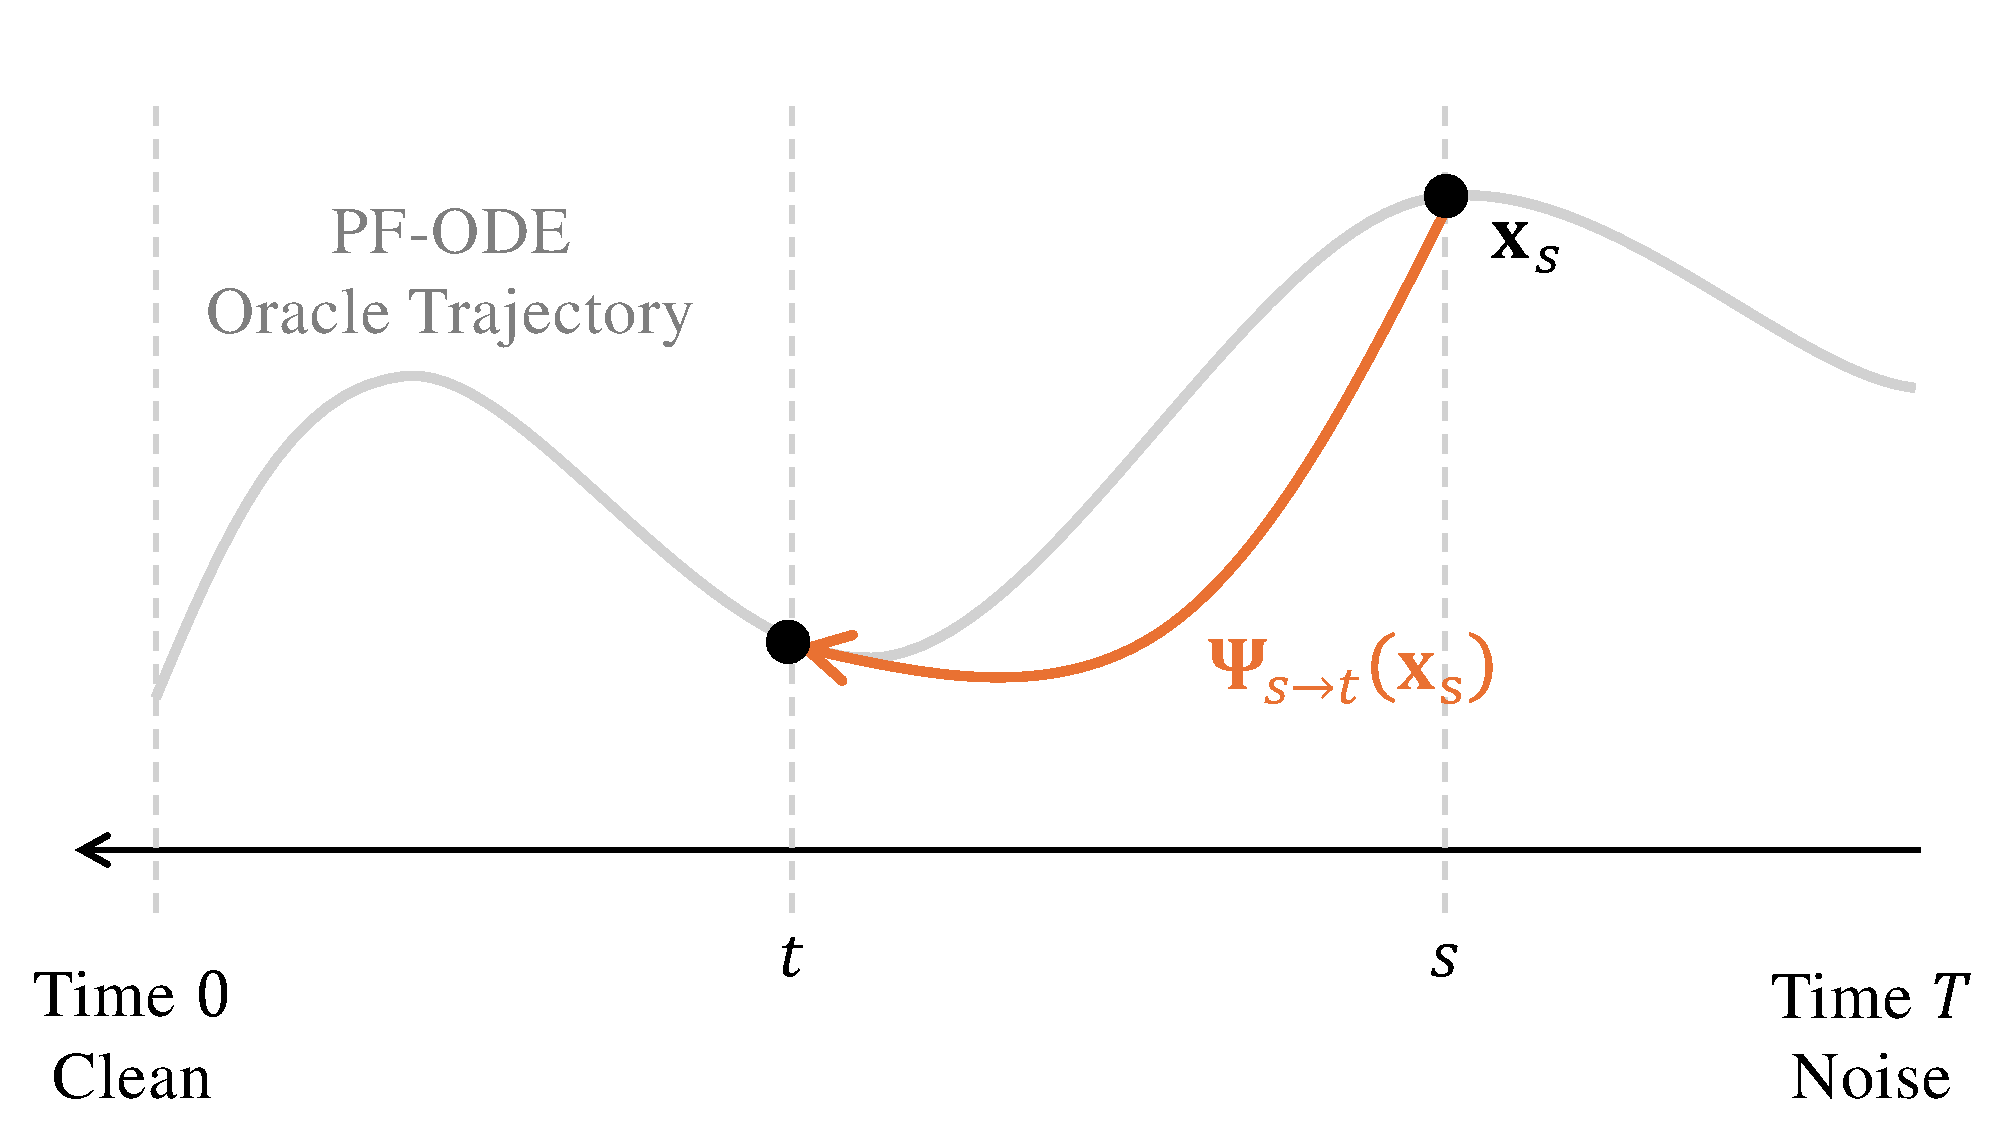
\includegraphics[width=0.9\linewidth]{Images/PartD/flow-map.pdf}
    \caption{\textbfs{流映射的示意图。} 从任意时刻 $s$ 的任意状态 $\rvx_s$ 出发，
流映射 $\bPsi_{s \to t}$ 将其输运到同一 PF-ODE oracle 轨迹上时刻 $t$ 的对应点。\figcredit{由作者绘制。}}
    \label{fig:flow-map-illustration}
\end{figure}


本章围绕一个目标来发展实现该目标的方法，该目标同样支撑着蒸馏，并为流映射的各类公式提供统一视角~\citep{boffi2024flow,hu2025cmt}：
\begin{mdframed}
\begin{equation}\tag{\ref*{eq:general-cm-loss}}\label{eq:general-cm-loss:rep}
  \mathcal{L}_{\mathrm{oracle}}(\btheta)
  := \mathbb{E}_{s,t}\,\mathbb{E}_{\rvx_s \sim p_s}\Big[
     w(s,t)  d\big(\rmG_\btheta(\rvx_s,s,t),  \bPsi_{s\to t}(\rvx_s)\big)
  \Big].
\end{equation}
\end{mdframed}


% Optional: do not consume a new equation number
\addtocounter{equation}{-1}
这里 $s,t$ 从某个时间分布（例如均匀分布）中采样，
$w(s,t) \ge 0$ 为时间对 $(s,t)$ 赋予权重，$d(\cdot,\cdot)$
是某种差异度量，例如 $\ell_2$ 范数的平方。oracle 流映射
$\bPsi_{s\to t}$ 表示这样一种理想变换：取时刻 $s$ 的状态
$\rvx_s$ 并将其直接输运到时刻 $t$：
\[
\bPsi_{s\to t}(\rvx_s) = \rvx_s + \int_s^t \rvv^*(\rvx_u,u)\,\mathrm{d}u,
\]
其中 oracle 漂移项为
\[
\rvv^*(\rvx_u,u) = \E \left[\alpha_u'\rvx_0+ \sigma_u'\beps | \rvx_u\right],
\]
其他等价的参数化也是可行的（见\Cref{ch:all-equivalent}），常见选择包括 $\rvx$-预测和 $\rvv$-预测形式。

在 oracle 损失的最优点处，学习到的模型能够精确恢复真实流映射：
\[
\rmG^*(\rvx_s, s, t) = \bPsi_{s\to t}(\rvx_s), \quad \text{对所有 }\, s,t, \text{ 以及 }\, \rvx_s \sim p_s.
\]


由于流映射 $\bPsi_{s\to t}$ 无法写成闭式，因此必须对其进行近似。
一种选择（已在\Cref{ch:distillation}中讨论）是依赖预训练扩散模型。
或者，正如本章将展示的，可以引入新的、更易处理的代理目标。
为清晰起见，现有方法大致可以根据训练过程是否在循环中查询教师而分类为：
\emph{蒸馏}（显式调用教师模型）和
\emph{从零开始训练}（通过构造自包含的代理目标来避免教师调用）。



基于这一有原则的目标，我们现在转向学习流映射模型的系统性方法，
旨在发展出既实用、又能使生成结果更准确地反映真实数据分布且计算高效的方法。
我们首先对这一范式进行高层次介绍。
\paragraph{特殊流映射：一致性函数。}
\emph{一致性模型}~\citep{song2023consistency} 是流映射学习最早期的开创性方法之一。
它们学习一个少步去噪器 $\rvf_\btheta(\cdot,s)$，用以近似指向原点的流映射这一特殊情形：
\[
\bPsi_{s\to 0}(\cdot), \qquad s \in (0,T].
\]
其核心思想是：每个带噪样本 $\rvx_s$ 都应被映射回其轨迹终点的干净数据点 $\rvx_0$。
形式上，CM 系列~\citep{song2023consistency,songimproved,geng2024consistency,lu2024simplifying} 的 oracle 训练目标为
\begin{align}\label{eq:oracle-cm}
    \mathcal{L}_{\methodl{oracle}{CM}}(\btheta) 
    := \E_{s} \E_{\rvx_s\sim p_s} \left[ w(s)  d \left(\rvf_\btheta(\rvx_s,s), \bPsi_{s\to 0}(\rvx_s)\right)\right].
\end{align}




然而，实践中 oracle $\bPsi_{s\to 0}(\rvx_s)$ 是不可得的。因此它被一个取自同一轨迹上稍早一步 $\bPsi_{s\to s-\Delta s}(\rvx_s)$ 的\emph{停梯度}目标（记为 $\rvf_{\btheta^-}$）所替代：
\[
\bPsi_{s\to 0}(\rvx_s) \approx \rvf_{\btheta^-} \left(\bPsi_{s\to s-\Delta s}(\rvx_s),\,s-\Delta s\right), \quad \Delta s > 0,
\]
其中 $\bPsi_{s\to s-\Delta s}(\rvx_s)$ 本身也必须被近似。有两种
实用的策略：(i) \emph{蒸馏}，依赖预训练扩散模型；(ii) \emph{从零开始训练}，
在无教师引导的情况下使用单点估计。

% \begin{itemize}
%     \item \textbfs{Distillation:} use a one-step solver applied to a pre-trained diffusion model. This approach is called \emph{Consistency Distillation (CD)}.
%     \item \textbfs{From Scratch:} use the analytic one-point estimate
%     \[
%       \rvx_{s-\Delta s} = \alpha_{s-\Delta s}\,\rvx_0 + \sigma_{s-\Delta s}\,\beps,
%     \]
%     with the same $(\rvx_0,\beps)$ as in $\rvx_s = \alpha_s \rvx_0 + \sigma_s \beps$. This approach is called \emph{Consistency Training (CT)}.
% \end{itemize} 


\paragraph{一般流映射。} 两种代表性方法是\emph{一致性轨迹模型}（CTM）和\emph{均值流}（MF）。
\subparagraph{一致性轨迹模型。} \emph{一致性轨迹模型}（CTM）\\~\citep{kim2023consistency} 是首个学习任意起始和终止时刻的一般流映射 $\bPsi_{s\to t}$ 的工作，可以看作是\Cref{eq:general-cm-loss:rep}统一目标下的一个具体实例。CTM 采用受 Euler 启发的参数化，将 oracle 流映射表示为
\begin{align*}
\bPsi_{s\to t}(\rvx_s)
:= \rvx_s + \int_s^t \rvv^*(\rvx_u,u)\diff u 
= \frac{t}{s} \rvx_s
+ \frac{s-t}{s}
\underbrace{\Big[\rvx_s + \frac{s}{s-t} \int_s^t \rvv^*(\rvx_u,u) \diff u\Big]}_{\approx~\rvg_{\btheta}},
\end{align*}
这启发了如下神经参数化
\begin{align}\label{eq:ctm_para_1}
\rmG_{\btheta}(\rvx_s,s,t)
:= \frac{t}{s}\,\rvx_s + \frac{s-t}{s}\,\rvg_\btheta(\rvx_s,s,t),
\end{align}
其中 $\rvg_\btheta$ 是一个神经网络，训练使其满足 $\bPsi_{s\to t}(\rvx_s)\approx \rmG_{\btheta}(\rvx_s,s,t)$。

由于 oracle $\bPsi_{s\to t}(\rvx_s)$ 不可达，CTM 对在中间时刻 $u$ 处求值的\emph{停梯度}目标进行训练：
\[
\bPsi_{s\to t}(\rvx_s)
 \approx
\rmG_{\btheta^-} \big(\bPsi_{s\to u}(\rvx_s),\,u,\,t\big),
\qquad u\in[t,s],
\]
其中中间状态 $\bPsi_{s\to u}(\rvx_s)$ 以两种方式之一进行近似：
(i) \emph{蒸馏}，使用对预训练扩散教师施加的少步求解器；或
(ii) \emph{从零开始训练}，直接通过 $\rmG_\btheta$ 参数化构造自诱导教师。


\subparagraph{均值流。}
均值流（MF）~\citep{geng2025mean} 建立在流匹配之上，对区间 $[t,s]$（$t\le s$）上的\emph{平均漂移}进行建模：
\[
\rvh_{\btheta}(\rvx_s,s,t)
 \approx 
\rvh^*(\rvx_s,s,t)
:= \frac{1}{\,t-s\,}\int_s^t \rvv^*(\rvx_u,u)\,\diff u,
\]
同样与\Cref{eq:general-cm-loss:rep}对齐。
对恒等式
\[
(t-s)\,\rvh^*(\rvx_s,s,t)  =  \int_s^t \rvv^*(\rvx_u,u)\,\diff u
\]
关于 $s$ 求导，得到一个自指关系，由此启发 MF 目标
\[
\mathcal{L}_{\mathrm{MF}}(\btheta)
:= \E_s\,\E_{\rvx_s\sim p_s} \Big[w(s)\,\big\|
\rvh_{\btheta}(\rvx_s,s,t)-\rvh_{\btheta^-}^{\mathrm{tgt}}(\rvx_s,s,t)
\big\|_2^2\Big],
\]
其停梯度目标为
\[
\rvh_{\btheta^-}^{\mathrm{tgt}}(\rvx_s,s,t)
:= \rvv^*(\rvx_s,s)  -  (s-t) \left(\rvv^*(\rvx_s,s)\,\partial_\rvx \rvh_{\btheta^-} + \partial_s \rvh_{\btheta^-}\right).
\]
实践中，oracle 速度 $\rvv^*(\rvx_s,s)$ 也必须被近似。
两种常见策略为：(i) \emph{蒸馏}，利用经流匹配训练的预训练扩散模型；或 (ii) \emph{从零开始训练}，
使用由前向加噪过程 $\rvx_s = \alpha_s \rvx_0+\sigma_s \beps$ 导出的单点条件速度
$\alpha'_s\,\rvx_0+\sigma'_s\,\beps$。



\subparagraph{CTM 与 MF 之间的关系。}
CTM 与 MF 近似的是同一路径积分，但对其参数化了不同的代理目标：
\begin{align*}
\bPsi_{s\to t}(\rvx_s)
&:= \rvx_s  +  \int_s^t \rvv^*(\rvx_u,u)\,\diff u
\\[2pt]
&= \frac{t}{s}\,\rvx_s
 +  \frac{s-t}{s}\,
\underbrace{\Big[\rvx_s + \frac{s}{\,s-t\,} \int_s^t \rvv^*(\rvx_u,u)\,\diff u\Big]}_{\approx~\rvg_{\btheta} }
\\[4pt]
&= \rvx_s  +  (t-s)\,
\underbrace{\Big[\frac{1}{\,t-s\,} \int_s^t \rvv^*(\rvx_u,u)\,\diff u\Big]}_{\approx~\rvh_{\btheta} }.
\end{align*}
换言之，CTM 通过 $\rvg_\btheta$ 学习\emph{斜率位移}，而 MF 学习\emph{平均漂移} $\rvh_\btheta$；两者都是近似定义 $\bPsi_{s\to t}$ 的同一积分的一致方式。


\paragraph{接下来的内容。}
我们从 CM 系列开始，它关注特定的流映射
$\bPsi_{s\to 0}$。这部分既包括其在\Cref{sec:discrete-cm}中的离散时间起源，
也包括在\Cref{sec:conti-cm}中的连续时间扩展。然后我们转向一般流映射，
详细讨论两个关键代表 CTM 和 MF。它们的参数化、训练策略和实用近似分别在
\Cref{sec:CTM}和\Cref{sec:MF}中介绍。

我们指出，\Cref{sec:edm}中介绍的\emph{阐释扩散模型}（EDM）为
设计 $\rvx$-预测模型的网络参数化提供了系统性指南，并在经验上表现出色。
虽然本节可视为可选，但 EDM 公式是 CM 类模型的重要基础。


为便于后续论述清晰，我们不严格遵循这些方法出现的时间顺序。
相反，我们按概念关系来组织讨论。
不过，为承认原创性并尊重时间顺序，我们在\Cref{fig:timeline}中给出历史时间线。




%%%%%%%%%%%%%%%%%%%%%%%%


\clearpage
\newpage


\section{特殊流映射：离散时间一致性模型}\label{sec:discrete-cm}

\paragraph{流映射的一个重要原理：半群性质。}
\begin{figure}[th!]
    \centering
    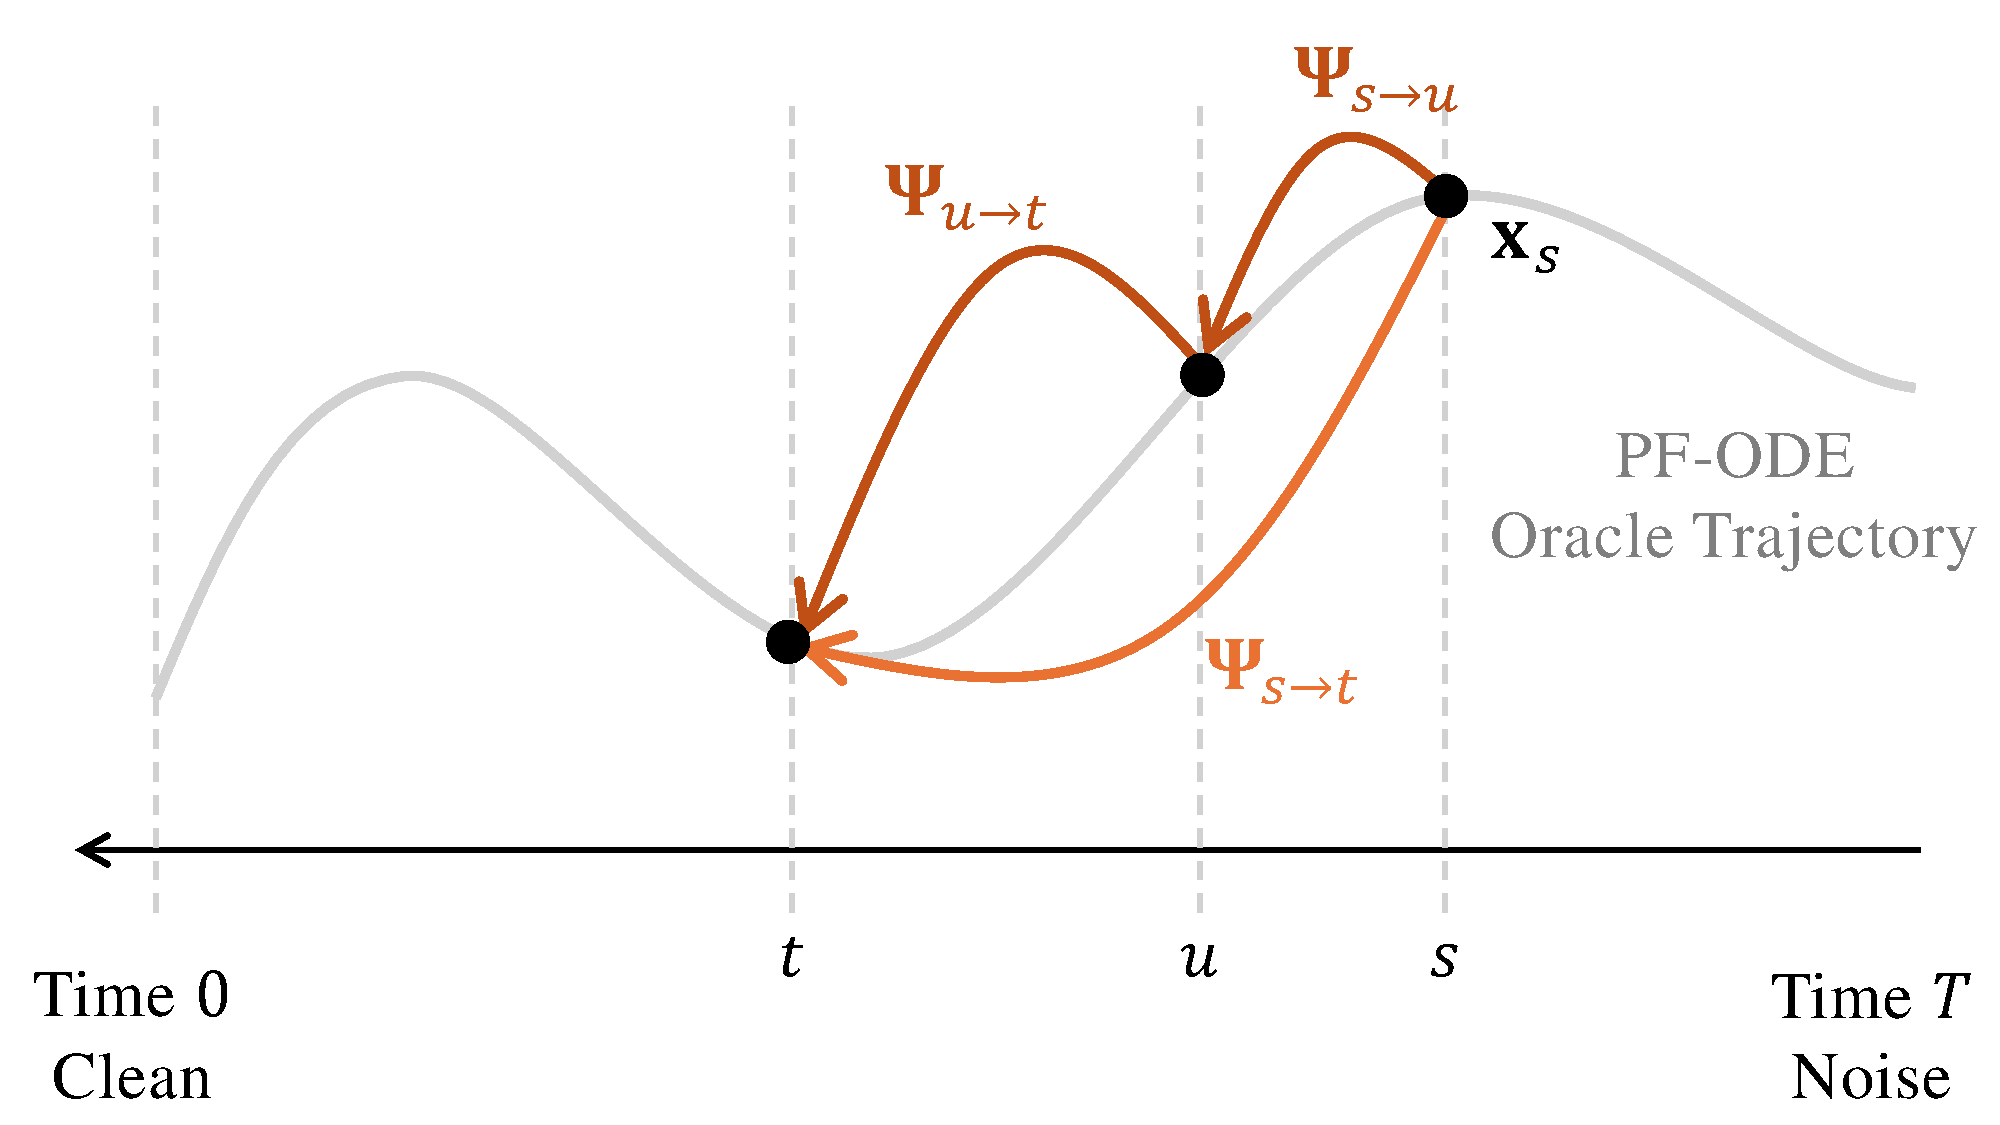
\includegraphics[width=0.9\linewidth]{Images/PartD/semigroup.pdf}
    \caption{\textbfs{流映射半群性质的示意图。}
该性质表明，先从 $s$ 转移到 $u$，再从 $u$ 转移到 $t$，
等价于直接从 $s$ 转移到 $t$。
\figcredit{由作者绘制。}}
    \label{fig:semigroup}
\end{figure}


一致性模型（在\Cref{sec:discrete-cm,sec:conti-cm}中介绍）及其推广——一致性轨迹模型（\Cref{sec:CTM}），都通过利用流映射的一种关键数学结构来定义其回归目标。
这种结构就是基本的\emph{半群性质}：
\begin{mdframed}
   \begin{align}\label{eq:semi-group}
       \bPsi_{u\to t}\circ \bPsi_{s\to u}=\bPsi_{s\to t},
       \,\,\,
       \bPsi_{s\to s}=\rmI, \quad \text{对所有 }\, s, u, t \in [0,T].
   \end{align} 
\end{mdframed}
直观上，这意味着如果我们先将状态从 $s$ 演化到 $u$（通过 $\bPsi_{s\rightarrow u}$），再从 $u$ 演化到 $t$（通过 $\bPsi_{u\rightarrow t}$），最终到达的点与直接从 $s$ 演化到 $t$ 完全相同。
这不过是 ODE 求解的基本原理\footnote{半群性质源自 ODE 初值问题唯一性定理（见\Cref{app:de}）。}：一旦流的起点给定，其未来演化就被完全确定，并遵循唯一明确的路径。无论我们用一大步沿此路径前进，还是将其划分为更小的区间，我们仍然沿同一轨迹移动并到达相同的终点。

为了进一步建立对半群性质的直觉，考虑 PF-ODE 的解轨迹 $\{\rvx(s)\}_{s \in [0,T]}$
\begin{align*}
    \frac{\diff \rvx(\tau)}{\diff \tau} = \rvv^*(\rvx(\tau), \tau),
\end{align*}
其在时刻 $T$ 处给定固定初值 $\rvx(T)$，沿时间向后求解。
若我们将终点时刻固定为 $t=0$，相应的流映射可以更简单地写为
\[
\rvf^*(\cdot, s) := \bPsi_{s\to 0}(\cdot),
\]
称之为\emph{一致性函数}。
按构造，该函数直接从\Cref{eq:semi-group}在 $t=0$ 时的半群恒等式继承了几条基本性质：

\begin{enumerate}
    \item[(i)] \textbfs{全局一致性：}轨迹上的每一点都映射到相同的干净终点，
    \[
       \rvf^*(\rvx(s), s) = \rvx(0), \quad \text{对所有 }\, s \in [0,T].
    \]
    这是因为
\begin{align*}
\rvf^*(\rvx(s),s)
&= \bPsi_{s\to 0}\big(\bPsi_{0\to s}(\rvx(0))\big)
= \big(\bPsi_{s\to 0}\circ \bPsi_{0\to s}\big)(\rvx(0))
\\&= \bPsi_{0\to 0}(\rvx(0))
= \rvx(0).
\end{align*}
    \item[(ii)] \textbfs{自一致性：}同一轨迹上任意两点必须给出相同的输出，
    \begin{align}\label{eq:cm-self-consistency}
       \rvf^*(\rvx(s), s) = \rvf^*(\rvx(u), u), \quad \text{对所有 }\, s, u \in [0,T].
    \end{align}
    这是对半群恒等式的直接重释：$\Psi_{s\rightarrow 0}\circ\Psi_{0\rightarrow s}=\Psi_{u\rightarrow 0}\circ\Psi_{0\rightarrow u}$。
    \item[(iii)] \textbfs{局部一致性：}沿轨迹求值时，一致性函数关于 $s$ 不变，
    \begin{align}\label{eq:cm-diff}
        \frac{\diff}{\diff s}\,\rvf^*(\rvx(s),s) = 0,
        \qquad \rvf^*(\rvx(0),0) = \rvx(0).
    \end{align}
这由全局一致性得到，后者指出 $\rvf^*(\rvx(s), s)$ 沿轨迹不随 $s$ 改变。
\end{enumerate}
这三条性质彼此等价。每一条都表明：沿任意解轨迹 $s\mapsto \rvx(s)$，
流到原点/一致性映射 $\rvf^*(\rvx(s),s)=\bPsi_{s\to 0}(\rvx(s))$
都给出相同的终点 $\rvx(0)$，与起始时刻无关。


\paragraph{一致性模型的目标。}
CM 旨在训练一个神经网络
$\rvf_{\bm{\theta}} \colon \mathbb{R}^D \times [0,T] \to \mathbb{R}^D$
来近似特殊流映射 $\bPsi_{s\to 0}$，即一致性函数\footnote{ODE 的一致性函数概念可推广到 SDE 上满足如下条件的函数
$\rvf(\rvx,t)$：使 $\rvf(\rvx_t,t)$ 成为关于 SDE 自然 $\sigma$-代数流的（局部）鞅，即
\[
\E[\rvf(\rvx_t,t)|\rvx_s]=\rvf(\rvx_s,s),\quad\text{对所有 }\quad t\ge s.
\]
这一推广在\citep{daras2023consistent,lai2023fp}中被提出/观察到，
理论上的联系总结于\citep{lai2023equivalence}。}。
其核心思想是在 PF-ODE 的多条轨迹上强制执行半群性质，确保同一数据点的不同带噪版本一致地映射回相同的干净原点（更确切地说，这对应于\Cref{eq:semi-group}中 $t=0$ 且 $u=s-\Delta s$ 的特殊情形）。

然而，实现这一目标有多种方式。
其选择取决于是否有可用的预训练扩散模型，以及训练是在离散时间还是连续时间体系下进行。
我们先在\Cref{tb:consistency-methods}中概述这些变体，并在\Cref{fig:cd-ct-loss-distill}中示意它们的目标。
随后的几节（\Cref{sec:discrete-cm,sec:conti-cm}）再逐步展开每种方法的细节。

\begin{table}[th]
  \caption{一致性模型的训练目标}
  \small
  \centering
  \resizebox{0.76\textwidth}{!}{
  \begin{tabular}{ccc}
     \toprule
     & \textbfs{蒸馏} & \textbfs{从零开始} \\
     \midrule
     \textbfs{离散时间} & \Cref{eq:cd-discrete-approx-N} & \Cref{eq:ct-discrete-approx-N} \\
     \textbfs{连续时间} & \Cref{eq:cd-continuous-time}  & \Cref{eq:ct-continuous-time} \\
     \bottomrule
  \end{tabular}
  }
  \label{tb:consistency-methods}
\end{table} 




\subsection{学习一致性函数的离散时间近似}\label{subsec:approx-cm}

原则上，可以通过最小化 oracle 损失\Cref{eq:oracle-cm}来学习一致性函数：
\[
    \mathcal{L}_{\methodl{oracle}{CM}}(\btheta)
    := \E_{s} \E_{\rvx_s\sim p_s} \left[ w(s)  d \left(\rvf_\btheta(\rvx_s,s), \bPsi_{s\to 0}(\rvx_s)\right)\right].
\]
该目标强制每个带噪样本 $\rvx_s$ 都被映射回其干净终点 $\bPsi_{s\to 0}(\rvx_s)$。

挑战在于 oracle 映射 $\bPsi_{s\to 0}(\rvx_s)$ 在实践中不可得。
为克服这一点，\citet{song2023consistency} 利用\emph{半群性质}：同一 PF-ODE 轨迹上的任意带噪状态及其相邻步骤必然映射到相同的干净终点。
具体地，oracle 目标被轨迹上稍早一点处的\emph{停梯度}目标所替代：
\begin{align*}
    \bPsi_{s\to 0}(\rvx_s)
    &= \bPsi_{s-\Delta s \to 0} \left(\bPsi_{s\to s-\Delta s}(\rvx_s)\right) \\
    &\approx \rvf_{\btheta^-} \left(\bPsi_{s\to s-\Delta s}(\rvx_s),\,s-\Delta s\right),
    \qquad \Delta s > 0,
\end{align*}
其中 $\bm{\theta}^-$ 是停梯度算子下的参数。
进一步的困难在于，中间状态 $\bPsi_{s\to s-\Delta s}(\rvx_s)$ 同样没有闭式，必须自身被近似。
已提出两种实用体系：

\paragraph{有预训练扩散模型（一致性蒸馏）。}
假设我们可以访问一个预训练的扩散模型。
一致性蒸馏（CD）利用教师模型，通过仅模拟单步反向 ODE 步骤来近似中间状态 $\bPsi_{s\to s-\Delta s}(\rvx_s)$：
\[
 \bPsi_{s\to s-\Delta s}(\rvx_s)  \approx  \mathtt{Solver}_{s \to s-\Delta s}(\rvx_s).
\]

更具体地说，预训练扩散模型提供了得分函数的估计
$\rvs_{\bm{\phi}^\times}(\rvx_s, s) \approx \nabla_{\rvx_s}\log p_s(\rvx_s)$。
利用它，可以从 $\rvx_s$ 执行一步 DDIM 更新，得到 $s' = s-\Delta s$ 处状态的近似：
\begin{align*}
    \bPsi_{s\to s-\Delta s}(\rvx_s) 
    &\approx \frac{\alpha_{s'}}{\alpha_s}\,\rvx_s 
    + \sigma_s^2 \left( \frac{\alpha_{s'}}{\alpha_s} - \frac{\sigma_{s'}}{\sigma_s} \right)\nabla_{\rvx_s}\log p_s(\rvx_s) \\
    &\approx \frac{\alpha_{s'}}{\alpha_s}\,\rvx_s 
    + \sigma_s^2 \left( \frac{\alpha_{s'}}{\alpha_s} - \frac{\sigma_{s'}}{\sigma_s} \right)\rvs_{\bm{\phi}^\times}(\rvx_s, s) \\
    &:= \tilde{\rvx}_{s'}^{\bm{\phi}^\times}.
\end{align*}

将此构造与停梯度目标结合，便得到 oracle 损失 $\mathcal{L}_{\methodl{oracle}{CM}}(\btheta)$ 的实用\emph{离散时间}代理。
形式上，在划分 $0 = s_1 < s_2 < \cdots < s_N = T$ 上，CD 的训练目标为
\begin{mdframed}
\begin{align}\label{eq:cd-discrete-approx-N}
    \mathcal{L}_{\text{CD}}^N(\bm{\theta}, \bm{\theta}^-; \bm{\phi}^\times)
    := \E_{\rvx_0, \beps, i} \Big[\, \omega(s_i)\,
    d\big(\rvf_{\bm{\theta}}(\rvx_{s_{i+1}}, s_{i+1}),\,
          \rvf_{\bm{\theta}^-}(\tilde{\rvx}_{s_i}^{\bm{\phi}^\times}, s_i)\big)\Big].
\end{align}
\end{mdframed}
这里，$\omega(\cdot)$ 是一个时间相关的权重，$d(\cdot,\cdot)$ 是距离度量，$\bm{\theta}^-$ 表示停梯度参数，用于防止塌缩到平凡解（例如常数预测）。



\paragraph{没有预训练扩散模型（一致性训练）。}
当没有可用的预训练扩散模型时，oracle 得分 $\nabla_{\rvx}\log p_s(\rvx_s)$ 仍然可以通过简单的单点近似直接估计（尽管方差较高）。
回忆它具有条件期望形式：
\begin{align*}
    \nabla_{\rvx_s} \log p_s(\rvx_s)
    &= \E_{\rvx_0 \sim p(\rvx_0|\rvx_s)} \left[ \nabla_{\rvx_s}\log p(\rvx_s|\rvx_0) \right] \\
    &= \E_{\rvx_0 \sim p(\rvx_0|\rvx_s)} \left[ -\frac{\rvx_s - \alpha_s \rvx_0}{\sigma_s^2} \right].
\end{align*}
上述恒等式暗示了一个简单的单样本估计器。
若 $\rvx_s$ 是由配对样本 $(\rvx_0,\beps)$ 通过 $\rvx_s = \alpha_s \rvx_0 + \sigma_s \beps$ 得到的，则
\[
\widehat{\nabla_{\rvx}\log p_s}(\rvx_s)
:=-\frac{\boldsymbol\epsilon}{\sigma_s}
=-\frac{\rvx_s-\alpha_s \rvx_0}{\sigma_s^2}
\]
作为 $\rvx_s$ 处得分的一个\emph{无偏}估计器（在给定 $p(\rvx_0|\rvx_s)$ 时条件无偏）。它恰好对应于去噪得分匹配中用作回归目标的\emph{条件得分}。



将该估计代入从 $s$ 到 $s' = s-\Delta s$ 的 DDIM 一步更新（见\Cref{eq:ddim-update-all}）得到
\begin{align}\label{eq:one-pt-score}
\begin{aligned}
    \bPsi_{s\to s'}(\rvx_s)
&\approx
\frac{\alpha_{s'}}{\alpha_s}\,\rvx_s
+ \sigma_s^2 \left(\frac{\alpha_{s'}}{\alpha_s}-\frac{\sigma_{s'}}{\sigma_s}\right)\nabla_{\rvx_s}\log p_s(\rvx_s) && \text{(DDIM)}
\\
&\approx
\frac{\alpha_{s'}}{\alpha_s}\,\rvx_s
+ \sigma_s^2 \left(\frac{\alpha_{s'}}{\alpha_s}-\frac{\sigma_{s'}}{\sigma_s}\right)\widehat{\nabla_{\rvx_s}\log p_s}(\rvx_s) && \text{(单点得分)}
\\
&=
\frac{\alpha_{s'}}{\alpha_s}\,\rvx_s
-\left(\frac{\alpha_{s'}}{\alpha_s}-\frac{\sigma_{s'}}{\sigma_s}\right)(\rvx_s-\alpha_s\rvx_0)
\\
&= \alpha_{s'}\rvx_0+\sigma_{s'}\beps,
\end{aligned}
\end{align}
其中\footnote{最后一个恒等式由前向加噪过程 $\rvx_s=\alpha_s \rvx_0+\sigma_s \beps$ 经初等代数运算直接得到。}
$\rvx_0$ 是相同的数据样本，$\beps$ 是用于构造 $\rvx_s$ 的相同高斯噪声。


由此得到 oracle 目标 $\mathcal{L}_{\methodl{oracle}{CM}}$ 的一个无需教师的离散时间代理，写作
\begin{mdframed}
\begin{align}\label{eq:ct-discrete-approx-N}
    \mathcal{L}_{\text{CT}}^N(\bm{\theta}, \bm{\theta}^-) 
    := \E_{\rvx_0, \beps, i} \left[ 
       \omega(s_i)\, d \left(\rvf_{\bm{\theta}}(\rvx_{s_{i+1}}, s_{i+1}),\, 
       \rvf_{\bm{\theta}^-}(\rvx_{s_i}, s_i)\right)
    \right],
\end{align}
\end{mdframed}
with $\rvx_{s_i} = \alpha_{s_i}\rvx_0 + \sigma_{s_i}\beps$ and $\rvx_{s_{i+1}} = \alpha_{s_{i+1}}\rvx_0 + \sigma_{s_{i+1}}\beps$.

直接用 $\alpha_{s'}\rvx_0+\sigma_{s'}\beps$ 作为 $\bPsi_{s\to s'}(\rvx_s)$ 的近似而不取期望，会引入较高方差\footnote{单点（条件）得分估计 $\widehat{\nabla_{\rvx}\log}p_s(\rvx_s)$ 可视为一个单样本蒙特卡洛估计器，它在给定 $\rvx_s$ 时是\emph{条件无偏}的：在（通常难以处理的）干净后验 $p(\cdot|\rvx_s)$ 上对该估计器求平均可恢复真实得分
\[
\nabla_{\rvx_s}\log p_s(\rvx_s)
= \E_{\rvx_0\sim p(\cdot|\rvx_s)}
 \left[\widehat{\nabla_{\rvx}\log}p_s(\rvx_s)\right].
\]}。
然而，回忆去噪得分匹配中的类似情形（见\Cref{sec:conditional-trick}），其中单个条件得分样本作为训练目标，但一旦在损失中对 $\rvx_0,\beps$ 取平均，便成为无偏的。
同理，$\mathcal{L}_{\mathrm{CT}}^N$ 中对 $\rvx_0$ 和 $\beps$ 的期望会平均掉这种采样噪声，得到无偏的损失级别近似。下面的定理将这种期望级别的论证形式化，以证明单点估计器的合理性。

% The one-point (conditional) score estimate $\widehat{\nabla_{\rvx}\log}p_s(\rvx_s)$ can be viewed as a one-sample Monte Carlo estimator, which is \emph{conditionally unbiased} given $\rvx_s$: averaging this estimator over the (generally intractable) clean posterior $p(\cdot|\rvx_s)$ recovers the true score as
% \[
% \nabla_{\rvx_s}\log p_s(\rvx_s)
% = \E_{\rvx_0\sim p(\cdot|\rvx_s)}
%  \left[\widehat{\nabla_{\rvx}\log}p_s(\rvx_s)\right].
% \]
% If one uses $\alpha_{s'}\rvx_0+\sigma_{s'}\beps$ directly as an approximation of $\bPsi_{s\to s'}(\rvx_s)$ without expectation generally yields high variance. 
% However, after taking the full expectation in the loss (Theorem~\ref{thm:ct-cm}), this one-sample estimator remains unbiased; hence, the one-point score approximation is justified at the loss level.
% In this sense, the update below serves as a practical approximation to the DDIM step computed with an oracle score.
% The following theorem formalizes this expectation-level justification of the one-point estimator.

% and hence,
% \begin{align}
% \begin{aligned}
%     \bPsi_{s\to s'}(\rvx_s)
% &\approx
% \frac{\alpha_{s'}}{\alpha_s}\,\rvx_s 
% + \sigma_s^2 \left(\frac{\alpha_{s'}}{\alpha_s}-\frac{\sigma_{s'}}{\sigma_s}\right)\nabla_{\rvx_s}\log p_s(\rvx_s) && \text{(DDIM)}
% \\
% &=
% \frac{\alpha_{s'}}{\alpha_s}\,\rvx_s 
% + \sigma_s^2 \left(\frac{\alpha_{s'}}{\alpha_s}-\frac{\sigma_{s'}}{\sigma_s}\right) \E_{\rvx_0\sim p(\cdot|\rvx_s)}
%  \left[\widehat{\nabla_{\rvx}\log}p_s(\rvx_s)\right] 
% \\
% &=
% \frac{\alpha_{s'}}{\alpha_s}\,\rvx_s 
% -\left(\frac{\alpha_{s'}}{\alpha_s}-\frac{\sigma_{s'}}{\sigma_s}\right)(\rvx_s-\alpha_s\rvx_0)
% \\
% &=  \E_{\rvx_0\sim p(\cdot|\rvx_s)}
%  \left[\rvx_0+\sigma_{s'}\beps\right]\alpha_{s'}=:\hat\rvx_{s'}, 
% \end{aligned}
% \end{align}




\thmp{CM-CT 在误差 $\mathcal{O}(\Delta s^2)$ 内的等价性}{ct-cm}{
令 $s' := s - \Delta s$，并定义
\begin{align*}
\mathcal{L}_{\mathrm{CM}}(\btheta,\btheta^-)
&:= \E_{s,\rvx_0,\beps} \big[w(s)\,d\big(\rvf_{\btheta}(\rvx_s,s), \rvf_{\btheta^-}(\rvx_{s'}^{\mathrm{DDIM}},s')\big)\big],\\
\mathcal{L}_{\mathrm{CT}}(\btheta,\btheta^-)
&:= \E_{s,\rvx_0,\beps} \big[w(s) d\big(\rvf_{\btheta}(\rvx_s,s), \rvf_{\btheta^-}(\rvx_{s'},s')\big)\big],
\end{align*}
其中
\[
\rvx_{s'}^{\mathrm{DDIM}}
:= \frac{\alpha_{s'}}{\alpha_s}\rvx_s
+ \sigma_s^2 \left(\frac{\alpha_{s'}}{\alpha_s}-\frac{\sigma_{s'}}{\sigma_s}\right)\nabla_{\rvx_s}\log p_s(\rvx_s)
\]
是 oracle DDIM 更新。$\rvx_s = \alpha_s\rvx_0 + \sigma_s\beps$ 和 $\rvx_{s'} = \alpha_{s'}\rvx_0 + \sigma_{s'}\beps$
共享同一对 $(\rvx_0,\beps)$，其中
$\rvx_0 \sim p_{\mathrm{data}}$，且
$\beps \sim \mathcal{N}(\bm{0},\rmI)$。
则
\[
\mathcal{L}_{\mathrm{CM}}(\btheta,\btheta^-)
= \mathcal{L}_{\mathrm{CT}}(\btheta,\btheta^-) + \mathcal{O}(\Delta s^2).
\]
}{首先，注意使用 oracle 得分的 DDIM 更新等于条件均值，
\[
\rvx_{s'}^{\mathrm{DDIM}} = \E[\rvx_{s'} | \rvx_s],
\]
这也可在\Cref{eq:one-pt-score}中对 $p(\cdot|\rvx_s)$ 取期望来验证。
接下来，对
\[
d(\rvf_{\btheta}(\rvx_s,s), \rvf_{\btheta^-}(\cdot,s'))
\]
在 $\rvx_{s'}^{\mathrm{DDIM}}=\E[\rvx_{s'}|\rvx_s]$ 处进行 Taylor 展开。Taylor 展开的线性项消失，因为内层期望在 $\rvx_{s'} | \rvx_s$ 上取，满足 $\E[\rvx_{s'}-\rvx_{s'}^{\mathrm{DDIM}}|\rvx_s]=0$。这表明，通过将条件重新参数化为
$\E_{\rvx_0,\beps|\rvx_s}[\cdot]$，其中
$\rvx_{s'}=\alpha_{s'}\rvx_0+\sigma_{s'}\beps$，
使用单点得分的 DDIM 更新对相同 $(\rvx_0,\beps)$ \emph{逐路径}精确恢复
$\rvx_{s'}$，因此内层期望保持不变。剩余项是二次项，即 $\mathcal{O}(\Delta s^2)$，故 $\mathcal{L}_{\mathrm{CT}}=\mathcal{L}_{\mathrm{CM}}+\mathcal{O}(\Delta s^2)$。
详细的推导见\Cref{app-sec:flow-map}。
}


总之，CD 利用教师模型进行初始化和引导，通常能稳定优化并降低方差。相反，一致性训练（CT）不需要预训练模型，因此可以完全从零开始训练。
尽管存在这一差异，CT 仍可作为完全独立的生成模型。


\paragraph{实践考虑。}
在实践中，\citet{song2023consistency} 采用 \citet{karras2022elucidating} 的 EDM 公式（见\Cref{sec:edm}），前向加噪核为
\[
    \rvx_s = \rvx_0 + s \bm{\epsilon},
\]
并使用其中提出的神经网络参数化
（参见\Cref{eq:D-parametrization}）：
\[
    \rvf_{\bm{\theta}}(\rvx, s)
    = c_{\mathrm{skip}}(s) \rvx
      + c_{\mathrm{out}}(s)\,
        \rmF_{\bm{\theta}} \left(c_{\mathrm{in}}(s)\,\rvx,\, c_{\mathrm{noise}}(s)\right),
\]
其中 $\rmF_{\bm{\theta}}$ 是一个神经网络，系数遵循
\Cref{eq:edm-simple-coefficients}。该参数化具有一个重要的边界性质
\[
    \rvf_{\bm{\theta}}(\rvx, 0) = \rvx,
\]
它在时刻零处强制一致性，并确保网络输出在无噪声时与其输入匹配。





% Assume that $\rvf_{\bm{\theta}}$ learns the optimal trajectory defined by the empirical PF-ODE of the teacher model as in \Cref{eq:teacher-pf-ode}. We revisit \Cref{eq:conti-ct-motivation}  when staying on a trajectory $\{\bar\rvx(s)\}_{s\in[0, T]}$ of the empirical ODE: 
% \begin{align*}
%         &\rvf_{\bm{\theta}^*}(\bar\rvx(s), s) \equiv \bar\rvx(0), \quad \text{for all } s\in [0,T]
%         \\
%         \Leftrightarrow~&\left(\nabla_{\rvx} \rvf_{\bm{\theta}^*}\right)(\bar\rvx(s), s) \cdot 
%     \underbrace{\frac{\diff }{\diff s} \bar\rvx(s)}_{\text{ODE velocity}} + 
%     \left(\frac{\partial }{\partial s} \rvf_{\bm{\theta}^*}\right)(\bar\rvx(s), s) \equiv 0\\
%         \Leftrightarrow~&\left(\nabla_{\rvx} \rvf_{\bm{\theta}^*}\right)(\bar\rvx(s), s) \cdot \rvv_{\bm{\phi}^\times}(\bar\rvx(s), s) + \left(\frac{\partial }{\partial s} \rvf_{\bm{\theta}^*}\right)(\bar\rvx(s), s) \equiv 0
%     \end{align*}

\subsection{使用一致性模型采样}\label{subsec:cm-sampling}
一旦一致性模型 $\rvf_{\bm{\theta}^\times}$ 训练完成，无论是连续时间还是离散时间，都可以用于单步或数步生成样本。算法总结于\Cref{alg:cm_sampling}。

\paragraph{单步生成。} 给定从先验分布采样的初始隐变量 $\hat{\rvx}_T$（实践中为 $\mathcal{N}(\bm{0}, T^2\rmI)$），可通过单次函数求值生成干净样本：
\begin{align*}
    \rvf_{\bm{\theta}^\times}(\hat{\rvx}_T, T).
\end{align*}
\paragraph{多步生成。} 给定预设的时刻序列
\[
T>\tau_1 > \tau_2 > \cdots > \tau_{M-1}=0,
\]
从初始噪声 $\hat\rvx_T$ 出发，在较早时刻通过一致性模型交替进行噪声注入和大跨度干净跳转，逐步精炼样本：
\begin{align*}
    \hat\rvx_T \xrightarrow[\text{得到干净样本}]{\text{长跳}} \rvf_{\bm{\theta}^\times}(\hat{\rvx}_T, T)
    \xrightarrow[\text{到层级 $\tau_1$}]{\text{加噪}} \hat\rvx_{\tau_1}
    \xrightarrow[\text{得到干净样本}]{\text{长跳}} \rvf_{\bm{\theta}^\times}(\hat\rvx_{\tau_1}, \tau_1)
    \xrightarrow[\text{到层级 $\tau_2$}]{\text{加噪}} \cdots.
\end{align*}

\begin{algorithm}[thb!]
    {\small
        \caption{CM 的单步或多步生成采样 \label{alg:cm_sampling}}
    \begin{algorithmic}[1]
        \Require 一致性模型 $\rvf_{\bm{\theta}^\times}(\cdot, \cdot)$，时间点序列 $T>\tau_1 > \tau_2 > \cdots > \tau_{M-1}=0$，初始噪声 $\hat{\rvx}_T$
        \If{单步}
            \State $\rvx \leftarrow \rvf_{\bm{\theta}^\times}(\hat{\rvx}_T, T)$
        \Else
            \State $\rvx \leftarrow \rvf_{\bm{\theta}^\times}(\hat{\rvx}_T, T)$
            \For{$m=1$ \textbf{到} $M-1$}
                \State 采样 $\bm{\epsilon} \sim \mathcal{N}(\bm{0}, \bfI)$
                \State $\hat{\rvx}_{\tau_m} \leftarrow \alpha_{\tau_m}\rvx + \sigma_{\tau_m} \bm{\epsilon}$
                \State $\rvx \leftarrow \rvf_{\bm{\theta}^\times}(\hat{\rvx}_{\tau_m}, \tau_m)$
            \EndFor
        \EndIf
        \Ensure $\rvx$
    \end{algorithmic}
    }
\end{algorithm}














% \subsection{(Optional) Properties of Consistency Function}\label{subsec:consistency-function} 
% CM is motivated by fundamental properties of ODE solution maps, specifically the uniqueness of trajectories once the initial condition is fixed, a classical result from ODE theory.

% Let $\{\rvx(s)\}_{s \in [0, T]}$ denote the solution trajectory of the PF-ODE:
% \begin{align*}
%     \frac{\diff \rvx(\tau)}{\diff \tau} 
%     = f(\tau) \rvx(\tau) - \tfrac{1}{2}g^2(\tau) \nabla_\rvx \log p_\tau(\rvx(\tau)) 
%     =: \rvv^*(\rvx(\tau), \tau),
% \end{align*}
% with some fixed initial condition $\rvx(T)$ at time $T$, solved in reverse time. The oracle consistency function $\rvf^*(\rvx, s):=\bPsi_{s\to 0}(\rvx)$, defined as in \Cref{eq:int_target_gt}, satisfies the following key properties:
% \proppp{Properties of the Solution Map}{cm-sol-map}{
% \begin{enumerate}
%     \item \textbfs{Global Consistency}: $\rvf^*(\rvx(s), s)=\rvx(0)$, for all $s\in[0,T]$.
%     \item \textbfs{Self Consistency}: 
%   \begin{align}\label{eq:cm-self-consistency}
%           \rvf^*(\rvx(s), s)=\rvf^*(\rvx(s'), s'),\quad\text{for any } s, s' \in [0,T].
%   \end{align}
%     \item \textbfs{Local Consistency:}
%     \begin{align}\label{eq:cm-diff}
%         \frac{\diff }{\diff s} \rvf^*(\rvx(s), s) = 0 \quad \text{with} \quad \rvf^*(\rvx(0), 0) = \rvx(0).
%     \end{align}
% \end{enumerate}
% }{These properties directly follow from the semigroup property of the ODE (uniqueness theorem for ODE solutions, commonly known as the Picard-Lindel\"of or Carath\'eodory global existence and uniqueness theorem).}

% It is straightforward to verify that these three properties are actually equivalent. All of these conditions say that: along a given solution trajectory, the solution map yields the same terminal point regardless of the starting time.   


% \rmkb{The concept of a consistency function for an ODE generalizes to a function
% $\rvf(\rvx,t)$ for an SDE such that $\rvf(\rvx_t,t)$ is a (local) martingale with
% respect to the SDE’s natural filtration, i.e.
% \[
% \E[\rvf(\rvx_t,t)|\rvx_s]=\rvf(\rvx_s,s),\quad\text{for all }\quad t\ge s.
% \]
% This generalization was proposed/observed in \citep{daras2023consistent,lai2023fp},
% and the theoretical connections are summarized in \citep{lai2023equivalence}.
% }


% The three equivalent conditions discussed above suggest multiple ways to learn a consistency function. Consistency Models (CM)~\citep{song2023consistency} adopt the \emph{self-consistency property} of \Cref{eq:cm-self-consistency}, which requires that, for any inputs lying on the same ODE solution trajectory, the predicted clean data remains unchanged. We elaborate on this idea in the following subsection, focusing on the distillation-based variant, known as Consistency Distillation (CD).







\clearpage
\newpage

\section{特殊流映射：连续时间一致性模型}\label{sec:conti-cm}

我们现在超越一致性模型的离散时间设定，考虑
连续时间的视角。与固定时间网格并仅在这些采样点上训练的离散方法不同，连续时间公式将
流映射视为对所有时刻均有定义。这一转变消除了对任意离散化的依赖，
并与底层动力学提供了更原则性的对齐。
它还有助于减少由离散化积分自然产生的近似误差，
并确保一致性是全局强制的，而不仅在所选步骤上。

\subsection{连续时间一致性模型}\label{subsec:conti-ct}
为了引出连续时间公式，我们先重温
\Cref{eq:cm-diff}，它描述了可以取时间导数的条件。利用链式法则，我们得到
\begin{align}\label{eq:conti-ct-motivation}
\begin{aligned}
        &\frac{\diff }{\diff s} \rvf^*(\rvx(s), s) = 0 \\
    \Longleftrightarrow\,\,
    &\left(\nabla_{\rvx} \rvf^*\right)(\rvx(s), s) \cdot
    \underbrace{\frac{\diff }{\diff s} \rvx(s)}_{\text{ODE 速度}} +
    \left(\frac{\partial }{\partial s} \rvf^*\right)(\rvx(s), s) = 0,
\end{aligned}
\end{align}
其中轨迹 $\rvx(s)$ 遵循 PF-ODE
\begin{align*}
    \frac{\diff }{\diff s}\rvx(s) =  \rvv^*(\rvx(s), s).
\end{align*}

这一关系表明，一致性函数 $\rvf^*$ 沿 ODE 的任意解轨迹保持为常数。速度场 $\rvv^*$ 在实践中可以从预训练扩散模型估计（当这样的模型可用时），或从直接的单点近似估计，例如
$\alpha_s' \rvx_0 + \sigma_s' \beps$，如
\Cref{sec:discrete-cm}中所解释。

\Cref{eq:conti-ct-motivation}暗示了一种沿 PF-ODE 轨迹一致性的自然连续时间刻画。一种可能的方法是类似于物理信息神经网络（PINN）~\citep{raissi2018deep,boffi2024flow}，通过最小化残差直接强制执行该微分条件：
\begin{align*}
\min_{\bm{\theta}}\mathbb{E}_{s,\rvx_0,\bm{\epsilon}}\left[\left\| \frac{\diff }{\diff s} \rvf_{\bm{\theta}}(\rvx_s, s) \right\|_2^2\right].
\end{align*}

然而在实践中，\citet{song2023consistency,lu2024simplifying} 采用基于教师的一致性目标，而不是直接优化该残差。这促使我们追问：当 $\Delta s \to 0$ 时，离散一致性损失是否存在有意义的无穷小对应物。下面的命题表明，在停梯度目标与在线网络重合的比较点处，缩放后的离散时间梯度收敛到一个连续时间目标的梯度：
\begin{align}\label{eq:cm-discrete}
\mathcal{L}_{\mathrm{CM}}^{\Delta s}(\btheta,\btheta^-)
:= \E \left[\omega(s) \big\|
\rvf_{\btheta}(\rvx_s,s) -
\rvf_{\btheta^-} \big(\bPsi_{s\to s-\Delta s}(\rvx_s), s-\Delta s\big)
\big\|_2^2\right].
\end{align}
% Here, the short-time flow map $\bPsi_{s\to s-\Delta s}(\rvx_s)$ can be
% approximated either with the help of a pre-trained diffusion model
% (i.e., distillation setting) or by a simple one point estimate
% (i.e., training from scratch).
在\Cref{eq:cm-discrete}中取极限 $\Delta s \to 0$ 等价于令\Cref{eq:cd-discrete-approx-N,eq:ct-discrete-approx-N}中
的时间步数 $N \to \infty$。


我们将这一关键思想总结于如下命题。


\proppp{连续时间一致性训练}{continuous-time-ct}{在 $\bm{\theta}=\bm{\theta}^-$ 处成立如下收敛结果：
\begin{align*}
    \left.\lim_{\Delta s\to 0}\frac{1}{\Delta s}\nabla_{\btheta}\mathcal{L}_{\mathrm{CM}}^{\Delta s}(\bm{\theta}, \bm{\theta}^-)\right|_{\bm{\theta}=\bm{\theta}^-}
    =
    \left.\nabla_{\bm{\theta}} \mathcal{L}^\infty_{\mathrm{CM}}(\bm{\theta}, \bm{\theta}^-)\right|_{\bm{\theta}=\bm{\theta}^-}.
\end{align*}
其中
\begin{align*}
    \mathcal{L}^\infty_{\mathrm{CM}}(\bm{\theta},\bm{\theta}^-)
    :=
    \mathbb{E}_{s,\rvx_0,\bm{\epsilon}}\left[
    2\omega(s)\,
    \rvf_{\bm{\theta}}^\top(\rvx_s, s)\cdot
    \frac{\diff }{\diff s}\rvf_{\bm{\theta}^-}(\rvx_s, s)
    \right],
\end{align*}
全微分恒等式为
\begin{align}\label{eq:total-diff}
    \frac{\diff}{\diff s}\rvf_{\btheta^-}(\rvx_s,s)
    =
    \partial_s \rvf_{\btheta^-}(\rvx_s,s)
    + \big(\partial_{\rvx}\rvf_{\btheta^-}(\rvx_s,s)\big)\rvv^*(\rvx_s,s).
\end{align}
}{对停梯度目标在 $(\rvx_s, s)$ 处进行一阶 Taylor 展开表明，损失 $\mathcal{L}_{\mathrm{CM}}^{\Delta s}$ 在 $\mathcal{O}(\Delta s^2)$ 精度内表现为学生更新 $\nabla_{\btheta}\rvf_{\btheta}(\rvx_s,s)$ 与切向变化 $\tfrac{\diff}{\diff s}\rvf_{\btheta^-}(\rvx_s,s)$ 之间的内积。在 $\bm{\theta}=\bm{\theta}^-$ 处求值消除了零阶偏差项，因此缩放后的梯度满足
\[
\left.\lim_{\Delta s\to 0}\frac{1}{\Delta s}\nabla_{\btheta}\mathcal{L}_{\mathrm{CM}}^{\Delta s}\right|_{\bm{\theta}=\bm{\theta}^-}
=
\left.\nabla_{\btheta}\E\left[
2\omega(s)\,
\rvf_{\btheta}^\top(\rvx_s,s)\cdot
\frac{\diff}{\diff s}\rvf_{\btheta^-}(\rvx_s,s)
\right]\right|_{\bm{\theta}=\bm{\theta}^-},
\]
即所证恒等式。我们将证明推迟到\Cref{app-sec:flow-map}。
}

上述结果是在梯度算子
$\nabla_{\bm{\theta}}$ 下书写的，从而包含 $\bm{\theta}^-$ 的项消失，因为
$\bm{\theta}^-$ 在停梯度下被视为常数。注意
$\tfrac{\diff}{\diff s}\rvf_{\btheta^-}(\rvx_s,s)$ 表示沿 oracle 轨迹的全导数，
而非简单的偏时间导数。

总之，连续时间一致性模型可通过最小化如下目标进行训练（忽略因子 $2$）：
\begin{mdframed}
    \begin{align}\label{eq:conti-ct-loss}
    \mathcal{L}^\infty_{\mathrm{CM}}(\bm{\theta},\bm{\theta}^-) := \mathbb{E}_{s,\rvx_0, \bm{\epsilon}}\left[\omega(s)\rvf_{\bm{\theta}}^\top(\rvx_s, s) \cdot \frac{\diff }{\diff s} \rvf_{\bm{\theta}^-}(\rvx_s, s) \right].
\end{align}
\end{mdframed}


\subsection{训练连续时间一致性模型}
与\Cref{subsec:approx-cm}中讨论的离散时间情形类似，
我们现在阐明\Cref{eq:conti-ct-loss}中切向量项的实用近似，
它涉及不可达的 oracle 速度 $\rvv^*$：
\begin{align*}
    \frac{\diff}{\diff s}\rvf_{\btheta^-}(\rvx_s,s)
    = \partial_s \rvf_{\btheta^-}(\rvx_s,s)
    + \big(\partial_{\rvx}\rvf_{\btheta^-}(\rvx_s,s)\big)\,\rvv^*(\rvx_s,s).
\end{align*}
训练完连续时间 CM 后，采样遵循与离散时间情形（\Cref{subsec:cm-sampling}）相同的过程。

\paragraph{连续时间一致性蒸馏。}
若有可用的预训练扩散模型使得
$\rvv_{\bm{\phi}^\times} \approx \rvv^*$，则\Cref{eq:total-diff}中的切向量
$\tfrac{\diff}{\diff s}\rvf_{\btheta^-}(\rvx_s,s)$ 可以用如下代理近似
\begin{align}\label{eq:cd-continuous-time}
    \frac{\diff}{\diff s}\rvf_{\btheta^-}(\rvx_s,s)
     \approx
    \partial_s \rvf_{\btheta^-}(\rvx_s,s)
    + \big(\partial_{\rvx}\rvf_{\btheta^-}(\rvx_s,s)\big)\,
      \rvv_{\bm{\phi}^\times}(\rvx_s,s).
\end{align}
我们将所得目标记为
$\mathcal{L}^\infty_{\mathrm{CM}}(\bm{\theta},\bm{\theta}^-;\bm{\phi}^\times)$。
相应地，命题~\ref{continuous-time-ct} 可以重述为
\[
\lim_{N\to\infty}
N \,\nabla_{\bm{\theta}}\,
\mathcal{L}_{\mathrm{CD}}^{N}(\bm{\theta},\bm{\theta}^-;\bm{\phi}^\times)
  =
\nabla_{\bm{\theta}}\,
\mathcal{L}_{\mathrm{CD}}^{\infty}(\bm{\theta},\bm{\theta}^-;\bm{\phi}^\times).
\]


\paragraph{连续时间一致性训练（从零开始）。} 另一方面，如果没有预训练扩散模型，oracle
速度 $\rvv^*$ 可以用单点条件估计
$\alpha_s'\rvx_0 + \sigma_s'\beps$ 来近似。此时，\Cref{eq:total-diff}中的切向量
$\tfrac{\diff}{\diff s}\rvf_{\btheta^-}(\rvx_s,s)$ 被如下代理替代
\begin{align}\label{eq:ct-continuous-time}
    \frac{\diff}{\diff s}\rvf_{\btheta^-}(\rvx_s,s)
     \approx
    \partial_s \rvf_{\btheta^-}(\rvx_s,s)
    + \big(\partial_{\rvx}\rvf_{\btheta^-}(\rvx_s,s)\big)
      \left(\alpha_s'\rvx_0 + \sigma_s'\beps\right).
\end{align}
我们将所得目标记为
$\mathcal{L}^\infty_{\mathrm{CT}}(\bm{\theta},\bm{\theta}^-)$，对应于
从零开始训练的设定。相应地，
命题~\ref{continuous-time-ct} 可以重述为
\[
\lim_{N\to\infty}
N  \nabla_{\bm{\theta}}
\mathcal{L}_{\mathrm{CT}}^{N}(\bm{\theta},\bm{\theta}^-)
 =
\nabla_{\bm{\theta}}
\mathcal{L}_{\mathrm{CT}}^{\infty}(\bm{\theta},\bm{\theta}^-).
\]



至此，我们已经介绍了列在
\Cref{tb:consistency-methods}中的所有基本方法来实现对一致性
函数 $\bPsi_{s\to 0}$ 的学习。
为了提供更清晰的概览，\Cref{fig:cd-ct-loss-distill}总结了
训练一致性函数的不同损失函数之间的关系。
该图还标注了每种方法是否依赖预训练扩散模型，并区分了连续时间与离散时间目标。




\begin{figure}[ht]
\centering
\scalebox{0.9}{ 
\begin{tikzpicture}[
  box/.style={draw, rounded corners, thick, minimum width=3.5cm, minimum height=1cm, align=center},
  arrow/.style={thick, -{Latex[length=3mm]}},
  xshift=0cm, yshift=0cm
]

% Nodes
\node[box] (discCD) {\small{离散时间 CD}};
\node[box, right=4.5cm of discCD] (discCT) {\small{离散时间 CT}};
\node[box, below=2cm of discCD] (contCD) {\small{连续时间 CD}};
\node[box, below=2cm of discCT] (contCT) {\small{连续时间 CT}};

% Arrows with centered labels
\draw[arrow] (discCD) -- node[midway, above] {\footnotesize 
\shortstack{
$\mathcal{L}_{\text{CD}}(\bm{\theta},\bm{\theta}^-)  =\mathcal{L}_{\text{CT}}(\bm{\theta},\bm{\theta}^-) + \mathcal{O}(\Delta s^2)$
\\
\scriptsize (定理~\ref{thm:ct-cm})
}
} (discCT);
\draw[arrow] (discCD) -- node[midway, left] {
  \footnotesize
  \shortstack{
    $\displaystyle\lim_{N\rightarrow\infty} N \nabla_{\bm{\theta}}\mathcal{L}^N_{\text{CD}}$ \\ $=\nabla_{\bm{\theta}}\mathcal{L}^\infty_{\text{CD}}  $ \\
\scriptsize (定理 5)   
  }
} (contCD);
\draw[arrow] (discCT) -- node[midway, right] {
  \footnotesize
  \shortstack{
    $\displaystyle\lim_{N\rightarrow\infty} N \nabla_{\bm{\theta}}\mathcal{L}^N_{\text{CT}}  $\\
    $= \nabla_{\bm{\theta}}\mathcal{L}^\infty_{\text{CT}}$ \\
\scriptsize (定理 6) 
  }
} (contCT);
\draw[arrow] (discCD) to[out=-30,in=150] node[midway, above, yshift=-8.5mm, text width=5.2cm, align=center] {
  \footnotesize
  \shortstack{
    $\displaystyle\lim_{N\rightarrow\infty} N \nabla_{\bm{\theta}}\mathcal{L}^N_{\text{CD}}(\bm{\theta},\bm{\theta}^-;\bm{\phi}^\times)  $\\
    $= \nabla_{\bm{\theta}}\mathcal{L}^\infty_{\text{CT}}(\bm{\theta},\bm{\theta}^-)$ \\
\scriptsize (定理 6) 
  }
} (contCT);
\draw[arrow] (contCD) -- node[midway, below] {
  \footnotesize
  \shortstack{
    $\mathcal{L}^\infty_{\text{CD}}(\bm{\theta},\bm{\theta}^-;\bm{\phi}^\times)= \mathcal{L}^\infty_{\text{CT}}(\bm{\theta},\bm{\theta}^-)$ 
  }
} (contCT);
\end{tikzpicture}
}
\caption{\textbfs{在 $\ell_2$ 距离度量 $d(\rvx,\rvy)=\|\rvx-\rvy\|_2^2$ 下，离散/连续时间 CD 与 CT 之间关系示意图。} 标注的定理遵循 \citep{song2023consistency} 中的标号。凡涉及 CT 的定理，我们假设得分是完美的：$\rvs_{\bm{\phi}^\times}(\rvx, t) \equiv \nabla_\rvx \log p_t(\rvx)$。$\mathcal{L}^\infty_{\text{CT}}$ 定义于\Cref{eq:conti-ct-loss}，$\mathcal{L}^\infty_{\text{CD}}$ 定义于\Cref{eq:cd-continuous-time}。
\figcredit{由作者绘制。}}
\label{fig:cd-ct-loss-distill}
\end{figure}



然而，切向量
$\tfrac{\diff }{\diff s}\rvf_{\bm{\theta}^-}$
在训练中常导致不稳定。
在随后的可选小节中，我们介绍来自
\emph{简化、稳定化与扩展连续时间一致性模型}
（sCM）~\citep{lu2024simplifying} 的技术来缓解这些问题。





\subsection{(可选) 连续时间一致性训练的实践考虑}
我们的兴趣在于从零开始训练的情形，因为它能产生不依赖外部预训练扩散
模型的独立生成模型。因此，我们将讨论聚焦于连续时间情形。

然而在实践中，直接使用\Cref{eq:conti-ct-loss}训练通常不稳定，
因为项 $\tfrac{\diff}{\diff s}\rvf_{\bm{\theta}^-}$ 可能表现出很大或无界的时间导数，
导致优化时梯度爆炸。为克服这一点，通常需要合适的
参数化和稳定化策略
\citep{geng2025consistency,lu2024simplifying}。正如
\Cref{subsec:summary-disentagle}中所总结，影响稳定
训练的主要因素包括\emph{扩散过程}、\emph{参数化选择}、
\emph{时间加权函数}和\emph{时间采样分布}，所有这些都
在连续时间 CM 中也应被精心设计并解耦。




\paragraph{扩散过程。} 不使用标准扩散参数化
$\rvx_s = \alpha_s \rvx_0 + \sigma_s \bm{\epsilon}$，其中
$\bm{\epsilon} \sim \mathcal{N}(\bm{0}, \rmI)$，
\citet{lu2024simplifying} 采用三角函数调度。
该调度虽然在数学上等价于原始形式
（如\Cref{eq:trig-para}所示），但在训练目标中提供了更清晰的结构和更好的
分离，从而有助于提升训练稳定性
\footnote{直观上，三角函数及其导数都是有界的，这有助于防止 $\frac{\diff}{\diff s} \rvf_{\bm{\theta}^-}$ 等项中的尺度爆炸。详细的讨论见后文。
}。此外，他们纳入了数据分布 $p_{\mathrm{data}}$ 的标准差 $\sigma_{\mathrm{d}}$，与\Cref{subsec:D-design-edm}中 EDM 的设计一致：
\begin{align}\label{eq:trig-scm}
    \rvx_s := \cos(s) \rvx_0 + \sin(s) \rvz, \quad \text{where } \rvz \sim \mathcal{N}(\bm{0}, \sigma_{\mathrm{d}}^2 \rmI).
\end{align}

该公式是完全通用的。对于任意形式为 $\rvx_s = \alpha_s \rvx_0 + \sigma_s \bm{\epsilon}$（其中 $\bm{\epsilon} \sim \mathcal{N}(\bm{0}, \rmI)$）的扩散过程，我们可以等价地写为：
\[
\rvx_s = \alpha_s \rvx_0 + \frac{\sigma_s}{\sigma_\mathrm{d}} \cdot (\sigma_{\mathrm{d}} \bm{\epsilon}),
\]
只需定义 $\rvz := \sigma_{\mathrm{d}} \bm{\epsilon}$，$\alpha'_s := \alpha_s$，$\sigma'_s := \frac{\sigma_s}{\sigma_{\mathrm{d}}}$。然后变换后的对 $(\alpha'_s, \sigma'_s)$ 可用\Cref{eq:any-to-trig}所述的归一化映射为三角形式 $(\cos(s), \sin(s))$。


\paragraph{参数化。}
通过考虑\Cref{subsec:D-design-edm}中 EDM 的类似原理，\citet{lu2024simplifying} 为神经网络提出了如下类似于\Cref{eq:D-parametrization}的参数化：
\begin{align*}
    \rvf_{\bm{\theta}}(\rvx, s) := c_{\mathrm{skip}}(s)\rvx + c_{\mathrm{out}}(s)\rmF_{\bm{\theta}}\left(c_{\mathrm{in}}(s)\rvx, c_{\mathrm{noise}}(s)\right).
\end{align*}
这里，$c_{\mathrm{skip}}(s)$、$c_{\mathrm{out}}(s)$ 和 $c_{\mathrm{in}}(s)$ 可用\Cref{subsec:D-design-edm}中给出的相同准则推导（详细推导见\citet{lu2024simplifying}的附录 B），结果为
\[
c_{\mathrm{skip}}(s) = \cos(s), \quad c_{\mathrm{out}}(s) = -\sigma_{\mathrm{d}} \sin(s), \quad c_{\mathrm{in}}(s) \equiv \frac{1}{\sigma_{\mathrm{d}}}.
\]
这与默认选择 $c_{\mathrm{noise}}(s) = s$ 一并考虑，其中 $\partial_s c_{\mathrm{noise}}(s)$ 是有界的，以确保训练稳定性，如\Cref{eq:ds-decomposition}附近所讨论。这导致三角函数调度下的如下参数化：
\begin{align}\label{eq:trig-nn}
    \rvf_{\bm{\theta}}(\rvx, s) = \cos(s)\rvx - \sin(s)\sigma_{\mathrm{d}}\rmF_{\bm{\theta}}\left(\frac{\rvx}{\sigma_{\mathrm{d}}}, c_{\mathrm{noise}}(s)\right).
\end{align}
我们注意到，该参数化还确保神经网络始终满足边界条件 $\rvf_{\bm{\theta}}(\rvx, 0) \equiv \rvx$（对所有 $\rvx$），这是一致性函数的一个本质属性。



\subparagraph{稳定切向量训练的技术。}
在\Cref{eq:trig-nn}所述的三角函数调度和网络参数化下，\Cref{eq:conti-ct-loss}中损失的梯度变为
\begin{align}\label{eq:conti-ct-loss-trig}
    \nabla_{\bm{\theta}}\mathcal{L}^\infty_{\text{CT}}(\bm{\theta},\bm{\theta}^-)  =\nabla_{\bm{\theta}} \mathbb{E}_{s, \rvx_0, \bm{\epsilon}} \left[ -\omega(s) \sigma_{\mathrm{d}} \sin(s) \rmF_{\bm{\theta}}^\top\left( \frac{\rvx_s}{\sigma_{\mathrm{d}}}, s \right) \cdot \frac{\diff \rvf_{\bm{\theta}^-}}{\diff s} (\rvx_s, s) \right].
\end{align}
 理论上，使用\Cref{eq:conti-ct-loss-trig}中的梯度更新进行训练可能足以学习一致性函数。然而，\citet{lu2024simplifying} 经验观察到，由于切函数的行为，训练过程在实践中可能变得不稳定，切函数为
\begin{align*}
&\underbrace{\frac{\diff \rvf_{\bm{\theta}^-}(\rvx_s, s)}{\diff s}}_{\text{\textbfs{A.}}}
= \\&-\cos(s) \left( \sigma_{\mathrm{d}} \nabla_{\rvx_s} \rmF_{\bm{\theta}^-}\left( \frac{\rvx_s}{\sigma_{\mathrm{d}}}, s \right) - \frac{\diff \rvx_s}{\diff s} \right) - \sin(s) \left( \rvx_s + \sigma_{\mathrm{d}} \frac{\diff \rmF_{\bm{\theta}^-}}{\diff s}\left( \frac{\rvx_s}{\sigma_{\mathrm{d}}}, c_{\mathrm{noise}}(s) \right) \right).
\end{align*}
特别地，在如下项中观察到不稳定
\begin{align*}
\underbrace{\sin(s) \frac{\diff \rmF_{\bm{\theta}^-}}{\diff s}\left( \frac{\rvx_s}{\sigma_{\mathrm{d}}}, c_{\mathrm{noise}}(s) \right)}_{\text{\textbfs{B.}}}
= \sin(s) \nabla_{\rvx_s} \rmF_{\bm{\theta}^-} \frac{\diff \rvx_s}{\diff s}
+ \sin(s) \partial_s \rmF_{\bm{\theta}^-}.
\end{align*}
更具体地说，不稳定性来自如下分量
\begin{align}\label{eq:ds-decomposition}
        \sin(s) \partial_s \rmF_{\bm{\theta}^-} = \sin(s) \underbrace{\frac{\partial c_{\mathrm{noise}}(s)}{\partial s} \cdot \frac{\partial \text{emb}(c_{\mathrm{noise}})}{\partial c_{\mathrm{noise}}}}_{\text{\textbfs{C.}}} \cdot \frac{\partial \rmF_{\bm{\theta}^-}}{\partial \text{emb}(c_{\mathrm{noise}})}.
\end{align}
这里，我们遵循 DM 和 CM 文献中的常见做法，对时间变量 $c_{\mathrm{noise}}(s)$ 应用位置或 Fourier 嵌入，记为 $\text{emb}(\cdot)$：
\[
s \mapsto c_{\mathrm{noise}}(s) \mapsto \text{emb}(c_{\mathrm{noise}}(s)) \mapsto \rmF_{\bm{\theta}^-}\left( \frac{\rvx_s}{\sigma_{\mathrm{d}}}, \text{emb}(c_{\mathrm{noise}}(s)) \right).
\]


因此，引入了一些额外的经验技术来缓解不稳定：
\begin{itemize}
    \item \textbfs{A. 切向量归一化。} 通过用下式替换 $\frac{\diff }{\diff s}\rvf_{\theta^-}$ 来显式归一化切函数
    $    \frac{\frac{\diff }{\diff s} \rvf_{\theta^-}}{\left\| \frac{\diff }{\diff s} \rvf_{\theta^-} \right\|_2 + c}$,
    其中 $c>0$ 是经验设定的常数。或者，将切向量裁剪到 $[-1, 1]$ 也可以有效限制其方差。
    \item \textbfs{B. 切向量预热。} 由于项 $\sin(s)(\rvx_s + \sigma_{\mathrm{d}} \frac{\diff }{\diff s}\rmF_{\bm{\theta}^-})$ 可能引起不稳定，可采用一种可选技术：将系数 $\sin(s)$ 替换为 $r \cdot \sin(s)$，其中 $r$ 在前若干训练迭代中从 0 线性增长到 1。
    \item \textbfs{C. 时间嵌入。} 鉴于\Cref{eq:ds-decomposition}中的导数链，\citet{lu2024simplifying} 选择较小的幅值参数来控制导数 $\frac{\partial \text{emb}(c_{\mathrm{noise}})}{\partial c_{\mathrm{noise}}}$。出于类似原因，选择 $c_{\mathrm{noise}}(s) = s$，其中 $\partial_s c_{\mathrm{noise}}(s)=1$ 是有界常数。
\end{itemize}
除此之外，通常还需要为改善归一化（提升稳定性）以及基于 JVP 高效计算 $\frac{\diff}{\diff s}\rvf_{\theta^-}$ 而做的架构改动，但这超出了我们的讨论范围。

\paragraph{时间加权函数。}
人工设计时间加权函数 $\omega(s)$ 可能导致次优性能。为解决此问题，类似于 EDM-2~\citep{karras2024analyzing} 的做法，\citet{lu2024simplifying} 学习一个自适应加权函数 $\omega_{\bm{\varphi}}(s)$ 来平衡不同时刻 $s$ 的训练损失方差（期望效果见\Cref{eq:effect-adaptive-wgt}）。

进一步阐述，我们观察到\Cref{eq:conti-ct-loss-trig}中的目标函数形式为 
\[
\mathbb{E}_{s, \rvx_0, \bm{\epsilon}} \left[\rmF_{\bm{\theta}}^\top \rvy \right],\quad\text{with}\quad \rvy=-\omega(s) \sigma_{\mathrm{d}} \sin(s)\frac{\diff \rvf_{\bm{\theta}^-}}{\diff s}.
\]
由于 $\rvy$ 是与 $\bm{\theta}$ 无关的向量，\Cref{eq:conti-ct-loss-trig}等价于
\begin{align*}
    \nabla_{\bm{\theta}} \mathbb{E}_{s, \rvx_0, \bm{\epsilon}} \left[\rmF_{\bm{\theta}}^\top \rvy \right]
    = \frac{1}{2} \nabla_{\bm{\theta}} \mathbb{E}_{s, \rvx_0, \bm{\epsilon}} \left\| \rmF_{\bm{\theta}} - \rmF_{\bm{\theta}^-} + \rvy \right\|_2^2.
\end{align*}
基于此观察，\citet{lu2024simplifying} 提出额外训练一个自适应加权网络 $\omega_{\bm{\varphi}}(s)$ 来估计损失范数，表述为如下最小化问题：
\begin{align*}
    \min_{\bm{\varphi}} \mathbb{E}_{s, \rvx_0, \bm{\epsilon}} \left[ \frac{e^{\omega_{\bm{\varphi}}(s)}}{D} \left\| \rmF_{\bm{\theta}} - \rmF_{\bm{\theta}^-} + \rvy \right\|_2^2 - \omega_{\bm{\varphi}}(s) \right].
\end{align*}
为理解自适应加权的效果，注意最优解 $\omega^*(s)$（通过对上述目标关于 $\omega_{\bm{\varphi}}$ 求偏导得到）满足
\begin{align}\label{eq:effect-adaptive-wgt}
    \mathbb{E}_{s, \rvx_0, \bm{\epsilon}} \left[ \frac{e^{\omega^*(s)}}{D} \left\| \rmF_{\bm{\theta}} - \rmF_{\bm{\theta}^-} + \rvy \right\|_2^2 \right] = 1.
\end{align}
即，重新缩放后，不同 $s$ 上期望的（加权）损失保持均匀。因此，自适应加权有效地降低了不同时间步训练损失的方差，带来更均衡、更稳定的训练。

\paragraph{时间采样分布。} \citet{lu2024simplifying} 选择从对数正态提议分布~\citep{karras2022elucidating} 中采样 $\tan(s)$，即
\begin{align}\label{eq:s-dist}
    \log\big(\sigma_{\mathrm{d}} \tan(s)\big) \sim \mathcal{N}(\cdot;P_{\text{mean}}, P_{\text{std}}^2).
\end{align}
这里，$P_{\text{mean}}$ 和 $P_{\text{std}}$ 是两个超参数。


\paragraph{训练目标小结。} 综上，最终的训练损失表示为：
\begin{align*}
    &\mathcal{L}_{\text{sCM}}(\bm{\theta}, \bm{\varphi})
    := \\&\mathbb{E}_{s, \rvx_0, \bm{\epsilon}} \left[
    \frac{e^{\omega_{\bm{\varphi}}(s)}}{D}
    \left\|
    \rmF_{\bm{\theta}}\left(\frac{\rvx_s}{\sigma_{\mathrm{d}}}, s\right)
    - \rmF_{\bm{\theta}^-}\left(\frac{\rvx_s}{\sigma_{\mathrm{d}}}, s\right)
    - \cos(s) \frac{\diff \rvf_{\bm{\theta}^-}}{\diff s}\left(\rvx_s, s\right)
    \right\|_2^2
    - \omega_{\bm{\varphi}}(s)
    \right].
\end{align*}
这里，$s$ 按照\Cref{eq:s-dist}采样，$\rvx_s$ 通过\Cref{eq:trig-scm}计算。用该损失训练得到的模型称为 \emph{sCM}，其训练过程总结于\Cref{alg:scm}。


\begin{algorithm}[tb]
{\small
\caption{连续时间一致性模型 (sCM) 的训练 \label{alg:scm}}
\begin{algorithmic}[1]
\Require 数据集 $\mathcal{D}$，其标准差 $\sigma_{\mathrm{d}}$，预训练 DM $\mathbf{F}_{\text{pretrain}}$（参数 $\bm{\theta}_{\text{pretrain}}$），模型 $\mathbf{F}_{\bm{\theta}}$，加权函数 $\omega_{\boldsymbol{\varphi}}$，学习率 $\eta$，提议 $(P_{\text{mean}}, P_{\text{std}})$，常数 $c$，预热迭代数 $H$
\State \textbfs{初始化：} $\bm{\theta} \gets \bm{\theta}_{\text{pretrain}}$，Iters $\gets 0$
\Repeat
    \State $\rvx_0 \sim \mathcal{D}$，$\mathbf{z} \sim \mathcal{N}(\bm{0}, \sigma_{\mathrm{d}}^2 \mathbf{I})$，$\tau \sim \mathcal{N}(P_{\text{mean}}, P_{\text{std}}^2)$，$s \gets \arctan\left(\frac{e^\tau}{\sigma_{\mathrm{d}}}\right)$
    \State $\rvx_s \gets \cos(s) \rvx_0 + \sin(s) \mathbf{z}$
    \If{一致性训练}
        \State $\frac{\diff\rvx_s}{\diff s} \gets \cos(s) \mathbf{z} - \sin(s) \rvx_0$
    \Else
        \State $\frac{\diff\rvx_s}{\diff s} \gets \sigma_{\mathrm{d}} \mathbf{F}_{\text{pretrain}}\left(\frac{\rvx_s}{\sigma_{\mathrm{d}}}, s\right)$
    \EndIf
    \State $r \gets \min\left(1, \frac{\text{Iters}}{H}\right)$ \hfill \Comment{ 切向量预热}
    \State $\rvw \gets - \cos^2(s) (\sigma_{\mathrm{d}} \mathbf{F}_{\bm{\theta}}^{-} - \frac{\diff\rvx_s}{\diff s}) - r  \cos(s) \sin(s) \left(\rvx_s + \sigma_{\mathrm{d}} \frac{\diff\mathbf{F}_{\bm{\theta}^-}}{\diff s}\right)$
    \State $\rvw \gets \frac{\rvw}{\|\rvw\| + c}$ \hfill \Comment{ 切向量归一化}
    \State $\mathcal{L}_{\text{sCM}}(\bm{\theta}, \boldsymbol{\varphi}) \gets\frac{e^{\omega_{\boldsymbol{\varphi}}(s)}}{D} \norm{ \mathbf{F}_{\bm{\theta}}\left( \frac{\rvx_s}{\sigma_{\mathrm{d}}}, s\right) - \mathbf{F}_{\bm{\theta}^{-}}\left( \frac{\rvx_s}{\sigma_{\mathrm{d}}}, s\right) - \rvw }^2_2 - \omega_{\boldsymbol{\varphi}}(s)$
    \Statex  \hfill \Comment{ 自适应加权}
    \State $(\bm{\theta}, \boldsymbol{\varphi}) \gets (\bm{\theta}, \boldsymbol{\varphi}) - \eta \nabla_{\bm{\theta}, \boldsymbol{\varphi}} \mathcal{L}_{\text{sCM}}(\bm{\theta}, \boldsymbol{\varphi})$
    \State Iters $\gets$ Iters + 1
\Until{收敛}
\end{algorithmic}
}
\end{algorithm}



% \newpage

% \subsection{Comparison of Diffusion Model and Consistency Model.}




% \paragraph{Comparison in Terms of Training Target.} We may conceptually compare the training targets of the Diffusion Model and CM.  

% \begin{itemize}
%     \item \textbfs{Diffusion Model:} A diffusion model trains a neural network to learn the velocity $\rvv^*$ (or equivalently, one of the parametrizations introduced in \Cref{subsec:four-equiv-para}) of an ODE, ensuring that its solution follows the same marginal distribution as the predefined forward transition $\rvx_t = \alpha_t \rvx_0 + \sigma_t \bm{\epsilon}$:
%     \begin{align*}
%         \frac{\diff }{\diff \tau} \rvx(\tau)= \rvv^*\left(\rvx(\tau), \tau\right).
%     \end{align*}
    
%     \item \textbfs{Consistency Model:} A CM directly learns the solution map $\mathbf{f}^*$ of the above ODE:
%     \begin{align*}
%         \mathbf{f}^*(\rvx_{s}, s)
%         \coloneqq \rvx_{s} + \int_{s}^{0} \rvv^*(\rvx_\tau, \tau) \diff \tau.
%     \end{align*}    
% \end{itemize}

% \paragraph{Example.} To illustrate the behavior of different parameterizations and the resulting consistency function, we consider a toy example where the data distribution is given by $p_{\mathrm{data}} = \mathcal{N}(\bm{\mu}_{\mathrm{d}}, \sigma_{\mathrm{d}}^2 \rmI)$, which admits closed-form expressions. For simplicity, we adopt the EDM noise schedule with $\alpha_t = 1$ and $\sigma_t = t$.


% \subparagraph{Marginal Density.} The marginal density $p_t(\rvx):=p_{\mathrm{data}} \circledast \mathcal{N}(\bm{0}, t^2\rmI)$ of the perturbation kernel $\rvx_t=\rvx_0+t\bm{\epsilon}$ is computed as
%     \[
%     \mathcal{N}\left(\bm{\mu}_{\mathrm{d}}, (t^2+\sigma_{\mathrm{d}}^2)\rmI\right).
%     \]
    
% \subparagraph{PF-ODE.} In our case, the PF-ODE is given by  
%     \[
%     \frac{\diff\rvx(t)}{\diff t} = -t \rvs^*\left(\rvx(t), t\right),
%     \]
%     where the score function can be computed analytically as:  
%     \[
%     \rvs^*(\rvx, t) = - \frac{(\rvx - \bm{\mu}_{\mathrm{d}})}{\sigma_{\mathrm{d}}^2 + t^2}.
%     \] 

% \subparagraph{Training Targets.} The four equivalent training targets of the diffusion model and the consistency function can all be computed analytically:
%     \begin{itemize}
%         \item \textbfs{Score}:
%         \[
%         \rvs^*(\rvx_t,t) = -  \frac{(\rvx - \bm{\mu}_{\mathrm{d}})}{\sigma_{\mathrm{d}}^2 + t^2}
%         \]
        
%         \item \textbfs{Noise}:
%         \[
%         \bm{\epsilon}^*(\rvx_t,t) = t \frac{(\rvx - \bm{\mu}_{\mathrm{d}})}{\sigma_{\mathrm{d}}^2 + t^2}
%         \]
        
%         \item \textbfs{Clean}:
%         \[
%         \rvx^*(\rvx_t,t) = \rvx_t - t^2 \frac{(\rvx - \bm{\mu}_{\mathrm{d}})}{\sigma_{\mathrm{d}}^2 + t^2}
%         \]
        
%         \item \textbfs{Velocity}:
%         \[
%         \rvv^*(\rvx_t,t) = t \frac{(\rvx - \bm{\mu}_{\mathrm{d}})}{\sigma_{\mathrm{d}}^2 + t^2}
%         \]
        
%         \item \textbfs{Consistency Function}:     We can solve this ODE analytically by starting with the initial condition $ \rvx(t) = \rvx_t $ and reversing in time to $ t = 0 $, yielding the solution at time $ 0 $:

% \[
% \bm{\mu}_{\mathrm{d}} + (\rvx_t - \bm{\mu}_{\mathrm{d}}) \cdot \frac{\sigma_{\mathrm{d}}}{\sqrt{\sigma_{\mathrm{d}}^2 + t^2}}.
% \]

% Thus, the consistency function is given by:

% \[
% \rvf^*(\rvx_t, t) = \bm{\mu}_{\mathrm{d}} + (\rvx_t - \bm{\mu}_{\mathrm{d}}) \cdot \frac{\sigma_{\mathrm{d}}}{\sqrt{\sigma_{\mathrm{d}}^2 + t^2}}.
% \]

%     \end{itemize}




\clearpage
\newpage

\section{\texorpdfstring{一般流映射：一致性轨迹模型}{General Flow Map: Consistency Trajectory Model}}\label{sec:CTM}

一致性轨迹模型（CTM）~\citep{kim2023consistency} 是首批学习\emph{一般}流映射 $\bPsi_{s\to t}$ 的方法之一。



\paragraph{实践中 CTM 的设定。}
与 CM 系列类似，CTM 最初遵循 EDM~\citep{karras2022elucidating} 的公式（\Cref{sec:edm}），
采用 $\rvx$-预测形式的 PF-ODE，噪声调度为
$\alpha_t = 1$ 且 $\sigma_t = t$。
在此设定下，PF-ODE 变为
\begin{align*}
    \frac{\diff \rvx(\tau)}{\diff \tau}
    = \frac{\rvx(\tau) - \E[\rvx|\rvx(\tau)]}{\tau}.
\end{align*}
从时刻 $s$ 的 $\rvx_s$ 出发演化到较晚的时刻 $t \le s$，
相应的流映射（解）可以等价写为
\begin{align*}
\rvx_s + \int_s^t
    \frac{\rvx_\tau - \E[\rvx |\rvx_\tau]}{\tau}\, \diff \tau.
\end{align*}

CTM 采用受 Euler 启发的参数化：
对 PF-ODE 应用单步 Euler 求解器（等价于 DDIM；见\Cref{eq:ctm-formulation}）得到
\[
\rvx_{s\to t}^{\mathrm{Euler}}
= \rvx_s - (s-t)\,\frac{\rvx_s - \E[\rvx|\rvx_s]}{s}
= \frac{t}{s}\,\rvx_s + \Big(1 - \frac{t}{s}\Big)\E[\rvx|\rvx_s],
\]
其中 $\rvx_{s\to t}^{\mathrm{Euler}}$ 在给定时刻 $s$ 状态 $\rvx_s$ 下近似时刻 $t$ 的解。

虽然 EDM 设定提供了一个简单的说明性案例，
CTM 允许由任意线性高斯前向核 $(\alpha_t, \sigma_t)$ 定义的更一般的噪声调度，
并将 PF-ODE 表示为 $\rvv$-预测形式：
\[
\bPsi_{s\to t}(\rvx_s)
= \rvx_s + \int_s^t \rvv^*(\rvx_u,u) \diff u.
\]
在下文的讨论中，我们聚焦于这一一般公式。


\subsection{用于灵活转移学习的 CTM 参数化}
遵循上述 PF-ODE 的单步 Euler 求解器，
CTM 将 oracle 流映射 $\bPsi_{s\to t}$
重写为输入 $\rvx_s$ 与残差函数 $\rvg^*$ 的凸组合：
\begin{align*}
\bPsi_{s\to t}(\rvx_s)
:= \rvx_s + \int_s^t \rvv^*(\rvx_u,u) \diff u 
= \frac{t}{s}\,\rvx_s
+ \frac{s-t}{s}
\underbrace{\Big[\rvx_s + \frac{s}{s-t} \int_s^t \rvv^*(\rvx_u,u) \diff u\Big]}_{=:~\rvg^*}.
\end{align*}
其中残差项 $\mathbf{g}^*$ 定义为
\begin{align}\label{eq:ctm-g-oracle}
\mathbf{g}^*(\mathbf{x}_{s}, s, t) &:= \rvx_s + \frac{s}{s-t} \int_s^t \rvv^*(\rvx_u,u)\diff u.
\end{align}
\proppp{$\rvg^*$ 的性质}{ctm-g-para}{\begin{enumerate}
    \item[(i)] \textbfs{恢复扩散模型：}
    \[
    \rvg^*(\rvx_s, s, s)=\lim_{t\rightarrow s}\mathbf{g}^*(\mathbf{x}_{s},s,t)=\rvx_s - s\rvv^*(\rvx_s,s).
    \]
    \item[(ii)] \textbfs{积分表示：}
    \[
    \mathbf{g}^*(\mathbf{x}_{s},s,t)=\rvx_s - s\rvv^*(\rvx_s,s)+\mathcal{O}(\vert t-s\vert).
    \]
\end{enumerate}}{由 $\rvg^*$ 的定义，我们得到
\begin{align*}
    \lim_{t\rightarrow s}\mathbf{g}^*(\mathbf{x}_{s},s,t)=\mathbf{x}_{s}-s\lim_{t\rightarrow s}\frac{1}{t-s}\int_{s}^{t}\rvv^*(\mathbf{x}_{\tau}, \tau)\diff \tau=\rvx_s - s\rvv^*(\rvx_s,s).
\end{align*}
 这证明了第一个恒等式。对于第二个论断，由 Taylor 展开有
\begin{align*}
    \mathbf{g}^*(\mathbf{x}_{s},s,t)&=\mathbf{x}_{s}-\frac{s}{s-t}\int_{t}^{s}\rvv^*(\rvx_\tau, \tau)\diff \tau\\
    &=\mathbf{x}_{s}-\frac{s}{s-t}\bigg[ (s-t)\rvv^*(\rvx_s, s) + \mathcal{O}((t-s)^{2}) \bigg]\\
    &=\rvx_s - s\rvv^*(\rvx_s,s)+\mathcal{O}(\vert t-s\vert).
\end{align*}}
由该命题，我们可以得出结论
\begin{enumerate}
    \item 估计 $\rvg^*$ 不仅能近似有限的 $s$ 到 $t$ 转移（对 $s \le t$），还能近似以瞬时速度 $\rvv^*$ 表征的\emph{无穷小} $s$ 到 $s$ 转移。
    \item $\mathbf{g}^*(\mathbf{x}_{s},s,t)$ 可解释为 oracle 速度 $\rvv^*$ 加上 Taylor 展开的残差项。
\end{enumerate}
因此，通过利用\Cref{eq:ctm_para_1}中 CTM 的参数化，学习 $\mathbf{G}_{\bm{\theta}} \approx \bPsi_{s\to t}$（或等价地 $\mathbf{g}_{\bm{\theta}} \approx \mathbf{g}^*$）既能通过 $\mathbf{G}_{\bm{\theta}}$ 实现长跳能力，又能通过 $\mathbf{g}_{\bm{\theta}}$ 恢复扩散模型的速度（或等价地得分函数/去噪器）。因此，该参数化是关键：通过学习 $\mathbf{g}^*$，CTM 在单一框架下统一了扩散模型和一致性模型（特殊流映射）的优势。


在下两节中，我们先介绍 CTM 的一致性损失
（\Cref{subsec:ctm-consistency}），它同时支持蒸馏和
从零开始训练，并通过强制半群性质来实现
$\mathbf{G}_{\bm{\theta}}(\cdot, s, t) \approx \bPsi_{s\to t}(\cdot, s, t)$。
随后描述自然由\Cref{eq:ctm_para_1}参数化产生的辅助损失
（\Cref{subsec:ctm-auxiliary}），包括扩散模型损失和
GAN 损失，它们能显著进一步提升 CTM 的性能。


\subsection{CTM 中的一致性损失}\label{subsec:ctm-consistency}
CTM 旨在近似 oracle 解映射
\[
\mathbf{G}_{\bm{\theta}}(\cdot, s, t) \approx \bPsi_{s\to t}(\cdot, s, t),
\]
对任意 $s \ge t$。由于 oracle $\bPsi_{s\to t}$ 通常没有
闭式，CTM 通过强制\emph{半群性质}（\Cref{eq:semi-group}）来构造可行的回归目标：对任意 $s \ge u \ge t$，
\[
\bPsi_{u\to t}\circ \bPsi_{s\to u} = \bPsi_{s\to t}.
\]
取决于是否有可用的预训练扩散模型，
流映射 $\bPsi_{s\to t}$ 可以用不同方式近似。
贯穿全文，我们假设 $s \ge u \ge t \in [0,T]$。


\paragraph{通过蒸馏训练。}
假设可以访问一个产生
$\rvv_{\bm{\phi}^\times}(\rvx_s, s) \approx \rvv^*(\rvx_s, s)$ 的预训练扩散模型。那么
PF-ODE 由经验动力学近似
\begin{align}
\frac{\diff \rvx(\tau)}{\diff \tau}
= \rvv_{\bm{\phi}^\times}(\rvx_\tau, \tau).
\end{align}
CTM 训练 $\mathbf{G}_{\bm{\theta}}$ 去匹配施加于该经验
ODE 的数值求解器
$\mathtt{Solver}_{s\to t}(\rvx_s;\bm{\phi}^\times)$，它作为 oracle 的可计算代理：
\[
\mathbf{G}_{\bm{\theta}}(\rvx_s, s, t)
\approx \mathtt{Solver}_{s\to t}(\rvx_s;\bm{\phi}^\times)
\approx \bPsi_{s\to t}(\rvx_s, s, t).
\]
拥有强教师时，求解器可在离散化误差内恢复 $\bPsi_{s\to t}$，因此最优学生能紧密匹配真值
（见 \citep{kim2023consistency}，命题 3 和 4）。

然而，当 $s$ 和 $t$ 相距较远时，在训练循环中对整个区间 $[t,s]$ 求解可能代价高昂。为提高效率并提供更平滑的信号，CTM 引入了
\emph{软一致性匹配}，将半群性质付诸实践。
如\Cref{fig:ill_models}所示，CTM 在时刻
$t$ 比较两个预测：学生直接输出 $\mathbf{G}_{\bm{\theta}}(\rvx_s, s, t)$，以及一条混合教师-学生路径，该路径先让教师从 $s$ 推进到随机
$u \sim \mathcal{U}[t,s)$，再让学生从 $u$ 跳到 $t$：
\[
\mathbf{G}_{\bm{\theta}^-} \big(\mathtt{Solver}_{s\to u}(\rvx_s;\bm{\phi}^\times),\, u,\, t\big).
\]
学生被训练去匹配这一组合预测：
\begin{align}\label{eq:soft}
\underbrace{\mathbf{G}_{\bm{\theta}}(\rvx_s, s, t)}_{\approx\, \bPsi_{s\to t}(\rvx_s)}
 \approx
\underbrace{\mathbf{G}_{\bm{\theta}^-} \big(\mathtt{Solver}_{s\to u}(\rvx_s;\bm{\phi}^\times), u, t\big)}_{\approx\, \bPsi_{u\to t}(\bPsi_{s\to u}(\rvx_s))},
\end{align}
其中 $\bm{\theta}^-$ 是 $\mathbf{G}_{\bm{\theta}}$ 的停梯度副本。

通过变化 $u$，CTM 在全局与局部监督之间插值：
\begin{itemize}
    \item \textbfs{全局一致性}（$u = s$）：学生在整个区间 $(t,s)$ 上模仿教师，
    接收信息量最大的教师信号。
    \item \textbfs{局部一致性}（$u = s - \Delta s$）：学生从 $s$ 附近的一个短教师步学习；
    当 $t=0$ 时，这退化为一致性蒸馏。
\end{itemize}

为在对齐轨迹的同时强化样本质量，两个预测都
被停梯度学生映射到时刻 $0$，并在特征空间度量 $d$ 中比较：
\begin{align*}
\rvx_{\mathrm{est}}(\rvx_s,s,t) &:= \mathbf{G}_{\bm{\theta}^-} \big(\mathbf{G}_{\bm{\theta}}(\rvx_s,s,t),\, t,\, 0\big),\\
\rvx_{\mathrm{target}}(\rvx_s,s,u,t) &:= \mathbf{G}_{\bm{\theta}^-} \big(
\mathbf{G}_{\bm{\theta}^-}(\mathtt{Solver}_{s\to u}(\rvx_s;\bm{\phi}^\times), u, t),\, t,\, 0\big).
\end{align*}
CTM 一致性损失为
\begin{mdframed}
    \begin{align}\label{eq:ctm-consist-distill}
\begin{aligned}
\mathcal{L}_{\mathrm{consist}}(\bm{\theta}; \bm{\phi}^\times)
:=
\mathbb{E}_{s \in [0,T]}\mathbb{E}_{t \in [0,s]}\mathbb{E}_{u \in [t,s)}
\mathbb{E}_{\rvx_0}\mathbb{E}_{\rvx_s |\rvx_0}
\Big[ d\big(\rvx_{\mathrm{est}}, \rvx_{\mathrm{target}}\big) \Big],
\end{aligned}
\end{align}
\end{mdframed}
它鼓励学生匹配经验 PF-ODE 解同时
保持生成质量。


\paragraph{从零开始训练。}
利用 CTM 的特殊参数化（命题~\ref{ctm-g-para}(i)），
\[
\rvg^*(\rvx_\tau, \tau, \tau)
= \rvx_\tau - \tau\,\rvv^*(\rvx_\tau,\tau)
 \implies
\rvv^*(\rvx_\tau,\tau)
= \frac{\rvx_\tau - \rvg^*(\rvx_\tau, \tau, \tau)}{\tau}.
\]
因此，我们可以对 $\tau \in [0,T]$ 用 CTM 自身的估计
$\rvg_{\bm{\theta}^-}(\cdot,\tau,\tau)$ 替换 oracle 残差函数
$\rvg^*(\cdot,\tau,\tau)$，
从而得到一个自诱导的经验 PF-ODE：
\begin{align}\label{eq:emp-pf-ode-ctm}
\frac{\diff \rvx(\tau)}{\diff \tau}
= \frac{\rvx(\tau) - \rvg_{\bm{\theta}^-} \left(\rvx(\tau),\tau,\tau\right)}{\tau}.
\end{align}

然后我们通过求解该 ODE 并训练
学生匹配求解器输出来近似 oracle 解映射：
\[
\mathbf{G}_{\bm{\theta}}(\rvx_s, s, t)
\approx \mathtt{Solver}_{s\to t}(\rvx_s;\bm{\theta}^-)
\approx \bPsi_{s\to t}(\rvx_s, s, t).
\]

与蒸馏情形\Cref{eq:soft}类似，当 $s$ 和 $t$ 相距较远时，对 $[t,s]$ 全程积分代价高昂。CTM 因此强制半群
性质以获得更短的监督路径：
\[
\underbrace{\mathbf{G}_{\bm{\theta}}(\rvx_s, s, t)}_{\approx\, \bPsi_{s\to t}(\rvx_s)}
 \approx
\underbrace{\mathbf{G}_{\bm{\theta}^-} \big(\mathtt{Solver}_{s\to u}(\rvx_s;\bm{\theta}^-),\, u,\, t\big)}_{\approx\, \bPsi_{u\to t}(\bPsi_{s\to u}(\rvx_s))},
\]
其中 $u \sim \mathcal{U}[t,s)$，$\bm{\theta}^-$ 是学生的停梯度副本。与蒸馏的唯一
不同是外部教师
$\rvv_{\bm{\phi}^\times}$ 被自诱导教师
$\rvg_{\bm{\theta}^-}$ 所替代。

为将轨迹匹配与样本质量耦合，两个预测都用
停梯度学生映射到时刻 $0$ 并在特征空间比较。无任何
预训练模型时的目标为
\[
\hat{\rvx}_{\mathrm{target}}
:= \mathbf{G}_{\bm{\theta}^-} \big(
\mathbf{G}_{\bm{\theta}^-}(\mathtt{Solver}_{s\to u}(\rvx_s;\bm{\theta}^-),\, u,\, t),\, t,\, 0\big),
\]
它替换\Cref{eq:ctm-consist-distill}中的 $\rvx_{\mathrm{target}}$，并给出：
\begin{mdframed}
    \begin{align}\label{eq:ctm-consist-scratch}
\begin{aligned}
\mathcal{L}_{\mathrm{consist}}(\bm{\theta}; \btheta^-)
:=
\mathbb{E}_{s \in [0,T]}\mathbb{E}_{t \in [0,s]}\mathbb{E}_{u \in [t,s)}
\mathbb{E}_{\rvx_0}\mathbb{E}_{\rvx_s |\rvx_0}
\Big[ d\big(\rvx_{\mathrm{est}}, \hat\rvx_{\mathrm{target}}\big) \Big],
\end{aligned}
\end{align}
\end{mdframed}
从概念上讲，这是
CTM 内的自蒸馏：模型提供自身的短时程教师
信号，同时学生学习完整转移。


\begin{figure}
    \centering
    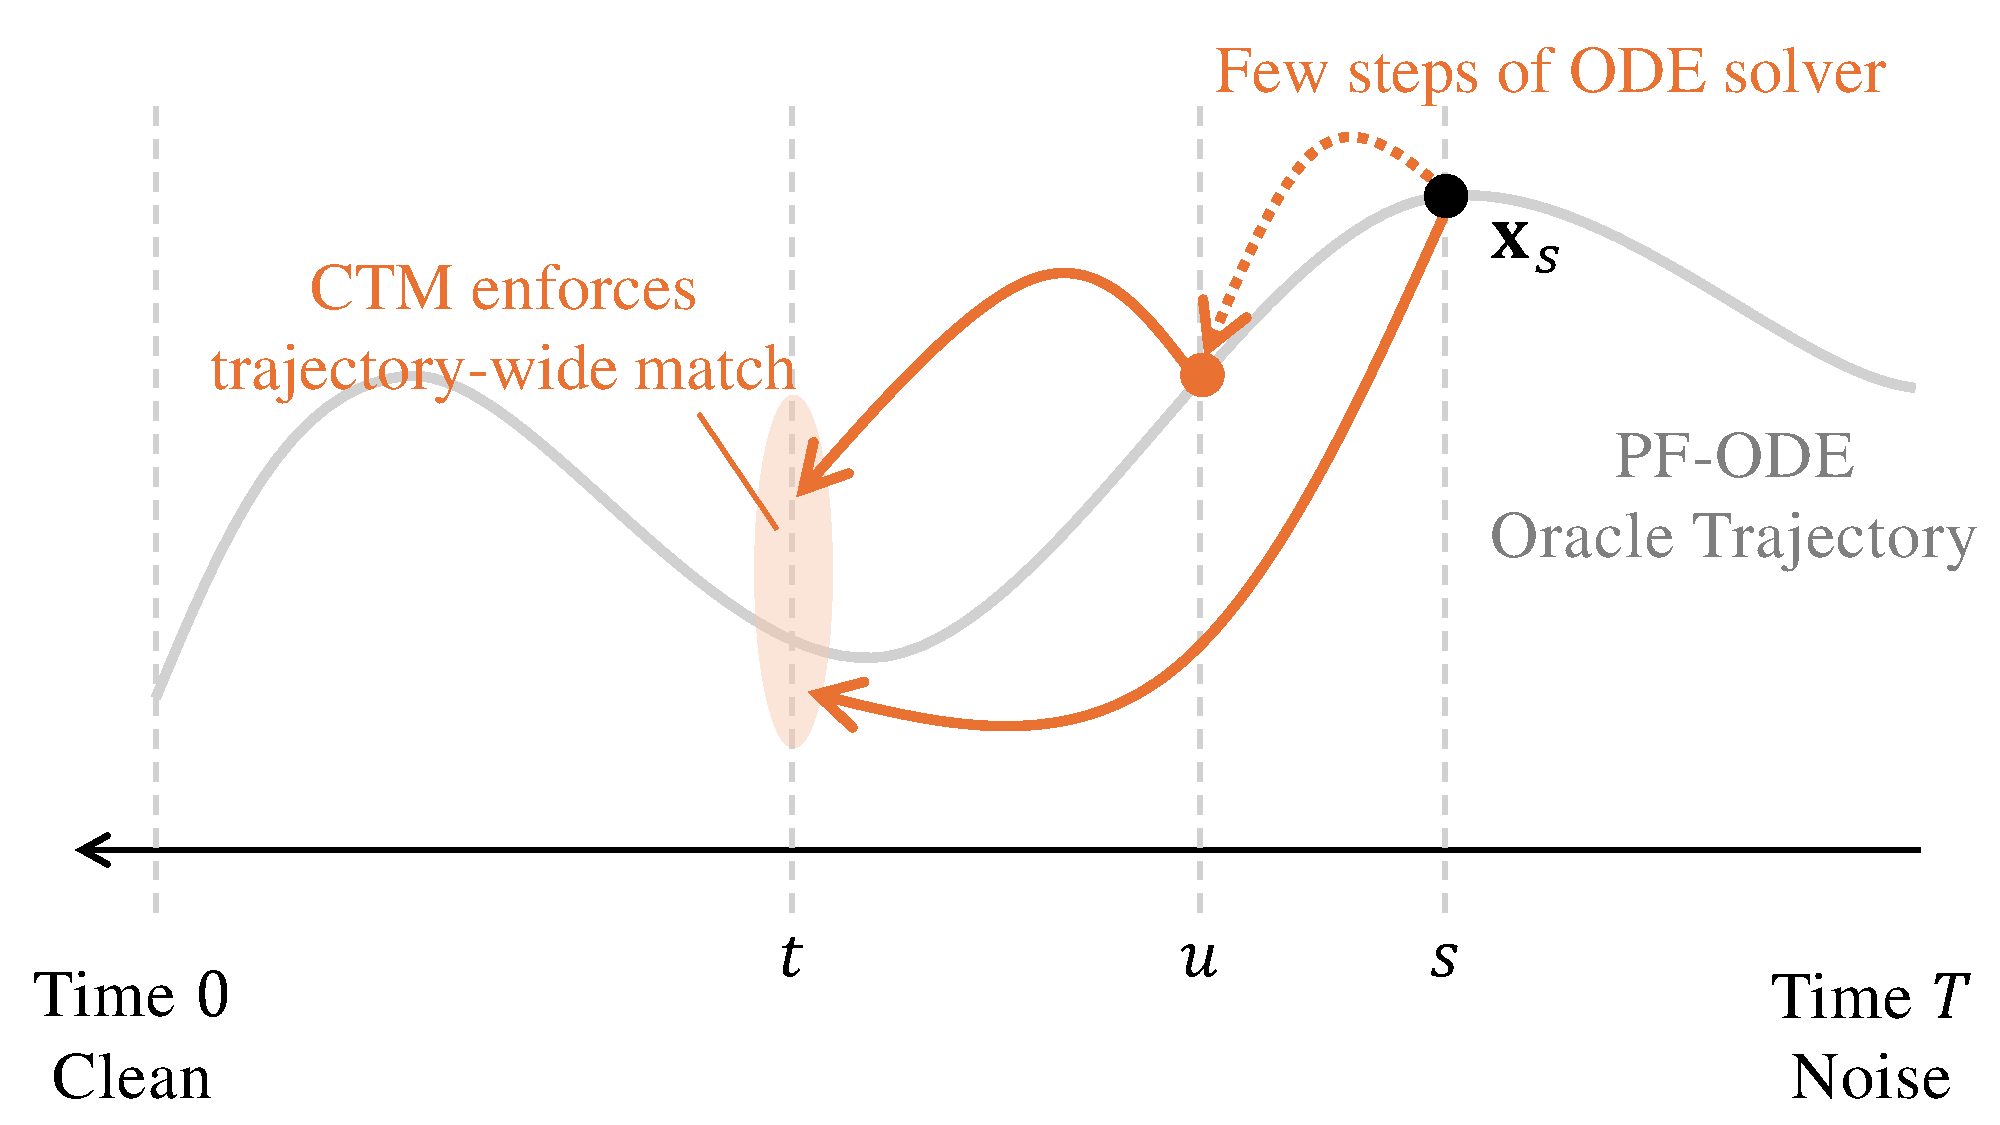
\includegraphics[width=0.9\linewidth]{Images/PartD/ctm-target.pdf}
    \caption{\textbfs{CTM 半群性质的示意图。} 对任意 $s \ge u \ge t$，CTM 强制
    $\rmG_{\btheta}(\rvx_s, s,  t)
\approx
\rmG_{\btheta^-} \big(\mathtt{Solver}_{s\to u}(\rvx_s), u ,  t\big)$，
即一段短求解器段 $s \to u$ 后接一个到 $t$ 的 CTM “跳转”，匹配直接的 CTM 映射 $s\to t$。求解器可以是预训练扩散模型或 CTM 的自诱导教师。\figcredit{改编自 \citet{kim2023consistency}。}}
    \label{fig:ill_models}
\end{figure}

\subsection{CTM 中的辅助损失}\label{subsec:ctm-auxiliary}

（自）蒸馏可能表现不如教师，因为它仅对教师生成的目标进行优化，缺乏来自真实数据的直接监督。相比之下，CTM 能自然地纳入数据驱动的正则化项，例如通过在目标中增加去噪得分匹配和对抗（GAN）项~\citep{goodfellow2014generative}，以更好地学习流映射。

\paragraph{扩散损失的自然整合。}
扩散模型损失（更准确地说是条件流匹配损失；见\Cref{eq:fm-cfm}）自然地整合进 CTM，并提供一个固定的回归目标，便于流映射模型的学习。为看清这一点，注意我们有
\[
\rvv^*(\rvx_s, s)
= \frac{\rvx_s - \rvg^*(\rvx_s, s, s)}{s},
\qquad
\rvg^*(\rvx_s, s, s) \approx \rvg_{\btheta}(\rvx_s, s, s).
\]
这自然通过 $\rvg_{\btheta}$ 诱导出一个速度参数化：
\[
\rvv_{\btheta}(\rvx_s, s)
:= \frac{1}{s}\bigl(\rvx_s - \rvg_{\btheta}(\rvx_s, s, s)\bigr).
\]
使用线性高斯路径
\[
\rvx_s = \alpha_s \rvx_0 + \sigma_s \beps,
\qquad
\rvx_0 \sim p_{\mathrm{data}},
\beps \sim \mathcal N(0, \mathbf I),
\]
扩散模型损失可以写为
\begin{align}\label{eq:ctm-dsm}
\mathcal L_{\mathrm{DM}}(\btheta)
&:= 
\E_{\rvx_0, \beps, s}
\Bigl[
w(s)
\bigl\|
 \rvv_{\btheta}(\rvx_s, s) - \left(\alpha_s' \rvx_0 + \sigma_s' \beps\right)
\bigr\|_2^2
\Bigr].
\end{align}



$\mathcal L_{\mathrm{DM}}$ 在 $t$ 接近 $s$ 时通过显式监督轨迹上的小跳来提高精度。在该体系下，\Cref{eq:ctm_para_1}中的因子 $1-\tfrac{t}{s}$
接近零，可能削弱梯度并减缓
学习；$\mathcal L_{\mathrm{DM}}$ 提供更强的局部信号并稳定训练。

从概念上讲，\Cref{eq:ctm-consist-distill,eq:ctm-consist-scratch}强制
轨迹匹配（零阶），而\Cref{eq:ctm-dsm}强制
斜率匹配（一阶）。

\paragraph{(可选) GAN 损失。}
虽然一致性和扩散模型损失提供了强的回归信号，但它们可能产生
过度平滑的输出。CTM 因此可选地加入一个对抗项以
通过将生成器
分布与数据分布对齐来鼓励更锐利、更真实的样本。用一个判别器
$D_{\bm{\zeta}}$ 区分真实 $\rvx_{0}\sim p_{\mathrm{data}}$ 和
生成的 $\rvx_{\mathrm{est}}(\rvx_{s},s,t)$，目标为
\begin{align*}
&\mathcal{L}_{\mathrm{GAN}}(\bm{\theta}, \bm{\zeta}) := \\ &\mathbb{E}_{\mathbf{x}_0} \big[\log D_{\bm{\zeta}}(\mathbf{x}_0)\big] + \mathbb{E}_{s \in [0, T]} \mathbb{E}_{t \in [0, s]} \mathbb{E}_{\mathbf{x}_0} \mathbb{E}_{\mathbf{x}_s \vert \mathbf{x}_0} \big[\log (1 - D_{\bm{\zeta}}( \mathbf{x}_{\mathrm{est}}(\mathbf{x}_s, s, t)))\big], \end{align*}
其中 $D_{\bm{\zeta}}$ 被最大化，$\rmG_{\bm{\theta}}$ 被最小化。
直观上，判别器充当一个自适应的感知距离，
鼓励真实的细节。理论上，GAN 项驱动
$p_{\mathrm{data}}$ 与 $\rmG_{\bm{\theta}}$ 所诱导模型分布之间的
分布匹配（Jensen-Shannon 散度）~\citep{goodfellow2014generative}，
这可能使保真度超越教师。

\paragraph{CTM 总目标。}
总之，CTM 将（自）蒸馏、扩散和 GAN 损失统一到单一训练框架中：
\begin{mdframed}
    \begin{align*}
\mathcal{L}_{\mathrm{CTM}}(\bm{\theta},\bm{\zeta})
:=  \mathcal{L}_{\mathrm{consist}}(\bm{\theta};  \bm{\phi}^\times/\bm{\theta}^-)
+ \lambda_{\mathrm{DM}} \mathcal{L}_{\mathrm{DM}}(\bm{\theta})
+ \lambda_{\mathrm{GAN}} \mathcal{L}_{\mathrm{GAN}}(\bm{\theta},\bm{\zeta}),
\end{align*}
\end{mdframed}
其中教师或者是外部预训练模型 $\bm{\phi}^\times$，或者是
自诱导教师 $\bm{\theta}^-$。回归式分量
$\mathcal{L}_{\mathrm{consist}}$ 和 $\mathcal{L}_{\mathrm{DM}}$ 充当强
正则化项，而可选的 GAN 项在不
牺牲稳定性的前提下改善细尺度细节~\citep{kim2024pagoda}。


\subsection{使用 CTM 进行灵活采样}
CTM 学习任意 $s>t$ 的一般流映射 $\bPsi_{s\to t}$，这意味着它支持
任意时刻到任意时刻的转移。这一性质使灵活的采样策略成为可能。
例如，CTM 提出 \emph{$\gamma$ 采样}，其中超参数 $\gamma$
控制生成过程中的随机性。
此外，CTM 可以复用为扩散模型开发的标准推理技术，
例如基于 ODE 的求解器和精确似然计算。

在下文中，我们固定一个离散时间网格用于采样 $T=\tau_0 > \tau_1 > \tau_2 > \cdots > \tau_{M}=0$。

\begin{algorithm}[H]
    \centering
    \caption{CTM 的 $\gamma$-采样}\label{alg:gamma}
    \begin{algorithmic}[1]
    \Require 训练好的 CTM $\mathbf{G}_{\bm{\theta}^\times}$，$\gamma\in[0,1]$，$T=\tau_0>\tau_1 > \tau_2 > \cdots > \tau_{M}=0$。
    \State 从 $\mathbf{x}_{\tau_{0}}\sim p_{\mathrm{prior}}=\mathcal{N}(\bm{0}, T^2\rmI)$ 开始
        \For{$n=0$ 到 $M-1$}
        \State $\tilde{\tau}_{n+1}\leftarrow \sqrt{1-\gamma^{2}}\tau_{n+1}$
        \State 去噪 $\mathbf{x}_{\tilde{\tau}_{n+1}}\leftarrow \mathbf{G}_{\bm{\theta}^\times}(\mathbf{x}_{\tau_{n}},\tau_{n},\tilde{\tau}_{n+1})$
        \State 加噪 $\mathbf{x}_{\tau_{n+1}}\leftarrow\mathbf{x}_{\tilde{\tau}_{n+1}}+\gamma \tau_{n+1}\bm{\epsilon}$，其中 $\bm{\epsilon}\sim\mathcal{N}(\bm{0}, \rmI)$
        \EndFor
        \Ensure  $\mathbf{x}_{\tau_{M}}$
    \end{algorithmic}
\end{algorithm}

\paragraph{$\gamma$-采样方法论。}
CTM 的 $\gamma$-采样引入了一个统一的采样器家族，它自然地产生于学习一般流映射模型。
它涵盖了先前的方法，例如 CM 的多步采样（见\Cref{alg:cm_sampling}）
以及时间步进式采样，后者在概念上类似于 ODE 求解器。
参数 $\gamma$ 直接控制生成过程中语义变化的程度，
使 $\gamma$ 采样成为针对多样下游应用的灵活且任务感知的策略。





\begin{figure}[t]
    \centering
    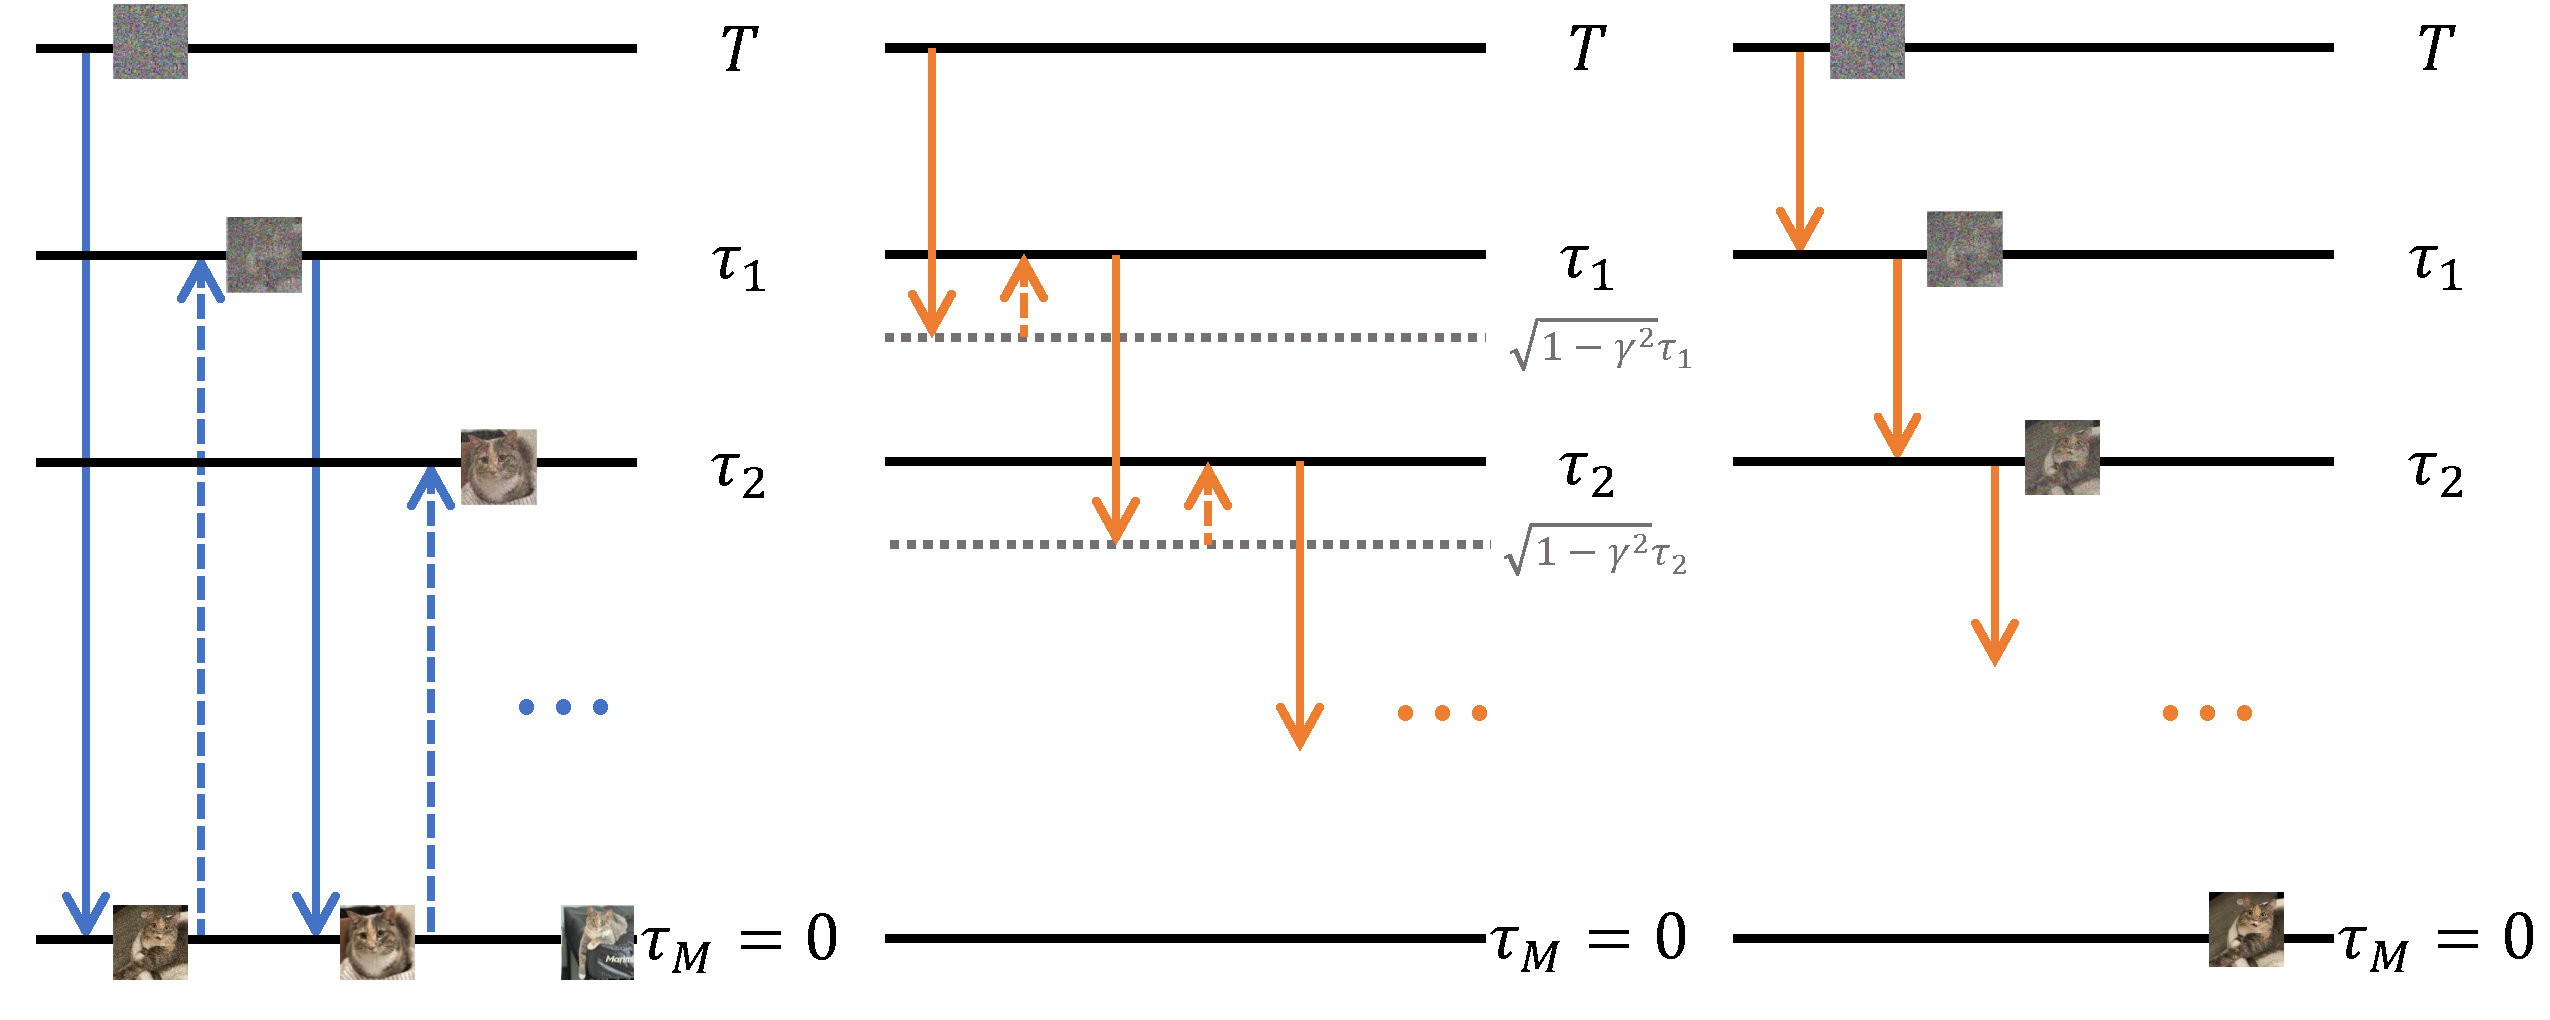
\includegraphics[width=\linewidth]{Images/PartD/ctm_gamma.pdf}
    \caption{\textbfs{不同 $\gamma$ 值下 $\gamma$-采样的示意图。} 该过程在网络求值去噪与反向加噪之间交替，   $(\tau_{n}\xrightarrow{\text{去噪}} \sqrt{1-\gamma^{2}}\tau_{n+1}\xrightarrow{\text{加噪}} \tau_{n+1})_{n=0}^{M-1}$。
最左边的面板展示了 $\gamma=1$，对应完全随机的情形。
最右边的面板展示了 $\gamma=0$，对应完全确定的情形。
中间的面板描绘了中间值 $\gamma\in(0,1)$，在两个极端之间插值。
\figcredit{改编自 \citet{kim2023consistency}。}}
    \label{fig:gamma_sampling}
\end{figure}


\begin{itemize}
\item \Cref{fig:gamma_sampling}-（左）：当 $\gamma=1$ 时，它恰好与 CM 中引入的多步采样（即特殊流映射 $\bPsi_{s\to 0}$）重合，是完全随机的，并在步数变化时产生语义变化。

\item \Cref{fig:gamma_sampling}-（右）：当 $\gamma=0$ 时，它退化为完全确定时间步进，估计 PF-ODE 的解轨迹。$\gamma=0$ 的 $\gamma$ 采样与传统基于时间步进 ODE 的采样之间的一个关键区别是，CTM 避免了数值求解器的离散化误差。

\item \Cref{fig:gamma_sampling}-（中）：当 $0 < \gamma < 1$ 时，$\gamma$-采样通过允许在采样过程中注入可控量的随机性，在两个极端之间插值。
\end{itemize}
我们强调，能够实现 $\gamma \in (0,1]$ 的采样器只有在模型学习一般流映射 $\bPsi_{s\to t}$ 时才可能。

\paragraph{$\gamma$-采样分析。} CTM 经验观察到，一旦步数 $M \geq 4$，CM 的多步采样质量就会下降。
为解释这一现象，CTM 分析了潜在原因：当 $\gamma \neq 0$ 时，每次神经“跳转”都会引入小的失配，而这些失配随着模型迭代地将状态映射向时刻零而累积。这种误差累积解释了为何长的多步运行可能表现不佳。我们在如下命题中将这一思想形式化。

\proppp{(非正式) 两步 $\gamma$-采样}{ctm-gamma}{
\label{th:sampling_agg_error_2_steps}
令 $\tau\in(0,T)$，$\gamma \in [0,1]$。设 $p_{\bm{\theta}^{*},2}$ 为由最优 CTM 的 $\gamma$-采样器得到的密度，遵循转移序列 $
    T\rightarrow\sqrt{1-\gamma^2}\tau\rightarrow \tau \rightarrow 0
$，从 $p_{\mathrm{prior}}$ 出发。则
 \begin{align*}
    \mathcal D_{\mathrm{TV}}\big( p_{\mathrm{data}}, p_{\bm{\theta}^{*},2} \big)         = \mathcal{O}\left(\sqrt{T-\sqrt{1-\gamma^2}\tau+ \tau}  \right).
 \end{align*}
 这里，$\mathcal{D}_{\mathrm{TV}}$ 表示分布之间的全变差距离（见\Cref{eq:f-div}）。
}{
关于采样步数为 $M$ 的一般情形，我们请读者参考 \citet{kim2023consistency} 的定理 8。 }
从上述定理得到的洞见可总结如下：
\begin{itemize}
    \item \textbfs{当} $\gamma = 1$（对应 CM 的多步采样）\textbfs{时：}该方法在每步 $n$ 进行从 $\tau_n$ 到 $0$ 的迭代长程转移。这导致量级为
    \begin{align*}
        \mathcal{O}\left(\sqrt{T + \tau_1 + \cdots + \tau_M}\right).
    \end{align*}
    的误差累积。

    \item \textbfs{当} $\gamma = 0$（对应 CTM 的确定性多步采样）\textbfs{时：}这种转移之间的时间重叠被消除。这避免了误差累积并给出更紧的界 $\mathcal{O}(\sqrt{T})$。经验上，$\gamma = 0$ 的 CTM 在采样速度和样本质量之间提供了有利的折中：增加采样步数可提升生成质量而不会引入不稳定。
\end{itemize}


\paragraph{CTM 支持扩散推理。} 由于 CTM 通过 $\rvg_{\bm{\theta}}$ 直接学习得分函数（或去噪器），
得益于其在\Cref{eq:ctm_para_1}中的参数化，它与最初为
扩散模型开发的推理技术兼容。例如，可以使用 $\rvg_{\bm{\theta}}(\cdot, s, s)$
计算精确似然
（\Cref{subsec:sde-sample}）或应用诸如 DDIM 或 DPM 的高级求解器（\Cref{ch:solvers}）
进行生成。




\newpage

\section{\texorpdfstring{一般流映射：均值流}{General Flow Map: Mean Flow}}\label{sec:MF}


正如扩散模型允许许多等价的参数化和训练目标，一般流映射 $\bPsi_{s\to t}$ 也可以通过多种合理的方式来学习。
在本节中，我们介绍\emph{均值流}（MF）~\citep{geng2025mean}，它是通用流映射族 $\bPsi_{s\to t}$ 的一个较晚的代表，展示了一种不同但有原则的视角，说明这类映射如何被有效地学习。



\subsection{均值流的建模与训练}

与建立在 EDM 框架上的 CM 和 CTM 不同，MF 基于
流匹配公式（对 $t\in[0,1]$，$\alpha_t = 1-t$，$\sigma_t  = t$）。
MF 不是直接对流映射进行参数化，而是学习区间 $[t,s]$（$t<s$）上的\emph{平均漂移}：
\[
\rvh_{\btheta}(\rvx_s, s, t)  \approx
\rvh^*(\rvx_s, s, t) := \frac{1}{t-s}\int_s^t \rvv^*(\rvx_u,u) \diff u.
\]
相应的 oracle 损失为
\begin{align}\label{eq:mf-oracle}
\mathbb{E}_{t<s} \mathbb{E}_{\rvx_s\sim p_s}\Big[w(s)
\|\rvh_{\btheta}(\rvx_s,s,t) - \rvh^*(\rvx_s,s,t)\|_2^2\Big].
\end{align}
特别地，当 $s \to t$ 时，损失函数退化为流匹配损失：
\begin{align}\label{eq:mf-to-fm}
    \mathbb{E}_{t} \mathbb{E}_{\rvx_t\sim p_t}\Big[w(t)
\|\rvh_{\btheta}(\rvx_t,t,t) - \rvv^*(\rvx_t,t)\|_2^2\Big],
\end{align}
学习的是瞬时速度。
我们在后文\Cref{subsec:equivalence-ctm-mf}中将看到，MF 与
\Cref{eq:general-cm-loss:rep}中的一般目标保持一致，
但从一个不同（然而等价）的视角来处理它。
由于 oracle 回归目标 $\rvh^*(\rvx_s,s,t)$ 一般没有闭式，MF 通过对恒等式
\[
(t-s)\,\rvh^*(\rvx_s,s,t) = \int_s^t \rvv^*(\rvx_u,u)\,\diff u
\]
关于 $s$ 求导所得的恒等式来构造一个代理。这给出\emph{MF 恒等式}：
\begin{align}\label{eq:mf-identity}
\begin{aligned}
    \rvh^*(\rvx_s,s,t)
&= \rvv^*(\rvx_s,s) - (s-t) \tfrac{\diff}{\diff s}\rvh^*(\rvx_s,s,t) \\
&= \rvv^*(\rvx_s,s) - (s-t)\Big[(\partial_{\rvx}\rvh^*)(\rvx_s,s,t) \rvv^*(\rvx_s,s) 
+ \partial_s \rvh^*(\rvx_s,s,t)\Big],
\end{aligned}
\end{align}
其中第二行应用链式法则以及
\[
\frac{\diff}{\diff s}\rvx_s = \rvv^*(\rvx_s,s).
\]

受此恒等式启发，MF 用一个停梯度代理替代不可达的 oracle，得到实用的训练目标
\begin{mdframed}
\begin{align}\label{eq:mf-practice}
    \mathcal{L}_{\mathrm{MF}}(\btheta)
:= \mathbb{E}_{t<s} \mathbb{E}_{\rvx_s\sim p_s}\Big[w(s)\,
\|\rvh_{\btheta}(\rvx_s,s,t) - \rvh_{\btheta^-}^{\mathrm{tgt}}(\rvx_s,s,t)\|_2^2\Big],
\end{align}
\end{mdframed}
其中回归目标定义为
\begin{align*}
    \rvh_{\btheta^-}^{\mathrm{tgt}}&(\rvx_s,s,t)
:= \\ &\rvv^*(\rvx_s,s) - (s-t)\Big[\underbrace{(\partial_{\rvx}\rvh_{\btheta^-})(\rvx_s,s,t) \rvv^*(\rvx_s,s)
+ \partial_s \rvh_{\btheta^-}(\rvx_s,s,t)}_{\mathrm{JVP}}\Big].
\end{align*}

实践中，oracle 速度 $\rvv^*$ 不能以闭式计算，
必须被近似。有两种常见策略：依赖
预训练扩散模型（\emph{蒸馏}）或从数据中构造直接
估计器（\emph{从零开始训练}）。无论作何选择，最终都需要计算目标网络
$\rvh_{\btheta^-}$ 的一个\emph{雅可比-向量积}（JVP）：
\[
\left[\partial_\rvx \rvh_{\btheta^-}, \partial_s \rvh_{\btheta^-}, \partial_t \rvh_{\btheta^-}\right]^\top \cdot \left[\rvv^*, 1, 0\right]
\]


\paragraph{蒸馏。}
使用具有流匹配骨干的预训练扩散模型，
$\rvv_{\bphi^\times} \approx \rvv^*$。

\paragraph{从零开始训练。}
使用单点条件速度 $\alpha_s'\rvx_0 + \sigma_s'\beps$，
由前向加噪 $\rvx_s=\alpha_s\rvx_0+\sigma_s\beps$ 得到，其中
$\beps\sim\mathcal N(\bm{0},\rmI)$。这给出了在配对 $(\rvx_0,\beps)$ 处求值时层级 $s$ 瞬时漂移的无偏单样本估计。

% We emphasize that MF’s strength lies in its strong performance in the training-from-scratch setting. It requires no pre-trained model for initialization or guidance during training, and it does not rely on additional regularizers (such as a GAN loss). In this sense, MF serves as a fully standalone generative model.

\subsection{均值流的采样}
一旦均值流 $\rvh_{\btheta^\times}$ 训练完成，它自然地恢复出流映射的一个代理。对任意起点 $\rvx_s$，从 $s$ 到 $t$ 的映射（近似）为
\[
\bPsi_{s\to t}(\rvx_s) = \rvx_s + (t-s)\,\rvh^*(\rvx_s,s,t)
  \approx   \rvx_s + (t-s)\,\rvh_{\btheta^\times}(\rvx_s,s,t).
\]

这使得单步和多步采样都成为可能。例如，抽取
$\rvx_T\sim p_{\mathrm{prior}}$，干净样本的单步生成为
\[
\rvx_0  \leftarrow  \rvx_T + T\,\rvh_{\btheta^\times}(\rvx_T,T,0).
\]

或者，可以通过准备一个时间网格并按序施加映射
来进行多步生成，采用与
CTM 相同的时间步进方式。由于 MF 学习的是一般流映射，它也支持
CTM 中的 $\gamma$-采样，其中可控超参数 $\gamma$ 向采样过程注入随机性。



\subsection{CTM 与 MF 之间的关系}\label{subsec:equivalence-ctm-mf}
乍看之下，CTM 与 MF 似乎并不相关。
事实上，两者都只是同一 oracle 流映射 $\bPsi_{s\to t}$ 的不同参数化，它们的训练损失（CTM 的一致性损失与\Cref{eq:mf-oracle}）仅在时间加权上有所不同~\citep{hu2025cmt}。

\paragraph{参数化之间的关系。}
两种方法都在同一一般框架下运作，但以不同的方式表示所学函数。
流映射可以等价写为
\begin{align*}
\bPsi_{s\to t}(\rvx_s)
& = \rvx_s + \int_s^t \rvv^*(\rvx_u, u)\diff u \\
&= \frac{t}{s}\rvx_s
   + \frac{s-t}{s}\underbrace{\Bigg[\rvx_s + \frac{s}{s-t}\int_s^t \rvv^*(\rvx_u,u)\,\diff u\Bigg]}_{\approx\,\rvg_\btheta} \\
&= \rvx_s + (t-s)\underbrace{\Bigg[\frac{1}{t-s}\int_s^t \rvv^*(\rvx_u,u)\,\diff u\Bigg]}_{\approx\,\rvh_\btheta}.
\end{align*}
这里，第一个是流映射的定义，第二个形式通过 $\rvg_\btheta$ 突出 CTM 参数化（见\Cref{eq:ctm-g-oracle,eq:ctm_para_1}），最后一个通过 $\rvh_\btheta$ 突出 MF 参数化。


\paragraph{训练损失之间的关系。} 给定上述用 CTM 参数化对 oracle 流映射 $\bPsi_{s\to t}$ 的重新解释
\[
\rvg_\btheta(\rvx_s,s,t) \approx \rvg^*(\rvx_s,s,t):=\rvx_s + \frac{s}{s-t}\int_s^t \rvv^*(\rvx_u,u) \diff u
\]
 和 MF 参数化
\[
\rvh_\btheta(\rvx_s,s,t) \approx \rvh^*(\rvx_s,s,t):=\frac{1}{t-s}\int_s^t \rvv^*(\rvx_u,u) \diff u,
\]
我们现在说明 CTM 和 MF 的训练损失实际上是等价的。


考虑关系
\[
\rvg_\btheta(\rvx_s,s,t) := \rvx_s - s \rvh_\btheta(\rvx_s,s,t),
\]
并以 $d(\rvx,\rvy):=\|\rvx-\rvy\|^2$ 为例。代入\Cref{eq:general-cm-loss:rep}并将 $\rmG_\btheta$ 视为 CTM 的流映射参数化（\Cref{eq:ctm_para_1}）得到
\begin{align} &~d\big(\rmG_\btheta(\rvx_s,s,t), \bPsi_{s\to t}(\rvx_s)\big) \notag \\ = &~\norm{\rmG_\btheta(\rvx_s,s,t) - \bPsi_{s\to t}(\rvx_s)}^2 \notag \\ = &~\norm{\left(\frac{t}{s}\rvx_s + \frac{s-t}{s} \rvg_\btheta(\rvx_s,s,t)\right)-\left(\frac{t}{s}\rvx_s + \frac{s-t}{s}\Big[\rvx_s + \frac{s}{s-t}\int_s^t \rvv^*(\rvx_u,u) \diff u\Big]\right)}^2 \notag \\ = &~\left(\frac{s-t}{s}\right)^2\norm{\rvg_\btheta(\rvx_s,s,t)-\left(\rvx_s + \frac{s}{s-t}\int_s^t \rvv^*(\rvx_u,u) \diff u\right)}^2 \label{eq:g-para} \\ = &~\left(\frac{s-t}{s}\right)^2\norm{\left(\rvx_s - s \rvh_\btheta(\rvx_s,s,t)\right)-\left(\rvx_s + \frac{s}{s-t}\int_s^t \rvv^*(\rvx_u,u) \diff u\right)}^2 \notag \\ = &~\left(\frac{s-t}{s}\right)^2\norm{\left(\rvx_s - s \rvh_\btheta(\rvx_s,s,t)\right)-\left(\rvx_s + \frac{s}{s-t}\int_s^t \rvv^*(\rvx_u,u) \diff u\right)}^2 \notag \\ = &~\left(s-t\right)^2\norm{ \rvh_\btheta(\rvx_s,s,t)- \left(\frac{1}{t-s}\int_s^t \rvv^*(\rvx_u,u)\diff u \right)}^2 \label{eq:h-para} \end{align}
 因此，
\begin{align*}
\frac{1}{s^2} \Bigg\|\rvg_\btheta(\rvx_s,s,t)-\rvg^*(\rvx_s,s,t) \Bigg\|^2 = \Bigg\|\rvh_\btheta(\rvx_s,s,t)-\rvh^*(\rvx_s,s,t) \Bigg\|^2.
\end{align*}
撇开用于学习流映射的具体算法不谈，CTM 和 MF 的损失具有相同的数学形式，仅相差一个加权函数。此外，在两种情形中令 $t=0$ 都恢复 CM 的设定（$\bPsi_{s\to 0}$），其中
每个状态直接映射到干净数据。

\paragraph{实践中的辅助损失。}
在 CTM 中，训练是用\Cref{eq:ctm-consist-scratch}中的一致性损失与\Cref{eq:ctm-dsm}中其自定义的扩散模型损失联合进行的。MF 采用了类似的策略。如\Cref{eq:mf-to-fm}所示，当 $s \to t$ 时，MF 损失退化为标准流匹配目标。实践中，MF 控制 $s \neq t$ 对与 $s = t$ 对之间的比例；因此，整体优化变成\Cref{eq:mf-practice}中 MF 目标与\Cref{eq:mf-to-fm}中流匹配目标的混合。

两种参数化都能够实现从扩散模型训练（以固定回归目标学习瞬时速度）到流映射学习（采用停梯度伪回归目标）的平滑过渡。


\paragraph{CTM 和 MF 参数化都支持灵活推理。}
CTM（$\rmG_\btheta(\rvx_s,s,t)$）和 MF（$\rvh_\btheta(\rvx_s,s,t)$）都旨在近似底层流映射 $\bPsi_{s\to t}$：
\[
\rmG_\btheta(\rvx_s,s,t)\approx\bPsi_{s\to t},\quad  \text{且}
\quad
\rvx_s+(t-s)\rvh_\btheta(\rvx_s,s,t)\approx\bPsi_{s\to t}.
\]
由于两个模型都学习任意两个时间步之间的显式映射，它们自然支持 CTM 的 $\gamma$-采样，并与最初为扩散模型开发的推理技术兼容，例如引导（\Cref{ch:guidance}）、精确似然计算（\Cref{eq:score-sde-likelihood}）以及使用高阶求解器的加速采样（\Cref{ch:solvers}）。
这种兼容性源于它们的参数化在无穷小极限 $t\to s$ 下恢复瞬时扩散漂移：
\[
\rvg^*(\rvx_s,s,s)=\rvx_s-\rvv^*(\rvx_s,s),
\quad  \text{且}
\quad
\rvh^*(\rvx_s,s,s)=\rvv^*(\rvx_s,s).
\]
特殊化流映射公式 $\bPsi_{s\to0}$（如 CM 系列）不具备这一性质。因此，CTM 和 MF 都可视为灵活、一般的流映射公式，将基于扩散的推理推广到直接的时间到时间映射。




\paragraph{结论。}
% This equivalence between CTM and MF is similar to the situation in diffusion models (\Cref{sec:equivalent-parametrizations}), where different parameterizations ultimately describe the same underlying oracle target. In principle, these formulations are mathematically identical. In practice, however, their behavior can differ because of factors such as loss weighting, network design, or optimization dynamics, which may cause one approach to perform better than another under specific conditions.


CTM 与 MF 之间的关系类似于扩散模型中的情形（\Cref{sec:equivalent-parametrizations}），不同的参数化最终描述的是同一底层 oracle 目标。就学习对象而言，这些公式在数学上是等价的；在损失目标层面，它们可视为等价。

尽管 CTM 和 MF 存在这种关联，它们在学习目标的方式上，无论在概念上还是算法上都有所不同。CTM 目标以“积分”形式定义，因为它直接作用于流映射。而 MF 目标以“微分”形式定义，因为它依赖于流映射的有限差分。由于积分形式的目标不可直接处理，CTM 必须在训练过程中求解一个 ODE。相比之下，MF 利用 MF 恒等式（见\Cref{eq:mf-identity}）构造一个可处理的微分形式目标。这种关系类似于基于能量与基于得分方法之间的关系：前者学习概率密度本身（积分形式），后者匹配该密度的梯度（微分形式）。实践中，由于损失加权、网络架构和优化动力学等因素，CTM 和 MF 可能表现不同，这些因素可能使一种方法在某些条件下优于另一种。

这一视角表明 CTM 和 MF 并非唯一可行的公式。流映射的其他参数化也可能实现高效、稳定的训练，潜在地带来新的独立生成模型。探索这些替代方案可能会进一步丰富扩散模型及其流映射扩展的版图，推动少步生成的边界。

\newpage

\section{结语}\label{sec:ch11_cr}

本章为我们的探索画上了完整的闭环：从缓慢的迭代
扩散采样器到快速的少步生成器（从零开始学习）。本章各方法背后的共同对象是
\Cref{eq:general-cm-loss:rep}中引入的 oracle 流映射：
\[
\bPsi_{s\to t}(\rvx_s)
=
\rvx_s+\int_s^t \rvv^*(\rvx_\tau,\tau)\,\diff \tau.
\]
学习该映射用一次或少数几次学习到的跳转
取代了大量小的数值更新。

至此，跳出单个算法来看是有益的。
知识蒸馏（\Cref{sec:distillation-prologue}）、渐进式蒸馏（\Cref{sec:PD}）、CM（\Cref{sec:discrete-cm}）、CTM
（\Cref{sec:CTM}）和 MF（\Cref{sec:MF}）通过不同的
训练构造引入，但它们都显式或隐式地利用了相同的
ODE 解映射结构。\citet{boffi2024flow} 的流映射框架
为精确刻画这一共同结构提供了一种后来的系统性语言\footnote{我们在本部分的表述和插图也受到
\citet{dieleman2026flowmaps} 清晰论述的启发。}。在这一视角下，同一 oracle 流映射可通过三种
数学上等价的视角来解读：\emph{半群视角}、
\emph{拉格朗日视角}和\emph{欧拉视角}。这些视角提供了一种
有原则且经典的方式来描述 ODE 流下的粒子输运，
在此作为上述方法的一种组织透镜，
同时保留每种方法独特的算法贡献。

\paragraph{半群视角：拆分行程。}
如\Cref{eq:semi-group}中所引入，有限步恒等式为
\[
\bPsi_{u\to t}\big(\bPsi_{s\to u}(\rvx_s)\big)
=
\bPsi_{s\to t}(\rvx_s).
\]
如\Cref{fig:semigroup}所示，其直觉与沿固定路线行进相同：从 $s$ 到
$u$ 再从 $u$ 到 $t$，与直接从
$s$ 到 $t$ 到达同一点。在此视角下，KD 是退化的全程跳转情形 $\bPsi_{T\to0}$，PD
将两个相邻教师步压缩为一个学生步，CM 学习
特殊的任意时刻到干净样本的映射 $\bPsi_{s\to0}$，而 CTM 将同样的
复合原则推广到一般映射 $\bPsi_{s\to t}$。

\begin{figure}[t]
    \centering

    \begin{subfigure}[t]{0.485\textwidth}
        \centering
        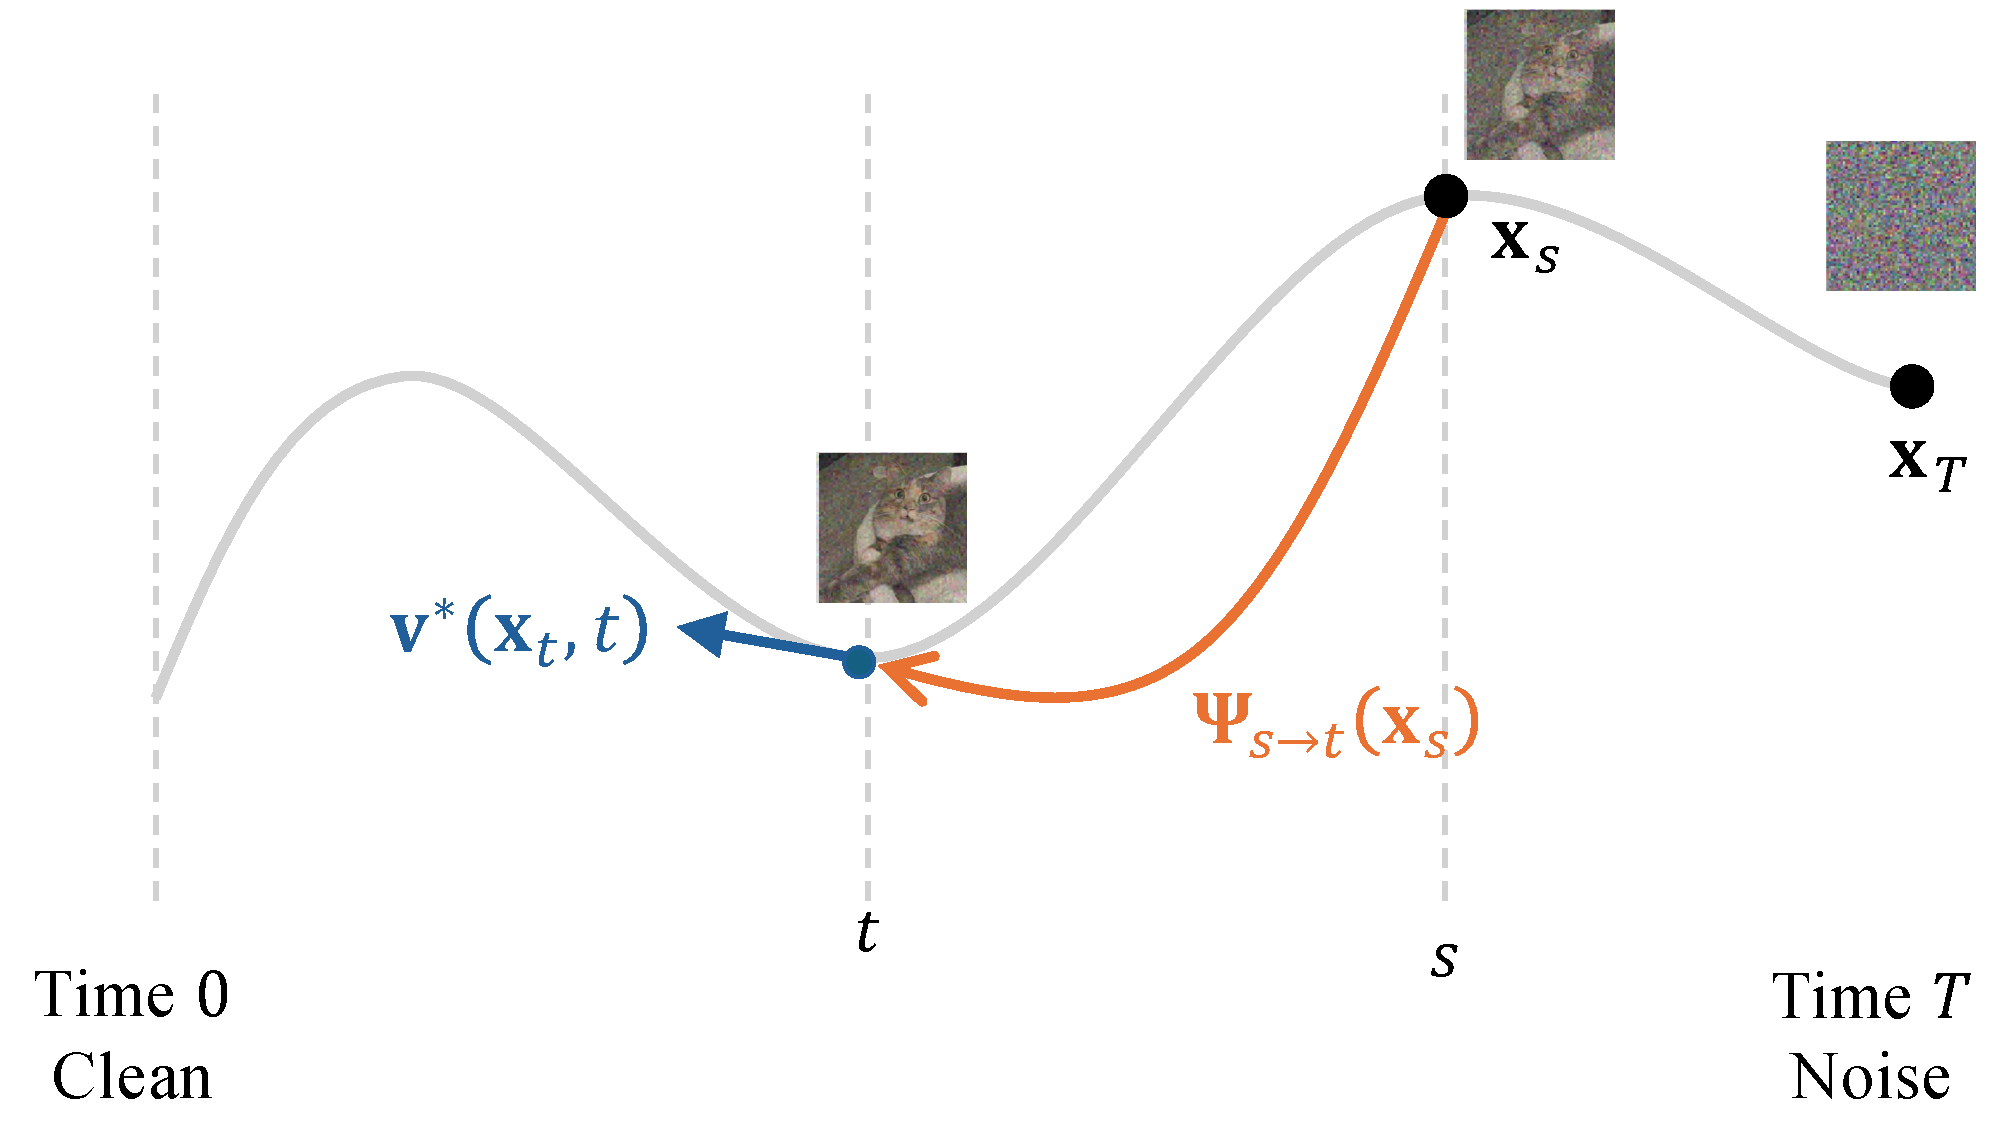
\includegraphics[width=\linewidth]{Images/PartD/lagrangian-1.pdf}
        \caption{基准目标时刻 $t$。}
        \label{fig:lagrangian-base}
    \end{subfigure}
    \hfill
    \begin{subfigure}[t]{0.485\textwidth}
        \centering
        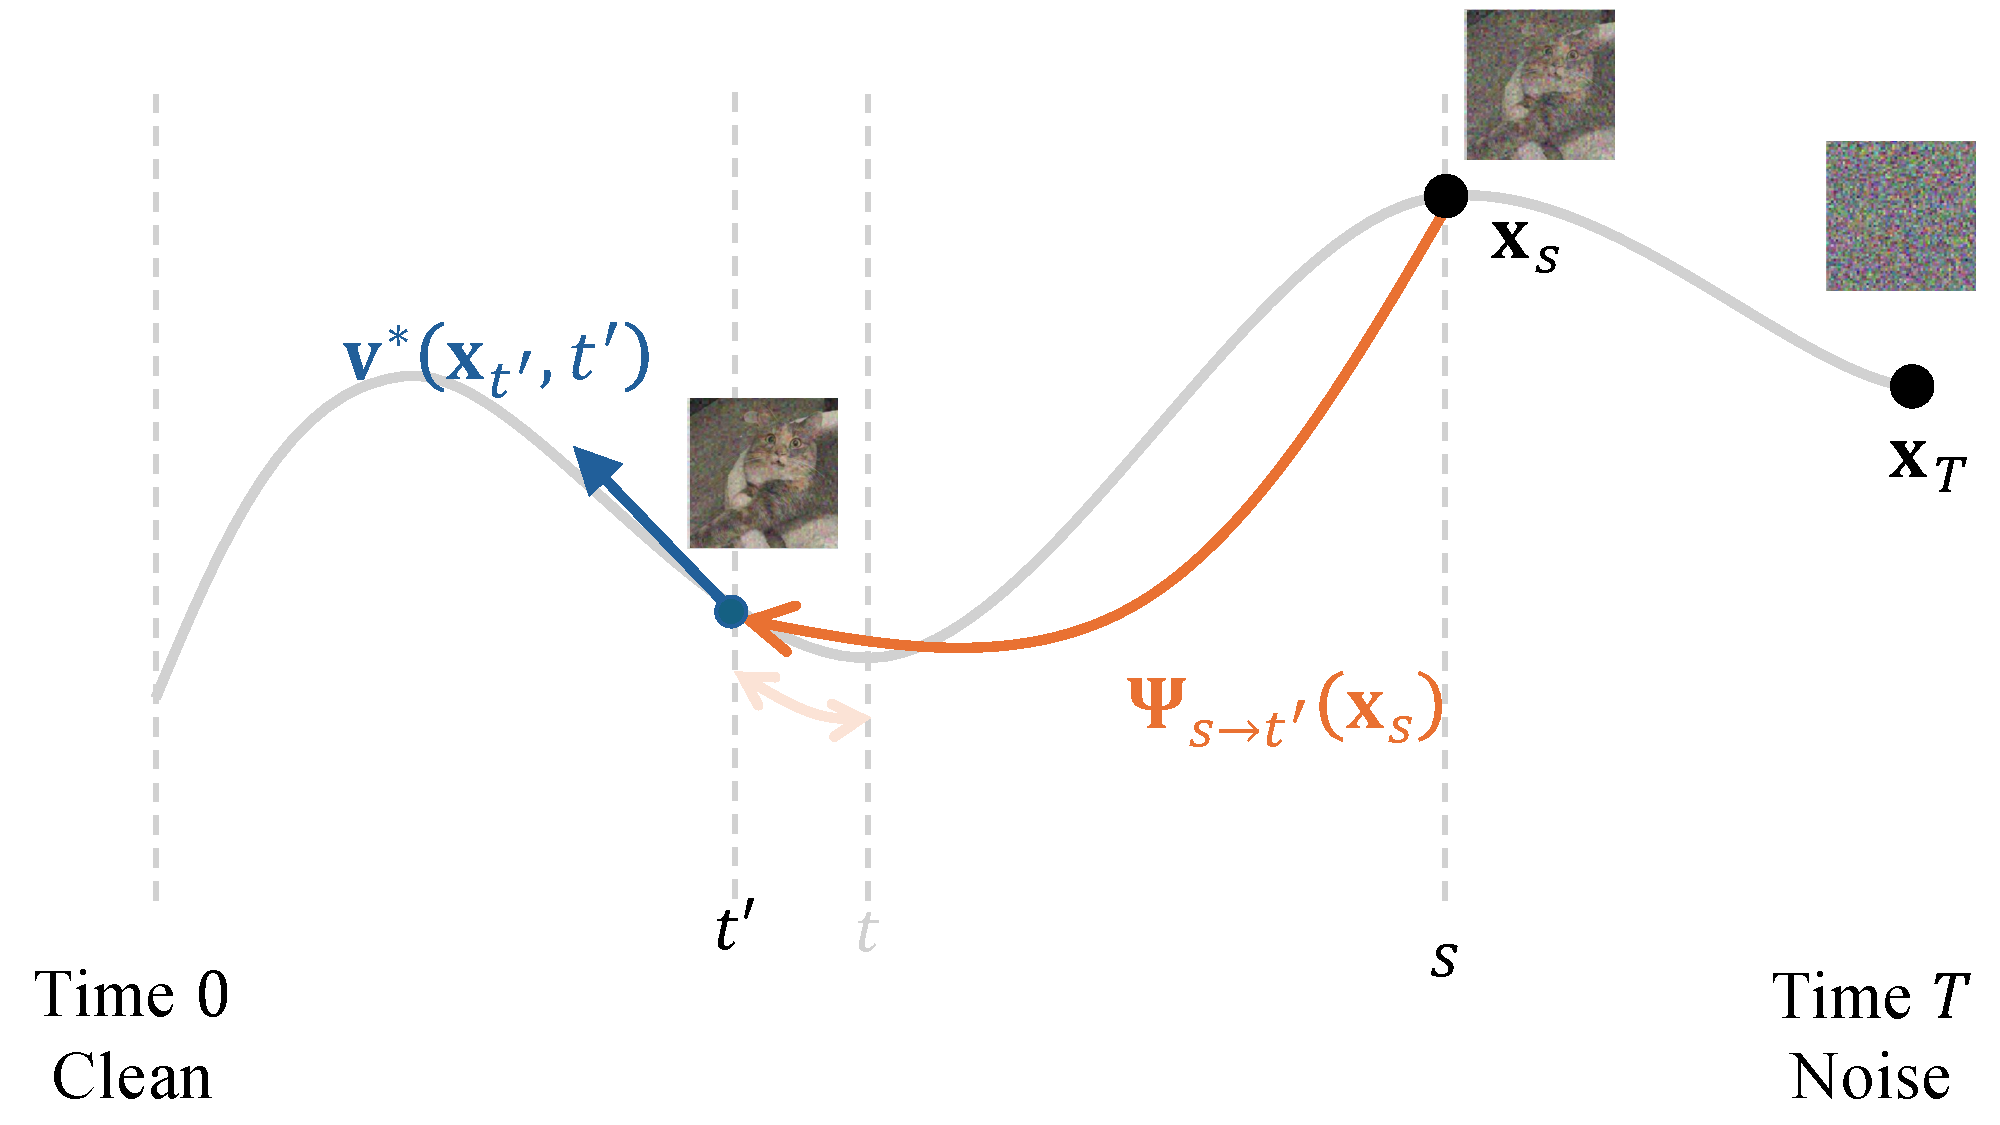
\includegraphics[width=\linewidth]{Images/PartD/lagrangian-2.pdf}
        \caption{移动后的目标时刻 $t'$。}
        \label{fig:lagrangian-moved}
    \end{subfigure}

    \caption{\textbfs{流映射的拉格朗日一致性。}
    源 $(\rvx_s,s)$ 固定，目标时刻从 $t$ 移动到
    $t'$。流映射的输出沿同一 PF-ODE 轨迹移动，其
    无穷小变化等于 ODE 速度：
    $\partial_t \bPsi_{s\to t}(\rvx_s)
    = \rvv^*(\bPsi_{s\to t}(\rvx_s),t)$。}
    \figcredit{改编自 \citet{dieleman2026flowmaps}。}
    \label{fig:lagrangian-consistency}
\end{figure}

\paragraph{拉格朗日视角：移动目的地。}
固定源 $(\rvx_s,s)$ 并移动目标时刻 $t$。预测的
终点应沿同一轨迹滑动：
\[
\partial_t \bPsi_{s\to t}(\rvx_s)
=
\rvv^*(\bPsi_{s\to t}(\rvx_s),t).
\]
“拉格朗日”这一名称源于经典的粒子视角：当目的地时刻变化时，我们追踪
轨迹上的一个移动点。在无穷小意义上，
终点以该终点处的局部 ODE 速度移动。

\paragraph{欧拉视角：移动源。}
固定目标时刻 $t$，并沿同一轨迹滑动源点。
时刻 $t$ 处的目的地保持不变：
\[
\frac{\diff}{\diff s}\bPsi_{s\to t}(\rvx_s)=0.
\]
由于 $\frac{\diff}{\diff s}\rvx_s=\rvv^*(\rvx_s,s)$，链式法则给出
\[
\partial_s\bPsi_{s\to t}(\rvx_s)
+
\big(\partial_{\rvx}\bPsi_{s\to t}\big)(\rvx_s)\rvv^*(\rvx_s,s)
=
0.
\]
“欧拉”这一名称反映了场视角：我们考察映射
如何随其源输入的变化而变化。对 CM 而言，目标是干净终点
$t=0$，且
\[
    \rvf^*(\rvx_s,s)=\bPsi_{s\to0}(\rvx_s).
\]
因此，\Cref{eq:conti-ct-motivation}是
\Cref{sec:discrete-cm,sec:conti-cm}中所研究的特殊流映射的源时刻一致性条件。



这一视角也回顾了\Cref{subsec:equivalence-ctm-mf}中
CTM 与 MF 之间的关系。两者都近似同一路径积分
\[
\bPsi_{s\to t}(\rvx_s)
=
\rvx_s+\int_s^t\rvv^*(\rvx_\tau,\tau)\,\diff\tau,
\]
但暴露出不同的可训练代理。CTM 通过
位移式参数化表示终点，而 MF 通过平均漂移表示同一终点
\[
\rvh^*(\rvx_s,s,t)
=
\frac{1}{t-s}\int_s^t\rvv^*(\rvx_\tau,\tau)\,\diff\tau.
\]
将
\[
\bPsi_{s\to t}(\rvx_s)=\rvx_s+(t-s)\rvh^*(\rvx_s,s,t)
\]
代入欧拉源时刻恒等式得到
\[
\rvh^*(\rvx_s,s,t)
=
\rvv^*(\rvx_s,s)
-
(s-t)
\left[
\partial_s\rvh^*(\rvx_s,s,t)
+
(\partial_{\rvx}\rvh^*)(\rvx_s,s,t)\rvv^*(\rvx_s,s)
\right].
\]
这就是基本的均值流恒等式：长区间上的平均漂移等于
源点处的瞬时漂移，再由平均漂移随源点沿同一轨迹滑动
的变化所修正。

\begin{figure}[t]
    \centering

    \begin{subfigure}[t]{0.485\textwidth}
        \centering
        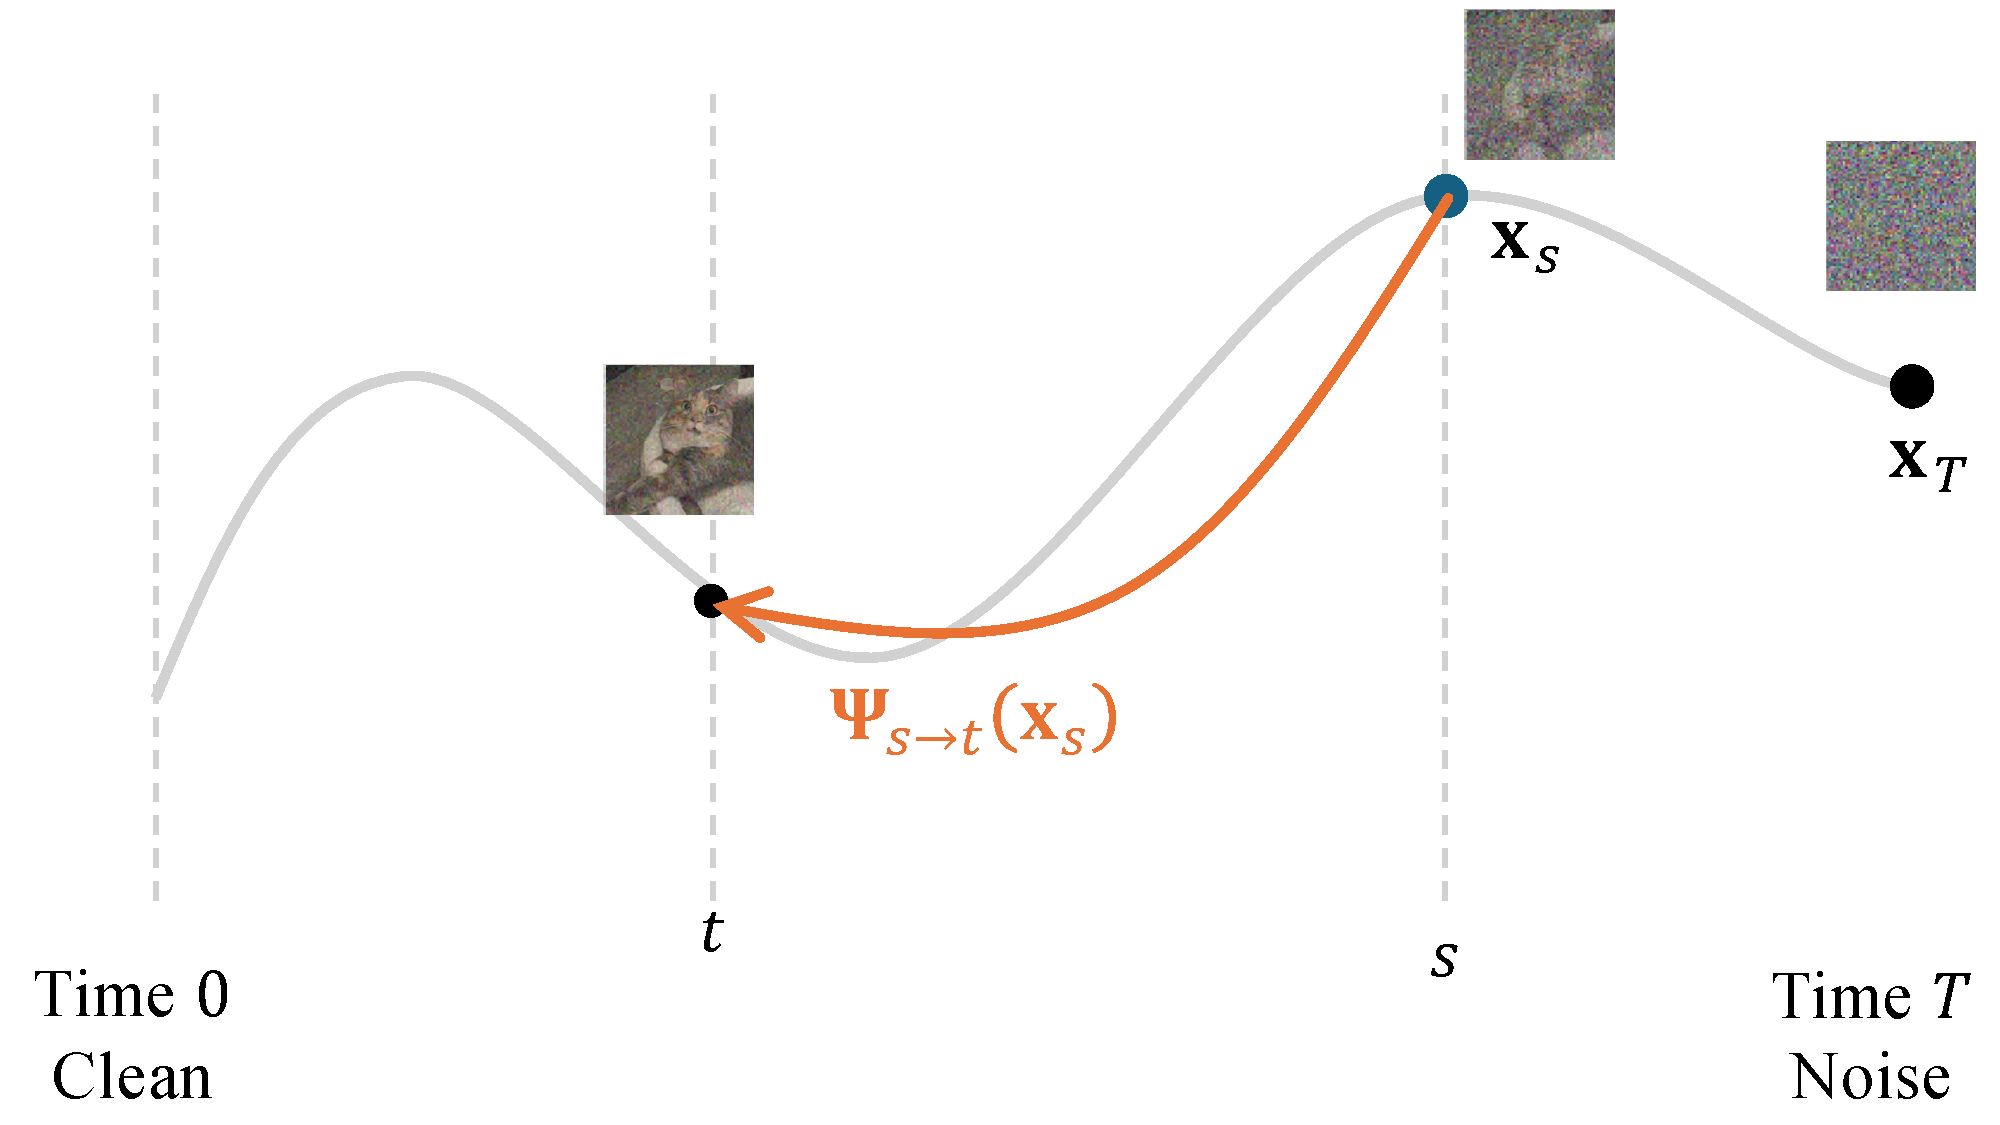
\includegraphics[width=\linewidth]{Images/PartD/eulerian-1.pdf}
        \caption{基准源时刻 $s$。}
        \label{fig:eulerian-base}
    \end{subfigure}
    \hfill
    \begin{subfigure}[t]{0.485\textwidth}
        \centering
        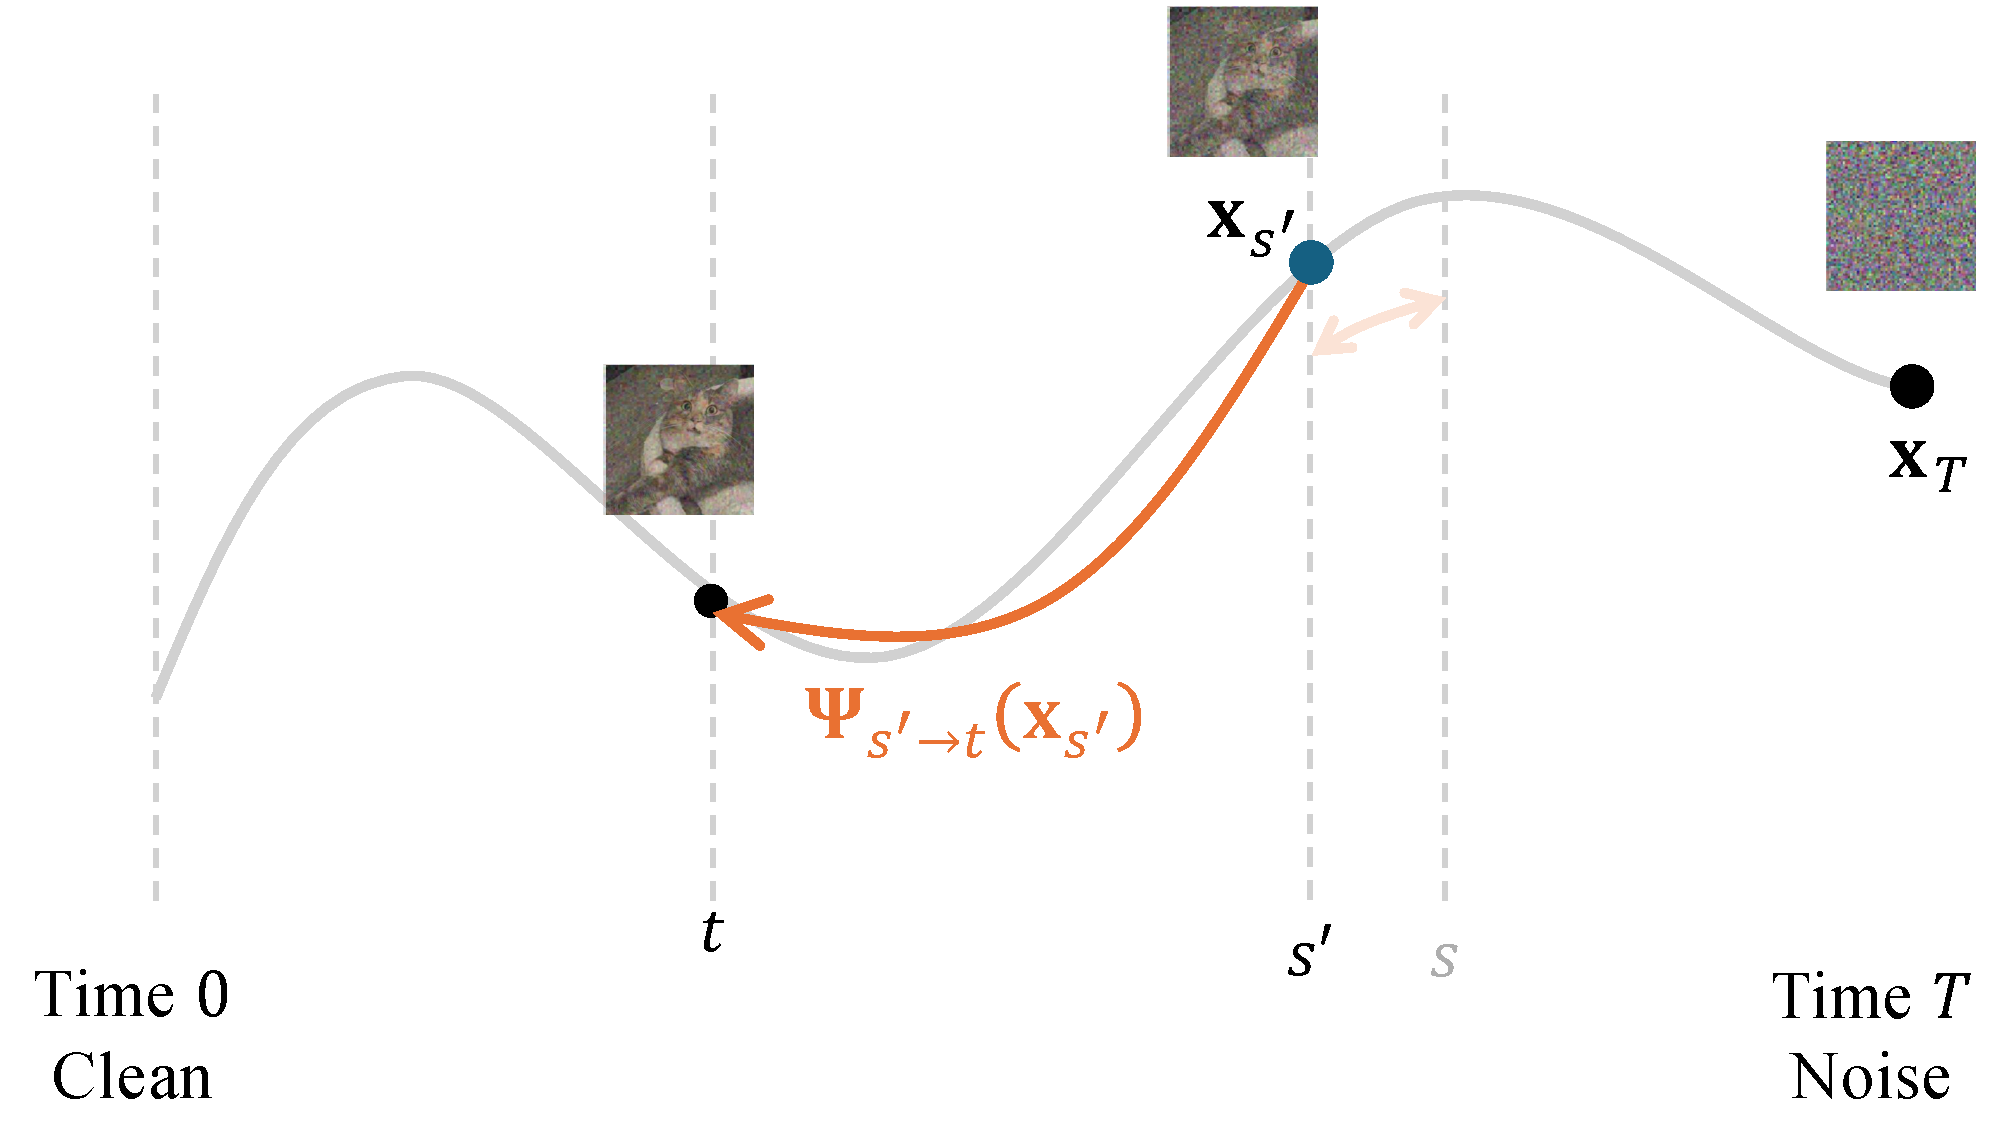
\includegraphics[width=\linewidth]{Images/PartD/eulerian-2.pdf}
        \caption{移动后的源时刻 $s'$。}
        \label{fig:eulerian-moved}
    \end{subfigure}

    \caption{\textbfs{流映射的欧拉一致性。}
    目标时刻 $t$ 固定，源时刻从 $s$ 移动到
    $s'$。由于源点位于同一 PF-ODE 轨迹上，流映射的
    输出应保持不变：
    $\bPsi_{s\to t}(\rvx_s)=\bPsi_{s'\to t}(\rvx_{s'})$。
    在无穷小意义上，这给出
    $\frac{\diff}{\diff s}\bPsi_{s\to t}(\rvx_s)=0$，或等价地
    $\partial_s\bPsi_{s\to t}(\rvx_s)
    +(\partial_{\rvx}\bPsi_{s\to t})(\rvx_s)\rvv^*(\rvx_s,s)=0$。}
        \figcredit{改编自 \citet{dieleman2026flowmaps}。}
    \label{fig:eulerian-consistency}
\end{figure}
\paragraph{三种视角的等价性。}
对于精确的 oracle 映射，半群、拉格朗日和欧拉视角是
同一 ODE 流映射的三种等价刻画~\citep{boffi2024flow}。
关键原理是 ODE 解轨迹的存在性与唯一性：
一旦状态-时刻对 $(\rvx_s,s)$ 固定，穿过它的轨迹就被
确定。

半群恒等式给出该原理的有限区间形式：
\[
    \bPsi_{u\to t}\big(\bPsi_{s\to u}(\rvx_s)\big)
    =
    \bPsi_{s\to t}(\rvx_s),
    \qquad
    \bPsi_{s\to s}=\rmI .
\]
两种微分视角通过收缩两个区间之一得到。

首先，收缩目标侧区间。对 $\Delta t>0$，
\[
    \bPsi_{t\to t-\Delta t}
    \big(\bPsi_{s\to t}(\rvx_s)\big)
    =
    \bPsi_{s\to t-\Delta t}(\rvx_s).
\]
令 $\rvx_t:=\bPsi_{s\to t}(\rvx_s)$。对短
流的一阶展开给出
\[
    \bPsi_{t\to t-\Delta t}(\rvx_t)
    =
    \rvx_t-\Delta t\,\rvv^*(\rvx_t,t)
    +\mathcal{O}\big((\Delta t)^2\big).
\]
因此，
\[
    \frac{
    \bPsi_{s\to t-\Delta t}(\rvx_s)
    -
    \bPsi_{s\to t}(\rvx_s)}
    {-\Delta t}
    =
    \rvv^*(\rvx_t,t)
    +\mathcal{O}(\Delta t).
\]
取 $\Delta t\to0$ 得到拉格朗日恒等式
\[
    \partial_t\bPsi_{s\to t}(\rvx_s)
    =
    \rvv^*\big(\bPsi_{s\to t}(\rvx_s),t\big).
\]
因此，当源 $(\rvx_s,s)$ 固定而目标时刻移动时，
预测终点以该终点处的 ODE 速度移动。

其次，收缩源侧区间。对 $\Delta s>0$，
\[
    \rvx_{s-\Delta s}
    :=
    \bPsi_{s\to s-\Delta s}(\rvx_s)
    =
    \rvx_s-\Delta s\,\rvv^*(\rvx_s,s)
    +\mathcal{O}\big((\Delta s)^2\big).
\]
半群恒等式给出
\[
    \bPsi_{s-\Delta s\to t}(\rvx_{s-\Delta s})
    =
    \bPsi_{s\to t}(\rvx_s).
\]
对左侧在源状态和源时刻上同时展开给出
\[
    \bPsi_{s-\Delta s\to t}(\rvx_{s-\Delta s})
    =
    \bPsi_{s\to t}(\rvx_s)
    -
    \Delta s\,
    \big(\partial_{\rvx}\bPsi_{s\to t}\big)(\rvx_s)\rvv^*(\rvx_s,s)
    -
    \Delta s\,
    \partial_s\bPsi_{s\to t}(\rvx_s)
    +
    \mathcal{O}\big((\Delta s)^2\big).
\]
与半群恒等式比较并除以 $-\Delta s$ 得到
\[
    \partial_s\bPsi_{s\to t}(\rvx_s)
    +
    \big(\partial_{\rvx}\bPsi_{s\to t}\big)(\rvx_s)\rvv^*(\rvx_s,s)
    =
    \mathcal{O}(\Delta s).
\]
取 $\Delta s\to0$ 得到欧拉恒等式
\[
    \partial_s\bPsi_{s\to t}(\rvx_s)
    +
    \big(\partial_{\rvx}\bPsi_{s\to t}\big)(\rvx_s)\rvv^*(\rvx_s,s)
    =
    0.
\]
这里目标时刻 $t$ 固定，而源点沿同一
轨迹移动，因此预测目的地保持不变。

反之，任一微分恒等式连同边界条件 $\bPsi_{s\to s}=\rmI$ 都恢复同一
流映射。拉格朗日恒等式从
$\bPsi_{s\to s}(\rvx_s)=\rvx_s$ 演化终点。欧拉恒等式表明
$\bPsi_{\tau\to t}(\rvx_\tau)$ 沿特征线
$\rvx_\tau=\bPsi_{s\to \tau}(\rvx_s)$ 为常数，故
\[
    \bPsi_{s\to t}(\rvx_s)
    =
    \bPsi_{t\to t}(\rvx_t)
    =
    \rvx_t.
\]
尽管这些视角在 oracle 层面等价，但一旦引入近似，它们会导致
不同的实用算法：必须
选择强制执行哪个恒等式、停梯度目标放在哪里、如何
采样时间对、以及如何参数化映射。


\paragraph{总结。}
流映射模型汇集了本书各处发展的若干原理。其概念转变是
直接学习 PF-ODE 的解映射：模型不再在采样时反复查询
局部速度场并逐步积分，而是试图将这部分积分摊销到训练中。

这一转变为单步和少步生成提供了一条有原则的路径。
当学习到的映射准确时，生成轨迹的长区间可以
仅用少量网络求值即可遍历，同时
仍然与扩散的轨迹式结构保持联系。在这个意义上，
流映射学习在迭代
扩散过程的样本质量与直接生成器的速度之间架起了一座桥梁。

代价是负担从采样转移到了学习。模型必须
近似比瞬时速度场更全局的对象，其
性能取决于参数化、时间采样、损失
加权、停梯度放置和稳定化的精心选择。
从这个角度看，从零开始学习快速生成器是基于扩散的生成式建模故事的
自然延续。它保留了使扩散模型可靠的数学
结构，同时为高效、可控、有原则的生成开启了更广阔的设计
空间。目标不再仅仅是更快地求解生成式 ODE，而是学习其
解算子本身有用的片段。



% \section{Closing Remarks}\label{sec:ch11_cr}

% This final chapter has brought our exploration full circle, culminating in a new paradigm for generative modeling: learning fast, few-step generators from scratch. Moving beyond the approaches of improving numerical solvers or distilling pre-trained models, we have focused on designing standalone training principles that are both principled and highly efficient by design.

% The core innovation presented here is the direct learning of the flow map ($\bm{\Psi}_{s\rightarrow t}$) of the underlying probability flow ODE. The key to making this tractable without a teacher was leveraging the fundamental semi-group property of the ODE flow. This property, which dictates that a long trajectory can be decomposed into shorter segments, provides a powerful self-supervisory signal for training.

% We began with Consistency Models (CMs), which pioneered this approach by learning the special flow map that transports any noisy state back to its clean origin ($\bm{\Psi}_{s\rightarrow 0}$). We then saw this idea generalized by Consistency Trajectory Models (CTM) and Mean Flow (MF), which learn the complete, anytime-to-anytime flow map $\bm{\Psi}_{s\rightarrow t}$ for all $s,t$ satisfying $s\ge t$. While appearing different in their parameterization, we showed that these methods are fundamentally equivalent ways of approximating the same path integral that defines the flow map.

% These flow map models represent a powerful synthesis of the principles developed throughout this book. They inherit the continuous-time foundation of the Score SDE framework and the deterministic transport view of Flow Matching, but reformulate the training objective to be self-contained and efficient.

% By learning the solution map directly, these standalone models successfully unite the high sample quality of iterative diffusion processes with the inference speed of one-step generators. They resolve the fundamental trade-off between fidelity and speed, marking a significant milestone in generative modeling. This achievement represents not an end, but the beginning of a new chapter in the design of powerful, efficient, and controllable generative AI.



% Diffusion models may at first appear as a collection of many acronyms and variants, yet their underlying idea is remarkably simple. At a high level, they provide mechanisms for \emph{transporting probability mass} from a simple reference distribution, such as Gaussian noise, to a complex data distribution over time. From this perspective, generation can be viewed as the evolution of a \emph{cloud of particles}, and the mathematical structure becomes much less mysterious: it is fundamentally a problem of \emph{time-dependent change of variables}. In continuous time, deterministic motion of particles leads to the continuity equation, while motion with additional random perturbation leads to the Fokker-Planck equation. Many seemingly different formulations can be understood as variations built on this common foundation.

% At the same time, the classical strength of diffusion models, namely their ability to generate \emph{high-fidelity} samples, is closely tied to a classical weakness: \emph{iterative sampling}. When the reverse dynamics must be integrated through many small steps, generation remains computationally slow. Flow map models extend the same basic viewpoint in a natural direction. Rather than learning only infinitesimal updates and then numerically integrating them, they seek to learn the \emph{time-jump maps} of the probability-flow ODE (PF-ODE) directly. That is, they aim to approximate the flow map
% \[
% \Psi_{s\to t},
% \]
% so that a long chain of small updates may be replaced by a small number of large but accurate transitions. Consistency Models (CM), Consistency Trajectory Models (CTM), and Mean Flow (MF) provide three concrete examples of this idea. Each imposes a different structural principle on the flow map, such as consistency, semigroup structure, or mean-slope identities, in order to construct practical training targets when the exact flow map is unavailable.

% Stepping back, the main message is encouraging. Diffusion is not merely a single method, but a \emph{general principle for constructing generators} from a prescribed forward process. Once we adopt the viewpoint of first choosing a forward corruption mechanism and then learning the corresponding reverse transport, a wide range of designs becomes possible, each balancing \emph{stability}, \emph{sample quality}, and \emph{generation speed} in different ways. Flow map models represent one promising direction, but they are unlikely to be the final answer. The broader opportunity is to preserve the same clean backbone: define a forward transport process, understand how the distribution evolves through change of variables, and then develop new \emph{parameterizations} and \emph{training objectives} that make \emph{fast generation} as reliable as the best step-by-step samplers.


%%%%%%%%%%%%%%%%%%%%%%%%%%%%%%%%%%%%%%%%%%%%%%%%%%%%%%%%%%%%%%%%%%%%%%%%
\clearpage
\newpage
%%%%%%%%%%%%%%%%%%%%%%%%%%%%%%%%%%%%%%%%%%%%%%%%%%%%%%%%%%%%%%%%%%%%%%%%





\part*{结语与展望}
\addcontentsline{toc}{part}{结语与展望}
\chapter{结语与展望}\label{ch:epilogue}

\epigraph{\textit{抽象的目的不是要含糊其辞，而是要创造一个新的语义层次，在其中可以做到绝对精确。}}{Edsger W.\ Dijkstra}

本书的每一章都在讨论同一件事：概率质量在某种预设变换下如何流动，以及如何逆转、近似或利用这种流动来生成数据。在这最后一章中，我们退后一步，把这种结构上的统一性明确地呈现出来。我们首先回顾支撑前述全部内容的变量替换原理（\Cref{sec:epilogue-backbone}），然后说明同样的概率传输视角如何通过马尔可夫核和连续时间马尔可夫链扩展到离散状态空间（\Cref{sec:epilogue-discrete}），最后对更广阔的图景作若干反思（\Cref{sec:epilogue-closing}）。

\clearpage
\newpage

\section{密度传输的主干}\label{sec:epilogue-backbone}

在全书之中，我们沿着两条紧密相关的发展线索展开。
第一条线索是\emph{扩散模型本身}，包括变分、基于分数和基于流这几种形式，它们为概率律如何演化、以及如何为了生成而逆转这种演化提供了不同的数学描述。
第二条线索是\emph{受扩散启发的快速生成器}，其中最具代表性的是流映射模型（flow map models），它们建立于同样的传输视角之上，但旨在学习更直接、更高效的生成器。
尽管形式各异，所有这些方法都根植于同一个组织性思想：生成式建模从本质上讲是一个\emph{传输概率质量}的问题。从一个简单的参考分布（例如高斯噪声）出发，我们设法构造一个过程，逐步把它与复杂的数据分布联系起来。

这种视角之所以有用，是因为它把注意力从单个模型族移开，引向一个更根本的问题：
\emph{当底层样本被某种预设的动力学所驱动时，概率律会如何演化？}
回答这一问题的数学语言，就是变量替换公式及其连续时间推广。从这个意义上说，变量替换原理不仅是一种技术工具，它更是扩散模型及其所启发的快速生成器共同的概念主干。

\paragraph{共同的三步结构。}
在较高的层面上，本书所研究的方法都遵循同样一个简单的模式：
\begin{enumerate}[leftmargin=2em]
    \item 定义一个前向过程，逐步把数据推向一个简单的参考分布。
    \item 通过适当的定律演化方程，理解概率律在该过程下如何演化。
    \item 学习一个生成机制，使之逆转、近似或以其他方式利用这种演化，从而产生样本。
\end{enumerate}
不同形式之间的差别，仅在于前向过程的选择、定律演化方程的数学形式，以及生成机制被参数化和训练的方式。

\paragraph{变量替换的层级体系。}
在 \Cref{app:continuity} 中，我们系统地推导了变量替换公式的一个递进体系，从确定性双射到随机微分方程。这一递进关系值得在此回顾，因为它揭示了同一种传输原理以若干不同形式出现。

\FloatBarrier % ensures figures above don’t float past here

\begin{figure}[H]
  \centering

  % --- First row ---
  \begin{subfigure}{\textwidth}
    \centering
    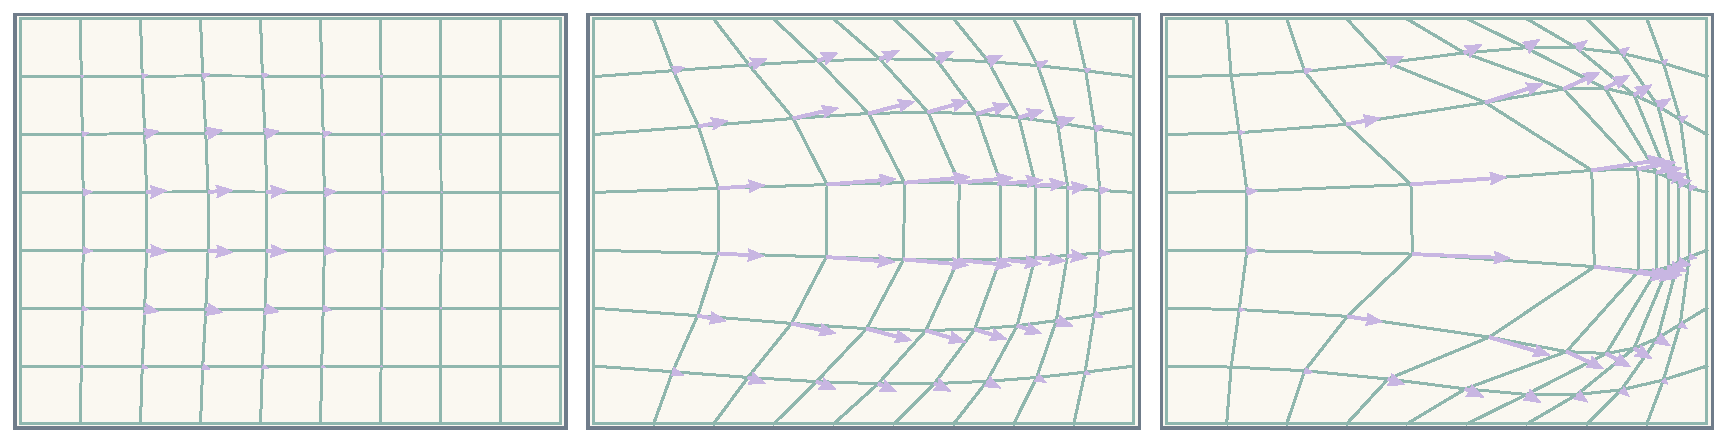
\includegraphics[width=\textwidth]{Images/appendix/vector_field_only.pdf}
        \caption{向量场示意图。箭头代表驱动粒子在空间中运动的力，相应地使底层网格发生形变。}
  \end{subfigure}

  \vspace{0.5em} % space between rows

  % --- Second row ---
  \begin{subfigure}{\textwidth}
    \centering
    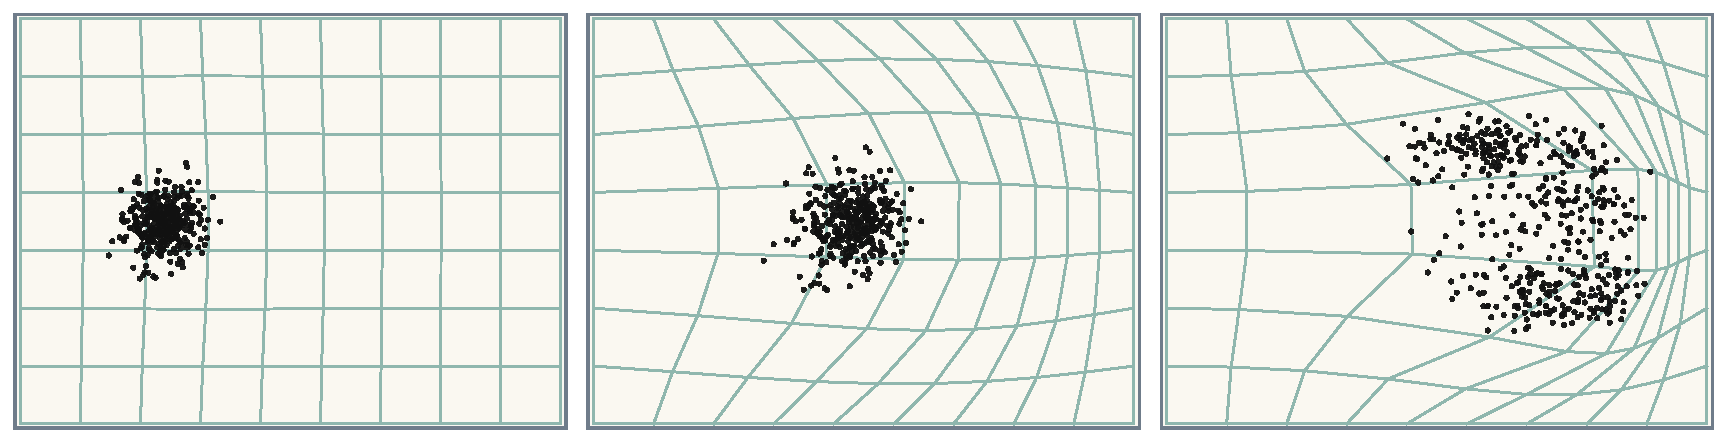
\includegraphics[width=\textwidth]{Images/appendix/particle_cloud.pdf}
    \caption{粒子云动力学。将一个预定义的向量场解释为力，它生成一个流，把粒子从其初始状态传输出去。}
  \end{subfigure}

  \vspace{0.5em}

  % --- Third row ---
  \begin{subfigure}{\textwidth}
    \centering
    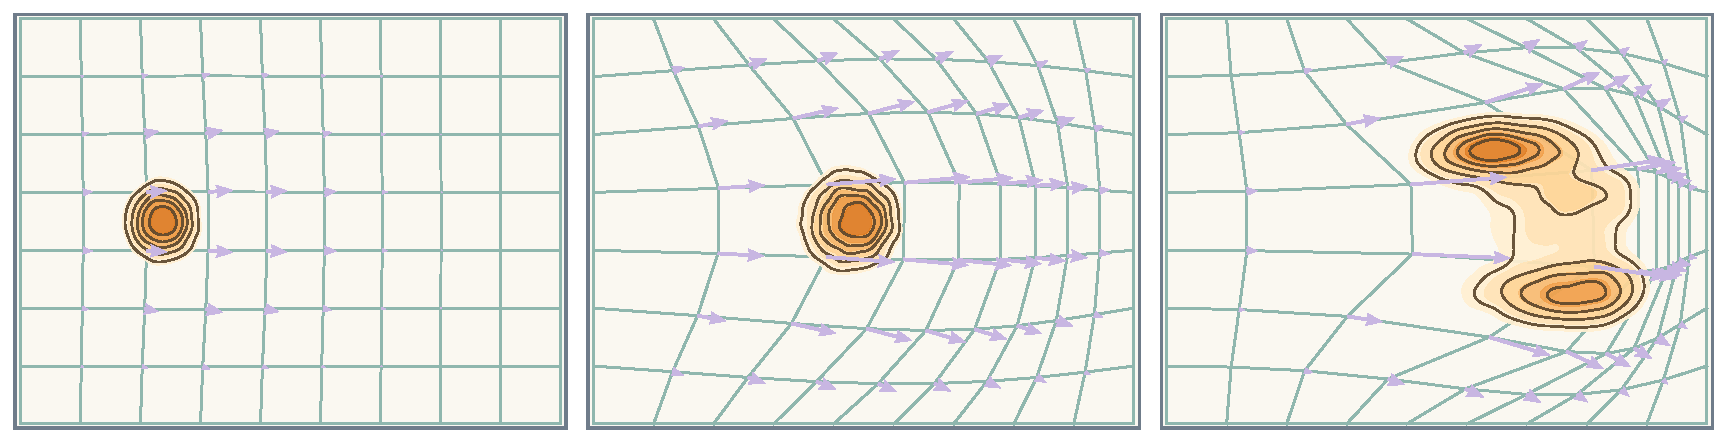
\includegraphics[width=\textwidth]{Images/appendix/vector_field_with_density.pdf}
    \caption{密度演化。当粒子被向量场平流输送时，密度等值线随之形变，反映出流如何重塑底层分布。}
  \end{subfigure}

  \caption{\textbfs{向量场下粒子与密度动力学示意图。}
每一列从左到右依次展示连续的时间快照。\figcredit{改编自 \citet{lipman2024flow}。}
}
  \label{fig:flow-3x3rows}
\end{figure}

\begin{enumerate}[leftmargin=2em]
    \item \textbfs{单个双射。}
    一个光滑可逆映射 $\bPsi:\R^D\to\R^D$ 通过下式把密度 $p_0$ 变换为 $p_1$：
    \[
    p_1(\rvx_1)
    =
    p_0\bigl(\bPsi^{-1}(\rvx_1)\bigr)
    \left|\det \partial_{\rvx_1}\bPsi^{-1}(\rvx_1)\right|.
    \]
    Jacobi 行列式记录了局部的体积变化：当映射拉伸空间时，密度减小；当它压缩空间时，密度增大。

    \item \textbfs{复合双射。}
    把许多双射链接起来，令 $\rvx_k=\bPsi_k(\rvx_{k-1})$，得到
    \[
    \log p_L(\rvx_L)
    =
    \log p_0(\rvx_0)
    -
    \sum_{k=1}^L
    \log\left|\det \partial_{\rvx_{k-1}}\bPsi_k(\rvx_{k-1})\right|.
    \]
    这是归一化流背后的基本原理。更重要的是，它已经阐明了核心信息：一旦粒子运动被确定，密度的演化便随之确定。

    \item \textbfs{连续时间确定性流（ODE）。}
    取无穷小步长的极限，便得到连续性方程，
    \[
    \frac{\partial p_t(\rvx)}{\partial t}
    +
    \nabla\cdot\bigl(p_t(\rvx)\,\rvv(\rvx,t)\bigr)
    =
    0,
    \]
    其中粒子按如下方式演化
    \[
    \frac{\diff \rvx(t)}{\diff t} = \rvv(\rvx(t),t).
    \]
    这是质量守恒的连续时间表达。概率质量既不会被创造也不会被消灭，它只是在速度场 $\rvv$ 之下在空间中流动。

    \item \textbfs{连续时间随机流（SDE）。}
    加入布朗噪声，便得到 Fokker--Planck 方程，
    \[
    \frac{\partial p_t(\rvx)}{\partial t}
    =
    -\nabla\cdot\bigl(\rvv(\rvx,t)\,p_t(\rvx)\bigr)
    +
    \frac{1}{2}g^2(t)\,\Delta p_t(\rvx),
    \]
    它对应于如下的随机动力学
    \[
    \diff\rvx(t) = \rvv(\rvx(t),t)\diff t + g(t)\diff\rvw(t).
    \]
    第一项描述由漂移项驱动的定向传输，第二项刻画噪声引起的随机扩散。
\end{enumerate}

这些并不是互不相关的公式。
多层变量替换法则是重复的确定性变换下传输的离散时间版本。
其无穷小的确定性极限给出连续性方程。
加入随机扰动则导出 Fokker--Planck 方程。
每一层都是对前一层的推广，同时保留了同一个底层原理：概率质量守恒，概率律据此调整，以反映底层动力学如何驱动样本在空间中运动。

从这一视角出发，本书中的主要形式便更容易在整体中定位。
变分方法通过时间网格上的去噪转移来描述生成。基于分数的方法则处理随机动力学，并学习控制逆向时间 SDE 的分数场。
基于流的方法处理确定性传输，并学习一个速度场，其轨迹遵循同一族中间定律。
而快速生成器则建立在这同一主干之上，但寻求更直接的方式来利用所学到的传输以进行高效采样。

因此，核心结论十分简单。
扩散建模最好不应被理解为某个绑定于单一架构或单一噪声调度的单一算法。它是一种\emph{设计原理}：指定一个前向传输过程，理解由此引起的概率律演化，然后在这一结构之上构造一个生成器。一旦确立了这种视角，许多看似不同的方法便成为同一思想的不同自然变体。

随之产生一个自然的问题：这一原理是否可以推广到连续状态空间之外？在下一节中，我们将说明确实如此。

\clearpage
\newpage


\section{超越连续状态：离散空间上的概率演化}
\label{sec:epilogue-discrete}

到目前为止，本书中出现的每一个模型都共享一个共同的结构
假设：生成动力学所作用的状态处于
连续的欧几里得空间 $\R^D$ 之中。不论 $\rvx$ 的各分量代表
像素强度、音频采样还是连续的隐变量，其
数学都是相同的：粒子沿着由 ODE 或 SDE 所支配的连续轨迹运动，而概率密度则通过连续性或
Fokker--Planck 方程演化。这一框架建立在 $\R^D$ 的微分结构之上：梯度与
散度通过导数来定义，确定性动力学可由向量场生成的可微轨迹来描述。

这种区别关乎的是建模所用的状态，而非原始的模态。
离散的观测也可以通过先选择一个连续的编码
和一个读出来处理。对于一个原始符号 $a$，令 $\rmE(a)\in\R^d$ 为其编码，
并令 $\rmD$ 把编码映射回符号，或者更一般地映射到一个
类别分布：
\[
\text{raw discrete symbol } a
\;\xrightarrow{\;\rmE\;}\;
\text{continuous code } \rmE(a)\in\R^d
\;\xrightarrow{\;\rmD\;}\;
\text{discrete readout}.
\]
该表示可以是固定的，例如 one-hot、类别向量或
单纯形取值的编码~\citep{richemond2022categorical}；
在单射码本上，读出可以是确定性的，并可能满足
$\rmD(\rmE(a))=a$。另一种选择是，该表示也可以是学习得到的，
例如词元嵌入或自编码器的隐表示
\citep{li2022diffusionlm,dieleman2022continuous}；此时 $\rmD$ 是一个学习得到的
读出，$\rmD\circ\rmE$ 也不必精确可逆。一旦
表示被固定下来，扩散过程便是连续状态的：在周围编码空间中的高斯加噪，或在受限编码空间中采用几何适配的连续过程，都可以用本书前文所发展的连续机制来处理。下文研究的有限状态路径则不同：演化的状态本身始终保持离散。

本节研究的是与之互补的情形，即在整个前向和反向过程中，状态本身
始终是有限且离散的。许多数据类型天然符合这一视角：文本是词表词元的序列，分子图使用有限多种原子类型和键类型，
蛋白质序列是有限字母表上的字符串。在这样的有限状态
空间中，从一个状态到另一个状态之间不存在规范的无穷小位移，
不存在穿越词元取值的光滑轨迹，也不存在关于状态本身的普通梯度。这自然引出一个问题：
\begin{question}
    如果扩散确实是关于传输概率质量的，那么当状态空间有限时，这一想法会变成什么？
\end{question}

结构主干保持不变，但数学对象发生了变化。
在连续空间中，概率律通过 ODE/SDE 动力学在连续性或
Fokker--Planck 方程下演化。在有限状态空间中，概率质量
按照马尔可夫转移核或跳变速率在状态之间转移，
而定律则由一个有限维的守恒律——即\emph{主方程}，也称为 Kolmogorov 前向方程——所演化。在抽象层面上，
两种设定都遵循同样的配方：

\msg{观察}{}{选择一个前向破坏过程，理解其诱导的概率路径，并学习一个反向传输机制。}

在连续高斯扩散中，这种反向机制表现为高斯
反向条件分布、分数或速度场。在有限状态空间中，它
则表现为反向转移概率、概率比率或跳变
速率。它们是不同的数学对象，但扮演着相同的概念角色。

本章的目标并不在于把某一种离散扩散算法奉为定论。
相反，我们要发展出一份即使文献更迭也应当保持稳定的路线图。该路线图按照用来描述反向传输的对象来组织：转移核、概率比率或跳变速率。我们分四步展开：离散时间转移（\Cref{subsec:epilogue-dtmc}）、其连续时间极限（\Cref{subsec:epilogue-ctmc}）、与连续情形下变分、分数/比率和流三种视角相对应的三种反向建模视角（\Cref{subsec:epilogue-three-views}），以及对离散与连续情形之间真正差异的比较（\Cref{subsec:epilogue-genuine-diff}）。

\subsection{离散时间转移}
\label{subsec:epilogue-dtmc}

考虑一个在 $K$ 个离散类别上的前向过程，其中 $K$
包括所选前向过程所需的任何特殊破坏词元，例如掩码词元。每个状态表示为一个
\emph{one-hot} 列向量 $\rvx\in\{0,1\}^{K}$，其中恰好有一个
分量等于~$1$；所有这种向量的集合为\footnote{在 CTMC 与随机过程文献~\citep{norris1998markov,kelly1979reversibility} 中的一种等价表述，把每个状态表示为一个标量索引 $x\in\{1,\dots,K\}$，把转移
速率写作 $[\rmQ_t]_{ij}$，把边缘分布写作 $p_t(x)$。这里所采用的 one-hot 编码在记号上等价，但更贴近离散扩散文献~\citep{austin2021structured,sahoo2024simple,lou2024discrete}，其中诸如 $\langle\rvx_{\bphi},\rvx\rangle$ 的内积和
诸如 $\rmP^{\top}\rvx$ 的矩阵--向量乘积会自然出现在
训练目标中。}
\[
\mathcal{V}
= \bigl\{\rvx\in\{0,1\}^{K}:\textstyle\sum_{i=1}^{K}x_i=1\bigr\}
= \{\rve_1,\ldots,\rve_K\}.
\]
我们把 $\rve_i$ 记作第 $i$ 个标准基向量，即类别~$i$ 的 one-hot
编码。例如，每个 $\rve_i$ 可以代表
一个词元、一个离散隐码、一种原子类型、一种键类型或一种氨基酸。

对于文本或蛋白质等序列数据，一个样本由 $N$
个词元组成，每个词元在大小为~$K$ 的词表中取值。完整的状态空间便是 $\mathcal{V}^N$，其规模随序列长度呈指数增长。在许多离散扩散模型中，\emph{前向}破坏在各个位置上独立作用，因此单词元的马尔可夫过程便是基本的局部构件。我们先聚焦于单个词元，因为这能揭示核心的概率传输机制而不带来记号上的负担。对于完整序列，同样的公式可应用于完整构型，或者在前向破坏可分解时按位置分解。然而，学习得到的反向模型不必在各位置间独立：Transformer 或图神经网络可以观察整个被破坏的对象，并利用全局上下文来预测局部或全局的反向转移。

\begin{figure}[th!]
    \centering
    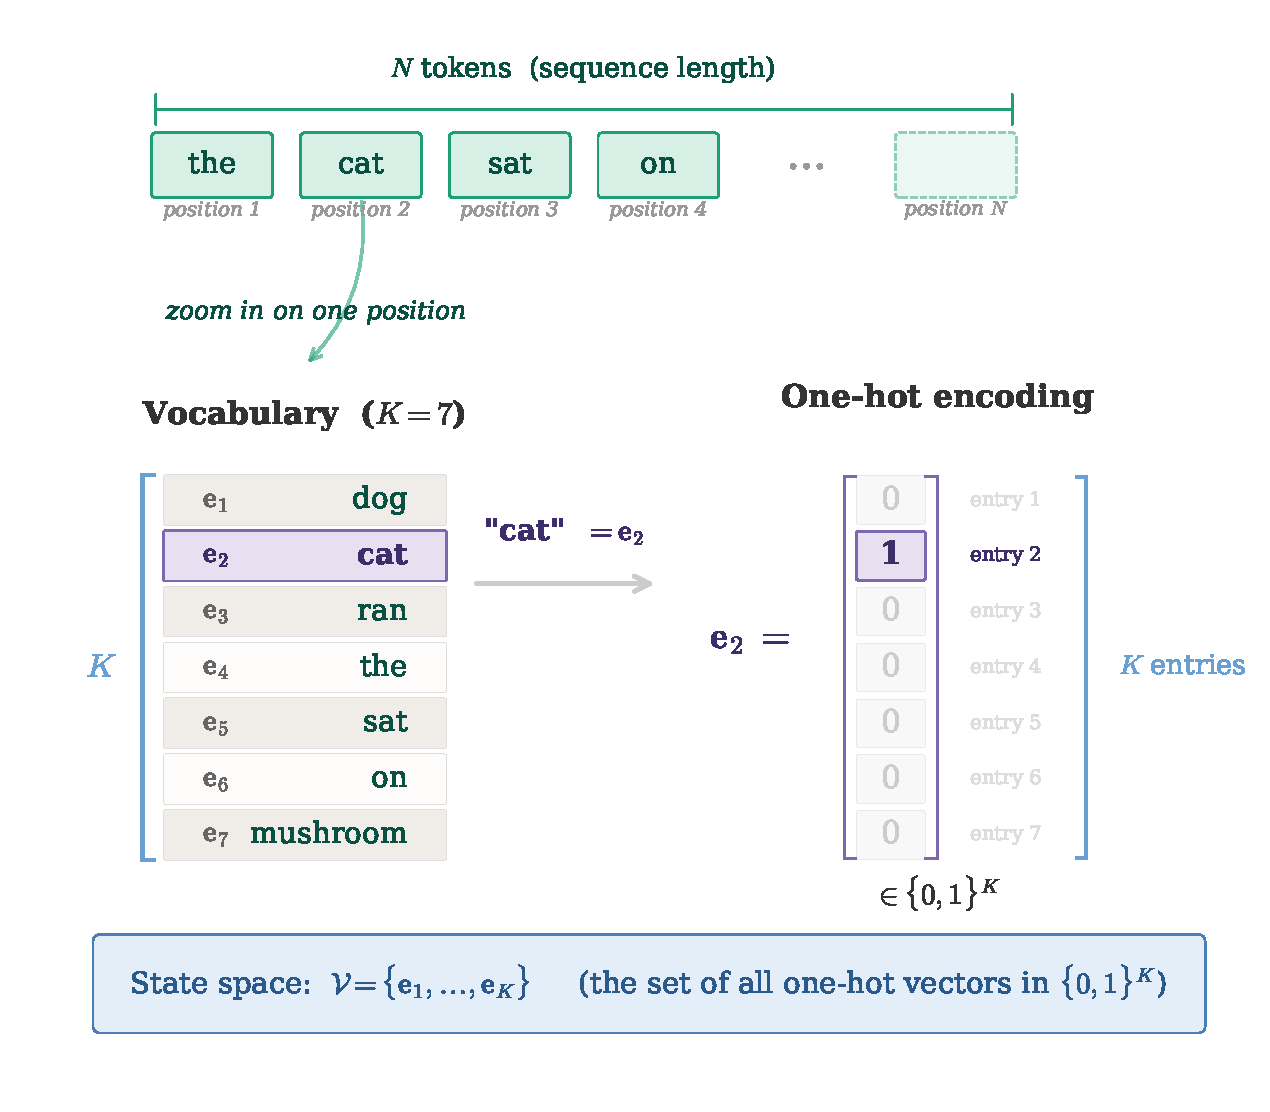
\includegraphics[width=\linewidth]{Images/PartE/fig_notation_overview.pdf}
    \caption{\textbfs{从序列到 one-hot 状态。}
    诸如文本或蛋白质序列这样的数据样本由 $N$
    个词元构成，每个词元在大小为~$K$ 的有限字母表或词表中取值。本章聚焦于
    单个词元在 $K$ 个状态之间的演化。放大观察某个位置，
    这里是 ``cat''，该词元由基向量
    $\rve_2$ 表示，并被编码为 $\{0,1\}^K$ 中的一个 one-hot 向量，即一个
    $K$ 维向量，其第二个分量为~$1$，其余所有
    分量均为~$0$。状态空间
    $\mathcal{V}=\{\rvx\in\{0,1\}^K:\sum_{i=1}^K x_i=1\}
    =\{\rve_1,\ldots,\rve_K\}$ 是所有这种 one-hot 向量的集合。
    词表条目的排序是任意的，与词元在序列中的位置无关。\figcredit{由作者在 AI 辅助编程下绘制。}}
    \label{fig:notation-overview}
\end{figure}

在第~$k$ 步，系统占据这 $K$ 个状态之一。我们把处于
状态~$\rve_i$ 的标量概率记为
\[
p_k(i) := \Pr(\rvx_k=\rve_i),
\qquad i=1,\ldots,K.
\]
收集这些标量概率，便得到边缘概率向量
\[
\rvp_k
:=
\bigl(p_k(1),\;\dots,\;p_k(K)\bigr)^\top
=
\E[\rvx_k]
\in \Delta^{K-1}\subset\R^K,
\qquad
\sum_{i=1}^K p_k(i)=1,
\]
其中 $\Delta^{K-1}:=\bigl\{\rvp\in\R^K:p_i\geq0,\;
\sum_{i=1}^K p_i=1\bigr\}$ 表示概率单纯形。
等价地，$\Pr(\rvx_k=\rve_i)=p_k(i)$，或简记为
$\rvx_k\sim\mathrm{Cat}(\rvp_k)$。

因此 $\rvp_k$ 是离散随机状态 $\rvx_k$ 的完整定律，而
$p_k(i)$ 是其第 $i$ 个标量分量。在连续时间下，我们沿用同一约定：
\[
p_t(i):=\Pr(\rvx_t=\rve_i),
\qquad
\rvp_t:=\bigl(p_t(1),\ldots,p_t(K)\bigr)^\top.
\]
向量 $\rvp_t$ 是密度的离散类比：它告诉我们总概率
质量如何在 $K$ 个状态之间分布。

按照全书使用的约定，粗体小写字母
（$\rvp$、$\rvx$）表示向量，粗体大写字母（$\rmP$、$\rmQ$）
表示矩阵，而不加粗的带下标量，如 $p_k(i)$、
$[\rmP_k]_{ij}$ 和 $[\rmQ_t]_{ij}$，表示标量分量。不加粗的
$p$ 以随机变量为自变量，如
$p(\rvx_{k-1}|\rvx_k)$，表示在固定前向过程下的概率质量函数或转移
核；$p_{\bphi}$ 表示学习得到的反向模型。



系统如何在状态之间转移？单步转移由一个
\emph{转移矩阵} $\rmP_k \in \R^{K \times K}$ 给出。
其元素 $[\rmP_k]_{ij}$ 给出当前处于
状态~$\rve_i$ 的系统在一步之内转移到状态~$\rve_j$ 的概率：
\[
[\rmP_k]_{ij} \;=\; \Pr(\rvx_{k+1} = \rve_j | \rvx_k = \rve_i).
\]
因此完整的矩阵具有如下结构：
\[
\rmP_k \;=\;
\underbrace{
\begin{pmatrix}
[\rmP_k]_{11} & [\rmP_k]_{12} & \cdots & [\rmP_k]_{1K} \\
[\rmP_k]_{21} & [\rmP_k]_{22} & \cdots & [\rmP_k]_{2K} \\
\vdots & \vdots & \ddots & \vdots \\
[\rmP_k]_{K1} & [\rmP_k]_{K2} & \cdots & [\rmP_k]_{KK}
\end{pmatrix}
}_{\substack{\text{columns: next state } j}}
\quad
\left.
\vphantom{
\begin{pmatrix}
a \\ a \\ \vdots \\ a
\end{pmatrix}
}
\right\}
\text{\footnotesize rows: current state } i.
\]
横向读取第 $i$ 行便回答了这样的问题：``已知系统当前
处于状态 $\rve_i$，落入每个可能的下一状态的概率是多少？'' 因此每一行都是关于目的地的一个概率分布：
\[
[\rmP_k]_{ij} \geq 0
\quad \text{for all } i,j,
\qquad\qquad
\sum_{j=1}^{K} [\rmP_k]_{ij} = 1
\quad \text{for each } i.
\]
非负性条件表明每个转移概率都是合法的，
而行和约束则表明所有离开状态~$\rve_i$ 的质量都被计入：
系统总会到达某个地方。

\paragraph{分布如何演化。}
有了转移矩阵，现在我们提出一个基本问题：如果
系统从分布 $\rvp_k$ 出发，一步之后的分布是什么？答案来自简单的概率核算。
转移之后处于状态~$\rve_j$ 的概率，是
从所有可能的源状态到达~$\rve_j$ 的总质量：
\begin{equation}
p_{k+1}(j) = \sum_{i=1}^K p_k(i)\,[\rmP_k]_{ij}.
\label{eq:discrete-transport-one-step}
\end{equation}
求和中的每一项代表最初位于状态~$\rve_i$ 的
质量，并以从~$\rve_i$ 跳到~$\rve_j$ 的概率作为权重。
写成向量形式，即为
\[
\rvp_{k+1} = \rmP_k^\top \rvp_k.
\]
等价地，给定当前 one-hot 状态~$\rvx_k$ 时下一状态的条件分布为
\[
\Pr(\rvx_{k+1} | \rvx_k)
= \mathrm{Cat}(\rvx_{k+1};\,\rmP_k^\top\,\rvx_k),
\]
因为 $\rmP_k^\top\,\rve_i$ 抽取出 $\rmP_k$ 的第 $i$ 行，其中
包含从状态~$\rve_i$ 出发的转移概率。

按此规则演化的系统被称为\emph{离散时间马尔可夫链}：下一步的分布只依赖于当前分布和转移矩阵，而不依赖于系统是如何到达此处的。它在有限状态下扮演着连续空间中定律演化公式的角色。在那里，一个双射 $\bPsi$ 重塑一个密度，而 Jacobi 行列式对局部体积变化做出补偿。在有限状态空间中，没有需要追踪的体积元素。相反，转移矩阵 $\rmP_k$ 直接规定了有多少概率质量离开每个源状态、到达每个目的地。行和约束保证总概率守恒，正如连续性方程中的散度结构所做的那样。

将其在多步上重复，使用转移矩阵
$\rmP_0, \dots, \rmP_{L-1}$，得到
\begin{equation*}
\rvp_L = \rmP_{L-1}^\top \cdots \rmP_1^\top \rmP_0^\top\, \rvp_0.
\end{equation*}
这对应于
\Cref{eq:cov-multi-layer-nolog} 中的多层变量替换公式。在连续确定性设定中，密度
演化通过 Jacobi 行列式累积；而在这里，
概率向量通过接连的马尔可夫算子传播。
底层的思想是一致的：概率质量通过一串
预设的变换被追踪。

\paragraph{逆转单步。}
给定前向机制，一个自然的问题是如何逆转单步
转移以用于生成。假设系统在第~$k{+}1$ 步被观测到处于状态~$\rve_j$。它在上一第~$k$ 步处于
状态~$\rve_i$ 的概率是多少？这是 Bayes 公式的直接应用：
\begin{align}
\Pr(\rvx_k = \rve_i | \rvx_{k+1} = \rve_j)
= \frac{\Pr(\rvx_{k+1} = \rve_j | \rvx_k = \rve_i)\;\Pr(\rvx_k = \rve_i)}
        {\Pr(\rvx_{k+1} = \rve_j)}  
= [\rmP_k]_{ij}\frac{p_k(i)}{p_{k+1}(j)},
\label{eq:discrete-reverse-kernel}
\end{align}
只要 $p_{k+1}(j)>0$。这是与前向转移~$\rmP_k$ 以及当前边缘定律相关联的离散时间反向核。其形式很直观：在质量本可以到达
状态~$\rve_j$ 的所有途径中，每个源~$\rve_i$ 的贡献与那里原本有多少质量（通过 $p_k(i)$）、以及该跳变有多可能发生（通过 $[\rmP_k]_{ij}$）成正比。\Cref{eq:discrete-reverse-kernel} 中的分子和分母各有清晰的解释：
\begin{itemize}[leftmargin=2em]
    \item \textbfs{分子：}
    项 $[\rmP_k]_{ij}\,p_k(i)$ 是第~$k$ 步处于状态~$\rve_i$、然后在第~$k{+}1$ 步跳到~$\rve_j$ 的联合概率。

    \item \textbfs{分母：}
    项
    \[
    p_{k+1}(j) = \sum_{i'} p_k(i')\,[\rmP_k]_{i'j}
    \]
    是从任何源状态到达状态~$\rve_j$ 的总概率。它充当归一化常数，保证反向概率关于~$i$ 求和为一。
\end{itemize}

关键的一点是，反向核\emph{不是} $\rmP_k$ 的矩阵逆。一个马尔可夫转移可能会把来自多个状态的概率质量合并到一个状态，作为线性映射它不一定是可逆的。概率意义上的反向其实是一个 Bayes 意义上的反向，它不仅依赖于前向转移矩阵，还依赖于边缘分布 $\rvp_k$。这恰好就是生成式建模所面临的困难：$\rvp_k$ 是通过把未知的数据分布推过前向过程而获得的，因此通常没有闭式表达。下文所讨论的反向建模视角，可以理解为表示或学习实现这一 Bayes 反向所需缺失信息的不同方式。

\subsection{连续时间极限：主方程}
\label{subsec:epilogue-ctmc}

在连续空间的故事中，把复合双射的步长缩小到零便得到连续性方程
（\Cref{subsec:cov-continuity-eq}）。同样的极限思想在这里也适用。当
时间步长变得无穷小时，离散时间马尔可夫链便成为连续时间马尔可夫链（CTMC），而分布则按主方程演化。

\begin{figure}[th!]
    \centering
    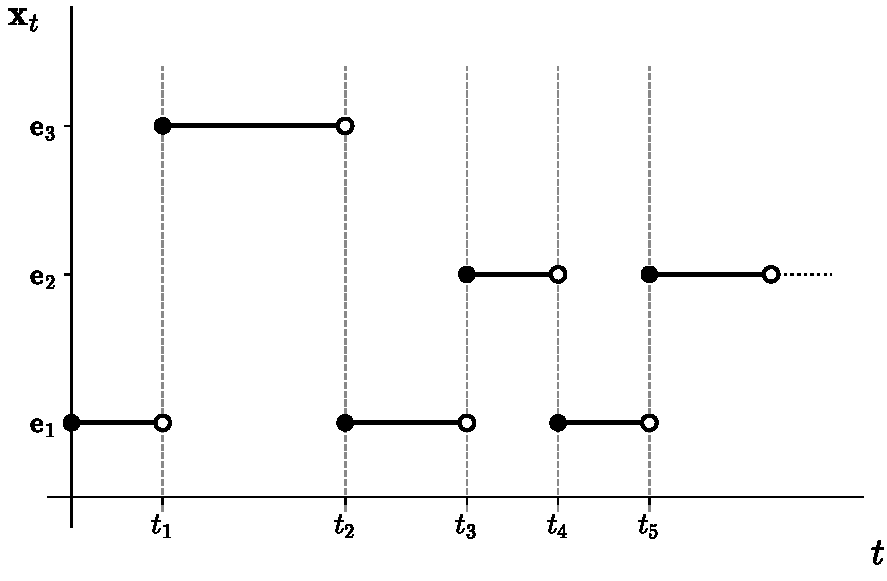
\includegraphics[width=0.8\linewidth]{Images/PartE/ctmc_trajectory.pdf}
    \caption{\textbfs{CTMC 样本路径示意图。}
设状态空间为 $\mathcal{V}=\{\rve_1,\rve_2,\rve_3\}$，在纵轴上标记为 $S_1,S_2,S_3$。
轨迹是分段常值的：过程在 $\rvx_t=\rve_i$ 处停留一段随机的驻留时间，然后在 $t_1,t_2,\ldots$ 等时刻瞬时跳到另一个状态 $\rve_j$。
实心圆圈标记每次跳变后立即占据的状态，空心圆圈标记跳变之前的状态，反映了右连续约定。
虚线段表示超出所显示窗口的延续。
这些跳变时刻和目的地由速率矩阵 $\rmQ_t$ 支配：从状态 $\rve_i$ 出发，过程以瞬时速率 $[\rmQ_t]_{ij}$ 跳到 $\rve_j$（$j\neq i$）。
\figcredit{改编自 \citet{campbell2022continuous}。}}
    \label{fig:ctmc-trajectory}
\end{figure}

\paragraph{无穷小转移。}
在上一小节中，每个转移矩阵 $\rmP_k$ 描述了从时间 $k$ 到时间 $k{+}1$ 的完整一步。现在设想把这些步变得越来越细。令 $\rmP_{t,\Delta t}$ 表示从时间 $t$ 起把系统向前推进一小段时长 $\Delta t$ 的转移矩阵：其元素 $[\rmP_{t,\Delta t}]_{ij}$ 是在区间 $[t,\,t{+}\Delta t]$ 内从状态~$\rve_i$ 转移到状态~$\rve_j$ 的概率。

当 $\Delta t$ 很小时，大部分质量留在原地，只有一小部分发生跳变。这意味着 $\rmP_{t,\Delta t}$ 接近于单位矩阵，可以把它展开为
\begin{equation}
\rmP_{t,\Delta t}
\;=\; \rmI + \rmQ_t\,\Delta t + \mathcal{O}(\Delta t^2),
\label{eq:generator-expansion}
\end{equation}
其中 $\rmQ_t \in \R^{K \times K}$ 是时刻 $t$ 的\emph{速率矩阵}，也称为生成元。如果 $\rmQ_t$ 在时间上足够正则，余项在局部可以写成 $\mathcal{O}(\Delta t^2)$。$\rmQ_t$ 的元素是瞬时
\emph{速率}而非概率。具体而言：
\begin{itemize}[leftmargin=2em]
    \item $[\rmQ_t]_{ij} \geq 0$（$i \neq j$）：这是过程从状态~$\rve_i$ 跳到状态~$\rve_j$ 的速率。乘以 $\Delta t$ 便给出短区间内主导阶的跳变概率。
    \item $[\rmQ_t]_{ii} = -\sum_{j \neq i} [\rmQ_t]_{ij}$：对角元素为负，记录了概率\emph{离开}状态~$\rve_i$ 的总速率。这保证 $\rmQ_t$ 的每一行求和为零，这正是概率守恒在速率层面上的表达。\footnote{这直接来自 $\rmP_{t,\Delta t}$ 的行和约束。由于转移矩阵每一行求和为 $1$，代入展开 $\rmP_{t,\Delta t} = \rmI + \rmQ_t\,\Delta t + o(\Delta t)$ 得到 $1 + \Delta t \sum_{j} [\rmQ_t]_{ij} + o(\Delta t) = 1$，从而迫使 $\sum_{j} [\rmQ_t]_{ij} = 0$。分离出对角项便得 $[\rmQ_t]_{ii} = -\sum_{j \neq i} [\rmQ_t]_{ij}$。}
\end{itemize}
从展开式中读出，在一段短区间内从~$\rve_i$ 跳到 $\rve_j$（$j\neq i$）的概率约为 $[\rmQ_t]_{ij}\,\Delta t$，而留在~$\rve_i$ 的概率约为 $1 - \sum_{j \neq i} [\rmQ_t]_{ij}\,\Delta t$。

\paragraph{主方程。}
有了无穷小转移，连续时间极限便立即得到。把 \Cref{eq:generator-expansion} 中的展开式代入 $\rvp_{t+\Delta t} = \rmP_{t,\Delta t}^\top\,\rvp_t$，并令 $\Delta t \to 0$，得到
\begin{mdframed}
\begin{equation}
\frac{\diff}{\diff t}\,\rvp_t = \rmQ_t^\top\,\rvp_t.
\label{eq:master-equation-vector}
\end{equation}
\end{mdframed}
这是\emph{主方程}，对 CTMC 而言也称为\emph{Kolmogorov 前向方程}~\citep{norris1998markov}。回忆 $\rvp_t$ 是概率向量，其第 $j$ 个分量 $p_t(j)$ 给出在时刻~$t$ 处于状态~$\rve_j$ 的概率。把 \Cref{eq:master-equation-vector} 的第 $j$ 个分量写出来，其含义便很具体：
\begin{equation}
\frac{\diff}{\diff t}\,p_t(j)
= \underbrace{\sum_{i \neq j} p_t(i)\,[\rmQ_t]_{ij}}_{\text{inflow: mass arriving from other states}}
\;-\;
\underbrace{p_t(j)\sum_{\ell \neq j} [\rmQ_t]_{j\ell}}_{\text{outflow: mass departing to other states}}.
\label{eq:master-equation-component}
\end{equation}
$p_t(j)$ 的变化率就是流入减去流出。这就是以微分方程形式表达的概率守恒。

\paragraph{与连续性方程的比较。}
在连续空间中，连续性方程
\[
\partial_t\,p_t(\rvx) + \nabla \cdot
\big(p_t(\rvx)\,\rvv(\rvx,t)\big) = 0
\]
表明密度的变化由速度场 $\rvv$ 之下的概率质量净通量所驱动。主方程用有限状态的语言讲述了同样的事情：$p_t(j)$ 由于速率矩阵 $\rmQ_t$ 所支配的概率净通量而变化。速度场和速率矩阵扮演着类似的结构角色：二者都规定了概率质量如何被重新分配，并且都强制守恒。主要区别是几何上的：在 $\R^D$ 中，质量通过相邻的空间位置流动；在有限状态空间中，质量沿着转移图的允许边跳变。

\begin{figure}[th!]
    \centering
    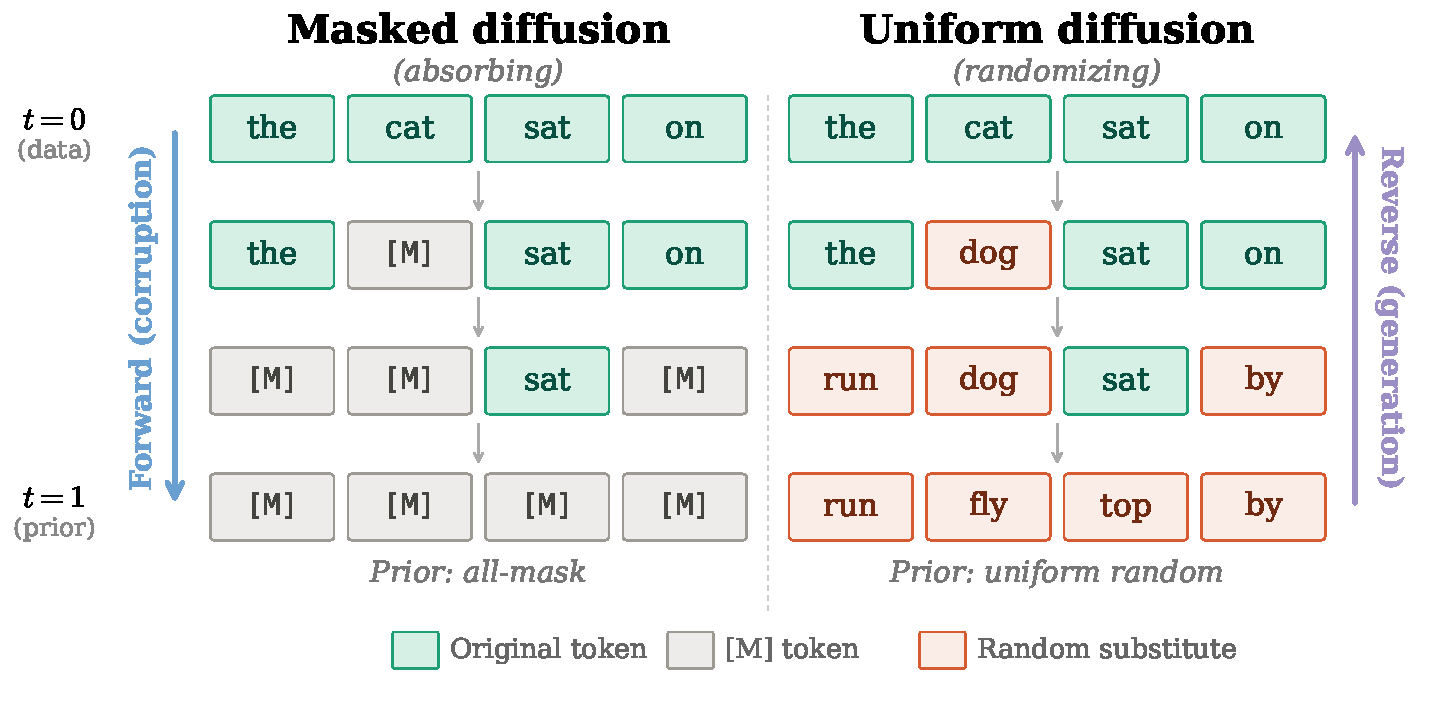
\includegraphics[width=\linewidth]{Images/PartE/masked_vs_uniform_diffusion.pdf}
\caption{\textbfs{掩码扩散与均匀扩散的前向破坏和反向生成示意图。}
这里所示的两个例子都允许形如
$\Pr(\rvx_t|\rvx_0)=\mathrm{Cat}(\rvx_t;\alpha_t\rvx_0+(1-\alpha_t)\bm{\pi})$
的插值边缘分布，其中极限先验 $\bm{\pi}$ 和衰减因子 $\alpha_t$ 由所选的前向速率矩阵决定。在掩码扩散中，词元被吸收到掩码状态，极限先验为 $\bm{\pi}=\rvm=\rve_K$。在均匀扩散中，词元被反复随机化，极限先验为 $\bm{\pi}_{\mathrm{unif}}=\frac{1}{K}\mathbf{1}$。生成过程逆转所选的破坏过程，从对应的简单参考分布出发，或从其有限的有限时间近似出发。
\figcredit{由作者在 AI 辅助编程下绘制。}}
    \label{fig:mask-uniform}
\end{figure}

\paragraph{前向破坏。}
正如连续情形那样，我们需要一个前向过程，逐步破坏数据分布的结构，并将其推向一个易于采样的简单参考分布。这是连续扩散中选择高斯加噪过程的离散类比。设计目标是一致的：破坏应当是渐进的、在解析上或计算上易于处理的，并且足够强，以至于到终止时刻 $T$ 时，数据分布已被基本冲刷掉。

速率矩阵可以有许多选取方式。它可以是均匀的、吸收的、最近邻的、基于图的、化学结构的、语法感知的，或者是为数据领域作其他适配的。下面的两个例子因此并非旨在穷尽分类；它们是让机制变得透明可见的典型情形。
\subparagraph{掩码扩散（吸收式）。} 把最后一个类别保留为掩码词元，记为 $\rvm := \rve_K$。干净数据 $\rvx_0$ 占据前 $K{-}1$ 个类别之一，故 $\langle\rvx_0,\rvm\rangle = 0$。速率矩阵如此定义：每个普通状态以速率 $\beta(t)$ 转移到掩码状态，而掩码状态从不向外转移：
\[
[\rmQ_t]_{iK}=\beta(t),\qquad
[\rmQ_t]_{ii}=-\beta(t),\qquad
[\rmQ_t]_{ij}=0
\quad
\text{for } i<K,\; j\notin\{i,K\},
\]
和
\[
[\rmQ_t]_{Kj}=0
\quad
\text{for all } j.
\]
其想法很简单：每个词元以速率 $\beta(t)$ 独立地被替换为掩码，一旦被掩码便保持掩码。

以干净状态 $\rvx_0$ 为条件的前向边缘分布为
      \[
      \Pr(\rvx_t | \rvx_0)
      = \mathrm{Cat}\bigl(\rvx_t;\;
          \alpha_t\,\rvx_0 + (1-\alpha_t)\,\rvm\bigr),
      \]
      其中
      \[
      \alpha_t
      =
      \exp\left(-\int_0^t\beta(s)\,\diff s\right).
      \]
在时刻~$t$，词元以概率 $\alpha_t$ 等于其干净值 $\rvx_0$，以概率 $1-\alpha_t$ 被掩码。随着时间增长，越来越多的概率质量聚集在掩码状态上。如果 $\int_0^T\beta(s)\diff s$ 很大，那么 $\alpha_T$ 很小，终止分布便接近全掩码的参考分布。

\subparagraph{均匀扩散。} 这一过程不是擦除一个词元，而是逐步将其随机化。一种方便的连续时间归一化方式是让一个词元以相同速率跳到其他 $K-1$ 个状态中的每一个：
      \[
      [\rmQ_t]_{ij} = \frac{\beta(t)}{K - 1}
      \quad\text{for } i \neq j,
      \qquad
      [\rmQ_t]_{ii} = -\beta(t).
      \]
第一个公式说，从状态 $\rve_i$ 出发，词元以相同的瞬时速率跳到每一个备选状态。第二个公式说，离开状态 $\rve_i$ 的总速率为 $\beta(t)$。

前向边缘分布再次取插值形式
      \[
      \Pr(\rvx_t|\rvx_0)
      = \mathrm{Cat} \bigl(\rvx_t;\;
          \alpha_t\,\rvx_0 + (1-\alpha_t)\,\bm{\pi}_{\mathrm{unif}}
        \bigr),
      \]
      其中
      $\bm{\pi}_{\mathrm{unif}}=\tfrac{1}{K}\mathbf{1}\in\R^K$ 是
      均匀概率向量。在上述速率归一化下，
      衰减因子为
      \[
      \alpha_t
      =
      \exp\left(
      -\frac{K}{K-1}\int_0^t \beta(s)\,\diff s
      \right).
      \]
随着时间流逝，反复的随机化会冲刷掉数据分布的结构，把它推向 $\mathcal{V}$ 上的均匀分布。

更一般地，前向过程不必具有简单的混合形式
\[
\Pr(\rvx_t|\rvx_0)
= \mathrm{Cat}\bigl(\rvx_t;\;\alpha_t\rvx_0+(1-\alpha_t)\bm{\pi}\bigr).
\]
那种形式对于直观很有用，也出现在常见的掩码构造和均匀构造中，但马尔可夫定律演化的视角更加一般：转移矩阵支配离散时间演化，速率矩阵通过主方程支配连续时间演化。结构化的离散扩散模型可以使用尊重编辑距离、图邻接、分子有效性、词表结构或其他领域知识的转移规则。在所有情形中，同样的原理都保持不变：前向马尔可夫过程定义一条概率路径，而生成则学习沿该路径反向运动。

\subsection{关于反向建模的三种视角}
\label{subsec:epilogue-three-views}

一旦前向过程及其定律演化就位，剩下的任务与连续情形一致：学习一个反向过程，其边缘分布沿逆向时间回溯前向演化，把简单的参考样本变为数据。在 B 部分，
我们把连续扩散模型组织为三种视角：
变分（\Cref{ch:variational}）、基于分数（\Cref{ch:score-based,ch:score-sde}）和基于流
（\Cref{ch:flow-based}）。同样的三分视角也延续到离散设定中，但有一个重要的提醒：它们并非互斥的学派或固定的论文类别。它们是三种识别``为了逆转概率路径必须学习哪个未知对象''的方式。

\paragraph{变分视角：学习反向转移核。}
在连续情形中（\Cref{sec:ddpm}），变分视角
把扩散视为一个层次化的隐变量模型。前向
过程定义了一条噪声越来越大的隐变量链，目标是
学习能够一次一步地解除破坏的反向转移。真实的反向核 $\Pr(\rvx_{k-1}|\rvx_k)$ 难以处理，因为它依赖于 $\rvx_k$ 的边缘定律，而后者涉及
未知的数据分布。DDPM 的关键洞察是以
干净样本 $\rvx_0$ 为条件：前向后验
$\Pr(\rvx_{k-1}|\rvx_k, \rvx_0)$ 是闭式的高斯分布，而
定理~\ref{thm:equiv-marginal-kl} 表明，针对该
条件后验进行训练，等价于（在不依赖于所学反向模型的项的意义下）针对难以处理的边缘反向核进行训练。于是 ELBO
分解为一系列 KL 项之和（\Cref{eq:ddpm-diffusion}），每个噪声层级一项，每一项都要求所学模型去匹配一个易于处理的
前向后验。

同一套逻辑适用于离散设定。把从数据分布中抽取 $\rvx_0$、再施加固定前向链所得到的联合定律记为 $p$，把学习得到的反向模型记为 $p_{\bphi}$。考虑一条被破坏的 one-hot 状态链
\[
\rvx_0 \;\xrightarrow{\;\rmP_0\;}\; \rvx_1 \;\xrightarrow{\;\rmP_1\;}\;
\cdots \;\xrightarrow{\;\rmP_{L-1}\;}\; \rvx_L,
\]
其中 $\rvx_0$ 从数据分布中抽取，而 $\rvx_L$ 接近一个简单的参考分布，例如全掩码或均匀分布。转移
现在是类别型的而非高斯的，但变分结构是相同的：
\begin{itemize}[leftmargin=2em]
    \item 真实的反向 $p(\rvx_{k-1}|\rvx_k)$ 难以处理，
      因为它依赖于第~$k$ 步的边缘分布。
    \item 以 $\rvx_0$ 为条件，可通过 Bayes 公式使前向后验变得易于处理：
      \[
      p(\rvx_{k-1}|\rvx_k, \rvx_0)
      =
      \frac{p(\rvx_k|\rvx_{k-1})\;p(\rvx_{k-1}|\rvx_0)}
             {p(\rvx_k|\rvx_0)},
      \]
      其中右侧的每个因子都由前向过程决定。
    \item 针对这些条件后验的训练与针对难以处理的边缘反向核的训练具有相同的最佳反向核；二者的差异仅在于一些与 $p_{\bphi}$ 无关的项。
\end{itemize}

示意性地，离散扩散 ELBO 含有如下形式的去噪项
\[
\E_{p(\rvx_{0:L})}
 \Big[
\mathcal{D}_{\mathrm{KL}} \big(
  p(\rvx_{k-1}|\rvx_k, \rvx_0)
  \;\|\;
  p_{\bphi}(\rvx_{k-1}|\rvx_k)
\big)
\Big],
\qquad k=1,\ldots,L.
\]
根据具体模型的不同，完整的 ELBO 还可能包含边界项，例如终止先验项和 $k=0$ 附近的重构项。关键
在于，每个去噪项都要求所学反向核去匹配一个由前向破坏决定的、易于处理的 Bayes 后验。

这里 $p_{\bphi}(\rvx_{k-1}=\rve_i|\rvx_k=\rve_j)$ 表示由神经网络参数化的反向转移概率：给定系统在第~$k$ 步处于状态~$\rve_j$，它给出在第~$k{-}1$ 步来自状态~$\rve_i$ 的概率。对于每个固定的 $\rve_j$，这些值构成关于上一状态的一个类别分布。

与连续 DDPM 的主要形式差别在于，这些 KL 散度是关于离散状态的有限和，而非闭式的高斯表达式。这反映了高斯分布的一个特殊性质：同一变量下两个高斯密度的乘积正比于另一个高斯。在连续 DDPM 中，
前向后验通过高斯因子的相乘来计算，因此结果本身是高斯的，
而 KL 散度简化为只涉及
均值和协方差的简单代数表达式（\Cref{sec:ddpm}）。在离散设定中，
Bayes 公式给出的是类别分布，每个 KL 项都是关于状态的求和。这个和是精确的且在概念上简单，但对于大词表或完整序列空间，它可能需要结构、分解、子采样或专门的参数化。

关于参数化的一个实践要点也值得注意。ELBO 要求所学反向核 $p_{\bphi}(\rvx_{k-1}|\rvx_k)$ 去匹配一个 Bayes 后验，但它并不强制该核的唯一神经参数化。一种常见的选择是干净状态预测，或称 $x_0$-预测
的参数化。精确的边缘反向核满足恒等式
\[
p(\rvx_{k-1}|\rvx_k)
=
\sum_{a}
p(\rvx_{k-1}|\rvx_k,\rvx_0=\rve_a)\,
p(\rvx_0=\rve_a|\rvx_k),
\]
其中求和遍历合法的干净类别。这只是对未知干净状态做边缘化。由于后验 $p(\rvx_0|\rvx_k)$ 依赖于
数据分布，它没有闭式表达。因此，一个模型可以预测一个干净状态分布 $\widehat p_{\bphi}(\rvx_0|\rvx_k)$，并用它来定义
\[
p_{\bphi}(\rvx_{k-1}|\rvx_k)
:=
\sum_{a}
p(\rvx_{k-1}|\rvx_k,\rvx_0=\rve_a)\,
\widehat p_{\bphi}(\rvx_0=\rve_a|\rvx_k).
\]
如果 $\widehat p_{\bphi}(\rvx_0|\rvx_k)$ 等于真实后验
$p(\rvx_0|\rvx_k)$，这个混合便能恢复精确的反向核。在
实践中，这是把所学反向转移与已知的前向后验联系起来的有用方式。

这种干净状态参数化在多项式/D3PM 式
离散时间扩散模型~\citep{hoogeboom2021argmax,austin2021structured} 中很常见，但它并不是离散扩散的定义。D3PM 本身就指出，可以直接预测反向 logits，而后续模型则使用为前向过程量身定制的其他结构化参数化
\citep{sahoo2024simple}。因此，干净状态预测应被视为变分视角下的一种重要参数化，而非建模反向过程的唯一方式。

\paragraph{分数/比率视角：学习局部概率比较。}
在连续情形中（\Cref{ch:score-based,ch:score-sde}），基于分数的视角从一个简单的问题出发：给定一个被破坏的样本 $\rvx_t \sim p_t$，要逆转扩散，需要关于当前密度的什么局部信息？答案是分数函数
$\nabla_{\rvx}\log p_t(\rvx)$，它出现在逆向时间
SDE 和概率流 ODE\@。因此，用神经网络学习分数便足以完成生成。

在有限状态空间中，没有周围的欧几里得几何，没有普通的无穷小位移概念，也没有关于状态的梯度。一个样本不会
通过取一个小的欧几里得步长来运动，而是通过从一个状态跳到另一个状态来改变。
因此分数 $\nabla_{\rvx}\log p_t(\rvx)$ 没有直接的、字面上的类比。但
反向过程仍必须回答一个类似的问题：\emph{如果
系统当前处于状态~$\rve_j$，那么每个候选源状态~$\rve_i$ 相对于它有多可能？}

\subparagraph{推导反向跳变速率。}
为了识别所需的量，考虑一个具有速率矩阵~$\rmQ_t$ 和边缘 $\rvp_t$ 的前向 CTMC $\{\rvx_t\}_{0\leq t\leq T}$。元素 $[\rmQ_t]_{ij}$ 是从
状态~$\rve_i$ 到状态~$\rve_j$ 的跳变速率。在一段短区间~$\Delta t$ 内，
无穷小前向事件
$\rvx_t=\rve_i$ 且 $\rvx_{t+\Delta t}=\rve_j$（$i\neq j$）的概率约为
\[
p_t(i)\,[\rmQ_t]_{ij}\,\Delta t.
\]

现在定义反向时间过程 $\bar{\rvx}_s := \rvx_{T-s}$（$0\leq s\leq T$）。它在反向时间 $s$ 处的边缘为 $\bar{\rvp}_s=\rvp_{T-s}$。如果反向过程具有速率矩阵 $\bar{\rmQ}_s$，那么从 $\rve_j$ 到 $\rve_i$ 的相应反向跳变必须在逆序的时间顺序下重现相同的无穷小路径概率。取极限 $\Delta t\to 0$，得到非对角的时间反演公式
\begin{mdframed}
\begin{equation}
[\bar{\rmQ}_s]_{ji}
= [\rmQ_{T-s}]_{ij}\;\frac{p_{T-s}(i)}{p_{T-s}(j)},
\qquad i \neq j,
\label{eq:reverse-rate-discrete-reverse-time}
\end{equation}
\end{mdframed}
只要 $p_{T-s}(j)>0$。等价地，若 $t$ 表示相应的前向时间，而 $\widetilde{\rmQ}_t$ 表示按该前向时间索引的反向生成元，则有
\begin{equation}
[\widetilde{\rmQ}_t]_{ji}
= [\rmQ_t]_{ij}\;\frac{p_t(i)}{p_t(j)},
\qquad i \neq j.
\label{eq:reverse-rate-discrete}
\end{equation}
对角元素由行和为零的约束所确定，
\[
[\widetilde{\rmQ}_t]_{jj}
=
-\sum_{i\neq j}[\widetilde{\rmQ}_t]_{ji}.
\]
这是 CTMC 的标准时间反演公式
\citep{kelly1979reversibility,anderson2012continuous}，由 \citet{campbell2022continuous} 应用于离散扩散。该公式仅在具有正边缘概率的状态上有意义。此外，
反向过程只沿着前向过程所允许的转移逆转概率通量：如果 $[\rmQ_t]_{ij}=0$，那么从 $\rve_j$ 到 $\rve_i$ 的相应反向速率也为零。该陈述并非一种平衡的细致平衡假设；它是关于无穷小路径概率的局部时间反演恒等式。

\subparagraph{比率作为分数的离散类比。}
现在审视 \Cref{eq:reverse-rate-discrete}。前向速率
$[\rmQ_t]_{ij}$ 是已知的，因为前向过程由设计固定。
未知的量是比率 $p_t(i)/p_t(j)$，
它在当前边缘下比较状态~$\rve_i$ 相对于
状态~$\rve_j$ 有多可能。用内积记号，
$p_t(i) = \langle\rvp_t,\rve_i\rangle$，所以该比率可以写成
$\langle\rvp_t,\rve_i\rangle / \langle\rvp_t,\rve_j\rangle$。

为什么这是分数的离散类比？在连续空间中，
分数 $\nabla_{\rvx}\log p_t(\rvx)$ 度量的是
在一个无穷小位移之下对数密度的变化。在有限状态空间中，
自然的局部比较则跨越一个从一个状态
到另一个状态的允许跳变。沿着从~$\rve_j$ 到~$\rve_i$ 的跳变，对数概率的变化为
\[
\log p_t(i) - \log p_t(j)
= \log \frac{p_t(i)}{p_t(j)},
\]
这是对数概率的有限差分，扮演着
$\log p_t$ 的方向导数在~$\R^D$ 中所扮演的角色。这种比较自然是\emph{边局部的}：该比率只在由前向跳变结构所连接的状态对上才需要。因此，离散分数并不是 $\mathbb{R}^D$ 上的欧几里得向量场；它是沿着允许转移的一系列局部概率比较。对于完整序列，同样的陈述在把 $i$ 和 $j$ 替换为完整构型（通常是 Hamming 型或基于图的转移结构下的相邻构型）后依然成立。

\subparagraph{网络学习什么。}
在连续基于分数的模型中，训练一个神经网络
$\rvs_{\bm{\phi}}(\rvx, t)$ 来逼近分数
$\nabla_{\rvx}\log p_t(\rvx)$，并把所学分数代入
逆向时间 SDE 来生成样本。离散情形在信息层面上遵循同一逻辑：网络必须提供为通过
\Cref{eq:reverse-rate-discrete} 确定反向跳变速率所需的、随时间变化的比率信息。随后，生成通过使用所学转移概率或速率来模拟逆向时间马尔可夫链或 CTMC 进行。

不同的表述以不同方式表示这一信息。基于比率的模型，如 SEDD~\citep{lou2024discrete}
，使用受分数匹配启发的损失来估计比率 $p_t(i)/p_t(j)$ 或其对数形式。其他连续时间表述
\citep{campbell2022continuous,sun2023scorebased} 则通过诸如匹配条件转移概率的目标来学习等价的反向量。把局部概率比较视为分数的离散类比这一想法
由 \citet{meng2022concrete} 的\emph{具体分数}（concrete score）所形式化。
尽管在参数化上有这些差异，底层原理
是共通的：学习时间反演所需的局部概率比较，构造反向转移或速率，并向后模拟。

\paragraph{流视角：学习一个离散传输场。}
在连续情形中（\Cref{ch:flow-based}），基于流的视角
采取的是另一条路径：与其先学分数再逆转
SDE，不如直接学习一个速度场 $\rvv_t(\rvx)$，其 ODE 流
把参考分布传输到数据分布。其
训练策略是流匹配
（\Cref{sec:flow-matching-framework}）：边缘速度场是难以处理的，但一个\emph{条件}速度场
$\rvv_t(\rvx | \rvx_0)$，以数据样本或端点样本为条件，有闭式表达。边缘目标与条件目标通过下式联系：
\[
\rvv_t(\rvx)
= \E \big[\rvv_t(\rvx | \rvx_0) | \rvx_t = \rvx\big],
\]
这是在给定当前状态下对所有可能条件变量的平均。显式计算这一平均需要知道连续边缘
密度 $p_t(\rvx)$。关键的训练技巧（\Cref{subsec:fm-instantiations}）在于，
在平方误差回归下，条件目标与难以处理的边缘目标具有相同的总体最小化子。因此，训练通过使用来自易于处理的条件路径的样本来避开显式的边缘计算。

离散情形遵循同样的想法，只是用速率矩阵替代速度场。由于离散状态无法
沿词元空间中的连续轨迹运动，速度场的角色由一个速率矩阵（也称为马尔可夫生成元）$\rmQ_t$ 来扮演。回忆元素 $[\rmQ_t]_{ij}$ 规定了从状态~$\rve_i$ 到状态~$\rve_j$ 的跳变速率；单位时间内从~$\rve_i$ 实际送到~$\rve_j$ 的概率质量是通量
\[
J_t(i,j)=p_t(i)\,[\rmQ_t]_{ij}.
\]
在这个意义上，速率矩阵是一个离散的传输场：它决定了概率质量如何随时间被重新分配。

这里有一个重要的微妙之处。一条概率路径 $\{\rvp_t\}_{t\in[0,T]}$ 并不唯一地确定一个速率矩阵。许多不同的生成元都可以在主方程中产生相同的导数 $\diff\rvp_t/\diff t$，正如不同的传输场有时也能在不同的几何约束下实现相同的边缘演化。因此，一个离散流匹配方法不仅指定一条概率路径，还要指定一条沿该路径赋予条件跳变速率或概率流的规则。

正如连续流匹配那样，边缘速率矩阵通常是难以处理的，但条件版本往往可以显式给出。如果
以一个端点（例如干净数据状态和/或参考状态）为条件，就可以规定一条条件概率路径，并沿该路径导出易于处理的条件跳变速率。随后，在适当的恰当损失下训练一个神经网络，从被破坏的样本预测相应的转移或速率信息。边缘生成元通过同样的条件期望原理得到：在给定当前状态下对未知端点分布求该条件传输对象的平均，但该平均是通过对条件目标的监督回归或分类来学习，而非显式计算。

与连续流匹配的对应关系如下：
\begin{itemize}[leftmargin=2em]
    \item 在连续流匹配中，网络学习一个条件
      速度场；边缘速度作为流匹配损失下的最佳预测子而涌现。
    \item 在离散流匹配中，网络学习条件
      转移或跳变速率信息；边缘离散传输场通过类似的条件期望机制而涌现。
\end{itemize}
在两种情形中，训练都通过使用易于处理的条件路径和采样的中间状态，来避开难以处理的边缘定律。

这一视角由 \citet{campbell2024generative} 和
\citet{gat2024discrete} 在离散流模型或离散流匹配的名目下发展。更广义地说，流视角应被理解为关于\emph{学习的是什么对象}的陈述：离散状态空间上的一个传输场，由转移、速率或概率流来表示。

\subsection{何者相似，何者真正不同？}
\label{subsec:epilogue-genuine-diff}

下表总结了连续扩散模型与离散扩散模型之间的对应关系。横向阅读每一行，可以看到同一概念成分在两种不同设定下的实例化：

\begin{table}[!t]
\caption{\textbfs{概率传输的连续视角与离散视角。}
同样的生成式建模成分既出现在连续状态空间中，也出现在有限离散状态空间中，但数学对象发生了变化：密度变成概率向量，ODE/SDE 动力学变成马尔可夫链或 CTMC，而反向建模则通过转移核、分数/比率信息或离散传输场来表达。}
\label{tb:continuous-discrete-diffusion}
\centering
\begingroup
\scriptsize
\setlength{\tabcolsep}{4pt}
\renewcommand{\arraystretch}{1.08}
\begin{tabular}{p{0.15\linewidth} p{0.40\linewidth} p{0.40\linewidth}}
\toprule
\textbfs{状态}
& \textbfs{连续} $(\rvx \in \R^D)$
& \textbfs{离散} $(\rvx \in \mathcal{V} \subset \{0,1\}^K)$ \\
\midrule

\textbfs{定律}
& 密度 $p_t(\rvx)$
& 概率向量 $\rvp_t \in \Delta^{K-1}$ \\
\graymidrule

\textbfs{样本 \newline 动力学}
& ODE 或 SDE 轨迹
& 马尔可夫链或 CTMC 跳变 \\
\graymidrule

\textbfs{定律 \newline 演化}
& 连续性方程或 Fokker--Planck 方程
& 转移矩阵传播或主方程 \\
\graymidrule

\textbfs{传输 \newline 对象}
& 速度场、漂移、扩散或分数场
& 转移核、速率矩阵、比率或概率流 \\
\graymidrule

\textbfs{参考 \newline 定律}
& 简单分布，例如高斯
& 简单分布，例如均匀或全掩码 \\

\midrule
\multicolumn{3}{c}{\textbfs{反向建模的三种视角}} \\
\midrule

\textbfs{变分}
& 带有高斯或连续转移的 ELBO
& 带有类别型转移的 ELBO \\
\graymidrule

\textbfs{分数/比率}
& 学习分数 $\nabla_{\rvx}\log p_t(\rvx)$
& 学习比率或对数比率，例如 $p_t(i)/p_t(j)$ \\
\graymidrule

\textbfs{流}
& 学习速度场 $\rvv_t(\rvx)$
& 学习转移、速率或流场 \\

\bottomrule
\end{tabular}
\endgroup
\end{table}
\noindent
这种对应关系很干净，但离散设定
并不仅仅是把连续理论中的梯度替换为比率。有几个更深层的差异值得强调。

\paragraph{没有字面意义上的逆映射。}
在一个确定性连续归一化流中，反向映射就是前向映射的字面意义上的逆。而在离散马尔可夫过程中，前向核可能会合并来自多个状态的质量，因而不必可逆。因此，反向过程不是通过矩阵求逆得到的。它是一种依赖于当前边缘定律的 Bayes 或时间反演构造。这就是反向转移概率中含有诸如 $p_k(i)/p_{k+1}(j)$ 的因子、反向跳变速率中含有诸如 $p_t(i)/p_t(j)$ 的比率的原因。

\paragraph{几何与样本路径。}
在连续欧几里得空间中，单个样本沿
连续时间轨迹演化：ODE 解是光滑的，而 SDE 样本
路径是连续的，尽管通常处处
不可微。这种微分结构使得速度场、分数函数和散度等对象有意义。相比之下，在有限状态空间中，单条轨迹是
\emph{纯跳变路径}：它在一个状态上停留一段随机的驻留时间，然后突然跳到另一个状态。平滑演化的不是样本路径本身，而是概率向量 $\rvp_t$，它按主方程在概率单纯形上随时间连续演化。因此，离散扩散仍然在概率演化的层面上允许一种统一的描述，但其样本层面的动力学由跳变过程支配，而非由数据空间中的连续 ODE/SDE 路径支配。

\paragraph{前向破坏结构与反向参数化。}
在离散扩散中，前向破坏过程往往是一个实质性的建模选择。在连续高斯扩散中，人们可以调整调度 $\alpha_t$ 和 $\sigma_t$，但前向核通常仍是高斯的，因此主要作用是控制破坏的速率与尺度。相比之下，在离散扩散中，转移规则本身可以改变：可以使用均匀破坏、掩码、最近邻转移、图结构转移、领域专用转移，或更一般的概率路径。正如 D3PM~\citep{austin2021structured} 所强调的，前向过程因此可以直接纳入领域专用的归纳偏置，而这反过来又塑造了反向生成问题。

这一差异也改变了反向参数化的地位。在高斯设定中，噪声、去噪数据、分数和速度等常见目标由简单的随时间变化的仿射变换联系在一起。在离散设定中，反向转移概率、干净状态预测子、概率比率和跳变速率则通过归一化、Bayes 公式以及所选的转移图联系在一起。它们相互关联，但不仅仅是可互换的高斯式重参数化。因此，变分、分数/比率和流的描述是反向问题的真正不同的视角，而不仅仅是同一代数目标的不同名称。

\paragraph{采样机制。}
采样过程也不同。在连续扩散中，生成通常通过在选定的时间网格上数值积分 ODE 或 SDE 来实现。在离散扩散中，生成意味着模拟一条反向马尔可夫链或 CTMC\@。在离散时间下，这等价于采样类别型反向转移。在连续时间下，它可能涉及从所学速率模拟跳变，例如通过事件驱动模拟或时间离散化。因此，连续扩散中由数值 ODE/SDE 求解器所扮演的角色，在离散设定中被类别型转移采样或跳变过程模拟所取代。

\paragraph{为何止步于此？}
本节的目标并不是要发展离散扩散模型的完整机制，而是要识别出在不同状态空间之间保持不变的那个原理。关键之处是结构性的：在连续空间中，分布演化由变量替换原理及其微分形式（包括连续性方程和 Fokker--Planck 方程）支配。在离散空间中，相应的角色由马尔可夫算子和主方程扮演。在两种设定中，建模逻辑都是相同的：定义一个前向破坏过程，理解它如何传输分布，然后为生成学习一个反向传输机制。这一逻辑并不取决于底层状态空间是连续的还是离散的。

发生变化的，是用来实现这一纲领的数学对象，而不是纲领本身。在连续空间中，人们处理的是密度、梯度、速度场和 SDE 或 ODE 动力学。在离散空间中，人们处理的是概率向量、转移核、跳变速率、比率和概率流。这些差异在技术上是重要的，并引出关于参数化、训练和采样的不同问题。但它们并不改变更深层的结论：概率传输的视角并不绑定于某个特定的状态空间、架构或论文谱系。它是一种足够一般的组织原理，足以在一个统一的概念框架内同时容纳连续扩散与离散扩散。

\clearpage
\newpage

\section{全书结语}\label{sec:epilogue-closing}
扩散模型乍看之下也许像是一堆缩写、参数化和算法变体的集合。然而其核心思想很简单。它们提供了一种通过规定概率律如何随时间演化来构造生成器的方式。从这个视角看，生成并不是一个神秘的黑箱，而是粒子云在前向过程及其所学反向之下的受控传输。

在全书之中，这一视角以多种形式出现。在连续状态空间中，变分、基于分数和基于流的表述提供了描述和学习一个预设定律演化之反向的不同方式。受扩散启发的快速生成器，例如流映射模型，也属于同一故事：它们并不放弃传输视角，而是追问底层的生成动力学能否被更直接地表示、更高效地执行。在离散状态空间中，同样的结构思想以马尔可夫核、跳变过程、比率和主方程的语言再次出现。

因此，本书的主要信息并不是某一种特定的表述应当取代所有其他表述。相反，扩散最好被理解为从预设前向过程构造生成器的一般原理~\citep{lai2026unified}。在这一视角下，不同的状态空间自然引出不同的反向表示。在连续设定中，人们可以处理条件高斯、分数函数、速度场或更直接的流映射。在离散设定中，人们可以处理反向转移概率、干净状态预测子、概率比率、跳变速率，或与底层马尔可夫过程相关联的概率流。重要的不是参数化的标签，而是前向过程、概率律的诱导演化以及所学生成机制能否连贯地契合在一起。

我们希望本书已经把这一结构讲清楚：一个前向过程诱导出概率律的演化，而生成式建模无非是学习如何逆转、近似或利用这一演化。具体方法将继续变化，但这一视角为理解它们为何有效、如何相互关联，以及新的发展可能从何而来，提供了一个稳定的立足点。

\epigraph{\textit{重要的是不要停止提问。好奇心自有其存在的理由。}}{Albert Einstein}

% \part{Postface}
% \input{9_Postface and Conclusion}

%%%%%%%%%%%%%%%%%%%%%%%%%%%%%%%%%%%
%%%%%%%%%%%%%%%%%%%%%%%%%%%%%%%%%%%



\appendix

\chapter{微分方程速成}\label{app:de}

微分方程（DE）是对动态系统进行建模的基本工具，大体上可以分为\emph{常微分方程}（ODE）、\emph{随机微分方程}（SDE）和\emph{偏微分方程}（PDE）三类。

常微分方程描述了一个系统的状态如何按照某种精确的规则随时间变化，因此只要知道起点，就能完全确定其未来的轨迹。随机微分方程在这种演化过程中引入了随机性，用以刻画噪声或不确定性对系统行为的影响，使得结果不再是确定性的，而是具有概率性质。偏微分方程则解释了依赖于多个变量（例如时间和空间）的函数如何共同演化，能够描述诸如热量扩散、波动传播，以及\emph{随机系统中概率密度的时间演化}等现象（剧透：Fokker-Planck 方程）。这些类型的微分方程构成了一种基础语言，用于理解系统在确定性影响与随机性影响下如何随时间和空间演化。

在本章中，我们将介绍微分方程方面的必备预备知识。

\clearpage
\newpage

\section{常微分方程基础}

本节介绍常微分方程的基本理论，着重强调在给定初始条件下解的唯一性。同时，本节还涵盖了使用数值求解器求解常微分方程的实用方法。


\subsection{常微分方程的直观理解}

确定性的过程被称为\emph{常微分方程}（ODE）。在多变量的情形下，我们考虑如下形式的方程组：
\begin{equation}\label{eq:general_ode}
    \frac{\diff \mathbf{x}(t)}{\diff t} = \mathbf{v}(\mathbf{x}(t), t),
\end{equation}
其中 $\mathbf{x}(t) \in \mathbb{R}^D$ 是一个向量值函数，表示系统在时刻 $t$ 的状态；而 $\mathbf{v}: \mathbb{R}^D \times \mathbb{R} \to \mathbb{R}^D$ 是一个向量场，规定了空间和时间内每一点处变化的方向与大小。


\paragraph{求解常微分方程的高层直观。}
\begin{figure}[th]
    \centering
    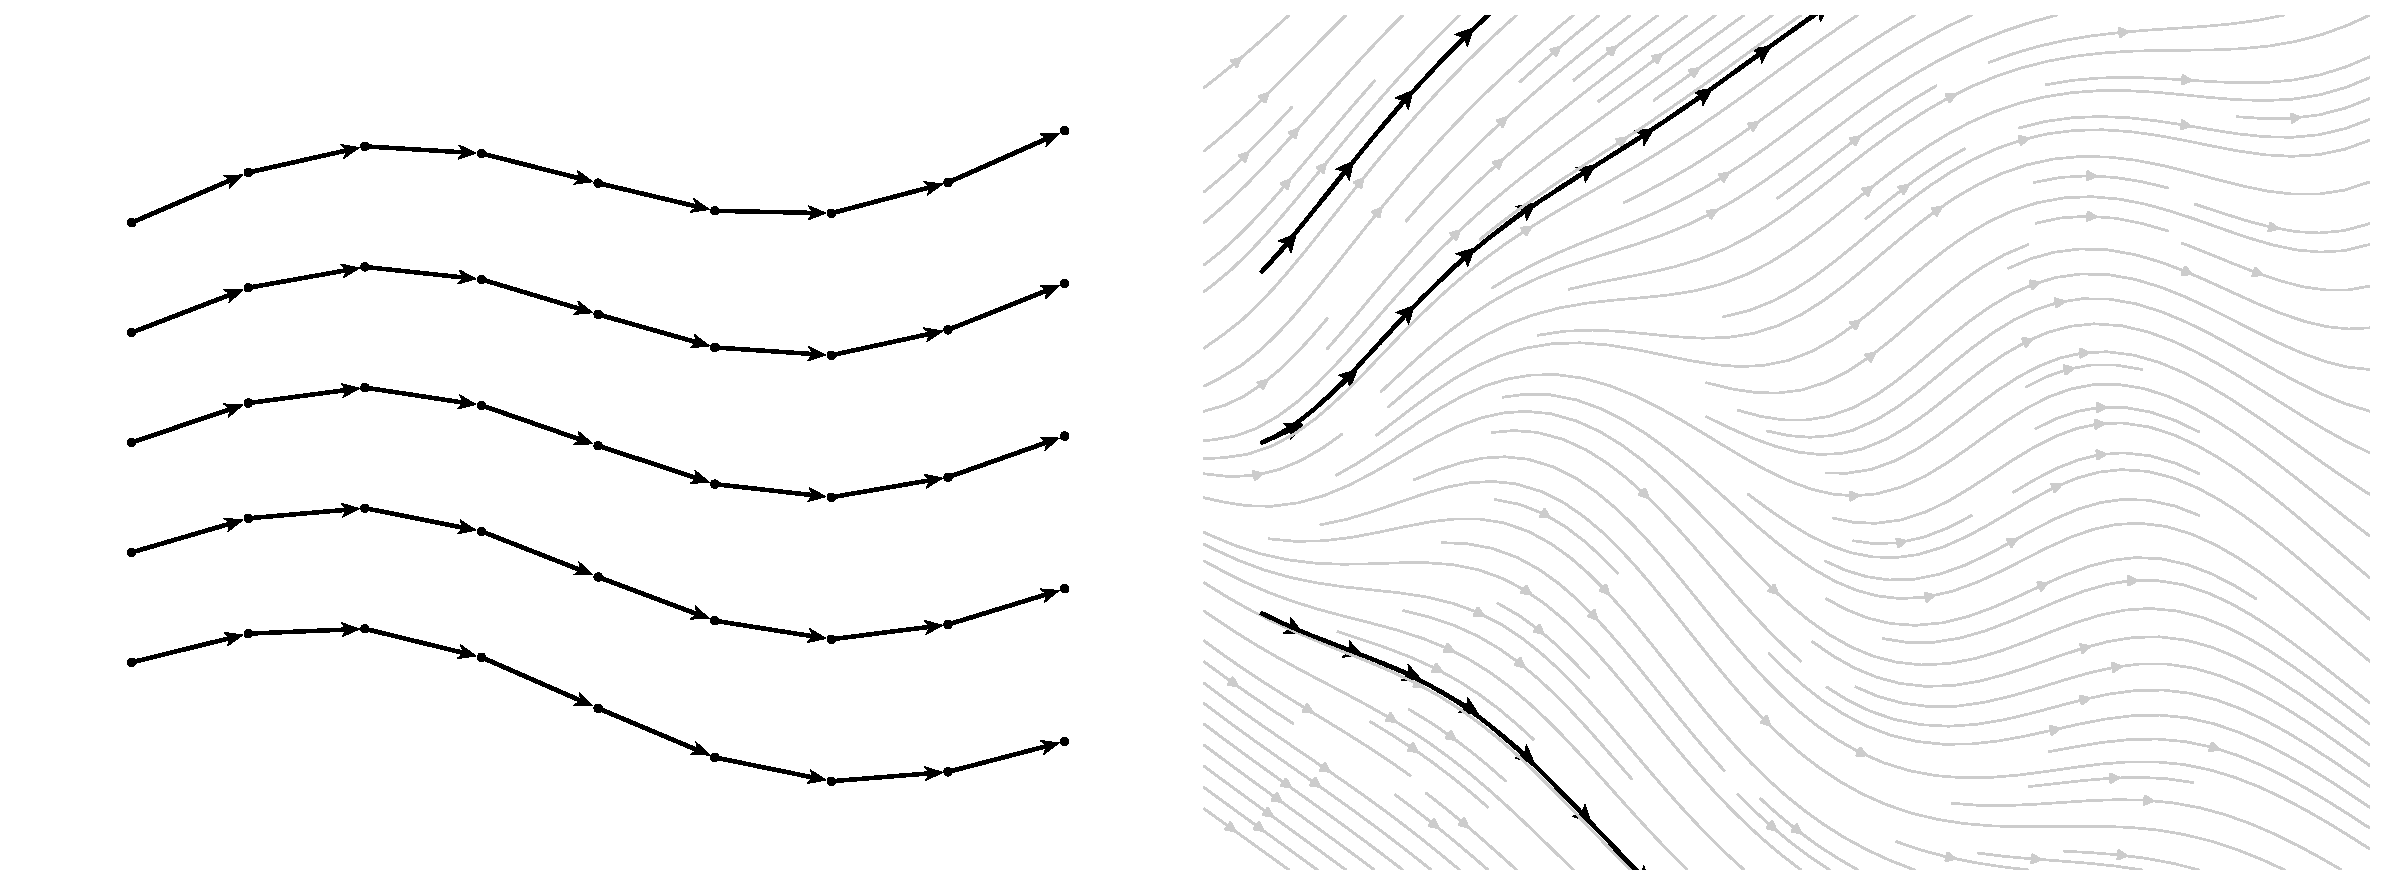
\includegraphics[width=\linewidth]{Images/PartE/discrete_vs_continuous_ode.pdf}
    \caption{\textbfs{常微分方程示意图。}
速度场 $\rvv(\rvx,t)$ 在每一点处都赋予一个漂移向量。
解轨迹 $\rvx(t)$ 是一条路径，其切线方向始终与局部漂移方向一致。
左图展示了逐步推进的求解器更新（点与箭头），用以近似该路径；
右图则展示了与速度场保持一致流动的精确轨迹（黑色）。在未指定初始状态 $\rvx(0)$ 的情况下，存在无穷多条瞬时变化与同一速度场相匹配的轨迹。
然而一旦 $\rvx(0)$ 被固定，常微分方程便唯一确定一条依照漂移方向流动的路径 $\rvx(t)$。
\figcredit{由作者绘制。}}
    \label{fig:ode-illustration}
\end{figure}

为了建立直观理解，可以将向量场 $\mathbf{v}(\mathbf{x}, t)$ 想象成一幅动态的箭头地图，它告诉你一个点 $\mathbf{x}$ 在任意给定时刻 $t$ 应当如何运动。求解这个微分方程，意味着要在这个场中描绘出一条曲线 $\mathbf{x}(t)$，使得该曲线在任一点的切线（即瞬时速度）都与 $\mathbf{v}(\mathbf{x}(t), t)$ 所给出的向量方向一致。
\begin{itemize}
    \item \textbfs{向量场视角：} 函数 $\mathbf{v}(\mathbf{x}, t)$ 定义了事物应当如何运动：它给出了关于运动或变化的局部"指令"。
    \item \textbfs{轨迹视角：} 解 $\mathbf{x}(t)$ 是一条路径，若一个粒子在每一瞬时都遵循由向量场 $\mathbf{v}$ 所设定的规则，它便会沿着这条路径运动。
\end{itemize}
因此，求解一个常微分方程就好比将一个粒子放入流场之中，并观察它随时间的运动方向。

\subsection{常微分方程的存在性与唯一性}
到目前为止，我们已经看到，求解一个常微分方程意味着寻找一条在每一点处都遵循向量场所给方向的路径。直观地讲，这就像是追踪一个粒子沿着由速度所定义的流运动时的轨迹。

但这种图景引出了一个重要的问题：
\begin{question}
    如果我们选定一个起点，能否确信确实存在一条遵循这些方向的路径？如果存在，那么这条路径是唯一的吗，还是粒子有可能突然跳到另一条不同的轨迹上？
\end{question}

回答这些问题至关重要，因为它告诉我们系统的行为能否从其起始位置被可靠地预测。
\emph{存在性与唯一性定理}给出了向量场应满足的条件，这些条件能够保证从任意给定的初始点出发恰好存在一条路径。
这确保了解的行为是一致的，并构成了常微分方程理论的基石。


\paragraph{局部（时间上）的存在性与唯一性定理。}


下面，我们陈述该定理的一个\emph{局部}版本，它断言在给定初始条件下，在初始时刻的某个邻域内解的存在性与唯一性。

\thmp{局部存在性与唯一性}{ode-local}{
设 $\mathbf{v}(\mathbf{x}, t)$ 是关于 $\mathbf{x}$ 和 $t$ 在区域 $D \subseteq \mathbb{R}^D \times \mathbb{R}$ 上的连续函数。如果 $\mathbf{v}$ 关于 $\mathbf{x}$ 满足 Lipschitz 条件：
\[
\|\mathbf{v}(\mathbf{x}_1, t) - \mathbf{v}(\mathbf{x}_2, t)\| \leq L \|\mathbf{x}_1 - \mathbf{x}_2\| \quad \forall (\mathbf{x}_1, t), (\mathbf{x}_2, t) \in D,
\]
其中 $L > 0$ 是常数，那么对于每一个初始条件 $\mathbf{x}(t_0) = \mathbf{x}_0$，都存在唯一的解 $\mathbf{x}(t)$ 在某个区间 $[t_0 - \delta, t_0 + \delta]$ 上满足 \Cref{eq:general_ode}。}{（证明思路）存在性与唯一性定理可以借助 Picard-Lindel\"of 迭代方法进行构造性地证明。该方法生成一个函数序列 $\{\mathbf{x}_n(t)\}$，该序列收敛到解 $\mathbf{x}(t)$。迭代定义为：
\[
\mathbf{x}_{n+1}(t) = \mathbf{x}_0 + \int_{t_0}^t \mathbf{v}(\mathbf{x}_n(s), s) \diff s.
\]
\begin{itemize}
    \item 从一个初始猜测 $\mathbf{x}_0(t) = \mathbf{x}_0$ 出发。
    \item 利用上述积分形式迭代地精化 $\mathbf{x}_n(t)$。
    \item 在 Lipschitz 条件下，通过应用压缩映射原理可保证收敛性。
\end{itemize}
}
该证明的本质根植于 Picard–Lindelöf 迭代方法，其核心思想也在 \Cref{sec:picard} 中被用于加速扩散模型的采样过程。


\paragraph{全局（时间上）的存在性与唯一性定理。}
局部存在性与唯一性定理保证了解在一个小时间区间上的存在性，而"全局（时间上）存在性与唯一性定理"则在附加的正则性条件下将此结果推广到整个区间 $[t_0, T]$。此类中一个著名的结果是 \emph{Carathéodory 定理}，它在两个关键假设下保证常微分方程解的全局存在性与唯一性：状态变量的局部 Lipschitz 连续性，以及线性增长界。

\begin{enumerate}[label=(\roman*)]
    \item \textbfs{关于 $\mathbf{x}$ 的局部 Lipschitz 条件：} 存在一个在 $[0, T]$ 上可积的函数 $\mathrm{Lip}(t)$，使得对所有的 $\mathbf{x}_1, \mathbf{x}_2 \in \mathbb{R}^D$，
    \[
    \|\rvv(\mathbf{x}_1, t) - \rvv(\mathbf{x}_2, t)\| \leq \mathrm{Lip}(t) \|\mathbf{x}_1 - \mathbf{x}_2\|.
    \]

    \item \textbfs{线性增长条件：} 存在一个在 $[0, T]$ 上可积的函数 $M(t)$，使得对所有的 $\mathbf{x} \in \mathbb{R}^D$，
    \[
    \|\rvv(\mathbf{x}, t)\| \leq M(t)(1 + \|\mathbf{x}\|).
    \]
\end{enumerate}
关于这些假设、定理的严格表述及详细证明，我们建议读者参阅 \citep{reid1971ordinary}。

\rmkb{要将这些定理应用于扩散模型中的概率流常微分方程（参见 \Cref{eq:prob_ode_gt}），可能需要对分数函数 $\nabla_\rvx \log p_t(\rvx)$ 施加额外的假设，例如条件 (i) 和 (ii)。对于不关注技术细节的读者而言，这些假设可以合理地直接接受，而无需进一步的论证。
}

总而言之，当给定的初始条件被赋予一个由含时速度场定义的常微分方程时，粒子流动的轨迹便被唯一地确定。

\paragraph{唯一性蕴含解的不相交性} 正如局部存在性与唯一性定理所保证的那样，常微分方程解的唯一性蕴含了一个基本性质：从不同初始条件出发的两条不同的解轨迹不可能相互交叉。这反映了常微分方程的确定性本质，确保每一个状态都沿着一条唯一的路径演化。下面的推论将这一结果形式化。


\corp{解的不相交性}{
考虑常微分方程的两个解 $\rvx_1(t)$ 和 $\rvx_2(t)$
\[
\frac{\diff \rvx(t)}{\diff t} = \rvv\left(\rvx(t),t\right), \quad t \in [0,T].
\]
假设它们具有不同的初始值 $\rvx_1(0) \neq \rvx_2(0)$。那么这两个解在 $[0,T]$ 上不相交，即
\[
\rvx_1(t) \neq \rvx_2(t) \quad \text{for all } t \in [0,T].
\]
}{反证，假设存在某个 $t^* \in (0,T]$ 使得
\[
\mathbf{x}_1(t^*) = \mathbf{x}_2(t^*).
\]
定义两个解首次相遇的时刻为
\[
t_0 := \inf \{ t \in [0,T]|\mathbf{x}_1(t) = \mathbf{x}_2(t) \}.
\]
由于 $\mathbf{x}_1(0) \neq \mathbf{x}_2(0)$ 且 $t^*$ 属于该集合，因此有 $t_0 > 0$。由 $\mathbf{x}_1$ 和 $\mathbf{x}_2$ 的连续性可得
\[
\mathbf{x}_1(t_0) = \mathbf{x}_2(t_0).
\]

考虑初值问题
\[
\frac{\mathrm{d}\mathbf{x}(t)}{\mathrm{d}t} = \mathbf{v}(\mathbf{x}(t), t), \quad \mathbf{x}(t_0) = \mathbf{x}_1(t_0).
\]
由常微分方程的唯一性定理，$\mathbf{x}_1$ 和 $\mathbf{x}_2$ 必须在区间 $[t_0, T]$ 上一致。对时间反向应用唯一性同样意味着这两个解在 $[0, t_0]$ 上也一致。
因此，这两个解满足
\[
\mathbf{x}_1(t) = \mathbf{x}_2(t) \quad \text{for all } t \in [0, T],
\]
这与 $\mathbf{x}_1(0) \neq \mathbf{x}_2(0)$ 的假设相矛盾。由此我们得出结论
\[
\mathbf{x}_1(t) \neq \mathbf{x}_2(t) \quad \text{for all } t \in [0, T].
\]

}

通过保证解的路径不相交，该定理为流映射模型提供了隐含却至关重要的支撑（参见 \Cref{ch:distillation,ch:fast-scratch}）。



\subsection{指数积分因子}\label{app:exp-int-factor}
即使是由一般含时速度 $\rvv$ 所确定的常微分方程也无法得到闭式解，但在某些特殊情形下，我们可以解析地求解它们，或者将其形式归约为一个具有更好结构的形式。
\paragraph{一个示例。}
考虑如下的线性标量常微分方程：
\[
\frac{\diff \rvx(t)}{\diff t} = L(t)\rvx(t),
\]
其中 $L(t) \in \mathbb{R}$ 是连续函数。该方程可求得闭式解，其解广为人知（对任意 $s$ 和 $t$）：
\[
\rvx(t) = \rvx(s) \cdot \exp\left( \int_s^t L(\tau) \,\diff \tau \right).
\]
该公式表明，解是按照一个指数因子演化的，该因子累积了含时系数 $L(t)$ 的效应。这启发我们使用\emph{指数积分因子}：
\begin{align}\label{eq:exp-int-factor}
    \mathcal{E}(s \shortrightarrow t) := \exp\left( \int_s^t L(\tau)\diff \tau \right),
\end{align}
尤其是在动力系统同时包含线性部分和非线性部分的更一般情形下。



\paragraph{半线性常微分方程与指数积分因子。}
现在我们考虑更广泛的一类常微分方程，称为\emph{半线性}常微分方程。这类方程将动力学拆分为（关于状态变量的）线性部分与非线性余项：
\begin{align}\label{eq:semilinear-ode}
    \frac{\diff \rvx(t)}{\diff t} = L(t)\rvx(t) + \rmN(\rvx(t), t),
\end{align}
其中 $\rvx(t) \in \mathbb{R}^D$ 是状态向量，$L(t)$ 是标量值连续函数，$\rmN: \mathbb{R}^D \times [0,T] \to \mathbb{R}^D$ 是非线性向量场。这种半线性结构在许多物理和工程系统中自然地出现。特别地，它也出现在扩散模型的概率流常微分方程表述中（参见 \Cref{eq:prob_ode_gt}）。识别出这种结构使我们能够使用指数积分因子，这不仅简化了分析，还提高了数值稳定性。具体而言，这一技巧在快速扩散常微分方程求解器的设计中扮演了核心角色（参见 \Cref{ch:solvers}）。


\subparagraph{步骤一：通过积分因子分离非线性项。}
观察到我们可以通过从 \Cref{eq:semilinear-ode} 的半线性常微分方程中减去线性漂移项来分离非线性部分：
\[
\frac{\diff \rvx(t)}{\diff t} - L(t)\rvx(t) = \rmN(\rvx(t), t).
\]
为了吸收线性项，我们在等式两边同时乘以积分因子的逆：
\[
\mathcal{E}^{-1}(s \shortrightarrow t) = \exp\left(-\int_s^t L(\tau)\diff \tau \right).
\]
现在对左端应用乘积求导法则：
\begin{align*}
\mathcal{E}^{-1}(s \shortrightarrow t) \left( \frac{\diff \rvx(t)}{\diff t} - L(t)\rvx(t) \right)
&= \frac{\diff}{\diff t} \left[ \mathcal{E}^{-1}(s \shortrightarrow t) \rvx(t) \right].
\end{align*}
因此，方程变为：
\[
\frac{\diff}{\diff t} \left[ \mathcal{E}^{-1}(s \shortrightarrow t) \rvx(t) \right]
= \mathcal{E}^{-1}(s \shortrightarrow t) \rmN(\rvx(t), t).
\]

这一变换通过分离出非线性分量简化了原方程，使我们能够在一个变换后的坐标系中完全专注于非线性动力学。

\subparagraph{步骤二：对时间积分。}
现在我们将等式两边从 $s$ 到 $t$ 积分：
\[
\int_s^t \frac{\diff}{\diff \tau} \left[ \mathcal{E}^{-1}(s \shortrightarrow \tau) \rvx(\tau) \right] \diff \tau
= \int_s^t \mathcal{E}^{-1}(s \shortrightarrow \tau) \rmN(\rvx(\tau), \tau)\diff \tau.
\]
左端就是变换后变量在 $t$ 与 $s$ 处取值之差：
\[
\mathcal{E}^{-1}(s \shortrightarrow t) \rvx(t) - \rvx(s).
\]
于是我们得到：
\[
\mathcal{E}^{-1}(s \shortrightarrow t) \rvx(t)
= \rvx(s) + \int_s^t \mathcal{E}^{-1}(s \shortrightarrow \tau) \rmN(\rvx(\tau), \tau)\diff \tau.
\]

\subparagraph{步骤三：求解 $\rvx(t)$。}
在等式两边同乘指数流 $\mathcal{E}(s \shortrightarrow t)$ 即得解：
\begin{align}\label{eq:exp-int-factor-integration}
    \rvx(t) = \underbrace{\mathcal{E}(s \shortrightarrow t)  \rvx(s)}_{\text{linear part}} + \underbrace{\int_s^t \mathcal{E}(\tau \shortrightarrow t) \rmN(\rvx(\tau), \tau)\diff \tau}_{\text{nonlinear part}} .
\end{align}

解自然地分离为线性分量与非线性分量。指数积分器利用这种结构，以精确的闭式求解线性部分，而仅对非线性的残差进行离散化。这确保了步长由非线性动力学决定，而不是由可能很大的线性系数决定，从而即使在步数较少时也能得到既稳定又精确的更新（参见指数 Euler 更新 \Cref{eq:exp-euler-step} 与普通 Euler 更新 \Cref{eq:euler-step} 之间的对比）。





\subsection{常微分方程的数值求解器}\label{app:de-solver}
我们考虑 \Cref{eq:general_ode} 中带有初始条件 $\mathbf{x}(0)$ 的常微分方程。求解该常微分方程意味着找到一条连续轨迹 $\mathbf{x}(t)$，使其对所有 $t \in [0, T]$ 都满足该方程。理想情况下，我们希望得到闭式解，但在实际中这往往难以实现。

一种有用的视角是将常微分方程改写为其积分形式：
\begin{equation}
\label{eq:integral_form}
\mathbf{x}(t) = \mathbf{x}(0) + \int_0^t \mathbf{v}(\mathbf{x}(\tau), \tau)\diff \tau,
\end{equation}
它将解表示为初始状态加上速度随时间累积的效应。然而，由于 $\mathbf{v}$ 的非线性和含时特性，该积分往往难以处理，从而无法得到闭式解。

在这种情况下，我们转而求助于\emph{数值方法}，它将时间离散化并迭代地近似 $\mathbf{x}(t)$。常见的方法包括 Euler 方法、Runge–Kutta 方法，以及针对刚性系统的专用积分器。这些方法逐步地模拟系统，为真实轨迹提供实用的近似。

\rmkb{当 $\mathbf{v}$ 取 \Cref{eq:semilinear-ode} 中的半线性形式时，解具有一个包含指数积分因子的积分表示（\Cref{eq:exp-int-factor-integration}），它将线性分量与非线性分量分离开来。这种结构使得高效的数值求解器可以仅专注于近似非线性项，从而降低计算复杂度，并催生了专门的算法（参见 \Cref{ch:solvers}）。}




\paragraph{核心概念。}
数值求解器通过对时间进行离散化并利用常微分方程的斜率 $\mathbf{v}$ 估计状态，从而近似常微分方程的连续动力学。这涉及：
\begin{itemize}
    \item \textbfs{离散化：} 将时间域划分为离散的步 $t_0, t_1, \dots, t_n$。
    \item \textbfs{步长：} 区间 $\Delta t_i = t_{i+1} - t_i$ 称为步长。
    \item \textbfs{近似：} 每一步的解通过数值方法估计，其精度取决于步长和所使用的方法。
    \item \textbfs{误差控制：} 监测并控制由离散化和近似带来的误差。
\end{itemize}

\paragraph{数值求解器的高层分类。}
常微分方程求解器大体上可以分为：
\begin{itemize}
    \item \textbfs{时间步进方法：} 这类方法一步一步地推进解，例如显式/隐式 Euler、Runge-Kutta。
    \item \textbfs{时间并行方法：} 这类方法利用并行性，在不同的时间区间上同时计算解，适用于大规模问题。
\end{itemize}

\paragraph{常见数值求解器。} 在这些方法中，Euler、Heun 和 Runge--Kutta 属于\emph{单步方法}，因为
每次更新仅使用当前状态 $(t_n,\mathbf{x}_n)$。
相比之下，\emph{多步方法}（例如 Adams--Bashforth 或 Adams--Moulton）
计算 $\mathbf{x}_{n+1}$ 时不仅使用当前状态 $\mathbf{x}_n$，
还使用若干过去的状态值 $\mathbf{x}_{n-1}, \mathbf{x}_{n-2}, \dots$。
它们通过复用过去的信息（历史锚点）来节省计算量，而不是在当前步内重复计算所有内容。
此类方法在此不予介绍，但相关的格式（例如 \Cref{sec:exponential,sec:dpm++} 中讨论的 Adams--Bashforth）同样利用了多个过去的状态。

而 Picard 迭代则属于不同性质的方法：它作为一种理论上的不动点构造，其思想将在
\Cref{sec:picard} 中再次被提及。


\subparagraph{Euler 方法。}
Euler 方法是最简单的时间步进格式：
\[
\mathbf{x}_{n+1} = \mathbf{x}_n + h \mathbf{v}(\mathbf{x}_n, t_n),
\]
其中 $h$ 为步长。它具有一阶精度：局部误差为 $\mathcal{O}(h^2)$，全局误差为 $\mathcal{O}(h)$。虽然实现简单，但为了稳定性和精度，需要很小的 $h$。

\subparagraph{Heun 方法（改进 Euler 方法）。}
Heun 方法是一种二阶预测-校正格式：
\begin{align*}
\text{Predict:} \quad &\mathbf{x}_{\text{pred}} = \mathbf{x}_n + h \mathbf{v}(\mathbf{x}_n, t_n), \\
\text{Correct:} \quad &\mathbf{x}_{n+1} = \mathbf{x}_n + \frac{h}{2} \big(\mathbf{v}(\mathbf{x}_n, t_n) + \mathbf{v}(\mathbf{x}_{\text{pred}}, t_n + h)\big).
\end{align*}
它达到局部误差 $\mathcal{O}(h^3)$ 和全局误差 $\mathcal{O}(h^2)$。\citet{karras2022elucidating} 提倡使用 Heun 方法来求解扩散模型中的常微分方程，但更高阶的方法（例如 DPM-Solver，参见 \Cref{sec:dpm,sec:dpm++}）通常能取得更好的性能。

\subparagraph{Runge-Kutta 方法。}
Runge-Kutta（RK）方法通过使用中间斜率的加权平均对 Euler 方法进行推广。四阶方法（RK4）是一种标准选择：
\begin{align*}
\mathbf{k}_1 &= \mathbf{v}(\mathbf{x}_n, t_n), \\
\mathbf{k}_2 &= \mathbf{v}(\mathbf{x}_n + \tfrac{h}{2} \mathbf{k}_1, t_n + \tfrac{h}{2}), \\
\mathbf{k}_3 &= \mathbf{v}(\mathbf{x}_n + \tfrac{h}{2} \mathbf{k}_2, t_n + \tfrac{h}{2}), \\
\mathbf{k}_4 &= \mathbf{v}(\mathbf{x}_n + h \mathbf{k}_3, t_n + h), \\
\mathbf{x}_{n+1} &= \mathbf{x}_n + \tfrac{h}{6}(\mathbf{k}_1 + 2\mathbf{k}_2 + 2\mathbf{k}_3 + \mathbf{k}_4).
\end{align*}
RK4 在精度与代价之间取得了平衡，因此被广泛使用。DPM-Solver 在类似思想的基础上，利用扩散模型的半线性结构实现了针对其量身定制的高阶精确积分（对比可参见 \citep{lu2022dpm} 的附录 B.6）。

\subparagraph{Picard 迭代。}
Picard 迭代通过下式对解进行逐次精化的近似：
\[
\mathbf{x}^{(k+1)}(t)
= \mathbf{x}(0) + \int_0^t \mathbf{v}\!\big(\mathbf{x}^{(k)}(s), s\big) \diff s,
\]
从一个初始猜测函数
$\mathbf{x}^{(0)}(t)$（满足 $\mathbf{x}^{(0)}(0)=\mathbf{x}(0)$）出发。尽管在理论上具有基础性地位，但 Picard 迭代常常收敛缓慢，因为它对初始猜测有很强的依赖。此外，每一次迭代都需要计算一个关于时间的积分，这可能带来较高的计算开销。



\paragraph{正向时间与逆向时间求解常微分方程。}
到目前为止，我们考虑的都是\emph{正向时间}地求解 \Cref{eq:general_ode} 中的常微分方程，即把解从初始条件 $\rvx(0)$ 推进到更晚的时刻 $t > 0$。

与之相对，\emph{逆向时间}积分通过从终端条件 $\rvx(T)$ 出发向更早的时刻 $t < T$ 倒推来计算解。将时间重参数化为 $T - t$，可将常微分方程变换为：
\[
\frac{\diff \mathbf{x}(t)}{\diff t}
= -\,\mathbf{v}\big(\mathbf{x}(t),\,T - t\big),
\qquad \mathbf{x}(0)=\mathbf{x}(T).
\]
逆向时间积分采用与正向时间积分相同的方法，
只不过是在递减的时间网格上进行。以 Euler 方法为例，取步长 $h>0$，从
$t_0=T$、$\mathbf{x}_0=\mathbf{x}(T)$ 出发，其更新为
\[
t_{n+1}=t_n-h, \quad
\mathbf{x}_{n+1}=\mathbf{x}_n - h\,\mathbf{v}(\mathbf{x}_n,t_n).
\]
必须注意确保数值稳定性，尤其是对于刚性问题（即状态向量的某些分量演化得远比其他分量快，从而需要非常小的时间步长才能稳定积分的情形），此类问题在扩散模型的 PF-ODE 采样中经常遇到。

虽然常微分方程的时间反演在理论上十分简单——由于 $\rvx(0)$ 与 $\rvx(T)$ 之间存在双射映射，只需对时间进行重参数化即可——但这一点对随机微分方程并不成立。其固有的随机性使得直接的时间反演不可行，我们将在下一节中对此加以阐述。

\newpage
\clearpage


\section{随机微分方程基础}\label{app:sde-intro}

随机微分方程（SDE）是常微分方程（ODE）的推广，它在其中引入了随机性，为建模受不确定性影响的系统提供了一个数学框架。本章介绍随机微分方程，从常微分方程的离散化出发，扩展到随机微分方程的离散化，最后以对一般随机微分方程的讨论作结，其中包括 Itô 微积分和 Itô 公式。

\subsection{从常微分方程到随机微分方程：直观介绍}
让我们从一个描述状态变量 $ \rvx(t) \in \mathbb{R}^D $ 确定性演化的常微分方程开始：
\begin{equation}
    \frac{\diff\rvx(t)}{\diff t} = \rvf(\rvx(t), t), \quad \rvx(0) = \rvx_0.
    \label{eq:ode}
\end{equation}
这里，$ \rvf: \mathbb{R}^D \times [0,T] \rightarrow \mathbb{R}^D $ 是一个含时的速度场，支配着 $ \rvx(t) $ 的动力学。该常微分方程的解是一条光滑的轨迹 $ t \mapsto \rvx(t) $，完全由初始条件 $ \rvx_0 $ 所决定。

\paragraph{离散化视角。} 为了建立直观理解，考虑在小时间步长 $ \Delta t $ 上对 \Cref{eq:ode} 进行 Euler 离散化：
\begin{equation*}
    \rvx_{t+\Delta t} = \rvx_t + \rvf(\rvx_t, t) \Delta t.
\end{equation*}
当 $ \Delta t \to 0 $ 时，这一近似变得越来越精确（在 $ \rvf $ 满足标准正则性条件下），并收敛到该常微分方程的精确解。

\paragraph{引入随机性：从常微分方程到随机微分方程。} 在许多现实世界的系统中，对动力学的完美认识是不切实际的。噪声、不确定性或未建模的相互作用都可能影响演化过程。为了引入这种随机性，我们在常微分方程中加入一个随机项：
\begin{equation}
    \rvx_{t+\Delta t} = \rvx_t + \rvf(\rvx_t, t)\Delta t + g(t)\sqrt{\Delta t} \cdot \bm{\epsilon}_t,
    \label{eq:euler-sde}
\end{equation}
其中
\begin{itemize}
    \item $g: [0,T] \to \mathbb{R}$ 是扩散系数（它可能同时依赖于状态和时间，不过此处假设仅依赖于时间），
    \item $\bm{\epsilon}_t \sim \mathcal{N}(\bm{0}, \rmI_D)$ 是独立同分布的标准高斯向量。
\end{itemize}

这一修改后的更新规则不仅反映了确定性的漂移，还反映了由 $ \sqrt{\Delta t} $ 所缩放的随机扰动。这种缩放确保了在 $ \Delta t \to 0 $ 的极限下，随机扰动保持有限。重要的是，这一表述在 $ \Delta t \to 0 $ 时产生了一个\emph{连续时间随机过程}，从而将我们引向随机微分方程的框架。

\paragraph{随机微分方程。}
形式上，离散更新 \Cref{eq:euler-sde} 在 $ \Delta t \to 0 $ 时的极限定义了随机微分方程：
\begin{equation}
    \diff \rvx(t) = \rvf(\rvx(t), t)\diff t + g(t) \diff \rvw(t).
    \label{eq:sde}
\end{equation}
这里，$ \rvw(t) \in \mathbb{R}^D $ 是一个\emph{Wiener 过程}（标准布朗运动），一种连续时间随机过程，其特征为：
\begin{itemize}
    \item \textbfs{初始状态：} 几乎必然有 $ \rvw(0) = 0 $；
    \item \textbfs{独立增量：} 对于 $ 0 \leq s < t $，增量 $ \rvw(t) - \rvw(s) $ 独立于过去；
    \item \textbfs{高斯增量：}
    \begin{align}\label{eq:wiener-gaussian}
        \rvw(t) - \rvw(s) \sim \mathcal{N}\bigl(\bm{0}, (t - s)\rmI_D \bigr)
    \end{align}
    \item \textbfs{连续性：} 样本路径 $ t \mapsto \rvw(t) $ 几乎必然是连续的，但处处不可导。
\end{itemize}
此外，记号
\[
\diff \rvw(t) := \rvw(t + \diff t) - \rvw(t)
\]
常被用来表示 Wiener 过程的无穷小增量。

这种记号虽然富有启发性，但它是启发式的，不应当作经典的微分（例如 Riemann 或 Lebesgue 意义下的微分）来解释，因为布朗路径几乎必然处处不可导。相反，它只是一种形式上的简写，用以表达高斯增量性质：
\[
\diff \rvw(t) \sim \mathcal{N}(0, \diff t\, \mathrm{I}_D),
\]
即在一个长度为 $ \diff t $ 的无穷小时间区间上，Wiener 过程的增量表现得像一个均值为零、协方差为 $ \diff t\, \mathrm{I}_D $ 的高斯随机变量。




\subsection{对 \Cref{eq:sde} 的进一步解释}
\Cref{eq:sde} 中的随机微分方程应当从其\emph{积分形式}来理解：
\begin{align}\label{eq:sde-integral-form}
    \rvx(t) = \rvx(0) + \int_0^t \rvf(\rvx(s), s) \diff s + \int_0^t g(s) \diff \rvw(s),
\end{align}
按照\emph{Itô 意义}来解释。
这里，第一项是经典（Riemann 或 Lebesgue）积分，表示累积的确定性漂移；而第二项是一个\emph{Itô 随机积分}，它是关于 Wiener 过程 $ \rvw(t) $ 进行的积分。我们不对 Itô 积分给出完整严格的构造，而是提供如下的直观解释。


\paragraph{Itô 积分的直观解释。}
Itô 积分可以被理解为如下形式离散和的极限\footnote{对于平方可积的被积函数，这种收敛在 $L^2$ 意义（均方）下成立，进而蕴含依概率收敛。$L^2$ 视角十分自然，因为它直接联系到 Itô 等距——这是 Itô 积分标准且严格构造所依赖的关键恒等式。该等距将随机积分与期望意义下的标准积分联系起来（$\E\bigl[\bigl\|\int_0^T \bm{\psi}(t)\,\mathrm{d}\rvw_t \bigr\|^2\bigr] = \E\bigl[\int_0^T \|\bm{\psi}(t)\|_F^2\,\mathrm{d}t\bigr]$，其中使用了 Frobenius 范数
$\|\bm{\psi}(t)\|_F^2$）；我们将在 \Cref{subsec:rigorous-proof-linear-sde} 中陈述并使用它。}
\[
\sum_i g(t_i)\bigl(w(t_{i+1})-w(t_i)\bigr),
\]
其中被积函数 $g(t)$ 在每个子区间的\emph{左}端点
$t_i$ 处取值。随着划分变得越来越细，这些和
收敛到 Itô 积分。正是左端点取值规则
使得 Itô 积分有别于经典积分——后者可能采用中点或其他取值规则。由于布朗路径
是连续的，但几乎必然处处不可导，经典的积分理论无法
直接适用。Itô 积分处理了
这种不规则性，并刻画了随机
涨落随时间累积的效应。

\paragraph{微分记号的使用。}
诸如 $ \diff \rvx(t) $、$ \diff t $ 和 $ \diff \rvw(t) $ 这样的表达式并不是经典的微分。相反，它们是表示相应过程无穷小增量的形式记号。尽管是启发式的，但由于其便于类比常微分方程的方式表达随机微分方程，并在 Itô 微积分中便于形式上的运算，它们被广泛使用。

Itô 微积分为何以及如何应用于扩散模型，将在 \Cref{app:Ito} 中予以说明。


\paragraph{与常微分方程的对比。}
在常微分方程中，例如
\[
\frac{\diff \rvx(t)}{\diff t} = \rvf(\rvx(t), t),
\]
其积分形式
\[
\rvx(t) = \rvx(0) + \int_0^t \rvf(\rvx(\tau), \tau) \diff \tau
\]
由\emph{微积分基本定理}所保证，该定理确保可微函数可以从它们的导数中恢复出来。

与之相对，在诸如 \Cref{eq:sde} 的随机微分方程中，由于布朗运动缺乏可导性，并且随机积分不遵循经典的链式法则，因此不存在与之直接对应的定理。取而代之的是，Itô 微积分引入了别的工具（例如 Itô 引理）来分析和处理随机动力学。

因此，尽管随机微分方程的微分记号紧凑而直观，但要严格理解它们，依赖于通过使用 Itô 积分将其按积分形式进行解释。



\subsection{随机微分方程的数值求解器。} 与常微分方程类似，\Cref{eq:sde} 中的随机微分方程在 $\mathbf{f}(\cdot, t)$ 和 $g(\cdot)$ 满足某些光滑性条件时——即 $\mathbf{f}(\cdot, t)$ 关于 $\mathbf{x}$ Lipschitz 连续且具有线性增长，以及 $g(\cdot)$ 平方可积——也具有唯一的解\footnote{此解是在\emph{强}意义下的，即 $\mathbf{x}(t)$ 在固定的概率空间上关于给定的布朗运动 $\mathbf{w}(t)$ 满足其积分形式（参见 \Cref{eq:sde-integral-form}）的随机微分方程。这里我们略去详细的技术性定义。}。


对于如 \Cref{eq:sde} 的一般随机微分方程，通常无法得到闭式解，因此必须借助数值方法。一种常见的方法是 \emph{Euler–Maruyama 方法}，它是常微分方程 Euler 方法的推广，事实上我们在 \Cref{eq:euler-sde} 中已经见过它。它在一个时间步 $\Delta t$ 上近似漂移项 $\rvf(\rvx(t), t)$，并使用高斯增量 $\sqrt{\Delta t} \, \boldsymbol{\epsilon}_t$（其中 $\boldsymbol{\epsilon}_t \sim \mathcal{N}(\mathbf{0}, \mathbf{I})$）来模拟随机噪声 $g(t) \diff \rvw(t)$。

随后，在 \Cref{subsec:rigorous-proof-linear-sde} 中，我们将看到线性随机微分方程存在闭式解。


\chapter{密度演化：从变量替换到 Fokker–Planck}\label{app:continuity}

理解概率密度在变换下如何演化，是概率论和生成式建模中的一个基本问题。具体而言，扩散模型旨在构造生成过程，使其诱导的密度路径反转一个预先定义的前向过程。这种演化由连续性方程，或者在随机情形下由 Fokker-Planck 方程来支配。

尽管这些名字听起来可能陌生或令人生畏，但它们实际上只是基础微积分中变量替换公式的连续时间类比。在 \Cref{sec:cov} 中，我们将通过呈现一系列变量替换公式来逐步引出它们，从确定性双射出发，最终推广到随机微分方程。这一过程自然地桥接了离散映射与连续时间流动力学。该统一框架的概览见 \Cref{fig:unified_framework_CoV}。

在 \Cref{sec:intuition-continuity} 中，我们将给出连续性方程的物理直观解释，强调其与动力系统中密度守恒的联系。



\begin{figure}[ht!]
\centering
\scalebox{0.9}{ 
\begin{tikzpicture}[
    mainbox/.style={draw, thick, rectangle, rounded corners=0pt, minimum width=13cm, minimum height=2.5cm, inner sep=5mm},
    equationbox/.style={draw, thick, rectangle, rounded corners=5pt, fill=white, inner sep=3mm, text width=5.2cm, align=center},
    smalltransformbox/.style={draw, thick, rectangle, rounded corners=5pt, fill=white, inner sep=2mm, text width=3.8cm, align=center},
    boxtitle/.style={font=\bfseries\sffamily\large},
    myarrow/.style={-Latex, very thick, black},
    arrowlabel/.style={font=\normalsize, align=left, anchor=west},
    eqfont/.style={font=\normalsize}
]

% Row 1: Transform and Density Titles
\node (transform_title) at (-0.5,-0.5) [boxtitle] {变换};
\node (density_title) at (6cm,-0.5) [boxtitle] {密度};

% Row 2
\node (box1) at (3cm,-2.2cm) [mainbox] {};
\node (transform1) at ($(box1.west) + (3.2cm, 0)$) [smalltransformbox, eqfont] 
    {$ \rvx_0\xrightarrow{\,\bPhi\,} \rvx_1$};
\node (density1) at ($(box1.east) - (3.5cm, 0)$) [equationbox, eqfont]
    {$p_0(\rvx_0) = p_1(\rvx_1) \left| \det \frac{\partial \bPhi(\rvx_0)}{\partial \rvx_0} \right|$};

% Row 3
\node (box2) at (3cm,-6.2cm) [mainbox] {};
\node (transform2) at ($(box2.west) + (3.2cm, 0)$) [equationbox, eqfont, text width=5cm]
    {$\rvx_0\xrightarrow{\,\bPhi_1\,} \rvx_1\xrightarrow{\,\bPhi_2\,} \cdots\xrightarrow{\,\bPhi_L\,} \rvx_L$};
\node (density2) at ($(box2.east) - (3.5cm, 0)$) [equationbox, eqfont]
    {$
      \begin{array}{c}
        \textstyle \log p_0(\rvx_0) = \log p_L(\rvx_L) +\\ \sum_{k=0}^{L-1} \log \left| \det \frac{\partial \bPhi_{k+1}(\rvx)}{\partial \rvx_{k}} \right|
      \end{array}
    $
    };

% Arrow 1
\draw [myarrow] ($(box1.south) + (0,0)$) -- ($(box2.north) + (0,0)$);
\node [arrowlabel, right=0.2cm of $(box1.south)!0.5!(box2.north)$] {多个双射};

% Row 4
\node (box3) at (3cm,-10.2cm) [mainbox] {};
\node (transform3) at ($(box3.west) + (3.2cm, 0)$) [equationbox, eqfont]
    {$\frac{\diff\rvx(t)}{\diff t} = \rvf(\rvx(t), t)$, \\定义流映射 $\bPhi_{0\to t}$};
\node (density3) at ($(box3.east) - (3.5cm, 0)$) [equationbox, eqfont]
    {$\partial_t p_t(\rvx) = -\nabla \cdot (\rvf(\rvx, t) p_t(\rvx))$};

% Arrow 2
\draw [myarrow] ($(box2.south) + (0,0)$) -- ($(box3.north) + (0,0)$);
\node [arrowlabel, right=0.2cm of $(box2.south)!0.5!(box3.north)$] {连续时间极限};

% Row 5
\node (box4) at (3cm,-14.2cm) [mainbox] {};
\node (transform4) at ($(box4.west) + (3.2cm, 0)$) [equationbox, eqfont]
    {$\diff\rvx(t) = \rvf(\rvx(t), t)\diff t + g(t)\diff\rvw(t)$};
\node (density4) at ($(box4.east) - (3.5cm, 0)$) [equationbox, eqfont]
    {$
      \begin{array}{c}
        \textstyle \partial_t p_t(\rvx) = -\nabla \cdot (\rvf(\rvx, t) p_t(\rvx)) \\
        \textstyle + \frac{1}{2} g^2(t)\Delta p_t(\rvx)
      \end{array}
    $};

% Arrow 3
\draw [myarrow] ($(box3.south) + (0,0)$) -- ($(box4.north) + (0,0)$);
\node [arrowlabel, right=0.2cm of $(box3.south)!0.5!(box4.north)$] {加入高斯噪声};

\end{tikzpicture}
}
\caption{统一的\emph{变量替换公式}。从上到下依次为：(1) 单个双射；(2) 多个双射的复合；(3) 由常微分方程（ODE）支配的连续时间确定性流及相应的连续性方程；(4) 由随机微分方程（SDE）建模的随机流及相应的 Fokker–Planck 方程。\figcredit{由作者绘制。}}
\label{fig:unified_framework_CoV}
\end{figure}

\newpage

\section{变量替换公式：\\从确定性映射到随机流}\label{sec:cov}

本节中，我们旨在通过与微积分中经典变量替换公式的类比，来揭开连续性方程和 Fokker-Planck 方程的神秘面纱。我们从熟悉的单变量情形出发，将其推广到多元情形和概率密度（\Cref{subsec:cov-det}），然后推广到双射映射的复合，其连续时间极限导出连续性方程（\Cref{subsec:cov-continuity-eq}）。最后，我们通过引入随机噪声加入随机性，自然地将连续性方程推广为 Fokker-Planck 方程（\Cref{subsec:cov-fpe}）。

\subsection{确定性映射的变量替换公式}\label{subsec:cov-det}
我们根据一个确定性映射来移动粒子，并研究它们的\emph{分布律}（密度）如何演化。核心原则是概率质量的守恒，其根基是微积分和概率论中的一个基本结果：变量替换公式。该公式描述了积分以及由此而来的概率密度在光滑双射映射下如何变换。为了建立直观理解，我们首先考虑单步更新，然后将讨论扩展到连续变换。


\paragraph{单步更新。}
考虑施加一个向量场（类似于力）$\bm{\Psi}:\R^D \to \R^D$ 持续一个单位时间所诱导的单步更新规则。
从一个初始粒子状态 $\rvx_0$ 出发，其下一个状态由下式给出
\[
\rvx_1 = \bm{\Psi}(\rvx_0).
\]

\paragraph{底层模式（密度）及其运动。}
如果初始状态服从由密度 $p_0$ 描述的底层"规律/模式"（即 $\rvx_0\sim p_0$），那么施加 $\bm{\Psi}$ 会为 $\rvx_1$ 产生一个新的密度 $p_1$（即 $\rvx_1\sim p_1$）。
假设 $\bm{\Psi}$ 是光滑双射，则 $p_1$ 可通过标准的\emph{变量替换公式}由 $p_0$ 得到：
\begin{mdframed}
\begin{equation}\label{eq:change-of-variable-density}
p_{1}(\rvx_1) = p_{0}(\bm{\Psi}^{-1}(\rvx_1)) \cdot \left| \det \left( \frac{\partial \bm{\Psi}^{-1}}{\partial \rvx_1} \right) \right|.
\end{equation}
\end{mdframed}
这里 $\tfrac{\partial \bm{\Psi}}{\partial \rvx}$ 是 $\bm{\Psi}$ 的雅可比矩阵，记作 $\partial_\rvx \bm{\Psi}$。  
等价地，在原始坐标下，
\[
p_0(\rvx_0) \;=\; p_1\!\big(\bm{\Psi}(\rvx_0)\big)\;\big|\det \partial_\rvx \bm{\Psi}(\rvx_0)\big|.
\]
换言之，$\bm{\Psi}$ 将密度 $p_0$ 重新塑造为 $p_1$。因子 $\big|\det \partial_\rvx \bm{\Psi}\big|$ 表示体积的局部变化；由于概率质量守恒，密度通过其倒数来补偿。  

作为一个简单情形，如果 $\bm{\Psi}$ 是具有可逆矩阵 $\rmA$ 的线性映射（即 $\rvx_1=\rmA\rvx_0$），则
\[
p_1(\rvx_1)\;=\;p_0(\rmA^{-1}\rvx_1)\,\big|\det \rmA^{-1}\big|.
\]

示意性地，我们可以读作：
\[
\begin{array}{lccc}
   \text{\textbfs{样本：}} & \rvx_0 & \xrightarrow{\hspace{0.2cm} \bm{\Psi} \hspace{0.2cm}} & \rvx_1  \\
   \text{\textbfs{密度：}} & p_{\rvx_0}(\rvx_0) & \xrightarrow{\hspace{0.2cm} \bm{\Psi} \hspace{0.2cm}} & p_{\rvx_1}(\rvx_1) 
\end{array}
\]

\paragraph{为什么 \Cref{eq:change-of-variable-density} 是变量替换公式？}
这直接来自微积分中熟悉的法则。

\subparagraph{单变量情形。}
设 $y = \Psi(x)$ 光滑且可逆。将关于 $y$ 的积分用 $x$ 改写为
\[
\int g(y)\,\diff y = \int g(\Psi(x)) \cdot |\Psi'(x)|\,\diff x,
\]
其中 $|\Psi'(x)|$ 补偿区间的拉伸或压缩，从而保证面积守恒。

\subparagraph{多元情形。}
对于 $\bm{\Psi}: \R^D \to \R^D$ 且 $\rvy=\bm{\Psi}(\rvx)$，
\[
\int g(\rvy)\,\diff\rvy
= \int g(\bm{\Psi}(\rvx)) \,\big|\det(\partial_\rvx \bm{\Psi})\big| \,\diff\rvx,
\]
因此无穷小体积的变换为
\[
\diff \rvy = \big|\det(\partial_\rvx \bm{\Psi})\big|\,\diff \rvx.
\]

由此可得 \Cref{eq:change-of-variable-density} 中的密度公式：
\begin{align*}
p_{\rvy}(\rvy)
= \int_{\R^D} \delta(\rvy - \bm{\Psi}(\rvx))\, p_{\rvx}(\rvx)\diff \rvx = p_{\rvx}\!\big(\bm{\Psi}^{-1}(\rvy)\big)\,\Big|\det\!\left(\frac{\partial \bm{\Psi}^{-1}}{\partial \rvy}\right)\Big|.
\end{align*}



\paragraph{复合多个双射。} 我们现在依次施加多次更新。  
设 $k=1,\dots,L$ 时 $\rvx_k = \bm{\Psi}_k(\rvx_{k-1})$；即，
\[
\rvx_0 \xrightarrow{\ \bm{\Psi}_1\ } \rvx_1 \xrightarrow{\ \bm{\Psi}_2\ } \cdots
\xrightarrow{\ \bm{\Psi}_L\ } \rvx_L,
\]
其中每个 $\bm{\Psi}_k:\R^D \to \R^D$ 都是光滑双射。  
如果初始状态服从密度 $p_0$（即 $\rvx_0 \sim p_0$），那么更新序列会为 $\rvx_1,\dots,\rvx_L$ 诱导出密度 $p_1,\dots,p_L$。  

由于概率质量在每一步都守恒，密度的演化遵循
\[
p_{k}(\rvx_k) \;=\; p_{k-1}(\rvx_{k-1}) \,
   \Big|\det \partial_{\rvx_{k-1}} \bm{\Psi}_k(\rvx_{k-1})\Big|^{-1},
   \quad k=1,\dots,L.
\]
通过递推，$\rvx_L$ 处的最终密度为
\begin{mdframed}
\begin{align}\label{eq:cov-multi-layer-nolog}
    p_{\rvx_L}(\rvx_L) 
    = p_{\rvx_0}(\rvx_0) 
    \cdot \prod_{k=1}^L \left| \det \left( \frac{\partial \bm{\Psi}_k}{\partial \rvx_{k-1}} \right) \right|^{-1}.
\end{align}
\end{mdframed}
等价地，写成对数密度形式：
\begin{align*}
    \log p_{\rvx_L}(\rvx_L) 
    = \log p_{\rvx_0}(\rvx_0) 
    - \sum_{k=1}^L \log \left| \det \left( \frac{\partial \bm{\Psi}_k}{\partial \rvx_{k-1}} \right) \right|.
\end{align*}
该表达式反映了每次变换 $\bm{\Psi}_k$ 如何拉伸或压缩体积，这由雅可比行列式刻画。这些局部体积变化沿变换路径的累积，决定了复合映射下的最终概率密度。

\Cref{eq:cov-multi-layer-nolog} 是 Normalizing Flows（归一化流）的核心原理（见 \Cref{subsec:NODE}）。

\clearpage
\newpage

\subsection{连续时间极限：连续性方程}\label{subsec:cov-continuity-eq} 



我们现在从离散更新过渡到连续描述。  
假设粒子运动由一个时变速度场 $\rvf:\R^D \times [0,T]\to \R^D$ 驱动。  
想象通过无穷多个微小的双射更新来演化粒子 $\rvx_0 \sim p_0$。  
在每一步长度为 $\Delta t>0$ 的更新 $t$ 处，更新为
\[
\rvx_{t+\Delta t} = \bm{\Psi}(\rvx_t) 
:= \rvx_t + \Delta t\, \rvf(\rvx_t, t).
\]
当 $\Delta t \to 0$ 时，这些更新的复合收敛为由速度场 $\rvf:\R^D \times [0,T]\to \R^D$ 支配的连续流：
\begin{align}\label{eq:ode-f-continuity}
    \frac{\diff \rvx(t)}{\diff t} = \rvf(\rvx(t), t),
    \qquad \rvx(0) = \rvx_0 \sim p_0.
\end{align}
在适当的光滑性假设下（见 \Cref{app:de}），该 ODE 对每个初始条件都存在唯一解，从而定义了一个确定性流映射
$\bm{\Psi}_{0\to t}:\R^D \to \R^D$。  
换言之，$\bm{\Psi}_{0\to t}$ 将初始状态 $\rvx_0$ 映射到 $t$ 时刻 \Cref{eq:ode-f-continuity} 的解：
\[
\bm{\Psi}_{0\to t}(\rvx_0) 
= \rvx_0 + \int_{0}^{t} \rvf(\rvx(\tau), \tau)\,\diff\tau.
\]
因此，整个分布也随之移动：初始密度 $p_0$ 被传输到新的密度 $p_t$，即 $\rvx(t)$ 的分布律。  
形式上，这写作一个\emph{前推送}（pushforward）：
\[
p_t = \big(\bm{\Psi}_{0\to t}\big)_{\#} p_0.
\]
当 $\bm{\Psi}_{0\to t}$ 光滑且可逆时，这就退化为熟悉的变量替换法则：
\[
p_t(\rvx) 
= p_0\!\big(\bm{\Psi}_{t\to 0}(\rvx)\big)\,
   \big|\det \partial_\rvx\bm{\Psi}_{t\to 0}(\rvx)\big|
= \int \delta\!\left(\rvx - \bm{\Psi}_{0\to t}(\rvx_0)\right) 
   p_0(\rvx_0)\,\diff\rvx_0. 
\]

\paragraph{连续性方程：密度如何随时间运动。}
我们不必在每个时刻为密度写一个单独的公式，而是可以用一个关于空间 $\rvx$ 和时间 $t$ 的微分方程来描述它如何连续运动。
其思想很简单：概率质量守恒，而速度场 $\rvf$ 只是将其在空间中重新分布。  
这给出了\emph{连续性方程}：
\begin{mdframed}
\begin{align}\label{eq:continuity-cov}
    \frac{\partial}{\partial t} p_t(\rvx) 
    + \nabla \cdot \big( p_t(\rvx)\,\rvf(\rvx, t) \big) = 0.
\end{align}
\end{mdframed}
这里散度项 $\nabla \cdot (p_t \rvf)$ 度量了流如何在局部膨胀或压缩密度，从而保证总概率保持为 $1$。

这个偏微分方程（PDE）保证了概率质量在流移动粒子时守恒。  
事实上，它可以看作是变量替换公式的连续时间类比。


\paragraph{通过变量替换公式推导连续性方程。} 从概念上讲，连续性方程也可以通过对 \Cref{eq:cov-multi-layer-nolog} 取连续时间极限得到。不过，这里我们采用基于 \Cref{eq:change-of-variable-density} 的更直接的推导。
\subparagraph{离散化与变量替换公式。}
考虑
\[
\mathbf{x}_{t+\Delta t} := \bm{\Psi}(\mathbf{x}_t) = \mathbf{x}_t + \Delta t\, \rvf(\mathbf{x}_t, t),
\]
它实际上是 \Cref{eq:ode-f-continuity} 中 ODE 在小时间间隔 $\Delta t > 0$ 上的前向欧拉离散化。
映射 $\bm{\Psi}$ 关于 $\mathbf{x}_t$ 的雅可比矩阵展开为
\[
\frac{\partial \bm{\Psi}}{\partial \mathbf{x}_t} = \rmI + \Delta t \nabla_{\mathbf{x}} \rvf(\mathbf{x}_t, t) + \mathcal{O}(\Delta t^2),
\]
因此其行列式满足
\[
\det\left( \frac{\partial \bm{\Psi}}{\partial \mathbf{x}_t} \right) = 1 + \Delta t\, \nabla \cdot \rvf(\mathbf{x}_t, t) + \mathcal{O}(\Delta t^2).
\]
这里使用了当 $\Delta t \to 0$ 时的标准展开 $\det(\rmI + \Delta t\, \mathbf{A}) = 1 + \Delta t\, \Tr(\mathbf{A}) + \mathcal{O}(\Delta t^2)$，以及 $\nabla \cdot \rvf = \Tr(\nabla_{\mathbf{x}} \rvf)$。

应用变量替换公式，对数密度的演化为
\begin{align*}
\log p_{t+\Delta t}(\mathbf{x}_{t+\Delta t}) = \log p_t(\mathbf{x}_t) - \Delta t\, \nabla \cdot \rvf(\mathbf{x}_t, t) + \mathcal{O}(\Delta t^2).
\end{align*}
即，
\begin{align}
    \label{eq:log-density-diff}
\log p_{t+\Delta t}(\mathbf{x}_{t+\Delta t}) - \log p_t(\mathbf{x}_t) = - \Delta t\, \nabla \cdot \rvf(\mathbf{x}_t, t) + \mathcal{O}(\Delta t^2).
\end{align}

\subparagraph{使用泰勒展开。}
现在，我们通过多元泰勒展开来展开左侧：
\begin{align*}
    &\log p_{t+\Delta t}(\rvx_{t+\Delta t}) 
    - \log p_t(\rvx_t) 
    \\= &\Delta t\, \partial_t \log p_t(\rvx_t) 
    + (\rvx_{t+\Delta t} - \rvx_t)^\top \nabla_{\rvx_t} \log p_t(\rvx_t) 
    + \mathcal{O}(\Delta t^2).
\end{align*}
代入 $\rvx_{t+\Delta t} - \rvx_t = \rvf(\rvx_t, t)\Delta t$，得到：
\begin{align*}
    &\log p_{t+\Delta t}(\rvx_{t+\Delta t}) 
    - \log p_t(\rvx_t) 
    \\= & \Delta t\, \partial_t \log p_t(\rvx_t) 
    + \Delta t\, \rvf(\rvx_t, t)^\top \nabla_{\rvx_t} \log p_t(\rvx_t) 
    + \mathcal{O}(\Delta t^2).
\end{align*}
将各项与 \Cref{eq:log-density-diff} 匹配，并令 $\Delta t \to 0$，我们得到
\begin{equation*}
    \partial_t \log p_t(\rvx_t) 
    = - \nabla_{\rvx_t} \cdot \rvf(\rvx_t, t) 
    - \rvf(\rvx_t, t)^\top \nabla_{\rvx_t} \log p_t(\rvx_t).
\end{equation*}
对其取指数并使用乘积法则，便得到连续性方程。


\paragraph{速度优先（拉格朗日视角）vs. 密度优先（欧拉视角）。} 需要注意粒子动力学与密度动力学之间存在一个关键的不对称性。  
从一个速度场出发会给出唯一的粒子流，从而给出唯一的密度演化。  
相反，仅规定密度路径并不能唯一确定速度场：许多不同的流都能产生相同的密度序列。


\subparagraph{速度优先（欧拉视角：流 $\Rightarrow$ 密度）。}  
到目前为止，我们都假设速度场 $\rvf$ 是给定的。  
粒子 ODE
\[
\frac{\diff \rvx(t)}{\diff t} = \rvf(\rvx(t), t)
\]
描述了每个粒子如何运动，而密度 PDE
\[
\partial_t p_t + \nabla \!\cdot \!\big(p_t \rvf_t\big) = 0
\]
描述了整个粒子分布如何演化。  
这两种视角是相互联系的：按 ODE 移动粒子会自动产生满足该 PDE 的密度。  
在这种情况下，粒子流 $\bm{\Psi}_{0\to t}$ 是唯一确定的：从 $\rvx(0)\sim p_0$ 出发，每条轨迹 $\rvx(t)$ 都是固定的，所得密度 $p_t$ 遵循连续性方程。  
这里，粒子动力学与密度动力学是完全一致的。

\subparagraph{密度优先（欧拉视角：密度 $\nRightarrow$ 唯一流）。} 
如果我们反过来只从密度路径 $t \mapsto p_t$ 出发（例如 \Cref{subsec:fm-instantiations} 中的流匹配），那么速度场就不再是唯一确定的。  
例如，如果某个向量场 $\mathbf w_t$ 满足
\[
\nabla_{\rvx}\cdot\!\big(p_t(\rvx)\,\mathbf w_t(\rvx)\big)=0
\qquad\text{（关于 $p_t$ 净通量为零）},
\]
那么 $\rvf_t$ 和 $\rvf_t+\mathbf w_t$ 都会产生相同的密度演化。  
因此，一条单一的密度路径可能对应许多不同的流，而选择某一特定的粒子流 $\bm{\Psi}_{0\to t}$ 就相当于在这些可能性中挑选一个特定的速度场。

并非每条给定的路径 $p_t$ 都能真正由粒子在某个速度场下运动产生。  
连续性方程（\Cref{eq:continuity-cov}）为密度路径能否"由流生成"提供了一致性检验。  
我们称 $p_t$ 是\emph{可实现的}（或\emph{由} $\rvf$ \emph{生成}），如果存在一个速度场 $\rvf$，使得服从
\[
\dfrac{\diff \rvx(t)}{\diff t} = \rvf(\rvx(t), t)
\]
的粒子通过流映射 $\bm{\Psi}_{0\to t}$ 恰好产生密度 $p_t$。也就是说，当 $p_t$ 与 $\rvf$ 共同满足 \Cref{eq:continuity-cov} 时可实现性成立。

直观上，可实现性意味着 $p_t$ 在不同时刻的快照可以由某个速度场下运动的粒子来解释，而不是任意的分布序列。



当此条件成立时，密度 $p_t$ 无非是初始密度 $p_0$ 沿流映射 $\bm{\Psi}_{0\to t}$ 的前推送。  
此时，熟悉的变量替换公式适用：
\begin{align*}
    p_t = \big(\bm{\Psi}_{0\to t}\big)_{\#} p_0 
= p_0\!\big(\bm{\Psi}_{t\to 0}(\rvx)\big)\,
   \big|\det \partial_\rvx\bm{\Psi}_{t\to 0}(\rvx)\big|
= \int \delta \left(\rvx - \bm{\Psi}_{0\to t}(\rvx_0)\right) 
   p_0(\rvx_0)\,\diff\rvx_0.
\end{align*}




\paragraph{（选读）条件化。}
如果引入额外的条件变量 $\rvz \sim \pi(\rvz)$，同样的推理对每个固定的 $\rvz$ 都适用：
\[
\frac{\diff \rvx(t)}{\diff t}=\rvv_t(\rvx(t)|\rvz)
\]
其前推送为 $p_t(\cdot|\rvz)=(\bPsi_{0\to t}(\cdot;\rvz))_{\#}p_0$，连续性方程为
\[
\partial_t p_t(\rvx|\rvz)+\nabla\!\cdot\!\big(p_t(\rvx|\rvz)\,\rvv_t(\rvx|\rvz)\big)=0
\]
于是边缘密度为
\[
p_t(\rvx)=\int p_t(\rvx|\rvz)\pi(\rvz)\diff\rvz.
\]






%%%%%%%%%%%%%%%%%%
% Dividing by $\Delta t$ and taking the limit $\Delta t \to 0$ gives
% \[
% \frac{\diff}{\diff t} \log p(\rvx(t), t) = - \nabla \cdot \rvf(\rvx(t), t),
% \]
% which implies
% \[
% \frac{\diff}{\diff t} p(\rvx(t), t) = - p(\rvx(t), t) \nabla \cdot \rvf(\rvx(t), t).
% \]

% Using the chain rule, the total derivative satisfies
% \[
% \frac{\diff}{\diff t} p(\rvx(t), t) = \frac{\partial p}{\partial t} + \rvf \cdot \nabla p.
% \]
% Equating both expressions yields
% \[
% \frac{\partial p}{\partial t} + \rvf \cdot \nabla p = - p \nabla \cdot \rvf,
% \]
% which rearranges to the continuity equation as in \Cref{eq:continuity-cov}.
%%%%%%%%%%%%%%%%%%%%%%%%



\subsection{随机过程：Fokker-Planck 方程}\label{subsec:cov-fpe}

当加入噪声后，动力学遵循 \Cref{eq:sde} 中的 SDE：
\[
\diff \rvx(t) = \rvf(\rvx(t), t)\diff t + g(t)\diff \rvw(t).
\]
那么，密度 $ p_t(\rvx) $ 满足 Fokker-Planck 方程：
\begin{mdframed}
    \begin{align*}
    \frac{\partial p_t(\rvx)}{\partial t}
    &= - \nabla \cdot \left( \rvf(\rvx, t)\, p_t(\rvx) \right)
    + \frac{1}{2} g^2(t)\, \Delta p_t(\rvx)
    \\& = - \nabla \cdot \left(  \left({\rvf(\rvx, t)}-{\frac{1}{2} g^2(t) \nabla_\rvx \log p_t(\rvx)}\right) p_t(\rvx)\right).
\end{align*}
\end{mdframed}
这里 $ \Delta p_t = \nabla \cdot \nabla_\rvx p_t $ 是拉普拉斯算子。
这里第一项描述了概率质量由确定性漂移 $\rvf$ 所引起的传输，而第二项则建模了由方差正比于 $\tfrac{1}{2} g^2(t) $ 的随机噪声所导致的密度扩散。

Fokker-Planck 方程的推导更为复杂；我们建议读者参阅 \Cref{subsec:rigorous-proof-fpe}。






\newpage
\clearpage

\section{连续性方程的直观理解}\label{sec:intuition-continuity}
本节中，我们给出连续性方程的物理解释，强调其作为动力系统中概率密度守恒律的作用。

\subsection{连续性方程的物理解释}

考虑三维空间中一个微小的固定控制体积（一个长方体），其一个角位于 $\mathbf{x} = (x, y, z)$，边长分别为 $\Delta x$、$\Delta y$ 和 $\Delta z$。设 $p(\mathbf{x}, t)$ 表示在位置 $\mathbf{x}$、时刻 $t$ 处某个守恒量（如质量或概率）的密度。对于足够小的盒子，盒内该量的总量近似为：
\[
\text{盒子内的总量} \approx p(\mathbf{x}, t) \Delta x \Delta y \Delta z.
\]

\paragraph{总量如何变化？}
总量的变化只能来自跨越盒子边界的通量。设 $\mathbf{j}(\mathbf{x}, t)$ 表示通量向量，代表单位时间单位面积上流过的量。

\paragraph{$x$ 方向的通量。}
通过左侧面（位于 $x$ 处）的流入近似为：
\[
j_x(x, y, z, t) \Delta y \Delta z,
\]
而通过右侧面（位于 $x + \Delta x$ 处）的流出为：
\[
j_x(x + \Delta x, y, z, t) \Delta y \Delta z.
\]
因此，$x$ 方向的净\emph{流入}为：
\[
\left[ j_x(x, y, z, t) - j_x(x + \Delta x, y, z, t) \right] \Delta y \Delta z.
\]

\paragraph{所有方向上的净通量。}
$y$ 和 $z$ 方向也有类似的项：
\begin{align*}
\left[ j_y(x, y, z, t) - j_y(x, y + \Delta y, z, t) \right] \Delta x \Delta z, \\
\left[ j_z(x, y, z, t) - j_z(x, y, z + \Delta z, t) \right] \Delta x \Delta y.
\end{align*}
将所有贡献相加，流入盒子的总净\emph{流入}为：
\[
- \nabla \cdot \mathbf{j}(\mathbf{x}, t) \Delta x \Delta y \Delta z.
\]
等价地，从盒子流出的总净\emph{流出}为：
\[
\nabla \cdot \mathbf{j}(\mathbf{x}, t) \Delta x \Delta y \Delta z.
\]

\paragraph{盒内量的变化率。}
盒子内总量的变化率为：
\[
\frac{\partial p}{\partial t}(\mathbf{x}, t) \Delta x \Delta y \Delta z.
\]

\paragraph{守恒原理。}
假设该量是守恒的（例如总质量或总概率不随时间变化），则变化率等于净流出的负数：
\[
\frac{\partial p}{\partial t}(\mathbf{x}, t) \Delta x \Delta y \Delta z = - \nabla \cdot \mathbf{j}(\mathbf{x}, t) \Delta x \Delta y \Delta z.
\]

消去公共的体积因子并取小盒子极限，我们得到连续性方程的局部形式：
\[
\frac{\partial p}{\partial t} + \nabla \cdot \mathbf{j} = 0.
\]
该方程有一个简单的解释：如果 $\nabla\cdot\mathbf{j}(\mathbf{x},t)>0$，从小盒子流出的量多于流入的量，因此盒内密度下降。如果 $\nabla\cdot\mathbf{j}(\mathbf{x},t)<0$，流入的量多于流出的量，因此盒内密度上升。


\subsection{从守恒律推导连续性方程}

上面的小盒子论证给出了局部直观。我们现在在任意控制体积上以坐标无关的形式写出相同的守恒原理。

连续性方程形式化了动力系统中某个物理量（如质量或电荷）的守恒。设 $p(\mathbf{x}, t)$ 表示在位置 $\mathbf{x} \in \mathbb{R}^D$、时刻 $t \in [0, T]$ 处守恒量的密度，并设 $\mathbf{v}(\mathbf{x}, t)$ 表示速度场。当该量被以速度 $\mathbf{v}(\mathbf{x},t)$ 运动的粒子所传输时，通量为
\[
\mathbf{j}(\mathbf{x},t)=p(\mathbf{x},t)\mathbf{v}(\mathbf{x},t).
\]

\paragraph{第 1 步：控制体积内的变化率。}  
考虑一个任意控制体积 $V \subset \mathbb{R}^D$，其边界为 $\partial V$。$V$ 内守恒量的总量为
\[
\int_V p(\mathbf{x}, t) \diff V,
\]
其时间导数给出了累积速率：
\[
\frac{\partial}{\partial t} \int_V p(\mathbf{x}, t) \diff V.
\]

\paragraph{第 2 步：通过边界的净通量。}  
该量通过 $\partial V$ 流出 $V$，外法向量为 $\mathbf{n}$。净向外通量为
\[
\int_{\partial V} p(\mathbf{x}, t) \mathbf{v}(\mathbf{x}, t) \cdot \mathbf{n} \diff S.
\]

\paragraph{第 3 步：守恒原理。}  
守恒意味着 $V$ 内的累积速率等于净向外通量的负数：
\[
\frac{\partial}{\partial t} \int_V p \diff V + \int_{\partial V} p \mathbf{v} \cdot \mathbf{n} \diff S = 0.
\]

\paragraph{第 4 步：散度定理。}  
应用散度定理将曲面积分转换为体积积分：
\[
\int_{\partial V} p \mathbf{v} \cdot \mathbf{n} \diff S = \int_V \nabla \cdot (p \mathbf{v}) \diff V.
\]
因此，
\[
\frac{\partial}{\partial t} \int_V p \diff V + \int_V \nabla \cdot (p \mathbf{v}) \diff V = 0.
\]
等价地，
\[
\int_V \left(\frac{\partial p}{\partial t}+\nabla\cdot(p\mathbf{v})\right)\diff V=0.
\]
由于控制体积 $V$ 是任意的，被积函数必须逐点为零。这就得到连续性方程：
\[
\frac{\partial p}{\partial t}+\nabla\cdot(p\mathbf{v})=0.
\]
利用 $\mathbf{j}=p\mathbf{v}$，这等价于
\[
\frac{\partial p}{\partial t}+\nabla\cdot\mathbf{j}=0.
\]

\paragraph{粒子层面的直观理解。}
展开散度项得到
\[
\frac{\partial p}{\partial t}
+
\mathbf{v}\cdot\nabla p
+
p\,\nabla\cdot\mathbf{v}
=
0.
\]
前两项描述了密度沿运动粒子的总变化：
\[
\frac{\diff}{\diff t}p(\mathbf{x}_t,t)
=
\frac{\partial p}{\partial t}(\mathbf{x}_t,t)
+
\mathbf{v}(\mathbf{x}_t,t)\cdot\nabla p(\mathbf{x}_t,t).
\]
因此，
\[
\frac{\diff}{\diff t}p(\mathbf{x}_t,t)
=
-
p(\mathbf{x}_t,t)\nabla\cdot\mathbf{v}(\mathbf{x}_t,t).
\]
这提供了另一种有用的解释：当附近粒子彼此散开时密度下降，当附近粒子收缩聚集时密度上升。因此，速度场告诉我们单个粒子如何运动，而连续性方程告诉我们整个密度如何演化。

\clearpage
\newpage

\section{（选读）Wasserstein 梯度流作为分布级训练}
\label{sec:wgf-distribution-level-training}

我们现在从扩散特有的动力学中后退一步，对深度生成式建模采取一个更宽泛的分布级视角。我们已经讨论过，连续性方程描述了当粒子移动时概率分布如何运动。同样的语言也可以用来理解深度生成式模型的训练：训练算法更新模型参数，更新后的生成器移动所生成的粒子，而这些粒子的运动改变了所诱导的模型分布 $p_{\bphi}$。

从这一视角出发，不同的生成式建模方法可以按照模型分布 $p_{\bphi}$ 如何被驱动到数据分布 $p_{\mathrm{data}}$ 来组织。Wasserstein 梯度流给出了描述这种运动的一种尤为简洁的方式：它把训练视为概率质量在分布空间中的理想化流动，随后用有限维的神经网络更新来近似。


神经网络生成器 $\rmG_{\bphi}$ 同时定义了一个函数和一个概率分布。如果
\[
    \rvz\sim p_{\mathrm{prior}},
    \qquad
    \rvx=\rmG_{\bphi}(\rvz),
\]
那么生成的分布就是前推送
\[
    p_{\bphi}:=(\rmG_{\bphi})_\# p_{\mathrm{prior}}.
\]
从生成式建模的视角看，我们最终关心的对象是 $p_{\bphi}$ 如何逼近数据分布 $p_{\mathrm{data}}$。

这引出了一个分布级的问题：
\begin{question}
我们能否先描述将模型分布 $p_{\bphi}$ 移向 $p_{\mathrm{data}}$ 的理想方式，然后更新神经网络参数，使生成器近似实现这种运动？
\end{question}

在本选读小节中，$\tau$ 表示\emph{训练时间}：即离散训练迭代指标的一种理想化连续时间版本。它不应与扩散/加噪时间混淆。我们将训练时刻 $\tau$ 的参数记为 $\bphi_\tau$，对应的模型分布记为 $p_{\bphi_\tau}$。

\paragraph{通过移动粒子来移动模型分布。}
为了描述模型分布的运动，我们首先描述其粒子的运动。假设生成的粒子按照训练时间速度场 $\rvw_\tau$ 运动：
\[
    \frac{\diff \rvx_\tau}{\diff \tau}
    =
    \rvw_\tau(\rvx_\tau),
    \qquad
    \rvx_\tau\sim p_{\bphi_\tau}.
\]
那么模型分布按连续性方程演化
\[
    \partial_\tau p_{\bphi_\tau}(\rvx)
    +
    \nabla_{\rvx}\cdot
    \big(
        p_{\bphi_\tau}(\rvx)\rvw_\tau(\rvx)
    \big)
    =
    0.
\]
因此，$\rvw_\tau$ 描述了每个生成的粒子如何运动，而连续性方程描述了整个生成分布如何运动\footnote{此速度不应与扩散时间的 PF-ODE 速度 $\rvv^*(\rvx,t)$ 混淆。变量 $t$ 或 $s$ 描述加噪/去噪时间，而 $\tau$ 描述模型分布的训练时间演化。}。



\paragraph{选择速度：分布空间中的梯度下降。}
现在我们需要选择一个速度场 $\rvw_\tau$，将 $p_{\bphi_\tau}$ 移向 $p_{\mathrm{data}}$。设
\[
    \mathcal{D}(p_{\bphi_\tau},p_{\mathrm{data}})
\]
为当前模型分布与数据分布之间的差异度量。\emph{Wasserstein 梯度流}~\citep{jordan1998variational,ambrosio2005gradient} 选择这样一种粒子速度：在移动概率质量的几何下，它能最直接地减小该差异。

为了选择速度场，我们先问当当前分布受到无穷小扰动时差异如何变化。把 $\mathcal{D}(p,p_{\mathrm{data}})$ 看作分布 $p$ 的一种全局能量。它的一阶变分给出一个逐点的能量势：它告诉我们空间中哪些区域对当前分布而言代价高昂，哪些区域是有利的。

具体地，对于一个微小的扰动 $p+\epsilon h$，其中 $\epsilon>0$ 很小且 $\int h(\rvx)\diff\rvx=0$，一阶变分定义为
\[
    \mathcal{D}(p+\epsilon h,p_{\mathrm{data}})
    =
    \mathcal{D}(p,p_{\mathrm{data}})
    +
    \epsilon
    \int
    \frac{\delta\mathcal{D}}{\delta p}
    (p,p_{\mathrm{data}})(\rvx)\,
    h(\rvx)\diff\rvx
    +
    \mathcal{O}(\epsilon^2).
\]
这里 $p$ 是一个虚拟分布变量。取变分后，我们在当前模型分布 $p=p_{\bphi_\tau}$ 处对其进行求值。

我们定义由此得到的逐点能量势为
\[
    E_\tau(\rvx)
    :=
    \frac{\delta\mathcal{D}}{\delta p}
    (p_{\bphi_\tau},p_{\mathrm{data}})(\rvx).
\]
直观上，如果 $E_\tau(\rvx)$ 很大，那么在 $\rvx$ 附近放置更多概率质量会增加差异。如果 $E_\tau(\rvx)$ 很小，那么将质量移向 $\rvx$ 是有利的。因此，Wasserstein 梯度流速度使粒子在该势能上沿下坡方向运动：
\[
    \rvw_\tau(\rvx)
    =
    -
    \nabla_{\rvx}E_\tau(\rvx).
\]
有了这一选择，
\[
    \frac{\diff}{\diff \tau}
    \mathcal{D}(p_{\bphi_\tau},p_{\mathrm{data}})
    =
    -
    \int
    p_{\bphi_\tau}(\rvx)
    \left\|
        \nabla_{\rvx}E_\tau(\rvx)
    \right\|_2^2
    \diff\rvx
    \le 0.
\]
因此，Wasserstein 梯度流就是概率分布空间中的梯度下降。全局差异 $\mathcal{D}$ 定义了整个分布的能量，一阶变分 $E_\tau$ 定义了粒子所看到的局部能量景观，而 $-\nabla_{\rvx}E_\tau$ 给出了减小差异的理想粒子速度。

\paragraph{用神经网络实现分布级速度。}
上述速度是一个分布级对象：它表明生成的粒子应如何运动。然而，神经生成器无法独立地移动每一个粒子。它只能通过 $\bphi$ 的共享参数更新来移动粒子。

在训练时刻 $\tau$，当前生成器产生粒子
\[
    \rvx_i
    =
    \rmG_{\bphi_\tau}(\rvz_i),
    \qquad
    \rvz_i\sim p_{\mathrm{prior}},
    \qquad
    i=1,\ldots,N.
\]
一小步 Wasserstein 步将这些粒子移到
\[
    \widetilde{\rvx}_i
    =
    \rvx_i+\eta\rvw_\tau(\rvx_i),
\]
其中 $\eta>0$ 是一个小步长。随后更新神经网络，使其新输出匹配这些移动后的粒子：
\[
    \bphi_{\tau+\eta}
    \approx
    \arg\min_{\bphi}
    \frac{1}{N}
    \sum_{i=1}^N
    \left\|
        \rmG_{\bphi}(\rvz_i)
        -
        \operatorname{sg}
        \big(
            \rvx_i+\eta\rvw_\tau(\rvx_i)
        \big)
    \right\|_2^2.
\]
这里 $\operatorname{sg}(\cdot)$ 表示停梯度（stop-gradient），因此移动后的粒子被视为固定目标。

对于微小的参数更新 $\Delta\bphi$，我们有线性化
\[
    \rmG_{\bphi_\tau+\Delta\bphi}(\rvz_i)
    \approx
    \rmG_{\bphi_\tau}(\rvz_i)
    +
    \big(\partial_{\bphi}\rmG_{\bphi_\tau}(\rvz_i)\big)\Delta\bphi.
\]
因此，参数更新近似求解
\[
    \min_{\Delta\bphi}
    \frac{1}{N}
    \sum_{i=1}^N
    \left\|
        \big(\partial_{\bphi}\rmG_{\bphi_\tau}(\rvz_i)\big)\Delta\bphi
        -
        \eta\rvw_\tau(\rvx_i)
    \right\|_2^2.
\]
换言之，Wasserstein 梯度流规定了期望的分布级粒子运动，而神经网络训练将这种运动投影到通过改变有限维参数 $\bphi$ 所能实现的运动集合上。

\paragraph{前向 KL 训练：数据侧似然学习。}
一个经典的分布级目标是数据侧的、即前向的 KL 散度：
\[
    \mathcal{D}_{\mathrm{FKL}}(p_{\bphi},p_{\mathrm{data}})
    :=
    \mathcal D_{\mathrm{KL}}(p_{\mathrm{data}}\|p_{\bphi})
    =
    \int
    p_{\mathrm{data}}(\rvx)
    \log
    \frac{p_{\mathrm{data}}(\rvx)}{p_{\bphi}(\rvx)}
    \diff\rvx.
\]
由于 $p_{\mathrm{data}}$ 固定，最小化该目标等价于最大似然（见 \Cref{eq:MLE}）：
\[
    \min_{\bphi}
    \mathcal D_{\mathrm{KL}}(p_{\mathrm{data}}\|p_{\bphi})
    \quad
    \Longleftrightarrow
    \quad
    \max_{\bphi}
    \E_{\rvx\sim p_{\mathrm{data}}}
    \big[
        \log p_{\bphi}(\rvx)
    \big].
\]
这是许多基于似然的模型背后的分布级视角。
自回归模型和归一化流优化精确似然；基于似然的 VAE 优化变分下界；基于能量的模型通过正负两相优化似然；而扩散模型可以通过其变分和去噪目标与似然或得分匹配代理相关联。

从 Wasserstein 梯度流的视角看，前向 KL 的一阶变分为
\[
    \frac{\delta}{\delta p}
    \mathcal D_{\mathrm{KL}}(p_{\mathrm{data}}\|p)
    =
    -
    \frac{p_{\mathrm{data}}}{p}.
\]
在 $p=p_{\bphi_\tau}$ 处求值得到速度
\[
    \rvw_\tau^{\mathrm{FKL}}(\rvx)
    =
    \nabla_{\rvx}
    \left(
        \frac{p_{\mathrm{data}}(\rvx)}
             {p_{\bphi_\tau}(\rvx)}
    \right).
\]
该表达式涉及密度比 $p_{\mathrm{data}}/p_{\bphi_\tau}$，对于隐式生成器而言通常难以估计。这就解释了为什么前向 KL 方法通常通过似然、ELBO、得分匹配或对比散度来实现，而不是通过 Wasserstein 步显式移动生成粒子。

前向 KL 训练的主要优势在于，当似然或变分代理可用时，它能覆盖数据且在统计上有良好基础。其局限在于它通常需要易处理的密度、变分界、得分匹配代理或昂贵的负采样，这使其与任意隐式生成器的直接兼容性较差。

\paragraph{反向 KL 训练：模型侧的得分失配动力学。}
模型侧的、即反向的 KL 散度为
\[
    \mathcal{D}_{\mathrm{RKL}}(p_{\bphi},p_{\mathrm{data}})
    :=
    \mathcal D_{\mathrm{KL}}(p_{\bphi}\|p_{\mathrm{data}})
    =
    \int
    p_{\bphi}(\rvx)
    \log
    \frac{p_{\bphi}(\rvx)}
         {p_{\mathrm{data}}(\rvx)}
    \diff\rvx.
\]
它的一阶变分为
\[
    \frac{\delta}{\delta p}
    \mathcal D_{\mathrm{KL}}(p\|p_{\mathrm{data}})
    =
    \log p-\log p_{\mathrm{data}}+1.
\]
在 $p=p_{\bphi_\tau}$ 处求值得到 Wasserstein 速度
\[
    \rvw_\tau^{\mathrm{RKL}}(\rvx)
    :=
    \nabla_{\rvx}\log p_{\mathrm{data}}(\rvx)
    -
    \nabla_{\rvx}\log p_{\bphi_\tau}(\rvx).
\]
因此，反向 KL 训练诱导出一种得分失配力：
\[
    \text{目标得分}
    -
    \text{模型得分}.
\]
目标得分将生成的粒子吸引到数据分布的高密度区域，而模型得分则将粒子从当前模型分布已经过度集中的区域排斥出去。

在扩散蒸馏和分布匹配中（见 \Cref{sec:VSD}），这种思想通常应用于某个噪声水平 $s$。设 $p_s$ 表示教师或加噪数据分布，$p_{\bphi_\tau,s}$ 表示当前生成器样本的加噪分布。反向 KL 目标
\[
    \E_s
    \left[
        w(s)
        \mathcal D_{\mathrm{KL}}(p_{\bphi_\tau,s}\|p_s)
    \right]
\]
诱导出得分失配速度
\[
    \rvw_{\tau,s}^{\mathrm{RKL}}(\rvx)
    :=
    \nabla_{\rvx}\log p_s(\rvx)
    -
    \nabla_{\rvx}\log p_{\bphi_\tau,s}(\rvx).
\]
在参数层面，对于生成的含噪样本 $\hat\rvx_s\sim p_{\bphi_\tau,s}$，可得到如下形式的梯度
\[
    \nabla_{\bphi}
    \mathcal D_{\mathrm{KL}}(p_{\bphi,s}\|p_s)
    \big|_{\bphi=\bphi_\tau}
    =
    \E_{\hat\rvx_s\sim p_{\bphi_\tau,s}}
    \left[
        \left(
            \nabla_{\rvx}\log p_{\bphi_\tau,s}(\hat\rvx_s)
            -
            \nabla_{\rvx}\log p_s(\hat\rvx_s)
        \right)^\top
        \partial_{\bphi}\hat\rvx_s
    \right].
\]
因此梯度下降将生成的粒子沿如下方向移动
\[
    \nabla_{\rvx}\log p_s(\hat\rvx_s)
    -
    \nabla_{\rvx}\log p_{\bphi_\tau,s}(\hat\rvx_s).
\]
这是 DMD、VSD 和 SiD 背后的基本分布级机制：在生成样本上估计一个得分失配方向，并用它来更新生成器。

反向 KL 训练的主要优势在于，一旦相关得分能够被估计，它便自然兼容隐式生成器。它还是寻找众数的（mode-seeking），这能提升单步或少步生成的视觉保真度。其局限在于它可能丢失众数、强烈依赖得分估计的质量，并且可能需要一个额外的模型得分网络或一个强教师。

同样的吸引-排斥解释也出现在漂移式（drifting-style）粒子更新中~\citep{weber2023the,deng2026generative}。在 \citet{lai2026unified} 的术语中，DMD/VSD/SiD 提供了这种得分失配动力学的基于得分的参数化实例，而漂移式方法~\citep{weber2023the,deng2026generative} 则提供了一种非参数的、基于核的实例。


\paragraph{结束语。}
总之，连续性方程为扩散动力学和分布级训练提供了共同的语言。在扩散模型中，它描述了中间分布 $p_t$ 如何沿规定的加噪或概率流动力学演化。在 Wasserstein 梯度流中，同一方程描述了模型分布 $p_{\bphi_\tau}$ 在训练过程中如何随着生成粒子向数据分布 $p_{\mathrm{data}}$ 运动而演化。

因此，这一视角拓宽了连续性方程在扩散模型之外的作用。它使我们能够将生成式建模解释为分布动力学的设计：不同的方法选择不同的差异度量、不同的粒子速度和不同的参数更新，以驱动 $p_{\bphi}$ 逼近 $p_{\mathrm{data}}$。从这一视角看，扩散模型、基于似然的模型、分布匹配方法以及基于得分失配的方法都可以放在一个共同的分布级分类框架下加以审视。



\clearpage
\newpage

\chapter{随机微分方程与 It\^o 微积分：Girsanov 定理的幕后}\label{app:Ito}


（基于分数的）扩散模型建立在随机微分方程（SDE）之上：一个推动状态演化的漂移项和一个使状态抖动的布朗项。与 ODE 路径不同，布朗路径处处不可微，因此普通的链式法则不再适用。在本节中，我们介绍使数学推导严格化的两个基本工具：
\begin{itemize}
\item \textbfs{It\^o 公式}是针对随机轨迹的正确链式法则。它告诉我们当 $\rvx_t$ 服从某个 SDE 时，函数 $\rvh(\rvx_t,t)$ 如何演化。它可用于推导 Fokker–Planck 方程、矩动力学、It\^o 乘积法则，以及基于分数的训练中所用的恒等式。
\item \textbfs{Girsanov 定理}是一个关于\emph{路径概率}的测度变换结果。它量化了当噪声固定而漂移项改变时，似然如何变化。这将分数匹配与路径空间 KL 散度联系起来，并解释了为什么在反向 SDE 中学习分数等价于最大化数据似然。
\end{itemize}

借助这些工具，扩散模型的标准推导（Fokker–Planck 方程、反向时间 SDE、训练目标以及似然关系）可以干净利落地完成，无需任何含糊之处。


\newpage


\section{It\^o 公式：随机过程的链式法则}
标准微积分不能直接应用于随机过程，因为 Wiener 过程在经典意义下不可微。取而代之，我们使用 It\^o 微积分，它为处理随机积分提供了运算规则。

\subsection{动机：为什么我们需要特殊的链式法则？}
考虑一个确定性、随时间 $t$ 平滑演化的函数 $\rvy_t$（例如某个 ODE 的解）。若给定函数 $\rvh(\rvy_t, t)$，通常的链式法则告诉我们：
\[
\frac{\diff \rvh}{\diff t} = \frac{\partial \rvh}{\partial t}  + \nabla_{\rvy}\rvh  \frac{\diff \rvy_t}{\diff t} .
\]
其中，$\nabla_{\rvy}\rvh$ 是 $\rvh$ 的 Jacobi 矩阵。这对确定性路径 $\rvy_t$ 完全适用。

\begin{question}
    但如果 $\rvx_t$ 是一个随机过程，例如由如下 SDE 驱动
\[
\diff \rvx_t = \rvf(\rvx_t, t)\diff t + g(t) \diff \rvw_t
\]
（如 \Cref{eq:sde} 所示），情况会如何？过程 $\rvh(\rvx_t, t)$ 满足怎样的 SDE？
\end{question}

\paragraph{为什么普通链式法则会失效？}
若天真地套用经典链式法则，会得到
\[
\diff \rvh = \frac{\partial \rvh}{\partial t} \diff t + \nabla_{\rvy}\rvh  \cdot \diff \rvx_t.
\]
然而这忽略了布朗增量满足 $\diff \rvw_t = \mathcal{O}(\sqrt{\diff t})$ 以及
\[
(\diff \rvw_t)^2 = \diff t.
\]
因此，在随机微积分中 $\diff \rvw_t$ 的二阶项\textit{并不}消失，这与经典微积分中 $(\diff t)^2$ 项可以忽略的情形截然不同。

\exm{简单示例——$h(x_t) = x_t^2$}{
为了直观理解这一点，考虑简单的实值函数 $h(x_t) = x_t^2 \in \mathbb{R}$，其中随机变量 $x_t \in \mathbb{R}$ 满足
\[
\diff x_t = \sigma \diff w_t, 
\]
其中 $\sigma>0$ 为常数。
如果我们尝试经典链式法则，得到
\[
\diff h = 2 x_t \diff x_t = 2 x_t \sigma \diff w_t.
\]
若此式成立，则 $h(x_t)$ 的期望应当不随时间变化，因为
\[
\mathbb{E}[\diff h ] =  2 \sigma \mathbb{E}[x_t  \diff w_t]= 2 \sigma \mathbb{E}[x_t]  \underbrace{\mathbb{E}[\diff w_t]}_{=0}=0.
\]
但我们由经典布朗运动的性质（见 \Cref{eq:wiener-gaussian}）知道
\[
\mathbb{E}[x_t^2] = \sigma^2 t,
\]
它随时间线性增长。因此普通链式法则漏掉了一个重要项。
}


\subsection{从 Taylor 展开推导一维 It\^o 公式}\label{subsec:1D-Ito}

\paragraph{用 Taylor 展开回顾确定性链式法则。}
为了理解为什么经典链式法则对 SDE 定义的随机过程失效，我们先用 Taylor 展开在确定性场景下重新审视它。我们考虑标量情形：$y_t \in \mathbb{R}$ 且 $h(\cdot,\cdot)\in \mathbb{R}$。形式上把 $\diff y_t = y_{t+\diff t} - y_t$ 视为差分，在 $\diff t \approx 0$ 时展开：
\begin{align*}
&h(y_{t+\diff t}, t+\diff t) 
- h(y_t, t) \\
= ~&\frac{\partial h}{\partial t} \diff t
+ \frac{\partial h}{\partial y} \diff y_t  + \frac{1}{2} \left(\textcolor{gray}{\frac{\partial^2 h}{\partial y^2}  (\diff y_t)^2}
+ 2 \textcolor{gray}{\frac{\partial^2 h}{\partial t \partial y} \diff t \diff y_t}
+  \textcolor{gray}{\frac{\partial^2 h}{\partial t^2} (\diff t)^2}
\right)
+ \mathcal{O}(\diff t^3),
\end{align*}
此处 $\diff t \diff y_t = \left(\frac{\diff y_t}{\diff t}\right)(\diff t)^2 = \mathcal{O}(\diff t^2)$，类似地 $(\diff t)^2 = \mathcal{O}(\diff t^2)$。因此所有灰色部分均可忽略，完整的微分式为：
\[
\diff h
= \frac{\partial h}{\partial t} \diff t
+ \frac{\partial h}{\partial y} \diff y_t
+ \mathcal{O}(\diff t^2).
\]
% In the limit $\diff t \to 0$, we recover the classical chain rule.

\paragraph{用随机 Taylor 展开推导 It\^o 公式。}
现在考虑由如下 SDE 驱动的随机过程 $x_t \in \mathbb{R}$：
\[
\diff x_t = f(x_t, t) \diff t + g(t) \diff w_t,
\]
其中 $w_t$ 是标准布朗运动。我们要计算标量值函数 $h(x_t, t)$ 的微分。

使用随机 Taylor 展开~\citep{kloeden1992stochastic}（保留 $\diff x_t$ 的二阶项），得到：
\begin{align*}
&h(x_{t+\diff t}, t+\diff t) 
- h(x_t, t) \\
=~&\frac{\partial h}{\partial t} \diff t 
+ \frac{\partial h}{\partial x} \diff x_t 
+ \frac{1}{2} \left( \frac{\partial^2 h}{\partial x^2} (\diff x_t)^2 
+ 2\textcolor{gray}{{\frac{\partial^2 h}{\partial t \partial x} \diff t \diff x_t}} 
+ \textcolor{gray}{{ \frac{\partial^2 h}{\partial t^2} (\diff t)^2}} \right)
+ \cdots
\end{align*}
\subparagraph{可忽略的交叉项。}
由布朗运动的尺度性质（\Cref{eq:wiener-gaussian}），
\[
\diff w_t = \mathcal{O}(\sqrt{\diff t}) \quad \Rightarrow \quad \diff t \cdot \diff w_t = \mathcal{O}((\diff t)^{3/2}).
\]
因此，
\begin{align*}
\diff t \cdot \diff x_t 
&= \diff t \left(f \diff t + g \diff w_t\right) 
= f (\diff t)^2 + g \cdot \diff t \cdot \diff w_t 
= \mathcal{O}((\diff t)^{3/2}).
\end{align*}
所以这些灰色项可以忽略：量级为 $ \mathcal{O}((\diff t)^{3/2}) $ 或更小。
\subparagraph{二阶项 $(\diff x_t)^2$。}
利用 SDE 展开：
\begin{align*}
(\diff x_t)^2 
&= \left( f \diff t + g \diff w_t \right)^2 \\
&= f^2 (\diff t)^2 + 2fg \diff t \diff w_t + g^2 (\diff w_t)^2 \\
&= \mathcal{O}((\diff t)^2) + \mathcal{O}((\diff t)^{3/2}) + g^2 \mathcal{O}(\diff t) \\
&= g^2(t) \diff t + \mathcal{O}((\diff t)^{3/2}).
\end{align*}

合并各项，得到微分：
\[
\diff h(x_t, t)
= \frac{\partial h}{\partial t} \diff t
+ \frac{\partial h}{\partial x} \diff x_t
+ \frac{1}{2} \frac{\partial^2 h}{\partial x^2} g^2(t) \diff t.
\]
代入 $ \diff x_t = f(x_t, t) \diff t + g(t) \diff w_t $ 得：
\[
\diff h(x_t, t)
= \left( \frac{\partial h}{\partial t} + f \frac{\partial h}{\partial x}
+ \frac{1}{2} g^2 \frac{\partial^2 h}{\partial x^2} \right) \diff t
+ g \frac{\partial h}{\partial x} \diff w_t.
\]
这就是\emph{It\^o 公式}的一维形式。


\exm{简单示例——$h(x_t) = x_t^2$}{
我们再次审视简单示例：$ h(x_t) = x_t^2 $，其中随机过程 $ x_t \in \mathbb{R} $ 满足
\[
\diff x_t = \sigma \diff w_t,
\]
其中 $ \sigma > 0 $ 为常数。对 $ h(x_t) = x_t^2 $ 正确地应用 It\^o 公式，得到：
\[
\diff h(x_t) = \diff (x_t^2) = 2 x_t \diff x_t + \sigma^2 \diff t.
\]
代入 $ \diff x_t = \sigma \diff w_t $，变为：
\[
\diff(x_t^2) = 2 x_t \sigma \diff w_t + \sigma^2 \diff t.
\]
}

\subsection{It\^o 公式：SDE 的链式法则}
\label{subsec:ito-summary}
我们总结上面推导的一维 It\^o 公式。利用类似论证，结果可以自然地推广到多维情形。虽然我们省略了详细推导，但为完整性起见给出一般公式。

最后，我们通过推导\emph{It\^o 乘积法则}来展示 It\^o 公式的一个应用，它使我们能够计算随机过程 $\rvx_t$ 与 $\rvy_t$ 的 $\diff(\rvx_t^\top \rvy_t)$。

\paragraph{一维 It\^o 公式。}
设 $x_t \in \mathbb{R}$ 为满足如下 SDE 的随机过程：
\[
\diff x_t = f(x_t, t) \diff t + g(t) \diff w_t.
\]
对于标量函数 $h \colon \mathbb{R} \times [0, T] \to \mathbb{R}$，过程 $h(x_t, t)$ 满足：
\begin{mdframed}
\[
\diff h(x_t, t)
= \left( \frac{\partial h}{\partial t} + f \frac{\partial h}{\partial x}
+ \frac{1}{2} g^2 \frac{\partial^2 h}{\partial x^2} \right) \diff t
+ g \frac{\partial h}{\partial x} \diff w_t.
\]
\end{mdframed}


\paragraph{标量输出的多维 It\^o 公式。}
设 $\rvx_t \in \mathbb{R}^D$ 满足 SDE：
\[
\diff \rvx_t = \rvf(\rvx_t, t) \diff t + g(t) \diff \rvw_t,
\]
其中 $\rvf \colon \mathbb{R}^D \times [0, T] \to \mathbb{R}^D$，$g \colon [0, T] \to \mathbb{R}$，且 $\rvw_t \in \mathbb{R}^D$ 是 $D$ 维布朗运动。设 $h \colon \mathbb{R}^D \times [0, T] \to \mathbb{R}$ 为标量值函数。则 $h(\rvx_t, t)$ 满足：
\begin{mdframed}
\begin{align}\label{eq:Ito-scalar}
    \diff h(\rvx_t, t)
= \left( \frac{\partial h}{\partial t}
+ \nabla_{\rvx} h^\top \rvf
+ \frac{1}{2} g^2(t) \operatorname{Tr} \left( \nabla^2_{\rvx} h \right) \right) \diff t
+ g(t) \nabla_{\rvx} h^\top \diff \rvw_t,
\end{align}
\end{mdframed}
其中 $\nabla_{\rvx} h \in \mathbb{R}^D$ 是梯度，$\nabla^2_{\rvx} h \in \mathbb{R}^{D \times D}$ 是 $h$ 关于 $\rvx$ 的 Hessian 矩阵。


\exm{It\^o 乘积法则}{
设 $\rvx_t, \rvy_t \in \mathbb{R}^D$ 为由如下 SDE 驱动的向量值随机过程：
\[
\begin{aligned}
\diff \rvx_t &= \rva(\rvx_t, t) \diff t + b(t) \diff \rvw_t, \\
\diff \rvy_t &= \rvc(\rvy_t, t) \diff t + d(t) \diff \rvw_t,
\end{aligned}
\]
其中 $\rva, \rvc: \mathbb{R}^D \times [0, T] \to \mathbb{R}^D$ 是向量场，$b(t), d(t) \in \mathbb{R}$ 是标量值函数。这里 $\rvw_t \in \mathbb{R}^D$ 表示标准 $D$ 维布朗运动。

我们要推导标量值过程
\[
z(t) := \rvx_t^\top \rvy_t.
\]
的 SDE。

将多维 It\^o 公式应用于双线性函数 $h(\rvx, \rvy) := \rvx^\top \rvy$，得到：
\[
\diff(\rvx^\top \rvy) = (\diff \rvx)^\top \rvy + \rvx^\top \diff \rvy + \Tr\left[ \diff \rvx \cdot (\diff \rvy)^\top \right].
\]

It\^o 修正项计算如下：
\begin{align*}
    \diff \rvx \cdot (\diff \rvy)^\top &= b(t) \diff \rvw_t \cdot \left[ d(t) \diff \rvw_t \right]^\top \\&= b(t) d(t) \diff \rvw_t \cdot \diff \rvw_t^\top \\&= b(t)d(t) \diff t \cdot \rmI_D.
\end{align*}
因此，
\[
\Tr\left[ \diff \rvx \cdot (\diff \rvy)^\top \right] = b(t)d(t) \Tr(\rmI_D) \diff t = D  b(t)d(t) \diff t.
\]

把所有项合并，最终得到的 SDE 为：
\begin{align}\label{eq:ito-product}
\begin{aligned}
        \diff(\rvx^\top \rvy) &= (\diff \rvx)^\top \rvy + \rvx^\top \diff \rvy + D  b(t)d(t) \diff t
    % \\ &=\rva^\top \rvy \diff t + b(t) \rvy^\top \diff \rvw_t + \rvx^\top \rvc \diff t + d(t) \rvx^\top \diff \rvw_t + D  b(t)d(t) \diff t.
\end{aligned}
\end{align}
}




% \paragraph{Multidimensional It\^o's Formula with Vector Output.} Now, if  $\rvh \colon \mathbb{R}^D \times [0, T] \to \mathbb{R}^D$ is vector-valued. Then $\rvh(\rvx_t, t)$ satisfies:
% \begin{mdframed}
% \begin{align}\label{eq:Ito-vector}
%     \diff \rvh(\rvx_t, t)
% = \left(
% \frac{\partial \rvh}{\partial t}
% + \nabla_{\rvx}\rvh \cdot \rvf
% + \frac{1}{2} g^2(t) \sum_{i=1}^D \frac{\partial^2 \rvh}{\partial x_i^2}
% \right) \diff t
% + g(t) \nabla_{\rvx}\rvh \cdot\diff \rvw_t,
% \end{align}
% \end{mdframed}
% where $\nabla_{\rvx}\rvh \in \mathbb{R}^{D \times D}$ is the Jacobian matrix of $\rvh$ with respect to $\rvx$, and $\frac{\partial^2 \rvh}{\partial x_i^2} \in \mathbb{R}^D$ is the vector of second derivatives of each component of $\rvh$ with respect to $x_i$.

% Equivalently, in component-wise form: if $\rvh = (h^{(1)}, \dots, h^{(D)})^\top$, then for each $k = 1, \dots, D$,
% \begin{align*}
%     &\diff h^{(k)}(\rvx_t, t)
% \\= &\left(
% \frac{\partial h^{(k)}}{\partial t}
% + \nabla_{\rvx} h^{(k)} \cdot \rvf
% + \frac{1}{2} g^2(t) \operatorname{Tr} \left( \nabla_{\rvx}^2 h^{(k)} \right)
% \right) \diff t
% + g(t) \nabla_{\rvx} h^{(k)}  \diff \rvw_t.
% \end{align*}




\subsection{It\^o 公式的应用：Fokker–Planck 方程的推导}\label{subsec:rigorous-proof-fpe}
本节中，我们应用 \Cref{eq:Ito-scalar} 的 It\^o 公式来推导 Fokker–Planck 方程，这是一个刻画概率密度 $ p_t(\rvx) $ 随时间演化的 PDE，其中 $ p_t(\rvx) $ 与 \Cref{eq:sde} 中 SDE 定义的 $ D $ 维扩散过程相对应。

\paragraph{第 1 步：应用 It\^o 公式。}
设 $\phi(\rvx, t)$ 为光滑测试函数 $\phi \colon \mathbb{R}^D \times [0, T] \to \mathbb{R}$。由 It\^o 公式：
\[
\diff \phi(\rvx_t, t) = \left( \frac{\partial \phi}{\partial t} + \nabla_{\rvx} \phi^\top \rvf(\rvx_t, t) + \frac{1}{2} g^2(t) \Tr[\nabla_{\rvx}^2 \phi] \right) \diff t + g(t) \nabla_{\rvx} \phi^\top \diff \rvw_t.
\]
\paragraph{第 2 步：取期望。}
对 $p_t(\rvx)$ 取期望，并注意到 $\mathbb{E}[\diff \rvw_t] = 0$：
\[
\mathbb{E}[\diff \phi(\rvx_t, t)] = \mathbb{E} \left[ \left( \frac{\partial \phi}{\partial t} + \nabla_{\rvx} \phi^\top \rvf(\rvx_t, t) + \frac{1}{2} g^2(t) \Tr[\nabla_{\rvx}^2 \phi] \right) \diff t \right].
\]
\paragraph{第 3 步：用密度表示期望。}
该期望可以写为：
\[
\mathbb{E}[\diff \phi(\rvx_t, t)] = \int \left( \frac{\partial \phi}{\partial t} + \nabla_{\rvx} \phi^\top \rvf(\rvx, t) + \frac{1}{2} g^2(t) \Tr[\nabla_{\rvx}^2 \phi] \right) p_t(\rvx) \diff \rvx \diff t.
\]
\paragraph{第 4 步：分部积分。}
在 $\mathbb{R}^D$ 中使用分部积分（散度定理）：
\begin{align*}
    \int \nabla_{\rvx} \phi^\top \rvf p_t \diff \rvx &= -\int \phi \nabla_{\rvx} \cdot (\rvf p_t) \diff \rvx, \\
    \int \Tr[\nabla_{\rvx}^2 \phi] p_t  \diff \rvx &= \int \phi \Delta p_t \diff \rvx.
\end{align*}
\paragraph{第 5 步：代入并整理。}
注意
\[
\mathbb{E}[\phi(\rvx_t,t)] = \int \phi(\rvx,t) p_t(\rvx) \diff\rvx.
\]
对时间求导，得
\[
\frac{\diff}{\diff t}\mathbb{E}[\phi(\rvx_t,t)]
= \frac{\diff}{\diff t}\int \phi(\rvx,t) p_t(\rvx) \diff\rvx
= \int\Bigl(\partial_t\phi(\rvx,t) p_t(\rvx) + \phi(\rvx,t) \partial_t p_t(\rvx)\Bigr)\diff\rvx.
\]
因此，
\[
\mathbb{E}[\diff \phi(\rvx_t,t)]
= \frac{\diff}{\diff t}\mathbb{E}[\phi(\rvx_t,t)] \diff t
= \int\Bigl(\partial_t\phi(\rvx,t) p_t(\rvx) + \phi(\rvx,t) \partial_t p_t(\rvx)\Bigr)\diff\rvx \diff t.
\]
将此式与第 3 步的结果相等，$\int \partial_t\phi\,p_t\,\diff \rvx\,\diff t$ 项相消。对剩余的空间项应用第 4 步，得到
\[
\mathbb{E}[\diff \phi(\rvx_t, t)]
= \int \phi(\rvx, t)\left[ \frac{\partial p_t}{\partial t}
+ \nabla_{\rvx}\cdot(\rvf(\rvx,t)\,p_t(\rvx))
- \frac{1}{2} g^2(t)\,\Delta p_t(\rvx) \right]\diff \rvx\,\diff t.
\]

\subsection{It\^o 公式的应用：线性 SDE 的闭式解}\label{subsec:rigorous-proof-linear-sde}
本小节展示如何通过积分因子（类似于 ODE 情形）与 It\^o 公式，得到线性 SDE 的闭式解。该方法与求解线性 ODE 的经典技巧相对应，只是适配到了随机情形。

我们考虑如下形式的线性 SDE
\begin{align}\label{eq:app-linear-sde}
    \mathrm{d}\rvx_t = f(t)\rvx_t \mathrm{d}t + g(t) \mathrm{d}\rvw_t,
\end{align}
其中 $f(t)$ 与 $g(t)$ 是确定性函数，$\rvw_t$ 是标准 Wiener 过程。
\paragraph{线性 SDE 的闭式解。} 我们使用积分因子法推导 \Cref{eq:app-linear-sde} 中线性 SDE 的显式解。这类前向 SDE 在扩散模型中经常出现（见 \Cref{sec:dm-today}）。


\subparagraph{第 1 步：定义积分因子。} 令
\[
\Psi(t) := \exp\left( -\int_0^t f(s) \mathrm{d}s \right),
\quad \text{并定义} \quad
\rvy_t := \Psi(t)\rvx_t.
\]
\subparagraph{第 2 步：应用 It\^o 公式。}
我们将 It\^o 公式应用于函数 $\rvh(\rvx, t) := \Psi(t)\rvx$。这实际上是 \Cref{eq:ito-product} 中 It\^o 乘积法则的一个特例。由于 $\Psi(t)$ 是确定性的，不存在交叉变差项，公式简化为：
\begin{align*}
    \mathrm{d}\rvy_t 
    &= \mathrm{d}[\Psi(t)\rvx_t] \\
    &= \Psi'(t)\rvx_t \mathrm{d}t + \Psi(t) \mathrm{d}\rvx_t \\
    &= -f(t)\Psi(t)\rvx_t \mathrm{d}t + \Psi(t)\left[f(t)\rvx_t \mathrm{d}t + g(t) \mathrm{d}\rvw_t\right] \\
    &= \Psi(t)g(t) \mathrm{d}\rvw_t.
\end{align*}
因此，
\[
\rvy_t = \rvy_0 + \int_0^t \Psi(s)g(s) \mathrm{d}\rvw(s) = \rvx_0 + \int_0^t \Psi(s)g(s) \mathrm{d}\rvw(s),
\]
因为 $\Psi(0) = 1$。
\subparagraph{第 3 步：解出 $\rvx_t$。}
利用 $\rvx_t = \Psi(t)^{-1}\rvy_t$，得到
\begin{align}\label{eq:lienar-sde-solution}
    \rvx_t &=  e^{ \int_0^t f(s)\mathrm{d}s}
    \left[ \rvx_0 + \int_0^t e^{ -\int_0^s f(r) \mathrm{d}r } g(s) \mathrm{d}\rvw(s) \right].
\end{align}
这就给出了向量值 SDE 的显式解。

下面，我们演示两种计算 $p_t(\rvx_t|\rvx_0)$ 解析形式的替代方法。

\paragraph{闭式解的分析。} \Cref{eq:lienar-sde-solution} 再次确认 $p_t(\rvx_t|\rvx_0)$ 是高斯分布。为说明这一点，定义
\[
\phi(s) := e^{-\int_0^s f(u) \diff u} g(s),
\]
它是关于时间的确定性矩阵值函数（假设 $f(u)$ 与 $g(s)$ 是确定性的）。It\^o 积分 $\int_0^t \phi(s) \diff \rvw_s$ 因此是零均值高斯随机变量，因为它是对确定性函数关于布朗运动的随机积分。因此，$\rvx_t|\rvx_0$ 是高斯随机变量的仿射变换，故其本身也是高斯的。它的分布完全由其条件均值和协方差刻画。

我们定义（给定初始条件 $\rvx_0$ 的）条件均值与协方差为
\[
\rvm(t) := \mathbb{E}[\rvx_t | \rvx_0], \quad \rmP(t) := \mathbb{E}[(\rvx_t - \rvm(t))(\rvx_t - \rvm(t))^\top|\rvx_0].
\]

\subparagraph{均值。}
利用期望的线性性质以及确定性函数的 It\^o 积分均值为零这一事实：
\begin{align*}
    \rvm(t) = \mathbb{E}\left[ e^{\int_0^t f(s) \diff s} \left( \rvx_0 + \int_0^t \phi(s) \diff \rvw_s \right) \bigg| \rvx_0 \right] = e^{\int_0^t f(s) \diff s} \rvx_0.
\end{align*}

\subparagraph{协方差。}
令 $\rvz_t := \int_0^t \phi(s) \diff \rvw_s$。则 $\rvx_t - \rvm(t) = A(t) \rvz_t$，故
\[
\rmP(t) = e^{2\int_0^t f(s) \diff s} \mathbb{E}[\rvz_t \rvz_t^\top].
\]
由 It\^o 等距\footnote{It\^o 等距将随机积分与标准积分在期望意义下联系起来；我们略去证明，因为它需要 It\^o 微积分的完整工具。对于过程 $\bm{\psi} : [0,T] \to \mathbb{R}^{D \times D}$，It\^o 等距表明
\[
\mathbb{E}\left[\left\| \int_0^T \bm{\psi}(t)   \mathrm{d}\rvw_t \right\|^2 \right]
= \mathbb{E}\left[\int_0^T \|\bm{\psi}(t)\|_F^2   \mathrm{d}t \right],
\]
其中 $\|\bm{\psi}(t)\|_F^2 = \sum_{i,j=1}^D |\psi_{ij}(t)|^2$ 是 Frobenius 范数。对于 $\bm{\psi}(t) \in \mathbb{R}^D$（向量），积分是标量，等距简化为
\[
\mathbb{E}\left[\left(\int_0^T \bm{\psi}(t)   \mathrm{d}\rvw_t\right)^2\right] = \mathbb{E}\left[\int_0^T \|\bm{\psi}(t)\|^2   \mathrm{d}t \right].
\]
}，
\[
\mathbb{E}[\rvz_t \rvz_t^\top] = \left( \int_0^t \phi^2(s) \diff s \right) \rmI_D,
\]
因此，
\[
\rmP(t) = e^{2\int_0^t f(s) \diff s} \left( \int_0^t \left( e^{-\int_0^s f(u) \diff u} g(s) \right)^2 \diff s \right) \rmI_D.
\]
这说明条件协方差是各向同性的。

\paragraph{\Cref{eq:mean-var-evolution} 中均值与方差 ODE 的推导。}
另一种方式是直接从线性 SDE \Cref{eq:app-linear-sde} 出发推导矩演化方程。


\subparagraph{均值演化。}
对 SDE 两边取条件期望并利用线性性质：
\[
\frac{\diff \rvm(t)}{\diff t} = \mathbb{E}[f(t) \rvx_t|\rvx_0] = f(t) \mathbb{E}[\rvx_t|\rvx_0] = f(t) \rvm(t).
\]

\vspace{0.3cm}

\subparagraph{协方差演化。}
定义中心化过程 $ \tilde{\rvx}_t := \rvx_t - \rvm(t) $。应用 It\^o 乘积法则（见 \Cref{eq:ito-product}）：
\[
\diff \left( \tilde{\rvx}_t \tilde{\rvx}_t^\top \right)
= \diff \tilde{\rvx}_t \cdot \tilde{\rvx}_t^\top 
+ \tilde{\rvx}_t \cdot \diff \tilde{\rvx}_t^\top 
+ \diff \tilde{\rvx}_t \cdot \diff \tilde{\rvx}_t^\top.
\]

由 SDE，我们计算：
\[
\diff \tilde{\rvx}_t = \diff \rvx_t - \diff \rvm(t) = f(t) \tilde{\rvx}_t  \diff t + g(t)  \diff \rvw_t.
\]

代入乘积法则并取期望：
\begin{align*}
    \frac{\diff \rmP(t)}{\diff t}
    &= \mathbb{E}[f(t) \tilde{\rvx}_t \tilde{\rvx}_t^\top + \tilde{\rvx}_t \tilde{\rvx}_t^\top f(t) + g^2(t) \rmI_D] \\
    &= 2 f(t) \rmP(t) + g^2(t) \rmI_D.
\end{align*}
于是我们恢复了 \Cref{eq:mean-var-evolution} 中的矩演化方程。




% \subsection{Reverse-Time SDE Obeys the Same Fokker–Planck Equation as the Forward SDE}\label{subsec:reverse-sde-fokker-planck} 

% As discussed in \Cref{subsec:fpe-sde-ode}, the reverse-time SDE is constructed to match the marginal distributions of the forward SDE, thereby enabling the transformation of the noise distribution back into the data distribution. In this section, we formally derive the reverse-time SDE (see \Cref{subsec:reverse-sde-reason}) and verify that it satisfies the same Fokker-Planck equation as the forward process, ensuring consistency in marginal dynamics.

% Let $p_t(\rvx)$ denote the marginal distribution of the stochastic process $\rvx(t)$ defined by the forward SDE in \Cref{eq:sde}:
% \[
%     \diff \rvx(t) = \rvf(\rvx(t), t)\diff t + g(t) \diff \rvw(t),
% \]
% from $t=0$ to $t=T$. The corresponding Fokker–Planck equation that governs its marginal density $p_t(\rvx)$  is
% \begin{equation} \label{eq:forward_fp}
% \frac{\partial p_t}{\partial t} = -\nabla_{\rvx} \cdot \left( \rvf(\rvx, t) p_t(\rvx) \right) + \frac{1}{2} g^2(t) \Delta p_t(\rvx).
% \end{equation}

 



% \paragraph{Goal.} We aim to derive the reverse-time SDE that describes the dynamics of the time-reversed process. Specifically, we seek an equation of the form
% \begin{equation} \label{eq:reverse_sde_form}
% \diff \bar{\rvx}(t) = \bar{\rvf}(\bar{\rvx}(t), t) \diff t + \bar{g}(t) \diff \bar{\rvw}(t),
% \end{equation}
% where $\bar{\rvw}(t)$ denotes a Brownian motion adapted to reverse time, and $\bar{g}(t)$ is the diffusion coefficient. We require that the marginals of the reverse process $\bar{\rvx}(t)$ match those of the original forward process at reversed time, that is,
% \[
% \bar{p}_t(\rvx) := p_{T - t}(\rvx).
% \]
% In other words, the time-reversed process should reproduce the same family of distributions as the forward process, just traced backward in time. This guarantees that both forward and reverse processes follow consistent Fokker–Planck dynamics for their respective directions of evolution.



% \paragraph{Derivation of Reverse-Time SDE That Shares the Same Fokker–Planck Equation.}
%  Since $\bar p_t(\mathbf{x})=p_{T-t}(\mathbf{x})$, differentiating with respect to $t$ (and letting $s = T-t$, so $\diff s = -\diff  t$) gives
% \[
% \frac{\partial\bar p_t}{\partial t} = \frac{\partial p_{T-t}}{\partial (T-t)} \frac{\partial (T-t)}{\partial t} = - \frac{\partial p_s}{\partial s}\Big|_{s=T-t}.
% \]
% Substituting the Fokker–Planck \Cref{eq:forward_fp} for $p_s$ (with $s=T-t$), we get
% \begin{align*}
%     \frac{\partial\bar p_t}{\partial t} &= -\left[ -\nabla_{\mathbf{x}}\!\cdot\bigl(\rvf(\mathbf{x}, T-t) \bar p_t(\mathbf{x})\bigr) + \frac{1}{2} g^2(T-t) \Delta \bar p_t(\mathbf{x}) \right]
%  \\ &= \nabla_{\mathbf{x}}\!\cdot\bigl(\rvf(\mathbf{x}, T-t) \bar p_t(\mathbf{x})\bigr) - \frac{1}{2} g^2(T-t) \Delta \bar p_t(\mathbf{x})
%  \\ &= \left[\nabla_{\mathbf{x}}\!\cdot\bigl(\rvf(\mathbf{x}, T-t) \bar p_t(\mathbf{x}) \bigr) - g^2(T-t) \Delta \bar p_t(\mathbf{x}) \right] + \frac{1}{2} g^2(T-t) \Delta \bar p_t(\mathbf{x}).
% \end{align*}
% On the other hand, plugging \Cref{eq:reverse_sde_form} into its forward Fokker–Planck yields
% \[
% \frac{\partial\bar p_t}{\partial t} = - \nabla_{\mathbf{x}}\!\cdot\bigl(\bar \rvf(\mathbf{x}, t) \bar p_t(\mathbf{x})\bigr) + \tfrac12 \bar g^2(t) \Delta \bar p_t(\mathbf{x}).
% \]
% Matching diffusion terms gives $\bar g(t)=g(T-t)$. By matching drift terms (which is rigorously justified by Girsanov’s theorem but here derived through a formal calculation), we obtain
% \[
% -\nabla_{\mathbf{x}}\!\cdot(\bar \rvf  \bar p) = \nabla_{\mathbf{x}}\!\cdot\bigl(\rvf  \bar p\bigr) - g^2 \Delta \bar p = \nabla_{\mathbf{x}}\!\cdot\bigl(\rvf  \bar p - g^2 \nabla_{\mathbf{x}}\bar p\bigr).
% \]
% Hence,
% \[
% -\bar \rvf(\mathbf{x}, t)  \bar p_t = \rvf(\mathbf{x}, T-t)  \bar p_t - g^2(T-t) \nabla_{\mathbf{x}}\bar p_t,
% \]
% so
% \begin{align*}
%     \bar \rvf(\mathbf{x}, t) &= -\rvf(\mathbf{x}, T-t) + g^2(T-t) \frac{\nabla_{\mathbf{x}}\bar p_t(\mathbf{x})}{\bar p_t(\mathbf{x})} \\&= -\rvf(\mathbf{x}, T-t) + g^2(T-t) \nabla_{\mathbf{x}}\log\bar p_t(\mathbf{x}).
% \end{align*}
% Since $\bar p_t(\mathbf{x})=p_{T-t}(\mathbf{x})$, we conclude
% \[
% \mathrm{d} \bar{\mathbf{x}}(t) = \Bigl[-\rvf(\bar{\mathbf{x}}(t), T-t) + g^2(T-t) \nabla_{\mathbf{x}}\log p_{T-t}(\bar{\mathbf{x}}(t))\Bigr] \mathrm{d}t + g(T-t) \mathrm{d} \overline \rvw(t).
% \]

% \paragraph{Equivalent Reverse‐Flow Form.} Setting $t' = T-t$ (so $\diff t = -\diff t'$), and noting $\bar{\mathbf{x}}(t) = \mathbf{x}(T-t) = \mathbf{x}(t')$, we can rewrite the SDE in terms of the original time‐axis $t'$ running from $T$ down to $0$:
% \[
% \mathrm{d} \mathbf{x}(t') = \Bigl[-\rvf(\mathbf{x}(t'), t') + g^2(t') \nabla_{\mathbf{x}}\log p_{t'}(\mathbf{x}(t'))\Bigr] (-\mathrm{d}t') + g(t') \mathrm{d} \overline \rvw(T-t').
% \]
% Renaming $t'$ to $t$ for notational convenience (so that $t$ now runs backward from $T$ to $0$), and viewing $\mathrm{d}\overline{\rvw}(T-t)$ as a new reverse-time Brownian motion (still denoted by $\mathrm{d}\overline{\rvw}(t)$), we obtain:
% \[
% \mathrm{d} \mathbf{x}(t) = \bigl[\rvf(\mathbf{x}(t), t) - g^2(t) \nabla_{\mathbf{x}} \log p_t(\mathbf{x}(t))\bigr] \mathrm{d}t + g(t) \mathrm{d} \overline{\rvw}(t),
% \]
% with $t$ decreasing from $T$ to $0$.



\newpage

\section{测度的换元公式：扩散模型中的 Girsanov 定理}
扩散模型利用 SDE 把简单的噪声转化为丰富的数据分布。这一变换的核心思想在于：我们可以仅修改 SDE 的确定性部分（漂移项），同时保留其底层的随机性，从而重新诠释随机性。这正是 Girsanov 定理登场之处。


\paragraph{核心思想。}
考虑一条描述数据从 $t=0$ 到 $t=T$ 演化的连续观测轨迹，记为 $\rvx_{0:T}:=\{ \rvx_t|t \in [0,T] \}$。Girsanov 定理回答了一个根本问题：
\begin{question}
    给定这条唯一的观测路径，若假设它由一个 SDE 生成，与假设它由另一个 SDE 生成，其似然分别为多少？
\end{question}
我们比较生成同一条轨迹的两种假想模型。这两个假设的 SDE 共享同一底层纯随机性，由标准 Wiener 过程（布朗运动）$\rvw_t$ 表示，但仅在确定性的"推动力"或"漂移"函数上不同。我们假定对这两种假设的生成过程，$\rvx_0$ 都具有相同的初始分布。

为建立直观认识，可以把 $\rvx_{0:T}$ 想象成纸上画出的一条弯弯曲曲的线。一种假设是它由一个被漂移 $\rvf$ 引导、并被 $g(t)$ 缩放的随机噪声扰动的"机器人画家"绘制而成，其似然为 $p_{\rvf}(\rvx_{0:T})$。另一种假设是想象第二个机器人，漂移为 $\tilde{\rvf}$，但使用相同的噪声过程，以似然 $p_{\tilde{\rvf}}(\rvx_{0:T})$ 绘制出同一条曲线。Girsanov 定理为我们提供了一种精确比较这两条似然的方法，针对完全相同的观测路径。它量化了在固定随机性的前提下，漂移的改变如何影响生成某条特定轨迹的概率。

\paragraph{设定。}
令 $\rvx_t \in \mathbb{R}^D$ 为我们唯一固定的连续路径。我们在两个 SDE 模型下考察其似然，二者仅在漂移函数 $\rvf$ 与 $\tilde{\rvf}$ 上不同。它们共享相同的扩散系数 $g(t) \in \mathbb{R}$ 和相同的底层 Wiener 过程 $\rvw_t$：
\begin{align*}
    \diff\rvx_t &= \rvf(\rvx_t, t)\diff t + g(t)\diff\rvw_t \quad (\text{漂移为 } \rvf \text{ 的模型}) \\
    \diff\rvx_t &= \tilde{\rvf}(\rvx_t, t)\diff t + g(t)\diff\rvw_t \quad (\text{漂移为 } \tilde{\rvf} \text{ 的模型})
\end{align*}
令 $\bm{\delta}_t := \rvf(\rvx_t, t) - \tilde{\rvf}(\rvx_t, t)$ 表示给定路径 $\rvx_t$ 下二者的漂移差。

\paragraph{Girsanov 似然比。}
Girsanov 定理给出了\emph{同一条观测路径}在这两种诠释之间的一个基本似然比。它表明：
\begin{mdframed}
\[
\frac{p_{\rvf}(\rvx_{0:T})}{p_{\tilde{\rvf}}(\rvx_{0:T})} = \exp\left( \int_0^T \bm{\delta}_t^\top g(t)^{-1} \diff\rvw_t - \frac{1}{2} \int_0^T \| g(t)^{-1} \bm{\delta}_t \|^2 \diff t \right).
\]
\end{mdframed}
这一紧凑公式是两个积分的指数。第一个是 It\^o 积分，第二个是标准的 Riemann 积分。该比值在扩散模型中至关重要，它使我们能够在不同数据生成过程之间建立桥梁，并评估模型似然。

最好将 Girsanov 定理理解为\emph{测度}的换元公式。正如微积分中的换元法通过 Jacobi 行列式在坐标系之间变换积分，Girsanov 定理在漂移改变而扩散不变时，为在两个随机过程之间变换概率或期望提供了相应的因子（Radon–Nikodym 导数）。




\subsection{Girsanov 定理：似然训练与分数匹配之间的桥梁}\label{subsec:girsanov}

在理解了 Girsanov 定理如何将同一条路径在不同漂移假设下的似然联系起来之后，我们现在深入探讨它对扩散模型的意义。

回忆扩散模型中的前向 SDE：
\[
\diff \rvx_t = \rvf(\rvx_t, t) \diff t + g(t) \diff \rvw_t,
\]
它在完整轨迹 $\rvx_{0:T} := \{\rvx_t\}_{t=0}^T$（即过程在整个时间区间上的联合律）上诱导出一个\emph{路径分布} $P$。
由可学习的分数函数 $\rvs_{\bm{\phi}}(\rvx_t, t)$ 参数化的反向时间 SDE 为
\[
\diff \rvx_t = \big[\rvf(\rvx_t, t) - g^2(t) \rvs_{\bm{\phi}}(\rvx_t, t)\big] \diff t
+ g(t) \diff \bar{\rvw}_t,
\]
相应地，它在轨迹上定义了另一个路径分布 $P_{\bm{\phi}}$。


\paragraph{扩散模型中的两种概念。}
在扩散模型中，我们在描述随机过程 $\rvx_{0:T}$ 的两个核心视角之间穿行：前向过程及其反向时间对应物。这些视角引出了两个不同但相关的目标：
\begin{itemize}
    \item \textbfs{概念 1. 边缘分布匹配}：该目标是构造一个反向时间过程，使其边缘分布 $p_t(\rvx_t)$ 与前向 SDE 的边缘分布相匹配，从时刻 $T$ 的噪声出发，在 $t=0$ 处恢复数据分布。如前所述，Fokker–Planck 方程确保了反向时间 SDE 的这种边缘一致性。
    \item \textbfs{概念 2. 联合路径分布匹配}：这是一个更强的目标，旨在匹配整条轨迹上的完整联合分布 $P = p(\rvx_{0:T})$。该条件不仅匹配单个时间步上的快照，还确保状态序列及其时间依赖关系得到忠实的复现。
\end{itemize}

匹配完整路径分布 $P$ 可保证所有边缘都匹配。形式上，设 $\rvx_{0:T} := \{\rvx_t|t \in [0,T]\}$ 为联合分布 $p(\rvx_{0:T})$ 的随机过程。假设另一个联合分布为 $q(\rvx_{0:T})$ 的过程满足
$$ p(\rvx_{0:T}) = q(\rvx_{0:T}). $$
则对任意 $t \in [0,T]$，其边缘分布为
\begin{align*}
p_t(\rvx_t) = \int p(\rvx_{0:T})  \diff\rvx_{[0,T]\setminus \{t\}}, \quad 
q_t(\rvx_t) = \int q(\rvx_{0:T})  \diff\rvx_{[0,T]\setminus \{t\}},
\end{align*}
由此可得
$$ p_t(\rvx_t) = q_t(\rvx_t), \quad \forall t \in [0,T]. $$
因此，联合路径匹配蕴含边缘匹配。

然而，反过来并不成立：两个过程可能在每个时间步上具有相同的边缘分布，但时间相关性却大相径庭。边缘匹配无法捕捉这些跨时间的依赖关系，而后者只编码在联合分布中。


\paragraph{Girsanov 定理连接两个目标。}
虽然反向时间 SDE 主要是为边缘匹配（概念 1）而设计的，但 Girsanov 定理揭示了一个更深的联系：跨时间的分数匹配同时也促进联合路径匹配（概念 2）。

更精确地说，Girsanov 定理将前向路径分布 $P$ 与学习到的反向路径分布 $P_{\bm{\phi}}$ 联系起来。基于分数的扩散模型中，目标函数是这两种路径测度之间的 KL 散度：
\begin{align}\label{eq:girsanov-KL} \mathcal{D}_{\mathrm{KL}}(P  \|  P_{\bm{\phi}}) =  \frac{1}{2} \mathbb{E}_{P} \left[\int_{0}^{T} g^2(t) \big\|\rvs_{\bm{\phi}}(\rvx_t,t) - \nabla_{\rvx}\log p_t(\rvx_t)\big\|^2 \diff t\right] + \mathrm{Const.}, \end{align}
这里常数项不依赖于 $\bm{\phi}$，并且我们用到了 It\^o 积分在 $P$ 下期望为零这一事实。该表达式表明，最小化联合路径之间的 KL 散度等价于学习一个分数函数 $\rvs_{\bm{\phi}}$ 来逼近真实分数 $\nabla_{\rvx_t} \log p_t(\rvx_t)$。因此，分数匹配虽然被表述为一个边缘目标，但实际上有效地促进了整个联合路径分布的对齐。

\paragraph{隐式似然训练。}
除了匹配路径分布之外，分数匹配还隐式地使扩散模型达成生成建模的一个根本目标：逼近数据的似然~\citep{song2021maximum}。

这一联系通过一个称为测度变换公式的强大概念变得清晰。该公式由 Girsanov 定理所启示，允许我们表达在学习模型下 $t=0$ 时刻数据边缘似然（$p_{\bm{\phi}}(\rvx_0)$）的对数。
\begin{align}\label{eq:girsanov-likelihood}
    \log p_{\bm{\phi}}(\rvx_0) = \log \int p_T(\rvx_T) \cdot \frac{p_{\bm{\phi}}(\rvx_{0:T})}{p(\rvx_{0:T})} p(\rvx_{0:T}) \diff \rvx_{0:T}.
\end{align}
这里 $p_T(\rvx_T)$ 是前向 SDE 在时刻 $T$ 给出的已知噪声分布。项 $\frac{p_{\bm{\phi}}(\rvx_{0:T})}{p(\rvx_{0:T})}$ 是给定路径 $\rvx_{0:T}$ 下学习到的反向过程与前向过程之间的密度比——这正是 Girsanov 定理所精确量化的对象。本质上，该公式基于我们学习到的反向动力学对所观测路径轨迹的解释程度，对已知噪声似然重新加权，从而计算出所生成数据的似然。

我们进一步回溯到 \Cref{eq:girsanov-KL} 中的 KL 最小化，它涉及完整前向路径分布与学习到的反向路径分布之间的差异。两者——\Cref{eq:girsanov-KL} 与 \Cref{eq:girsanov-likelihood}——紧密交织：优化该分数匹配目标（训练损失）直接转化为学习 Girsanov 密度比，从而隐式地最大化数据似然（$p_{\bm{\phi}}(\rvx_0)$）。这一优美的联系将 Girsanov 定理、基于分数的学习，以及给真实数据赋予高概率这一生成建模的终极目标，巧妙地联系在一起。

\chapter{补充材料与证明}\label{app:proof}
\section{变分视角}\label{app-sec:var-proof}


\subsection{定理~\ref{thm:equiv-marginal-kl}：边缘与条件 KL 最小化的等价性}\label{subsec:proof-equiv-marginal-kl}
\paragraph{\textit{证明。}} \textbfs{\Cref{eq:kl-matching} 的推导。}

我们首先展开右端的期望：
\begin{align*}
    &\mathbb{E}_{p(\rvx_0, \rvx_i)}\left[
    \mathcal{D}_{\text{KL}} \big(p(\rvx_{i-1}|\rvx_i, \rvx_0) \| p_\phi(\rvx_{i-1}|\rvx_i)\big)
    \right]
    \\
    =& \int \int p(\rvx_0, \rvx_i)   
    \mathcal{D}_{\text{KL}} \big(p(\rvx_{i-1}|\rvx_i, \rvx_0) \| p_\phi(\rvx_{i-1}|\rvx_i)\big) 
    \diff\rvx_0 \diff\rvx_i.
\end{align*}
根据 KL 散度的定义，
\begin{align*}
    &\mathcal{D}_{\text{KL}} \big(p(\rvx_{i-1}|\rvx_i, \rvx_0) \| p_\phi(\rvx_{i-1}|\rvx_i)\big)
    = \int p(\rvx_{i-1}|\rvx_i, \rvx_0) 
    \log \frac{p(\rvx_{i-1}|\rvx_i, \rvx_0)}{p_\phi(\rvx_{i-1}|\rvx_i)} 
    \diff\rvx_{i-1}.
\end{align*}
将其代入期望，得
\begin{align*}
    &\int \int \int p(\rvx_0, \rvx_i)  p(\rvx_{i-1}|\rvx_i, \rvx_0) 
    \log \frac{p(\rvx_{i-1}|\rvx_i, \rvx_0)}{p_\phi(\rvx_{i-1}|\rvx_i)} 
    \diff\rvx_{i-1} \diff\rvx_0 \diff\rvx_i.
\end{align*}
利用概率的链式法则，
\begin{align*}
    p(\rvx_0, \rvx_i) 
    &= p(\rvx_i)   p(\rvx_0|\rvx_i),
\end{align*}
我们将积分改写为
\begin{align*}
    &\int p(\rvx_i) \int p(\rvx_0|\rvx_i) \int p(\rvx_{i-1}|\rvx_i, \rvx_0)
    \log \frac{p(\rvx_{i-1}|\rvx_i, \rvx_0)}{p_\phi(\rvx_{i-1}|\rvx_i)} 
    \diff\rvx_{i-1} \diff\rvx_0 \diff\rvx_i.
\end{align*}
这使我们可以将期望表示为嵌套形式：
\begin{align*}
    &\mathbb{E}_{p(\rvx_i)} \left[
    \mathbb{E}_{p(\rvx_0|\rvx_i)} \left[
    \mathbb{E}_{p(\rvx_{i-1}|\rvx_i, \rvx_0)} \left[
    \log \frac{p(\rvx_{i-1}|\rvx_i, \rvx_0)}{p_\phi(\rvx_{i-1}|\rvx_i)}
    \right]
    \right]
    \right].
\end{align*}

接下来，我们应用对数的分解：
\begin{align*}
    \log \frac{p(\rvx_{i-1}|\rvx_i, \rvx_0)}{p_\phi(\rvx_{i-1}|\rvx_i)}
    =\log \frac{p(\rvx_{i-1}|\rvx_i, \rvx_0)}{p(\rvx_{i-1}|\rvx_i)} 
    + \log \frac{p(\rvx_{i-1}|\rvx_i)}{p_\phi(\rvx_{i-1}|\rvx_i)}.
\end{align*}
将其代回期望得到两项：
\begin{align*}
    &\mathbb{E}_{p(\rvx_i)} \left[
    \mathbb{E}_{p(\rvx_0|\rvx_i)} \left[
    \mathbb{E}_{p(\rvx_{i-1}|\rvx_i, \rvx_0)} \left[
    \log \frac{p(\rvx_{i-1}|\rvx_i, \rvx_0)}{p(\rvx_{i-1}|\rvx_i)}
    \right]
    \right]
    \right]
    \\
    &+
    \mathbb{E}_{p(\rvx_i)} \left[
    \mathbb{E}_{p(\rvx_0|\rvx_i)} \left[
    \mathbb{E}_{p(\rvx_{i-1}|\rvx_i, \rvx_0)} \left[
    \log \frac{p(\rvx_{i-1}|\rvx_i)}{p_\phi(\rvx_{i-1}|\rvx_i)}
    \right]
    \right]
    \right].
\end{align*}
由于第二个对数项不依赖于 $\rvx_0$，根据全概率律
\begin{align*}
    \mathbb{E}_{p(\rvx_0|\rvx_i)} \left[
    \mathbb{E}_{p(\rvx_{i-1}|\rvx_i, \rvx_0)} \left[
    \log \frac{p(\rvx_{i-1}|\rvx_i)}{p_\phi(\rvx_{i-1}|\rvx_i)}
    \right]
    \right]
    = \mathbb{E}_{p(\rvx_{i-1}|\rvx_i)} \left[
    \log \frac{p(\rvx_{i-1}|\rvx_i)}{p_\phi(\rvx_{i-1}|\rvx_i)}
    \right].
\end{align*}
类似地，第一项是 KL 散度
\begin{align*}
    \mathbb{E}_{p(\rvx_0|\rvx_i)} \left[
    \mathcal{D}_{\text{KL}} \big(p(\rvx_{i-1}|\rvx_i, \rvx_0)  \|  p(\rvx_{i-1}|\rvx_i)\big)
    \right].
\end{align*}
将所有内容综合起来，我们得到如下分解：
\begin{align*}
    &\mathbb{E}_{p(\rvx_0, \rvx_i)} \left[
    \mathcal{D}_{\text{KL}} \big(p(\rvx_{i-1}|\rvx_i, \rvx_0)  \|  p_\phi(\rvx_{i-1}|\rvx_i)\big)
    \right]
    \\
    =& \mathbb{E}_{p(\rvx_i)} \left[
    \mathbb{E}_{p(\rvx_0|\rvx_i)} \left[
    \mathcal{D}_{\text{KL}} \big(p(\rvx_{i-1}|\rvx_i, \rvx_0)  \|  p(\rvx_{i-1}|\rvx_i)\big)
    \right]
    \right]
    \\
    &+
    \mathbb{E}_{p(\rvx_i)} \left[
    \mathcal{D}_{\text{KL}} \big(p(\rvx_{i-1}|\rvx_i)  \|  p_\phi(\rvx_{i-1}|\rvx_i)\big)
    \right].
\end{align*}

\textbfs{最优性的证明。} 要证：
\[
p^*(\rvx_{i-1}|\rvx_i)
=
p(\rvx_{i-1}|\rvx_i)
=
\mathbb{E}_{p(\rvx_0|\rvx_i)}
\left[
p(\rvx_{i-1}|\rvx_i,\rvx_0)
\right],
\qquad
\rvx_i \sim p_i.
\]
第一个等式由以下事实得到：在假设参数化具有足够表达能力的前提下，当 $p^* = p$ 时 KL 散度 $\mathcal{D}_{\mathrm{KL}}(p \| p_{\bm{\phi}})$ 取得最小值。第二个等式直接由全概率律得到。
\hfill$\blacksquare$



\subsection{定理~\ref{thm:ddpm-elbo}：扩散模型的 ELBO}\label{app:vlb-proof}

\paragraph{\textit{证明。}} 为简化记号，我们记
\[
\rvx_{1:L}:=(\rvx_1,\ldots,\rvx_L).
\]

\textbfs{第一步：应用 Jensen 不等式。}
边缘对数似然为
\[
\log p_{\bm{\phi}}(\rvx_0)
=
\log \int p_{\bm{\phi}}(\rvx_0,\rvx_{1:L})\,\diff \rvx_{1:L},
\]
其中联合生成分布为
\[
p_{\bm{\phi}}(\rvx_0,\rvx_{1:L})
=
p_{\text{prior}}(\rvx_L)\prod_{i=1}^L p_{\bm{\phi}}(\rvx_{i-1}| \rvx_i).
\]

我们引入前向加噪分布
\[
p(\rvx_{1:L}| \rvx_0)
=
\prod_{i=1}^L p(\rvx_i| \rvx_{i-1}),
\]
并改写为
\[
\log p_{\bm{\phi}}(\rvx_0)
=
\log \int
p(\rvx_{1:L}| \rvx_0)
\frac{p_{\bm{\phi}}(\rvx_0,\rvx_{1:L})}{p(\rvx_{1:L}| \rvx_0)}
\,\diff \rvx_{1:L}.
\]
应用 Jensen 不等式得到
\[
\log p_{\bm{\phi}}(\rvx_0)
\ge
\mathbb{E}_{p(\rvx_{1:L}| \rvx_0)}
\left[
\log
\frac{p_{\bm{\phi}}(\rvx_0,\rvx_{1:L})}{p(\rvx_{1:L}| \rvx_0)}
\right]
=: \mathcal{L}_{\text{ELBO}}(\rvx_0;\bm{\phi}),
\]
因此
\[
-\log p_{\bm{\phi}}(\rvx_0)
\le
-\mathcal{L}_{\text{ELBO}}(\rvx_0;\bm{\phi}).
\]

\textbfs{第二步：展开 ELBO。}
将各分解式代入 ELBO，得
\begin{align*}
\mathcal{L}_{\text{ELBO}}(\rvx_0;\bm{\phi})
&=
\mathbb{E}_{p(\rvx_{1:L}| \rvx_0)}
\Bigg[
\log p_{\text{prior}}(\rvx_L)
+
\sum_{i=1}^L \log p_{\bm{\phi}}(\rvx_{i-1}| \rvx_i)
-
\sum_{i=1}^L \log p(\rvx_i| \rvx_{i-1})
\Bigg].
\end{align*}
因此，
\begin{align*}
-\mathcal{L}_{\text{ELBO}}(\rvx_0;\bm{\phi})
&=
\mathbb{E}_{p(\rvx_{1:L}| \rvx_0)}
\Bigg[
\log \frac{p(\rvx_L| \rvx_0)}{p_{\text{prior}}(\rvx_L)}
+
\sum_{i=2}^L
\log \frac{p(\rvx_{i-1}| \rvx_i,\rvx_0)}{p_{\bm{\phi}}(\rvx_{i-1}| \rvx_i)}
-
\log p_{\bm{\phi}}(\rvx_0| \rvx_1)
\Bigg].
\end{align*}
这里我们用到了如下恒等式
\[
p(\rvx_{1:L}| \rvx_0)
=
p(\rvx_L| \rvx_0)\prod_{i=2}^L p(\rvx_{i-1}| \rvx_i,\rvx_0),
\]
它由前向过程的马尔可夫结构得到。

现在根据依赖关系将各项分组：
\begin{align*}
-\mathcal{L}_{\text{ELBO}}(\rvx_0;\bm{\phi})
&=
\underbrace{
\mathbb{E}_{p(\rvx_L| \rvx_0)}
\left[
\log \frac{p(\rvx_L| \rvx_0)}{p_{\text{prior}}(\rvx_L)}
\right]
}_{\mathcal{L}_{\text{prior}}(\rvx_0)}
+
\underbrace{
\mathbb{E}_{p(\rvx_1| \rvx_0)}
\left[
-\log p_{\bm{\phi}}(\rvx_0| \rvx_1)
\right]
}_{\mathcal{L}_{\text{recon.}}(\rvx_0;\bm{\phi})}
\\
&\quad+
\underbrace{
\sum_{i=2}^L
\mathbb{E}_{p(\rvx_i| \rvx_0)}
\left[
\mathcal{D}_{\mathrm{KL}}
\big(
p(\rvx_{i-1}| \rvx_i,\rvx_0)
\|
p_{\bm{\phi}}(\rvx_{i-1}| \rvx_i)
\big)
\right]
}_{\mathcal{L}_{\text{diffusion}}(\rvx_0;\bm{\phi})}.
\end{align*}
这就证明了所声称的分解。
\hfill$\blacksquare$


\clearpage
\newpage

\section{分数视角}\label{app-sec:score-proof}

\subsection{命题~\ref{sm-trace}：通过分部积分实现可解的分数匹配}\label{app-sec:sm-trace}
\paragraph{\textit{证明。}}

 \textbfs{展开 $\mathcal{L}_{\text{SM}}(\bm{\phi})$。 }
        让我们展开期望内部的平方差：
        \begin{align*}
        \mathcal{L}_{\text{SM}}(\bm{\phi}) &= \frac{1}{2}\mathbb{E}_{\rvx \sim p_{\text{data}}(\rvx)} \left[ \norm{\rvs_{\bm{\phi}}(\rvx)}_2^2 - 2 \langle \rvs_{\bm{\phi}}(\rvx), \rvs(\rvx) \rangle + \norm{\rvs(\rvx)}_2^2 \right] \\
        &= \frac{1}{2}\mathbb{E}_{\rvx \sim p_{\text{data}}(\rvx)} \left[ \norm{\rvs_{\bm{\phi}}(\rvx)}_2^2 \right] - \mathbb{E}_{\rvx \sim p_{\text{data}}(\rvx)} \left[ \langle \rvs_{\bm{\phi}}(\rvx), \rvs(\rvx) \rangle \right] \\
        &\quad + \frac{1}{2}\mathbb{E}_{\rvx \sim p_{\text{data}}(\rvx)} \left[ \norm{\rvs(\rvx)}_2^2 \right].
        \end{align*}
        我们现在关注交叉项：
        \[
        \mathbb{E}_{\rvx \sim p_{\text{data}}(\rvx)} \left[ \langle \rvs_{\bm{\phi}}(\rvx), \rvs(\rvx) \rangle \right].
        \]
        利用如下事实
        \[
        \nabla_{\rvx} \log p_{\text{data}}(\rvx) = \frac{\nabla_{\rvx}p_{\text{data}}(\rvx)}{p_{\text{data}}(\rvx)},
        \]
        并假设 $p_{\text{data}}(\rvx)$ 不为零（例如在其支撑集上），交叉项变为：
        \begin{align*}
            \mathbb{E}_{\rvx \sim p_{\text{data}}(\rvx)} \left[ \langle \rvs_{\bm{\phi}}(\rvx), \rvs(\rvx) \rangle \right] 
             &= \int \rvs_{\bm{\phi}}(\rvx)^\top  \nabla_{\rvx} \log p_{\text{data}}(\rvx) p_{\text{data}}(\rvx) \diff \rvx \\
             &= \int \rvs_{\bm{\phi}}(\rvx)^\top  \nabla_{\rvx}p_{\text{data}}(\rvx) \diff \rvx \\
             &= \sum_{i=1}^{D} \int  s_{\bm{\phi}}^{(i)}(\rvx) \partial_{x_i}p_{\text{data}}(\rvx) \diff \rvx,
        \end{align*}
        其中 $s_{\bm{\phi}}^{(i)}(\rvx)$ 是分数函数的第 $i$ 个分量
        \[
        \rvs_{\bm{\phi}} = \left( s_{\bm{\phi}}^{(1)}, s_{\bm{\phi}}^{(2)}, \dots, s_{\bm{\phi}}^{(D)} \right).
        \]
        \proofparagraph{分部积分。}
        我们使用如下分部积分公式~\citep{evans10}，它由标准微积分推导而来：
        \begin{lemma*}
            设 $u, v$ 为半径 $R>0$ 的球 $\mathbb{B}(\bm{0}, R) \subset \mathbb{R}^D$ 上的可微实值函数。则对 $i = 1, \ldots, D$，下式成立：
        \[
        \int_{\mathbb{B}(\bm{0}, R)} u   \partial_{x_i} v   \diff \rvx = -\int_{\mathbb{B}(\bm{0}, R)} v   \partial_{x_i} u   \diff \rvx + \int_{\partial \mathbb{B}(\bm{0}, R)} u v \nu_i   \diff S,
        \]
        其中 $\nu = (\nu_1, \ldots, \nu_D)$ 是边界 $\partial \mathbb{B}(\bm{0}, R)$——半径为 $R>0$ 的球面——的单位外法向量，$\diff S$ 是 $\partial \mathbb{B}(\bm{0}, R)$ 上的曲面测度。
        \end{lemma*}
        我们对所有 $i = 1, \dots, D$ 将该公式应用于 $u(\rvx) := s_{\bm{\phi}}^{(i)}(\rvx)$ 和 $v(\rvx) = p_{\text{data}}(\rvx)$，假设
        \[
        |u(\rvx) v(\rvx)| \to 0 \quad \text{as } R \to \infty.
        \]
        将结果对所有 $i = 1, \dots, D$ 求和，得：
        \begin{align*}
            \mathbb{E}_{\rvx \sim p_{\text{data}}(\rvx)} \left[ \langle \rvs_{\bm{\phi}}(\rvx), \rvs(\rvx) \rangle \right] 
             &= - \sum_{i=1}^{D} \int  \partial_{x_i}s_{\bm{\phi}}^{(i)}(\rvx) p_{\text{data}}(\rvx) \diff \rvx \\
             &= - \mathbb{E}_{\rvx \sim p_{\text{data}}(\rvx)} \left[\Tr\left(\nabla_{\rvx}\rvs_{\bm{\phi}}(\rvx)\right) \right].
        \end{align*}
        综合所有结果，我们有：
        \begin{align*}
        \mathcal{L}_{\text{SM}}(\bm{\phi}) &= \underbrace{\mathbb{E}_{\rvx \sim p_{\text{data}}(\rvx)} \left[\Tr\left(\nabla_{\rvx}\rvs_{\bm{\phi}}(\rvx)\right) + \frac{1}{2}  \norm{\rvs_{\bm{\phi}}(\rvx)}_2^2 \right]}_{\widetilde{\mathcal{L}}_{\text{SM}}(\bm{\phi})} \\
        &\quad + \underbrace{\frac{1}{2}\mathbb{E}_{\rvx \sim p_{\text{data}}(\rvx)} \left[ \norm{\rvs(\rvx)}_2^2 \right]}_{=:C},
        \end{align*}
        其中 $C$ 仅依赖于分布 $p_{\text{data}}$，证明完毕。
\hfill$\blacksquare$

\subsection{定理~\ref{thm:sm-dsm}：SM 与 DSM 最小化的等价性}\label{app-sec:sm-dsm}
\paragraph{\textit{证明。}} 展开 $\mathcal{L}_{\text{SM}}(\bm{\phi}; \sigma)$ 和 $\mathcal{L}_{\text{DSM}}(\bm{\phi}; \sigma)$，得：
\begin{align*}
 &\mathcal{L}_{\text{SM}}(\bm{\phi}; \sigma) = \frac{1}{2} \mathbb{E}_{\tilde{\rvx} \sim p_\sigma(\tilde{\rvx})} 
 \begin{aligned}[t]
         \Big[ 
    \norm{\rvs_{\bm{\phi}}(\tilde{\rvx}; \sigma)}_2^2 
    &- 2 \rvs_{\bm{\phi}}(\tilde{\rvx}; \sigma)^\top  \nabla_{\tilde{\rvx}} \log p_\sigma(\tilde{\rvx}) \\
    &+ \norm{\nabla_{\tilde{\rvx}} \log p_\sigma(\tilde{\rvx})}_2^2 
    \Big], 
 \end{aligned}
\\
&\mathcal{L}_{\text{DSM}}(\bm{\phi}; \sigma) = \frac{1}{2} \mathbb{E}_{ p_{\text{data}}(\rvx)p_{\sigma}(\tilde{\rvx} | \rvx)}
 \begin{aligned}[t]
         \Big[
    \norm{\rvs_{\bm{\phi}}(\tilde{\rvx}; \sigma)}_2^2 
    &- 2 \rvs_{\bm{\phi}}(\tilde{\rvx}; \sigma)^\top \nabla_{\tilde{\rvx}} \log p_{\sigma}(\tilde{\rvx} | \rvx) \\
    &+ \norm{\nabla_{\tilde{\rvx}} \log p_{\sigma}(\tilde{\rvx} | \rvx)}_2^2 
    \Big].
 \end{aligned}
\end{align*}
两式相减得：
\begin{align*}
 &\mathcal{L}_{\text{SM}}(\bm{\phi}; \sigma) -\mathcal{L}_{\text{DSM}}(\bm{\phi}; \sigma) 
 \\= \frac{1}{2} &\Bigg( \mathbb{E}_{\tilde{\rvx} \sim p_\sigma(\tilde{\rvx})} \norm{\rvs_{\bm{\phi}}(\tilde{\rvx}; \sigma)}_2^2 - \mathbb{E}_{ p_{\text{data}}(\rvx)p_{\sigma}(\tilde{\rvx} | \rvx)} \norm{\rvs_{\bm{\phi}}(\tilde{\rvx}; \sigma)}_2^2\Bigg)
 \\ \quad - &  
 \begin{aligned}[t]
 \Bigg(
      \mathbb{E}_{\tilde{\rvx} \sim p_\sigma(\tilde{\rvx})}  &\left[ \rvs_{\bm{\phi}}(\tilde{\rvx}; \sigma)^\top  \nabla_{\tilde{\rvx}} \log p_\sigma(\tilde{\rvx}) \right] \\ 
      &- \mathbb{E}_{ p_{\text{data}}(\rvx)p_{\sigma}(\tilde{\rvx} | \rvx)}\left[ \rvs_{\bm{\phi}}(\tilde{\rvx}; \sigma)^\top  \nabla_{\tilde{\rvx}} \log p_\sigma(\tilde{\rvx}| \rvx)\right]
      \Bigg)
 \end{aligned}
 \\ \quad +  \frac{1}{2}&\Bigg(\mathbb{E}_{\tilde{\rvx} \sim p_\sigma(\tilde{\rvx})}  \norm{\nabla_{\tilde{\rvx}} \log p_\sigma(\tilde{\rvx})}_2^2  -  \mathbb{E}_{ p_{\text{data}}(\rvx)p_{\sigma}(\tilde{\rvx} | \rvx)} \norm{\nabla_{\tilde{\rvx}} \log p_{\sigma}(\tilde{\rvx} | \rvx)}_2^2   \Bigg).
\end{align*}
接下来，我们逐一处理这三项。对于第一项，由于 $p_\sigma(\tilde{\rvx}) = \int p_{\sigma}(\tilde{\rvx} | \rvx) p_{\text{data}}(\rvx) \diff\rvx$，我们可以将其改写为：
\begin{align*}
    \mathbb{E}_{\tilde{\rvx} \sim p_\sigma(\tilde{\rvx})} \norm{\rvs_{\bm{\phi}}(\tilde{\rvx}; \sigma)}_2^2 
    &= \int \Big( \int p_{\sigma}(\tilde{\rvx} | \rvx) p_{\text{data}}(\rvx)  \diff\rvx \Big) \norm{\rvs_{\bm{\phi}}(\tilde{\rvx}; \sigma)}_2^2 \diff \tilde{\rvx} 
    \\ &= \int p_{\text{data}}(\rvx) \int p_{\sigma}(\tilde{\rvx} | \rvx) \norm{\rvs_{\bm{\phi}}(\tilde{\rvx}; \sigma)}_2^2 \diff \tilde{\rvx} \diff\rvx
    \\ &= \mathbb{E}_{ p_{\text{data}}(\rvx)p_{\sigma}(\tilde{\rvx} | \rvx)} \norm{\rvs_{\bm{\phi}}(\tilde{\rvx}; \sigma)}_2^2.
\end{align*}
因此，第一项为零。对于第二项：
\begin{align}\label{eq:dsm-sec-term}
\begin{aligned}
          &\mathbb{E}_{\tilde{\rvx} \sim p_\sigma(\tilde{\rvx})}\left[ \rvs_{\bm{\phi}}(\tilde{\rvx}; \sigma)^\top  \nabla_{\tilde{\rvx}} \log p_\sigma(\tilde{\rvx}) \right] 
      \\=&\int  p_\sigma(\tilde{\rvx}) \rvs_{\bm{\phi}}(\tilde{\rvx}; \sigma)^\top  \frac{\nabla_{\tilde{\rvx}} p_\sigma(\tilde{\rvx})}{p_\sigma(\tilde{\rvx})}  \diff\tilde\rvx
        \\=&\int   \rvs_{\bm{\phi}}(\tilde{\rvx}; \sigma)^\top  \nabla_{\tilde{\rvx}} \int p_{\sigma}(\tilde{\rvx} | \rvx) p_{\text{data}}(\rvx) \diff\rvx \diff\tilde\rvx
    \\=&\int \int  \rvs_{\bm{\phi}}(\tilde{\rvx}; \sigma)^\top    \nabla_{\tilde{\rvx}}p_{\sigma}(\tilde{\rvx} | \rvx) p_{\text{data}}(\rvx) \diff\tilde\rvx \diff\rvx 
      \\=  &\mathbb{E}_{ p_{\text{data}}(\rvx)p_{\sigma}(\tilde{\rvx} | \rvx)}\left[ \rvs_{\bm{\phi}}(\tilde{\rvx}; \sigma)^\top  \nabla_{\tilde{\rvx}} \log p_\sigma(\tilde{\rvx}| \rvx)\right].
\end{aligned}
\end{align}
因此，它也为零。对于第三项，注意：
\[
C:=\frac{1}{2}\Bigg(\mathbb{E}_{\tilde{\rvx} \sim p_\sigma(\tilde{\rvx})}  \norm{\nabla_{\tilde{\rvx}} \log p_\sigma(\tilde{\rvx})}_2^2  -  \mathbb{E}_{ p_{\text{data}}(\rvx)p_{\sigma}(\tilde{\rvx} | \rvx)} \norm{\nabla_{\tilde{\rvx}} \log p_{\sigma}(\tilde{\rvx} | \rvx)}_2^2   \Bigg)
\]
仅依赖于 $p_{\text{data}}(\rvx)$ 和 $p_{\sigma}(\tilde{\rvx}|\rvx)$，因此关于 $\bm{\phi}$ 是常数。
\hfill$\blacksquare$

\subsection{引理~\ref{tweedie}：Tweedie 公式}\label{app-sec:tweedie}
我们首先陈述 Tweedie 公式的一种更一般的形式，它考虑了依赖于时间的高斯扰动，并在下面给出其证明。


\paragraph{具有时间依赖参数的 Tweedie 恒等式。}
设 $\rvx_t \sim \mathcal{N}\big(\cdot; \alpha_t\rvx_0, \sigma_t^2\rmI\big)$ 为高斯随机向量。则 Tweedie 公式表明
\begin{align*}
\alpha_t \mathbb{E}_{\mathbf{x}_0 \sim p(\mathbf{x}_0|\rvx_t)}[\mathbf{x}_0|\rvx_t] = \rvx_t + \sigma_t^2 \nabla_{\rvx_t} \log p_t(\rvx_t),
\end{align*}
其中期望是在给定观测 $\rvx_t$ 下 $\mathbf{x}_0$ 的后验分布 $p(\mathbf{x}_0|\rvx_t)$ 上取的，$p_t(\rvx_t)$ 是 $\rvx_t$ 的边缘密度。


\paragraph{\textit{证明。}}


\paragraph{边缘密度及其分数。}
我们回忆 $\rvx_t$ 的边缘密度由下式给出
\begin{align*}
p_t(\rvx_t) = \int p_t(\rvx_t|\rvx_0)  p_0(\rvx_0)  \diff\rvx_0.
\end{align*}
我们现在计算分数函数：
\begin{align*}
\nabla_{\rvx_t} \log p_t(\rvx_t) 
= \frac{\nabla_{\rvx_t} p_t(\rvx_t)}{p_t(\rvx_t)} = \frac{1}{p_t(\rvx_t)} \int \nabla_{\rvx_t} p_t(\rvx_t|\rvx_0)  p_0(\rvx_0)  \diff\rvx_0.
\end{align*}
因此我们需要计算条件密度的梯度。

\paragraph{条件密度的梯度与整理。}
条件高斯密度的梯度为：
\begin{align*}
\nabla_{\rvx_t} p_t(\rvx_t|\rvx_0) 
= -p_t(\rvx_t|\rvx_0) \cdot \sigma_t^{-2} (\rvx_t - \alpha_t \rvx_0).
\end{align*}
将其代入前一个表达式，得：
\begin{align*}
\nabla_{\rvx_t} p_t(\rvx_t) 
&= \int \nabla_{\rvx_t} p_t(\rvx_t|\rvx_0)  p_0(\rvx_0)  \diff\rvx_0 \\
&= -\sigma_t^{-2} \int (\rvx_t - \alpha_t \rvx_0)  p_t(\rvx_t|\rvx_0)  p_0(\rvx_0)  \diff\rvx_0 \\
&= -\sigma_t^{-2} \int (\rvx_t - \alpha_t \rvx_0)  p(\rvx_0|\rvx_t)  p_t(\rvx_t)  \diff\rvx_0 \\
&= -p_t(\rvx_t)  \sigma_t^{-2} \left(\rvx_t - \alpha_t  \mathbb{E}_{p(\rvx_0|\rvx_t)}[\rvx_0\vert \rvx_t] \right).
\end{align*}
两边同时除以 $p_t(\rvx_t)$，得：
\begin{align*}
\nabla_{\rvx_t} \log p_t(\rvx_t) 
= -\sigma_t^{-2} \left(\rvx_t - \alpha_t  \mathbb{E}_{p(\rvx_0|\rvx_t)}[\rvx_0\vert \rvx_t] \right).
\end{align*}
整理得：
\begin{align*}
\rvx_t + \sigma_t^{2} \nabla_{\rvx_t} \log p_t(\rvx_t) 
= \alpha_t  \mathbb{E}_{p(\rvx_0|\rvx_t)}[\rvx_0\vert \rvx_t].
\end{align*}
推导完毕。

\subsection{Stein 恒等式与代理 SURE 目标}\label{app-sec:stein-identity}

\paragraph{Stein 恒等式。} Stein 恒等式是一种分部积分技巧，它将未知密度下的期望转化为可观测函数及其导数的期望，从而消去配分函数，使得无需计算未知密度或配分函数即可获得无偏的、可解的目标函数和检验。我们从最简单的一维情形出发，然后将其推广到证明 SURE 代理损失所需的形式。
\subparagraph{一维标准正态情形。}
若 $z \sim \mathcal{N}(0,1)$ 且 $f$ 具有适当的衰减性，则 Stein 恒等式表明：
\[
\E[f'(z)]  =  \E[z f(z)] .
\]
记 $\phi(z) := \tfrac{1}{\sqrt{2\pi}}  e^{-z^2/2}$ 为一维标准正态密度。
证明通过分部积分完成，利用 $\phi'(z) = -z\phi(z)$ 以及消失的边界项。
为精确说明，我们计算
\[
\E[f'(z)] 
= \int_{-\infty}^{\infty} f'(z)  \phi(z)  \diff z.
\]
通过分部积分，取 $u=\phi(z)$、$\diff v=f'(z)  \diff z$，得
\[
\int f'(z)  \phi(z)  \diff z
= \Big[ f(z)  \phi(z) \Big]_{-\infty}^{\infty}
- \int f(z)  \phi'(z)  \diff z.
\]
由于 $\phi'(z) = -z\phi(z)$ 且当 $|z|\to\infty$ 时 $f(z)\phi(z)\to 0$（衰减条件），边界项消失，故
\[
\E[f'(z)]  =  \int f(z)  z  \phi(z)  \diff z  =  \E[z f(z)].
\]
这就完成了推导，并证明了 Stein 恒等式的一维情形。


\subparagraph{多元标准正态情形。}
若 $\rvz \sim \mathcal{N}(\mathbf{0},\rmI_D)$ 且 $g:\R^D \to \R$，则 Stein 恒等式为
\[
\E[\nabla g(\rvz)]  =  \E[\rvz g(\rvz)].
\]
等价地，对于 $\mathbf{u}:\R^D \to \R^D$，
\begin{align}\label{eq:stein-multi}
    \E[ \nabla_{\tilde{\rvx}} \cdot\mathbf{u}(\rvz)]  =  \E[\rvz^\top \mathbf{u}(\rvz)] .
\end{align}


\subparagraph{SURE 所需的恒等式。}
设 $\tilde{\rvx}=\rvx+\sigma\rvz$，其中 $\rvz \sim \mathcal{N}(\mathbf{0},\rmI_D)$，$\mathbf{a}$ 为具有适当正则性的任意向量函数，
\begin{align}\label{eq:stein-for-sure}
    \E\big[(\tilde{\rvx}-\rvx)^\top \mathbf{a}(\tilde{\rvx})  \big|  \rvx\big]
 =  \sigma^2 \E\big[ \nabla_{\tilde{\rvx}} \cdot\mathbf{a}(\tilde{\rvx})  \big|  \rvx\big]. 
\end{align}
这是通过应用 \Cref{eq:stein-multi} 并利用链式法则得到的。

\paragraph{从条件 MSE 推导 SURE。}
设 $\rmD:\R^D \to \R^D$ 为去噪器，并定义
\[
R(\rmD;\rvx):=\E \left[\|\rmD(\tilde{\rvx})-\rvx\|_2^2| \rvx\right].
\]
围绕 $\tilde{\rvx}$ 展开：
\[
\begin{aligned}
&~R(\rmD;\rvx) \\
=&~\E \left[\|\rmD(\tilde{\rvx})-\tilde{\rvx}\|^2  \big|  \rvx\right]
+2 \E \left[(\rmD(\tilde{\rvx})-\tilde{\rvx})^\top(\tilde{\rvx}-\rvx)  \big|  \rvx\right]
+\E \left[\|\tilde{\rvx}-\rvx\|^2  \big|  \rvx\right] \\
=&~\E \left[\|\rmD(\tilde{\rvx})-\tilde{\rvx}\|^2  \big|  \rvx\right]
+2\Big(\underbrace{\E[(\tilde{\rvx}-\rvx)^\top \rmD(\tilde{\rvx})|\rvx]}_{\substack{\sigma^2 \E[ \nabla_{\tilde{\rvx}} \cdot\rmD(\tilde{\rvx})|\rvx] \\  \text{ by \Cref{eq:stein-for-sure}}
}}
-\underbrace{\E[(\tilde{\rvx}-\rvx)^\top \tilde{\rvx}|\rvx]}_{ \sigma^2 D}\Big)
\\&\qquad\qquad\qquad+\underbrace{\E[\|\tilde{\rvx}-\rvx\|^2|\rvx]}_{ \sigma^2 D} \\
=&~\E \left[\|\rmD(\tilde{\rvx})-\tilde{\rvx}\|^2
+2\sigma^2  \nabla_{\tilde{\rvx}} \cdot\rmD(\tilde{\rvx})
-D\sigma^2 | \rvx\right].
\end{aligned}
\]
因此，\emph{可观测的}代理
\[ 
\mathrm{SURE}(\rmD;\tilde{\rvx})
:= \|\rmD(\tilde{\rvx})-\tilde{\rvx}\|_2^2
+2\sigma^2  \nabla_{\tilde{\rvx}} \cdot\rmD(\tilde{\rvx})
-D\sigma^2 
\]
满足 $\E \left[\mathrm{SURE}(\rmD;\tilde{\rvx}) \big| \rvx\right]=R(\rmD;\rvx)$。
因此，最小化 SURE（期望意义上或经验意义上）等价于在仅使用含噪观测的情况下最小化真实的条件 MSE。



\subsection{定理~\ref{thm:fpe}：通过 Fokker–Planck 实现边缘对齐}\label{app-sec:scoresde-fpe-proof}

\paragraph{\textit{证明。}}
\paragraph{第一部分：前向 SDE 的 Fokker-Planck 方程。}

考虑前向 SDE：
\[
\diff \rvx(t) = \rvf(\rvx(t), t)  \diff t + g(t)  \diff \rvw(t).
\]
扩散矩阵为 $\sigma(t) = g(t) I_D$，故 $\sigma(t) \sigma(t)^T = g^2(t) I_D$。$\rvx(t)$ 的边缘密度 $p_t(\rvx)$ 满足的 Fokker-Planck 方程为：
\[
\partial_t p_t(\rvx) = -\nabla_{\rvx} \cdot \bigl[ \rvf(\rvx, t) p_t(\rvx) \bigr] + \frac{1}{2} \sum_{i,j=1}^D \frac{\partial^2}{\partial x_i \partial x_j} \bigl[ (g^2(t) \delta_{ij}) p_t(\rvx) \bigr].
\]
计算扩散项：
\[
\sum_{i,j=1}^D \frac{\partial^2}{\partial x_i \partial x_j} \bigl[ g^2(t) \delta_{ij} p_t(\rvx) \bigr] = \sum_{i=1}^D \frac{\partial^2}{\partial x_i^2} \bigl[ g^2(t) p_t(\rvx) \bigr] = g^2(t) \Delta_{\rvx} p_t(\rvx).
\]
因此：
\[
\partial_t p_t(\rvx) = -\nabla_{\rvx} \cdot \bigl[ \rvf(\rvx, t) p_t(\rvx) \bigr] + \frac{1}{2} g^2(t) \Delta_{\rvx} p_t(\rvx).
\]
现在，利用以下式子改写：
\[
\tilde \rvf(\rvx, t) = \rvf(\rvx, t) - \frac{1}{2} g^2(t) \nabla_{\rvx} \log p_t(\rvx).
\]
由于 $\nabla_{\rvx} \log p_t(\rvx) = \frac{\nabla_{\rvx} p_t(\rvx)}{p_t(\rvx)}$，计算：
\[
\nabla_{\rvx} \cdot \bigl[ \tilde \rvf(\rvx, t) p_t(\rvx) \bigr] = \nabla_{\rvx} \cdot \biggl[ \rvf(\rvx, t) p_t(\rvx) - \frac{1}{2} g^2(t) \frac{\nabla_{\rvx} p_t(\rvx)}{p_t(\rvx)} p_t(\rvx) \biggr].
\]
第二项为：
\[
\nabla_{\rvx} \cdot \biggl[ -\frac{1}{2} g^2(t) \nabla_{\rvx} p_t(\rvx) \biggr] = -\frac{1}{2} g^2(t) \Delta_{\rvx} p_t(\rvx).
\]
因此：
\[
\nabla_{\rvx} \cdot \bigl[ \tilde \rvf(\rvx, t) p_t(\rvx) \bigr] = \nabla_{\rvx} \cdot \bigl[ \rvf(\rvx, t) p_t(\rvx) \bigr] - \frac{1}{2} g^2(t) \Delta_{\rvx} p_t(\rvx).
\]
因此：
\[
\partial_t p_t(\rvx) = -\nabla_{\rvx} \cdot \bigl[ \tilde \rvf(\rvx, t) p_t(\rvx) \bigr],
\]
这验证了两种形式的 Fokker-Planck 方程。

\paragraph{第二部分：PF-ODE 的边缘密度。}

考虑 PF-ODE：
\[
\frac{\diff \tilde\rvx(t)}{\diff t} = \tilde \rvf(\tilde\rvx(t), t), \quad \tilde \rvf(\rvx, t) = \rvf(\rvx, t) - \frac{1}{2} g^2(t) \nabla_{\rvx} \log p_t(\rvx).
\]

\textbfs{前向：$\tilde\rvx(0) \sim p_0$。 } 设 $\tilde\rvx(t)$ 满足以 $\tilde\rvx(0) \sim p_0$ 为初值的 PF-ODE。流映射 $\bm{\Psi}_t: \mathbb{R}^D \to \mathbb{R}^D$ 定义为：
\[
\frac{\diff}{\diff t} \bm{\Psi}_t(\mathbf{x}_0) = \tilde \rvf(\bm{\Psi}_t(\mathbf{x}_0), t), \quad \bm{\Psi}_0(\mathbf{x}_0) = \mathbf{x}_0.
\]
由于 $\tilde\rvx(t) = \bm{\Psi}_t(\tilde\rvx(0))$，$\tilde\rvx(t)$ 的密度 $\tilde p_t(\rvx)$ 满足连续性方程：
\[
\partial_t \tilde p_t(\rvx) = -\nabla_{\rvx} \cdot \bigl[ \tilde \rvf(\rvx, t) \tilde p_t(\rvx) \bigr].
\]
由于 $\tilde\rvx(0) \sim p_0$，有 $\tilde p_0(\rvx) = p_0(\rvx)$。由第一部分，$p_t(\rvx)$ 满足：
\[
\partial_t p_t(\rvx) = -\nabla_{\rvx} \cdot \bigl[ \tilde \rvf(\rvx, t) p_t(\rvx) \bigr].
\]
$\tilde p_t$ 和 $p_t$ 满足相同的连续性方程且有相同的初始条件 $p_0$。在足够光滑（例如 $\tilde \rvf \in C^1$）的假设下，解在某个适当的函数空间中是唯一的，故 $\tilde p_t = p_t$。因此对所有 $t \in [0, T]$，$\tilde\rvx(t) \sim p_t$。

\vspace{0.3cm}
\textbfs{后向：$\tilde\rvx(T) \sim p_T$。 } 现在，设 $\tilde\rvx(t)$ 从 $t = T$ 到 $t = 0$ 反向满足 PF-ODE，且 $\tilde\rvx(T) \sim p_T$。该 ODE 为：
\[
\frac{\diff}{\diff t} \tilde\rvx(t) = \tilde \rvf(\tilde\rvx(t), t).
\]
令 $s = T - t$，则反向 ODE 变为：
\[
\frac{\diff}{\diff s} \tilde\rvx(T - s) = -\tilde \rvf(\tilde\rvx(T - s), T - s).
\]
$\tilde\rvx(T - s)$ 的密度 $\tilde p_{T-s}(\rvx)$ 满足：
\[
\partial_s \tilde p_{T-s}(\rvx) = \nabla_{\rvx} \cdot \bigl[ \tilde \rvf(\rvx, T - s) \tilde p_{T-s}(\rvx) \bigr].
\]
由于 $\tilde\rvx(T) \sim p_T$，有 $\tilde p_T = p_T$。$p_t$ 在 $t = T - s$ 处的 Fokker-Planck 方程为：
\[
\partial_t p_{T-s}(\rvx) = -\nabla_{\rvx} \cdot \bigl[ \tilde \rvf(\rvx, T - s) p_{T-s}(\rvx) \bigr].
\]
由于 $\partial_t = -\partial_s$，得：
\[
\partial_s p_{T-s}(\rvx) = \nabla_{\rvx} \cdot \bigl[ \tilde \rvf(\rvx, T - s) p_{T-s}(\rvx) \bigr].
\]
$\tilde p_{T-s}$ 和 $p_{T-s}$ 满足相同的 PDE 且在 $s = 0$ 处有相同的初始条件（$\tilde p_T = p_T$）。由唯一性可得 $\tilde p_{T-s} = p_{T-s}$，故对所有 $t \in [0, T]$，$\tilde\rvx(t) = \tilde\rvx(T - s) \sim p_{T-s} = p_t$。

\paragraph{第三部分：反向时间 SDE 的边缘密度。}
考虑反向时间 SDE：
\[
\diff \bar\rvx(t) = \bigl[ \rvf(\bar\rvx(t), t) - g^2(t) \nabla_{\rvx} \log p_t(\bar\rvx(t)) \bigr] \diff t + g(t) \diff \bar\rvw(t),
\]
其中 $\bar\rvx(0) \sim p_T$，$\bar\rvw(t)$ 是反向时间的标准 Wiener 过程，定义为 $\bar\rvw(t) = \rvw(T - t) - \rvw(T)$。我们需要证明 $\bar\rvx(t) \sim p_{T-t}$。

改写漂移项：
\[
\rvf(\rvx, t) = \tilde \rvf(\rvx, t) + \tfrac{1}{2} g^2(t) \nabla_{\rvx} \log p_t(\rvx),
\]
故：
\[
\rvf(\rvx, t) - g^2(t) \nabla_{\rvx} \log p_t(\rvx)
= \tilde \rvf(\rvx, t) - \tfrac{1}{2} g^2(t) \nabla_{\rvx} \log p_t(\rvx).
\]
因此反向时间 SDE 为
\[
\diff \bar\rvx(t)
=
\biggl[
\tilde \rvf(\bar\rvx(t), t)
- \tfrac{1}{2} g^2(t)\nabla_{\rvx}\log p_t(\bar\rvx(t))
\biggr]\diff t
+ g(t)\diff \bar\rvw(t).
\]

令 $s = T - t$，则 $\diff t = -\diff s$。于是
\begin{align*}
\diff \bar\rvx(T - s)
&=
\biggl[
-\tilde \rvf(\bar\rvx(T - s), T - s)
+ \tfrac{1}{2} g^2(T - s)\nabla_{\rvx}\log p_{T-s}(\bar\rvx(T - s))
\biggr]\diff s \\
&\qquad\qquad\qquad\qquad
+ g(T - s)\diff \bar\rvw(T - s).
\end{align*}
由于 $\bar\rvw(t) = \rvw(T - t) - \rvw(T)$，有
\[
\diff \bar\rvw(T - s) = -\diff \rvw(s).
\]
因此，定义 $\bar\rvw'(s) := -\rvw(s)$（它仍然是标准 Wiener 过程），并将 $\bar\rvx(T-s)$ 重新标记为 $\bar\rvx(s)$，我们得到
\[
\diff \bar\rvx(s)
=
\biggl[
-\tilde \rvf(\bar\rvx(s), T - s)
+ \tfrac{1}{2} g^2(T - s)\nabla_{\rvx}\log p_{T-s}(\bar\rvx(s))
\biggr]\diff s
+ g(T - s)\diff \bar\rvw'(s).
\]

记 $\bar p_s(\rvx)$ 为 $\bar\rvx(s)$ 的密度。其 Fokker-Planck 方程为
\begin{align*}
\partial_s \bar p_s(\rvx)
&=
-\nabla_{\rvx}\cdot
\biggl[
\biggl(
-\tilde \rvf(\rvx, T - s)
+ \tfrac{1}{2} g^2(T - s)\nabla_{\rvx}\log p_{T-s}(\rvx)
\biggr)\bar p_s(\rvx)
\biggr] \\
&\qquad\qquad\qquad\qquad
+ \tfrac{1}{2} g^2(T - s)\Delta_{\rvx}\bar p_s(\rvx).
\end{align*}

假设 $\bar p_s = p_{T-s}$。由第一部分，$p_{T-s}$ 的 Fokker-Planck 方程为
\[
\partial_t p_{T-s}(\rvx)
=
-\nabla_{\rvx}\cdot\bigl[\tilde \rvf(\rvx, T - s)p_{T-s}(\rvx)\bigr].
\]
由于 $\partial_t = -\partial_s$，得
\[
\partial_s p_{T-s}(\rvx)
=
\nabla_{\rvx}\cdot\bigl[\tilde \rvf(\rvx, T - s)p_{T-s}(\rvx)\bigr].
\]

现在将 $\bar p_s = p_{T-s}$ 代入 Fokker-Planck 方程：
\begin{align*}
\partial_s p_{T-s}(\rvx)
&=
-\nabla_{\rvx}\cdot
\biggl[
-\tilde \rvf(\rvx, T - s)p_{T-s}(\rvx)
+ \tfrac{1}{2} g^2(T - s)\frac{\nabla_{\rvx}p_{T-s}(\rvx)}{p_{T-s}(\rvx)}\,p_{T-s}(\rvx)
\biggr] \\
&\qquad\qquad\qquad\qquad
+ \tfrac{1}{2} g^2(T - s)\Delta_{\rvx}p_{T-s}(\rvx) \\
&=
\nabla_{\rvx}\cdot\bigl[\tilde \rvf(\rvx, T - s)p_{T-s}(\rvx)\bigr]
-\tfrac{1}{2} g^2(T - s)\Delta_{\rvx}p_{T-s}(\rvx)
+\tfrac{1}{2} g^2(T - s)\Delta_{\rvx}p_{T-s}(\rvx) \\
&=
\nabla_{\rvx}\cdot\bigl[\tilde \rvf(\rvx, T - s)p_{T-s}(\rvx)\bigr].
\end{align*}
因此，$\bar p_s = p_{T-s}$ 满足 Fokker-Planck 方程。由于 $\bar\rvx(0) \sim p_T$，有 $\bar p_0 = p_T$，与初始条件吻合。唯一性（在足够光滑的条件下）保证了 $\bar p_s = p_{T-s}$，故 $\bar\rvx(t) \sim p_{T-t}$。
\hfill$\blacksquare$


\subsection{命题~\ref{dsm-minimizer}：SM 与 DSM 的最小化子}\label{app-sec:min-dsm}

\paragraph{\textit{证明。}} 为求最小化子 $\mathbf{s}^*$，我们首先考虑固定时间 $t$ 并分析目标函数中的内层期望：
\begin{align*}
\mathcal  J(t, \bm{\phi}) 
&:= \mathbb{E}_{\rvx_0 \sim p_{\text{data}}} 
\mathbb{E}_{\rvx_t \sim p_t(\cdot|\rvx_0)} 
\left[\left\| \mathbf{s}_{\bm{\phi}}(\rvx_t, t) - \nabla_{\rvx_t} \log p_t(\rvx_t|\rvx_0) \right\|_2^2 \right].
\end{align*}
为使该期望最小化，我们需要找到
$\mathbf{s}_{\bm{\phi}}(\rvx_t, t)$
使每个 $\rvx_t$ 的期望平方误差最小化。
我们可以利用 $X_0$ 和 $X_t$ 的联合分布改写该期望：
\begin{align*}
\mathcal J(t, \bm{\phi}) 
= \iint p_{\text{data}}(\rvx_0) p_t(\rvx_t |\rvx_0) 
\left\| \mathbf{s}_{\bm{\phi}}(\rvx_t, t) - \nabla_{\rvx_t} \log p(\rvx_t |  \rvx_0) \right\|_2^2 
 \diff\rvx_0  \diff\rvx_t.
\end{align*}
对每个固定的 $\rvx_t$，我们需要最小化：
\begin{align*}
\int p(\rvx_0 | X_t = \rvx_t) p_t( \rvx_t) 
\left\| \mathbf{s}_{\bm{\phi}}(\rvx_t, t) - \nabla_{\rvx_t} \log p(\rvx_t |  \rvx_0) \right\|_2^2 
 \diff\rvx_0.
\end{align*}
由于 $p_t(\rvx_t)$ 关于
$\mathbf{s}_{\bm{\phi}}(\rvx_t, t)$ 是常数，这等价于最小化：
\begin{align*}
\int p( \rvx_0 | X_t = \rvx_t) 
\left\| \mathbf{s}_{\bm{\phi}}(\rvx_t, t) - \nabla_{\rvx_t} \log p(\rvx_t |  \rvx_0) \right\|_2^2 
  \diff\rvx_0
\end{align*}
当 $\mathbf{s}_{\bm{\phi}}(\rvx_t, t)$ 等于条件期望时，该项最小化：
\begin{align*}
\mathbf{s}^*(\rvx_t, t) 
= \mathbb{E}_{X_0 \sim p(X_0 | X_t = \rvx_t)} 
\left[ \nabla_{\rvx_t} \log p(\rvx_t | X_0) \right].
\end{align*}
现在我们需要证明它等于
$\nabla_{\rvx_t} \log p_t(\rvx_t)$。根据贝叶斯法则和边缘概率的定义：
\begin{align*}
p_t(\rvx_t) 
= \int p_t(\rvx_t | \rvx_0) 
p_{\text{data}}(\rvx_0)   \diff\rvx_0.
\end{align*}
先取对数，再对 $\rvx_t$ 求梯度：
\begin{align*}
\nabla_{\rvx_t} \log p_t(\rvx_t) 
= \frac{\nabla_{\rvx_t} p_t(\rvx_t)}{p_t(\rvx_t)}
= \frac{\nabla_{\rvx_t} \int p_t(\rvx_t | \rvx_0) 
p_{\text{data}}(\rvx_0)   \diff\rvx_0}
{\int p_t(\rvx_t | \rvx_0) 
p_{\text{data}}(\rvx_0)   \diff\rvx_0}.
\end{align*}
在适当的正则性条件下，我们可以交换梯度与积分次序：
\begin{align*}
\nabla_{\rvx_t} \log p_t(\rvx_t) 
= \frac{\int \nabla_{\rvx_t} p_t(\rvx_t | \rvx_0) 
p_{\text{data}}(\rvx_0)   \diff\rvx_0}
{\int p_t(\rvx_t | \rvx_0) 
p_{\text{data}}(\rvx_0)   \diff\rvx_0}.
\end{align*}
\hfill$\blacksquare$



\subsection{高斯的闭式分数函数}

为便于后续引用，我们将一般多元正态分布的分数公式总结为如下引理：

\lemp{高斯的分数}{score-general-gaussian}{设 $\rvx \in \mathbb{R}^D$，考虑多元正态分布
\[
p(\tilde{\rvx} | \rvx) := \mathcal{N}(\tilde{\rvx}; \bm{\mu}, \bm{\Sigma}),
\]
其中 $\bm{\mu} \in \mathbb{R}^D$ 为均值，$\bm{\Sigma} \in \mathbb{R}^{D \times D}$ 为可逆协方差矩阵。其分数函数为
\begin{align}\label{eq:score-gaussian-formula}
    \nabla_{\tilde{\rvx}} \log p(\tilde{\rvx} | \rvx) = -\bm{\Sigma}^{-1} (\tilde{\rvx} - \bm{\mu}).
\end{align}
}{ $p(\tilde{\rvx} | \rvx)$ 的密度函数为：
\[
p(\tilde{\rvx} | \rvx) = \frac{1}{(2\pi)^{D/2} |\bm{\Sigma}|^{1/2}} \exp\left( -\frac{1}{2} (\tilde{\rvx} - \bm{\mu})^\top \bm{\Sigma}^{-1} (\tilde{\rvx} - \bm{\mu}) \right).
\]
为计算分数函数，我们首先对 $ p(\tilde{\rvx} | \rvx) $ 取对数：
\[
\log p(\tilde{\rvx} | \rvx) = -\frac{D}{2} \log(2\pi) - \frac{1}{2} \log |\bm{\Sigma}| - \frac{1}{2} (\tilde{\rvx} - \bm{\mu})^\top \bm{\Sigma}^{-1} (\tilde{\rvx} - \bm{\mu}).
\]
现在，我们计算 $ \log p(\tilde{\rvx} | \rvx) $ 关于 $ \tilde{\rvx} $ 的梯度：
\[
\nabla_{\tilde{\rvx}} \log p(\tilde{\rvx} | \rvx) = - \frac{1}{2} \nabla_{\tilde{\rvx}} \left( (\tilde{\rvx} - \bm{\mu})^\top \bm{\Sigma}^{-1} (\tilde{\rvx} - \bm{\mu}) \right).
\]
利用链式法则，得：
\[
\nabla_{\tilde{\rvx}} \left( (\tilde{\rvx} - \bm{\mu})^\top \bm{\Sigma}^{-1} (\tilde{\rvx} - \bm{\mu}) \right) = 2 \bm{\Sigma}^{-1} (\tilde{\rvx} - \bm{\mu}).
\]
因此，分数函数为：
\begin{align}\label{eq:gaussian-score}
    \nabla_{\tilde{\rvx}} \log p(\tilde{\rvx} | \rvx) = - \bm{\Sigma}^{-1} (\tilde{\rvx} - \bm{\mu}).
\end{align}
}






\clearpage
\newpage

\section{流视角}\label{app-sec:flow-proof}

\subsection{引理~\ref{instant-change-of-var}：瞬时变量替换}
\paragraph{\textit{证明。}}

\textbfs{方法一：变量替换公式。 } 我们将 $p(\rvx(t), t)$ 记为 $p_t(\rvx_t)$。从 ODE 离散化
\[
\rvz_{t+\Delta t} = \rvz_t + \Delta t  \rmF(\rvz_t, t),
\]
出发，正规化流的变量替换公式（\Cref{eq:nf-change-of-var-log}）给出
\begin{align*}
    \log p_{t+\Delta t}(\rvz_{t+\Delta t}) 
    &= \log p_t(\rvz_t) - \log \Big| \det\big(\rmI + \Delta t \nabla_{\rvz} \rmF(\rvz_t, t)\big) \Big| \\
    &= \log p_t(\rvz_t) - \Tr\Big(\log(\rmI + \Delta t \nabla_{\rvz} \rmF(\rvz_t, t)) \Big) \\
    &= \log p_t(\rvz_t) - \Delta t  \Tr\big(\nabla_{\rvz} \rmF(\rvz_t, t)\big) + \mathcal{O}(\Delta t^2),
\end{align*}
其中我们用到了 $\log \det = \Tr \log$ 以及 $\Delta t$ 很小时的展开。
取极限 $\Delta t \to 0$ 即得到对数密度的连续时间微分方程。事实上，\Cref{eq:log-det-tr} 中也应用了同样的技巧。

\vspace{0.3cm}
\textbfs{方法二：连续性方程。 } 我们也可以利用连续性方程，它本质上充当变量替换公式：
\[
\partial_t p(\rvz,t) = - \nabla_{\rvz} \cdot \big(\rmF(\rvz,t) p(\rvz,t)\big).
\]
展开散度，
\[
\partial_t p = - \big( (\nabla_{\rvz} \cdot \rmF) p + \rmF \cdot \nabla_{\rvz} p \big).
\]
沿满足 $\frac{\diff \rvz}{\diff t} = \rmF(\rvz(t), t)$ 的轨迹 $\rvz(t)$，全时间导数为
\begin{align*}
\frac{\diff}{\diff t} p(\rvz(t), t) 
&= \nabla_{\rvz} p \cdot \frac{\diff \rvz}{\diff t} + \partial_t p \\
&= \nabla_{\rvz} p \cdot \rmF - \big( (\nabla_{\rvz} \cdot \rmF) p + \rmF \cdot \nabla_{\rvz} p \big) \\
&= - (\nabla_{\rvz} \cdot \rmF) p.
\end{align*}
两边除以 $p(\rvz(t), t)$，我们得到
\[
\frac{\diff}{\diff t} \log p(\rvz(t), t) = - \nabla_{\rvz} \cdot \rmF(\rvz(t), t).
\]
\hfill$\blacksquare$


\subsection{定理~\ref{thm:continuity-mass}：质量守恒准则}\label{app-sec:mass-conservation}

\paragraph{一些预备知识：流映射与流诱导密度。} 对任意初始位置 $\mathbf{x}_0\in\mathbb{R}^D$，流映射
$\bm{\Psi}_t:\mathbb{R}^D\to\mathbb{R}^D$ 是如下 ODE 的唯一解
\[
\frac{\diff}{\diff t} \bm{\Psi}_t(\mathbf{x}_0)
= \mathbf{v}_t\bigl(\bm{\Psi}_t(\mathbf{x}_0)\bigr), 
\quad \bm{\Psi}_0(\mathbf{x}_0)=\mathbf{x}_0.
\]
在我们的正则性假设下，$\bm{\Psi}_t$ 关于 $t$ 和 $\mathbf{x}_0$ 都是连续可微的。

流诱导密度 $p_t^{\mathrm{fwd}}$ 是初始密度 $p_0$ 在 $\bm{\Psi}_t$ 下的前推：
\[
p_t^{\mathrm{fwd}}(\mathbf{x})
= p_0\bigl(\bm{\Psi}_t^{-1}(\mathbf{x})\bigr)
  \Bigl|\det \bigl(\nabla\bm{\Psi}_t^{-1}(\mathbf{x})\bigr)\Bigr|.
\]
这给出了从 $p_0=p_{\mathrm{data}}$ 出发、并在速度场 $\mathbf{v}_t$ 下演化的粒子在位置 $\mathbf{x}$、时刻 $t$ 处的密度。


\paragraph{\textit{非严格证明：}} \textbfs{充分条件：$p_t^{\mathrm{fwd}} = p_t$ $\Rightarrow$ 连续性方程。 }
在 \Cref{subsec:cov-continuity-eq} 中，我们通过对离散变量替换公式取连续时间极限，得到了连续性方程的\emph{强解}。在那种方法中，假设密度 $p_t$ 足够光滑，使得所有导数经典地存在且 PDE 逐点成立。这里，我们给出一种\emph{弱意义}下的互补推导：连续性方程仅在积分到任意光滑测试函数之后才施加，这放宽了对 $p_t$ 和速度场 $\mathbf{v}_t$ 的正则性要求。这种弱形式不仅因能容纳正则性更低的解而更为严格，而且是 PDE 理论和数值分析中的标准框架。


对任意具有紧支撑的光滑测试函数 $ \varphi(\mathbf{x}) $，前推性质给出：
\begin{align*}
    \int p_t^{\mathrm{fwd}}(\mathbf{x}) \varphi(\mathbf{x})  \diff\mathbf{x} &= \int p_0(\bm{\Psi}_t^{-1}(\mathbf{x})) \left| \det\left( \nabla \bm{\Psi}_t^{-1}(\mathbf{x}) \right) \right| \varphi(\mathbf{x}) \diff\mathbf{x}\\ &=  \int p_0(\mathbf{y}) \varphi(\bm{\Psi}_t(\mathbf{y})) \diff\mathbf{y},
\end{align*}
其中第二个等式由变量替换 $ \mathbf{x} = \bm{\Psi}_t(\mathbf{y}) $ 得到，且 $ \diff\mathbf{y} = \left| \det\left( \nabla \bm{\Psi}_t^{-1}(\mathbf{x}) \right) \right| \diff\mathbf{x} $。


两边对 $ t $ 求导：
\[
\frac{\diff}{\diff t} \int p_t^{\mathrm{fwd}}(\mathbf{x}) \varphi(\mathbf{x}) \diff\mathbf{x} = \frac{\diff}{\diff t} \int p_0(\mathbf{y}) \varphi(\bm{\Psi}_t(\mathbf{y})) \diff\mathbf{y}.
\]

左端为：
\[
\int \frac{\partial p_t^{\mathrm{fwd}}}{\partial t}(\mathbf{x}) \varphi(\mathbf{x}) \diff\mathbf{x}.
\]

右端为：
\[
\int p_0(\mathbf{y}) \nabla \varphi(\bm{\Psi}_t(\mathbf{y})) \cdot \mathbf{v}_t(\bm{\Psi}_t(\mathbf{y})) \diff\mathbf{y},
\]
因为 $ \frac{\partial \bm{\Psi}_t}{\partial t}(\mathbf{y}) = \mathbf{v}_t(\bm{\Psi}_t(\mathbf{y})) $。
作变量替换 $ \mathbf{x} = \bm{\Psi}_t(\mathbf{y}) $，故
\[
\diff\mathbf{y} = \left| \det\left( \nabla \bm{\Psi}_t^{-1}(\mathbf{x}) \right) \right| \diff\mathbf{x} ,
\]
且
\[
p_0(\mathbf{y}) = p_t^{\mathrm{fwd}}(\mathbf{x}) \left| \det\left( \nabla \bm{\Psi}_t(\mathbf{y}) \right) \right| = \frac{p_t^{\mathrm{fwd}}(\mathbf{x})}{\left| \det\left( \nabla \bm{\Psi}_t^{-1}(\mathbf{x}) \right) \right|}.
\]
因此，右端变为：
\[
\int p_t^{\mathrm{fwd}}(\mathbf{x}) \nabla \varphi(\mathbf{x}) \cdot \mathbf{v}_t(\mathbf{x}) \diff\mathbf{x}.
\]

利用 $ \varphi $ 的紧支撑进行分部积分：
\[
\int p_t^{\mathrm{fwd}}(\mathbf{x}) \nabla \varphi(\mathbf{x}) \cdot \mathbf{v}_t(\mathbf{x}) \diff\mathbf{x} = -\int \varphi(\mathbf{x}) \nabla \cdot (p_t^{\mathrm{fwd}}(\mathbf{x}) \mathbf{v}_t(\mathbf{x})) \diff\mathbf{x}.
\]
令两边相等：
\[
\int \left[ \frac{\partial p_t^{\mathrm{fwd}}}{\partial t}(\mathbf{x}) + \nabla \cdot (p_t^{\mathrm{fwd}}(\mathbf{x}) \mathbf{v}_t(\mathbf{x})) \right] \varphi(\mathbf{x}) \diff\mathbf{x} = 0.
\]
由于 $ \varphi $ 是任意的，我们得到：
\[
\frac{\partial p_t^{\mathrm{fwd}}}{\partial t} + \nabla \cdot (p_t^{\mathrm{fwd}} \mathbf{v}_t) = 0.
\]
给定 $ p_t^{\mathrm{fwd}} = p_t $，这蕴含：
\[
\frac{\partial p_t}{\partial t} + \nabla \cdot (p_t \mathbf{v}_t) = 0.
\]


\textbfs{必要条件：连续性方程 $ \Rightarrow p_t^{\mathrm{fwd}} = p_t $。} 假设 $ p_t $ 满足连续性方程：
\[
\frac{\partial p_t}{\partial t} + \nabla \cdot (p_t \mathbf{v}_t) = 0,
\]
初始条件为 $ p_0(\mathbf{x}) = p_{\mathrm{data}}(\mathbf{x}) $。如上所示，我们知道 $ p_t^{\mathrm{fwd}} $ 满足同样的连续性方程，且：
\[
p_0^{\mathrm{fwd}}(\mathbf{x}) = p_0(\bm{\Psi}_0^{-1}(\mathbf{x})) \left| \det\left( \nabla \bm{\Psi}_0^{-1}(\mathbf{x}) \right) \right| = p_0(\mathbf{x}),
\]
因为 $ \bm{\Psi}_0(\mathbf{x}) = \mathbf{x} $。因此，两个密度共享相同的初始条件 $ p_0 = p_{\mathrm{data}} $。

连续性方程可以改写为：
\[
\frac{\partial p}{\partial t} + \mathbf{v}_t \cdot \nabla p + p \nabla \cdot \mathbf{v}_t = 0.
\]
这是一阶线性 PDE。假设 $ \mathbf{v}_t $ 连续可微且全局 Lipschitz，$ p_t $ 足够光滑，则特征线法保证在光滑函数空间中存在唯一解。由于 $ p_t $ 和 $ p_t^{\mathrm{fwd}} $ 满足相同的 PDE 和初始条件，我们得到：
\[
p_t(\mathbf{x}) = p_t^{\mathrm{fwd}}(\mathbf{x})
\]
对所有 $t\in[0,1]$ 和 $\mathbf{x} \in \mathbb{R}^D$ 成立。

这就完成了等价性的证明。
\hfill$\blacksquare$

\clearpage
\newpage

\section{理论补充：扩散模型的统一系统视角}\label{app-sec:equiv-para}

\subsection{命题~\ref{equi-para}：参数化的等价性}

\paragraph{\textit{证明：}} 
正如关于 DSM 损失的定理~\ref{dsm-minimizer} 所述，匹配损失的全局最优
\[
\mathbb{E}_t\left[\omega(t)\,\mathbb{E}_{\rvx_0,\bm{\epsilon}}\left[\|\cdot\|_2^2\right]\right]
\]
在如下内层期望
\[
\mathbb{E}_{\rvx_0,\bm{\epsilon}}\left[\|\cdot\|_2^2\right]
\]
对每个固定的 $t$ 取得最小值时达到。由于这是一个标准的均方误差问题，最小化子是唯一的。
根据去噪分数匹配~\citep{vincent2011connection}，定理~\ref{dsm-minimizer} 表明最优分数函数满足
\begin{align*}
    \rvs^*(\rvx_t,t) = \mathbb{E}_{p(\rvx_0|\rvx_t)}\left[\nabla_{\rvx}\log p_t(\rvx_t|\rvx_0)\right] = \nabla_{\rvx_t} \log p_t(\rvx_t).
\end{align*}
对 $\bm{\epsilon} \sim \mathcal{N}(\bm{0},\rmI)$，利用恒等式 $\nabla_{\rvx}\log p_t(\rvx_t|\rvx_0) = -\frac{1}{\sigma_t} \bm{\epsilon}$，得
\begin{align*}
    \rvs^*(\rvx_t,t) = -\frac{1}{\sigma_t}\, \bm{\epsilon}^*(\rvx_t,t),
\end{align*}
其中 $\bm{\epsilon}^*(\rvx_t,t) = \mathbb{E}_{p(\rvx_0|\rvx_t)}[\bm{\epsilon}|\rvx_t]$ 是 $\mathcal{L}_{\text{noise}}({\bm{\phi}})$ 的最优 $\beps$-预测。
对于 $\rvx$-预测损失 $\mathcal{L}_{\text{clean}}$，最优估计子为
\[
\rvx^*(\rvx_t,t) = \mathbb{E}_{p(\rvx_0|\rvx_t)}[\rvx_0|\rvx_t],
\]
根据 Tweedie 公式，它与分数的关系为
\[
\alpha_t\, \rvx^*(\rvx_t,t) = \rvx_t + \sigma_t^2\, \rvs^*(\rvx_t,t).
\]
对于 $\rvv$-预测损失 $\mathcal{L}_{\text{velocity}}$，最优估计子为
\begin{align*}
    \rvv^*(\rvx_t,t) &= \mathbb{E}_{p(\rvx_0|\rvx_t)}[\alpha_t' \rvx_0 + \sigma_t' \bm{\epsilon}|\rvx_t] \\
    &= \alpha_t' \rvx^* + \sigma_t' \bm{\epsilon}^*.
\end{align*}
将 $\rvx^*$ 和 $\bm{\epsilon}^*$ 用 $\rvs^*$ 表示的表达式代入，得
\begin{align*}
    \rvv^*(\rvx_t,t)
    &= \frac{\alpha_t'}{\alpha_t} \rvx_t + \left( \frac{\alpha_t'}{\alpha_t} \sigma_t^2 - \sigma_t \sigma_t' \right) \rvs^*(\rvx_t,t) \\
    &= f(t) \rvx_t - \frac{1}{2}g^2(t) \rvs^*(\rvx_t,t),
\end{align*}
推导完毕。


\hfill$\blacksquare$



\clearpage
\newpage


\section{理论补充：学习快速扩散生成器}\label{app-sec:flow-map}

\subsection{知识蒸馏损失作为通用框架 \Cref{eq:general-cm-loss} 的一个实例}

我们从 oracle KD 损失出发
\[
\mathcal{L}_{\mathrm{KD}}^{\text{oracle}}(\btheta)
=\E_{\rvx_T\sim p_T}\,
\big\|\rmG_\btheta(\rvx_T,T,0)-\bPsi_{T\to 0}(\rvx_T)\big\|_2^2,
\]
其中 $p_T = p_{\mathrm{prior}}$。对于确定性 ODE 流映射 $\bPsi$（它满足半群性质且沿轨迹是双射的），边缘分布满足前推恒等式
\[
p_t
= \bPsi_{0\to t}\,\sharp\,p_{\mathrm{data}}
= \bPsi_{T\to t}\,\sharp\,p_{\mathrm{prior}}.
\]
因此，
\[
\bPsi_{s\to T}\,\sharp\,p_s=p_T
\quad\text{and}\quad
\bPsi_{T\to 0}\circ\bPsi_{s\to T}=\bPsi_{s\to 0}.
\]
作变量替换 $\rvx_T=\bPsi_{s\to T}(\rvx_s)$，其中 $\rvx_s\sim p_s$，得
\[
\mathcal{L}_{\mathrm{KD}}^{\text{oracle}}(\btheta)
= \E_{\rvx_s\sim p_s} 
\Big\|\rmG_\btheta \big(\bPsi_{s\to T}(\rvx_s),T,0\big)
- \bPsi_{s\to 0}(\rvx_s)\Big\|_2^2.
\]
定义后拉学生 $\widetilde{\rmG}_\btheta(\rvx_s,s,0):=
\rmG_\btheta(\bPsi_{s\to T}(\rvx_s),T,0)$，以将同一损失表示为统一的流映射形式（在 $t=0$ 处）：
\begin{align*}
\mathcal{L}_{\mathrm{KD}}^{\text{oracle}}(\btheta)
= \E_{\rvx_s\sim p_s} 
\big\|\widetilde{\rmG}_\btheta(\rvx_s,s,0)-\bPsi_{s\to 0}(\rvx_s)\big\|_2^2.
\end{align*}
该推导依赖于通过 oracle 流的变量替换以及半群性质。

\hfill$\blacksquare$

\subsection{命题~\ref{vsd-grad} 的参数-流解释}
从命题~\ref{vsd-grad} 的推导中，我们可以将 VSD 的梯度解释为参数诱导的传输流，其中调整模型参数会在数据空间中移动粒子，使其运动与学生和教师分布之间的分数失配对齐。

设 $t\sim p(t)$，$\rvz\sim p(\rvz)$，$\beps\sim\mathcal N(\bm{0},\rmI)$，且
\[
\hat\rvx_t=\alpha_t\,\rmG_\btheta(\rvz)+\sigma_t\,\beps.
\]
定义\emph{样本（粒子）速度}
\[
\widehat{\rvv}_\btheta(\hat\rvx_t):=\partial_\btheta \hat\rvx_t=\alpha_t\,\partial_\btheta \rmG_\btheta(\rvz),
\]
并将 $\rvx$ 空间中的\emph{速度场}定义为条件平均
\[
\rvv_\btheta(\rvx):=\E \big[\widehat{\rvv}_\btheta(\hat\rvx_t) \big| \hat\rvx_t=\rvx\big].
\]

在此定义下，对每个固定的 $t$，密度满足参数-流连续性方程
\[
\partial_\btheta p_t^{\btheta}(\rvx)+\nabla_{\rvx}\cdot\big(p_t^{\btheta}(\rvx) \rvv_\btheta(\rvx)\big)=0.
\]

这里 $\rvv_\btheta(\hat\rvx_t)=\partial_\btheta \hat\rvx_t$ 是
数据空间中（固定 $t$ 时）的\emph{参数诱导的粒子速度}。
等价地，对每个固定的 $t$，密度满足关于 $\btheta$ 的连续性方程：
\[
\partial_\btheta p_t^{\btheta}(\rvx) + \nabla_{\rvx} \cdot \big(p_t^{\btheta}(\rvx) \rvv_\btheta(\rvx)\big) = 0.
\]
因此 $\mathcal{L}_{\text{VSD}}$ 的梯度取传输形式，
\[
\nabla_{\btheta}\mathcal{L}_{\text{VSD}}
= \E\big[\omega(t)\langle
\underbrace{\nabla_{\rvx}\log p_t^{\btheta}-\nabla_{\rvx}\log p_t}_{\text{score mismatch at fixed }t},
\underbrace{\rvv_\btheta}_{\text{parameter–flow velocity}}\rangle\big],
\]
其含义是：调整参数-流使得粒子运动与局部分数失配对齐，
从而减小沿轨迹的散度。









% \begin{align*}
% &\nabla_{\btheta} \int p_t^{\btheta}(\rvx_t)
% \log\frac{p_t^{\btheta}(\rvx_t)}{p_t(\rvx_t)} \diff\rvx_t
% \\&= \int \partial_{\btheta}p_t^{\btheta}(\rvx_t)
%       \log\frac{p_t^{\btheta}(\rvx_t)}{p_t(\rvx_t)} \diff\rvx_t
%    + \int p_t^{\btheta}(\rvx_t) 
%       \partial_{\btheta}\log\frac{p_t^{\btheta}(\rvx_t)}{p_t(\rvx_t)} \diff\rvx_t \\ 
% &= \int \partial_{\btheta}p_t^{\btheta}(\rvx_t)
%       \log\frac{p_t^{\btheta}(\rvx_t)}{p_t(\rvx_t)} \diff\rvx_t
%    + \int p_t^{\btheta}(\rvx_t) 
%       \partial_{\btheta}\log p_t^{\btheta}(\rvx_t) \diff\rvx_t \\
% &= \int \partial_{\btheta}p_t^{\btheta}(\rvx_t)
%       \log\frac{p_t^{\btheta}(\rvx_t)}{p_t(\rvx_t)} \diff\rvx_t
%    + \int \partial_{\btheta}p_t^{\btheta}(\rvx_t) \diff\rvx_t \\
% &= \int \partial_{\btheta}p_t^{\btheta}(\rvx_t)
%       \log\frac{p_t^{\btheta}(\rvx_t)}{p_t(\rvx_t)} \diff\rvx_t
% \end{align*}
% Last is because $\int \partial_{\btheta}p_t^{\btheta}= \partial_{\btheta}1=0.$
% Reparametrizing trick: 
% \[
% \hat\rvx_t(\rvz,\beps;\btheta) = \alpha_t\rmG_\btheta(\rvz) + \sigma_t \beps
% \]
% with $\beps\sim\mathcal{N}(\bm{0},\rmI)$ and $\rvz\sim\mathcal{N}(\bm{0},\rmI)$.
% Hence, 
% \begin{align*}
%     p_t^{\btheta}(\rvx) =\mathbb E_{\rvz,\beps}\big[\delta\big(\rvx-\hat\rvx_t(\rvz,\beps;\btheta)\big)\big],
% \end{align*}
% Chain rule implies:
% \begin{align*}
%     &\partial_\btheta p_t^{\btheta}(\rvx) =   \iint  \left[\nabla_{\rvx}\delta \big(\rvx-\hat\rvx_t\big) \partial_{\btheta}\hat\rvx_t\right] \diff\rvz \diff\beps.
% \end{align*}
% Plugging this back into the identity:
% \begin{align*}
% &\nabla_{\btheta} \int p_t^{\btheta}(\rvx_t)
% \log\frac{p_t^{\btheta}(\rvx_t)}{p_t(\rvx_t)} \diff\rvx_t
% \\
% &= \int \partial_{\btheta}p_t^{\btheta}(\rvx_t)
%       \log\frac{p_t^{\btheta}(\rvx_t)}{p_t(\rvx_t)} \diff\rvx_t
% \\ &= - \int \iint \left[\nabla_{\rvx}\delta \big(\rvx-\hat\rvx_t\big) \partial_{\btheta}\hat\rvx_t\right] 
%       \log\frac{p_t^{\btheta}(\rvx_t)}{p_t(\rvx_t)} \diff\rvx_t \diff\rvz \diff\beps
% \\ &= \int \iint \delta \big(\rvx-\hat\rvx_t\big) \partial_{\btheta}\hat\rvx_t 
%       \nabla_{\rvx} \log\frac{p_t^{\btheta}(\rvx_t)}{p_t(\rvx_t)} \diff\rvx_t \diff\rvz \diff\beps
% \\ &= \iint \partial_{\btheta}\hat\rvx_t 
%       \nabla_{\rvx} \log\frac{p_t^{\btheta}(\rvx_t)}{p_t(\rvx_t)}  \diff\rvz \diff\beps
% \end{align*}
% where we used IBP in the second last identity.

% \hfill$\blacksquare$



% \subsection{Theorem~\ref{thm:ct-cm}: CM Equals CT up to $\smallO(\Delta s)$}

% \paragraph{\textit{Proof:}} 

% \textbfs{Step 1: DDIM Update (with Oracle Score) Is the Conditional Mean.}
% \begin{align*}
% \hat\rvx_{s'}
% &:= \frac{\alpha_{s'}}{\alpha_s} \rvx_s 
% + \sigma_s^2 \left(\frac{\alpha_{s'}}{\alpha_s}-\frac{\sigma_{s'}}{\sigma_s}\right)\nabla_{\rvx_s}\log p_s(\rvx_s)
% \\
% &= \frac{\alpha_{s'}}{\alpha_s}\bigl(\rvx_s+\sigma_s^2\nabla_{\rvx_s}\log p_s(\rvx_s)\bigr)
% - \sigma_{s'}\sigma_s \nabla_{\rvx_s}\log p_s(\rvx_s)
% \\
% &= \alpha_{s'} \E[\rvx_0|\rvx_s]
% + \sigma_{s'}\Bigl(\frac{\rvx_s-\alpha_s \E[\rvx_0|\rvx_s]}{\sigma_s}\Bigr)
% \\
% &= \alpha_{s'} \E[\rvx_0|\rvx_s] + \sigma_{s'} \E[\beps|\rvx_s]
% \\
% &= \E[\alpha_{s'}\rvx_0+\sigma_{s'}\beps|\rvx_s]
% \\
% &= \E[\rvx_{s'}|\rvx_s].
% \end{align*}
% Here, we use the Tweedie's formula
% $\E[\rvx_0 |\rvx_s]=\frac{\rvx_s+\sigma_s^2\nabla_{\rvx_s}\log p_s(\rvx_s)}{\alpha_s}$ 
% and 
% $\rvx_s=\alpha_s\rvx_0+\sigma_s\beps$
% in the third and fourth equalities.

% \textbfs{Step 2: Expand CT Around the Conditional Mean $\hat\rvx_{s'}$.}

% \begin{align*}
% \mathcal{L}_{\mathrm{CT}}
% &= \E_{s,\rvx_s}\E_{\rvx_{s'}|\rvx_s} \Big[w(s) d\big(\rvf_{\btheta}(\rvx_s,s), \rvf_{\btheta^-}(\rvx_{s'},s')\big)\Big]
% \\
% &\overset{\text{(1)}}{=} \E_{s,\rvx_s}\E_{\rvx_{s'}|\rvx_s} \Big[
% w(s) d\big(\rvf_{\btheta}(\rvx_s,s), \rvf_{\btheta^-}(\hat\rvx_{s'},s')\big)
% \\[-2pt]
% &\qquad\qquad\qquad\qquad
% + w(s) \partial_2 d\big(\rvf_{\btheta}(\rvx_s,s),\rvf_{\btheta^-}(\hat\rvx_{s'},s')\big)\big[\partial_1\rvf_{\btheta^-}(\hat\rvx_{s'},s')(\rvx_{s'}-\hat\rvx_{s'})\big]
% \\[-2pt]
% &\qquad\qquad\qquad\qquad
% + w(s) \mathcal O \big(\|\rvx_{s'}-\hat\rvx_{s'}\|^2\big)\Big]
% \\
% &\overset{\text{(2)}}{=} \E_{s,\rvx_s} \Big[w(s) d\big(\rvf_{\btheta}(\rvx_s,s), \rvf_{\btheta^-}(\hat\rvx_{s'},s')\big)\Big]
% \\
% &\quad+ \E_{s,\rvx_s} \Big[w(s) \partial_2 d\big(\rvf_{\btheta}(\rvx_s,s),\rvf_{\btheta^-}(\hat\rvx_{s'},s')\big)\big[\partial_1\rvf_{\btheta^-}(\hat\rvx_{s'},s') \E_{\rvx_{s'}|\rvx_s}(\rvx_{s'}-\hat\rvx_{s'})\big]\Big]
% \\
% &\quad+ \E_{s,\rvx_s}\E_{\rvx_{s'}|\rvx_s} \Big[w(s) \mathcal{O} \big(\|\rvx_{s'}-\hat\rvx_{s'}\|^2\big)\Big]
% \\
% &\overset{\text{(3)}}{=} \E_{s,\rvx_s} \Big[w(s) d\big(\rvf_{\btheta}(\rvx_s,s), \rvf_{\btheta^-}(\hat\rvx_{s'},s')\big)\Big]
% + \E_{s,\rvx_s}\E_{\rvx_{s'}|\rvx_s} \Big[w(s) \mathcal{O} \big(\|\rvx_{s'}-\hat\rvx_{s'}\|^2\big)\Big]
% \\
% &= \E_{s,\rvx_s} \Big[w(s) d\big(\rvf_{\btheta}(\rvx_s,s), \rvf_{\btheta^-}(\hat\rvx_{s'},s')\big)\Big]
% + \mathcal{O} \Big(\E_{s,\rvx_s}\E_{\rvx_{s'}|\rvx_s}\|\rvx_{s'}-\hat\rvx_{s'}\|^2\Big)
% \\
% &= \mathcal{L}_{\mathrm{CM}} 
% + \mathcal{O} \big(\E_{s,\rvx_s}\E_{\rvx_{s'}|\rvx_s}\|\rvx_{s'}-\hat\rvx_{s'}\|^2\big)
% \\
% &\overset{\text{(4)}}{=} \mathcal{L}_{\mathrm{CM}} + \smallO (\Delta s)
% \end{align*}

% Here, (1) applies a second-order Taylor expansion of 
% \[
% h(\rvx') := d(\rvf_{\btheta}(\rvx_s,s), \rvf_{\btheta^-}(\rvx',s'))
% \]
% around $\hat\rvx_{s'}$ in its second argument. 
% (2) applies the tower property 
% \[
% \E_{s,\rvx_s}\E_{\rvx_{s'}|\rvx_s}[\cdot]=\E_{s,\rvx_s}[\cdot]
% \]
% and notes that, inside $\E_{\rvx_{s'}|\rvx_s}$, the only $\rvx_{s'}$-dependence is through $(\rvx_{s'}-\hat\rvx_{s'})$, so all other factors are treated as constants and the inner expectations reduce to $\E_{\rvx_{s'}|\rvx_s}(\rvx_{s'}-\hat\rvx_{s'})$ and $\E_{\rvx_{s'}|\rvx_s}\|\rvx_{s'}-\hat\rvx_{s'}\|^2$. (3) uses $\E[\rvx_{s'}-\hat\rvx_{s'}|\rvx_s]=\bm{0}$ 
% because $\hat\rvx_{s'}=\E[\rvx_{s'}|\rvx_s]$.
% (4) uses the linear–Gaussian scheduler, which gives 
% \[
% \E[\|\rvx_{s'}-\hat\rvx_{s'}\|^2|\rvx_s]=\mathcal{O}(\Delta s^2),
% \]
% thus leading to a total remainder of $\smallO(\Delta s)$.


% \hfill$\blacksquare$


\subsection{定理~\ref{thm:ct-cm}：CM 与 CT 相差至多 $\mathcal{O}(\Delta s^2)$}

\paragraph{\textit{证明：}} 

\textbfs{第一步：DDIM 更新（使用 Oracle 分数）是条件均值。}
\begin{align*}
\hat\rvx_{s'}
&:= \frac{\alpha_{s'}}{\alpha_s} \rvx_s 
+ \sigma_s^2 \left(\frac{\alpha_{s'}}{\alpha_s}-\frac{\sigma_{s'}}{\sigma_s}\right)\nabla_{\rvx_s}\log p_s(\rvx_s)
\\
&= \frac{\alpha_{s'}}{\alpha_s}\bigl(\rvx_s+\sigma_s^2\nabla_{\rvx_s}\log p_s(\rvx_s)\bigr)
- \sigma_{s'}\sigma_s \nabla_{\rvx_s}\log p_s(\rvx_s)
\\
&= \alpha_{s'} \E[\rvx_0|\rvx_s]
+ \sigma_{s'}\Bigl(\frac{\rvx_s-\alpha_s \E[\rvx_0|\rvx_s]}{\sigma_s}\Bigr)
\\
&= \alpha_{s'} \E[\rvx_0|\rvx_s] + \sigma_{s'} \E[\beps|\rvx_s]
\\
&= \E[\alpha_{s'}\rvx_0+\sigma_{s'}\beps|\rvx_s]
\\
&= \E[\rvx_{s'}|\rvx_s].
\end{align*}
这里我们使用 Tweedie 公式
\[
\E[\rvx_0 |\rvx_s]=\frac{\rvx_s+\sigma_s^2\nabla_{\rvx_s}\log p_s(\rvx_s)}{\alpha_s},
\]
以及共享噪声耦合
\[
\rvx_s=\alpha_s\rvx_0+\sigma_s\beps,
\qquad
\rvx_{s'}=\alpha_{s'}\rvx_0+\sigma_{s'}\beps
\quad (s'=s-\Delta s),
\]
用于第三和第四个等式。我们还注意到，更精确地说，$\hat\rvx_{s'}=\E[\rvx_{s'}|\rvx_s]$ 应理解为
$\hat\rvx_{s'}=\E[\rvx_{s'}|\rvx_s, s]$，因为一旦采样得到 $s$，$s'=s-\Delta s$ 就被确定性地固定了。




\textbfs{第二步：在条件均值 $\hat\rvx_{s'}$ 附近展开 CT。}

回忆 $s$ 先被采样，然后我们确定性地令 $s':=s-\Delta s$。
\begin{align*}
\mathcal{L}_{\mathrm{CT}}
&= \E_{s,\rvx_s}\E_{\rvx_{s'}|\rvx_s} \Big[w(s) d\big(\rvf_{\btheta}(\rvx_s,s), \rvf_{\btheta^-}(\rvx_{s'},s')\big)\Big]
\\
&\overset{\text{(1)}}{=} \E_{s,\rvx_s}\E_{\rvx_{s'}|\rvx_s} \Big[
w(s) d\big(\rvf_{\btheta}(\rvx_s,s), \rvf_{\btheta^-}(\hat\rvx_{s'},s')\big)
\\[-2pt]
&\qquad\qquad\qquad\qquad
+ w(s) \partial_2 d\big(\rvf_{\btheta}(\rvx_s,s),\rvf_{\btheta^-}(\hat\rvx_{s'},s')\big)\big[\partial_1\rvf_{\btheta^-}(\hat\rvx_{s'},s')(\rvx_{s'}-\hat\rvx_{s'})\big]
\\[-2pt]
&\qquad\qquad\qquad\qquad
+ w(s) \mathcal O \big(\|\rvx_{s'}-\hat\rvx_{s'}\|^2\big)\Big]
\\
&\overset{\text{(2)}}{=} \E_{s,\rvx_s} \Big[w(s) d\big(\rvf_{\btheta}(\rvx_s,s), \rvf_{\btheta^-}(\hat\rvx_{s'},s')\big)\Big]
\\
&\quad+ \E_{s,\rvx_s} \Big[w(s) \partial_2 d\big(\rvf_{\btheta}(\rvx_s,s),\rvf_{\btheta^-}(\hat\rvx_{s'},s')\big)\big[\partial_1\rvf_{\btheta^-}(\hat\rvx_{s'},s') \E_{\rvx_{s'}|\rvx_s}(\rvx_{s'}-\hat\rvx_{s'})\big]\Big]
\\
&\quad+ \E_{s,\rvx_s}\E_{\rvx_{s'}|\rvx_s} \Big[w(s) \mathcal{O} \big(\|\rvx_{s'}-\hat\rvx_{s'}\|^2\big)\Big]
\\
&\overset{\text{(3)}}{=} \E_{s,\rvx_s} \Big[w(s) d\big(\rvf_{\btheta}(\rvx_s,s), \rvf_{\btheta^-}(\hat\rvx_{s'},s')\big)\Big]
+ \E_{s,\rvx_s}\E_{\rvx_{s'}|\rvx_s} \Big[w(s) \mathcal{O} \big(\|\rvx_{s'}-\hat\rvx_{s'}\|^2\big)\Big]
\\
&= \mathcal{L}_{\mathrm{CM}} 
+ \mathcal{O} \big(\E\|\rvx_{s'}-\hat\rvx_{s'}\|^2\big)
\\
&\overset{\text{(4)}}{=} \mathcal{L}_{\mathrm{CM}} + \mathcal{O}(\Delta s^2).
\end{align*}
这里，(1) 对
\[
h(\rvx') := d\big(\rvf_{\btheta}(\rvx_s,s), \rvf_{\btheta^-}(\rvx',s')\big)
\]
在第二个参数上于 $\hat\rvx_{s'}$ 处应用二阶 Taylor 展开。(2) 使用\textit{塔性质}（即全期望律）：
\[
\E_{s,\rvx_s}\E_{\rvx_{s'}|\rvx_s,s}[\cdot]
=\E_{s,\rvx_s}[\cdot],
\]
并注意到在 $\E_{\rvx_{s'}|\rvx_s,s}$ 内部，项
\[
w(s),\ \rvf_{\btheta}(\rvx_s,s),\ \hat\rvx_{s'},\ s'
\]
不依赖于随机变量 $\rvx_{s'}$（因为 $s' = s-\Delta s$ 和 $\hat\rvx_{s'}=\E[\rvx_{s'}|\rvx_s,s]$ 在 $(s,\rvx_s)$ 固定后就固定了）。因此唯一的 $\rvx_{s'}$ 依赖性来自 $(\rvx_{s'}-\hat\rvx_{s'})$，内层期望化为
$\E_{\rvx_{s'}|\rvx_s,s}(\rvx_{s'}-\hat\rvx_{s'})$ 和
$\E_{\rvx_{s'}|\rvx_s,s}\|\rvx_{s'}-\hat\rvx_{s'}\|^2$。(3) 使用
\[
\E[\rvx_{s'}-\hat\rvx_{s'}|\rvx_s,s]=\bm 0
\quad\text{because}\quad
\hat\rvx_{s'}=\E[\rvx_{s'}|\rvx_s,s].
\]
对于 (4)，注意
\[
\E\|\rvx_{s'}-\hat\rvx_{s'}\|^2
=\E\,\Var(\rvx_{s'}|\rvx_s,s)
\le \E\|\rvx_{s'}-\rvx_s\|^2.
\]
此外，
\[
\rvx_{s'}-\rvx_s=(\alpha_{s'}-\alpha_s)\rvx_0+(\sigma_{s'}-\sigma_s)\beps,
\]
且对于光滑的调度器，$\alpha_{s'}-\alpha_s=\mathcal{O}(\Delta s)$，
$\sigma_{s'}-\sigma_s=\mathcal{O}(\Delta s)$，故
\[
\E\|\rvx_{s'}-\rvx_s\|^2=\mathcal{O}(\Delta s^2),
\]
从而
\[
\E\|\rvx_{s'}-\hat\rvx_{s'}\|^2=\mathcal{O}(\Delta s^2).
\]


\hfill$\blacksquare$


\subsection{命题~\ref{continuous-time-ct}：CT 梯度的连续时间极限}

\paragraph{\textit{证明：}}

我们通过将 \Cref{eq:cm-discrete} 写成如下形式来简化记号
\begin{align*}
\mathcal{L}_{\mathrm{CM}}^{\Delta s}(\btheta,\btheta^-)
:=
\E \left[\omega(s)\big\|
\rvf_{\btheta}(\rvx_s,s) -
\rvf_{\btheta^-}\big(\bPsi_{s\to s-\Delta s}(\rvx_s),\, s-\Delta s\big)
\big\|_2^2\right].
\end{align*}
为简化记号，记
\[
\tilde\rvx_{s-\Delta s}:=\bPsi_{s\to s-\Delta s}(\rvx_s).
\]

定义
\[
\delta \rvf
:= \rvf_{\btheta}(\rvx_s,s)-\rvf_{\btheta^-}(\rvx_s,s).
\]
则
\begin{align*}
\big\|\rvf_{\btheta}(\rvx_s, s)- \rvf_{\btheta^-}(\tilde\rvx_{s-\Delta s}, s-\Delta s)\big\|_2^2
=
\Big\|\delta \rvf
+
\Big(\rvf_{\btheta^-}(\rvx_s, s)-\rvf_{\btheta^-}(\tilde\rvx_{s-\Delta s}, s-\Delta s)\Big)\Big\|_2^2.
\end{align*}

在 $(\rvx_s,s)$ 处应用 Taylor 展开得
\begin{align*}
\rvf_{\btheta^-}(\rvx_s,s) -
\rvf_{\btheta^-}(\tilde\rvx_{s-\Delta s}, s-\Delta s)
=
\frac{\diff}{\diff s}\rvf_{\btheta^-}(\rvx_s,s)\,\Delta s
+ \mathcal{O}(|\Delta s|^2),
\end{align*}
其中我们用到了 oracle 流映射的一阶展开，
\[
\rvx_s - \bPsi_{s\to s-\Delta s}(\rvx_s)
= \rvv^*(\rvx_s,s)\,\Delta s + \mathcal{O}(|\Delta s|^2),
\]
以及全微分恒等式
\[
\frac{\diff}{\diff s}\rvf_{\btheta^-}(\rvx_s,s)
=
\partial_s \rvf_{\btheta^-}(\rvx_s,s)
+
\big(\partial_{\rvx}\rvf_{\btheta^-}(\rvx_s,s)\big)\,\rvv^*(\rvx_s,s).
\]

因此，
\begin{align*}
\big\|\rvf_{\btheta}(\rvx_s, s)- \rvf_{\btheta^-}(\tilde\rvx_{s-\Delta s}, s-\Delta s)\big\|_2^2
=
\|\delta \rvf\|_2^2
+
2\,\delta \rvf^\top \frac{\diff}{\diff s}\rvf_{\btheta^-}(\rvx_s,s)\,\Delta s
+
\mathcal{O}(|\Delta s|^2).
\end{align*}

现在对 $\btheta$ 求导。由于 $\btheta^-$ 相对于 $\nabla_{\btheta}$ 被视为固定（即不通过 stop-gradient 目标求梯度），因此不通过 $\rvf_{\btheta^-}$ 求梯度。故
\begin{align*}
\nabla_{\btheta}\mathcal{L}_{\mathrm{CM}}^{\Delta s}(\btheta,\btheta^-)
&=
\nabla_{\btheta}\E\!\left[\omega(s)\|\delta \rvf\|_2^2\right]\\
&\qquad\qquad
+
2\,\E\!\left[
\omega(s)\,
\nabla_{\btheta}\rvf_{\btheta}(\rvx_s,s)^\top
\frac{\diff}{\diff s}\rvf_{\btheta^-}(\rvx_s,s)
\right]\Delta s
+
\mathcal{O}(|\Delta s|^2).
\end{align*}

在目标网络是在线网络的 stop-gradient 副本的比较点处，即 $\btheta=\btheta^-$，有
\[
\delta \rvf
=
\rvf_{\btheta}(\rvx_s,s)-\rvf_{\btheta^-}(\rvx_s,s)
=
0,
\]
因此
\[
\nabla_{\btheta}\E\!\left[\omega(s)\|\delta \rvf\|_2^2\right]=0.
\]
于是，
\begin{align*}
\left.
\nabla_{\btheta}\mathcal{L}_{\mathrm{CM}}^{\Delta s}(\btheta,\btheta^-)
\right|_{\btheta=\btheta^-}
&=
\left.
2\,\E\!\left[
\omega(s)\,
\nabla_{\btheta}\rvf_{\btheta}(\rvx_s,s)^\top
\frac{\diff}{\diff s}\rvf_{\btheta^-}(\rvx_s,s)
\right]
\right|_{\btheta=\btheta^-}\Delta s
+
\mathcal{O}(|\Delta s|^2).
\end{align*}

两边除以 $\Delta s$ 并取极限得
\begin{align*}
\left.
\lim_{\Delta s\to 0}\frac{1}{\Delta s}\nabla_{\btheta}\mathcal{L}_{\mathrm{CM}}^{\Delta s}(\btheta,\btheta^-)
\right|_{\btheta=\btheta^-}
&=
\left.
\nabla_{\btheta}\E\!\left[
2\,\omega(s)\,
\rvf_{\btheta}^\top(\rvx_s,s)\,
\frac{\diff}{\diff s}\rvf_{\btheta^-}(\rvx_s,s)
\right]
\right|_{\btheta=\btheta^-}.
\end{align*}
这就证明了在 $\btheta=\btheta^-$ 处的恒等式。

\hfill$\blacksquare$


\newpage
\section{（可选）阐释扩散模型（EDM）}\label{sec:edm}

我们介绍
$\rvx$-预测模型中神经网络参数化设计的特定准则，如《阐释扩散模型》
（Elucidating Diffusion Models，
EDM）~\citep{karras2022elucidating} 所提出。EDM 提供了一种简单的
配方，使训练过程更易优化且更可靠。
$\rvx$-预测模型表示为依赖时间的跳跃连接与缩放残差的组合
（\Cref{eq:D-parametrization}）。其核心思想是在所有时刻将输入和回归目标归一化到
单位方差，并调整跳跃路径，使得残差误差不随时间演化而被放大。
这一配方
已成为扩散模型实现中广泛采用的默认设置，并自然地
推广到流映射学习，特别是 Consistency Model 系列。




\subsection{神经网络 $\rvx_{\bm{\phi}}$ 设计准则}\label{subsec:D-design-edm}

EDM 考虑 $\rvx$-预测模型的一种参数化（略带滥用记号地记为 $\rvx_{\bm{\phi}}(\rvx, t)$）\footnote{如前所述，四种预测类型都是等价的，均可归结为 $\rvx$-预测情形。EDM 采用这一形式，它既被充分研究过，又自然地与流映射模型生成干净样本的目标相一致。}，形式如下：
\begin{align}\label{eq:D-parametrization}
    \rvx_{\bm{\phi}}(\rvx, t) := c_{\mathrm{skip}}(t) \rvx + c_{\mathrm{out}}(t) \rmF_{\bm{\phi}}\left(c_{\mathrm{in}}(t) \rvx, c_{\mathrm{noise}}(t)\right).
\end{align}
这里，$c_{\mathrm{skip}}(t)$、$c_{\mathrm{out}}(t)$、$c_{\mathrm{in}}(t)$ 和 $c_{\mathrm{noise}}(t)$ 是依赖时间的函数。
它们的选取基于即将介绍的实践考量，旨在提升训练过程中的稳定性和性能。



将其代入 \Cref{eq:general-dm-loss-D}，经过直接的代数运算后目标函数变为\footnote{我们从 $\rvx$-预测扩散损失出发，代入 \Cref{eq:D-parametrization} 给出的参数化：
\begin{align*}
    \begin{aligned}
      &~\mathbb{E}_{\rvx_0, \bm{\epsilon}, t} \left[\omega(t)\norm{ \rvx_{\bm{\phi}}(\rvx_t, t) - \rvx_0}_2^2\right] 
      \\= &~\mathbb{E}_{\rvx_0, \bm{\epsilon}, t} \left[\omega(t)\Big\Vert c_{\mathrm{skip}}(t) \underbrace{(\alpha_t \rvx_0+\sigma_t\beps)}_{\rvx_t} + c_{\mathrm{out}}(t) \rmF_{\bm{\phi}}\left(c_{\mathrm{in}}(t) \rvx_t, c_{\mathrm{noise}}(t)\right) - \rvx_0\Big\Vert_2^2\right]
        \\= &~\mathbb{E}_{\rvx_0, \bm{\epsilon}, t} \left[\omega(t)c_{\mathrm{out}}^2(t)\Big\Vert  \rmF_{\bm{\phi}}\left(c_{\mathrm{in}}(t) \rvx, c_{\mathrm{noise}}(t)\right) - \underbrace{\left(\frac{\left(1-c_{\mathrm{skip}}(t)\alpha_t\right)\rvx_0-c_{\mathrm{skip}}(t)\sigma_t \bm{\epsilon}}{c_{\mathrm{out}}(t)}\right)}_{\rvx_{\mathrm{tgt}}(t)}\Big\Vert_2^2\right]
        \\ = &~\mathrm{\Cref{eq:loss-F}}.
    \end{aligned}
\end{align*}

}：
\begin{align}\label{eq:loss-F}
   \mathbb{E}_{\rvx_0, \bm{\epsilon}, t} \left[\omega(t)c_{\mathrm{out}}^2(t)\norm{ \rmF_{\bm{\phi}}\left(c_{\mathrm{in}}(t)\rvx_t, c_{\mathrm{noise}}(t)\right) - \rvx_{\mathrm{tgt}}(t)}_2^2\right].
\end{align}
这里，回归目标 $\rvx_{\mathrm{tgt}}(t)$ 由下式得到：
\[
\rvx_{\mathrm{tgt}}(t) = \frac{\left(1-c_{\mathrm{skip}}(t)\alpha_t\right)\rvx_0-c_{\mathrm{skip}}(t)\sigma_t \bm{\epsilon}}{c_{\mathrm{out}}(t)}.
\]

通过引入 $p_{\text{data}}$ 的标准差（记为 $\sigma_{\mathrm{d}}$），EDM 提出如下网络参数化设计准则，可称为\emph{单位方差准则}。

\paragraph{输入的单位方差。}
\begin{align*}
    &\text{Var}_{\rvx_0,\bm{\epsilon}}\left[ c_{\mathrm{in}}(t)\rvx_t\right] = 1 \nonumber
    \\ \Longleftrightarrow &~c_{\mathrm{in}}^2(t) \text{Var}_{\rvx_0,\bm{\epsilon}}\left[ \alpha_t \rvx_0 +\sigma_t \bm{\epsilon} \right] = 1 \nonumber
    \\ \Longleftrightarrow &~c_{\mathrm{in}}(t)  = \frac{1}{\sqrt{\sigma_{\mathrm{d}}^2 \alpha_t^2 + \sigma_t^2}},
\end{align*}
取正根。
\paragraph{训练目标的单位方差。}
\begin{align}\label{eq:c-out}
    &\text{Var}_{\rvx_0,\bm{\epsilon}}\left[ \rvx_{\mathrm{tgt}}(t) \right] = 1 \nonumber
    \\ \Longleftrightarrow &~c_{\mathrm{out}}^2(t)  = \left(1-c_{\mathrm{skip}}(t)\alpha_t\right)^2 \sigma_{\mathrm{d}}^2 + c_{\mathrm{skip}}^2(t)\sigma_t^2,
\end{align}
其中数据已中心化（$\E[\rvx_0]=\bm{0}$）。
\paragraph{最小化从 $\rmF_{\bm{\phi}}$ 到 $\rvx_{\bm{\phi}}$ 的误差放大。} EDM 旨在缓解网络学习误差从 $\rmF_{\bm{\phi}}$ 到 $\rvx_{\bm{\phi}}$ 的放大。这通过选择 $c_{\mathrm{skip}}$ 来最小化 $c_{\mathrm{out}}$ 实现：
\[
c_{\mathrm{skip}}^* \in \argmin_{c_{\mathrm{skip}}}  c_{\mathrm{out}}^2.
\]
采用标准方法，通过求解 $\frac{\partial c_{\mathrm{out}}}{\partial c_{\mathrm{skip}}} = 0$ 得到临界点 $c_{\mathrm{skip}}^*$，得
\begin{align*}
    c_{\mathrm{skip}}^*(t) = \frac{\alpha_t \sigma_{\mathrm{d}}^2 }{\alpha_t^2 \sigma_{\mathrm{d}}^2  + \sigma_t^2}. 
\end{align*}
将其代入 \Cref{eq:c-out}，最优值为
\begin{align*}
    c_{\mathrm{out}}^*(t) = \pm \frac{\sigma_t \sigma_{\mathrm{d}} }{\sqrt{\alpha_t^2 \sigma_{\mathrm{d}}^2  + \sigma_t^2}}. 
\end{align*}
按惯例，我们使用非负分支作为输出尺度：
\[
c_{\mathrm{out}}^*(t) = \frac{\sigma_t \sigma_{\text d}}
{\sqrt{\alpha_t^2 \sigma_{\text d}^2 + \sigma_t^2}}
\;\;\;(\ge 0),
\]
它保证 $c_{\mathrm{out}}(0)=0$ 且当 $\sigma_t$ 足够大时 $c_{\mathrm{out}}(t)\to\sigma_{\text d}$，
给出直观的极限 $\rvx_{\bm{\phi}}(\rvx_t,0)\approx \rvx_t$ 和
$\rvx_{\bm{\phi}}(\rvx_t,t)\approx \sigma_{\text d}\,\rmF_{\bm{\phi}}(\cdot)$。
% \dk{If not used in subsequent subsections, do we need to have this section? Don't need to specify the rationale of these selections or even describe what are they. Just $c_{skip}$ is enough. Too much information needed to get to the essense of this chapter.}



我们将这些系数总结如下：
\begin{mdframed}
记 $R_t := \alpha_t^2 \sigma_{\mathrm{d}}^2+ \sigma_t^2$，我们有如下选取：
    \begin{align}\label{eq:edm-coeff}
        \begin{aligned}
            c_{\mathrm{in}}(t)  = \frac{1}{\sqrt{R_t}}, \quad
            c_{\mathrm{skip}}(t) = \frac{\alpha_t \sigma_{\mathrm{d}}^2 }{R_t}, \quad
            c_{\mathrm{out}}(t) =  \frac{\sigma_t \sigma_{\mathrm{d}} }{\sqrt{R_t}}.
        \end{aligned}
    \end{align}
\end{mdframed}

利用 \Cref{eq:edm-coeff}，回归目标 $\rvx_{\mathrm{tgt}}(t)$ 简化为
\[
\rvx_{\mathrm{tgt}}(t) = \frac{1}{\sigma_{\mathrm{d}}}\frac{\sigma_t \rvx_0 - \alpha_t \sigma_{\mathrm{d}}^2\bm{\epsilon} }{\sqrt{R_t}}.
\] 
此外，将这些表达式代入 \Cref{eq:D-parametrization} 和 \Cref{eq:loss-F}，可以同时简化参数化和损失函数，得：
\begin{align*}
    \rvx_{\bm{\phi}}(\rvx, t)=\frac{\alpha_t \sigma_{\mathrm{d}}^2 }{R_t} \rvx + \frac{\sigma_t \sigma_{\mathrm{d}} }{\sqrt{R_t}}\rmF_{\bm{\phi}}\left(\frac{1}{\sqrt{R_t}}\rvx, c_{\mathrm{noise}}(t)\right),
\end{align*}
和
\begin{align*}
   \mathbb{E}_{\rvx_0, \bm{\epsilon}, t} \left[\omega(t)\frac{\sigma_t^2  }{R_t}\norm{ \sigma_{\mathrm{d}} \rmF_{\bm{\phi}}\left(\frac{1}{\sqrt{R_t}}\rvx_t, c_{\mathrm{noise}}(t)\right) - \left(\frac{\sigma_t \rvx_0 - \alpha_t \sigma_{\mathrm{d}}^2\bm{\epsilon} }{\sqrt{R_t}}\right)}_2^2\right].
\end{align*}

在此参数化以及条件 $\alpha_0 \approx 1$ 和 $\sigma_0 \approx 0$ 下，我们观察到
\[
c_{\mathrm{skip}}(0) \approx 1 \quad \text{and} \quad c_{\mathrm{out}}(0) \approx 0.
\] 


\paragraph{$c_{\mathrm{noise}}(t)$ 的选取。}
它为 $\rmF_{\bm{\phi}}$ 提供噪声水平嵌入；噪声水平 $\sigma_t$ 的任意
一一映射（例如 $c_{\mathrm{noise}}(t)=\log \sigma_t$）都是合适的。

\subsection{EDM 的一个常见特例：$\alpha_t = 1$，$\sigma_t = t$}

我们考虑 EDM 中使用的简化噪声调度，其中 $\alpha_t = 1$ 且 $\sigma_t = t$，这也出现在 \Cref{sec:CTM} 中关于 CTM 的讨论里。在此设置下，前向过程变为
\[
\rvx_t = \rvx_0 + t\bm{\epsilon}, \quad \text{with } \rvx_0 \sim p_{\text{data}}, \,\, \bm{\epsilon} \sim \mathcal{N}(\bm{0}, \rmI),
\]
对应的扰动核为
\[
p_t(\rvx_t|\rvx_0) = \mathcal{N}(\rvx_t; \rvx_0, t^2\rmI).
\]
相应地，终端时刻的先验分布设为
\[
p_{\text{prior}}(\rvx_T) := \mathcal{N}(\rvx_T; \bm{0}, T^2 \rmI).
\]
由扰动核诱导的边缘密度由如下卷积给出：
\begin{align*}
    p_t(\rvx) = \int \mathcal{N}(\cdot; \bm{0}, t^2 \rmI)p_{\text{data}}(\rvx_0)\diff \rvx_0.
\end{align*}
% The marginal density induced by the perturbation kernel is given by the convolution:
% \begin{align*}
%     p_t(\rvx) = \int p_t(\rvx|\rvx_0)p_{\text{data}}(\rvx_0)\diff \rvx_0 = \left[p_{\text{data}}(\cdot) * \mathcal{N}(\cdot; \bm{0}, t^2 \rmI)\right](\rvx),
% \end{align*}
% where $*$ denotes convolution over densities\dk{Either provide formal definition of it (in appendix) or cite some reference}.

在此设置下，基于 $\rvx$-预测 $\rvx_{\bm{\phi}^\times}$（见 \Cref{eq:clean_pf_ode}）的 PF-ODE 简化为
\begin{align*}
    \frac{\diff \rvx(t)}{\diff t} = \frac{\rvx(t) - \rvx_{\bm{\phi}^\times}(\rvx(t), t)}{t}.
\end{align*}

将此形式代入 \Cref{eq:edm-coeff}，神经网络参数化系数变为
\begin{align}\label{eq:edm-simple-coefficients}
    c_{\mathrm{in}}(t) = \frac{1}{\sqrt{\sigma_{\mathrm{d}}^2 + t^2}}, \quad
    c_{\mathrm{skip}}(t) = \frac{\sigma_{\mathrm{d}}^2}{\sigma_{\mathrm{d}}^2 + t^2}, \quad
    c_{\mathrm{out}}(t) = \pm \frac{t \sigma_{\mathrm{d}}}{\sqrt{\sigma_{\mathrm{d}}^2 + t^2}}.
\end{align}
由这些表达式，我们观察到：
\begin{itemize}
    \item 当 $t \approx 0$ 时，噪声水平可忽略，故
    $c_{\mathrm{skip}} \approx 1$ 且 $c_{\mathrm{out}} \approx 0$。在此极限下，
    跳跃路径占主导，网络本质上直接通过其
    输入，
    \[
    \rvx_{\bm{\phi}}(\rvx, t) \approx \rvx.
    \]
    \item 当 $t \gg 0$ 时，输入被噪声严重破坏，故
    $c_{\mathrm{skip}} \approx 0$ 且 $c_{\mathrm{out}} \approx \sigma_{\mathrm{d}}$。
    在此情形下，跳跃路径消失，模型输出完全
    由学习到的残差决定，
    \[
    \rvx_{\bm{\phi}}(\rvx, t) \approx \sigma_{\mathrm{d}} \rmF_{\bm{\phi}}\left(c_{\mathrm{in}}(t)\rvx, c_{\mathrm{noise}}(t)\right),
    \]
    这意味着网络 $\rmF_{\bm{\phi}}$ 从归一化的含噪输入中预测干净信号的缩放代理；
    在高噪声水平下，模型输出因此
    完全由学习到的去噪函数决定。
\end{itemize}
简言之，该参数化在小 $t$ 时的恒等映射
与大 $t$ 时在标准化输入上的缩放残差预测子之间平滑过渡。





\backmatter  % references, restarts sample




\printbibliography[title={参考文献}]

\end{document}
